% This LaTeX document needs to be compiled with XeLaTeX.
\documentclass[10pt]{article}
\usepackage[utf8]{inputenc}
\usepackage{amsmath}
\usepackage{amsfonts}
\usepackage{amssymb}
\usepackage[version=4]{mhchem}
\usepackage{stmaryrd}
\usepackage{graphicx}
\usepackage[export]{adjustbox}
\graphicspath{ {./images/} }
\usepackage{hyperref}
\hypersetup{colorlinks=true, linkcolor=blue, filecolor=magenta, urlcolor=cyan,}
\urlstyle{same}
\usepackage[fallback]{xeCJK}
\usepackage{polyglossia}
\usepackage{fontspec}
\setCJKmainfont{Noto Serif CJK TC}

\setmainlanguage{english}
\setmainfont{CMU Serif}

\title{EXAMPLE 6.7}

\author{}
\date{}


\def\AA{\mathring{\mathrm{A}}}

\newcommand\Varangle{\mathop{{<\!\!\!\!\!\text{\small)}}\:}\nolimits}

\begin{document}
\maketitle
\section*{Diodes and the pn Junction}
\section*{Chapter Outline}
1.1 The Ideal Diode 3\\
1.2 Basic Diode Applications 10\\
1.3 Operational Amplifiers and Diode Applications 21\\
1.4 Semiconductors 25\\
1.5 The pn Junction in Equilibrium 34\\
1.6 Effect of External Bias on the SCL Parameters 39\\
1.7 The pn Diode Equation 43\\
1.8 The Reverse-Biased pn Junction 50\\
1.9 Forward-Biased Diode Characteristics 53\\
1.10 Dc Analysis of pn Diode Circuits 58\\
1.11 Ac Analysis of pn Diode Circuits 67\\
1.12 Breakdown-Region Operation 76\\
1.13 Dc Power Supplies 84

Appendix 1A: SPICE Models for Diodes 90\\
References 93\\
Problems 93

The diode is the most basic electronic device. In fact, its invention, over a century ago, is credited with ushering in the era of electronics. Like the resistor, the diode comes with two terminals; however, unlike the bidirectional resistor, the diode carries current only in one direction. For a qualitative understanding of how this can happen, think of the early diodes, which were of the vacuum-tube type. A vacuum diode had an incandescent filament called a cathode, acting as a copious source of free electrons, and a plate called an anode, to control current flow. Applying a positive voltage to the anode relative to the cathode would attract the negatively charged electrons and thus sustain electron flow from cathode to anode. Conversely, applying a negative voltage to the anode would repel the electrons and thus inhibit electron flow. By a hydraulic analogy, the diode can be visualized as a one-way valve.

The vacuum-tube diode was invented by John A. Fleming in 1904. Just two years later, in 1906, Greenleaf W. Pickard invented an alternative diode type by forming a point contact to a slab of silicon, thus creating the first solid-state electronic device. However, it took half a century for the semiconductor industry to become a commercial reality, so the first half of the twentieth century was dominated by vacuum-tube electronics.

Nowadays diodes are made of semiconductor materials, with dramatic advantages over their vacuum-tube counterparts in terms of miniaturization, reliability, power consumption and cost. Specifically, the most common diode today is the silicon $p n$ junction, though other types of materials and junctions are also in use. The $p n$ junction plays a central role in microelectronics in that not only does it provide the diode function at the basis of the above applications, but it is also at the basis of the bipolar junction transistor (BJT), the junction field-effect transistor (JFET), and other semiconductor devices such as the silicon-controlled rectifier (SCR). The $p n$ junction is also present in the metal-oxide-semiconductor field-effect transistor (MOSFET), the device most widely used in today's microelectronics products. Furthermore, in its reverse-biased form, the pn junction is used to isolate from each other different devices coexisting on the same semiconductor chip.

The student who comes from prerequisite courses in linear circuits will immediately find that diodes, like the transistors to follow, are highly nonlinear devices. Mercifully, a number of techniques have been developed for the analysis of nonlinear devices that draw quite heavily from those covered by linear-circuits courses. Far from being a waste of time, the analytical tools learned in circuits courses will also be put to heavy use in the study of electronics. Specifically, Ohm's Law, Kirchhoff's Laws (KVL and KCL), the Voltage/Current Divider Rules, Thévenin's/Norton's Theorems, and the Superposition Principle will continue to be our precious analytical tools as we venture into the exciting realm of electronic devices and systems.

\section*{CHAPTER HIGHLIGHTS}
The chapter begins with the ideal diode, a concept designed to develop a basic feel for diode behavior as well as introduce the student to nonlinear circuit analysis techniques, the backbone of all subsequent electronics. The applications covered are diode rectifiers, diode logic gates, voltage clamps, piecewise-linear function generators, peak detectors, dc restorers, and voltage multipliers.

Next, we review the basic operational amplifier principles of prerequisite circuits courses because diodes (and later, transistors) offer a fertile application ground for op amps. The first diode-op-amp application to be considered is full-wave rectification, but others will follow as we proceed.

As mentioned, today diodes are made of semiconductors, so the next objective is the study of basic $p n$ junction theory. After a review of the semiconductor basics normally covered in prerequisite physics courses, the chapter develops an intuitive discussion of the $p n$ junction, highlighting those practical aspects (rules of thumb) that form the working knowledge of the electronics engineer in the modern industrial milieu. Whether the student will pursue a career as an IC designer, or a product, process, or reliability engineer, or as a test or applications engineer, the pn junction will\\
always resurface in a variety of situations, so it is only appropriate that we address it in some depth. All the student needs to remember from basic physics is Gauss's Theorem as well as the relationship between electric field and potential,

$$
\frac{d E}{d x}=\frac{\rho(x)}{\varepsilon_{s i}} \quad E=-\frac{d v(x)}{d x}
$$

The outcome of $p n$ junction theory is the concept of a real-life diode, a device that in spite of its departure from the ideal diode is still analyzed via suitable linearizing techniques. This introduces the student to the large-signal model as well as the small-signal model for the diode, models that will be expanded further in the following chapters when we study transistors.

The last part of the chapter applies the above models to the study of a number of widely used practical circuits such as rectifiers, voltage references, basic nonlinear op amp circuits, and dc power supplies. The Appendix discusses the parameters intervening in the diode model used by SPICE.

Most likely the chapter covers more material than feasible in a typical junior course. But, the instructor can easily skip selected topics, such as the sections on semiconductor theory, especially if these topics are covered in alternative courses. I have written this chapter with the aim to have all (or almost all) pertinent diode material in one place.

\subsection*{1.1 THE IDEAL DIODE}
The diode is a two-terminal device designed to conduct current in one direction only. Unlike the resistor, which conducts in either direction, the diode carries current only from the terminal called anode $(A)$ to the terminal called cathode $(C)$. Its circuit symbol, shown in Fig. 1.1a, uses an arrowhead to signify this directionality. The voltage across the diode is defined as positive at the anode and negative at the cathode, thus conforming to the passive sign convention of other popular devices such as resistors.\\
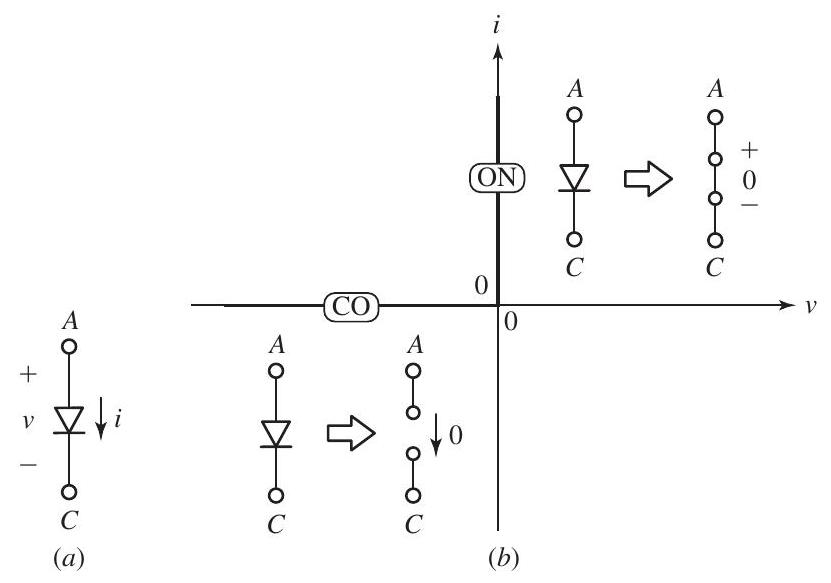
\includegraphics[max width=\textwidth, center]{2024_10_31_0c26dbfd3a789ec9acb1g-018}

FIGURE 1.1 (a) Circuit symbol and sign convention for the diode. (b) Ideal-diode $i$-v characteristic and diode models in the on (ON) region and in the cut-off (CO) region of operation.\\
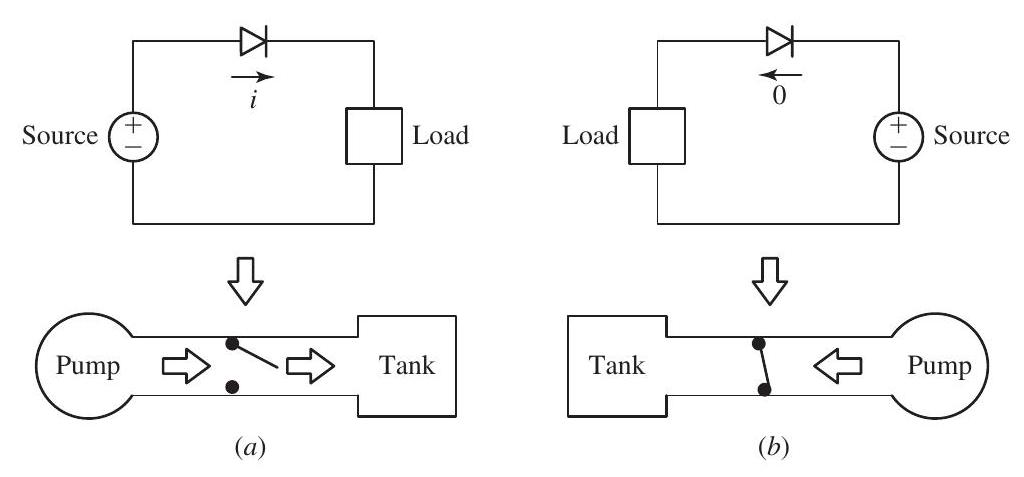
\includegraphics[max width=\textwidth, center]{2024_10_31_0c26dbfd3a789ec9acb1g-019}

FIGURE 1.2 Valve analogy of a diode: (a) forward operation and (b) reverse operation.

When invited to draw current in the direction of its arrowhead ( $i>0$ ), also called the forward ( F ) direction, a diode will eagerly conduct the given current by acting as a short circuit $(v=0)$. In this case the diode is said to be forward biased, or also to be on (ON). However, if we try to force current in the opposite direction, also called the reverse $(\mathrm{R})$ direction, the diode will stubbornly oppose current flow by acting as an open circuit $(i=0)$. The diode is now said to be reverse biased, or also to be cut off $(\mathrm{CO})$. When cut off the diode will sustain whatever voltage $(v<0)$ is imposed by the surrounding circuitry.

Figure $1.1 b$ shows the $i-v$ characteristic of the diode, which we express mathematically as


\begin{align*}
v=0 & \text { for } i>0  \tag{1.1a}\\
i=0 & \text { for } v<0 \tag{1.1b}
\end{align*}


Also shown next to the curves are the diode models (a short circuit and an open circuit) corresponding to the two modes of operation. A device with the characteristic shown is referred to as an ideal diode. As we shall see, practical diodes will only approximate these idealized curves.

A diode can be likened to a water valve according to the analogy of Fig. 1.2. The valve hinges at the top and has a stopper at the bottom. Forcing electric current to a load via a diode is like pumping water to a tank via a pipe equipped with a valve. If pump pressure is applied in the forward direction, the valve will open and allow water to flow as in Fig. 1.2a. However, if pressure is applied in the reverse direction as in Fig. 1.2b, the valve will close and inhibit water flow. To develop a feel for diode operation, let us consider our first circuit example.

EXAMPLE 1.1 (a) In the circuit of Fig. 1.3 let $R_{1}=1 \mathrm{k} \Omega$ and $R_{2}=2 \mathrm{k} \Omega$. If $v_{S}=3 \mathrm{~V}$, find $i_{S}$ so that $D$ draws 1 mA . Show the final circuit.\\
(b) If $i_{S}=3 \mathrm{~mA}$, find $v_{S}$ so that $D$ drops 2 V . Show the circuit.\\
(c) If $i_{S}=2 \mathrm{~mA}$ and $v_{S}=6 \mathrm{~V}$, find $R_{1}$ and $R_{2}$ so that $D$ operates at the origin of the $i-v$ plane, where $v=0$ and $i=0$.\\
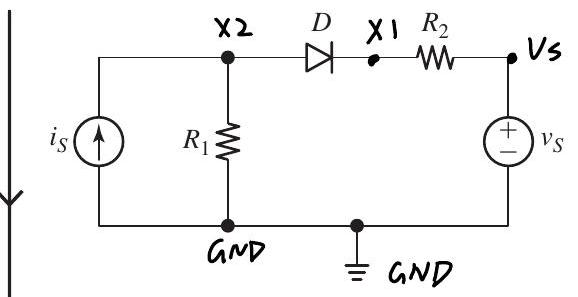
\includegraphics[max width=\textwidth, center]{2024_10_31_0c26dbfd3a789ec9acb1g-020}

FIGURE 1.3 Circuit of Example 1.1.

\section*{Solution}
(a) In conduction $D$ acts as a short-circuit, so $v_{A}=v_{C}$. By Ohm's law and KVL, $v_{A}=v_{C}=(2 \mathrm{k} \Omega) \times(1 \mathrm{~mA})+(3 \mathrm{~V})=5 \mathrm{~V}$, causing the $1-\mathrm{k} \Omega$ resistance to draw $(5 \mathrm{~V}) /(1 \mathrm{k} \Omega)=5 \mathrm{~mA}$, flowing downward. KCL gives $i_{S}=(1 \mathrm{~mA})+$ $(5 \mathrm{~mA})=6 \mathrm{~mA}$, so the situation is as in Fig. 1.4a.\\
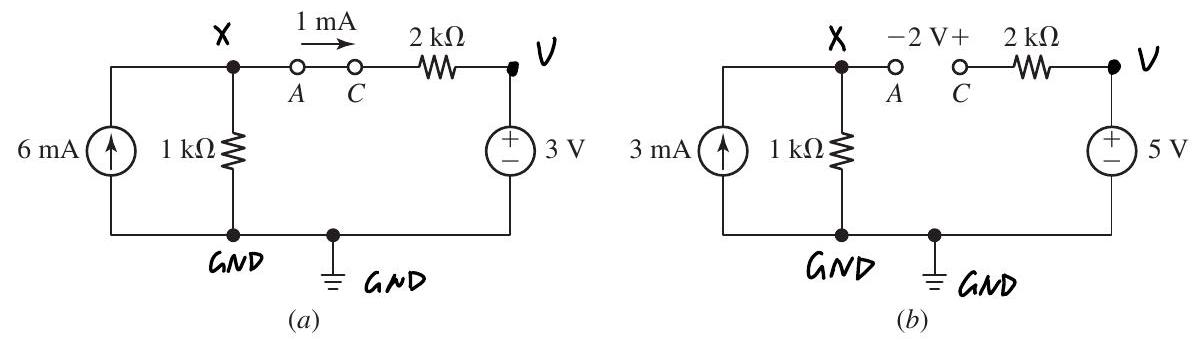
\includegraphics[max width=\textwidth, center]{2024_10_31_0c26dbfd3a789ec9acb1g-020(1)}

FIGURE 1.4 Circuit solutions to Example 1.1.\\
(b) In cutoff $D$ acts as an open circuit, so the $2-\mathrm{k} \Omega$ resistance drops 0 V . By Ohm's law, $v_{A}=3 \times 1=3 \mathrm{~V}$. By KVL, the voltage at the cathode is $v_{C}=v_{A}+2=3+2=5 \mathrm{~V}$, so $v_{S}=v_{C}=5 \mathrm{~V}$ as shown in Fig. 1.4b.\\
(c) $i=0 \Rightarrow v_{C}=v_{S}=6 \mathrm{~V} ; v=0 \Rightarrow v_{A}=v_{C}=6 \mathrm{~V}$ and $R_{1}=v_{A} / i_{S}=6 / 2=$ $3 \mathrm{k} \Omega$. As long as $D$ is cut off, the value of $R_{2}$ is irrelevant. $R_{2}$ has an impact only when $D$ is on.

\section*{Finding the Operating Mode of a Diode}
Even though it consists of two straight segments, the diode characteristic is nonlinear. (In fact, it is said to be piecewise linear.) Yet, as demonstrated by Example 1.1, we can still apply the analytical techniques learned in linear-circuits courses because at any given time the diode operates only in one of its two possible modes (either ON or CO), where it admits a model (open or short circuit) that is indeed linear. Thus, to carry out our analysis, we only need to determine which of the two modes the diode happens to be operating in at a given time.\\
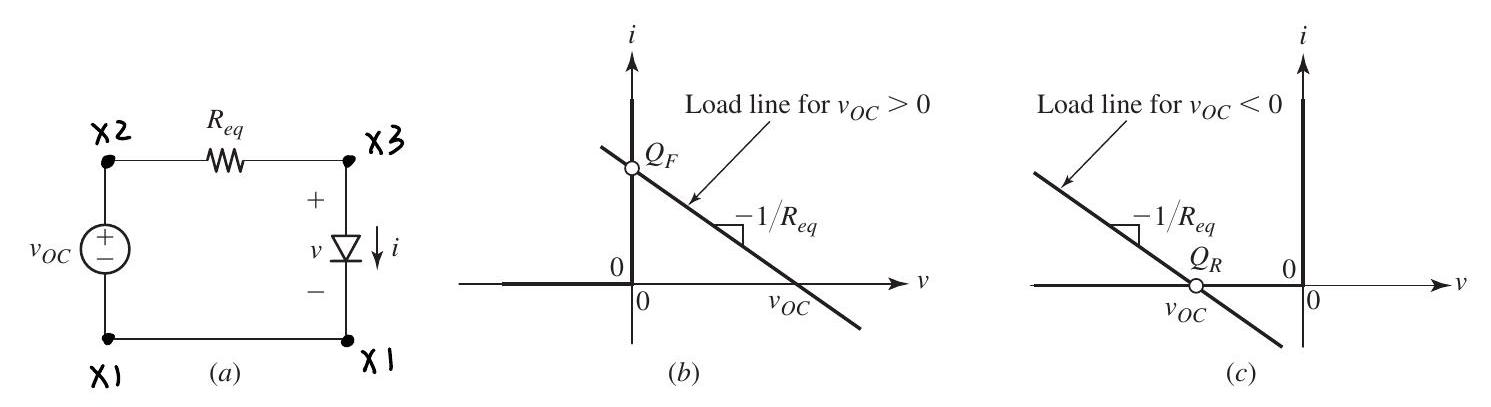
\includegraphics[max width=\textwidth, center]{2024_10_31_0c26dbfd3a789ec9acb1g-021}

There are many situations in which the diode is embedded in a linear circuit, indicating that we can simplify our analysis significantly if we replace the surrounding circuitry with its Thévenin equivalent. After doing so we end up with the basic situation of Fig. 1.5a, where $v_{O C}$ is the open-circuit voltage that the external circuit would sustain between the nodes corresponding to the anode and the cathode, but with the diode removed. (Note that the polarity of $v_{O C}$ is defined positive at the point of connection to the anode!) Moreover, $R_{e q}$ is the external circuit's equivalent resistance as seen by the diode. Shown in Fig. $1.5 b$ and $1.5 c$ is the $i-v$ characteristic of the diode as well as that of the surrounding circuit, the latter being referred to as the load line. As we know from basic circuit theory, the load line is a straight line intercepting the $v$-axis at $v=v_{O C}$, and having a slope of $-1 / R_{e q}$. The circuit's operating point lies at the intersection of the diode curve and the load line, where the diode and the surrounding circuit share the same voltage and current. It is apparent that

\begin{itemize}
  \item If $v_{O C}>0$, the operating point $\left(Q_{F}\right)$ lies on the ON segment, where the diode is forward biased and thus acts as a short circuit to yield
\end{itemize}


\begin{equation*}
v=0 \quad i=\frac{v_{O C}}{R_{e q}}(>0) \tag{1.2a}
\end{equation*}


\begin{itemize}
  \item Conversely, if $v_{O C}<0$, the operating point $\left(Q_{R}\right)$ lies on the CO segment, where the diode is reverse biased and thus acts as an open circuit to yield
\end{itemize}


\begin{equation*}
i=0 \quad v=v_{O C}(<0) \tag{1.2b}
\end{equation*}


Let us illustrate via an actual example.

EXAMPLE 1.2 (a) Find $v$ and $i$ in the circuit of Fig. $1.6 a$ if $v_{S}=12 \mathrm{~V}, R_{1}=10 \mathrm{k} \Omega, R_{2}=30 \mathrm{k} \Omega$, and $R_{3}=R_{4}=15 \mathrm{k} \Omega$.\\
(b) Repeat, but with $R_{2}$ lowered from $30 \mathrm{k} \Omega$ to $2.0 \mathrm{k} \Omega$.\\
(c) What happens if we reverse the diode's direction in part (a)? In part (b)?\\
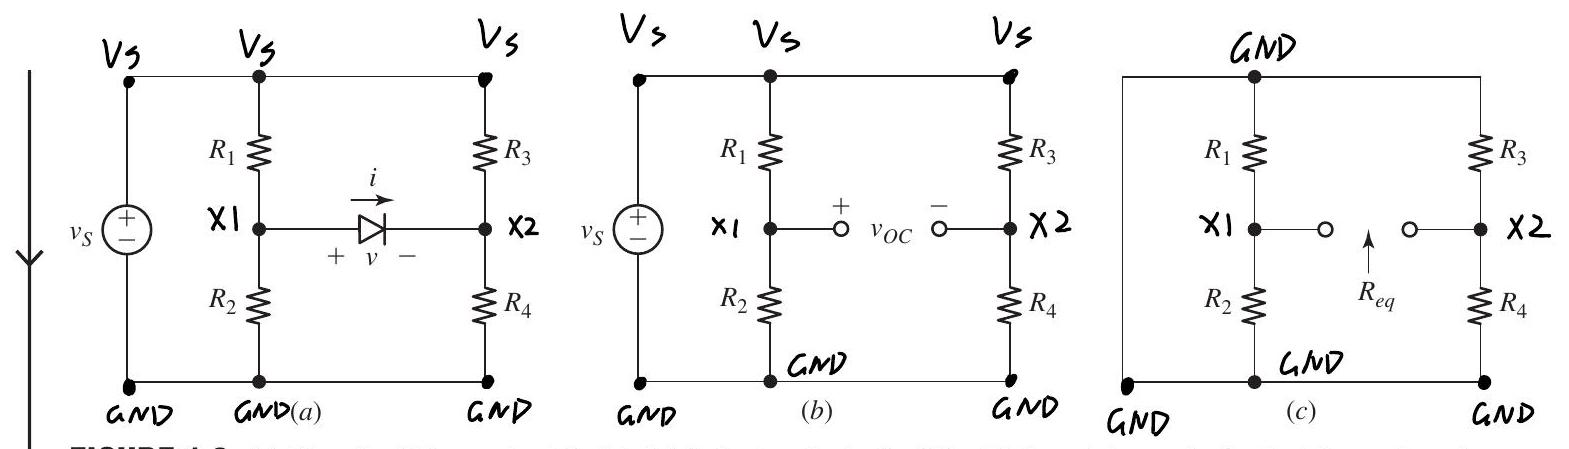
\includegraphics[max width=\textwidth, center]{2024_10_31_0c26dbfd3a789ec9acb1g-022(1)}

FIGURE 1.6 (a) Circuit of Example 1.2. (b), (c) Subcircuits to find the Thévenin's equivalent of the network surrounding the diode. Note that the diode has been removed.

\section*{Solution}
(a) Removing the diode yields the subcircuit of Fig. $1.6 b$, where the voltage divider rule gives

$$
v_{O C}=\left(\frac{R_{2}}{R_{1}+R_{2}}-\frac{R_{4}}{R_{3}+R_{4}}\right) v_{S}
$$

Substituting the given component values gives $v_{O C}=9-6=3 \mathrm{~V}$. Since $v_{O C}>0$, the diode will be on, acting as a short circuit with $v=0$. To find $i$, we need $R_{e q}$. To this end, we suppress the voltage source to obtain the subcircuit of Fig. 1.6c. By inspection,

$$
R_{e q}=\left(R_{1} / / R_{2}\right)+\left(R_{3} / / R_{4}\right)
$$

Substituting the given component values gives $R_{e q}=15 \mathrm{k} \Omega$. Consequently, by Eq. $(1.2 a), i=3 / 15=0.2 \mathrm{~mA}$. The situation is shown in Fig. $1.7 a$, where the student is encouraged to find all other voltages and currents in the circuit as a check.\\
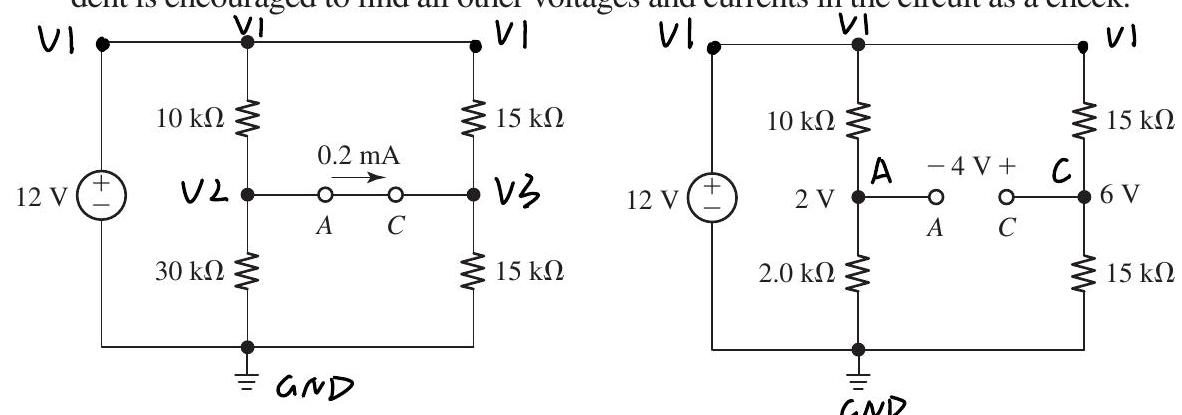
\includegraphics[max width=\textwidth, center]{2024_10_31_0c26dbfd3a789ec9acb1g-022}

FIGURE 1.7 Circuit of Example 1.2a, where the diode is on, and Example 1.1b, where the diode is off.\\
(b) With $R_{2}$ lowered to $2.0 \mathrm{k} \Omega$ we get $v_{O C}=2-6=-4 \mathrm{~V}$. Since we now have $v_{O C}<0$, the diode is off, acting as an open circuit with $i=0$. The situation is depicted in Fig. 1.7b.\\
(c) Reversing the diode direction so that the anode is now at the right and the cathode is at the left will cause the diode to be off in part (a) and on in part ( $b$ ). Thus, in part ( $a$ ) the diode current is zero, and the diode voltage is -3 V . In part (b) we get $R_{e q}=(10 / / 2)+(15 / / 15)=55 / 6 \mathrm{k} \Omega, v=0 \mathrm{~V}$, and $i=4 /(55 / 6)=24 / 55 \mathrm{~mA}$, now flowing toward the left.

\section*{Cut-and-Try Approach}
If the diode is part of a nonlinear circuit, as in the case of multiple-diode circuits, it is generally not possible to perform a Thévenin's reduction of the surrounding circuitry. However, knowing that the diode must be either on or off, we can use intuition to make an educated assumption, and then check that our results are consistent with our assumption, changing the assumption if needed, until we obtain consistent results. A two-diode circuit provides a classic example of the cut-and-try approach.

EXAMPLE 1.3 (a) The circuit of Fig. $1.8 a$ is powered by a dual $\pm 6-\mathrm{V}$ dc power supply system, which we show in concise form (that is, without drawing the actual dc voltage sources) in order to reduce cluttering in the circuit diagram. Find the current $I_{D}$ and voltage $V_{D}$ for each diode.\\
(b) Repeat, but with the resistances interchanged with each other.\\
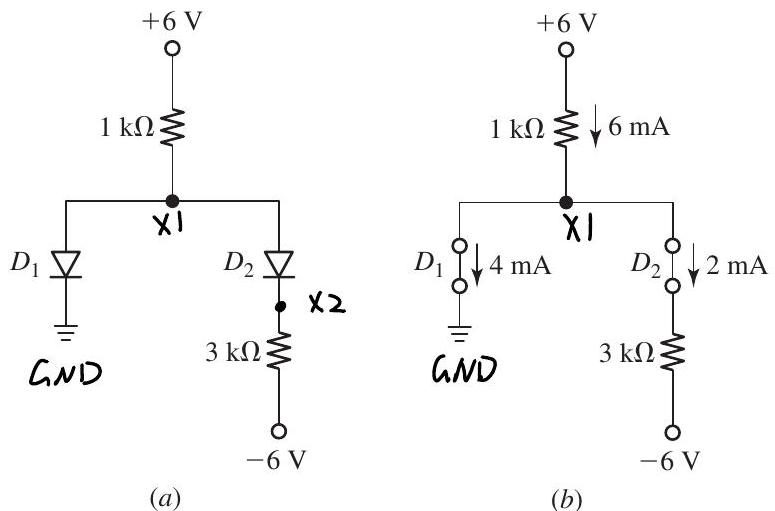
\includegraphics[max width=\textwidth, center]{2024_10_31_0c26dbfd3a789ec9acb1g-023}

FIGURE 1.8 (a) Circuit of Example 13.a. (b) The circuit after it has been solved.

\section*{Solution}
(a) Knowing that each diode has to be either in conduction (ON) or cut off $(\mathrm{CO})$, we have four possibilities: $\left(D_{1}, D_{2}\right)=(\mathrm{CO}, \mathrm{CO}),(\mathrm{CO}, \mathrm{ON}),(\mathrm{ON}, \mathrm{CO})$, (ON, ON). However, considering that the $+6-\mathrm{V}$ source tends to source current to both anodes, and that the $-6-\mathrm{V}$ source tends to sink current from $D_{2}$ 's cathode, it seems reasonable to assume that both diodes be on, or $\left(D_{1}, D_{2}\right)=$ (ON, ON). Thus, replacing each diode with a short circuit, we end up with the situation of Fig. 1.5b, where the diode voltages are

$$
V_{D_{1}}=V_{D_{2}}=0 \mathrm{~V}
$$

Moreover, applying first Ohm's law and then KCL we have

$$
I_{D_{2}}=I_{3 \mathrm{k} \Omega}=\frac{0-(-6)}{3}=2 \mathrm{~mA} \quad I_{D_{1}}=I_{1 \mathrm{k} \Omega}-I_{D_{2}}=\frac{6-0}{1}-2=4 \mathrm{~mA}
$$

Both diodes carry current in the forward direction, so our results are consistent with our initial assumption, and we are done.\\
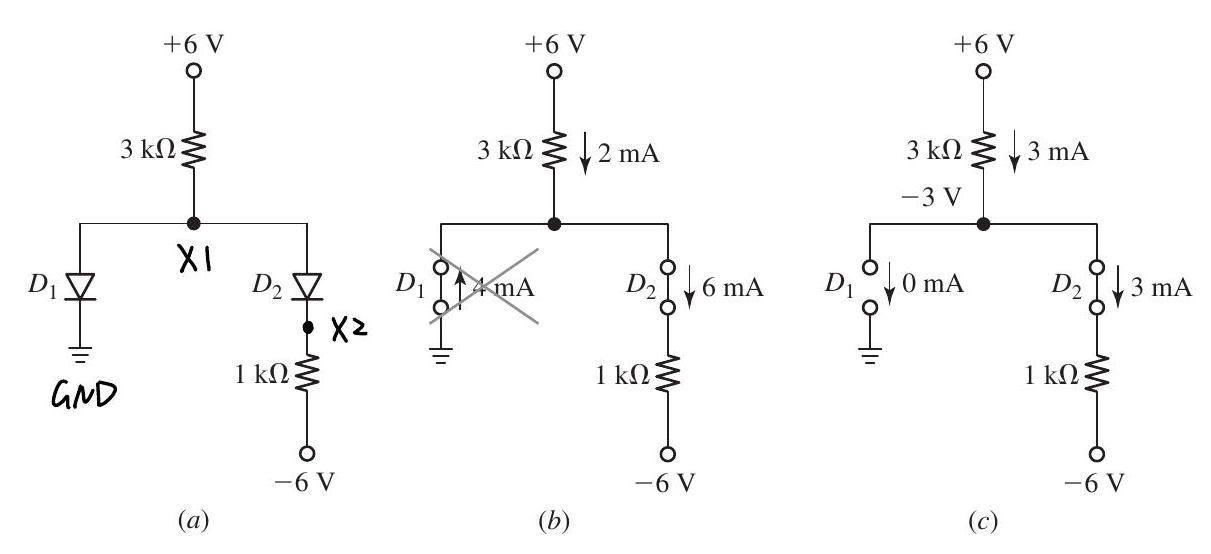
\includegraphics[max width=\textwidth, center]{2024_10_31_0c26dbfd3a789ec9acb1g-024}

FIGURE 1.9 (a) Circuit of Example 1.3b. (b) First attempt (wrong), and (c) second attempt (successful).\\
(b) Swapping the resistances results in the circuit of Fig. 1.9a. We may again assume the state $\left(D_{1}, D_{2}\right)=(\mathrm{ON}, \mathrm{ON})$ and refer to the circuit of Fig. $1.9 b$ for our calculations. By Ohm's law, $I_{3 \mathrm{k} \Omega}=6 / 3=2 \mathrm{~mA}$ and $I_{1 \mathrm{k} \Omega}=[0-(-6)] / 1=6 \mathrm{~mA}$. Then, to satisfy KCL, $D_{1}$ would have to supply 4 mA flowing upward, that is, in the reverse direction. But this is impossible, indicating that the assumption $\left(D_{1}, D_{2}\right)=(\mathrm{ON}, \mathrm{ON})$ was wrong. Yet, we note that $D_{2}$ must be ON because the negative supply draws current from its cathode. The only plausible assumption is thus $\left(D_{1}, D_{2}\right)=(\mathrm{CO}, \mathrm{ON})$, as shown in Fig. 1.9c. We now have

$$
I_{D_{1}}=0 \quad I_{D_{2}}=\frac{6-(-6)}{3+1}=3 \mathrm{~mA}
$$

By KVL, the voltage at the node common to the anodes is $6-(3 \times 3)=-3 \mathrm{~V}$, indicating that $D_{1}$ is indeed reverse biased, as assumed at the onset of our second try. So, $V_{D_{1}}=-3 \mathrm{~V}$, and $V_{D_{2}}=0$.

\section*{Exercise 1.1}
Find $I_{D}$ and $V_{D}$ for each diode in the circuit of Fig. $1.9 a$ if (a) the direction of $D_{1}$ is reversed while $D_{2}$ is as shown; (b) the direction of $D_{2}$ is reversed while $D_{1}$ is as shown; $(c)$ the direction of each diode in Fig. 1.9a is reversed.\\
Ans. (a) $I_{D_{1}}=4 \mathrm{~mA}, V_{D_{1}}=0, I_{D_{2}}=6 \mathrm{~mA}, V_{D_{2}}=0$; (b) $I_{D_{1}}=2 \mathrm{~mA}, V_{D_{1}}=0$, $I_{D_{2}}=0, V_{D_{2}}=-6 \mathrm{~V}$; (c) $I_{D_{1}}=I_{D_{2}}=0, V_{D_{1}}=-6 \mathrm{~V}, V_{D_{2}}=-12 \mathrm{~V}$.

\section*{Concluding Observations}
Even though the diode is the simplest electronic element, it offers a glimpse into important features that are common to other more complex electronic devices, such as transistors to be studied later.

\begin{itemize}
  \item The diode is a classic example of a nonlinear circuit element.
  \item Strictly speaking, the analysis techniques learned in linear-circuits courses cannot be applied to nonlinear elements. However, every attempt should be made to\\
approximate the $i-v$ characteristics with piecewise linear segments, for then we can create separate linear models for the device, one for each region of operation.
  \item Once we know which region the device finds itself operating in at a given moment, we can apply familiar linear-analysis techniques to investigate its behavior over that particular region.
\end{itemize}

Quite often a cut-and-try approach may be required in order to determine the actual region of operation. This approach involves the following steps:

\begin{itemize}
  \item Start out by making an educated assumption about the region of operation of each nonlinear device.
  \item Replace each device with the linear model pertaining to that region, and proceed with a linear analysis of the resulting circuit.
  \item Check that the results are consistent with your initial assumption. If they are, we are finished. If they aren't, we need to change our initial assumption until consistent results are obtained.
\end{itemize}

We shall encounter plenty of examples as we proceed. Lastly, it must be said that computer simulation, such as PSpice, is a powerful tool not only to corroborate any assumptions that we make, but also to provide refinements and details that a piecewise linear approximation of necessity often misses.

\subsection*{1.2 BASIC DIODE APPLICATIONS}
Having introduced the fundamentals of diode behavior and diode circuit analysis, we are now ready to examine some of the most common diode applications.

\section*{Rectifiers}
Figure $1.10 a$ depicts one of the most popular diode applications, namely, signal rectification. During the positive alternations of $v_{I}$ the diode is on and the circuit gives $v_{O}=v_{I}$ (see Fig. 1.10b). During the negative alternations of $v_{I}$ the diode is cut off, and the circuit gives $v_{O}=0 \mathrm{~V}$ (see Fig. 1.10c). Figure 1.11a shows the response $v_{O}$ to a sinusoidal input $v_{I}$. We say that the circuit passes on to the load $R$ only the positive portions of the input waveform, while the negative portions are inhibited. We observe that while $v_{I}$ alternates in polarity and averages out to zero, $v_{O}$ is unipolar and thus exhibits a nonzero average, or a nonzero dc component. For this reason the circuit is referred to as rectifier. Its behavior can be visualized also via the voltage\\
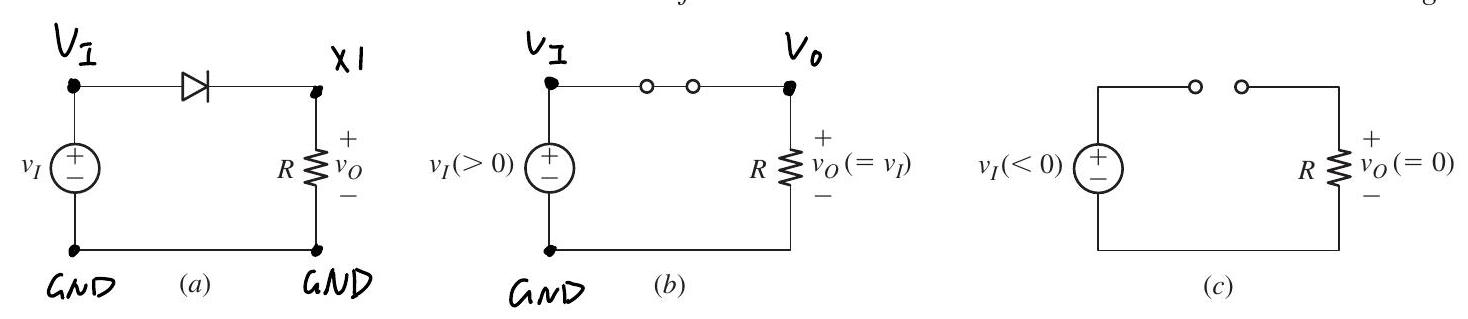
\includegraphics[max width=\textwidth, center]{2024_10_31_0c26dbfd3a789ec9acb1g-025}

FIGURE 1.10 (a) Half-wave rectifier and its equivalent circuits for (b) $v_{l}>0$ and (c) $v_{l}<0$.\\
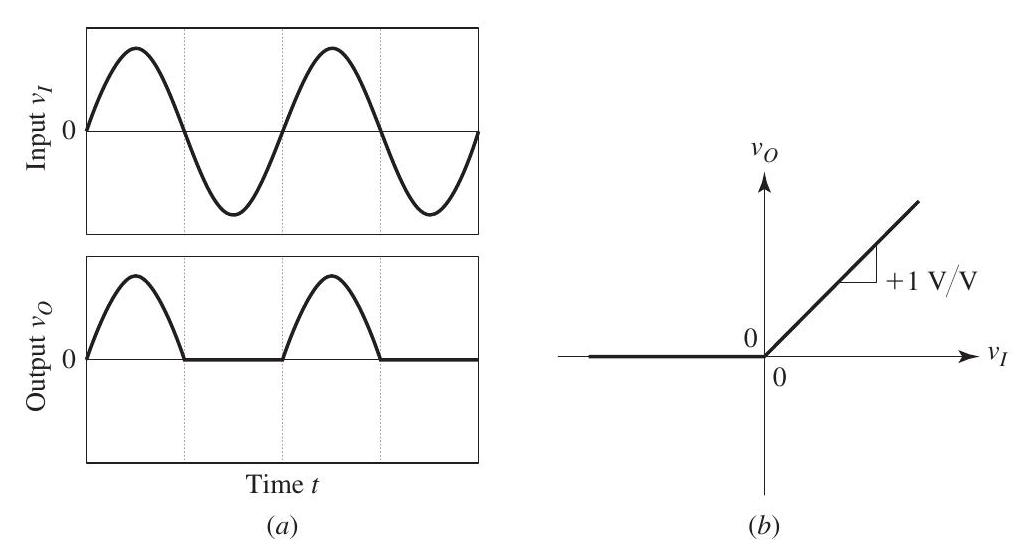
\includegraphics[max width=\textwidth, center]{2024_10_31_0c26dbfd3a789ec9acb1g-026(3)}

FIGURE 1.11 Illustrating half-wave rectification via (a) the input/output waveforms and ( $b$ ) the VTC.\\
transfer curve (VTC), representing the plot of $v_{O}$ versus $v_{I}$. This curve, expressed mathematically as

\[
\begin{array}{ll}
v_{O}=v_{I} & \text { for } v_{I}>0 \\
v_{O}=0 & \text { for } v_{I}<0 \tag{1.3b}
\end{array}
\]

is shown in Fig. 1.11b. Needless to say, the presence of the diode results in a nonlinear VTC. The student can easily verify that reversing the diode interconnection in Fig. 1.10a results in a rectifier that passes only the negative portions of the input waveform.

Since it passes only half the input wave, the circuit of Fig. 1.10a is called a halfwave rectifier. By contrast, a full-wave rectifier passes both halves of the input wave, one unchanged and the other inverted. Also called absolute-value circuit, it is implemented using the four-diode arrangement of Fig. 1.12a, known as a diode bridge. To understand its operation, consider first the case $v_{I}>0$, then the case $v_{I}<0$.

\begin{itemize}
  \item For $v_{I}>0$ we expect the input source $v_{I}$ to source current to $D_{1}$ 's anode and to sink current from $D_{4}$ 's cathode, causing both diodes to be on, as depicted in Fig. 1.12b. Under these circumstances we have $v_{O}=v_{I}(>0)$. Moreover, we note that both $D_{2}$ and $D_{3}$ are reverse biased by the amount $v_{0}$, as also shown in Fig. 1.12b. The current loop is thus source $\rightarrow D_{1} \rightarrow R \rightarrow D_{4} \rightarrow$ source.\\
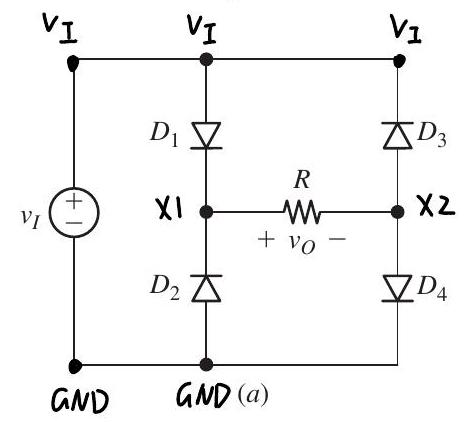
\includegraphics[max width=\textwidth, center]{2024_10_31_0c26dbfd3a789ec9acb1g-026(1)}\\
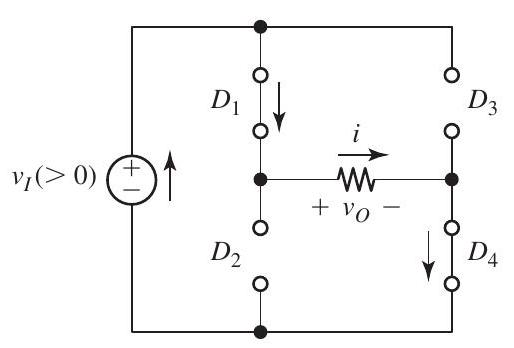
\includegraphics[max width=\textwidth, center]{2024_10_31_0c26dbfd3a789ec9acb1g-026(2)}\\
(b)\\
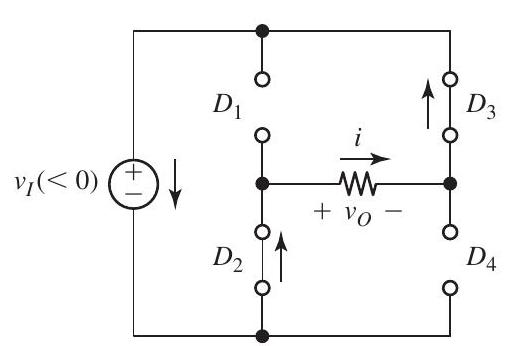
\includegraphics[max width=\textwidth, center]{2024_10_31_0c26dbfd3a789ec9acb1g-026}\\
(c)
\end{itemize}

FIGURE 1.12 (a) Full-wave rectifier and its equivalent circuits for (b) $v_{l}>0$ and (c) $v_{l}<0$.\\
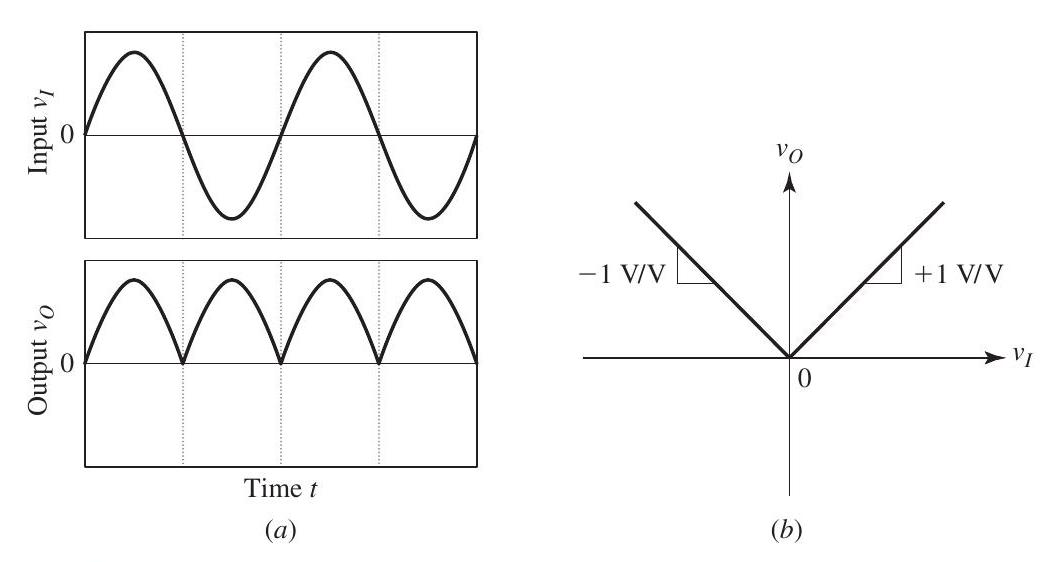
\includegraphics[max width=\textwidth, center]{2024_10_31_0c26dbfd3a789ec9acb1g-027}

FIGURE 1.13 Illustrating full-wave rectification via (a) the input/output waveforms and (b) the VTC.

\begin{itemize}
  \item For $v_{I}<0$ we expect the input source $v_{I}$ to sink current from $D_{3}$ 's cathode and to source current to $D_{2}$ 's anode, causing both diodes to be on, as depicted in Fig. 1.12c. We now have $v_{O}=-v_{I}$, or $v_{O}>0$ because $v_{I}<0$. Moreover, both $D_{1}$ and $D_{4}$ are now reverse biased, as also shown in Fig. 1.12c. The current loop is now source $\rightarrow$ $D_{2} \rightarrow R \rightarrow D_{3} \rightarrow$ source. We observe that the current through $R$ flows toward the right in both cases, confirming the absolute-value function mentioned earlier.\\
Figure $1.13 a$ shows the response $v_{O}$ to a sinusoidal input $v_{I}$, while Fig. $1.13 b$ shows the VTC, which we express concisely as
\end{itemize}


\begin{equation*}
v_{O}=\left|v_{I}\right| \tag{1.4}
\end{equation*}


Rectifier circuits find application in power electronics, communications, and instrumentation.

EXAMPLE 1.4 (a) Shown in Fig. 1.14 is a simple-if not overly efficient—circuit for charging a $12-\mathrm{V}$ car battery. Assuming $v_{S}$ is an ac source with a $24-\mathrm{V}$ peak amplitude obtained from the household ac power via a step-down transformer, sketch and label $v_{S}$ as well as the battery current $i$.\\
(b) Find the fraction of each ac cycle during which the battery receives current.

\section*{Solution}
(a) It is apparent that as long as $\left|v_{S}\right| \leq 12 \mathrm{~V}$, all diodes are cut off and $i=0$. However, as soon as $v_{S}$ rises above $12 \mathrm{~V}, D_{1}$ and $D_{4}$ go on, thus establishing the current loop

$$
\text { source } \rightarrow R \rightarrow D_{1} \rightarrow \text { battery } \rightarrow D_{4} \rightarrow \text { source }
$$

Conversely, when $v_{S}$ drops below $-12 \mathrm{~V}, D_{2}$ and $D_{3}$ go on, thus establishing the current loop

$$
\text { source } \rightarrow D_{2} \rightarrow \text { battery } \rightarrow D_{3} \rightarrow R \rightarrow \text { source }
$$

\begin{center}
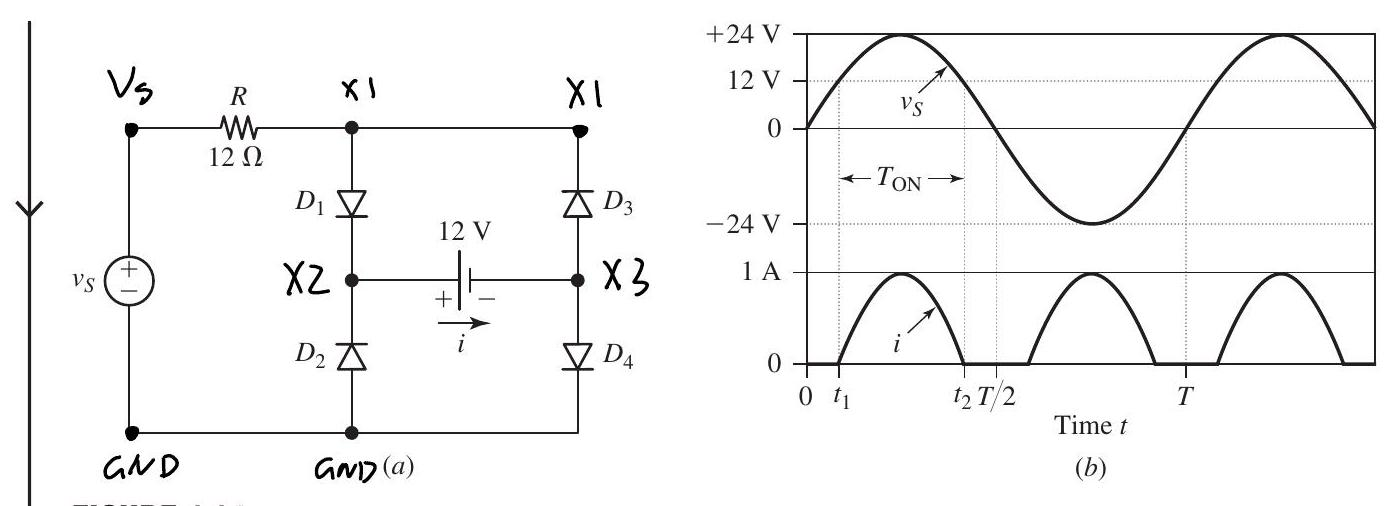
\includegraphics[max width=\textwidth]{2024_10_31_0c26dbfd3a789ec9acb1g-028(1)}
\end{center}

FIGURE 1.14 (a) Simple battery charger, and (b) voltage and current waveforms.\\
In either case, we have

$$
i=0 \quad \text { for } \quad\left|v_{S}\right| \leq 12 \mathrm{~V} \quad i=\frac{v_{S}-12 \mathrm{~V}}{R} \quad \text { for } \quad\left|v_{S}\right|>12 \mathrm{~V}
$$

The peak value of the current is $(24-12) / 12=1 \mathrm{~A}$. The waveforms are shown in Fig. 1.14b.\\
(b) During the first cycle, $i$ starts to flow into the battery at the instant $t_{1}$ such that

$$
24 \sin \frac{2 \pi t_{1}}{T}=12
$$

or $t_{1}=T / 12$, and stops conducting at $t_{2}=T / 2-T / 12$. Consequently, the conduction interval is $T_{\mathrm{ON}}=t_{2}-t_{1}=T / 3$, or $T_{\mathrm{ON}}=(2 / 3)(T / 2)$, where $T / 2$ is the period of the current waveform. In summary, the battery receives current during $2 / 3$ of the time.

\section*{Diode Logic Gates}
Figures $1.15 a$ and $1.16 a$ show how diodes can be used to implement elementary functions of the logic type, which are at the basis of digital systems. The inputs $A$ and $B$ and the output $Y$ are binary-valued voltages that can be either low $(L)$, such as 0 V , or high $(H)$, such as the power-supply voltage $V_{S}$ (typically, 5 V$)$. Circuit behavior is best understood by examining the rows of the accompanying tables, one at a time.\\
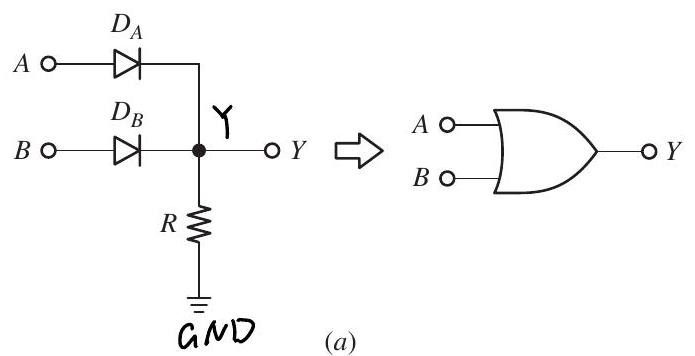
\includegraphics[max width=\textwidth, center]{2024_10_31_0c26dbfd3a789ec9acb1g-028}

\begin{center}
\begin{tabular}{|c|c|c|c|c|}
\hline
$A$ & $B$ & $D_{A}$ & $D_{B}$ & $Y$ \\
\hline
$L$ & $L$ & CO & CO & $L$ \\
\hline
$L$ & $H$ & CO & ON & $H$ \\
\hline
$H$ & $L$ & ON & CO & $H$ \\
\hline
$H$ & $H$ & ON & ON & $H$ \\
\hline
\end{tabular}
\end{center}

(b)

FIGURE 1.15 (a) Diode circuit implementing the OR function, and (b) its truth table.\\
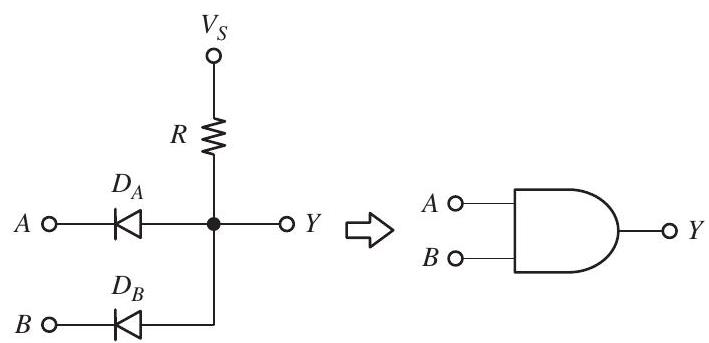
\includegraphics[max width=\textwidth, center]{2024_10_31_0c26dbfd3a789ec9acb1g-029}\\
(a)

\begin{center}
\begin{tabular}{|c|c|c|c|c|}
\hline
$A$ & $B$ & $D_{A}$ & $D_{B}$ & $Y$ \\
\hline
$L$ & $L$ & ON & ON & $L$ \\
\hline
$L$ & $H$ & ON & CO & $L$ \\
\hline
$H$ & $L$ & CO & ON & $L$ \\
\hline
$H$ & $H$ & CO & CO & $H$ \\
\hline
\end{tabular}
\end{center}

(b)

FIGURE 1.16 (a) Diode circuit implementing the AND function, and (b) its truth table.

\begin{itemize}
  \item As long as both inputs $A$ and $B$ are low $(0 \mathrm{~V})$ in Fig. $1.15 a$, both diodes are off, so all voltages and currents are zero, and $Y$ is low. However, if we drive at least one input high ( 5 V ), we will be sourcing current to the anode of the corresponding diode, turning it on and thus pulling $Y$ also high, as illustrated in Fig. 1.15b. We summarize by saying that $Y$ is high if $A$ or $B$ or both are high. This logic function, aptly called the OR function, is identified by the logic-gate symbol next to the circuit itself, in Fig. 1.15a. The table of Fig. $1.15 b$ summarizes its behavior and is called the truth table.
  \item As long as at least one input is low $(0 \mathrm{~V})$ in Fig. 1.16a, the corresponding diode will be on as we are sinking current from its cathode. So, $Y$ is also low. Only if both $A$ and $B$ are high will both diodes be cut off, causing the current through $R$ to drop to zero. With zero current, the voltage drop across $R$ is also zero, and we say that $R$ pulls $Y$ to $V_{S}$, or high, as illustrated in Fig. 1.16b. This state of affairs is summarized by saying that $Y$ is high if $A$ and $B$ are high. This logic function, aptly called the AND function, is identified by the logic-gate symbol next to the circuit itself, in Fig. 1.16 $a$. The table of Fig. $1.16 b$ summarizes its behavior and is called the truth table.
\end{itemize}

Each gate can readily be expanded to handle more than just two inputs by interconnecting additional diodes, as needed. The above gates, though certainly useful, are not sufficient to build a complete digital system because we also need, among others, the inversion function. This requires a transistor, as we shall study in the next two chapters.

\section*{Voltage Clamps}
The unidirectional-switch behavior of the diode can be exploited to establish prescribed limits for certain voltages in a circuit. Such a situation arises, for instance, in connection with the inputs to integrated circuits (ICs), which must be kept within limits as recommended in the data sheets in order to prevent the IC from malfunctioning or, even worse, from undergoing permanent damage. As a rule, the input voltages to an IC should never be allowed to exceed its power-supply voltages.

Figure 1.17 a illustrates the situation for a single-supply IC, such as a CMOS digital circuit or a single-supply op amp. However, the principle can readily be generalized to multiple-supply systems, such as dual-supply op amps. With reference to Fig. $1.17 a$, we readily see that as long as the external input $v_{I}$ lies within the range $0 \leq v_{I} \leq V_{S}$, both diodes are off, so the signal right at the IC's input pin is $v_{I C} \cong v_{I}$\\
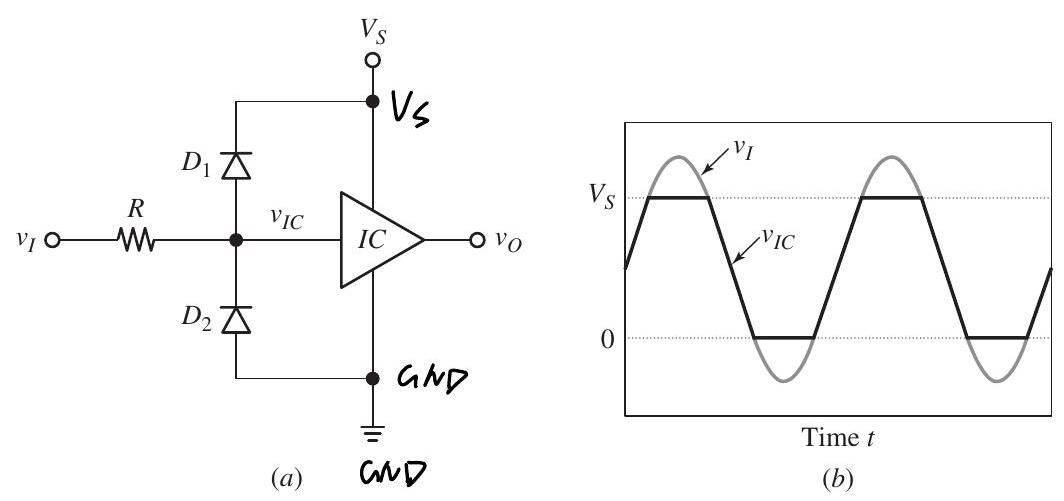
\includegraphics[max width=\textwidth, center]{2024_10_31_0c26dbfd3a789ec9acb1g-030}

FIGURE 1.17 (a) Using diode clamps to limit the input voltage range of an IC.\\
(b) Waveforms.\\
(assuming the IC draws negligible input current, which is indeed the case with CMOS logic circuits as well as op amps.) However, should $v_{I}$ exceed the supply voltage $V_{S}$, either because of an oversight by the user or because of interference noise superimposed upon $v_{I}$ itself, $D_{1}$ will go on, thus establishing a short between $v_{I C}$ and $V_{S}$. We say that $D_{1}$ clamps $v_{I C}$ at $V_{S}$. By similar reasoning, should $v_{I}$ drop below ground potential, $D_{2}$ will clamp $v_{I C}$ at 0 V . As depicted in Fig. $1.17 b$, the diodes protect the IC against possible input overdrive situations by limiting the input-pin voltage within the range

$$
0 \leq v_{I C} \leq V_{S}
$$

For this reason, a diode clamp is also referred to as a limiter, and since it clips the portions of the input waveform falling outside the allowed range, it is also called a clipper.

The need for protection against input overdrives is so important and so common that many ICs come already equipped with internal diode-clamping networks to relieve the user from this worry. In this respect it is worth mentioning the MOSFET as a device particularly sensitive to input overvoltages when handled by humans. Since its gate terminal is the plate of an extremely tiny capacitor, any electrostatic charge that may have accumulated on the body of the user will be transferred to this capacitor during manual contact, thus leading to potentially high voltages (as per $V=Q / C$ ) that are likely to destroy the capacitor's dielectric. However, in the presence of suitable diode clamps, the body of the handler will discharge through one of the diodes, saving the device from assured destruction.

\section*{Exercise 1.2}
In the circuit of Fig. 1.17 let $R=10 \mathrm{k} \Omega$ and $V_{S}=5 \mathrm{~V}$. Assuming the IC draws no current at its input terminal, find the current through $R$ (magnitude and direction) for the following values of $v_{I}:(a)=1 \mathrm{~V},(b) 8 \mathrm{~V},(c)-2 \mathrm{~V},(d) 4.5 \mathrm{~V}$. (e) If it is found that $R$ draws 0.25 mA flowing toward the right, what do you conclude about $v_{I}$ ? ( $f$ ) What if $R$ draws 0.5 mA flowing toward the left? $(g)$ What if the current through $R$ is zero?\\
Ans. (a) 0 mA ; (b) $0.3 \mathrm{~mA}(\rightarrow)$; (c) $0.2 \mathrm{~mA}(\leftarrow)$; (d) 0 mA ; (e) $v_{I}=7.5 \mathrm{~V}$; (f) $v_{I}=-5 \mathrm{~V}$; (g) $0 \leq v_{I} \leq 5 \mathrm{~V}$.

\section*{Piecewise-Linear Function Generators}
The nonlinear characteristic of the diode can be exploited on purpose to create piecewise-linear approximations to nonlinear functions. A popular application example is the conversion of a triangular wave to a sinewave. Figure $1.18 a$ shows a simple example of a piecewise-linear function generator. We make the following observations:\\
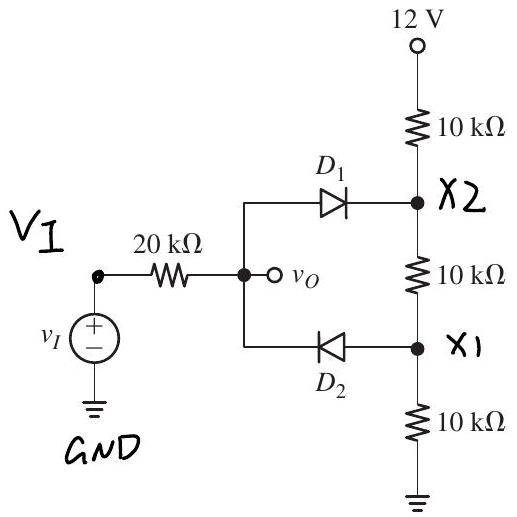
\includegraphics[max width=\textwidth, center]{2024_10_31_0c26dbfd3a789ec9acb1g-031(1)}\\
(a) GND\\
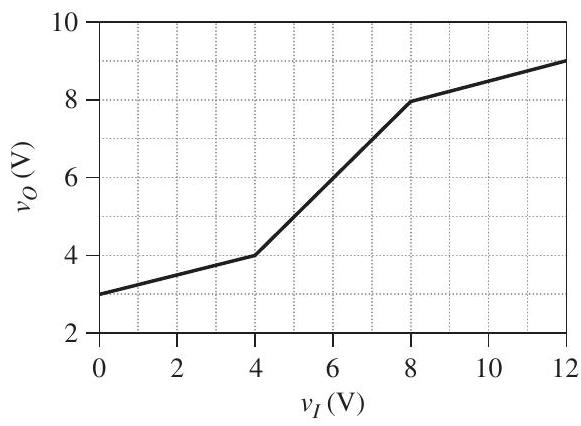
\includegraphics[max width=\textwidth, center]{2024_10_31_0c26dbfd3a789ec9acb1g-031}\\
(b)

FIGURE 1.18 (a) Piecewise-linear function generator example, and (b) its VTC.

\begin{itemize}
  \item With both diodes off, the three $10-\mathrm{kV}$ resistors partition the $12-\mathrm{V}$ supply voltage into three equal voltage drops, thus giving 4 V and 8 V , respectively. This is illustrated in Fig. 1.19a, where we observe that both diodes are off as long as the input is kept within the range $4 \mathrm{~V}<v_{I}<8 \mathrm{~V}$. Since no current flows through the $20-\mathrm{k} \Omega$ resistor, the latter drops 0 V , so the circuit gives
\end{itemize}


\begin{equation*}
v_{O}=v_{I} \quad \text { for } 4 \mathrm{~V}<v_{I}<8 \mathrm{~V} \tag{1.5a}
\end{equation*}


\begin{center}
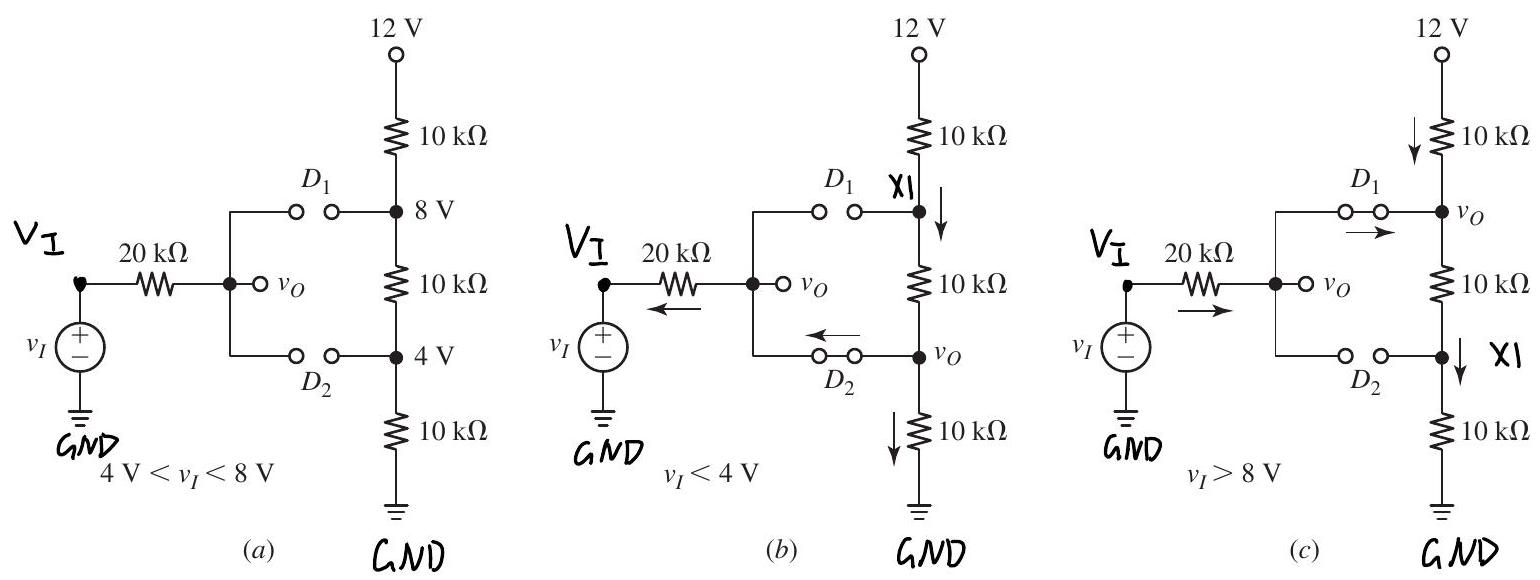
\includegraphics[max width=\textwidth]{2024_10_31_0c26dbfd3a789ec9acb1g-031(2)}
\end{center}

FIGURE 1.19 Equivalent circuits of the function generator of Fig. 1.18 for different input conditions.\\
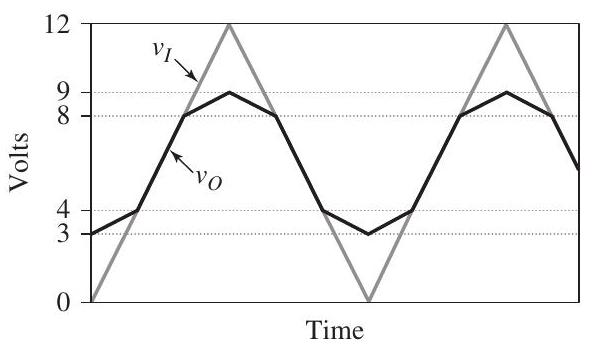
\includegraphics[max width=\textwidth, center]{2024_10_31_0c26dbfd3a789ec9acb1g-032}

FIGURE 1.20 Illustrating the waveshaping effect of the piecewise-linear circuit of Fig. 1.18a.

\begin{itemize}
  \item If we lower $v_{I}$ below $4 \mathrm{~V}, D_{2}$ goes on while $D_{1}$ remains off, resulting in the situation of Fig. 1.19b. By KCL we have
\end{itemize}

$$
\frac{12-v_{O}}{10+10}=\frac{v_{O}-v_{I}}{20}+\frac{v_{O}}{10}
$$

which is readily solved for $v_{O}$ to give


\begin{equation*}
v_{O}=0.25 v_{I}+3 \mathrm{~V} \quad \text { for } v_{I}<4 \mathrm{~V} \tag{1.5b}
\end{equation*}


\begin{itemize}
  \item If we raise $v_{I}$ above $8 \mathrm{~V}, D_{1}$ goes on while $D_{2}$ remains off, resulting in the situation of Fig. 1.19c. Applying again KCL, we get
\end{itemize}

$$
\frac{v_{I}-v_{O}}{20}+\frac{12-v_{O}}{10}=\frac{v_{O}}{10+10}
$$

which is readily solved for $v_{O}$ to give


\begin{equation*}
v_{O}=0.25 v_{I}+6 \mathrm{~V} \quad \text { for } v_{I}>8 \mathrm{~V} \tag{1.5c}
\end{equation*}


Figure $1.18 b$ shows the circuit's VTC. Clearly, we have three separate regions of operation. Within each region, the VTC is a straight segment whose analytical expression is obtained by drawing the corresponding equivalent circuit, as per Fig. 1.19, and subjecting it to elementary linear analysis techniques. This is typical of diode circuits.

Figure 1.20 shows the waveshaping effect of the circuit of Fig. 1.18 upon a triangular wave. Here, the aim is to compress the top and the bottom of the triangle to approximate a sine. Clearly, the present example provides a rather crude approximation, but it is not hard to imagine that we can improve it by using additional segments. This is normally accomplished with $p n$ junction diodes. As we shall see, the characteristic of the $p n$ diode has a rounded knee which helps ensure a smoother transition from one segment to the next of the VTC.

\section*{Peak Detectors}
Additional interesting applications arise if a diode $D$ is partnered by a capacitor $C$. As our first example we consider the circuit of Fig. 1.21a, known as a peak detector. To understand its operation, refer to the waveforms of Fig. 1.21b, where $C$ is assumed initially discharged. As $v_{I}$ swings positive, current will be sourced to the anode, forcing $D$ to conduct and thus to charge up $C$. Since $D$ acts as a short circuit, $v_{O}$ simply follows $v_{I}$.\\
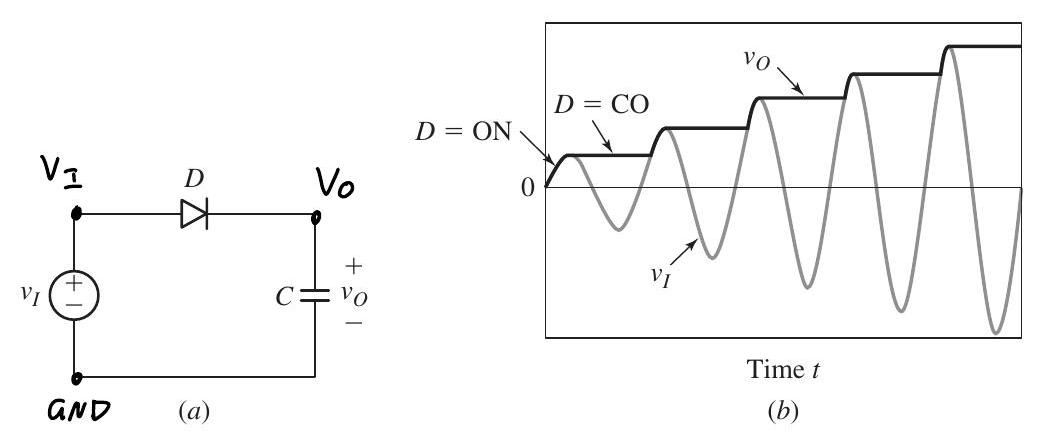
\includegraphics[max width=\textwidth, center]{2024_10_31_0c26dbfd3a789ec9acb1g-033(1)}

FIGURE 1.21 (a) Peak detector, and (b) illustrative waveforms.\\
Once $v_{I}$ peaks out, the anode will start swinging negative relative to the cathode, turning $D$ off and thus leaving $C$ to hold the previously acquired voltage, whose value coincides with that of the previous input peak. This memory action by $C$ will persist until $v_{I}$ rises again to a new, higher peak. When this happens, $D$ will go on again, charging up $C$ to this new peak.

It is apparent that the diode's directionality causes the capacitor voltage to experience only increases, this being the reason why the circuit shown is said to be a positive peak detector. Reversing the diode interconnection in the circuit will cause the capacitor voltage to experience only decreases, thus yielding a negative peak detector. Peak detectors are at the basis of demodulators in the detection of audio signals in amplitude-modulation (AM) radio receivers.

\section*{The Clamped Capacitor or Dc Restorer}
In the circuit of Fig. $1.22 a$ the diode provides a clamping function that prevents $v_{O}$ from ever going negative. To understand circuit operation, refer to the waveforms of Fig. $1.22 b$, where the input is a sine wave alternating between $+V_{m}$ and $-V_{m}$, and $C$ is assumed initially discharged. During the initial positive alternation of $v_{I}$ we simply have $v_{O}=v_{I}$ as the voltage across $C$ is zero and the diode is off. However, as $v_{I}$ goes below 0 V for the first time, the input source will sink current from $D$ 's cathode via $C$, thus turning $D$ on and forcing $C$ to charge. As $v_{I}$ reaches its negative peak of $-V_{m}$ at $t=t_{2}$,\\
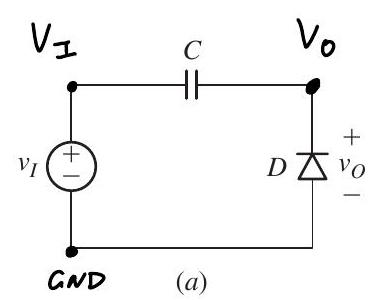
\includegraphics[max width=\textwidth, center]{2024_10_31_0c26dbfd3a789ec9acb1g-033}\\
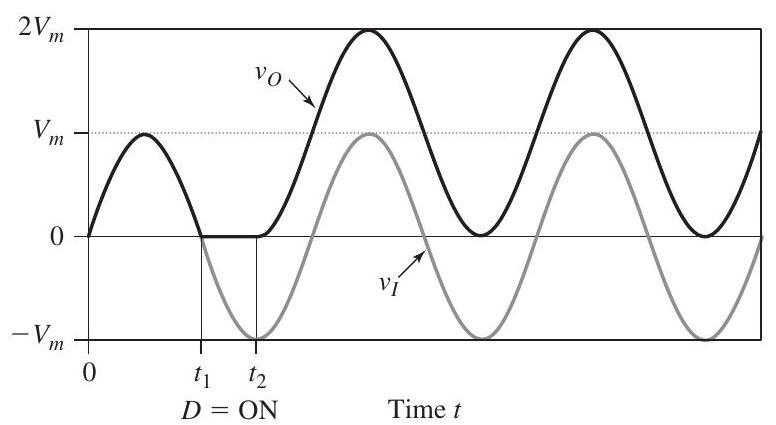
\includegraphics[max width=\textwidth, center]{2024_10_31_0c26dbfd3a789ec9acb1g-033(2)}\\
(b)

FIGURE 1.22 (a) Clamped capacitor, and (b) illustrative waveforms.\\
$C$ will have acquired a voltage equal to $V_{m}$, positive at the right plate. After $t=t_{2}$, the diode will never conduct again, and $C$ will retain the voltage acquired last, thus giving


\begin{equation*}
v_{O}=v_{I}+V_{m} \tag{1.6}
\end{equation*}


for $t \geq t_{2}$. While $v_{I}$ alternates between $-V_{m}$ and $+V_{m}$, and thus averages out to zero, $v_{O}$ ends up alternating between 0 and $+2 V_{m}$ because of the voltage offset provided by $C$. Consequently, $v_{O}$ averages out to $+V_{m}$, and because of this nonzero dc component at its output, the circuit is also referred to as a dc restorer.

\section*{Voltage Multipliers and PSpice Simulation}
An interesting property of the clamped-capacitor circuit of Fig. $1.22 a$ is that it provides a positive output peak that is twice that of the input. This indicates that if we feed the output of the clamped capacitor circuit to a peak detector, we can synthesize a dc voltage of value $+2 V_{m}$, that is, of twice the amplitude of the input! To better understand the behavior of this composite circuit, we simulate it via PSpice. Aptly called a voltage doubler, the circuit is shown in Fig. 1.23 for the case of a 1-kHz, 10-V sinusoidal input. The circuit utilizes pseudo-ideal diodes, whose PSpice models have been created by editing one of the already existing diode models available in PSpice's library, and then setting the parameters $I_{s}$ and $n$ to the values shown in the table (more on this in Appendix 1A).

The various waveforms are displayed in Fig. 1.24, where we observe that after a transient situation lasting less than ten cycles, the output settles to the dc value


\begin{equation*}
v_{2} \rightarrow 2 V_{m} \tag{1.7}
\end{equation*}


or $v_{2}=20 \mathrm{~V}$ in the present example. The reason it takes several cycles to attain the desired steady-state situation is that $C_{1}$ is being loaded by $C_{2}$. If the circuit were implemented with $C_{1} \gg C_{2}$, steady state would be achieved essentially at the second positive peak of $v_{I}$. However, with equal capacitors, which is how the circuit is usually implemented, the charge accumulated by $C_{1}$ at each positive peak of $v_{I}$ redistributes equally between $C_{1}$ and $C_{2}$, causing a reduction in $v_{1}$ which, though significant at the first peak of $v_{l}$, becomes progressively less relevant with each subsequent peak. One can prove (see Exercise 1.3), that the values attained by $v_{2}$ at each peak of $v_{I}$ are $5 \mathrm{~V}, 12.5 \mathrm{~V}, 16.25 \mathrm{~V}, 18.125 \mathrm{~V}$. . . .\\
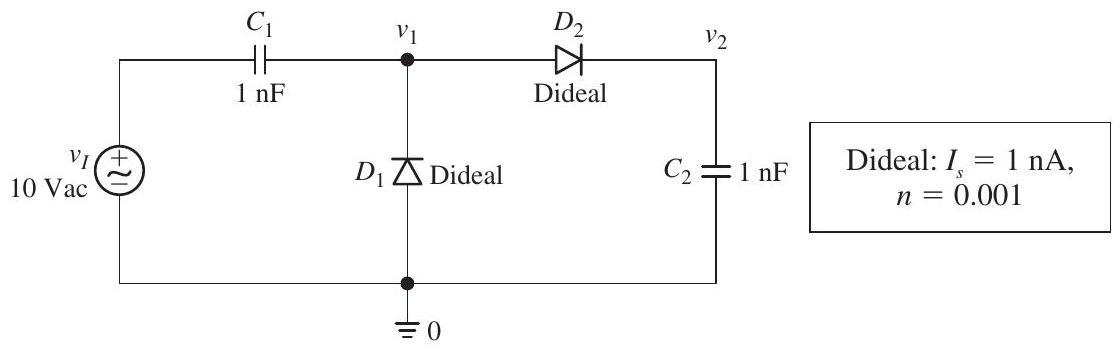
\includegraphics[max width=\textwidth, center]{2024_10_31_0c26dbfd3a789ec9acb1g-034}

FIGURE 1.23 PSpice circuit simulating a voltage doubler based on pseudo-ideal diodes. The parameters of the PSpice diode model are shown inside the box at the right.\\
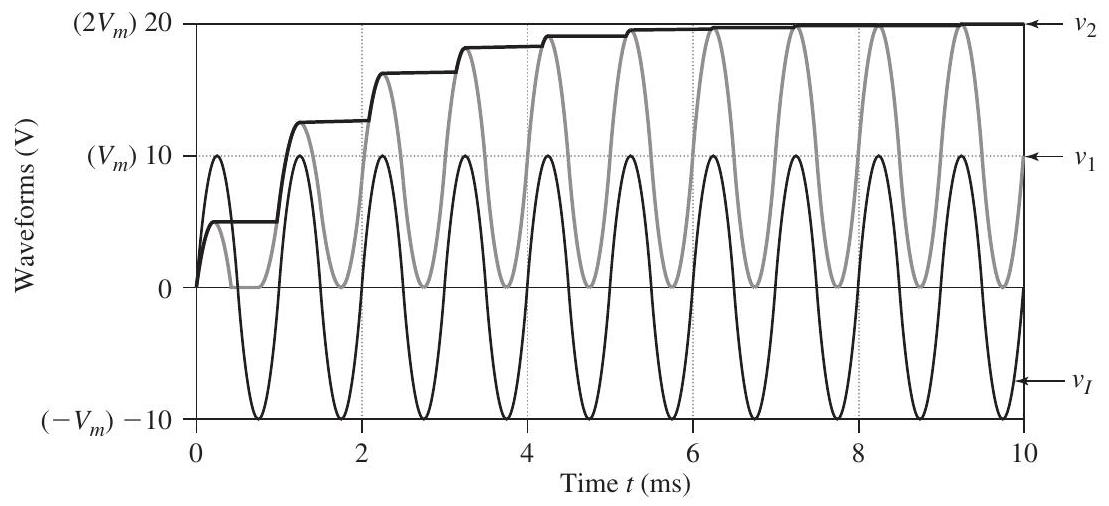
\includegraphics[max width=\textwidth, center]{2024_10_31_0c26dbfd3a789ec9acb1g-035}

FIGURE 1.24 Waveforms for the PSpice circuit of Fig. 1.23.

\section*{Exercise 1.3}
Denoting the value of $v_{2}$ following the $k$-th peak of $v_{I}$ as $v_{2}(k)$, use the charge conservation principle to show that $v_{2}(k)$ is related to the value $v_{2}(k-1)$ following the previous peak as

$$
v_{2}(k)=0.5 v_{2}(k-1)+10 \mathrm{~V}
$$

$k=2,3,4 \ldots$, and $v_{2}(1)=5 \mathrm{~V}$. At which peak of $v_{I}$ does $v_{2}$ come within about $10 \%$ of 20 V ? $1 \%$ of 20 V ?

Ans. For $10 \%, k=3$. For $1 \%, k=6$.\\
The principle at the basis of the voltage doubler can be generalized to achieve higher voltage-multiplication factors. Figure 1.25 shows a voltage quadrupler, whose waveforms are displayed in Fig. 1.26. We see again that after a transient situation lasting a certain number of cycles the output $v_{4}$ eventually settles to the dc value


\begin{equation*}
v_{4} \rightarrow 4 V_{m} \tag{1.8}
\end{equation*}


or $v_{4}=40 \mathrm{~V}$ in the present example. The reader is encouraged to trace through each waveform in detail to develop a feel for the workings of this clever circuit.

Voltage multipliers find application in integrated circuits, where it is desired to synthesize specific voltages to bias different on-chip circuits, starting out with a single supply voltage such as that provided by a rechargeable battery.\\
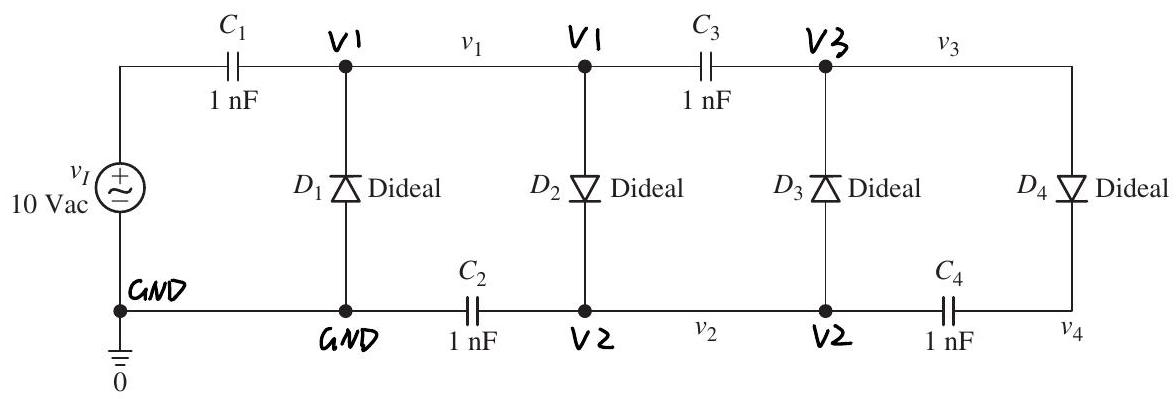
\includegraphics[max width=\textwidth, center]{2024_10_31_0c26dbfd3a789ec9acb1g-035(1)}

FIGURE 1.25 Voltage quadrupler.\\
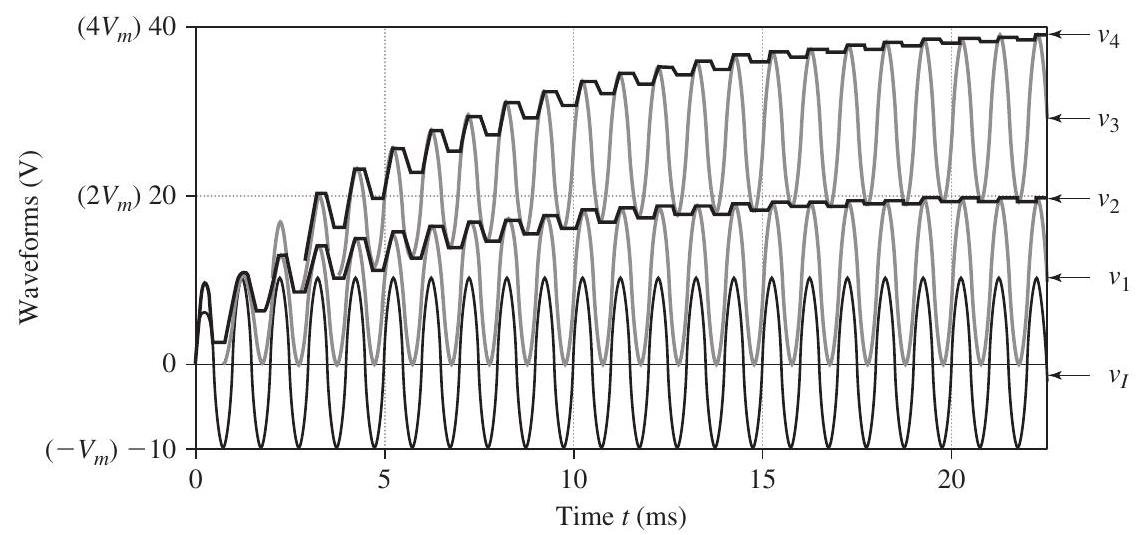
\includegraphics[max width=\textwidth, center]{2024_10_31_0c26dbfd3a789ec9acb1g-036}

FIGURE 1.26 Waveforms for the voltage quadrupler of Fig. 1.25.

\subsection*{1.3 OPERATIONAL AMPLIFIERS AND DIODE APPLICATIONS}
As we move along we shall find that the range of applications for diodes and, later, for transistors can be expanded significantly if we team up these devices with the operational amplifier, or op amp for short. Recall from prerequisite circuit courses that an op amp is a high-gain voltage amplifier that accepts two inputs, called the inverting input $v_{N}$ and the noninverting input $v_{P}$, and yields an output $v_{O}$ such that


\begin{equation*}
v_{O}=a\left(v_{P}-v_{N}\right) \tag{1.9}
\end{equation*}


where $a$ (in $\mathrm{V} / \mathrm{V}$ ) is the voltage gain (see Fig. 1.27a). In order to function, an op amp needs to be powered. Figure $1.27 a$ shows dual power supplies of $\pm V_{S}$, but a single supply is also common. (To reduce cluttering, it is customary to omit showing the supplies explicitly.) Physically, an op amp cannot swing $v_{O}$ above $+V_{S}$ or below $-V_{S}$. Overdriving it will simply cause $v_{O}$ to saturate at some voltage $V_{O H}$ in the vicinity of $+V_{S}$ or at some voltage $V_{O L}$ in the vicinity of $-V_{S}$, so Eq. (1.9) holds only so long as we confine $v_{O}$ within the range $V_{O L}<v_{O}<V_{O H}$, aptly called the linear output range. Figure $1.27 b$ shows the op amp's voltage transfer curve (VTC).

As we move along we shall find that the higher the voltage gain $a$, the better (as an example, the venerable 741 op amp has $a=200,000 \mathrm{~V} / \mathrm{V}$, also expressed as\\
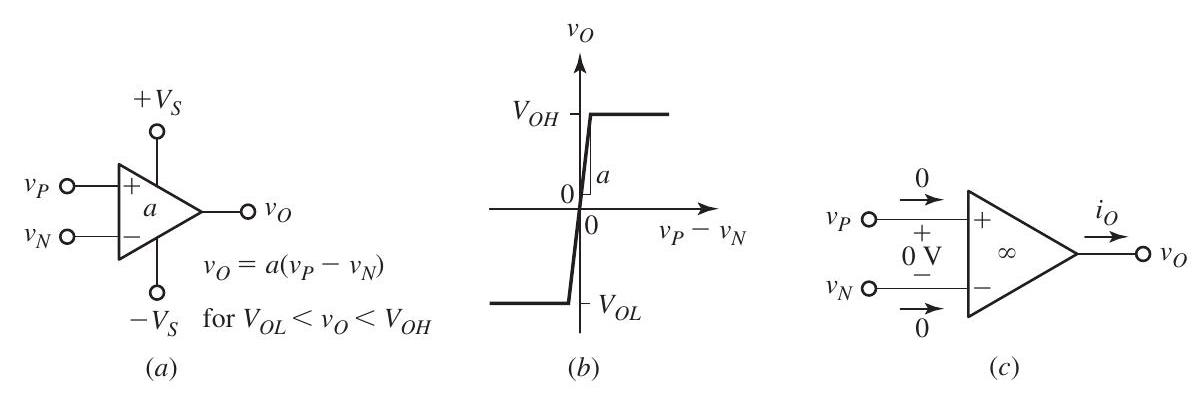
\includegraphics[max width=\textwidth, center]{2024_10_31_0c26dbfd3a789ec9acb1g-036(1)}

FIGURE 1.27 (a) Op amp symbol and labels. (b) The gain $a$ is the slope of the voltage transfer curve (VTC). (c) The input voltage of an ideal op amp approaches 0 V . Moreover, it draws no input currents.\\
$a=0.2 \mathrm{~V} / \mu \mathrm{V})$. Due to the sheer size of its gain, an op amp needs only a vanishingly small difference $v_{P}-v_{N}$ at the input to sustain a given voltage $v_{O}$ at the output (as an example, to sustain 1 V at the output, a 741 needs only $5 \mu \mathrm{~V}$ at the input!). Rewriting Eq. (1.9) as $\left(v_{P}-v_{N}\right)=v_{O} / a$, we get, in the ideal op amp limit of an infinitely high gain,

$$
\lim _{a \rightarrow \infty}\left(v_{P}-v_{N}\right)=\lim _{a \rightarrow \infty} \frac{v_{O}}{a}=0
$$

Op amps are designed to operate with negative feedback, an arrangement that allows the amplifier to influence its inverting input $v_{N}$ via an external network called the feedback network. With this viewpoint in mind, we express the above relation as


\begin{equation*}
\lim _{a \rightarrow \infty} v_{N}=v_{P} \tag{1.10}
\end{equation*}


which forms the basis of the important rule that engineers use to analyze op amp circuits:\\
Op Amp Rule: When given the ability to influence its own input $v_{N}$ via negative feedback, an ideal op amp will output whatever voltage $v_{O}$ and current $i_{O}$ it takes to force $v_{N}$ to track $v_{p}$. Moreover, the op amp will do this without drawing any current at either input pin (see Fig. 1.27c).

Let us put to use this rule to review the most popular op amp circuits.

\section*{Basic Op Amp Circuits}
The most popular op amp circuits are the noninverting amplifier, the inverting amplifier, the summing amplifier, and the voltage buffer.

\begin{itemize}
  \item The Noninverting Amplifier: In the circuit of Fig. $1.28 a$ the op amp influences $v_{N}$ via the voltage divider made up of $R_{1}$ and $R_{2}$ to give
\end{itemize}

$$
v_{N}=\frac{R_{1}}{R_{1}+R_{2}} v_{O}=\frac{v_{O}}{1+R_{2} / R_{1}}
$$

By the op amp rule we have $v_{N}=v_{P}\left(=v_{I}\right)$. Consequently, replacing $v_{N}$ with $v_{I}$ in the above expression and solving for the ratio $v_{O} / v_{I}$ gives


\begin{equation*}
A=\frac{v_{O}}{v_{I}}=1+\frac{R_{2}}{R_{1}} \tag{1.11}
\end{equation*}


\begin{center}
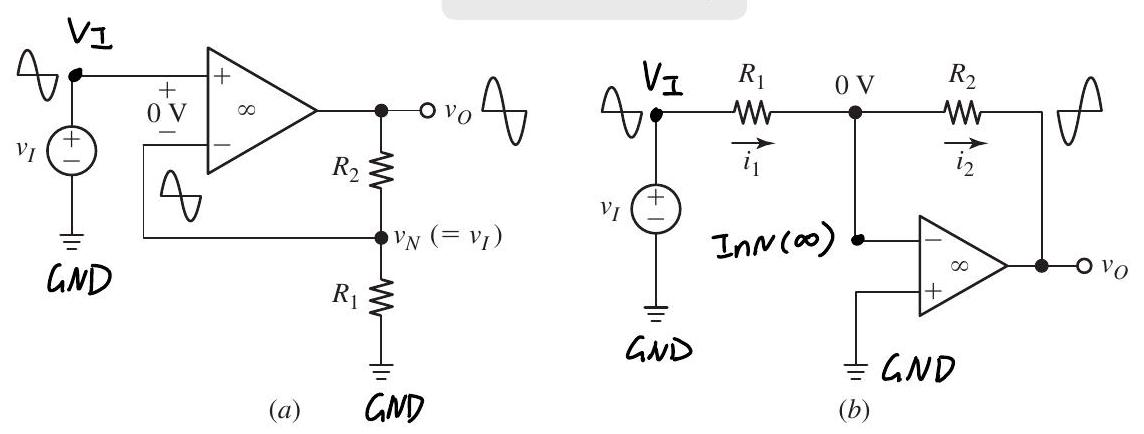
\includegraphics[max width=\textwidth]{2024_10_31_0c26dbfd3a789ec9acb1g-037}
\end{center}

FIGURE 1.28 (a) Noninverting and (b) inverting op amp configurations.\\
where $A$ represents the gain of the entire circuit (not to be confused with the gain $a(\rightarrow \infty)$ of the basic op amp). Since $v_{O}$ has the same polarity as $v_{I}$ the circuit is referred to as noninverting amplifier.

\begin{itemize}
  \item The Inverting Amplifier: In the circuit of Fig. $1.28 b$ the op amp influences $v_{N}$ via the feedback resistance $R_{2}$, and since the op amp rule implies $v_{N}=v_{P}=0$, we refer to node $v_{N}$ as a virtual ground. Any current injected by $v_{I}$ via $R_{1}$ is removed by $v_{O}$ via $R_{2}$, or $i_{1}=i_{2}$. Using Ohm's law,
\end{itemize}

$$
\frac{v_{I}-0}{R_{1}}=\frac{0-v_{O}}{R_{2}}
$$

Solving again for the ratio $v_{O} / v_{I}$ gives


\begin{equation*}
A=\frac{v_{O}}{v_{I}}=-\frac{R_{2}}{R_{1}} \tag{1.12}
\end{equation*}


Since the polarity of $v_{O}$ is opposite to that of $v_{I}$ the circuit is called an inverting amplifier.

\begin{itemize}
  \item The Summing Amplifier: By the op amp rule, the inverting-input node in Fig. 1.29 is at virtual ground. This node is called a summing junction because it sums the currents coming from the input sources $v_{1}$ and $v_{2}$ and diverts this sum to the output node $v_{O}$ to give
\end{itemize}

$$
\frac{v_{1}-0}{R_{1}}+\frac{v_{2}-0}{R_{2}}=\frac{0-v_{0}}{R_{3}}
$$

Solving for $v_{o}$,


\begin{equation*}
v_{O}=-\left(\frac{R_{3}}{R_{1}} v_{1}+\frac{R_{3}}{R_{2}} v_{2}\right) \tag{1.13}
\end{equation*}


If $R_{1}=R_{2}$, the circuit gives $v_{O}=-\left(R_{3} / R_{1}\right)\left(v_{1}+v_{2}\right)$ and is aptly called a summing amplifier.

\begin{itemize}
  \item The Voltage Buffer: Letting $R_{2}=0$ and $R_{1}=\infty$ in the circuit of Fig. $1.28 a$ turns it into a unity-gain amplifier $(A=1 \mathrm{~V} / \mathrm{V})$. Its main application is as a voltage buffer to eliminate inter-stage loading. As an example, consider Fig. 1.30a, where a signal\\
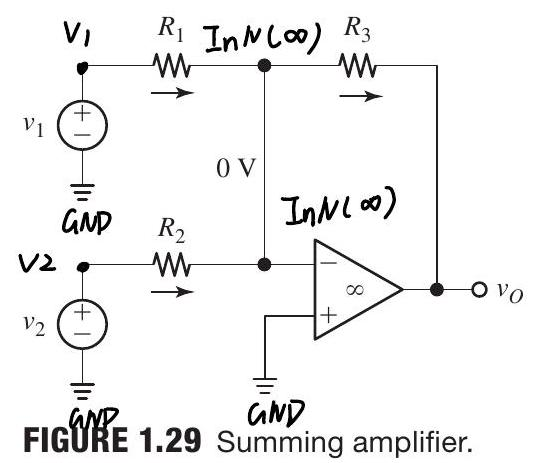
\includegraphics[max width=\textwidth, center]{2024_10_31_0c26dbfd3a789ec9acb1g-038}\\
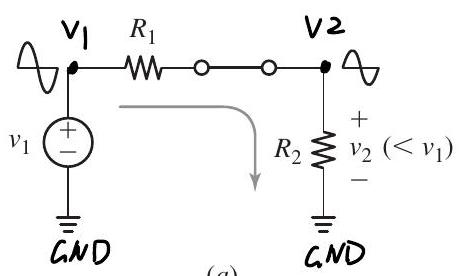
\includegraphics[max width=\textwidth, center]{2024_10_31_0c26dbfd3a789ec9acb1g-039(3)}\\
(a)\\
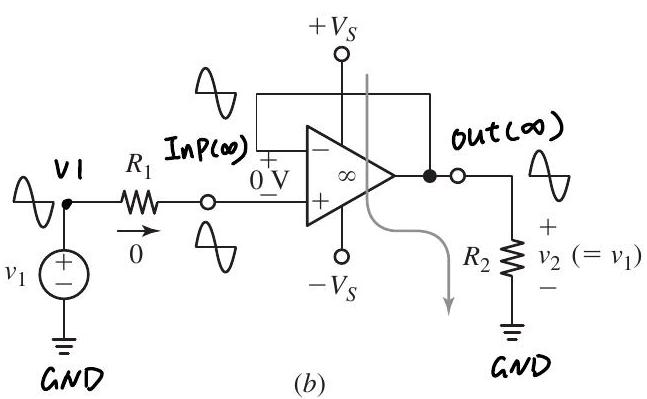
\includegraphics[max width=\textwidth, center]{2024_10_31_0c26dbfd3a789ec9acb1g-039(2)}
\end{itemize}

FIGURE 1.30 Using a unity-gain voltage buffer to eliminate loading (current polarities shown for $v_{1}>0$ ).\\
source $v_{1}$ with internal resistance $R_{1}$ is to be fed to a load $R_{2}$. If we connect the source to the load via a plain wire, $R_{2}$ will form a voltage divider with $R_{1}$, giving $v_{2}=$ $v_{1} /\left(1+R_{1} / R_{2}\right)$. Clearly $v_{2}$ is less than $v_{1}$, a situation referred to as loading and stemming from the fact that $R_{2}$ draws current via $R_{1}$, so there is voltage loss across $R_{1}$.

However, if we couple the source to the load via a buffer as in Fig. 1.30b, there will be no voltage drop across $R_{1}$ because the op amp is designed to draw no input currents. Consequently the buffer eliminates loading to give $v_{2}=v_{1}$. Of course $R_{2}$ does draw current, but this is supplied by the op amp, which in turn draws it from the power supply $+V_{S}$ rather than from $v_{1}$. (The illustration refers to the case $v_{1}>0$; for $v_{1}<0$ the load current will flow from $R_{2}$ through the op amp to $-V_{S}$.)

The above configurations show up so often, either on their own or as subcircuits of more complex systems, that we shall apply Eqs. (1.10) through (1.13) quite frequently.

\section*{Our First Diode/Op-Amp Circuit}
Having reviewed op amp basics, we are now ready to investigate our first diode/opamp circuit, shown in Fig. 1.31a. Where do we begin? As a rule, start out using simple inspection to see if you can identify already familiar subcircuits, and then build up your understanding from there, one step at a time. In the present case we observe that $D_{2}$ and $R_{3}$ form a half-wave rectifier of the type of Fig. 1.10a, so we can follow the line of reasoning developed there and analyze the cases $v_{I}>0$ and $v_{I}<0$ separately.\\
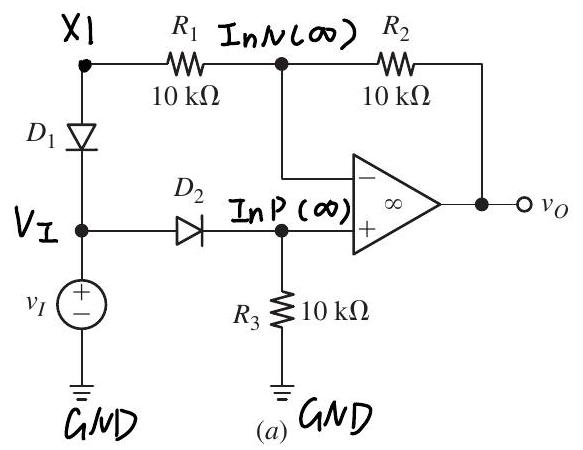
\includegraphics[max width=\textwidth, center]{2024_10_31_0c26dbfd3a789ec9acb1g-039}\\
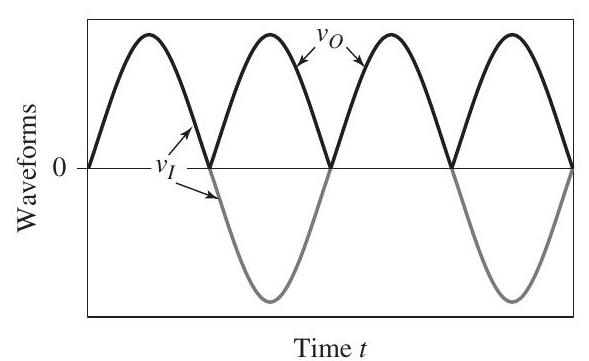
\includegraphics[max width=\textwidth, center]{2024_10_31_0c26dbfd3a789ec9acb1g-039(1)}\\
(b)

FIGURE 1.31 (a) Our first diode/op-amp circuit, and (b) its input and output waveforms.\\
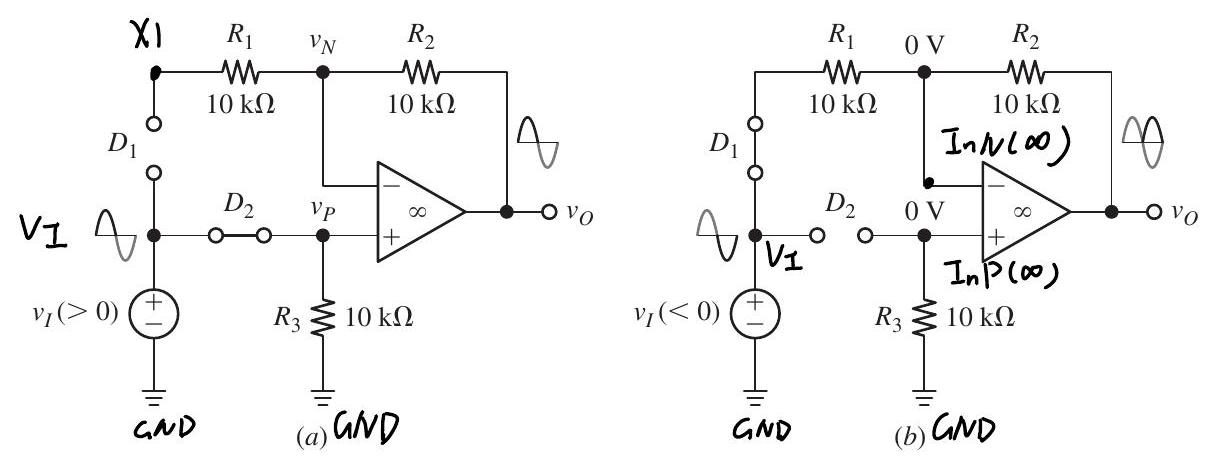
\includegraphics[max width=\textwidth, center]{2024_10_31_0c26dbfd3a789ec9acb1g-040}

FIGURE 1.32 Redrawing the circuit of Fig. 1.31a for (a) $v_{l}>0$ and (b) $v_{l}<0$.

\begin{itemize}
  \item For $v_{I}>0, D_{2}$ is on, making $v_{P}=v_{I}$. But, by the op amp rule we have $v_{N}=v_{P}$, and thus $v_{N}=v_{I}$. This causes $D_{1}$ to be off, as pictured in Fig. 1.32a. In the absence of any current through $R_{2}$ the op amp gives $v_{O}=v_{N}$, so
\end{itemize}


\begin{equation*}
v_{O}=v_{I} \tag{1.14a}
\end{equation*}


\begin{itemize}
  \item For $v_{I}<0, D_{2}$ is off, making $v_{P}=0$ and thus, by the op amp rule, $v_{N}=0 . D_{1}$ is now on, as pictured in Fig. 1.32b, and the op amp acts as an inverting amplifier to give
\end{itemize}


\begin{equation*}
v_{O}=-\frac{R_{2}}{R_{1}} v_{I}=-\frac{10}{10} v_{I}=-v_{I} \tag{1.14b}
\end{equation*}


\begin{itemize}
  \item We combine the two expressions by writing
\end{itemize}


\begin{equation*}
v_{O}=\left|v_{I}\right| \tag{1.15}
\end{equation*}


and by stating that the circuit is a full-wave rectifier. The function is similar to that provided by the circuit of Fig. 1.12a and graphed in Fig. 1.13. There is a difference, however: in the circuit of Fig. 1.12a the rectified signal appears across a floating load, whereas in the op amp version of Fig. 1.31a the rectified signal is referenced to ground and as such it can be applied to a grounded load.

\section*{Exercise 1.4}
Find $v_{O}$ in the circuit of Fig. 1.31a if (a) $R_{3}$ is doubled; (b) $R_{2}$ is doubled; (c) $R_{1}$ is doubled; (d) the direction of each diode is reversed; (e) only the direction of $D_{1}$ is reversed.

Ans. (a) $v_{O}=\left|v_{I}\right| ;$ (b) $v_{O}=v_{I}$ for $v_{I}>0 ; v_{O}=-2 v_{I}$ for $v_{I}<0 ;$ (c) $v_{O}=v_{I}$ for $v_{I}>0$, $v_{O}=-0.5 v_{I}$ for $v_{I}<0 ;(d) v_{O}=-\left|v_{I}\right| ;(e) v_{O}=v_{I}$ for $v_{I}>0, v_{O}=0$ for $v_{I}<0$.

\subsection*{1.4 SEMICONDUCTORS}
The material in widest use by the semiconductor industry today is silicon $(\mathrm{Si})$, an element of Group IV of the periodic table of elements (see the portion shown in Table 1.1). The atoms of Group IV elements possess four electrons in their outer electron shell, also called the valence band. Each atom shares these four electrons with its four nearest neighbor atoms to form covalent bonds. These bonds keep atoms

TABLE 1.1 Portion of the Periodic Table with the most common semiconductor and dopant elements.

\begin{center}
\begin{tabular}{l|l|l}
\hline
III & IV & V \\
\hline
5 & 6 & 7 \\
B & $\mathbf{C}$ & $\mathbf{N}$ \\
Boron & Carbon & Nitrogen \\
\hline
13 & 14 & 15 \\
Al & $\mathbf{S i}$ & $\mathbf{P}$ \\
Aluminum & Silicon & Phosphorus \\
\hline
31 & 32 & 33 \\
Ga & $\mathbf{G e}$ & As \\
Gallium & Germanium & Arsenic \\
\hline
49 & 50 & 51 \\
In & Sn & Sb \\
Indium & Tin & Antimony \\
\hline
\end{tabular}
\end{center}

bound to fixed positions of an orderly spatial structure known as crystal lattice. This is depicted in the two-dimensional rendition of Fig. 1.33a. The number of silicon atoms per unit volume (atoms $/ \mathrm{cm}^{3}$ ), also called atomic density, is


\begin{equation*}
N_{s i}=5 \times 10^{22} \text { atoms } / \mathrm{cm}^{3} \tag{1.16}
\end{equation*}


Due to thermal agitation, a covalent bond may break on occasion, freeing an electron which then becomes available for conduction. Consequently, the parent atom is said to be ionized. As we know, the electron charge is $-q$, where


\begin{equation*}
q=1.602 \times 10^{-19} \mathrm{C} \tag{1.17}
\end{equation*}


Once an electron moves away from a covalent site, it leaves behind a vacancy having charge $+q$, as shown in Fig. 1.33b. An electron from another covalent bond may fill this vacancy, leaving in turn behind another vacancy at the covalent site of origin.\\
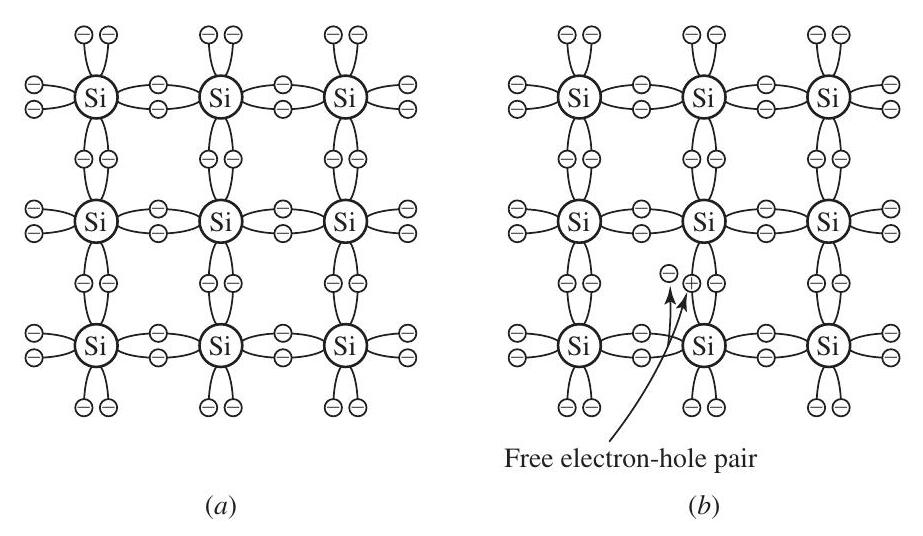
\includegraphics[max width=\textwidth, center]{2024_10_31_0c26dbfd3a789ec9acb1g-041}

FIGURE 1.33 (a) Pure silicon. (b) Creation of an electron-hole pair by thermal agitation.

As this process repeats itself, we are in effect witnessing the motion of positively charged vacancies, or holes, through the crystal.

Just as thermal agitation results in the creation of free electron-hole pairs, an electron and a hole may recombine and thus disappear from the pool of free charges. The recombination rate is proportional to the number of free electron-hole pairs available, which in turn is a strong function of temperature. In thermal equilibrium, the recombination rate equals the generation rate, resulting in an equilibrium electron concentration (or density) $n$ (electrons/cm ${ }^{3}$ ) and hole concentration (or density) $p$ (holes $/ \mathrm{cm}^{3}$ ) such that


\begin{equation*}
n=p=n_{i} \tag{1.18}
\end{equation*}


where $n_{i}$ is called the intrinsic concentration. For silicon, $n_{i}$ is such that


\begin{equation*}
n_{i}^{2}(T)=B T^{3} e^{-V_{c 0} / V_{T}} \mathrm{~cm}^{-6} \tag{1.19}
\end{equation*}


where $T$ is absolute temperature, in $\mathrm{K}, B$ is a suitable constant, $V_{G 0}=1.205 \mathrm{~V}$ is the bandgap voltage for silicon, and


\begin{equation*}
V_{T}=\frac{k T}{q} \tag{1.20}
\end{equation*}


is a temperature-dependent scaling factor, in V, often arising in semiconductor physics and called the thermal voltage. Here $q$ is the electron charge and $k=1.381 \times 10^{-23} \mathrm{~J} / \mathrm{K}$ is Boltzmann's constant. At room temperature ( $T=300 \mathrm{~K}$ ), we have $V_{T}=25.86 \mathrm{mV}$ $\cong 26 \mathrm{mV}$ 。

For silicon, Eq. (1.19) takes on the form


\begin{equation*}
n_{i}^{2}(T)=1.5 \times 10^{33} T^{3} e^{-14,028 / T} \mathrm{~cm}^{-6} \tag{1.21}
\end{equation*}


We observe that $n_{i}$ is a strong function of temperature. At $T=300 \mathrm{~K}$ we have $n_{i}^{2}=2 \times 10^{20} \mathrm{~cm}^{-6}$, or $n_{i}=1.4 \times 10^{10} / \mathrm{cm}^{3}$, indicating that only one in about $36 \times$ $10^{12}$ silicon atoms is ionized. By contrast, in a good conductor each atom contributes one or more electrons to conduction. It is apparent that at room temperature pure silicon is not much of a conductor.

\section*{Doping}
The electric properties of an element of Group IV can be altered dramatically by replacing some of its atoms with atoms of elements from the adjacent groups. For instance, replacing an atom of silicon with one of phosphorous $(\mathrm{P})$, which belongs to Group V and thus possesses five electrons in its outer shell, results in the situation of Fig. 1.34a. Four of the five electrons will go into forming covalent bonds, just like those of a silicon atom would; the fifth electron, due to thermal agitation, will wander throughout the crystal, no longer belonging to any particular atom and thus being free and available for conduction. Group V elements are referred to as donors in that each atom contributes, or donates, an electron to the silicon crystal. By contrast, replacing an atom of silicon with one of boron (B), which belongs to\\
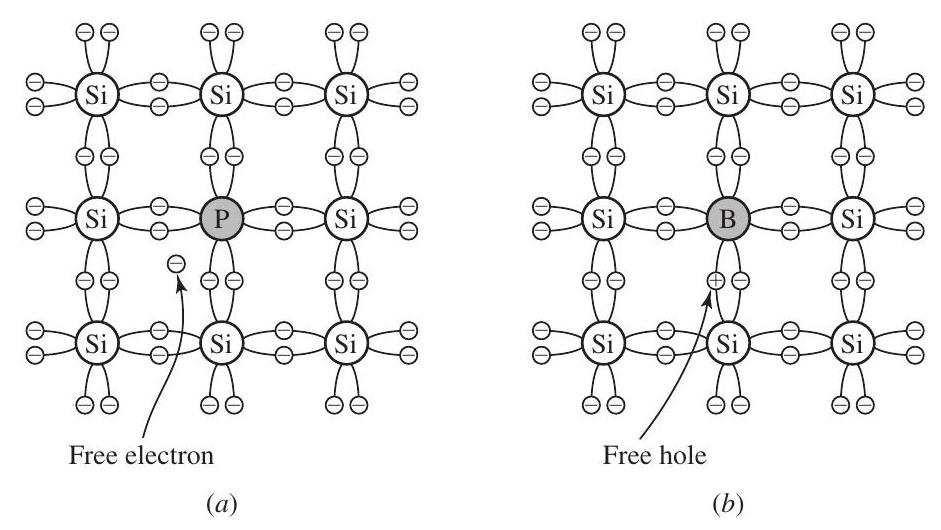
\includegraphics[max width=\textwidth, center]{2024_10_31_0c26dbfd3a789ec9acb1g-043}

FIGURE 1.34 Silicon with (a) a donor atom, and (b) an acceptor atom.

Group III and thus possesses only three electrons in its outer shell, will lead to the situation of Fig. 1.34b. Here, the lack of a fourth electron results in a hole, and since holes in turn accept electrons when they recombine, Group III elements are referred to as acceptors.

The replacement of silicon atoms with donor or acceptor atoms is called doping. Since doped silicon is no longer pure, donor and acceptor atoms are collectively referred to as impurities. By doping silicon with a sufficient number of impurities, we can turn it into a good conductor-hence the reason for calling it a semiconductor. Doping can be achieved in more than one way. With solid-state diffusion, the doping material is deposited on a selected area of the silicon crystal, which is then placed in a high temperature furnace to force the impurity atoms to penetrate and diffuse into the underlying region of the crystal. With ion implantation, the silicon crystal is bombarded with ions of the desired impurity material, which then remain embedded in the crystal. Doped silicon can also be grown directly as a crystal, starting with a suitable mixture of silicon and impurity atoms of the desired type.

The donor and acceptor concentrations (atoms $/ \mathrm{cm}^{3}$ ), also called doping densities, are denoted as $N_{D}$ and $N_{A}$, respectively. Depending on the particular requirements, doping doses may range from as low as $10^{14}$ atoms $/ \mathrm{cm}^{3}$ to as high as $10^{21}$ atoms $/ \mathrm{cm}^{3}$, that is, practical impurity densities are always much higher than the room-temperature intrinsic electron-hole concentration ( $\left.n_{i}=1.4 \times 10^{10} / \mathrm{cm}^{3}\right)$. Consequently, at room temperature, silicon doped with donor impurities, also called $n$-type silicon, has $n>$ $N_{D}$, while silicon doped with acceptor impurities, also called p-type silicon, has $p>N_{A}$.

Regardless of the type and amount of doping, the electron and hole concentrations satisfy at all times the mass-action law,


\begin{equation*}
n \times p=n_{i}^{2} \tag{1.22}
\end{equation*}


or $n \times p=2 \times 10^{20} \mathrm{~cm}^{-6}$ at room temperature ( $T=300 \mathrm{~K}$ ). Consequently, in n-type silicon we have


\begin{equation*}
n \cong N_{D} \quad p \cong \frac{n_{i}^{2}}{N_{D}} \tag{1.23a}
\end{equation*}


while in p-type silicon we have


\begin{equation*}
p \cong N_{A} \quad n \cong \frac{n_{i}^{2}}{N_{A}} \tag{1.23b}
\end{equation*}


To put numbers in perspective, suppose some $n$-type silicon has been doped with $N_{D}=10^{16} / \mathrm{cm}^{3}$. Then, $n \cong 10^{16} / \mathrm{cm}^{3}$ and $p \cong 2 \times 10^{20} / 10^{16}=2 \times 10^{4} / \mathrm{cm}^{3}$, indicating a material much richer in electrons and much poorer in holes than intrinsic silicon. Since $n \gg p$, electrons in $n$-type silicon are aptly called majority charge carriers, and holes minority charge carriers. Conversely, a $p$-type silicon with $N_{A}=10^{18} / \mathrm{cm}^{3}$ would have $p \cong 10^{18} / \mathrm{cm}^{3}$ and $n \cong 2 \times 10^{2} / \mathrm{cm}^{3}$. Since now $p \gg n$, the majority carriers in $p$-type silicon are holes, and the minority carriers are electrons.

It is understood that the thermal generation of electron-hole pairs continues to take place just as in the intrinsic case. However, with such an abundance of majority carriers, the chance of recombining for minority carriers is now much higher, this being the reason for their much reduced concentration. In fact, the balance between the two charge types is governed by the mass-action law!

We note that the designations $n$-type and $p$-type identify only the type of majority carriers in the given material. They should not mislead the reader into regarding $n$-type material as negatively charged, or $p$-type material as positively charged! Regardless of the doping type, the material remains at all times neutrally charged because for every charge that has been freed there is the charge of the ionized atom left behind, which is of the opposite polarity. Figure. 1.35 depicts $n$ and $p$ for three significant cases.

\section*{Drift and Diffusion Currents}
There are two types of conduction mechanisms in semiconductors, often coexisting: drift and diffusion.

\begin{itemize}
  \item The Drift Current: To discuss the drift mechanism, refer to Fig. 1.36a, top, where a slab of $p$-type material is assumed to be immersed in an electric field of strength $E$ (in $\mathrm{V} / \mathrm{cm}$ ). Such a field can be produced by connecting an external battery across the slab. If the slab is homogeneous, as assumed here, the\\
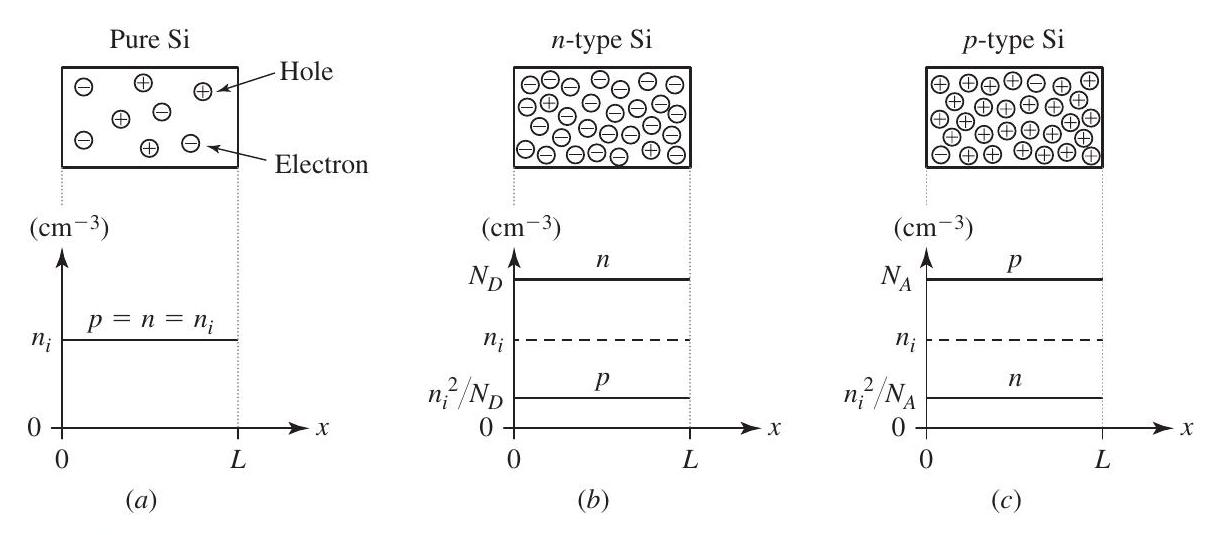
\includegraphics[max width=\textwidth, center]{2024_10_31_0c26dbfd3a789ec9acb1g-044}
\end{itemize}

FIGURE 1.35 Mobile-charge concentrations in a slab of (a) pure silicon, (b) n-type silicon, and (c) p-type silicon. (The vertical scales are logarithmic.)\\
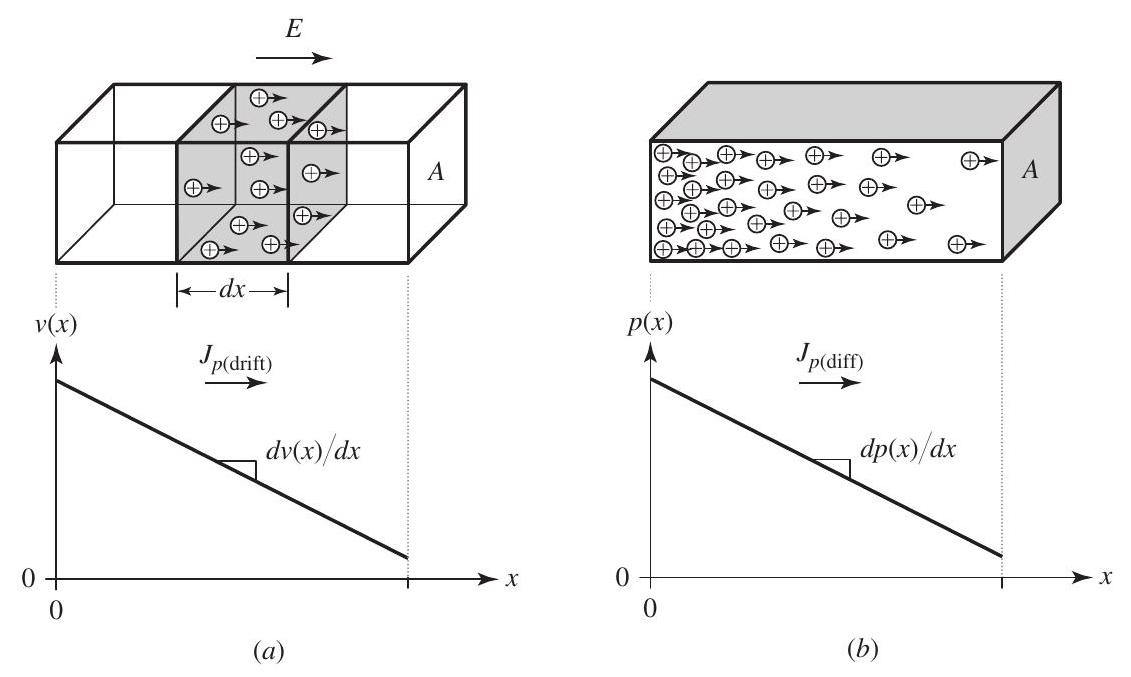
\includegraphics[max width=\textwidth, center]{2024_10_31_0c26dbfd3a789ec9acb1g-045}

FIGURE 1.36 Illustrating (a) current drift and (b) current diffusion for the case of holes.\\
potential $v(x)$ will vary linearly across the slab, as shown at the bottom. From basic physics we know that field and potential are related as


\begin{equation*}
E=-\frac{d v(x)}{d x} \tag{1.24}
\end{equation*}


Consequently, $E$ will be constant throughout the homogeneous slab.\\
Now, under the accelerating effect of $E$, holes will drift in the same direction as the field and achieve an average drift velocity $v_{p}$ (in $\mathrm{cm} / \mathrm{s}$ ) which is linearly proportional to the field strength,


\begin{equation*}
v_{p}=\mu_{p} E \tag{1.25a}
\end{equation*}


Aptly called the hole mobility, $\mu_{p}$ (in $\mathrm{cm}^{2} / \mathrm{Vs}$ ) gives a measure of the average drift velocity acquired by holes for a given applied field. As holes drift, they produce the current $i_{p(\text { drift })}=d Q_{p} / d t$, where $d Q_{p}$ is the amount of charge transferred during the interval $d t$. Given that during $d t$ holes travel the distance $d x=v_{p} d t$, the holes making up $d Q_{p}$ are contained within the volume $A d x=A v_{p} d t$, and their number is thus $p A v_{p} d t$, where $p$ is their concentration (holes $/ \mathrm{cm}^{3}$ ), and $A$ is the cross sectional area of the silicon slab (in $\mathrm{cm}^{2}$ ). Multiplying this number by the hole charge $+q$ gives $d Q_{p}=q p A v_{p} d t$, so

$$
i_{p(\mathrm{drift})}=\frac{d Q_{p}}{d t}=q p A v_{p}=q p A \mu_{p} E
$$

As we progress, we will find it more convenient to work with the current per unit area, or current densiy $J$ (in $\mathrm{A} / \mathrm{cm}^{2}$ ), rather than with the ordinary current $i$ (in A). The hole drift current density is simply $J_{p(\text { drift })}=i_{p(\text { drift })} / A$, or


\begin{equation*}
J_{p(\mathrm{drift})}=q p \mu_{p} E \tag{1.25b}
\end{equation*}


Similar considerations hold for a slab of $n$-type material, except that in this case the mobile charges are electrons, whose concentration and mobility are $n$ and $\mu_{n}$. Thus, the average drift velocity of electrons is


\begin{equation*}
v_{n}=\mu_{n} E \tag{1.26a}
\end{equation*}


where $\mu_{n}$ (in $\mathrm{cm}^{2} / \mathrm{Vs}$ ) is the electron mobility, and the electron drift current density is


\begin{equation*}
J_{n(\mathrm{drift})}=q n \mu_{n} E \tag{1.26b}
\end{equation*}


Equation (1.26b) is also at the basis of metals and ordinary conductors such as composition resistors, where the only type of mobile charges available are electrons. Both equations indicate the necessary ingredients for good conduction: high concentration along with high mobility.

\begin{itemize}
  \item The Diffusion Current: The other mechanism for charge-carrier motion in semiconductors is diffusion-a mechanism not found in ordinary conductors. As we progress, we shall see that in semiconductor devices it is possible to establish and continuously maintain non-uniform profiles for the mobile charge densities. Figure $1.36 b$ shows an example of a linear density profile, such as that found in the base region of a forward-biased bipolar junction transistor. As holes wander randomly because of thermal agitation, they tend to diffuse from regions of higher density to regions of lower density, or toward the right in our example. This is similar to particles of smoke diffusing from the smoking area to the rest of a room. If holes are continuously injected to the left while being removed from the right, a sustained current flow will result. The hole diffusion current density is
\end{itemize}


\begin{equation*}
J_{p(\mathrm{diff})}=-q D \frac{d p(x)}{d x} \tag{1.27a}
\end{equation*}


where $D_{p}$ is the hole diffusivity (in $\mathrm{cm}^{2} / \mathrm{s}$ ). The negative sign stems from the fact that holes flow in the direction of the negative gradient in $p$. Likewise, the electron diffusion current density is


\begin{equation*}
J_{n(\mathrm{diff})}=q D_{n} \frac{d n(x)}{d x} \tag{1.27b}
\end{equation*}


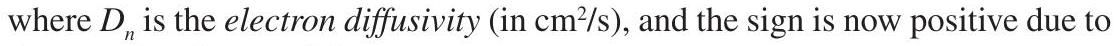
\includegraphics[max width=\textwidth]{2024_10_31_0c26dbfd3a789ec9acb1g-046} the negative charge of electrons.

We note strong similarities between the expressions for the drift and diffusion currents. In fact, substituting Eq. (1.24) into Eqs. (1.25b) and (1.26b) gives

$$
J_{p(\mathrm{drift})}=-q p \mu_{p} \frac{d v(x)}{d x} \quad J_{n(\mathrm{drift})}=q n \mu \frac{d v(x)}{d x}
$$

\begin{center}
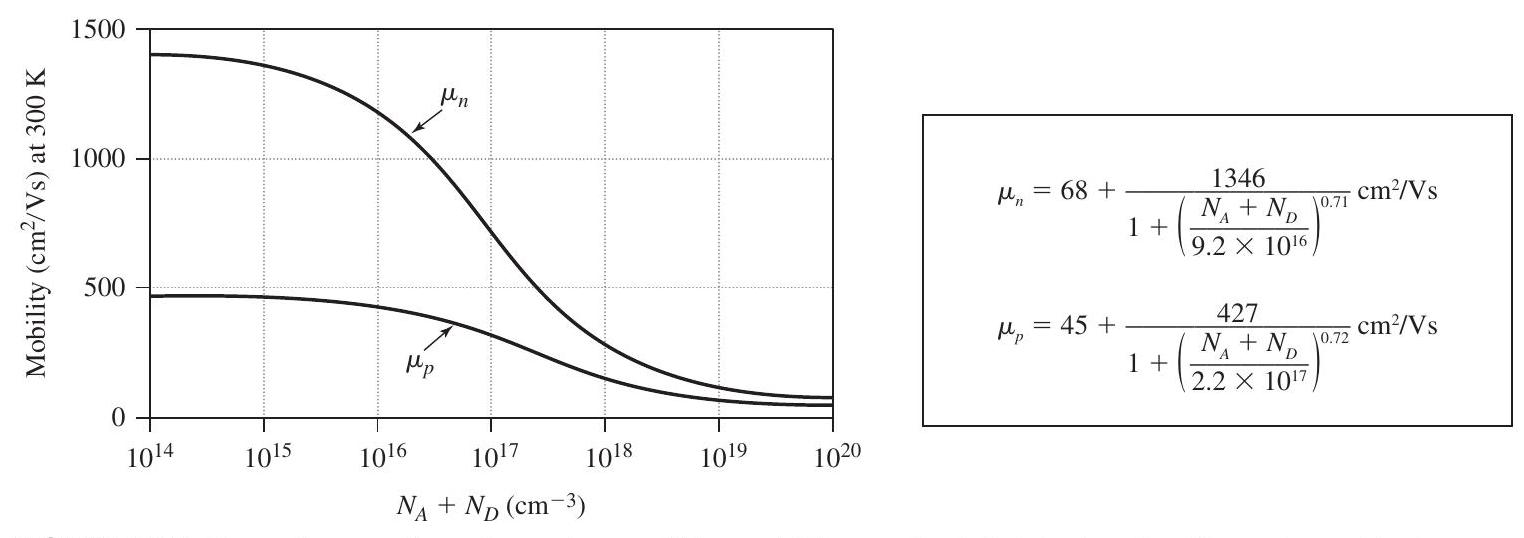
\includegraphics[max width=\textwidth]{2024_10_31_0c26dbfd3a789ec9acb1g-047}
\end{center}

FIGURE 1.37 Room-temperature dependence of the mobilities on the total doping density, and empirical formulas for their calculation for the case of donor atoms of phosphorous and acceptor atoms of boron.\\
which are even closer in form to Eqs. (1.27a) and (1.27b). These equations indicate that:

\begin{itemize}
  \item To sustain a given current we need a gradient (a voltage gradient to sustain drift, a density gradient to sustain diffusion).
  \item Charge flow is in the direction of a decreasing gradient.
  \item The diffusivities $D_{p}$ and $D_{n}$ play a similar role to the mobilities $\mu_{p}$ and $\mu_{n}$ in that each offers a measure of how much current stems from a given gradient. Indeed, it turns out that diffusivities and mobilities are related by Einstein's relations
\end{itemize}


\begin{equation*}
\frac{D_{n}}{\mu_{n}}=\frac{D_{p}}{\mu_{p}}=V_{T} \tag{1.28}
\end{equation*}


where $V_{T} \cong 26 \mathrm{mV}$ is the thermal voltage of Eq. (1.20).\\
Mobilities and diffusivities are greatest when silicon is pure, but decrease with doping as well as temperature. Figure 1.37 shows the dependence of $\mu_{n}$ and $\mu_{p}$ on the total doping density $\left(N_{A}+N_{D}\right)$, at room temperature. The higher mobility (by a factor of two to three) exhibited by electrons compared to holes is the primary reason why $n$-type materials are generally preferred over $p$-type materials, particularly in the fabrication of devices intended for high-speed operation.

Lastly, it must be pointed out that the linear relationships between velocities and electric field, expressed as $v_{n}=\mu_{n} E$ and $v_{p}=\mu_{p} E$, hold only up to a certain field strength, typically on the order of $5 \mathrm{kV} / \mathrm{cm}$. Past this limit, electron and hole velocities saturate at approximately $10^{7} \mathrm{~cm} / \mathrm{s}$. Aptly called velocity saturation, this phenomenon sets an upper limit on the speed of operation of semiconductor devices such as MOSFETs.

\section*{An Example: The Integrated-Circuit Diode}
Figure 1.38 illustrates the most basic steps involved in the fabrication of the pn junction diode, a semiconductor device at the basis of most other integrated-circuit (IC) devices. Starting out with a lightly doped $n$-type slab, such as $N_{D}=10^{15} / \mathrm{cm}^{3}$, a localized boron diffusion is made to create a $p$-type region. Clearly, in order to overcome\\
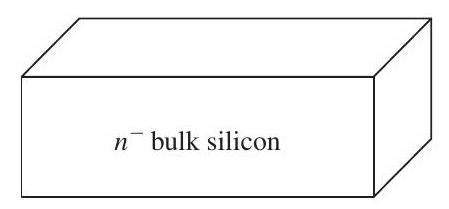
\includegraphics[max width=\textwidth, center]{2024_10_31_0c26dbfd3a789ec9acb1g-048(1)}\\
(a)\\
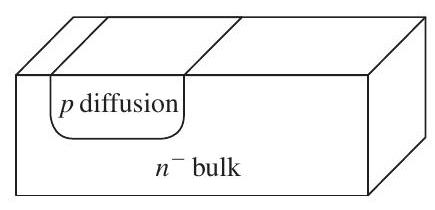
\includegraphics[max width=\textwidth, center]{2024_10_31_0c26dbfd3a789ec9acb1g-048(2)}\\
(b)\\
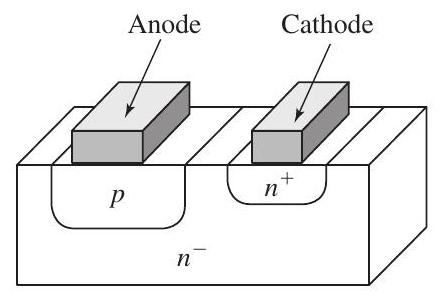
\includegraphics[max width=\textwidth, center]{2024_10_31_0c26dbfd3a789ec9acb1g-048}\\
(c)

FIGURE 1.38 Basic fabrication steps of an IC diode: (a) starting material, (b) p-type diffusion, and (c) provision for its connection to the outside.\\
the existing $n$-type nature of this region, the acceptor density $N_{A}$ must exceed the existing donor density $N_{D}$ there. Then, in this region we have

$$
p \cong N_{A}-N_{D} \quad n \cong \frac{n_{i}^{2}}{N_{A}-N_{D}}
$$

An additional diffusion is made to create a heavily doped $n$-type region to ensure an ohmic contact between the $n$-type slab and a metal (more on this later in the chapter), and finally metal depositions are made to allow for the interconnection of the device to external circuitry.

The dimensions of the above device are in the range of micro meters $\left(1 \mu \mathrm{~m}=10^{-6} \mathrm{~m}\right)$. Such tiny dimensions allow for the simultaneous fabrication of a very large number of devices on the same wafer. To prevent different devices from interfering with each other, we must keep them electrically isolated from each other. Interestingly enough, a popular way of achieving isolation is through additional reverse-biased pn junctions, a subject that we will illustrate in greater detail when studying the fabrication of transistors. The interested student is encouraged to search the Web for videos and articles illustrating the fascinating subject of integrated circuit fabrication.

Find the electron and hole concentrations $n$ and $p$ as well as the mobilities $\mu_{n}$ and $\mu_{p}$, and the diffusivities $D_{n}$ and $D_{p}$ in the three regions of the structure of Fig. 1.38, assuming the following doping densities:\\
(a) $n^{-}$-type bulk: $N_{D}=10^{15}$ phosphorous atoms $/ \mathrm{cm}^{3}$\\
(b) $p$-type diffusion: $N_{A}=10^{17}$ boron atoms $/ \mathrm{cm}^{3}$\\
(c) $n^{+}$-type diffusion: $N_{D}=10^{20}$ phosphorous atoms $/ \mathrm{cm}^{3}$

\section*{Solution}
(a) We have $n \cong N_{D}=10^{15} / \mathrm{cm}^{3}$ and $p \cong n_{i}^{2} / N_{D}=2 \times 10^{20} / 10^{15}=2 \times 10^{5} / \mathrm{cm}^{3}$. Using the empirical formulas of Fig. 1.37, we find

$$
\begin{aligned}
& \mu_{n}=68+\frac{1346}{1+\left(\frac{10^{15}}{9.2 \times 10^{16}}\right)^{0.71}}=1362 \mathrm{~cm}^{2} / \mathrm{Vs} \\
& \mu_{p}=45+\frac{427}{1+\left(\frac{10^{15}}{2.2 \times 10^{17}}\right)^{0.72}}=463 \mathrm{~cm}^{2} / \mathrm{Vs}
\end{aligned}
$$

Using Eq. (1.28), we find $D_{n}=0.026 \times 1362=35.4 \mathrm{~cm}^{2} / \mathrm{s}$ and $D_{p}=$ $0.026 \times 463=12 \mathrm{~cm}^{2} / \mathrm{s}$.\\
(b) We now have $p \cong N_{A}-N_{D}=10^{17}-10^{15} \cong 10^{17} / \mathrm{cm}^{3}$ and $n \cong n_{i}^{2} /\left(N_{A}-N_{D}\right) \cong$ $2 \times 10^{3} / \mathrm{cm}^{3}$. Using again the empirical formulas,

$$
\begin{aligned}
& \mu_{n}=68+\frac{1346}{1+\left(\frac{10^{17}+10^{15}}{9.2 \times 10^{16}}\right)^{0.71}}=719 \mathrm{~cm}^{2} / \mathrm{Vs} \\
& \mu_{p}=45+\frac{427}{1+\left(\frac{10^{17}+10^{15}}{2.2 \times 10^{17}}\right)^{0.72}}=317 \mathrm{~cm}^{2} / \mathrm{Vs}
\end{aligned}
$$

Moreover, $D_{n}=0.026 \times 719=18.7 \mathrm{~cm}^{2} / \mathrm{s}$ and $D_{p}=8.3 \mathrm{~cm}^{2} / \mathrm{s}$.\\
(c) We now have $n \cong 10^{20}+10^{15} \cong 10^{20} / \mathrm{cm}^{3}, p \cong 2 / \mathrm{cm}^{3} ; \mu_{n}=78 \mathrm{~cm}^{2} / \mathrm{Vs}$, $D_{n}=2 \mathrm{~cm}^{2} / \mathrm{s} ; \mu_{p}=50 \mathrm{~cm}^{2} / \mathrm{Vs}$, and $D_{p}=1.3 \mathrm{~cm}^{2} / \mathrm{s}$.

\subsection*{1.5 THE pn JUNCTION IN EQUILIBRIUM}
When a $p$-type and an $n$-type region are joined together, they are said to form a $p n$ junction. Even though in practice they are fabricated contiguously as exemplified in Fig. 1.38, from a pedagogical viewpoint it is convenient to consider two slabs that have been fabricated separately and are brought into contact with each other subsequently, in the manner depicted in Fig. 1.39, top. To develop a numerical feel for the various quantities involved, we shall work with the following doping concentration example:


\begin{equation*}
N_{A}=10^{18} / \mathrm{cm}^{3} \quad N_{D}=10^{16} / \mathrm{cm}^{3} \tag{1.29}
\end{equation*}


Assume donor atoms of phosphorous and acceptor atoms of boron, so we can use the formulas of Fig. 1.37, when necessary. Using the subscript zero to identify equilibrium concentrations, we exploit Eq. (1.23b) to find the $p$-side hole and electron concentrations


\begin{equation*}
p_{p 0} \cong N_{A}=10^{18} / \mathrm{cm}^{3} \quad n_{p 0} \cong \frac{n_{i}^{2}}{N_{A}}=2 \times 10^{2} / \mathrm{cm}^{3} \tag{1.30a}
\end{equation*}


and we exploit Eq. (1.23a) to find the $n$-side electron and hole concentrations


\begin{equation*}
n_{n 0} \cong N_{D}=10^{16} / \mathrm{cm}^{3} \quad p_{n 0} \cong \frac{n_{i}^{2}}{N_{D}}=2 \times 10^{4} / \mathrm{cm}^{3} \tag{1.30b}
\end{equation*}


Once the two slabs are brought into contact, holes will diffuse from the $p$-side, where they are highly concentrated $\left(10^{18}\right.$ holes $\left./ \mathrm{cm}^{3}\right)$, toward the $n$-side, where they are concentrated only sparingly ( $2 \times 10^{4}$ holes/ $\mathrm{cm}^{3}$.) Likewise, electrons will diffuse in the opposite direction. However, every hole diffusing across the metallurgical junction leaves behind a negatively charged ion, just as every diffusing electron leaves behind a positively charged ion. These ions are bound to their fixed positions in the crystal lattice and do not contribute to current. However, they form a space charge layer (SCL), also called depletion layer because it is essentially depleted of mobile charges\\
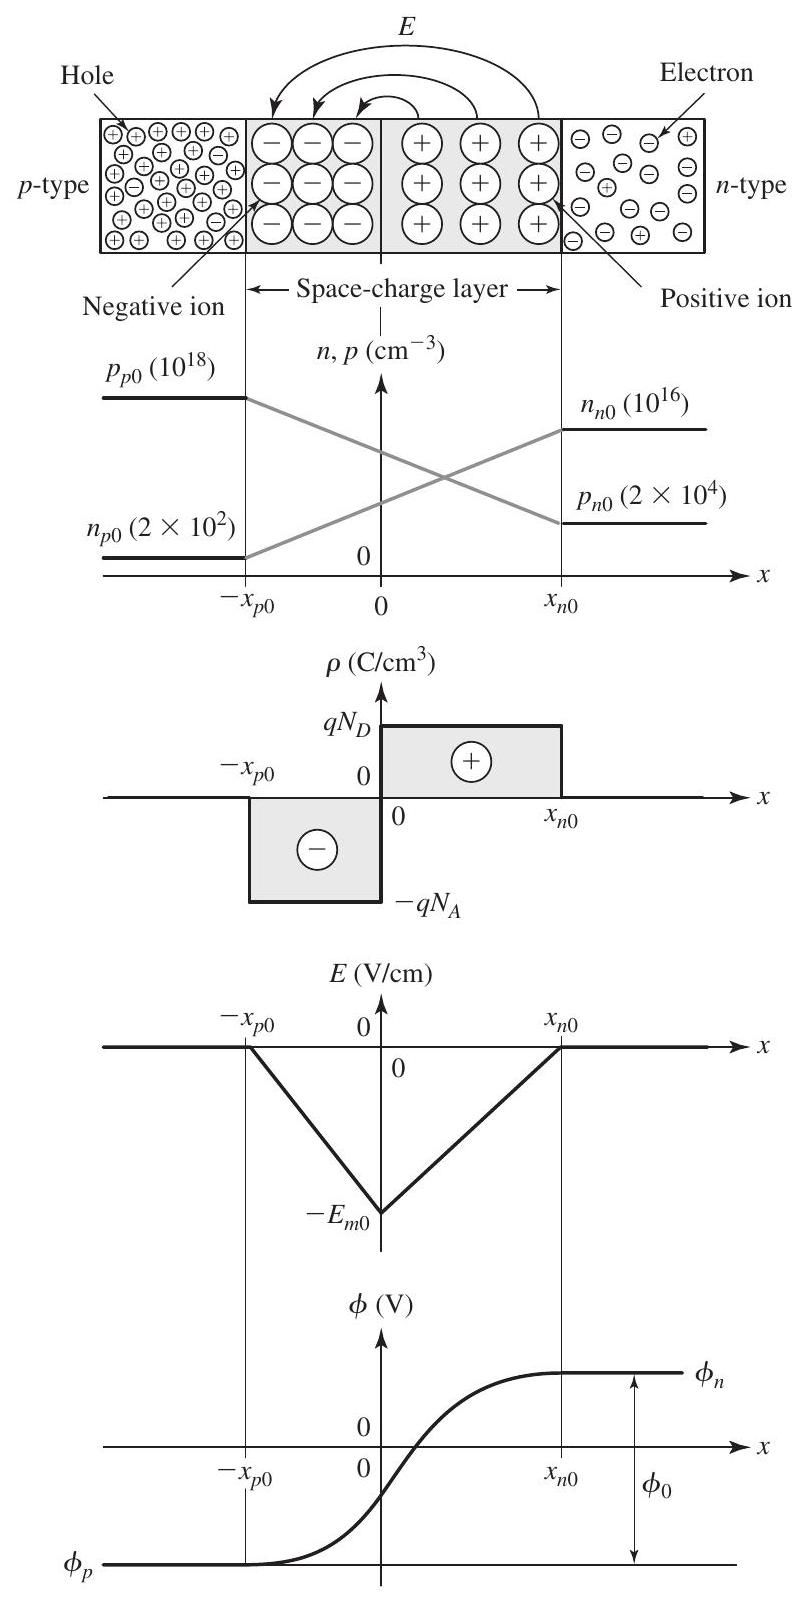
\includegraphics[max width=\textwidth, center]{2024_10_31_0c26dbfd3a789ec9acb1g-050}

FIGURE 1.39 Equilibrium conditions in a pn slab.\\
due to their diffusion across the junction. The SCL, in turn, establishes an electric field $E$ in the direction opposing diffusion. As holes and electrons keep diffusing, the SCL keeps building up, until an equilibrium condition is reached whereby the electric field $E$ will exactly counterbalance the tendency of holes and electrons to diffuse further. Thereafter, the net current across the junction will be zero.

\section*{Equilibrium Conditions}
We express the equilibrium conditions by writing $J_{p(\text { drifif })}+J_{p(\text { diff }}=0$ and $J_{n(\text { drift })}+$ $J_{n(d i f f)}=0$. Taking the origin of the $x$-axis at the point of contact between the $p$ and $n$ regions, also called the metallurgical junction, we have, by Eqs. (1.25) through (1.27),


\begin{align*}
& q p(x) \mu_{p} E(x)-q D \frac{d p(x)}{d x}=0  \tag{1.31a}\\
& q n(x) \mu_{n} E(x)+q D_{n} \frac{d n(x)}{d x}=0 \tag{1.31b}
\end{align*}


where we are emphasizing that $p, n$, and $E$ are now functions of the position $x$ along the $p n$ slab.

The equilibrium situation is illustrated further in Fig. 1.39, where the origin of the $x$ axis has been taken right at the metallurgical junction. The edges of the SCL are located at $-x_{p 0}$ and $+x_{n 0}$, respectively. The charge density $\rho$ (in $\mathrm{C} / \mathrm{cm}^{3}$ ) due to immobile ions is $+q N_{D}$ in the $n$ side of the SCL, and $-q N_{A}$ in the $p$ side. Denoting the cross-sectional area of the $p$ and $n$ slabs as $A$, we find the total SCL charge in the $n$-side as $Q^{+}=q N_{D} \times A x_{n 0}$, and the total SCL charge in the $p$-side as $Q^{-}=-q N_{A} \times A x_{p 0}$. Charge neutrality requires that $Q^{+}=-Q^{-}$, or $q N_{D} A x_{n 0}=q N_{A} A x_{p 0}$. Simplifying, we get


\begin{equation*}
\frac{x_{p 0}}{x_{n 0}}=\frac{N_{D}}{N_{A}} \tag{1.32}
\end{equation*}


indicating that in an asymmetrically doped $p n$ junction such as ours $\left(N_{A} \gg N_{D}\right)$, the SCL will extend mostly into the more lightly doped side $\left(x_{n 0} \gg x_{p 0}\right)$. This makes sense as it takes more volume in the lightly doped side to come up with the same number of ions as the heavily doped side. We have tried to convey this pictorially in Fig. 1.39, top.

We readily visualize the electric field strength $E$ as a function of $x$ by counting the field lines. Each line starts on a positive ion at the right and ends on a negative ion at the left. The number of lines is maximum at the metallurgical junction $(x=0)$ and decreases linearly as we move away on either side, to finally drop to zero at the edges of the SCL. The regions outside the SCL, where the electric field is zero, are aptly called the neutral regions. Because of asymmetric doping, the profile of $E$ is a scalene triangle, and a negative one as $E$ is in the direction of negative $x$.

We readily find a relationship between the maximum strength $E_{m 0}$ and the SCL edges $x_{p 0}$ and $x_{n 0}$ via Gauss's theorem. In a one-dimensional case such as this, this theorem is expressed as


\begin{equation*}
\frac{d E}{d x}=\frac{\rho(x)}{\varepsilon_{s i}} \tag{1.33}
\end{equation*}


where $\varepsilon_{s i}$ is silicon's permittivity $\left(\varepsilon_{s i}=1.04 \mathrm{pF} / \mathrm{cm}\right)$. In the right portion of the SCL we have $d E / d x=E_{m 0} / x_{n}$ and $\rho / \varepsilon_{s i}=q N_{D} / \varepsilon_{s i}$, so $E_{m 0} / x_{n 0}=q N_{D} / \varepsilon_{s i t}$. Applying similar considerations to the left side of the SCL and solving for $E_{m 0}$ gives


\begin{equation*}
E_{m 0}=\frac{q N_{A} x_{p 0}}{\varepsilon_{s i}}=\frac{q N_{D} x_{n 0}}{\varepsilon_{s i}} \tag{1.34}
\end{equation*}


\section*{The Built-in Potential $\boldsymbol{\phi}_{\mathbf{0}}$}
From basic electrostatics we know that an electric field is always accompanied by an electric potential gradient. For a one-dimensional situation such as ours, the relationship between field $E$ and potential $\phi$ is, by Eq. (1.24), $E=-d \phi / d x$. Rewriting as $\phi=-\int E d x$, we visualize $\phi$ as the negative of the area enclosed by the $E$ curve. Since $E$ has a linear profile, $\phi$ will have a quadratic profile, as shown in Fig. 1.39, bottom. We observe that outside the SCL the profile of $\phi$ is flat because $E=0$ there. The potentials there are denoted as $\phi_{p}$ and $\phi_{n}$, respectively. We now wish to find expressions for $\phi_{p}$ and $\phi_{n}$, as well as for the built-in equilibrium potential $\phi_{0}$, defined as

$$
\phi_{0}=\phi_{n}-\phi_{p}
$$

This potential acts as a barrier preventing holes and electrons from diffusing further, and is the result of the charge redistribution taking place automatically at either side of the metallurgical junction when we create it. Solving for $E(x)$ in Eq. (1.31) and using Einstein's relations of Eq. (1.28) gives

$$
E(x) d x=V_{T} \frac{d p(x)}{p(x)}=-V_{T} \frac{d n(x)}{n(x)}
$$

Using again $\phi(x)=-\int E(x) d x$ and integrating from $-x_{p 0}$ to $+x_{n 0}$ gives

$$
\int_{\phi_{p}}^{\phi_{n}} d \phi(x)=-V_{T} \int_{p_{p 0}}^{p_{n 0}} \frac{d p(x)}{p(x)}=V_{T} \int_{n_{n 0}}^{n_{n 0}} \frac{d n(x)}{n(x)}
$$

where the integration limits are, respectively, the values of $\phi, p$, and $n$ at $x=-x_{p 0}$ and $x=+x_{n 0}$. This gives


\begin{equation*}
\phi_{0}=\phi_{n}-\phi_{p}=V_{T} \ln \frac{p_{p 0}}{p_{n 0}}=V_{T} \ln \frac{n_{n 0}}{n_{p 0}} \tag{1.35}
\end{equation*}


Using Eq. (1.10), we can also write


\begin{gather*}
\phi_{0}=V_{T} \ln \frac{N_{A} N_{D}}{n_{i}^{2}}  \tag{1.36a}\\
\phi_{n}=V_{T} \ln \frac{N_{D}}{n_{i}}  \tag{1.36b}\\
\phi_{p}=V_{T} \ln \frac{n_{i}}{N_{A}} \tag{1.36c}
\end{gather*}


Note that since in practical junctions $N_{A}$ and $N_{D}$ are greater than $n_{i}$, we have $\phi_{n}>0$ and $\phi_{p}<0$. Moreover, since $N_{A}$ and $N_{D}$ appear in the argument of the logarithmic function, the $\phi \mathrm{s}$ of Eq. (1.36) are not that sensitive to variations in the doping doses.\\
(a) Find the room-temperature values of $\phi_{n}, \phi_{p}$, and $\phi_{0}$ for a junction with the

EXAMPLE 1.6 dopings of Eq. (1.29).\\
(b) Find $\phi_{0}$ if both doping doses are increased by an order of magnitude.

\section*{Solution}
(a) We have $\phi_{n}=(26 \mathrm{mV}) \ln \left[10^{16} /\left(1.4 \times 10^{10}\right)\right]=0.350 \mathrm{~V}, \phi_{p}=-0.470 \mathrm{~V}$, and $\phi_{0}=0.350-(-0.470)=0.820 \mathrm{~V}$.\\
(b) Now $\phi_{0}=0.940 \mathrm{~V}$, not much of a change because of the logarithmic dependence. It pays to think of $\phi_{0}$ as being close to 1 V , regardless of the particular doping values.

\section*{The Electric Field $E_{m 0}$, the SCL Width $X_{d 0}$, and the SCL Charge $\boldsymbol{Q}_{j 0}$}
We now wish to derive an expression for all other pertinent junction parameters in equilibrium. The maximum field strength $E_{m 0}$ is found once again via $\int d \phi(x)=-\int E(x) d x$, where we integrate from $-x_{p 0}$ to $x_{n 0}$. The left-hand side integrates simply to $\phi_{0}$, while the right-hand side represents the negative of the area of the electric-field triangle. Consequently, we have


\begin{equation*}
\phi_{0}=\frac{\left(x_{p 0}+x_{n 0}\right) E_{m 0}}{2} \tag{1.37}
\end{equation*}


But, according to Eq. (1.34),


\begin{equation*}
x_{p 0}=\frac{\varepsilon_{s i}}{q N_{A}} E_{m 0} \quad x_{n 0}=\frac{\varepsilon_{s i}}{q N_{D}} E_{m 0} \tag{1.38}
\end{equation*}


Substituting $x_{p 0}$ and $x_{n 0}$ into Eq. (1.37), expressing $\phi_{0}$ via Eq. (1.36a), and solving for $E_{m 0}$, we finally get


\begin{equation*}
E_{m 0}=\sqrt{\frac{2 q \phi_{0}}{\varepsilon_{s i}} \frac{N_{A} N_{D}}{N_{A}+N_{D}}} \tag{1.39}
\end{equation*}


If we insert Eq. (1.39) back into Eq. (1.38), we obtain the equilibrium edges of the SCL as


\begin{equation*}
x_{p 0}=\sqrt{\frac{2 \varepsilon_{s i} \phi_{0}}{q N_{A}} \frac{N_{D}}{N_{A}+N_{D}}} \quad x_{n 0}=\sqrt{\frac{2 \varepsilon_{s i} \phi_{0}}{q N_{D}} \frac{N_{A}}{N_{A}+N_{D}}} \tag{1.40}
\end{equation*}


The sum of the two is aptly called the equilibrium $S C L$ width, $X_{d 0}=x_{p 0}+x_{n 0}$. By Eq. (1.40),


\begin{equation*}
X_{d 0}=\sqrt{\frac{2 \varepsilon_{s i} \phi_{0}}{q}\left(\frac{1}{N_{A}}+\frac{1}{N_{D}}\right)} \tag{1.41}
\end{equation*}


The equilibrium junction charge is $Q_{j 0}=Q^{+}=q N_{D} A x_{n 0}$, where $A$ is the aforementioned junction's cross-sectional area. Using Eq. (1.40),


\begin{equation*}
Q_{j 0}=A \sqrt{2 \varepsilon_{s i} q \phi_{0} \frac{N_{A} N_{D}}{N_{A}+N_{D}}} \tag{1.42}
\end{equation*}


Assuming a cross-sectional area $A=(100 \mu \mathrm{~m}) \times(100 \mu \mathrm{~m})$ for a $p n$ junction with the doping doses of Eq. (1.29), find $E_{m 0}, X_{d 0}, x_{p 0}, x_{n 0}$, and $Q_{j 0}$.

\section*{Solution}
From Example $1.6, \phi_{0}=0.820 \mathrm{~V}$. Also, since in our case $N_{A} \gg N_{D}$, we can approximate $N_{A} N_{D} /\left(N_{A}+N_{D}\right) \cong N_{D}=10^{16} \mathrm{~cm}^{-3}$. Then, Eq. (1.39) gives

$$
E_{m 0} \cong \sqrt{\frac{2 \times 1.602 \times 10^{-19} \times 0.820 \times 10^{16}}{1.04 \times 10^{-12}}}=5.03 \times 10^{4} \mathrm{~V} / \mathrm{cm}
$$

and Eq. (1.41) gives

$$
X_{d 0} \cong \sqrt{\frac{2 \times 1.04 \times 10^{-12} \times 0.820}{1.602 \times 10^{-19}}\left(\frac{1}{10^{16}}\right)}=3.26 \times 10^{-5} \mathrm{~cm}=0.326 \mu \mathrm{~m}
$$

Similarly, Eq. (1.40) gives $x_{p 0}=0.003 \mu \mathrm{~m}$ and $x_{n 0}=0.323 \mu \mathrm{~m}$, confirming that the SCL extends almost entirely into the more lightly doped side, which in our example is the $n$ side. Finally, since the junction area is $A=\left(100 \times 10^{-4} \mathrm{~cm}\right)^{2}=$ $10^{-4} \mathrm{~cm}^{2}$, Eq. (1.42) gives $Q_{j 0}=5.23 \mathrm{pC}$.

\section*{Exercise 1.5}
Show that


\begin{equation*}
\phi(0)=\phi_{p}+\frac{N_{D}}{N_{A}+N_{D}} \phi_{0} \tag{1.43}
\end{equation*}


Hence, verify that $\phi(0)=0$ only in the case of symmetrically doped junctions $\left(N_{D}=N_{A}\right)$. Otherwise, $\phi(0)>0$ for $N_{D}>N_{A}$, and $\phi(0)<0$ for $N_{D}<N_{A}$ (as in the case of Fig. 1.39).

\subsection*{1.6 EFFECT OF EXTERNAL BIAS ON THE SCL PARAMETERS}
Let us now investigate the effect of applying a voltage $v$ across our $p n$ junction in the manner of Fig. 1.40, top. (Note that the polarity convention for $v$ is positive at the $p$ side and negative at the $n$ side; for $v>0$ the $p n$ junction is said to be forward biased, and for $v<0$ it is reverse biased.) By KVL, the potential barrier across the spacecharge layer (SCL) becomes $\phi_{0}-v$. With a changed profile for $\phi$, the electric field strength $E$ will also have to change. Since the field lines making up $E$ come from the uncovered ions of the SCL, the SCL's width $X_{d}=x_{n}+x_{p}$ will have to change accordingly. Specifically, we can state that:

\begin{itemize}
  \item Forward biasing the junction $(v>0)$ lowers the potential barrier as well as the electric field compared to the unbiased case, and thus shrinks $X_{d}$.
  \item Conversely, reverse biasing the junction $(v<0)$ raises the potential barrier and the electric field, and thus widens $X_{d}$. For a visual comparison, Fig. 1.40 uses gray lines to show the unbiased situation.\\
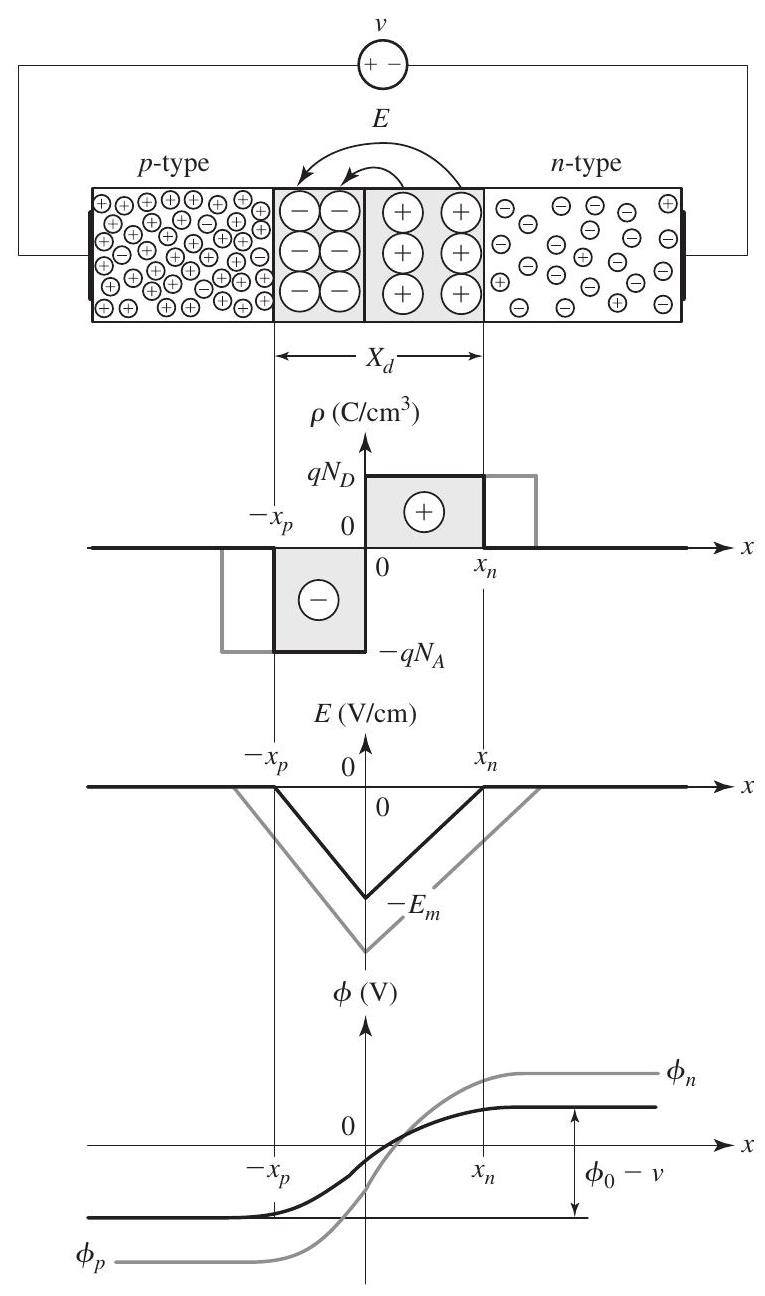
\includegraphics[max width=\textwidth, center]{2024_10_31_0c26dbfd3a789ec9acb1g-055}
\end{itemize}

FIGURE 1.40 Effect of forward-biasing a pn junction.\\
To investigate the effect of the external bias $v$ quantitatively, we simply replace $\phi_{0}$ with $\left(\phi_{0}-v\right)$ in Eqs. (1.39) through (1.42). Thus, rewriting Eq. (1.39) with $E_{m}(v)$ in place of $E_{m 0}$ and $\left(\phi_{0}-v\right)$ in place of $\phi_{0}$, we get the maximum electric-field strength as a function of $v$

$$
E_{m}(v)=\sqrt{\frac{2 q\left(\phi_{0}-v\right)}{\varepsilon_{s i}} \frac{N_{A} N_{D}}{N_{A}+N_{D}}}=\sqrt{\frac{2 q \phi_{0}}{\varepsilon_{s i}} \frac{N_{A} N_{D}}{N_{A}+N_{D}}} \sqrt{1-\frac{v}{\phi_{0}}}
$$

This is expressed more concisely as


\begin{equation*}
E_{m}(v)=E_{m 0} \sqrt{1-\frac{v}{\phi_{0}}} \tag{1.44}
\end{equation*}


\begin{center}
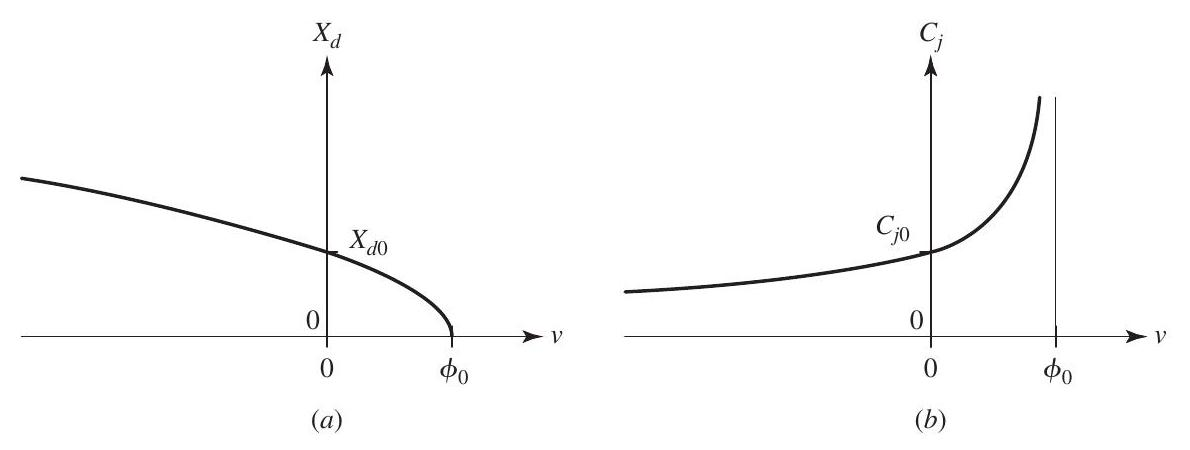
\includegraphics[max width=\textwidth]{2024_10_31_0c26dbfd3a789ec9acb1g-056}
\end{center}

FIGURE 1.41 Voltage dependence of the (a) SCL width and (b) junction capacitance for $m=1 / 2$.\\
where $E_{m 0}$, aptly called the zero-bias $(v=0)$ value of $E_{m}$, was derived in Eq. (1.39). Proceeding in similar manner for the SCL's width, we find


\begin{equation*}
X_{d}(v)=X_{d 0} \sqrt{1-\frac{v}{\phi_{0}}} \tag{1.45}
\end{equation*}


where $X_{d 0}$ is the zero-bias $(v=0)$ value of $X_{d}$, which was derived in Eq. (1.41). The voltage dependence of $X_{d}$ is depicted in Fig. 1.41a. Finally, the junction charge is


\begin{equation*}
Q_{j}(v)=Q_{j 0} \sqrt{1-\frac{v}{\phi_{0}}} \tag{1.46}
\end{equation*}


where $Q_{j 0}$ is the zero-bias $(v=0)$ value of $Q_{j}$ as given in Eq. (1.42).

\section*{The Junction Capacitance $\boldsymbol{C}_{\boldsymbol{j}}$}
Since applying a voltage across a pn junction redistributes its SCL charge, the junction exhibits capacitive behavior. The junction capacitance is $C_{j}=d Q_{j} / d v$. Differentiating Eq. (1.46) and rearranging,


\begin{equation*}
C_{j}(v)=\frac{C_{j 0}}{\left(1-v / \phi_{0}\right)^{m}} \tag{1.47a}
\end{equation*}


where


\begin{equation*}
C_{j 0}=A \sqrt{\frac{\varepsilon_{s i} q}{2 \phi_{0}} \frac{N_{A} N_{D}}{N_{A}+N_{D}}} \tag{1.47b}
\end{equation*}


is the zero-bias $(v=0)$ value of $C_{j}$ and $m$, called the grading coefficient, is $1 / 2$ in the present case, which assumes an abrupt junction. Practical junctions often have a graded doping profile, in which case it can be shown ${ }^{2}$ that a more appropriate value is $m=1 / 3$. The actual value of $m$ can be found experimentally by measuring $C_{j}$ for different values of $v$ and then using data-interpolation to indirectly find $m$. The voltage dependence of $C_{j}$ is depicted in Fig. 1.41b.\\
\includegraphics[max width=\textwidth, center]{2024_10_31_0c26dbfd3a789ec9acb1g-057}

FIGURE 1.42 (a) The junction capacitance $C_{j}$, and $(b)$ its parallel-plate equivalent.\\
Combining Eqs. (1.41), (1.45), and (1.47) with $m=1 / 2$, we put $C_{J}$ in yet another insightful form


\begin{equation*}
C_{j}(v)=\varepsilon_{s i} \frac{A}{X_{d}(v)} \tag{1.48}
\end{equation*}


This is the same form as that of a parallel-plate capacitor consisting of two plates of area $A$ separated by a dielectric material having permittivity $\varepsilon_{s i}$ and thickness $X_{d}$. This equivalence is illustrated in Fig. 1.42. However, unlike a fixed capacitor, the present one exhibits a voltage-dependent plate separation $X_{d}(v)$, indicating nonlinear capacitance behavior, as already seen in Fig. 1.41b. We also observe that Eq. (1.47a) predicts $C_{j} \rightarrow \infty$ for $v \rightarrow \phi_{0}$. This, of course, cannot happen in practice, indicating that Eq. $(1.47 a)$, whose derivation is based on a number of simplifying assumptions, no longer holds as $v$ approaches $\phi_{0}$.

EXAMPLE 1.8 Find $C_{j 0}$ for the junction of Example 1.7. Then, assuming $m=1 / 2$, calculate $E_{m}, X_{d}$, $Q_{j}$, and $C_{j}$ for $(a) v=+0.65 \mathrm{~V}$, and $(b) v=-5 \mathrm{~V}$.

\section*{Solution}
(a) Using Eq. (1.47b) we readily find $C_{j 0}=3.19 \mathrm{pF}$. Moreover

$$
\sqrt{1-v / \phi_{0}}=\sqrt{1-0.65 / 0.82}=0.455
$$

indicating a decrease in $E_{m}, X_{d}$, and $Q_{j}$, but an increase in $C_{j}$. Indeed, at $v=+0.65 \mathrm{~V}$ we have $E_{m}=5.03 \times 10^{4} \times 0.455=2.29 \times 10^{4} \mathrm{~V} / \mathrm{cm}$, $X_{d}=0.148 \mu \mathrm{~m}, Q_{j}=2.38 \mathrm{pC}$, and $C_{j}=3.19 / 0.455=7.01 \mathrm{pF}$.\\
(b) Now $E_{m}, X_{d}$, and $Q_{j}$ will increase but $C_{j}$ will decrease by $\sqrt{1-(-5) / 0.82}=$ 2.66, so $E_{m}=13.4 \times 10^{4} \mathrm{~V} / \mathrm{cm}, X_{d}=0.869 \mu \mathrm{~m}, Q_{j}=13.9 \mathrm{pC}$, and $C_{j}=1.20 \mathrm{pF}$.

Remark: It pays to keep in mind the following orders of magnitude for low-power junctions:

$$
\phi_{0} \sim 1 \mathrm{~V} \quad E_{m} \sim 10^{4} \mathrm{~V} / \mathrm{cm} \quad X_{d} \sim 1 \mu \mathrm{~m} \quad Q_{j} \sim 1 \mathrm{pC} \quad C_{j} \sim 1 \mathrm{pF}
$$

\subsection*{1.7 THE pn DIODE EQUATION}
Forward-biasing a pn junction affects not only the parameters of its space-charge layer (SCL), but also the concentration profiles of its charge carriers in the neutral regions, and quite dramatically so, as we are about to see. The starting point is offered by Eq. (1.35), which we turn around by taking the logarithms throughout and solving for the minority concentrations,


\begin{align*}
& p_{n 0}=p_{p 0} e^{-\phi_{0} / V_{T}}  \tag{1.49a}\\
& n_{p 0}=n_{n 0} e^{-\phi_{0} / V_{T}} \tag{1.49b}
\end{align*}


These equations relate the hole and the electron concentrations at either side of the SCL for the unbiased $(v=0)$ equilibrium situation. If we now forward bias the junction $(v>0), E$ will decrease and thus allow holes to diffuse from the $p$ side, through the SCL, to the $n$ side, and electrons from the $n$ to the $p$ side. We can still use Eq. (1.49) to relate the concentrations right at the edges of the SCL, also called boundary concentrations, provided we replace $\phi_{0}$ with $\phi_{0}-v$. The result is


\begin{align*}
& p_{n}\left(x_{n}\right)=p_{p}\left(-x_{p}\right) e^{-\left(\phi_{0}-v\right) / V_{T}}  \tag{1.50a}\\
& n_{p}\left(-x_{p}\right)=n_{n}\left(x_{n}\right) e^{-\left(\phi_{0}-v\right) / V_{T}} \tag{1.50b}
\end{align*}


The so-called low-level injection assumption stipulates that even after biasing, the minority concentrations at either side of the SCL continue to remain much lower than the majority concentrations there, and thus leave the latter essentially undisturbed compared to the unbiased case. This means that we can let $p_{p}\left(-x_{p}\right)=p_{p 0}$ and $n_{n}\left(x_{n}\right)=$ $n_{n 0}$ in Eq. (1.50). Reusing Eq. (1.49), we can then write


\begin{gather*}
p_{n}\left(x_{n}\right)=p_{n 0} e^{v / V_{T}}  \tag{1.51a}\\
n_{p}\left(-x_{p}\right)=n_{p 0} e^{v / V_{T}} \tag{1.51b}
\end{gather*}


Referred to as the law of the junction, Eq. (1.51) relates the boundary values of the minority concentrations to the applied voltage $v$. Though the derivations were made for the forward-bias case $(v>0)$, this law holds also for the reverse-bias case $(v<0)$.

Assuming the doping doses of Eq. (1.29), find the minority and majority concentrations at either edge of the SCL if the junction is forward biased with $v=0.65 \mathrm{~V}$. Comment on your results.

\section*{Solution}
By Eq. (1.30), $p_{p}\left(-x_{p}\right)=p_{p 0} \cong 10^{18} / \mathrm{cm}^{3}$ and $n_{n}\left(x_{n}\right) \cong n_{n 0} \cong 10^{16} / \mathrm{cm}^{3}$. Moreover, $n_{p 0} \cong 2 \times 10^{2} / \mathrm{cm}^{3}$, and $p_{n 0} \cong 2 \times 10^{4} / \mathrm{cm}^{3}$. Since $\exp (0.650 / 0.026) \cong 7.2 \times 10^{10}$, Eq. (1.51) gives

$$
\begin{aligned}
& p_{n}\left(x_{n}\right) \cong 2 \times 10^{4} \times 7.2 \times 10^{10}=1.44 \times 10^{15} / \mathrm{cm}^{3} \\
& n_{p}\left(-x_{p}\right) \cong 2 \times 10^{2} \times 7.2 \times 10^{10}=1.44 \times 10^{13} / \mathrm{cm}^{3}
\end{aligned}
$$

\begin{center}
\includegraphics[max width=\textwidth]{2024_10_31_0c26dbfd3a789ec9acb1g-059}
\end{center}

FIGURE 1.43 Forward biasing a pn junction creates an excess of minority charges in the neutral regions. These charges diffuse away from the SCL, giving raise to diffusion currents.

These boundary values are shown numerically in Fig. 1.43. We observe that a forward bias of only 0.65 V causes $p_{n}\left(x_{n}\right)$ to shoot up from $2 \times 10^{4} / \mathrm{cm}^{3}$ to $1.44 \times 10^{15} / \mathrm{cm}^{3}$ ! However, this is still less than the majority concentration there $\left(10^{16} / \mathrm{cm}^{3}\right)$, thus confirming low-level injection. Likewise, $n_{p}\left(-x_{p}\right)$ has jumped from $2 \times 10^{2} / \mathrm{cm}^{3}$ to $1.44 \times 10^{13} / \mathrm{cm}^{3}$. This too is quite a number, yet it is much less than the majority concentration there $\left(10^{18} / \mathrm{cm}^{3}\right)$, again indicating low-level injection.

\section*{Excess Minority Concentrations}
It is apparent that forward biasing the $p n$ junction establishes an excess of minority carriers at both edges of the SCL. The excess concentrations are $p_{n}^{\prime}\left(x_{n}\right)=p_{n}\left(x_{n}\right)-p_{n 0}$ at the right edge, and $n_{p}^{\prime}\left(-x_{p}\right)=n_{p}\left(-x_{p}\right)-n_{p 0}$ at the left edge. By Eq. (1.51), these excesses can be expressed as


\begin{gather*}
p_{n}^{\prime}\left(x_{n}\right)=p_{n 0}\left(e^{v / V_{T}}-1\right)  \tag{1.52a}\\
n_{p}^{\prime}\left(-x_{p}\right)=n_{p 0}\left(e^{v / V_{T}}-1\right) \tag{1.52b}
\end{gather*}


Once minority excesses have been established, the carriers will diffuse away from the SCL toward regions of lower excess concentrations (holes from $x_{n}$ toward the right, electrons from $-x_{p}$ toward the left). In both cases, their diffusion takes place in a sea of oppositely-charged majority carriers, indicating a high chance of recombination. In fact, the further away we go from the SCL's edges, the less and less excess minority carriers we are likely to find.

This diffuse-and-recombine process is governed by the diffusion equation, which for excess holes takes on the form ${ }^{2}$

$$
D_{p} \frac{d^{2} p_{n}^{\prime}(x)}{d x^{2}}=\frac{p_{n}^{\prime}(x)}{\tau_{p}}
$$

where $\tau_{p}$ is the mean recombination time, also called the mean lifetime of the excess holes. A similar equation holds for excess electrons, but with $\tau_{n}$ as the mean recombination time. The solution to the diffusion equation is an exponential decay with $x$ for holes, and with $-x$ for electrons, in the manner illustrated in Fig. 1.43, middle. Mathematically, the decay for holes is expressed as


\begin{equation*}
p_{n}^{\prime}(x)=p_{n 0}\left(e^{v / V_{T}}-1\right) e^{-\left(x-x_{n}\right) / L_{p}} \tag{1.53}
\end{equation*}


where the quantity


\begin{equation*}
L_{p}=\sqrt{D_{p} \tau_{p}} \tag{1.54a}
\end{equation*}


is called the hole diffusion length, in cm . It represents the distance from $x_{n}$ at which $p_{n}^{\prime}(x)$ drops to $1 / e(36.8 \%)$ of its boundary value $p_{n}^{\prime}\left(x_{n}\right)$. A similar expression holds for excess electrons in the $p$ side, but with the electron diffusion length


\begin{equation*}
L_{n}=\sqrt{D_{n} \tau_{n}} \tag{1.54b}
\end{equation*}


The lengths $L_{p}$ and $L_{n}$ are typically on the order of $10^{1} \mu \mathrm{~m}$, so we generally have $L_{p} \gg x_{n}$ and $L_{n} \gg x_{p}$.

Note that $p_{n}^{\prime} \rightarrow 0$ at the right end of the $n$-type slab $\left(x=W_{n}\right)$, as the excess holes undergo total recombination with the electrons of the metal electrode there. Likewise, $n_{p}^{\prime} \rightarrow 0$ at the left end of the $p$-type slab $\left(x=-W_{p}\right)$, as excess electrons undergo total removal by the metal electrode there.

By Eq. (1.27a) the diffusion of excess holes toward the right results in the current density $J_{p}(x)=-q D_{p} d p_{n}^{\prime}(x) / d x$. Differentiating Eq. (1.53) and substituting gives


\begin{equation*}
J_{p}(x)=q D_{p} \frac{p_{n 0}}{L_{p}}\left(e^{v / V_{T}}-1\right) e^{-\left(x-x_{n}\right) / L_{p}} \tag{1.55a}
\end{equation*}


A similar expression holds for the current density due to excess electrons diffusing toward the left, except that we need to replace $x$ with $-x$ in the exponent,


\begin{equation*}
J_{n}(x)=q D_{n} \frac{n_{p 0}}{L_{n}}\left(e^{v / V_{T}}-1\right) e^{\left(x+x_{p}\right) / L_{n}} \tag{1.55b}
\end{equation*}


We expect recombination within the (thin) depletion region to be negligible, so $J_{p}$ and $J_{n}$ will essentially be constant there. With reference to Fig. 1.43, bottom, we find the total current density within the SCL as $J_{\text {tot }}=J_{p}\left(x_{n}\right)+J_{n}\left(-x_{p}\right)$. Using Eq. (1.55), we readily get


\begin{equation*}
J_{\text {tot }}=q\left(\frac{D_{p} p_{n 0}}{L_{p}}+\frac{D_{n} n_{p 0}}{L_{n}}\right)\left(e^{v / V_{T}}-1\right) \tag{1.56}
\end{equation*}


Note that Fig. 1.43, bottom, shows only the minority diffusion currents. For a complete picture of conduction we need to show also the majority diffusion currents. Owing to the charge conservation principle, $J_{\text {tot }}$ must be constant throughout the slab. We can thus obtain each majority current component by taking the graphical difference between the total current and the corresponding minority current component, or $J_{p}=J_{\text {tot }}-J_{n}$ to the left of $-x_{p}$, and $J_{n}=J_{\text {tot }}-J_{p}$ to the right of $x_{n}$. The result, shown in Fig. 1.44, shows how fascinating conduction is inside a pn slab.\\
\includegraphics[max width=\textwidth, center]{2024_10_31_0c26dbfd3a789ec9acb1g-061}

FIGURE 1.44 Minority and majority current densities inside a pn slab.

If we were to scan the slab from left to right, our description of conduction would be as follows

\begin{itemize}
  \item At the far left we see a current of mainly holes diffusing toward the right on their way to recombine with electrons. Some of these holes disappear by recombination in the $p$ side itself, others manage to make it all the way to the SCL, from where they emerge as minority carriers in the $n$ side. As they progress toward the right, they are further annihilated by electrons.
  \item Moving closer to the SCL while still on the $p$ side, we note that $J_{p}$ has subsided somewhat, but at the expense of an increase in $J_{n}$, so as to ensure the constancy of $J_{\text {tor }}$. The fact that close to the SCL, $J_{p}$ has subsided doesn't necessarily imply a reduction in hole concentration there. In fact, Example 1.9 has revealed that at $x=-x_{p}$ there are $10^{18}$ holes $/ \mathrm{cm}^{3}$ pressing against the SCL, quite a number compared to the $1.44 \times 10^{13}$ electrons/cm ${ }^{3}$ available there. Out of these $10^{18} \mathrm{holes} /$ $\mathrm{cm}^{3}$, only $1.44 \times 10^{15}$ holes $/ \mathrm{cm}^{3}$ manage to emerge from the SCL, at the right.
  \item Moving now inside the SCL, we see a two-way traffic of holes and electrons, hardly recombining with each other because $X_{d}$ is much shorter than the diffusion lengths $L_{p}$ and $L_{n}$. Because of asymmetric doping as well as differences in the hole and electron diffusivities and diffusion lengths, $J_{p}$ and $J_{n}$ are generally different inside the SCL.
  \item As we move past the SCL into the $n$ region, we note that excess holes fade away, annihilated by the majority of electrons present there. We instead observe a progressively larger current of electrons moving toward the left, on their way either to annihilate holes while still in the $n$ side, or to be annihilated by holes once they cross the SCL to emerge in the $p$ side.
\end{itemize}

\section*{The Diode Equation}
The overall current $i$ through a $p n$ junction of cross-sectional area $A$ is readily found as $i=A J_{\text {tot }}$. Using Eqs. (1.56), along with Eq. (1.30), we get what is commonly referred to as the diode equation


\begin{equation*}
i=I_{s}\left(e^{v / V_{T}}-1\right) \tag{1.57}
\end{equation*}


where $I_{s}$ is a scaling factor called the saturation current,


\begin{equation*}
I_{s}=A \times n_{i}^{2}(T) \times q\left(\frac{D_{p}}{L_{p} N_{D}}+\frac{D_{n}}{L_{n} N_{A}}\right) \tag{1.58}
\end{equation*}


This factor gives an indication of how much current $i$ we get for a given applied voltage $v$. For low-power junctions, $I_{s}$ is typically on the order of femto-amperes ( $1 \mathrm{fA}=$ $10^{-15} \mathrm{~A}$ ). We observe that $I_{s}$ depends on:

\begin{itemize}
  \item The cross-sectional area $A$ (the larger $A$, the higher the current-just as with ordinary resistors)
  \item Temperature $T$, especially via $n_{i}^{2}(T)$
  \item The doping densities $N_{A}$ and $N_{D}$, the diffusivities $D_{p}$ and $D_{n}$, and the diffusion lengths $L_{p}$ and $L_{n}$.
\end{itemize}

As we proceed we shall find that most practical junctions are fabricated with one side much more heavily doped than the other. When this is the case, one of the terms within parentheses in Eq. (1.58) becomes negligible, and $I_{s}$ is determined primarily by the term with the smaller doping concentration in its denominator. In our working $p n$ junction example, for which $N_{A} \gg N_{D}$, the dominant term in Eq. (1.58) is the first one, stemming from the injection of holes into the more lightly doped $n$-side. As we know, this is also the side into which most of the SCL extends. For obvious reasons, asymmetrically-doped junctions are also referred to as one-sided junctions. An example will better illustrate.\\
(a) Estimate $i$ if the $p n$ junction of Example 1.7 is biased at $v=0.65 \mathrm{~V}$. Assume $D_{p}=10 \mathrm{~cm}^{2} / \mathrm{s}, L_{p}=5 \mu \mathrm{~m}, D_{n}=7 \mathrm{~cm}^{2} / \mathrm{s}$, and $L_{n}=10 \mu \mathrm{~m}$. Comment on your results.\\
(b) Find the area $A$ needed for the junction of part (a) to give $i=0.15 \mathrm{~mA}$ at $v=0.65 \mathrm{~V}$.

\section*{Solution}
(a) Inserting the given data into Eq. (1.58) gives

$$
\begin{aligned}
I_{s} & =10^{-4} \times 2 \times 10^{20} \times 1.602 \times 10^{-19}\left(\frac{10}{5 \times 10^{-4} \times 10^{16}}+\frac{7}{10 \times 10^{-4} \times 10^{18}}\right) \\
& =6.41+0.02=6.43 \mathrm{fA}
\end{aligned}
$$

As expected of a one-sided junction such as the present one, $I_{s}$ is determined primarily by one term, namely, the first term, representing hole injection. Electron injection into the heavily-doped $p$-side has little say in this case. Finally, we use Eq. (1.57) to find

$$
i=6.43 \times 10^{-15}\left(e^{650 / 26}-1\right)=463 \mu \mathrm{~A}
$$

(b) To lower $i$ from 0.463 mA to 0.15 mA , we need to lower $A$ in proportion, that is, from $10^{-4} \mathrm{~cm}^{2}$ to $(0.15 / 0.463) \times 10^{-4} \mathrm{~cm}^{2}$, or to $0.324 \times 10^{-4} \mathrm{~cm}^{2}$. This requires a square area of about $(57 \mu \mathrm{~m}) \times(57 \mu \mathrm{~m})$.

\section*{Short-Base Diodes}
In the diode example of Fig. 1.43 the neutral regions are long enough to provide sufficient distance for the minority charges to recombine with the majority charges as they diffuse away from the SCL. Aptly called a long-base diode, this structure occurs when the device is fabricated with dimensions $W_{n} \gg L_{p}$ and $W_{p} \gg L_{n}$. As we progress, we shall see that $p n$ diodes are also fabricated with $W_{n} \ll L_{p}$, or $W_{p} \ll L_{n}$, or both. A popular example is the base-emitter junction of a bipolar junction transistor, this being the reason why such a structure is referred to as a short-base diode.

With $W_{n} \ll L_{p}$, the holes injected into the $n$-side don't have much of a chance to recombine while diffusing toward the right, indicating that $J_{p}$ will essentially be\\
\includegraphics[max width=\textwidth, center]{2024_10_31_0c26dbfd3a789ec9acb1g-064}

FIGURE 1.45 Minority carrier concentrations in a forward-biased short-base diode fabricated with $W_{n} \ll L_{p}$ and $W_{p} \ll L_{n}$.\\
constant in the $n$-side. By Eq. $(1.27 a)$, this implies, in turn, a constant slope for $p_{n}(x)$, as depicted in Fig. 1.45. If the condition $W_{p} \ll L_{n}$ holds, similar considerations apply to $J_{n}$ and $n_{p}(x)$ in the $p$-side. To find the $i-v$ characteristic of a short-base diode, we start with $J_{p}=-q D_{p} d p_{n}^{\prime}(x) / d x$, where $p_{n}^{\prime}(x)$ is the excess hole density in the $n$-side. The slope of the triangle in Fig. 1.45 is readily found as

$$
\frac{d p_{n}^{\prime}(x)}{d x}=-\frac{p_{n}\left(x_{n}\right)-p_{n 0}}{W_{n}-x_{n}} \cong-\frac{p_{n 0}\left(e^{v / V_{T}}-1\right)}{W_{n}}
$$

where we have exploited the fact that usually $x_{n} \ll W_{n}$. Similar considerations hold for the $p$-side slope $d n_{p}^{\prime}(x) / d x$. Proceeding as in the derivation of Eq. (1.58), we readily find that a short-base diode still obeys Eq. (1.57), but with the following expression for the saturation current,


\begin{equation*}
I_{s} \cong A n_{i}^{2} q\left(\frac{D_{p}}{W_{n} N_{D}}+\frac{D_{n}}{W_{p} N_{A}}\right) \tag{1.59}
\end{equation*}


This is identical to that of Eq. (1.58), except for the replacements $L_{p} \rightarrow W_{n}$ and $L_{p} \rightarrow W_{n}$. Considering that in a short-base diode the $W \mathrm{~s}$ are much smaller than the $L \mathrm{~s}$, it is apparent that this structure requires a smaller cross-sectional area $A$ to achieve the same value of $I_{s}$. Another advantage is that the amount of excess charge stored in a forward-biased short-base diode is much smaller than that of a long-base device operating at the same current. This results in much faster switching times, as we shall see in Chapter 6.

EXAMPLE 1.11 Repeat Example 1.10, but for the case in which the diode has been fabricated with $W_{p}=0.5 \mu \mathrm{~m}$ and $W_{n}=1 \mu \mathrm{~m}$. Compare and comment.

\section*{Solution}
Since we have a one-sided junction with $N_{A} \gg N_{D}$, we expect the first term within parentheses in Eq. (1.59) to dominate, just like its counterpart of Eq. (1.58). Considering that the value of $W_{n}$ given here is five times as small as the value of $L_{p}$ given in Example 1.10, we anticipate a fivefold increase in $I_{s}$, or $I_{s} \cong 6.41 \times 5 \cong$ 33 fA . With the same applied voltage $v$, the current $i$ will also increase fivefold,

$$
i \cong 33 \times 10^{-15} e^{650 / 26} \cong 2.4 \mathrm{~mA}
$$

To lower $i$ from 2.4 mA to 0.15 mA , we need to lower $A$ in proportion, from $10^{-4} \mathrm{~cm}^{2}$ to $(0.15 / 2.4) \times 10^{-4} \mathrm{~cm}^{2}$, or to $0.063 \times 10^{-4} \mathrm{~cm}^{2}$. This can be achieved with a square area of $(25 \mu \mathrm{~m}) \times(25 \mu \mathrm{~m})$.

\subsection*{1.8 THE REVERSE-BIASED pn JUNCTION}
Reverse biasing a pn junction further increases the existing potential barrier, thus inhibiting hole and electron diffusion across the metallurgical junction. Given this strong preference to conduct in the forward direction, the $p n$ junction exhibits diode behavior, so from now on we shall use the words pn junction and diode interchangeably.

For sufficiently negative values of the applied voltage $v$ (say, for $v<-4 V_{T} \cong-0.1 \mathrm{~V}$ ), Eq. (1.57) predicts that $i$ will saturate at $-I_{s}$ (hence, the name saturation current). As we know, for low-power diodes, $I_{s}$ is typically in the fA range. However, the actual reverse current found in a pn junction, which we shall denote as $I_{R}$, is orders of magnitude higher than $I_{s}$, typically in the pA to nA range. This stems from the thermal generation of holeelectron pairs within the space-charge layer SCL, which we ignored in the course of our analysis. In fact, even though we have been referring to the SCL as the depletion region, thermal generation of hole-electron pairs does continue to take place there, and once generated, holes and electrons are swept in opposite directions by the strong local electric field $E$, resulting in a combined drift current from the $n$ side, through the SCL, to the $p$ side. Intuitively we expect $I_{R}$ to be proportional to the SCL's volume $A X_{d}$, and since $X_{d}$ increases with the amount of reverse bias, as per Eq. (1.45), $I_{R}$ will also increase with the reverse voltage in square-root fashion. Depending on the quality of fabrication, leakage current may also flow across the surface of the pn junction, further contributing to $I_{R}$.

The overall reverse current $I_{R}$ is a strong function of temperature, a behavior that engineers remember via the following important rule of thumb:

The reverse current $I_{R}$ of a pn junction doubles for about every $10^{\circ} \mathrm{C}$ of temperature increase

Once we know $I_{R}$ at some reference temperature $T_{0}$, we can estimate it at any other temperature $T$ using


\begin{equation*}
I_{R}(T) \cong I_{R}\left(T_{0}\right) \times 2^{\left(T-T_{0}\right) / 10} \tag{1.60}
\end{equation*}


If at $25^{\circ} \mathrm{C}$ a certain diode exhibits $I_{R}=1 \mathrm{pA}$, estimate $I_{R}(a)$ at $125{ }^{\circ} \mathrm{C}$, and (b) at $-25^{\circ} \mathrm{C}$.

\section*{Solution}
(a) By Eq. (1.60), $I_{R}\left(125^{\circ} \mathrm{C}\right) \cong 10^{-12} \times 2^{(125-25) / 10} \cong 1 \mathrm{nA}$. (b) Likewise, $I_{R}\left(-25^{\circ} \mathrm{C}\right)$ $\cong 0.03 \mathrm{pA}$.

\section*{Reverse Breakdown}
If we gradually increase the reverse bias of a $p n$ junction, a voltage is reached, called the breakdown voltage ( $B V$ ), at which the reverse current shoots up in magnitude from the negligible value $I_{R}$ discussed above to much higher values. The name stems from the fact that the $i-v$ curve bends sharply, or breaks down. This does not necessarily imply a destructive process-in fact, one always limits the reverse current within safety levels by interposing a suitable resistor in series between the driving voltage source and the reverse-biased junction. Figure 1.46 shows the complete $i-v$ characteristic of a typical $p n$ junction.

The breaking down of the $i-v$ curve evidently indicates the sudden availability of huge quantities of mobile charges to produce the much increased current levels. This sudden availability is the result of either of two separate mechanisms: Zener\\
\includegraphics[max width=\textwidth, center]{2024_10_31_0c26dbfd3a789ec9acb1g-066}

FIGURE 1.46 The complete $i-v$ characteristic of a pn junction.\\
breakdown, and avalanche breakdown. The former occurs in heavily doped junctions, the latter in lightly doped junctions.

\begin{itemize}
  \item In heavily doped junctions the electric field within the SCL is already fairly strong, and increasing it further with several volts of reverse bias will give it enough strength to strip electrons away from the covalent bonds and thus create electron-hole pairs. The field itself then sweeps these newly freed charges out of the SCL (holes into the $p$ side, electrons into the $n$ side), thus sustaining much higher currents than in the case of thermal generation alone. Called Zener effect, this phenomenon occurs for BV values on the order of 6 V or less.
  \item In lightly doped junctions the electric field is not strong enough to break covalent bonds directly. However, with the wider SCL widths now available, the field has more space to accelerate any free electrons that happen to be within the SCL. Given sufficient kinetic energy, these electrons will free new electron-hole pairs as they collide with the atoms of the crystal lattice. These secondary electrons can in turn free additional electrons, in an effect aptly called avalanche effect. This effect occurs for BV values on the order of 6 V or higher. In the neighborhood of 6 V the Zener and avalanche effects may coexist.
\end{itemize}

When designed to operate deliberately in the breakdown region, a diode is commonly referred to as a Zener diode, regardless of whether the actual breakdown mechanism is of the Zener or avalanche type. The coordinates of an operating point $Q_{B}$ in the breakdown region are conveniently relabeled as $-I_{Z}$ and $-V_{Z}$, respectively. The slope of the diode curve in the breakdown region is denoted as $1 / r_{z}$, and sufficiently to the left of the breakdown knee it is approximately constant. Depending on fabrication details, $r_{z}$ is on the order of $10^{1}$ to $10^{3} \Omega$.

The temperature coefficient at a given breakdown-region operating point $Q_{B}\left(I_{Z}, V_{Z}\right)$ is defined as

$$
\operatorname{TC}\left(V_{Z}\right)=\left.\frac{\partial V_{Z}}{\partial T}\right|_{I_{Z}}
$$

We again distinguish two cases:

\begin{itemize}
  \item In the case of the Zener effect, increasing temperature will increase thermal agitation and thus facilitate covalent breakdown, so we need to turn down the applied voltage $V_{Z}$ a bit if we want to maintain the same current level $I_{Z}$ at a higher temperature. Thus, $\mathrm{TC}\left(V_{Z}\right)<0$ in the Zener case.
  \item In the avalanche case, thermal agitation will increase the frequency of collisions of free electrons with atoms of the crystal lattice, making it more difficult for electrons to accelerate and acquire sufficient kinetic energy to trigger the avalanche mechanism. Now we need to turn $u p$ the applied voltage $V_{Z}$ a bit if we want to maintain the same current level $I_{Z}$, so $\mathrm{TC}\left(V_{Z}\right)>0$ in the avalanche case. We summarize the two mechanisms as follows:
\end{itemize}

The Zener effect occurs in heavily doped junctions, $V_{Z}$ is lower than about 6 V , and $\mathrm{TC}\left(V_{Z}\right)<0$

The avalanche effect occurs in lightly doped junctions, $V_{Z}$ is higher than about 6 V , and $\mathrm{TC}\left(V_{Z}\right)>0$

By playing with the impurity concentrations during processing, the manufacturer can control the BV of a junction to a particular value. Two familiar representatives are the base-emitter (BE) and the base-collector (BC) junctions forming the bipolar junction transistor (BJT). The BE junction is heavily doped, and thus breaks down by the Zener effect in the neighborhood of 6 V . This low BV value poses no problem when the BJT is operated in the forward-active (FA) region, where the BE junction is forward biased. However, in the FA region the BC junction is reverse biased. To prevent it from going into breakdown, the collector region is doped lightly, indicating that BC breakdown is of avalanche type.

\subsection*{1.9 FORWARD-BIASED DIODE CHARACTERISTICS}
For sufficiently high forward voltages (in practice, for $v>4 V_{T} \cong 0.1 \mathrm{~V}$ ), we can ignore unity in Eq. (1.57), and write


\begin{equation*}
i_{D}=I_{S} e^{v_{D} / V_{T}} \tag{1.61}
\end{equation*}


where we are now using subscript $D$ to signify operation well into the forward region. This equation represents a perfectly exponential $i-v$ characteristic. Also called the ideal diode equation, it is satisfied by practical pn junctions quite well over a wide range of currents, typically on the order of six decades, making it one of the most predictable laws of electronics. The exponential law enjoys some fascinating properties, as we are about to see.

Equation (1.61) is readily turned around as


\begin{equation*}
v_{D}=V_{T} \ln \left(\frac{i_{D}}{I_{s}}\right) \tag{1.62}
\end{equation*}


In this form, it allows us to find the voltage drop $v_{D}$ needed to sustain a given current $i_{D}$.

\section*{Properties of the Exponential Characteristic}
The slope of the diode curve at a given operating current $I_{D}$ in the forward-bias region is defined as $g_{d}=d i_{D} /\left.d v_{D}\right|_{I_{D}}$, and is called the dynamic conductance of the diode. Differentiating Eq. (1.61), we get


\begin{equation*}
g_{d}=\frac{I_{D}}{V_{T}} \tag{1.63}
\end{equation*}


indicating that slope is linearly proportional to the operating current $I_{D}$. The reciprocal of $g_{d}$ is called the dynamic resistance of the diode, or $r_{d}=1 / g_{d}=V_{T} / I_{D}$. Both $g_{d}$ and $r_{d}$ span quite a range of values, depending on the operating current. Note the following significant values:

$$
r_{d}(1 \mathrm{~mA})=26 \Omega \quad r_{d}(1 \mu \mathrm{~A})=26 \mathrm{k} \Omega \quad r_{d}(1 \mathrm{nA})=26 \mathrm{M} \Omega
$$

The parameters $r_{d}$ and $g_{d}$ form the basis of small-signal diode circuit analysis, to be studied later.

Given a diode carrying a certain current $I_{D}$, we wish to find the voltage change $\Delta V_{D}$ required to change its current from $I_{D}$ to $m I_{D}$, where $m$ is some multiplicative factor. Using Eq. (1.62), we find such a voltage change as $\Delta V_{D}=V_{T} \ln \left(m I_{D} / I_{s}\right)-$ $V_{T} \ln \left(I_{D} / I_{s}\right)=V_{T} \ln \left[\left(m I_{D} / I_{s}\right) /\left(I_{D} / I_{s}\right)\right]$, or

$$
\Delta V_{D}=V_{T} \ln m
$$

Two popular cases are a change in current by an octave ( $m=2^{ \pm 1}$ ), or by a decade $\left(m=10^{ \pm 1}\right)$, which give, respectively, $\Delta V_{D(\text { oct })}=(26 \mathrm{mV}) \times( \pm \ln 2) \cong \pm 18 \mathrm{mV}$, and $\Delta V_{D(\mathrm{dec})}=(26 \mathrm{mV}) \times( \pm \ln 10) \cong \pm 60 \mathrm{mV}$. These findings form the basis of the following important rules of thumb, illustrated pictorially in Fig. 1.47a:

To effect an octave change in $I_{D}$ we need to change $V_{D}$ by 18 mV

To effect a decade change in $I_{D}$ we need to change $V_{D}$ by 60 mV\\
A convenient feature of the above rules is that they are independent of the particular quiescent point $Q_{F}$ on the diode curve where the changes are made. For instance, consider a diode initially operating at a quiescent current of $10 \mu \mathrm{~A}$. If we wish to double its current to $20 \mu \mathrm{~A}$, we need an increase $\Delta V_{D}=18 \mathrm{mV}$. To effect the tenfold change $10 \mu \mathrm{~A} \rightarrow 100 \mu \mathrm{~A}$ we need an increase $\Delta V_{D}=60 \mathrm{mV}$. Likewise, the change $10 \mu \mathrm{~A} \rightarrow 1 \mu \mathrm{~A}$ requires a decrease $\Delta V_{D}=-60 \mathrm{mV}$. If you wish to change $I_{D}$ from\\
\includegraphics[max width=\textwidth, center]{2024_10_31_0c26dbfd3a789ec9acb1g-069}

FIGURE 1.47 Illustrating some important rules of thumb for pn junctions.\\
$10 \mu \mathrm{~A}$ to $50 \mu \mathrm{~A}$, pretend first to raise it from $10 \mu \mathrm{~A}$ to $100 \mu \mathrm{~A}\left(\Delta V_{D}=+60 \mathrm{mV}\right)$, and then to lower it from $100 \mu \mathrm{~A}$ to $50 \mu \mathrm{~A}\left(\Delta V_{D}=-18 \mathrm{mV}\right)$, for a net change $V_{D}=60-18=42 \mathrm{mV}$.

\section*{Temperature Dependence}
Whether we use Eq. (1.61) or (1.62), it is apparent that the diode characteristic depends on temperature via $V_{T}$ as well as $I_{s}$. A convenient way to characterize the overall thermal dependence is via the temperature coefficient of the forward voltage drop at a given operating current $I_{D}$, defined as


\begin{equation*}
\mathrm{TC}\left(V_{D}\right)=\left.\frac{\partial V_{D}}{\partial T}\right|_{I_{D}} \tag{1.64}
\end{equation*}


Differentiating Eq. (1.62), we obtain


\begin{equation*}
\mathrm{TC}\left(V_{D}\right)=\left.\frac{\partial\left[V_{T} \ln \left(I_{D} / I_{s}\right)\right]}{\partial T}\right|_{I_{D}}=\frac{V_{D}}{T}-V_{T}\left(\frac{d I_{s} / d T}{I_{s}}\right) \tag{1.65}
\end{equation*}


According to Eqs. (1.58) and (1.59), $I_{s} \propto n_{i}^{2}(T) D(T)$, where $n_{i}$ is the intrinsic concentration and $D$ is the diffusivity, both of which are functions of temperature $T$. By Eq. (1.21), $n_{i}^{2}(T) \propto T^{3} e^{-V_{01} / V_{T}}$, where $V_{G 0}=1.205 \mathrm{~V}$ is the bandgap voltage for silicon. By Eqs. (1.20) and (1.28), $D(T)=(k T / q) \mu(T)$, where $\mu(T)$ is the mobility, in turn a function of temperature of the type $\mu(T) \propto T^{m}, m \cong-1.5$. Combining all this we have

$$
\begin{gathered}
I_{s} \propto T^{4+m} e^{-V_{c o}(q / k T)} \\
\frac{d I_{s} / d T}{I_{s}}=\frac{(4+m) T^{4+m-1} e^{-V_{\sigma_{0}}(q / k T)}+T^{4+m} e^{-V_{c o l}(q / k T)} \times V_{G 0}\left(q / k T^{2}\right)}{T^{4+m} e^{-V_{c 0}(q / k T)}}=\frac{4+m}{T}+\frac{V_{G 0}}{T V_{T}}
\end{gathered}
$$

Substituting into Eq. (1.65) and simplifying, we finally get


\begin{equation*}
\operatorname{TC}\left(V_{D}\right)=\frac{V_{D}-(4+m) V_{T}-V_{G 0}}{T} \tag{1.66}
\end{equation*}


Assuming $V_{D}=0.65 \mathrm{~V}$ at $T=300 \mathrm{~K}$, Eq. (1.66) gives $\mathrm{TC}\left(V_{D}\right) \cong-2.1 \mathrm{mV} /{ }^{\circ} \mathrm{C}$. Engineers remember $p n$ junction thermal behavior via the following rule of thumb, pictorially illustrated in Fig. 1.47b:

At room-temperature the forward voltage-drop of a pn diode drifts by about $-2 \mathrm{mV} /{ }^{\circ} \mathrm{C}$

Once we know $V_{D}$ at some reference temperature $T_{0}$, we can estimate it at any other temperature $T$ using


\begin{equation*}
V_{D}(T) \cong V_{D}\left(T_{0}\right)-(2 \mathrm{mV}) \times\left(T-T_{0}\right) \tag{1.67}
\end{equation*}


EXAMPLE 1.13 If at $25^{\circ} \mathrm{C}$ a certain diode exhibits $V_{D}=650 \mathrm{mV}$ at $I_{D}=0.1 \mathrm{~mA}$, estimate $V_{D}$ at:\\
(a) $T=70^{\circ} \mathrm{C}$ and $I_{D}=0.1 \mathrm{~mA}$.\\
(b) $T=0^{\circ} \mathrm{C}$ and $I_{D}=0.1 \mathrm{~mA}$.\\
(c) $T=50^{\circ} \mathrm{C}$ and $I_{D}=0.02 \mathrm{~mA}$.\\
(d) $T=40^{\circ} \mathrm{C}$ and $I_{D}=4 \mathrm{~mA}$.

\section*{Solution}
Using the rules of thumb learned thus far we get:\\
(a) $V_{D} \cong 650-2 \times(70-25)=650-90=560 \mathrm{mV}$.\\
(b) $V_{D} \cong 650-2 \times(0-25)=650+50=700 \mathrm{mV}$.\\
(c) First, pretend to lower $I_{D}=$ from 0.1 mA to $0.01 \mathrm{~mA}\left(\Delta V_{D}=-60 \mathrm{mV}\right)$, and then double it ( $\Delta V_{D}=+18 \mathrm{mV}$ ) to end up at 0.02 mA with the net value $V_{D} \cong 650-60+18=608 \mathrm{mV}$. Finally, pretend to increase temperature from $25^{\circ} \mathrm{C}$ to $50^{\circ} \mathrm{C}$, for an additional change $\Delta V_{D}=-2 \times(50-25)=-50 \mathrm{mV}$. The final value is thus $V_{D} \cong 608-50=558 \mathrm{mV}$.\\
(d) Proceeding as in part ( $c$ ) we find $V_{D}=650+60+18+18-2 \times(40-25)=$ 716 mV .

If a forward-biased diode is placed in series with a reverse-biased Zener diode of the opposite temperature coefficient, or $\mathrm{TC}\left(V_{Z}\right)=-\mathrm{TC}\left(V_{D}\right) \cong+2 \mathrm{mV}$, the thermal variations of the two devices will cancel each other out to yield a composite voltage drop $V_{R E F}=V_{Z}+V_{D}$ approaching zero temperature coefficient. This technique is used in the implementation of thermally stable voltage references. The best stability is achieved for $V_{Z} \cong 6.2 \mathrm{~V}$, thus yielding $V_{R E F} \cong 6.2+0.7=6.9 \mathrm{~V}$ with $\mathrm{TC}\left(V_{R E F}\right) \rightarrow 0$.

\section*{Deviations from Ideality}
Rewriting Eq. (1.62) as $v_{D}=V_{T}\left(\ln i_{D}-\ln I_{s}\right)$, or

$$
\ln i_{D}=\left(\frac{1}{V_{T}}\right) v_{D}+\ln I_{s}
$$

indicates that if we plot $i_{D}$ versus $v_{D}$ on semi-logarithmic paper ( $v_{D}$ on the linear axis, $i_{D}$ on the logarithmic axis), we get a curve of the type

$$
y=\left(1 / V_{T}\right) x+y(0)
$$

This is a straight line with slope $\left(1 / V_{T}\right)$ and $0-\mathrm{V}$ intercept at $i_{D}=I_{S}$. This feature proves very convenient in the characterization of a diode. Given a set of measured data, we can easily find the best-fit straight line; then, we find its slope to obtain the experimental value of $V_{T}$, and we extrapolate the line in the limit $v_{D} \rightarrow 0$ to find its intercept on the $i_{D}$ axis and thus obtain the experimental value of $I_{s}$.

The semi-log-plot of an actual low-power pn diode characteristic is more likely to appear as in Fig. 1.48. The curve is fairly straight over a wide range of currents, typically from 1 nA to 1 mA , but deviates from ideality both at the high and\\
\includegraphics[max width=\textwidth, center]{2024_10_31_0c26dbfd3a789ec9acb1g-072}

FIGURE 1.48 Illustrating the effect of the emission coefficient $n$ at low and at high current levels.\\
low ends of the range. These deviations stem from various approximations that were made in the course of the derivations leading to the ideal diode equation. Specifically, deviations at the high end of the current range are caused by the presence of bulk resistance in the neutral regions as well as high-level injection effects, while deviation at the low end is caused by loss of mobile charges to recombination within the space-charge layer (SCL). We now wish to examine these approximations in greater detail.

\begin{itemize}
  \item In our derivations we have assumed zero electric field inside the regions at either side of the SCL, so that the voltage that we apply across the terminals is transmitted entirely to the edges of the SCL itself. However, like any conductor, each of these regions exhibits a nonzero-if small—ohmic resistance called the bulk resistance. Denoting the overall resistance (sum of the $p$-side and $n$-side bulk resistances) as $r_{s}$, we observe that in response to the externally applied voltage $v_{D}$, the actual voltage $v_{J}$ reaching the junction is, by KVL,
\end{itemize}


\begin{equation*}
v_{J}=v_{D}-r_{S} i_{D} \tag{1.68}
\end{equation*}


When the diode is operated at low current levels, the voltage drop across the bulk material is negligible and $v_{J} \cong v_{D}$. Not so at the upper end of the current range, where this drop may become significant and cause a deviation of the actual $i-v$ characteristic from exponential ideality. On semi-log paper, this appears as a curvature for values of $i_{D}$ on the order of 1 mA or higher.

\begin{itemize}
  \item If the applied voltage across the junction is increased to the point of making the minority densities at the SCL edges comparable to the majority densities there, the low-level injection assumption no longer holds, and the diode equation now takes on the form
\end{itemize}


\begin{equation*}
i_{D}=I_{s} e^{v_{D} / n V_{T}} \tag{1.69a}
\end{equation*}


where $n$, called the emission coefficient (not to be confused with the electron concentration $n!$ ) is such that $n \rightarrow 1$ under low-level injection conditions, but $n \rightarrow 2$ when these conditions no longer hold. The inverse equation is now


\begin{equation*}
v_{D}=n V_{T} \ln \left(\frac{i_{D}}{I_{s}}\right) \tag{1.69b}
\end{equation*}


Rewriting as

$$
\ln i_{D}=\left(\frac{1}{n V_{T}}\right) v_{D}+\ln I_{s}
$$

indicates that the slope of the semi-log curve is now $1 /\left(n V_{T}\right)$. Clearly, for $n=2$ the slope is only half of that for $n=1$. We can find the experimental value of the quantity $n V_{T}$ through a mere slope measurement on the semi-log plot.

\begin{itemize}
  \item Equation (1.69) with $n \rightarrow 2$ holds also at the low end of the current range, but for a completely different reason, namely the loss of mobile charges to recombination (trapping) within the SCL. Evidently, our assumption of constant current densities within the SCL is not exactly valid. It must be said that loss to recombination occurs regardless of the operating point on the $i-v$ curve, but its effect is noticeable only at the low-end, where the forward current is comparable to, or even smaller than that due to loss. On semi-log paper, this appears as a curvature for values of $i_{D}$ on the order of 1 pA or lower.
\end{itemize}

EXAMPLE 1.14 If a $p n$ junction with $I_{s}=1 \mathrm{fA}$ gives $I_{D}=1 \mathrm{~mA}$ at $V_{D}=725 \mathrm{mV}$, find $r_{S}$.

\section*{Solution}
By Eq. (1.62) the actual junction voltage is $V_{J}=(26 \mathrm{mV}) \ln \left(10^{-3} / 10^{-15}\right)=718.4 \mathrm{mV}$. By Eq. (1.68), $r_{S}=(725-718.4) / 1=6.6 \Omega$.

\subsection*{1.10 Dc ANALYSIS OF pn DIODE CIRCUITS}
A task that arises all the time in the analysis of diode circuits is finding a diode's quiescent point $Q=Q\left(I_{D}, V_{D}\right)$. As we know, if the diode is embedded in an otherwise linear circuit, this task simplifies considerably if we replace the surrounding circuitry with its Thévenin equivalent and thus end up with the situation of Fig. 1.49a. Here, $V_{O C}$ is the open-circuit voltage that the external circuit would produce between the nodes corresponding to the anode and the cathode, but with the diode removed, and $R_{e q}$ is the external circuit's equivalent resistance, that is, the resistance as seen by the diode.

\section*{Load-Line Analysis}
The operating point can be visualized graphically as the intercept of the diode curve and the load line, as already seen in Fig. $1.5 b$ for the case of the ideal diode. The situation is depicted in Fig. $1.49 b$ for the case of a forward-biased pn junction diode. Though graphical analysis helps us develop a visual feel for a circuit's workings, we usually need to find the operating point $Q$ numerically, the issue that we are going to address next.\\
\includegraphics[max width=\textwidth, center]{2024_10_31_0c26dbfd3a789ec9acb1g-074}

FIGURE 1.49 Finding the quiescent point $Q$ of a $p n$-junction diode embedded in a linear circuit.

\section*{Iterative Analysis}
With reference to Fig. 1.49a we observe that the diode current is, by Ohm's law,


\begin{equation*}
I_{D}=\frac{V_{O C}-V_{D}}{R_{e q}} \tag{1.70}
\end{equation*}


Also, the diode voltage is, by Eq. (1.69b),


\begin{equation*}
V_{D}=n V_{T} \ln \frac{I_{D}}{I_{s}} \tag{1.71}
\end{equation*}


where $n$ is the emission coefficient, $1 \leq n \leq 2$. In the following we shall assume $n=1$ for simplicity, but the ensuing analysis can readily be generalized to the case $n \neq 1$ by replacing $V_{T}$ with $n V_{T}$. Substituting Eq. (1.70) into (1.71) gives


\begin{equation*}
V_{D}=n V_{T} \ln \frac{V_{O C}-V_{D}}{R_{e q} I_{s}} \tag{1.72}
\end{equation*}


This is a transcendental equation in that it does not provide us with a closed-form expression for the unknown $V_{D}$. However, we can solve it by iterations. To this end, we start out with a reasonable initial estimate for $V_{D}$, we insert it in the right-hand side of Eq. (1.72) to come up with a better estimate, and then we insert this new estimate back in the right-hand side to come up with yet a better estimate, repeating the procedure if necessary, until the result settles within a predetermined resolution.

In the circuit of Fig. 1.49a let $R_{e q}=1 \mathrm{k} \Omega$, and let the diode have $n=1, V_{T}=26 \mathrm{mV}$, and $I_{s}=1 \mathrm{fA}$. Estimate $V_{D}$ down to the mV , as well as $I_{D}$, if (a) $V_{O C}=1.5 \mathrm{~V}$, (b) $V_{O C}=3 \mathrm{~V}$, and (c) $V_{O C}=0.75 \mathrm{~V}$.

\section*{Solution}
(a) In the various $p n$-junction examples encountered so far we have found that $V_{D}$ is typically in the range of $0.6-0.7 \mathrm{~V}$, so let us arbitrarily start out with the initial guess $\mathrm{V}_{D(0)}=0.65 \mathrm{~V}$. Plugging into Eq. (1.72) gives the new estimate

$$
V_{D(1)}=n V_{T} \ln \frac{V_{O C}-V_{D(0)}}{R_{e q} I_{s}}=0.026 \ln \frac{1.5-0.65}{10^{3} \times 10^{-15}}=0.714 \mathrm{~V}
$$

Using this new value as initial guess we find

$$
V_{D(2)}=n V_{T} \ln \frac{V_{O C}-V_{D(1)}}{R_{e q} I_{s}}=0.026 \ln \frac{1.5-0.714}{10^{-12}}=0.712 \mathrm{~V}
$$

Iterating once more we find

$$
V_{D(3)}=n V_{T} \ln \frac{V_{O C}-V_{D(2)}}{R_{e q} I_{s}}=0.026 \ln \frac{1.5-0.712}{10^{-12}}=0.712 \mathrm{~V}
$$

Since the result hasn't changed within the intended resolution of 0.001 V ( $=1 \mathrm{mV}$ ), we conclude that $V_{D}=712 \mathrm{mV}$. Finally, the current is, by Eq. (1.70),

$$
I_{D}=\frac{1.5-0.712}{10^{3}}=0.788 \mathrm{~mA}
$$

(b) This time let us start out with the initial guess $V_{D(0)}=0.7 \mathrm{~V}$. Then,

$$
V_{D(1)}=0.026 \ln \frac{3-0.7}{10^{-12}}=0.740 \mathrm{~V}
$$

One more iteration confirms that this is actually the desired value, or $V_{D}=$ 740 mV within a 1-mV resolution. Then, $I_{D}=(3-0.74) / 1=2.26 \mathrm{~mA}$.\\
(c) Starting again with $V_{D(0)}=0.65 \mathrm{~V}$, we find

$$
V_{D(1)}=0.026 \ln \frac{0.75-0.65}{10^{-12}}=0.659 \mathrm{~V}
$$

Three more iterations confirm the final value $V_{D}=657 \mathrm{mV}$. Consequently, $I_{D}$ $=(0.75-0.657) / 1=93 \mu \mathrm{~A}$.

Remark 1: In going from (a) to (b) we have doubled $V_{O C}$, and in going from (a) to (c) we have halved $V_{O C}$; however, $I_{D}$ has neither doubled nor halved, as the presence of the diode renders the circuit nonlinear.

Remark 2: We could have found $I_{D}$ also using the diode equation. For instance, in part (a) we could have calculated

$$
I_{D}=I_{S} e^{V_{D} / n V_{T}}=10^{-15} e^{712 / 26}=0.782 \mathrm{~mA}
$$

This disagrees with the value of 0.788 mA found via Eq. (1.70). True, both calculations are afflicted by roundoff errors, but even so, which result is the more dependable of the two? Here's an important point to keep in mind: because of the high sensitivity of the exponential function to even small variations in its exponent, the value of $V_{D}$ in the exponent must be known very accurately for the result to be also accurate. By contrast, the value of the $V_{D}$ in the linear Eq. (1.70) need not be as accurate, and yet it will still yield a dependable $I_{D}$ value. Consequently, 0.788 mA is the more accurate value in our example.

Remark 3: Of course, if we use the exponential form with a more accurate value of $V_{D}$ the resulting $I_{D}$ will also be more accurate. In fact, using just one more significant digit from the third-iteration result, which is $V_{D(3)}=0.7122 \mathrm{~V}$ (rather than the truncated value of 0.712 V ) we get

$$
I_{D}=10^{-15} e^{712.2 / 26}=0.788 \mathrm{~mA}
$$

This matches that found via Eq. (1.70). If, for some reason, you need to use the diode equation in its exponential form, make sure that you know the value of $V_{D}$ to an adequate degree of accuracy!

\section*{Piecewise-Linear Approximation and Large-Signal Diode Models}
Load-line analysis provides a graphical means for visualizing a diode's role in a circuit, and iterative analysis provides a numerical means for calculating a diode's operating point. In practice, whether we analyze an existing diode circuit or we design a new one, we need faster, if only approximate, analysis techniques. Moreover, as we apply these techniques, we wish to draw from the wealth of knowledge acquired in prerequisite linear-circuits courses. Both requirements are met by effecting upon the actual pn-junction characteristic of Fig. 1.46 a piecewise-linear approximation as depicted in Fig. 1.50. Specifically, the actual curve, shown in shaded form, is approximated with three straight segments, each corresponding to a different region of operation, namely, the forward (ON), the cutoff (CO), and the breakdown (BD) regions. We make the following observations:

\begin{itemize}
  \item When a pn junction is forward biased, its characteristic is exponential, that is, a curve that after a brief knee, shoots up quite rapidly, no matter which current range we choose to display. The curves of Figs. 1.47 and $1.49 b$ were doctored a bit to allow for a better visualization of the details under discussion, but the actual curve is indeed as in Fig. 1.46-quite steep. We know from one of the rules of thumb that increasing $V_{D}$ by a mere 60 mV raises $I_{D}$ tenfold, while decreasing it by 60 mV lowers $I_{D}$ tenfold, indicating that within the\\
\includegraphics[max width=\textwidth, center]{2024_10_31_0c26dbfd3a789ec9acb1g-076}
\end{itemize}

FIGURE 1.50 Piecewise-linear approximations and large signal models of the pn junction diode in its three regions of operation: forward (ON), cutoff (CO), and breakdown (BD).\\
range $V_{D} \pm 60 \mathrm{mV}, I_{D}$ undergoes a 100-to-1 change! For practical purpose, when a junction conducts only $1 / 100$ of its normal current, it can be regarded as being cut off (in digital applications, even a 10-to-1 ratio will do). Considering that a low-power silicon junction operating in the mA range typically exhibits a roomtemperature voltage drop of about 0.7 V , we approximate the exponential curve with a vertical segment located at $v=V_{D(\text { on })}=0.7 \mathrm{~V}$. The corresponding diode model is thus a battery of value $V_{D(\text { on })}$, as shown. For obvious reasons, this model is referred to as a constant voltage-drop model. The reader, who may find this approximation unconvincing, will soon realize that it is actually quite effective in providing us with a quick feel for the workings of diode circuits. During a second and more detailed pass, one can always use iterative techniques or computer simulation such as PSpice to refine the analysis and come up with more accurate results.

\begin{itemize}
  \item From the knee leading to the exponential rise to the knee leading to the breakdown drop, the current is negligibly small, indicating that for practical purposes we can regard the junction as cut off (CO). The corresponding diode model is an open circuit, as shown. Note that the cutoff region extends to the right of the origin, all the way to the onset of the exponential raise. Even though for $v>0$ the junction is, strictly speaking, forward biased, the actual current between 0 V and the knee leading to the exponential raise is simply too small for the junction to be considered convincingly on. So, we take a weakly forward-biased junction as being effectively cut off.
  \item Well into the breakdown (BD) region, the characteristic is close to linear, so we approximate it with a straight segment, as shown. As seen in Fig. 1.46, the slope of the curve there is denoted as $1 / r_{z}$, and a BD operating point is denoted as $Q_{B}=Q_{B}\left(-I_{Z},-V_{Z}\right)$. To signify operation in the BD region, the circuit symbol for the diode is modified as shown at the lower left of Fig. 1.50. Also, the device is drawn upside down to make $V_{Z}$ positive at the top (cathode), and to make $I_{Z}$ positive when flowing from cathode to anode. This gimmick dispenses us from having to deal with negative voltages and currents. The diode model in the BD region is a battery of value $V_{Z 0}$ with a series resistance $r_{z}$, where $-V_{z 0}$ represents the location of the intercept of the extrapolated linear curve with the $v$ axis.
\end{itemize}

Again, the beginner may deem the piecewise linear approximation too gross, especially near the knee leading from the CO to the BD regions. However, it turns out that a $p n$ junction is seldom operated in the knee region. Generally speaking, the $p n$-junction finds application either as a rectifying switch, or as a voltage reference.

\begin{itemize}
  \item When used as a rectifier a diode is designed to alternate between the ON and CO modes without ever entering the BD region. In fact, to be on the safe side, rectifiers are implemented with diodes having a breakdown voltage (BV) well above the maximum reverse voltage, also called peak inverse voltage (PIV), that the device is likely to ever experience in the given circuit.
  \item When used as a voltage reference a diode is operated deliberately in the BD region, and far enough down the BD curve to prevent the operating point from ever getting too close to the knee. This issue will be addressed in greater detail in Section 1.12.
\end{itemize}

Repeat Example 1.15, but using the constant voltage-drop diode model. Comment on your findings.

\section*{Solution}
Equation (1.70) now approximates to


\begin{equation*}
I_{D}=\frac{V_{O C}-V_{D(\mathrm{on})}}{R_{e q}} \tag{1.73}
\end{equation*}


or $I_{D}=\left(V_{O C}-0.7\right) / 1$.\\
(a) We now get $I_{D}=(1.5-0.7) / 1=0.8 \mathrm{~mA}$, which is very close to 0.788 mA found in Example 1.15.\\
(b) Now $I_{D}=(3-0.7) / 1=2.3 \mathrm{~mA}$, which is even closer to 2.26 mA found in Example 1.15.\\
(c) If we try $I_{D}=(0.75-0.7) / 1=50 \mu \mathrm{~A}$, we obtain a result in significant disagreement with $93 \mu \mathrm{~A}$ found previously. It is apparent that Eq. (1.73) will give dependable results only if $V_{O C} \gg V_{D(\text { on })}$. If this condition is not met, then the iterative method is the only reasonable alternative for hand calculations.

Remark: Once again we want to stress the difference between $V_{D}$ and $V_{D(\text { on })}$, repeated as follows:

\begin{itemize}
  \item $V_{D}$ is the actual voltage drop across the diode, and it can be used in critical calculations such as $I_{D}=I_{s} \exp \left(V_{D} / V_{T}\right)$, provided it is known to an adequate degree of accuracy, e.g. within millivolts.
  \item $V_{D(\text { on })}$ is an assumed $(\sim 0.7 \mathrm{~V})$ and thus only approximate value that we use in less critical calculations such as $I_{D}=\left[V_{O C}-V_{D(\text { on })}\right] / R_{e q}$, provided $V_{O C} \gg V_{D(\mathrm{on})}$.\\
A potentially catastrophic mistake is to write $I_{D}=I_{s} \exp \left(V_{D(\text { on })} / V_{T}\right)$. Make sure you never do this!
\end{itemize}

\section*{Circuit Analysis Using the Piecewise Linear Approximation}
Following is a procedure for determining the operating point of a pn diode for the case in which the device is embedded in an otherwise linear circuit:

\begin{itemize}
  \item First, find the open-circuit voltage $V_{O C}$ produced by the external circuit with the diode removed (recall that the polarity of $V_{O C}$ is defined positive at the node connected to the anode.)
  \item Next, determine the region of diode operation as follows:
  \item If $V_{O C}>V_{D(\text { on })}(\cong 0.7 \mathrm{~V}$ for a silicon diode), the diode is operating in the ON region
  \item If $-V_{z 0}<V_{O C}<V_{D(\text { on })}$, the diode is cut off (CO)
  \item If $V_{O C}<-V_{Z 0}$, the diode is operating in the BD region
  \item Finally, replace the diode with the model pertaining to that particular region, as depicted in Fig. 1.50, and proceed with the analysis of the resulting linear circuit using familiar analysis techniques.
\end{itemize}

Let us illustrate with practical examples.

\section*{The pn Junction Diode as a Rectifier}
To investigate the operation of the $p n$ junction diode as a rectifier we perform a PSpice simulation of a half-wave rectifier using the popular 1N4148 low-power pn diode, whose model is available in PSpice's analog library. With reference to the circuit of Fig. 1.51 $a$ we make the following observations:

\begin{itemize}
  \item As long as $v_{I}<V_{D(\text { on })}$, the diode is off and the circuit behaves as in Fig. 1.51b, top, giving
\end{itemize}


\begin{equation*}
v_{O}=0 \quad \text { for } v_{I}<V_{D(\text { on })} \tag{1.74a}
\end{equation*}


\begin{itemize}
  \item For $v_{I}>V_{D(\text { on })}$ the diode is conductive and acts as a battery $V_{D(\text { on })}=0.7 \mathrm{~V}$, as shown in Fig. 1.51b, bottom. The output now follows the input, but with an offset of -0.7 V , by KVL. Thus,
\end{itemize}


\begin{equation*}
v_{O}=v_{I}-V_{D(\mathrm{on})} \quad \text { for } v_{I}>V_{D(\mathrm{on})} \tag{1.74b}
\end{equation*}


Circuit behavior is illustrated further via the input and output waveforms of Fig. 1.52a, and the voltage transfer curve (VTC) of Fig. 1.52b. Compared to the ideal diode, for which $V_{D(\text { on })}=0$, a silicon diode requires about 0.7 V to turn on, and once on, it introduces an error in the form of a $-0.7-\mathrm{V}$ offset at the output. This offset may or may not be a problem, depending on the performance requirements of the application at hand. Also, a closer look at both plots reveals that the diode's transition from on to off (or vice versa) is not abrupt, as implied by our piecewise-linear approximation, but gradual, owing to the knee of the exponential curve. This feature is actually quite beneficial in the case of piecewise-linear function generators as it ensures a smoother transition from one segment to the next of the VTC.

Now that we understand how a silicon diode behaves as a half-wave rectifier, we find it easier to reexamine all other ideal-diode circuits investigated in Section 1.2, such as full-wave rectifiers, voltage clamps, piecewise-linear function generators, clamped\\
\includegraphics[max width=\textwidth, center]{2024_10_31_0c26dbfd3a789ec9acb1g-079}

FIGURE 1.51 Investigating a half-wave rectifier using the 1N4148 pn diode: (a) PSpice circuit, and (b) its equivalent circuits when the diode is off (top) and on (bottom).\\
\includegraphics[max width=\textwidth, center]{2024_10_31_0c26dbfd3a789ec9acb1g-080(2)}

FIGURE 1.52 PSpice plots for the circuit of Fig. 1.51a. (a) Input and output waveforms, and (b) VTC.\\
capacitors, and voltage multipliers, but using real-life junction diodes instead. As an example, Fig. 1.53 depicts the full-wave rectifier. Due to the fact that we now have two diodes in series with the load, the output offset error is $2 V_{D(\text { on })}(\cong 1.4 \mathrm{~V})$.\\
\includegraphics[max width=\textwidth, center]{2024_10_31_0c26dbfd3a789ec9acb1g-080(1)}\\
(a)\\
\includegraphics[max width=\textwidth, center]{2024_10_31_0c26dbfd3a789ec9acb1g-080}\\
(b)

FIGURE 1.53 (a) PSpice circuit to simulate a full-wave rectifier using 1N4148 diodes, and (b) the input and output waveforms.

\section*{Exercise 1.6}
a. In the following, let the diodes be silicon types with $V_{D(\text { on })}=0.7 \mathrm{~V}$. Assuming input logic levels of 0 V and 5 V in the OR gate of Fig. 1.15, find the output logic levels.\\
b. Repeat, but for the AND gate of Fig. 1.16.\\
c. Assuming $V_{S}=5 \mathrm{~V}$ in the IC circuit of Fig. 1.17, find the range of values for $v_{I C}$.

Ans. (a) 0 V and 4.3 V. (b) 0.7 V and 5 V . (c) $-0.7 \mathrm{~V} \leq v_{I C} \leq 5.7 \mathrm{~V}$.

\section*{The Superdiode}
There are applications, such as precision instrumentation, in which the rectifier's output offset of 0.7 V is unacceptable and needs to be eliminated somehow. The only way to ensure this, in the half-wave rectifier example of Fig. 1.51, is to drive the anode about 0.7 V higher than $v_{I}$ so that the voltage at the cathode will equal $v_{I}$ itself. This task is achieved by placing the diode within the negative feedback path of an operational amplifier (op amp), as depicted in the PSpice circuit of Fig. 1.54a. The relevant waveforms are displayed in Fig. 1.54b.

To analyze the circuit, recall the familiar op amp rule, stating that in negativefeedback operation an op amp will output whatever voltage $v_{O}$ it takes to force $v_{N}$ to track $v_{P}$. Consider the cases $v_{I}>0$ and $v_{I}<0$ separately.

\begin{itemize}
  \item For $v_{I}>0$ the op amp needs to source current to $R$ in order to make the invertinginput voltage $\left(v_{O}\right)$ follow the non-inverting-input voltage $\left(v_{I}\right)$. This the op amp can readily do via the diode, whose direction conforms to that of the needed current. To turn on the diode, the op amp must swing its output $\left(v_{A}\right)$ a diode drop higher than $v_{O}$. For instance, with $v_{I}=1 \mathrm{~V}$, the op amp achieves $v_{O}=1 \mathrm{~V}$ by outputting $v_{A} \cong 1.7 \mathrm{~V}$. The situation during the positive alternations in $v_{I}$ is depicted in Fig. 1.55a.
  \item For $v_{I}<0$ the op amp would have to $\sin k$ current from $R$ in order to make $v_{O}$ follow $v_{I}$. But, this is impossible due to the diode's inability to conduct in the reverse direction. So, the diode goes off, in effect disconnecting $R$ from the circuit and thus give $v_{O}=0$. The situation is depicted in Fig. 1.55b. Deprived of the feedback path, the op amp can no longer influence its inverting input, so it ends up operating in the open-loop mode. As an example, consider the case $v_{I}=-1 \mathrm{~V}$, so that the voltage difference at the op amp's input is $v_{P}-v_{N}=(-1-0)=-1 \mathrm{~V}$. The op amp, in its attempt to magnify this negative input difference by the full open-loop gain, will swing its output $v_{A}$ in the negative direction as far as it will go. In fact, in this example the output saturates in the vicinity of -6 V .
  \item Once $v_{I}$ becomes again positive, the op amp will pull out of saturation and return to ride $v_{A}$ a diode drop higher than $v_{I}$, as already seen in Fig. 1.55a.\\
\includegraphics[max width=\textwidth, center]{2024_10_31_0c26dbfd3a789ec9acb1g-081}
\end{itemize}

FIGURE 1.54 (a) Superdiode PSpice circuit, and (b) its waveforms\\
\includegraphics[max width=\textwidth, center]{2024_10_31_0c26dbfd3a789ec9acb1g-082(1)}

FIGURE 1.55 Equivalent circuits of the superdiode circuit when the diode is (a) on and (b) off.

\subsection*{1.11 Ac ANALYSIS OF pn DIODE CIRCUITS}
The piecewise-linear approximation of Fig. 1.50 encompasses the entire $i-v$ characteristic of the $p n$ diode. There is another important form of linearization in use, but involving only a limited portion of the forward-region characteristic. As we know, this characteristic is exponential and thus a highly nonlinear curve. However, if we restrict the diode's operation within a sufficiently small portion of this curve, as highlighted in Fig. 1.56a, then we can approximate this portion with a straight segment and thus apply familiar linear-circuit analysis techniques. This alternative form of linearization, aptly called small-signal approximation and depicted in expanded form in Fig. 1.56b, relies on two premises:

\begin{itemize}
  \item First, we bias the diode at a suitable operating point $Q_{0}=Q_{0}\left(I_{D}, V_{D}\right)$ up the diode curve, in effect establishing the origin of a new system of $i$-v axes for signal variations about this point.
  \item Then, we vary the diode's operating point up and down the curve by amounts denoted as $i_{d}$ and $v_{d}$, keeping $i_{d}$ and $v_{d}$ sufficiently small so as to ensure that $i_{d} i s$ linearly proportional to $v_{d}$, just as in the case of ordinary resistance.
\end{itemize}

To simplify the bookkeeping, engineers have developed a special form of signal notation ${ }^{7}$ that has proved quite convenient not only for diodes, but also for other\\
\includegraphics[max width=\textwidth, center]{2024_10_31_0c26dbfd3a789ec9acb1g-082}

FIGURE 1.56 (a) Illustrating the small-signal operation of a pn diode. (b) Expanded view.\\
\includegraphics[max width=\textwidth, center]{2024_10_31_0c26dbfd3a789ec9acb1g-083}

FIGURE 1.57 Illustrating the decomposition of a signal into its $d c$ and ac components, or $v_{D}=V_{D}+v_{d}$.\\
nonlinear devices like transistors, as we shall see. By this notation, the voltage and current of the pn diode are expressed in the form


\begin{gather*}
v_{D}=V_{D}+v_{d}  \tag{1.75a}\\
i_{D}=I_{D}+i_{d} \tag{1.75b}
\end{gather*}


where:

\begin{itemize}
  \item $v_{D}$ and $i_{D}$ are referred to as the total signals (lower-case symbols with upper-case subscripts)
  \item $V_{D}$ and $I_{D}$ are their $d c$ components (upper-case symbols with upper-case subscripts)
  \item $v_{d}$ and $i_{d}$ are their ac components (lower-case symbols with lower-case subscripts)
\end{itemize}

This form of signal decomposition is illustrated in Fig. 1.57 for the case of the voltage $v_{D}$, but a similar picture holds also the current $i_{D}$.

Figure 1.58 shows two sets of waveforms obtained via PSpice simulation. The diode used is such that with $V_{D}=700 \mathrm{mV}$ it gives exactly $I_{D}=1.0 \mathrm{~mA}$. Moreover, to make it easier for the naked eye to observe any distortion, we have chosen a triangular waveform for the ac voltage component. We make the following observations:

\begin{itemize}
  \item In Fig. 1.58a the diode is subjected to an ac voltage component (top) having peak values of $\pm 5 \mathrm{mV}$, and it responds with a current waveform (bottom) that is only slightly distorted. In a truly undistorted waveform, the positive and negative portions are mirror images of each other. In the example shown the positive portion is slightly bigger than the negative one because of the curvature of the diode's $i-v$ characteristic. Even so, we can state that distortion is reasonably low.
  \item In Fig. 1.58 b the ac voltage (top) has been raised to peak values of $\pm 18 \mathrm{mV}$, and the current response (bottom) is now highly distorted. The reason for choosing 18 mV is that we can figure out the peak values of current using one of the rules of thumb. Namely, with $v_{D}=(700+18) \mathrm{mV}, i_{D}$ doubles from 1.0 mA to 2.0 mA , whereas with $v_{D}=(700-18) \mathrm{mV}, i_{D}$ halves from 1.0 mA to 0.5 mA . For the current waveform to be undistorted, the positive peak should equal the negative peak, so it should be $1.0+0.5=1.5 \mathrm{~mA}$, not 2.0 mA . The pronounced distortion stems from the fact that the increased ac voltage drive causes the operating point to span a wider portion of the exponential curve. As seen, the negative portions of the waveforms get compressed, and the positive portions get expanded.\\
\includegraphics[max width=\textwidth, center]{2024_10_31_0c26dbfd3a789ec9acb1g-084}
\end{itemize}

FIGURE 1.58 Voltage waveforms (top) and current waveforms (bottom) for two different ac voltage drives.

It is apparent that under the voltage drive conditions of Fig. 1.58a diode behavior can be regarded fairly close to linear, but that under the conditions of Fig. 1.58 b it can't. Next, we wish to investigate quantitatively the range of validity of the small-signal approximation.

\section*{Small-Signal Operation}
As we know, the function of the dc source $V_{D}$ in Fig. 1.59a is to bias the diode at a specific quiescent point $Q_{0}=Q_{0}\left(I_{D}, V_{D}\right)$ up the diode curve. Assuming an emission coefficient of unity $(n=1)$ for simplicity, the corresponding dc current is

$$
I_{D}=I_{S} e^{V_{D} / V_{T}}
$$

If we now turn on the $a c$ source $v_{d}$ as in Fig. 1.59b, the operating point will move up and down the diode curve, yielding the ac current $i_{d}$. In the expanded view of Fig. $1.56 b$\\
\includegraphics[max width=\textwidth, center]{2024_10_31_0c26dbfd3a789ec9acb1g-084(1)}

FIGURE 1.59 Systematic analysis of small-signal diode operation. The actual circuit is shown in the center (b), while (a) shows its large-signal or dc version, and (c) shows its small-signal or ac version.\\
we have captured a positive alternation of $v_{d}$, during which the diode's instantaneous operating point is $Q_{1}=Q_{1}\left(I_{D}+i_{d}, V_{D}+v_{d}\right)$. The diode equation gives, at $Q_{1}$,

$$
I_{D}+i_{d}=I_{s} e^{\left(V_{D}+v_{d}\right) / V_{T}}=\left(I_{s} e^{V_{D} / V_{T}}\right) e^{v_{d} / V_{T}}=I_{D} e^{v_{d} / V_{T}}
$$

or


\begin{equation*}
i_{d}=I_{D}\left(e^{v_{d} / V_{T}}-1\right) \tag{1.76}
\end{equation*}


Performing a series expansion of the exponential term gives

$$
i_{d}=I_{D}\left[\chi+\frac{v_{d}}{V_{T}}+\frac{1}{2!}\left(\frac{v_{d}}{V_{T}}\right)^{2}+\frac{1}{3!}\left(\frac{v_{d}}{V_{T}}\right)^{3}+\cdots-\chi\right]
$$

or


\begin{equation*}
i_{d}=\frac{I_{D}}{V_{T}} v_{d}\left(1+\frac{v_{d}}{2 V_{T}}+\cdots\right) \tag{1.77}
\end{equation*}


This equation indicates a nonlinear relationship between $i_{d}$ and $v_{d}$. This is not surprising, given the exponential and thus highly nonlinear characteristic of the diode. However, if we stipulate to keep the magnitude of $v_{d}$ sufficiently small, then the quadratic and higher-order terms in $v_{d}$ can be ignored, allowing us to work with a linear and thus simpler relationship. Specifically, if we stipulate to keep


\begin{equation*}
\left|v_{d}\right| \ll 2 V_{T}(\cong 52 \mathrm{mV}) \tag{1.78}
\end{equation*}


then Eq. (1.77) simplifies as $i_{d}=\left(I_{D} / V_{T}\right) v_{d}$. This can be put in the form of Ohm's law,


\begin{equation*}
i_{d}=\frac{v_{d}}{r_{d}} \tag{1.79}
\end{equation*}


where


\begin{equation*}
r_{d}=\frac{V_{T}}{I_{D}} \tag{1.80}
\end{equation*}


is the diode's dynamic resistance. Its reciprocal $1 / r_{d}$ is simply the slope of the diode curve calculated at the quiescent point $Q_{0}$. With reference to Fig. $1.56 b$ we see that if $v_{d}$ is sufficiently small, the portion of the curve from $Q_{0}$ to $Q_{1}$ can be approximated with the straight segment tangent to the diode curve right at $Q_{0}$. For obvious reasons the ac variations $v_{d}$ and $i_{d}$ are referred to as small signals. By contrast, $V_{D}$ and $I_{D}$ are referred to as large signals. Equation (1.79) is referred to as the small-signal approximation, and Eq. (1.78) quantifies the validity of this approximation.

Ignoring higher-order terms in Eq. (1.77), we estimate the error $\varepsilon$ incurred in the small-signal approximation as


\begin{equation*}
\varepsilon \cong \frac{v_{b e}}{2 V_{T}} \cong \frac{v_{b e}}{52 \mathrm{mV}} \tag{1.81}
\end{equation*}


This amounts to about $2 \%$ for every 1-mV of $v_{b e}$. Thus, if we wish to keep $\varepsilon$ below $10 \%$ (an acceptable error in most practical situations), then we need to ensure that


\begin{equation*}
\left|v_{b e}\right| \leq 5 \mathrm{mV} \tag{1.82}
\end{equation*}


This shall be our working condition, as we move along.\\
(a) If $I_{D}=1 \mathrm{~mA}$, find the peak values of $i_{d}$ in Fig. $1.58 a$, where $v_{d}$ has peak values of $\pm 5 \mathrm{mV}$. Calculate the peaks approximately, via Eq. (1.79), and exactly, via Eq. (1.76). What is the percentage error incurred in the smallsignal approximation?\\
(b) Repeat, but for the case of Fig. $1.58 b$, where $v_{d}$ has peak values of $\pm 18 \mathrm{mV}$.

\section*{Solution}
(a) By Eq. (1.80), $r_{d}=26 / 1=26 \Omega$. By Eq. (1.79), $i_{d}$ peaks at the values

$$
i_{d(\mathrm{pk})}=\frac{ \pm 5 \times 10^{-3}}{26} \cong \pm 192 \mu \mathrm{~A}
$$

By Eq. (1.76), the exact values of the positive and negative peaks of $i_{d}$ are, respectively,

$$
i_{d(\mathrm{pospk})}=10^{-3}\left(e^{5 / 26}-1\right)=212 \mu \mathrm{~A} \quad i_{d(\mathrm{neg} \mathrm{pk})}=10^{-3}\left(e^{-5 / 26}-1\right)=-175 \mu \mathrm{~A}
$$

We see that the small-signal approximation underestimates the positive peak by $(212-192) / 192$, or $10.3 \%$, and overestimates the negative peak by (192 - 175)/192, or $8.9 \%$. Both errors are consistent with Eq. (1.81) which predicts errors of approximately $\pm 5 / 52= \pm 9.6 \%$.\\
(b) Now Eq. (1.79) predicts

$$
i_{d(\mathrm{pk})}=\frac{ \pm 18 \times 10^{-3}}{26} \cong \pm 692 \mu \mathrm{~A}
$$

Using Eq. (1.76), or more simply the rule of thumb, we find the exact peak values to be $i_{d(\mathrm{pos} \mathrm{pk})}=1000 \mu \mathrm{~A}$ and $i_{d(\mathrm{neg} \mathrm{pk})}=-500 \mu \mathrm{~A}$. The underestimation error is now $31 \%$ and the overestimation error is $38 \%$, both of which are generally unacceptable. The far more pronounced distortion of Fig. $1.58 b$ confirms this.

Remark: The above results, derived for the case of an emission coefficient $n=1$, are readily generalized if we let $V_{T} \rightarrow n V_{T}$ in Eqs. (1.78), (1.80), and (1.81), and let $5 \mathrm{mV} \rightarrow n 5 \mathrm{mV}$ in Eq. (1.82). For example, for $n=1.5$, Eq. (1.78) becomes $\left|v_{d}\right| \ll 2 \times 1.5 V_{T}\left(\cong 78 \mathrm{mV}\right.$ ), and Eq. (1.82) becomes $\left|v_{d}\right| \leq 7.5 \mathrm{mV}$.

\section*{The Small-Signal Diode Model}
Equations (1.79) and (1.80) indicate that, under the condition of Eq. (1.78), a pn diode behaves with respect to the small signals $v_{d}$ and $i_{d}$ as a mere resistor $r_{d}$. The smallsignal model for the diode, also called incremental model, is shown in Fig. 1.60 (right).\\
\includegraphics[max width=\textwidth, center]{2024_10_31_0c26dbfd3a789ec9acb1g-086}

FIGURE 1.60 Large-signal model (left) and small-signal model (right) of the pn diode.

For convenience, also shown is the large-signal model (left). The beginner should be careful not to confuse the two! We use the large-signal model to investigate $d c$ biasing, for instance to find the quiescent current $I_{D}$. We use the small-signal model to investigate the diode's response to ac signals of suitably small magnitude.

The decomposition of the diode voltage and current into separate dc and ac components, along with the fact that both the large-signal and the small-signal diode models are linear, allows us to perform the dc and ac analyses separately, as pictured in Fig. 1.59a and 1.59c. We then apply the superposition principle and add the $d c$ and $a c$ results to obtain the total result. An example will better illustrate.

EXAMPLE 1.18 Let the diode of Fig. 1.61 have $I_{s}=1 \mathrm{fA}$ and $n=1$. Find $v_{D}=V_{D}+v_{d}$ if $v_{S}=V_{S}+v_{s}=8 \mathrm{~V}+(1 \mathrm{~V}) \sin \omega t$. Is the condition of Eq. (1.82) satisfied?\\
\includegraphics[max width=\textwidth, center]{2024_10_31_0c26dbfd3a789ec9acb1g-087(1)}

FIGURE 1.61 Circuit of Example 1.18.

\section*{Solution}
Perform the dc and ac analyses separately to find, respectively, $V_{D}$ and $v_{d}$. Then, apply the superposition principle to obtain $v_{D}=V_{D}+v_{d}$.

\begin{itemize}
  \item For $d c$ analysis refer to the dc version of Fig. 1.62a, showing only the $d c$ components $V_{S}$ and $I_{D}$. The ac components ( $v_{s}$ and $v_{d}$ ) have deliberately been set to zero as they don't intervene in dc analysis. Moreover, the diode has been replaced by its large-signal model (the battery $V_{D(\text { on })}$ ). We have
\end{itemize}

$$
\begin{aligned}
I_{D} & =\frac{V_{S}-V_{D(\mathrm{on})}}{R}=\frac{8-0.7}{10}=0.73 \mathrm{~mA} \\
V_{D} & =V_{T} \ln \frac{I_{D}}{I_{\mathrm{s}}}=26 \ln \frac{0.73 \times 10^{-3}}{10^{-15}}=710 \mathrm{mV}
\end{aligned}
$$

\begin{center}
\includegraphics[max width=\textwidth]{2024_10_31_0c26dbfd3a789ec9acb1g-087}
\end{center}

FIGURE 1.62 (a) Dc and (b) ac equivalents of the circuit of Fig. 1.61.

\begin{itemize}
  \item For ac analysis refer to the ac version of Fig. 1.62b, showing only the ac components $v_{s}$ and $v_{d}$. The dc components $\left(V_{S}, I_{D}, V_{D}\right.$ ) have deliberately been set to zero in this case. Moreover, the diode has been replaced by its small-signal model (the incremental resistance $r_{d}$ ). We easily find
\end{itemize}

$$
\begin{aligned}
& r_{d}=\frac{V_{T}}{I_{D}}=\frac{26}{0.73} \cong 36 \Omega \\
& v_{d}=\frac{r_{d}}{R+r_{d}} v_{s}=\frac{36}{10,000+36}(1 \mathrm{~V}) \sin \omega t \cong(3.6 \mathrm{mV}) \sin \omega t
\end{aligned}
$$

Since $3.6 \mathrm{mV}<5 \mathrm{mV} \ll 2 V_{T}(\cong 52 \mathrm{mV}$ ), the error of our approximate ac calculations is less than $10 \%$.

\begin{itemize}
  \item Finally, applying the superposition principle, we find the total diode voltage as
\end{itemize}

$$
v_{D}=(710+3.6 \sin \omega t) \mathrm{mV}
$$

\section*{Exercise 1.7}
Repeat Example 1.18 if a $6-\mathrm{k} \Omega$ resistance is connected in parallel with the diode.\\
Hint: Apply Thévenin Theorem to the circuit external to the diode.\\
Ans. $v_{D}=(706+4.2 \sin \omega t) \mathrm{mV}$.

\section*{The pn Diode as a Current-Controlled Resistance}
The relation $r_{d}=V_{T} / I_{D}$ indicates that in small-signal operation a $p n$ diode acts as a variable resistance whose value can be programmed via the bias current $I_{D}$. If we make $r_{d}$ part of a voltage divider, then we can achieve current-controlled attenuation. Alternatively, making it part of the feedback network of an op amp, we can achieve current-controlled amplification. These concepts find application, among others, in automatic gain control (AGC), where one circuit controls the gain of another circuit.

Figure $1.63 b$ shows a current-controlled attenuator. Current control is provided by the source $I_{D}$, which also causes the diode to develop the voltage drop $V_{D}=$ $V_{T} \ln \left(I_{D} / I_{s}\right)$. To prevent the signal source $v_{i}$ from disturbing the dc bias conditions of the diode, we interpose an ac-coupling capacitor $C$, as shown.\\
\includegraphics[max width=\textwidth, center]{2024_10_31_0c26dbfd3a789ec9acb1g-088}

FIGURE 1.63 (b) Current-controlled attenuator and its (a) $d c$ and (c) ac equivalents.

We make the following observations about the capacitor:

\begin{itemize}
  \item At dc, $C$ draws zero current and thus acts as an open circuit. In fact, in the dc equivalent of Fig. 1.63a, $C$ has been omitted altogether.
  \item When power is applied to the circuit, $C$ will charge up until its plates attain the open-circuit dc voltages of the corresponding nodes. So, the left plate remains at $0-\mathrm{V} \mathrm{dc}$, the right plate charges to $V_{D}$.
  \item $C$ is chosen sufficiently large to ensure that its impedance is negligible compared to $R$, in effect acting as an ac short. This requires that $1 /(\omega C) \ll R$, or $C \gg 1 /(\omega R)$, where $\omega$ is the input signal frequency.\\
To develop the ac equivalent of our circuit we replace $C$ by a short circuit and the diode by the variable resistance $r_{d}$. The result is shown in Fig. $1.63 c$, where $I_{D}$ has been omitted altogether as it is a dc quantity, thus having a zero ac component. Applying the voltage divider rule, we get
\end{itemize}

$$
v_{o}=\frac{r_{d}}{R+r_{d}} v_{i}=\frac{V_{T} / I_{D}}{R+V_{T} / I_{D}} v_{i}=\frac{1}{1+\left(R / V_{T}\right) I_{D}} v_{i}
$$

indicating that the gain of the circuit is


\begin{equation*}
\frac{v_{o}}{v_{i}}=\frac{1}{1+\left(R / V_{T}\right) I_{D}} \tag{1.83}
\end{equation*}


EXAMPLE 1.19 In the circuit of Fig. 1.63 b let

$$
v_{i}=(5 \mathrm{mV}) \cos 10^{6} t
$$

and let $I_{D}$ be variable over the range

$$
(10 \mu \mathrm{~A}) \leq I_{D} \leq(1 \mathrm{~mA})
$$

(a) Specify suitable values for $R$ and $C$ so that for $I_{D}=100 \mu \mathrm{~A}$ the gain is $0.5 \mathrm{~V} / \mathrm{V}$.\\
(b) If $I_{s}=2 \mathrm{fA}$, show all node voltages ( dc as well as ac components) in the circuit of part (a).\\
(c) Plot the gain $v_{o} / v_{i}$ versus $I_{D}$ over the specified range of $I_{D}$ values. What are the values of gain and $V_{D}$ at the extremes of the range?

\section*{Solution}
(a) At $I_{D}=100 \mu \mathrm{~A}$ we have $r_{d}=(26 \mathrm{mV}) /(100 \mu \mathrm{~A})=260 \Omega$. For a gain of $0.5 \mathrm{~V} / \mathrm{V}$, use $R=260 \Omega$. Moreover, use $C \gg 1 /(\omega R)=1 /\left(10^{6} \times 260\right)=$ 3.8 nF . For instance, pick $C=0.1 \mu \mathrm{~F}$.\\
(b) The voltage drop across the diode is $V_{D}=V_{T} \ln \left(I_{D} / I_{s}\right)=0.026 \ln \left[10^{-4} /(2 \times\right.$ $\left.\left.10^{-15}\right)\right] \cong 640 \mathrm{mV}$, so the node voltages are as shown in Fig. 1.64a.\\
(c) With the given component values, Eq. (1.83) gives

$$
\frac{v_{o}}{v_{i}}=\frac{1}{1+10^{4} I_{D}}
$$

\begin{center}
\includegraphics[max width=\textwidth]{2024_10_31_0c26dbfd3a789ec9acb1g-090(2)}
\end{center}

FIGURE 1.64 (a) Circuit of Example 10.3 at $I_{D}=100 \mu \mathrm{~A}$, and (b) the range of variability of its gain.\\
whose plot is shown in Fig. 1.64b. At $I_{D}=10 \mu \mathrm{~A}$ this gives $v_{o} / v_{i}=$ $0.91 \mathrm{~V} / \mathrm{V}$. Moreover, by the rule of thumb, $V_{D}=640-60=580 \mathrm{mV}$. Similarly, at $I_{D}=1 \mathrm{~mA}$ we get $v_{o} / v_{i}=0.091 \mathrm{~V} / \mathrm{V}$ and $V_{D}=700 \mathrm{mV}$.

Figure 1.65a shows how a pn diode can be used in connection with an op amp to implement a current-controlled amplifier. As in the case of the controlled attenuator, the source $I_{D}$ programs the value of $r_{d}$, and the capacitor is used to block the dc voltage component $V_{D}$ developed by the diode. The ac equivalent, shown in Fig. 1.65b, reveals the familiar noninverting op amp configuration, whose gain is


\begin{equation*}
\frac{v_{o}}{v_{i}}=1+\frac{R}{r_{d}}=1+\frac{R}{V_{T}} I_{D} \tag{1.84}
\end{equation*}


In this case the impedance provided by $C$ must be negligible compared to $r_{d}$ over the entire range of $r_{d}$ values. This condition is hardest to satisfy when $r_{d}$ is minimized, so we must have $C \gg 1 /\left[\omega r_{d(\min )}\right]$.\\
\includegraphics[max width=\textwidth, center]{2024_10_31_0c26dbfd3a789ec9acb1g-090}\\
(a)\\
\includegraphics[max width=\textwidth, center]{2024_10_31_0c26dbfd3a789ec9acb1g-090(1)}\\
(b)

FIGURE 1.65 (a) Current-controlled amplifier, and (b) its small-signal ac equivalent.

EXAMPLE 1.20 In the circuit of Fig. $1.65 a$ let $v_{i}=(5 \mathrm{mV}) \cos 10^{4} t$, and let $I_{D}$ be variable over the range $(0.1 \mathrm{~mA}) \leq I_{D} \leq(1 \mathrm{~mA})$. Specify suitable values for $R$ and $C$ so that for $I_{D}=$ 1 mA the gain is $100 \mathrm{~V} / \mathrm{V}$. What is the range of variability of the gain of your circuit?

\section*{Solution}
At $I_{D}=1 \mathrm{~mA}$ we have $r_{d}=26 \Omega$. For a gain of $100 \mathrm{~V} / \mathrm{V}$ we need $R$ such that $100=$ $1+R / 26$, or $R=2574 \Omega$. Moreover, we need $C \gg 1 /\left[\omega r_{d(\min )}\right]=1 /\left(10^{4} \times 26\right)=$ $3.8 \mu \mathrm{~F}$. For instance, pick $C=100 \mu \mathrm{~F}$.

At $I_{D}=0.1 \mathrm{~mA}$ we have $r_{d}=260 \Omega$, so the gain is $1+2574 / 260=11.9 \mathrm{~V} / \mathrm{V}$. Thus, as $I_{D}$ is varied from 1 mA to 0.1 mA , the gain varies from $100 \mathrm{~V} / \mathrm{V}$ to $10.9 \mathrm{~V} / \mathrm{V}$.

\subsection*{1.12 BREAKDOWN-REGION OPERATION}
The very steep diode curve in the breakdown (BD) region suggests that we can use the $p n$ diode as a voltage reference, if only an approximate one. A voltage reference is a circuit that provides a constant output voltage $V_{o}$ in spite of variations in its own supply voltage $V_{I}$ and in the load current $I_{L}$. Such a voltage is used as a reference by other circuits, like data converters, multimeters, and regulated power supplies, or also to power circuits with moderate power requirements, which we shall generally refer to as the load (LD). As we know, the reciprocal of slope of the BD-region characteristic is denoted as $r_{z}$ and is called the dynamic resistance in the BD region. The smaller $r_{z}$, the steeper the characteristic. According to the BD diode model depicted in Fig. 1.50, in the limit $r_{z} \rightarrow 0$ the diode would act as a perfect voltage source $V_{\text {Z0 }}$.

As we know, the breakdown effect is due to two different mechanisms: Zener breakdown for BD voltages of less than about 6 V , and avalanche breakdown for BD voltages of more than about 6 V . Diodes specifically intended for BD-region operation are referred to as Zener diodes, regardless of the BD mechanism, and exhibit $r_{z}$ values on the order of a few ohms to a few tens of ohms. Commercial Zener diodes are available in the same standard values as $10 \%$ resistances, such as $4.3 \mathrm{~V}, 4.7 \mathrm{~V}$, $5.1 \mathrm{~V}, 5.6 \mathrm{~V}, 6.2 \mathrm{~V}, 6.8 \mathrm{~V}, 7.5 \mathrm{~V}, 8.2 \mathrm{~V}, 9.1 \mathrm{~V}, 10 \mathrm{~V} \ldots .$. The manufacturer's data sheets usually report $V_{Z}$ as well as $r_{z}$ at some specific bias current $I_{Z}$ well down the BD curve, away from the knee. With reference to the BD model of Fig. 1.50, we can find the extrapolated value $V_{z 0}$ indirectly as


\begin{equation*}
V_{z 0}=V_{Z}-r_{z} I_{Z} \tag{1.85}
\end{equation*}


EXAMPLE 1.21 A certain Zener diode is specified to have $r_{z}=10 \Omega$, and $V_{Z}=6.2 \mathrm{~V}$ at $I_{Z}=20 \mathrm{~mA}$. Find $V_{z 0}$, as well as the value of $V_{Z}$ at $I_{Z}=10 \mathrm{~mA}$.

\section*{Solution}
By Eq. (1.85), $V_{z 0}=6.2-10 \times 0.02=6.0 \mathrm{~V}$. By Eq. (1.85) still, $V_{z}=V_{z 0}+r_{z} I_{z}=$ $6.0+10 \times 0.01=6.1 \mathrm{~V}$.\\
\includegraphics[max width=\textwidth, center]{2024_10_31_0c26dbfd3a789ec9acb1g-092}

FIGURE 1.66 (a) The Zener diode as a voltage reference. (b) To investigate the reference's behavior, replace the Zener diode with its BD-region model.

\section*{The Zener Diode as a Voltage Reference}
Figure 1.66 illustrates the application of the Zener diode as a simple voltage reference. In general, $V_{I}$ is a poorly-defined voltage, whose value is only known to fall within a specified range

$$
V_{I(\min )} \leq V_{I} \leq V_{I(\max )}
$$

(If $V_{I}$ were a stable and predictable voltage, then $V_{I}$ itself would be a voltage reference!) Moreover, the circuit is designed to operate for any load current up to a specified full-scale value $I_{L(\mathrm{fs})}$, or

$$
0 \leq I_{L} \leq I_{L(\mathrm{fs})}
$$

The function of the series resistance $R$ is twofold: to drop the voltage difference between the input source and the diode, and to supply the current needed to feed the load as well as to ensure that at all times the diode operates sufficiently down the BD curve, where $r_{z}$ is small. The diode's operating point must be prevented from ever approaching the curve's knee (not to mention spilling into the cutoff region!) where the diode would cease behaving as a voltage source $V_{Z 0}$.

The function of $R$ can be better appreciated with the help of Fig. 1.66b, where the circuit has been redrawn with the diode replaced by its BD-region equivalent. It is apparent that $V_{O}$ is a function of $V_{l}, V_{z 0}$, and $I_{L}$. In fact, using the superposition principle, we readily find


\begin{equation*}
V_{O}=\frac{r_{z}}{R+r_{z}} V_{I}+\frac{R}{R+r_{z}} V_{z 0}-\left(R / / r_{z}\right) I_{L} \tag{1.86}
\end{equation*}


(a) Let the circuit of Fig. 1.66a be implemented with the diode of Example 1.21,

EXAMPLE 1.22 for which $r_{z}=10 \Omega$ and $V_{z 0}=6.0 \mathrm{~V}$. If $V_{I}=(20 \pm 5) \mathrm{V}$ and $I_{L(\mathrm{fs})}=10 \mathrm{~mA}$, find the resistance $R$ needed to ensure that the diode current $I_{Z}$ never drops below 5 mA .\\
(b) Assuming the circuit is implemented with the 5\% standard resistance value closest to that calculated in part $(a)$, find the maximum as well as the minimum value that $V_{O}$ can attain under the specifications of $(a)$. What is the overall percentage variation in $V_{o}$ ? Comment on your findings.

\section*{Solution}
(a) From Fig. $1.66 b$ it is apparent that $V_{O}=V_{Z}$, so at $I_{Z}=5 \mathrm{~mA}$ we have $V_{o}=$ $V_{z 0}+r_{z} I_{Z}=6.0+10 \times 0.005=6.05 \mathrm{~V}$. The diode current is minimized when $V_{I}$ is minimized $(15 \mathrm{~V})$ and $I_{L}$ is maximized $(10 \mathrm{~mA})$, so $R$ must be such that

$$
R=\frac{V_{l(\min )}-V_{O}}{I_{Z(\min )}+I_{L(\mathrm{fs})}}=\frac{15-6.05}{5+10} \cong 600 \Omega
$$

The closest standard values are $620 \Omega$ and $560 \Omega$. To be on the safe side, use $560 \Omega$.\\
(b) Again from Fig. $1.66 b$ we note that $V_{O}$ is maximized when $V_{I}$ is maximized $(25 \mathrm{~V})$ and $I_{L}$ is minimized $(0 \mathrm{~mA})$, so using Eq. (1.86) we find

$$
V_{O(\max )}=\frac{10}{560+10} 25+\frac{560}{560+10} 6.0-0=6.333 \mathrm{~V}
$$

Conversely, $V_{O}$ is minimized when $V_{I}$ is minimized $(15 \mathrm{~V})$ and $I_{L}$ is maximized (10 mA), so

$$
V_{O(\min )}=\frac{10}{560+10} 15+\frac{560}{560+10} 6.0-(560 / / 10) 0.01=6.060 \mathrm{~V}
$$

The overall variation in $V_{O}$ is $6.333-6.060=0.273 \mathrm{~V}$, or $0.273 / 6.2=4.4 \%$. Given the much wider range of variability of $V_{I}$ as well as the full-scale variability of $I_{L}$, this is a remarkable result!

\section*{Line and Load Regulation}
The output of a voltage reference should be independent of $V_{I}$ and $I_{L}$, so only the second term in the right-hand side of Eq. (1.86) is a desirable one. The other two terms should be zero, a condition that the present circuit could achieve only in the limit $r_{z} \rightarrow 0$. The quality of a voltage reference is specified in terms of two parameters borrowed from voltage-regulator terminology, namely, (a) the line regulation, representing the mV change in $V_{O}$ for every $1-\mathrm{V}$ change in $V_{l}$, and $(b)$ the load regulation, representing the mV change in $V_{O}$ for every 1-mA change in $I_{L}$. From Eq. (1.86) we find, for the present circuit,


\begin{equation*}
\text { Line regulation }=\frac{\Delta V_{O}}{\Delta V_{I}}=\frac{r_{z}}{R+r_{z}} \tag{1.87a}
\end{equation*}



\begin{equation*}
\text { Load regulation }=\frac{\Delta V_{O}}{\Delta I_{L}}=-\left(R / / r_{z}\right) \tag{1.87b}
\end{equation*}


Find the line and load regulation of the circuit of Example 1.22. Express your results in $\mathrm{mV} / \mathrm{V}$ and $\mathrm{mV} / \mathrm{mA}$, as well as in percentage form.

\section*{Solution}
Line Regulation $=10 / 570=17.5 \mathrm{mV} / \mathrm{V}$. Since 17.5 mV represents $0.27 \%$ of 6.2 V , we can also say that Line Regulation $=0.27 \% / \mathrm{V}$. Likewise, Load Regulation $=-(560 / / 10)=-9.8 \mathrm{mV} / \mathrm{mA}$, or $-0.16 \% / \mathrm{mA}$.

\section*{Using an Op Amp to Improve Voltage-Reference Performance}
The performance of a Zener diode reference can be improved dramatically with the help of an operational amplifier (op amp). As a first step, we can isolate the diode from the load by interposing a non-inverting amplifier between the two, in the manner of Fig. 1.67. Since no current flows into the input pin of the op amp, the voltage across the Zener diode is now


\begin{equation*}
V_{Z}=\frac{r_{z}}{R+r_{z}} V_{I}+\frac{R}{R+r_{z}} V_{z o}-0 \tag{1.88}
\end{equation*}


indicating that the load regulation is zero-a highly desirable feature indeed! The presence of the op amp offers the additional advantage of amplifying $V_{Z}$ to yield a voltage $V_{o}$ that can be adjusted by varying the amplifier's gain. Indeed, by the noninverting amplifier rule, the op amp gives


\begin{equation*}
V_{O}=\left(1+\frac{R_{2}}{R_{1}}\right) V_{Z} \tag{1.89}
\end{equation*}


so we can adjust $V_{O}$ to any value we wish $\left(V_{O}>V_{Z}\right)$ by varying one of the two resistances, say $R_{2}$.

The circuit of Fig. 1.67 still suffers from poor line regulation in that any variation $\Delta V_{I}$ at the input will cause the variation $\Delta V_{Z}=\left[r_{z} /\left(R+r_{z}\right)\right] \Delta V_{I}$ across the diode, which the op amp then passes on to the output as $\Delta V_{O}=\left(1+R_{2} / R_{1}\right) \Delta V_{Z}$. This last source of error is admirably eliminated by powering the Zener diode from the very\\
\includegraphics[max width=\textwidth, center]{2024_10_31_0c26dbfd3a789ec9acb1g-094}

FIGURE 1.67 Using an op amp to improve load regulation.\\
\includegraphics[max width=\textwidth, center]{2024_10_31_0c26dbfd3a789ec9acb1g-095}

FIGURE 1.68 Self-regulated 10.0-V voltage reference.\\
voltage $V_{O}$ that we are trying to regulate in the first place! This results in the circuit of Fig. 1.68, aptly called self-regulated voltage reference. With this modification, Eq. (1.88) becomes

$$
V_{Z}=\frac{r_{z}}{R+r_{z}} V_{o}+\frac{R}{R+r_{z}} V_{z 0}
$$

Substituting $V_{Z}$ into Eq. (1.89) and solving for $V_{Z}$ we obtain


\begin{equation*}
V_{O}=\frac{\left(1+R_{2} / R_{1}\right)}{1-\left(R_{2} r_{z}\right) /\left(R_{1} R\right)} V_{z 0} \tag{1.90}
\end{equation*}


that is, $V_{O}$ is now independent of both $V_{I}$ and $I_{L}$ ! Clearly, both the line and load regulation have been driven to zero. If implemented with the popular 741 op amp as shown, the circuit can operate with $V_{I}$ ranging from about 12 V to about 36 V , and it offers an output current drive of up to about 25 mA . The student who has access to a laboratory is encouraged to try out this circuit experimentally to appreciate first-hand how stable $V_{O}$ is in the face of such wide variations in $V_{I}$ and $I_{L}$. If any deviations are observed, they are astoundingly small and are due primarily to departures of op amp behavior from the ideal. The circuit can also be simulated via PSpice, using the 741 model as well as one of the Zener diode models available in the evaluation library of the student version of PSpice. However, trying out the actual circuit in the lab is far more satisfying!

\section*{The Forward-Biased Diode as a Voltage Reference}
The voltage drop of a forward-biased diode itself is sometimes used as a voltage reference, especially in IC applications. The circuit, depicted in Fig. 1.69, gives $V_{O}=$ $V_{D(\text { on })} \cong 0.7 \mathrm{~V}$. If, instead of using a single diode, we use a string of $m$ identical diodes in series, then $V_{O}=m V_{D(\text { on })} \cong m 0.7 \mathrm{~V}$, indicating that this diode application is limited to situations where the desired output is in the vicinity of multiples of a single diode voltage-drop (e.g. $0.7 \mathrm{~V}, 1.4 \mathrm{~V}, 2.1 \mathrm{~V}$, and so forth).\\
\includegraphics[max width=\textwidth, center]{2024_10_31_0c26dbfd3a789ec9acb1g-096}

In the circuit of Fig. 1.69, let $V_{I}=5 \mathrm{~V}$, and let the diode have $I_{s}=1 \mathrm{fA}$ and $n V_{T}=26 \mathrm{mV}$.\\
(a) Specify $R$ for a 1-mA diode current. Hence, assuming small enough line and load variations to justify the small-signal diode approximation, find the line and load regulation of this voltage reference.\\
(b) Compare with the case in which a resistor is used instead of the diode, and comment.

\section*{Solution}
(a) We have $R=\left(V_{I}-V_{D(\text { on })}\right) / I_{D} \cong(5-0.7) / 1.0=4.3 \mathrm{k} \Omega$. Moreover, $V_{O}=$ $(26 \mathrm{mV}) \ln \left(10^{-3} / 10^{-15}\right)=0.718 \mathrm{~V}$. At $I_{D}=1 \mathrm{~mA}$ the diode has $r_{d}=26 / 1=$ $26 \Omega$, so Line Regulation $=r_{d} /\left(R+r_{d}\right)=26 /(4300+26)=6 \mathrm{mV} / \mathrm{V}$, and Load Regulation $=-R / / r_{d} \cong-26 \mathrm{mV} / \mathrm{mA}$.\\
(b) To achieve the same output voltage with a voltage divider we need a second resistor of value $0.718 / 1.0=0.718 \mathrm{k} \Omega$. We now have Line Regulation $=$ $718 /(4300+718)=143 \mathrm{mV} / \mathrm{V}$, and Load Regulation $=-4300 / / 718 \cong$ $-615 \mathrm{mV} / \mathrm{mA}$. Clearly, a diode reference is much better than a voltage divider.

\section*{Zener Diodes as Voltage Clamps}
Its voltage-source behavior in the BD region makes the Zener diode suited to stable voltage-clamp applications. The example of Fig. 1.70 is based on a pair of Zener diodes connected back to back. Since they are in series, they are either both off, or both on (one in the forward region and the other in the BD region). We have three possibilities:

\begin{itemize}
  \item For $v_{I}$ sufficiently positive to turn on both diodes, $D_{1}$ will operate in the BD region and $D_{2}$ in the forward region, as depicted in Fig. 1.71a. The output is clamped at $V_{O H}=V_{Z 1}+V_{D 2(0 n)}$, where we are ignoring the Zener-diode resistance $r_{z 1}$ compared to $R$. Clearly, this situation occurs for $v_{I}>V_{O H}$.
  \item For $v_{I}$ sufficiently negative, the situation reverses, with $D_{1}$ now operating in the forward region and $D_{2}$ in the BD region. As depicted in Fig. 1.71b, the output is now clamped at $V_{O L}=-\left(V_{D 1(\mathrm{on})}+V_{Z 2}\right)$. This situation occurs for $v_{I}<V_{O L}$.\\
\includegraphics[max width=\textwidth, center]{2024_10_31_0c26dbfd3a789ec9acb1g-097}\\
(a)\\
\includegraphics[max width=\textwidth, center]{2024_10_31_0c26dbfd3a789ec9acb1g-097(2)}\\
(b)
\end{itemize}

FIGURE 1.70 A Zener-diode clamp, and its effect upon the input waveform.

\begin{itemize}
  \item For $V_{O L}<v_{I}<V_{O H}$ there isn't sufficient voltage drive to turn on the diodes, so they both act as open circuits. The situation is depicted in Fig. 1.71c, where the lack of current causes $R$ to drop 0 V , thus giving $v_{O}=v_{I}$. We say that now $R$, being unencumbered, pulls $v_{O}$ to $v_{I}$.
\end{itemize}

The clamping effect is depicted in Fig. 1.70b. For instance, if $D_{1}$ is a 4.3-V Zener diode and $D_{2}$ is a 6.8-V Zener diode, $v_{O}$ will be clamped in the positive direction at $V_{O H}=$ $4.3+0.7=5.0 \mathrm{~V}$, and in the negative direction at $V_{O L}=-(0.7+6.8)=-7.5 \mathrm{~V}$.\\
\includegraphics[max width=\textwidth, center]{2024_10_31_0c26dbfd3a789ec9acb1g-097(1)}

FIGURE 1.71 Illustrating the three possible conditions for the circuit of Fig. 1.70a.\\
There are situations in which it is desirable that clamping be symmetric about 0 V , or $V_{O L}=-V_{O H}$. This requires that the two Zener diodes be matched. Alternatively, we can use only one Zener diode, but along with a diode bridge to make it perform the same clamping action both in the positive and negative directions. The circuit is shown in Fig. 1.72, where we have again three possibilities:

\begin{itemize}
  \item For $v_{I}$ sufficiently positive to turn on the Zener diode via the diode bridge, current flows down the path
\end{itemize}

$$
\text { source } \rightarrow R \rightarrow D_{1} \rightarrow D_{Z} \rightarrow D_{4} \rightarrow \text { ground }
$$

The output is clamped at $V_{O H}=V_{D 1(\mathrm{on})}+V_{Z}+V_{D 4(\mathrm{on})}=V_{Z}+2 V_{D(\mathrm{on})}$. Clearly, this situation arises for $v_{I}>\left(V_{Z}+2 V_{D(\text { on })}\right)$.

\begin{itemize}
  \item For $v_{I}$ sufficiently negative, current flows down the path
\end{itemize}

$$
\text { ground } \rightarrow D_{2} \rightarrow D_{Z} \rightarrow D_{3} \rightarrow R \rightarrow \text { source }
$$

and this occurs for $v_{I}<-\left(V_{Z}+2 V_{D(\text { on })}\right)$. The output is now clamped at $V_{O L}=$ $-\left(V_{Z}+2 V_{D(\text { on })}\right)=-V_{O H}$.\\
\includegraphics[max width=\textwidth, center]{2024_10_31_0c26dbfd3a789ec9acb1g-098}

FIGURE 1.72 Symmetric voltage clamp.

\begin{itemize}
  \item For $\left|v_{t}\right|<\left(V_{Z}+2 V_{D(\text { on })}\right)$ there isn't sufficient voltage drive to turn on any of the diodes, so they all act as open circuits. The lack of current allows $R$ to pull $v_{O}$ to $v_{I}$, thus giving $v_{O}=v_{I}$.
\end{itemize}

For instance, using a 5.1-V Zener diode will cause the output to be clamped at $\pm(5.1+1.4)= \pm 6.5 \mathrm{~V}$.

Figure $1.73 a$ illustrates the use of a Zener-diode clamp to limit the output swing of an op amp (in this example an inverting-type amplifier). We identify three possibilities:

\begin{itemize}
  \item As long as both diodes are off, the Inverting Amplifier Rule indicates that the circuit will give
\end{itemize}

$$
v_{O}=-\frac{R_{2}}{R_{1}} v_{I}
$$

As shown in Fig. 1.73b, the voltage transfer curve (VTC) is a straight line with the gain $\left(-R_{2} / R_{1}\right)$ as its slope. With both diodes in cutoff, any current through $R_{1}$ flows right through $R_{2}$.

\begin{itemize}
  \item For $v_{I}$ sufficiently positive both diodes will go on ( $D_{1}$ forward, $D_{2}$ in breakdown), thus establishing a fixed voltage drop between the op amp's inverting\\
\includegraphics[max width=\textwidth, center]{2024_10_31_0c26dbfd3a789ec9acb1g-098(1)}
\end{itemize}

FIGURE 1.73 Using Zener diodes to limit the output swing of an op amp.\\
input, which is at virtual ground, and the output $v_{o}$. Consequently, the output is now clamped at

$$
V_{O L}=-\left(V_{D 1(\text { on })}+V_{Z 2}\right)
$$

For instance, if $D_{2}$ is a 4.3-V Zener diode, the output will be clamped at $V_{O L}=$ $-(0.7+4.3)=-5 \mathrm{~V}$. As we raise $v_{I}$ above the value corresponding to the onset of the clamping action, the current through $R_{2}$ remains fixed at $\left(V_{D 1(\text { on })}+V_{Z 2}\right) / R_{2}$, so any excess current coming in via $R_{1}$ will be diverted to the output terminal via the diodes.

\begin{itemize}
  \item For $v_{I}$ sufficiently negative the opposite situation occurs ( $D_{1}$ in breakdown, $D_{2}$ forward), and the output is now clamped at
\end{itemize}

$$
V_{O H}=+\left(V_{Z 1}+V_{D 2(\text { on })}\right)
$$

For instance, if $D_{1}$ is a $6.8-\mathrm{V}$ Zener diode, the output will be clamped at $V_{O H}=+(6.8+0.7)=+7.5 \mathrm{~V}$.\\
If symmetric clamping is desired, the Zener diodes need to be matched. Alternatively, we replace the back-to-back Zener pair with a single Zener diode and a diode bridge, in the manner discussed in connection with Fig. 1.72.

\subsection*{1.13 Dc POWER SUPPLIES}
As implied by its name, a dc power supply is a circuit that provides a specified dc voltage to power other circuits. The supply is powered in turn by another power source, which in the following we shall assume to be the household ac power, which in the United States is $120 \mathrm{~V} \mathrm{rms}, 60 \mathrm{~Hz}$. Since the household ac voltage is sinusoidal, we need to convert it to a dc voltage. As a first step we rectify it to eliminate its negative alternations and thus ensure that the voltage is always positive. However, the result is a pulsating voltage, that is, a voltage that periodically returns to zero. We need an energy-storage device to hold the voltage above some specified level during the times when the rectifier's output would drop to zero. Such a device is the capacitor, and the result is shown in Fig. 1.74 for the simpler case of a half-wave rectifier (the full-wave rectifier will be discussed later), and a load that we model with resistor $R$. Not shown in the figure for simplicity is a transformer, which we use to step down the ac voltage from its peak value of $120 \sqrt{2} \mathrm{~V}$ to the value required by the application at hand ( 10 V in the example of Fig. 1.74).\\
\includegraphics[max width=\textwidth, center]{2024_10_31_0c26dbfd3a789ec9acb1g-099}

FIGURE 1.74 PSpice circuit to simulate a dc power supply with a load $R$.\\
\includegraphics[max width=\textwidth, center]{2024_10_31_0c26dbfd3a789ec9acb1g-100}

FIGURE 1.75 Voltage (top) and current (bottom) waveforms for the dc power supply of Fig. 1.74.

The relevant waveforms of the circuit of Fig. 1.74 are shown in Fig. 1.75, with respect to which we make the following observations:

\begin{itemize}
  \item At power turn-on the diode $D$ and the capacitor $C$ act as a peak detector, and we witness a large initial current surge to charge $C$, initially assumed discharged, to the peak value of the input, short of the diode voltage drop $(10-0.7=9.3 \mathrm{~V}$ in our example.)
  \item Once $v_{I}$ peaks out, the diode goes off, leaving the capacitor as the sole source of power for the load. As $R$ draws current, $C$ will discharge. However, in a welldesigned dc supply, $C$ is chosen large enough to keep discharge fairly small during the time intervals when the diode is off.
  \item As the next positive input alternation comes along and $v_{I}$ rises above the present capacitor voltage by a diode voltage drop, the diode becomes again conductive, recharging the capacitor to the peak value of the input, short of the diode voltage drop.
  \item Henceforth all the waveforms repeat, with the output voltage exhibiting ripple, and the diode current consisting of spikes during the diode conduction intervals.
\end{itemize}

\section*{Ripple, Conduction Interval, and Peak Diode Current}
We now wish to investigate the interdependence of the various parameters intervening in the design of a dc power supply. Dc supplies of the type under discussion here are hardly precise systems, so we make a number of simplifying assumptions to speed up our estimations. As mentioned, in a well-designed dc supply the capacitor\\
\includegraphics[max width=\textwidth, center]{2024_10_31_0c26dbfd3a789ec9acb1g-101}

FIGURE 1.76 (a) Dc power supply, and (b) voltage and current waveforms.\\
is chosen sufficiently large to ensure a small ripple relative to the peak value $V_{p}$ of the ac input, or

$$
V_{r} \ll V_{p}
$$

where $V_{r}$ denotes the peak-to-peak amplitude of the output ripple. Also, it is convenient to assume the diode to be ideal, or $V_{D(\text { on })} \cong 0$. With these approximations in mind, we redraw the circuit and the repetitive portion of its waveforms as in Fig. 1.76. As seen, capacitor discharge is approximately linear, and thus governed by the rule that engineers express in the form $C \Delta v=I \Delta t$ (cee delta vee equals aye delta tee), where presently $\Delta v$ is the ripple $V_{r}, I$ is the average load current $I_{L}$, and $\Delta t$ is the time interval during which the diode is off, or $T_{\mathrm{OFF}}$. Thus, $C V_{r} \cong I_{L} T_{\mathrm{OFF}}$. Solving for the ripple, we obtain


\begin{equation*}
V_{r} \cong \frac{I_{L} T_{\mathrm{OFF}}}{C} \tag{1.91}
\end{equation*}


With reference to Fig. 1.76b, top, we approximate $I_{L} \cong\left(V_{p}-0.5 V_{r}\right) / R \cong V_{p} / R$ and $T_{\text {OFF }} \cong T=1 / f$, where $f$ is the input frequency. Consequently, Eq. (1.91) becomes


\begin{equation*}
V_{r} \cong \frac{V_{p}}{f R C} \tag{1.92}
\end{equation*}


If we wish to know to a better degree of accuracy the average value of the output, also called the output dc component and aptly denoted as $V_{O}$, then the diode's voltage drop needs to be taken into consideration. By inspection,


\begin{equation*}
V_{O}=V_{p}-V_{D(\mathrm{on})}-0.5 V_{r} \tag{1.93}
\end{equation*}


(a) Estimate the ripple in the circuit of Fig. 1.74.\\
(b) If $V_{D(\text { on })}=0.7 \mathrm{~V}$, what is the dc component of the output? What value must $V_{p}$ be changed to if we want $V_{O}=10 \mathrm{~V}$ ?\\
(c) If $V_{p}$ is changed to 50 V and $R$ to $10 \mathrm{k} \Omega$, find $C$ for a ripple of not more than 2 V .

\section*{Solution}
(a) By Eq. (1.92),

$$
V_{r} \cong \frac{10}{60 \times 10^{3} \times 150 \times 10^{-6}}=1.1 \mathrm{~V}
$$

which is in fairly good agreement with Fig. 1.75, top.\\
(b) By Eq. (1.93), $V_{O}=10-0.7-0.5 \times 1.1=8.75 \mathrm{~V}$, also in fairly good agreement with Fig. 1.75, top. For $V_{o}=10 \mathrm{~V}$, we need to raise $V_{p}$ to $10+0.7+0.5 \times 1.1$, or to $V_{p}=11.25 \mathrm{~V}$.\\
(c) Using again Eq. (1.91), we need

$$
C \geq \frac{V_{p}}{f R V_{r}}=\frac{50}{60 \times 10^{4} \times 2} \cong 42 \mu \mathrm{~F}
$$

We now wish to develop expressions for the diode conduction interval $T_{\mathrm{ON}}$ and the peak diode current $i_{D(\max )}$. To simplify our estimations, we again assume $V_{D(\text { on })}=0$. With reference to Fig. 1.76b, top, we express the input as $v_{I}(t)=V_{p} \cos (2 \pi f t)$. Impos$\operatorname{ing} v_{O}\left(-T_{\mathrm{ON}}\right)=v_{l}\left(-T_{\mathrm{ON}}\right)=V_{p}-V_{r}$ yields

$$
V_{p} \cos \left[2 \pi f\left(-T_{\mathrm{ON}}\right)\right]=V_{p}-V_{r}
$$

Rearranging and expanding the cosine function, we write

$$
1-\frac{V_{r}}{V_{p}}=\cos \left[2 \pi f\left(-T_{\mathrm{ON}}\right)\right]=\cos \left(2 \pi f T_{\mathrm{ON}}\right)=1-\frac{1}{2}\left(2 \pi f T_{\mathrm{ON}}\right)^{2}+\cdots
$$

It is apparent from the figure that the condition $V_{r} \ll V_{p}$ implies $T_{\mathrm{ON}} \ll T(=1 / f)$, so we can ignore higher-order terms in the series expansion. Solving for $T_{\mathrm{ON}}$ we get


\begin{equation*}
T_{\mathrm{ON}} \cong \frac{1}{2 \pi f} \sqrt{\frac{2 V_{r}}{V_{p}}} \tag{1.94}
\end{equation*}


With reference to Fig. 1.76a, we observe that during diode conduction we have, by KCL


\begin{equation*}
i_{D}=C \frac{d v_{O}}{d t}+i_{L}=C \frac{d\left[V_{p} \cos (2 \pi f t)\right]}{d t}+i_{L} \tag{1.95}
\end{equation*}


The diode current is maximum at the onset of the conduction interval, or $t=-T_{\mathrm{ON}}$. At this instant we have

$$
\left.\frac{d \cos (2 \pi f t)}{d t}\right|_{t=-T_{o \mathrm{o}}}=-2 \pi f \sin \left[2 \pi f\left(-T_{\mathrm{ON}}\right)\right] \cong(2 \pi f)^{2} T_{\mathrm{ON}}=2 \pi f \sqrt{\frac{2 V_{r}}{V_{p}}}
$$

where we have approximated $\sin x \cong x$ and have also used Eq. (1.94). Substituting into Eq. (1.95), along with the approximation $i_{L} \cong I_{L} \cong V_{p} / R$, we finally get


\begin{equation*}
i_{D(\max )} \cong I_{L}\left(1+2 \pi \sqrt{\frac{2 V_{p}}{V_{r}}}\right) \tag{1.96}
\end{equation*}


EXAMPLE 1.26 (a) Estimate the conduction interval in the circuit of Fig. 1.74, and express it as a percentage of the period $T$. Comment on your result.\\
(b) Find $i_{D(\max )}$ for the same circuit.\\
(c) Estimate the average diode current $i_{D(\text { avg })}$ during the conduction interval $T_{\mathrm{ON}}$, and again comment.

\section*{Solution}
(a) Using $V_{r}=1.1 \mathrm{~V}$ from Example 1.25, we have, by Eq. (1.94),

$$
T_{\mathrm{ON}}=\frac{1}{2 \pi 60} \sqrt{\frac{2 \times 1.1}{10}}=1.24 \mathrm{~ms}
$$

Since the period is $T=1 / 60=16.7 \mathrm{~ms}$, the diode conducts during $1.24 / 16.7=$ 0.075 , or only $7.5 \%$ of each cycle, thus confirming the validity of the approximation $T_{\text {OFF }} \cong T$.\\
(b) We have $I_{L} \cong V_{p} / R=10 / 1=10 \mathrm{~mA}$. By Eq. (1.96),

$$
i_{D(\max )}=10\left(1+2 \pi \sqrt{\frac{2 \times 10}{1.1}}\right) \cong 280 \mathrm{~mA}
$$

(c) Given the approximately triangular shape of the current spikes, we estimate $i_{D(\text { avg })} \cong i_{D(\max )} / 2=140 \mathrm{~mA}$. Note that $i_{D(\text { avg })} \gg I_{L}$, an obvious consequence of the fact that the charge delivered by the capacitor to the load during the time interval $T_{\mathrm{OFF}}$ must be replenished by the diode during the much shorter conduction interval $T_{\mathrm{ON}}$.

When designing a dc power supply we must select a diode type with adequate current-handling capability during the brief spikes of conduction. Also, we must ensure that the breakdown voltage is sufficiently higher than the peak inverse voltage (PIV), which is the maximum reverse voltage that the diode ever experiences in a given circuit. In the circuit of Fig. 1.74 this condition occurs when $v_{I}$ reaches its negative peak, at which point the voltage across the diode is, by KVL, $v_{D}=-V_{p}-v_{O} \cong$ $-V_{p}-V_{p}=-2 V_{p}$. Consequently,


\begin{equation*}
\mathrm{PIV} \cong 2 V_{p} \tag{1.97}
\end{equation*}


With the data of Fig. 1.74, PIV $=20 \mathrm{~V}$. To be on the safe side, specify a PIV at least $50 \%$ higher than the calculated value. In our case, let PIV $\geq 1.5 \times 20=30 \mathrm{~V}$.

\section*{Dc Supplies with Full-Wave Rectifiers}
It is apparent that if we use a full-wave rectifier instead of a half-wave, the ripple will be approximately reduced in half, everything else remaining the same. Alternatively, we can guarantee the same ripple but with a capacitance half as large, which is quite desirable because large-valued capacitors are bulky. As mentioned, a dc supply that is powered from the household ac power is likely to be preceded by a transformer to scale down the $120-\mathrm{V}$ ac voltage to a more manageable value as required by the application at hand. We can take advantage of this and use a center-tapped transformer, along with a pair of diodes, to achieve full-wave rectification in the manner depicted in Fig. 1.77. A center tapped winding can be viewed as two identical windings connected in series but in antiphase, so that the voltages at its terminals, relative to the common node, are, respectively, $+v_{S}$ and $-v_{S}$. Once we add two diodes as shown, we end up with two separate half-wave rectifiers, but operating on alternate half cycles, in effect resulting in full-wave rectification. Equation (1.91) still holds. However, in Eq. (1.92) we must replace $f$ with $2 f$ to reflect the fact that the period of the full-wave rectified ac voltage is half that of the original voltage and its frequency is thus $2 f$. Consequently, Eqs. (1.92) and (1.96) become


\begin{equation*}
V_{r} \cong \frac{V_{p}}{2 f R C} \tag{1.98}
\end{equation*}


and


\begin{equation*}
i_{D(\max )} \cong I_{L}\left(1+2 \pi \sqrt{\frac{V_{p}}{2 V_{r}}}\right) \tag{1.99}
\end{equation*}


indicating that, everything else remaining the same, both $V_{r}$ and $i_{D(\max )}$ are approximately reduced in half compared to the half-wave case. However, we still have PIV $\cong 2 V_{p}$. The conduction interval of each diode is still governed by Eq. (1.94), if with the new value of $V_{r}$.

A notorious disadvantage of the center-tapped transformer is that its secondary coil requires twice as many turns. The alternative implementation of Fig. 1.78 utilizes a single secondary, but with a diode bridge to achieve full-wave rectification. Its\\
\includegraphics[max width=\textwidth, center]{2024_10_31_0c26dbfd3a789ec9acb1g-104}

FIGURE 1.77 (a) Dc power supply with a full-wave rectifier using a center-tapped transformer, and (b) voltage waveforms.\\
\includegraphics[max width=\textwidth, center]{2024_10_31_0c26dbfd3a789ec9acb1g-105}

FIGURE 1.78 Dc power supply using a diode bridge rectifier.\\
waveforms are similar to those of Fig. 1.77b, and Eqs. (1.98) and (1.99) hold also in the present case. However, with two diode drops, Eq. (1.93) changes to


\begin{equation*}
V_{O}=V_{p}-2 V_{D(\mathrm{on})}-0.5 V_{r} \tag{1.100}
\end{equation*}


Moreover, we now have


\begin{equation*}
\mathrm{PIV} \cong V_{p} \tag{1.101}
\end{equation*}


Given the various options available-half wave, full-wave with center-tapped transformer, or full-wave with diode bridge-a designer will evaluate the advantages and disadvantages of each and settle for the one that best meets the cost and complexity constraints of the application at hand.

\section*{Concluding Observation}
It is important to realize that the expressions of Eqs. (1.94), (1.96), (1.98), and (1.99) have been derived for the case of sinusoidal inputs, as most dc power supplies are powered from the household ac line. However, there are specialized cases in which the input waveform is not necessarily sinusoidal. It is left as an exercise, in the end-of-chapter problems, to apply the same line of reasoning to non-sinusoidal cases and develop ad-hoc expressions for $T_{\mathrm{ON}}, i_{D(\max )}$, and $i_{D(\text { avg })}$. Also, for simplicity, the load is usually simulated with a mere resistance. A more realistic load model is a Norton equivalent, consisting of a fixed load-current in parallel with a resistance.

\section*{APPENDIX 1A}
\section*{SPICE Models for Diodes}
SPICE (an acronym for Simulation Program with Integrated Circuit Emphasis) is a powerful computer-simulation tool designed to help verify complex circuits that would be prohibitive to analyze via hand calculations. Nowadays there are a plethora of SPICE versions available (a Web search will reveal the existence of online clubs devoted to particular versions, where members exchange useful tips). Rather than committing to a particular version, I have tried to keep the SPICE examples general and simple enough so students can try them out using their preferred SPICE version. All examples were created using the Student Versions of Cadence's PSpice. This version, available free of charge, is a powerful pedagogical tool especially for the beginner, as you can glean from the various PSpice examples scattered throughout the current and subsequent chapters.

However powerful, SPICE is no substitute for true understanding-the kind attainable through diligent reasoning and patient paper-and-pencil calculations. Even when circuit complexity mandates the use of SPICE, one must still be able to examine the results provided by the computer and spot-check them by a combination of hand calculations and intuitive insight. Consequently, SPICE is only an analytical aid-if a most powerful one.

It is assumed that the student is already familiar with SPICE basics from prerequisite courses such as circuits courses and labs (how to create a circuit schematic using parts from SPICE's internal libraries, how to direct SPICE to perform a specific type of analysis among the various possible, and how to display traces using Probe, the oscilloscope-like feature provided by PSpice). The focus of this Appendix is SPICE models for diodes.

When we use a semiconductor device in a SPICE circuit schematic, we need to specify the characteristics of that device. The characteristics are expressed in terms of a list of parameters that SPICE then uses to create an internal model of the device. Shown in Table 1A. 1 are the parameters intervening in the creation of the model for $p n$ diodes. PSpice comes with a library of models for some of the most popular semiconductor devices. Moreover, the user can create additional models by suitably editing one of the already available models.

As an example, consider the PSpice circuit of Fig. 1.51a, utilizing the popular $1 N 4148$ pn diode. By PSpice convention, diode names must start with the letter D, so the part number has been designated as D1N4148. To create the circuit we use the Place $\rightarrow$ Part commands to lay out the various components, and the Place $\rightarrow$ Wire commands to interconnect them. When it comes to placing the diode, we import it from PSpice's library by going down its list of entries and left-clicking on the D1N4148 part. To visualize its model, first left-click on the diode to select it, then right-click to activate a pull-down menu of possible actions. Left-click on Edit PSpice Model, and the following list will appear:

\begin{verbatim}
.model D1N4148 D(Is=2.682n N=1.836 Rs=.5664 Ikf=44.17m Xti=3
+ Eg=1.11 Cjo=4p M=.3333 Vj=.5 Fc=.5 Isr=1.565n Nr=2
+ Bv=100 Ibv=100u Tt=11.54n)
\end{verbatim}

TABLE 1A.1 Partial parameter list of the PSpice diode model.

\begin{center}
\begin{tabular}{llllll}
\hline
Symbol & Name & Parameter description & Units & Default & Example \\
\hline
$I_{s}$ & Is & Saturation current & A & 10 fA & 2 fA \\
$n$ & N & Emission coefficient &  & 1 & 1.5 \\
$r_{S}$ & Rs & Bulk resistance & $\Omega$ & 0 & 2 \\
$C_{j 0}$ & Cjo & Zero-bias junction capacitance & F & 0 & 1.0 pF \\
$m$ & M & Grading coefficient &  & 0.5 & 0.33 \\
$\phi_{0}$ & Vj & Built-in potential & V & 1 V & 0.8 V \\
$\tau_{T}$ & Tt & Transit time & s & 0 & 0.2 ns \\
$V_{Z}$ & Bv & Voltage at onset of breakdown & V & $\infty$ & 100 V \\
$I_{Z}$ & Ibv & Current at onset of breakdown & A & 0.1 nA & $100 \mu \mathrm{~A}$ \\
\hline
\end{tabular}
\end{center}

The parameter values shown are designed to match as closely as possible those given in the manufacturer's data sheets. We easily see that this particular diode type has $I_{s}=2.682 \mathrm{nA}, n=1.836, r_{s}=0.5664 \Omega, C_{j 0}=4 \mathrm{pF}, m=0.3333, \phi_{0}=$ 0.5 V , and $\tau_{T}=11.54 \mathrm{~ns}$. We also note that the onset of the breakdown region (knee of the $i-v$ curve in reverse bias) is specified to be 100 V at $100 \mu \mathrm{~A}\left(V_{Z}=\right.$ 100 V at $I_{Z}=100 \mu \mathrm{~A}$ ). The complete list contains additional parameters representing higher-order effects that are beyond our present scope. Also, note the usage of a space to separate individual parameters, and the usage of the + symbol to denote continuity when the list is too long to fit in a single line. For more details, see Ref. [11].

If you wish to create your own diode model to experiment with, you can do so simply by overwriting (editing) the parameter values of an existing diode model, such as the D1N4148 considered above. However, to avoid losing the original D1N4148 model, a new name must be given to the newly formed model. This is what was done to create a model for the pseudo-ideal diode of Figs. 2.14 and 2.16. The diode model was renamed as Dideal, and the parameter list was edited as follows:\\
.model Dideal D(Is=1n N=0.001)\\
Even though we know that a practical $p n$ junction has $1 \leq n \leq 2$, here we have specified an artificially small value of $n$ to ensure that the exponential $i-v$ curve shoots up for very small values of $v$, thus approximating an ideal diode. (To get an idea, use the logarithmic diode law to verify that to sustain $i=1 \mathrm{~mA}$ this diode requires only $v=0.36 \mathrm{mV}-$ almost 0 V , and certainly much less than the typical voltage drop of 0.7 V !) This is all we need to simulate an almost ideal diode, so all other parameters have been omitted from the list. All omitted parameters are automatically assigned default values according to Table 1A.1.

PSpice's library contains also a model for the 1N750 4.7-V Zener diode:\\
\includegraphics[max width=\textwidth, center]{2024_10_31_0c26dbfd3a789ec9acb1g-107}

The last line, starting with an asterisk, is by convention a comment line summarizing salient characteristics. It states that this diode is rated to provide $V_{Z}=4.7 \mathrm{~V}$ at $I_{Z}=20 \mathrm{~mA}$. Moreover, the reciprocal of the slope of the $i-v$ curve in the breakdown region, denoted as $r_{z}$ in the text, is specified at different points as $r_{z}=300 \Omega$ at $I_{Z}=1 \mathrm{~mA}, r_{z}=12.5 \Omega$ at $I_{Z}=5 \mathrm{~mA}$, and $r_{z}=2.6 \Omega$ at $I_{Z}=20 \mathrm{~mA}$. Clearly, the further down the curve past the knee, the steeper the slope.

The user can readily edit the above model to create a Zener diode with a different rating. For instance, changing $\mathrm{Bv}=4.7$ to $\mathrm{Bv}=6.2$ will turn the model into that of a 6.2-V Zener.

\section*{REFERENCES}
\begin{enumerate}
  \item R. F. Pierret, Semiconductor Fundamentals, Modular Series on Solid State Devices, 2/E, Vol. I, and G. W. Neudeck, The PN Junction Diode, Modular Series on Solid State Devices, 2/E, Vol. II, G. W. Neudeck and R. F. Pierret, eds., Addison-Wesley, 1989.
  \item R. S. Muller and T. I. Kamins, Device Electronics for Integrated Circuits, 2/E, J. Wiley and Sons, 1986.
  \item R. T. Howe and C. G. Sodini, Microelectronics: An Integrated Approach, Prentice Hall, 1997.
  \item A. S. Sedra and K. C. Smith, Microelectronic Circuits, 6/E, Oxford University Press, 2010.
  \item R. C. Jaeger and T. N. Blalock, Microelectronic Circuit Design, 3/E, McGraw-Hill, 2008.
  \item G. W. Gordon and A. S. Sedra, SPICE for Microelectronic Circuits, 2/E, Oxford University Press, 1996.
  \item IRE Symbols Committee et al., "IEEE Standard Letter Symbols for Semiconductor Devices," IEEE Transactions on Electron Devices, Vol. 11, No. 8, pp. 392-397, August 1964.
\end{enumerate}

\section*{PROBLEMS}
\subsection*{1.1 The Ideal Diode}
1.1 (a) In the circuit of Fig. P1.1 let $v_{S}=25 \mathrm{~V}$, $R_{1}=2 \mathrm{k} \Omega, R_{2}=3 \mathrm{k} \Omega, R_{3}=1 \mathrm{k} \Omega$, and $i_{S}=$ 4 mA . Find the voltage across and the current through the diode.\\
(b) Repeat, but with $v_{s}=10 \mathrm{~V}$ and $i_{s}=10 \mathrm{~mA}$.\\
(c) Repeat, but with $v_{S}=5 \mathrm{~V}$ and $i_{S}=3 \mathrm{~mA}$.\\
(d) Repeat parts (a) through ( $c$ ), but with a fourth resistance $R_{4}=1.8 \mathrm{k} \Omega$ connected in parallel with the diode. List the cases in which this additional resistance make a difference, and those in which it doesn't.\\
\includegraphics[max width=\textwidth, center]{2024_10_31_0c26dbfd3a789ec9acb1g-108}

FIGURE P1.1\\
1.2 (a) In the circuit of Fig. P1.1 let $v_{S}=24 \mathrm{~V}, R_{1}=$ $300 \Omega, R_{2}=200 \Omega$, and $R_{3}=400 \Omega$. Find $i_{S}$ for a $20-\mathrm{mA}$ diode current.\\
(b) If $i_{S}=15 \mathrm{~mA}$, find $v_{S}$ for a $4-\mathrm{V}$ drop across the diode.\\
(c) If $i_{s}=10 \mathrm{~mA}$, find $v_{S}$ so that the diode voltage and current are both zero.\\
(d) Find $v_{S}$ and $i_{S}$ for a $30-\mathrm{mA}$ current through the $200-\Omega$ resistance, and a $20-\mathrm{mA}$ current through the $300-\Omega$ resistance. Is the solution unique?\\
1.3 Repeat Problem 1.2, but with the diode reversed, so that the anode is now at the right and the cathode at the left.\\
1.4 (a) In the circuit of Fig. P1.1, let $R_{1}=200 \Omega$, $R_{2}=300 \Omega, R_{3}=100 \Omega$, and $i_{S}=30 \mathrm{~mA}$. If $v_{S}$ is swept from 0 to 10 V , sketch and label, as a function of $v_{S}$, the current $i$ supplied by $v_{S}$ and the voltage $v$ across $i_{S}$. Show all breakpoints and slopes.\\
(b) If $v_{S}=5 \mathrm{~V}$ and $i_{S}$ is swept from 0 to 60 mA , sketch and label, versus $i_{S}$, the current $i$ supplied by $v_{S}$ and the voltage $v$ across $i_{s}$.\\
1.5 (a) Find the current and voltage of each diode in the circuit of Fig. P1.5.\\
\includegraphics[max width=\textwidth, center]{2024_10_31_0c26dbfd3a789ec9acb1g-108(1)}

FIGURE P1.5\\
(b) Repeat part (a) if the $10-\mathrm{k} \Omega$ resistance is changed to $30 \mathrm{k} \Omega$.\\
(c) Repeat part (a) if the $10-\mathrm{k} \Omega$ resistance is changed to $60 \mathrm{k} \Omega$.\\
Hint: apply Thévenin's theorem to the network seen by $D_{1}$ 's anode.\\
(d) Repeat part (a) if the $15-\mathrm{k} \Omega$ resistance is removed from the circuit.\\
1.6 Find the current and voltage of each diode in the circuit of Fig P1.5 if:\\
(a) $D_{1}$ is reversed, so that its anode is now at the right and its cathode at the left;\\
(b) $D_{2}$ is reversed, so its anode is now at the left and its cathode at the right;\\
(c) $D_{3}$ is reversed, so its anode is now at the bottom and its cathode at the top;\\
(d) all three diodes are reversed simultaneously. Use the hint of Problem 1.5.\\
1.7 In the circuit of Fig. P1.5, find the value to which\\
(a) we must change the $10-\mathrm{k} \Omega$ resistance if we want $D_{3}$ to drop 5 V ;\\
(b) we must change the $20-\mathrm{k} \Omega$ resistance if we want $D_{1}$ to carry a current of 0.25 mA ;\\
(c) we must change the $15-\mathrm{k} \Omega$ resistance if we want $D_{1}$ to drop 0 V and carry 0 mA .\\
1.8 (a) In the circuit of Fig. P1.8 find $v_{O}$ for the following cases: $v_{I}=0 \mathrm{~V}, v_{I}= \pm 3 \mathrm{~V}$, and $v_{I}= \pm 6 \mathrm{~V}$.\\
(b) Repeat part (a) if $R_{3}$ is changed to $30 \mathrm{k} \Omega$.\\
(c) Repeat part (a) if $R_{1}$ is changed to $30 \mathrm{k} \Omega$.\\
(d) Repeat part (a) if $R_{2}$ is removed from the circuit.\\
\includegraphics[max width=\textwidth, center]{2024_10_31_0c26dbfd3a789ec9acb1g-109(1)}

\section*{FIGURE P1.8}
1.9 (a) For the circuit of Fig. P1.8, sketch and label $v_{O}$ versus $v_{I}$ over the range $-10 \mathrm{~V} \leq v_{I} \leq+10 \mathrm{~V}$. Show all breakpoints and slopes.

Hint: if, starting at 0 V , you gradually increase $v_{l}$, at what point will $D_{1}$ go off? If instead you gradually decrease $v_{l}$, at what point will $D_{3}$ go off?\\
(b) Repeat (a) if $R_{3}$ is changed to $30 \mathrm{k} \Omega$.\\
(c) Repeat (a) if another $10-\mathrm{k} \Omega$ resistance is connected between the input and output nodes.\\
1.10 In the circuit of Fig. P1.8, let $i$ represent the current out of the positive terminal of the source $v_{I}$.\\
(a) Sketch and label $i$ versus $v_{I}$ over the range $-10 \mathrm{~V} \leq v_{I} \leq+10 \mathrm{~V}$. Show all breakpoints and slopes.\\
(b) Repeat if an additional resistance $R_{4}=5 \mathrm{k} \Omega$ is connected between the node labeled $v_{I}$ and the node labeled $v_{o}$.\\
Hint: exploit the fact that circuit's behavior for $v_{I}<0$ is symmetric of that for $v_{I}>0$.

\subsection*{1.2 Basic Diode Applications}
1.11 In Fig. P1.11 let $i_{S}$ be a triangular wave with peak values of $\pm 1 \mathrm{~mA}$ and let $R=5 \mathrm{k} \Omega$.\\
(a) Sketch and label $v_{H}, v_{L}$, and $v_{X}$ if node $Y$ is grounded.\\
(b) Sketch and label $v_{H}, v_{L}$, and $v_{Y}$ if node $X$ is grounded.\\
Hint: consider the cases $i_{S}>0$ and $i_{S}<0$ separately.\\
\includegraphics[max width=\textwidth, center]{2024_10_31_0c26dbfd3a789ec9acb1g-109}

\section*{FIGURE P1.11}
1.12 (a) Show that the circuit of Fig. P1.12 gives $v_{O}=v_{I}$ for $\left|v_{I}\right|<R_{L} I_{S}, v_{O}=R_{L} I_{S}$ for $v_{I}>R_{L} I_{S}$, and $v_{O}=-R_{L} I_{S}$ for $v_{I}<-R_{L} I_{S}$.\\
(b) Assuming $R_{L}=1 \mathrm{k} \Omega$ and $v_{I}$ is a $1-\mathrm{kHz}$ sine wave with peak values of $\pm 5 \mathrm{~V}$, sketch and label $v_{I}$ and $v_{O}$ versus time for the following cases: $I_{S}=5 \mathrm{~mA}, I_{S}=2.5 \mathrm{~mA}$, and $I_{S}=0 \mathrm{~mA}$.\\
(c) Can you suggest possible applications for this circuit?\\
Hint: exploit the fact that circuit's behavior for $v_{I}<0$ is symmetric of that for $v_{I}>0$.\\
\includegraphics[max width=\textwidth, center]{2024_10_31_0c26dbfd3a789ec9acb1g-110}

\section*{FIGURE P1.12}
1.13 In the circuit of Fig. P1.12 let $R_{L}=1 \mathrm{k} \Omega$ and $I_{S}=$ 1 mA , and let the input be swept over the range $-2 \mathrm{~V} \leq v_{I} \leq+2 \mathrm{~V}$. Sketch and label, versus $v_{I}$, the current $i$ supplied by the input source as well as the current through each diode. Show all breakpoints and slopes.\\
Hint: exploit the fact that at all times we have $i_{D_{1}}+i_{D_{2}}=i_{D_{3}}+i_{D_{4}}=I_{S}$.\\
1.14 (a) In the circuit of Fig. P1.14 let $R_{1}=25 \mathrm{k} \Omega, R_{2}=$ $R_{3}=30 \mathrm{k} \Omega, R_{4}=120 \mathrm{k} \Omega$, and $V_{S}=3 \mathrm{~V}$. Sketch and label $v_{I}$ and $v_{O}$ versus time if $v_{I}$ is a $500-\mathrm{Hz}$ triangular wave with peak values of $\pm 5 \mathrm{~V}$. Show all breakpoints and slopes. Can you suggest a possible application for this circuit?\\
\includegraphics[max width=\textwidth, center]{2024_10_31_0c26dbfd3a789ec9acb1g-110(1)}

FIGURE P1.14

Hint: consider first the case $v_{I} \geq 0$, and show that $D_{3}$ and $D_{4}$ are off, and that if $v_{I}$ is gradually increased from 0 V , a point is reached at which $D_{1}$ goes on, and then another at which $D_{2}$ goes on. Then, exploit the fact that circuit behavior for $v_{I}<0$ is symmetric of that for $v_{I}>0$.\\
(b) What happens if $D_{2}$ and $D_{4}$ are removed?\\
1.15 Sketch and label the VTC of the circuit of Problem 1.14 over the range $-6 \mathrm{~V} \leq v_{I} \leq 6 \mathrm{~V}$ if:\\
(a) the directions of $D_{2}$ and the $D_{4}$ are reversed, so that their anodes are now at the top and the cathodes at the bottom;\\
(b) $D_{2}$ and $D_{4}$ are removed from the circuit;\\
(c) $D_{2}, D_{4}$, and $R_{4}$ are removed from the circuit.\\
1.16 Redraw the circuit of Fig. P1.14, but with an additional $20-\mathrm{k} \Omega$ resistance between the node labeled $v_{o}$ and ground.\\
(a) Specify suitable values for $V_{S}$ and $R_{1}$ through $R_{4}$ to implement a symmetric VTC that goes through the origin and has a slope of $1 / 2 \mathrm{~V} / \mathrm{V}$ for $\left|v_{l}\right| \leq 6 \mathrm{~V}$, a slope of $1 / 3 \mathrm{~V} / \mathrm{V}$ for $6 \mathrm{~V} \leq\left|v_{l}\right| \leq 12 \mathrm{~V}$, and a slope of $0 \mathrm{~V} / \mathrm{V}$ for $\left|v_{l}\right| \geq 12 \mathrm{~V}$.\\
Hint: exploit the symmetry of the VTC, draw it for the case for $v_{I} \geq 0$, and show the subcircuit corresponding to each of its three segments.\\
(b) What happens to the VTC if $D_{2}$ and $D_{4}$ are removed?\\
(c) What happens to the VTC if the value of $V_{S}$ is doubled?\\
1.17 In a clamped capacitor circuit of the type of Fig. 1.22a let $v_{I}$ be a 1-kHz triangular wave having peak values of +10 V and -5 V , and let $C=1 \mu \mathrm{~F}$.\\
(a) Sketch and label, versus time, $v_{l}, v_{o}$, and the diode current $i_{D}$. Assume $C$ is initially discharged, and let $t=0$ be the instant when $v_{I}$ starts rising from 0 V .\\
(b) Repeat, but with the direction of the diode reversed, so that the anode is now at the top and the cathode at the bottom.\\
(c) What happens if the frequency is doubled? Halved?\\
1.18 Let $C=1 \mu \mathrm{~F}$ be initially discharged in the circuit of Fig. P1.18. Sketch and label $v_{o}(t)$ if $v_{l}(t)$ is the square-wave shown. Do it first with $R=\infty$, then with $R=5 \mathrm{k} \Omega$. Compare the two cases, comment.\\
\includegraphics[max width=\textwidth, center]{2024_10_31_0c26dbfd3a789ec9acb1g-111(2)}

FIGURE P1.18\\
1.19 (a) Redraw the circuit of Fig. P1.18, but with $R$ replaced by a $1-\mathrm{mA}$ current source flowing downward. Assuming $C$ is initially discharged, sketch and label $v_{o}(t)$ if $v_{I}(t)$ is the square-wave shown, and $C=1 \mu \mathrm{~F}$.\\
(b) Repeat, but with the 1-mA source now flowing upward. Compare the two cases, comment.

\subsection*{1.3 Operational Amplifiers and Diode Applications}
1.20 (a) Obtain relationships between $v_{O}$ and $v_{I}$ for the circuit of Fig. P1.20 if $R_{2}=R_{1}$ and $V_{P}=0$.\\
Hint: consider the cases $v_{I}>0$ and $v_{I}<0$ separately.\\
(b) Repeat, if $R_{2}=2 R_{1}$.\\
(c) Repeat if $R_{2}=4 R_{1}$ and both diodes are reversed, so they point toward the left.\\
\includegraphics[max width=\textwidth, center]{2024_10_31_0c26dbfd3a789ec9acb1g-111}

FIGURE P1.20\\
1.21 (a) Sketch and label the VTC of the circuit of Fig. P1.20 if $R_{2}=2 R_{1}$ and $V_{P}=1.0 \mathrm{~V}$.\\
Hint: if $v_{I}$ is high enough to keep $D_{1}$ on, to what value must we lower $v_{l}$ to turn $D_{1}$ off?\\
(b) Repeat if $R_{2}=3 R_{1}$ and both diodes are reversed, so they point toward the left.\\
1.22 Sketch and label the VTC of the circuit of Fig. P1.22. Hint: if $v_{I}$ is high enough to keep $D_{1}$ off, to what value must we lower $v_{I}$ to turn $D_{1}$ on?\\
\includegraphics[max width=\textwidth, center]{2024_10_31_0c26dbfd3a789ec9acb1g-111(1)}

FIGURE P1.22\\
1.23 As long as both diodes are off, the circuit of Fig. P1.23 is an inverting amplifier giving $v_{O}=$ $-\left(R_{2} / R_{1}\right) v_{l}$. But what if either diode conducts? Analyze the circuit and then sketch and label its VTC over the range $-10 \mathrm{~V} \leq v_{I} \leq+10 \mathrm{~V}$. Show all breakpoints and slopes.\\
Hint: examine first the case $v_{I} \geq 0$ and show that with $v_{I}=0 \mathrm{~V}, D_{1}$ is off, but increasing $v_{I}$ will eventually turn $D_{1}$ on. Then, exploit the fact that circuit behavior for $v_{I}<0$ is symmetric of that for $v_{I}>0$.\\
\includegraphics[max width=\textwidth, center]{2024_10_31_0c26dbfd3a789ec9acb1g-111(3)}

\section*{FIGURE P1.23}
1.24 Consider the circuit obtained from that of Fig. P1.23 by changing $R_{2}$ from $10 \mathrm{k} \Omega$ to $20 \mathrm{k} \Omega$ and $\pm V_{S}$ from $\pm 10 \mathrm{~V}$ to $\pm 12 \mathrm{~V}$. Using the hint of Problem 1.23, sketch and label $v_{I}$ and $v_{O}$ versus time if $v_{I}$ is a $500-\mathrm{Hz}$ triangular wave with peak values of $\pm 9 \mathrm{~V}$.\\
1.25 As long as both diodes are off, the circuit of Fig. P1.25 is an inverting amplifier giving $v_{O}=$ $\left.-R_{2} / R_{1}\right) v_{I}$. But what if either diode conducts? Analyze the circuit and then sketch and label its VTC over the range $-7.5 \mathrm{~V} \leq v_{I} \leq+7.5 \mathrm{~V}$. Show all breakpoints and slopes.\\
Hint: examine first the case $v_{I} \geq 0$, and show that with $v_{I}=0 \mathrm{~V}, D_{2}$ is off, but increasing $v_{I}$ will eventually turn $D_{2}$ on. Then, exploit the fact that circuit behavior for $v_{I}<0$ is symmetric of that for $v_{I}>0$.\\
\includegraphics[max width=\textwidth, center]{2024_10_31_0c26dbfd3a789ec9acb1g-112}

\section*{FIGURE P1.25}
1.26 Consider the circuit obtained from that of Fig. P1.25 by changing $R_{2}$ from $10 \mathrm{k} \Omega$ to $30 \mathrm{k} \Omega$ and $\pm V_{S}$ from $\pm 10 \mathrm{~V}$ to $\pm 2 \mathrm{~V}$. Using the hint of Problem 1.25, sketch and label $v_{I}$ and $v_{O}$ versus time if $v_{I}$ is a $500-\mathrm{Hz}$ triangular wave with peak values of $\pm 2 \mathrm{~V}$.

\subsection*{1.4 Semiconductors}
1.27 (a) Find the room-temperature ( 300 K ) electron and hole concentrations $n$ and $p$ for a bulk silicon slab that has been doped first with $4 \times 10^{14} / \mathrm{cm}^{3}$ atoms of boron, and subsequently with $10^{15} / \mathrm{cm}^{3}$ atoms of arsenic. Is the slab $p$-type or $n$-type?\\
(b) Find $n$ and $p$ if $T$ is raised to 400 K .\\
(c) If a slab of $n$-type silicon with $N_{D}=10^{16} / \mathrm{cm}^{3}$ is to be turned into a $p$-type slab with a hole concentration $p=5 \times 10^{15} / \mathrm{cm}^{3}$, what acceptor concentration $N_{A}$ is needed?\\
(d) Find the mobilities $\mu_{n}$ and $\mu_{p}$ of the $p$-type slab of (c).\\
1.28 To develop a feel for the conductive properties of different materials available in IC technology, let us estimate the resistance $R$ of a bar of the type\\
of Fig. $1.36 a$ if it is $10-\mu \mathrm{m}$ long, $1-\mu \mathrm{m}$ thick, and $2-\mu \mathrm{m}$ wide ( $1 \mu \mathrm{~m}=10^{-4} \mathrm{~cm}$ ), and is made up of the following materials:\\
(a) pure silicon;\\
(b) $n^{-}$-type silicon with $N_{D}=10^{16} / \mathrm{cm}^{3}$ atoms of phosphorous;\\
(c) $p$-type silicon with $N_{A}=10^{18} / \mathrm{cm}^{3}$ atoms of boron;\\
(d) $n^{+}$-type silicon with $N_{D}=10^{20} / \mathrm{cm}^{3}$ atoms of phosphorous;\\
(e) $p^{+}$-type silicon with $N_{A}=10^{20} / \mathrm{cm}^{3}$ atoms of boron;\\
(f) aluminum, for which $\rho=2.7 \mu \Omega \mathrm{~cm}$.

Hint: recall from basic physics that $R=\rho L / A$, where $L$ is the bar's length, $A$ its cross-sectional area, and $\rho=1 /\left[q\left(n \mu_{n}+p \mu_{p}\right)\right]$ is its resistivity; use the empirical formulas of Fig. 1.37 to find the mobilities.\\
1.29 A slab of the type of Fig. $1.36 a$ is $20-\mu \mathrm{m}$ long, $2-\mu \mathrm{m}$ thick, and $5-\mu \mathrm{m}$ wide ( $1 \mu \mathrm{~m}=10^{-4} \mathrm{~cm}$ ), and has been uniformly doped with $10^{14} / \mathrm{cm}^{3}$ atoms of phosphorous. If a $1-\mathrm{V}$ battery is connected across the slab, find:\\
(a) the electric field $E$ inside the slab;\\
(b) the drift velocities of electrons and holes;\\
(c) the electron and hole drift currents (compare, comment);\\
(d) the average time taken by an electron and a hole to drift along the entire length of the slab;\\
(e) the resistance $R$ of the slab. Use the hint of Problem 1.28.\\
1.30 A slab of $p$-type silicon of the type of Fig. $1.36 b$ has been doped with $N_{A}=10^{16} / \mathrm{cm}^{3}$, has a length $L=$ $1 \mu \mathrm{~m}$, and a cross-sectional area $A=(20 \mu \mathrm{~m}) \times$ $(50 \mu \mathrm{~m})$. Electrons are being injected into the slab at the left $(x=0)$ and are removed from the slab at the right $(x=L)$ in such a way as to maintain a linear profile $n(x)$ with the following values: $n(L)=$ $n_{i}^{2} / N_{A}$ and $n(0)=10^{10} n(L)$. Find the magnitude and direction of the current $i$. Use the empirical formulas of Fig. 1.37 to find the mobilities.\\
1.31 A $5-\mu \mathrm{m}$ long slab of $p$-type silicon of the type of Fig. $1.36 b$ has been doped non-uniformly along the $x$-axis according to the profile $N_{A}(x)=$ $10^{14}\left[1+10^{3} \exp (-x /(1 \mu \mathrm{~m})] / \mathrm{cm}^{3}\right.$. Sketch $N_{A}(x)$ vs. $x$, and show that even if not part of any circuit, the slab possesses a nonzero internal electric field $E(x)$. Calculate $E(0)$ and $E(5 \mu \mathrm{~m})$.\\
Hint: since the slab is not part of any circuit, in equilibrium it must have $J_{\text {(drift) }}+J_{\text {(diff) }}=0$.\\
1.32 A slab of the type of Fig. $1.36 b$ has been doped with $N_{D}=10^{16} / \mathrm{cm}^{3}$ atoms of phosphorous. Holes are being injected into the slab at the right $(x=L)$ and are removed from the slab at the left $(x=0)$ in such a way as to maintain the profile $p(x)=$ $10^{14}\left[1-\exp (-x /(10 \mu \mathrm{~m})] / \mathrm{cm}^{3}\right.$.\\
(a) Sketch and label the hole concentration $p(x)$ and current density $J_{p}(x)$ for $0 \leq x \leq 50 \mu \mathrm{~m}$.\\
(b) You will find that the current density is highest where the concentration is lowest, and vice versa. Do you see a contradiction here? Explain!

\subsection*{1.5 The pn Junction in Equilibrium}
1.33 Sketch and label the charge density $\rho(x)$, the electric field $E(x)$, and the electrostatic potential $\phi(x)$ for a $p n$ junction of the type of Fig. 1.39 if the $p$-side doping is kept fixed at $N_{A}=10^{16} / \mathrm{cm}^{3}$ but the $n$-side doping is progressively increased as follows:\\
(a) $N_{D}=10^{16} / \mathrm{cm}^{3}$ (symmetric doping),\\
(b) $N_{D}=4 \times 10^{16} / \mathrm{cm}^{3}$ (asymmetric doping), and\\
(c) $N_{D}=10^{17} / \mathrm{cm}^{3}$ (even more asymmetry). Compare the three cases, comment.\\
1.34 Given that a certain slab of silicon material exhibits the charge-density distribution of Fig. P1.34, sketch and label the electric field $E(x)$ as well as the potential $\phi(x)$. Assume $\phi(0)=0$.\\
\includegraphics[max width=\textwidth, center]{2024_10_31_0c26dbfd3a789ec9acb1g-113}

FIGURE P1.34\\
1.35 (a) For a $p n$ junction with a cross-sectional area $A=(10 \mu \mathrm{~m}) \times(20 \mu \mathrm{~m})$, find the doping concentrations needed to ensure $\phi_{0}=0.7 \mathrm{~V}$, as well as the resulting values of $E_{m 0}, x_{p 0}, x_{n 0}$, and $Q_{j 0}$, under the constraint $N_{D}=N_{A}$.\\
(b) Repeat, but under the constraint $N_{D}=10 N_{A}$.\\
(c) Repeat, but under the constraint $N_{D}=0.1 N_{A}$. Comment on your various results.

\subsection*{1.6 Effect of External Bias on the SCL Parameters}
1.36 An abrupt $p n$ junction of the type of Fig. 1.40 has been doped with $N_{A}=10^{16} / \mathrm{cm}^{3}$ and $N_{D}=10^{18} / \mathrm{cm}^{3}$.\\
(a) Find the voltage $v$ needed to make $X_{d}=1 \mu \mathrm{~m}$. Hint: exploit the fact that $N_{D} \gg N_{A}$.\\
(b) Sketch and label, versus $x$, the resulting potential $\phi(x)$; assume $\phi\left(x \geq x_{n}\right)=\phi_{n}$.\\
(c) Find the cross-sectional square area needed to achieve $C_{j}=1 \mathrm{pF}$ at the voltage of part (a).\\
1.37 A student is characterizing a $p n$ junction by measuring its capacitance $C_{J}(v)=C_{J_{0}} /\left(1-v / \phi_{0}\right)^{m}$ at different junction voltages $v$. If it is found that $C_{j}(0)=10 \mathrm{pF}, C_{j}(-2 \mathrm{~V})=6.87 \mathrm{pF}$, and $C_{j}(-8 \mathrm{~V})=$ 4.87 pF , estimate the values of $C_{j 0}, \phi_{0}$, and $m$.

Hint: you may find it convenient to express the above relation in the form $m \log \left(1-v / \phi_{0}\right)=\log \left(C_{j 0} / C_{j}\right)$. Is this junction of the abrupt or of the graded type?\\
1.38 An abrupt $p n$ junction of the type of Fig. 1.40 has cross-sectional area $A=(25 \mu \mathrm{~m}) \times(50 \mu \mathrm{~m})$ and has been doped with $N_{A}=10^{17} / \mathrm{cm}^{3}$ and $N_{D}=10^{19} / \mathrm{cm}^{3}$.\\
(a) Find the amount of charge transferred from the driving source to the junction (or vice versa?) if $v$ is changed from 0 to -1 V . What is the equivalent capacitance $C_{\mathrm{eq}}$ that would cause the same amount of charge transfer?\\
(b) Repeat if $v$ is changed from -1 V to -2 V .\\
(c) Repeat if $v$ is changed from -3 V to -2 V . Compare, and comment.

\subsection*{1.7 The pn Diode Equation}
1.39 (a) Apn junction has been doped with $N_{D}=10^{18} / \mathrm{cm}^{3}$ atoms of phosphorous and $N_{A}=10^{16} / \mathrm{cm}^{3}$ atoms of boron, and the voltage across its terminals has been adjusted for a forward current of 1.0 mA . If you were to observe this current right inside the SCL, what fraction of it would be due to electron flow, and what fraction to hole flow?\\
Hint: use the formulas of Fig. 1.37, and assume $\tau_{n} / \tau_{p}=1$ for simplicity.\\
(b) Repeat if $N_{D}=10^{16} / \mathrm{cm}^{3}$ and $N_{A}=10^{18} / \mathrm{cm}^{3}$.\\
(c) Assuming $N_{A}=10^{17} / \mathrm{cm}^{3}$ and $\mu_{n}=1.6 \mu_{p}$, find the value of $N_{D}$ needed to make electron flow and hole flow equal inside the SCL.\\
1.40 (a) Two $p n$ junctions having $I_{s 1}=1 \mathrm{fA}$ and $I_{s 2}=$ 5 fA are connected in series and forward biased via a common 1-V source. Assuming $V_{T}=$ 26 mV , find the individual voltage drops as well as the common current.\\
Hint: use $v=V_{T} \ln \left(i / I_{s}\right)$.\\
(b) If the diodes are connected in parallel and forward biased via a common 1-mA source, find their individual currents as well as the common voltage drop.\\
1.41 Consider a short-base diode that has been doped with $N_{D}=10^{17} / \mathrm{cm}^{3}$ atoms of phosphorous and $N_{A}=10^{16} / \mathrm{cm}^{3}$ atoms of boron, and has been fabricated with $W_{p}=W_{n}=1 \mu \mathrm{~m}$ and a cross-sectional area of $(25 \mu \mathrm{~m}) \times(50 \mu \mathrm{~m})$.\\
(a) Find $i$ if the device is forward-biased with $v=700 \mathrm{mV}$.\\
(b) Estimate the error incurred in ignoring $x_{p}$ and $x_{n}$ compared to $W_{p}$ and $W_{n}$.

\subsection*{1.8 The Reverse-Biased pn Junction}
1.42 (a) Assuming a silicon junction breaks down when its maximum internal electric field $E_{m}$ reaches $300 \mathrm{kV} / \mathrm{cm}$, estimate the breakdown voltage $B V$ of the $p n$ junction of Example 1.7.\\
(b) Repeat if $N_{D}$ is doubled to $2 \times 10^{16} / \mathrm{cm}^{3}$.\\
1.43 When studying BJTs we will see that the basecollector junction of an npn BJT is a $p n$ junction with the $n$-side doped lightly to ensure a high breakdown voltage $B V$. Assuming a silicon junction breaks down when the maximum internal electric field $E_{m}$ reaches $300 \mathrm{kV} / \mathrm{cm}$, what doping $N_{D}$ is needed to result in\\
(a) $B V=100 \mathrm{~V}$ ?\\
(b) $B V=1 \mathrm{kV}$ ?

Hint: exploit the fact that $N_{D} \ll N_{A}$ and that $B V \gg \phi_{0}$.\\
1.44 A student is characterizing a $p n$ junction by performing a series of $I-V$ measurements. The final data, tabulated in increasing voltage-magnitude order, are: $(V, I)=(600 \mathrm{mV}, 4.8 \mu \mathrm{~A}),(700 \mathrm{mV}$, $100 \mathrm{pA}),(800 \mathrm{mV}, 0.81 \mathrm{~mA}),(9.900 \mathrm{~V}, 10 \mathrm{~mA})$, $(10.100 \mathrm{~V}, 30 \mathrm{~mA})$. The student did not bother to record voltage polarities or current directions, claiming that one can figure them out via educated reasoning. Assuming a forward-region characteristic of the type $I=I_{s} \exp \left[V /\left(n V_{T}\right)\right], V_{T}=26 \mathrm{mV}$, and a breakdown-region characteristic of the type $I_{z}=\left(V-V_{Z 0}\right) / r_{z}$, use the above data to find $n, I_{s}$, $I_{R}, V_{\mathrm{Z} 0}$, and $r_{z}$.

\subsection*{1.9 Forward-Biased Diode Characteristics}
1.45 (a) A student is using a constant current source $I_{S}=1 \mathrm{~mA}$ to forward bias a diode $D_{1}$ having $n V_{T}=50 \mathrm{mV}$. What is the diode's dynamic resistance $r_{d}$ ?\\
(b) If a second identical diode $D_{2}$ is connected in parallel with $D_{1}$, what are the dynamic resistances of the individual diodes as well as the overall dynamic resistance of the two-diode structure?\\
(c) If a third identical diode $D_{3}$ is connected in series with the parallel structure of part (b), what are the individual dynamic resistances as well as the overall dynamic resistance of the three-diode structure? Again, comment.\\
1.46 A certain power diode with $n=2$ is driven with a forward current of 10 A . Immediately after current turn-on, the voltage drop across the diode is found to be 900 mV . However, as temperature rises because of internal power dissipation, the voltage decreases and eventually settles to 750 mV .\\
(a) Using the rule of thumb, estimate the junction's temperature rise.\\
(b) Given that the temperature rise per watt $\left({ }^{\circ} \mathrm{C} / \mathrm{W}\right)$ represents thermal resistance, what is the thermal resistance of the present diode in its final state? What happens if another identical diode is connected\\
(c) in series with the existing one?\\
(d) In parallel?\\
1.47 (a) In the circuit of Fig. P1.47, $D_{2}$ is known to have, at room temperature, $I_{s}=2 \mathrm{fA}$ and $n V_{T}=26 \mathrm{mV}$. If it found that $V=340 \mathrm{mV}$, what is the reverse current $I_{R}$ of $D_{1}$ ?\\
\includegraphics[max width=\textwidth, center]{2024_10_31_0c26dbfd3a789ec9acb1g-114}

\section*{FIGURE P1.47}
(b) If in the circuit of (a) a diode $D_{3}$ identical to $D_{1}$ is connected in parallel with $D_{1}$ itself (anode with anode and cathode with cathode), what is the new value of $V$ ?\\
(c) If in the circuit of (a) a diode $D_{4}$ identical to $D_{2}$ is connected in parallel with $D_{2}$ itself (anode with anode and cathode with cathode), what is the new value of $V$ ?\\
(d) Going back to the original circuit of (a), if temperature is increased by $50^{\circ} \mathrm{C}$, what is the new value of $V$ ?\\
Hint: like a good practicing engineer, solve this problem using the rules of thumb.\\
1.48 The diodes in the circuit of Fig. P1.48 are such that at 1 mA they drop 700 mV and also have $n V_{T}=26$ mV . If $V_{S}=3 \mathrm{~V}$, find suitable resistance values to bias the diodes at $I_{D_{1}}=0.5 \mathrm{~mA}, I_{D_{2}}=0.2 \mathrm{~mA}$, and $I_{D_{3}}=0.1 \mathrm{~mA}$.\\
Hint: This problem can be solved using the rules of thumb.\\
\includegraphics[max width=\textwidth, center]{2024_10_31_0c26dbfd3a789ec9acb1g-115}

\section*{FIGURE P1.48}
1.49 The diodes in the circuit of Fig. P1.48 are such that at 1 mA they drop 700 mV and also have $n V_{T}=$ 26 mV . If $V_{S}=2.4 \mathrm{~V}, R_{2}=84 \Omega$, and $R_{3}=360 \Omega$, find $R_{1}$ so that $I_{D_{1}}=0.1 \mathrm{~mA}$.\\
Hint: start out at the right and progress toward the left using the rules of thumb.\\
1.50 The diodes in the circuit of Fig. P1.48 are such that at 1 mA they drop 700 mV and also have $n V_{T}=$ 26 m . If, $R_{1}=2.0 \mathrm{k} \Omega, R_{2}=336 \Omega$, and $R_{3}=$ $1440 \Omega$, find $V_{S}$ so that $I_{D_{2}}=0.1 \mathrm{~mA}$.\\
Hint: the problem has been specified so that it can be solved via the rules of thumb, and using iterations to find $I_{D_{i}}$.\\
1.51 (a) Using the relationship $V_{D}=V_{T} \ln \left(I_{D} / I_{s}\right)$, show that the circuit of Fig. P1.51 yields $V_{\text {PTAT }}=K T$, where $K$ is a temperature-independent proportionality constant, and obtain an expression for $K$ in terms of the diodes' saturation currents $I_{s 1}$ and $I_{s 2}$ and bias currents $I_{1}$ and $I_{2}$. Assume $n=1$. The voltage $V_{\text {PTAT }}$ is proportional to absolute temperature (PTAT), and as such it is at the basis of digital thermometers and other temperature-related instrumentation.\\
(b) Find the value of the proportionality constant $K$ if $I_{1}=I_{2}=100 \mu \mathrm{~A}$, and $D_{2}$ has a junction area 10 times as large as that of $D_{1}$ so that $I_{s 2}=10 I_{s 1}$.\\
(c) What happens if the bias currents of part (b) are inadvertently reduced to $I_{1}=I_{2}=50 \mu \mathrm{~A}$ ? Will the value of $V_{\text {PTAT }}$ change?\\
(d) Find the gain by which the voltage $V_{\text {PTAT }}$ of $(b)$ needs to be amplified if we want to synthesize the voltage $V(T)=\left(10 \mathrm{mV} /{ }^{\circ} \mathrm{C}\right) T$.\\
\includegraphics[max width=\textwidth, center]{2024_10_31_0c26dbfd3a789ec9acb1g-115(1)}

FIGURE P1.51\\
1.52 Figure P1.52 shows an alternative realization of the $V_{\text {PTAT }}$ concept of Problem 1.51, and its advantage is that $V_{\text {PTAT }}$ is now referenced to ground instead of being the difference between two floating node voltages. For the present circuit to function, we must have $I_{1}>I_{2}$.\\
(a) Show that the circuit of Fig. P1.52 yields $V_{\text {PTAT }}=K T$, where $K$ is a temperatureindependent proportionality constant, and obtain an expression for $K$ in terms of the diodes' saturation currents $I_{s 1}$ and $I_{s 2}$ and the bias currents $I_{1}$ and $I_{2}$. Assume $n=1$.\\
(b) Find the value of the proportionality constant $K$ if $I_{1}=100 \mu \mathrm{~A}, I_{2}=20 \mu \mathrm{~A}$, and $D_{1}$ and $D_{2}$ are matched.\\
(c) Find the value of the proportionality constant $K$ if $I_{1}=100 \mu \mathrm{~A}, I_{2}=50 \mu \mathrm{~A}$, and $D_{2}$ has a junction area twice as large as that of $D_{1}$.\\
(d) For the conditions of part (b), use an op amp to design a circuit that synthesizes the voltage $V_{o}(T)=\left(10 \mathrm{mV} /{ }^{\circ} \mathrm{C}\right) T$.\\
\includegraphics[max width=\textwidth, center]{2024_10_31_0c26dbfd3a789ec9acb1g-115(2)}

FIGURE P1.52

\subsection*{1.10 Dc Analysis of pn Diode Circuits}
1.53 In the circuit of Fig. P1.1 let $v_{S}=5 \mathrm{~V}, R_{1}=2 \mathrm{k} \Omega$, $R_{2}=3 \mathrm{k} \Omega, R_{3}=1 \mathrm{k} \Omega$, and $i_{S}=2 \mathrm{~mA}$. Assuming the diode has $I_{s}=5 \mathrm{fA}$ and $n V_{T}=26 \mathrm{mV}$, find the diode voltage (in mV ) and the diode current (in $\mu \mathrm{A}$ ), as well as the voltage $v$ across the current source and the current $i$ through the voltage source. Use both the iterative method and the $0.7-\mathrm{V}$ diode model, compare the results, and comment.\\
1.54 Consider the circuit obtained from that of Fig. P1.1 by reversing the diode direction so that the anode is now at the right and the cathode at the left. Let $v_{S}=4 \mathrm{~V}, R_{1}=2 \mathrm{k} \Omega, R_{2}=3 \mathrm{k} \Omega, R_{3}=1 \mathrm{k} \Omega$, and $i_{S}=$ 4 mA . Assuming the diode has $I_{s}=20 \mathrm{fA}$ and $n V_{T}=$ 35 mV , find the diode voltage (in mV ) and the diode current (in $\mu \mathrm{A}$ ), as well as the voltage $v$ across the current source and the current $i$ through the voltage source. Use both the iterative method and the $0.7-\mathrm{V}$ diode model, compare the results, comment.\\
1.55 In the half-wave rectifier of Fig. $1.10 a, v_{I}$ is a $500-\mathrm{Hz}$ saw-tooth wave with peak values of $\pm 5 \mathrm{~V}$. Assuming $V_{D(\text { on })}=0.7 \mathrm{~V}$, find the average value of $v_{O}$ as well as the percentage of the period during which the diode conducts. Compare with the ideal-diode case of $V_{D(\text { (n) }}=0$, and comment.\\
1.56 In the full-wave rectifier of Fig. 1.12a, $v_{I}$ is a $250-\mathrm{Hz}$ triangular wave with peak values of $\pm 8 \mathrm{~V}$. Assuming $V_{D(\text { on })}=0.7 \mathrm{~V}$, find the average value of $v_{O}$ as well as the percentage of the period during which the diodes conduct. Compare with the ideal-diode case of $V_{D(\text { on })}=0$, and comment.\\
1.57 In the design of signal generators, the need arises to convert a triangular wave $v_{T}$ to a sine wave $v_{S}$. The VTC of a triangle-to-sine converter is shown in Fig. P1.57a for the case in which $v_{T}$ and $v_{S}$ have the same slope at the origin. In this case one can readily prove that the peak values of the two waveforms are related as $V_{t m}=(\pi / 2) V_{s m}$. The circuit of Fig. P1.57b uses $D_{1}$ to clip the top and $D_{2}$ to clip the bottom of $v_{T}$. Thanks to the rounded knee of the diode characteristic, clipping occurs gradually, thus providing a crude approximation to the VTC of Fig. P1.57a. Let us arbitrarily impose $V_{s m}=$ 700 mV at a diode current of 1 mA . Then, assuming $n V_{T}=26 \mathrm{mV}$, we need diodes with $I_{s}=2 \mathrm{fA}$. Moreover, we have $V_{t m}=(\pi / 2) 0.7=1.1 \mathrm{~V}$, so $R=(1.1-0.7) / 1=0.4 \mathrm{k} \Omega$.\\
\includegraphics[max width=\textwidth, center]{2024_10_31_0c26dbfd3a789ec9acb1g-116}

\section*{FIGURE P1.57}
(a) Use the rules of thumb ( $18 \mathrm{mV} /$ octave and $60 \mathrm{mV} /$ decade) to calculate $v_{S}$ as well as $v_{T}=$ $R i_{D}+v_{S}$ at the following diode currents: $i_{D}=$ $1 \mu \mathrm{~A}, 4 \mu \mathrm{~A}, 10 \mu \mathrm{~A}, 20 \mu \mathrm{~A}, 40 \mu \mathrm{~A}, 100 \mu \mathrm{~A}$, $0.2 \mathrm{~mA}, 0.4 \mathrm{~mA}, 0.5 \mathrm{~mA}, 0.8 \mathrm{~mA}$, and 1.0 mA .\\
(b) Using the above data, plot $v_{S}$ versus $v_{T}$ and verify that the circuit of Fig. P1.57b provides an approximation, if crude, to the VTC of Fig. P1.57a.\\
(c) Simulate the circuit via PSpice. Use a $1-\mathrm{kHz}$ triangular wave with peak values of $\pm 1.1 \mathrm{~V}$, and display both $v_{T}$ and $v_{S}$ versus time.\\
1.58 The crude triangle-to-sine converter of Fig. P1.57b can be improved considerably by rounding the sides of the triangular wave input, besides clipping it at the top and bottom. The circuit of Fig. P1.58 provides a VTC with a slope of $1 \mathrm{~V} / \mathrm{V}$ near the origin, where all diodes are off. As the magnitude of $v_{T}$ rises and approaches a diode drop, either $D_{1}$ or $D_{2}$ goes on, in effect switching $R_{2}$ into the circuit. At this point, the slope of the VTC decreases to about $R_{1} /\left(R_{1}+R_{2}\right)$. As the magnitude of $v_{T}$ rises further and $v_{S}$ approaches two diode drops, either\\
the $D_{3}-D_{4}$ pair goes on, clipping the top of the waveform, or the $D_{5}-D_{6}$ pair goes on, clipping the bottom. Let us arbitrarily impose $V_{s m}=2 \times 0.7=$ 1.4 V , so that $V_{t m}=(\pi / 2) 1.4=2.2 \mathrm{~V}$, and let us assume diodes with $I_{s}=2 \mathrm{fA}$ and $n V_{T}=26 \mathrm{mV}$, so that at 0.7 V they draw 1 mA . To find suitable values for $R_{1}$ and $R_{2}$, arbitrarily impose the following pair of constraints: (1) When $v_{T}$ reaches its positive peak $V_{t m}$, let the current through the $D_{3}-D_{4}$ pair be 1 mA ; (2) When $v_{T}$ reaches half its positive peak, or $V_{t m} / 2$, let the slope of the VTC match that of the sine function there, which one can readily prove to be $\cos 45^{\circ}$, or $0.707 \mathrm{~V} / \mathrm{V}$.\\
\includegraphics[max width=\textwidth, center]{2024_10_31_0c26dbfd3a789ec9acb1g-117(1)}

\section*{FIGURE P1.58}
(a) Guided by the above constraints, find suitable values for $R_{1}$ and $R_{2}$.\\
(b) Simulate the circuit via PSpice. Use a $1-\mathrm{kHz}$ triangular wave with peak values of $\pm 2.2 \mathrm{~V}$, and display both $v_{T}$ and $v_{S}$ versus time. Make multiple runs, each time changing the values of $R_{1}$ and $R_{2}$ a bit until you come up with a set that gives what you think is the best sine wave.\\
(c) Using the optimized wave shaper of part (b) as basis, design a circuit that accepts a triangular wave with peak values of $\pm 5 \mathrm{~V}$ and yields a sine wave also with peak values of $\pm 5 \mathrm{~V}$.\\
Hint: at the input, replace $R_{1}$ by a suitable voltage divider to accommodate the increased triangular wave while still meeting the aforementioned constraints. At the output, use a suitable amplifier implemented with a 741-type op amp.\\
1.59 (a) For the circuit of Fig. P1.59, sketch and label $v_{O}$ versus $v_{I}$ over the range $-5 \mathrm{~V} \leq v_{I} \leq 5 \mathrm{~V}$.\\
(b) Assuming $V_{D(\text { on })}=0.7 \mathrm{~V}$, sketch and label $v_{I}$, $v_{O}$, and $v_{A}$ versus time if $v_{I}=(5 \mathrm{~V}) \sin \omega t$.\\
Hint: use the op amp rule, and convince yourself that at any given time one diode is on and the other is off.\\
\includegraphics[max width=\textwidth, center]{2024_10_31_0c26dbfd3a789ec9acb1g-117}

FIGURE P1.59\\
1.60 Repeat Problem 1.59 if the op amp's non-inverting input pin is lifted off ground and driven by a $2.5-\mathrm{V}$ source.\\
Hint: use the op amp rule, and investigate separately the case in which the current through $R_{1}$ flows toward the right, and the case in which it flows toward the left.\\
1.61 Repeat Problem 1.59 if both diodes are reversed and $R_{2}$ is raised to $20 \mathrm{k} \Omega$.\\
1.62 Consider the circuit obtained from that of Fig. P1.59 by raising $R_{2}$ to $20 \mathrm{k} \Omega$, and by connecting an additional resistance $R_{4}=5 \mathrm{k} \Omega$ between the positive terminal of the source $v_{I}$ and the output node $v_{o}$. Draw the modified circuit, and then sketch and label $v_{O}$ versus $v_{I}$ over the range $-5 \mathrm{~V} \leq v_{I} \leq 5 \mathrm{~V}$.\\
1.63 Analyze the circuit of Fig. P1.63, and show that it gives $v_{o}=\left|v_{l}\right|$.\\
Hint: investigate the cases $v_{I}>0$ and $v_{I}<0$ separately.\\
\includegraphics[max width=\textwidth, center]{2024_10_31_0c26dbfd3a789ec9acb1g-117(2)}

FIGURE P1.63\\
1.64 Consider the circuit obtained from that of Fig. P1.63 by connecting an additional resistance $R_{4}$ between the inverting-input node of $O A_{1}$ and ground. Analyze the circuit, and specify suitable values for $R_{2}$ and $R_{4}$ (while leaving $R_{1}=R_{3}=$ $10 \mathrm{k} \Omega$ ) so that the circuit gives $v_{O}=2\left|v_{l}\right|$.\\
Hint: investigate the cases $v_{I}>0$ and $v_{I}<0$ separately.

\subsection*{1.11 Ac Analysis of pn Diode Circuits}
1.65 The circuit of Fig. P1.65 utilizes a pn diode operating in the small-signal mode to implement an $R C$ low-pass filter with a $-3-\mathrm{dB}$ frequency that is current controlled.\\
(a) Draw the small-signal equivalent circuit, derive its transfer function $H(j \omega)$, and show that its -3 dB frequency is $\omega_{0}=I_{D} /\left(V_{T} C\right)$.\\
(b) Find $C$ so that $\omega_{0}=100 \mathrm{krad} / \mathrm{s}$ at $I_{D}=0.1 \mathrm{~mA}$.\\
(c) Find $I_{D}$ so that the magnitude of $H(j \omega)$ is -6 dB at $\omega=50 \mathrm{krad} / \mathrm{s}$. (d) Find $I_{D}$ so that the phase angle of $H(j \omega)$ is $-30^{\circ}$ at $\omega=500 \mathrm{krad} / \mathrm{s}$.\\
\includegraphics[max width=\textwidth, center]{2024_10_31_0c26dbfd3a789ec9acb1g-118(1)}

FIGURE P1.65\\
1.66 The circuit of Fig. P1.66 utilizes a $p n$ diode operating in the small-signal mode to implement a CR high-pass filter with a $-3-\mathrm{dB}$ frequency that is current controlled.\\
\includegraphics[max width=\textwidth, center]{2024_10_31_0c26dbfd3a789ec9acb1g-118}

\section*{FIGURE P1.66}
(a) Draw the equivalent small-signal circuit, derive its transfer function $H(j \omega)$, and show that its -3 dB frequency is $\omega_{0}=I_{D} /\left(V_{T} C\right)$.\\
(b) If $C=33 \mathrm{nF}$, what is the value of $\omega_{0}$ at $I_{D}=$ 0.1 mA ?\\
(c) Assuming $v_{i}=(5 \mathrm{mV}) \cos 10^{5} t$, find $v_{o}$ (amplitude as well as phase) at $I_{D}=0.2 \mathrm{~mA}$. If the\\
diode used is such at that at 700 mV it gives 1 mA , what is the DC component of the output? (d) Repeat (c), but at $I_{D}=50 \mu \mathrm{~A}$.\\
1.67 Shown in Fig. P1.67 is an elegant currentcontrolled attenuator based on a pair of identical $p n$ diodes operating in the small-signal mode.\\
(a) Assuming $C$ is large enough to act as an ac short, draw the equivalent small-signal circuit, and show that its gain is $v_{o} / v_{I}=I / I_{R E F}$.\\
(b) If $I_{R E F}=1 \mathrm{~mA}$, find the current $I$ needed for the following gains: $1 \mathrm{~V} / \mathrm{V}, 0.75 \mathrm{~V} / \mathrm{V}, 0.5 \mathrm{~V} / \mathrm{V}$, $0.25 \mathrm{~V} / \mathrm{V}$, and $0 \mathrm{~V} / \mathrm{V}$. What are the corresponding values of the equivalent resistance $R_{e q}$ seen by the capacitor?\\
(c) Specify a suitable value for $C$ so that it acts as an ac short at $\omega=1 \mathrm{Mrad} / \mathrm{s}$ for all possible gain settings.\\
\includegraphics[max width=\textwidth, center]{2024_10_31_0c26dbfd3a789ec9acb1g-118(2)}

FIGURE P1.67\\
1.68 In small-signal operation the diode-bridge arrangement of Fig. P1.68 allows for direct signal coupling between $v_{i}$ and $v_{o}$, without the need for any ac-coupling capacitor. It also relaxes the small-signal constraint. The increased circuit complexity is well worth these advantages, especially in integrated-circuit implementations, where large capacitances are impractical.\\
(a) Show that in small-signal operation, the diode bridge acts as a single current-controlled resistance $r=2 V_{T} / I$.\\
(b) Show that the small-signal constraint of Eq. (1.82) is now more relaxed and becomes $\left|v_{o}\right| \leq 10 \mathrm{mV}$.\\
(c) If $R=10 \mathrm{k} \Omega$ and $v_{i}=(1.0 \mathrm{~V}) \cos \omega t$, find $I$ for $v_{o}=(10 \mathrm{mV}) \cos \omega t$.\\
\includegraphics[max width=\textwidth, center]{2024_10_31_0c26dbfd3a789ec9acb1g-119(2)}

FIGURE P1.68\\
1.69 Using a diode bridge of the type of Problem 1.68 as a current-controlled resistance, along with an op amp, design a circuit that accepts an input signal $v_{i}=(10 \mathrm{mV}) \cos \omega t$, and magnifies it with a gain of $10 \mathrm{~V} / \mathrm{V}$ for $I=0.5 \mathrm{~mA}$. (b) What is the output of your circuit for $I=1 \mathrm{~mA}$ ? For $I=0.1 \mathrm{~mA}$ ?\\
1.70 Consider the circuit obtained from that of Fig. P1. 12 by replacing $R_{L}$ with a capacitor $C$.\\
(a) Assuming the diodes are operated in the small-signal mode, show that the diode bridge acts as a single current-controlled resistance $r=2 V_{T} / I_{S}$.\\
(b) Draw the small-signal equivalent circuit, derive its transfer function $H(j \omega)$, and show that its -3 dB frequency is $\omega_{0}=I_{S} /\left(2 V_{T} C\right)$.\\
(c) Specify $C$ so that $\omega_{0}=1 \mathrm{Mrad} / \mathrm{s}$ at $I_{S}=$ 0.1 mA .\\
(d) If $v_{i}=(10 \mathrm{mV}) \cos 10^{6} t$, find $v_{o}$ (magnitude and phase) for $I_{S}=1 \mathrm{~mA}$ and $I_{S}=10 \mu \mathrm{~A}$.

\subsection*{1.12 Breakdown-Region Operation}
1.71 In the circuit of Fig. P1.1, let $R_{1}=R_{2}=200 \Omega$, $R_{3}=300 \Omega$, and $i_{S}=10 \mathrm{~mA}$, and let the diode be a Zener diode with $V_{D(\text { on })}=0.7 \mathrm{~V}$ and $V_{Z}=5.6 \mathrm{~V}$. Assuming $r_{z}$ is negligible, sketch and label the opencircuit voltage $v_{O C}(t)$ seen by the diode, as well as the diode current waveform $i_{D}(t)$, if $v_{S}(t)$ is a $250-\mathrm{Hz}$ triangular wave with peak values of $\pm 20 \mathrm{~V}$.\\
1.72 In the circuit of Fig. P1.1 let $R_{1}=R_{3}=12 \mathrm{k} \Omega, R_{2}=$ $24 \mathrm{k} \Omega$, and $v_{S}=-6 \mathrm{~V}$, and let the diode be a Zener diode with $V_{D(\text { on })}=0.7 \mathrm{~V}$ and $V_{Z}=10 \mathrm{~V}$. Assuming $r_{z}$ is negligible, sketch and label the anode voltage\\
$v_{A}(t)$ and the cathode voltage $v_{C}(t)$, if $i_{S}(t)$ is a $250-\mathrm{Hz}$ triangular wave with peak values of $\pm 1 \mathrm{~mA}$.\\
Hint: replace the circuit to the left of the diode and that to the right with their Thévenin equivalents.\\
1.73 In the voltage reference of Fig. $1.66 a$ let $V_{I}=18 \mathrm{~V}$, $R=390 \Omega$, and $I_{L}=10 \mathrm{~mA}$.\\
(a) Given that the diode exhibits $V_{Z}=9.85 \mathrm{~V}$ at $I_{Z}=$ 10 mA and $V_{Z}=10.0 \mathrm{~V}$ at $I_{Z}=20 \mathrm{~mA}$, find $V_{o}$.\\
(b) If all the above-listed values have a tolerance of $\pm 10 \%$, estimate $V_{O(\max )}$ and $V_{O(\min )}$.\\
1.74 The voltage-reference circuit of Fig. P1.74 uses a Norton equivalent as a more realistic model for the load. Let the diode have $r_{z}=12 \Omega$ and $V_{Z}=12 \mathrm{~V}$ at $I_{Z}=25 \mathrm{~mA}$.\\
(a) Assuming $V_{I}=(24 \pm 6) \mathrm{V}, 2 \mathrm{k} \Omega \leq R_{L} \leq$ $5 \mathrm{k} \Omega$, and $0 \leq I_{L} \leq 8 \mathrm{~mA}$, specify a $5 \%$ standard resistance $R$ for a guaranteed diode current of 4 mA .\\
(b) What is the line regulation (in $\mathrm{mV} / \mathrm{V}$ ) and the load regulation (in $\mathrm{mV} / \mathrm{mA}$ ) of your circuit?\\
(c) Estimate $V_{O(\max )}$ and $V_{O(\min )}$.\\
\includegraphics[max width=\textwidth, center]{2024_10_31_0c26dbfd3a789ec9acb1g-119}

\section*{FIGURE P1.74}
1.75 The circuit of Fig. P1.75 is a negative voltage reference because it accepts a negative voltage $V_{I}$ to yield a negative voltage $V_{o}$. Moreover, the load is modeled with a Norton equivalent. Let the diode have $r_{z}=10 \Omega$ and $V_{Z}=6.2 \mathrm{~V}$ at $I_{Z}=20 \mathrm{~mA}$.\\
\includegraphics[max width=\textwidth, center]{2024_10_31_0c26dbfd3a789ec9acb1g-119(1)}

\section*{FIGURE P1.75}
(a) Assuming $V_{I}=-(15 \pm 3) \mathrm{V}, 2 \mathrm{k} \Omega \leq R_{L} \leq$ $3 \mathrm{k} \Omega$, and $0 \leq I_{L} \leq 4 \mathrm{~mA}$, specify a $5 \%$ standard resistance $R$ for a guaranteed diode current of 3 mA .\\
(b) What is the line regulation (in $\mathrm{mV} / \mathrm{V}$ ) and the load regulation (in $\mathrm{mV} / \mathrm{mA}$ ) of your circuit? Be careful with the polarity of the load regulation!\\
(c) Estimate $V_{O(\max )}$ and $V_{O(\min )}$.\\
1.76 The breakdown voltage $V_{Z}$ varies with temperature and this is undesirable especially in precision voltage-reference applications. A popular way to compensate for this variation is to use an avalanche diode, which has $\mathrm{TC}>0$, in series with an ordinary forward-biased diode, which has $\mathrm{TC}<0$, as depicted in Fig. P1.76. As we know, the latter has $\mathrm{TC}=-2 \mathrm{mV} /{ }^{\circ} \mathrm{C}$, so if we use an avalanche diode with $\mathrm{TC}=+2 \mathrm{mV} /{ }^{\circ} \mathrm{C}$, the opposing TCs will cancel each other out, resulting in a very stable combined voltage drop. Avalanche diodes with $\mathrm{TC}=+2 \mathrm{mV} /{ }^{\circ} \mathrm{C}$ fall in the neighborhood of 6.2 V , so the voltage drop of the series combination is about $6.2+0.7=6.9 \mathrm{~V}$.\\
(a) Assuming $V_{O} \cong 6.9 \mathrm{~V}$, specify $R$ for an avalanche-diode current of 3 mA at $V_{I}=12 \mathrm{~V}$ and $I_{L}=2 \mathrm{~mA}$.\\
(b) Assuming sufficiently small line and load variations to justify the small-signal approximation for $D_{1}$, find the line and load regulation (in $\mathrm{mV} / \mathrm{V}$ and $\mathrm{mV} / \mathrm{mA}$ ) if $r_{z}=8 \Omega$ and $n V_{T}=26 \mathrm{mV}$.\\
\includegraphics[max width=\textwidth, center]{2024_10_31_0c26dbfd3a789ec9acb1g-120(1)}

FIGURE P1.76\\
1.77 Using the series diode combination described in Problem 1.76, along with a pair of 741-type op amps, design a self-regulated complementaryoutput voltage reference circuit giving outputs of +10.0 V and -10.0 V . Impose a bias current of 5 mA for the series diode combination, and assume the availability of $\pm 15 \mathrm{~V}$ poorly regulated power supplies to feed your op amps.\\
Hint: once you have synthesized +10.0 V , you can obtain -10.0 V via an ordinary inverting op amp.\\
1.78 The line regulation of a reference diode $D_{2}$ can be improved dramatically if we precede it by another reference diode $D_{1}$, as depicted in Fig. P1.78. Clearly, for the circuit to work properly, $V_{Z 1}$ must be sufficiently larger than $V_{Z 2}$, say by at least $30 \%$ or so, and the resistances $R_{1}$ and $R_{2}$ must be small enough to guarantee that each diode remains in the BD region under all possible line and load conditions.\\
(a) If $D_{1}$ is a $10-\mathrm{V}$ Zener diode with $r_{z 1}=15 \Omega$, and $D_{2}$ is a $6.2-\mathrm{V}$ Zener diode with $r_{z 2}=$ $10 \Omega$, find the line and load regulation (in $\mathrm{mV} / \mathrm{V}$ and $\mathrm{mV} / \mathrm{mA}$ ) if $V_{I}=18 \mathrm{~V}, R_{1}=1 \mathrm{k} \Omega$, $R_{2}=0.75 \mathrm{k} \Omega$, and $I_{L}=2 \mathrm{~mA}$.\\
(b) To appreciate the benefits brought about by $D_{1}$, suppose we pull $D_{1}$ out of the circuit, while leaving everything else the same. How is the line regulation affected? How is the load regulation affected?\\
\includegraphics[max width=\textwidth, center]{2024_10_31_0c26dbfd3a789ec9acb1g-120}

\section*{FIGURE P1.78}
1.79 As mentioned in Problem 1.78, the function of $D_{1}$ in Fig. P1.78 is to improve the line-regulation capabilities of $D_{2}$. Moreover, $R_{1}$ and $R_{2}$ must be small enough to guarantee a predetermined minimum current through each diode under all possible line and load conditions.\\
(a) Assuming $V_{I}=(30 \pm 5) \mathrm{V}, V_{z 01}=14.7 \mathrm{~V}$, $r_{z 1}=15 \Omega, V_{Z 02}=9.8 \mathrm{~V}, r_{z 2}=10 \Omega$, and $0 \leq$ $I_{L} \leq 10 \mathrm{~mA}$, specify $5 \%$ standard values for $R_{1}$ and $R_{2}$ to ensure $I_{Z(\min )}=5 \mathrm{~mA}$ for each diode.\\
(b) Estimate the line and load regulation (in $\mathrm{mV} / \mathrm{V}$ and $\mathrm{mV} / \mathrm{mA}$ ) of your circuit.\\
1.80 In the circuit of Fig. P1.80 let $R_{1}=20 \mathrm{k} \Omega$ and $R_{2}=10 \mathrm{k} \Omega$, and let both diodes have $V_{Z}=4.3 \mathrm{~V}$ and $V_{D(\text { on })}=0.7 \mathrm{~V}$.\\
(a) Sketch and label the VTC.\\
(b) Repeat if $R_{1}$ is removed from the circuit.\\
(c) Repeat parts (a) and (b) if $D_{1}$ is replaced with a $6.8-\mathrm{V}$ Zener diode while $D_{2}$ remains the same.\\
\includegraphics[max width=\textwidth, center]{2024_10_31_0c26dbfd3a789ec9acb1g-121}

FIGURE P1.80\\
1.81 Consider the circuit obtained from that of Fig. P1.80 by swapping $R_{2}$ with the sub-network made up of $D_{1}, D_{2}$ and $R_{1}$, so that now $R_{2}$ is between $v_{I}$ and $v_{o}$, and the sub-network is between $v_{O}$ and ground. Let $R_{1}=30 \mathrm{k} \Omega$ and $R_{2}=10 \mathrm{k} \Omega$, and let both diodes have $V_{Z}=6.8 \mathrm{~V}$ and $V_{D(\text { (n) })}=0.7 \mathrm{~V}$.\\
(a) Draw the modified circuit and then sketch and label its VTC.\\
(b) Repeat part (a) if the direction of $D_{1}$ is reversed.\\
(c) Repeat (a) if the directions of both diodes are reversed.\\
(d) Repeat (a) if both diodes are placed in parallel with $R_{1}$, but with opposing directions (anode of $D_{1}$ and cathode of $D_{2}$ to the output node, cathode of $D_{1}$ and anode of $D_{2}$ to ground).\\
1.82 In the circuit of Fig. P1.82 let $R_{1}=1.0 \mathrm{k} \Omega$ and $R_{2}=13 \mathrm{k} \Omega$.\\
(a) Assuming the Zener diode has $V_{Z}=5.1 \mathrm{~V}$ and all diodes have $V_{D(\text { on })}=0.7 \mathrm{~V}$, sketch and label the VTC of the circuit.\\
(b) Repeat part (a) if the Zener diode direction is inadvertently reversed, so that the anode is at the top and the cathode at the bottom.\\
(c) Repeat (a) if a resistance $R_{3}=39 \mathrm{k} \Omega$ is connected in parallel with the Zener diode.\\
\includegraphics[max width=\textwidth, center]{2024_10_31_0c26dbfd3a789ec9acb1g-121(1)}

FIGURE P1.82\\
1.83 Consider the circuit obtained from that of Fig. P1.82 by lifting the op amp's non-inverting pin off ground and driving it with the source $v_{l}$, while the left terminal of $R_{1}$ is connected to ground, in effect transforming the op amp circuit from the inverting to the non-inverting configuration.\\
(a) Draw the modified circuit. Then, assuming the Zener diode has $V_{Z}=5.1 \mathrm{~V}$ and all diodes have $V_{D(\text { on })}=0.7 \mathrm{~V}$, sketch and label the VTC if $R_{1}=1.0 \mathrm{k} \Omega$ and $R_{2}=13 \mathrm{k} \Omega$.\\
(b) Repeat if a resistance $R_{3}=39 \mathrm{k} \Omega$ is connected in parallel with the Zener diode.

\subsection*{1.13 Dc Power Supplies}
1.84 In the center-tapped full-wave rectifier of Fig. $1.77 a$ let $v_{S}$ be a $60-\mathrm{Hz}, 24-\mathrm{V}$ (rms) ac voltage, and let $R=1 \mathrm{k} \Omega$.\\
(a) Specify $C$ for an output ripple of 2 V .\\
(b) Assuming $V_{D(\text { on })}=0.8 \mathrm{~V}$, find $V_{o}$, as well as $i_{D(\text { max })}, i_{D(\text { avg })}, T_{\mathrm{ON}}$, and PIV for each diode.\\
(c) What happens if $D_{1}$ blows out and becomes an open circuit, everything else remaining the same? Recompute all the parameters that change as a consequence of $D_{1}$ 's failure, compare and comment.\\
1.85 In the diode-bridge full-wave rectifier of Fig. 1.78, let $v_{S}$ be a $60-\mathrm{Hz}, 18-\mathrm{V}(\mathrm{rms})$ ac voltage, and let the load draw 10 mA of current.\\
(a) Specify $C$ for an output ripple of 1.5 V .\\
(b) Assuming $V_{D(\text { on })}=0.8 \mathrm{~V}$, find $V_{O}, i_{D(\max )}, i_{D(\text { avg })}$, $T_{O N}$, and PIV.\\
(c) What happens if $D_{4}$ blows out and becomes an open circuit, everything else remaining the same? Recompute all the parameters that change as a consequence of $D_{4}$ 's failure, compare, comment.\\
1.86 The rectifier-capacitor circuit of Fig. P1.86b is driven by the asymmetric triangular input of Fig. P1.86a and drives a load that has been modeled with a Norton equivalent. The input wave has $V_{m}=$ 10 V , and the load has $I_{L}=10 \mathrm{~mA}$ and $R_{L}=1 \mathrm{k} \Omega$.\\
(a) Assuming $V_{D(\text { on })}=0.7 \mathrm{~V}$, specify $C$ for a $0.5-\mathrm{V}$ output ripple.\\
(b) Sketch and label, versus time, both $v_{O}$ and the diode current $i_{D}$ (sketch $v_{O}$ on the same time diagram as $v_{l}$ ).\\
(c) Find $V_{O}, i_{D(\max )}, i_{D(\text { avg })}, T_{O N}$, and PIV.

Warning: the equations of the text, derived for the case of a sinusoidal input and a purely resistive load, do not apply to the present case. You need to develop your own through simple reasoning.\\
\includegraphics[max width=\textwidth, center]{2024_10_31_0c26dbfd3a789ec9acb1g-122(1)}\\
(a)\\
\includegraphics[max width=\textwidth, center]{2024_10_31_0c26dbfd3a789ec9acb1g-122(3)}\\
(b)

\section*{FIGURE P1.86}
1.87 Shown in Fig. P1.87 is a negative dc power supply. Let $v_{I}$ be the asymmetric triangular waveform of Fig. P1.86a with $V_{m}=12 \mathrm{~V}$, and let the load be $I_{L}$ $=10 \mathrm{~mA}$.\\
(a) Assuming the diode has $V_{D(\text { on })}=0.85 \mathrm{~V}$, specify $C$ for a $0.5-\mathrm{V}$ output ripple.\\
(b) Sketch and label $v_{O}(t)$ on the same diagram as $v_{I}(t)$, and the diode current $i_{D}(t)$ on a separate diagram.\\
(c) Find $V_{O}, i_{D(\max )}, i_{D(\text { avg })}, T_{O N}$, and PIV. Read the warning of Problem 1.86.\\
1.88 In the circuit of Fig. P1.88, let $v_{I}$ be a $1-\mathrm{kHz}$ sawtooth wave with peak values of $\pm 24 \mathrm{~V}$, and let $R=2 \mathrm{k} \Omega$.\\
(a) Assuming diodes with $V_{D(\text { on })}=0.75 \mathrm{~V}$, specify $C$ for a 1-V output ripple.\\
\includegraphics[max width=\textwidth, center]{2024_10_31_0c26dbfd3a789ec9acb1g-122(2)}

FIGURE P1.87\\
(b) Assuming $v_{I}$ starts at -24 V at $t=0$ and increases to reach +24 V at $t=1 \mathrm{~ms}$, sketch and label, versus time, both $v_{O}$ and the diode current $i_{D}$ (sketch $v_{O}$ on the same time diagram as $v_{I}$ ).\\
(c) Find $i_{D(\max )}, i_{D(\text { avg })}, T_{O N}$, and PIV. Read the warning of Problem 1.86.\\
\includegraphics[max width=\textwidth, center]{2024_10_31_0c26dbfd3a789ec9acb1g-122}

\section*{FIGURE P1.88}
1.89 Repeat Problem 1.88, but for the case in which $v_{I}$ is a symmetric triangular wave with $f=1 \mathrm{kHz}$ and peak values of $\pm 24 \mathrm{~V}$.\\
1.90 A student has decided to design and build the complementary-output dc power supply of Fig. P1.90 to power a bunch of op amp circuits. The supply is to provide dc outputs of $\pm 12 \mathrm{~V}$ to loads of up to 100 mA each, and with ripples not greater than 0.5 V .\\
(a) Assuming the diodes have $V_{D(\text { on })}=0.8 \mathrm{~V}$, find the required amplitude of the sine-wave across the entire secondary winding, as well as the required values of $C_{1}$ and $C_{2}$.\\
\includegraphics[max width=\textwidth, center]{2024_10_31_0c26dbfd3a789ec9acb1g-122(4)}

FIGURE P1.90\\
(b) Sketch and label the two supply voltages, showing the ripple and accounting also for the diode drops.\\
(c) Find $V_{O}, i_{D(\max )}, i_{D(\text { avg })}, T_{O N}$, and PIV.

Hint: focus your analysis and calculations on the positive supply, as the negative supply is just symmetric of the positive one.\\
1.91 A student wishes to use the circuit of Fig. P1.91 to design a $15-\mathrm{V}$ voltage reference capable of\\
supplying a maximum load current ( $I_{L}$ and $R_{L}$ combined ) of 25 mA . The Zener diode $D_{2}$ has $r_{z}$ $=10 \Omega$ and $V_{Z}=15 \mathrm{~V}$ at $I_{Z}=25 \mathrm{~mA}$, and the rectifier diode $D_{1}$ has $V_{D(\text { on })}=0.8 \mathrm{~V}$.\\
(a) Make educated decisions to specify the transformer's turns ratio $n$, the capacitance $C$, the series resistance $R$, and the rectifier diode $D_{1}$ ( $i_{D \text { (max) }}, i_{D(\text { avg })}$, and PIV).\\
(b) What is the amount of ripple across the load?\\
\includegraphics[max width=\textwidth, center]{2024_10_31_0c26dbfd3a789ec9acb1g-123}

FIGURE P1.91

\section*{Bipolar Junction Transistors}
\section*{Chapter Outline}
2.1 Physical Structure of the BJT 112\\
2.2 Basic BJT Operation 117\\
2.3 The $i-v$ Characteristics of BJTs 130\\
2.4 Operating Regions and BJT Models 137\\
2.5 The BJT as an Amplifier/Switch 150\\
2.6 Small-Signal Operation of the BJT 157\\
2.7 BJT Biasing for Amplifier Design 169\\
2.8 Basic Bipolar Voltage Amplifiers 177\\
2.9 Bipolar Voltage and Current Buffers 189

Appendix 2A: SPICE Models for BJTs 201\\
References 203\\
Problems 203

There is no doubt that the invention of the vacuum-tube diode paved the way for a number of useful applications that would have been impossible using only the linear devices that we study in introductory circuits courses. However, the horizons of electronics were expanded much further with the invention of a three-element vacuum tube called the triode. In 1906 Lee DeForest modified Fleming's diode valve, discussed at the beginning of Chapter 1, by inserting a third element between the cathode and the anode, called the grid, which he used to modulate the electron flow from cathode to anode. In fact, by driving the grid with an audio signal from a microphone, he could get a much stronger signal at the anode (which he renamed plate), and he then used this signal to drive a pair of earphones. Aptly called audion, this new valve was in effect an amplifier, which subsequently he applied to the design of radio signal detectors and oscillators. In fact, the electronics of the next half-century was dominated by vacuum tubes, which in the course of the years were further refined by incorporating additional grids to create first the tetrode and finally the pentode. During this period, a number of milestone innovations took place, such as the development of radio communications (AM and FM), television, radar, and finally, right after World War II, the first digital computers.

Central to the operation of the triode was the idea of using one of its elements (the grid) to control the current flow between the other two (cathode and plate). By a hydraulic analogy, the triode could be viewed as a valve. From a circuit viewpoint, it simply implemented the concept of controlled (or dependent) source that we study in introductory circuit courses. The next electronics-era milestone occurred when the triode function was realized on a piece of semiconductor material. Such a device, called the transistor, was invented in 1947 by John Bardeen, Walter Brattain, and William Shockley at Bell Labs. The closest counterpart of the triode is what today we refer to as the npn bipolar junction transistor (npn BJT). It consists of a slab of $n$-type semiconductor material with: (a) one side doped very heavily ( $n^{+}$-type) to act as a copious source of free electrons, and thus called the emitter; (b) the opposite side, designed to act like the plate of a triode and thus called the collector; and (c) an extremely thin layer of $p$-type material sandwiched in between and called the base, designed to entice electrons from the emitter and direct them in controlled fashion to the collector-just like the grid in the triode. What made triodes and then transistors so useful is that the power being controlled can be much higher than that expended in effecting the control itself. For this reason, triodes and transistors are said to be active devices, and are also referred to as amplifiers. Of course, power cannot be created or magnified out of nothing-by active device we simply mean a device that uses little power to control the transfer of a much greater amount of power from an external energy source such as a power supply. A classic example is the car radio, where a low-power radio receiver controls, via an audio power amplifier, the transfer of a much higher amount of power from the car battery to the loudspeakers. In fact, the very name transistor was coined as a contraction of the words transfer and resistor. In summary, a transistor in itself is a passive device; however, when used in conjunction with an external source of energy, it can be made to act as an active device.

The newly invented transistor was soon put to use as a replacement for the much bulkier, power-hungry, and only moderately reliable vacuum tube. In fact, the first transistor circuits were virtual replicas of vacuum-tube circuit prototypes, if with suitable scaling of the power supplies and surrounding components. The 1950s saw the appearance of the first electronic consumer product using this new device, namely, the hand-held all-transistor radio. Toward the end of the decade it was also realized that the dramatic miniaturization and power savings brought about by the transistor could be exploited further by fabricating entire circuits (transistors, diodes, resistors, and small capacitors, along with their interconnections) monolithically, that is, on the same piece of semiconductor material, or chip. Called the integrated circuit (IC), it was first implemented in 1958 by Jack Kilby at Texas Instruments, and, independently, in 1959 by Robert Noyce at Fairchild Semiconductor. The 1960s saw a feverish activity that resulted in the development, among others, of the first IC operational amplifier (IC op amp) by Fairchild Semiconductor ( $\mu \mathrm{A}$ Series), as well as the digital IC families known as transistor-transistor logic (TTL) by Texas Instruments ( 7400 Series), and emitter-coupled logic (ECL) by Motorola (10K Series).

Meanwhile, in the very early 1970s, another type of transistor known as the metal-oxide-semiconductor (MOS) field-effect transistor (FET), or MOSFET for short, become a commercial reality. Compared to its BJT predecessor, the MOSFET\\
could be fabricated in an even smaller size, and digital MOSFET circuits could be designed to consume practically zero standby power. The first battery-powered electronic calculators and wristwatches made precise use of this new technology. Also, a new digital IC family known as complementary MOS (or CMOS for short) was introduced by RCA ( 4000 Series) as a low-power alternative to the bipolar families of the TTL and ECL types. Finally, Intel used MOS technology to develop the first microprocessor, in 1971. Since then, IC electronics has advanced exponentially and has penetrated virtually every aspect of modern life. This impressive growth has been governed by Moore's law, roughly stating that thanks to continued advances in IC fabrication, the number of devices that can be integrated on a given chip area doubles approximately every 18 months. Originally formulated in 1965, the law still holds to this day, though it has been pointed out that technology is bound to approach physical limits that will eventually lead to the demise of this law.

The BJT, after having been the dominant semiconductor device for nearly three decades, has been overtaken by the MOSFET especially in digital electronics, thanks to the latter's aforementioned advantages of smaller size and lower power consumption. Nonetheless, the BJT continues to be the device of choice in a number of specialized areas, such as high-performance analog electronics and radiofrequency electronics. It is also preferred in discrete designs, thanks to the availability of a wide selection of devices. BJTs and MOSFETs can also be fabricated simultaneously on the same chip, if at an increase in fabrication steps and thus production cost. The resulting technology, aptly called biCMOS technology, exploits the advantages of both transistor types to provide even more innovative design opportunities. Contemporary ICs often combine digital as well as analog functions on the same chip, this being the reason for the name mixed-signal or also mixed-mode ICs.

There is no question that microelectronics is one of the most exciting, challenging, and rapidly evolving fields of human endeavor. The beginner may feel overwhelmed by all this, and rightly so. But, as we embark upon the study of today's dominant processes and devices, we will try to focus on general principles that transcend the particular technological milieu of the moment and that we can apply in the future to understand new processes and devices as they become available and commercially mature. Focus on general principles, combined with continuing education, is a necessity for the young engineer determined to establish and maintain a satisfying career in a seemingly ever-changing field.

\section*{CHAPTER HIGHLIGHTS}
This chapter begins with the physical structure of the BJT, basic underlying semiconductor principles, device characteristics, operating regions and modeling. As in Chapter 1's treatment of the pn junction, emphasis is placed on practical aspects of relevance to today's industrial environment (rules of thumb).

Next, the BJT is investigated in its two most important class of applications, namely, as an amplifier for analog electronics, and as a switch for digital electronics. The large-signal and small-signal models developed for the pn junction are now expanded to accommodate the more complex BJT.

After a discussion of BJT biasing techniques, the remainder of the chapter investigates the three basic amplifier configurations, namely, the common-emitter (CE), common-collector (CC), and common-base (CB) configurations. The CE configuration is presented as the natural realization of voltage amplification, whereas the CC and CB configurations serve most naturally as voltage and current buffers, respectively. Also, proper emphasis is placed on the role of the BJT as a resistance transformation device (which actually provided the basis for its very name.) The transformation equations are conveniently tabulated for easy reference in later chapters.

The amplifiers investigated in this chapter are of the so-called discrete type because they can be built using off-the-shelf components (transistors, resistors, and capacitors), and as such they can easily be tried out by the student in the lab. Though nowadays electronic circuits comprise large numbers of transistors fabricated monolithically on the same semiconductor chip, we need to understand the workings of a single-transistor amplifier before tackling the complexity of multi-transistor ICs, a subject that will be undertaken in Chapter 4. In this respect, a discrete amplifier offers the pedagogical advantage that the transistor is surrounded by the circuit elements most familiar to the student (resistors, and when necessary, capacitors). Also, the separation between dc and ac components is usually more obvious than in more complex monolithic realizations. Lastly, it must be said that when an engineer tests or applies an IC, the need often arises to surround it with ancillary circuitry made up of discrete components (a buffer, a driver, a power booster, etc.). In summary, the objective of this chapter is to introduce the student to the basics of single-transistor amplifiers, and in so doing, to lay a solid foundation for the study of multi-transistor monolithic realizations in later chapters.

The chapter makes abundant use of PSpice both as a software oscilloscope to display BJT characteristics, transfer curves and waveforms, and as a verification tool for dc as well as ac calculations.

\subsection*{2.1 PHYSICAL STRUCTURE OF THE BJT}
Figure 2.1 shows, in simplified form, the structure of an npn bipolar junction transistor (npn BJT) of the type encountered in more traditional integrated-circuit (IC) technology. The device is fabricated through a complex sequence of steps including pattern definition, crystal growth, diffusion, material deposition and material removal, on a wafer of lightly-doped $p$-type silicon ( $p^{-}$) called the substrate. The wafer provides physical support for the device under consideration as well as all other devices of the same IC.

A BJT is equipped with three terminals, called respectively, the emitter $(E)$, base (B), and collector (C). A fourth terminal $(S)$ provides access to the substrate, but serves no active function except for ensuring electric isolation between adjacent devices. Starting out with a polished $p^{-}$wafer shown at the bottom, the fabrication of a npn BJT proceeds according to the following steps:

\begin{itemize}
  \item First, some heavily doped $n$-type silicon $\left(n^{+}\right)$is deposited in the area to be occupied by the BJT, and then is diffused into the wafer to form a low-resistance path known as buried layer.\\
\includegraphics[max width=\textwidth, center]{2024_10_31_0c26dbfd3a789ec9acb1g-128}
\end{itemize}

FIGURE 2.1 Basic physical structure of an IC npn BJT.

\begin{itemize}
  \item Next, a crystal layer of lightly doped $n$-type silicon $\left(n^{-}\right)$is grown on top of the $n^{+}$buried layer and the surrounding $p^{-}$wafer area. This layer, known as epitaxial (or epi) layer, is designed to form the collector region.
  \item A $p$-type diffusion is made into the epi layer along the perimeter of the region destined to be occupied by the BJT, until it joins the $p$-type substrate underneath. As we shall see, this diffusion, referred to as $p^{-}$iso, is designed to provide junction isolation between adjacent BJTs.
  \item Another but less deep $p$-type diffusion is made into the epi layer to create the base region of the BJT.
  \item Two heavily doped $n$-type diffusions are made simultaneously, one into the $p$ type base region to form the $n^{+}$emitter region, and the other into the $n^{-}$epi layer to provide what is referred to as an ohmic contact between the $n^{-}$epi region and the collector electrode. (Nowadays the $n^{+}$collector diffusion is made to extend all the way to the buried layer below.)
  \item Finally, three metal depositions form the $E, B$, and $C$ electrodes. An additional connection is made to the substrate ( $S$ ), which, in the case of the npn BJT shown, is always kept at the most negative voltage (MNV) in the circuit. (The interested student is encouraged to search the Web for videos and articles illustrating the fascinating subject of transistor fabrication.)\\
Viewing the collector regions as $n$-type material surrounded by $p$-type regions, we identify a distributed $p n$ junction of sorts. Biasing the $p^{-}$substrate (and thus the outer $p^{-}$iso regions) at the MNV ensures that this distributed junction is at all times reverse biased. Aside for usually negligible leakage currents, the collectors of adjacent BJTs are thus kept isolated from each other, allowing for different BJTs to operate in electrically independent fashion.
\end{itemize}

We identify two basic ingredients in a BJT: (a) the $p n$ junction formed by the base-emitter (B-E) regions, and (b) the pn junction formed by the base-collector (B-C)\\
\includegraphics[max width=\textwidth, center]{2024_10_31_0c26dbfd3a789ec9acb1g-129}

FIGURE 2.2 Currents in a monolithic npn BJT operating in the forward active mode.\\
regions. The most common mode of operation of a BJT is with the B-E junction forward biased and the B-C junction reverse biased. This mode, which is at the basis of BJT applications as an amplifier, is called the forward active (FA) mode. Briefly stated, the main event taking place in an $n p n$ BJT operating in the FA mode is

A current of electrons flowing from the emitter, through the base, to the collector, under control by the base-emitter voltage drop $v_{B E}$.

The situation is illustrated in Fig. 2.2, where we note that since electrons are negative, the directions of the terminal currents $i_{E}$ and $i_{C}$ are opposite to the direction of electron flow. Additionally, we make the two following observations:

\begin{itemize}
  \item Not all of the electrons emitted from the emitter are collected by the collector. As they transit through the $p$-type base region, a small fraction recombines with the many holes present there, indicating the existence of a base current component of holes to sustain this recombination process. By fabricating the base region very thin (fractions of $1 \mu \mathrm{~m}$ ) the manufacturer ensures that the recombination component is suitably small.
  \item As is the case with all pn junctions, the diffusion of electrons from $E$ to $B$ is accompanied by a diffusion of holes from $B$ to $E$. By doping the emitter much more heavily than the base (typically by two or more orders of magnitude), the manufacturer ensures that the inrush of electrons from the emitter literally dwarfs the diffusion of holes from the base, thus keeping this second basecurrent component also suitably small.
\end{itemize}

The reasons for desiring a small base current $i_{B}$ for a given collector current $i_{C}$ is that the ratio


\begin{equation*}
\beta_{F}=\frac{i_{C}}{i_{B}} \tag{2.1}
\end{equation*}


which is aptly called the forward current gain, represents a figure of merit of the BJT. It also provides us with additional flexibility in that we can operate the BJT either as a voltage-controlled current source ( $i_{C}$ controlled by $v_{B E}$ ) or as a currentcontrolled current source ( $i_{C}$ controlled by $i_{B}$ ). Integrated-circuit BJTs have typically $\beta_{F} \cong 250$, though it is possible to fabricate special BJTs, known as superbeta BJTs, with $\beta_{F}$ as high as 10,000 . As we proceed, we shall re-examine BJT behavior in much greater detail.

\section*{pnp BJTs}
A pnp BJT is obtained by negating the doping type of each region of an npn BJT so that the emitter region is now $p^{+}$, the base is $n$, and the collector is $p^{-}$. This indeed is the case of discrete pnp BJTs, that is, devices that are fabricated and packaged individually. However, in conventional bipolar IC technology pnp BJTs must be fabricated using the same processing steps as npn BJTs. In this technology two pnp BJT structures are in common use: (a) the lateral pnp BJT and (b) the substrate or vertical pnp BJT (see Fig. 2.3). We make the following observations:

\begin{itemize}
  \item In both pnp types the $n^{-}$epi layer, which served as the collector region of the $n p n$ BJT, is now put to use as the base region (the function of the $n^{+}$diffusion is only to ensure an ohmic contact to the external terminal $B$ ).
  \item In both pnp types the $p$-type diffusion, which served as the base region of the $n p n$ BJT, is now put to use as the emitter region, whose function is to act as a source of holes.
  \item In the lateral pnp BJT the role of the collector is played by another $p$-type diffusion, fabricated in the guise of a ring surrounding the emitter (as viewed from above). As shown, holes flow laterally out of the centralized $p$-type emitter region and into the surrounding $p$-type collector ring.
  \item In the substrate pnp BJT the role of the collector is played by the $p^{-}$substrate, so holes now flow vertically from the emitter (fabricated in the guise of a ring surrounding the $n^{+}$contact region), through the $n^{-}$epi layer, to the $p^{-}$substrate.
  \item Unlike lateral BJTs, vertical BJTs are constrained to have their collector (formed by the substrate) connected to the MNV in the circuit.
  \item In either pnp structure the base region is not as thin as that of the npn structure, indicating a higher base-current component of electrons recombining with the holes in transit through this wider base.
  \item Since the $p$-type emitters are not as heavily doped as the $n^{+}$emitter of the $n p n$ structure, the injection of holes from emitter to base will not dwarf that of electrons from base to emitter as dramatically.\\
\includegraphics[max width=\textwidth, center]{2024_10_31_0c26dbfd3a789ec9acb1g-131}
\end{itemize}

FIGURE 2.3 Physical structures and currents of planar-process pnp BJTs: the lateral pnp (left) and the substrate or vertical pnp (right).

\begin{itemize}
  \item For these and other reasons, lateral pnp BJTs offer lower current gains than their npn counterparts (typically $\beta_{F} \approx 50$ ). The fabrication process has been optimized for the fabrication of $n p n$ devices, so pnp BJTs come out as second-rate devices. But, if no such constraints are imposed, pnp BJTs can indeed be fabricated with comparable performance characteristics as their npn counterparts, if at the price of additional processing steps and therefore higher cost.\\
The fabrication process just discussed, aptly referred to as junction-isolated, double-diffusion bipolar planar process, is just one of various processes in use today. In high-speed applications, processes using dielectric isolation are preferable as they are exempt from the parasitic capacitance provided by the isolating junction. Also, in BiCMOS technology, BJTs are fabricated via processes compatible with the fabrication of MOSFETs. Finally, it is possible to fabricate both npn and pnp BJTs with comparable high-quality performance, if at the price of increased processing complexity and cost.
\end{itemize}

\section*{Circuit Symbols for the BJTs}
Figure 2.4 shows the circuit symbols used for the two BJT types, along with the current directions and voltage polarities. In either case, the terminal with the arrow is by definition the emitter, and the arrow itself indicates emitter-current direction. In the pnp BJT, where the main current is due to holes, the arrow coincides with the direction of hole flow. However, in the npn BJT, where the main current is due to\\
\includegraphics[max width=\textwidth, center]{2024_10_31_0c26dbfd3a789ec9acb1g-132}

FIGURE 2.4 BJT symbols, showing the correct current directions and voltage polarities. Note that the two devices have opposite current directions as well as opposite voltage polarities. To signify opposite current directions, we simply reverse the current arrows (for instance, $i_{c}$ flows into the npn BJT, but out of the pnp BJT). To signify opposite voltage polarities, we simply interchange the order of the subscripts in voltage drops. In so doing, we avoid having to work with negative voltage drops. For instance, we use $v_{B E}>0$ to turn on the npn BJT, and $v_{E B}>0$ (rather than $v_{B E}<0$ ) to turn on the pnp BJT.\\
electrons, which are negative, the emitter arrow is opposite to the direction of internal electron flow.

Regardless of the device type and operating mode, a BJT must at all times satisfy KCL,


\begin{equation*}
i_{E}=i_{C}+i_{B} \tag{2.2}
\end{equation*}


When analyzing a BJT circuit, it pays to draw a circle around the device and regard it as a supernode.

\subsection*{2.2 BASIC BJT OPERATION}
Figure 2.5, top, shows a vertical slice of the emitter-base-collector structure of Fig. 2.1, but rotated counterclockwise by $90^{\circ}$ to facilitate analysis. To develop a feel for the various physical quantities involved, we shall assume the following doping densities:


\begin{align*}
\text { Emitter }\left(n^{+}\right): & N_{D E}=10^{20} \text { donor atoms } / \mathrm{cm}^{3}  \tag{2.3a}\\
\text { Base }(p): & N_{A B}=10^{18} \text { acceptor atoms } / \mathrm{cm}^{3}  \tag{2.3b}\\
\text { Collector }\left(n^{-}\right): & N_{D C}=10^{16} \text { donor atoms } / \mathrm{cm}^{3} \tag{2.3c}
\end{align*}


At room temperature, virtually all dopant atoms are ionized, so the electron concentrations in the emitter and collector regions are, respectively, $n_{E 0} \cong N_{D E}$ and $n_{C 0} \cong$ $N_{D C}$, and the hole concentration in the base region is $p_{B 0} \cong N_{A B}$. Also referred to as majority-carrier concentrations, they are thus


\begin{equation*}
n_{E 0} \cong 10^{20} \text { electrons } / \mathrm{cm}^{3} \quad p_{B 0} \cong 10^{18} \text { holes } / \mathrm{cm}^{3} \quad n_{C 0} \cong 10^{16} \text { electrons } / \mathrm{cm}^{-3} \tag{2.4}
\end{equation*}


\begin{center}
\includegraphics[max width=\textwidth]{2024_10_31_0c26dbfd3a789ec9acb1g-133}
\end{center}

FIGURE 2.5 Equilibrium electron and hole concentrations inside an npn BJT.\\
In each region, the electron and hole concentrations $n$ and $p$ satisfy the mass-action law,

$$
n \times p=n_{i}^{2}
$$

where $n_{i}$ is the intrinsic concentration of holes and electrons in silicon. This concentration is a strong function of temperature, and for silicon it takes on the form


\begin{equation*}
n_{i}^{2}(T)=1.5 \times 10^{33} T^{3} e^{-14028 / T} \mathrm{~cm}^{-6} \tag{2.5}
\end{equation*}


At room temperature ( $T=300 \mathrm{~K}$ ), Eq. (2.5) gives $n_{i}^{2}=2 \times 10^{20} \mathrm{~cm}^{-6}$. The minoritycarrier concentrations are thus found as $p_{E 0}=n_{i}^{2} / n_{E 0}, n_{B 0}=n_{i}^{2} / p_{B 0}$, and $p_{C 0}=n_{i}^{2} / n_{C 0}$. For the above doping densities, they are\\
$p_{E 0} \cong 2 \times 10^{0}$ holes $/ \mathrm{cm}^{3} \quad n_{B 0} \cong 2 \times 10^{2}$ electrons/cm ${ }^{-3} \quad p_{C 0} \cong 2 \times 10^{4}$ holes $/ \mathrm{cm}^{-3}$

Both the majority and minority concentrations are diagrammed (not to scale) in Fig. 2.5, bottom.

During fabrication itself, electrons from the electron-rich emitter region will spontaneously diffuse into the adjacent electron-starved base region, leaving behind positively charged donor ions. Likewise, holes from the base region will diffuse to the adjacent emitter region, leaving behind negatively charged acceptor ions. Both ion types are bound to fixed positions of the crystal lattice, and end up forming a space-charge layer (SCL) at each side of the B-E metallurgical junction. Inside the SCL there is an electric field $E_{E B}$ directed from the positive ions to the negative ions. A similar situation occurs at the B-C junction, where the electric field is denoted as $E_{C B}$. In equilibrium, the strengths of both fields are such as to exactly counterbalance the tendency by electrons to diffuse from the emitter and collector regions to the base region, and by holes to diffuse from the base to the emitter and collector regions.

\section*{Operation in the Forward Active (FA) Mode}
The BJT reveals its unique abilities when we perturb the above equilibrium by applying suitable voltages across its junctions. As mentioned, the most useful mode of operation is the forward active (FA) mode, which occurs when we forward-bias the B-E junction and reverse bias the B-C junction. Forward-biasing the B-E junction with a voltage $v_{B E}$ will reduce the potential barrier that keeps electrons and holes from diffusing across the junction. We are particularly interested in the situation right at the base edge of the B-E SCL, which has been taken as the origin of the $x$-axis in Fig. 2.5. By the law of the junction discussed in connection with Eq. (1.51), the effect of applying $v_{B E}$ is to cause the electron concentration $n_{B}(0)$ at the SCL's edge to shoot up from its equilibrium value $n_{B 0}\left(\cong 2 \times 10^{2} \mathrm{~cm}^{-3}\right)$ to the new value


\begin{equation*}
n_{B}(0)=n_{B 0} e^{v_{B E} / V_{T}} \tag{2.7}
\end{equation*}


where $V_{T}=k T / q$ is the thermal voltage ( $V_{T}=25.9 \mathrm{mV} \cong 26 \mathrm{mV}$ at $T=300 \mathrm{~K}$ ). To get an idea, with the typical value $v_{B E}=700 \mathrm{mV}, n_{B}(0)$ shoots up from $n_{B 0} \cong$ $2 \times 10^{2} \mathrm{~cm}^{-3}$ to

$$
n_{B}(0) \cong\left(2 \times 10^{2}\right) e^{700 / 26} \cong\left(2 \times 10^{2}\right) \times 5 \times 10^{11}=10^{14} \mathrm{~cm}^{-3}
$$

This is quite an increase! However, since we still have $n_{B}(0) \ll p_{B 0}\left(\right.$ as $\left.10^{14} \ll 10^{18}\right)$, the majority of mobile charges there continue to be holes. We refer to this situation as low-level injection (in this case, injection of electrons from the emitter).

Reverse-biasing the B-C junction with a voltage $v_{B C} \leq 0.2 \mathrm{~V}$ or, equivalently, with a voltage $v_{C B} \geq 0.2 \mathrm{~V}$, will, once again by the law of the junction, change the existing electron concentration at the base-edge of the B-C SCL to the new value


\begin{equation*}
n_{B}\left(W_{B}\right)=n_{B 0} e^{v_{B d} / V_{T}}=n_{B 0} e^{-v_{c c} / V_{T}} \tag{2.8}
\end{equation*}


where $W_{B}$ denotes the effective base width, defined as the distance between the base edges of the two SCLs. With a reverse bias of as little as 0.2 V , Eq. (2.8) gives $n_{B}\left(W_{B}\right) \cong\left(2 \times 10^{2}\right) e^{-200 / 26} \cong\left(2 \times 10^{2}\right) / 2191 \cong 0.1 \mathrm{~cm}^{-3}$, which for practical purposes can be regarded as 0 compared to other concentrations. Given that the base is fabricated deliberately very thin, the electron distribution in the base takes on a straight-line profile, as shown. Were the base made wide, the distribution profile would be an exponential decay, indicating that most electrons would recombine in\\
the base and thus fail to make it successfully to the collector. We can see why it is critical that the base be fabricated very thin (typically a fraction of a $\mu \mathrm{m}$ ).

\section*{The Collector Current}
It is apparent that operating the BJT in the forward-active mode, as depicted in Fig. 2.6, establishes an excess of minority carriers (electrons, in the present case) in its base region. This excess electron distribution, defined as

$$
n_{B}^{\prime}(x)=n_{B}(x)-n_{B 0}
$$

is shown in Fig. 2.7, along with its values at $x=0$ and $x=W_{B}$. Once injected into the base, the excess electrons diffuse towards the SCL of the B-C junction, where the electric field $E_{C B}$ sweeps them away from the base, through the SCL, and into the collector region, from where they proceed toward the collector electrode (see Fig. 2.6). Electron diffusion within the base region is governed by the diffusion equation


\begin{equation*}
J_{n}=q D_{n} \frac{d n_{B}^{\prime}(x)}{d x} \tag{2.9}
\end{equation*}


where $J_{n}$ is the electron current density (in $\mathrm{A} / \mathrm{cm}^{2}$ ), $q$ is the electron charge, and $D_{n}$ is the electron diffusion constant, also called electron diffusivity (in $\mathrm{cm}^{2} / \mathrm{s}$ ). Calculating the slope of the triangle, we get

$$
J_{n}=q D_{n}\left[-\frac{n_{B 0}\left(e^{v_{B E} / V_{T}}-1\right)-\left(-n_{B 0}\right)}{W_{B}}\right]=-\frac{q D_{n} n_{B 0}}{W_{B}} e^{v_{B E} / V_{T}}
$$

where the negative sign indicates that the direction of $J_{n}$ is opposite to $x$, that is, from right to left. This is not surprising, as $J_{n}$ is due to the flow of electrons, which are negative.

The collector current $i_{C}$ (in A) is obtained by multiplying the current density $J_{n}$ by the emitter area $A_{E}$ (in $\mathrm{cm}^{2}$ ) shared by the solid-state emitter diffusion with the base region in Fig. 2.1. Choosing the direction of $i_{C}$ from right to left as in Fig. 2.6 allows us to write $i_{C}=-A_{E} J_{n}$, and thus avoid the negative sign of $J_{n}$. Using also $n_{B 0}=n_{i}^{2} / p_{B 0} \cong n_{i}^{2} / N_{A B}$, we put $i_{C}$ in the insightful form


\begin{equation*}
i_{C}=I_{S} e^{v_{B E} / V_{T}} \tag{2.10}
\end{equation*}


where


\begin{equation*}
I_{s}=A_{E} \times \frac{1}{W_{B}} \times n_{i}^{2}(T) \times \frac{q D_{n}}{N_{A B}} \tag{2.11}
\end{equation*}


Called the collector saturation current, $I_{s}$ is just a scale factor giving a measure of how much collector current $i_{C}$ a BJT will provide for a given voltage drive $v_{B E}$. For\\
\includegraphics[max width=\textwidth, center]{2024_10_31_0c26dbfd3a789ec9acb1g-136}

FIGURE 2.6 The npn BJT operating in the forward active mode: top: relevant currents; bottom: minority-carrier distributions.\\
low-power BJTs, $I_{s}$ is typically in the range of femto-amperes ( $1 \mathrm{fA}=10^{-15} \mathrm{~A}$.) We make the following important observations:

\begin{itemize}
  \item $I_{s}$ is directly proportional to the emitter area. The larger the emitter, the more current the collector will draw for a given drive $v_{B E}$. Indeed, power BJTs have suitably large emitters.
  \item $I_{s}$ is inversely proportional to the base width $W_{B}$. The narrower the base, the steeper the distribution of Fig. 2.7 for a given drive $v_{B E}$. Also, this dependence upon $W_{B}$ is at the basis of the Early effect, to be discussed in Section 2.3.
  \item $I_{s}$ is a strong function of temperature, especially because of $n_{i}^{2}(T)$. Engineers quantify temperature dependence via the following useful rule of thumb:
\end{itemize}

The collector saturation current $I_{s}$ doubles for about every $5^{\circ} \mathrm{C}$ of temperature increase\\
\includegraphics[max width=\textwidth, center]{2024_10_31_0c26dbfd3a789ec9acb1g-137}

FIGURE 2.7 Excess minority carrier distribution in the base. The current $J_{n}$ is proportional to the slope, and the excess charge $Q_{n}$ is proportional to the area.

Taking the logarithm of both sides of Eq. (2.10), and solving for $v_{B E}$, we get


\begin{equation*}
v_{B E}=V_{T} \ln \frac{i_{C}}{I_{s}} \tag{2.12}
\end{equation*}


This allows us to find the voltage $v_{B E}$ necessary to sustain a given current $i_{C}$.

EXAMPLE 2.1 Consider a BJT with emitter area $A_{E}=(100 \mu \mathrm{~m}) \times(100 \mu \mathrm{~m})$ and base width $W_{B}=0.5 \mu \mathrm{~m}$, along with $D_{n}=10 \mathrm{~cm}^{2} / \mathrm{s}$ and the doping doses of Eq. (2.1).\\
(a) Find $I_{s}$.\\
(b) Find $i_{C}$ if $v_{B E}=700 \mathrm{mV}$.\\
(c) Find $v_{B E}$ for $i_{C}=1.0 \mathrm{~mA}$.\\
(d) Find the square area $A_{E}$ needed to achieve $i_{C}=1 \mathrm{~mA}$ with $v_{B E}=700 \mathrm{mV}$.

\section*{Solution}
(a) By Eq. (2.11),

$$
\begin{aligned}
I_{s} & =\frac{100 \times 10^{-4} \times 100 \times 10^{-4} \times 2 \times 10^{20} \times 1.602 \times 10^{-19} \times 10}{0.5 \times 10^{-4} \times 10^{18}} \\
& =0.64 \mathrm{fA}
\end{aligned}
$$

(b) By Eq. (2.10),

$$
i_{C}=0.64 \times 10^{-15} e^{700 / 26}=0.316 \mathrm{~mA}
$$

(c) By Eq. (2.12),

$$
v_{B E}=0.026 \ln \frac{1 \times 10^{-3}}{0.64 \times 10^{-15}}=730 \mathrm{mV}
$$

(d) From part (b) we find that $A_{E}$ needs to be scaled in proportion as

$$
A_{E}=\frac{1.0 \mathrm{~mA}}{0.316 \mathrm{~mA}}(100 \mu \mathrm{~m}) \times(100 \mu \mathrm{~m})=(178 \mu \mathrm{~m}) \times(178 \mu \mathrm{~m})
$$

\section*{The Three Base-Current Components}
With reference to Fig. 2.6, top, we observe that the base current consists of three components, denoted as $i_{B E}, i_{B B}$, and $i_{B C}$. Let us examine each one in detail.

\begin{itemize}
  \item The component $i_{B E}$ consists of holes injected into the emitter. This component is the counterpart of the electrons injected into the base, so we can adapt Eqs. (2.10) and (2.11) to the case of holes injected into the emitter and write
\end{itemize}


\begin{equation*}
i_{B E}=\frac{A_{E} n_{i}^{2}(T) q D_{p}}{W_{E} N_{D E}} e^{v_{B E} / V_{T}} \tag{2.13}
\end{equation*}


where $D_{p}$ is the hole diffusivity and $W_{E}$ the emitter width, also referred to as the emitter length.

\begin{itemize}
  \item The component $i_{B B}$ consists of holes recombining with the electrons transiting from emitter to collector. To develop an expression for this component, we observe that in the forward active mode the BJT sustains a cloud of excess electrons in its base region. Call its total charge $Q_{n}$. If a transiting electron takes on average $\tau_{n}$ seconds to recombine with a hole in the base region, then the excess charge lost to recombination in one second is $Q_{n} / \tau_{n}$, and its negative is precisely the hole current $i_{B B}$ needed to replenish the holes lost to recombination.
\end{itemize}

To obtain an expression for $Q_{n}$, refer to Fig. 2.8 and consider a vertical slice of thickness $d x$. The volume of this slice is $A_{E} d x$. To find the excess charge $d Q_{n}(x)$ inside this slice, first multiply its volume by $n_{B}^{\prime}(x)$ to find the number of excess electrons, and then multiply by $-q$ to find the charge itself, or $d Q_{n}(x)=$ $-n_{B}^{\prime}(x) q A_{E} d x$. The total excess charge within the base region is then found by integrating over the length of this region,\\
$Q_{n}=-q A_{E} \int_{0}^{W_{B}} n_{B}^{\prime}(x) d x=-q A_{E} \frac{W_{B}\left[n_{B 0}\left(e^{v_{B E} / V_{T}}-1\right)-\left(-n_{B 0}\right)\right]}{2}=-\frac{q A_{E} n_{i}^{2}(T) W_{B}}{2 N_{A E}} e^{v_{B E} / V_{T}}$\\
where we have used simple geometry to find the area of the triangle, and have also substituted $n_{B 0}=n_{i}^{2} / N_{A E}$. Letting $i_{B B}=-Q_{n} / \tau_{n}$, we finally get


\begin{equation*}
i_{B B}=\frac{q A_{E} n_{i}^{2}(T) W_{B}}{2 \tau_{n} N_{A E}} e^{v_{B E} / V_{T}} \tag{2.14}
\end{equation*}


where $\tau_{n}$ is called the mean electron lifetime in the base.\\
\includegraphics[max width=\textwidth, center]{2024_10_31_0c26dbfd3a789ec9acb1g-138}

FIGURE 2.8 Calculating the excess charge $Q_{n}$ in the base region.

\begin{itemize}
  \item The component $i_{B C}$ accounts for the thermal generation of electron-hole pairs within the SCL of the reverse-biased B-C junction. Once generated, holes and electrons are swept into opposite directions by the strong electric field $E_{C B}$ present there. Depending on the quality of fabrication, surface leakage may also be present. BJT data sheets usually report $I_{C B 0}$, the C-B leakage current with the emitter open. At room temperature, $I_{C B 0}$ is typically in the range of 1 nA to 1 pA , and since it is so small, it is usually ignored in the course of hand calculations. However, this current is a strong function of temperature, something that engineers quantify via the following rule of thumb:
\end{itemize}

The leakage current $I_{C B 0}$ doubles for about every $10^{\circ} \mathrm{C}$ of temperature increase

Consequently, if sufficiently high operating temperatures are anticipated, it may prove necessary to take the leakage current into account even in the course of our hand analysis.

Looking back at Fig. 2.6 we observe that all base-current components consist of holes. Yet, the base electrode, usually made of metal, conducts only by electron flow. It follows that in order to ensure the continuity between the two current types, free electron-hole pairs must be generated automatically right at the metal-base interface. Once generated, holes progress into the base region to sustain $i_{B E}+i_{B B}$, while electrons drift up the base wire to sustain $i_{B}$.

A fraction of the holes needed to sustain $i_{B E}+i_{B B}$ comes also from the collector, in the form of $i_{B C}$. As mentioned, $i_{B C}$ increases with temperature. It is worth mentioning that we can increase $i_{B C}$ also by shining light upon the B-C SCL. As the quanta of light impinge upon the crystal, they impact enough energy to create free hole-electron pairs, which are then swept into opposite directions by the electric field present there. With sufficient light, the current of holes from collector to base can be raised to the point of turning the BJT convincingly on, with no need for any externally supplied current $i_{B}$ ! When used as a light-controlled device, the BJT is called a phototransistor and finds application as part of an optocoupler. An optocoupler consists of a lightemitting diode (LED) and a phototransistor mounted in the same package. Forcing current through the LED causes it to emit light, which then turns on the BJT. Since the LED and the BJT are coupled only via light, they can be part of separate circuits and thus provide galvanic isolation between the two. We can also couple a LED and a BJT via a fiber optic, thus allowing for the transmission of information over long distances and with minimal signal loss and interference.

\section*{The Forward Current Gain $\boldsymbol{\beta}_{\boldsymbol{F}}$}
The base current in the forward active mode of operation is $i_{B}=i_{B E}+i_{B B}-i_{B C}$. As mentioned, we usually ignore $i_{B C}$ and write $i_{B} \cong i_{B E}+i_{B B}$. Using Eqs. (2.13) and (2.14), along with Eqs. (2.10) and (2.11), we put $i_{B}$ in the insightful form

$$
i_{B}=\left(\frac{D_{p}}{D_{n}} \frac{N_{A B}}{N_{D E}} \frac{W_{B}}{W_{E}}+\frac{W_{B}^{2}}{2 \tau_{n} D_{n}}\right) I_{s} e^{v_{B E} / V_{T}}
$$

Comparing with Eq. (2.10), we observe that $i_{B}$ is linearly proportional to $i_{C}$, a relationship expressed as

$$
i_{B}=\frac{i_{C}}{\beta_{F}}
$$

where $\beta_{F}$ is the forward current gain mentioned earlier,


\begin{equation*}
\beta_{F}=\frac{1}{\frac{D_{p}}{D_{n}} \frac{N_{A B}}{N_{D E}} \frac{W_{B}}{W_{E}}+\frac{W_{B}^{2}}{2 \tau_{n} D_{n}}} \tag{2.15}
\end{equation*}


This expression confirms the already familiar criteria for the fabrication of high-beta BJTs:

\begin{itemize}
  \item Make $W_{B}$ small by fabricating the base very thin
  \item Make the ratio $N_{D E} / N_{A B}$ large by doping the emitter much more heavily than the base.
\end{itemize}

Equation (2.15) reveals two additional features that the manufacturer can exploit to $\operatorname{maximize} \beta_{F}$ : (a) fabricate the emitter long $\left(W_{E} \gg W_{B}\right)$ to further reduce $i_{B E}$; (b) create favorable conditions for a long minority-carrier lifetime in the base (long $\tau_{n}$ for $n p n$ BJTs, and long $\tau_{p}$ for pnp BJTs) to lower $i_{B B}$ further.

Assuming $\beta_{F}=100$ in the BJT of Fig. 2.9a, find all terminal currents (a) first for the case in which the collector terminal is left disconnected, and (b) then with the collector connected to the $+5-\mathrm{V}$ supply, as shown. Discuss the various current components as well as the main differences between the two cases.\\
\includegraphics[max width=\textwidth, center]{2024_10_31_0c26dbfd3a789ec9acb1g-140}

FIGURE 2.9 Circuit of Example 2.2.

\section*{Solution}
(a) Leaving the collector disconnected results in $I_{C}=0$. The only functioning part of the BJT is now its B-E junction, which acts as a plain diode with the base as the anode and the emitter as the cathode. Assuming a typical junction voltage-drop of 0.7 V , the emitter is at -0.7 V , so the emitter current is

$$
I_{E}=\frac{-0.7-(-5)}{4.3}=1.0 \mathrm{~mA}
$$

Since $I_{C}=0$ (collector disconnected), we must have $I_{B}=I_{E}=1.0 \mathrm{~mA}$. The situation is depicted in Fig. 2.9b, where we observe that both $I_{E}$ and $I_{B}$ consist primarily of electrons injected from the emitter into the base region and thence progressing to the base terminal. Additionally, there is a current of holes injected from the base into the emitter, as it is the case with all pn junctions, but this component is much smaller because of the much heavier emitter doping. In this situation the BJT works as an ordinary pn diode.\\
(b) Connecting the collector to the $+5-\mathrm{V}$ supply reverse biases the $\mathrm{B}-\mathrm{C}$ junction, making it now possible for the electrons injected into the thin base to proceed to the positively biased collector. A few will recombine with the many holes in the base, but the majority will now make it to the collector. We now have

$$
I_{B}=\frac{I_{C}}{\beta_{F}}=\frac{I_{E}-I_{B}}{\beta_{F}}
$$

or

$$
I_{B}=\frac{I_{E}}{\beta_{F}+1}
$$

Presently, $I_{B}=1.0 / 101=9.9 \mu \mathrm{~A}$ and $I_{C}=100 \times 9.9=0.99 \mathrm{~mA}$. The situation is shown in Fig. 2.9c, where the main event now is electron flow from E to C.

\section*{Exercise 2.1}
Three students are debating whether one can synthesize a BJT simply by connecting two discrete $p n$ junctions back to back. The first student proposes creating a homebrew npn BJT by connecting together the anodes of the two discrete diodes to obtain the $p$-type base, and then using one of the cathodes as the $n$-type emitter, and the other as the $n$-type collector. The second student claims that the resulting device won't provide any base-current amplification. Why? List two main reasons. After hearing the arguments of the second student, the third student comes up with a better alternative, namely, using the B-E junction of one npn BJT and the $\mathrm{B}-\mathrm{C}$ junction of a different $n p n$ BJT to guarantee the relative doping constraints needed of a BJT, and then connecting their base terminals together to form the base of the composite device (the collector terminal of the first BJT and the emitter terminal of the second BJT are left disconnected). The second student claims that the device still won't work as a current amplifier. Why?\\
(a) Assuming Eq. (2.15) gives $\beta_{F}=1 /(1 / 150+1 / 300)=100$ for the BJT of

\section*{EXAMPLE 2.3}
Fig. 2.9c, find $I_{B}$ as well as the base current components $I_{B E}$ and $I_{B B}$.\\
(b) What happens if the manufacturer reduces $W_{B}$ in half? What if the manufacturer doubles $W_{B}$ ?

\section*{Solution}
(a) We easily find

$$
I_{B}=I_{B E}+I_{B B}=\frac{I_{C}}{\beta_{F}}=\left(\frac{1}{150}+\frac{1}{300}\right) 0.99 \mathrm{~mA}=6.6 \mu \mathrm{~A}+3.3 \mu \mathrm{~A}=9.9 \mu \mathrm{~A}
$$

(b) Considering that the denominator terms in Eq. (2.15) involve both $W_{B}$ and $W_{B}^{2}$, it is apparent that halving $W_{B}$ gives

$$
\beta_{F}=\frac{1}{\frac{1}{150}(0.5)+\frac{1}{300}(0.5)^{2}}=\frac{1}{\frac{1}{300}+\frac{1}{1200}}=240
$$

Retracing similar calculations, we still get $I_{E}=1.0 \mathrm{~mA}$. However, we now have $I_{B}=1.0 / 241=4.15 \mu \mathrm{~A}, I_{C}=0.996 \mathrm{~mA}, I_{B E}=3.32 \mu \mathrm{~A}$, and $I_{B B}=$ $0.83 \mu \mathrm{~A}$. Doubling $W_{B}$ gives $\beta_{F}=1 /(1 / 75+1 / 75)=37.5, I_{B}=1.0 / 38.5=$ $26 \mu \mathrm{~A}, I_{C}=0.974 \mathrm{~mA}, I_{B E}=I_{B B}=13 \mu \mathrm{~A}$.

\section*{A Practical Application: The BJT as a Current Booster}
To start appreciating the usefulness of the BJT, let us examine what could easily be a hobbyist's project: the design of a $5-\mathrm{V}, 200-\mathrm{mA}$ regulated power supply starting from an unregulated voltage source such as a $12-\mathrm{V}$ car battery. Based on the knowledge acquired so far, we could start out with the design of Fig. 2.10a. Here, the LM336-5.0 diode provides a high-quality $5-\mathrm{V}$ voltage reference, which we then buffer to the load\\
\includegraphics[max width=\textwidth, center]{2024_10_31_0c26dbfd3a789ec9acb1g-142}

FIGURE 2.10 Showing the use of a BJT to increase the output current drive capability of an op amp.\\
via a 741 op amp connected as a voltage follower. This circuit will work properly but only for load currents of up to about 25 mA , which the data-sheets report as the maximum output-current capability of the 741 op amp . If the circuitry that we intend to power, here denoted as a load LD, attempts to draw a current $I_{L}$ exceeding this value, the output voltage will simply drop, and regulation will be lost.

But this is precisely where the BJT comes to our rescue! If we interpose a BJT between the op amp and the load as in Fig. 2.10b, the op amp's output current will get boosted by $\beta_{F}+1$, as seen in Example 2.2, thus causing a much heftier current to flow from the unregulated 12-V source, through the BJT, to the load. Circuit behavior is governed by the familiar op amp rule, stating that the op amp will provide whatever output voltage and current it takes to make its inverting input voltage ( $V_{o}$ ) in this case) track its non-inverting input voltage $\left(V_{Z}\right)$. In our case the op amp must source to the BJT the current

$$
I_{B}=\frac{I_{E}}{\beta_{F}+1}=\frac{200 \mathrm{~mA}}{100+1}=1.98 \mathrm{~mA}
$$

which is well within the $25-\mathrm{mA}$ capability of the 741 op amp. Assuming a typical B-E junction voltage drop of about 0.7 V , we observe that the op amp must also supply the base voltage

$$
V_{B}=V_{B E}+V_{E} \cong 0.7+5.0=5.7 \mathrm{~V}
$$

But this too is well within the 741's output voltage capability.\\
In the application just illustrated the BJT is put to use to boost the output current drive capability of a low-power device such as an op amp. In this function, the BJT finds application in a wide variety of power-related circuits, of which regulated power supplies and audio power amplifiers are two common examples. Even though voltage regulators are available in IC form, it is instructive for the beginner to assemble the circuits of Fig. 2.10 and try them out in the lab.

\section*{The pnp BJT Operating in the Forward-Active Mode}
Figure 2.11 shows the relevant currents inside the pnp BJT. Comparing it with its npn counterpart of Fig. 2.6, we note a strong similarity, except for the interchange of holes and electrons, as well as a reversal in voltage polarities and current directions. As we know, the main event now is a hole flow from the emitter, through the thin base, and onto the collector. Without repeating the derivations, we can simply recycle the results developed for the npn BJT and write


\begin{equation*}
i_{C}=I_{s} e^{v_{E B} / V_{T}} \tag{2.16}
\end{equation*}


where


\begin{equation*}
I_{s}=A_{E} \times \frac{1}{W_{B}} \times n_{i}^{2}(T) \times \frac{q D_{p}}{N_{D B}} \tag{2.17}
\end{equation*}


\begin{center}
\includegraphics[max width=\textwidth]{2024_10_31_0c26dbfd3a789ec9acb1g-144}
\end{center}

FIGURE 2.11 Relevant currents in a pnp BJT operating in the forward active mode.

Here, $D_{p}$ is the hole diffusivity and $N_{D B}$ the donor concentration in the base. Moreover, we have


\begin{equation*}
\beta_{F}=\frac{1}{\frac{D_{n}}{D_{p}} \frac{N_{D B}}{N_{A E}} \frac{W_{B}}{W_{E}}+\frac{W_{B}^{2}}{2 \tau_{p} D_{p}}} \tag{2.18}
\end{equation*}


where $D_{n}$ is the electron diffusivity, $N_{D B}$ is the donor concentration in the base, $N_{A E}$ is the acceptor concentration in the emitter, and $\tau_{p}$ is the mean hole lifetime in the base.

Equations (2.11) and (2.17) reveal an additional interesting feature, namely, that the scale factor $I_{s}$ is proportional to the diffusivity $\left(D_{n}\right.$ or $\left.D_{p}\right)$ of the charges producing the main current in the BJT. This is not surprising, as the collector current is of the diffusion type. When studying MOSFETs, in the next chapter, we will encounter a similar scale factor, called the transconductance parameter $k$, which instead is proportional to the mobility ( $\mu_{n}$ or $\mu_{p}$ ) of the charges responsible for the main current in the device. This is so because MOSFET current is of the drift type. Figure 1.37 shows that for a given doping density, electron mobility and diffusivity are two to three times higher than hole mobility and diffusivity, respectively. For these reasons, $n p n$ BJTs are generally preferred over $p n p$ types, and $n$-channel FETs are preferred over $p$-channel types.

\section*{Dependence of $\boldsymbol{\beta}_{\boldsymbol{F}}$ Upon $\boldsymbol{I}_{\boldsymbol{c}}$ and $\boldsymbol{T}$}
The current gain $\beta_{F}$ is not constant but varies both with the operating current $I_{C}$ and the temperature $T$. This is illustrated in Fig. 2.12 for the case of the popular 2N2222 BJT. For a fixed value of $T$, say $T=25{ }^{\circ} \mathrm{C}, \beta_{F}$ is approximately constant only in the neighborhood of $I_{C}=100 \mu \mathrm{~A}$ for this particular device. At higher current levels $\beta_{F}$ decreases due to current crowding as well as high-level injection effects. ${ }^{1} \mathrm{At}$ lower current levels it decreases due to carrier recombination inside the B-E SCL. ${ }^{1}$\\
\includegraphics[max width=\textwidth, center]{2024_10_31_0c26dbfd3a789ec9acb1g-145}

FIGURE 2.12 (a) PSpice circuit to display (b) the dependence of $\beta_{F}$ on $I_{C}$ and $T$ for the 2N2222 BJT.

This results in an additional base-current component that, though always present, becomes relevant only at low current levels. Unless stated to the contrary, we shall assume constant $\beta_{F}$ throughout for simplicity.

\subsection*{2.3 THE i-v CHARACTERISTICS OF BJTS}
The most important characteristics of an npn BJT are the forward active plot of $i_{C}$ versus $v_{B E}$, and the plot of $i_{C}$ versus $v_{C E}$ for different $\mathrm{B}-\mathrm{E}$ driving conditions. Since the B-E junction can be either voltage driven or current driven, we have two families of curves, one obtained by plotting $i_{C}$ versus $v_{C E}$ for different values of $V_{B E}$, and the other by plotting $i_{C}$ versus $v_{C E}$ for or different values of $I_{B}$. Each family offers valuable insight into BJT operation. It is understood that the body of knowledge that we shall acquire for the npn BJT can readily be extended to its pnp counterpart by interchanging holes and electrons as well as reversing voltage polarities and current directions. The various $i-v$ curves can be displayed either in the lab, via an oscilloscope equipped with a suitable curve-tracer module, or on a computer monitor via PSpice. In the following we shall use the popular 2N2222 npn BJT as a working example. The reader is encouraged to perform a web search for the data sheets of popular BJTs such as the 2N2222 type, and consult them frequently to develop a feel for the practical side of the theory we are going to study.

\section*{The Exponential Characteristic}
Figure 2.13a shows a PSpice circuit to display the $i_{C}-v_{B E}$ characteristic of the 2N2222 npn BJT using the model available in PSpice's library (See Appendix 2A). The result, shown in Fig. 2.13b, is the familiar exponential curve predicted by Eq. (2.10), albeit with a minor modification to be discussed below, in connection with Eq. (2.21). The PSpice model uses $I_{s}=14.34 \mathrm{fA}$. Recall that the B-E junction acts like an ordinary $p n$ diode, except that almost all electrons injected into the base go to the collector\\
\includegraphics[max width=\textwidth, center]{2024_10_31_0c26dbfd3a789ec9acb1g-146}

FIGURE 2.13 Using PSpice to display the exponential $i-v$ curve of the 2N2222 BJT.\\
rather than to the base terminal. Consequently, all properties exhibited by the $p n$ junction's $i-v$ characteristic hold also for the BJT's $i_{C}-v_{B E}$ characteristic. In particular, the following rules of thumb hold also for BJTs:

\begin{itemize}
  \item To effect an octave change in $i_{C}$ we need to change $v_{B E}$ by 18 mV (18-mV Rule)
  \item To effect a decade change in $i_{C}$ we need to change $v_{B E}$ by 60 mV ( $\mathbf{6 0} \mathbf{- m V}$ Rule)
  \item The voltage drop $V_{B E}$ exhibits a temperature coefficient of about $-2 \mathrm{mV} /{ }^{\circ} \mathrm{C}$ (-2-mV Rule)
\end{itemize}

The slope of the $i_{C}-V_{B E}$ curve at a particular operating point $Q=Q\left(I_{C}, V_{B E}\right)$ is denoted as $g_{m}$ and is called the transconductance (in A/V),


\begin{equation*}
g_{m}=\left.\frac{\partial i_{C}}{\partial v_{B E}}\right|_{Q} \tag{2.19}
\end{equation*}


Differentiating Eq. (2.10), we readily find


\begin{equation*}
g_{m}=\frac{I_{C}}{V_{T}} \tag{2.20}
\end{equation*}


which allows us to calculate the BJT's transconductance at any bias current $I_{C}$. To get a feel, at $I_{C}=1 \mathrm{~mA}$ we get $g_{m}=38 \mathrm{~mA} / \mathrm{V}$, which is often expressed in the alternative form $g_{m}=1 /(26 \Omega)$.\\
(The reader who has already been exposed to MOSFETs may have noted a similarity with the MOSFET's transconductance expressed in the form $g_{m}=I_{D} /\left(0.5 V_{O V}\right)$, where $V_{O V}$ is the overdrive voltage needed to sustain a given drain current $I_{D}$. Typically $0.5 V_{O V} \gg V_{T}$, so for the same bias current a FET will generally exhibit much lower transconductance than a BJT. This is a notorious drawback of FETs compared to BJTs, especially in the design of high-gain amplifiers.)

\section*{The $\boldsymbol{i}_{\boldsymbol{c}}-\boldsymbol{V}_{\boldsymbol{C E}}$ Characteristics for Different $\boldsymbol{V}_{B E}$ Drives}
Figure 2.14a shows a PSpice circuit to display the 2N2222's $i_{C}-v_{C E}$ curves for different voltage drives $V_{B E}$. In the example shown, $V_{B E}$ is stepped from 650 mV to 710 mV in $10-\mathrm{mV}$ increments. From Fig. $2.14 b$, we note that for sufficiently positive values of $v_{C E}$, the $i-v$ curves are fairly flat and thus indicative of voltage-controlled currentsource behavior by the BJT. This is the forward active (FA) region of operation. In this region, curve spacing increases exponentially with the $V_{B E}$ steps, in accordance with Eq. (2.10). (The reader who has already been exposed to MOSFETs will recall that curve spacing for FETs increases only quadratically with each $V_{G S}$ step.)

For low values of $v_{C E}$ the curves bend downwards, indicating a progressive decrease in $i_{C}$. This is due to the fact that once the value of $v_{C E}$ drops below that of $V_{B E}$, the B-C junction becomes forward biased, raising the current component $i_{B C}$ from the base region to the collector region. By KCL, the current into the collector terminal is now $i_{C}=I_{s} \exp \left(V_{B E} / V_{T}\right)-i_{B C}$. As the B-C junction becomes more and more forward biased, $i_{C}$ decreases till its drops to zero when the two terms cancel each other out. This occurs for $v_{C E}$ near to 0 V , though not necessarily exactly 0 V , as the saturation currents of the two junctions are generally not identical in value. When both its junctions are forward biased, the BJT is said to be operating in the saturation (Sat) mode. The reason for this name will become apparent as we proceed.

\section*{The Early Effect}
If we display the $i_{C}-v_{C E}$ curves on a more compressed horizontal scale as in Fig. 2.15, we note that the slope of the curves in the active region increases progressively with $v_{B E}$. Moreover, the extrapolations of all curves meet at a common point ${ }^{4}$ located at $v_{C E}=-V_{A}$. Called the Early voltage for James M. Early, who first investigated this phenomenon, $V_{A}$ is typically in the range of 10 V to 100 V . The value used in the PSpice model of the 2N2222 BJT is $V_{A}>75 \mathrm{~V}$.\\
\includegraphics[max width=\textwidth, center]{2024_10_31_0c26dbfd3a789ec9acb1g-147}

FIGURE 2.14 Using PSpice to display the 2N2222's $i_{C}-V_{C E}$ curves for different $V_{B E}$ values and $0 \leq v_{C E} \leq 1 \mathrm{~V}$.\\
\includegraphics[max width=\textwidth, center]{2024_10_31_0c26dbfd3a789ec9acb1g-148(1)}

FIGURE 2.15 Illustrating the Early effect and the Early voltage $V_{A}$.

The slant of the $i_{C}-v_{C E}$ curves is due to the fact that the effective base width $W_{B}$ shrinks with increasing $v_{C E}$, a phenomenon aptly referred to as base-width modulation or also as the Early effect. To appreciate it, suppose the BJT is initially biased at some voltage $v_{C E}=V_{C E 1}$ in the active region (see Fig. 2.16a). Let the corresponding base width be $W_{B 1}$, the electron current density be $J_{n 1}$ (see Fig. 2.16b), and the collector current be $I_{C 1}\left(=J_{n 1} A_{E}\right)$. If we now increase $v_{C E}$ to the new value $V_{C E 2}$, the amount of reverse bias across the B-C junction will also increase, indicating a corresponding increase in the electric field $E_{C B}$ inside its space-charge layer (SCL). Referring back to Fig. 2.5, we can state that the increase in the number of field lines can only come at the price of a widening of the SCL, so as to uncover more ions. Consequently, the base width will shrink to a new value $W_{B 2}\left(<W_{B 1}\right)$, as depicted in Fig. 2.16b. But, with a narrower base width, the slope of $n_{B}^{\prime}(x)$ increases, ultimately raising the current density to the new value $J_{n 2}\left(>J_{n 1}\right)$, and, hence, the collector current to $I_{C 2}\left(>I_{C 1}\right)$. The chain of cause-effect relationships is summarized as follows:

$$
\begin{aligned}
\left(\text { increasing } v_{C E}\right) & \Rightarrow(\text { widens the B-C SCL }) \Rightarrow\left(\text { shrinks } W_{B}\right) \\
& \Rightarrow\left(\text { increases the slope of } n_{B}^{\prime}\right) \Rightarrow\left(\text { increases } J_{n}\right)
\end{aligned}
$$

\begin{center}
\includegraphics[max width=\textwidth]{2024_10_31_0c26dbfd3a789ec9acb1g-148}
\end{center}

FIGURE 2.16 Illustrating the effects of base-width modulation.

It is apparent that even though $i_{C}$ is primarily controlled by $v_{B E}$, it also depends, if weakly, on $v_{C E}$. To reflect this dependence, Eq. (2.10) is modified as


\begin{equation*}
i_{C}=I_{s}{ }^{v_{B E} / V_{z}}\left(1+\frac{v_{C E}}{V_{A}}\right) \tag{2.21}
\end{equation*}


We observe that the narrower the base with which the BJT has been fabricated initially, the more pronounced the Early effect, and thus the lower the value of $V_{A}$. We are now able to perform a spot check on the PSpice simulation of Fig. 2.13, a task an engineer should always perform as a matter of good working habit. Thus, picking for instance $V_{B E}=700 \mathrm{mV}$, we use Eq. (2.21) with $V_{C E}=1.0 \mathrm{~V}$ to find

$$
I_{C}=14.34 \times 10^{-15} e^{700 / 25.9}\left(1+\frac{1}{75}\right) \cong 7.9 \mathrm{~mA}
$$

which agrees with the plotted value of Fig. 2.13b.

\section*{The $\boldsymbol{i}_{C}-\mathbf{V}_{C E}$ Characteristics for Different $I_{B}$ Drives}
Given that the BJT lends itself to both voltage and current control, an alternative way of characterizing it is by displaying its $i_{C}-v_{C E}$ curves for different current drives $I_{B}$. In the example of Fig. 2.17, $I_{B}$ is stepped from 0 to $60 \mu \mathrm{~A}$ in $10-\mu \mathrm{A}$ increments. For $I_{B}=0$ we have $I_{C}=0$, and the BJT is said to be cut off $(\mathrm{CO})$. We note that curve spacing in the forward active region is now much more uniform. Also, as in the voltagedriven case, the curves are a bit slanted because of the Early effect. An advantage of this type of characteristics is that they allow us to find $\beta_{F}$ at a given active-region operating point $Q_{F}$ by mere inspection. For instance, consider the point $Q_{F}$ lying right on the $I_{B}=60 \mu \mathrm{~A}$ curve at $V_{C E}=0.8 \mathrm{~V}$. A visual readout of the collector current\\
\includegraphics[max width=\textwidth, center]{2024_10_31_0c26dbfd3a789ec9acb1g-149}

FIGURE 2.17 Using PSpice to display the 2N2222's $i_{C}-v_{C E}$ curves for different $I_{B}$ values and $0 \leq v_{C E} \leq 1 \mathrm{~V}$.\\
gives approximately $I_{C}=10.5 \mathrm{~mA}$. Consequently, the current gain at the given operating point $Q_{F}\left(I_{C}, V_{C E}\right)=Q_{F}(10.5 \mathrm{~mA}, 0.8 \mathrm{~V})$ is simply $\beta_{F}=10.5 / 0.060=174$.

As in the voltage-driven case, the curves bend downward at low values of $v_{C E}$. This bending is again due to the fact that once $v_{C E}$ drops below $V_{B E}$, the B-C junction becomes forward biased, thus drawing the current $i_{B C}$ from the base to the collector. This new current component subtracts from the existing currents both at the base and collector, so the net current into the collector terminal is now $i_{C}=\beta_{F}\left(I_{B}-i_{B C}\right)-$ $i_{B C}=\beta_{F} I_{B}-\left(\beta_{F}+1\right) i_{B C}$. As the B-C junction becomes more and more forward biased, $i_{C}$ decreases till it drops to zero when the two terms cancel each other out. Since the effect of $i_{B C}$ is now magnified by $\beta_{F}+1$, it takes a smaller amount of forward bias to bring about the onset of saturation. Compared to Fig. 2.14b, the curves now start to bend "earlier", that is, slightly more to the right.

\section*{The Reverse Active (RA) Mode}
If we allow $v_{C E}$ to take on negative values in the circuit of Fig. 2.17a, then the roles of the emitter and collector will be interchanged (B-C junction forward biased, B-E junction reverse biased.) When operating in this mode, referred to as the reverseactive (RA) mode, the BJT exhibits a notoriously low current gain, now defined as

$$
\beta_{R}=\frac{-I_{E}}{I_{B}}
$$

This is depicted in the lower-left area of Fig. 2.18a for the popular 2N2222 BJT. The lower gain stems from the fact that electrons are now injected into the base from the lightly doped collector region, and holes are injected into the collector region from the more heavily doped base region. Clearly, the conditions that were critical to ensure a high current gain in the FA region turn out to be detrimental for RA operation. Actual transistors exhibit $\beta_{R}$ values ranging from as high as 10 to as low as 0.1 or lower (see the end-of-chapter problems for examples of how to measure $\beta_{R}$ ).\\
\includegraphics[max width=\textwidth, center]{2024_10_31_0c26dbfd3a789ec9acb1g-150}

FIGURE 2.18 (a) The four regions of operation of the popular 2N2222 npn BJT. (b) The four modes of BJT operation (F stands for forward biased, and R for reverse biased.)

Except for a few specialized cases, operation of the BJT in the RA region hardly offers any practical advantages. We will take up this mode again in Chapter 6, when studying the storage time of the BJT in switching applications. For convenience, the four operating modes of a BJT are tabulated in Fig. 2.18b. This table applies both to npn and pnp BJTs.

\section*{Transistor Breakdown Voltages}
With sufficient reverse bias, each junction of a BJT can be driven in the breakdown region. Since the emitter side is heavily doped, the B-E junction (with the collector terminal) open breaks down by the Zener mechanism, typically at a breakdown voltage $B V_{E B O} \cong 6 \mathrm{~V}$. This mode, while not necessarily destructive so long as we limit power dissipation, is to be avoided as it tends to degrade in the value of $\beta_{F}$ significantly. ${ }^{1}$

On the other hand, to permit operation over an adequately wide range of $v_{C E}$ values, the collector side is doped much more lightly, so in this case breakdown occurs by the avalanche mechanism. The breakdown process of the $i_{C}{ }^{-v_{C E}}$ characteristics, pictured in Fig. 2.19, is far more complex ${ }^{4}$ than that of a basic pn junction because of the current amplification provided by the BJT itself. Any current entering the base, whether generated thermally in the B-C SCL or triggered by the onset of the avalanche process, gets magnified by $\beta_{F}$. Moreover, $\beta_{F}$ starts out low but grows with the current itself, as per Fig. 2.12. Suffice it to say here that because of current amplification, the value of $B V_{C E O}$ is appreciably lower than the breakdown voltage of the $\mathrm{B}-\mathrm{C}$ junction alone, that is, with the emitter open. It is apparent that BJT operation must be restricted over a range of $v_{C E}$ values lower than $B V_{C E O}$ by an adequately safe margin. If a given BJT fails to meet the requirements of the application at hand, a different type with a higher $B V_{C E O}$ rating must be selected. BJTs are available with a wide range of $B V_{C E O}$ ratings, from a half a dozen volts for BJTs intended for digital applications to many hundreds of volts for BJTs intended for power-handling applications.

FIGURE 2.19 The collectoremitter breakdown characteristics.\\
\includegraphics[max width=\textwidth, center]{2024_10_31_0c26dbfd3a789ec9acb1g-151}

\subsection*{2.4 OPERATING REGIONS AND BJT MODELS}
We now re-examine the various BJT operating modes in greater detail, and develop suitable BJT models to expedite hand calculations in dc analysis. By analogy with pn diodes, we shall stipulate that to make a BJT fully conductive it takes a B-E voltage drop of approximately 0.7 V . We express this by writing


\begin{equation*}
V_{B E(\mathrm{n})}=0.7 \mathrm{~V} \tag{2.22a}
\end{equation*}


for an $n p n$ BJT, and $V_{E B(\text { on })}=0.7 \mathrm{~V}$ for a pnp BJT. For bookkeeping purposes, we shall stipulate that to bring a BJT to the edge of conduction (EOC) it takes a B-E drop of approximately 0.6 V , or


\begin{equation*}
V_{B E(\mathrm{EOC})}=0.6 \mathrm{~V} \tag{2.22b}
\end{equation*}


for an $n p n \mathrm{BJT}$, and $V_{E B(\mathrm{EOC})}=0.6 \mathrm{~V}$ for a pnp BJT. As we move along we will find that when a BJT is meant to be in saturation, its base current is made on purpose considerably higher than in the forward active mode, to be on the safe side. Consequently, the B-E drop also tends to be slightly higher. We shall stipulate


\begin{equation*}
V_{B E(\mathrm{sat})}=0.8 \mathrm{~V} \tag{2.22c}
\end{equation*}


for an $n p n$ BJT, and $V_{E B(\text { sat })}=0.8 \mathrm{~V}$ for a pnp BJT. The above differences are minor, and many authors use the same value of 0.7 V throughout. But, as mentioned, we shall keep these distinctions primarily for bookkeeping purposes.

\section*{The Cutoff (CO) Region}
The cutoff $(\mathrm{CO})$ region is defined as

$$
i_{C}=0
$$

in the $i_{C^{-}} v_{C E}$ characteristics (see Fig. 2.20a). A BJT operates in cutoff (CO) when neither junction is sufficiently forward-biased to conduct significant current. We can thus ignore all currents and say that for practical purposes the B-E and C-B ports act as open circuits, as modeled in Fig. 2.20b. But, as we know, a junction's reverse current doubles for about every $10^{\circ} \mathrm{C}$ of temperature increase, so if high operating\\
\includegraphics[max width=\textwidth, center]{2024_10_31_0c26dbfd3a789ec9acb1g-152(1)}\\
(a)\\
\includegraphics[max width=\textwidth, center]{2024_10_31_0c26dbfd3a789ec9acb1g-152}\\
(b)

FIGURE 2.20 The cutoff region, and the corresponding largesignal model for the npn BJT.\\
\includegraphics[max width=\textwidth, center]{2024_10_31_0c26dbfd3a789ec9acb1g-153}

FIGURE 2.21 The forward active region, and the corresponding large-signal model of the npn BJT.\\
temperatures are anticipated, the designer must check whether the actual leakage currents affect circuit performance at the high end of the temperature range.

\section*{The Forward Active (FA) Region}
The forward active (FA) region, highlighted in Fig. 2.21a, is defined as

$$
i_{C}>0 \quad v_{C E}>V_{C E(\mathrm{EOS})}(\cong 0.2 \mathrm{~V})
$$

where the subscript EOS designates the edge of saturation. (For a pnp BJT, these conditions are $i_{C}>0$ and $v_{E C}>V_{E C(\mathrm{EOS})} \cong 0.2 \mathrm{~V}$.) In order for an $n p n$ BJT to operate in the FA region, its B-E junction must be forward biased at $v_{B E}=V_{B E(o n)} \cong 0.7 \mathrm{~V}$, and its B-C junction must be reverse biased, or at most it can be slightly forward biased, but not enough to conduct any significant forward current $i_{B C}$. Judging by the 2N2222's characteristics of Fig. 2.17b, which are fairly typical of low-power to me-dium-power BJTs, we see that this BJT tolerates a slight amount of B-C forward bias and still gives flat curves all the way down to $v_{C E} \cong 0.2 \mathrm{~V}$, where $v_{B C}=v_{B E}-v_{C E} \cong$ $0.7-0.2=0.5 \mathrm{~V}$.

The curves in the FA region are approximately horizontal, indicating currentsource behavior there. So, we model the C-E port with a current controlled current source (CCCS) as in Fig. 2.21b,


\begin{equation*}
I_{C}=\beta_{F} I_{B} \tag{2.23}
\end{equation*}


Some authors include also a suitably large resistance $r_{o}$ in parallel with the CCCS to model the slant of the curves, but in the course of dc calculations this resistance is usually ignored for simplicity, so we omit it altogether. As shown in the figure, the B-E port is modeled as an ordinary $p n$ diode, that is, with a voltage source $V_{B E(\text { on })} \cong 0.7 \mathrm{~V}$. As mentioned, the value of $\beta_{F}$ at any operating point $Q_{\mathrm{FA}}$ within the active region is found as


\begin{equation*}
\beta_{F}=\left.\frac{I_{C}}{I_{B}}\right|_{Q_{\mathrm{FA}}} \tag{2.24}
\end{equation*}


By KCL, we have $I_{E}=I_{B}+I_{C}=I_{B}+\beta_{F} I_{B}$ or


\begin{equation*}
I_{E}=\left(\beta_{F}+1\right) I_{B} \tag{2.25}
\end{equation*}


We also have $I_{C}=\beta_{F} I_{B}=\beta_{F} I_{E} /\left(\beta_{F}+1\right)$, or


\begin{equation*}
I_{C}=\alpha_{F} I_{E} \tag{2.26}
\end{equation*}


where $\alpha_{F}$, referred to as the common-base forward current gain, is


\begin{equation*}
\alpha_{F}=\frac{\beta_{F}}{\beta_{F}+1} \tag{2.27}
\end{equation*}


By contrast, $\beta_{F}$ is called the common-emitter forward current gain. If $\alpha_{F}$ is known, then $\beta_{F}$ is found as


\begin{equation*}
\beta_{F}=\frac{\alpha_{F}}{1-\alpha_{F}} \tag{2.28}
\end{equation*}


As mentioned, a BJT may typically have $\beta_{F}=100$, and thus $\alpha_{F}=100 / 101=0.99$. Likewise, if $\beta_{F}=250$, then $\alpha_{F}=0.996$. We observe that $\alpha_{F}$ is less than unity, though quite close to it. A small variation in $\alpha_{F}$ generally results in a much greater variation in $\beta_{F}$, so care must be exercised in applying Eq. (2.28). Because of $\alpha_{F}$ 's closeness to unity, Eq. (2.26) is often approximated as $I_{C} \cong I_{E}$, but only in the FA region!

\section*{The Saturation (Sat) Region}
The saturation region, highlighted in Fig. 2.22a, is defined as

$$
i_{C}>0 \quad 0<v_{C E}<V_{C E(\mathrm{EOS})} \cong 0.2 \mathrm{~V}
$$

(For a pnp BJT, these conditions are $i_{C}>0$ and $v_{E C}<V_{E C(\mathrm{EOS})} \cong 0.2 \mathrm{~V}$.) As we know, in saturation the B-C junction becomes forward biased, drawing current away from the base region and thus allowing only a fraction of $I_{B}$ to undergo amplification by $\beta_{F}$. Consequently, for a given base drive $I_{B}$, the collector current at any operating point $Q_{\text {sat }}$ in the saturation region will always be less than the collector current at an operating point $Q_{\mathrm{FA}}$ in the forward active region. In other words, we always have $I_{C(\text { sat })}<\beta_{F} I_{B}$. The ratio $I_{C(\text { sat })} / I_{B}$, aptly denoted as $\beta_{\text {sat }}$, is such that


\begin{equation*}
\beta_{s a t}=\left.\frac{I_{C(\mathrm{sat})}}{I_{B}}\right|_{Q_{\mathrm{sat}}}<\beta_{F} \tag{2.29}
\end{equation*}


This inequality provides an alternative test of determining whether a BJT is operating in saturation.\\
\includegraphics[max width=\textwidth, center]{2024_10_31_0c26dbfd3a789ec9acb1g-155}

FIGURE 2.22 The saturation region, and the corresponding large-signal model of the npn BJT.

The curves in the saturation region are relatively steep, indicating voltage-source behavior there. Moreover, they are bundled together somewhere in the middle of the saturation region. Consequently, as depicted in Fig. 2.22b, we model the C-E port with a voltage source


\begin{equation*}
V_{C E(\mathrm{sat})} \cong 0.1 \mathrm{~V} \tag{2.30}
\end{equation*}


Some authors include also a suitably small resistance $R_{C E(\text { sat })}$ in series with this source to model the slant of the curves, but in the course of dc calculations this resistance is usually ignored for simplicity, so we omit it altogether. As shown in the figure, the B-E port is modeled like an ordinary pn diode, but with a slightly higher voltage drop $V_{B E(\text { sat })} \cong 0.8 \mathrm{~V}$ to account for the fact that in actual applications a BJT is driven in saturation with higher than usual base currents. It is important to realize that because of the inequality of Eq. (2.29), Eqs. (2.23) through (2.28) no longer hold once the BJT enters saturation. The region of their validity is only the FA region! However, we still have, by KCL, $I_{E}=I_{B}+I_{C}$.

EXAMPLE 2.4 Suppose a BJT is biased in the active region with $V_{B E}=700 \mathrm{mV}$ and $V_{C E}=1 \mathrm{~V}$, and it is found to have $\beta_{F}=100$. If $V_{C E}$ is gradually decreased until a $10 \%$ drop in $\beta_{F}$ is observed, what is the value of $V_{C E}$ ? For simplicity assume the B-E and B-C junctions have identical values of $I_{s}$.\\
Note: when this drop occurs, the BJT is said to be in soft saturation, a condition also referred to as the edge of saturation (EOS).

\section*{Solution}
In soft saturation the B-C junction becomes weakly forward biased and carries a current $I_{B C} \neq 0$. To cause a $10 \%$ drop in $\beta_{F}\left(=I_{C} / I_{B}\right), I_{B}$ must increase by about $10 \%$, and this increase is precisely $I_{B C}$. Imposing $I_{B C} \cong 0.1 I_{B}=0.1\left(I_{C} / 100\right)=$ $I_{C} / 10^{3}$ indicates that $I_{B C}$ is 3 decades lower than $I_{C}$. By the $60-\mathrm{mV}$ Rule, $V_{B C}=$ $V_{B E}-3 \times 60 \mathrm{mV}=700-180=520 \mathrm{mV}$. By KVL, $V_{C E}=V_{B E}-V_{C E}=0.18 \mathrm{~V}$ ( $\cong 0.2 \mathrm{~V}$ typically assumed).\\
\includegraphics[max width=\textwidth, center]{2024_10_31_0c26dbfd3a789ec9acb1g-156}

FIGURE 2.23 Large-signal models of the pnp BJT in the (a) forward active and (b) saturation region.

\section*{Large-Signal Models for the pnp BJT}
As mentioned, the body of knowledge pertaining to the npn BJT can readily be extended to its pnp counterpart provided we reverse all current directions and voltage polarities. The pnp models are shown in Fig. 2.23. To point out similarities and differences between the $n p n$ and $p n p$ devices, and also to initiate the reader to basic BJT circuit methodologies, let us consider a practical circuit example.

In the circuit of Fig. 2.24 find $V_{1}$ so that $V_{2}=5 \mathrm{~V}$. Show all voltages and currents in your final circuit.

\section*{Solution}
Start out at $V_{2}$ and work your way back to $V_{1}$, one step at a time. The numerical result of each step is identified by the corresponding step number in Fig. 2.25.

\begin{enumerate}
  \item By Ohm's law, $Q_{2}$ 's collector current is $I_{C 2}=V_{2} / R_{5}=5 / 1=5.0 \mathrm{~mA}$, flowing out of the device.
  \item Assume $Q_{2}$ is in the FA region. Then, its emitter current is $I_{E 2}=I_{C 2} / \alpha_{F 2}=$ $5 /(100 / 101)=5.05 \mathrm{~mA}$, flowing into $Q_{2}$.\\
\includegraphics[max width=\textwidth, center]{2024_10_31_0c26dbfd3a789ec9acb1g-156(1)}
\end{enumerate}

FIGURE 2.24 Circuit of Example 2.5.\\
\includegraphics[max width=\textwidth, center]{2024_10_31_0c26dbfd3a789ec9acb1g-157}

FIGURE 2.25 Circuit of Fig. 2.24 with each voltage and current identified by the corresponding computational step number in the text.\\
3. By Ohm's law and KVL, $Q_{2}$ 's emitter voltage is $V_{E 2}=V_{C C}-R_{4} I_{E 2}=15-1.2 \times$ $5.05=8.94 \mathrm{~V}$.\\
4. Check: $V_{E C 2}=V_{E 2}-V_{C 2}=8.94-5=3.94 \mathrm{~V}>0.2 \mathrm{~V}$, thus confirming that $Q_{2}$ is in the FA region.\\
5. Since $Q_{2}$ is in the FA region, its base current is $I_{B 2}=I_{C 2} / \beta_{F 2}=5 / 100=0.05 \mathrm{~mA}$, flowing out of $Q_{2}$.\\
6. By KVL, $Q_{2}$ 's base voltage is $V_{B 2}=V_{E 2}-V_{E B 2(\text { on })}=8.94-0.7=8.24 \mathrm{~V}$. This is also $Q_{1}$ 's collector voltage $V_{C 1}$.\\
7. By Ohm's law, the current through $R_{2}$ is $I_{R_{2}}=\left(V_{C C}-V_{C 1}\right) / R_{2}=(15-8.24) / 30=$ 0.225 mA .\\
8. By KCL, $Q_{1}$ 's collector current is $I_{C 1}=I_{R_{2}}+I_{B 2}=0.225+0.05=0.275 \mathrm{~mA}$, flowing into $Q_{1}$.\\
9. Assume $Q_{1}$ is in the FA region. Then, its emitter current is $I_{E 1}=I_{C 1} / \alpha_{F 1}=$ $0.275 /(100 / 101)=0.278 \mathrm{~mA}$, flowing out of $Q_{1}$.\\
10. By Ohm's law, $Q_{1}$ 's emitter voltage is $V_{E 1}=R_{3} I_{E 1}=18 \times 0.278=5.0 \mathrm{~V}$.\\
11. Check: $V_{C E 1}=V_{C 1}-V_{E 1}=8.24-5=3.24>0.2 \mathrm{~V}$, thus confirming that $Q_{1}$ is in the FA region.\\
12. By KVL, $Q_{1}$ 's base voltage is $V_{B 1}=V_{E 1}+V_{B E 1(\text { on })}=5.0+0.7=5.7 \mathrm{~V}$.\\
13. Since $Q_{1}$ is in the FA region, its base current is $I_{B 1}=I_{C 1} / \beta_{F 1}=0.275 / 100=$ $2.75 \mu \mathrm{~A}$, into $Q_{1}$.\\
14. By Ohm's law and KVL, the required voltage is $V_{1}=R_{1} I_{B 1}+V_{B 1}=0.110 \times$ $2.75+5.7=6.0 \mathrm{~V}$.

The student is urged to trace through each step in detail, referring also to the FA models of Figs. $2.21 b$ and 2.23a.

\section*{Finding the Operating Mode of a BJT}
A frequent task in the dc analysis of BJT circuits is to find a BJT's operating mode in a given circuit. Barring the seldom-used reverse-active mode, a BJT can be either in the cutoff (CO), or forward active (FA), or saturation (Sat) regions. Following is one possible way to proceed for the case of an npn BJT:

\begin{itemize}
  \item Find the open-circuit voltage $V_{B E(\text { oc })}$ produced by the external circuit across the B-E junction, that is, the voltage between the $B$ and $E$ nodes with the BJT removed from the circuit. If $V_{B E(\mathrm{oc})}<V_{B E(\mathrm{EOC})} \cong 0.6 \mathrm{~V}$, then the BJT is in CO, and we are finished. Otherwise, it is on, and it is either in FA or in Sat.
  \item Assume FA operation. Using the FA large-signal BJT model, find the operating point $Q=Q\left(I_{C}, V_{C E}\right)$, and check whether the assumption was correct by examining $V_{C E}$. If $V_{C E}>V_{C E(\mathrm{EOS})} \cong 0.2 \mathrm{~V}$, then the BJT is indeed in FA, and we are finished.
  \item Conversely, if our calculation yields $V_{C E}<V_{C E(\mathrm{EOS})} \cong 0.2 \mathrm{~V}$, the BJT must be saturated, and we need to recalculate $I_{C}$, but via the saturation model, which uses $V_{C E}=V_{C E(\text { sat })} \cong 0.1 \mathrm{~V}$. As a final check, take the ratio $\beta_{\text {sat }}=I_{C} / I_{B}$, and verify that indeed you get $\beta_{\text {sat }}<\beta_{F}$.\\
This procedure applies to the pnp BJT as well, provided we reverse all current directions and voltage polarities. Specifically, if $V_{E B(\mathrm{oc})}<V_{E B(\mathrm{EOC})} \cong 0.6 \mathrm{~V}$, the pnp device is in CO. Otherwise it is on, and we need to examine $V_{E C}$ to tell its operating mode. If our calculation yields $V_{E C}>V_{E C(\mathrm{EOS})} \cong 0.2 \mathrm{~V}$, then the BJT is in FA. Otherwise, it is saturated, and we recalculate $I_{C}$ via the saturation model, which uses $V_{E C}=$ $V_{E C \text { (sat) }} \cong 0.1 \mathrm{~V}$.
\end{itemize}

Let the BJT of Fig. 2.26a have $\beta_{F}=125$, as well as the voltages of Eqs. (2.22) and (2.30).\\
(a) Find all BJT voltages and currents.\\
(b) To what value must we increase $R_{C}$ to bring the BJT to the edge of saturation (EOS)?\\
(c) What happens if $R_{C}$ is raised to twice the value found in part (b)?

\section*{Solution}
(a) Since the base is at 0 V and $R_{E}$ is pulling the emitter toward -5 V , it is clear that the BJT is on. Assume it is in the forward active region, so that $V_{E}=$ -0.7 V . Then, $I_{E}=[-0.7-(-5)] / 4.3=1.0 \mathrm{~mA}, I_{C}=(125 / 126) \times 1.0=$ $0.992 \mathrm{~mA}, V_{C}=5-2 \times 0.992 \cong 3.0 \mathrm{~V}$, and $V_{C E}=V_{C}-V_{E}=3-(-0.7)=$ 3.7 V .

Check: Since $V_{C E}>V_{C E(\mathrm{EOS})}(3.7 \mathrm{~V}>0.2 \mathrm{~V})$, the BJT is indeed in the FA region, as assumed. The situation is summarized in Fig. 2.26b, which also shows that $I_{B}=1.0 / 126=8 \mu \mathrm{~A}$.

Remark: For the purpose of finding $V_{C}$, we could have approximated $I_{C} \cong I_{E}=$ 1.0 mA to speed up our calculations, obtaining results that are still fairly accurate.\\
\includegraphics[max width=\textwidth, center]{2024_10_31_0c26dbfd3a789ec9acb1g-159}

FIGURE 2.26 (a) Circuit of Example 2.6, and operation (b) in the active region, (c) at the EOS, and (d) in saturation.\\
(b) At the EOS all currents are still as in the FA case, the only difference being that now $V_{C E}=V_{C E(\mathrm{EOS})}=0.2 \mathrm{~V}$. As depicted in Fig. 2.26c, we now have $V_{C}=V_{E}+V_{C E E O S)}=-0.7+0.2=-0.5 \mathrm{~V}$. Thus, the value of $R_{C}$ that brings the BJT to the EOS is $R_{C}=[5-(-0.5)] / 0.992 \cong 5.5 \mathrm{k} \Omega$, as shown.\\
(c) We claim that with $R_{C}=2 \times 5.5=11 \mathrm{k} \Omega$ the BJT is saturated. To convince ourselves, let us pretend it is still in FA. Then, we'd have $V_{C}=5-11 \times 0.992=$ -5.9 V , and $V_{C E}=-5.9-(-0.7)=-5.2 \mathrm{~V}$, an impossible proposition! So, the BJT must be saturated at $V_{C E}=V_{C E(\text { sat) }}=0.1 \mathrm{~V}$ and $V_{B E(\text { sat })}=-0.8 \mathrm{~V}$

This is depicted in Fig. 2.26d. We now have $I_{E}=(5-0.8) / 4.3=0.977 \mathrm{~mA}, V_{C}=$ $-0.8+0.1=-0.7 \mathrm{~V}$, and $I_{C}=5.7 / 11=0.518 \mathrm{~mA}$. By KCL, the base current is now

$$
I_{B}=I_{E}-I_{C}=0.977-0.518=0.459 \mathrm{~mA}
$$

quite an increase from the FA value of 0.008 mA !\\
Check: Just to make sure, calculate $\beta_{\text {sat }}=0.518 / 0.459 \cong 1.1$. Since $\beta_{s a t}<\beta_{F}$ ( $1.1<125$ ), the BJT is indeed in deep saturation!

In the popular circuit of Fig. 2.27a, the voltage divider made up of $R_{1}$ and $R_{2}$ establishes a bias voltage for the base, while $R_{E}$ and $R_{C}$ set the BJT's operating point. To simplify analysis, it is convenient to replace the voltage divider with its Thévenin equivalent, consisting of the open-circuit voltage source


\begin{equation*}
V_{B B}=\frac{R_{2}}{R_{1}+R_{2}} V_{C C} \tag{2.31a}
\end{equation*}


and series resistance


\begin{equation*}
R_{B}=R_{1} / / R_{2} \tag{2.31b}
\end{equation*}


\includegraphics[max width=\textwidth, center]{2024_10_31_0c26dbfd3a789ec9acb1g-160(1)}\\
(a)\\
\includegraphics[max width=\textwidth, center]{2024_10_31_0c26dbfd3a789ec9acb1g-160}\\
(b)\\
\includegraphics[max width=\textwidth, center]{2024_10_31_0c26dbfd3a789ec9acb1g-160(2)}

FIGURE 2.27 (a) A popular single-supply BJT circuit, and its equivalents for the case of the BJT operating in the (b) forward active and (c) saturation region.

Then, the circuit reduces to either equivalent of Fig. $2.27 b$ or $2.27 c$, depending on whether the BJT is operating in the forward active or saturation mode. In this regard, we make the following observations:

\begin{itemize}
  \item In the forward active equivalent of Fig. $2.27 b$ we apply KVL and write
\end{itemize}

$$
V_{B B}=R_{B} I_{B}+V_{B E(\mathrm{on})}+R_{E}\left(\beta_{F}+1\right) I_{B}
$$

Solving for $I_{B}$, and then multiplying by $\beta_{F}$, we get


\begin{equation*}
I_{C}=\beta_{F} \frac{V_{B B}-V_{B E(\mathrm{on})}}{R_{B}+\left(\beta_{F}+1\right) R_{E}} \tag{2.32}
\end{equation*}


\begin{itemize}
  \item In the saturation equivalent of Fig. 2.27c we apply KCL and write
\end{itemize}


\begin{equation*}
\frac{V_{B B}-\left(V_{E}+V_{B E(\text { sat })}\right)}{R_{B}}+\frac{V_{C C}-\left(V_{E}+V_{C E(\text { sat })}\right)}{R_{C}}=\frac{V_{E}}{R_{E}} \tag{2.33}
\end{equation*}


This equation is readily solved for $V_{E}$, after which we can find all other voltages and all currents in the circuit via repeated usage of KVL and Ohm's law.

In the circuit of Fig. $2.27 a$, let $V_{C C}=9 \mathrm{~V}, R_{1}=30 \mathrm{k} \Omega, R_{2}=15 \mathrm{k} \Omega, R_{C}=3.0 \mathrm{k} \Omega$,\\
EXAMPLE 2.7 and $R_{E}=2.2 \mathrm{k} \Omega$, and let the BJT have $\beta_{F}=100$ as well as the voltages of Eqs. (2.22) and (2.30).\\
(a) Find all BJT voltages and currents, and show them in the circuit.\\
(b) Repeat part (a) if $R_{E}$ is lowered to $0.75 \mathrm{k} \Omega$.\\
(c) Repeat (a) if $R_{2}$ is lowered to $1.0 \mathrm{k} \Omega$.\\
\includegraphics[max width=\textwidth, center]{2024_10_31_0c26dbfd3a789ec9acb1g-161}

FIGURE 2.28 Circuits of Example 2.6, showing (a) forward active operation with $\beta_{F}=100$, and (b) saturation operation with $\beta_{\text {sat }}=59$.

\section*{Solution}
(a) Assume the BJT is in the FA region. Applying Eq. (2.31), we get

$$
V_{B B}=\frac{15}{30+15} 9=3 \mathrm{~V} \quad R_{B}=\frac{30 \times 15}{30+15}=10 \mathrm{k} \Omega
$$

Using Eq. (2.32), we obtain

$$
I_{C}=100 \frac{3-0.7}{10+101 \times 2.2}=0.99 \mathrm{~mA}
$$

Consequently, we have $I_{B}=I_{C} / \beta_{F}=0.99 / 100 \cong 0.01 \mathrm{~mA}, I_{E}=I_{C} / \alpha_{F}=$ 0.99/(100/101) = 1.0 mA . Also,

$$
\begin{aligned}
& V_{B}=V_{B B}-R_{B} I_{B}=3-10 \times 0.01=2.9 \mathrm{~V} \\
& V_{C}=V_{C C}-R_{C} I_{C}=9-3.0 \times 0.99 \cong 6.0 \mathrm{~V} \\
& V_{E}=V_{B}-V_{B E(\mathrm{on})}=2.9-0.7=2.2 \mathrm{~V}
\end{aligned}
$$

All voltages and currents are shown in Fig. 2.28a.\\
Check: We have $V_{C E}=V_{C}-V_{E}=6.0-2.2=3.8 \mathrm{~V}$. Since $V_{C E}>V_{C E(\mathrm{EOS})}(3.8 \mathrm{~V}>$ 0.2 V ), the BJT is indeed in the FA region, as assumed.

Remark: The actual base voltage $\left(V_{B}=2.9 \mathrm{~V}\right)$ is a bit less than the open-circuit voltage $\left(V_{B B}=3 \mathrm{~V}\right.$ ) because of the tiny base current, which causes the BJT to load down the base-biasing network.\\
(b) We can start out again assuming forward active operation. Repeating the above calculations but with $R_{E}=0.75 \mathrm{k} \Omega$ we get $I_{C} \cong 2.7 \mathrm{~mA}$, so $V_{C E} \cong 9-$ $3 \times 2.7-0.75 \times 2.7=-1 \mathrm{~V}$. Since this would imply $V_{C E}<V_{C E(\mathrm{EOS})}(-1 \mathrm{~V}<$ 0.2 V ), we conclude that the BJT is now saturated, and we can no longer use\\
the active-region relationships, such as $I_{C}=\beta_{F} I_{B}$ and the like. We must apply Eq. (2.33) instead, and write

$$
\frac{3-\left(V_{E}+0.8\right)}{10}+\frac{9-\left(V_{E}+0.1\right)}{3}=\frac{V_{E}}{0.75}
$$

Solving for $V_{E}$, we get

$$
\begin{aligned}
& V_{E}=95.6 / 53=1.8 \mathrm{~V} \\
& V_{B}=1.8+0.8=2.6 \mathrm{~V} \\
& V_{C}=1.8+0.1=1.9 \mathrm{~V}
\end{aligned}
$$

Moreover,

$$
I_{B}=\frac{3-2.6}{10}=0.04 \mathrm{~mA} \quad I_{C}=\frac{9-1.9}{3}=2.36 \mathrm{~mA} \quad I_{E}=\frac{1.8}{0.75}=2.40 \mathrm{~mA}
$$

(Note, as a check, that the currents satisfy KCL.) All voltages and currents are shown in Fig. 2.28b.\\
Check: Just to make sure, calculate $\beta_{\text {sat }}=2.36 / 0.04=59$. Since $\beta_{\text {sat }}<$ $\beta_{F}(59<100)$, the BJT is indeed in saturation!\\
Remark: In the present example we have driven the BJT in saturation by lowering $R_{E}$ and thus increasing $I_{C}$. In Example 2.5 we drove it in saturation by raising $R_{C}$. Both changes lowered $V_{C}$ to the point of trying to make $V_{C E}<V_{C E(\mathrm{EOS})}$. Any other change in the circuit that will decrease the value of $V_{C E}$ will tend to drive the BJT in saturation. Possible examples are increasing $V_{B B}$, or replacing the BJT with another unit with higher $\beta_{F}$, or a combination of both.\\
(c) We now have $V_{B B}=[1 /(30+1)] 9=0.29 \mathrm{~V}$. This is insufficient to turn on the B-E junction convincingly. The BJT is now cut off, and all currents are for practical purposes zero. Moreover, $V_{B} \cong 0.29 \mathrm{~V}, V_{E} \cong 0$, and $V_{C} \cong 9 \mathrm{~V}$.

Assuming the BJTs in the circuit of Fig. $2.29 a$ have $\beta_{F 1}=\beta_{F 2}=100$ and baseemitter voltage drops of 0.7 V , find all BJT terminal voltages and currents, and show them explicitly.

\section*{Solution}
Consider the two BJT circuits separately, one at a time. Turning first to $Q_{1}$ and its related resistors, and performing the usual Thévenin reduction of its base-biasing network, we end up with the equivalent of Fig. 2.30a. By KVL we have

$$
V_{C C}=R_{3}\left(\beta_{F 1}+1\right) I_{B 1}+V_{E B 1(\mathrm{on})}+R_{B 1} I_{B 1}+V_{B B 1}
$$

or

$$
12=18(100+1) I_{B 1}+0.7+75 I_{B 1}+7.5
$$

\includegraphics[max width=\textwidth, center]{2024_10_31_0c26dbfd3a789ec9acb1g-163(1)}\\
(a)\\
\includegraphics[max width=\textwidth, center]{2024_10_31_0c26dbfd3a789ec9acb1g-163(3)}\\
(b)

FIGURE 2.29 (a) Circuit of Example 2.7. (b) Showing all BJT voltages and currents explicitly.\\
\includegraphics[max width=\textwidth, center]{2024_10_31_0c26dbfd3a789ec9acb1g-163(2)}\\
(a)\\
\includegraphics[max width=\textwidth, center]{2024_10_31_0c26dbfd3a789ec9acb1g-163}\\
(b)

FIGURE 2.30 Intermediate steps in the analysis of the circuit of Fig. 2.29a.

This gives

$$
I_{B 1}=2 \mu \mathrm{~A} \quad I_{C 1}=100 \times 2=200 \mu \mathrm{~A} \quad I_{E 1}=101 \times 2=202 \mu \mathrm{~A}
$$

Moreover, we have

$$
\begin{aligned}
& V_{B 1}=7.5+75 \times 0.002=7.65 \mathrm{~V} \\
& V_{E 1}=7.65+0.7=8.35 \mathrm{~V} \\
& V_{C 1(\mathrm{oc})}=20 \times 0.200=4.00 \mathrm{~V}
\end{aligned}
$$

where $V_{C 1(\text { oc })}$ is the open-circuit voltage at $Q_{1}$ 's collector. Once we bring $Q_{2}$ 's back into the picture, this voltage will act as $V_{B B 2}$ to $Q_{2}$, and $R_{4}$ will act as $R_{B 2}$. For the\\
purpose of our calculations we can thus replace the entire circuit based on $Q_{1}$ with its Thévenin equivalent and work with the much simpler equivalent of Fig. 2.30b. This circuit is similar to that of Fig. 2.27b, so we can proceed in the manner of Example 2.7, and come up with the voltages and currents shown in Fig. 2.29b.

Remark: Because of $I_{B 1}, V_{B 1}$ is a bit higher than $V_{B B 1}$, and because of $I_{B 2}, V_{B 2}$ is a bit lower than $V_{B B 2}$. As we know, these effects are commonly referred to as loading.

\section*{The Diode Mode of Operation}
Tying the base and collector together turns a BJT into a two-terminal device. To find its $i-v$ characteristic we subject it to a test voltage $v$ and examine its current response $i$, as shown in Fig. 2.31a. By KCL,


\begin{equation*}
i=i_{B}+i_{C}=\left(\frac{1}{\beta_{F}}+1\right) i_{C}=\frac{I_{s}}{\alpha_{F}} e^{v / V_{T}} \tag{2.34}
\end{equation*}


indicating that the two-terminal device acts as a diode having the $B-C$ terminal as the anode $(A)$, the emitter terminal as the cathode $(C)$, and $I_{s} / \alpha_{F}\left(\cong I_{s}\right)$ as the saturation current. In fact, in integrated circuits this is how a diode is often created, namely, using a BJT with its $B$ and $C$ terminals tied together. The analysis of circuits incorporating a diode-connected BJT proceeds as in the case of ordinary diodes.

In the circuit of Fig. $2.31 b$ let the BJT have $I_{s}=10 \mathrm{fA}, \beta_{F}=100$, and $V_{B E(\mathrm{~m})}=0.7 \mathrm{~V}$.\\
(a) Find $I$ if $V_{C C}=5 \mathrm{~V}$ and $R=10 \mathrm{k} \Omega$.\\
(b) Repeat, but for $V_{C C}=0.75 \mathrm{~V}$ and $R=1 \mathrm{k} \Omega$.

\section*{Solution}
(a) Since $V_{C C} \gg V$, we don't need to know $V$ that accurately, so we approximate $V \cong V_{B E(\mathrm{on})}=0.7 \mathrm{~V}$, and write

$$
I=\frac{V_{C C}-V}{R} \cong \frac{5-0.7}{10}=0.43 \mathrm{~mA}
$$

\begin{center}
\includegraphics[max width=\textwidth]{2024_10_31_0c26dbfd3a789ec9acb1g-164}
\end{center}

FIGURE 2.31 Diode-connected BJT. (a) Test circuit to find its $i-v$\\
(b) characteristic. (b) Circuit example.\\
(b) In this case $V_{C C}$ is too close to $V_{B E(0 n)}$ for us to proceed as in part (a). Rather, we need to apply the familiar iterative technique for diodes, and find $V$ first,

$$
V=V_{T} \ln \frac{I}{I_{s} / \alpha_{F}} \cong V_{T} \ln \frac{\left(V_{C C}-V\right) / R}{I_{s}}=0.026 \ln \frac{0.75-V}{10^{-11}}
$$

Starting out with the initial estimate $V=0.65 \mathrm{~V}$, we find, after a few iterations, $V=0.6078 \mathrm{~V}$. Consequently, $I=(0.75-0.608) / 1=0.142 \mathrm{~mA}$.

\subsection*{2.5 THE BJT AS AN AMPLIFIER/SWITCH}
We shall now investigate the two most important BJT applications: amplification and switching. To this end, refer to the basic circuit of Fig. 2.32, where $R_{B}$ serves the function of converting $v_{I}$ to the base drive $i_{B}$, and $R_{C}$ and $Q$ can be viewed as forming a voltage divider of sorts: $R_{C}$ tends to pull $v_{O}$ up toward $V_{C C}$, and $Q$ tends to pull $v_{O}$ down toward ground. Depending on which pull action prevails, $v_{O}$ will assume a value somewhere in between. The plot of $v_{O}$ versus $v_{I}$, called the voltage transfer curve (VTC), provides much insight into the capabilities of this circuit. Figure 2.33 shows the VTC as well as other pertinent curves for the case in which $v_{I}$ is swept from 0 V to 2 V and the BJT possesses the characteristics tabulated in Fig. 2.32. We make the following observations:

\begin{itemize}
  \item For $v_{I}<V_{B E(\mathrm{EOC})} \cong 0.6 \mathrm{~V}$, the B-E junction is insufficiently biased and the BJT is therefore in cutoff. With no current being drawn by the collector, the voltage across $R_{C}$ is 0 V , indicating that $R_{C}$ is pulling $v_{O}$ all the way up to $V_{C C}$. We express this by writing $v_{O}=V_{O H}$, where
\end{itemize}


\begin{equation*}
V_{O H}=V_{C C}=5 \mathrm{~V} \tag{2.35}
\end{equation*}


\begin{center}
\includegraphics[max width=\textwidth]{2024_10_31_0c26dbfd3a789ec9acb1g-165}
\end{center}

FIGURE 2.32 PSpice circuit to investigate the BJT as an amplifier/ switch.\\
\includegraphics[max width=\textwidth, center]{2024_10_31_0c26dbfd3a789ec9acb1g-166}

FIGURE 2.33 Plots for the circuit of Fig. 2.32, showing the variations of $i_{B}, i_{C}, v_{O}$, and beta $\left(=i_{C} / i_{B}\right)$ as the BJT is swept from cutoff (CO), to the edge of conduction (EOC), through the forward active (FA) region, to the edge of saturation (EOS), to full saturation (sat).

\begin{itemize}
  \item As we raise $v_{I}$ to the value
\end{itemize}


\begin{equation*}
V_{I(\mathrm{EOC})} \cong 0.6 \mathrm{~V} \tag{2.36}
\end{equation*}


the BJT reaches the edge of conduction (EOC) and begins to pull $v_{O}$ down from $V_{C C}$.

\begin{itemize}
  \item Raising $v_{I}$ further brings the BJT into full conduction. As long as $v_{O} \geq V_{C E(\mathrm{EOS})} \cong$ 0.2 V , the BJT is operating in the forward active (FA) region, where it gives
\end{itemize}


\begin{equation*}
i_{C}=\beta_{F} i_{B}=100 i_{B} \tag{2.37}
\end{equation*}


Moreover, using KVL, along with Ohm's law and the $v_{B E}-i_{C}$ characteristic of the BJT, we write

$$
v_{I}=R_{B} i_{B}+v_{B E}=R_{B} \frac{i_{C}}{\beta_{F}}+V_{T} \ln \frac{i_{C}}{I_{s}}=R_{B} \frac{V_{C C}-v_{O}}{\beta_{F} R_{C}}+V_{T} \ln \frac{V_{C C}-v_{O}}{R_{C} I_{s}}
$$

With the resistance values and BJT parameters of Fig. 2.32, this expression becomes


\begin{equation*}
v_{I}=\frac{5-v_{O}}{10}+0.026 \ln \frac{5-v_{O}}{2 \times 10^{-12}} \tag{2.38}
\end{equation*}


which can be used to find the input $v_{I}$ needed to sustain a given output $v_{O}$ in the FA region.

\begin{itemize}
  \item Once the collector voltage drops to $v_{o}=V_{C E(\mathrm{EOS})} \cong 0.2 \mathrm{~V}$, the BJT reaches the edge of saturation (EOS). This designation stems from the fact that the collector current $i_{C}$ starts to saturate, as shown.
\end{itemize}

Substituting $v_{O}=0.2 \mathrm{~V}$ into Eq. (2.38), we find that the corresponding value of $v_{I}$ is


\begin{equation*}
V_{I(\mathrm{EOS})} \cong 1.22 \mathrm{~V} \tag{2.39}
\end{equation*}


Raising $v_{I}$ above $V_{I(\mathrm{EOS})}$ drives the BJT in full saturation, where $i_{C}$ eventually settles to the value


\begin{equation*}
I_{C(\mathrm{sat})}=\frac{V_{C C}-V_{C E(\mathrm{sat})}}{R_{C}} \cong \frac{5-0.1}{1}=4.9 \mathrm{~mA} \tag{2.40}
\end{equation*}


Accordingly, $v_{o}$ settles to the value


\begin{equation*}
V_{O L}=V_{C E(\mathrm{sat})} \cong 0.1 \mathrm{~V} \tag{2.41}
\end{equation*}


\begin{itemize}
  \item Past the EOS, $i_{B}$ continues to rise with $v_{I}$ whereas $i_{C}$ remains constant at $i_{C} \cong I_{C(\mathrm{sat})}$. It is apparent that the ratio $i_{C} / i_{B}$ decreases as we drive the BJT further in saturation, so we denote this ratio as $\beta_{s a t}\left(<\beta_{F}\right.$ !). The deeper we drive the BJT in saturation, the lower the value of $\beta_{\text {sat }}$. For instance, for $v_{I}=5 \mathrm{~V}$ we get $i_{B}=\left(V_{C C}-V_{B E(\text { sat) }}\right) / R_{B} \cong$ $(5-0.8) / 10=0.42 \mathrm{~mA}$, and thus $\beta_{\text {sat }}=I_{C(\text { sat })} / i_{B}=4.9 / 0.42 \cong 12$. It is important to realize that while $\beta_{F}$ is an intrinsic parameter of the BJT, the value of $\beta_{\text {sat }}$ is established by the user, depending on how deeply we drive the BJT in saturation.
\end{itemize}

We wish to point out that in order to simplify our calculations and thus facilitate the comparison of calculated with simulated data, we have assumed $V_{A}=\infty$.

In practice, the effect of non-infinite $V_{A}$ will alter the curves a little, but our general observations still stand.

\section*{The BJT as an Amplifier}
The slope of the VTC represents voltage gain, denoted as $a$. Differentiating both sides of Eq. (2.38) with respect to $v_{I}$ we get

$$
\frac{d v_{I}}{d v_{I}}=-\frac{1}{10} \frac{d v_{O}}{d v_{I}}+0.026 \frac{2 \times 10^{-12}}{5-v_{O}}\left(-\frac{1}{2 \times 10^{-12}} \frac{d v_{O}}{d v_{I}}\right)
$$

After simplifying, we obtain, for the parameter values of Fig. 2.32,


\begin{equation*}
a=\frac{d v_{O}}{d v_{I}}=-10 \frac{5-v_{O}}{5.26-v_{O}} \tag{2.42}
\end{equation*}


Figure 2.34 shows the VTC as well as the slope $a$. In cutoff and in saturation we have $a=0$. However, there are two points, denoted as $V_{I L}$ and $V_{I H}$, such that for $V_{I L} \leq$ $v_{I} \leq V_{I H}$ we have $|a|>1 \mathrm{~V} / \mathrm{V}$, indicating that the circuit can be used as an amplifier. As seen, the voltage gain peaks at about $-9 \mathrm{~V} / \mathrm{V}$ just before the EOS.\\
\includegraphics[max width=\textwidth, center]{2024_10_31_0c26dbfd3a789ec9acb1g-168}

FIGURE 2.34 The voltage transfer curve (VTC) and its slope, representing the voltage gain a.\\
\includegraphics[max width=\textwidth, center]{2024_10_31_0c26dbfd3a789ec9acb1g-169}

FIGURE 2.35 (a) The BJT of Fig. 2.32 as a voltage amplifier, and (b) variations about the operating point $Q_{0}$.

A circuit whose gain is not constant but varies with the value of the signal itself is nonlinear. Moreover, the VTC does not go through the origin, but is offset both along the $v_{I}$ and the $v_{O}$ axes. How can we make such a circuit work as a voltage amplifier? The answer relies on two premises, which are illustrated in Fig. 2.35:

\begin{itemize}
  \item First, we bias the BJT at a suitable quiescent point $Q_{0}=Q_{0}\left(V_{l}, V_{o}\right)$ in the FA region by applying the appropriate $d c$ voltage $V_{I}$. Aptly called the quiescent operating point, $Q_{0}$ in effect establishes a new system of axes for signal variations about this point. $Q_{0}$ should be located sufficiently away from either extreme (EOC and EOS) to allow for an adequate output signal swing in both directions.
  \item Then, we apply an ac input $v_{i}$, which will cause the instantaneous operating point to move up and down the VTC (between $Q_{1}$ and $Q_{2}$ ), to yield a magnified ac voltage $v_{o}$ at the output.
\end{itemize}

In our discussion we are relying on the same notation that proved so convenient in the study of diodes, namely, we express the input and output voltages as


\begin{gather*}
v_{I}=V_{I}+v_{i}  \tag{2.43a}\\
v_{O}=V_{O}+v_{o} \tag{2.43b}
\end{gather*}


where:

\begin{itemize}
  \item $v_{I}$ and $v_{O}$ are referred to as the total signals (lower-case symbols with upper-case subscripts)
  \item $V_{I}$ and $V_{O}$ are their dc components (upper-case symbols with upper-case subscripts)
  \item $v_{i}$ and $v_{o}$ are their ac components (lower-case symbols with lower-case subscripts)
\end{itemize}

As depicted in Fig. $2.35 b$ for the circuit with the parameters of Fig. 2.32, the bias point $Q_{0}$ has been chosen in the middle of the active portion of the VTC so that $V_{o}=2.5 \mathrm{~V}$. The voltage gain there is $a\left(Q_{0}\right)$.

Find the voltage $V_{I}$ needed to bias the BJT of Fig. 2.32 at $V_{O}=2.5 \mathrm{~V}$. What is the voltage gain $a$ there?

\section*{Solution}
By Eq. (2.38),

$$
V_{I}=\frac{5-2.5}{10}+0.026 \ln \frac{5-2.5}{2 \times 10^{-12}}=0.25+0.724=0.974 \mathrm{~V}
$$

indicating that we need 0.724 V to bias the $\mathrm{B}-\mathrm{E}$ junction, and 0.25 V to supply the required base current via $R_{B}$. By Eq. (2.42),

$$
a\left(Q_{0}\right)=-10 \frac{5-2.5}{5.26-2.5} \cong-9 \mathrm{~V} / \mathrm{V}
$$

PSpice simulations with a triangular input $v_{i}$ of progressively increasing magnitude yield the waveforms of Fig. 2.36. We make the following observations:

\begin{itemize}
  \item In Fig. $2.36 a$ the ac input $v_{i}$ has peak values of $\pm 0.1 \mathrm{~V}$, and the ac output $v_{o}$ is an inverted and magnified version of $v_{i}$, or $v_{o} \cong-9 v_{i}$. The amount of output distortion is imperceptible.
  \item Doubling $v_{i}$ 's peak values to $\pm 0.2 \mathrm{~V}$ still yields a fairly undistorted output, as seen in Fig. 2.36b. The operating point moves up and down a wider portion of the VTC, which however is still approximately straight.\\
\includegraphics[max width=\textwidth, center]{2024_10_31_0c26dbfd3a789ec9acb1g-170}
\end{itemize}

FIGURE 2.36 The responses of the circuit of Fig. 2.39 to a triangular wave $v_{i}$ with peak values of: (a) $\pm 0.1 \mathrm{~V}$, (b) $\pm 0.2 \mathrm{~V}$, and (c) $\pm 0.4 \mathrm{~V}$. The BJT is biased at $V_{I}=0.94 \mathrm{~V}$ and $V_{0}=2.5 \mathrm{~V}$.

\begin{itemize}
  \item Raising $v_{i}$ 's peak values to $\pm 0.4 \mathrm{~V}$ forces the operating point to spill over into the cutoff and the saturation regions, where gain drops dramatically. The result is the highly distorted output waveform of Fig. 2.36c. Distortion at the top is due to BJT cutoff, and distortion at the bottom to BJT saturation.
\end{itemize}

We can now better appreciate the reason for biasing the BJT somewhere in the middle of the FA region, sufficiently away from both cutoff and saturation, as well as the reason for keeping the magnitude of $v_{i}$ and, hence, of $v_{o}$, sufficiently small. In fact, the smaller the signals the lesser the amount of output distortion. Viewed in this light, $v_{i}$ and $v_{o}$ are also referred to as small signals. A more rigorous treatment of this subject will be undertaken in the next section.

\section*{The BJT as a Switch/Logic Inverter}
When BJT operation alternates between the cutoff and the saturation modes, the device acts as an electronic switch SW. In this capacity, illustrated in Fig. 2.37, the BJT can be used to turn on/off power to some arbitrary load $R_{L}$, such as a light-emitting device, a dc motor, or a heating element. With reference to Fig. 2.37, we make the following observations:

\begin{itemize}
  \item When $v_{I}$ is low, near 0 V , the BJT is in cutoff, and since it draws no current, it can be regarded as an open switch. This is pictured in Fig. 2.37b.
  \item When $v_{I}$ is high, say near $V_{C C}$, the BJT is designed to saturate. Consequently, it can be regarded as a closed switch, but in series with a tiny battery $V_{C E(\text { sat })} \cong$ 0.1 V , as pictured in Fig. 2.37c. Consequently, the load $R_{L}$ now receives the full power supplied by $V_{C C}$. To guarantee a reliably closed switch under all possible conditions, especially in view of fluctuations in the value of $\beta_{F}$, we must force the BJT in sufficiently deep saturation. We must thus ensure that $\beta_{\text {sat }}<\beta_{F(\min )}$ with a certain margin of safety.\\
\includegraphics[max width=\textwidth, center]{2024_10_31_0c26dbfd3a789ec9acb1g-171}
\end{itemize}

FIGURE 2.37 Operating the BJT as an electronic switch.\\
\includegraphics[max width=\textwidth, center]{2024_10_31_0c26dbfd3a789ec9acb1g-172}

FIGURE 2.38 The BJT as a logic inverter. (a) circuit, (b) logic symbol and truth table.

A BJT with $\beta_{F}$ specified to be anywhere within the range $50 \leq \beta_{F} \leq 200$ is to be used as a switch for a $100-\mathrm{mA}$ load. If $v_{I}$ is a logic signal with logic levels of 0 V and 5 V , find a suitable value for $R_{B}$.

\section*{Solution}
To guarantee a saturated BJT under all possible conditions, including the worstcase scenario of $\beta_{F}=50$, we need $I_{B}>100 / 50=2 \mathrm{~mA}$. Impose $I_{B}=3 \mathrm{~mA}$ to be on the safe side. Then, $R_{B}=(5-0.8) / 3=1.4 \mathrm{k} \Omega$.

A popular application of the BJT switch is to provide logic inversion in computer circuitry. As implied by its name, a logic inverter outputs a high voltage level (H) in response to a low input level (L), and outputs a low level in response to a high input level. For the BJT inverter of Fig. 2.38a, these levels are, respectively,


\begin{gather*}
V_{O H}=V_{C C}  \tag{2.44a}\\
V_{O L}=V_{C E(\mathrm{sat})} \tag{2.44b}
\end{gather*}


Typically $V_{O H}=5 \mathrm{~V}$, and $V_{O L}=0.1 \mathrm{~V}$. Figure $2.38 b$ shows the logic symbol for the inverter, along with the truth table listing the BJT's operating mode as well as the logic output for the two possible logic input combinations.

\subsection*{2.6 SMALL-SIGNAL OPERATION OF THE BJT}
We now wish to pursue a more systematic investigation of the small-signal operation introduced in the previous section. Let us start with the circuit of Fig. 2.39a, where we are using the dc source $V_{B E}$ to bias the BJT at some quiescent point $Q_{0}=Q_{0}\left(I_{C}, V_{B E}\right)$ up the exponential curve (see Fig. 2.40a), and the source $V_{C C}$, along\\
\includegraphics[max width=\textwidth, center]{2024_10_31_0c26dbfd3a789ec9acb1g-173(1)}

FIGURE 2.39 Systematic analysis of the BJT as a small-signal amplifier. The actual circuit is shown in (b), while (a) shows its large-signal or dc version, and (c) shows its small-signal or ac version.\\
with the resistance $R_{C}$, to bias the BJT at the corresponding operating point $Q_{0}=$ $Q_{0}\left(I_{C}, V_{C E}\right)$ in the active region (see Fig. 2.40b). Applying Eq. (2.21) at $Q_{0}$ gives


\begin{equation*}
I_{C}=I_{s} e^{V_{B E} / V_{T}}\left(1+\frac{V_{C E}}{V_{A}}\right) \tag{2.45}
\end{equation*}


Along with the $i_{C}-v_{C E}$ curves of the BJT, Fig. $2.40 b$ also shows the curve of the circuit external to the collector, a curve known as the load line,


\begin{equation*}
i_{C}=\frac{V_{C C}-v_{C E}}{R_{C}} \tag{2.46}
\end{equation*}


\begin{center}
\includegraphics[max width=\textwidth]{2024_10_31_0c26dbfd3a789ec9acb1g-173}
\end{center}

FIGURE 2.40 Graphical illustrations of the BJT amplifier of Fig. 2.39.

The quiescent point $Q_{0}=Q_{0}\left(I_{C}, V_{C E}\right)$ lies right where the BJT curve corresponding to the given value of $V_{B E}$ intersects the load line.

If we now turn on the ac source $v_{b e}$ as in Fig. 2.39b, the operating point will move up and down the exponential curve of Fig. 2.40a as well as up and down the load line of Fig. 2.40b. In Fig. 2.40 we have captured a positive alternation of $v_{b e}$, during which the instantaneous operating point in Fig. 2.40a is $Q_{1}=Q_{1}\left(I_{C}+i_{c}, V_{B E}+v_{b e}\right)$, and in Fig. 2.40b is $Q_{1}=Q_{1}\left(I_{C}+i_{c}, V_{C E}+v_{c e}\right)$. We wish to find a relationship between the ac current $i_{c}$ and the ac voltages $v_{b e}$ and $v_{c e}$. Applying Eq. (2.21) at the new operating point $Q_{1}$,

$$
I_{C}+i_{c}=I_{s} e^{\left(V_{B E}+v_{b E}\right) / V_{T}}\left(1+\frac{V_{C E}+v_{c e}}{V_{A}}\right)=I_{s} e^{V_{B E} / V_{T}}\left(1+\frac{V_{C E}}{V_{A}}+\frac{v_{c e}}{V_{A}}\right) e^{v_{s e} / V_{T}}
$$

For $V_{C E} / V_{A} \ll 1$ we approximate $I_{s} \exp \left(V_{B E} / V_{T}\right) \cong I_{C}$ and rewrite as

$$
I_{C}+i_{c} \cong I_{C}\left(1+\frac{v_{c e}}{V_{A} / I_{C}}\right) e^{v_{b c} / V_{T}}
$$

Performing the series expansion of the exponential term gives


\begin{align*}
I_{C}+i_{c} & \cong I_{C}\left(1+\frac{v_{c e}}{V_{A} / I_{C}}\right)\left[1+\frac{v_{b e}}{V_{T}}+\frac{1}{2!}\left(\frac{v_{b e}}{V_{T}}\right)^{2}+\frac{1}{3!}\left(\frac{v_{b e}}{V_{T}}\right)^{3}+\cdots\right] \\
& \cong I_{C}+\frac{I_{C}}{V_{T}} v_{b e}+\frac{v_{c e}}{V_{A} / I_{C}}+\cdots \tag{2.47}
\end{align*}


As long as we can ignore higher-order terms involving ac products and powers, Eq. (2.47) allows us to write


\begin{equation*}
i_{c}=g_{m} v_{b e}+\frac{v_{c e}}{r_{o}} \tag{2.48}
\end{equation*}


where


\begin{equation*}
g_{m}=\frac{I_{C}}{V_{T}} \tag{2.49}
\end{equation*}


is the transconductance of the BJT, and


\begin{equation*}
r_{o}=\frac{V_{A}}{I_{C}} \tag{2.50}
\end{equation*}


is the collector's output resistance. As shown in Fig. 2.40, $g_{m}$ and $1 / r_{o}$ represent, respectively, the slopes of the $i_{C}-v_{B E}$ and the slope of the $i_{C}-v_{C E}$ curve at $Q_{0}$. Both $g_{m}$ and $r_{o}$ depend on the operating current $I_{C}$. Moreover, the fact that $V_{A} \gg V_{T}$ indicates a much weaker dependence of $i_{c}$ on $v_{c e}$ than on $v_{b e}$.

We wish to assess under what conditions we can ignore higher-order powers and products in Eq. (2.47). By inspection, we can stop at the second term within\\
brackets in Eq. (2.47) provided we keep $v_{b e}$ small enough to satisfy the condition $1 / 2\left(v_{b e} / V_{T}\right)^{2} \ll\left|v_{b e}\right| / V_{T}$, that is,


\begin{equation*}
\left|v_{b e}\right| \ll 2 V_{T}(\cong 52 \mathrm{mV}) \tag{2.51}
\end{equation*}


For obvious reasons, Eq. (2.48) is referred to as the small signal approximation, and Eq. (2.51) quantifies the validity of such an approximation. The error $\varepsilon$ incurred in the small-signal approximation is


\begin{equation*}
\varepsilon \cong \frac{v_{b e}}{2 V_{T}} \cong \frac{v_{b e}}{52 \mathrm{mV}} \tag{2.52}
\end{equation*}


or about $2 \%$ for every mV of $v_{b e}$. Thus, if we wish to keep $\varepsilon$ below $10 \%$ (an acceptable error in most practical situations), then we need to ensure that


\begin{equation*}
\left|v_{b e}\right| \leq 5 \mathrm{mV} \tag{2.53}
\end{equation*}


This shall be our working condition as we move along.

EXAMPLE 2.12 (a) With reference to Fig. $2.40 a$, suppose $v_{b e}$ is an ac signal with peak values of $\pm 5 \mathrm{mV}$. Assuming $V_{A}=\infty$ for simplicity, use the small-signal approximation to estimate the peak values of $i_{c}$ at $I_{C}=1 \mathrm{~mA}$.\\
(b) Find the exact peak values of $i_{c}$, compare with the approximated values of part (a) and comment.

\section*{Solution}
(a) By Eq. (2.49), $g_{m}=1 / 26 \mathrm{~A} / \mathrm{V}$. The small-signal approximation of Eq. (2.48) predicts, for $i_{c}$, peak values of $(1 / 26)\left( \pm 5 \times 10^{-3}\right) \cong \pm 192 \mu \mathrm{~A}$.\\
(b) The exact peak values of $i_{c}$ are

$$
i_{c}=I_{C}\left(1-e^{v_{b c} / V_{T}}\right)=(1.0 \mathrm{~mA}) \times\left(e^{ \pm 5 / 26}-1\right)
$$

or $+212 \mu \mathrm{~A}$ and $-175 \mu \mathrm{~A}$, respectively. Because of the curvature of the $i_{C^{-}} v_{B E}$ characteristic, the small-signal approximation underestimates the positive current peak by $(212-192) / 212 \cong 9.4 \%$, and overestimates the negative peak by $(192-175) / 175 \cong 9.7 \%$. These errors are consistent with Eq. (2.52).

Just like we use the $d c$ equivalent of Fig. $2.39 a$ to investigate the biasing conditions of our BJT, we use the $a c$ equivalent of Fig. $2.39 c$ to investigate its operation as an amplifier. Indeed, the latter gives, by KVL, Ohm's law, and Eq. (2.48),

$$
v_{c e}=0-R_{C} i_{c}=-R_{C}\left(g_{m} v_{b e}+\frac{v_{c e}}{r_{o}}\right)
$$

Collecting, and solving for $v_{c e}$, we can write

$$
v_{c e}=-g_{m}\left(R_{C} / / r_{o}\right) v_{b e}
$$

indicating that our circuit magnifies $v_{b e}$ by the gain $-g_{m}\left(R_{C} / / r_{o}\right)$.

Assuming $R_{C}=10 \mathrm{k} \Omega$ and $V_{A}=100 \mathrm{~V}$ in Fig. 2.39b, find the small-signal gain at $I_{C}=1 \mathrm{~mA}$.

\section*{Solution}
We have $g_{m}=1 / 26 \mathrm{~A} / \mathrm{V}, r_{o}=100 / 1=100 \mathrm{k} \Omega$, and $-g m\left(R_{C} / / r_{o}\right)=-(1 / 26) \times$ $(10 / / 100) 10^{3} \cong-350 \mathrm{~V} / \mathrm{V}$.

\section*{The Small-Signal BJT Model}
Figure 2.41 shows the small-signal model for the BJT. The function of this model, also referred to as incremental model or simply as ac model, is to provide a circuit representation of the dependence of $i_{c}$ upon $v_{b e}$ and $v_{c e}$ as expressed by Eq. (2.48). As we know, the dependence on $v_{c e}$ is much weaker than that on $v_{b e}$, so the term $v_{c e} / r_{o}$ is sometimes ignored to speed up calculations. This is tantamount to assuming $r_{o}=\infty$ in the ac model. The model includes also the resistance


\begin{equation*}
r_{\pi}=\frac{v_{b e}}{i_{b}} \tag{2.54}
\end{equation*}


to account for the fact that the BJT responds to $v_{b e}$ not only with the collector current $i_{c}$ but also with the base current $i_{b}$. The ratio of the two is called the common-emitter ac current gain


\begin{equation*}
\beta_{0}=\frac{i_{c}}{i_{b}} \tag{2.55}
\end{equation*}


and it is customary to assume $\beta_{0} \cong \beta_{F}$, even though there are subtle differences between the two betas. ${ }^{4}$ By the above equations we have $r_{\pi}=v_{b e} / i_{b}=\left(i_{c} / g_{m}\right) / i_{b}=$ $\left(i_{c} / i_{b}\right) / g_{m}$, or


\begin{equation*}
r_{\pi}=\frac{\beta_{0}}{g_{m}}=\beta_{0} \frac{V_{T}}{I_{C}} \tag{2.56}
\end{equation*}


\begin{center}
\includegraphics[max width=\textwidth]{2024_10_31_0c26dbfd3a789ec9acb1g-176}
\end{center}

FIGURE 2.41 Small-signal BJT model. This model applies both to the npn and the pnp BJT.

\section*{TABLE 2.1 Small-signal parameter summary.}
\begin{center}
\begin{tabular}{cl}
\hline
Definition & Calculation \\
\hline
$g_{m}=\left.\frac{\partial i_{C}}{\partial v_{B E}}\right|_{V_{C E}}$ & $g_{m}=\frac{I_{C}}{V_{T}}$ \\
$\frac{1}{r_{\pi}}=\left.\frac{\partial i_{B}}{\partial v_{B E}}\right|_{V_{C E}}$ & $r_{\pi}=\frac{\beta_{0}}{g_{m}}=\beta_{0} \frac{V_{T}}{I_{C}}$ \\
$\frac{1}{r_{o}}=\left.\frac{\partial i_{C}}{\partial v_{C E}}\right|_{V_{B E}}$ & $r_{o}=\frac{V_{A}}{I_{C}}$ \\
\end{tabular}
\end{center}

indicating that $r_{\pi}$ itself depends on the bias current $I_{C}$, just like $g_{m}$ and $r_{o}$ do. To develop a feel for the various parameters, consider a BJT with $\beta_{0}=100$ and $V_{A}=100 \mathrm{~V}$ that is operating at $I_{C}=1 \mathrm{~mA}$. Then,

$$
1 / g_{m}=26 \Omega \text { (small) } \quad r_{\pi}=2.6 \mathrm{k} \Omega \text { (medium) } \quad r_{o}=100 \mathrm{k} \Omega \text { (large) }
$$

It pays to have an idea of the orders of magnitude of these parameters when dealing with a BJT amplifier. Their definitions (for the case of the npn BJT) as well as their calculations are summarized in Table 2.1.

As we know, in forward-active operation a BJT can be regarded either as a voltage-controlled (VC) or as a current-controlled (CC) device. This versatility carries over also to the small-signal domain, where we can express the value of the dependent source either as $g_{m} v_{b e}$ (VCCS) or as $\beta_{0} i_{b}$ (CCCS). This is shown explicitly in the ac model of Fig. 2.41. When we use this second alternative, Eq. (2.48) becomes


\begin{equation*}
i_{c}=\beta_{0} i_{b}+\frac{v_{c e}}{r_{o}} \tag{2.57}
\end{equation*}


As we proceed, we have the option of using whichever of the two expressions makes our analysis simpler.

We wish to point out that the model of Fig. 2.41 applies both to the npn BJT and the pnp BJT, with no change in voltage polarities or current directions. Indeed, consider the effect of increasing $v_{B E}$ by $v_{b e}$ in both devices. In the npn BJT $i_{C}$ will also increase, but in the pnp BJT $i_{C}$ will decrease. Consequently, $i_{c}$ will have the same direction as $i_{C}$ in the $n p n$ case ( $i_{c}$ into the collector terminal), but the opposite direction as $i_{C}$ in the pnp case. Since in the pnp case $i_{C}$ flows out of the collector terminal, $i_{c}$ will be into the collector terminal, just as in the npn case. We must stress that the small-signal model should not be confused with the large signal models. Large-signal models are used for $d c$ analysis, examples of which we have already seen. The small-signal model is used for ac analysis, to be demonstrated next.

\section*{The BJT as a Resistance-Transformation Device}
Before embarking on a systematic investigation of the amplifying capabilities of the BJT, we wish to explore some intriguing resistance-transformation properties that will prove quite useful as we proceed. Specifically, we wish to find the small-signal\\
\includegraphics[max width=\textwidth, center]{2024_10_31_0c26dbfd3a789ec9acb1g-178}

FIGURE 2.42 The small-signal resistances seen looking into the BJT's terminals.\\
resistances seen looking into the base, the emitter, and the collector terminals of the circuit of Fig. 2.42. We denote these resistances as $R_{b}, R_{e}$, and $R_{c}$ (lower-case subscripts). Conversely, we denote the resistances external to the BJT as $R_{B}$ and $R_{E}$ (upper-case subscripts.) To find the small-signal resistance $R_{x}$ seen looking into terminal $X(X=B, E, C)$, proceed as follows:

\begin{itemize}
  \item Replace the BJT with its small-signal model
  \item Apply a test voltage $v_{x}$ to the terminal $X$ under consideration
  \item Determine the resulting current $i_{x}$ into $X$
  \item Find the resistance seen looking into that terminal as $R_{x}=v_{x} / i_{x}$
\end{itemize}

This procedure will give us an opportunity to put the small-signal BJT model to use. At times we shall find it more convenient to express the dependent source as $g_{m} v_{b e}$, at others as $\beta_{0} i_{b}$.

\begin{itemize}
  \item The Small-Signal Resistance $\boldsymbol{R}_{b}$ Seen Looking into the Base. The circuit to find this resistance is shown in Fig. 2.43a (note that since we are looking right\\
\includegraphics[max width=\textwidth, center]{2024_10_31_0c26dbfd3a789ec9acb1g-178(1)}
\end{itemize}

FIGURE 2.43 Test circuits to find the small-signal resistance (a) $R_{b}$ seen looking into the base, and (b) $R_{e}$ seen looking into the emitter. In both cases we ignore $r_{0}$ to simplify our initial analysis.\\
into the base terminal, $R_{B}$ does not intervene in this test.) To simplify our analysis, let us momentarily ignore $r_{o}$. By Ohm's law and KCL,

$$
i_{b}=\frac{v_{b}-v_{e}}{r_{\pi}}=\frac{v_{b}-R_{E}\left(\beta_{0}+1\right) i_{b}}{r_{\pi}}
$$

Collecting and solving for the ratio $R_{b}=v_{b} / i_{b}$ gives


\begin{equation*}
R_{b}=r_{\pi}+\left(\beta_{0}+1\right) R_{E} \tag{2.58a}
\end{equation*}


Interestingly, when seen looking through the base terminal, $R_{E}$ appears $\left(\beta_{0}+1\right)$ times as large. We also say that the emitter resistance, when reflected to the base, gets multiplied by $\left(\beta_{0}+1\right)$. This is not surprising as the base current is $\left(\beta_{0}+1\right)$ times as small as that flowing through $R_{E}$. It pays to think of the combination made up of $R_{E}$ and the dependent source $\beta_{0} i_{b}$ as a single resistance of value $\left(\beta_{0}+1\right) R_{E}$.

In the above analysis we have deliberately ignored $r_{o}$, but we can readily take it into account by noting that it is in parallel with $R_{E}$ ( $r_{o}$ shares the same node pair as $R_{E}$, namely, $v_{e}$ and ac ground). We thus modify Eq. (2.58a) by replacing $R_{E}$ with $R_{E} / / r_{o}$ and write


\begin{equation*}
R_{b}=r_{\pi}+\left(\beta_{0}+1\right)\left(R_{E} / / r_{\mathrm{o}}\right) \tag{2.58b}
\end{equation*}


(The reader should be observant of simple tricks, such as the present one, to simplify hand analysis.)

\begin{itemize}
  \item The Small-Signal Resistance $\boldsymbol{R}_{e}$ Seen Looking into the Emitter. The circuit to find this resistance is shown in Fig. $2.43 b$ (note that since we are looking right into the emitter terminal, $R_{E}$ does not intervene in this test.) Again, to simplify our analysis, we momentarily ignore $r_{o}$. Summing currents into the emitter node, we get
\end{itemize}

$$
i_{b}+\beta_{0} i_{b}+i_{e}=0
$$

Also, by Ohm's law,

$$
i_{b}=\frac{0-v_{e}}{R_{B}+r_{\pi}}
$$

Eliminating $i_{b}$, collecting and solving for the ratio $R_{e}=v_{e} / i_{e}$ gives


\begin{equation*}
R_{e}=\frac{R_{B}+r_{\pi}}{\beta_{0}+1}=\frac{R_{B}}{\beta_{0}+1}+r_{e} \tag{2.59a}
\end{equation*}


where $r_{e}$ is the small-signal resistance seen looking into the emitter in the limit $R_{B} \rightarrow 0$. This resistance is $r_{e}=r_{\pi} /\left(\beta_{0}+1\right)=\left(\beta_{0} / g_{m}\right) /\left(\beta_{0}+1\right)$. Defining the common-base ac current gain as


\begin{equation*}
\alpha_{0}=\frac{\beta_{0}}{\beta_{0}+1} \tag{2.60}
\end{equation*}


we get


\begin{equation*}
r_{e}=\frac{\alpha_{0}}{g_{m}} \cong \frac{1}{g_{m}} \tag{2.61}
\end{equation*}


In general, $r_{e}$ is very small compared to $r_{\pi}$ and $r_{o}$ : for instance at $I_{C}=1 \mathrm{~mA}$ we have $r_{e} \cong 1 / g_{m}=(26 \mathrm{mV}) /(1 \mathrm{~mA})=26 \Omega$. Equation (2.59a) indicates that the presence of the BJT makes $R_{B}$ appear $\left(\beta_{0}+1\right)$ times as small when seen looking through the emitter terminal. We also say that the base resistance $R_{B}$, reflected to the emitter, gets divided by $\left(\beta_{0}+1\right)$. This stems from the fact that the emitter current is $\left(\beta_{0}+1\right)$ times as large as that through $R_{B}$. Clearly, the effect of the BJT upon $R_{B}$ is inverse of that upon $R_{E}$.

In the above analysis we have deliberately ignored $r_{o}$, but we can readily take it into account by noting that it is in parallel with the test source. We thus modify Eq. (2.59a) as


\begin{equation*}
R_{e}=\left(\frac{r_{\pi}+R_{B}}{\beta_{0}+1}\right) / / r_{o} \tag{2.59b}
\end{equation*}


Let the BJT of Fig. 2.42 have $\beta_{0}=100, g_{m}=1 / 26 \mathrm{~A} / \mathrm{V}, r_{\pi}=2.6 \mathrm{k} \Omega$, and $r_{o}=$ $100 \mathrm{k} \Omega$. If $R_{B}=10 \mathrm{k} \Omega$ and $R_{E}=1.0 \mathrm{k} \Omega$, estimate $R_{b}$ and $R_{e}$.

\section*{Solution}
Applying the approximate expressions of Eqs. (2.58a) and (2.59a) we get

$$
\begin{aligned}
& R_{b} \cong 2.6+101 \times 1.0=103.6 \mathrm{k} \Omega(\text { large }) \\
& R_{e} \cong \frac{10,000}{101}+26=125 \Omega(\mathrm{small})
\end{aligned}
$$

Using instead the exact Eqs. (2.58b) and (2.59b) we get $R_{b}=102.6 \mathrm{k} \Omega$ and $R_{e}=124.6 \Omega$. The difference is so small that ignoring $r_{o}$ is quite acceptable, at least in this example.

\begin{itemize}
  \item The Small-Signal Resistance $\boldsymbol{R}_{c}$ Seen Looking into the Collector. The circuit to find this resistance is shown in Fig. 2.44, with $r_{o}$ now deliberately included. This time we are using the alternative form $g_{m} v_{b e}$ for the dependent source. By KCL and Ohm's law,
\end{itemize}

$$
i_{c}=g_{m} v_{b e}+\frac{v_{c}-v_{e}}{r_{o}}
$$

By the voltage divider formula,

$$
v_{b e}=-\frac{r_{\pi}}{R_{B}+r_{\pi}} v_{e}
$$

FIGURE 2.44 Test circuit to find the small-signal resistance $R_{c}$ seen looking into the collector.\\
\includegraphics[max width=\textwidth, center]{2024_10_31_0c26dbfd3a789ec9acb1g-181}

The test current $i_{c}$ splits between $r_{o}$ and the dependent source and then re-converges at node $v_{e}$, so we apply Ohm's law to write

$$
v_{e}=\left[\left(R_{B}+r_{\pi}\right) / / R_{E}\right] \times i_{c}
$$

Eliminating $v_{b e}$ and $v_{e}$, collecting, and solving for the ratio $R_{c}=v_{c} / i_{c}$ gives, after some algebra,


\begin{equation*}
R_{c}=r_{o}\left[1+\frac{g_{m}\left(r_{\pi} / / R_{E}\right)}{1+R_{B} /\left(r_{\pi}+R_{E}\right)}\right]+\left[\left(R_{B}+r_{\pi}\right) / / R_{E}\right] \tag{2.62a}
\end{equation*}


In most cases of practical interest the last term is negligible compared to the rest, so it will be ignored. Of particular interest is the limiting case $R_{B} \ll R_{E}+r_{\pi}$, for then Eq. (2.62a) simplifies to


\begin{equation*}
R_{c} \cong r_{o}\left[1+g_{m}\left(r_{\pi} / / R_{E}\right)\right] \tag{2.62b}
\end{equation*}


Two additional sub-cases are of great interest. One is $R_{E} \ll r_{\pi}$, for then Eq. (2.62b) reduces to


\begin{equation*}
R_{c} \cong r_{o}\left(1+g_{m} R_{E}\right) \tag{2.62c}
\end{equation*}


The other case is $R_{E} \gg r_{\pi}$, for then Eq. (2.61a) reduces to $R_{c} \cong\left(1+g_{m} r_{\pi}\right)$, or


\begin{equation*}
R_{c} \cong r_{o}\left(1+\beta_{0}\right) \tag{2.62d}
\end{equation*}


Regardless, we note that the presence of $R_{E}$ raises the resistance seen looking into the collector. To justify this physically, consider first the case $R_{E}=0$, which results in $v_{e}=0$ in Fig. 2.44. In this case we have $v_{b e}=0$, indicating that the dependent source in Fig. 2.44 is off, thus giving $i_{c}=v_{c} / r_{o}$, or $R_{c}=v_{c} / i_{c}=r_{o}$. Now consider the case $R_{E} \neq 0$, which results in $v_{e}>0$ because of the current coming from the test source via $r_{o}$. We now have $v_{b e}<0$, indicating that the dependent source is on and its direction is reversed, so that it pumps current into node $C$. But, this reduces the current $i_{c}$ required of the test source, thus raising the ratio $v_{c} / i_{c}$. The fact that the test-source current is met by a counter-action that tends to reduce it indicates that $R_{E}$ provides a negative-feedback action. In Chapter 7 we shall encounter alternative forms of negative feedback for the purpose of raising $R_{c}$.\\
(a) Find $R_{c}$ for the BJT of Example 2.14.

EXAMPLE 2.15\\
(b) Repeat if $R_{E}$ is raised from $1.0 \mathrm{k} \Omega$ to $100 \mathrm{k} \Omega$. Comment on your findings.

\section*{Solution}
(a) Applying Eq. (2.62a) we get

$$
\begin{aligned}
R_{c} & =100\left[1+\frac{(2.6 / / 1.0) / 0.026}{1+10 /(2.6+1)}\right]+(10+2.6) / / 1=835+0.93 \\
& =836 \mathrm{k} \Omega \text { (quite large) }
\end{aligned}
$$

(b) By similar calculation we now find $R_{c} \cong 9 \mathrm{M} \Omega$ (huge). Clearly, the larger $R_{E}$, the higher $R_{c}$. In the limit $R_{E} \rightarrow \infty$, Eq. $(2.62 d)$ predicts $R_{c} \cong 101 r_{o} \cong 10 \mathrm{M} \Omega$, a truly huge value.

Equations (2.58) through (2.62) reveal an intriguing BJT feature, namely, the ability to alter the values of resistances seen looking into one of its terminals. This is not surprising, as the dependent source across the C -E port, in turn controlled by the B-E port, establishes interdependence among the three BJT terminals. The expressions for the three resistances are tabulated in Fig. 2.42. Also shown separately in Fig. 2.45 are simpler, if approximate, expressions for the student to keep handy as we embark upon the study of discrete BJT amplifiers in the rest of this chapter. We note that the last two examples reveal a tendency that holds in general, namely, a crescendo in resistance levels as we go from $R_{e}$ (small), to $R_{b}$ (medium), to $R_{c}$ (large).

\section*{A Practical Application: The BJT as a Current Source}
The BJT's ability to achieve truly high $R_{c}$ values makes it suited to the implementation of current sources/sinks. Figure 2.46 offers an example of how a pnp BJT can be configured to source current to a load (LD). If we need to sink\\
\includegraphics[max width=\textwidth, center]{2024_10_31_0c26dbfd3a789ec9acb1g-182}

FIGURE 2.45 Visualizing the small-signal resistances seen looking into the base, emitter, and collector. The effect of $r_{o}$ is negligible in (a) and (b), so it has been ignored.\\
current from the load, then we use an npn BJT with all voltages and currents reversed. As we shall see, a common application of current sources/sinks is to bias other circuits.

EXAMPLE 2.16 Let the BJT of Fig. 2.46 have $\beta_{0}=\beta_{F}=100, V_{A}=100 \mathrm{~V}, V_{E B(\text { on })}=0.7 \mathrm{~V}$, and $V_{E C(\mathrm{EOS})}=0.2 \mathrm{~V}$.\\
(a) Find $I_{O}$ and $R_{o}$.\\
(b) What is the maximum load voltage for which the circuit will still operate properly?\\
(c) By how much does $I_{O}$ change for each 1-V change in the voltage across the load? Express this change in percentage form.\\
\includegraphics[max width=\textwidth, center]{2024_10_31_0c26dbfd3a789ec9acb1g-183}

FIGURE 2.46 Using a pnp BJT to implement a current source, and its Norton equivalent.

\section*{Solution}
(a) We have $V_{B B}=6 \mathrm{~V}$ and $R_{B}=50 \mathrm{k} \Omega$. Proceeding as in the first part of Example 2.8 , we get $I_{O}=0.5 \mathrm{~mA}$. So, $g_{m}=0.5 / 26=1 /(52 \Omega), r_{\pi}=100 \times 52=$ $5.2 \mathrm{k} \Omega$, and $r_{o}=100 / 0.5=200 \mathrm{k} \Omega$. By Eq. $(2.62 a)$,

$$
R_{o} \cong 200\left[1+\frac{(5.2 / / 10) / 0.052}{1+50 /(5.2+10)}\right]=3.3 \mathrm{M} \Omega
$$

(b) To ensure proper circuit operation we must prevent the BJT from ever saturating. Considering that $V_{E} \cong 12-10 \times 0.5=7 \mathrm{~V}$, we need to ensure that the collector voltage never rises above $7-0.2=6.8 \mathrm{~V}$. Consequently, the maximum permissible load voltage is 6.8 V .\\
(c) For each $1-\mathrm{V}$ change in the load voltage within the permissible range $I_{O}$ changes by $(1 \mathrm{~V}) /(3.3 \mathrm{M} \Omega)=0.3 \mu \mathrm{~A}$. This represents $0.06 \%$ of the nominal $500-\mu \mathrm{A}$ output current, a truly small value if you think. We now know how to apply a BJT to implement a good-quality current source/sink!

\subsection*{2.7 BJT BIASING FOR AMPLIFIER DESIGN}
As we know, to operate a BJT as an amplifier we must bias it in the forward active (FA) region. Since the amplifier's characteristics are determined by the smallsignal parameters $g_{m}, r_{\pi}$, and $r_{o}$, which in turn depend on the bias current $I_{C}$, it is apparent that to achieve predictable and stable amplifier characteristics we need to establish a predictable and stable bias current $I_{C}$. Among the factors conspiring against us is the spread in the parameter values of the BJTs that we use, particularly $V_{B E(\text { on })}$ and $\beta_{F}$. When designing a BJT circuit, it is customary to assume the typical values


\begin{gather*}
V_{B E(\mathrm{on})}=0.7 \mathrm{~V}  \tag{2.63a}\\
\beta_{F}=100 \tag{2.63b}
\end{gather*}


which we shall also refer to as nominal values. However, because of fabrication process variations, the actual values will vary from one BJT sample to another, even for samples of the same device type, such as the popular 2N2222 considered previously. For example, Eqs. (2.11) and (2.15) indicate that both $I_{s}$ and $\beta_{F}$ are inversely proportional to the base width $W_{B}$, which is fabricated very thin (a fraction of a micro-meter) to ensure high betas. With reference to Fig. 2.1, it is not difficult to imagine the impact of even a tiny variation in the depth of the $n^{+}$emitter diffusion during fabrication. Moreover, both $I_{s}$ and $\beta_{F}$ drift with temperature as well as with time, so their actual values can lie anywhere within a range that can be quite wide. For the sake of discussion we shall assume the following parameter-value spreads:


\begin{gather*}
0.4 \mathrm{~V} \leq V_{B E(\text { on })} \leq 0.8 \mathrm{~V}  \tag{2.64a}\\
50 \leq \beta_{F} \leq 200 \tag{2.64b}
\end{gather*}


As a rule, the performance of a transistor circuit should be independent of the particular transistor sample being used, so a good BJT amplifier requires a quiescent point $Q=Q\left(I_{C}, V_{C E}\right)$ that is relatively independent of $V_{B E(\text { on })}$ and $\beta_{F}$. As an added bonus, should a BJT fail, we can simply replace it with one of the same family and still expect the same overall performance level, even though the actual parameter values of the new unit may be quite different from those of the old unit.

Based on our studies so far, a given bias current $I_{C}$ can be established in three different ways,

$$
I_{C}=\beta_{F} I_{B}=\alpha_{F} I_{E}=I_{s} e_{B E}^{V_{B E} / V_{T}}
$$

that is, via $I_{B}$, via $I_{E}$, or via $V_{B E}$. In the following we shall investigate merits and drawbacks of each.\\
\includegraphics[max width=\textwidth, center]{2024_10_31_0c26dbfd3a789ec9acb1g-185}

FIGURE 2.47 BJT biasing via $I_{B}$.

\section*{BJT Biasing via $I_{B}$}
The biasing scheme of Fig. 2.47 uses $R_{B}$ to establish the base drive $I_{B}$ necessary to sustain the desired bias current as $I_{C}=\beta_{F} I_{B}$. Moreover, it uses $R_{C}$ to achieve the desired voltage $V_{C E}$. We have


\begin{gather*}
I_{C}=\beta_{F} \frac{V_{C C}-V_{B E(\mathrm{n})}}{R_{B}}  \tag{2.65a}\\
V_{C E}=V_{C C}-R_{C} I_{C} \tag{2.65b}
\end{gather*}


We immediately note a serious drawback of this biasing scheme, namely, $I_{C}$ being directly proportional to $\beta_{F}$, which is notoriously an ill-defined parameter. Consequently, the spread of Eq. (2.64b) will affect $I_{C}$ as well. An actual example will better illustrate.

EXAMPLE 2.17 (a) Assuming $V_{C C}=12 \mathrm{~V}$ in the circuit of Fig. 2.47, along with the nominal specifications of Eq. (2.63), specify standard 5\% values for $R_{B}$ and $R_{C}$ to bias the BJT at $I_{C}=1 \mathrm{~mA}$ and $V_{C E}=5 \mathrm{~V}$.\\
(b) Find the range of variability of $I_{C}$ and $V_{C E}$ as a consequence of the parameter spread of Eq. (2.64). Comment on your results.

\section*{Solution}
(a) By Eq. $(2.65 a)$,

$$
R_{B}=100 \frac{12-0.7}{1}=1.13 \mathrm{M} \Omega
$$

The closest standard value is $1.1 \mathrm{M} \Omega$. Reinserting it into Eq. (2.65a) gives $I_{C \text { (nom) }} \cong 1.03 \mathrm{~mA}$. By Eq. (2.65b),

$$
R_{C}=\frac{12-5}{1.03}=6.8 \mathrm{k} \Omega
$$

which is a standard value. In summary, using $R_{B}=1.1 \mathrm{M} \Omega$ and $R_{C}=6.8 \mathrm{k} \Omega$ yields $I_{C(\text { nom })} \cong 1.03 \mathrm{~mA}$ and $V_{C E(\text { nom })}=5 \mathrm{~V}$.\\
(b) Equation (2.65) indicates that $I_{C}$ is minimized when $\beta_{F}$ is minimum and $V_{B E \text { (on) }}$ is maximum. Moreover, when $I_{C}$ is minimized, $V_{C E}$ is maximized, and vice versa. We thus have

$$
I_{C(\min )}=50 \frac{12-0.8}{1100}=0.51 \mathrm{~mA} \quad \mathrm{~V}_{C E(\max )}=12-6.8 \times 0.51=8.5 \mathrm{~V}
$$

Likewise, using the maximum value of $\beta_{F}$ and the minimum value of $V_{B E(\text { on })}$ we would get

$$
I_{C}=200 \frac{12-0.4}{1100}=2.1 \mathrm{~mA} \quad V_{C E}=12-6.8 \times 2.1=-2.3 \mathrm{~V}
$$

The last result is impossible, indicating a saturated BJT! Consequently, under the given conditions, we have

$$
V_{C E(\min )}=V_{C E(\mathrm{sat})}=0.1 \mathrm{~V} \quad I_{C(\max )}=\frac{12-0.1}{6.8}=1.75 \mathrm{~mA}
$$

It is apparent that under the given conditions, this biasing scheme is unacceptable, for not only does it result in a wide spread of operating points, but it may even drive the BJT in saturation.

However tempting because of its simplicity, the biasing scheme of Fig. 2.47 is seldom used in actual BJT amplifier design. It is used, however, to bias the BJT in saturation in switching applications. As we have already seen in Example 2.11, the BJT is biased in deep saturation precisely to cope with the wide spread in the values of $\beta_{F}$. The reason for covering this scheme is to pave the way for the alternative scheme to be discussed next.

\section*{BJT Biasing via $I_{E}$}
A much better alternative is to bias the BJT via its emitter current $I_{E}$ to get $I_{C}=\alpha_{F} I_{E}$. The reason is that the spread in the values of $\alpha_{F}$ is far more limited than that of $\beta_{F}$. Indeed, since $\alpha_{F}=\beta_{F} /\left(\beta_{F}+1\right)$, the spread of Eq. (2.64b) translates into the following spread for $\alpha_{F}$,

$$
0.980 \leq \alpha_{F} \leq 0.995
$$

that is, a spread of less than $1.5 \%$ ! To establish $I_{E}$ we need to bias the emitter at some voltage $V_{E}>0$, and then use an emitter resistance $R_{E}$ to set $I_{E}=V_{E} / R_{E}$. This is achieved by biasing the base via the voltage divider $R_{1}-R_{2}$, as depicted in Fig. 2.48. This circuit is identical to that of Fig. 2.27a, so we simply recycle the results developed there and write


\begin{gather*}
I_{C}=\beta_{F} \frac{V_{B B}-V_{B E(\mathrm{n})}}{R_{B}+\left(\beta_{F}+1\right) R_{E}}  \tag{2.66a}\\
V_{C E} \cong V_{C C}-\left(R_{C}+R_{E}\right) I_{C} \tag{2.66b}
\end{gather*}


FIGURE 2.48 BJT biasing via $I_{E}$.\\
\includegraphics[max width=\textwidth, center]{2024_10_31_0c26dbfd3a789ec9acb1g-187}\\
where


\begin{equation*}
V_{B B}=\frac{R_{2}}{R_{1}+R_{2}} V_{C C} \quad R_{B}=R_{1} / / R_{2} \tag{2.67}
\end{equation*}


(Note that in Eq. (2.66b) we have approximated $I_{E} \cong I_{C}$.) Dividing numerator and denominator by $\beta_{F}$ in the right-hand side of Eq. (2.66a), and letting $\left(\beta_{F}+1\right) / \beta_{F} \cong 1$, yields the more insightful expression

$$
I_{C} \cong \frac{V_{B B}-V_{B E(\mathrm{on})}}{R_{B} / \beta_{F}+R_{E}}
$$

This instructs us on how to go to ensure a fairly stable and predictable bias current $I_{C}$ :

\begin{itemize}
  \item To render $I_{C}$ relatively insensitive to variations in $V_{B E(\text { n })}$ impose
\end{itemize}

$$
V_{B B} \gg \Delta V_{B E(\mathrm{n})}
$$

where $\Delta V_{B E(\text { on })}$ is the expected spread in $V_{B E(\text { on })}$ (In our running example we have $\Delta V_{B E(\mathrm{~m})}=0.8-0.4=0.4 \mathrm{~V}$.) Indirectly this condition implies that the emitter voltage $V_{E}$ be made large enough to swamp any variations in $V_{B E(\text { on })}$. Clearly, the larger $V_{E}$ the better. However, this erodes the signal swing of the collector. A reasonable compromise is to impose $V_{E} \cong 10 \Delta V_{B E(\text { on })}$ and then to bias the collector halfway between $V_{C C}$ and $V_{E}$ for a symmetric collector signal swing. Some authors simply propose the so-called $1 / 3-1 / 3-1 / 3$ Rule: Let $V_{E}=\frac{1}{3} V_{C C}$ and $V_{C E}=\frac{1}{3} V_{C C}$, so $R_{C} I_{C}=\frac{1}{3} V_{C C}$.

\begin{itemize}
  \item To render $I_{C}$ relatively insensitive to variations in $\beta_{F}$ impose
\end{itemize}

$$
R_{B} / \beta_{F} \ll R_{E}
$$

Indirectly, this condition implies that $R_{1}$ and $R_{2}$ be chosen small enough so that their standby current is sufficiently large to swamp the effect of any variations in the base current $I_{B}$ stemming from the spread in $\beta_{F}$. Clearly, the smaller $R_{1}$ and $R_{2}$ the better. However, this increases the current drain from $V_{C C}$ and, even more undesirable, it lowers the input resistance when the base is used as the amplifier's input. A reasonable compromise is to impose a standby current of about $10 I_{B(\text { nom })}$.\\
(a) Assuming $V_{C C}=12 \mathrm{~V}$ in the circuit of Fig. 2.48, along with the nominal

\section*{EXAMPLE 2.18}
specifications of Eq. (2.63), specify standard $5 \%$ resistances to bias the BJT at $I_{C}=1 \mathrm{~mA}$ and the collector halfway between $V_{C C}$ and $V_{E}$. Show your final circuit and calculate the nominal values of $I_{C}$ and $V_{C E}$.\\
(b) Find the range of variability of $I_{C}$ and $V_{C E}$ as a consequence of the parameter spread of Eq. (2.64). Comment on your results.

\section*{Solution}
(a) Let $V_{E}=10 \Delta V_{B E(\mathrm{on})}=10 \times 0.4=4 \mathrm{~V}$. To bias the collector halfway we need $V_{C}=\left(V_{C C}+V_{E}\right) / 2=(12+4) / 2=8 \mathrm{~V}$. Then, approximating $I_{E} \cong I_{C}$, we find

$$
R_{E}=\frac{V_{E}}{I_{E}} \cong \frac{4}{1}=4 \mathrm{k} \Omega \quad R_{C}=\frac{V_{C C}-V_{C}}{I_{C}}=\frac{12-8}{1}=4 \mathrm{k} \Omega
$$

The closest standard values are $R_{E}=R_{C}=3.9 \mathrm{k} \Omega$.\\
We have $I_{B(\text { nom })}=1 / 100=10 \mu \mathrm{~A}$. Impose a current through $R_{2}$ of $10 I_{B(\text { nom })}$, or $10 \times 10=100 \mu \mathrm{~A}$. Considering that we have, by KVL, $V_{B}=V_{E}+V_{B E(\text { on })}=$ $4+0.7=4.7 \mathrm{~V}$, then

$$
R_{2}=\frac{V_{B}}{I_{R_{2}}}=\frac{4.7}{0.1}=47 \mathrm{k} \Omega
$$

which is a standard value. The current through $R_{1}$ is, by KCL, $10+100=$ $110 \mu \mathrm{~A}$, so

$$
R_{1}=\frac{V_{C C}-V_{B}}{I_{R_{1}}}=\frac{12-4.7}{0.11}=66 \mathrm{k} \Omega
$$

The closest standard value is $68 \mathrm{k} \Omega$. The circuit is shown in Fig. 2.49.\\
\includegraphics[max width=\textwidth, center]{2024_10_31_0c26dbfd3a789ec9acb1g-188}

FIGURE 2.49 Circuit of Example 2.18.

To find the nominal values of $I_{C}$ and $V_{C E}$, insert $R_{1}=68 \mathrm{k} \Omega$ and $R_{2}=47 \mathrm{k} \Omega$ into Eq. (2.67) and find $V_{B B}=4.9 \mathrm{~V}$ and $R_{B}=27.8 \mathrm{k} \Omega$. Then, use Eq. (2.66) to find

$$
\begin{aligned}
& I_{C(\mathrm{nom})}=100 \frac{4.9-0.7}{27.8+(100+1) 3.9}=0.996 \mathrm{~mA} \\
& V_{C E(\mathrm{nom})}=12-(3.9+3.9) 0.996=4.2 \mathrm{~V}
\end{aligned}
$$

(b) Equation (2.66) indicates that $I_{C}$ is minimized when $\beta_{F}$ is minimum and $V_{B E(\text { on })}$ is maximum. Moreover, when $I_{C}$ is minimized, $V_{C E}$ is maximized, and vice versa. We thus have

$$
\begin{aligned}
& I_{C(\min )}=50 \frac{4.9-0.8}{27.8+(50+1) 3.9}=0.904 \mathrm{~mA} \\
& V_{C E(\max )}=12-(3.9+3.9) 0.904=4.9 \mathrm{~V}
\end{aligned}
$$

Likewise, using the maximum value of $\beta_{F}$ and the minimum value of $V_{B E(\text { n })}$ we get

$$
\begin{aligned}
& I_{C(\max )}=200 \frac{4.9-0.4}{27.8+(200+1) 3.9}=1.109 \mathrm{~mA} \\
& V_{C E(\min )}=12-(3.9+3.9) 1.109=3.4 \mathrm{~V}
\end{aligned}
$$

The data are tabulated in Fig. 2.49, where we observe a spread in $I_{C}$ on the order of $\pm 10 \%$. Not at all bad, considering the much wider spreads of Eq. (2.64)!

You may be wondering what makes the BJT maintain $I_{C}$ at its prescribed value of 1 mA . Suppose the BJT attempted to draw less than 1 mA . Then, the voltage drop across $R_{E}$ would decrease, causing a decrease also in $V_{E}$. But this, in turn, would increase $V_{B E}$, thus directing the BJT to draw more current. Conversely, any attempt to draw more than 1 mA would be met by a decrease in $V_{B E}$, and thus an invitation to draw less current. In either case, any attempt by $I_{C}$ to deviate from its prescribed value of about 1 mA is met by a counteraction that tends to restore $I_{C}$ to its prescribed value. This state of affairs is summarized by saying that $R_{E}$ provides a negative feedback action around the BJT, and that this action tends to stabilize the biasing condition of the device (more on this in Chapter 7).

\section*{Feedback Bias}
Figure 2.50 shows an alternative biasing scheme in which the stabilizing feedback action is now provided by $R_{C}$ and $R_{F}$. To see how, note that the current coming from $R_{C}$ splits between the base and the collector, and then re-converges at the emitter, so it must equal $I_{E}$, as shown. By KVL and Ohm's law,

$$
V_{C C}=R_{C} I_{E}+R_{F} I_{B}+V_{B E(\mathrm{on})}
$$

Substituting $I_{E}=\left[\left(\beta_{F}+1\right) / \beta_{F}\right] I_{C}$ and $I_{B}=I_{C} / \beta_{F}$, collecting, and solving for $I_{C}$ gives


\begin{equation*}
I_{C}=\beta_{F} \frac{V_{C C}-V_{B E(\mathrm{on})}}{R_{F}+\left(\beta_{F}+1\right) R_{C}} \tag{2.68a}
\end{equation*}


\begin{center}
\includegraphics[max width=\textwidth]{2024_10_31_0c26dbfd3a789ec9acb1g-190}
\end{center}

FIGURE 2.50 Feedback bias.

This expression is similar to that of Eq. (2.66a), but with $R_{C}$ in place of $R_{E}, R_{F}$ in place of $R_{B}$, and $V_{C C}$ in place of $V_{B B}$. Consequently, the stabilizing advantages discussed above hold also in the present case. We also have, by KVL, $V_{C E}=V_{B E(\text { on })}+R_{F} I_{B}$, or


\begin{equation*}
V_{C E}=V_{B E(\mathrm{on})}+\frac{R_{F}}{\beta_{F}} I_{C} \tag{2.68b}
\end{equation*}


indicating that this scheme does not offer much flexibility for the specification of $V_{C E}$. Typically, $V_{C E}$ is just a bit higher than $V_{B E(\text { on })}$, so the collector's downswing capability is much more limited than with the scheme of Fig. 2.48. The circuit of Fig. 2.50 finds application in preamplifier situations, where the signals are small enough to fit within the modest signal swing.\\
(a) Assuming $V_{C C}=12 \mathrm{~V}$ in the circuit of Fig. 2.50, along with the nominal specifications of Eq. (2.63), specify standard 5\% resistances to bias the BJT at $I_{C}=1 \mathrm{~mA}$.\\
(b) What are the nominal collector swing capabilities of your circuit?

\section*{Solution}
(a) Impose $R_{F} \ll\left(\beta_{F}+1\right) R_{C}=101 R_{C}$. Pick $R_{F}=10 R_{C}$. Then, substitution into Eq. (2.68a) gives

$$
1=100 \frac{12-0.7}{10 R_{C}+(100+1) R_{C}}
$$

or $R_{C}=10.2 \mathrm{k} \Omega$. Pick the standard value $R_{C}=10 \mathrm{k} \Omega$. Then, $R_{F}=100 \mathrm{k} \Omega$.\\
(b) Plugging the above resistance values into Eq. (2.68) gives $I_{C}=1.02 \mathrm{~mA}$ and $V_{C E}=1.7 \mathrm{~V}$. The nominal downswing is $V_{C E}-V_{C E(\mathrm{EOS})}=1.7-0.2=1.5 \mathrm{~V}$. The nominal upswing is $V_{C C}-V_{C E}=12-1.7=10.3 \mathrm{~V}$, indicating a highly asymmetric situation.

\section*{BJT Biasing via $\mathbf{V}_{B E}$ (Current Mirror)}
The third way of biasing a BJT is via a suitable voltage drive $V_{B E}$ in the manner illustrated previously in Fig. 2.39a. Because of the exponential dependence of $I_{C}$ upon $V_{B E}$, the $V_{B E}$ drive needs to be accurate down to the milli-volt if we want to ensure a prescribed $I_{C}$ with a good degree of reproducibility. Considering the spread of Eq. (2.64a), along with the fact that $V_{B E}$ is temperature sensitive, this is a most arduous task, unless we have a means for anticipating the required $V_{B E}$ as well as the ability to continuously adjust it to follow the whims of temperature.

In integrated circuits (ICs) this task is accomplished rather easily by exploiting the superior matching characteristics of devices fabricated simultaneously on the same substrate. Simply put, to bias a certain BJT $Q_{2}$ at a prescribed current $I_{C 2}$, we use a twin BJT $Q_{1}$ connected as a diode, and we drive it with a current $I_{C 1}$ of the same magnitude as the desired current $I_{C 2} . Q_{1}$ then develops a voltage $V_{B E}$ that is fed also to $Q_{2}$. Since the two devices are matched and experience the same $V_{B E}$ drop, $I_{C 2}$ will simply mimic $I_{C 1}$, this being the reason why the two BJTs are said to form a current mirror. Moreover, if the BJTs lie next to each other on the chip, they will experience the same temperature variations, so their characteristics will drift identically, a feature known as temperature tracking. This ingenious technique is illustrated in Fig. 2.51. Ignoring the tiny base currents, and also ignoring the Early effect as is customary in dc analysis, we express the bias conditions of $Q_{2}$, the device being biased, as $I_{C 2}=I_{C 1}$, or


\begin{align*}
I_{C 2} & =\frac{V_{C C}-V_{B E}}{R_{1}}  \tag{2.69a}\\
V_{C E 2} & =V_{C C}-R_{2} I_{C 2} \tag{2.69b}
\end{align*}


Current mirrors find wide application in IC design, both as current-signal processing blocks also known as current reversers, and as dc biasing blocks for other circuits. For instance, $Q_{2}$ of this circuit could be used to provide the emitter current bias for yet another BJT for its use as an amplifier.

FIGURE 2.51 Current-mirror arrangement to bias $Q_{2}$. Note: $Q_{1}$ and $Q_{2}$ are matched BJTs.\\
\includegraphics[max width=\textwidth, center]{2024_10_31_0c26dbfd3a789ec9acb1g-191}

Assuming $V_{C C}=5 \mathrm{~V}$ in the circuit of Fig. 2.51, along with the nominal specifications of Eq. (2.63), specify standard 5\% resistances to bias $Q_{2}$ at $I_{C}=1 \mathrm{~mA}$ and its collector right in the middle of the active region.

\section*{Solution}
By Ohm's law, $R_{1}=(5-0.7) / 1=4.3 \mathrm{k} \Omega$, and $R_{2}=(5-2.5) / 1=2.5 \mathrm{k} \Omega$ (use $2.4 \mathrm{k} \Omega$ ).

It goes without saying that the biasing scheme of Fig. 2.51 works well only in IC situations. If we were to use discrete BJT samples, they would most likely be mismatched, and certainly would not track each other in temperature as closely as in the case of monolithic devices. If you use PSpice to simulate a circuit, be aware that all BJTs with the same device model are treated as identical, giving the beginner the false impression of matched devices throughout. If needed, one can use Monte Carlo techniques to simulate the parameter spreads of real-life discrete devices. ${ }^{6}$

\subsection*{2.8 BASIC BIPOLAR VOLTAGE AMPLIFIERS}
Depending on which terminal we apply the input to, and which terminal we obtain the output from, a BJT can be used in any one of three amplifier configurations: the common-emitter, common-collector, and common-base configurations. Viewing an amplifier as a two-port block, it is apparent that one of the three terminals of the BJT will have to be common to both ports (hence the reason for the above designations). The circuit implementations to be discussed herewith are referred to as discrete because we can build them using discrete transistors, resistors, and capacitors. Though nowadays a great deal of BJT amplifiers are implemented in integrated-circuit (IC) form, the motivation for studying discrete BJT implementations is not only historical, but also pedagogical as discrete designs are somewhat easier to grasp, and yet reveal important aspects that apply to IC implementations as well. Moreover, students who have access to an electronics lab can try them out experimentally to reinforce their understanding while simultaneously developing experimental skills as part of a wellrounded academic formation. Lacking a lab, the student can simulate the circuits via PSpice (see Appendix 2A).

\section*{Unilateral Voltage Amplifiers}
Figure 2.52 shows the block diagram of a voltage amplifier of the unilateral type, so called because the signal progresses only in the forward direction, from source to load, with no return signal paths. (In the next section we will encounter an example of a non-unilateral amplifier in the common-collector configuration. More examples will be found in the study of IC amplifiers.) The amplifier receives its input $v_{i}$ from a signal source $v_{s i g}$ with internal resistance $R_{s i g}$, and supplies its output $v_{o}$ to a resistive load $R_{L}$. The amplifier is uniquely characterized in terms of its input resistance $R_{i}$,\\
\includegraphics[max width=\textwidth, center]{2024_10_31_0c26dbfd3a789ec9acb1g-193}

FIGURE 2.52 Block diagram of a voltage amplifier of the unilateral type.\\
output resistance $R_{o}$, and the open-circuit voltage gain $a_{o c}$. At the amplifier's input we have a voltage divider, resulting in input loading


\begin{equation*}
v_{i}=\frac{R_{i}}{R_{s i g}+R_{i}} v_{s i g} \tag{2.70}
\end{equation*}


Likewise, at the amplifier's output we have another voltage divider, resulting in output loading


\begin{equation*}
v_{o}=\frac{R_{L}}{R_{o}+R_{L}} a_{o c} \times v_{i} \tag{2.71}
\end{equation*}


We observe that


\begin{equation*}
a_{o c}=\lim _{R_{L} \rightarrow \infty} \frac{v_{o}}{v_{i}} \tag{2.72a}
\end{equation*}


that is, $a_{o c}$ represents the gain with which the amplifier would amplify its input $v_{i}$ in the absence of any output load. Consequently, $a_{o c}$ is called the open-circuit voltage gain, or also the unloaded gain. Eliminating $v_{i}$ from the above equations we obtain the signal-to-load voltage gain


\begin{equation*}
\frac{v_{o}}{v_{s i g}}=\frac{R_{i}}{R_{s i g}+R_{i}} \times a_{o c} \times \frac{R_{L}}{R_{o}+R_{L}} \tag{2.73}
\end{equation*}


As the signal progresses from the source to the load, first it undergoes some attenuation at the amplifier's input, then it gets magnified by $a_{o c}$, and finally it undergoes some additional attenuation at the output. In light of Eq. (2.73) we can also write


\begin{equation*}
a_{o c}=\left.\frac{v_{o}}{v_{s i g}}\right|_{R_{s i b} \rightarrow 0, R_{L} \rightarrow \infty} \tag{2.72b}
\end{equation*}


which provides an alternative way of finding the unloaded gain.

\section*{The Common-Emitter (CE) Configuration}
In the circuit of Fig. 2.53 the amplifier proper is made up of the BJT and its surrounding components. To prevent the source and the load from disturbing the dc conditions of the amplifier, we use the ac-coupling capacitors $C_{1}$ and $C_{2}$. Moreover, to establish an ac ground at the emitter terminal, we use the bypass capacitor $C_{3}$.\\
\includegraphics[max width=\textwidth, center]{2024_10_31_0c26dbfd3a789ec9acb1g-194}

FIGURE 2.53 The common-emitter (CE) amplifier.

At dc, the capacitors draw zero current and thus act as open circuits. In fact, in the dc equivalent of Fig. 2.54a, the capacitors have been omitted altogether. Also, to simplify dc analysis, we assume $V_{A}=\infty$, and we use a dc current $\operatorname{sink} I_{E}$ to bias the BJT. Such a sink could be implemented with a current mirror of the type of Fig. 2.51 (let us not worry about these details here). The dc voltages are then


\begin{equation*}
V_{B}=-R_{B} \frac{I_{E}}{\beta_{F}+1} \quad V_{C}=V_{C C}-\alpha_{F} R_{C} I_{E} \quad V_{E}=V_{B}-V_{B E(\mathrm{nn})} \tag{2.74}
\end{equation*}


Moreover, we have $I_{C}=\alpha_{F} I_{E} \cong I_{E}$. When power is applied to the circuit, each capacitor will charge up until its plates attain the dc voltages of their corresponding nodes. For instance, while the bottom plate of $C_{3}$ remains at ground potential, the top plate will charge to $V_{E}$, which in this circuit is negative. Likewise, the left plate of $C_{2}$ will charge to $V_{C}$, while the right plate is pulled to 0 V by $R_{L}$.\\
\includegraphics[max width=\textwidth, center]{2024_10_31_0c26dbfd3a789ec9acb1g-194(1)}

FIGURE 2.54 (a) Dc and (b) ac equivalents of the CE amplifier of Fig. 2.53.

When analyzing a voltage amplifier we are interested in its signal-to-load voltage gain $v_{o} / v_{s i g}$. By Eq. (2.73), this requires finding the input resistance $R_{i}$ seen by the signal source, the output resistance $R_{o}$ seen by the load, and the unloaded voltage gain $a_{o c}$. We find these parameters by working on the ac equivalent of Fig. 2.54b. However, since the small-signal parameters $g_{m}, r_{\pi}$, and $r_{o}$ depend on the dc bias of the BJT, we need to analyze also the dc equivalent of Fig. 2.54a. Before proceeding, we wish to call the reader's attention to the difference between dc and ac analysis as well as the need to keep them separate!

In going from the original circuit of Fig. 2.53 to its dc equivalent of Fig. 2.54a we apply the following

\section*{- Dc Analysis Procedure:}
\begin{itemize}
  \item Set all ac sources to zero
  \item Replace the BJT with its large-signal model (assume $V_{A}=\infty$ for simplicity)
  \item Replace all capacitors with open circuits
\end{itemize}

Conversely, in going from the original circuit of Fig. 2.53 to its ac equivalent of Fig. $2.54 b$ we apply by applying the following

\begin{itemize}
  \item Ac Analysis Procedure:
  \item Set all $d c$ sources to zero
  \item Replace the BJT with its small-signal model, inclusive of $r_{o}$
  \item Replace all capacitors with short circuits
\end{itemize}

With reference to Fig. 2.54b, we note by inspection that


\begin{equation*}
R_{i}=R_{B} / / r_{\pi} \quad R_{o}=R_{C} / / r_{o} \tag{2.75}
\end{equation*}


Moreover, by Ohm's law, we have

$$
0-v_{o}=\left(r_{o} / / R_{C} / / R_{L}\right) g_{m} v_{b e}=\left(r_{o} / / R_{C} / / R_{L}\right) g_{m} v_{i}
$$

Letting $R_{L} \rightarrow \infty$ gives $v_{o}=-\left(r_{o} / / R_{C}\right) g_{m} v_{i}$. But, according to Eq. (2.72a), the ratio $v_{o} / v_{i}$ in the limit $R_{L} \rightarrow \infty$ is the unloaded voltage gain, so


\begin{equation*}
a_{o c}=-g_{m}\left(R_{C} / / r_{o}\right) \tag{2.76}
\end{equation*}


Having obtained expressions for $R_{i}, R_{o}$, and $a_{o c}$, we finally apply Eq. (2.73) to find the signal-to-load gain.

EXAMPLE 2.21 In the circuit of Fig. 2.53 let $V_{C C}=-V_{E E}=12 \mathrm{~V}, I_{E}=1 \mathrm{~mA}, R_{B}=75 \mathrm{k} \Omega$, and $R_{C}=6.2 \mathrm{k} \Omega$. Moreover, let the BJT have $\beta_{F}=150, V_{B E(\mathrm{on})}=0.7 \mathrm{~V}$, and $V_{A}=80 \mathrm{~V}$. Assuming $R_{s i g}=0.5 \mathrm{k} \Omega, R_{L}=30 \mathrm{k} \Omega$, and

$$
v_{s i g}=(5 \mathrm{mV}) \cos \omega t
$$

find all node voltages in the circuit, and express each of them as the sum of its dc and ac component, in the manner of Eq. (2.43).\\
\includegraphics[max width=\textwidth, center]{2024_10_31_0c26dbfd3a789ec9acb1g-196}

FIGURE 2.55 Circuit of Example 2.21, with each node voltage expressed as the sum of its $d c$ and ac component.

\section*{Solution}
We have $I_{C} \cong I_{E}=1 \mathrm{~mA}$. By Eq. (2.74) we have

$$
\begin{aligned}
& V_{B}=-75 \frac{1}{151}=-0.5 \mathrm{~V} \\
& V_{C} \cong 12-6.2 \times 1=5.8 \mathrm{~V} \\
& V_{E}=-0.5-0.7=-1.2 \mathrm{~V}
\end{aligned}
$$

Moreover, $g_{m}=1 / 26 \mathrm{~A} / \mathrm{V}, r_{\pi}=150 \times 26=3.9 \mathrm{k} \Omega$, and $r_{o}=80 / 1=80 \mathrm{k} \Omega$. Consequently, Eqs. (2.75) and (2.76) give

$$
\begin{aligned}
R_{i} & =75 / / 3.9=3.7 \mathrm{k} \Omega \\
R_{o} & =6.2 / / 80=5.8 \mathrm{k} \Omega \\
a_{o c} & =-5,800 / 26=-223 \mathrm{~V} / \mathrm{V}
\end{aligned}
$$

Also, Eq. (2.70) gives $v_{i}=[3.7 /(0.5+3.7)] v_{s i g}=0.88 v_{s i g}=(4.4 \mathrm{mV}) \cos \omega t$. Finally, Eq. (2.73) gives

$$
\begin{aligned}
v_{o} & =\left[\frac{3.7}{0.5+3.7}(-223) \frac{30}{5.8+30}\right] v_{s i g}=-165 v_{s i g}=-165(5 \mathrm{mV}) \cos \omega t \\
& =(825 \mathrm{mV}) \cos \left(\omega t-180^{\circ}\right)
\end{aligned}
$$

The node voltages are shown in Fig. 2.55. The reader is encouraged to verify each of them in detail.

The systematic procedure of redrawing an amplifier both in dc and ac form, as exemplified in Fig. 2.54, though highly recommended for the beginner, may soon prove an overkill as one seeks to speed up the analysis process. With experience, some of the intermediate steps can be carried out mentally without having to draw\\
detailed circuit equivalents. Moreover, one can use inspection to recycle a good deal of the results summarized in Fig. 2.42. We shall illustrate with a variety of examples as we proceed.

EXAMPLE 2.22 (a) In Fig. $2.56 a$ the circuit designed in Example 2.18 is put to use as a CE amplifier. Recalling that $\beta_{F}=100$ and $I_{C}=0.99 \mathrm{~mA}$, find the small-signal parameters $R_{i}, R_{o}$, and $a_{o c}$. Assume $V_{A}=100 \mathrm{~V}$.\\
(b) Find the signal-to-load gain if the circuit is driven by a source with $R_{s i g}=$ $1 \mathrm{k} \Omega$ and drives a load $R_{L}=18 \mathrm{k} \Omega$.\\
\includegraphics[max width=\textwidth, center]{2024_10_31_0c26dbfd3a789ec9acb1g-197}\\
(a)\\
\includegraphics[max width=\textwidth, center]{2024_10_31_0c26dbfd3a789ec9acb1g-197(1)}\\
(b)

FIGURE 2.56 (a) Single-supply CE amplifier of Example 2.22 and (b) it ac equivalent.

\section*{Solution}
(a) We have $g_{m}=0.99 / 26=38 \mathrm{~mA} / \mathrm{V}, r_{\pi}=100 \times 26 / 0.99=2.6 \mathrm{k} \Omega$, and $r_{o}=$ $100 / 0.99=101 \mathrm{k} \Omega$. Next, refer to the ac equivalent of Fig. $2.56 b$, where we observe that because of the bypass action by $C_{3}$, the emitter is at ac ground. By inspection, $R_{b}=r_{\pi}$ and $R_{c}=r_{o}$. Consequently,

$$
\begin{aligned}
R_{i} & =R_{1} / / R_{2} / / R_{b}=68 / / 47 / / 2.6=2.4 \mathrm{k} \Omega \\
R_{o} & =R_{C} / / R_{c}=3.9 / / 101=3.8 \mathrm{k} \Omega \\
a_{o c} & =-g_{m} R_{o}=-38 \times 3.8=-144 \mathrm{~V} / \mathrm{V}
\end{aligned}
$$

(b) Due to input and output loading, the gain drops to

$$
\frac{v_{o}}{v_{s i g}}=\frac{2.4}{1+2.4}(-144) \frac{18}{3.8+18}=-84 \mathrm{~V} / \mathrm{V}
$$

\section*{Quick Estimates for the CE Configuration}
In everyday practice the circuit designer often needs to come up with quick if rough estimates for the relevant parameters of a BJT amplifier. In light of the above derivations and examples, we draw the following conclusions for the CE configuration:

\begin{itemize}
  \item $R_{i}$ is dominated by $r_{\pi}$
  \item $R_{o}$ is dominated by $R_{C}$
  \item $a_{o c}$ is approximately $-g_{m} R_{C}$
\end{itemize}

Using $g_{m}=I_{C} / V_{T}$ we can also write


\begin{equation*}
a_{o c} \cong-\frac{R_{C} I_{C}}{V_{T}} \tag{2.77a}
\end{equation*}


indicating that the unloaded gain magnitude of a CE amplifier is approximately the ratio of the voltage drop across $R_{C}$ to the thermal voltage $V_{T}$. For instance, in the splitsupply amplifier of Example 2.21, $R_{C}$ dropped approximately $V_{C C} / 2$, so Eq. (2.77a) gives the estimate $a_{o c} \cong-\left(V_{C C} / 2\right) / V_{T}=-(12 / 2) / 0.026=-230 \mathrm{~V} / \mathrm{V}$. Similarly, in the single-supply design of Example 2.22, where the BJT was biased according to the $1 / 3-1 / 3-1 / 3$ Rule, Eq. (2.77a) gives $a_{o c} \cong-\left(V_{C C} / 3\right) / V_{T}=-(12 / 3) / 0.026=$ $-160 \mathrm{~V} / \mathrm{V}$. Both estimates are in reasonable agreement with the respective examples, so keep Eq. $(2.77 a)$ in mind!

\section*{Exercise 2.2}
Show that if we take also $r_{o}$ into account, then Eq. (2.77a) becomes


\begin{equation*}
a_{o c}=-\frac{R_{C} I_{C}}{V_{T}\left(1+R_{C} I_{C} / V_{A}\right)} \tag{2.77b}
\end{equation*}


\section*{The Common-Emitter with Emitter-Degeneration (CE-ED) Configuration}
The circuit of Fig. 2.57 is similar to that of Fig. 2.53, except for the presence of the unbypassed resistance $R_{E}$ in series with the emitter. To find the small-signal parameters, we turn to the ac equivalent of Fig. 2.58. Equation (2.62b) indicates that the presence of $R_{E}$ can raise $R_{c}$ considerably to the point of making $R_{c} \gg R_{C}$. In discrete designs this is usually the case, so we approximate $R_{o}=R_{C} / R_{c} \cong R_{C}$. In fact, to simplify the analysis and also help the beginner develop a quick feel for the circuit, it is customary to ignore $r_{o}$ altogether in discrete CE-ED circuits (though this is not necessarily the case with their IC counterparts, as we shall see in Chapter 4.) This allows us to make the approximations


\begin{equation*}
R_{i}=R_{B} / / R_{b} \cong R_{B} / /\left[r_{\pi}+\left(\beta_{0}+1\right) R_{E}\right] \quad R_{o} \cong R_{C} \tag{2.78}
\end{equation*}


Next we wish to derive an expression for $i_{c}$. With $r_{o}$ out of the way, Eq. (2.52) simplifies as $i_{c}=g_{m} v_{b e}$. With reference to the ac equivalent of Fig. 2.58, we have

$$
i_{c}=g_{m} v_{b e}=g_{m}\left(v_{b}-v_{e}\right)=g_{m}\left(v_{i}-R_{E} i_{e}\right) \cong g_{m}\left(v_{i}-R_{E} i_{c}\right)
$$

\begin{center}
\includegraphics[max width=\textwidth]{2024_10_31_0c26dbfd3a789ec9acb1g-199(1)}
\end{center}

FIGURE 2.57 The common-emitter with emitter-degeneration (CE-ED) amplifier.\\
having used the fact that $i_{e}=i_{c} / \alpha_{0} \cong i_{c}$. Collecting and solving for $i_{c}$ gives


\begin{equation*}
i_{c}=G_{m} v_{i} \tag{2.79a}
\end{equation*}


where


\begin{equation*}
G_{m} \cong \frac{g_{m}}{1+g_{m} R_{E}} \tag{2.79b}
\end{equation*}


We observe that with $R_{E}=0$ the entire signal $v_{i}$ appears across the B-E port, giving $G_{m}=g_{m}$. However, with $R_{E} \neq 0$, only a portion of $v_{i}$ appears across the B-E port,\\
\includegraphics[max width=\textwidth, center]{2024_10_31_0c26dbfd3a789ec9acb1g-199}

FIGURE 2.58 Ac equivalent of the CE-ED amplifier of Fig. 2.57.\\
the rest being dropped across $R_{E}$. Consequently we have $G_{m}<g_{m}$, indicating a smaller response $i_{c}$ for the same $v_{i}$. This transconductance reduction is referred to as degeneration because $R_{E}$ provides a negative feedback function, as mentioned previously. Though this subject will be investigated systematically in Chapter 7, suffice it to say here that the presence of $R_{E}$, aptly called emitter-degeneration resistance, not only reduces the transconductance, but also raises the value of $R_{b}$, and hence the value of $R_{i}$, by Eq. (2.78).

To find the voltage gain, refer again to the ac equivalent of Fig. 2.58 and write Ohm's law,

$$
0-v_{o}=\left(R_{o} / / R_{L}\right) i_{c} \cong\left(R_{C} / / R_{L}\right) i_{c}=\left(R_{C} / / R_{L}\right) G_{m} v_{i}
$$

Letting $R_{L} \rightarrow \infty$ gives $v_{o} \cong-R_{C} G_{m} v_{i}$. But, according to Eq. (2.72a), the ratio $v_{o} / v_{i}$ in the limit $R_{L} \rightarrow \infty$ is the unloaded voltage gain, so


\begin{equation*}
a_{o c} \cong-G_{m} R_{C} \cong-\frac{g_{m} R_{C}}{1+g_{m} R_{E}} \tag{2.80}
\end{equation*}


Comparing with Eq. (2.76) we note that the presence of the degeneration resistance $R_{E}$ causes $a_{o c}$ to drop by about $\left(1+g_{m} R_{E}\right.$ ). Rewriting Eq. (2.80) in the alternative form


\begin{equation*}
a_{o c} \cong-\frac{R_{C}}{1 / g_{m}+R_{E}} \cong-\frac{R_{C}}{r_{e}+R_{E}} \tag{2.81a}
\end{equation*}


provides us with a useful rule of thumb for a quick estimation of the gain of the CE-ED configuration:

The unloaded voltage gain from base to collector is the (negative of the) ratio of the total collector resistance to the total emitter resistance

We observe that if $g_{m} R_{E} \gg 1$ (or, equivalently, if $R_{E} \gg 1 / g_{m}$ ), then


\begin{equation*}
a_{o c} \cong-\frac{R_{C}}{R_{E}} \tag{2.81b}
\end{equation*}


indicating that the gain becomes independent of $g_{m}$ and thus of the biasing conditions of the BJT-an important advantage of emitter degeneration! Having obtained expressions for $R_{i}, R_{o}$, and $a_{o c}$, we finally apply Eq. (2.73) to find the signal-to-load gain.\\
(a) Investigate the effect of inserting an emitter-degeneration resistance $R_{E}=$ circuit of Fig. 2.57a.\\
(b) Find $R_{E}$ for an unloaded gain of $-10 \mathrm{~V} / \mathrm{V}$.

\section*{Solution}
(a) All dc voltages and dc current remain the same, and so do $g_{m}(=38 \mathrm{~mA} / \mathrm{V})$ and $r_{\pi}$ $(=3.9 \mathrm{k} \Omega)$. The insertion of $R_{E}=220 \Omega$ in the circuit has the following effects:

\begin{itemize}
  \item $R_{b}$ increases from $3.9 \mathrm{k} \Omega$ to $[3.9+(150+1) 0.22]=37 \mathrm{k} \Omega$ (almost a tenfold increase!)
  \item $R_{i}$ increases from $3.7 \mathrm{k} \Omega$ to $75 / / 37=25 \mathrm{k} \Omega$ (a desirable affect)
  \item $a_{o c}$ drops (or degenerates) from $-223 \mathrm{~V} / \mathrm{V}$ to $-[6,200 /(26+220)]=$ $-25 \mathrm{~V} / \mathrm{V}$
\end{itemize}

Using Eq. (2.73) we find that $v_{o}$ drops to

$$
\begin{aligned}
v_{o} & =\left[\frac{25}{0.5+25}(-25) \frac{30}{6.2+30}\right] v_{\text {sig }}=-20 v_{\text {sig }}=-20(5 \mathrm{mV}) \cos \omega t \\
& =(100 \mathrm{mV}) \cos \left(\omega t-180^{\circ}\right)
\end{aligned}
$$

(b) Use Eq. (2.80) to impose $-6,200 /\left(26+R_{E}\right)=-10$. This yields $R_{E}=594 \Omega$.

\section*{Summary for the CE-ED Configuration}
We summarize the effects of the emitter-degeneration resistance $R_{E}$ as follows:

\begin{itemize}
  \item The transconductance $g_{m}$ as well as the unloaded gain $a_{o c}$ are reduced by the amount $\left(1+g_{m} R_{E}\right)$.
  \item $R_{b}$ is raised from $r_{\pi}$ to $r_{\pi}+\left(\beta_{0}+1\right) R_{E} \cong r_{\pi}\left(1+g_{m} R_{E}\right)$, that is, it is increased by the amount $\left(1+g_{m} R_{E}\right)$.
  \item The input signal range is raised to $v_{i}=v_{b e}+v_{e}=v_{b e}+R_{E} i_{e} \cong v_{b e}+R_{E} i_{c}=$ $v_{b e}\left(1+g_{m} R_{E}\right)$, that is, it is increased by the amount $\left(1+g_{m} R_{E}\right)$, thus widening the range of applicability of the small-signal approximation.
  \item The signal-to-load gain is less dependent on $\beta_{0}$ and $I_{C}$, and is established by external resistance ratios.
\end{itemize}

Though gain reduction may be undesirable in certain situations, all other effects are generally welcome, and as such they are often exploited on purpose by the designer to optimize the circuit at hand (in Chapter 6 we will see another important effect of degeneration, namely, faster frequency/time responses).

\section*{Capacitance Selection}
To complete our understanding of discrete BJT amplifiers we need to address the issue on how to go about selecting the various capacitances involved in discrete design. As the signal source is turned on, we want each capacitance $C$ to act as an ac short at the source's frequency $f_{\text {sig. }}$. Physically, this requires that we select $C$ large enough so as to prevent it from charging/discharging appreciably in response to the ac alternations of $v_{s i g}$.

As we know, the impedance presented by a capacitance $C$ at the signal frequency $f_{s i g}$ is $Z_{C}\left(j f_{s i g}\right)=1 /\left(j 2 \pi f_{s i g}\right)$. For this capacitance to act effectively as an ac short at $f_{s i g}$, its impedance must be such that

$$
\left|Z_{C}\left(j f_{s i g}\right)\right| \ll R_{e q}
$$

where $R_{e q}$ is the equivalent resistance seen by $C$. This condition is readily rephrased in terms of $C$ as


\begin{equation*}
C \gg \frac{1}{2 \pi R_{e q} f_{s i g}} \tag{2.82}
\end{equation*}


If the circuit is designed to operate over a range of signal frequencies, then we must use the lowest frequency in the above condition, that is, $f_{\text {sig(min) }}$.

Specify suitable capacitances in the CE amplifier of Example 2.21 for operation over the audio range.

\section*{Solution}
The audio range extends from 20 Hz to 20 kHz , so $f_{\text {sig(min) }}=20 \mathrm{~Hz}$.

\begin{itemize}
  \item For $C_{1}$ we have $R_{e q 1}=R_{s i g}+R_{i}=0.5+3.7=4.2 \mathrm{k} \Omega$, so we need $C_{1} \gg$ $1 /\left[2 \pi \times 4.2 \times 10^{3} \times 20\right) \cong 2.0 \mu \mathrm{~F}$.
  \item For $C_{2}$ we have $R_{e q 2}=R_{\mathrm{o}}+R_{L}=5.8+30=35.8 \mathrm{k} \Omega$, so impose $C_{2} \gg$ $1 /\left[2 \pi \times 35.8 \times 10^{3} \times 20\right) \cong 0.22 \mu \mathrm{~F}$.
  \item For $C_{3}$ we adapt Eq. (2.59a) to the present case and write
\end{itemize}

$$
\begin{aligned}
& \quad R_{e q 3} \cong \frac{\left(R_{s i g} / / R_{B}\right)+r_{\pi}}{\beta_{0}+1}=\frac{(0.5 / / 75)+3.9}{150+1}=29 \Omega \\
& \text { so impose } C_{3} \gg 1 /[2 \pi \times 29 \times 20) \cong 275 \mu \mathrm{~F}
\end{aligned}
$$

A reasonable way to go is to use standard capacitance values that exceed the calculated lower limits by an order of magnitude or more. Thus, use $C_{1}=22 \mu \mathrm{~F}$, $C_{2}=2.2 \mu \mathrm{~F}$, and $C_{3}=2.7 \mathrm{mF}$. Since it sees a very small equivalent resistance, $C_{3}$ comes out quite large. To save on size, it is common to compromise and use a smaller value, such as $330 \mu \mathrm{~F}$ in the present case.

\section*{PSpice Simulation}
The circuits discussed herein can readily be verified via PSpice (see Appendix 2A). The student can either make up ad-hoc BJT models, or use the device models available in the library that comes with the Student Version of PSpice, such as the popular 2N2222 npn BJT. Figure 2.59 shows a PSpice circuit to simulate the CE amplifier of Example 2.22, but using a 2N2222 BJT. All relevant waveforms are displayed in Fig. 2.60.

As seen, the input signal $v_{s i g}$ is a $1-\mathrm{kHz}$ sine wave with $\pm 5-\mathrm{mV}$ peak values. The waveform $v_{B}$ at the base is still a sine wave with peak values of almost $\pm 5-\mathrm{mV}$, but with a dc component $V_{B}=4.717 \mathrm{~V}$ as established by the dc biassing resistances $R_{1}$ and $R_{2}$. The waveform $v_{E}$ at the emitter has a dc component $V_{E}=4.072 \mathrm{~V}$, about $0.7-\mathrm{V}$ lower than $V_{B}$. We note also a small ac component $v_{e}$. Ideally, $v_{e}$ should be zero (perfect ac ground at the emitter), but this would require $C_{2} \rightarrow \infty$. In practice we specify $C_{2}$ to be large enough to ensure $\left|v_{e}\right| \ll\left|v_{b}\right|$. Finally, we note that the waveform $v_{C}$ at the collector has a dc component $V_{C}=7.968$ and an ac component $v_{c}$ which is a\\
\includegraphics[max width=\textwidth, center]{2024_10_31_0c26dbfd3a789ec9acb1g-203}

FIGURE 2.59 PSpice circuit to display the waveforms of a\\
CE amplifier.\\
magnified version of the input $v_{s i g}$, but shifted by $180^{\circ}$. Its peak-to-peak amplitude is $(8.659-7187)=1.472 \mathrm{~V}$. Since the peak-to-peak amplitude of the input is 10 mV , the gain is $-1.472 / 0.010=-147.2 \mathrm{~V} / \mathrm{V}$, which is in reasonable agreement with the value of $-144 \mathrm{~V} / \mathrm{V}$ predicted in Example 2.22. In practice the output waveform is slightly distorted, though imperceptibly so in the present case, because of the nonlinear (exponential) BJT characteristic. In fact, one can verify that its average value is not exactly halfway between its peaks. Consequently, the calculations of Example 2.22, based on the small-signal approximation, are bound to be in slight disagreement with the more dependable results provided by computer simulation or actual lab measurements.\\
\includegraphics[max width=\textwidth, center]{2024_10_31_0c26dbfd3a789ec9acb1g-203(1)}

FIGURE 2.60 Probe plots of the waveforms of the CE amplifier of Fig. 2.59.

\subsection*{2.9 BIPOLAR VOLTAGE AND CURRENT BUFFERS}
In this section we examine the two remaining single-transistor amplifier configurations of interest, namely, the common collector and the common base configurations. As we shall see, these configurations find application as voltage buffers and current buffers, respectively.

\section*{The Common Collector (CC) Configuration}
The common-collector (CC) amplifier receives the input at the base and delivers the output from the emitter. In the circuit realization of Fig. 2.61 $a$ we have chosen to drive the base directly from the signal source so that we can focus on the bare essentials of the circuit. Turning to its ac equivalent of Fig. $2.61 b$ we note that it is identical to that of Fig. 2.42, so we just recycle the results developed there, provided we suitably re-label the resistances.

The input resistance in Fig. $2.61 b$ is simply $R_{b}$ as given in Eq. (2.58b), but with $R_{E} \rightarrow R_{L}$,


\begin{equation*}
R_{i}=r_{\pi}+\left(\beta_{0}+1\right)\left(R_{L} / / r_{o}\right) \tag{2.83}
\end{equation*}


This resistance is usually large, thanks to the magnifying effect by $\beta_{0}$. The output resistance in Fig. $2.61 b$ is simply $R_{e}$ as given in Eq. (2.59b), but with $R_{B} \rightarrow R_{s i g}$,


\begin{equation*}
R_{o}=\left(\frac{R_{s i g}+r_{\pi}}{\beta_{0}+1}\right) / / r_{o} \tag{2.84}
\end{equation*}


This resistance is usually small, thanks to the presence of $\beta_{0}$ in the denominator. Just like Eq. (2.83) reveals that $R_{i}$ is a function of $R_{L}$, Eq. (2.84) reveals that $R_{o}$ is a function of $R_{s i g}$. As mentioned, an amplifier exhibiting this interdependence is said to be a non-unilateral amplifier.

To find the voltage gain, we observe that if we replace the BJT with its small-signal model and look into its base, we see $r_{\pi}$ followed by the trio $\beta_{0} i_{b}, R_{L}$, and $r_{o}$. In light of\\
\includegraphics[max width=\textwidth, center]{2024_10_31_0c26dbfd3a789ec9acb1g-204}

FIGURE 2.61 The common-collector (CC) amplifier, and it ac equivalent.\\
\includegraphics[max width=\textwidth, center]{2024_10_31_0c26dbfd3a789ec9acb1g-205}

FIGURE 2.62 Small-signal equivalents of the CC amplifier of Fig. 2.61 as seen (a) by the source and (b) as seen by the load.

Eq. (2.83), it is comforting to realize that we can lump these three elements together and treat them as a single equivalent resistance of value $\left(\beta_{0}+1\right) \times\left(R_{L} / / r_{o}\right)$. This is precisely what has been done in Fig. 2.62a, which shows the equivalent ac circuit as seen by the signal source. Using the voltage divider rule, we find the signal-to-load gain to be


\begin{equation*}
\frac{v_{o}}{v_{s i g}}=\frac{\left(\beta_{0}+1\right)\left(R_{L} / / r_{o}\right)}{R_{s i g}+r_{\pi}+\left(\beta_{0}+1\right)\left(R_{L} / / r_{o}\right)} \tag{2.85a}
\end{equation*}


Dividing numerator and denominator by $\left(\beta_{0}+1\right)$ yields an insightful alternative expression for the signal-to-load gain,


\begin{equation*}
\frac{v_{o}}{v_{s i g}}=\frac{R_{L} / / r_{o}}{\frac{R_{s i g}+r_{\pi}}{\beta_{0}+1}+\left(R_{L} / / r_{o}\right)} \tag{2.85b}
\end{equation*}


Viewing this expression as a voltage divider rule, we can readily draw the circuit originating it. Shown in Fig. 2.62b, this is the equivalent ac circuit as seen by the load. These alternative equivalents ought to help the reader develop a better feel for this intriguing circuit. As mentioned, a CC amplifier provides high input resistance and low output resistance.

To investigate the gain more closely, we divide numerator and denominator by the numerator itself in the right-hand side of Eq. (2.85) and obtain yet another insightful alternative


\begin{equation*}
\frac{v_{o}}{v_{s i g}}=\frac{1}{1+\frac{R_{s i g}+r_{\pi}}{\left(\beta_{0}+1\right)\left(R_{L} / / r_{o}\right)}} \tag{2.86}
\end{equation*}


Voltage gain is less than unity, though generally quite close to unity because $\beta_{0}$ is large. For this reason the CC amplifier is also called a voltage follower. (The ac voltage at the emitter simply follows the ac voltage at the base, though the total emitter voltage is offset by about -0.7 V relative to that at the base.) In accordance with

Eq. (2.72b), we readily find the unloaded gain $a_{o c}$ by letting $R_{s i g} \rightarrow 0$ and $R_{L} \rightarrow \infty$ in Eq (2.86). The result is


\begin{equation*}
a_{o c} \cong \frac{1}{1+1 /\left(g_{m} r_{o}\right)}=\frac{1}{1+V_{T} / V_{A}} \tag{2.87}
\end{equation*}


a value extremely close to unity. We conclude with the following observations:

\begin{itemize}
  \item Even though not much of a winner as a voltage amplifier, the CC configuration offers the advantages of potentially high input resistance and low output resistance, which make it a good voltage buffer. Ideally, a voltage buffer has,
\end{itemize}


\begin{equation*}
R_{i} \rightarrow \infty \quad R_{o} \rightarrow 0 \quad \frac{v_{o}}{v_{s i g}} \rightarrow 1 \mathrm{~V} / \mathrm{V} \tag{2.88}
\end{equation*}


Even though the CC configuration is only an approximation of the ideal voltage buffer, it is widely used to reduce inter-stage loading. For instance, preceding a CE amplifier by a voltage buffer can provide a much higher input resistance at the price of a negligible reduction in the overall gain, just like following it by a buffer can result in a much lower output resistance.

\begin{itemize}
  \item The CC amplifier can also be viewed as a current amplifier that accepts the ac current $i_{b}$ at the base and delivers the ac current $i_{e}$ at the emitter with the gain
\end{itemize}


\begin{equation*}
\frac{i_{e}}{i_{b}}=\beta_{0}+1 \tag{2.89}
\end{equation*}


When used in this capacity, the CC configuration provides power amplification and finds application as the output stage of power-handling circuits such as dc power supplies and audio power amplifiers.\\
(a) In the circuit of Fig. 2.61a, let $V_{C C}=-V_{E E}=12 \mathrm{~V}$ and $I_{E}=1 \mathrm{~mA}$, and let the BJT have $\beta_{0}=\beta_{F}=150, V_{B E(\mathrm{~m})}=0.7 \mathrm{~V}$, and $V_{A}=80 \mathrm{~V}$. If $R_{s i g}=47 \mathrm{k} \Omega$, $R_{L}=10 \mathrm{k} \Omega$, and

$$
v_{s i g}=0 \mathrm{~V}+(2.0 \mathrm{~V}) \cos \omega t
$$

find all node voltages in the circuit, and express each of them as the sum of the dc and ac components, in the manner of Eq. (2.43). Show them explicitly in the circuit.\\
(b) Check that the BJT satisfies the small-signal approximation condition of Eq. (2.51).

\section*{Solution}
(a) The dc conditions of the circuit are

$$
V_{B}=0-47 \frac{1}{151} \cong-0.3 \mathrm{~V} \quad V_{E} \cong-0.3-0.7=-1.0 \mathrm{~V}
$$

\begin{center}
\includegraphics[max width=\textwidth]{2024_10_31_0c26dbfd3a789ec9acb1g-207}
\end{center}

FIGURE 2.63 Circuit of Example 2.25, with each node voltage expressed as the sum of its $d c$ and ac components.

Moreover, $I_{C} \cong I_{E}=1 \mathrm{~mA}, r_{\pi} \cong 150 \times 26 / 1=3.9 \mathrm{k} \Omega$ and $r_{o} \cong 80 / 1=$ $80 \mathrm{k} \Omega$. So, Eqs. (2.83) and (2.84) give

$$
\begin{aligned}
& R_{i}=3.9+(150+1)(10 / / 80) \cong 1.35 \mathrm{M} \Omega(\text { high }) \\
& R_{o}=\frac{47+3.9}{150+1} / / 80=0.336 \mathrm{k} \Omega(\text { low })
\end{aligned}
$$

By Eq. (2.86),

$$
v_{o}=\frac{1}{1+\frac{47+3.9}{(150+1)(10 / / 80)}} v_{\text {sig }}=0.963 v_{s i g}=(1.927 \mathrm{~V}) \cos \omega t
$$

Also,

$$
v_{i}=\frac{R_{i}}{R_{s i g}+R_{i}} v_{s i g}=\frac{1.35}{0.047+1.35} v_{s i g}=(1.933 \mathrm{~V}) \cos \omega t
$$

The node voltages are shown in Fig. 2.63. The reader is encouraged to verify each of them in detail.\\
(b) For the BJT we have $v_{b e}=v_{i}-v_{o} \cong(6 \mathrm{mV}) \cos \omega t$, indicating a peak value close to the $5-\mathrm{mV}$ limit agreed upon in Eq. (2.51). The CC amplifier's ability to handle in fairly linear fashion external signals that are not strictly of the small-signal type stems from the negative feedback action provided by the emitter resistance, in this case $R_{L}$. As previously noted in the CE-ED case, the presence of $R_{L}$ increases the input signal range by the factor $\left(1+g_{m} R_{L}\right)=$ $(1+10,000 / 26)=386$ !

EXAMPLE 2.26 Figure 2.64 shows a single-supply emitter follower. As we know, $R_{1}$ and $R_{2}$ bias the base, and $R_{E}$ sets the emitter current bias. Assuming $\beta_{0}=\beta_{F}=100, V_{B E(\text { on })}=$ 0.7 V , and $V_{A}=75 \mathrm{~V}$, find the small-signal resistances $R_{i}$ and $R_{o}$, as well as the signal-to-load gain.\\
\includegraphics[max width=\textwidth, center]{2024_10_31_0c26dbfd3a789ec9acb1g-208}

FIGURE 2.64 Single-supply emitter follower of Example 2.26.

\section*{Solution}
Proceeding in the now familiar manner we find $I_{C}=3 \mathrm{~mA}$. Consequently, $r_{\pi}=$ $100(26 / 3)=0.87 \mathrm{k} \Omega$ and $r_{o}=75 / 3=25 \mathrm{k} \Omega$. With reference to the ac equivalent of Fig. 2.65a, we adapt Eq. (2.58) to write

$$
R_{b}=r_{\pi}+\left(\beta_{0}+1\right)\left(R_{E} / / r_{o} / / R_{L}\right)=0.87+101(2 / / 25 / / 1)=66 \mathrm{k} \Omega
$$

and

$$
R_{i}=R_{1} / / R_{2} / / R_{b}=18 / / 47 / / 66=11 \mathrm{k} \Omega
$$

\begin{center}
\includegraphics[max width=\textwidth]{2024_10_31_0c26dbfd3a789ec9acb1g-208(1)}
\end{center}

FIGURE 2.65 (a) Ac equivalent of the circuit of Fig. 2.64, and (b) the same after further reduction.\\
The equivalent resistance seen looking towards the left of the base is

$$
R_{B}=R_{s i g} / / R_{1} / / R_{2}=1 / / 18 / / 47=0.93 \mathrm{k} \Omega
$$

so, we adapt Eq. (2.59b) to write

$$
R_{e}=\frac{R_{B}+r_{\pi}}{\beta_{0}+1} / / r_{o}=\frac{0.93+0.87}{101} / / 25 \cong 0.018 \mathrm{k} \Omega=18 \Omega
$$

and

$$
R_{o}=R_{E} / / R_{e}=2000 / / 18 \cong 18 \Omega \text { (very low) }
$$

To find the signal-to-load gain, we apply Thévenin's theorem to the input network to obtain the equivalent of Fig. 2.65b. Finally, we apply Eq. (2.86) to write

$$
v_{o}=\frac{1}{1+\frac{R_{B}+r_{\pi}}{\left(\beta_{0}+1\right)\left(R_{E} / / R_{L} / / r_{o}\right)}} \times \frac{R_{\mathrm{l}} / / R_{2}}{R_{s i g}+\left(R_{1} / / R_{2}\right)} v_{s i g}=0.90 v_{s i g}
$$

indicating that the signal-to-load gain is $0.90 \mathrm{~V} / \mathrm{V}$.

EXAMPLE 2.27 Figure 2.66 shows how we can utilize a CC stage to lower the output resistance presented by the CE amplifier of Fig. 2.56. Assuming $Q_{2}$ is similar to $Q_{1}\left(\beta_{0}=\right.$ $\beta_{F}=100, V_{B E(\text { on })}=0.7 \mathrm{~V}$, and $V_{A}=100 \mathrm{~V}$ ), find the small-signal parameters $R_{i}$, $R_{o}$, and $a_{o c}=v_{o} / v_{i}$ for the overall circuit. Comment on your results.\\
\includegraphics[max width=\textwidth, center]{2024_10_31_0c26dbfd3a789ec9acb1g-209}

FIGURE 2.66 CE-CC circuit of Example 2.27.

\section*{Solution}
Proceed along the lines of Example 2.8, analyzing one stage at a time. For dc analysis, replace the CE stage with its $d c$ Thévenin equivalent as in Fig. 2.67a. Recall from previous analysis that $I_{C 1}=0.99 \mathrm{~mA}$, so the CE stage provides the open-circuit dc voltage $V_{C 1}=V_{C C}-R_{3} I_{C 1}=12-3.9 \times 0.99=8.1 \mathrm{~V}$ with the equivalent series resistance $R_{e q}=R_{3}=3.9 \mathrm{k} \Omega$. Adapting Eq. (2.32) with $V_{B B}=$ $V_{C 1}=8.1 \mathrm{~V}$ we get

$$
I_{C 2}=100 \frac{8.1-0.7}{3.9+101 \times 4.3}=1.7 \mathrm{~mA}
$$

\begin{center}
\includegraphics[max width=\textwidth]{2024_10_31_0c26dbfd3a789ec9acb1g-210}
\end{center}

FIGURE 2.67 (a) Dc and (b) ac equivalents of the CE-CC circuit of Fig. 2.66.\\
Consequently, $r_{\pi 2}=100(26 / 1.7)=1.5 \mathrm{k} \Omega$ and $r_{o 2}=100 / 1.7=59 \mathrm{k} \Omega$.\\
For ac analysis, replace the CE stage with its Thévenin ac equivalent as in Fig. 2.67b. Recall from Example 2.22 that the CE stage provides the open-circuit ac voltage $v_{o 1}=-144 v_{i}$ with the equivalent output resistance $R_{o 1}=3.8 \mathrm{k} \Omega$. We can thus adapt Eq. (2.86) and write

$$
\frac{v_{o}}{v_{o 1}}=\frac{v_{o}}{-144 v_{i}}=\frac{1}{1+\frac{3.8+1.5}{(100+1)(4.3 / / 59)}}=0.987
$$

so the overall voltage gain is $a_{o c}=v_{o} / v_{i}=-144 \times 0.987=-142$ V/V. Finally, we adapt Eq. (2.59a) (the experience gained with Example 2.25 indicates that we can ignore $r_{o}$ ) and obtain

$$
R_{e 2}=\frac{R_{o 1}+r_{\pi 2}}{\beta_{02}+1}=\frac{3.8+1.5}{101}=0.052 \mathrm{k} \Omega=52 \Omega
$$

Consequently,

$$
R_{o}=R_{5} / / R_{e 2}=4,300 / / 52 \cong 52 \Omega \text { (very low) }
$$

Since $a_{o c}$ is reduced from $-144 \mathrm{~V} / \mathrm{V}$ to $-142 \mathrm{~V} / \mathrm{V}$, loading of the CE stage by the CC stage is minimal. However, the reduction in $R_{o}$ is truly dramatic, from 3,800 $\Omega$ to $52 \Omega$ !

\section*{The Common-Base (CB) Configuration}
The common-base (CB) amplifier receives the input at the emitter and delivers the output from the collector. Since the resistance seen looking into the emitter is generally low $\left(R_{e} \cong 1 / g_{m}\right)$, the natural input signal for this configuration is a current, $i_{s i g}$. Also, since the resistance seen looking into the collector is generally high ( $R_{c} \cong r_{o}$, or even higher if there is emitter degeneration), the natural output signal is also a current, $i_{0}$. Just like the CC configuration approximates a voltage buffer, which ideally has $R_{i} \rightarrow \infty, R_{o} \rightarrow 0$, and $v_{o} / v_{s i g} \rightarrow 1 \mathrm{~V} / \mathrm{V}$, the CB configuration approximates a current buffer, which ideally has


\begin{equation*}
R_{i} \rightarrow 0 \quad R_{o} \rightarrow \infty \quad \frac{i_{o}}{i_{s i g}} \rightarrow 1 \mathrm{~A} / \mathrm{A} \tag{2.90}
\end{equation*}


\begin{center}
\includegraphics[max width=\textwidth]{2024_10_31_0c26dbfd3a789ec9acb1g-211}
\end{center}

FIGURE 2.68 The common-base (CB) amplifier and its ac equivalent.\\
The CB configuration is shown in Fig. 2.68a, where we observe that the signal source is now modeled with a Norton equivalent. To find the small-signal parameters, refer to the ac equivalent of Fig. $2.68 b$. The output resistance $R_{o}$ is readily found by recycling Eq. (2.62a), but with $R_{B} \rightarrow 0$ and $R_{E} \rightarrow R_{s i g}$,


\begin{equation*}
R_{o} \cong r_{o}\left[1+g_{m}\left(r_{\pi} / / R_{s i g}\right)\right] \tag{2.91}
\end{equation*}


If $R_{s i g} \gg r_{\pi}$, then $R_{o} \cong r_{o}\left(1+g_{m} r_{\pi}\right)=r_{o}\left(1+\beta_{0}\right)$, a truly large value. In the calculation of the (low) input resistance $R_{i}$ it is customary to ignore the presence of the (high) resistance $r_{o}$, at least in discrete designs, where the coupling from emitter to collector via $r_{o}$ is generally negligible (this, however, may not necessarily be the case in IC designs, as we shall see in Chapter 4.) We thus adapt Eq. (2.59) and write


\begin{equation*}
R_{i} \cong r_{e} \tag{2.92}
\end{equation*}


To find the signal-to-load current gain, we note that the source resistance $R_{s i g}$ forms a current divider with the input resistance $R_{i}$, giving

$$
i_{i}=\frac{R_{s i g}}{R_{s i g}+R_{i}} i_{s i g}
$$

But, $i_{o}=\alpha_{0} i_{i}$, so, combining with Eq. (2.92) we get


\begin{equation*}
\frac{i_{o}}{i_{s i g}}=\frac{\alpha_{0}}{1+r_{e} / R_{s i g}} \tag{2.93}
\end{equation*}


It is apparent that this gain is less than unity, but it can be very close to unity for $R_{s i g} \gg r_{e}$. The CB configuration is particularly useful when its signal input is supplied\\
by the collector of another BJT. The resulting two-transistor configuration, known as the cascode configuration, enjoys advantages of speed and flexibility that make it particularly suited to IC implementations, as we shall see in Chapters 4 and 6.

In the circuit of Fig. $2.68 a$ let $V_{C C}=-V_{E E}=5 \mathrm{~V}$ and $I_{E}=1 \mathrm{~mA}$, and let the BJT have $\beta_{0}=\beta_{F}=100$ and $V_{A}=100 \mathrm{~V}$. Find $R_{i}, R_{o}$, and $i_{o} / i_{s i g}$ if $R_{s i g}=10 \mathrm{k} \Omega$, and comment on your findings.

\section*{Solution}
We have $\alpha_{0}=0.99, g_{m}=38.5 \mathrm{~mA} / \mathrm{V}, r_{e}=26 \Omega, r_{\pi}=2.6 \mathrm{k} \Omega$, and $r_{o}=100 \mathrm{k} \Omega$. By Eqs. (2.91) through (2.93),

$$
\begin{aligned}
R_{i} & \cong 26 \Omega \\
R_{o} & =100[1+38.5(2.6 / / 10)] \cong 8 \mathrm{M} \Omega \\
\frac{i_{o}}{i_{s i g}} & =\frac{0.99}{1+0.026 / 10}=0.987 \mathrm{~A} / \mathrm{A}
\end{aligned}
$$

As expected of a current buffer, $R_{i}$ is truly low, $R_{o}$ truly high, and the gain is fairly close to unity.

\section*{The CB Configuration as a Voltage Amplifier}
Even though the most appropriate application of the CB configuration is as a current buffer, there are situations in which it is used as a voltage amplifier with gain $v_{c} / v_{e}$. Considering that $v_{c}=-g_{m}\left(R_{L} / / r_{o}\right) v_{b e}=-g_{m}\left(R_{L} / / r_{o}\right)\left(v_{b}-v_{e}\right)=-g_{m}\left(R_{L} / / r_{o}\right)\left(0-v_{e}\right)$, it follows that


\begin{equation*}
\frac{v_{c}}{v_{e}}=+g_{m}\left(R_{L} / / r_{o}\right) \tag{2.94}
\end{equation*}


In words, the voltage gain of the CB configuration has the same magnitude but opposite polarity as that of the CE configuration. The other major difference is in the input resistance, which is $r_{\pi}$ in the CE case, but $r_{e}$ (which is $\beta_{0}+1$ times as small) in the CB case. For instance, with $R_{L}=10 \mathrm{k} \Omega$ the circuit of Example 2.28 gives the voltage gain $v_{c} / v_{e}=38 \times(10 / / 100) \cong+350 \mathrm{~V} / \mathrm{V}$, a fairly large value.

\section*{The $T$ Model of the BJT}
Even though the small-signal model of Fig. 2.41 is adequate for the ac analysis of all three BJT configurations, an alternative model is available, which offers additional insight especially into the CB configuration. To illustrate, consider the ac model of Fig. 2.41, repeated in Fig. $2.69 a$ but with $r_{o}$ omitted for simplicity. Since it is reminiscent of the Greek letter $\pi$, it is also referred to as the $\pi$ model.

If we now replace the dependent source with two identical sources connected in series as in Fig. 2.69b, circuit behavior won't change. Indeed, since the node common\\
\includegraphics[max width=\textwidth, center]{2024_10_31_0c26dbfd3a789ec9acb1g-213(1)}

FIGURE 2.69 Steps for transforming the $\pi$ model into the $T$ model of the BJT.\\
to the two sources is such that the current entering it equals that exiting it, we can tie it to the base terminal $B$ as in Fig. 2.69c, and circuit behavior still won't change. However, by this artifice we avoid having a dependent source directly between the collector and emitter, a definite advantage in the ac analysis of the CB configuration, as we shall see. Now, we can simplify the model further because the bottom dependent source is controlled by the voltage $v_{b e}$ across its own terminals and thus acts as a resistance of value $v_{b e} /\left(g_{m} v_{b e}\right)=1 / g_{m}$. Its parallel combination with $r_{\pi}$ is

$$
r_{\pi} / / \frac{1}{g_{m}}=\frac{\beta_{0}}{g_{m}} / / \frac{1}{g_{m}}=\frac{\beta_{0}}{\beta_{0}+1} \frac{1}{g_{m}}=\frac{\alpha_{0}}{g_{m}}=r_{e}
$$

that is, it is simply the dynamic resistance of the B-E junction as encountered in Eq. (2.61). (We should have anticipated this intuitively!) As for the top dependent source, we can regard it either as controlled by $v_{b e}$, as shown, or as controlled by the current $i_{e}=v_{b e} / r_{e}$, in which case we express it as

$$
g_{m} v_{b e}=g_{m} r_{e} i_{e}=\alpha_{0} i_{e}
$$

We can finally draw the alternative small-signal BJT model as in Fig. 2.70, where we have included also the small-signal resistance $r_{o}$ to account for the Early effect.\\
\includegraphics[max width=\textwidth, center]{2024_10_31_0c26dbfd3a789ec9acb1g-213}

FIGURE 2.70 The small-signal BJT model known as the T model. Note that it applies both to the npn and the pnp BJT.\\
\includegraphics[max width=\textwidth, center]{2024_10_31_0c26dbfd3a789ec9acb1g-214}

FIGURE 2.71 The CE and CB configurations are compared most effectively if we use, respectively, (a) the $\pi$ model, and (b) and $T$ model for the BJT.

Since this model, with $r_{o}$ omitted, looks like a rotated letter $T$, it is aptly called the $T$ model.

Figure 2.71 utilizes both BJT models ( $r_{o}$ is again omitted for simplicity) for a quick comparison of the CE and CB configurations. By inspection, the CE amplifier of Fig. $2.71 a$ presents an input resistance of $r_{\pi}$, and yields $v_{c}=-R_{C} g_{m} v_{b}$, indicating a gain of $v_{c} / v_{b}=-g_{m} R_{c}$. Turning to Fig. $2.71 b$, we note that the direction of the dependent source has been reversed compared to Fig. 2.70, owing to the fact that $g_{m} v_{b e}=$ $g_{m}\left(v_{b}-v_{e}\right)=g_{m}\left(0-v_{e}\right)=-g_{m} v_{e}$. By inspection, the CB amplifier presents an input resistance of $r_{e}$ and yields $v_{c}=+R_{C} g_{m} v_{e}$, indicating a gain of $v_{c} / v_{e}=+g_{m} R_{C}$. These quick analyses confirm that the input resistances differ by a factor of $\left(\beta_{0}+1\right)$, and the gains have equal magnitudes but opposite polarities. Also, in both cases, applying a voltage across the input resistance ( $r_{\pi}$ or $r_{e}$ ) results in the transfer of current to another resistance ( $R_{C}$ at the output.) Not surprisingly, the name transistor was coined as a contraction of the words transfer and resistor.

\section*{PSpice Simulation}
As we study BJT circuits, it is always good practice to corroborate the predictions of hand calculations with computer simulation or laboratory measurements. Figure $2.72 a$ shows a PSpice circuit to simulate the CE-CC amplifier of Example 2.27, but using 2N2222 BJTs.

Shown in Fig. $2.72 b$ is the Bode plot of the gain magnitude $\left|V_{o} / V_{i}\right|$. At 1 kHz , PSpice predicts a gain of 43.3 dB , or a gain magnitude of $10^{43.3 / 20}=146 \mathrm{~V} / \mathrm{V}$. In Example 2.27 we predicted a gain magnitude of 142 V/V. Considering that the present simulation uses 2N2222 BJTs, whose characteristics differ a bit from those of the BJTs used in the example, some discrepancy is expected. We also note that gain drops at the low end of the frequency range. This too is expected, as the capacitances cease to act as ac shorts at low frequencies. In the present case, the gain decrease is dominated by $C_{2}$.

For a complete picture, we need to plot also the input and output impedances $\left|Z_{i}\right|$ and $\left|Z_{o}\right|$. Recall from basic circuits courses that the impedance $Z$ seen looking into a\\
\includegraphics[max width=\textwidth, center]{2024_10_31_0c26dbfd3a789ec9acb1g-215(2)}

FIGURE 2.72 PSpice circuit to display the Bode plot of gain for the CE-EC amplifier of Example 2.27, but using 2N2222 BJTs.\\
given terminal is obtained by applying an ac test voltage $V$ (or an ac test current $I$ ), obtaining the resulting ac current $I$ (or ac voltage $V$ ), and then taking the ratio $Z=$ $V / I$. Here, $V$ and $I$ represent the phasors associated with the given ac test signals.

To find $Z_{i}$, we still use the PSpice circuit of Fig. 2.72a but with the input source $V_{i}$ now acting as the test voltage. Then, $Z_{i}=V_{i} / I_{i}$, where $I_{i}$ is the ac current out of the source $V_{i}$. The result, plotted in Fig. 2.73 b , top, yields $\left|Z_{i}\right|=3.7 \mathrm{k} \Omega$ at 1 kHz . Note that $\left|Z_{i}\right|$ increases at low frequencies, again because of the fact that the capacitors cease to act as ac shorts as frequency is lowered.

To find $Z_{o}$, use the PSpice circuit of Fig. 2.73a, where the input signal has been set to zero and the output terminal is subjected to a test current $I_{o}$. Then, $Z_{o}=V_{o} / I_{o}$,\\
\includegraphics[max width=\textwidth, center]{2024_10_31_0c26dbfd3a789ec9acb1g-215(1)}\\
(a)\\
\includegraphics[max width=\textwidth, center]{2024_10_31_0c26dbfd3a789ec9acb1g-215}\\
(b)

FIGURE 2.73 (a) PSpice circuit to find the output impedance $Z_{0}$. (b) Frequency plots of the input and output impedances.\\
where $V_{o}$ is the ac voltage appearing at the output. The result, plotted in Fig. 2.73b, bottom, yields $\left|Z_{o}\right|=36 \Omega$ at 1 kHz . Again, these results are fairly consistent with those predicted in Examples 2.22 and 2.27. The main cause for the discrepancies are the differences in the betas of the transistors used in the examples and those used in the simulation. The motivated student may wish to create ad hoc PSpice models for the BJTs of the examples, and verify a much closer agreement between predictions and simulations.

\section*{APPENDIX 2A}
\section*{SPICE Models for BJTs}
As in the case of the $p n$ diode, the characteristics of a BJT are expressed in terms of a list of parameters that SPICE then uses to create an internal model of the device. Such a list is shown in Table 2A.1. PSpice's library comes with the models of several popular BJTs, such as the npn 2N2222 and the pnp 2N2907. The user can create additional models by editing any one of the models already provided.

As an example, consider the PSpice circuit of Fig. 2.59, utilizing the popular 2N2222 npn BJT. By PSpice convention, BJT names must start with the letter Q, so the part number has been designated as Q2N2222. To create a PSpice circuit schematic we use the Place $\rightarrow$ Part commands to lay out the various components, and the Place $\rightarrow$ Wire commands to interconnect them. When it comes to placing the BJT, we import it from the library by going down the list of entries and selecting the Q2N2222 part by left-clicking on it. Once the BJT has been placed in the circuit schematic, we can visualize its model by left-clicking on the BJT itself to select it, and then right-clicking to activate a pull-down menu of possible actions. If we left-click on Edit PSpice Model, the following list will appear:

\begin{verbatim}
.model Q2N2222 NPN(Is=14.34f Xti=3 Eg=1.11 Vaf=74.03 Bf=255.9
+ Ne=1.307 Ise=14.34f Ikf=.2847 Xtb=1.5 Br=6.092 Nc=2
+ Isc=0 Ikr=0 Rc=1 Cjc=7.306p Mjc=.3416 Vjc=.75 Fc=.5
+ Cje=22.01p Mje=.377 Vje=.75 Tr=46.91n Tf=411.1p Itf=.6
+ Vtf=1.7 Xtf=3 Rb=10)
\end{verbatim}

The parameter values shown are designed to match as closely as possible those given in the manufacturer's data sheets. Scanning the list we easily see that this particular BJT type has $I_{s}=14.34 \mathrm{fA}, V_{A}=74.03 \mathrm{~V}, \beta_{F}=255.9, \beta_{R}=6.092, r_{c}=1 \Omega$, $C_{i c 0}=7.306 \mathrm{pF}, m_{c}=0.3416, \phi_{c}=0.75 \mathrm{~V}, C_{j e 0}=22.01 \mathrm{pF}, m_{e}=0.377, \phi_{e}=0.75 \mathrm{~V}$, $\tau_{R}=46.91 \mathrm{~ns}, \tau_{F}=411.1 \mathrm{ps}$, and $r_{b}=10 \Omega$. The list contains additional parameters representing higher-order effects that are beyond our present scope. One such effect is the dependence of $\beta_{F}$ upon $I_{C}$, as illustrated in Fig. 2.12b. For more details, see Ref. [12]. Also shown in the list are the parameters intervening in the calculation of the junction capacitances associated with the base-emitter $\left(C_{j e}\right)$, base-collector $\left(C_{j c}\right)$, and collector-substrate junctions $\left(C_{s}\right)$. This subject will be taken up in great detail in Chapter 6, when we will investigate the frequency response of integrated circuits.

TABLE 2A.1 Partial parameter list of the PSpice model for BJTs.

\begin{center}
\begin{tabular}{|c|c|c|c|c|c|}
\hline
Symbol & Name & Parameter description & Units & Default & Example \\
\hline
$I_{s}$ & Is & Saturation current & A & 0.1 fA & 2 fA \\
\hline
$\beta_{F}$ & Bf & Forward current gain &  & 100 & 250 \\
\hline
$\mathrm{V}_{\text {A }}$ & Vaf & Forward Early voltage & V & $\infty$ & 75 V \\
\hline
$\beta_{R}$ & Br & Reverse current gain &  & 1 & 2.5 \\
\hline
$r_{b}$ & Rb & Bulk resistance of the base & $\Omega$ & 0 & $200 \Omega$ \\
\hline
$r_{c}$ & Rc & Bulk resistance of the collector & $\Omega$ & 0 & $50 \Omega$ \\
\hline
$r_{e x}$ & Re & Bulk resistance of the emitter & $\Omega$ & 0 & $1 \Omega$ \\
\hline
$\mathrm{C}_{j e 0}$ & Cje & Zero-bias B-E junction capacitance & F & 0 & 1.0 pF \\
\hline
$\phi_{e}$ & Vje & B-E built-in potential & V & 0.75 V & 0.8 V \\
\hline
$m_{e}$ & Mje & $\mathrm{B}-\mathrm{E}$ grading coefficient &  & 0.33 & 0.5 \\
\hline
$C_{j c 0}$ & Cjc & Zero-bias B-C junction capacitance & F & 0 & 0.5 pF \\
\hline
$\phi_{c}$ & Vjc & B-C built-in potential & V & 0.75 V & 0.7 V \\
\hline
$m_{c}$ & Mjc & B-C grading coefficient &  & 0.33 & 0.5 \\
\hline
$C_{s 0}$ & Cjs & Zero-bias collector-substrate junction capacitance & F & 0 & 1.0 pF \\
\hline
$\phi_{s}$ & Vjs & Collector-substrate built-in potential & V & 0.75 V & 0.6 V \\
\hline
$m_{s}$ & Mjs & Collector-substrate grading coefficient &  & 0 & 0.5 \\
\hline
$\tau_{F}$ & Tf & Forward transit time & s & 0 & 0.2 ns \\
\hline
$\tau_{R}$ & Tr & Reverse transit times & S & 0 & 15 ns \\
\hline
\end{tabular}
\end{center}

As another example, consider the 2N2907A pnp BJT, whose model is also available in PSpice's library. Its parameter list is as follows:

\begin{verbatim}
.model Q2N2907A PNP(Is=650.6E-18 Xti=3 Eg=1.11 Vaf=115.7
+ Bf=231.7 Ne=1.829 Ise=54.81f Ikf=1.079 Xtb=1.5
+ Br=3.563 Nc=2 Isc=0 Ikr=0 Rc=.715 Cjc=14.76p
+ Mjc=.5383 Vjc=.75 Fc=.5 Cje=19.82p Mje=.3357
+ Vje=.75 Tr=111.3n Tf=603.7p Itf=.65 Vtf=5
+ Xtf=1.7 Rb=10)
\end{verbatim}

As in the 2N2222 case, the name has been changed to Q2N2907A, and the (parenthesized) list is now preceded by the designation PNP specifying the device type. The parameter list is very similar to that of the Q2N2222 model, except for the different parameter values reflecting differences in the data-sheet characteristics.

If you wish to create your own BJT model, you can do so simply by overwriting (editing) the parameter values of an existing BJT model, such as the Q2N2222 or the Q2N2907A models seen above. However, to avoid losing the original parameter list, a new name must be given to the newly formed model before saving it. This is what was done to create the model for the simplified npn BJT of Fig. 2.32. The BJT model was renamed as Qn, and the parameter list was edited as follows:

\begin{verbatim}
.model Qn NPN(Is=2fA Bf=100)
\end{verbatim}

Likewise, the model of a homebrew pnp BJT with, say, $I_{s}=0.5 \mathrm{fA}, \beta_{F}=75$, and $V_{A}=50 \mathrm{~V}$ would be\\
.model Qp PNP(Is=0.5fA Bf=75 Vaf=50V)\\
All omitted parameters are automatically assigned default values according to Table 2A.1.

\section*{REFERENCES}
\begin{enumerate}
  \item G. W. Neudeck, The Bipolar Junction Transistor, Modular Series on Solid State Devices, 2/E, Vol. II, G. W. Neudeck and R. F. Pierret, eds., AddisonWesley, 1989.
  \item R. S. Muller and T. I. Kamins, Device Electronics for Integrated Circuits, 2/E, J. Wiley and Sons, 1986.
  \item R. T. Howe and C. G. Sodini, Microelectronics: An Integrated Approach, Prentice Hall, 1997.
  \item P. R. Gray, P. J. Hurst, S. H. Lewis, and R. G. Meyer, Analysis and Design of Analog Integrated Circuits, 4/E, Wiley and Sons, 2001.
  \item A. S. Sedra and K. C. Smith, Microelectronic Circuits, 5/E, Oxford University Press, 2004.
  \item R. C. Jaeger and T. N. Blalock, Microelectronic Circuit Design, 3/E, McGraw-Hill, 2007.
  \item G. W. Gordon and A. S. Sedra, SPICE for Microelectronic Circuits, 2/E, Oxford University Press, 1996.
\end{enumerate}

\section*{PROBLEMS}
\subsection*{2.1 Physical Structure of the BJT}
2.1 A student is trying to create a homebrew pnp BJT by connecting together the cathode terminals of two separate $p n$ diodes to obtain the $n$-type base, and by designating one of the anodes as the $p$-type emitter, and the other as the $p$-type collector. Soon, the student finds that the resulting device doesn't provide any base-current amplification. Why? List at least two reasons. (b) Undaunted, the student decides to use the B-E junction of one pnp BJT sample and the B-C junction of another pnp BJT sample to meet the relative doping constraints needed of a BJT. He then connects together their base terminals to form the base terminal of the\\
composite device. The student still finds that the device doesn't provide any current gain. Why?

\subsection*{2.2 Basic BJT Operation}
2.2 (a) A certain npn BJT has an emitter area of $(10 \mu \mathrm{~m}) \times(20 \mu \mathrm{~m})$, and its base and emitter doping concentrations are $N_{A B}=10^{17} / \mathrm{cm}^{3}$ and $N_{D E}=10^{19} / \mathrm{cm}^{3}$. Assuming $D_{p}=1.8 \mathrm{~cm}^{2} / \mathrm{s}$, $D_{n}=18 \mathrm{~cm}^{2} / \mathrm{s}, W_{B}=W_{E}=1 \mu \mathrm{~m}$, and $\tau_{n}=$ 150 ns , find $I_{s}$ and $\beta_{F}$.\\
(b) If $V_{B E}=700 \mathrm{mV}$, find $I_{C}$ and $I_{B}$.\\
(c) What portion of $I_{B}$ is due to holes diffusing from base to emitter, and what portion is due to electrons recombining inside the base?\\
2.3 A certain npn BJT has $N_{D E}=10^{19} / \mathrm{cm}^{3}, N_{A B}=$ $10^{17} / \mathrm{cm}^{3}$, and $N_{D C}=10^{15} / \mathrm{cm}^{3}$. Moreover, $D_{p}=$ $1.8 \mathrm{~cm}^{2} / \mathrm{s}, D_{n}=18 \mathrm{~cm}^{2} / \mathrm{s}$, and $\tau_{n}=150 \mathrm{~ns}$.\\
(a) Find $W_{B}$ and $W_{E}$ so that $\beta_{F}=250$ under the constraint $I_{B E}=I_{B B}$.\\
(b) With reference to Fig. 2.6, find the distance between the B-E and the B-C metallurgical junctions, as well as the distance between the B-E metallurgical junction and the E electrode, given that $V_{B E}=700 \mathrm{mV}$ and $V_{B C}=$ -2.0 V . Assume grading coefficients of 0.5 for both junctions.\\
2.4 A certain pnp BJT has an emitter area of $(25 \mu \mathrm{~m}) \times$ $(50 \mu \mathrm{~m})$, and its base and emitter doping concentrations are $N_{D B}=10^{17} / \mathrm{cm}^{3}$ and $N_{A E}=10^{19} / \mathrm{cm}^{3}$.\\
(a) If $D_{n}=3 \mathrm{~cm}^{2} / \mathrm{s}, D_{p}=8 \mathrm{~cm}^{2} / \mathrm{s}, W_{E}=W_{B}=$ $1 \mu \mathrm{~m}$, and $\tau_{p}=100 \mathrm{~ns}$, find $I_{s}$ and $\beta_{F}$.\\
(b) Repeat part (a) if $W_{B}$ is lowered to $0.5 \mu \mathrm{~m}$.\\
(c) Repeat (a) if $W_{E}$ is raised to $2 \mu \mathrm{~m}$. In both cases, comment on your findings.\\
2.5 Suppose Eqs. (2.17) and (2.18) give, for the pnp BJT of Fig. P2.5, $I_{s}=4 \mathrm{fA}$ and $\beta_{F}=1 /(0.002+$ 0.004).\\
(a) Find $I_{E}, I_{B}, I_{C}$, and $V_{E B}$.\\
(b) What portion of $I_{B}$ is due to holes recombining inside the base region, and what portion is due to electrons diffusing from base to emitter?\\
(c) Recalculate $I_{E}, I_{B}$, and $I_{C}$ if the collector is disconnected from the $-4-\mathrm{V}$ supply and is left floating.\\
\includegraphics[max width=\textwidth, center]{2024_10_31_0c26dbfd3a789ec9acb1g-219}

FIGURE P2.5\\
2.6 Assuming the BJT of Fig. P2.6 has $V_{B E(\text { on })}=0.7 \mathrm{~V}$ and $\beta_{F}=100$, estimate $I_{B}, I_{C}$, and $I_{E}$ for each of the three cases shown (collector terminal left floating, connected to the base, and connected to the power supply), and give an indication of the composition of each current.\\
\includegraphics[max width=\textwidth, center]{2024_10_31_0c26dbfd3a789ec9acb1g-219(2)}

FIGURE P2.6\\
2.7 Figure P2.7 shows how a pnp BJT can boost the output current capability of an op amp when it comes to sinking current from the load (as opposed to sourcing current to the load, as discussed in the text). Assuming the BJT has $\boldsymbol{\beta}_{F}=80$ and an E-B junction voltage drop of 0.8 V , find the current and voltage at each of the BJT terminals if $I_{L}=$ 500 mA . What is the voltage and current required of the op amp's output?\\
\includegraphics[max width=\textwidth, center]{2024_10_31_0c26dbfd3a789ec9acb1g-219(1)}

FIGURE P2.7\\
2.8 When operated as a current amplifier, an npn BJT will only source emitter current, while a pnp BJT will only sink emitter current. In ac situations, current must be sourced during the positive alternations of the load voltage, but must be sunk during the negative alternations. To serve these situations, the configuration of Fig. P2.8 is used. During positive alternations $Q_{1}$ conducts and $Q_{2}$ is off; during negative alternations $Q_{2}$ conducts and $Q_{1}$ is off. This popular transistor team, known as a push-pull stage, is at the basis of a variety of output stages, including those found in op amps and audio power amplifiers.

Assume a $100-\Omega$ load and $\pm 12-\mathrm{V}$ power supplies, and let the BJTs have, respectively, $I_{s 1}=$ 10 fA and $\beta_{F 1}=150, I_{s 2}=20 \mathrm{fA}$ and $\beta_{F 2}=100$. Using $v_{B E 1}=V_{T} \ln \left(i_{C 1} / I_{s 1}\right)$ for $Q_{1}$ and $v_{E B 2}=V_{T}$ $\ln \left(i_{C 2} / I_{s 2}\right)$ for $Q_{2}$, with $i_{C} \cong i_{E}$ and $i_{B}=i_{E} /\left(\beta_{F}+1\right)$ for both BJTs, find the input voltage $v_{I}$ as well as the input current (either $i_{I 1}$ or $i_{I 2}$ ) needed to achieve:\\
(a) $v_{O}=+1 \mathrm{~V}$,\\
(b) $v_{O}=-1 \mathrm{~V}$,\\
(c) $v_{O}=+5 \mathrm{~V}$, and\\
(d) $v_{O}=-8 \mathrm{~V}$.\\
\includegraphics[max width=\textwidth, center]{2024_10_31_0c26dbfd3a789ec9acb1g-220(2)}

FIGURE P2.8\\
2.9 If the current gain provided by a given BJT is not sufficient for the application at hand, we can follow it by another BJT to further amplify the current already amplified by the first BJT. This is similar to following the lens of a telescope by a second lens to increase the overall magnifying power. The resulting two-transistor team, known as the Darlington configuration, finds application especially in power-handling circuits. Figure P2.9 illustrates the Darlington concept for the case of npn BJTs (the pnp case is shown in Fig. P2.10). The current $i_{I}$ enters $Q_{1}$ 's base and exits $Q_{1}$ 's emitter amplified by $\left(\beta_{F 1}+1\right)$. This current is then fed to $Q_{2}$ 's base, and exits $Q_{2}$ 's emitter amplified by $\left(\beta_{F 2}+1\right)$. The overall current gain is thus $i_{O} / i_{I}=$ $\left(\beta_{F 1}+1\right) \times\left(\beta_{F 2}+1\right) \cong \beta_{F 1} \times \beta_{F 2}$, or $\beta_{F}^{2}$ when the BJTs have identical betas. Assume $R_{L}=8 \Omega$ and $V_{S}=24 \mathrm{~V}$, and let the BJTs have, respectively, $I_{s 1}=10 \mathrm{fA}$ and $\beta_{F 1}=100, I_{s 2}=1 \mathrm{pA}$ and $\beta_{F 2}=$ 50. Using $v_{B E 1}=V_{T} \ln \left(i_{C 1} / I_{s 1}\right)$ for $Q_{1}$, and $v_{B E 2}=V_{T}$ $\ln \left(i_{C 2} / I_{s 2}\right)$ for $Q_{2}$, with $i_{C} \cong i_{E}$ and $i_{B}=i_{E} /\left(\beta_{F}+1\right)$ for both BJTs, find the input current $i_{I}$ as well as\\
the input voltage $v_{I}$ (accurate within 1 mV ) needed to achieve:\\
(a) $v_{O}=1 \mathrm{~V}$,\\
(b) $v_{O}=4 \mathrm{~V}$,\\
(c) $v_{O}=16 \mathrm{~V}$.

Hint: use the rules of thumb to speed up your calculations.\\
\includegraphics[max width=\textwidth, center]{2024_10_31_0c26dbfd3a789ec9acb1g-220}

FIGURE P2.9\\
2.10 Read the Darlington configuration concept described in Problem 2.9, and then turn to its pnp realization of Fig. P2.10. Assume $R_{L}=4 \Omega$ and $-V_{S}=-12 \mathrm{~V}$, and let the BJTs have, respectively, $I_{s 1}=5 \mathrm{fA}$ and $\beta_{F 1}=100, I_{s 2}=100 \mathrm{pA}$ and $\beta_{F 2}=40$. Using $v_{E B 1}=$ $V_{T} \ln \left(i_{C 1} / I_{s 1}\right)$ for $Q_{1}$, and $v_{E B 2}=1.5 V_{T} \ln \left(i_{C 2} / I_{s 2}\right)$ for $Q_{2}$, find the input current $i_{I}$ as well as the input voltage $v_{I}$ (accurate within 1 mV ) needed to achieve:\\
(a) $v_{O}=-1 \mathrm{~V}$,\\
(b) $v_{o}=-5 \mathrm{~V}$.

Hint: you can speed up your calculations using the rules of thumb.\\
\includegraphics[max width=\textwidth, center]{2024_10_31_0c26dbfd3a789ec9acb1g-220(1)}

FIGURE P2.10

\subsection*{2.3 The i-v Characteristics of BJTs}
2.11 (a) Suppose that at $T=25^{\circ} \mathrm{C}$ a certain npn BJT has $I_{s}=1 \mathrm{fA}$ and $V_{A}=75 \mathrm{~V}$. Find the value of $V_{B E}($ in mV$)$ needed to ensure $I_{C}=1.0 \mathrm{~mA}$ at $V_{C E}=5.0 \mathrm{~V}$.\\
(b) What happens to $I_{C}$ if $V_{C E}$ is raised to 10 V ? Lowered to 1 V ?\\
(c) Assume again $V_{C E}=5.0 \mathrm{~V}$. What is the mV value of $V_{B E}$ needed to ensure $I_{C}=1.0 \mathrm{~mA}$ at $T=0{ }^{\circ} \mathrm{C}$ ? To ensure $I_{C}=0.2 \mathrm{~mA}$ at $T=$ $50^{\circ} \mathrm{C}$ ? To ensure $I_{C}=4.0 \mathrm{~mA}$ at $T=40^{\circ} \mathrm{C}$ ?\\
Hint: start out with the value of $V_{B E}$ found in part (a), and use the rules of thumb to make your estimates.\\
2.12 (a) Suppose that at $T=25^{\circ} \mathrm{C}$ a certain pnp BJT has $I_{s}=2 \mathrm{fA}$ and $V_{A}=50 \mathrm{~V}$. Find the value of $V_{E B}($ in mV$)$ needed to ensure $I_{C}=500 \mu \mathrm{~A}$ at $V_{E C}=4.0 \mathrm{~V}$.\\
(b) What happens to $I_{C}$ if $V_{E C}$ is reduced to 1.0 V ? Raised to 8 V ?\\
(c) What is the mV value of $V_{E B}$ needed to ensure $I_{C}=0.2 \mathrm{~mA}$ at $T=75^{\circ} \mathrm{C}$ and $V_{E C}=4.0 \mathrm{~V} ?$\\
(d) Suppose $V_{E B}$ and $V_{E C}$ are kept at the values of (a), while $T$ is raised from $25^{\circ} \mathrm{C}$ to $55^{\circ} \mathrm{C}$. What is the new value of $I_{C}$ ?\\
Hint: start out with the value of $V_{E B}$ found in part (a), and use the rules of thumb to make your estimates.\\
2.13 Let the BJT of Fig. P2.13 have $\beta_{F}=120, V_{A}=$ 100 V , and $\beta_{R}=2$.\\
\includegraphics[max width=\textwidth, center]{2024_10_31_0c26dbfd3a789ec9acb1g-221(1)}\\
(a)\\
\includegraphics[max width=\textwidth, center]{2024_10_31_0c26dbfd3a789ec9acb1g-221}\\
(b)

FIGURE P2.13\\
(a) Assuming $V_{B E}=0.7 \mathrm{~V}$, predict $I_{C}$ as well as $V_{C}$ if the device is operated in the FA mode as shown in (a).\\
(b) Predict $I_{C}$ if $R_{2}$ is shorted out, so that the collector voltage is forced to 5 V .\\
(c) Assuming $V_{B C}=0.7 \mathrm{~V}$, predict the emitter voltage if the device is operated in the RA mode as shown in (b). (Since the role of collector is now being played by the emitter region, the current at the emitter terminal has been relabeled as $I_{C}^{\prime}$.)\\
2.14 A student is performing voltmeter measurements on the circuits of Fig. P2.13 in order to extract the principal BJT parameters.\\
(a) In the circuit at the left, the BJT operates in the FA mode. If it is found that $V_{B}=710 \mathrm{mV}$ and $V_{C}=1.000 \mathrm{~V}$, what are the values of $I_{s}$ and $\beta_{F}$ ? (For these calculations, assume $V_{A}=\infty$.)\\
(b) If changing $R_{2}$ from $2.0 \mathrm{k} \Omega$ to $1.0 \mathrm{k} \Omega$ results in $V_{C}=2.950 \mathrm{~V}$, find the change in $I_{C}$, and use it to indirectly find $V_{A}$.\\
(c) Next, the student forces the BJT in the RA mode by interconnecting it in the circuit shown at the right. Since the role of collector is now played by the emitter region, the student has relabeled the emitter-terminal current as $I_{C}^{\prime}$, flowing into the BJT. Then, $\beta_{R}=$ $I_{C}^{\prime} / I_{B}$. If it is found that $V_{E}=2.0 \mathrm{~V}$, what is the experimental value of $\beta_{R}$ ?\\
2.15 A student is performing voltmeter measurements on the circuits of Fig. P2.15 in order to extract the principal BJT parameters.\\
\includegraphics[max width=\textwidth, center]{2024_10_31_0c26dbfd3a789ec9acb1g-221(2)}\\
(a)\\
\includegraphics[max width=\textwidth, center]{2024_10_31_0c26dbfd3a789ec9acb1g-221(3)}\\
(b)

FIGURE P2.15\\
(a) In the circuit of (a) the BJT operates in the FA mode. If it is found that $V_{E B}=690 \mathrm{mV}$ and $V_{E C}=1.0 \mathrm{~V}$, what are the values of $I_{s}$ and $\beta_{F}$ ? (For these calculations, assume $V_{A}=\infty$.)\\
(b) If letting $R_{2} \rightarrow 0$ causes a $10 \%$ increase in $I_{C}$, what is the value of $V_{A}$ ?\\
(c) Next, the student forces the BJT in the RA mode by interconnecting it in the circuit of $(b)$.

Since the role of collector is now played by the emitter region, the student has relabeled the emitter-terminal current as $I_{C}^{\prime}$, flowing out of the BJT. Then, $\beta_{R}=I_{C}^{\prime} / I_{B}$. If it is found that $V_{E}=$ 3.5 V , what is the experimental value of $\beta_{R}$ ?\\
2.16 (a) In the circuit of Fig. P2.16, the power supply has been adjusted so as to result in $V_{B C}=0$ with the switch open. In this state, the effective base width is $W_{B}=500 \mathrm{~nm}$, and the portion of the B-C SCL extending onto the base region has the width $x_{p}=20 \mathrm{~nm}$. What is the value of $\beta_{F}$ ?\\
(b) If the switch is closed, the B-C junction becomes reverse biased by 10 V , and $x_{p}$ widens, shrinking $W_{B}$, and increasing $I_{C}$ (Early effect). Assuming the B-C junction has the built-in potential $\phi_{c}=0.8 \mathrm{~V}$ and the grading coefficient $m_{c}=0.5$, estimate the changes in $x_{p}, W_{B}$, and $I_{C}$ as a consequence of switch closure.\\
(c) Use the change in $I_{C}$ to indirectly estimate the Early voltage $V_{A}$.\\
\includegraphics[max width=\textwidth, center]{2024_10_31_0c26dbfd3a789ec9acb1g-222}

FIGURE P2.16

\subsection*{2.4 Operating Regions and BJT Models}
2.17 Assuming the BJT of the circuit of Fig. P2.17 has $V_{B E(\mathrm{OOC})}=0.6 \mathrm{~V}, V_{B E(\mathrm{on})}=0.7 \mathrm{~V}, V_{B E(\mathrm{sat})}=0.8 \mathrm{~V}$, $V_{C E(\mathrm{EOS})}=0.2 \mathrm{~V}, V_{C E(\mathrm{sat})}=0.1 \mathrm{~V}$, and $\beta_{F}$ large, sketch and label the plots of $v_{B}, v_{C}$, and $v_{E}$ (all on the same graph) versus $v_{I}$ as $v_{I}$ is swept from 0 V to 7 V . On a separate graph, sketch and label the plot of $i_{C}$. Identify the various regions of BJT operation, and show all relevant breakpoints and slopes. Comment on anything that you may find puzzling.\\
\includegraphics[max width=\textwidth, center]{2024_10_31_0c26dbfd3a789ec9acb1g-222(2)}

FIGURE P2.17\\
2.18 Assuming the BJT of the circuit of Fig. P2.18 has $V_{E B(\mathrm{EOC})}=V_{E B(\text { (n) })}=V_{E B(\mathrm{EOS})}=0.8 \mathrm{~V}, V_{E C(\mathrm{EOS})}=$ $V_{E C(\text { sat })}=0.1 \mathrm{~V}$, and $\beta_{F}$ large, sketch and label the plots of $v_{B}, v_{C}$, and $v_{E}$ (all on the same graph) versus $v_{I}$ as $v_{I}$ is swept from 5 V to -2 V . On a separate graph, sketch and label the plot of $i_{C}$. Identify the various regions of BJT operation, and show all relevant breakpoints and slopes. Comment on anything that you may find surprising.\\
\includegraphics[max width=\textwidth, center]{2024_10_31_0c26dbfd3a789ec9acb1g-222(1)}

FIGURE P2.18\\
2.19 In the circuit of Fig. P2.19 let $R_{E}=1.0 \mathrm{k} \Omega$ and $R_{C}=$ $2.0 \mathrm{k} \Omega$. Assuming the BJT has $V_{E B(\mathrm{EOC})}=V_{E B(\text { n })}=$ $V_{E B(\mathrm{sat})}=0.7 \mathrm{~V}, V_{E C(\mathrm{EOS})}=V_{E C(\mathrm{sat})}=0.1 \mathrm{~V}$, and $\beta_{F}=$ 100 , sketch and label the plots of $i_{E}, i_{C}, i_{B}, v_{C}$, and the ratio $i_{C} / i_{B}$ as $v_{S}$ is swept from 0 to 5 V . Comment on your results.\\
\includegraphics[max width=\textwidth, center]{2024_10_31_0c26dbfd3a789ec9acb1g-223(1)}

FIGURE P2.19\\
2.20 In the circuit of Fig. P2.20 let $R_{B}=300 \mathrm{k} \Omega, R_{C}=$ $1.0 \mathrm{k} \Omega, R_{E}=2.0 \mathrm{k} \Omega$, and $V_{C C}=5 \mathrm{~V}$.\\
(a) If it is found that $V_{C E}=2.0 \mathrm{~V}$, what is the value of $\beta_{F}$ ? Assume $V_{B E(\text { on })}=0.7 \mathrm{~V}$.\\
(b) What value must $R_{B}$ be changed to if we wish to bring the BJT to the EOS, where $V_{C E(\mathrm{EOS})}=$ 0.2 V ?\\
(c) What value of $R_{B}$ will cause the BJT to saturate with $\beta_{\text {sat }}=\beta_{F} / 5$ ? Assume $V_{C E(\text { sat })}=0.1 \mathrm{~V}$ and $V_{B E(\text { sat })}=0.8 \mathrm{~V}$.\\
\includegraphics[max width=\textwidth, center]{2024_10_31_0c26dbfd3a789ec9acb1g-223(3)}

FIGURE P2.20\\
2.21 In the circuit of Fig. P2.21 let $R_{B}=180 \mathrm{k} \Omega, R_{C}=$ $1.0 \mathrm{k} \Omega, R_{E}=3.0 \mathrm{k} \Omega$, and $V_{C C}=-5 \mathrm{~V}$. Moreover, let $V_{E B(\text { on })}=0.7 \mathrm{~V}, V_{E C(\mathrm{EOS})}=0.2 \mathrm{~V}, V_{E C(\text { sat })}=0.1 \mathrm{~V}$, and $V_{E B(\text { sat })}=0.8 \mathrm{~V}$.\\
(a) If it is found that $V_{E C}=1.0 \mathrm{~V}$, what is the value of $\beta_{F}$ ?\\
(b) Find all voltages and currents at the BJT terminals if $R_{C}$ and $R_{E}$ are swapped with each other.\\
\includegraphics[max width=\textwidth, center]{2024_10_31_0c26dbfd3a789ec9acb1g-223(2)}

FIGURE P2.21\\
2.22 In the circuit of Fig. P2.22 let $V_{S}=5 \mathrm{~V}, R_{1}=20 \mathrm{k} \Omega$ and $R_{2}=3.0 \mathrm{k} \Omega$. Moreover, let the BJT have $\beta_{F}=$ $150, V_{B E(\text { on })}=0.7 \mathrm{~V}, V_{C E(\mathrm{EOS})}=0.2 \mathrm{~V}, V_{C E(\mathrm{sat})}=0.1 \mathrm{~V}$, and $V_{B E(\text { sal })}=0.8 \mathrm{~V}$.\\
(a) Find the range of values for $R_{3}$ for which the BJT will operate in the FA region, and calculate the BJT's terminal currents.\\
(b) Find the BJT's beta if $R_{3}$ is raised to twice the value that causes the BJT to operate at the EOS.\\
(c) What is the value of $\beta$ if $R_{3}$ is removed from the circuit and the collector terminal is left floating?\\
\includegraphics[max width=\textwidth, center]{2024_10_31_0c26dbfd3a789ec9acb1g-223}

FIGURE P2.22\\
2.23 In the circuit of Fig. P2.22 let $V_{S}=9 \mathrm{~V}, R_{1}=100 \mathrm{k} \Omega$, $R_{2}=20 \mathrm{k} \Omega$, and $R_{3}=1.0 \mathrm{k} \Omega$.\\
(a) Assuming the BJT parameters of Problem 2.22, find all voltages and currents in the circuit.\\
(b) Repeat, if $R_{2}$ and $R_{3}$ are swapped with each other.\\
2.24 In the circuit of Fig. P2.24 let $R_{B}=R_{C}=R_{E}=$ $10 \mathrm{k} \Omega$, and let the BJT have $\beta_{F}=100$ and $\beta_{R}=$ 5. Moreover, to simplify calculations somewhat,\\
assume that when either junction is fully forward biased, it drops 0.7 V regardless of the BJT's operating mode. Identify the BJT's operating region, and estimate its terminal voltages and currents (magnitudes and directions!) if:\\
(a) $V_{C C}=10 \mathrm{~V}, V_{B B}=5 \mathrm{~V}$, and $V_{E E}=0$ (ground).\\
(b) $V_{B B}=V_{C C}=5 \mathrm{~V}$, and $V_{E E}=0$.\\
(c) $V_{E E}=10 \mathrm{~V}, V_{B B}=5 \mathrm{~V}$, and $V_{C C}=0$.\\
(d) $V_{B B}=V_{E E}=5 \mathrm{~V}$, and $V_{C C}=0$.\\
(e) $V_{B B}=0 \mathrm{~V}, V_{C C}=10 \mathrm{~V}$, and $V_{E E}=5 \mathrm{~V}$.

Hint: for each individual case, you may wish to reorient the circuit so that positive voltages appear at the top of the figure, and ground at the bottom.\\
\includegraphics[max width=\textwidth, center]{2024_10_31_0c26dbfd3a789ec9acb1g-224}

FIGURE P2.24\\
2.25 Let the BJT of Fig. P2.24 have $\beta_{F}=100$ and $\beta_{R}=5$. Moreover, assume that either junction drops 0.7 V when fully forward biased, regardless of the BJT's operating mode, and that its forward current is still zero for a forward bias of 0.65 V or less. Also, read the hint of Problem 2.24.\\
(a) If $R_{C}=R_{E}=10 \mathrm{k} \Omega, R_{B}=100 \mathrm{k} \Omega, V_{C C}=10 \mathrm{~V}$, and $V_{E E}=0 \mathrm{~V}$, find $V_{B B}$ so that $V_{C E}=1.0 \mathrm{~V}$.\\
(b) Reconsider the circuit of part (a), but with $V_{E E}=10 \mathrm{~V}$ and $V_{C C}=0 \mathrm{~V}$, and find $V_{B B}$ so that $V_{E C}=1.0 \mathrm{~V}$.\\
(c) If $R_{B}=R_{C}=R_{E}=10 \mathrm{k} \Omega, V_{B B}=10 \mathrm{~V}$, and $V_{E E}=0 \mathrm{~V}$, estimate $V_{C C}$ so that $I_{C} \cong 0$.\\
(d) If $R_{B}=R_{C}=R_{E}=10 \mathrm{k} \Omega, V_{C C}=5 \mathrm{~V}$ and $V_{E E}=0 \mathrm{~V}$, find $V_{B B}$ so that $I_{B}=1.5 I_{E}$. What is the value of beta in this case?\\
2.26 In the circuit of Fig. P2.26, assume that the BJT has $\beta_{F}=150$ and $\beta_{R}=4$, and assume that when either junction is fully forward biased, it drops\\
0.7 V regardless of the BJT's operating mode. Also, read the hint of Problem 2.24. If $R_{C}=1 \mathrm{k} \Omega$, $R_{E}=2 \mathrm{k} \Omega$, and $R_{B}=3 \mathrm{k} \Omega$, identify the BJT's operating mode, and estimate its terminal voltages and currents (magnitudes and directions!) if:\\
(a) $V_{E E}=12 \mathrm{~V}, V_{B B}=6 \mathrm{~V}$, and $V_{C C}=0$ (ground).\\
(b) $V_{C C}=10 \mathrm{~V}, V_{B B}=5 \mathrm{~V}$, and $V_{E E}=0$.\\
(c) $V_{E E}=6 \mathrm{~V}$, and $V_{B B}=V_{C C}=0$.\\
\includegraphics[max width=\textwidth, center]{2024_10_31_0c26dbfd3a789ec9acb1g-224(1)}

FIGURE P2.26\\
2.27 Let the BJT of Fig. P2.26 have $\beta_{F}=150$ and $\beta_{R}=4$. Moreover, assume that either junction drops 0.7 V when fully forward biased, regardless of the BJT's operating mode, and that its forward current is still zero for a forward bias of 0.65 V or less. Also, read the hint of Problem 2.24.\\
(a) If $R_{C}=R_{E}=10 \mathrm{k} \Omega, R_{B}=100 \mathrm{k} \Omega, V_{E E}=5 \mathrm{~V}$, and $V_{C C}=-5 \mathrm{~V}$, find $V_{B B}$ so that $V_{E C}=1.0 \mathrm{~V}$.\\
(b) Reconsider the circuit of part (a), but with $V_{E E}=-5 \mathrm{~V}$ and $V_{C C}=5 \mathrm{~V}$, and find $V_{B B}$ so that $V_{C E}=1.0 \mathrm{~V}$.\\
(c) If $R_{B}=R_{C}=R_{E}=10 \mathrm{k} \Omega, V_{E E}=9 \mathrm{~V}$, and $V_{B B}=0 \mathrm{~V}$, estimate $V_{C C}$ so that $I_{C} \cong 0$.\\
(d) If $R_{B}=R_{C}=R_{E}=10 \mathrm{k} \Omega, V_{E E}=6 \mathrm{~V}$ and $V_{C C}=0 \mathrm{~V}$, find $V_{B B}$ so that $I_{B}=0.75 I_{E}$. What is the value of beta in this case?\\
(e) Repeat part (d), but for $I_{B}=1.25 I_{E}$.\\
2.28 In the circuit of Fig. P2.28 let $V_{C C}=10 \mathrm{~V}, V_{1}=$ $4 \mathrm{~V}, R_{2}=10 \mathrm{k} \Omega$, and $R_{3}=3.0 \mathrm{k} \Omega$. Draw and label the circuit and then, assuming $\beta_{F 1}=55, \beta_{F 2}=50$, $V_{B E 1(\mathrm{on})}=V_{E B 2(\mathrm{on})}=0.7 \mathrm{~V}$, and $V_{C E 1 \text { (sal) }}=V_{E C 2 \text { (sat) }}=$ 0.1 V , find $R_{1}$ so that $I_{C 2}=0.5 \mathrm{~mA}$. What is the current supplied by $V_{1}$ ?\\
\includegraphics[max width=\textwidth, center]{2024_10_31_0c26dbfd3a789ec9acb1g-225(1)}

FIGURE P2.28\\
2.29 In the circuit of Fig. P2.28 let $V_{C C}=12 \mathrm{~V}, R_{1}=$ $3.0 \mathrm{k} \Omega, R_{2}=2.0 \mathrm{k} \Omega$, and $R_{3}=1.5 \mathrm{k} \Omega$. Moreover, let $V_{B E 1(\mathrm{on})}=V_{E B 2(\mathrm{on})}=0.7 \mathrm{~V}$ and $V_{C E 1 \text { (sat) }}=V_{E C 2 \text { (sat) }}=$ 0.1 V , and assume $\beta_{F 1}$ and $\beta_{F 2}$ are so large that we can ignore the base currents and approximate $I_{C} \cong I_{E}$ (but only in forward active operation!).\\
(a) If $V_{1}=5 \mathrm{~V}$, find the BJTs' operating points $Q_{1}=Q_{1}\left(I_{C 1}, V_{C E 1}\right)$ and $Q_{2}=Q_{2}\left(I_{C 2}, V_{E C 2}\right)$.\\
(b) Repeat if $V_{1}$ is raised to 8 V . What is the current supplied by $V_{1}$ in this case?\\
2.30 In the circuit of Fig. P2.30 let $V_{C C}=12 \mathrm{~V}, V_{1}=$ $6 \mathrm{~V}, R_{2}=33 \mathrm{k} \Omega, R_{3}=3.0 \mathrm{k} \Omega$, and $R_{4}=2.0 \mathrm{k} \Omega$. Moreover, let $\beta_{F 1}=\beta_{F 2}=50, V_{E B 1(\text { on })}=V_{B E 2(\text { (n) })}=$ 0.7 V , and $V_{E C 1 \text { (sat) }}=V_{C E 2(\mathrm{sat})}=0.1 \mathrm{~V}$.\\
(a) Find $R_{1}$ so that $I_{C 1}=1.5 \mathrm{~mA}$.\\
(b) Look at your calculations again, and identify the cases in which base currents could have been ignored to speed up calculations, and those in which they couldn't. Recalculate using these approximations, compare, and comment.\\
\includegraphics[max width=\textwidth, center]{2024_10_31_0c26dbfd3a789ec9acb1g-225(2)}

FIGURE P2.30\\
2.31 In the circuit of Fig. P2.30 let $V_{C C}=12 \mathrm{~V}, V_{1}=$ 5 V , and $R_{1}=R_{2}=R_{3}=R_{4}=10 \mathrm{k} \Omega$. Moreover, let $V_{E B 1(\text { on })}=V_{B E 2(\text { on })}=0.7 \mathrm{~V}$, and $V_{E C 1 \text { (sat) }}=$ $V_{C E 2(\text { sat })}=0.1 \mathrm{~V}$, and assume $\beta_{F 1}$ and $\beta_{F 2}$ are so large that we can ignore the base currents as well as the voltage drop across $R_{2}$ (but only in forward active operation!).\\
(a) Find the BJTs' operating points $Q_{1}=Q_{1}\left(I_{C 1}\right.$, $\left.V_{E C 1}\right)$ and $Q_{2}=Q_{2}\left(I_{C 2}, V_{C E 2}\right)$.\\
(b) Repeat if $R_{3}$ is removed altogether from the circuit.\\
2.32 If $V_{1}=5 \mathrm{~V}$ in the circuit of Fig. 2.24, what value does $R_{3}$ need to be changed to if we want $Q_{2}$ to operate right at the edge of saturation (EOS)?\\
Hint: as long as a BJT is known to be in the FA region, it is quite acceptable to approximate $I_{C} \cong I_{E}$.\\
2.33 If $V_{1}=5 \mathrm{~V}$ in the circuit of Fig. 2.24, find all terminal voltages and currents for the two BJTs. What modes are they operating in?

\subsection*{2.5 The BJT as an Amplifier/Switch}
2.34 In the pnp inverter/amplifier of Fig. P2.34 let $V_{C C}=5 \mathrm{~V}, R_{B}=10 \mathrm{k} \Omega$, and $R_{C}=1.0 \mathrm{k} \Omega$, and let the BJT have $I_{s}=1 \mathrm{fA}, \beta_{F}=80$, and $V_{A}=\infty$.\\
(a) Sketch and label the VTC for $0 \leq v_{I} \leq 5 \mathrm{~V}$.\\
(b) Find the voltage $V_{I}$ needed to achieve $V_{O}=4 \mathrm{~V}$.\\
(c) What is the slope of the VTC at the operating point of part (b)?\\
\includegraphics[max width=\textwidth, center]{2024_10_31_0c26dbfd3a789ec9acb1g-225}

FIGURE P2.34\\
2.35 In logic applications of the BJT inverter, it is desirable that the VTC be centered near the middle of the $v_{I}$ range. The VTC of the simple inverter of Fig. 2.32, shown in Fig. 2.34, top, is centered about 1 V , but it can easily be shifted to the right by connecting an additional resistance $R_{B E}$ across the B-E junction, as depicted in Fig. P2.35.\\
(a) Show that we now have $v_{I}=R_{B} i_{B}+\left(1+R_{B} /\right.$ $\left.R_{B E}\right) v_{B E}$.\\
(b) Assuming the same BJT parameters as in Fig. $2.32\left(\beta_{F}=100\right.$ and $\left.I_{s}=2 \mathrm{fA}\right)$, obtain an input-output relationship of the type of Eq. (2.38), of course suitably modified to reflect the presence of $R_{B E}$.\\
(c) Find the voltage $V_{I}$ needed to bias the BJT at $V_{o}=2.5 \mathrm{~V}$.\\
(d) What is the voltage gain $a$ there? How does it compare with that of Example 2.10? Justify any difference.\\
\includegraphics[max width=\textwidth, center]{2024_10_31_0c26dbfd3a789ec9acb1g-226(1)}

FIGURE P2.35\\
2.36 (a) Find a resistance $R_{E B}$ that, when connected in parallel with the E-B junction of the pnp BJT of Problem 2.34 , will yield $V_{O}=2.5 \mathrm{~V}$ for $V_{I}=2.5 \mathrm{~V}$.\\
Hint: read Problem 2.35 to understand the effect of $R_{E B}$ upon the VTC, and show that the modified circuit of Fig. P2.34 gives $v_{I}=$ $5 \mathrm{~V}-R_{B} i_{B}-\left(1+R_{B} / R_{E B}\right) v_{E B}$, where $i_{B}$ is the base current, which for a pnp BJT flows out of the base, and $v_{E B}$ is the voltage drop across the E-B junction.\\
(b) Obtain a numerical relationship between $v_{I}$ and $v_{O}$, and differentiate it with respect to $v_{I}$ to estimate the gain $a$ at $V_{O}=2.5 \mathrm{~V}$.\\
2.37 Consider the circuit of Fig. P2.34 with $V_{C C}=5 \mathrm{~V}$, $R_{B}=10 \mathrm{k} \Omega$, and $R_{C}=2.0 \mathrm{k} \Omega$, plus an additional resistance $R_{E B}=10 \mathrm{k} \Omega$ connected in parallel with the E-B junction of the BJT. Moreover, let the BJT have $I_{s}=5 \mathrm{fA}, \beta_{F}=125$, and $V_{A}=\infty$.\\
(a) Show that we have $v_{I}=5-10^{4} i_{B}-2 v_{E B}$, where $i_{B}$ is the current out of the base, and $v_{E B}$\\
is the voltage drop across the E-B junction ( $v_{I}$ and $v_{E B}$ are in $\mathrm{V}, i_{B}$ is in A ).\\
(b) Find $v_{I 1}$ needed to achieve $v_{O 1}=2 \mathrm{~V}$, and $v_{I 2}$ needed to achieve $v_{O 2}=3 \mathrm{~V}$. Hence, estimate the voltage gain of your circuit as $a \cong\left(v_{O 2}-v_{O 1}\right) /$ $\left(v_{12}-v_{O 1}\right)$.\\
(c) Sketch and label $v_{I}$ and $v_{O}$ versus time if $v_{I}$ is a $1-\mathrm{kHz}$ sine wave alternating between $v_{I 1}$ and $v_{12}$.\\
2.38 Consider a push-pull BJT pair of the type of Fig. P2.8, with the common base node being driven by a source $v_{S}$ having a series resistance $R_{s}=10 \mathrm{k} \Omega$, and the common emitter node driving a load $R_{L}=$ $1 \mathrm{k} \Omega$. The BJTs have $\beta_{F}=100, V_{B E 1(\mathrm{EOC})}=V_{E B 2(\mathrm{EOC})}=$ $0.6 \mathrm{~V}, V_{B E 1(\mathrm{on})}=V_{E B 2(\mathrm{on})}=0.7 \mathrm{~V}, V_{C E 1(\mathrm{EOS})}=V_{E C 2(\mathrm{EOS})}=$ 0.2 V , and $V_{C E 1 \text { (sat) }}=V_{E C 2 \text { (sat) }}=0.1 \mathrm{~V}$.\\
(a) Assuming $\pm 5-\mathrm{V}$ power supplies, sketch and label $v_{O}$ versus $v_{S}$ over the range $(-7 \mathrm{~V}) \leq v_{S} \leq$ ( +7 V ).\\
(b) What are the values of $v_{O}$ at $v_{S}= \pm 2.5 \mathrm{~V}$ ?\\
2.39 Shown in Fig. P2.39 is a BJT realization of the logic function known as NOR.\\
(a) Assuming $L=0 \mathrm{~V}$ and $H=5 \mathrm{~V}$, prepare the truth table, showing the state of each BJT (CO or Sat) as well as the logic level ( $H$ or $L$ ) of $Y$ for each of the four possible input combinations: $(A, B)=(L, L),(L, H),(H, L),(H, H)$.\\
(b) If $V_{B E(\text { sal })}=0.8 \mathrm{~V}$ and $V_{C E(\text { sat })}=0.1 \mathrm{~V}$, what is the minimum $\beta_{F}$ required of each BJT for proper operation?\\
\includegraphics[max width=\textwidth, center]{2024_10_31_0c26dbfd3a789ec9acb1g-226}

FIGURE P2.39\\
2.40 Shown in Fig. P2.40 is a BJT realization of the logic function known as NAND.\\
(a) Assuming $L=0 \mathrm{~V}$ and $H=5 \mathrm{~V}$, prepare the truth table, showing the state of each BJT (CO or Sat) as well as the logic level ( $H$ or $L$ ) of $Y$ for each of the four possible input combinations: $(A, B)=(L, L),(L, H),(H, L),(H, H)$.\\
(b) If $V_{B E(\text { sat })}=0.8 \mathrm{~V}$ and $V_{C E(\text { sat })}=0.1 \mathrm{~V}$, what is the minimum $\beta_{F}$ required of each BJT for proper operation?\\
\includegraphics[max width=\textwidth, center]{2024_10_31_0c26dbfd3a789ec9acb1g-227(1)}

FIGURE P2.40\\
2.41 Using two pnp BJTs and resistors as needed, design a circuit to implement a two-input NOR gate, that is, a circuit that gives a high output only when both inputs are low; for all other input combinations, the output is always low. Assume a 5-V power supply.\\
Hint: read Problems 2.39 and 2.40 to come up with ideas both about your circuit's topology and a method to analyze it.\\
2.42 Using two pnp BJTs and resistors as needed, design a circuit to implement a two-input NAND gate, that is, a circuit that gives a low output only when both inputs are high; for all other input combinations, the output is always high. Assume a 5-V power supply.\\
Hint: read Problems 2.39 and 2.40 to find ideas both about your circuit's topology and a method to analyze it.\\
2.43 Figure P2.43 shows how a BJT can be used to turn on a light-emitting diode (LED) under the control of a logic signal $A$. Specifically, when $A=L(=0 \mathrm{~V})$ the BJT is off, and so is the LED; when $A=H(=5 \mathrm{~V})$ the BJT saturates and the LED glows.\\
(a) Assuming the BJT has $\beta_{F(\text { min })}=50, V_{B E(\text { sat })}=$ 0.8 V , and $V_{C E(\text { sat })}=0.1 \mathrm{~V}$, specify standard $5 \%$ values for $R_{1}$ and $R_{2}$ to make the LED glow with a current $I_{D}=10 \mathrm{~mA}$ and a voltage drop $V_{D}=1.5 \mathrm{~V}$.\\
(b) Design a circuit that accepts a logic input $B$ and causes the LED to glow when $B=L(=0 \mathrm{~V})$, but causes it to be off when $B=H(=5 \mathrm{~V})$.\\
\includegraphics[max width=\textwidth, center]{2024_10_31_0c26dbfd3a789ec9acb1g-227(2)}

FIGURE P2.43

\subsection*{2.6 Small-Signal Operation of the BJT}
2.44 (a) Replace the BJT of Fig. P2.44 with its smallsignal model, and use the test-signal method to obtain an expression for $R_{e}$.\\
(b) Calculate $R_{e}$ if $R_{C}=10 \mathrm{k} \Omega$, and the BJT has $\beta_{F}=100, V_{A}=100 \mathrm{~V}$, and is biased at $I_{C}=1 \mathrm{~mA}$.\\
(c) Discuss the limiting case $R_{C} \rightarrow 0$, and justify your result in terms of known BJT behavior.\\
(d) Repeat part (c), but in the limiting case $R_{C} \rightarrow \infty$.\\
\includegraphics[max width=\textwidth, center]{2024_10_31_0c26dbfd3a789ec9acb1g-227}

FIGURE P2.44\\
2.45 (a) Replace the BJT of Fig. P2.45 with its smallsignal model, and use the test-signal method to show that the resistance seen looking into the input port is

$$
R_{i}=r_{\pi} / /\left[\frac{R_{F}+\left(R_{C} / / r_{o}\right)}{1+g_{m}\left(R_{C} / / r_{o}\right)}\right]
$$

\begin{center}
\includegraphics[max width=\textwidth]{2024_10_31_0c26dbfd3a789ec9acb1g-227(3)}
\end{center}

FIGURE P2.45\\
(b) Calculate $R_{i}$ if $R_{F}=10 \mathrm{k} \Omega, R_{C}=1 \mathrm{k} \Omega$, and the BJT has $\beta_{F}=100, V_{A}=100 \mathrm{~V}$, and is biased at $I_{C}=1 \mathrm{~mA}$.\\
(c) Discuss the limiting case $R_{F} \rightarrow 0$ and $R_{C} \rightarrow \infty$, and justify your result in terms of previously known BJT behavior.\\
(d) Repeat part (c), but in the limiting case $R_{F} \rightarrow \infty$.\\
2.46 (a) Replace the BJT of Fig. P2.45 with its smallsignal model, and use the test-signal method to prove that the resistance seen looking into the output port with the input port opencircuited, as shown, is

$$
R_{o}=R_{C} / / r_{o} / /\left(r_{e}+\frac{R_{F}}{\beta_{0}+1}\right)
$$

(b) Calculate $R_{o}$ if $R_{F}=10 \mathrm{k} \Omega, R_{C}=1 \mathrm{k} \Omega$, and the BJT has $\beta_{F}=100, V_{A}=100 \mathrm{~V}$, and is biased at $I_{C}=1 \mathrm{~mA}$.\\
(c) Discuss the limiting case $R_{F} \rightarrow 0$ and $R_{C} \rightarrow \infty$, and justify your result in terms of already familiar BJT behavior.\\
(d) Repeat part (c), but with an ac short-circuit across the input port.\\
2.47 Assuming the small-signal model for the BJT of Fig. P2.47 has $r_{\pi}=10 \mathrm{k} \Omega, g_{m}=1 /(50 \Omega)$, and $r_{o}=\infty$, find $R$ via the test-signal method.\\
\includegraphics[max width=\textwidth, center]{2024_10_31_0c26dbfd3a789ec9acb1g-228(1)}

FIGURE P2.47\\
2.48 (a) Use simple inspection to come up with an expression for $R_{i}$ in the circuit of Fig. P2.48 (switch open).\\
(b) Next, investigate the effect of closing the switch. Replace the BJT with its small-signal model, and use the test-signal method to show that now $R_{i}$ is increased to

$$
\begin{aligned}
& R_{i}=R_{x}+\left(1+g_{m} R_{x}\right) R_{y} \\
& R_{x}=R_{1} / / r_{\pi} \\
& R_{y}=R_{2} / / R_{E}
\end{aligned}
$$

\begin{center}
\includegraphics[max width=\textwidth]{2024_10_31_0c26dbfd3a789ec9acb1g-228}
\end{center}

FIGURE P2.48\\
(c) Calculate $R_{i}$ for each of the two above cases if $R_{1}=R_{2}=R_{E}=10 \mathrm{k} \Omega$, and the BJT has $\beta_{F}=$ 100 and $V_{A}=\infty$, and is biased at $I_{C}=1 \mathrm{~mA}$. Compare the two results, and comment!\\
Note: this problem illustrates the so called bootstrapping technique, which is used to raise the input resistance of an emitter follower. In a practical situation, what is shown here as a switch is a capacitor, which acts as an open circuit at dc, but is designed to act as a short circuit at ac.

\subsection*{2.7 BJT Biasing for Amplifier Design}
2.49 (a) Assuming $V_{E E}=9 \mathrm{~V}$ and $V_{C C}=0 \mathrm{~V}$, along with typical BJT parameters in the circuit of Fig. P2.49, specify standard $5 \%$ resistances to bias the BJT at $I_{C}=2 \mathrm{~mA}$ using the $1 / 3-1 / 3$ 1/3 Rule.\\
\includegraphics[max width=\textwidth, center]{2024_10_31_0c26dbfd3a789ec9acb1g-228(2)}

FIGURE P2.49\\
(b) If the actual value of $\beta_{F}$ can vary from as low as $75 \%$ to as high as $150 \%$ of the assumed nominal value, what is the range of possible values for $I_{C}$, taking also into consideration the 5\% tolerance of your resistances?\\
2.50 The circuit of Fig. P2.50 is similar to that of Fig. 2.50, except that the inclusion of $R_{2}$ increases the current through $R_{1}$, thus raising $V_{C E}$ and expanding the collector's downswing capability when the circuit is used as an amplifier.\\
(a) Assuming $V_{C C}=5 \mathrm{~V}, V_{B E(\mathrm{n})}=0.7 \mathrm{~V}, \beta_{F}=$ 100 , and $V_{A}=\infty$, specify standard $5 \%$ resistance values to bias the BJT at $I_{C}=2 \mathrm{~mA}$ and $V_{C E}=2 \mathrm{~V}$ under the constraint that $I_{R_{2}}=I_{B}$. What is the resulting value of $V_{C E}$ ?\\
(b) Find the range of variability of $I_{C}$ and $V_{C E}$ if $50 \leq \beta_{F} \leq 200$.\\
\includegraphics[max width=\textwidth, center]{2024_10_31_0c26dbfd3a789ec9acb1g-229(1)}

FIGURE P2.50\\
2.51 The circuit of Fig. P2.51 is the pnp counterpart of the npn version of Fig. P2.50.\\
(a) Assuming $V_{C C}=-6 \mathrm{~V}, V_{E B(\text { on })}=0.7 \mathrm{~V}, \beta_{F}=$ 150 , and $V_{A}=\infty$, specify standard $5 \%$ resistance values to bias the BJT at $I_{C}=3 \mathrm{~mA}$ and $V_{E C}=3 \mathrm{~V}$ under the constraint that $I_{R_{1}}=2 I_{B}$.\\
(b) Find the range of variability of $I_{C}$ and $V_{E C}$ if $75<\beta_{F}<250$.\\
\includegraphics[max width=\textwidth, center]{2024_10_31_0c26dbfd3a789ec9acb1g-229}

\section*{FIGURE P2.51}
2.52 Assume the current mirror of Fig. 2.51 is implemented with perfectly matched BJTs having negligible base currents and $V_{A}=\infty$. Moreover, let $V_{C C}=5 \mathrm{~V}$ and $R_{1}=4.3 \mathrm{k} \Omega$.\\
(a) Assuming $V_{B E}=700 \mathrm{mV}$ and $R_{2}$ is small enough to ensure that $Q_{2}$ is always in the FA region, find $I_{C 2}$.\\
(b) Suppose now $Q_{2}$ experiences a temperature rise $\Delta T=1{ }^{\circ} \mathrm{C}$ relative to $Q_{1}$. Given that the temperature coefficient of a $p n$ junction is $-2 \mathrm{mV} /{ }^{\circ} \mathrm{C}$, $Q_{2}$ would now need only 698 mV to carry the same current as $Q_{1}$. Yet, $Q_{1}$ is imposing 700 mV , so $I_{C 2}$ will be higher than before the temperature rise occurred. What is its new value?\\
(c) Recalculate $I_{C 2}$ if $Q_{2}$ experiences a temperature rise $\Delta T=5^{\circ} \mathrm{C}$ relative to $Q_{1}$.\\
(d) Recalculate $I_{C 2}$ if now it is $Q_{1}$ that experiences a temperature rise $\Delta T=10^{\circ} \mathrm{C}$ relative to $Q_{2}$.\\
(e) If it is found that $I_{C 2}=0.75 \mathrm{~mA}$, what do you conclude?\\
2.53 There are situations in which it is desired to have $I_{C 2}<I_{C 1}$ in a current mirror. A popular way to lower $I_{C 2}$ relative to $I_{C 1}$ is to reduce $V_{B E 2}$ by lifting $Q_{2}$ 's emitter off ground and inserting a suitable series resistance $R$ to drop the required voltage difference, as shown in Fig. P2.53. For instance, if we want to make $I_{C 2}=I_{C 1} / 2, R$ will have to drop 18 mV , by the familiar rule of thumb. The circuit is known as the Widlar current source for its inventor Bob Widlar, the designer of the first monolithic op amp.

In Fig. P2.53 let $V_{C C}=5 \mathrm{~V}$ and $R_{1}=4.3 \mathrm{k} \Omega$. Assuming $V_{B E 1}=700 \mathrm{mV}$, negligible base currents, and a small enough voltage drop across the load to ensure that $Q_{2}$ is always in the FA region, find $R$ so that:\\
(a) $I_{C 2}=0.4 \mathrm{~mA}$.\\
(b) $I_{C 2}=50 \mu \mathrm{~A}$.\\
(c) $I_{C 2}=123 \mu \mathrm{~A}$.

Hint: use the rules of thumb when possible.\\
\includegraphics[max width=\textwidth, center]{2024_10_31_0c26dbfd3a789ec9acb1g-230(1)}

FIGURE P2.53\\
2.54 In Fig. P2.53 let $V_{C C}=6 \mathrm{~V}, R_{1}=10 \mathrm{k} \Omega$, and $R=$ $1.0 \mathrm{k} \Omega$. Moreover, let the BJTs be matched devices with $I_{s}=2 \mathrm{fA}, V_{A}=\infty$, and negligible base currents.\\
(a) Assuming a small enough voltage drop across the load to ensure that $Q_{2}$ is always in the FA region, find $V_{B E 1}$, in mV .\\
(b) Using the relations $V_{B E 2}=V_{T} \ln \left(I_{C 2} / I_{s}\right)$ and $I_{C 2}=\left(V_{B E 1}-V_{B E 2}\right) / R$, iterate until you find the value of $I_{C 2}$.\\
(c) What value must $V_{C C}$ be lowered to if we want $I_{C 1}$ to drop to $50 \%$ of its initial value? What is the resulting value of $I_{C 2}$ ? Does $I_{C 2}$ also drop to $50 \%$ of its initial value? Explain!\\
2.55 A current mirror consisting of two matched BJTs can be imbalanced on purpose by inserting a resistance $R$ in series with the emitter of one of its two BJTs. In Fig. P2.53 we have inserted $R$ in series with the emitter of $Q_{2}$ to lower $I_{C 2}$ relative to $I_{C 1}$. Let us now investigate the opposite case, namely, the insertion of $R$ in series with the emitter of $Q_{1}$ to increase $I_{C 2}$ relative to $I_{C 1}$. Redraw the circuit of Fig. P2.53, but with $Q_{2}$ 's emitter at ground and with $R$ in series between $Q_{1}$ 's emitter and ground.\\
(a) If $V_{C C}=5 \mathrm{~V}$ and the BJTs are matched and have $I_{s}=2 \mathrm{fA}, V_{A}=\infty$, and negligible base currents, specify suitable values for $R_{1}$ and $R$ to ensure $I_{C 1}=0.5 \mathrm{~mA}$ and $I_{C 2}=2 \mathrm{~mA}$.\\
(b) If $V_{C C}$ is increased until $I_{C 1}=1 \mathrm{~mA}$, what is the new value of $I_{C 2}$ ?\\
Hint: use the rules of thumb.\\
2.56 Shown in Fig. P2.56 is a current sink that could be used to provide the emitter bias for the npn BJT amplifiers discussed in Sections 8 and 9, here referred to simply as load (LD). The circuit is the npn counterpart of the pnp version of Fig. 2.46a, except for the use of a Zener diode to stabilize the circuit against possible variations in the supply voltage $V_{E E}$. Its output current is $I_{O}=\alpha_{F}\left(V_{Z}-V_{B E(0 n)}\right) / R_{2}$.\\
(a) Let $V_{E E}=-12 \mathrm{~V}$, and let the diode be a $5.6-\mathrm{V}$ Zener diode with $r_{z}=15 \Omega$. Assuming the BJT has $\beta_{F}=100$ and $V_{A}=75 \mathrm{~V}$, specify standard 5\% values for $R_{1}$ and $R_{2}$ to give $I_{O}=$ 2 mA and $I_{Z}=3 \mathrm{~mA}$.\\
(b) Hence, find the Load Regulation $\Delta I_{O} / \Delta V_{L}$ and the Line Regulation $\Delta I_{O} / \Delta V_{E E}$ of your circuit.\\
\includegraphics[max width=\textwidth, center]{2024_10_31_0c26dbfd3a789ec9acb1g-230}

FIGURE P2.56\\
2.57 Redraw the current source of Fig. 2.46a, but with $R_{1}$ replaced by a $6.2-\mathrm{V}$ Zener diode (cathode at the top) having $r_{z}=20 \Omega$, and by changing $R_{2}$ to $2.0 \mathrm{k} \Omega$. The function of the Zener diode is to stabilize the source against possible variations in the supply voltage $V_{C C}$. This circuit could be used to provide the emitter bias for the pnp BJT amplifiers discussed in Sections 8 and 9, here referred to simply as load (LD). Its output current is $I_{O}=$ $\alpha_{F}\left(V_{Z}-V_{E B(\text { on })}\right) / R_{E} \cong(6.2-0.7) / 10=0.55 \mathrm{~mA}$.

Assuming the BJT has $\beta_{F}=100$ and $V_{A}=100$ V , find the Load Regulation $\Delta I_{o} / \Delta V_{L}$ and the LineRegulation $\Delta I_{o} / \Delta V_{C C}$ of the circuit.

\subsection*{2.8 Basic Bipolar Voltage Amplifiers}
2.58 The CE amplifier of Fig. P2.58 uses a pnp BJT with $\beta_{F}=150, V_{E B(\text { nn })}=0.7 \mathrm{~V}$, and $V_{A}=50 \mathrm{~V}$.\\
(a) Find $I_{C}$ as well as the small-signal parameters $R_{i}, R_{o}$, and $v_{o} / v_{s i g}$.\\
(b) Assuming $v_{s i g}=(5 \mathrm{mV}) \cos \omega t$, find all node voltages in the circuit, and express each one as the sum of its dc and ac component.\\
\includegraphics[max width=\textwidth, center]{2024_10_31_0c26dbfd3a789ec9acb1g-231(2)}

FIGURE P2.58\\
2.59 Let us put the circuit of Fig. P2.49 to use as a CE amplifier with the base as the input node $\left(v_{i}\right)$ and the collector as the output node $\left(v_{o}\right)$. Moreover, we need to connect a bypass capacitor $C_{E}$ across $R_{E}$. Let $V_{E E}=0 \mathrm{~V}, V_{C C}=-9 \mathrm{~V}, R_{C}=R_{E}=2.0 \mathrm{k} \Omega$, $R_{1}=36 \mathrm{k} \Omega$, and $R_{2}=51 \mathrm{k} \Omega$, and let the BJT have $V_{E B(\text { on })}=0.7 \mathrm{~V}, \beta_{F}=150$, and $V_{A}=60 \mathrm{~V}$.\\
(a) Find the small-signal resistances $R_{i}$ and $R_{o}$ seen looking into the input and output nodes, and the small-signal voltage gain $v_{o} / v_{i}$.\\
(b) Specify $C_{E}$ for operation at $f \geq 1 \mathrm{kHz}$.\\
2.60 The CE amplifier of Fig. P2.60 is based on the feedback-bias scheme of Fig. 2.50. Since the emitter is already at ground, we don't need to use any emitter-bypass capacitor, a highly desirable feature. Assuming the BJT has $V_{B E(\text { on })}=0.7 \mathrm{~V}, \beta_{F}=$ 120 , and $V_{A}=80 \mathrm{~V}$, find the small-signal parameters $R_{i}, R_{o}$, and $v_{o} / v_{i}$.\\
Hint: you may wish to take a look at Problems 2.45 and 2.46.\\
\includegraphics[max width=\textwidth, center]{2024_10_31_0c26dbfd3a789ec9acb1g-231(1)}\\
2.61 The biasing scheme of the CE amplifier of Fig. P2.61 is similar to that of Fig. P2.60, except that $R_{C}$ is replaced by a current source $I_{B A S}$. (Such a source, whose details we are omitting for simplicity, could be implemented with a pnp BJT, along the lines of Fig. 2.46). With this modification, the resistance seen by the collector can be made quite high, indicating that this circuit is capable of potentially high voltage gains.\\
(a) Assuming $\beta_{F}=100, V_{B E(\mathrm{on})}=0.7 \mathrm{~V}$, and $V_{A}=$ 100 V , use the BJT large-signal and small-signal models to find the dc collector voltage $V_{C}$ and the unloaded ac voltage gain $v_{o} / v_{i}$.\\
(b) Repeat if $I_{B A S}$ is doubled to 2 mA . Comment on your findings.\\
\includegraphics[max width=\textwidth, center]{2024_10_31_0c26dbfd3a789ec9acb1g-231}

FIGURE P2.61\\
2.62 (a) Use the small-signal BJT model to find the input resistance $R_{i}$ of the CE amplifier of Problem 2.61, both for the unloaded case, as\\
shown, and the case in which the output is ac coupled to a $100-\mathrm{k} \Omega$ load. Comment on your results, and justify the claim that this amplifier is of the non-unilateral type.\\
(b) Find the output resistance $R_{o}$ both for the case in which the amplifier is driven by an ideal source $v_{s i g}$, and the case of a real-life source $v_{\text {sig }}$ having output resistance $R_{s i g}=1 \mathrm{k} \Omega$. Again, comment.\\
2.63 Consider the circuit obtained from that of Fig. P2.58 by lifting the right plate of $C_{3}$ off ground and inserting a $220-\Omega$ series resistance between that plate and ground. Draw the modified circuit, and convince yourself that this modification turns the circuit into a CE-ED amplifier with a net emitter-degeneration resistance of $(8200 / / 220) \Omega$. Then, assuming $\beta_{F}=125, V_{E B(0 \mathrm{n})}=$ 0.7 V , and $V_{A}=\infty$, find the small-signal parameters $R_{i}, R_{o}$, and $v_{o} / v_{s i g}$.\\
2.64 The CE-ED amplifier of Fig. P2.64 has an emitterdegeneration resistance of $(15 / / 0.1) \mathrm{k} \Omega$.\\
(a) If the BJT has $\beta_{F}=125, V_{B E(\text { on })}=0.7 \mathrm{~V}$, and $V_{A}=\infty$, find $I_{C}$ as well as the small-signal parameters $R_{i}, R_{o}$, and $v_{o} / v_{i}$.\\
(b) Find the equivalent resistance $R_{e q}$ seen by $C$, and then specify $C$ for operation at 100 Hz .\\
(c) What happens if $C$ is omitted altogether?\\
\includegraphics[max width=\textwidth, center]{2024_10_31_0c26dbfd3a789ec9acb1g-232}

FIGURE P2.64\\
2.65 The CE-ED amplifier of Fig. P2.65 has an emitterdegeneration ac resistance of $0.2 \mathrm{k} \Omega$.\\
(a) If the BJT has $\beta_{F}=100, V_{B E(\text { n })}=0.7 \mathrm{~V}$, and $V_{A}=\infty$, find $I_{C}$ as well as the small-signal parameters $R_{i}, R_{o}$, and $v_{o} / v_{i}$.\\
(b) Find the equivalent resistance $R_{e q 3}$ seen by $C_{3}$, and then specify $C_{3}$ for operation at 1 kHz .\\
(c) What happens if $C_{3}$ is omitted altogether?\\
\includegraphics[max width=\textwidth, center]{2024_10_31_0c26dbfd3a789ec9acb1g-232(1)}

FIGURE P2.65\\
2.66 Consider the circuit obtained from that of Fig. P2.61 by lifting the emitter off ground, and inserting a resistance $R_{E}=1.0 \mathrm{k}$ in series between the emitter and ground to turn it into a CE-ED amplifier. Also, let the output node $v_{o}$ be ac coupled to a load $R_{L}=100 \mathrm{k} \Omega$. Assuming $\beta_{F}=150$ and $V_{A}=\infty$, use the BJT small-signal model to find the ac voltage gain $v_{o} / v_{i}$.\\
2.67 As we know, the function of the emitter-bypass capacitor in the CE configuration is to establish an ac ground at the emitter. The fact that the resistance seen looking into the emitter is usually low requires a fairly large capacitance, which is undesirable. The circuit of Fig. P2.67 eliminates altogether the need for such a capacitance by using the diode-connected BJT $Q_{2}$ instead. The ac resistance $r_{e 2}$ presented by $Q_{2}$, though not zero, is small (26 $\Omega$ at $I_{C}=1 \mathrm{~mA}$ ), so the small amount of emitter degeneration that it introduces for $Q_{1}$ is a price well worth the elimination of the bulky bypass capacitor. This technique is widely used in IC implementations, where $Q_{1}$ and $Q_{2}$ are matched devices. With a signal source having a dc component of 0 V , the two BJTs experience the same $V_{B E}$ drop and thus carry the same current $I_{C}$. Consequently, $R_{E}$ has to be specified so as to carry twice as much current.\\
(a) Regarding $Q_{1}$ as a CE-ED amplifier with a total emitter-degeneration resistance of $R_{E} / / r_{e 2}$, find expressions for the small-signal parameters $R_{i}, R_{c}, R_{o}$, and $v_{o} / v_{s i g}$.\\
(b) Assuming matched BJTs with $\beta_{F}=200$, $V_{B E(\text { on })}=0.7 \mathrm{~V}$, and $V_{A}=100 \mathrm{~V}$, and assuming the signal source has a dc component of 0 V , find the above parameters numerically.\\
Hint: thanks to BJT matching, we have $I_{E 1}=I_{E 2}=$ $I_{R_{\varepsilon}} / 2$ 。\\
\includegraphics[max width=\textwidth, center]{2024_10_31_0c26dbfd3a789ec9acb1g-233(2)}

FIGURE P2.67

\subsection*{2.9 Bipolar Voltage and Current Buffers}
2.68 A student is measuring the gain of the voltage follower of Fig. $2.61 a$ for different source and load conditions. First, with $R_{s i g}=0$ and $R_{L}=300 \Omega$, the gain is found to be $v_{o} / v_{s i g}=0.853 \mathrm{~V} / \mathrm{V}$. Next, inserting a resistance $R_{s i g}=10 \mathrm{k} \Omega$ while leaving $R_{L}=300 \Omega$, causes the gain to drop to 0.718 $\mathrm{V} / \mathrm{V}$. Based on the above measurements, can the student predict the gain with $R_{s i g}=20 \mathrm{k} \Omega$ and $R_{L}=1.2 \mathrm{k} \Omega$ ?\\
Hint: in fact, the student can even tell the values of $\beta_{0}$ and $I_{C}$ !\\
2.69 In the pnp emitter follower of Fig. P2.69 let the BJT have $\beta_{F}=125, V_{E B(\text { on })} 0.7 \mathrm{~V}$, and $V_{A}=80 \mathrm{~V}$. Find the small-signal resistances $R_{i}$ and $R_{o}$ and the signal-to-load gain $v_{o} / v_{s i g}$.\\
\includegraphics[max width=\textwidth, center]{2024_10_31_0c26dbfd3a789ec9acb1g-233(1)}

FIGURE P2.69\\
2.70 The CC amplifier of Fig. P2.70 is said to be of the bootstrapped type because it uses the feedback capacitance $C_{2}$ to raise its own ac input resistance and thus reduce input loading. Let the BJT have $\beta_{F}=100, V_{B E(\text { on })}=0.7 \mathrm{~V}$, and $V_{A}=\infty$.\\
(a) Find $R_{i}, R_{o}$, and $v_{o} / v_{s i g}$, but without $C_{2}$.\\
(b) Repeat, but with $C_{2}$ in place. Compare with part (a) and comment.\\
Hint: take a look at Problem 2.48.\\
\includegraphics[max width=\textwidth, center]{2024_10_31_0c26dbfd3a789ec9acb1g-233}

FIGURE P2.70\\
2.71 The circuit of Fig. P2.71 illustrates how a BJT can be put to use as a voltage-to-current (V-I) converter. Assuming $\beta_{F}=150, V_{B E(\text { on })}=0.7 \mathrm{~V}, V_{A}=$ 75 V , and $v_{i}=(0.5 \mathrm{~V}) \cos \omega t$, find the small-signal element values of the Norton equivalent seen by the load LD.\\
\includegraphics[max width=\textwidth, center]{2024_10_31_0c26dbfd3a789ec9acb1g-234}

FIGURE P2.71\\
2.72 As we know, the emitter voltage of the CC configuration follows the base voltage, but with an offset of about 0.7 V . This offset is often undesirable, as one would rather have the dc level of the output be the same as that of the input. The circuit of Fig. P2.725 uses a pnp CC stage, whose offset is +0.7 V , followed by an npn CC stage, whose offset is -0.7 V . The two offsets tend to cancel each other out, making the output dc level identical to that at the input. In particular, if the signal source has a zero dc component, so will the output. For this cancellation to be effective, we must have $V_{B E 2}=V_{E B 1}$. This can be achieved, for instance, if the BJTs have $I_{s 2}=I_{s 1}$ and we bias them identically by letting $R_{E 2}=R_{E 1}$. In the circuit shown, let the BJTs have $\beta_{F 1}=\beta_{F 2}=100, V_{A 1}=V_{A 2}=\infty$, and $I_{s 1}=I_{s 2}$.\\
\includegraphics[max width=\textwidth, center]{2024_10_31_0c26dbfd3a789ec9acb1g-234(1)}

FIGURE P2.72\\
(a) Assuming the signal source has a dc component of 0 V , find the small-signal parameters $R_{i}, R_{o}$, and $v_{o} / v_{i}$.

Hint: to find $R_{i}$, suitably adapt Eq. (2.58) and apply it twice; to find $R_{o}$, suitably adapt Eq. (2.59) and apply it twice.\\
(b) Assuming $v_{s i g}=(5 \mathrm{~V}) \cos \omega t$, find all node voltages in the circuit, and express each one as the sum of its dc and ac component.\\
2.73 Using a typical npn BJT and $5 \%$ standard resistance values, design a circuit that accepts a signal at the base having a $0-\mathrm{V}$ dc component and ac component $v_{b}$, and gives two ac outputs, $v_{c}$ at the collector and $v_{e}$ at the emitter, such that $v_{c}=-v_{e}$. Assume the availability of $\pm 12 \mathrm{~V}$ power supplies. If you use any capacitors, specify them for operation at a signal frequency of 10 kHz . This circuit is called a phase splitter.\\
2.74 Consider the circuit obtained from that of Fig. P2.64 by grounding the base terminal, lifting the bottom plate of $C$ off ground, and driving this plate with an ideal signal source $v_{s i g}$. This turns the circuit into a CB voltage amplifier. Find the small-signal voltage gain $v_{o} / v_{s i g}$.\\
Hint: first find the gain from $v_{s i g}$ to $v_{e}$, the emitter signal, and then from $v_{e}$ to $v_{o}$.\\
2.75 Assuming $\pm 10-\mathrm{V}$ power supplies as well as typical BJT parameters in the circuit of Fig. P2.75, specify suitable standard $5 \%$ resistances to make the BJT operate at $Q=Q(2 \mathrm{~mA}, 5 \mathrm{~V})$ and provide a gain of $v_{o} / v_{s i g}=10 \mathrm{~V} / \mathrm{V}$. Finally, specify $C$ for operation at 1 kHz .\\
\includegraphics[max width=\textwidth, center]{2024_10_31_0c26dbfd3a789ec9acb1g-234(2)}

FIGURE P2.75\\
2.76 In Fig. P2.76, $Q_{1}$ and $Q_{2}$ are matched BJTs. $Q_{1}$ is operated in the CB mode, and $Q_{2}$ in the diode mode. The function of $Q_{2}$ is to bias the base of $Q_{1}$ at about +0.7 V , and thus ensure a dc voltage of 0 V at the emitter of $Q_{1}$, which in the CB mode represents the input node. An input dc level of 0 V is highly desirable as it allows us to couple the signal source to the amplifier directly, without the need for any ac-coupling, dc-blocking capacitors. Moreover, the circuit works all the way down to low frequencies, including zero, or dc. For this scheme to work, we must have $V_{B E 2}=V_{E B 1}$. This can be achieved, for instance, if we use BJTs with matched values of $I_{s}$ and we bias them identically by letting $R_{2}=R_{1}$. In the circuit shown, the CB stage is used as a voltage-to-current (V-I) converter. Let the BJTs be matched with $\beta_{F}=150$ and $V_{A}=80 \mathrm{~V}$.\\
(a) Assuming the signal source has a dc component of 0 V , find the small-signal parameters $R_{i}, R_{o}$, and the transconductance gain $i_{o} / v_{s i g}$. Hint: after finding $R_{i}$, find the voltage gain $v_{i} / v_{s i g}$, and obtain the transconductance gain as $i_{o} / v_{s i g}=\left(v_{i} / v_{s i g}\right) \times\left(i_{o} / v_{i}\right)$.\\
(b) Find the signal-to-load voltage gain $v_{o} / v_{s i g}$ if the load is a resistance $R_{L}=5.0 \mathrm{k} \Omega$.\\
(c) Justify the claim that the voltage gain of (b) could have been estimated as $v_{o} / v_{s i g} \cong R_{L} / R_{s i g}$. Under what conditions is this claim valid?\\
\includegraphics[max width=\textwidth, center]{2024_10_31_0c26dbfd3a789ec9acb1g-235}

FIGURE P2.76

\section*{MOS Field-Effect Transistors}
\section*{Chapter Outline}
3.1 Physical Structure of the MOSFET ..... 224\\
3.2 The Threshold Voltage $V_{t}$ ..... 226\\
3.3 The $n$-Channel Characteristic ..... 237\\
3.4 The $i-v$ Characteristics of MOSFETs ..... 247\\
3.5 MOSFETs in Resistive Dc Circuits ..... 259\\
3.6 The MOSFET as an Amplifier/Switch ..... 273\\
3.7 Small-Signal Operation of the MOSFET ..... 282\\
3.8 Basic MOSFET Voltage Amplifiers ..... 290\\
3.9 MOSFET Voltage and Current Buffers ..... 300\\
3.10 The CMOS Inverter/Amplifier ..... 306\\
Appendix 3A: SPICE Models for MOSFETs ..... 314\\
References ..... 316\\
Problems ..... 316

The age of semiconductor electronics began when the triode function (a controlled current source-see the introduction to Chapter 2 for a discussion of the vacuum-tube triode) was implemented on a piece of semiconductor material. This occurred in 1947 with the invention of the bipolar junction transistor (BJT), the first working realization of the semiconductor triode concept. However, neither is the BJT the only transistor type possible, nor was it the first transistor to be conceived. In fact, as early as 1925, Julius Lilienfeld patented a device of the type today known as the field-effect transistor (FET). However, because of fabrication difficulties at the time, he could never get it to work. It took another 35 years or so before Dawon Kahng and John Atalla of Bell Laboratories demonstrated, in 1960, the first FET of the so-called metal-oxide-semiconductor (MOS) type, or MOSFET for short.

The closest MOSFET counterpart of the vacuum-tube triode is what is today known as the $n$-channel depletion-type MOSFET ( $n$-channel DMOSFET), which is one of four possible MOSFET types. Briefly stated, a DMOSFET consists of a thin layer of $n$-type material called the channel, which forms a parallel-plate capacitor with an electrode called the gate. One end of the channel, called the source, acts as a copious source of\\
free electrons, which are designed to flow to the opposite end of the channel, aptly called the drain. The roles of source and drain are similar to those of cathode and plate in the triode (or emitter and collector in the BJT). The role of the gate, similar to that of the grid in the triode (or the base in the BJT), is to modulate the channel's conductivity and thus control the electron flow from source to drain. Specifically, driving the gate voltage negative will induce a positive charge in the channel, at the expense of a reduction in the concentration of free electrons there. For a sufficiently negative gate voltage, the channel will be depleted of free electrons and current flow will cease altogether. By a hydraulic analogy, FET behavior can be likened to that of a garden hose being squeezed for the purpose of controlling water flow, or even being shut off completely.

Following the successful demonstration of the first MOSFET, the new technology was put to use especially in those applications in which the advantages of smaller size and lower power consumption of the MOSFET made it competitive with its BJT counterpart. The first battery-powered electronic calculators and wristwatches made use precisely of this new technology. Also, a new digital integrated circuit (IC) family known as complementary MOS (or CMOS for short) was introduced by RCA as a low-power alternative to the then prevalent bipolar logic family known as TTL. In 1971 Intel used MOS technology to develop the first microprocessor. Since then, IC electronics has advanced exponentially and has penetrated virtually every aspect of modern life. This impressive growth has been governed by Moore's law, roughly stating that thanks to continued advances in IC fabrication, the number of devices that can be integrated on a given chip area doubles every approximately 18 months. Originally formulated in 1965, this law still holds to this day, though it has been pointed out that technology is bound to approach physical limits that will eventually lead to the demise of this law.

Over the years, the MOSFET has overtaken its BJT predecessor especially in high-density IC electronics, owing to its aforementioned advantages of smaller size and lower power consumption. Nonetheless, there are applications such as high-performance analog electronics, in which the BJT continues to be the preferred transistor type. To exploit the advantages of both BJTs and MOSFETs, the two device types are sometimes fabricated simultaneously on the same chip. The resulting technology, aptly called biCMOS technology, provides even greater design opportunities than the all-BJT or all-MOSFET technologies individually. Also, contemporary ICs often combine digital as well as analog functions on the same chip, this being the reason for the name mixed-signal or also mixed-mode ICs.

There is no question that microelectronics is a most exciting, challenging, and rapidly evolving field. The beginner may feel overwhelmed by all this, and rightly so. But, as we embark upon the study of today's dominant processes and devices, we will try to focus on general principles that transcend the particular technological milieu of the moment and that we can apply to understand new processes and devices as they become available and commercially mature. Focus on general principles, combined with continuing education, is a necessity for the young engineer aiming at establishing and maintaining a satisfying career in a seemingly ever-changing field.

\section*{CHAPTER HIGHLIGHTS}
The chapter begins with a study of the physical structure of the MOSFET, basic underlying semiconductor principles, device characteristics, operating regions and modeling. Much emphasis is placed on practical aspects of relevance to today's industrial environment (rules of thumb). The FETs under scrutiny are of the so-called long-channel type (channel lengths in the range of several micrometers or longer) because their behavior conforms reasonably well to theoretical prediction, so they are easier to model as well as easier to grasp by the beginner. However, the devices available in today's ever shrinking IC processes are of the short-channel type (channel lengths of a fraction of $1 \mu \mathrm{~m}$ ). At such small sizes, a number of higher-order effects arise, particularly carrier velocity saturation, which may cause significant departure from long-channel behavior. Aptly called short-channel effects, they require more complex formalism and more sophisticated models as the price for providing more realistic results. These advanced models, while realizable in computer simulators, are too complicated for hand analysis. We shall nevertheless continue to rely on the formalism and models of long-channel devices to develop an intuitive understanding of MOSFETs, and then turn to computer simulation for more accurate results.

After examining a variety of resistive MOSFET circuits so as to develop a basic feel for MOSFET circuit operation, we investigate the MOSFET in its two most important class of applications, namely, as an amplifier in analog electronics, and as a switch in digital electronics. Next, we develop suitable large-signal models as well as small-signal models for the FETs, so we can turn to the three basic amplifier configurations, namely, the common-source (CS), common-drain (CD), and common-gate (CG) configurations. The CS configuration is presented as the natural realization of voltage amplification, whereas the CD and CG configurations serve most naturally as voltage and current buffers, respectively. Suitable emphasis is placed on the role of the MOSFET as a resistance transformation device, which actually provided the basis for the name transistor. The transformation equations are conveniently tabulated for easy reference in later chapters.

The amplifiers studied in this chapter are of the discrete type because they can be built using individual transistors, resistors, and capacitors. (In this respect, a handy device to experiment with in the lab is the CD4007 CMOS Transistor Array, comprising three $n$ MOSFETs and three $p$ MOSFETs.) Though nowadays MOSFET amplifiers are implemented mostly in IC form, the motivation for studying discrete designs is primarily pedagogical, as discrete circuits are somewhat easier to grasp, and yet they reveal important aspects that apply to IC implementations as well. Once we master the basics of discrete design involving a single-transistor amplifier, we will be in a better position to tackle the complexity of multi-transistor ICs, a subject that will be undertaken in Chapter 4.

For the benefit especially of computer engineering majors, the chapter concludes with a detailed analysis of the CMOS inverter/amplifier as a simple yet important IC building block that demonstrates the flexibility of CMOS technology both in the analog and digital domains. Basic CMOS logic gates are also addressed in some detail.

The chapter makes abundant use of PSpice both as a software oscilloscope to display MOSFET characteristics, transfer curves and waveforms, and as a verification tool for dc as well as ac calculations.

\subsection*{3.1 PHYSICAL STRUCTURE OF THE MOSFET}
Figure 3.1 shows, in simplified form, the structure of the $n$-channel, metal-oxidesemiconductor (MOS) field-effect transistor (FET), or nMOSFET for short. The device is fabricated through a complex sequence of steps involving pattern definition, oxidation, diffusion, ion implantation, material deposition and material removal, on a wafer of lightly-doped p-type silicon ( $p^{-}$) called the body or also the bulk of the $n$ MOSFET. The wafer is also called the substrate because it provides physical support for the device under consideration as well as all other devices of the same integrated circuit (IC). Starting out with a polished wafer, the fabrication of an $n$ MOSFET consists of the following principal steps:

\begin{itemize}
  \item First, a thin $\left(t_{o x}\right)$ insulating layer of silicon oxide $\left(\mathrm{SiO}_{2}\right)$ is thermally grown on the surface of the substrate.
  \item Next, the gate electrode is created by growing over the oxide a layer of heavilydoped $n$-type silicon $\left(n^{+}\right)$. Being extremely rich in free electrons, this electrode acts for all practical purposes like a metal. The resulting metal-oxide-semiconductor (MOS) structure is the reason for the name of the device.
  \item Next, the oxide is removed from each side of the gate, and ion implantation is used to create two heavily-doped $n$-type regions $\left(n^{+}\right)$extending into the substrate, called the source and the drain regions.
  \item Finally, two metal depositions form the source and drain electrodes. (The interested student is encouraged to search the Web for videos and articles illustrating the fascinating subject of MOSFET fabrication.)
\end{itemize}

The region of the body just below the oxide is called the channel region. Its length and width are denoted as $L$ and $W$, respectively. In current VLSI technology, $L$ and $W$ can be as small as fractions of a micrometer $\left(1 \mu \mathrm{~m}=10^{-6} \mathrm{~m}=10^{-4} \mathrm{~cm}\right)$, while the oxide thickness $t_{o x}$ can be as low as ten nanometers ( $1 \mathrm{~nm}=10^{-9} \mathrm{~m}=$ $\left.10^{-7} \mathrm{~cm}=10 \AA ̊\right)$. We identify two basic ingredients in a MOSFET:

\begin{itemize}
  \item the channel region extending between the source and drain regions, and
  \item the parallel-plate capacitor formed by the gate and the channel region.\\
\includegraphics[max width=\textwidth, center]{2024_10_31_0c26dbfd3a789ec9acb1g-239}
\end{itemize}

FIGURE 3.1 Basic physical structure of the $n$ MOSFET.

Briefly stated, the principle at the basis of the MOSFET is to utilize the gate-body capacitance to control the channel-region conductance. The path extending from the source to the drain regions includes two back-to-back pn junctions (the body-source and the body-drain junctions), so it normally exhibits very high resistance to current flow (typically $\sim 10^{12} \Omega$ ). However, by raising the potential of the gate electrode to a suitable value, we can create favorable conditions for free electrons to exist in the channel region, and thus form a continuous conductive path, or channel, from source to drain, along which electrons can flow and produce current. To investigate device behavior, we will have to address two basic questions:

\begin{itemize}
  \item What is the threshold voltage $V_{t}$ to which we need to raise the gate potential relative to the bulk to form a channel and thus turn on the device?
  \item Once the device has been turned on, what are the $i$-v characteristics of its channel?
\end{itemize}

Both issues will be addressed in the following sections.

\section*{Complementary MOSFETs}
The dominant IC technology today utilizes the $n$ MOSFET as well as its dual (or complementary) device, the $p$ MOSFET. Aptly called complementary MOS (or CMOS) technology, it requires that both device types be fabricated on the same substrate. A $p$ MOSFET is obtained by negating the doping types of the body, source, and drain regions of an $n$ MOSFET, so that the body is now $n^{-}$, and the source and drain regions are $p^{+}$. To allow for the coexistence of the two devices on a common substrate, the $p$ MOSFET is placed inside a local lightly doped $n$-type ( $n^{-}$) substrate, also called well or tub, which is formed by a separate diffusion into the existing $p^{-}$wafer prior to the fabrication of the transistors themselves.

The structure is depicted in cross-sectional form in Fig. 3.2, where subscripts $n$ and $p$ identify the terminals of the $n$ MOSFET and the $p$ MOSFET, respectively. The $n$ MOSFET, located left of center, is similar to that of Fig. 3.1, except that the connection to its body $\left(B_{n}\right)$ is not at the bottom, as shown in the simplified rendition of Fig. 3.1, but at the top, left. This is mandated by the planar-IC requirement that all interconnections be made at the top of the wafer. The $p$ MOSFET, located right of center, is placed inside its own well $\left(n^{-}\right)$, and connection to the well $\left(B_{p}\right)$ is at the top, right. To ensure good-quality ohmic contacts, the metal connections to the bulks are implemented through heavily doped regions, as shown.\\
\includegraphics[max width=\textwidth, center]{2024_10_31_0c26dbfd3a789ec9acb1g-240}

FIGURE 3.2 Cross-sectional view of CMOS transistors.

Figure 3.2 illustrates also another important aspect of ICs, namely, the need for adjacent devices to be electrically isolated from each other. This constraint is met by growing, prior to fabrication of the actual transistors, a ring of $\mathrm{SiO}_{2}$ insulator material, also called field oxide, around each transistor's intended site. Indeed, each transistor must be kept electrically isolated not only from its neighboring devices, but also from its own body! The $p$-type body of the $n$ MOSFET forms $p n$ junctions with the $n$-type source and drain regions, so in this case body isolation is achieved by anchoring $B_{n}$ to the most negative voltage (MNV) in the circuit. This will keep both junctions reverse biased, and therefore in cutoff, under all possible circuit conditions. Likewise, the $n$-type well of the $p$ MOSFET forms $n p$ junctions with the $p$-type source and drain regions, so anchoring $B_{p}$ to the most positive voltage (MPV) in the circuit will keep both junctions in cutoff under all possible circuit conditions. For instance, in the case of a digital CMOS circuit powered between 5 V and ground, $B_{n}$ is connected to ground, and $B_{p}$ is connected to +5 V . The manufacturer makes these connections internally to the IC.

\subsection*{3.2 THE THRESHOLD VOLTAGE $V_{t}$}
To investigate the mechanism of channel formation in a $n$ MOSFET, we focus on its gate-oxide-bulk structure, which forms a parallel-plate capacitor, albeit one with plates of different materials. Though in earlier MOSFETs the gate electrode was made of metal, such as aluminum, nowadays it is fabricated using $n^{+}$silicon, this being the reason why modern processes are also referred to as silicon-gate processes. Since the $n^{+}$silicon film is grown over amorphous oxide, it consists of sub-micrometersized crystallites, rather than a single crystal, and it is thus referred to a polysilicon. Regardless, $n^{+}$polysilicon is very rich in free electrons, just like a metal, and it is used not only to create the gate electrode, but also to interconnect different devices in an IC. The reason for making the gate electrode of polysilicon is that the subsequent ion implantation to create the source and drain regions will inherently guarantee a high degree of alignment among the different regions. In particular, as the ions diffuse downward into the body, they also diffuse sideways a bit, resulting in a small amount of overlap between the edges of the gate and those of the source/drain regions. As we proceed, we shall appreciate how this slight overlap, clearly shown in both pictures above, is critical for the proper functioning of the MOSFET.

We now wish to investigate the effect of an external bias upon the type of charges as well as their distributions in the bulk region just below the oxide layer. Since no current flows through the insulating oxide layer, the only means for the gate to influence the channel region is via the electric field inside the oxide. Hence, the designation field-effect transistor (FET).

\section*{The Gate-Body Capacitor}
Figure 3.3 shows a section of the gate-oxide-body structure of Fig. 3.1, but rotated counterclockwise by $90^{\circ}$. As mentioned in connection with Fig. 3.2, the function of the $p^{+}$ region is to ensure a good-quality ohmic contact between the $p^{-}$bulk and the metal connection, so it will play no role in our analysis. The well-known formula for parallelplate capacitance gives, in the present case, $C=\varepsilon_{o x}(W \times L) / t_{o x}$, where $W$ and $L$ are the\\
\includegraphics[max width=\textwidth, center]{2024_10_31_0c26dbfd3a789ec9acb1g-242}

FIGURE 3.3 Gate-body capacitor (a) at 0-V bias, and (b) biased at $-\phi_{0}$ to eliminate the space-charge layers.\\
channel-region's width and length depicted in Fig. 3.1, $\varepsilon_{o x}$ is the permittivity of the oxide layer, and $t_{o x}$ is its thickness. To make analysis independent of the particular device size, it is convenient to work with the capacitance per unit area, defined as $C_{o x}=C /(W \times L)$, or


\begin{equation*}
C_{o x}=\frac{\varepsilon_{o x}}{t_{o x}} \tag{3.1}
\end{equation*}


In today's technology $W$ and $L$ are typically in the sub-micron range $(1 \mu \mathrm{~m}=$ $\left.10^{-9} \mathrm{~m}\right)$, and $t_{o x}$ can be in the range of $10 \mathrm{~nm}\left(1 \mathrm{~nm}=10^{-9} \mathrm{~m}\right)$ or less. Silicon oxide has $\varepsilon_{o x}=345 \mathrm{fF} / \mathrm{cm}$, so a fabrication process with, say, $t_{o x}=10 \mathrm{~nm}$ gives $C_{o x}=$ $3.45 \mathrm{fF} / \mu \mathrm{m}^{2}$. (As a rule, $C_{o x}=34.5 / t_{o x}, C_{o x} \mathrm{in} \mathrm{fF} / \mu \mathrm{m}^{2}$ and $t_{o x}$ in nm.)

The bulk-oxide-gate structure is reminiscent of the familiar $p n$ junction, except that the present $p^{-}$and $n^{+}$materials are separated by an insulator layer, which prevents direct current flow. However, if we connect $G$ and $B$ externally as in Fig. 3.3a, electrons will diffuse from the electron-rich $n^{+}$gate, through the connection, to the electron-starved $p^{-}$bulk, leaving behind a layer of immobile positive donor ions in the gate. Once in the bulk, these excess electrons recombine with holes there in order to satisfy the massaction law, leading in turn to the formation of a layer of immobile negative acceptor ions in the bulk. The two layers concentrate near the gate-oxide and the bulk-oxide interfaces in order to minimize the electrostatic energy of the system. Just as in the case of the $p n$ junction, these space-charge layers yield an electric field $E$ from the gate, through the oxide, to the bulk, and an equilibrium condition is reached whereby this field opposes further diffusion of electrons through the external connection. Associated with this field is a built-in potential $\phi_{0}=\phi_{n}-\phi_{p}$ across the gate-bulk structure, where


\begin{equation*}
\phi_{p}=V_{T} \ln \frac{n_{i}}{N_{A}} \quad \phi_{n}=V_{T} \ln \frac{N_{D}}{n_{i}} \tag{3.2}
\end{equation*}


are, respectively, the equilibrium electrostatic potentials (also called Fermi potentials) of the bulk and of the gate. Here, $V_{T}=k T / q$ is the thermal voltage ( $V_{T} \cong 26 \mathrm{mV}$ at $T=300 \mathrm{~K}), N_{A}$ and $N_{D}$ are the doping densities in the bulk and gate materials, and\\
$n_{i}$ is the intrinsic electron-hole concentration of silicon $\left(n_{i} \cong 1.4 \times 10^{10} / \mathrm{cm}^{3}\right.$ at $T=$ 300 K ). Since both $N_{A}$ and $N_{D}$ are greater than $n_{i}$, we have $\phi_{p}<0$ and $\phi_{n}>0$. Moreover, since $N_{A}$ and $N_{D}$ appear in the argument of the logarithmic function, $\phi_{p}$ and $\phi_{n}$ are not overly sensitive to variations in the doping doses.

An ordinary capacitance with its plates shorted together will be in the discharged state $(Q=0)$. However, if the plates are made of dissimilar materials, as in the present case, we have $Q \neq 0$ even though $V_{G B}=0$. If we want to drive $Q$ to zero as in Fig. $3.3 b$, we need to apply a voltage $V_{G B}$ of equal magnitude but opposite polarity as $\phi_{0}$, or $V_{G B}=-\phi_{0}=\phi_{p}-\phi_{n}$. This value of $V_{G B}(<0)$ is also called the flatband voltage because of its effect on the energy bands of the bulk material. We shall use this voltage as the reference voltage for the analysis to follow.

EXAMPLE 3.1 Assuming $N_{A}=10^{16} / \mathrm{cm}^{3}$ and $N_{D}=10^{20} / \mathrm{cm}^{3}$, find the electrostatic potentials as well as the value of $V_{G B}$ needed to eliminate the space-charge layers.

\section*{Solution}
From Eq. (3.2),

$$
\begin{aligned}
& \phi_{p}=0.026 \ln \frac{1.4 \times 10^{10}}{10^{16}}=-0.35 \mathrm{~V} \\
& \phi_{n}=0.026 \ln \frac{10^{20}}{1.4 \times 10^{10}}=+0.59 \mathrm{~V}
\end{aligned}
$$

To achieve charge neutrality in the gate and bulk, the gate must be biased more negatively than the body such that $V_{G B}=-\phi_{0}=-0.35-0.59=-0.94 \mathrm{~V}$.

Remark: Were the gate-bulk an ordinary $n p$ junction, with $V_{G B}=-0.94 \mathrm{~V}$ it would be forward biased quite heavily and conduct a large forward current from the $p$-bulk (anode) to the $n$-gate (cathode). In the present case, however, no current flows because of the oxide insulator separating the two.

\section*{Inversion}
Let us now gradually increase $V_{G B}$, starting at $V_{G B}=-\phi_{0}$ (or $V_{G B}=-0.94 \mathrm{~V}$ in our example). The effect of this increase is to re-establish space-charge layers on both sides of the oxide, uncovering positive charge in the gate and negative charge in the bulk. We are particularly interested in the situation in the bulk, so we will ignore that in the gate, keeping in mind that the charge in the gate is always of equal magnitude but opposite polarity as the charge in the bulk. The situation in the bulk is depicted in Fig. 3.4, where we have chosen the origin of the $x$-axis to coincide with the oxide-bulk interface, a surface that will play an important role in our analysis. Initially, the negative charge in the bulk consists of the negative acceptor ions there (the holes are simply pushed away from the oxide-bulk interface, leaving behind the bound ions). The resulting space-charge layer is also referred to as a depletion layer because it is devoid of holes. However, as we increase $V_{G B}$ and thus widen the depletion layer of the bulk, the surface potential $\phi(0)$\\
\includegraphics[max width=\textwidth, center]{2024_10_31_0c26dbfd3a789ec9acb1g-244}

FIGURE 3.4 The situation in a nMOSFET before the onset of strong inversion.\\
also increases because of the quadratic dependence $\phi$ versus $x$ (recall Fig. 1.39). When $\phi(0)$ changes from negative to positive, the bulk near the surface is said to undergo inversion because it turns from $p$-type to $n$-type, at least electrostatically speaking. For this reason, the bulk region near the surface is called inversion layer.

With reference to Fig. 3.4, we observe that the space-charge layers yield in turn an electric field $E(x)$. The field strength as a function of $x$ is readily visualized by counting the field lines, each of which starts on a positive ion in the gate and ends on a negative ion in the bulk. We are interested in the lines in the bulk, whose number is maximum at the oxide-bulk interface ( $x=0$ ), and decreases linearly with $x$ to finally drop to zero at the edge of the depletion layer $\left(x=x_{p}\right)$. We readily find a relationship between the maximum strength $E_{m}$ and the layer's width $x_{p}$ using Gauss's theorem.

In a one-dimensional case such as ours, this theorem is expressed as $d E / d x=\rho / \varepsilon_{s i}$, where $\rho$ is the charge density in the depletion layer ( $\rho=-q N_{A}$ ), and $\varepsilon_{s i}$ is silicon's permittivity $\left(\varepsilon_{s i}=1.04 \mathrm{pF} / \mathrm{cm}\right)$. By inspection, $d E / d x=-E_{m} / x_{p}=-q N_{A} / \varepsilon_{s i}$, so


\begin{equation*}
E_{m}=\frac{q N_{A} x_{p}}{\varepsilon_{s i}} \tag{3.3}
\end{equation*}


Electric field and potential are in turn related as $E=-d \phi / d x$. Rewriting as $d \phi=$ $-E d x$ and integrating both sides from $x=0$ to $x=x_{p}$, we get

$$
\int_{0}^{x_{p}} d \phi=-\int_{0}^{x_{p}} E(x) d x
$$

The term at the left is simply the difference $\phi_{p}-\phi(0)$, while the term at the right is the area of the triangle under the $E$ curve, or $1 / 2\left(x_{p} \times E_{m}\right)$, so

$$
\phi_{p}-\phi(0)=-\frac{E_{m} x_{p}}{2}
$$

Using Eq. (3.3) to eliminate $E_{m}$, we obtain an expression for the depletion-layer width as a function of the surface potential $\phi(0)$,

$$
x_{p}=\sqrt{\frac{2 \varepsilon_{s i}}{q N_{A}}\left[\phi(0)-\phi_{p}\right]}
$$

\section*{Onset of Strong Inversion}
We are interested in the situation in which the surface potential attains the value $\phi(0)=-\phi_{p}$ (or +0.35 V in our example), for then the electron concentration $n$ in the inversion layer becomes equal to the hole concentration $p$ in the bulk, or $n=N_{A}$ $\left(=10^{16} / \mathrm{cm}^{3}\right.$ in our example). This situation, depicted in Fig. 3.5, is said to mark the onset of strong inversion. Using subscript 0 to mark this onset, we now wish to find the gate-body bias $V_{G B 0}$ required to bring about this onset itself. To this end, we first substitute $\phi(0)=-\phi_{p}$ to find the depletion-layer width at the onset of strong inversion


\begin{equation*}
x_{p 0}=\sqrt{\frac{2 \varepsilon_{s i}}{q N_{A}} 2\left(-\phi_{p}\right)} \tag{3.4}
\end{equation*}


Next, we observe that the unit-area charge in the bulk depletion-layer is $Q_{b 0}=-q N_{A} x_{p 0}$. Using Eq. (3.4),


\begin{equation*}
Q_{b 0}=-\sqrt{2 q N_{A} \varepsilon_{s i} 2\left(-\phi_{p}\right)} \tag{3.5}
\end{equation*}


This negative charge in the bulk is matched by a positive charge in the gate. By the capacitance law, the voltage required to sustain this charge redistribution is $V_{o x 0}=$ - $Q_{b 0} / C_{o x}$. Finally, the gate-to-body voltage drop required to bring about the onset of strong inversion is, by KVL, $V_{G B 0}=-\phi_{0}+2\left(-\phi_{p}\right)+V_{o x 0}$, or


\begin{equation*}
V_{G B 0}=-\phi_{0}-2 \phi_{p}-\frac{Q_{b 0}}{C_{o x}} \tag{3.6}
\end{equation*}


\begin{center}
\includegraphics[max width=\textwidth]{2024_10_31_0c26dbfd3a789ec9acb1g-246}
\end{center}

FIGURE 3.5 Situation at the onset of strong inversion.

In other words, to bring about the onset of strong inversion, we need to increase $V_{G B}$, starting from the reference level $-\phi_{0}$, (a) by the term $2\left(-\phi_{p}\right)$ to raise the surface potential $\phi(0)$ from $\phi_{p}$, through zero, to $-\phi_{p}$, and (b) by the term $-Q_{b 0} / C_{o x}$ to sustain the unit-area charge $Q_{b 0}$ in the bulk depletion layer.

Assuming the doping densities of Example 3.1, along with $t_{o x}=25 \mathrm{~nm}$, find the values of all relevant physical quantities right at the onset of strong inversion.

\section*{Solution}
The unit-area capacitance is

$$
C_{o x}=\frac{345 \times 10^{-15}}{2.5 \times 10^{-6}}=138 \mathrm{nF} / \mathrm{cm}^{2}
$$

At the onset of strong inversion, the depletion layer width is

$$
x_{p 0}=\sqrt{\frac{2 \times 1.04 \times 10^{-12}}{1.602 \times 10^{-19} \times 10^{16}} 2(0.35)}=301 \mathrm{~nm}
$$

The corresponding electric field intensity is

$$
E_{m 0}=\frac{1.602 \times 10^{-19} \times 10^{16} \times 30.1 \times 10^{-6}}{1.04 \times 10^{-12}}=46.4 \mathrm{kV} / \mathrm{cm}
$$

The unit-area charge in the bulk depletion-layer is

$$
Q_{b 0}=-\sqrt{4 \times 1.602 \times 10^{-19} \times 10^{16} \times 1.04 \times 10^{-12}(0.35)}=-48.3 \mathrm{nC} / \mathrm{cm}^{2}
$$

Finally, the required gate-body voltage drop is, by Eq. (3.6),

$$
V_{G B 0}=-0.94-2(-0.35)-\frac{-48.3}{138}=-0.94+0.70+0.35=+0.11 \mathrm{~V}
$$

Once strong inversion is reached, the surface potential $\phi(0)$ and, hence, the depletion-layer width $x_{p}$, will change very little with the applied voltage $V_{G B}$ because $\phi(0)$ depends on $V_{G B}$ only logarithmically. Any increase $\Delta V_{G B}$ above $V_{G B 0}$ will essentially be accompanied by an increase $\Delta Q_{n} \cong-C_{o x} \Delta V_{G B}$ in the unit-area electron charge of the inversion layer. These electrons are supplied by the $n^{+}$source region (hence the name), where they exist in abundant supply. In fact, in order for these electrons to be enticed into the inversion layer, the gate must slightly overlap the source region to allow for the fringe electric field to attract electrons from the source to the channel. As mentioned, the advantage of the silicon-gate process is that it is a self-aligning process.

EXAMPLE 3.3 Assuming the data of Example 3.2, find the change $\Delta Q_{n}$ brought about by a 1-V increase $\Delta V_{G B}$ in strong inversion. Compare with the depletion-layer charge $Q_{b 0}$.

\section*{Solution}
We have $\Delta Q_{n} \cong-C_{o x} \Delta V_{G B}=-\left(138 \mathrm{nF} / \mathrm{cm}^{2}\right) \times(1 \mathrm{~V})=-138 \mathrm{nC} / \mathrm{cm}^{2}$, indicating that the inversion-layer charge $\left|\Delta Q_{n}\right|$ can be significantly greater than the depletionlayer charge $\left|Q_{b 0}\right|\left(=48.3 \mathrm{nC} / \mathrm{cm}^{2}\right.$ in our example), even though the inversion layer is much thinner than the depletion layer.

\section*{The Threshold Voltage $\mathbf{V}_{t 0}$}
We now wish to apply the above findings to the full-fledged MOSFET, starting from the situation at the onset of strong inversion depicted in Fig. 3.6 for both MOSFET types. Note the presence of the inversion layer immediately below the oxide-bulk surface, along with the depletion layer extending not only below the inversion layer, but also around the source and drain regions, as they form $p n$ junctions with the body. The threshold voltage $V_{t}$ is defined as the gate-source voltage $v_{G S}$ needed to bring about the onset of strong inversion in the channel region. When body and source are at the same potential (ground in Fig. 3.6), the threshold is denoted as $V_{t 0}$. For the case of an $n$ MOSFET it takes on the general form


\begin{equation*}
V_{t 0}=-\phi_{0}-2 \phi_{p}-\frac{Q_{b 0}}{C_{o x}}-\frac{Q_{o x}}{C_{o x}}-\frac{Q_{i}}{C_{o x}} \tag{3.7}
\end{equation*}


\begin{center}
\includegraphics[max width=\textwidth]{2024_10_31_0c26dbfd3a789ec9acb1g-248}
\end{center}

FIGURE 3.6 The onset of strong inversion in (a) the $n$ MOSFET and (b) the pMOSFET.

The first three terms are simply those of Eq. (3.6). The next term, involving the unitarea charge $Q_{o x}$, accounts for the presence of dangling bonds in the bulk right at the interface, as well as positive ions that during fabrication get trapped in the oxide right near the oxide-bulk interface. ${ }^{2}$ The first four terms form what is known as the native threshold of the $n$ MOSFET. The last term, involving the unit-area charge $Q_{i}$, accounts for impurities that the manufacturer introduces deliberately in the bulk, right at the oxide-bulk interface, to adjust $V_{t 0}$ to the prescribed value. For $p$-type impurities we have $Q_{i}<0$, and for $n$-type impurities we have $Q_{i}>0$. For obvious reasons, the native threshold is also called the undoped threshold.

Assuming the data of Example 3.2, along with a surface state density $N_{o x}=$ $2 \times 10^{11}$ positive ions/ $\mathrm{cm}^{2}$,\\
(a) Find the native threshold of the $n$ MOSFET.\\
(b) Find the implant type and dosage $N_{i}$ needed for $V_{t 0}=+1.0 \mathrm{~V}$.\\
(c) Find the implant type and dosage $N_{i}$ needed for $V_{t 0}=-1.0 \mathrm{~V}$.

\section*{Solution}
(a) We have $Q_{o x}=q N_{o x}=1.602 \times 10^{-19} \times 2 \times 10^{11}=32 \mathrm{nC} / \mathrm{cm}^{2}$. So, using the result of Example 3.2,

$$
V_{t 0}=0.11-\frac{32}{138}=-0.122 \mathrm{~V}
$$

(b) To raise $V_{t 0}=$ from its native value of -0.122 V to +1.0 V , we need a $p$-type implant, such as boron, which will contribute negative ions ( $Q_{i}<0$ ) in the bulk near the surface. Imposing

$$
+1.0=-0.122-\frac{Q_{i}}{C_{o x}}=-0.122-\frac{-q N_{i}}{C_{o x}}=-0.122+\frac{1.602 \times 10^{-19} N_{i}}{138 \times 10^{-9}}
$$

gives $N_{i}=9.66 \times 10^{11} p$-type ions $/ \mathrm{cm}^{2}$.\\
(c) To lower $V_{t 0}$ from its native value of -0.122 V to -1.0 V , we need an $n$-type implant, such as phosphorus, which will contribute positive ions ( $Q_{i}>0$ ) in the bulk near the surface. Imposing

$$
-1.0=-0.122-\frac{Q_{i}}{C_{o x}}=-0.122-\frac{q N_{i}}{C_{o x}}=-0.122-\frac{1.602 \times 10^{-19} N_{i}}{138 \times 10^{-9}}
$$

$$
\text { gives } N_{i}=7.56 \times 10^{11} n \text {-type ions } / \mathrm{cm}^{2} \text {. }
$$

\section*{Exercise 3.1}
Show that for a polysilicon-gate technology the first two terms in the threshold voltage of an $n$ MOSFET can be expressed concisely as

$$
-\phi_{0}-2 \phi_{p}=V_{T} \ln \left(N_{A} / N_{D}\right)
$$

\section*{The Four MOSFET Types and Their Circuit Symbols}
Depending on the body type ( $p^{-}$or $n^{-}$) and threshold-voltage polarity ( $V_{t}>0$ or $V_{t}<0$ ), we can have four different types of MOSFET. We now make some important observations:

\begin{itemize}
  \item An $n$ MOSFET with $V_{t 0}>0$ is said to be normally off because with $v_{G S}=0$ there is no channel present. We need to raise $V_{G S}$ above $V_{t 0}(>0)$ in order to create a channel or, equivalently, to enhance the channel-region conductivity. This type of device is aptly referred to as enhancement nMOSFET. The higher the ( $p$-type) implant dosage, the more positive the value of $V_{t 0}$. The circuit symbol for this device, shown in Fig. 3.7a, uses a broken line to signify a normally nonconductive channel.
  \item An $n$ MOSFET with $V_{t 0}<0$ is said to be normally on because with $v_{G S}=0$ there is already a channel present. In this case we need to lower $v_{G S}$ below $V_{t 0}(<0)$ in order to eliminate the channel or, equivalently, to deplete the channel region of its free electrons. This device type is aptly referred to as depletion $n$ MOSFET. The higher the ( $n$-type) implant dosage, the more negative the value of $V_{t 0}$. The circuit symbol for this device, shown in Fig. 3.7b, uses a continuous line to signify a normally conductive channel.
  \item A $p$ MOSFET with $V_{t 0}<0$ is said to be normally off because with $v_{G S}=0$ there is no channel present. We need to lower $v_{G S}$ below $V_{t 0}(<0)$ in order to create a\\
\includegraphics[max width=\textwidth, center]{2024_10_31_0c26dbfd3a789ec9acb1g-249}
\end{itemize}

Enhancement $n$-ch.\\
(a)\\
\includegraphics[max width=\textwidth, center]{2024_10_31_0c26dbfd3a789ec9acb1g-249(1)}

Depletion $n$-ch.\\
(b)\\
\includegraphics{smile-195a03ff7adb0f4433410d3e831a63872b2a500e}

Enhancement $p$-ch.\\
(c)\\
\includegraphics[max width=\textwidth, center]{2024_10_31_0c26dbfd3a789ec9acb1g-249(2)}

Depletion $n$-ch.\\
(d)

FIGURE 3.7 Full-fledged circuit symbols for the four MOSFET types.\\
\includegraphics[max width=\textwidth, center]{2024_10_31_0c26dbfd3a789ec9acb1g-250(2)}

Depletion $n$-ch.\\
\includegraphics[max width=\textwidth, center]{2024_10_31_0c26dbfd3a789ec9acb1g-250(1)}

Enhancement $p$-ch.\\
\includegraphics[max width=\textwidth, center]{2024_10_31_0c26dbfd3a789ec9acb1g-250}

Depletion $p$-ch.

Enhancement $n$-ch.

FIGURE 3.8 Simplified circuit symbols for the four MOSFET types.\\
channel, or, equivalently, to enhance its channel conductivity. Aptly called enhancement $p$ MOSFET, this device is shown in Fig. 3.7c.

\begin{itemize}
  \item A $p$ MOSFET with $V_{t 0}>0$ is said to be normally on because with $v_{G S}=0$ there is already a channel. If we want to deplete it of its free holes, we need to raise $v_{G S}$ above $V_{t 0}(>0)$. The circuit symbol of this device, aptly called depletion $p$ MOSFET, is shown in Fig. 3.7d.
\end{itemize}

The preferred mode of operation of a MOSFET is with the body tied to the source, resulting in a three-terminal device. This is the case, for instance, of discrete devices. Figure 3.8 shows the simplified MOSFET symbols most commonly used for this type of connection. To avoid the awkward broken lines, the enhancement types are given solid lines. To signify that the channels of the depletion types are already present, thicker lines are used.

\section*{The Body Effect and the Threshold Voltage $\boldsymbol{V}_{\boldsymbol{t}}$}
When multiple devices share the same substrate, the latter must be tied to the most negative voltage (MNV) to avoid inadvertently turning on any of the body-source or body-drain pn junctions. Likewise, the common substrate of $p$ MOSFETs must be tied to the most positive voltage (MPV). It is thus possible for the source of an $n$ MOSFET to find itself at a higher voltage than the body, or $V_{S}>V_{B}$ (likewise, we can have $V_{S}<V_{B}$ for a $p$ MOSFET). We wish to investigate the effect of body bias on the threshold voltage of an $n$ MOSFET.

Denoting the source-body voltage of an $n$ MOSFET as $V_{S B}\left(V_{S B} \geq 0\right)$, we can simply recycle our previous findings by replacing [2( $\left.\left.-\phi_{p}\right)\right]$ with $\left[2\left(-\phi_{p}\right)+V_{S B}\right]$ in Eq. (3.5). The result is

$$
Q_{b}=-\sqrt{2 q N_{A} \varepsilon_{s i}\left(V_{S B}+2\left|\phi_{p}\right|\right)}
$$

where we are using the absolute value of $\phi_{p}\left(\phi_{p}<0\right)$ to reduce the possibility of confusion. Clearly, the increase in the depletion-region charge $Q_{b}\left(Q_{b}>0\right)$ comes at the expense of a simultaneous decrease in the inversion-layer charge $Q_{n}\left(Q_{n}<0\right)$. To return the channel to its former state we need to suitably increase $v_{G S}$. To find out by how much, we rewrite Eq. (3.7) as

$$
\begin{aligned}
V_{t} & =-\phi_{0}-2 \phi_{p}-\frac{Q_{b}}{C_{o x}}-\frac{Q_{o x}}{C_{o x}}-\frac{Q_{i}}{C_{o x}}=-\phi_{0}-2 \phi_{p}-\frac{Q_{b 0}}{C_{o x}}-\frac{Q_{o x}}{C_{o x}}-\frac{Q_{i}}{C_{o x}}-\frac{Q_{b}-Q_{b 0}}{C_{o x}} \\
& =V_{t 0}-\frac{Q_{b}-Q_{b 0}}{C_{o x}}
\end{aligned}
$$

We can concisely express the threshold voltage in the insightful form


\begin{equation*}
V_{t}=V_{t 0}+\gamma\left[\sqrt{V_{S B}+2\left|\phi_{p}\right|}-\sqrt{2\left|\phi_{p}\right|}\right] \tag{3.8}
\end{equation*}


where $V_{t 0}$ is the zero-body-bias value of $V_{t}$ as given in Eq. (3.7), and


\begin{equation*}
\gamma=\frac{\sqrt{2 q N_{A} \varepsilon_{s i}}}{C_{o x}} \tag{3.9}
\end{equation*}


is called the body-effect parameter. Its value, in $\mathrm{V}^{1 / 2}$, is typically on the order of a fraction of $1 \mathrm{~V}^{1 / 2}$.

EXAMPLE 3.5 (a) For the enhancement $n$ MOSFET of Example $3.4 b$, which has $V_{t 0}=1.0 \mathrm{~V}$, find $V_{t}$ at $V_{S B}=1 \mathrm{~V}$, as well as at $V_{S B}=5 \mathrm{~V}$.\\
(b) For the depletion nMOSFET of Example $3.4 c$, which has $V_{t 0}=-1.0 \mathrm{~V}$, find $V_{t}$ at $V_{S B}=1 \mathrm{~V}$, as well as at $V_{S B}=5 \mathrm{~V}$. For what value of $V_{S B}$ do we get $V_{t}=-0.5 \mathrm{~V}$ ?

\section*{Solution}
$$
\gamma=\frac{\sqrt{2 \times 1.602 \times 10^{-19} \times 10^{16} \times 1.04 \times 10^{-12}}}{138 \times 10^{-9}}=0.418 \mathrm{~V}^{1 / 2}
$$

(a) For the enhancement $n \mathrm{MOSFET}$ we have

$$
\begin{aligned}
& V_{t}\left(V_{S B}=1 \mathrm{~V}\right)=1.0+0.418(\sqrt{1+0.7}-\sqrt{0.7})=1.0+0.195=1.195 \mathrm{~V} \\
& V_{t}\left(V_{S B}=5 \mathrm{~V}\right)=1.0+0.418(\sqrt{5+0.7}-\sqrt{0.7})=1.0+0.648=1.648 \mathrm{~V}
\end{aligned}
$$

(b) For the depletion $n$ MOSFET we have

$$
\begin{aligned}
& V_{t}\left(V_{S B}=1 \mathrm{~V}\right)=-1.0+0.418(\sqrt{1+0.7}-\sqrt{0.7})=-1.0+0.195=-0.805 \mathrm{~V} \\
& V_{t}\left(V_{S B}=5 \mathrm{~V}\right)=-1.0+0.418(\sqrt{5+0.7}-\sqrt{0.7})=-1.0+0.648=-0.352 \mathrm{~V}
\end{aligned}
$$

Imposing

$$
-0.5=-1.0+0.418\left(\sqrt{V_{S B}+0.7}-\sqrt{0.7}\right)
$$

gives $V_{S B}=3.43 \mathrm{~V}$.

The example indicates that the effect of body bias is to shift the threshold voltage of an $n$ MOSFET in the positive direction, regardless of whether it is a depletion or enhancement type. By contrast, for a $p$ MOSFET the shift is in the negative direction. Adapted to the $p$ MOSFET case, Eq. (3.8) becomes


\begin{equation*}
V_{t}=V_{t 0}-\gamma\left[\sqrt{V_{B S}+2 \phi_{n}}-\sqrt{2 \phi_{n}}\right] \tag{3.10}
\end{equation*}


where $\gamma$ is still given by Eq. (3.9), but with $N_{A}$ replaced by $N_{D}$. The dependence of $V_{t}$ upon the body bias is referred to as the body effect, and the body itself is sometimes\\
referred to as back gate because it influences the inversion layer like the gate, though in the opposite direction and also in square-root fashion.

A certain enhancement $p$ MOSFET has $V_{t 0}=-1.5 \mathrm{~V}$ and $\gamma=0.5 \mathrm{~V}^{1 / 2}$. If EXAMPLE 3.6 $\phi_{n}=+0.3 \mathrm{~V}$, find $V_{t}$ at $V_{B S}=3 \mathrm{~V}$.

\section*{Solution}
$V_{t}\left(V_{B S}=3 \mathrm{~V}\right)=-1.5-0.5(\sqrt{3+2 \times 0.3}-\sqrt{2 \times 0.3})=-1.5-0.56=-2.06 \mathrm{~V}$\\
As mentioned, body bias causes a negative shift in the threshold voltage of a $p$ MOSFET, regardless of the polarity of $V_{t 0}$.

\subsection*{3.3 THE n-CHANNEL CHARACTERISTIC}
We are now ready to investigate the $i-v$ characteristics of the $n$-channel, anticipating that our understanding of the $p$-channel will follow easily once we have mastered the $n$-channel. Figure 3.9 shows the sequence of situations an $n$-channel goes through as we gradually increase $v_{D S}$ starting out with $v_{D S} \cong 0$. Once the MOSFET is biased in strong inversion, its channel can be viewed as a resistor of length $L$, width $W$, and thickness proportional to the overdrive voltage, which is defined as the amount by which the gate-source voltage exceeds the threshold voltage $V_{t}$,


\begin{equation*}
V_{O V}=V_{G S}-V_{t} \tag{3.11}
\end{equation*}


For instance, in the device of Example 3.3, every volt of $V_{O V}$ induces an electron charge of $-138 \mathrm{nC} / \mathrm{cm}^{2}$ in the channel, so the greater $V_{O V}$, the more conductive the channel will be. If we now apply a voltage $v_{D S}>0$ to the drain, electrons will drift from the source, through the channel, to the drain, like in an ordinary resistor (hence the designation ohmic for this region of operation), thus producing current. But, electrons are negative, so the current $i_{D}$ at the drain terminal will flow into the device, as shown in Fig. 3.9a. The source and drain designations reflect the fact that mobile charges (electrons in $n$ MOSFETS, holes in $p$ MOSFETs) are sourced to the channel at one end, and drained from the channel at the other.

\section*{The Triode Region}
If we now increase $v_{D S}$ further, an interesting effect occurs, namely, the channel becomes tapered, as depicted in Fig. 3.9b. This stems from the fact that while at the source end we have $V_{O V}=V_{G S}-V_{t}$, at the drain end we only have $V_{O V}=\left(V_{G S}-v_{D S}\right)-V_{t}$, indicating a thinner channel there. For instance, let $V_{t}=1 \mathrm{~V}, V_{G S}=5 \mathrm{~V}$, and $v_{D S}=$ 2 V . Then, the overdrive at the source end is $V_{O V(\text { source })}=5-1=4 \mathrm{~V}$, but that at the drain end is only $V_{O V(\text { drain })}=(5-2)-1=2 \mathrm{~V}$. In this example, the channel at the drain end is only half as thick as at the source end.

To investigate quantitatively, refer to Fig. 3.10, where we imagine that we have sliced the channel like a loaf of bread, and we focus on the slice of width $d y$ located\\
\includegraphics[max width=\textwidth, center]{2024_10_31_0c26dbfd3a789ec9acb1g-253(1)}\\
(a)\\
\includegraphics[max width=\textwidth, center]{2024_10_31_0c26dbfd3a789ec9acb1g-253(2)}\\
(b)\\
\includegraphics[max width=\textwidth, center]{2024_10_31_0c26dbfd3a789ec9acb1g-253}\\
(c)\\
\includegraphics[max width=\textwidth, center]{2024_10_31_0c26dbfd3a789ec9acb1g-253(3)}

FIGURE 3.9 Illustrating the different regions of operation of the $n$ MOSFET: (a) ohmic, (b) triode, (c) pinch-off, or edge of saturation (EOS), and (d) saturation, or active region.\\
\includegraphics[max width=\textwidth, center]{2024_10_31_0c26dbfd3a789ec9acb1g-254}

FIGURE 3.10 The $n$ MOSFET in the triode region.\\
at some distance $y$ from the source. The voltage at each slice varies from 0 V at the leftmost slice to $v_{D S}$ at the rightmost slice, so the voltage $v(y)$ at our particular slice will lie somewhere in between, or $0 \leq v(y) \leq v_{D S}$. Now, the gate strip immediately above our slice forms a capacitance $d C=C_{o x} \times W \times d y$ with the channel itself, so the charge packet $d Q_{n}$ induced in the channel is, by the capacitance law,

$$
d Q_{n}=-d C\left\{\left[V_{G S}-v(y)\right]-V_{t}\right\}=-C_{o x} W d y\left[V_{G S}-V_{t}-v(y)\right]
$$

(This charge is negative because it consists of electrons.) The voltage drop $v_{D S}$ across the channel produces an electric field $E$ inside the channel, oriented from drain to source. This field, in turn, causes the negative charge packet $d Q_{n}$ to drift toward the drain, thus producing the current $i_{D}$. By definition,

$$
i_{D}=-\frac{d Q_{n}}{d t}=C_{o x} W\left[V_{G S}-V_{t}-v(y)\right] \frac{d y}{d t}
$$

where $d y / d t$ represents the velocity with which $d Q_{n}$ drifts toward the drain. This velocity is proportional to the electric field, or $d y / d t=-\mu_{n} E(y)$, where $\mu_{n}$ is the electron mobility. (The negative sign stems from the fact that electrons drift against the electric field.) But, electric field and potential are related as $E(y)=-d v(y) / d y$, so $d y / d t=\mu_{n} d v(y) / d y$. Substituting in the above equation gives

$$
i_{D}=\mu_{n} C_{o x} W\left[V_{G S}-V_{t}-v(y)\right] \frac{d v(y)}{d y}
$$

Multiplying both sides by $d y$ and integrating from $y=0$, where $v(y)=0$, to $y=L$, where $v(y)=v_{D S}$, we get

$$
\int_{0}^{L} i_{D} d y=\mu_{n} C_{o x} W \int_{0}^{v_{D S}}\left[V_{G S}-V_{t}-v(y)\right] d v(y)
$$

The left side integrates to $i_{D} L$, and the right side integrates to $\left(V_{G S}-V_{t}\right) v_{D S}-1 / 2 v_{D S}^{2}$. This allows us to express $i_{D}$ in the following insightful form


\begin{equation*}
i_{D}=k\left[\left(V_{G S}-V_{t}\right) v_{D S}-\frac{1}{2} v_{D S}^{2}\right] \tag{3.12}
\end{equation*}


where the quantity


\begin{equation*}
k=k^{\prime} \frac{W}{L} \tag{3.13}
\end{equation*}


is called the device transconductance parameter. This is simply a scale factor, in $\mathrm{A} / \mathrm{V}^{2}$, that indicates how much current a device will draw for a given set of $V_{G S}, V_{t}$, and $v_{D S}$ values. The IC designer can tailor the value of $k$ to meet given needs by suitably specifying the device's dimensions $W$ and $L$; hence, the reason for using the qualifier device. The quantity


\begin{equation*}
k^{\prime}=\mu_{n} C_{o x}=\frac{\mu_{n} \varepsilon_{o x}}{t_{o x}} \tag{3.14}
\end{equation*}


is called the process transconductance parameter, in $\mathrm{A} / \mathrm{V}^{2}$. Being common to all devices, it is unique of the particular fabrication process; hence, the reason for the qualifier process. Figure 3.11 shows the plot of $i_{D}$ versus $v_{D S}$ for a given overdrive voltage $V_{O V}$.

We observe that near the origin, where $v_{D S}$ is small enough to render the quadratic term negligible in Eq. (3.12), the $i_{D}-v_{D S}$ characteristic approaches, for a given gatesource drive $V_{G S}$, a straight line, or


\begin{equation*}
i_{D} \cong k\left(V_{G S}-V_{t}\right) v_{D S} \tag{3.15}
\end{equation*}


For this reason, the region corresponding to small values of $v_{D S}$ is called the linear region. Rewriting Eq. (3.15) in the form of Ohm's law as


\begin{equation*}
i_{D}=\frac{1}{r_{D S}} v_{D S} \tag{3.16}
\end{equation*}


\begin{center}
\includegraphics[max width=\textwidth]{2024_10_31_0c26dbfd3a789ec9acb1g-255}
\end{center}

FIGURE 3.11 The complete $i_{D}-V_{D S}$ characteristic for a given overdrive voltage $V_{\text {OV }}=V_{G S}-V_{t}>0$. Note that $V_{D S(E O S)}=V_{O V}$.\\
confirms that the channel acts as a resistor, this being the reason why this region is also referred to as the ohmic region. The channel resistance $r_{D S}$ is controlled by the overdrive $V_{O V}$ as


\begin{equation*}
r_{D S}=\frac{1}{k\left(V_{G S}-V_{t}\right)}=\frac{1}{k^{\prime} \frac{W}{L} V_{O V}} \tag{3.17}
\end{equation*}


This resistance depends also on the $W / L$ ratio, also called the aspect ratio, indicating that by proper choice of this ratio, the IC designer can set this resistance to virtually any value for a given overdrive $V_{O V}$.\\
(a) Assuming $\mu_{n}=600 \mathrm{~cm}^{2} / \mathrm{Vs}, C_{o x}=83 \mathrm{nF} / \mathrm{cm}^{2}$, and $V_{t}=1.0 \mathrm{~V}$, specify the $W / L$ ratio so that $r_{D S}=1 \mathrm{k} \Omega$ for $V_{G S}=5 \mathrm{~V}$.\\
(b) Calculate $r_{D S}$ for $V_{G S}=4 \mathrm{~V}, 3 \mathrm{~V}, 2 \mathrm{~V}, 1 \mathrm{~V}, 0 \mathrm{~V}$.

\section*{Solution}
(a) By Eq. (3.14), $k^{\prime}=600 \times 83 \times 10^{-9} \cong 50 \mu \mathrm{~A} / \mathrm{V}^{2}$. Using Eq. (3.17) to impose

$$
10^{3}=\frac{1}{50 \times 10^{-6}(W / L)(5-1)}
$$

we get $W / L=5$. Consequently, $k=\left(50 \mu \mathrm{~A} / \mathrm{V}^{2}\right) 5=250 \mu \mathrm{~A} / \mathrm{V}^{2}$.\\
(b) By Eq. (3.17), for $V_{G S}=4 \mathrm{~V}$ we have

$$
r_{D S}=\frac{1}{250 \times 10^{-6}(4-1)}=1.333 \mathrm{k} \Omega
$$

Likewise, for $V_{G S}=3 \mathrm{~V}$ we find $r_{D S}=2 \mathrm{k} \Omega$, and for $V_{G S}=2 \mathrm{~V}$ we find $r_{D S}=4 \mathrm{k} \Omega$. For $V_{G S} \leq 1 \mathrm{~V}$ the MOSFET is in cutoff and $r_{D S}=\infty$.

As we increase $v_{D S}$ further, the channel becomes progressively thinner at the drain end, and the quadratic term of Eq. (3.12) becomes more and more pronounced. Consequently, the slope of the curve decreases, indicating a corresponding increase in the dynamic resistance of the channel. This region of operation is called the triode region by analogy with vacuum tubes, which exhibit similar characteristics. We also observe in the sequence depicted in Fig. 3.9 that the depletion layer associated with the body-drain junction widens as we keep increasing $v_{D S}$.

\section*{The Pinchoff Point}
Once $v_{D S}$ achieves the critical value $V_{D S(\text { EOS })}=V_{G S}-V_{t}$, or


\begin{equation*}
V_{D S(\mathrm{EOS})}=V_{O V} \tag{3.18}
\end{equation*}


the channel thickness at the drain end reduces to zero, as depicted in Fig. 3.9c, and the corresponding point on the $i_{D}-v_{D S}$ curve is referred to as the pinchoff point. As\\
we shall see shortly, this point marks the beginning, or edge of saturation (EOS) condition. The current at this point is readily found by substituting $\mathrm{v}_{D S}=V_{G S}-V_{t}$ in Eq. (3.12). The result is


\begin{equation*}
I_{D(\mathrm{EOS})}=\frac{k}{2}\left(V_{G S}-V_{t}\right)^{2} \tag{3.19}
\end{equation*}


with $k$ as given in Eq. (3.13). This is also expressed as $I_{D(\mathrm{EOS})}=(k / 2) V_{D S(\mathrm{EOS})}^{2}$, or better yet as


\begin{equation*}
I_{D(\mathrm{EOS})}=\frac{k}{2} V_{O V}^{2} \tag{3.20}
\end{equation*}


\section*{The Saturation Region}
If we raise $v_{D S}$ above the critical value $V_{D S(\mathrm{EOS})}$, the voltage at the pinchoff point continues to remain at $V_{D S(\mathrm{EOS})}$, and the excess difference $v_{D S}-V_{D S(\mathrm{EOS})}$ is dropped across a narrow depletion layer of width $\Delta L$ between the pinchoff point and the edge of the drain. As depicted in Fig. 3.9d, the pinchoff point moves leftwards away from the drain, in effect shortening the channel by the amount $\Delta L$. This situation, aptly referred to as channel-length modulation, results in the actual channel length

$$
L_{\text {actual }}=L-\Delta L=L\left(1-\frac{\Delta L}{L}\right)
$$

To find the $i_{D}-v_{D S}$ characteristic past the pinchoff point we adapt Eq. (3.19) and write

$$
\begin{aligned}
i_{D} & =\frac{1}{2}\left(k^{\prime} \frac{W}{L_{\text {actual }}}\right)\left(V_{G S}-V_{t}\right)^{2}=\frac{1}{2} k^{\prime} \frac{W}{L\left(1-\frac{\Delta L}{L}\right)}\left(V_{G S}-V_{t}\right)^{2} \\
& \cong \frac{1}{2} k^{\prime} \frac{W}{L}\left(1+\frac{\Delta L}{L}\right)\left(V_{G S}-V_{t}\right)^{2}
\end{aligned}
$$

where we have exploited the fact that usually $\Delta L / L \ll 1$. It is an established practice in the literature to assume that the fractional change $\Delta L / L$ be linearly proportional to $v_{D S}$, or $\Delta L / L=\lambda v_{D S}$. Consequently, the $i_{D}-v_{D S}$ characteristic past the pinchoff point is expressed as


\begin{equation*}
i_{D}=\frac{k}{2}\left(V_{G S}-V_{t}\right)^{2}\left(1+\lambda v_{D S}\right) \tag{3.21}
\end{equation*}


with $k$ as given in Eq. (3.13). The proportionality constant $\lambda$ (in $\mathrm{V}^{-1}$ ) is called the channel-length modulation parameter. Typically, $\lambda$ is on the order of 0.01 to $0.1 \mathrm{~V}^{-1}$, and for simplicity it is usually ignored $(\lambda \rightarrow 0)$ in the course of hand dc calculations. The region past the pinchoff point is aptly referred to as the saturation region because $i_{D}$ increases with $v_{D S}$ only slightly there, in effect saturating.

The slope of the saturation-region characteristic is the reciprocal of a resistance $r_{o}$ called the output resistance of the MOSFET in saturation. Differentiating Eq. (3.21) and calculating at the EOS gives

$$
\frac{1}{r_{o}}=\frac{\partial i_{D}}{\partial v_{D S}}=\lambda I_{D(\mathrm{EOS})}
$$

The output resistance is usually expressed in the form


\begin{equation*}
r_{o}=\frac{1}{\lambda I_{D}} \tag{3.22}
\end{equation*}


where $I_{D}$ is the current at the actual saturation-region operating point $\left(I_{D} \cong I_{D(\mathrm{EOS})}\right)$. In general, $r_{o}$ is fairly large relative to other resistances in a MOSFET circuit. Indeed, the smaller the value of $\lambda$, the higher the value of $r_{o}$. In the limit $\lambda \rightarrow 0$, a saturated MOSFET would approach ideal current-source behavior, or, more precisely, it would act as an ideal voltage-controlled current-source (VCCS), with $V_{G S}$ as the control voltage. As such, the MOSFET finds application as an amplifier.\\
Remark: To ensure continuity between Eqs. (3.12) and (3.21) at the EOS, the righthand side of Eq. (3.12) should also be multiplied by the term $\left(1+\lambda v_{D S}\right)$. In practice, to simplify the triode-region calculations, the term $\lambda v_{D S}$ is usually ignored as $v_{D S}$ is small in that region.

A certain $n$ MOSFET has $V_{t 0}=1.0 \mathrm{~V}, k=0.5 \mathrm{~mA} / \mathrm{V}^{2}, \lambda=0.02 \mathrm{~V}^{-1}, \gamma=0.6 \mathrm{~V}^{1 / 2}$, and $\phi_{p}=-0.3 \mathrm{~V}$.\\
(a) If $V_{G S}=3 \mathrm{~V}$ and $V_{S B}=0$, find $V_{D S(E O S)}, I_{D(\mathrm{EOS})}$, and $r_{r}$.\\
(b) What is the value of $I_{D}$ at $V_{D S}=0.5 V_{D S(\mathrm{EOS})}$ ? At $V_{D S}=2 V_{D S(\mathrm{EOS})}$ ? At $V_{D S}=$ $4 V_{D S(\mathrm{EOS})}$ ?\\
(c) Repeat parts (a) and (b), but with $V_{S B}=2 \mathrm{~V}$. Comment on your findings.\\
(d) Find $V_{S B}$ so that $V_{D S(\mathrm{EOS})}=1 \mathrm{~V}$ with $V_{G S}=3 \mathrm{~V}$. What is the corresponding value of $I_{D(\mathrm{EOS})}$ ?

\section*{Solution}
(a) We have $V_{D S(\mathrm{EOS})}=V_{O V}=V_{G S}-V_{t 0}=3-1=2 \mathrm{~V}$, so

$$
I_{D(\mathrm{EOS})}=\frac{k}{2} V_{O V}^{2}\left(1+\lambda V_{D S(\mathrm{EOS})}\right)=\frac{0.5}{2} 2^{2}(1+0.02 \times 2)=1.04 \mathrm{~mA}
$$

Moreover, $r_{o}=1 /(0.02 \times 1.04)=48 \mathrm{k} \Omega$.\\
(b) With reference to Fig. 3.11, we observe that for $V_{D S}=0.5 V_{D S(\mathrm{EOS})}=1 \mathrm{~V}\left(<V_{O V}\right)$ the FET is operating in the triode region, while for $V_{D S}=2 V_{D S(\mathrm{EOS})}=4 \mathrm{~V}$ ( $>V_{O V}$ ) the FET is operating in saturation. Consequently, we use Eqs. (3.12) and (3.21) to find

$$
\begin{aligned}
& I_{D}\left(V_{D S}=1 \mathrm{~V}\right)=0.5\left(2 \times 1-1^{2} / 2\right)=0.75 \mathrm{~mA} \\
& I_{D}\left(V_{D S}=4 V\right)=(0.25) 2^{2}(1+0.02 \times 4)=1.08 \mathrm{~mA} \\
& \text { Similarly, } I_{D}\left(V_{D S}=8 \mathrm{~V}\right)=1.16 \mathrm{~mA}
\end{aligned}
$$

(c) By Eq. (3.8), we now have

$$
V_{t}\left(V_{S B}=2 \mathrm{~V}\right)=1.0+0.6(\sqrt{2+2 \times 0.3}-\sqrt{2 \times 0.3})=1.5 \mathrm{~V}
$$

Consequently, $V_{D S(\mathrm{EOS})}=V_{O V}=3-1.5=1.5 \mathrm{~V}$. By analogous calculations, we now get

$$
I_{D(\mathrm{EOS})}=0.25 \times 1.5^{2}(1+0.02 \times 1.5)=0.58 \mathrm{~mA}
$$

and $r_{o}=1 /(0.02 \times 0.58)=86 \mathrm{k} \Omega$. Moreover,

$$
\begin{aligned}
& I_{D}\left(V_{D S}=0.75 \mathrm{~V}\right)=0.5\left(1.5 \times 0.75-0.75^{2} / 2\right)=0.42 \mathrm{~mA} \\
& I_{D}\left(V_{D S}=3 \mathrm{~V}\right)=0.25 \times 1.5^{2}(1+0.02 \times 3)=0.60 \mathrm{~mA}
\end{aligned}
$$

Likewise, $I_{D}\left(V_{D S}=6 \mathrm{~V}\right)=0.63 \mathrm{~mA}$. The increase in $V_{t}$ due to the body affect has resulted in a less conductive channel, thus causing a decrease in the drain current values as well as an increase in $r_{o}$.\\
(d) We now have $V_{t}=V_{G S}-V_{D S(\mathrm{EOS})}=3-1=2 \mathrm{~V}$. Using Eq. (3.8) to impose

$$
\begin{aligned}
& \quad 2=1.0+0.6\left(\sqrt{V_{S B}+0.6}-\sqrt{0.6}\right) \\
& \text { yields } V_{S B}=5.36 \mathrm{~V} \text {. Finally, } I_{D(\mathrm{EOS})}=0.25 \times 1^{2}(1+0.02 \times 1)=0.255 \mathrm{~mA}
\end{aligned}
$$

\section*{Determining the Operating Region of a nMOSFET}
As we progress, we will often face the need to identify the operating region of a FET from a set of incomplete data. For the case of an $n$ MOSFET, we will proceed as follows:

\begin{itemize}
  \item If $V_{G S} \leq V_{t}$, the FET is operating in the cut-off (CO) region, where $i_{D}=0$.
  \item If $V_{G S}>V_{t}$, the FET is on, but is it operating in the triode or in the saturation region? This depends on whether $V_{D S}<V_{O V}$ or $V_{D S}>V_{O V}$, respectively. To find out, proceed as follows:
  \item Assume the FET is saturated, and use Eq. (3.21) to find the missing data until you have both $V_{O V}$ and $V_{D S}$ in hand. If it turns out that $V_{D S}>V_{O V}$, the assumption was correct, and no further steps are needed.
  \item Otherwise you get a contradiction, indicating that the FET is in the triode region, and you must recalculate the missing data via Eq. (3.12) instead. As a final check, verify that indeed $V_{D S}<V_{O V}$.
  \item Alternatively, we could start out with the assumption that the FET be in the triode region, and then check that indeed $V_{D S}<V_{O V}$ to confirm our assumption. Otherwise, we get a contradiction signifying that the FET is instead saturated. An example will better illustrate the above procedure.
\end{itemize}

EXAMPLE 3.9 A certain $n$ MOSFET has $V_{t}=1.5 \mathrm{~V}, k=1.0 \mathrm{~mA} / \mathrm{V}^{2}$, and $\lambda=0.02 \mathrm{~V}^{-1}$, and is operated at $V_{S B}=0$.\\
(a) Find $V_{G S}$ so that the FET gives $I_{D}=2.2 \mathrm{~mA}$ at $V_{D S}=5 \mathrm{~V}$.\\
(b) Find $V_{G S}$ for $I_{D}=2 \mathrm{~mA}$ at $V_{D S}=1 \mathrm{~V}$.\\
(c) Find $V_{D S}$ so that the FET gives $I_{D}=4 \mathrm{~mA}$ with $V_{G S}=4.5 \mathrm{~V}$.\\
(d) Find $V_{D S}$ for $I_{D}=0.52 \mathrm{~mA}$ with $V_{G S}=2.5 \mathrm{~V}$.

\section*{Solution}
(a) Assume the FET is saturated, and then check. By Eq. (3.21), the overdrive $V_{O V}$ needed to sustain 2.2 mA in saturation is such that

$$
2.2=\frac{1}{2} V_{o V}^{2}(1+0.02 \times 5)
$$

This gives $V_{O V}=2 \mathrm{~V}$. Since $V_{D S}>V_{O V}(5>2)$, the FET is indeed in saturation, confirming that our assumption was correct. Clearly, $V_{G S}=V_{t}+V_{O V}=$ $1.5+2=3.5 \mathrm{~V}$.\\
(b) Assume again saturation. Imposing

$$
2=0.5 V_{O V}^{2}(1+0.02 \times 1)
$$

gives $V_{O V}=1.98 \mathrm{~V}$, that is, $V_{D S}<V_{O V}(1<1.98)$. This contradicts our assumption of a saturated FET, so the device must be operating in the triode region, where Eq. (3.12) holds. The overdrive $V_{O V}$ needed to sustain 2 mA in the triode region is such that

$$
2=1\left(V_{O V} \times 1-\frac{1^{2}}{2}\right)
$$

This gives $V_{O V}=2.5 \mathrm{~V}$. The fact that $V_{D S}<V_{O V}(1<2.5)$ confirms that the FET is indeed in the triode region. Moreover, $V_{G S}=1.5+2.5=4 \mathrm{~V}$.\\
(c) As an alternative, assume this time the FET to be in the triode region, and then check as usual. Now, $V_{O V}=V_{G S}-V_{t}=4.5-1.5=3 \mathrm{~V}$. By Eq. (3.12) we must have

$$
4=1\left(3 \times V_{D S}-\frac{V_{D S}^{2}}{2}\right)
$$

or $0.5 V_{D S}^{2}-3 V_{D S}+4=0$. This quadratic equation admits two solutions, $V_{D S}=2 \mathrm{~V}$ and $V_{D S}=4 \mathrm{~V}$. The second one is unacceptable as it would imply a saturated FET ( $V_{D S}>V_{O V}$ ), for which Eq. ( 3.21 ) would predict $I_{D}=4.86 \mathrm{~mA}$, in blatant contradiction with the desired value of $I_{D}$. Consequently, our FET is indeed in the triode region, and $V_{D S}=2 \mathrm{~V}$.\\
(d) Assume again the triode region. We have $V_{O V}=2.5-1.5=1 \mathrm{~V}$, and

$$
0.52=1\left(1 \times V_{D S}-\frac{V_{D S}^{2}}{2}\right)
$$

or $0.5 V_{D S}^{2}-V_{D S}+0.52=0$. This quadratic equation admits the solutions $V_{D S}=$ $1 \pm 0.2 j$, which are complex numbers and thus physically unacceptable. Evidently, our triode-region assumption was wrong. We must thus use Eq. (3.21) and impose

$$
0.52=\frac{1}{2} 1^{2}\left(1+0.02 V_{D S}\right)
$$

which yields $V_{D S}=2 \mathrm{~V}$. The fact that $V_{D S}>V_{O V}(2>1)$ confirms that the FET is indeed saturated.

\section*{Series/Parallel MOSFET Combinations}
As we proceed we shall often encounter FETs connected in series or parallel. The channels combine just like resistors do, namely, in series combinations the channel resistances add up, while in parallel combinations the channel conductances add up.\\
\includegraphics[max width=\textwidth, center]{2024_10_31_0c26dbfd3a789ec9acb1g-261(1)}

FIGURE 3.12 When $m$ FETs are connected in parallel, they act like a single equivalent FET whose $W / L$ ratio is the sum of the individual $W / L$ ratios.

Consider $m$ MOSFETs having the same $V_{t}$ and $k^{\prime}$ but individual ratios $(W / L)_{1}$, $(W / L)_{2}, \ldots(W / L)_{m}$, and suppose they are connected in parallel, as in Fig. 3.12. The current drawn by each FET is linearly proportional to its $W / L$ ratio, and since all FETs are subjected to the same input drive, the proportionality constant is the same for all FETs. But, the total current drawn from the drain terminal is the sum of the individual currents, so the parallel combination of $m$ FETs acts like a a single equivalent FET having


\begin{equation*}
\left(\frac{W}{L}\right)_{e q}=\left(\frac{W}{L}\right)_{1}+\left(\frac{W}{L}\right)_{2}+\cdots+\left(\frac{W}{L}\right)_{m} \tag{3.23}
\end{equation*}


A common occurrence is when two identical FETs are in parallel, which can intuitively be regarded as a single FET but with $W$ twice as long.

Figure 3.13 shows the case of $m$ FETs connected in series. Assuming for simplicity $\gamma=0$ and $\lambda=0$ throughout, one can prove that if all FETs have the same $V_{t}$ and $k^{\prime}$ but individual ratios $(W / L)_{1},(W / L)_{2}, \ldots(W / L)_{m}$, they act like single equivalent MOSFET such that


\begin{equation*}
\left(\frac{W}{L}\right)_{e q}^{-1}=\left(\frac{W}{L}\right)_{1}^{-1}+\left(\frac{W}{L}\right)_{2}^{-1}+\cdots+\left(\frac{W}{L}\right)_{m}^{-1} \tag{3.24}
\end{equation*}


\begin{center}
\includegraphics[max width=\textwidth]{2024_10_31_0c26dbfd3a789ec9acb1g-261}
\end{center}

FIGURE 3.13 When $m$ FETs are connected in series, they act like a single equivalent FET whose $L / W$ ratio is the sum of the individual $L / W$ ratios.

A common occurrence is one of two identical FETs in series, which can intuitively be regarded as a single FET but with $L$ twice as large.

Suppose two FETs are fabricated in a $0.5-\mu \mathrm{m}$ process with $(W / L)_{1}=(1.0 \mu \mathrm{~m}) /$\\
EXAMPLE 3.10 $(0.5 \mu \mathrm{~m})$ and $(W / L)_{2}=(0.5 \mu \mathrm{~m}) /(0.5 \mu \mathrm{~m})$. Find $(W / L)_{e q}$ if the FETs are connected (a) in parallel, and (b) in series. In either case, express $(W / L)_{e q}$ in such a way that the smaller of $W$ and $L$ is $0.5 \mu \mathrm{~m}$.

\section*{Solution}
(a) By Eq. (3.23), $(W / L)_{e q}=(1.0 / 0.5)+(0.5 / 0.5)=(1.5 \mu \mathrm{~m}) /(0.5 \mu \mathrm{~m})$.\\
(b) By Eq. (3.24), $(L / W)_{e q}=(0.5 / 1.0)+(0.5 / 0.5)=1.5$, so $(W / L)_{e q}=1 / 1.5=$ $(0.5 \mu \mathrm{~m}) /(0.75 \mu \mathrm{~m})$.

\subsection*{3.4 THE i-v CHARACTERISTICS OF MOSFETS}
The two most important MOSFET characteristics are the plot of $i_{D}$ versus $v_{G S}$ in saturation, and the plot of $i_{D}$ versus $v_{D S}$ for different values of $V_{G S}$. These curves can be displayed either in the lab, via an oscilloscope equipped with a suitable curve-tracer module, or on a computer monitor via PSpice (see Appendix 3A for PSpice models for MOSFETs).

\section*{Diode-Mode Operation}
In the PSpice circuit of Fig. 3.14 (see Appendix 3A) the gate and drain terminals are tied together, turning the $n$ MOSFET into a two-terminal device with $v_{D S}=v_{G S}$. For $v_{G S}<V_{t}$ the device is in cutoff. For $v_{G S}>V_{t}$ the device is on and in saturation because $v_{D S}=v_{G S}$ implies $v_{D S}>V_{G S}-V_{t}$, the condition for a saturated $n$ MOSFET. Consequently, when on, the device is governed by Eq. (3.21), but with $v_{D S}=v_{G S}$. The result is the curve of Fig. 3.15, which reveals a tendency by a diode-connected MOSFET to favor current flow in one direction (drain-to-source for an $n$ MOSFET, source-todrain for a $p$ MOSFET) while inhibiting it in the opposite direction. Hence the name diode for this mode of operation.\\
\includegraphics[max width=\textwidth, center]{2024_10_31_0c26dbfd3a789ec9acb1g-262}

$$
\begin{gathered}
\mathrm{Mn}: W=2 \mu \mathrm{~m}, L=1 \mu \mathrm{~m}, k^{\prime}=50 \mu \mathrm{~A} / \mathrm{V}^{2}, \\
V_{t}=1.0 \mathrm{~V}, \lambda=0.05 \mathrm{~V}^{-1}
\end{gathered}
$$

FIGURE 3.14 Diode-connected enhancement $n$ MOSFET.\\
\includegraphics[max width=\textwidth, center]{2024_10_31_0c26dbfd3a789ec9acb1g-263}

FIGURE 3.15 The $i-v$ characteristic of the diode-connected enhancement $n$ MOSFET of Fig. 3.14.

At this juncture it must be pointed out that the MOSFET's transition from off to on in the vicinity of $V_{t}$ is not abrupt, but rather a gradual process. In fact, the channel already starts to conduct for a range of $v_{G S}$ values less than, if close to, $V_{t}$. Over this range, aptly called the subthreshold region, $i_{D}$ increases exponentially-rather than quadratically-with $v_{G S}$. The choice of $V_{t}$ as the value of $v_{G S}$ responsible for the onset of strong inversion is primarily a matter of mathematical convenience and mental bookkeeping.

The slope of the curve at a given point $V_{G S}$ is denoted as $g_{m}$ and is called the transconductance


\begin{equation*}
g_{m}=\left.\frac{\partial i_{D}}{\partial v_{G S}}\right|_{V_{G S}} \tag{3.25}
\end{equation*}


Its units are $\mathrm{A} / \mathrm{V}$, or more likely $\mu \mathrm{A} / \mathrm{V}$ for micropower devices. Differentiating Eq. (3.21) but with $\lambda=0$ for simplicity, and suitably manipulating, we find three different expressions for the transconductance,


\begin{gather*}
g_{m}=\sqrt{2 k I_{D}}  \tag{3.26a}\\
g_{m}=k V_{O V}  \tag{3.26b}\\
g_{m}=\frac{I_{D}}{0.5 V_{O V}} \tag{3.26c}
\end{gather*}


Though the three forms are equivalent, each provides different insight. The first form indicates that $g_{m}$ increases with the square root of $I_{D}$. By contrast, in a bipolar junction transistor (BJT), $g_{m}$ is linearly proportional to the collector current $I_{C}$, or $g_{m}=$ $I_{C} / V_{T}$, where $V_{T}=26 \mathrm{mV}$ is the thermal voltage. The second form indicates that $g_{m}$ is proportional to the overdrive voltage $V_{O V}=V_{G S}-V_{t}$. Moreover, comparison of Eq. (3.26b) with Eq. (3.17) reveals the additional interesting relation $g_{m}=1 / r_{D S}$.\\
(a) Assuming the $n$ MOSFET data of Fig. 3.14, but with $\lambda=0$ to simplify the calculations, find $V_{G S}$ for $I_{D}=1 \mathrm{~mA}$. Compare with Fig. 3.15, and comment.\\
(b) Find $g_{m}$ at that point, and compare with the $g_{m}$ of a bipolar junction transistor (BJT) operating at the same current level.\\
(c) Find $W / L$ to raise the $g_{m}$ of the FET to the same value as that of the BJT.

\section*{Solution}
(a) By Eq. (3.13), $k=50 \times 10^{-6}(2 / 1)=100 \mu \mathrm{~A} / \mathrm{V}^{2}$. Using Eq. (3.21) but with $\lambda=0$ we get $1 \times 10^{-3}=1 / 2\left(100 \times 10^{-6}\right) \times\left(V_{G S}-1.0\right)^{2}$, or $V_{G S}=5.472 \mathrm{~V}$. This is a bit higher than the value ( 5 V ) predicted by Fig. 3.15 because we have assumed $\lambda=0$. This gives an idea of the error incurred by ignoring $\lambda$.\\
(b) By Eq. (3.26a), $g_{m}=\sqrt{2 k I_{D}}=\sqrt{2 \times 100 \times 10^{-6} \times 10^{-3}}=0.447 \mathrm{~mA} / \mathrm{V}$. By contrast, at 1 mA a BJT gives $g_{m}=1 / 26=38.5 \mathrm{~mA} / \mathrm{V}$, almost two orders of magnitude higher.\\
(c) Since $g_{m}$ is linearly proportional to $\sqrt{k}$, and thus to $\sqrt{\mathrm{W} / \mathrm{L}}$, we impose a simple proportion,

$$
\frac{\sqrt{(W / L)_{\mathrm{new}}}}{\sqrt{(W / L)_{\mathrm{old}}}}=\frac{38.5}{0.447}
$$

which gives $(W / L)_{\text {new }} \cong 14,800$, an outlandish number. This example illustrates a notorious drawback of FETs compared to BJTs, namely, their generally much lower $g_{m} s$. Indeed, Eq. (3.26c) gives $g_{m}=I_{D} /[0.5(5.472-1.0) \mathrm{V}]=I_{D} /(2,236 \mathrm{mV})$, which compares quite unfavorably with the BJT relation $g_{m}=I_{C} /(26 \mathrm{mV})$.

\section*{The $i_{D}-V_{D S}$ Characteristics}
In Fig. 3.11 we have illustrated the behavior of the channel as we walk it through the different situations of Fig. 3.9, but for only a single fixed value of $V_{G S}\left(V_{G S}>V_{t}\right)$. To get the complete picture, we need to display the characteristics for different values of $V_{G S}$. The PSpice circuit of Fig. 3.16 displays the $i_{D}-v_{D S}$ characteristics of the FET of Fig. 3.14, but with $V_{G S}$ stepped in $0.5-\mathrm{V}$ increments. The result is the family of curves of Fig. 3.17, with respect to which we make the following observations:\\
\includegraphics[max width=\textwidth, center]{2024_10_31_0c26dbfd3a789ec9acb1g-264}

FIGURE 3.16 PSpice circuit to display the complete $i_{D}-V_{D S}$ characteristics of the nMOSFET of Fig. 3.14.\\
\includegraphics[max width=\textwidth, center]{2024_10_31_0c26dbfd3a789ec9acb1g-265}

FIGURE 3.17 Complete $i_{D}-v_{D S}$ characteristics of the enhancement $n$ MOSFET of Fig. 3.16, and its regions of operation.

\begin{itemize}
  \item For $V_{G S}<V_{t}$ (or $V_{G S}<1.0 \mathrm{~V}$ in our example), the device gives $i_{D}=0$ and is thus in cutoff (CO). Its terminals draw only leakage currents, which are negligible in most practical situations.
  \item For $V_{G S}>V_{t}$, the device is on, either in the triode region if $v_{D S}<\left(V_{G S}-V_{t}\right)$, or in the saturation region if $v_{D S}>\left(V_{G S}-V_{t}\right)$. Either region requires a separate equation for finding $i_{D}$, namely,
\end{itemize}

$$
\begin{aligned}
& v_{D S}<\left(V_{G S}-V_{t}\right) \Rightarrow \text { Triode region } \Rightarrow i_{D}=k\left[\left(V_{G S}-V_{t}\right) v_{D S}-\frac{1}{2} v_{D S}^{2}\right] \\
& v_{D S}>\left(V_{G S}-V_{t}\right) \Rightarrow \text { Satur.n region } \Rightarrow i_{D}=\frac{k}{2}\left(V_{G S}-V_{t}\right)^{2}\left(1+\lambda v_{D S}\right)
\end{aligned}
$$

\begin{itemize}
  \item The locus of points for which $v_{D S}=V_{G S}-V_{t}=V_{O V}$ provides the borderline between the two regions (the borderline is aptly referred to as edge of saturation, or EOS for short). Since the abscissas are spaced evenly while the ordinates are spaced quadratically, this locus is a parabola. In fact, one can readily see that this locus is simply the $i-v$ curve of Fig. 3.15, but shifted to the left by $V_{i}$.
  \item The saturation-region curves, when extrapolated toward the left, converge to a common point located at $-1 / \lambda$ on the $v_{D S}$ axis. This is shown in the compressed rendition of Fig. 3.18. Also called the Early voltage $V_{A}$ by analogy with its counterpart in the case of BJTs, this voltage is simply
\end{itemize}


\begin{equation*}
V_{A}=\frac{1}{\lambda} \tag{3.27}
\end{equation*}


Typically, $V_{A}$ is on the order of 10 to 100 V . In our example, $V_{A}=1 / 0.05=20 \mathrm{~V}$, so the intercept is located at $v_{D S}=-V_{A}=-20 \mathrm{~V}$. As a rule, the shorter the channel, the lower the value of $V_{A}$, indicating that $V_{A}$ scales with $L$. For longchannel devices, this is sometimes expressed via the empirical form $V_{A} \cong$ $L /(0.1 \mu \mathrm{~m}) \mathrm{V}$, or, equivalently, as $\lambda \cong(0.1 \mu \mathrm{~m}) / L \mathrm{~V}^{-1}$.\\
\includegraphics[max width=\textwidth, center]{2024_10_31_0c26dbfd3a789ec9acb1g-266}

FIGURE 3.18 Effect of channel-length modulation on the $i-v$ characteristics.

\section*{The pMOSFET and Comparison with the nMOSFET}
The voltage-current relationships developed for the $n$ MOSFET apply also to the $p$ MOSFET, provided we (a) reverse all current directions and (b) reverse all voltage polarities. The two devices are compared in Fig. 3.19, where voltage is likened to height, so higher voltages are at the top and lower voltages at the bottom. Moreover,\\
\includegraphics[max width=\textwidth, center]{2024_10_31_0c26dbfd3a789ec9acb1g-266(1)}

FIGURE 3.19 Comparing voltage polarities, current directions, voltage ranges, and operating regions for the enhancement nMOSFETS and pMOSFETs. All voltages are positive at the top.\\
current through each device flows downwards. Following is a summary of similarities and differences between the two devices.

\begin{itemize}
  \item The current $i_{D}$ flows into the drain of the $n$ MOSFET, but out of the drain of the $p$ MOSFET.
  \item In a $p$-channel, $i_{D}$ consists of holes flowing from the higher potential of the source to the lower potential of the drain.
  \item In an $n$-channel, $i_{D}$ consists of electrons flowing from the lower potential of the source to the higher potential of the drain. However, electrons are negative, so $i_{D}$ is taken to flow from drain to source.
  \item In both devices, the source and drain regions are interchangeable. The source will always be the region at lower potential in an $n$ MOSFET, and that at higher potential in a $p$ MOSFET.
  \item An enhancement nMOSFET is normally off. To turn it on we need to create favorable conditions for electrons to exist in its channel region. Electrons are negative, so we need to induce an opposing positive charge on the gate. This requires that we raise the gate voltage $v_{G}$ above the source voltage $v_{S}$ by at least $V_{t n}$, the threshold voltage. The amount $V_{O V n}=V_{G S}-V_{t n}, V_{O V n}>0$ is called the overdrive.
  \item An enhancement pMOSFET is normally off. To turn it on we need to create favorable conditions for holes to exist in its channel region. Holes are positive, so we need to induce an opposing negative charge on the gate. This requires that we lower the gate voltage $v_{G}$ below the source voltage $v_{S}$ by at least $V_{t}$, the threshold voltage (for enhancement $p$ MOSFETs the threshold $V_{t p}$ is negative, so the turn-on condition is less confusingly expressed as $v_{S G}>\left|V_{t p}\right|$. The overdrive is now $V_{O V_{p}}=V_{S G}-\left|V_{t p}\right|$.
  \item If $v_{D S}$ is large enough to satisfy the condition $v_{D S}>V_{O V n}$, the $n$ channel is operating in saturation, and
\end{itemize}


\begin{equation*}
i_{D}=\frac{k_{n}}{2}\left(V_{G S}-V_{t n}\right)^{2}\left(1+\lambda_{n} v_{D S}\right) \quad \text { for } v_{D S}>V_{O V n} \tag{3.28a}
\end{equation*}


\begin{itemize}
  \item If $v_{S D}$ is large enough to satisfy the condition $v_{S D}>V_{O V p}$, the $p$ channel is operating in saturation, and
\end{itemize}


\begin{equation*}
i_{D}=\frac{k_{p}}{2}\left(V_{S G}-\left|V_{t p}\right|\right)^{2}\left(1+\lambda_{p} v_{S D}\right) \quad \text { for } v_{S D}>V_{O V_{p}} \tag{3.28b}
\end{equation*}


\begin{itemize}
  \item If $v_{D S}$ is small enough to satisfy $v_{D S}<V_{O V n}$, then the $n$ channel is operating in the triode region, and
\end{itemize}


\begin{equation*}
i_{D}=k_{n}\left[\left(V_{G S}-V_{t n}\right) v_{D S}-\frac{1}{2} v_{D S}^{2}\right] \quad \text { for } v_{D S}<V_{O V n} \tag{3.29a}
\end{equation*}


\begin{itemize}
  \item If $v_{S D}$ is small enough to satisfy $v_{S D}<V_{O V}$, then the $p$ channel is operating in the triode region, and
\end{itemize}


\begin{equation*}
i_{D}=k_{p}\left[\left(V_{S G}-\left|V_{t p}\right|\right) v_{S D}-\frac{1}{2} v_{S D}^{2}\right] \quad \text { for } v_{S D}<V_{O V_{p}} \tag{3.29b}
\end{equation*}


\begin{itemize}
  \item The device transconducance parameters for the $n$ MOSFET and the $p$ MOSFET are, respectively,
\end{itemize}


\begin{equation*}
k_{n}=k_{n}^{\prime} \frac{W_{n}}{L_{n}} \quad k_{p}=k_{p}^{\prime} \frac{W_{p}}{L_{p}} \tag{3.30}
\end{equation*}


\begin{itemize}
  \item The process transconducance parameters for the $n$ MOSFET and the $p$ MOSFET are, respectively,
\end{itemize}


\begin{equation*}
k_{n}^{\prime}=\frac{\mu_{n} \varepsilon_{o x}}{t_{o x}} \quad k_{p}^{\prime}=\frac{\mu_{p} \varepsilon_{o x}}{t_{o x}} \tag{3.31}
\end{equation*}


\begin{itemize}
  \item To avoid the inadvertent turn-on of the internal $p n$ junctions, the bodies must be biased so that $V_{S B} \geq 0$ for the $n \mathrm{MOSFET}$, and $V_{S B} \leq 0$ (that is, $V_{B S} \geq 0$ ) for the $p$ MOSFET.
  \item Body bias in the $n$ MOSFET shifts $V_{t n}$ in the positive direction as
\end{itemize}


\begin{equation*}
V_{t n}=V_{t n 0}+\gamma_{n}\left[\sqrt{V_{S B}+2\left|\phi_{p}\right|}-\sqrt{2\left|\phi_{p}\right|}\right] \tag{3.32a}
\end{equation*}


\begin{itemize}
  \item Body bias in the $p$ MOSFET shifts $V_{t p}$ in the negative direction as
\end{itemize}


\begin{equation*}
V_{t p}=V_{t p 0}-\gamma_{p}\left[\sqrt{V_{B S}+2 \phi_{n}}-\sqrt{2 \phi_{n}}\right] \tag{3.32b}
\end{equation*}


In general, $V_{t 00}, V_{t p 0}, \lambda_{n}, \lambda_{p}, \gamma_{n}$, and $\gamma_{p}$ are found experimentally via suitable measurements.

As we know, the transconductance parameters of Eq. (3.31) are proportional to the mobilities ( $\mu_{n}$ or $\mu_{p}$ ) of the charges intervening in the main current in the device. This is not surprising, as MOSFET current is of the drift type. When studying BJTs, in the previous chapter, we have encountered a similar parameter, namely, the saturation current $I_{s}$, which instead is proportional to the diffusivity $\left(D_{n}\right.$ or $\left.D_{p}\right)$ of the charges responsible for the main current in the device; this is so because BJT current is of the diffusion type. For a given doping density, electron mobility and diffusivity are two to three times higher than hole mobility and diffusivity, respectively. For these reasons, $n$-channel FETs are generally preferred over $p$-channel types, just like $n p n$ BJTs are generally preferred over pnp types.

A certain $p$ MOSFET has $V_{t 0}=-1.0 \mathrm{~V}, k=0.4 \mathrm{~mA} / \mathrm{V}^{2}, \lambda=0.05 \mathrm{~V}^{-1}, \gamma=0.73 \mathrm{~V}^{1 / 2}$, and $\phi_{n}=0.3 \mathrm{~V}$. Unless otherwise specified, the device is operated at $V_{B S}=0$.\\
(a) If $V_{S G}=3 \mathrm{~V}$, find $I_{D}$ at $V_{S D}=1.5 \mathrm{~V}$.\\
(b) Repeat part (a) if $V_{S D}=3 \mathrm{~V}$.\\
(c) Find $V_{S D}$ so that the FET gives $I_{D}=1.6 \mathrm{~mA}$ with $V_{S G}=4 \mathrm{~V}$.\\
(d) Find $V_{S G}$ so that the FET gives $I_{D}=0.24 \mathrm{~mA}$ with $V_{S D}=4 \mathrm{~V}$.\\
(e) Repeat part (a), but for $V_{B S}=4 \mathrm{~V}$.\\
(f) Find $V_{B S}$ so that the FET, with $V_{S G}=3.5 \mathrm{~V}$, gives $I_{D}=1 \mathrm{~mA}$ at $V_{S D}=5 \mathrm{~V}$.

\section*{Solution}
(a) We have $V_{O V}=V_{S G}-\left|V_{t 0}\right|=3-1=2 \mathrm{~V}$. Since $V_{S D}<V_{O V}(1.5<2)$, the FET is operating in the triode region. By Eq. (3.29b),

$$
I_{D}=0.4\left(2 \times 1.5-\frac{1.5^{2}}{2}\right)=0.75 \mathrm{~mA}
$$

(b) The FET is now saturated because $V_{S D}>V_{O V}(3>2)$. By Eq. (3.28b), we have

$$
I_{D}=\frac{0.4}{2} 2^{2}(1+0.05 \times 3)=0.92 \mathrm{~mA}
$$

(c) We now have $V_{O V}=4-1=3 \mathrm{~V}$, but we don't know whether the FET is in the triode region or in saturation. Assume saturation, and check. Using Eq. (3.28b), impose

$$
1.6=0.2 \times 3^{2}\left(1+0.05 V_{S D}\right)
$$

whose solution is $V_{S D}=-2.2 \mathrm{~V}$. This is physically unacceptable, indicating that our assumption was wrong. Evidently the FET is in the triode region, so we use Eq. (3.29b) to impose

$$
1.6=0.4\left(3 V_{S D}-\frac{V_{S D}^{2}}{2}\right)
$$

or $0.5 V_{S D}^{2}-3 V_{S D}+4=0$. The solutions to this quadratic equation are $V_{S D}=4 \mathrm{~V}$ and $V_{S D}=2 \mathrm{~V}$. The first solution would imply a saturated FET $\left(V_{S D}>V_{O V}\right.$ because $4>3$ ) which we have just proved not to be the case. So, the physically acceptable solution is $V_{S D}=2 \mathrm{~V}$, which corroborates trioderegion operation because $V_{S D}<V_{O V}(2<3)$.\\
(d) Assume triode-region operation and use Eq. (3.29b) to impose

$$
0.24=0.4\left(V_{O V} \times 4-\frac{4^{2}}{2}\right)
$$

This yields $V_{O V}=2.15 \mathrm{~V}$, or $V_{S D}>V_{O V}(4>2.15)$, contradicting our assumption. Evidently the FET is saturated, so impose

$$
0.24=0.2 \times V_{O V}^{2}(1+0.05 \times 4)
$$

This gives $V_{O V}=1 \mathrm{~V}$. The fact that $V_{S D}>V_{O V}(4>1)$ corroborates saturation operation.\\
(e) By Eq. (3.32b), the threshold voltage is now

$$
V_{t}=-1.0-0.73[\sqrt{4+2 \times 0.3}-\sqrt{2 \times 0.3}]=-2 \mathrm{~V}
$$

so the overdrive is $V_{O V}=3-|-2|=1 \mathrm{~V}$. Since $V_{S D}>V_{O V}(1.5>1)$, the FET is now saturated, and

$$
I_{D}=0.2 \times 1^{2}(1+0.05 \times 1.5)=0.215 \mathrm{~mA}
$$

(f) Assume operation in saturation, and then check. The required overdrive is such that

$$
1=0.2 \times V_{O V}^{2}(1+0.05 \times 5)
$$

or $V_{O V}=2 \mathrm{~V}$. Since $V_{S D}>V_{O V}(5>2)$, the FET is indeed saturated. The required threshold voltage $V_{t}$ must be such that $V_{O V}=V_{S G}-\left|V_{t}\right|$, or $2=3.5-\left|V_{t}\right|$, or $\left|V_{t}\right|=1.5 \mathrm{~V}$. As we know, $V_{t}$ is negative, so we use Eq. (3.32b) to impose

$$
-1.5=-1.0-0.73\left[\sqrt{V_{B S}+2 \times 0.3}-\sqrt{2 \times 0.3}\right]
$$

This finally gives $V_{B S}=1.53 \mathrm{~V}$.

\section*{Large-Signal Models for Saturated FETs}
Figures 3.20 and 3.21 show the circuit models of the $n$ MOSFET and the $p$ MOSFET operating in saturation.

Also called large-signal models (to distinguish them from the small-signal models to be introduced later), they are used primarily in dc calculations. Since the gate is the plate of a capacitor, the G-S (or input) port appears as an open circuit, at least at\\
\includegraphics[max width=\textwidth, center]{2024_10_31_0c26dbfd3a789ec9acb1g-270}

FIGURE 3.20 Large-signal model for the saturated $n$ MOSFET.\\
\includegraphics[max width=\textwidth, center]{2024_10_31_0c26dbfd3a789ec9acb1g-270(1)}

FIGURE 3.21 Large-signal model for the saturated $p$ MOSFET.\\
dc , so $i_{G}=0$, and $i_{S}=i_{D}$. The D-S (or output) port is modeled with its Norton equivalent consisting of a dependent current source calculated at the edge of saturation, and an output resistance to model the slight increase of $i_{D}$ with $v_{D S}$ in $n$ MOSFETs and $v_{S D}$ in $p$ MOSFETs.

To simplify dc calculations it is customary to ignore the output resistance, which is equivalent to assuming $\lambda=0$. Also, for the enhancement $p$ MOSFET, we shall express the dependent-source value in the form $\left(k_{p} / 2\right)\left(V_{S G}-\left|V_{t p}\right|\right)^{2}$, more closely resembling that of the $n$ MOSFET.

\section*{Depletion MOSFETs}
As we know, enhancement-type FETs are normally off devices. To turn them on, we need to apply a suitable gate-source voltage exceeding the device's threshold voltage $V_{t}$. By contrast, depletion-type MOSFETs (or DFETs) are deliberately fabricated with a channel already present. As depicted in Fig. 3.22, an $n$ DFET is created via a suitable $n$-type channel implant, and a $p$ FET via a suitable $p$-type channel implant. For obvious reasons, DFETs are said to be normally on devices. In this case we ask ourselves what needs to be done to turn a DFET off. Keeping in mind that the gate-channel structure forms a parallel-plate capacitor, we make the following statements:

\begin{itemize}
  \item To turn off the $n$ DFET of Fig. 3.22a we need to induce positive charges in its channel region so as to neutralize the free electrons already present there. This requires inducing negative charge on the gate electrode. Consequently, we need to lower the gate voltage $v_{G}$ below the source voltage $v_{S}$ by a suitable amount, a condition expressed as $v_{G S} \leq V_{t n}$, where the threshold voltage $V_{t n}$ is now negative. Thus, for $v_{G S} \leq V_{t n}, V_{t n}<0$, the $n \mathrm{DFET}$ is off, while for $v_{G S}>V_{t n}$ it is on, and its conductivity is controlled by the overdrive voltage $V_{O V n}=V_{G S}-V_{t n}$, as usual.\\
\includegraphics[max width=\textwidth, center]{2024_10_31_0c26dbfd3a789ec9acb1g-271}
\end{itemize}

FIGURE 3.22 Depletion MOSFETs.

To reduce the possibility of confusion stemming from the negative threshold, the overdrive for an $n$ DMOSFET is often expressed as $V_{O V_{n}}=V_{G S}+\left|V_{t n}\right|$. Note, in particular, that with $V_{G S}=0$ the device is conductive with $V_{O V n}=\left|V_{t n}\right|$.

\begin{itemize}
  \item To turn off the $p$ DFET of Fig. $3.22 b$ we need to induce negative charges in its channel region so as to neutralize the free holes already present there. This requires inducing positive charge on the gate electrode. Consequently, we need to raise the gate voltage $v_{G}$ above the source voltage $v_{S}$ by a suitable amount, a condition expressed as $v_{G S} \geq V_{t p}$, where the threshold voltage $V_{t p}$ is now positive. Thus, for $v_{G S} \geq V_{t p}, V_{t p}>0$, the $p$ DFET is off, while for $v_{G S}<V_{t p}$ it is on, and its conductivity is controlled by the overdrive voltage, which now is $V_{O V_{p}}=$ $V_{S G}+V_{t p}$. Note, in particular, that with $V_{S G}=0$, the device is conductive with $V_{O V_{p}}=V_{t p}$.\\
The beginner may feel confused by the different FET types and corresponding threshold-voltage polarites, and trying to memorize them may provide even more confusion. The best approach is to refer to the physical structures of Figs. 3.19 and 3.22 , and ask oneself what kind of gate-to-source voltage is needed to turn the device on if it is a normally off type, or to turn it off if it is a normally on type.
\end{itemize}

The $i-v$ characteristics of the depletion FET are similar to those of its enhancement counterpart, except for a shift along the $v_{G S}$ axis. This is depicted in Fig. 3.23 for the case of an $n$ DFET with $V_{t}=-1.5 \mathrm{~V}, k=1 \mathrm{~mA} / \mathrm{V}^{2}$, and $\lambda=0.05 \mathrm{~V}^{1 / 2}$. Note that the curve of Fig. 3.23a is similar to that of Fig. 3.15, except that it is shifted to the left because now $V_{t}<0$. Starting at $v_{G S}=0 \mathrm{~V}$, we can either make the device more conductive by raising $v_{G S}$ above 0 V , or make it less conductive by lowering $v_{G S}$ below 0 V , until it shuts off completely once $v_{G S}$ reaches $V_{t}(=-1.5 \mathrm{~V}$ in our example). The effect of sweeping $v_{G S}$ can be appreciated also from Fig. 3.23b, where we note that the curve corresponding to $v_{G S}=0 \mathrm{~V}$ is now somewhere in the middle. However, the locus of the pinchoff points is still $v_{D S}=V_{G S}-V_{t}\left(=V_{G S}+1.5 \mathrm{~V}\right.$ in our example.)\\
\includegraphics[max width=\textwidth, center]{2024_10_31_0c26dbfd3a789ec9acb1g-272(1)}

FIGURE 3.23 The $i-v$ curves of a depletion $n$ MOSFET with $V_{t}=-1.5 \mathrm{~V}, k=1 \mathrm{~mA} / \mathrm{V}^{2}$, and $\lambda=0.05 \mathrm{~V}^{1 / 2}$.

A common DMOSFET application is illustrated in Fig. 3.24a, where the gate and source are tied together $\left(V_{G S}=0\right)$ to form a two-terminal, normally on device. Its $i-v$ characteristic, shown in Fig. 3.24b, indicates that the device can be used either as a resistor, if operated near the origin, or as a current source or sink, if operated to the right of the edge of saturation (EOS). When operated as a current source or sink, the DFET finds application in the biasing of other FETs, such as amplifiers.\\
\includegraphics[max width=\textwidth, center]{2024_10_31_0c26dbfd3a789ec9acb1g-272}

FIGURE 3.24 The depletion $n$ MOSFET as a current source.\\
(a) Assuming the data of Fig. 3.23 for the DFET of Fig. 3.24, find the channel resistance $r_{D S}$ in the ohmic region.\\
(b) What are the edge-of-saturation values $V_{(\mathrm{EOS})}$ and $I_{(\mathrm{EOS})}$ ?\\
(c) What is the output resistance $r_{o}$ in the saturation region?

\section*{Solution}
(a) With $V_{G S}=0$ we have $V_{O V}=0-V_{t}=0-(-1.5)=1.5 \mathrm{~V}$. So, $r_{D S}=1 /\left(k V_{O V}\right)=$ $1 /(1 \times 1.5)=667 \Omega$.\\
(b) $V_{(\mathrm{EOS})}=V_{O V}=1.5 \mathrm{~V} . I_{(\mathrm{EOS})}=(k / 2) V_{\text {(EOS) }}^{2}\left(1+\lambda V_{(\mathrm{EOS})}\right)=(1 / 2)(1.5)^{2}(1+$ $0.05 \times 1.5)=1.21 \mathrm{~mA}$.\\
(c) $r_{o}=1 /\left(\lambda I_{(\mathrm{EOS})}\right)=1 /\left(0.05 \times 1.21 \times 10^{-3}\right)=16.5 \mathrm{k} \Omega$.

\section*{Temperature Dependence}
Both the transconductance parameter $k$ and the threshold voltage $V_{t}$ are temperature dependent. ${ }^{3,4}$ The parameter $k$ is proportional to the mobility $\mu$, which decreases with temperature. At room temperature, this dependence exhibits a temperature coefficient (TC) of about $-0.005 \%$ for every degree centigrade, so


\begin{equation*}
\mathrm{TC}(k) \cong-0.005 \% /{ }^{\circ} \mathrm{C} \tag{3.33}
\end{equation*}


The threshold $V_{t}$ depends on temperature via the Fermi potential ( $\phi_{p}<0$ for $n$ MOSFETs and $\phi_{n}>0$ for $p$ MOSFETs). This dependence, in turn, is influenced by doping levels and oxide thickness. For the case of an $n$ MOSFET, engineers remember this dependence via a rule of thumb similar to that for a forward-biased $p n$ junction,


\begin{equation*}
\mathrm{TC}\left(V_{t n}\right) \cong-2 \mathrm{mV} /{ }^{\circ} \mathrm{C} \tag{3.34}
\end{equation*}


For a $p \operatorname{MOSFET}, \mathrm{TC}\left(V_{t p}\right) \cong+2 \mathrm{mV} /{ }^{\circ} \mathrm{C}$.\\
The two TCs have opposing effects, as a temperature decrease in $k$ tends to reduce $I_{D}$, while a temperature decrease in $V_{t}$ increases $V_{O V}$ and thus tends to increase $I_{D}$. These opposing tendencies can be exploited on purpose to bias a FET at a point where they cancel each other out, resulting in a temperature-independent current $I_{D}$ (see Problem 3.33)

\section*{Sub-Threshold Operation}
If we take the square root of both sides of the equation $i_{D}=(k / 2)\left(v_{G S}-V_{t}\right)^{2}$ and plot $\sqrt{i_{D}}$ versus $v_{G S}$, we obtain a straight line with a slope of $\sqrt{k / 2}$ and an intercept at $v_{G S}=V_{t}$, as shown in Fig. 3.25a. In fact, this is often a quick procedure for determining the values of $k$ and $V_{t}$ experimentally.

However, in the vicinity of and below $V_{t}$, the $i_{D}-v_{G S}$ characteristic of an actual MOSFET ceases to be quadratic and becomes exponential, very much like that of a bipolar junction transistor. ${ }^{5}$ When driven with $v_{G S}$ well above $V_{t}$, the MOSFET is said\\
\includegraphics[max width=\textwidth, center]{2024_10_31_0c26dbfd3a789ec9acb1g-273}

FIGURE 3.25 (a) Weak inversion, and (b) the $i_{D}-V_{D S}$ characteristics in the sub-threshold region.\\
to be operating in strong inversion, but when confined to $v_{G S}$ near or below $V_{t}$ it is said to be operating in weak inversion, or also in the sub-threshold region. In weak inversion, the characteristic is expressed as ${ }^{4,5}$


\begin{equation*}
i_{D}=\frac{W}{L} I_{0} \exp \left(\frac{v_{G S}-V_{t}}{n V_{T}}\right)\left[1-\exp \left(-\frac{v_{D S}}{V_{T}}\right)\right] \tag{3.35}
\end{equation*}


where $W$ and $L$ are the channel width and length; $I_{0}$ is a suitable scaling factor, typically on the order of $1 \mu \mathrm{~A}$ or less; $V_{T}$ is the familiar thermal voltage; and $n$ is a suitable factor, typically $1<n<3$. Figure $3.25 b$ shows the $i_{D}-v_{D S}$ characteristics for different values of $v_{G S}-V_{t}$. Sub-threshold operation finds application in very low power circuits with limited frequency bandwidths. As we proceed, we shall assume operation in strong inversion.

\subsection*{3.5 MOSFETS IN RESISTIVE Dc CIRCUITS}
We now wish to familiarize ourselves with the behavior of a MOSFET when embedded in a resistive circuit. We find it convenient to start out with simple dc circuits, and to assume $\lambda=0$ both to speed up our calculations and to focus on the essentials of MOSFET behavior.

As we know, to sustain a conductive channel, a FET requires a suitable overdrive voltage $V_{O V}$. For an $n$ MOSFET we have $V_{O V n}=V_{G S}-V_{t n}$, where $V_{t n}>0$ for an enhancement type and $V_{t n}<0$ for a depletion type. For a $p$ MOSFET we have $V_{O V_{p}}=$ $V_{S G}+V_{t p}$, where $V_{t p}<0$ for an enhancement type and $V_{t p}>0$ for a depletion type. Once a channel is conductive, the question arises as to whether operation is in saturation or in the triode region. In certain cases, such as the diode mode, the operating region is evident by inspection. When it isn't, we need to determine (and verify!) it via suitable calculations. As already outlined in Section 3 for the $n$ MOSFET case, one way to proceed is as follows:

\begin{itemize}
  \item Assume the FET is saturated, and utilize the expression $I_{D}=(k / 2) V_{O V}^{2}$ to carry out the necessary calculations until the values of both $V_{O V}$ and $V_{D S}$ (or $V_{S D}$ for the pMOSFET case) are known.
  \item If it turns out that $V_{D S}>V_{O V}$ (or $V_{S D}>V_{O V}$ for the $p$ MOSFET case), then the FET is indeed saturated.
  \item Otherwise you get some kind of contradiction, such as a physically unacceptable result, indicating that our assumption was wrong, and that the FET is in the triode region.
\end{itemize}

\section*{Diode-Connected MOSFETs}
Figure $3.26 a$ shows the resistive biasing of a diode-connected $n$ MOSFET. As we know, for $v \leq V_{t n}$ the FET is in cutoff, giving $i=0$. For $v>V_{t n}$, the FET is saturated, giving the quadratic $i-v$ characteristic


\begin{equation*}
i=\frac{k_{n}}{2}\left(v-V_{t n}\right)^{2} \tag{3.36a}
\end{equation*}


\begin{center}
\includegraphics[max width=\textwidth]{2024_10_31_0c26dbfd3a789ec9acb1g-275}
\end{center}

FIGURE 3.26 Investigating the dc operation of a diode-connected nMOSFET.\\
The $i-v$ characteristic of the circuit external to the FET is the straight line


\begin{equation*}
i=\frac{V_{D D}-v}{R} \tag{3.36b}
\end{equation*}


The two curves intercept at a common point called the operating point, or also the quiescent point $Q$. To find its abscissa $V$, we simply equate the two currents,


\begin{equation*}
\frac{V_{D D}-V}{R}=\frac{k_{n}}{2}\left(V-V_{t n}\right)^{2} \tag{3.37}
\end{equation*}


The resulting quadratic equation is readily solved for $V$. Of the two solutions, only one makes physical sense, so the other must be discarded. We then substitute the physically correct value of $V$ into either of Eq. (3.36) to find $I$. This is a common situation arising when we deal with dc circuits incorporating FETs.

EXAMPLE 3.14 In the circuit of Fig. 3.26a let $V_{D D}=7 \mathrm{~V}$ and $R=10 \mathrm{k} \Omega$, and let the FET have $V_{t n}=1.0 \mathrm{~V}$ and $k_{n}=0.2 \mathrm{~mA} / \mathrm{V}^{2}$. Assuming $\lambda_{n}=0$, find $V$ and $I$.

\section*{Solution}
With resistance in $\mathrm{k} \Omega$ and current in mA , Eq. (3.37) gives

$$
\frac{7-V}{10}=\frac{0.2}{2}(V-1)^{2}
$$

which results in the following quadratic equation

$$
V^{2}-V-6=0
$$

Its solutions are

$$
V=\frac{1 \pm \sqrt{1+24}}{2}
$$

or $V=+3 \mathrm{~V}$ and $V=-2 \mathrm{~V}$. The second value makes no physical sense, as it would imply $V_{G S}<V_{t n}$, and thus a FET in cutoff, when in fact we know that the FET is on. The first value implies the overdrive voltage $V_{O V}=3-1=2 \mathrm{~V}$. The resulting current is $(7-3) / 10=0.4 \mathrm{~mA}$.\\
(a) In the circuit of Example 3.14, find the value of $R$ needed to give $I=0.9 \mathrm{~mA}$.\\
(b) What happens if $R$ is shorted out $(R \rightarrow 0)$ ?

\section*{Solution}
(a) We use Eq. (3.36a) to impose

$$
0.9=\frac{0.2}{2}(V-1)^{2}
$$

The solutions are $V=+4 \mathrm{~V}$ and -2 V , but only $V=4 \mathrm{~V}$ is acceptable, so $R=(7-4) / 0.9=3.33 \mathrm{k} \Omega$.\\
(b) With $R=0$, we have $V=7 \mathrm{~V}$, and $I=(0.2 / 2) \times(7-1)^{2}=3.6 \mathrm{~mA}$.

Figure 3.27 shows the dual situation of Fig. 3.26, involving a $p$ MOSFET but with the source referenced to $V_{D D}$ instead of ground. Considering that $v_{S G}=V_{D D}-v$, the $i-v$ characteristic of the combination consisting of the FET and the $V_{D D}$ source is $i=0$ for $v \geq V_{D D}-\left|V_{t p}\right|$, and the quadratic curve


\begin{equation*}
i=\frac{k_{p}}{2}\left(V_{D D}-v-\left|V_{t p}\right|\right)^{2} \tag{3.38a}
\end{equation*}


for $v<V_{D D}-\left|V_{t p}\right|$. Compared to Fig. 3.26b, the quadratic curve is now folded about the vertical axis, and shifted along the $v$-axis so that conduction starts at $v=V_{D D}-\left|V_{t p}\right|$. The $i-v$ characteristic of the resistor is the straight line


\begin{equation*}
i=\frac{v}{R} \tag{3.38b}
\end{equation*}


The abscissa of the operating point $Q$ is readily found by solving the quadratic equation in $V$


\begin{equation*}
\frac{V}{R}=\frac{k_{p}}{2}\left(V_{D D}-V-\left|V_{t p}\right|\right)^{2} \tag{3.39}
\end{equation*}


and retaining only the physically acceptable solution, as illustrated in the following example.\\
\includegraphics[max width=\textwidth, center]{2024_10_31_0c26dbfd3a789ec9acb1g-276}\\
(a)\\
\includegraphics[max width=\textwidth, center]{2024_10_31_0c26dbfd3a789ec9acb1g-276(1)}\\
(b)

FIGURE 3.27 Investigating the dc operation of a diode-connected pMOSFET.

EXAMPLE 3.16 (a) In the circuit of Fig. $3.27 a$ let $V_{D D}=5 \mathrm{~V}, V_{t p}=-1.0 \mathrm{~V}$, and $k_{p}=0.5 \mathrm{~mA} / \mathrm{V}^{2}$. Assuming $\lambda_{p}=0$, find $V$ and $I$ if $R=2.0 \mathrm{k} \Omega$.\\
(b) Repeat, but with $R=0$ (short).

\section*{Solution}
(a) With resistance in $\mathrm{k} \Omega$ and current in mA , Eq. (3.39) gives

$$
\frac{V}{2.0}=\frac{0.5}{2}(5-V-1)^{2}
$$

whose solutions are $V=2 \mathrm{~V}$, and $V=8 \mathrm{~V}$ (physically impossible). Then, $I=2 / 2.0=1.0 \mathrm{~mA}$.\\
(b) With $R=0$ we get $V=0$, so $I=(0.5 / 2)(5-1)^{2}=4 \mathrm{~mA}$.

\section*{Current Mirrors}
A common application of a diode-connected FET, especially in integrated-circuit (IC) design, is the generation of a suitable gate-source voltage drop to bias another similar FET (or FETs). Owing to the fact that when fabricated in IC form, different FETs of the same type enjoy a high degree of matching in the values of $V_{t}, k^{\prime}$, and $\lambda$, both analysis and design are simplified considerably.

Figure 3.28a shows an example involving matched $n$ MOSFETs. Denoting their common gate-source drive as $V_{G S}$, the current drawn by $M_{1}$ is

$$
I_{1}=\frac{1}{2} k^{\prime} \frac{W_{1}}{L_{1}}\left(V_{G S}-V_{t}\right)^{2}\left(1+\lambda V_{G S}\right)
$$

For $v=V_{G S}, M_{2}$ operates under the same voltage conditions as $M_{1}$, giving

$$
I_{2}=\frac{1}{2} k^{\prime} \frac{W_{2}}{L_{2}}\left(V_{G S}-V_{t}\right)^{2}\left(1+\lambda V_{G S}\right)
$$

Combining the two equations, we easily obtain, for $v=V_{G S}$,


\begin{equation*}
I_{2}=\frac{W_{2} / L_{2}}{W_{1} / L_{1}} I_{1} \tag{3.40}
\end{equation*}


\includegraphics[max width=\textwidth, center]{2024_10_31_0c26dbfd3a789ec9acb1g-277(1)}\\
(a)\\
\includegraphics[max width=\textwidth, center]{2024_10_31_0c26dbfd3a789ec9acb1g-277}\\
(b)

FIGURE 3.28nMOSFET current mirror, and its $i-v$ characteristic.

Of particular interest is the case of devices with identical $W / L$ ratios, for then Eq. (3.40) gives, for $v=V_{G S}, I_{2}=I_{1}$, indicating that the current of $M_{2}$ will mirror that of $M_{1}$, this being the reason for the circuit's name.

In the example shown, $I_{1}$ is established by $R$ in a manner similar to that of Example 3.14. However, there are also other techniques for forcing current through $M_{1}$, but $M_{2}$ will just mirror the behavior of $M_{1}$ regardless of the technique. In IC design we have the flexibility of establishing virtually any ratio between the two currents by suitably specifying the $W / L$ ratios of the two devices. For instance, if $W_{1} / L_{1}=$ $(1 \mu \mathrm{~m}) /(1 \mu \mathrm{~m})$, then, specifying $W_{2} / L_{2}=(2 \mu \mathrm{~m}) /(1 \mu \mathrm{~m})$ we get, for $v=V_{G S}, I_{2}=2 I_{1}$. Likewise, with $W_{2} / L_{2}=(1 \mu \mathrm{~m}) /(2 \mu \mathrm{~m})$ we get $I_{2}=0.5 I_{1}$, whereas with $W_{2} / L_{2}=$ $(1 \mu \mathrm{~m}) /(1 \mu \mathrm{~m})$ we get $I_{2}=I_{1}$.

The $i-v$ characteristic of the current mirror is shown in Fig. 3.28b. As we know, the saturation portion of the curve exhibits a slope of $1 / r_{o}$. Moreover, the saturation region extends all the way down to $v=V_{O V}=V_{G S}-V_{t}$.

Assume $V_{D D}=5 \mathrm{~V}$ and identical devices with $V_{t}=1.0 \mathrm{~V}, k=0.8 \mathrm{~mA} / \mathrm{V}^{2}$, and $\lambda=0.02 \mathrm{~V}^{-1}$ in Fig. 3.28a.\\
(a) Find $R$ so that the circuit gives $i=100 \mu \mathrm{~A}$ for $v=V_{G S}$. Here, assume $\lambda=0$ for simplicity.\\
(b) Find the lower voltage limit for operation in saturation, as well as $r_{o}$ and the per-volt change of $i$ in the saturation region.

\section*{Solution}
(a) The overdrive voltage required to sustain the given current is

$$
V_{O V}=\sqrt{\frac{2 I_{1}}{k}}=\sqrt{\frac{2 \times 100 \times 10^{-6}}{0.8 \times 10^{-3}}}=0.5 \mathrm{~V}
$$

Consequently, $V_{G S}=V_{t}+V_{O V}=1+0.5=1.5 \mathrm{~V}$, and $R=\left(V_{D D}-V_{G S}\right) / I_{1}=$ $(5-1.5) / 0.1=35 \mathrm{k} \Omega$.\\
(b) The saturation region extends over the range $v \geq 0.5 \mathrm{~V}$, where $r_{o} \cong 1 /(\lambda I)=$ $1 /\left(0.02 \times 100 \times 10^{-6}\right)=500 \mathrm{k} \Omega$, and where $i$ increases with $v$ at the rate of $1 /(500 \mathrm{k} \Omega)=2 \mu \mathrm{~A} / \mathrm{V}$.

The current mirror of Fig. 3.28a is also referred to as a current $\operatorname{sink}$ because $M_{2}$ sinks current from the load. By contrast, its $p$ MOSFET counterpart of Fig. $3.29 a$ is referred to as a current source, as $M_{2}$ in this case sources current to the load. Using similar reasoning we conclude that for $v=V_{S S}-V_{S G}$ the two transistors operate under identical voltage conditions, so $M_{2}$ gives $I_{2}=\left[\left(W_{2} / L_{2}\right) /\left(W_{1} / L_{1}\right)\right] I_{1}$. As depicted in Fig. 3.29b, the saturation region extends all the way up to $V_{D D}-V_{O V}$, and the slope of the saturation-region curve is now $-1 / r_{o}$.\\
\includegraphics[max width=\textwidth, center]{2024_10_31_0c26dbfd3a789ec9acb1g-279}

FIGURE $3.29 p$ MOSFET current mirror, and its $i-v$ characteristic.\\
(a) In the circuit of Fig. 3.29a let $V_{S S}=6 \mathrm{~V}$, and let the FETs have $V_{t 2}=V_{t 1}=$ $-1.5 \mathrm{~V}, k_{2}=2 k_{1}=0.5 \mathrm{~A} / \mathrm{V}^{2}$, and $\lambda_{2}=\lambda_{1}=0.04 \mathrm{~V}^{-1}$. Find $R$ for $V_{O V}=2 \mathrm{~V}$. What is the corresponding value of $I_{1}$ ?\\
(b) Find $i$ at $v=V_{S S}-V_{S G}, v=0$, and $v=V_{S S}-V_{O V}$.

\section*{Solution}
(a) With $V_{O V}=2 \mathrm{~V}$ we have $V_{S D 1}=V_{S G}=V_{O V}+\left|V_{t}\right|=2+1.5=3.5 \mathrm{~V}$. Since $k_{1}=0.25 \mathrm{~mA} / \mathrm{V}^{2}$,

$$
I_{1}=\frac{0.25}{2} 2^{2}(1+0.04 \times 3.5)=0.57 \mathrm{~mA}
$$

Moreover, $R=\left(V_{S S}-V_{S G}\right) / I_{1}=(6-3.5) / 0.57=4.39 \mathrm{k} \Omega$.\\
(b) For $v=6-3.5=2.5 \mathrm{~V}$ we get $i=\left(k_{2} / k_{1}\right) I_{1}=2 \times 0.57=1.14 \mathrm{~mA}$. For $v=0$ we have $V_{S D 2}=6 \mathrm{~V}$, so

$$
i=\frac{0.5}{2} 2^{2}(1+0.04 \times 6)=1.24 \mathrm{~mA}
$$

Likewise, for $v=6-2=4 \mathrm{~V}$ we have $V_{S D 2}=2 \mathrm{~V}$, so $i=1(1+0.04 \times 2)=$ 1.08 mA .

\section*{Resistive Biasing of MOSFETs—Dual-Supply Schemes}
When studying FET amplifiers, we shall find it necessary to bias a FET at a specific dc operating point $Q=Q\left(I_{D}, V_{D S}\right)$ in the saturation region, a region also called the active region. FET biasing can be dealt with from either a design or an analysis viewpoint. The objective of design is to devise a suitable external circuit to bias the FET at the specified operating point $Q$. Conversely, the objective of analysis is to find the operating point $Q$, given the circuit in which the FET is embedded. The diode-connected FETs examined above have already provided examples of dc biasing in saturation.\\
\includegraphics[max width=\textwidth, center]{2024_10_31_0c26dbfd3a789ec9acb1g-280}

FIGURE 3.30 Dual-supply biasing of an nMOSFET in the active region. (a) General circuit, (b) its dc equivalent, and (c) an actual example, showing all voltages and currents.

The biasing scheme of Fig. 3.30a, based on a dual power-supply system, utilizes the resistance $R_{S}$ to establish the value of $I_{D}$, and the resistance $R_{D}$ to establish the value of $V_{D S}$. To better understand circuit operation, replace the $n \mathrm{FET}$ with its dc equivalent as in Fig. 3.30b, where for simplicity we are assuming $\lambda_{n}=0$ and, hence, $r_{o}=\infty$. As we know, to draw a given current $I_{D}$, the $n$ FET requires the overdrive voltage $V_{O V}=\sqrt{2 I_{D} / k_{n}}$, indicating that in the present biasing scheme the source must be held at $V_{S}=-\left(V_{t n}+V_{O V}\right)$. This task is performed by $R_{S}$, which is chosen on the basis of dropping the voltage difference $\left(V_{S}-V_{S S}\right)$ at the given current $I_{D}$. An example will better illustrate.

In the circuit of Fig. 3.30a let $V_{D D}=10 \mathrm{~V}$ and $V_{S S}=-10 \mathrm{~V}$, and let the FET have $V_{t n}=1.5 \mathrm{~V}$ and $k_{n}=0.16 \mathrm{~mA} / \mathrm{V}^{2}$. Assuming $\lambda_{n}=0$, specify values for $R_{S}$ and $R_{D}$ to bias the FET at $I_{D}=0.5 \mathrm{~mA}$ and $V_{D S}=5 \mathrm{~V}$.

\section*{Solution}
The required overdrive voltage is $V_{O V}=\sqrt{2 I_{D} / k_{n}}=\sqrt{2 \times 0.5 / 16}=2.5 \mathrm{~V}$, indicating that the source must be held at $V_{S}=-\left(V_{t n}+V_{O V}\right)=-(1.5+2.5)=-4 \mathrm{~V}$. This requires

$$
R_{S}=\frac{V_{S}-V_{S S}}{I_{D}}=\frac{-4-(-10)}{0.5}=12 \mathrm{k} \Omega
$$

To ensure $V_{D S}=5 \mathrm{~V}$, the drain voltage must be held at $V_{D}=V_{S}+V_{D S}=-4+5=$ +1 V. Consequently,

$$
R_{D}=\frac{V_{D D}-V_{D}}{I_{D}}=\frac{10-1}{0.5}=18 \mathrm{k} \Omega
$$

The circuit is shown in Fig. 3.30c, and since $V_{D S}>V_{O V}(5>2.5)$, the FET is indeed saturated.

Remark: We wonder what makes the FET maintain $I_{D}$ precisely at 0.5 mA . We justify as follows:

\begin{itemize}
  \item Suppose that for some reason the FET attempted to draw less than 0.5 mA . Then, the voltage drop across $R_{S}$ would decrease, causing a decrease also in $V_{S}$. But this, in turn, would increase $V_{G S}$, and hence $V_{O V}$, in effect forcing the FET to draw more current.
  \item Conversely, any attempt by the FET to draw more than 0.5 mA would be met by a decrease in $V_{O V}$, and thus by a directive to draw less current.
  \item In either case, any attempt by $I_{D}$ to deviate from 0.5 mA is met by a counteraction that tends to neutralize the attempted deviation and restore $I_{D}$ to the prescribed value of 0.5 mA . This state of affairs is summarized by saying that $R_{S}$ provides a negative feedback action around the FET, and that this action stabilizes the biasing condition of the device. Negative feedback is also referred to as degenerative feedback, to distinguish it from positive feedback, which may become regenerative. Consequently, $R_{S}$ is also referred to as degeneration resistance (more on this in Chapter 7).\\
(a) In the circuit of Fig. 3.31a let the FET have $V_{t n}=1.0 \mathrm{~V}, k_{n}=0.5 \mathrm{~mA} / \mathrm{V}^{2}$. Assuming $\lambda_{n}=0$, find the FET's operating point $Q$.\\
(b) To what value must we increase $R_{D}$ to bring the FET to operate at the edge of saturation (EOS)?\\
(c) What happens if $R_{D}$ is raised to twice the value found in part (b)?\\
\includegraphics[max width=\textwidth, center]{2024_10_31_0c26dbfd3a789ec9acb1g-281}
\end{itemize}

FIGURE 3.31 (a) Circuit of Example 3.20, and operation (b) in saturation, (c) at the EOS, and (d) in the triode region.

\section*{Solution}
(a) Following the directive at the beginning of this section, we start out by assuming a saturated FET, and we check afterwards whether the assumption was correct. If the assumption proves wrong, it simply means that the FET is in the triode region, and that we must redo our calculations using the trioderegion expression for $I_{D}$. In saturation we have

$$
\begin{aligned}
I_{D} & =\frac{k_{n}}{2}\left(V_{G S}-V_{t n}\right)^{2}=\frac{k_{n}}{2}\left(V_{G}-V_{S}-V_{t n}\right)^{2}=\frac{k_{n}}{2}\left(0-V_{S}-V_{t n}\right)^{2} \\
& =\frac{0.5}{2}\left[-\left(-5+2 \times I_{D}\right)-1\right]^{2}=\frac{1}{4}\left(4-2 I_{D}\right)^{2}
\end{aligned}
$$

After expanding, collecting, and simplifying, we end up with the quadratic equation

$$
I_{D}^{2}-5 I_{D}+4=0
$$

whose solutions are $I_{D}=1 \mathrm{~mA}$ and $I_{D}=4 \mathrm{~mA}$ (physically impossible). We finally get $V_{D}=5-4 \times 1=1 \mathrm{~V}$ and $V_{S}=-5+2 \times 1=-3 \mathrm{~V}$. Consequently, $V_{D S}=1-(-3)=4 \mathrm{~V}$, and $V_{O V}=-(-3)-1=2 \mathrm{~V}$. Since $V_{D S}>V_{O V}(4>2)$, the FET is indeed in saturation. Summarizing, the operating point is $Q=Q(1 \mathrm{~mA}, 4 \mathrm{~V})$. The situation is shown in Fig. 3.31b.\\
(b) Raising $R_{D}$ lowers $V_{D}$, in turn reducing $V_{D S}$. The EOS is reached when $V_{D S}=V_{O V}=2 \mathrm{~V}$, or $V_{D}=V_{S}+V_{O V}=-3+2=-1 \mathrm{~V}$. The corresponding resistance value is $R_{D}=[5-(-1)] / 1=6 \mathrm{k} \Omega$. The situation is shown in Fig. 3.31c, where the operating point is now $Q=Q(1 \mathrm{~mA}, 2 \mathrm{~V})$.\\
(c) With $R_{D}=2 \times 6=12 \mathrm{k} \Omega$ the FET will definitely be in the triode region. We can convince ourselves by noting that if it were still in saturation, we would have $V_{D}=5-12 \times 1=-7 \mathrm{~V}$, thus implying $V_{D S}=V_{D}-V_{S}=-7-(-3)=$ -4 V , an absurdity! Clearly, we must re-compute $I_{D}$, but using the triode expression. In part (a) we have found that

$$
V_{G S}-V_{t n}=4-2 I_{D}
$$

Moreover, we have $V_{D S}=V_{D}-V_{S}=\left(5-12 \times I_{D}\right)-\left(-5+2 \times I_{D}\right)$ or

$$
V_{D S}=10-14 I_{D}
$$

Consequently,

$$
I_{D}=k_{n}\left[\left(V_{G S}-V_{t n}\right) V_{D S}-\frac{V_{D S}^{2}}{2}\right]=0.5\left[\left(4-2 I_{D}\right)\left(10-14 I_{D}\right)-\frac{\left(10-14 I_{D}\right)^{2}}{2}\right]
$$

Collecting terms and solving the ensuing quadratic equation we get

$$
I_{D}=\frac{31 \pm \sqrt{261}}{70}
$$

or $I_{D}=0.674 \mathrm{~mA}$, and $I_{D}=0.212 \mathrm{~mA}$ (physically impossible-can you tell why?). The various voltages are easily found as $V_{D}=-3.08 \mathrm{~V}, V_{S}=-3.65 \mathrm{~V}$, and $V_{D S}=0.57 \mathrm{~V}$. The situation is summarized in Fig. 3.31d, where the operating point is now $Q=Q(0.674 \mathrm{~mA}, 0.57 \mathrm{~V})$. Finally, we find $V_{O V}=$ 2.65 V . The fact that $V_{D S}<V_{O V}(0.57<2.65)$ confirms that the FET is indeed operating in the triode region.

Figure 3.32 shows the $p$ MOSFET counterpart of the $n$ MOSFET circuit of Fig. 3.31. Again, this circuit can be investigated from either a design or an analysis standpoint. The procedure is similar to that of the $n$ MOSFET, as long as we handle voltages and currents in dual fashion.

EXAMPLE 3.21\\
(a) In the circuit of Fig. $3.32 a$ let $V_{S S}=6 \mathrm{~V}$ and $V_{D D}=-6 \mathrm{~V}$, and let the FET have $V_{t p}=-1.5 \mathrm{~V}$ and $k_{p}=0.5 \mathrm{~mA} / \mathrm{V}^{2}$. Assuming $\lambda_{p}=0$, specify suitable values for $R_{S}$ and $R_{D}$ to bias the FET at $I_{D}=0.25 \mathrm{~mA}$ and $V_{S D}=4 \mathrm{~V}$. What region is the FET operating in?\\
(b) Find the FET's operating point and region if $R_{S}=6 \mathrm{k} \Omega$ and $R_{D}=16 \mathrm{k} \Omega$.\\
\includegraphics[max width=\textwidth, center]{2024_10_31_0c26dbfd3a789ec9acb1g-283}

FIGURE 3.32 Dual-supply biasing of a pMOSFET in the saturation (or active) region.

\section*{Solution}
(a) Assuming saturation, and retracing dual steps of those of Example 3.19, we find

$$
\begin{aligned}
& V_{O V}=\sqrt{2 I_{D} / k_{p}}=\sqrt{2 \times 0.25 / 0.5}=1 \mathrm{~V} \\
& V_{S}=V_{O V}+\left|V_{t p}\right|=1+1.5=2.5 \mathrm{~V} \\
& R_{S}=\left(V_{S S}-V_{S}\right) / I_{D}=(6-2.5) / 0.25=14 \mathrm{k} \Omega \\
& V_{D}=V_{S}-V_{S D}=2.5-4=-1.5 \mathrm{~V} \\
& R_{D}=\left(V_{D}-V_{D D}\right) / I_{D}=[-1.5-(-6)] / 0.25=18 \mathrm{k} \Omega
\end{aligned}
$$

The circuit is shown in Fig. 3.33a. The fact that $V_{S D}>V_{O V}(4>1)$ confirms saturation-region operation.\\
\includegraphics[max width=\textwidth, center]{2024_10_31_0c26dbfd3a789ec9acb1g-284}

FIGURE 3.33 Circuits of Example 3.21.\\
(b) Assume saturation again, and check. We have

$$
V_{S G}-\left|V_{t p}\right|=V_{S S}-R_{S} I_{D}-\left|V_{t p}\right|=6-6 I_{D}-1.5=4.5-6 I_{D}
$$

Consequently, in saturation we would have

$$
I_{D}=\frac{0.5}{2}\left(4.5-6 I_{D}\right)^{2}
$$

This quadratic equation admits the solutions $I_{D}=1.1 \mathrm{~mA}$ and $I_{D}=0.51 \mathrm{~mA}$, both of which are untenable because the first would imply $V_{S G}<0$ (cutoff), while the second would imply $V_{S D}<V_{O V}$ (triode), both of which contradict the saturation assumption. Evidently the FET is in the triode region. Considering that

$$
V_{S D}=\left(V_{S S}-V_{D D}\right)-\left(R_{D} I_{D}-R_{S} I_{D}\right)=12-22 I_{D}
$$

we have, in the triode region,

$$
I_{D}=0.5\left[\left(4.5-6 I_{D}\right) \times\left(12-22 I_{D}\right)-\left(12-22 I_{D}\right)^{2} / 2\right]
$$

This quadratic equation admits two solutions, with the physically acceptable one being $I_{D}=0.5 \mathrm{~mA}$. Consequently, $V_{S D}=12-22 \times 0.5=1 \mathrm{~V}$, indicating the operating point $Q=Q(0.5 \mathrm{~mA}, 1 \mathrm{~V})$. The circuit is shown in Fig. 3.33b. As a check, we calculate $V_{O V}=4.5-6 \times 0.5=1.5 \mathrm{~V}$, and confirm that $V_{S D}<V_{O V}(1<1.5)$, that is, triode-region operation.

\section*{Resistive Biasing of MOSFETs-Single-Supply Schemes}
Figure 3.34 shows single-supply MOSFET biasing alternatives. The function of the voltage divider $R_{1}-R_{2}$ is to establish an intermediate bias voltage for the gate. Since the gate draws zero dc current, these resistances can be chosen to be fairly large if desired, say, in the $\mathrm{M} \Omega$-range.

EXAMPLE 3.22\\
In the circuit of Fig. 3.34a let $V_{D D}=15 \mathrm{~V}$, and let the FET have $V_{t n}=2.0 \mathrm{~V}$ and $k_{n}=0.5 \mathrm{~mA} / \mathrm{V}^{2}$. Assuming $\lambda_{n}=0$, specify suitable resistance values to ensure $I_{D}=1 \mathrm{~mA}$, to bias the source at $(1 / 3) V_{D D}$, and to bias the drain halfway between the drain voltage corresponding to the edge of conduction (EOC) and that corresponding to the edge of saturation (EOS). Impose a current of $5 \mu \mathrm{~A}$ through $R_{1}$ and $R_{2}$.\\
\includegraphics[max width=\textwidth, center]{2024_10_31_0c26dbfd3a789ec9acb1g-285(1)}\\
(a)\\
\includegraphics[max width=\textwidth, center]{2024_10_31_0c26dbfd3a789ec9acb1g-285}\\
(b)

FIGURE 3.34 Single-supply biasing for (a) the $n M O S F E T$ and (b) the $p$ MOSFET.

\section*{Solution}
The required overdrive is $V_{O V}=\sqrt{2 I_{D} / k_{n}}=\sqrt{2 \times 1 / 0.5}=2.0 \mathrm{~V}$, so $V_{G S}=V_{t n}+$ $V_{O V}=2+2=4 \mathrm{~V}$. We thus have

$$
\begin{aligned}
& V_{S}=(1 / 3) V_{D D}=(1 / 3) 15=5 \mathrm{~V} \\
& V_{G}=V_{S}+V_{G S}=5+4=9 \mathrm{~V}
\end{aligned}
$$

Consequently, $R_{1}=(15-9) / 5=1.2 \mathrm{M} \Omega, R_{2}=9 / 5=1.8 \mathrm{M} \Omega$, and $R_{S}=$ $5 / 1=5 \mathrm{k} \Omega$. Now, the value of $V_{D}$ corresponding to the EOC is $V_{D(\mathrm{EOC})}=V_{D D}=$ 15 V , and that corresponding to the EOS is $V_{D(\mathrm{EOS})}=V_{S}+V_{O V}=5+2=7 \mathrm{~V}$. The halfway value is thus

$$
V_{D}=(15+7) / 2=11 \mathrm{~V}
$$

Finally, $R_{D}=(15-11) / 1=4 \mathrm{k} \Omega$.

EXAMPLE 3.23 In the circuit of Fig. 3.34a let $V_{D D}=12 \mathrm{~V}, R_{1}=1 \mathrm{M} \Omega, R_{2}=1.4 \mathrm{M} \Omega, R_{D}=8 \mathrm{k} \Omega$, and $R_{S}=10 \mathrm{k} \Omega$, and let the FET have $V_{t n}=1.0 \mathrm{~V}$ and $k_{n}=0.4 \mathrm{~mA} / \mathrm{V}^{2}$. Assuming $\lambda_{n}=0$, find the operating point $Q$.

\section*{Solution}
Start out by assuming the FET is in saturation, and check later that the assumption was correct. We have

$$
V_{G S}=V_{G}-V_{S}=\frac{R_{2}}{R_{1}+R_{2}} V_{D D}-R_{S} I_{S}=\frac{1.4}{1+1.4} 12-10 I_{S}=7-10 I_{D}
$$

and

$$
I_{D}=\frac{k_{n}}{2}\left(V_{G S}-V_{t n}\right)^{2}=\frac{0.4}{2}\left(7-10 I_{D}-1\right)^{2}
$$

This quadratic equation admits the solutions $I_{D}=0.45 \mathrm{~mA}$ and $I_{D}=0.8 \mathrm{~mA}$ (physically impossible-can you tell why?). Consequently,

$$
\begin{aligned}
& V_{S}=R_{S} I_{S}=R_{S} I_{D}=10 \times 0.45=4.5 \mathrm{~V} \\
& V_{D}=V_{D D}-R_{D} I_{D}=12-8 \times 0.45=8.4 \mathrm{~V} \\
& V_{D S}=V_{D}-V_{S}=8.4-4.5=3.9 \mathrm{~V}
\end{aligned}
$$

Considering that the overdrive voltage is $V_{O V}=V_{G S}-V_{t}=7-4.5-1=1.5 \mathrm{~V}$, it follows that $V_{D S}>V_{O V}(3.9>1.5)$, confirming that our initial assumption of a saturated FET was indeed correct.

In the circuit of Fig. $3.34 b$ let $V_{S S}=10 \mathrm{~V}, R_{1}=1.8 \mathrm{M} \Omega, R_{2}=2.2 \mathrm{M} \Omega, R_{D}=$ $10 \mathrm{k} \Omega$, and $R_{S}=7.5 \mathrm{k} \Omega$, and let the FET have $V_{t p}=-0.5 \mathrm{~V}$ and $k_{p}=0.8 \mathrm{~mA} / \mathrm{V}^{2}$. Assuming $\lambda_{p}=0$, find the operating point $Q$.

\section*{Solution}
Assume a saturated FET, and then check whether the assumption is correct. We have

$$
\begin{aligned}
V_{S G} & =V_{S}-V_{G}=\left(V_{D D}-R_{S} I_{S}\right)-\frac{R_{2}}{R_{1}+R_{2}} V_{D D}=\left(10-7.5 I_{S}\right)-5.5 \\
& =4.5-7.5 I_{D}
\end{aligned}
$$

and

$$
I_{D}=\frac{k_{p}}{2}\left(V_{S G}-\left|V_{t p}\right|\right)^{2}=\frac{0.8}{2}\left(4.5-7.5 I_{D}-0.5\right)^{2}
$$

This quadratic equation admits the solutions $I_{D}=0.4 \mathrm{~mA}$ and $I_{D}=0.711 \mathrm{~mA}$ (physically impossible). Consequently, $V_{S}=V_{D D}-R_{S} I_{S}=10-7.5 \times 0.4=$ $7 \mathrm{~V}, V_{D}=R_{D} I_{D}=10 \times 0.4=4 \mathrm{~V}$, and $V_{S D}=V_{S}-V_{D}=7-4=3 \mathrm{~V}$. Considering that the overdrive voltage is $V_{O V}=V_{S G}-\left|V_{t p}\right|=1 \mathrm{~V}$, it follows that $V_{S D}>$ $V_{O V}(3>1)$, thus confirming a saturated FET. The operating point is $Q\left(I_{D}, V_{S D}\right)=$ $Q(0.4 \mathrm{~mA}, 3 \mathrm{~V})$.

EXAMPLE 3.25 In the circuit of Fig. 3.35 specify $R_{1}$ and $R_{2}$ so that $V_{D S n}=4 \mathrm{~V}$ under the constraint that the smaller of $R_{1}$ and $R_{2}$ be $1 \mathrm{M} \Omega$. Show all voltages and currents in your circuit.\\
\includegraphics[max width=\textwidth, center]{2024_10_31_0c26dbfd3a789ec9acb1g-287}

FIGURE 3.35 Circuit of Example 3.25.

\section*{Solution}
Start out at $V_{D S n}$ and work your way back to $R_{1}$ and $R_{2}$, one step at a time. The numerical result of each step is identified by the corresponding step number in Fig. 3.36.

\begin{enumerate}
  \item By KVL and Ohm's law, $M_{n}$ 's current $I_{D n}$ is such that $V_{D D}=R_{5} I_{D n}+V_{D S n}+$ $R_{6} I_{D n}$, or $10=10 I_{D n}+4+2 I_{D n}$. This gives $I_{D n}=0.5 \mathrm{~mA}$.
  \item By Ohm's law, $M_{n}$ 's source voltage is $V_{S n}=R_{6} I_{D n}=2 \times 0.5=1 \mathrm{~V}$.
  \item Assume $M_{n}$ is saturated. Then, the overdrive needed to sustain 0.5 mA is $V_{O V n}=\sqrt{2 \times 0.5 / 1}=1 \mathrm{~V}$. This is less than $V_{D S n}(=4 \mathrm{~V})$, so the FET is saturated. We have $V_{G S n}=V_{t n}+V_{O V n}=1+1=2 \mathrm{~V}$.
  \item By KVL, $M_{n}$ 's gate voltage is $V_{G n}=V_{S n}+V_{G S n}=1+2=3 \mathrm{~V}$. This is also $M_{p}$ 's drain voltage $V_{D p}$.
  \item $M_{p}$ 's drain current is $I_{D p}=V_{D p} / R_{4}=3 / 7.5=0.4 \mathrm{~mA}$.
  \item By KVL and Ohm's law, $M_{p}$ 's source voltage is $V_{S p}=V_{D D}-R_{3} I_{D p}=$ $10-10 \times 0.4=6 \mathrm{~V}$.
  \item By KVL, $M_{p}$ 's source-drain voltage drop is $V_{S D p}=V_{S p}-V_{D p}=6-3=3 \mathrm{~V}$.
  \item Assume $M_{p}$ is saturated. Then, the overdrive needed to sustain 0.4 mA is $V_{O V_{p}}=\sqrt{2 \times 0.4 / 0.2}=2 \mathrm{~V}$. This is less than $V_{S D p}(=3 \mathrm{~V})$, so the FET is saturated. We have $V_{S G p}=\left|V_{t p}\right|+V_{O V_{p}}=1.5+2=3.5 \mathrm{~V}$.
  \item By KVL, $M_{p}$ 's gate voltage is $V_{G p}=V_{S p}-V_{S G_{p}}=6-3.5=2.5 \mathrm{~V}$.
  \item We note that $R_{2}$ drops 2.5 V and $R_{1}$ drops 7.5 V , so $R_{1}=3 R_{2}$. Use $R_{2}=1 \mathrm{M} \Omega$ and $R_{1}=3 \mathrm{M} \Omega$.\\
\includegraphics[max width=\textwidth, center]{2024_10_31_0c26dbfd3a789ec9acb1g-288}
\end{enumerate}

FIGURE 3.36 Circuit of Fig. 3.35 with each voltage and current identified by the corresponding computational step number in the text.

\subsection*{3.6 THE MOSFET AS AN AMPLIFIER/SWITCH}
Let us now investigate the two fundamental MOSFET applications, amplification and switching. To this end, refer to the basic circuit of Fig. 3.37, where $R_{D}$ and $M$ can be viewed as forming a voltage divider of sorts: $R_{D}$ tends to pull $v_{O} u p$ toward $V_{D D}$, and $M$ tends to pull $v_{O}$ down toward ground. Depending on which pull action prevails, $v_{O}$ will assume a value somewhere in between. The plot of $v_{O}$ versus $v_{l}$, called the voltage transfer curve (VTC), provides much insight into the capabilities of this\\
\includegraphics[max width=\textwidth, center]{2024_10_31_0c26dbfd3a789ec9acb1g-288(1)}

$$
\mathrm{Mn}: W=10 \mu \mathrm{~m}, L=1 \mu \mathrm{~m}, k^{\prime}=100 \mu \mathrm{~A} / \mathrm{V}^{2}, V_{t}=1.0 \mathrm{~V}, \lambda=0
$$

FIGURE 3.37 PSpice circuit to investigate the MOSFET as an amplifier/switch.\\
\includegraphics[max width=\textwidth, center]{2024_10_31_0c26dbfd3a789ec9acb1g-289}

FIGURE 3.38 Sweeping the MOSFET of Fig. 3.37 from cutoff (CO), to the edge of conduction (EOC), through the forward-active (FA) region, to the edge of saturation (EOS), into the triode region.\\
circuit. Figure 3.38 shows the drain current as well as the VTC for the case in which $v_{I}$ is swept from 0 V to 5 V and the FET possesses the characteristics tabulated in Fig. 3.37. We make the following observations:

\begin{itemize}
  \item For $v_{I} \leq V_{t}\left(V_{t}=1.0 \mathrm{~V}\right)$ the FET is in cutoff (CO). With no current being drawn by the drain, the voltage across $R_{D}$ is 0 V , indicating that $R_{D}$ is pulling $v_{O}$ all the way up to $V_{D D}$. We express this by writing $v_{O}=V_{O H}$, where
\end{itemize}


\begin{equation*}
V_{O H}=V_{D D}=5 \mathrm{~V} \tag{3.41}
\end{equation*}


\begin{itemize}
  \item As we raise $v_{I}$ to the value
\end{itemize}


\begin{equation*}
V_{I(\mathrm{EOC})}=V_{t}=1.0 \mathrm{~V} \tag{3.42}
\end{equation*}


the FET reaches the edge of conduction (EOC) and begins to pull $v_{O}$ down from $V_{D D}$.

\begin{itemize}
  \item Raising $v_{I}$ further brings the FET into full conduction. As long as $v_{O} \geq V_{O V}$, the FET will be operating in the saturation region, where we can write, for the given device parameter and component values,
\end{itemize}


\begin{equation*}
v_{O}=V_{D D}-R_{D} I_{D}=5-10 \frac{1}{2}\left(v_{I}-1\right)^{2}=10 v_{I}-5 v_{I}^{2} \tag{3.43}
\end{equation*}


\begin{itemize}
  \item As $v_{O}$ drops to the value $v_{O}=V_{O V}$, the FET reaches the edge of saturation (EOS), where we have $v_{I}=V_{t}+V_{O V}=1+V_{O V}$. Letting $v_{O}=V_{O V}$ and $v_{I}=1+V_{O V}$ in Eq. (3.43), solving the ensuing quadratic equation, and keeping only the physically acceptable solution, we get $V_{O V}=0.905 \mathrm{~V}$. Denoting the corresponding value of $v_{I}$ as $V_{l(\mathrm{EOS})}$, we have, for the given device and components,
\end{itemize}


\begin{equation*}
V_{I(\mathrm{EOS})} \cong 1.9 \mathrm{~V} \tag{3.44}
\end{equation*}


\begin{itemize}
  \item For $v_{I} \geq V_{I(\mathrm{EOS})}, v_{O}$ drops below $V_{O V}$, so the FET enters the triode region, where we now have, for the given device and components,
\end{itemize}


\begin{align*}
v_{O} & =V_{D D}-R_{D} I_{D}=5-10 \times 1\left[\left(v_{I}-1\right) v_{O}-\frac{1}{2} v_{O}^{2}\right] \\
& =5-10\left(v_{I}-1\right) v_{O}+5 v_{O}^{2} \tag{3.45}
\end{align*}


\begin{itemize}
  \item For $v_{I}=V_{D D}=5$ V, Eq. (3.45) gives, for the given device and component values, $v_{O}=V_{O L}$, where
\end{itemize}


\begin{equation*}
V_{O L}=0.124 \mathrm{~V} \tag{3.46}
\end{equation*}


We wish to point out that in order to simplify our calculations and thus facilitate the comparison with simulated data, we have assumed $\lambda=0$ in Fig. 3.37. In practice, a nonzero $\lambda$ will alter the curves a little, but our general observations still stand. The interested reader can easily visualize the differences by running the above PSpice circuit with, say, $\lambda=0.05 \mathrm{~V}^{-1}$.

\section*{The MOSFET as an Amplifier}
The slope of the VTC represents voltage gain. Denoted as $a$, it is readily found by differentiating Eq. (3.43). The result is, for the given device and component values,


\begin{equation*}
a=\frac{d v_{O}}{d v_{I}}=10\left(1-v_{I}\right) \tag{3.47}
\end{equation*}


Figure 3.39 shows the VTC as well as the slope $a$. In cutoff and in the triode region $a$ is small or even zero. However, there are two points, denoted as $V_{I L}$ and $V_{I H}$, such that for $V_{I L} \leq v_{I} \leq V_{I H}$ we have $|a|>1 \mathrm{~V} / \mathrm{V}$, indicating that the circuit can be used as an amplifier (if of the inverting type). As seen, the voltage gain peaks at about $-9 \mathrm{~V} / \mathrm{V}$ just before the EOS.

A circuit whose gain is not constant but varies with the value of the signal itself is nonlinear. Moreover, the VTC does not go through the origin, but is offset both along the $v_{I}$ and the $v_{O}$ axes. How can we make such a circuit work as a voltage amplifier? The answer relies on two premises, which are illustrated in Fig. 3.40:

\begin{itemize}
  \item First, we bias the FET at a suitable operating point $Q_{0}=Q_{0}\left(V_{l}, V_{o}\right)$ in the FA region by applying the appropriate dc voltage $V_{I}$. Aptly called the quiescent operating point, $Q_{0}$ in effect establishes a new system of axes for signal variations about this point. $Q_{0}$ should be located sufficiently away from either extreme (EOC and EOS) to allow for an adequate output signal swing in both directions.\\
\includegraphics[max width=\textwidth, center]{2024_10_31_0c26dbfd3a789ec9acb1g-291}
\end{itemize}

FIGURE 3.39 The voltage transfer curve (VTC) and its slope, representing the voltage gain a.

\begin{itemize}
  \item Then, we apply an ac input $v_{i}$, which will cause the instantaneous operating point to move up and down the VTC (between $Q_{1}$ and $Q_{2}$ ), to yield a magnified ac voltage $v_{o}$ at the output.
\end{itemize}

In our discussion we are relying on the same notation that proved so convenient in the study of diodes, namely, we express the input and output voltages as


\begin{align*}
& v_{I}=V_{I}+v_{i}  \tag{3.48a}\\
& v_{O}=V_{O}+v_{o} \tag{3.48b}
\end{align*}


where:

\begin{itemize}
  \item $v_{I}$ and $v_{O}$ are referred to as the total signals (lower-case symbols with upper-case subscripts)
  \item $V_{I}$ and $V_{o}$ are their dc components (upper-case symbols with upper-case subscripts)
  \item $v_{i}$ and $v_{o}$ are their ac components (lower-case symbols with lower-case subscripts)
\end{itemize}

As depicted in Fig. 3.40b for the circuit of Fig. 3.37, the bias point $Q_{0}$ has been chosen half-way between the value of $v_{O}$ corresponding to the EOC and that corresponding to the EOS, or $V_{o}=(5+0.905) / 2 \cong 3 \mathrm{~V}$. The voltage gain there is denoted as $a\left(Q_{0}\right)$.\\
\includegraphics[max width=\textwidth, center]{2024_10_31_0c26dbfd3a789ec9acb1g-292}

FIGURE 3.40 (a) The MOSFET of Fig. 3.37 as a voltage amplifier, and (b) variations about the operating point $Q_{0}$.

\section*{Exercise 3.2}
Find the value of $V_{I}$ needed to bias the drain at $V_{O}=3.0 \mathrm{~V}$ in the circuit of Fig. 3.37.\\
What is the corresponding voltage gain $a$ there?\\
Ans. $V_{I}=1.632 \mathrm{~V}, a\left(Q_{0}\right)=-6.324 \mathrm{~V} / \mathrm{V}$.

PSpice simulations with a triangular input $v_{i}$ of progressively increasing magnitude give the waveforms of Fig. 3.41, where we make the following observations:

\begin{itemize}
  \item In Fig. $3.41 a$ the ac input $v_{i}$ has peak values of $\pm 100 \mathrm{mV}$ and the ac output $v_{o}$ is an inverted and magnified version of $v_{i}$. The slight distortion exhibited by $v_{o}$ is due to the quadratic (rather than linear) active-region VTC.\\
\includegraphics[max width=\textwidth, center]{2024_10_31_0c26dbfd3a789ec9acb1g-292(1)}
\end{itemize}

FIGURE 3.41 The responses of the circuit of Fig. 3.37 to a triangular wave $v_{i}$ with peak values of: (a) $\pm 100 \mathrm{mV}$, (b) $\pm 250 \mathrm{mV}$, and (c) $\pm 750 \mathrm{mV}$. The FET is biased at $V_{l}=1.63 \mathrm{~V}$.

\begin{itemize}
  \item Raising $v_{i}$ 's peak values to $\pm 250 \mathrm{mV}$ as in Fig. $3.41 b$ yields a far more distorted waveform for $v_{o}$, as the operating point is now moving up and down a wider portion of the nonlinear VTC.
  \item With $v_{i}$ 's peak values as large as $\pm 750 \mathrm{mV}$ as in Fig. $3.41 c$, the operating point not only sweeps the entire active-region VTC, but it also spills over into the cutoff and the triode regions. Consequently, beside higher distortion, $v_{o}$ now exhibits also clipping at the top due to cutoff, and compression at the bottom due to nonlinear triode behavior.
\end{itemize}

We now better appreciate the reason for biasing the FET somewhere in the middle of its active region, sufficiently away from both cutoff and triode behavior, as well as the reason for keeping the magnitude of $v_{i}$ and, hence, of $v_{o}$, sufficiently small. In fact, the smaller the signals the lesser the amount of output distortion. Indeed, if we keep the ac signal magnitudes sufficiently small to allow for the substitutions $d v_{I} \rightarrow v_{i}$ and $d v_{o} \rightarrow v_{o}$ in Eq. (3.47), then we can approximate $a=v_{o} / v_{i}$, or


\begin{equation*}
v_{o}=a\left(Q_{0}\right) \times v_{i} \tag{3.49}
\end{equation*}


where $a\left(Q_{0}\right)$ is the gain at the operating point $Q_{0}$. Viewed in this light, $v_{i}$ and $v_{o}$ are also referred to as small signals. A more rigorous treatment of this subject will be undertaken in the next section.

\section*{EXAMPLE 3.26}
With reference to Fig. 3.41a, investigate the ac output $v_{o}$ using both exact analysis via Eq. (3.43), and approximate analysis via Eq. (3.49), and compare the two cases.

\section*{Solution}
For $v_{I}=V_{I}+v_{i}=1.632+0$ V, Eq. (3.43) yields $v_{O}=V_{O}+v_{o}=3.003+0=$ 3.003 V , and the circuit is operating at $Q_{0}$ (see Fig. $3.40 b$ ), where the gain is $a=-6.324 \mathrm{~V} / \mathrm{V}$.

For $v_{I}=V_{I}+v_{i}=1.632 \mathrm{~V}+100 \mathrm{mV}=1.732 \mathrm{~V}$, Eq. (3.43) yields $v_{O}=$ 2.321 V , and the circuit is now operating at $Q_{1}$ (see again Fig. 3.40b). Expressing as $v_{O}=V_{O}+v_{o}$, or $2.321=3.003+v_{o}$, gives $v_{o}=2.321-3.003=-682 \mathrm{mV}$. This represents the actual negative peak value of $v_{o}$. By Eq. (3.49), the approximate peak value is $-6.324 \times 100=-632 \mathrm{mV}$, indicating a $7.3 \%$ underestimate. This stems from the fact that the actual gain magnitude between $Q_{0}$ and $Q_{1}$ is more than $6.324 \mathrm{~V} / \mathrm{V}$.

For $v_{I}=V_{I}-v_{i}=1.632 \mathrm{~V}-100 \mathrm{mV}=1.532 \mathrm{~V}$, Eq. (3.43) yields $v_{O}=3.585 \mathrm{~V}$, and the circuit is now operating at $Q_{2}$ (see again Fig. 3.40b). Expressing again as $v_{O}=V_{O}+v_{o}$ gives $v_{o}=3.585-3.003=+582 \mathrm{mV}$. This represents the actual positive peak value of $v_{o}$. By Eq. (3.49), the approximate peak value is $-6.324 \times(-100)=+632 \mathrm{mV}$, indicating an $8.6 \%$ overestimate. This stems from the fact that the actual gain magnitude between $Q_{0}$ and $Q_{2}$ is less than $6.324 \mathrm{~V} / \mathrm{V}$.\\
\includegraphics[max width=\textwidth, center]{2024_10_31_0c26dbfd3a789ec9acb1g-294(1)}

FIGURE 3.42 Operating the MOSFET as an electronic switch.

\section*{The MOSFET as an Electronic Switch}
When FET operation alternates between the cutoff and the ohmic regions, the device acts as an electronically controlled switch $S W$. This function is illustrated in Fig. 3.42, where we observe the following:

\begin{itemize}
  \item When the input voltage level in the circuit of Fig. $3.42 a$ is low, such as near 0 V , the FET is in cutoff, and since it draws no current, it can be regarded as an open switch, as pictured in Fig. 3.42b.
  \item When the input voltage level is high, such as near $V_{D D}$, or 5 V , the FET is in the ohmic region, and acts like a closed switch with a resistance $r_{D S}$ as pictured in Fig. 3.42c. In a well designed circuit $r_{D S} \ll R_{L}$. With $v_{I}=V_{D D}=5 \mathrm{~V}$ the circuit of Fig. 3.37 gives, by Eq. (3.17), $r_{D S}=1 /(5-1)=250 \Omega$.
\end{itemize}

\section*{The MOSFET as a Logic Inverter}
One of the most important applications of the FET switch is logic inversion in computer circuitry. As depicted in Fig. 3.43a, a logic inverter outputs a high level $V_{O H}$ in response to a low input level ( $v_{I} \cong 0 \mathrm{~V}$ ), and a low level $V_{O L}$ in response to a high input level $\left(v_{I} \cong 5 \mathrm{~V}\right)$. As already mentioned, with the component values of Fig. 3.37,\\
\includegraphics[max width=\textwidth, center]{2024_10_31_0c26dbfd3a789ec9acb1g-294}

FIGURE 3.43 (a) The MOSFET of Fig. 3.37 as a logic inverter, and (b) the relevant portions of its VTC.\\
we have $V_{O H}=5 \mathrm{~V}$ and $V_{O L}=0.12 \mathrm{~V}$. Figure $3.43 b$ shows the two portions of the VTC intended for logic-inverter operation. Of course, as the inverter switches from one state to the other, its operating point will momentarily travel through the intermediate portion of the VTC, but in high-speed logic circuits such as those in use nowadays, an inverter will dwell within this region only briefly, typically for few nanoseconds or less ( $1 \mathrm{~ns}=10^{-9} \mathrm{~s}$ ).

A logic inverter must function reliably even in the presence of disturbances, collectively referred to as noise. Should a disturbance appear at its input, the inverter must suppress it, or at least attenuate it, to avoid passing it on to subsequent circuits in magnified and thus in potentially even more detrimental form. Consequently, the transition region, where gain magnitude is greater than unity, represents a forbidden region of operation of an inverter. Its extremes, where gain is $-1 \mathrm{~V} / \mathrm{V}$, are readily visualized with the help of Fig. 3.38, bottom. The values of $v_{I}$ at these extremes are denoted as $V_{I L}$ and $V_{I H}$.

To find $V_{I L}$, impose $-1=10\left(1-V_{I L}\right)$ in Eq. (3.47). This gives


\begin{equation*}
V_{I L}=1.1 \mathrm{~V} \tag{3.50a}
\end{equation*}


To find $V_{I H}$, we differentiate both sides of Eq. (3.45) with respect to $v_{I}$

$$
\frac{d v_{O}}{d v_{I}}=-10\left[v_{O}+\left(v_{I}-1\right) \frac{d v_{O}}{d v_{I}}-v_{O} \frac{d v_{O}}{d v_{I}}\right]
$$

Imposing $d v_{O} / d v_{I}=-1$ yields a relationship between $v_{O}$ and $v_{I}$ right at the point of negative unity slope,

$$
v_{O}=0.5 v_{I}-0.45
$$

Substituting back into Eq. (3.45), solving the resulting quadratic equation in $v_{l}$, and retaining only the physically acceptable solution, which is obviously $V_{I H}$, we finally get


\begin{equation*}
V_{I H}=2.055 \mathrm{~V} \tag{3.50b}
\end{equation*}


To better appreciate the inverter's ability to reject noise, we run a PSpice simulation of the circuit of Fig. 3.37 for the case in which the input levels are contaminated by noise spikes, as exemplified in the plot of $v_{I}$ of Fig. 3.44, top. In practice such spikes may arise from ground and power-supply interference, unwanted electric/ magnetic coupling between adjacent circuits, and other causes that are beyond our scope here. When the inverter's input is low we need to worry about positivegoing spikes, whereas when the input is high we need to worry about negative-going spikes, as both spike types tend to drive the operating point toward the forbidden region of the VTC, where they are magnified. Looking at the plot of $v_{O}$ of Fig. 3.44, bottom, we state the following:

\begin{itemize}
  \item The input spikes $v_{i 1}$ and $v_{i 2}$ have no or little effect upon the output, as their peak values are below $V_{I L}$. Likewise, $v_{i 4}$ and $v_{i 5}$ have little effect upon the output because their peak values are above $V_{I H}$.
  \item The peak value of $v_{i 3}$ is above $V_{I L}$, indicating that its upper portion will be amplified to produce the output spike $v_{o 3}$. This is undesirable, as we want the inverter to either suppress or attenuate its input spikes, not to amplify them!\\
\includegraphics[max width=\textwidth, center]{2024_10_31_0c26dbfd3a789ec9acb1g-296}
\end{itemize}

FIGURE 3.44 Logic-inverter behavior in the presence of noise, showing the noise margins $N M_{L}$ and $N M_{H}$ (the shaded area represents the transition or forbidden region, where noise gets magnified).

\begin{itemize}
  \item The peak value of $v_{i 6}$ is below $V_{I H}$, indicating that its lower portion will be amplified to produce the output spike $v_{o 6}$. Again, this is undesirable.\\
An inverter's ability to function properly in spite of input disturbances is quantified in terms of its noise margins, defined as
\end{itemize}


\begin{align*}
& N M_{L}=V_{I L}-V_{O L}  \tag{3.51a}\\
& N M_{H}=V_{O H}-V_{I H} \tag{3.51b}
\end{align*}


As visualized in the plot of $v_{I}$ of Fig. 3.44, $N M_{L}$ represents the maximum tolerable noise at the input in the low state. In our example, $N M_{L}=1.1-0.124=0.98 \mathrm{~V}$, indicating that positive-going input spikes of magnitudes not exceeding 0.98 V will be either suppressed or attenuated. Likewise, $N M_{H}$ represents the maximum tolerable noise at the input in the high state. In our example, $N M_{H}=5-2.055=2.95 \mathrm{~V}$, indicating our circuit's ability to attenuate negative-going input spikes of magnitudes not exceeding 2.95 V . The circuit of our particular example tolerates noise more easily in the high than in the low input state. Using a FET with a higher value of $V_{t}$, such as $V_{t}=2 \mathrm{~V}$, will shift the VTC toward the right, thus increasing $N M_{L}$, if at the expense of a decrease in $N M_{H}$, and resulting in more balanced noise margins.

\subsection*{3.7 SMALL-SIGNAL OPERATION OF THE MOSFET}
We now wish to pursue a more systematic investigation of the small-signal operation introduced in the previous section. Let us start with the circuit of Fig. 3.45a, where we are using the dc source $V_{G S}$ to bias the FET at some quiescent point $Q_{0}=$ $Q_{0}\left(I_{D}, V_{G S}\right)$ up the quadratic curve (see Fig. $3.46 a$ ), and the source $V_{D D}$, along with the resistance $R_{D}$, to bias the BJT at the corresponding operating point $Q_{0}=Q_{0}\left(I_{D}, V_{D S}\right)$ in the active region (see Fig. 3.46b). Applying Eq. (3.21) at $Q_{0}$ gives


\begin{equation*}
I_{D}=\frac{k}{2}\left(V_{G S}-V_{t}\right)^{2}\left(1+\lambda V_{D S}\right) \tag{3.52}
\end{equation*}


Along with the $i_{D}-v_{G S}$ curves of the FET, Fig. $3.46 b$ shows also the curve of the external circuit seen by the drain, a curve known as the load line,

$$
i_{D}=\frac{V_{D D}-v_{D S}}{R_{D}}
$$

The quiescent point $Q_{0}=Q_{0}\left(I_{D}, V_{D S}\right)$ lies right where the FET curve corresponding to the given value of $V_{G S}$ intersects the load line.

If we now turn on the ac source $v_{g s}$ as in Fig. 3.45b, the operating point will move up and down the quadratic curve of Fig. 3.46a, as well as up and down the load line of Fig. 3.46b . In Fig. 3.46 we have captured a positive alternation of $v_{g s}$, during which the instantaneous operating point in Fig. 3.46a is $Q_{1}=Q_{1}\left(I_{D}+i_{d}, V_{G S}+v_{g s}\right)$, and in Fig. $3.46 b$ is $Q_{1}=Q_{1}\left(I_{D}+i_{d}, V_{D S}+v_{d s}\right)$. We wish to find a relationship between the ac current $i_{d}$ and the ac voltages $v_{g s}$ and $v_{d s}$. Applying Eq. (3.21) at $Q_{1}$ gives

$$
I_{D}+i_{d}=\frac{k}{2}\left[V_{G S}+v_{g s}-V_{t}\right]^{2}\left[1+\lambda\left(V_{D S}+v_{d s}\right)\right]
$$

Regrouping and multiplying out gives


\begin{equation*}
I_{D}+i_{d}=\frac{k}{2}\left[\left(V_{G S}-V_{t}\right)^{2}+2\left(V_{G S}-V_{t}\right) v_{g s}+v_{g s}^{2}\right]\left[\left(1+\lambda V_{D S}\right)+\lambda v_{d s}\right] \tag{3.53}
\end{equation*}


\begin{center}
\includegraphics[max width=\textwidth]{2024_10_31_0c26dbfd3a789ec9acb1g-297}
\end{center}

FIGURE 3.45 Systematic analysis of the MOSFET as a small-signal amplifier. The actual circuit is shown in (b), while (a) shows its large-signal or dc version, and (c) shows its small-signal or ac version.\\
\includegraphics[max width=\textwidth, center]{2024_10_31_0c26dbfd3a789ec9acb1g-298}

FIGURE 3.46 Graphical illustrations of the FET amplifier of Fig. 3.45.

For $\lambda V_{D S} \ll 1$ we can approximate $(k / 2)\left(V_{G S}-V_{t}\right)^{2} \cong I_{D}$ and rewrite as

$$
\lambda_{D}+i_{d}=\lambda_{D}+k V_{O V} v_{g s}+\lambda I_{D} v_{d s}+\cdots
$$

where $V_{O V}=V_{G S}-V_{t}$, as usual. So long as we can ignore higher-order terms involving ac products and powers, the above expression allows us to write


\begin{equation*}
i_{d}=g_{m} v_{g s}+\frac{v_{d s}}{r_{o}} \tag{3.54}
\end{equation*}


where $g_{m}$ is the already familiar transconductance of the FET introduced in Eq. (3.25) and repeated here in its three equivalent forms


\begin{equation*}
g_{m}=k V_{O V}=\sqrt{2 k I_{D}}=2 \frac{I_{D}}{V_{O V}} \tag{3.55}
\end{equation*}


and


\begin{equation*}
r_{o}=\frac{1}{\lambda I_{D}} \tag{3.56}
\end{equation*}


is the familiar drain's output resistance. As shown in Fig. 3.46, $g_{m}$ and $1 / r_{o}$ represent, respectively, the slope of the $i_{D}-v_{G S}$ and the slope of the $i_{D}-v_{D S}$ curve at $Q_{0}$. Both parameters depend on the operating current $I_{D}$. Moreover, the fact that $1 / r_{o} \ll g_{m}$ indicates a much weaker dependence of $i_{d}$ on $v_{d s}$ than on $v_{g s}$.

We wish to assess under what conditions we can ignore higher-order terms in Eq. (3.53). By inspection, the quadratic term can be ignored as long as we keep $v_{g s}$ small enough to satisfy the condition $v_{g s}^{2} \ll 2\left(V_{G S}-V_{t}\right) \mid v_{g s}$, , that is,


\begin{equation*}
\left|v_{g s}\right| \ll 2 V_{O V} \tag{3.57}
\end{equation*}


For obvious reasons Eq. (3.54) is referred to as the small signal approximation, and Eq. (3.57) quantifies the validity of such an approximation.

\section*{EXAMPLE 3.27}
(a) Suppose $v_{g s}$ in Fig. $3.46 a$ is an ac signal with peak values of $\pm V_{m}$. If $I_{D}=1 \mathrm{~mA}$ and $V_{O V}=1 \mathrm{~V}$, find the maximum value of $V_{m}$ for a small-signal approximation error of not more than $10 \%$.\\
(b) Use the small-signal approximation to estimate the peak values of $i_{d}$.\\
(c) Find the exact peak values of $i_{d}$, compare with the approximated values, and comment.

\section*{Solution}
(a) With reference to Eq. (3.57), impose $V_{m} \leq 0.1 \times\left(2 V_{O V}\right)=0.1 \times(2 \times 1)=0.2 \mathrm{~V}$.\\
(b) By Eq. (3.55), $g_{m}=2 I_{D} / V_{O V}=2 \times 1 / 1=2 \mathrm{~mA} / \mathrm{V}$. The small-signal approximation of Eq. (3.54) predicts, for $i_{d}$, peak values of $\pm I_{m}=g_{m}\left( \pm V_{m}\right)=$ $2( \pm 0.2)= \pm 0.4 \mathrm{~mA}$.\\
(c) With the given data, $k=2 I_{D} / V_{O V}^{2}=2 \times 1 / 1^{2}=2 \mathrm{~mA} / \mathrm{V}^{2}$. By Eq. (3.53), the exact peak values of $i_{d}$ are, respectively, $\pm g_{m} V_{m}+(k / 2) V_{m}^{2}=\left[ \pm 0.4+(2 / 2) 0.2^{2}\right] \mathrm{mA}$, or 0.44 mA and -0.36 mA , respectively. Because of the curvature of the $i_{D}-v_{D S}$ characteristic, the small-signal approximation underestimates the positive current peak by $10 \%$, and overestimates the negative current peak by $10 \%$.

Just like we use the $d c$ equivalent of Fig. 3.45a to investigate the biasing conditions of our FET, we shall use the $a c$ equivalent of Fig. $3.45 c$ to investigate its operation as an amplifier. Indeed, the latter gives, by KVL, Ohm's law, and Eq. (3.54),

$$
v_{d s}=0-R_{D} i_{d}=-R_{D}\left(g_{m} v_{g s}+\frac{v_{d s}}{r_{o}}\right)
$$

Collecting, and solving for $v_{d s}$, we can write

$$
v_{d s}=-g_{m}\left(R_{D} / / r_{o}\right) v_{g s}
$$

indicating that our circuit magnifies $v_{g s}$ by the $\operatorname{gain}-g_{m}\left(R_{D} / / r_{o}\right)$. To give an idea, let $g_{m}=1 \mathrm{~mA} / \mathrm{V}, R_{D}=10 \mathrm{k} \Omega$, and $r_{o}=100 \mathrm{k} \Omega$. Then, $v_{d s}=-9.1 v_{g s}$.

The need to perform dc and ac analysis separately will be illustrated further as we proceed. Figures 3.20 and 3.21 presented large-signal MOSFET models for the purpose of facilitating dc analysis, as exemplified in Figs. 3.30 and 3.32. We now need to develop a small-signal MOSFET model to facilitate ac analysis.

\section*{The Small-Signal Model}
Figure 3.47 shows the small-signal model of the MOSFET. The function of this model, also called the incremental model or simply the ac equivalent, is to provide a circuit representation of the dependence of $i_{d}$ upon $v_{g s}$ and $v_{d s}$ as expressed by Eq. (3.54). As we know, the dependence on $v_{d s}$ is much weaker than that on $v_{g s}$, this being the reason why the second term in Eq. (3.54) is sometimes ignored in order to speed up calculations. In this chapter we are limiting our study to MOSFET applications in which body and source are tied together, and the model of Fig. 3.47 is adequate for this kind of investigation. If the source is allowed to float independently of the body, the ensuing body effect requires further refinements in the small-signal model presented here (this will be the subject of the next chapter). The small-signal parameter definitions (for the case of the $n$ MOSFET) and their calculations are summarized in Table 3.1.\\
\includegraphics[max width=\textwidth, center]{2024_10_31_0c26dbfd3a789ec9acb1g-300}

FIGURE 3.47 Small-signal MOSFET model. This model applies both to the $n$ MOSFET and the pMOSFET.

We wish to point out that the model of Fig. 3.47 applies both to the $n$ MOSFET and the $p$ MOSFET, with no change in voltage polarities or current directions. To see why, consider the effect of increasing $v_{G S}$ by $v_{g s}$ in both devices. In the $n$ MOSFET $i_{D}$ will also increase, but in the $p$ MOSFET $i_{D}$ will decrease. Consequently, $i_{d}$ will have the same direction as $i_{D}$ in the $n \operatorname{MOSFET}$ ( $i_{d}$ into the drain terminal), but the opposite direction as $i_{D}$ in the $p$ MOSFET: since $i_{D}$ flows out of the drain terminal, $i_{d}$ will be into the drain terminal, just as in the $n$ MOSFET case. We must stress that the smallsignal model should not be confused with the large signal models. The latter are used in dc analysis, examples of which we have already seen. The former is used in ac analysis, to be demonstrated next.

TABLE 3.1 Small-signal parameter summary.

\begin{center}
\begin{tabular}{cc}
\hline
Definition & \multicolumn{1}{c}{Calculation} \\
\hline
$g_{m}=\left.\frac{\partial i_{D}}{\partial v_{G S}}\right|_{V_{D S}}$ & $g_{m}=\sqrt{2 k I_{D}}=2 \frac{I_{D}}{V_{O V}}=k V_{O V}$ \\
$\frac{1}{r_{o}}=\left.\frac{\partial i_{D}}{\partial v_{D S}}\right|_{V_{G S}}$ & $r_{o}=\frac{1}{\lambda I_{D}}$ \\
\end{tabular}
\end{center}

\section*{A Generalized MOSFET Circuit}
As our first application of the small-signal model we investigate the generalized MOSFET circuit of Fig. 3.48a, similar to that of Fig. 3.45b, except for the inclusion of the additional resistance $R_{S}$. Our analysis will reveal a number of interesting relationships stemming from the interaction between the FET and the surrounding circuit elements. Moreover, it will provide some general expressions that will help us expedite the ac analysis of future MOSFET amplifiers.

The function of the dc sources $V_{G}$ and $V_{D D}$ is to bias the FET at some dc current $I_{D}$ in the saturation region. Turning on the input ac source $v_{g}$ will result in the drain ac current $i_{d}$ as well as the output ac voltages $v_{d}$ and $v_{s}$. We wish to investigate how the small signals $i_{d}, v_{d}$, and $v_{s}$ are related to $v_{g}$. We also wish to find the small-signal resistances seen looking into the gate, source, and drain terminals, which we shall denote as $R_{g}, R_{s}$, and $R_{d}$. (Note the use of lower-case subscripts to distinguish them from the resistances external to the FET, identified by upper-case subscripts.)\\
\includegraphics[max width=\textwidth, center]{2024_10_31_0c26dbfd3a789ec9acb1g-301(1)}\\
(a)\\
\includegraphics[max width=\textwidth, center]{2024_10_31_0c26dbfd3a789ec9acb1g-301}\\
(b)

FIGURE 3.48 (a) A generalized MOSFET circuit, and (b) its small-signal equivalent.\\
As a rule, in order to perform the small-signal analysis of a MOS circuit,

\begin{itemize}
  \item We replace the FET with its small-signal model
  \item We show only the ac signals, as depicted in the equivalent circuit of Fig. 3.48b. The bias voltages ( $V_{G}$ and $V_{D D}$ ) as well as all other dc components ( $V_{S}, V_{D}$, and $I_{D}$ ) do not appear in this equivalent because they are constant and thus possess no ac components. Consequently, as we go from the actual circuit to its small-signal equivalent, we set all dc voltages and all dc currents to zero.
\end{itemize}

Let us now proceed to find the aforementioned small-signal relationships and resistances.

\begin{itemize}
  \item The Circuit's Small-Signal Transconductance $\boldsymbol{G}_{m}=\boldsymbol{i}_{d} / \boldsymbol{v}_{g}$. With reference to Fig. 3.48b, KCL gives,
\end{itemize}

$$
i_{d}=g_{m} v_{g s}+\frac{v_{d}-v_{s}}{r_{o}}
$$

Now, by Ohm's law, $0-v_{d}=R_{D} i_{d}$, or


\begin{equation*}
v_{d}=-R_{D} i_{d} \tag{3.58}
\end{equation*}


By Ohm's law again,


\begin{equation*}
v_{s}=R_{S} i_{d} \tag{3.59}
\end{equation*}


Also, by definition, $v_{g s}=v_{g}-v_{s}$, or


\begin{equation*}
v_{g s}=v_{g}-R_{S} i_{d} \tag{3.60}
\end{equation*}


Substituting $v_{g s}, v_{d}$, and $v_{s}$ into the expression for $i_{d}$ and collecting, we get


\begin{equation*}
i_{d}=G_{m} v_{g} \tag{3.61}
\end{equation*}


where $G_{m}$, referred to as the circuit's transconductance (not to be confused with the individual FET's transconductance $g_{m}$ ) is given by


\begin{equation*}
G_{m}=\frac{g_{m}}{1+g_{m} R_{S}+\left(R_{D}+R_{S}\right) / r_{o}} \tag{3.62a}
\end{equation*}


As we proceed, we will find that in discrete MOSFET amplifiers we usually have $\left(R_{D}+R_{S}\right) / r_{o} \ll 1$, so Eq. (3.62a) simplifies to


\begin{equation*}
G_{m} \cong \frac{g_{m}}{1+g_{m} R_{S}} \tag{3.62b}
\end{equation*}


Note that for $R_{S}=0$ we have $G_{m}=g_{m}$, but for $R_{S} \neq 0$ we have $G_{m}<g_{m}$. This transconductance reduction, referred to as degeneration, stems from the fact that the voltage drop $R_{S} i_{d}$ subtracts from the input $v_{g}$ to yield a reduced control signal $v_{g s}$ for the dependent source, as per Eq. (3.60). Hence, $i_{d}\left(=g_{m} v_{g s}\right)$ will also get reduced. A more systematic investigation of degeneration reveals that $R_{S}$ provides a negative feedback function, as mentioned in connection with Example 3.19. Though this subject will be investigated systematically in Chapter 7, suffice it to say here that the presence of $R_{S}$, aptly called source-degeneration resistance, not only reduces the transconductance, but also affects the small-signal resistance $R_{d}$ seen looking into the drain, as we are about to find out.

\begin{itemize}
  \item The Small-Signal Voltage Gain $\boldsymbol{v}_{\boldsymbol{d}} / \boldsymbol{v}_{g}$ from Gate to Drain. By Eqs. (3.58), (3.61), and (3.62a), this gain is
\end{itemize}


\begin{equation*}
\frac{v_{d}}{v_{g}}=\frac{-g_{m} R_{D}}{1+g_{m} R_{S}+\left(R_{D}+R_{S}\right) / r_{o}} \tag{3.63a}
\end{equation*}


The negative sign indicates inverting amplification from gate to drain: positive (negative) alternations in $v_{g}$ result in negative (positive) alternations in $v_{d}$. If the condition $\left(R_{D}+R_{S}\right) \ll r_{o}$ holds, Eq. (3.63a) simplifies to


\begin{equation*}
\frac{v_{d}}{v_{g}} \cong-\frac{g_{m} R_{D}}{1+g_{m} R_{S}} \tag{3.63b}
\end{equation*}


\begin{itemize}
  \item The Small-Signal Voltage Gain $\boldsymbol{v}_{\boldsymbol{s}} / \boldsymbol{v}_{\boldsymbol{g}}$ from Gate to Source. By Eqs. (3.59), (3.61), and (3.62), this gain is
\end{itemize}


\begin{equation*}
\frac{v_{s}}{v_{g}}=\frac{g_{m} R_{S}}{1+g_{m} R_{S}+\left(R_{D}+R_{S}\right) / r_{o}} \tag{3.64a}
\end{equation*}


indicating that $v_{s}$ is in phase with $v_{g}$. If the condition $\left(R_{D}+R_{S}\right) \ll r_{o}$ holds, Eq. (3.64a) simplifies to


\begin{equation*}
\frac{v_{s}}{v_{g}} \cong \frac{1}{1+1 /\left(g_{m} R_{S}\right)} \tag{3.64b}
\end{equation*}


The gain from gate to source is a bit less than unity, depending on how large the product $g_{m} R_{S}$ is compared to unity. We summarize this by saying that the source follows the gate.

\begin{itemize}
  \item The Small-Signal Resistance $\boldsymbol{R}_{g}$ Seen Looking into the Gate. As we know, the gate electrode is the plate of a tiny capacitor, which draws negligible current, at
\end{itemize}

EXAMPLE 3.28 A certain FET with $k=0.5 \mathrm{~mA} / \mathrm{V}^{2}$ and $\lambda=0.01 \mathrm{~V}^{-1}$ is biased at $I_{D}=1 \mathrm{~mA}$. If $R_{D}=10 \mathrm{k} \Omega$ and $R_{S}=2.0 \mathrm{k} \Omega$, estimate the gains $v_{d} / v_{g}$ and $v_{s} / v_{g}$.

\section*{Solution}
By Eqs. (3.55) and (3.56) we have $g_{m}=1 /(1 \mathrm{k} \Omega)$ and $r_{o}=100 \mathrm{k} \Omega$. Exploiting the fact that $\left(R_{D}+R_{S}\right) \ll r_{o}(12 \ll 100)$, we use the approximate expressions of Eqs. (3.63b) and (3.64b) to find

$$
\frac{v_{d}}{v_{g}} \cong-\frac{1 \times 10}{1+1 \times 2}=-3.33 \mathrm{~V} / \mathrm{V} \quad \frac{v_{s}}{v_{g}} \cong \frac{1}{1+1 /(1 \times 2)}=0.67 \mathrm{~V} / \mathrm{V}
$$

least up to moderate frequencies. For practical purposes we can thus say that the resistance seen looking into the gate of a MOSFET is


\begin{equation*}
R_{g}=\infty \tag{3.65}
\end{equation*}


\begin{itemize}
  \item The Small-Signal Resistance $\boldsymbol{R}_{s}$ Seen Looking into the Source. To find this resistance, set $v_{g} \rightarrow 0$ in the ac equivalent of Fig. $3.48 b$, apply a test voltage $v_{s}$ right to the source terminal as in Fig. 3.49a (note that the external resistance $R_{S}$ does not intervene in this test), find the resulting current $i_{s}$, and finally let $R_{s}=v_{s} / i_{s}$. Thus, summing currents into the source node we get
\end{itemize}

$$
i_{s}+g_{m} v_{g s}+\frac{v_{d}-v_{s}}{r_{o}}=0
$$

But, $v_{g s}=v_{g}-v_{s}=0-v_{s}=-v_{s}$, and $v_{d}=R_{D} i_{s}$. Substituting, collecting, and solving for the ratio $v_{s} / i_{s}$ we get, after suitable algebraic manipulation,


\begin{equation*}
R_{s}=\left(\frac{1}{g_{m}} / / r_{o}\right)+\frac{R_{D}}{1+g_{m} r_{o}} \tag{3.66a}
\end{equation*}


Because of the coupling action by $r_{o}, R_{s}$ depends also on the external drain resistance $R_{D}$, and we say that reflected to the source, $R_{D}$ gets divided by $\left(1+g_{m} r_{o}\right)$. MOSFETs usually have $g_{m} r_{o} \gg 1$. Moreover, discrete MOSFET amplifiers usually have $R_{D} \ll r_{o}$. Under these conditions, Eq. (3.66a) simplifies to


\begin{equation*}
R_{s} \cong \frac{1}{g_{m}} / / r_{o} \cong \frac{1}{g_{m}} \tag{3.66b}
\end{equation*}


Note the similarity with BJTs.\\
\includegraphics[max width=\textwidth, center]{2024_10_31_0c26dbfd3a789ec9acb1g-303}

FIGURE 3.49 Test circuits to find (a) the small-signal resistance $R_{s}$ seen looking into the source, and (b) the small-signal resistance $R_{d}$ seen looking into the drain.

\begin{itemize}
  \item The Small-Signal Resistance $\boldsymbol{R}_{d}$ Seen Looking into the Drain. To find this resistance, let $v_{g} \rightarrow 0$ in the ac equivalent of Fig. 3.48b, apply a test voltage $v_{d}$ right to the drain terminal as in Fig. $3.49 b$ (note that $R_{D}$ does not intervene in this test), find the resulting current $i_{d}$, and finally let $R_{d}=v_{d} / i_{d}$. Thus, KCL at the source node gives
\end{itemize}

$$
\begin{aligned}
i_{d} & =g_{m} v_{g s}+\frac{v_{d}-v_{s}}{r_{o}}=g_{m}\left(0-v_{s}\right)+\frac{v_{d}}{r_{o}}-\frac{v_{s}}{r_{o}}=\frac{v_{d}}{r_{o}}-\left(g_{m}+\frac{1}{r_{o}}\right) v_{s} \\
& =\frac{v_{d}}{r_{o}}-\left(\frac{g_{m} r_{o}+1}{r_{o}}\right) R_{S} i_{d}
\end{aligned}
$$

Collecting and solving for the ratio $v_{d} / i_{d}$ gives


\begin{equation*}
R_{d}=r_{o}+\left(1+g_{m} r_{o}\right) R_{S} \tag{3.67a}
\end{equation*}


Because of the coupling action by $r_{o}, R_{d}$ depends also on the external source resistance $R_{S}$, and we say that reflected to the drain, $R_{S}$ gets multiplied by $\left(1+g_{m} r_{o}\right)$. Again exploiting the fact that $g_{m} r_{o} \gg 1$ and that discrete MOSFET amplifiers usually have $R_{S} \ll r_{o}$, we simplify Eq. (3.67a) as


\begin{equation*}
R_{d} \cong r_{o}\left(1+g_{m} R_{S}\right) \tag{3.67b}
\end{equation*}


We observe that with $R_{S}=0$ we get $R_{d}=r_{o}$, but with $R_{S} \neq 0$ we get $R_{d}>r_{o}$. This increase in $R_{d}$ is the result of the aforementioned negative-feedback action by the source-degeneration resistance $R_{S}$. (Note also the similarity with BJTs.)

It is interesting to contrast the effects that the FET has upon its external resistances: while $R_{D}$ reflected to the source gets divided by $\left(1+g_{m} r_{o}\right), R_{S}$ reflected to the drain gets multiplied by $\left(1+g_{m} r_{o}\right)$. For convenience the small-signal characteristics are tabulated in Fig. 3.50 for the ac equivalent shown.\\
\includegraphics[max width=\textwidth, center]{2024_10_31_0c26dbfd3a789ec9acb1g-304}

FIGURE 3.50 Summary of small-signal gains and terminal resistances, and approximations for discrete designs.

EXAMPLE 3.29 (a) Using the small-signal FET parameters of Example 3.28, estimate $R_{s}$ if $R_{D}=0$.\\
(b) Estimate $R_{d}$ if $R_{S}=5 \mathrm{k} \Omega$.

\section*{Solution}
(a) Exploiting the fact that $1 / g_{m} \ll r_{o}$, we use Eq. (3.66b) to find

$$
R_{s} \cong 1 / g_{m}=1 \mathrm{k} \Omega
$$

(b) Since $R_{S} \ll r_{o}$, we use Eq. (3.67b) to find

$$
R_{d} \cong 100(1+1 \times 5)=600 \mathrm{k} \Omega
$$

\subsection*{3.8 BASIC MOSFET VOLTAGE AMPLIFIERS}
Depending on which terminal we apply the input to and which terminal we obtain the output from, a MOSFET can be used in any one of three amplifier configurations: the common-source, common-drain, and common-gate configurations. In the following we shall assume that body and source are tied together so that the MOSFET is operated as a three-terminal device. Viewing an amplifier as a two-port block, it is apparent that one of the terminals of the three-terminal FET will have to be common to both ports; hence, the reason for the above designations.

Nowadays the majority of MOSFET circuits are implemented in integratedcircuit form using MOSFETs to provide both active functions (such as amplification) and passive functions (such as dc biasing and active loading). However, before turning to multiple-transistor circuitry, we need to master single-transistor stages, and this is best done if we focus on a single MOSFET surrounded by already familiar components such as resistors and capacitors. The resulting circuits, referred to as discrete circuits because we can build them in the lab using off-the-shelf components, provide not only an historical prospective, but are also somewhat easier to grasp, and yet reveal important aspects that apply to integrated-circuit implementations as well.

Figure 3.51 shows the block diagram of a voltage amplifier. The amplifier receives its input $v_{i}$ from a signal source $v_{s i g}$ with internal resistance $R_{s i g}$, and supplies its output $v_{o}$ to a resistive load $R_{L}$. The amplifier is uniquely characterized in terms of its input resistance $R_{i}$, output resistance $R_{o}$, and the open-circuit voltage gain $a_{o c}$. At the amplifier's input we have a voltage divider, resulting in input loading


\begin{equation*}
v_{i}=\frac{R_{i}}{R_{s i g}+R_{i}} v_{s i g} \tag{3.68}
\end{equation*}


\begin{center}
\includegraphics[max width=\textwidth]{2024_10_31_0c26dbfd3a789ec9acb1g-305}
\end{center}

FIGURE 3.51 Block diagram of a voltage amplifier.

Likewise, at the amplifier's output we have another voltage divider, resulting in output loading


\begin{equation*}
v_{o}=\frac{R_{L}}{R_{o}+R_{L}} a_{o c} \times v_{i} \tag{3.69}
\end{equation*}


We observe that


\begin{equation*}
a_{o c}=\left.\frac{v_{o}}{v_{i}}\right|_{R_{L} \rightarrow \infty} \tag{3.70}
\end{equation*}


that is, $a_{o c}$ represents the gain with which the amplifier would amplify its input $v_{i}$ in the absence of any output load. Consequently, $a_{o c}$ is called the open-circuit voltage gain, or also the unloaded voltage gain. Eliminating $v_{i}$ from the above equations, we obtain the signal-to-load voltage gain


\begin{equation*}
\frac{v_{o}}{v_{s i g}}=\frac{R_{i}}{R_{s i g}+R_{i}} \times a_{o c} \times \frac{R_{L}}{R_{o}+R_{L}} \tag{3.71}
\end{equation*}


As the signal progresses from the source to the load, first it undergoes some attenuation at the amplifier's input, then it gets magnified by $a_{o c}$, and finally it undergoes some additional attenuation at the output.

\section*{The Common-Source (CS) Configuration}
In the circuit of Fig. 3.52 the amplifier proper is made up of the FET and surrounding components. To prevent the source and the load from disturbing the dc conditions of the FET we use the ac-coupling capacitors $C_{1}$ and $C_{2}$. Moreover, to establish an ac ground at the source terminal, we use the bypass capacitor $C_{3}$.

At dc the capacitors draw zero current and thus act as open circuits. In fact, in the dc equivalent of Fig. 3.53a, the capacitors have been omitted altogether. Also, to simplify dc analysis, we assume $\lambda=0$ and we use a dc current $\operatorname{sink} I_{D}$ to bias the\\
\includegraphics[max width=\textwidth, center]{2024_10_31_0c26dbfd3a789ec9acb1g-306}

FIGURE 3.52 The common-source (CS) amplifier.\\
\includegraphics[max width=\textwidth, center]{2024_10_31_0c26dbfd3a789ec9acb1g-307}\\
(a)\\
\includegraphics[max width=\textwidth, center]{2024_10_31_0c26dbfd3a789ec9acb1g-307(1)}\\
(b)

FIGURE 3.53 (a) $D c$ and (b) ac equivalents of the CS amplifier of Fig. 3.52.\\
FET. Such a sink could be implemented with another FET, such as a current mirror (let us not worry about these details here). The dc voltages are then


\begin{equation*}
V_{G}=0 \quad V_{D}=V_{D D}-R_{D} I_{D} \quad V_{S}=-\left(V_{t}+V_{O V}\right) \tag{3.72}
\end{equation*}


where $V_{O V}=\sqrt{2 I_{D} / k}$. When power is applied to the circuit, each capacitor will charge up until its plates attain the dc voltages of their corresponding nodes. For instance, while the bottom plate of $C_{3}$ remains at ground potential, the top plate will charge to $V_{S}$, which in this circuit is negative. Likewise, the left plate of $C_{2}$ will charge to $V_{D}$, while the right plate is pulled to 0 V by $R_{L}$.

When analyzing a voltage amplifier we are interested in its signal-to-load voltage gain $v_{o} / v_{s i g}$. By Eq. (3.71) this requires finding the input resistance $R_{i}$ seen by the signal source, the output resistance $R_{o}$ seen by the load, and the unloaded voltage gain $a_{o c}$. We find these parameters by working with the ac equivalent of Fig. 3.53b. However, since the small-signal parameters $g_{m}$ and $r_{o}$ depend on the dc bias of the FET, we need to analyze also the dc equivalent of Fig. 3.53a. Before proceeding, we wish to call the reader's attention to the difference between dc and ac analysis as well as the need to keep them separate!

In going from the original circuit of Fig. 3.52 to its dc equivalent of Fig. 3.53a we apply the following

\section*{- Dc Analysis Procedure:}
\begin{itemize}
  \item Set all ac sources to zero
  \item Replace the MOSFET with its large-signal model (assume $\lambda=0$ for simplicity)
  \item Replace all capacitors with open circuits
\end{itemize}

Conversely, in going from the original circuit of Fig. 3.52 to its ac equivalent of Fig. $3.53 b$ we apply the following

\section*{- Ac Analysis Procedure:}
\begin{itemize}
  \item Set all $d c$ sources to zero
  \item Replace the MOSFET with its small-signal model, inclusive of $r_{o}$
  \item Replace all capacitors with short circuits
\end{itemize}

With reference to Fig. 3.53b, we note by inspection that


\begin{equation*}
R_{i}=R_{G} \quad R_{o}=R_{D} / / r_{o} \tag{3.73}
\end{equation*}


Moreover, by Ohm's law, we have

$$
0-v_{o}=\left(r_{o} / / R_{D} / / / R_{L}\right) g_{m} v_{g s}=\left(r_{o} / / R_{D} / / R_{L}\right) g_{m} v_{i}
$$

Letting $R_{L} \rightarrow \infty$ gives $v_{o}=-\left(r_{o} / / R_{D}\right) g_{m} v_{i}$. But, according to Eq. (3.70), the ratio $v_{o} / v_{i}$ in the limit $R_{L} \rightarrow \infty$ is the unloaded voltage gain. Consequently,


\begin{equation*}
a_{o c}=-g_{m}\left(R_{D} / / r_{o}\right) \tag{3.74}
\end{equation*}


Having obtained expressions for $R_{i}, R_{o}$, and $a_{o c}$, we now apply Eq. (3.71) to find the signal-to-load gain.

In the circuit of Fig. 3.52 let $V_{D D}=-V_{S S}=12 \mathrm{~V}, I_{D}=1 \mathrm{~mA}, R_{G}=1 \mathrm{M} \Omega$, and $R_{D}=10 \mathrm{k} \Omega$, and let the FET have $V_{t}=1.0 \mathrm{~V}, k=0.5 \mathrm{~mA} / \mathrm{V}^{2}$, and $\lambda=0.01 \mathrm{~V}^{-1}$. Assuming $R_{\text {sig }}=0.1 \mathrm{M} \Omega, R_{L}=30 \mathrm{k} \Omega$, and

$$
v_{s i g}=(100 \mathrm{mV}) \cos \omega t
$$

find all node voltages in the circuit, express each of them as the sum of the dc and ac component, in the manner of Eq. (3.48), and show them explicitly in the circuit.

\section*{Solution}
We have $V_{O V}=\sqrt{2 I_{D} / k}=\sqrt{2 \times 1 / 0.5}=2 \mathrm{~V}$, so Eq. (3.72) gives

$$
V_{G}=0 \quad V_{D}=12-10 \times 1=2 \mathrm{~V} \quad V_{S}=-(1+2)=-3 \mathrm{~V}
$$

Moreover, $g_{m}=\sqrt{2 k I_{D}}=\sqrt{2 \times 0.5 \times 1}=1 \mathrm{~mA} / \mathrm{V}$ and $r_{o}=1 / \lambda I_{D}=1 /(0.01 \times 1)=$ $100 \mathrm{k} \Omega$. Consequently, Eqs. (3.73) and (3.74) give

$$
R_{i}=1 \mathrm{M} \Omega \quad R_{o}=10 / / 100=9.09 \mathrm{k} \Omega \quad a_{o c}=-1 \times 9.09=-9.09 \mathrm{~V} / \mathrm{V}
$$

Also, Eq. (3.68) gives $v_{i}=[1 /(0.1+1)] v_{s i g}=(90.9 \mathrm{mV}) \cos \omega t$. Finally, using Eq. (3.71) we find

$$
\begin{aligned}
v_{o} & =\left[\frac{1}{0.1+1}(-9.09) \frac{30}{9.09+30}\right] v_{s i g}=-6.34 \times(100 \mathrm{mV}) \cos \omega t \\
& =(634 \mathrm{mV}) \cos \left(\omega t-180^{\circ}\right)
\end{aligned}
$$

The node voltages are shown in Fig. 3.54. The reader is encouraged to verify each of them in detail.\\
\includegraphics[max width=\textwidth, center]{2024_10_31_0c26dbfd3a789ec9acb1g-309}

FIGURE 3.54 Circuit of Example 3.30, showing the dc and ac voltage component at each node.

The systematic procedure of redrawing an amplifier both in dc and ac form, as exemplified in Fig. 3.53, though highly recommended for the beginner, may soon prove an overkill as one seeks to speed up the analysis process. With experience, some of the intermediate steps can be carried out mentally without having to draw detailed circuit equivalents. Moreover, one can use inspection to recycle a good deal of the results developed in connection with the generalized circuit of Fig. 3.48, and summarized in Fig. 3.50. We shall illustrate with a variety of examples as we proceed.

EXAMPLE 3.31 Shown in Fig. $3.55 a$ is a popular single-supply realization of the CS amplifier. The function of $R_{1}$ and $R_{2}$ is to bias the gate at some intermediate voltage between the $10-\mathrm{V}$ supply and ground, and that of $R_{S}$ is to set the value of the bias current $I_{D}$.\\
(a) Assuming $V_{t}=1.5 \mathrm{~V}, k=0.8 \mathrm{~mA} / \mathrm{V}^{2}$, and $\lambda=0.02 \mathrm{~V}^{-1}$, find the small-signal parameters $R_{i}, R_{o}$, and $a_{o c}=v_{o} / v_{i}$.\\
(b) Find the signal-to-load gain if the circuit is driven by a source with $R_{s i g}=$ $100 \mathrm{k} \Omega$, and it drives a load $R_{L}=75 \mathrm{k} \Omega$.

\section*{Solution}
(a) First we need to find the bias current $I_{D}$. Considering that at dc all capacitors act as open circuits, it is apparent that the dc version of our amplifier is of the type of Fig. 3.34a. Proceeding as in Example 3.23 with $\lambda=0$ to simplify dc analysis, we readily find $I_{D}=0.4 \mathrm{~mA}$. We thus have

$$
\begin{aligned}
g_{m} & =\sqrt{2 k I_{D}}=\sqrt{2 \times 0.8 \times 0.4}=0.8 \mathrm{~mA} / \mathrm{V} \\
r_{o} & =1 / \lambda I_{D}=1 /(0.02 \times 0.4)=125 \mathrm{k} \Omega
\end{aligned}
$$

\begin{center}
\includegraphics[max width=\textwidth]{2024_10_31_0c26dbfd3a789ec9acb1g-310}
\end{center}

FIGURE 3.55 (a) Single-supply CS amplifier of Example 3.31, and (b) its ac equivalent.\\
Next, refer to the ac equivalent of Fig. $3.55 b$, where we note that the bypass action by $C_{3}$ puts the source at ac ground. Consequently, we recycle the results tabulated in Fig. 3.50, but with $R_{S}=0$. By inspection,

$$
\begin{aligned}
& R_{i}=R_{1} / / R_{2} / / R_{g}=2.2 / / 1.8 / / 00=990 \mathrm{k} \Omega \\
& R_{o}=R_{D} / / R_{d}=R_{D} / / r_{o}=10 / / 125=9.26 \mathrm{k} \Omega \\
& a_{o c}=-g_{m} R_{o}=-0.8 \times 9.26=-7.4 \mathrm{~V} / \mathrm{V}
\end{aligned}
$$

(b) Owing to input and output loading, the gain drops to

$$
\frac{v_{o}}{v_{s i g}}=\frac{990}{100+990}(-7.4) \frac{75}{9.26+75}=-5.98 \mathrm{~V} / \mathrm{V}
$$

The single-supply CS amplifier of Fig. $3.56 a$ utilizes a popular dc biasing alternative known as feedback bias. The name stems from the presence of resistance $R_{F}$, which feeds the dc voltage of the drain back to the gate. Since $I_{G}=0$, the voltage drop across $R_{F}$ is 0 V , indicating that the FET operates with $V_{G}=V_{D}$, that is, in the diode mode, and therefore in saturation.\\
(a) Assuming $V_{t}=2.0 \mathrm{~V}, k=1.0 \mathrm{~mA} / \mathrm{V}^{2}$, and $\lambda=0.033 \mathrm{~V}^{-1}$, find the dc operating point of the FET, as well as $a_{o c}=v_{o} / v_{i}, R_{i}$ (the input resistance with the output port open-circuited), and $R_{o}$ (the output resistance with the input port short-circuited).\\
(b) Assuming $v_{i}$ is an ac signal with amplitude $V_{i m}$, what is the maximum value of $V_{i m}$ if we wish to contain the small-signal approximation error within $10 \%$ ? What is the corresponding amplitude $V_{o m}$ of the output? Is the FET operating at all times in the active region?\\
\includegraphics[max width=\textwidth, center]{2024_10_31_0c26dbfd3a789ec9acb1g-311}

FIGURE 3.56 (a) CS amplifier with feedback bias, and (b) its ac equivalent.

\section*{Solution}
(a) We have $V_{G S}=V_{D S}=V_{D D}-R_{D} I_{D}=9-12 I_{D}$, so $V_{O V}=V_{G S}-V_{t}=7-12 I_{D}$. Letting

$$
I_{D}=\frac{1}{2}\left(7-12 I_{D}\right)^{2}
$$

and solving as usual, we get $I_{D}=0.5 \mathrm{~mA}$ and $V_{D S}=3.0 \mathrm{~V}$. Moreover, $g_{m}=$ $1.0 \mathrm{~mA} / \mathrm{V}$ and $r_{o}=60.6 \mathrm{k} \Omega$.

To find the small-signal parameters we need to work explicitly with the small-signal equivalent of Fig. 3.56b. (Note that the presence of the feedback resistance $R_{F}$ precludes us from recycling the results of Fig. 3.50!) Given that $R_{o}$ is the output-node resistance in the limit $v_{i} \rightarrow 0$, we find, by inspection,

$$
R_{o}=R_{F} / / r_{o} / / R_{D}=10,000 / / 60.6 / / 12=10 \mathrm{k} \Omega
$$

To find $a_{o c}$ we apply KCL at the output node, and get

$$
\frac{v_{i}-v_{o}}{R_{F}}=g_{m} v_{i}+\frac{v_{o}}{r_{o}}+\frac{v_{o}}{R_{D}}
$$

Collecting terms and solving for the ratio $v_{o} / v_{i}$ gives

$$
a_{o c}=\frac{v_{o}}{v_{i}}=-\left(g_{m}-\frac{1}{R_{F}}\right) R_{o} \cong-g_{m} R_{o}=-1 \times 10=-10 \mathrm{~V} / \mathrm{V}
$$

where we have exploited the fact that $1 / R_{F} \ll g_{m}$. The input resistance is found as $R_{i}=v_{i} / i_{i}$, where $i_{i}=\left(v_{i}-v_{o}\right) / R_{F}$. Substituting $v_{o}=a_{o c} \times v_{i}$ and collecting gives $i_{i}=v_{i}\left(1-a_{o c}\right) / R_{F}$. Consequently,

$$
R_{i}=\frac{v_{i}}{i_{i}}=\frac{R_{F}}{1-a_{o c}}=\frac{10 \times 10^{6}}{1-(-10)}=\frac{10 \times 10^{6}}{11}=0.91 \mathrm{M} \Omega
$$

Interestingly enough, when reflected to the input, the feedback resistance $R_{F}$ gets divided by the factor $\left(1-a_{o c}\right)$, a phenomenon known as the Miller effect (more on this in Chapters 6 and 7).\\
(b) For an error of not more than $10 \%$, Eq. (3.57) requires that we keep $V_{i m} \leq\left(2 V_{O V}\right) / 10=(2 \times 1) / 10=0.2 \mathrm{~V}$. The corresponding output amplitude is $V_{o m} \cong\left|a_{o c}\right| \times V_{i m}=10 \times 0.2=2 \mathrm{~V}$. The dc voltage at the drain is $V_{D}=3 \mathrm{~V}$, and operation in the active region, or saturation, is maintained all the way down to $V_{D}=V_{O V}=1 \mathrm{~V}$. The maximum allowed downswing for the drain is thus 2 V , indicating that our amplifier will just barely accommodate an input with $0.2-\mathrm{V}$ of peak amplitude.

\section*{Quick Estimate for the Gain of the CS Configuration}
In daily practice an engineer often needs to come up with a quick if rough estimate for the gain of a MOSFET amplifier. The above examples reveal that the CS configuration tends to give $a_{o c}=-g_{m} R_{o}$. In discrete designs $R_{o}$ is usually dominated by $R_{D}$, indicating that we can approximate $a_{o c} \cong-g_{m} R_{D}$. Letting $g_{m}=2 I_{D} / V_{O V}$, we can estimate the unloaded gain of a discrete-type CS amplifier as


\begin{equation*}
a_{o c} \cong-g_{m} R_{D}=-\frac{R_{D} I_{D}}{0.5 V_{O V}} \tag{3.75a}
\end{equation*}


In words, the magnitude of the unloaded gain of a CS amplifier is the ratio of the voltage-drop across $R_{D}$ to half the overdrive $V_{O V}$. For the circuit of Example 3.30, Eq. (3.75a) gives the estimate $a_{o c} \cong-2(10 \times 1) / 2=-10 \mathrm{~V} / \mathrm{V}$, in fair agreement with the calculated value of $-9.09 \mathrm{~V} / \mathrm{V}$. Likewise, the estimates for Examples 3.31 and 3.32 are $a_{o c} \cong-2(10 \times 0.4) / 1=-8 \mathrm{~V} / \mathrm{V}$, and $a_{o c} \cong-2(12 \times 0.5) / 1=-12 \mathrm{~V} / \mathrm{V}$. Both compare reasonably well with the calculated values of $-7.4 \mathrm{~V} / \mathrm{V}$ and $-10 \mathrm{~V} / \mathrm{V}$.

The student already familiar with bipolar junction transistors (BJTs) will note that the expression $a_{o c} \cong-R_{D} I_{D} /\left(0.5 V_{O V}\right)$ for the CS amplifier is similar to the expression $a_{o c} \cong-R_{C} I_{C} / V_{T}$ for the common-emitter (CE) amplifier. However, considering that $V_{T}=26 \mathrm{mV}$, while $0.5 V_{O V}$ is typically on the order of a volt or so, it is apparent that under similar biasing conditions the gain available from a FET tends to be much lower than that available from a BJT. This stems from the notoriously lower transconductance of FETs. In IC design the gain of the CS configuration is boosted by using a current source in place of $R_{D}$. As we shall see in Chapter 4 , such a source is implemented with a $p$ MOSFET.

\section*{Exercise 3.3}
Show that if we take also $r_{o}$ into account, then Eq. (3.75a) becomes


\begin{equation*}
a_{o c}=-\frac{R_{D} I_{D}}{0.5 V_{O V}} \times \frac{1}{1+\lambda R_{D} I_{D}} \tag{3.75b}
\end{equation*}


\section*{The Common-Source with Source-Degeneration (CS-SD) Configuration}
The circuit of Fig. 3.57 is similar to the CS amplifier of Fig. 3.52, except for the presence of the unbypassed resistance $R_{S}$ in series with the FET's source. Turning to its ac equivalent of Fig. 3.58 we note that, aside from the presence of the input voltage\\
\includegraphics[max width=\textwidth, center]{2024_10_31_0c26dbfd3a789ec9acb1g-313(1)}

FIGURE 3.57 The common-source with source-degeneration (CS-SD) amplifier.\\
divider and output load, the circuit is identical to that of Fig. 3.50. We can again reuse the relationships developed there, provided we let $v_{s} / v_{g} \rightarrow v_{o} / v_{i}$. By inspection,


\begin{equation*}
R_{i}=R_{G} \tag{3.76a}
\end{equation*}


As we know, one of the effects of the source-degeneration resistance $R_{S}$ is to raise the resistance seen looking into the drain from $r_{o}$ to $R_{d} \cong r_{o}\left(1+g_{m} R_{S}\right)$. Consequently, we now have


\begin{equation*}
R_{o}=R_{D} / / R_{d} \cong R_{D} / /\left[r_{o}\left(1+g_{m} R_{S}\right)\right] \cong R_{D} \tag{3.76b}
\end{equation*}


The unloaded voltage gain, defined as the ratio $v_{o} / v_{i}$ in the limit $R_{L} \rightarrow \infty$, is now


\begin{equation*}
a_{o c}=-\frac{g_{m} R_{D}}{1+g_{m} R_{S}+\left(R_{D}+R_{S}\right) / r_{o}} \cong-\frac{g_{m} R_{D}}{1+g_{m} R_{S}} \tag{3.77}
\end{equation*}


\begin{center}
\includegraphics[max width=\textwidth]{2024_10_31_0c26dbfd3a789ec9acb1g-313}
\end{center}

FIGURE 3.58 Ac equivalent of the CS-SD amplifier of Fig. 3.57.\\
where we have exploited the fact that in discrete designs we have $\left(R_{D}+R_{S}\right) \ll r_{o}$. Comparing Eq. (3.77) with Eq. (3.74) we observe that the presence of $R_{S}$ causes $a_{o c}$ to drop from approximately $-g_{m} R_{D}$ to approximately $-g_{m} R_{D} /\left(1+g_{m} R_{S}\right)$. This magnitude reduction stems from the negative-feedback action, or degenerative action, provided by $R_{S}$. Rewriting in the alternative form


\begin{equation*}
a_{o c} \cong-\frac{R_{D}}{1 / g_{m}+R_{S}} \tag{3.78}
\end{equation*}


provides us with a useful rule of thumb for a quick estimation of the gain of the CS-SD configuration:

The unloaded voltage gain from gate to drain is the (negative of the) ratio of the drain resistance to the total source resistance

Having obtained expressions for $R_{i}, R_{o}$, and $a_{o c}$, we can apply Eq. (3.71) to find the signal-to-load gain.\\
(a) Investigate the effect of inserting a source-degeneration resistance $R_{S}=2 \mathrm{k} \Omega$

EXAMPLE 3.33 in the CS circuit of Example 3.30, and thus turning it into a CS-SD circuit of the type of Fig. 3.57.\\
(b) Estimate $R_{S}$ for an unloaded gain of $-2 \mathrm{~V} / \mathrm{V}$.

\section*{Solution}
(a) All dc voltages and dc current remain the same, and so do $g_{m}(=1 \mathrm{~mA} / \mathrm{V})$ and $r_{o}(=100 \mathrm{k} \Omega)$. The insertion of $R_{S}=2 \mathrm{k} \Omega$ in the circuit has the following effects:

\begin{itemize}
  \item $R_{d}$ increases from $100 \mathrm{k} \Omega$ to $100(1+1 \times 2)=300 \mathrm{k} \Omega$.
  \item $R_{o}$ increases from $9.09 \mathrm{k} \Omega$ to $10 / / 300=9.68 \mathrm{k} \Omega$.
  \item $a_{o c}$ drops (or degenerates) from $-9.09 \mathrm{~V} / \mathrm{V}$ to $-(1 \times 9.68) /(1 / 1+1 \times 2)=$ -3.23 V/V.\\
Using Eq. (3.71), we find that $v_{o}$ changes to
\end{itemize}

$$
\begin{aligned}
v_{o} & =\left[\frac{1}{0.1+1}(-3.23) \frac{30}{9.68+30}\right] v_{\text {sig }}=-2.22 \times(100 \mathrm{mV}) \cos \omega t \\
& =(222 \mathrm{mV}) \cos \left(\omega t-180^{\circ}\right)
\end{aligned}
$$

(b) Use Eq. (3.78) to impose $-2 \cong-10 /\left(1 / 1+R_{S}\right)$. This yields $R_{S}=4 \mathrm{k} \Omega$.

\section*{Capacitor Selection}
Before leaving the subject of discrete MOSFET amplifiers, we wish to address the issue of how to go about selecting the various capacitances in the circuits discussed above. As the signal source is turned on, we want each capacitance $C$ to act as an ac short at the source's frequency $f_{s i g}$. Physically, this requires that we select $C$ large enough to prevent it from charging/discharging appreciably in response to the ac signal alternations.

As we know, the impedance presented by a capacitance $C$ at the signal frequency $f_{s i g}$ is $Z_{C}\left(j f_{s i g}\right)=1 /\left(j 2 \pi f_{s i g}\right)$. For this capacitance to act effectively as an ac short at $f_{s i g}$, its impedance must be such that

$$
\left|Z_{C}\left(j f_{s i g}\right)\right| \ll R_{e q}
$$

where $R_{e q}$ is the equivalent resistance seen by $C$ itself. This condition is rephrased in terms of $C$ as


\begin{equation*}
C \gg \frac{1}{2 \pi R_{e q} f_{s i g}} \tag{3.79}
\end{equation*}


If the circuit is designed to operate over a range of frequencies, then we must use the lowest frequency $f_{\text {sig(min) }}$ in the above condition. It is good practice to use $C \cong 10 /\left(2 \pi R_{e q} f_{\text {sig(min) }}\right)$.

EXAMPLE 3.34 Specify suitable capacitances in the CS amplifier of Fig. 3.54 for operation over the audio range.

\section*{Solution}
The audio range extends from 20 Hz to 20 kHz , so $f_{\text {sig(min) }}=20 \mathrm{~Hz}$.

\begin{itemize}
  \item For $C_{1}$ we have $R_{e q 1}=R_{s i g}+R_{i}=0.1+1=1.1 \mathrm{M} \Omega$, so $C_{1} \gg 1 /[2 \pi \times 1.1 \times$ $\left.10^{6} \times 20\right) \cong 7 \mathrm{nF}$ (use 100 nF ).
  \item For $C_{2}$ we have $R_{e q 2}=R_{o}+R_{L}=10.7+30=40.7 \mathrm{k} \Omega$, so $C_{2} \gg 1 /[2 \pi \times$ $\left.40.7 \times 10^{3} \times 20\right) \cong 0.2 \mu \mathrm{~F}(2 \mu \mathrm{~F})$.
  \item For $C_{3}$ we have $R_{e q 3}=R_{s} \cong 1 / g_{m}=1 \mathrm{k} \Omega$, so $C_{3} \gg 1 /\left[2 \pi \times 10^{3} \times 20\right) \cong 8 \mu \mathrm{~F}$ ( $100 \mu \mathrm{~F}$ ).
\end{itemize}

\subsection*{3.9 MOSFET VOLTAGE AND CURRENT BUFFERS}
In this section we examine the two remaining single-FET amplifier configurations of interest, namely, the common-drain and the common-gate configurations. We shall see that these configurations find application as voltage buffers and current buffers, respectively.

\section*{The Common-Drain (CD) Configuration}
The common-drain (CD) amplifier receives the input at the gate and delivers the output at the source. The circuit realization of Fig. 3.59a utilizes the same biasing scheme as the CS amplifier of Fig. 3.52. Turning to its ac equivalent of Fig. 3.59b, we observe that it is similar to that of Fig. 3.50, but with $R_{D}=0$. Instead of repeating the small-signal analysis routine all over again, we simply reuse the results tabulated there, but after letting $R_{D} \rightarrow 0$ and re-labeling resistors and signals as $R_{S} \rightarrow R_{L}$, $R_{s} \rightarrow R_{o}$, and $v_{s} / v_{g} \rightarrow v_{o} / v_{i}$. This yields the following results:

$$
R_{i}=R_{G} \quad R_{o}=\frac{r_{o}}{1+g_{m} r_{o}}=\frac{1}{g_{m}} / / r_{o}
$$

\begin{center}
\includegraphics[max width=\textwidth]{2024_10_31_0c26dbfd3a789ec9acb1g-316}
\end{center}

FIGURE 3.59 (a) The common-drain (CD) configuration, and (b) its ac equivalent.

$$
v_{o}=\frac{g_{m} R_{L}}{1+g_{m} R_{L}+R_{L} / r_{o}} v_{i}
$$

In the limit $R_{L} \rightarrow \infty$ we get

$$
v_{o}=\frac{g_{m}}{g_{m}+1 / r_{o}} v_{i}=\frac{1}{1+1 /\left(g_{m} r_{o}\right)} v_{i}
$$

But, according to Eq. (3.70), the ratio $v_{o} / v_{i}$ in the limit $R_{L} \rightarrow \infty$ is the unloaded voltage gain, so


\begin{equation*}
a_{o c}=\frac{1}{1+1 /\left(g_{m} r_{o}\right)} \tag{3.81}
\end{equation*}


Since in general $g_{m} r_{o} \gg 1$, the unloaded gain from gate to source is fairly close to unity. Physically, the source voltage $v_{s}$ follows the gate voltage $v_{g}$ closely, this being the reason why the CD amplifier is also called source follower. Even though not much of a winner as a voltage amplifier, the CD configuration offers the advantages of potentially high input resistance and low output resistance, which makes it suited to applications as a voltage buffer, either to reduce inter-stage loading, or to equip a CS amplifier with low output resistance. Having obtained expressions for $R_{i}, R_{o}$, and $a_{o c}$, we can now apply Eq. (3.71) to find the signal-to-load gain.\\
(a) In the circuit of Fig. 3.59, let $V_{D D}=-V_{S S}=10 \mathrm{~V}, I_{D}=1 \mathrm{~mA}$, and $R_{G}=$

\section*{EXAMPLE 3.35}
$5 \mathrm{M} \Omega$, and let the FET have $V_{t}=1.0 \mathrm{~V}, k=0.5 \mathrm{~mA} / \mathrm{V}^{2}$, and $\lambda=0.01 \mathrm{~V}^{-1}$. Assuming $R_{s i g}=0.1 \mathrm{M} \Omega, R_{L}=10 \mathrm{k} \Omega$, and

$$
v_{s i g}=5.0 \mathrm{~V}+(1.0 \mathrm{~V}) \cos \omega t
$$

find all node voltages in the circuit, express each of them as the sum of its dc and ac component, in the manner of Eq. (3.48), and show them explicitly in the circuit.\\
(b) Check that the FET satisfies the small-signal approximation condition of Eq. (3.57).

\section*{Solution}
(a) We have $g_{m}=1 \mathrm{~mA} / \mathrm{V}, r_{o}=100 \mathrm{k} \Omega, 1 / g_{m}=1 \mathrm{k} \Omega$, and $g_{m} r_{o}=100$. Consequently,

$$
\begin{aligned}
& R_{i}=R_{G}=5 \mathrm{M} \Omega \quad R_{o}=\frac{1}{g_{m}} / / r_{o} \cong \frac{1}{g_{m}}=1 \mathrm{k} \Omega \\
& a_{o c}=\frac{1}{1+1 /\left(g_{m} r_{o}\right)}=\frac{1}{1+1 / 100}=0.99 \mathrm{~V} / \mathrm{V}
\end{aligned}
$$

(As expected, $R_{i}$ is high, $R_{o}$ is low, and $a_{o c}$ is close to unity.) Moreover, by the voltage divider rule, we have $v_{i}=[5 /(0.1+5)] v_{s i g}=(0.980 \mathrm{~V}) \cos \omega t$. Finally,

$$
\begin{aligned}
v_{o} & =\left[\frac{5}{0.1+5}(0.99) \frac{10}{1+10}\right] v_{s i g}=0.882 \times(1.0 \mathrm{~V}) \cos \omega t \\
& =(0.882 \mathrm{~V}) \cos \omega t
\end{aligned}
$$

The node voltages are shown in Fig. 3.60. The reader is encouraged to verify each of them in detail.\\
\includegraphics[max width=\textwidth, center]{2024_10_31_0c26dbfd3a789ec9acb1g-317}

FIGURE 3.60 Circuit of Example 3.35, showing the $d c$ and ac component of each node voltage.\\
(b) For the FET we have $v_{g s}=v_{i}-v_{o} \cong(98 \mathrm{mV}) \cos \omega t$. Considering that $V_{O V}=$ 2 V , so that $2 V_{O V}=4 \mathrm{~V}$, we have $0.098 \ll 4$, thus confirming the validity of the small-signal approximation.\\
Remark: Even though neither $v_{i}$ nor $v_{o}$ can be regarded as small signals in this circuit, $v_{g s}$ nevertheless is! The reason for the CD amplifier's ability to handle linearly even signals that are not strictly of the small-signal type stems from the negative feedback action (more in Chapter 7) provided by the source resistance (in this case $R_{L}$ ). Indeed, $R_{L}$ develops a voltage $v_{o}$ close to $v_{i}$ to yield the small-signal difference $v_{g s}=v_{i}-v_{o}$.

EXAMPLE 3.36 Figure 3.61 shows a single-supply source follower. To prevent the follower from loading the signal source appreciably, $R_{1}$ and $R_{2}$ have been chosen so that $R_{1} / / R_{2} \gg R_{s i g}$. As usual, the function of $R_{S}$ is to establish the bias current $I_{D}$. Assuming $V_{t}=1.0 \mathrm{~V}$, $k=0.625 \mathrm{~mA} / \mathrm{V}^{2}$, and $\lambda=0.025 \mathrm{~V}^{-1}$, find the small-signal resistances $R_{i}$ and $R_{o}$, and estimate the signal-to-load gain.\\
\includegraphics[max width=\textwidth, center]{2024_10_31_0c26dbfd3a789ec9acb1g-318(1)}

FIGURE 3.61 Single-supply CD amplifier of Example 3.36.

\section*{Solution}
Proceeding as usual, but with $\lambda=0$ to facilitate our dc calculations, we find $I_{D}=1.25 \mathrm{~mA}, 1 / g_{m}=0.8 \mathrm{k} \Omega, r_{o}=32 \mathrm{k} \Omega$, and $g_{m} r_{o}=40$. Referring to the ac equivalent of Fig. 3.62 we find, by inspection,

$$
R_{i}=R_{1} / / / R_{2} / / R_{g}=10 / / 20 / / \infty 0=6.7 \mathrm{M} \Omega \text { (large) }
$$

\begin{center}
\includegraphics[max width=\textwidth]{2024_10_31_0c26dbfd3a789ec9acb1g-318}
\end{center}

FIGURE 3.62 Ac equivalent of the circuit of Fig. 3.61.\\
We also have $R_{s}=\left(1 / g_{m}\right) / / r_{o}=0.8 / / 32=0.78 \mathrm{k} \Omega$, so we can write, by inspection,

$$
R_{o}=R_{s} / / R_{S}=0.78 / / 4=0.65 \mathrm{k} \Omega
$$

Finally, the source-to-load gain is

$$
\frac{v_{o}}{v_{s}}=\frac{6.7}{0.2+6.7} \times \frac{1}{1+1 / 40} \times \frac{5}{0.65+5}=0.838 \mathrm{~V} / \mathrm{V}
$$

\section*{The Common-Gate (CG) Configuration}
The common-gate (CG) amplifier receives the input at the source and delivers the output from the drain. Since the resistance seen looking into the source is generally small ( $R_{s} \cong 1 / g_{m}$ ), the natural input signal for this configuration is a current, $i_{s i g}$. Also, since the resistance seen looking into the drain is generally large ( $R_{d}=r_{o}$, or even $R_{d} \gg r_{o}$ if there is sufficient source degeneration), the natural output signal is also a current, $i_{o}$. Just like the CD configuration approximates a voltage buffer, which ideally has $R_{i} \rightarrow \infty, R_{o} \rightarrow 0$, and $v_{o} / v_{s i g} \rightarrow 1 \mathrm{~V} / \mathrm{V}$, the CG configuration approximates a current buffer, which ideally has

$$
R_{i} \rightarrow 0 \quad R_{o} \rightarrow \infty \quad \frac{i_{o}}{i_{s i g}} \rightarrow 1 \mathrm{~A} / \mathrm{A}
$$

The CG amplifier is shown in Fig. 3.63a, where the signal source is now modeled with a Norton equivalent. As we turn to the ac equivalent of Fig. $3.63 b$ we note its similarity to the generalized circuit of Fig. 3.50. We can again reuse the relationships developed there, provided we let $R_{S} \rightarrow R_{s i g}, R_{D} \rightarrow R_{L}, R_{s} \rightarrow R_{i}$, and $R_{d} \rightarrow R_{o}$. The results are


\begin{equation*}
R_{i}=\left(\frac{1}{g_{m}} / / r_{o}\right)+\frac{R_{L}}{1+g_{m} r_{o}} \tag{3.82}
\end{equation*}


and


\begin{equation*}
R_{o}=r_{o}\left(1+g_{m} R_{s i g}\right)+R_{s i g} \tag{3.83}
\end{equation*}


The input resistance $R_{i}$ forms a current divider with the signal resistance $R_{s i g}$, so

$$
i_{i}=\frac{R_{s i g}}{R_{s i g}+R_{i}} i_{s i g}
$$

\begin{center}
\includegraphics[max width=\textwidth]{2024_10_31_0c26dbfd3a789ec9acb1g-319}
\end{center}

FIGURE 3.63 (a) The common-gate (CG) amplifier, and (b) its ac equivalent.

Since the gate current is zero, KCL gives $i_{o}=i_{i}$. Combining with Eq. (3.82) we obtain, after suitable algebraic manipulation, the signal-to-load current gain


\begin{equation*}
\frac{i_{o}}{i_{s i g}}=\frac{1}{1+\frac{r_{o}+R_{L}}{\left(1+g_{m} r_{o}\right) R_{s i g}}} \tag{3.84}
\end{equation*}


It is apparent that this gain is less than (though close to) unity. The CG configuration is particularly useful when its signal input is supplied by the drain of another FET. The resulting two-transistor configuration, known as the cascode configuration, enjoys advantages of speed and flexibility that make it particularly suited to integratedcircuit realizations, as we shall see in Chapters 4 and 6.\\
(a) In the circuit of Fig. $3.63 a$ let $V_{D D}=-V_{S S}=12 \mathrm{~V}, I_{D}=1 \mathrm{~mA}$, and $R_{s i g}=50 \mathrm{k} \Omega$, and let the FET have the same parameters as in Example 3.35 $\left(V_{t}=1.0 \mathrm{~V}, k=0.5 \mathrm{~mA} / \mathrm{V}^{2}\right.$, and $\left.\lambda=0.01 \mathrm{~V}^{-1}\right)$. Estimate $R_{i}, R_{o}$, and $i_{o} / i_{s i g}$ if $R_{L}=0$. Comment on your findings.\\
(b) Repeat if $R_{L}=10 \mathrm{k} \Omega$, and comment.

\section*{Solution}
(a) By Eq. (3.82) through (3.84) we have

$$
\begin{aligned}
& R_{i} \cong 1 / / 100=0.99 \mathrm{k} \Omega \text { (low) } \\
& R_{o}=100(1+1 \times 50)+50=5.15 \mathrm{M} \Omega \text { (high) } \\
& \frac{i_{o}}{i_{s i g}}=\frac{1}{1+\frac{100}{(1+100) 50}}=0.980 \mathrm{~A} / \mathrm{A} \text { (close to unity) }
\end{aligned}
$$

(b) Recalculating with $R_{L}=10 \mathrm{k} \Omega$ we get

$$
\begin{aligned}
& R_{i} \cong(1 / / 100)+10 / 101=1.09 \mathrm{k} \Omega \quad R_{o}=5.15 \mathrm{M} \Omega \\
& \frac{i_{o}}{i_{s i g}}=\frac{1}{1+\frac{100+10}{101 \times 50}}=0.979 \mathrm{~A} / \mathrm{A}
\end{aligned}
$$

The presence of $R_{L}=10 \mathrm{k} \Omega$ has no effect on $R_{o}$. However, it causes a slight increase in $R_{i}$ and a slight drop in gain.

\section*{The CG Configuration as a Voltage Amplifier}
Even though the most common application of the CG configuration is as a current buffer, there are situations in which it is used as a voltage amplifier with gain $v_{d} / v_{s}$. Considering that $v_{d}=-g_{m}\left(R_{L} / / r_{o}\right) v_{g s}=-g_{m}\left(R_{L} / / r_{o}\right)\left(v_{g}-v_{s}\right)$, and that the CG configuration has $v_{g}=0$, we get


\begin{equation*}
\frac{v_{d}}{v_{s}}=+g_{m}\left(R_{L} / / / r_{o}\right) \tag{3.85}
\end{equation*}


In words, the voltage gain of the CG configuration has the same magnitude but opposite polarity as that of the CS configuration. The other major difference is in the input resistance, which is $\infty$ in the CS case, but generally low in the CG case. For the circuit of Example $3.37 b$ this voltage gain is $v_{d} / v_{s}=1 \times(10 / / 100) \cong+9.1 \mathrm{~V} / \mathrm{V}$. In the limit $R_{L} \rightarrow \infty$ this gain tends to $g_{m} r_{o}=1 \times 100=100 \mathrm{~V} / \mathrm{V}$ (more on this in Chapter 4).

\subsection*{3.10 THE CMOS INVERTER/AMPLIFIER}
A simple yet most elegant and useful circuit configuration, the CMOS inverter/ amplifier is at the basis of a wide variety of contemporary circuitry, both digital and analog. As shown in Fig. 3.64, it consists of an $n$ MOSFET and a $p$ MOSFET with their gates tied together to form the input node, and their drains tied together to form the output node. For each device, body and source are tied together, so there are no body effects. Moreover, the source of the $n$ channel is connected to the lowest potential, and that of the $p$ channel to the highest potential. In our example, these potentials are ground and $V_{D D}$, but other arrangements are possible, such as split power supplies. The circuit is usually implemented with matched FETs, whose parameters we shall concisely express as


\begin{equation*}
k_{p}=k_{n}=k \quad V_{t n}=-V_{t p}=V_{t} \quad \lambda_{n}=\lambda_{p}=\lambda \tag{3.86}
\end{equation*}


Considering that the process transconductance parameter $k_{p}^{\prime}$ is typically 2 to 3 times smaller than its counterpart $k_{n}^{\prime}$, the manufacturer compensates for this imbalance by fabricating the $p$ MOSFET with a $W / L$ ratio 2 to 3 times greater than that of the $n$ MOSFET, thus ensuring matched device transconductance parameters, or $k_{p}=k_{n}$. Moreover, the manufacturer effects suitable doping implants to ensure $\left|V_{t p}\right|=V_{t n}$. Typically, the implant dosages are chosen so that $V_{t} \cong 0.2 V_{D D}$, or $V_{t}=1 \mathrm{~V}$ for $V_{D D}=5 \mathrm{~V}$. Also shown in Fig. 3.64 is the logic symbol used for the inverter, with the power-supply details omitted to reduce cluttering the circuit schematics.\\
\includegraphics[max width=\textwidth, center]{2024_10_31_0c26dbfd3a789ec9acb1g-321}

FIGURE 3.64 Circuit schematic and logic symbol of the CMOS inverter/amplifier.

\section*{The Voltage Transfer Curve (VTC)}
To investigate circuit operation we sweep $v_{I}$ from 0 to $V_{D D}$ and examine the ensuing response $v_{o}$. Keeping in mind that $V_{G S n}=v_{I}$ and $V_{S G p}=V_{D D}-v_{I}$, we make two general observations:

\begin{itemize}
  \item As $v_{I}$ is swept from 0 to $V_{D D}, M_{n}$ goes from the cutoff state to a highly conductive state, while $M_{p}$ goes from a highly conductive state to the cutoff state, indicating complementary behavior by the FETs.
  \item With respect to the output $v_{o}, M_{p}$ exerts a pull-up action toward $V_{D D}$, while $M_{n}$ exerts a pull-down action toward ground. As a consequence, $v_{O}$ will assume a value somewhere in between, depending on which pull action prevails.
\end{itemize}

The plot of $v_{O}$ versus $v_{I}$, called the voltage transfer curve (VTC), is readily visualized via PSpice. Figure 3.65 shows one such example, and Fig. 3.66, top, displays the VTC for the component and device parameter values shown. We make the following considerations:

\begin{itemize}
  \item For $v_{I} \leq V_{t n}$, or $V_{G S n} \leq 1.0 \mathrm{~V}, M_{n}$ is in cutoff and acts as an open switch. On the other hand, $M_{p}$ is highly conductive because $V_{S G_{p}} \geq 4 \mathrm{~V}$. But, owing to the cutoff state of $M_{n}$, no current can flow through $M_{p}$, forcing it to operate right at the origin of its $i_{D}-v_{S D}$ characteristics, that is, in the ohmic region. The situation is illustrated further in Fig. 3.67a, top, which shows the curves corresponding to $V_{G S n}=0$ and $V_{S G p}=5 \mathrm{~V}$. The operating point $Q_{H}$ lies right at the intersection of the two curves, that is, at $v_{O}=V_{O H}=V_{D D}=5 \mathrm{~V}$ and $i_{D}=0$. The FETs thus act as in Fig. 3.67a, bottom. The $p$-channel resistance pulling $v_{O}$ to $V_{D D}$ is $r_{S D p}=1 /\left[k_{p}\left(V_{S G p}-\left|V_{t p}\right|\right)\right]=1 /[1(5-1)]=0.25 \mathrm{k} \Omega$.
  \item For $v_{I} \geq V_{D D}-\left|V_{t p}\right|$, or $v_{I} \geq 5-1=4 \mathrm{~V}$, we have the opposite situation to the one just described, namely, $M_{n}$ is highly conductive while $M_{p}$ is in cutoff. As depicted in Fig. 3.67c, top, the operating point $Q_{L}$ lies right at the intersection of the curves corresponding to $V_{G S n}=5 \mathrm{~V}$ and $V_{S G p}=0 \mathrm{~V}$, that is, at $v_{O}=V_{O L}=0 \mathrm{~V}$ and $i_{D}=0$. The FETs now act as in Fig. 3.67c, bottom. The $n$-channel resistance pulling $v_{O}$ to ground is $r_{D S n}=1 /\left[k_{n}\left(V_{G S n}-V_{t n}\right)\right]=0.25 \mathrm{k} \Omega$.\\
\includegraphics[max width=\textwidth, center]{2024_10_31_0c26dbfd3a789ec9acb1g-322}
\end{itemize}

$$
\begin{aligned}
& \mathrm{Mn}: k_{n}=1.0 \mathrm{~mA} / \mathrm{V}^{2}, V_{t n}=1.0 \mathrm{~V}, \lambda_{n}=0.05 \mathrm{~V}^{-1} \\
& \mathrm{Mp}: k_{p}=1.0 \mathrm{~mA} / \mathrm{V}^{2}, V_{t p}=-1.0 \mathrm{~V}, \lambda_{p}=0.05 \mathrm{~V}^{-1}
\end{aligned}
$$

FIGURE 3.65 PSpice circuit for the simulation of the CMOS inverter/amplifier.\\
\includegraphics[max width=\textwidth, center]{2024_10_31_0c26dbfd3a789ec9acb1g-323}

FIGURE 3.66 Plots of $v_{0}, a$, and $i_{D}$ versus $v_{l}$ for the CMOS inverter/amplifier of Fig. 3.65.

\begin{itemize}
  \item As we raise $v_{I}$ just $a$ bit above $V_{t n}\left(=1.0 \mathrm{~V}\right.$ in our example), $M_{n}$ goes into conduction and starts pulling down $v_{O}$. However, as long as $v_{O}$ is still sufficiently high, $M_{n}$ operates in saturation because $v_{D S n}\left(=v_{o}\right)$ is large, and $M_{p}$ operates in the triode region because $v_{S D p}\left(=V_{D D}-v_{o}\right)$ is small.
  \item By dual reasoning, if we lower $v_{I}$ just a bit below $V_{D D}-\left|V_{t p}\right|(=4 \mathrm{~V}$ in our example), $M_{p}$ goes into conduction and starts pulling up $v_{O}$. However, as long as $v_{O}$ is still sufficiently low, $M_{p}$ operates in saturation and $M_{n}$ operates in the triode region.
  \item There is a range of $v_{I}$ values over which both FETs operate in saturation. With matched devices, this region is centered at the midpoint voltage $V_{m}=1 / 2 V_{D D}$ ( $=2.5 \mathrm{~V}$ in our example). As depicted in Fig. 3.67b, top, the operating point $Q_{m}$ lies right at the intersection of the curves corresponding to $V_{G S n}=V_{m}(=2.5 \mathrm{~V})$ and\\
\includegraphics[max width=\textwidth, center]{2024_10_31_0c26dbfd3a789ec9acb1g-324}
\end{itemize}

FIGURE 3.67 Operating points and large-signal models of the CMOS inverter/amplifier for the cases (a) $v_{l}=V_{O L}$, (b) $v_{l}$ near $V_{m}$, and (c) $v_{l}=V_{O H}$.\\
$V_{S G p}=V_{D D}-V_{m}(=2.5 \mathrm{~V})$. The coordinates of $Q_{m}$ are thus $v_{O}=V_{m}$ and $i_{D}=I_{m}$, where $I_{m}$ is readily found via the $n$ MOSFET expression


\begin{equation*}
I_{m}=\frac{k}{2}\left(V_{m}-V_{t}\right)^{2}\left(1+\lambda V_{m}\right) \tag{3.87}
\end{equation*}


In our example,

$$
I_{m}=\frac{1}{2}(2.5-1)^{2}(1+0.05 \times 2.5)=1.27 \mathrm{~mA}
$$

The FETs now act as in Fig. 3.67b, bottom.\\
As we know, the slope of the VTC represents voltage gain. Figure 3.66, top, indicates that slope is steepest in the region where both FETs are saturated. Figure 3.66, center, shows the gain $a$ as a function of $v_{I}$. Also shown in Fig. 3.66, bottom, is the current $i_{D}$ drawn from the power supply.

\section*{The CMOS Inverter as a Logic Element}
When used as a logic element, the CMOS inverter of Fig. 3.64 offers a number of unique advantages:

\begin{itemize}
  \item The output swings from rail to rail, or
\end{itemize}


\begin{equation*}
V_{O L}=0 \mathrm{~V} \quad V_{O H}=V_{D D} \tag{3.88}
\end{equation*}


thus providing maximum signal swing and, hence, the widest noise margins.

\begin{itemize}
  \item As demonstrated by Fig. 3.66, bottom, the circuit draws zero current in either of its logic states, indicating zero static power dissipation. This is confirmed by the equivalent circuits of Figs. 3.67a and $c$. However, in the course of a transition from one state to the other, the circuit will draw a charge packet from its supply, as per Fig. 3.66, bottom. The more frequent the transitions, the higher the amount of charge drawn per second, indicating that the dynamic power dissipation will tend to increase in proportion to the digital clock frequency.
  \item As demonstrated by the equivalent circuits of Figs. $3.67 a$ and $c$, the inverter offers fairly low output resistance in either logic state ( $0.25 \mathrm{k} \Omega$ in our example), indicating a relative immunity from output loading as well as output disturbances.
  \item Since the input node consists of two gate electrodes, each forming the plate of a tiny capacitor, the input resistance is virtually infinite, at least at dc, indicating the absence of static loading when different circuits of the CMOS-inverter type are interconnected together.
\end{itemize}

The above advantages, along with the small chip area taken up by MOSFETs, explain why nowadays CMOS technology is predominant in digital as well as mixedmode (digital/analog) integrated circuits, especially in battery-powered systems such as notebooks, smart phones, digital cameras, pacemakers, and a wide variety of others.

\section*{The Noise Margins}
As we know, the ability of a digital gate to function reliably in the presence of input noise is expressed in terms of its noise margins $N M_{L}=V_{I L}-V_{O L}$ and $N M_{H}=$ $V_{O H}-V_{I H}$, where $V_{I L}$ and $V_{I H}$ are the values of $v_{I}$ at which $a=-1 \mathrm{~V} / \mathrm{V}$, and $V_{O L}$ and $V_{O H}$ are given by Eq. (3.88). Considering the symmetry of the CMOS inverter, we only need to find one of the two, say, $V_{I H}$. Then, we obtain the other as $V_{I L}=V_{D D}-V_{I H}$.

Turning again to Fig. 3.66, top, we observe that $V_{I H}$ is located in the region where $M_{p}$ operates in saturation and $M_{n}$ in the triode region. Imposing $i_{D p(\text { sat })}=i_{D n(\text { triode })}$ yields an equation relating $v_{I}$ and $v_{O}$. For the case of matched FETs this is expressed as


\begin{equation*}
\frac{k}{2}\left(V_{D D}-v_{I}-V_{t}\right)^{2}=k\left[\left(v_{I}-V_{t}\right) v_{O}-\frac{1}{2} v_{o}^{2}\right] \tag{3.89}
\end{equation*}


Differentiating both sides with respect to $v_{I}$ and simplifying gives

$$
-\left(V_{D D}-v_{I}-V_{t}\right)=\left(v_{I}-V_{t}\right) \frac{d v_{O}}{d v_{I}}+v_{O}-v_{O} \frac{d v_{O}}{d v_{I}}
$$

Imposing $d v_{O} / d v_{I}=-1$ yields a relationship between $v_{O}$ and $v_{I}$ right at the point of negative unity slope,

$$
v_{O}=v_{I}-\frac{V_{D D}}{2}
$$

Substituting back into Eq. (3.89), letting $v_{I}=V_{I H}$, and solving for $V_{I H}$, we finally obtain


\begin{equation*}
V_{I H}=\frac{5 V_{D D}-2 V_{t}}{8} \tag{3.90a}
\end{equation*}


\begin{center}
\includegraphics[max width=\textwidth]{2024_10_31_0c26dbfd3a789ec9acb1g-326}
\end{center}

By symmetric reasoning, $V_{I L}=V_{D D}-V_{I H}$, or

$$
V_{I L}=\frac{3 V_{D D}+2 V_{t}}{8}
$$

FIGURE 3.68 Visualizing the noise margins of the CMOS inverter.

Combining with Eq. (3.88), we readily find the noise margins for the case of matched FETs as


\begin{equation*}
N M_{L}=N M_{H}=\frac{3 V_{D D}+2 V_{t}}{8} \tag{3.91}
\end{equation*}


The noise margins are illustrated further in Fig. 3.68.

Find $V_{I L}$ and $V_{I H}$ as well as the noise margins of the inverter of Fig. 3.65.

\section*{Solution}
Using Eqs. (3.90) and (3.91), we find $V_{I L}=(3 \times 5+2 \times 1) / 8=2.1 \mathrm{~V}, V_{I H}=2.9 \mathrm{~V}$, and $N M_{L}=N M_{H}=2.1 \mathrm{~V}$.

\section*{Basic NOR and NAND Gates}
Figures $3.69 a$ and $3.70 a$ show how the CMOS inverter topology can serve as basis for the implementation of the basic logic functions known as NOR and NAND. Here, $A$ and $B$ are the inputs, $Y$ is the output, and their logic levels are $L$ for 0 V and $H$ for $V_{D D}$ (such as 5 V ). In either case, circuit behavior is best understood by tracing through the different table entries, one row at a time.

\begin{itemize}
  \item With reference to the 1 st row in the table of Fig. $3.69 b$ we observe that with $A B=L L$ both $M_{A n}$ and $M_{B n}$ are cut off $(\mathrm{CO})$ while both $M_{A p}$ and $M_{B p}$ are in the ohmic region $(\Omega)$,\\
\includegraphics[max width=\textwidth, center]{2024_10_31_0c26dbfd3a789ec9acb1g-327}\\
(a)
\end{itemize}

\begin{center}
\begin{tabular}{|c|c|c|c|c|c|c|c|}
\hline
$A$ & $B$ & $M_{A n}$ & $M_{B n}$ & $M_{A p}$ & $M_{B p}$ & $Y$ & $R_{o}$ \\
\hline
$L$ & $L$ & CO & CO & $\Omega$ & $\Omega$ & $H$ & $2 r_{S D p}$ \\
\hline
$L$ & $H$ & CO & $\Omega$ & $\Omega$ & CO & $L$ & $r_{D S n}$ \\
\hline
$H$ & $L$ & $\Omega$ & CO & CO & CO & $L$ & $r_{D S n}$ \\
\hline
$H$ & $H$ & $\Omega$ & $\Omega$ & CO & CO & $L$ & $r_{D S n} / 2$ \\
\hline
\end{tabular}
\end{center}

(b)

FIGURE 3.69 (a) CMOS implementation of the NOR gate, and (b) table illustrating the various circuit conditions for each of the four possible input combinations.\\
thus pulling $Y$ high. The resistance $R_{o}$ seen looking into the $Y$ node is simply the series combination of the two $p$-channel resistances, $2 r_{S D p}$, pulling $Y$ to $V_{D D}$.

\begin{itemize}
  \item Proceeding to the 2nd row of Fig. 3.69b, where $A B=L H$, we observe that now $M_{B n}$ becomes conductive ( $\Omega$ ) and $M_{B p}$ goes in cutoff (CO), while the states of $M_{A n}$ and $M_{A p}$ remain unchanged relative to the first row. Consequently, $M_{B n}$ will now pull $Y$ low, and $R_{o}$ is $M_{B n}$ 's resistance $r_{D S n}$ pulling $Y$ to ground.
  \item The 3rd row of Fig. 3.69b is similar to the second row, but with the roles of $A$ and $B$ interchanged, so the output conditions are similar to those of the second row.
  \item Finally, in the 4th row of Fig. 3.69b, where $A B=H H$, both $n$-channels are in the ohmic region $(\Omega)$, while both $p$-channels are in cutoff (CO). Consequently, $Y$ is\\
\includegraphics[max width=\textwidth, center]{2024_10_31_0c26dbfd3a789ec9acb1g-327(1)}\\
(a)
\end{itemize}

\begin{center}
\begin{tabular}{|c|c|c|c|c|c|c|c|}
\hline
$A$ & $B$ & $M_{A n}$ & $M_{B n}$ & $M_{A p}$ & $M_{B p}$ & $Y$ & $R_{o}$ \\
\hline
$L$ & $L$ & CO & CO & $\Omega$ & $\Omega$ & $H$ & $r_{S D p} / 2$ \\
\hline
$L$ & $H$ & CO & $\Omega$ & $\Omega$ & CO & $H$ & $r_{S D p}$ \\
\hline
$H$ & $L$ & $\Omega$ & CO & CO & CO & $H$ & $r_{S D p}$ \\
\hline
$H$ & $H$ & $\Omega$ & $\Omega$ & CO & CO & $L$ & $2 r_{D S n}$ \\
\hline
\end{tabular}
\end{center}

(b)

FIGURE 3.70 (a) CMOS implementation of the NAND gate, and (b) table illustrating the various circuit conditions for each of the four possible input combinations.\\
\includegraphics[max width=\textwidth, center]{2024_10_31_0c26dbfd3a789ec9acb1g-328}

FIGURE 3.71 Small-signal model of the CMOS inverter in the active region.\\
pulled low by the action of two channel resistances in parallel, and such that $R_{o}$ is now $r_{D S n} / 2$. It is apparent that the NOR gate differentiates the state $A B=L L$ from all others.

The reader is encouraged to repeat a similar analysis for the circuit of Fig. 3.70a, and to trace through each row in detail. It is apparent that the NAND gate differentiates the state $A B=H H$ from all others.

\section*{The CMOS Inverter as an Amplifier}
As mentioned, in the vicinity of the midpoint $V_{m}=1 / 2 V_{D D}(=2.5$ in our example) both FETs are saturated and thus provide linear amplification. The corresponding output voltage range is


\begin{equation*}
\left(V_{m}-V_{t n}\right) \leq v_{O} \leq\left(V_{m}+\left|V_{t p}\right|\right) \tag{3.92}
\end{equation*}


We wish to find the small-signal gain a over this range. To this end we replace the FETs with their respective small-signal models, and obtain the ac equivalent of Fig. 3.71. By Ohm's law,

$$
v_{o}=-\left(g_{m n} v_{g s n}+g_{m p} v_{g s p}\right) \times\left(r_{o n} / / r_{o p}\right)
$$

Considering that $v_{g s n}=v_{g s p}=v_{i}$, we get


\begin{equation*}
a=\frac{v_{o}}{v_{i}}=-\left(g_{m n}+g_{m p}\right) \times\left(r_{o n} / / r_{o p}\right) \tag{3.93}
\end{equation*}


With matched devices $\left(g_{m n}=g_{m p}=g_{m}, r_{o n}=r_{o p}=r_{o}\right)$, this simplifies as $a=-\left(2 g_{m}\right) \times$ ( $r_{o} / 2$ ), or


\begin{equation*}
a=-g_{m} r_{o} \tag{3.94}
\end{equation*}


Note that the two FETs reinforce each other in pulling ac current out of the output node. Moreover, each FET can be viewed as a CS amplifier with the output resistance $r_{o}$ of the other FET as its load resistance. There's no doubt that the CMOS inverter/ amplifier, despite its simplicity, is a clever circuit!

EXAMPLE 3.39 For the inverter of Fig. 3.65, find the output voltage range of linear operation as well as the gain there.

\section*{Solution}
Since $V_{m}=2.5 \mathrm{~V}$ and $V_{t}=1.0 \mathrm{~V}$, Eq. (3.92) gives $1.5 \mathrm{~V} \leq v_{o} \leq 3.5 \mathrm{~V}$. We also have $g_{m}=\sqrt{2 k I_{D}}=\sqrt{2 \times 1 \times 1.27}=1.6 \mathrm{~mA} / \mathrm{V}$ and $r_{o}=1 / \lambda I_{D}=1 /(0.05 \times 1.27)=$ $15.7 \mathrm{k} \Omega$, so $a=-1.6 \times 15.7 \cong-25 \mathrm{~V} / \mathrm{V}$.

\section*{Exercise 3.4}
(a) Show that the voltage gain of a CMOS inverter/amplifier with matched FETs can be estimated as


\begin{equation*}
a=-\frac{2 V_{A}}{0.5 V_{D D}-V_{t}} \tag{3.95}
\end{equation*}


where $V_{A}=1 / \lambda$.\\
(b) Use Eq. (3.95) to verify the result of Example 3.39.\\
(c) What happens if $V_{D D}$ is increased from 5 V to 10 V ? Comment.

Ans. (b) $a=-26.7 \mathrm{~V} / \mathrm{V}$. (c) $a=-10 \mathrm{~V} / \mathrm{V}$; raising $V_{D D}$ lowers $a$.

\section*{APPENDIX 3A}
\section*{SPICE Models for MOSFETs}
As in the case of the BJT, the characteristics of a MOSFET are expressed in terms of a list of parameters that PSpice then uses to create an internal model of the device. Over the last several decades CMOS technology has evolved dramatically along the lines of Moore's law, as mentioned at the beginning of this chapter. As channel lengths keep shrinking to the nanometer range, various higher-order effects come into play, which make the task of modeling a MOSFET for computer simulation an increasingly complex and challenging task. Presently, three different model levels are available. Level 1, also known as the Shichman-Hodges model, works well for devices with channel lengths in the micrometer range, where the $i-v$ characteristics are governed by the square law espoused in this chapter. Level $\mathbf{2}$ is a more advanced model utilizing analytical techniques to calculate the higher-order effects that arise at the submicron level. Level 3 calculates higher-order effects utilizing a combination of analytical and empirical tools.

For our scope here we shall limit ourselves to Level 1, whose parameter list is shown in Table 3A.1. Going down the list, we easily recognize a number of already familiar parameters in the first half or so. The second half contains parameters intervening in the calculation of the various internal capacitances of the MOSFET, a

TABLE 3A. 1 Partial parameter list of the PSpice model for Level-1 MOSFETs.

\begin{center}
\begin{tabular}{|c|c|c|c|c|c|}
\hline
Symbol & Name & Parameter description & Units & Default & Example \\
\hline
 & Level & Model level number &  & 1 & 3 \\
\hline
$V_{t 0}$ & Vto & Zero-bias threshold voltage & V & 0 & 1.0 \\
\hline
$k^{\prime}$ & Kp & Process transconductance parameter & A/V ${ }^{2}$ & $20 \mu$ & $50 \mu$ \\
\hline
$\gamma$ & Gamma & Body-effect parameter & $\mathrm{V}^{1 / 2}$ & 0 & 0.5 \\
\hline
$2 \phi_{f}$ & Phi & Surface potential & V & 0.6 V & 0.65 \\
\hline
$\lambda$ & Lambda & Channel-length modulation parameter & $\mathrm{V}^{-1}$ & 0 & 0.05 \\
\hline
$r_{d}$ & Rd & Bulk resistance of the drain & $\Omega$ & 0 & 1 \\
\hline
$r_{s}$ & Rs & Bulk resistance of the source & $\Omega$ & 0 & 1 \\
\hline
$\mu$ & Uo & Surface mobility & $\mathrm{cm}^{2} / \mathrm{Vs}$ & 600 & 500 \\
\hline
$t_{o x}$ & Tox & Oxide thickness & m & 100 n & 10 n \\
\hline
$N_{A}$ or $N_{D}$ & Nsub & Substrate doping & $\mathrm{cm}^{-3}$ & 0 & $10^{15}$ \\
\hline
$C_{d b 0}$ & Cbd & Zero-bias B-D junction capacitance & F & 0 & 10 fF \\
\hline
$C_{s b 0}$ & Cbs & Zero-bias B-S junction capacitance & F & 0 & 10 fF \\
\hline
$\phi_{0}$ & Pb & B-D and B-S junction built-in potential & V & 0.8 & 0.75 \\
\hline
\includegraphics[max width=\textwidth]{2024_10_31_0c26dbfd3a789ec9acb1g-330}
 & Cgso & G-S overlap capacitance per unit $W$ & F/m & 0 & 100 p \\
\hline
\includegraphics[max width=\textwidth]{2024_10_31_0c26dbfd3a789ec9acb1g-330(1)}
 & Cgdo & G-D overlap capacitance per unit $W$ & F/m & 0 & 100 p \\
\hline
$C_{g b} / L$ & Cgbo & G-B overlap capacitance per unit $L$ & F/m & 0 & 250 p \\
\hline
$C_{j 0 \text { (bm) }}$ & Cj & Unit-area zero-bias bulk junction bottom capacitance & F/m ${ }^{2}$ & 0 & $250 \mu$ \\
\hline
$m_{\text {btm }}$ & Mj & Bulk junction bottom grading coefficient &  & 0.5 & 0.5 \\
\hline
$C_{j 0(\mathrm{sw})}$ & Cjsw & Unit-perimeter zero-bias bulk junction sidewall capacitance & F/m & 0 & 0.5 n \\
\hline
$m_{\text {sw }}$ & Mjsw & Bulk junction sidewall grading coefficient &  & 0.33 & 0.33 \\
\hline
$X_{i}$ & xj & Metallurgical S-B and D-B junction depth & m & 0 & $0.5 \mu$ \\
\hline
$L_{o v}$ & LD & Lateral diffusion & m & 0 & 100 n \\
\hline
\end{tabular}
\end{center}

subject that will be taken up in great detail in Chapter 6, when we will investigate the frequency and transient responses of integrated circuits.

The library of the PSpice version used in this book comes with the Level 3 models of two power MOSFETs, the $n$-channel IRF150 and the $p$-channel IRF9140. The user can create additional models by editing either of these models. As an example, consider the PSpice circuits of Figs. 3.14 and 3.16 that were created to plot the $i-v$ curves of a homebrew MOSFET having $k^{\prime}=50 \mu \mathrm{~A} / \mathrm{V}^{2}, V_{t 0}=1.0 \mathrm{~V}, \lambda=0.05 \mathrm{~V}^{-1}$, $W=2 \mu \mathrm{~m}$, and $L=1 \mu \mathrm{~m}$. As usual, we create a PSpice circuit schematic via the Place $\rightarrow$ Part commands to lay out the various components, and the Place $\rightarrow$ Wire commands to interconnect them. When it comes to placing the FET, we import it from PSpice's library by going down the list of entries and selecting the IRF150 part by left-clicking on it. Once the FET has been placed in the circuit schematic, we can visualize its model by left-clicking on the FET itself to select it, and then\\
right-clicking to activate a pull-down menu of possible actions. If we left-click on Edit PSpice Model, the following list will appear:

\begin{verbatim}
.model IRF150 NMOS(Level=3 Gamma=0 Delta=0 Eta=0 Theta=0
+ Kappa=0 Vmax=0 Xj=0 Tox=100n Uo=600 Phi=.6 Rs=1.624m
+ Kp=20.53u W=.3 L=2u Vto=2.831 Rd=1.031m Rds=444.4K
+ Cbd=3.229n Pb=.8 Mj=.5 Fc=.5 Cgso=9.027n Cgdo=1.679n
+ Rg=13.89 Is=194E-18 N=1 Tt=288n)
\end{verbatim}

To create our own homebrew $n$ MOSFET model we simply edit (overwrite) the above list, making sure to give our new model a different name before saving it, such as Mn, in order to avoid destroying the existing one. The result is

\begin{verbatim}
.model Mn NMOS(W=2u L=1u Kp=50u VtO=1.0V Lambda=0.05)
\end{verbatim}

Likewise, a homebrew $p$ MOSFET model called Mp and having $k^{\prime}=20 \mu \mathrm{~A} / \mathrm{V}^{2}$, $V_{t 0}=-0.75 \mathrm{~V}, \lambda=0.1 \mathrm{~V}^{-1}, W=5$, and $L=1 \mu \mathrm{~m}$ would be .model Mp PMOS(W=5u L=1u Kp=20u Vto=-0.75V lambda=0.1)

All omitted parameters are automatically assigned default values according to Table 3A.1.

\section*{REFERENCES}
\begin{enumerate}
  \item R. F. Pierret, Field Effect Devices, Modular Series on Solid State Devices, 2/E, Vol. IV, G. W. Neudeck and R. F. Pierret, eds., Addison-Wesley, 1989.
  \item R. S. Muller and T. I. Kamins, Device Electronics for Integrated Circuits, 2/E, J. Wiley and Sons, 1986.
  \item R. T. Howe and C. G. Sodini, Microelectronics: An Integrated Approach, Prentice Hall, 1997.
  \item P. E. Allen and D. R. Holberg, CMOS Analog Circuit Design, 2/E, Oxford University Press, 2002.
  \item P. R. Gray, P. J. Hurst, S. H. Lewis, and R. G. Meyer, Analysis and Design of Analog Integrated Circuits, 4/E, Wiley and Sons, 2001.
  \item A. S. Sedra and K. C. Smith, Microelectronic Circuits, 5/E, Oxford University Press, 2004.
  \item R. C. Jaeger and T. N. Blalock, Microelectronic Circuit Design, 2/E, McGraw-Hill, 2004.
  \item G. W. Gordon and A. S. Sedra, SPICE for Microelectronic Circuits, 2/E, Oxford University Press, 1996.
\end{enumerate}

\section*{PROBLEMS}
\subsection*{3.1 Physical Structure of the MOSFET}
3.1 (a) Figure 3.2 reveals the presence of a parasitic $n p n$ BJT whose base region is the $p^{-}$body (with $B_{n}$ as its terminal), and whose emitter and collector regions are the $n^{+}$source and drain regions (with $S_{n}$ and $D_{n}$ as their terminals). Would it be possible to make this BJT operate with a reasonably high current gain? Could it serve any useful function?\\
(b) The same figure indicates the presence of another parasitic BJT, namely, a pnp type whose base region is the $n^{-}$well (with $B_{p}$ as its terminal), and whose emitter and collector regions are the $p^{+}$source and drain regions (with $S_{p}$ and $D_{p}$ as their terminals). Would it be possible to make this BJT operate with a reasonably high current gain? Could it serve any useful function?\\
(c) Identify two additional parasitic BJTs (you may wish to search the web for "CMOS latchup").\\
3.2 The unorthodox interconnection of Fig. P3.2 violates the requirement that the $p^{-}$body be held at the MNV. It is nevertheless instructive to investigate it because it will help us better appreciate the structure's behavior when configured for proper operation.\\
(a) Assuming typical $p n$ junction parameter values, predict all node voltages and all terminal currents in the circuit of Fig. P3.2.\\
(b) What might happen if the left terminal of the $10-\mathrm{k} \Omega$ resistor is lifted off ground and connected to a $10-\mathrm{V}$ source?\\
\includegraphics[max width=\textwidth, center]{2024_10_31_0c26dbfd3a789ec9acb1g-332}

\section*{FIGURE P3.2}
\subsection*{3.2 The Threshold Voltage $\boldsymbol{V}_{\boldsymbol{t}}$}
3.3 Let the $p$ MOSFET of Fig. $3.6 b$ have an $n^{+}$-type polysilicon gate with $N_{D}=2 \times 10^{19} \mathrm{~cm}^{-3}$, an $n^{-}$-type bulk with $N_{D}=10^{16} \mathrm{~cm}^{-3}$, and $t_{o x}=30 \mathrm{~nm}$.\\
(a) Sketch and label the equilibrium potential $\phi(x)$.\\
(b) Find the gate-to-body voltage needed to eliminate the space-charge layers.\\
(c) Find the gate-to-body voltage $V_{G B 0}$ needed to bring about the onset of strong inversion.\\
(d) Sketch and label $\phi(x)$ for $V_{G B}=V_{G B 0}$.\\
3.4 (a) Assuming an $n$ MOS process with bulk doping $N_{A}=10^{16} \mathrm{~cm}^{-3}, t_{o x}=50 \mathrm{~nm}$, and a native threshold of -0.1 V , find the implant type and dosage $N_{i}$ needed to create an enhancementtype device with $V_{t 0}=1.0 \mathrm{~V}$.\\
(b) Sketch and label the plot of $V_{t}$ versus $V_{S B}$ for $0 \leq V_{S B} \leq 5 \mathrm{~V}$.\\
(c) Repeat parts (a) and (b), but for a depletiontype device with $V_{t 0}=-0.5 \mathrm{~V}$. What value of $V_{S B}$ yields $V_{t}=0 \mathrm{~V}$ ? $V_{t}=+0.5 \mathrm{~V}$ ?\\
3.5 (a) Assuming a $p$ MOS process with bulk doping $N_{D}=2 \times 10^{16} \mathrm{~cm}^{-3}, t_{o x}=40 \mathrm{~nm}$, and a native threshold of -1.5 V , find the implant type and dosage $N_{i}$ needed to create an enhancementtype device with $V_{t 0}=-1 \mathrm{~V}$.\\
(b) Sketch and label the plot of $V_{t}$ versus $V_{B S}$ over the range $0 \leq V_{B S} \leq 5 \mathrm{~V}$.\\
(c) Repeat parts (a) and (b), but for a depletiontype device with $V_{t 0}=1.0 \mathrm{~V}$.\\
3.6 (a) How is the native threshold of Example $3.4 a$ affected by a $10 \%$ increase in $N_{A}$ ? In $t_{o x}$ ? In $N_{o x}$ ?\\
(b) How is the threshold of Example $3.4 b$ affected by a $10 \%$ increase in $t_{o x}$ ? By a $10 \%$ increase in $N_{i}$ ?\\
3.7 (a) If an $n$ MOS process has $t_{o x}=25 \mathrm{~nm}$, find $N_{A}$ so that $\gamma=0.5 \mathrm{~V}^{1 / 2}$.\\
(b) If $t_{o x}$ is doubled, what is the new value of $\gamma$ ?\\
(c) If it is desired to restore the original value $\gamma=$ $0.5 \mathrm{~V}^{1 / 2}$, what must the new value of $N_{A}$ be?\\
(d) If $t_{o x}=100 \mathrm{~nm}$, find $N_{A}$ so that $V_{t}$ increases by 1 V as $V_{S B}$ is changed from 0 V to 5 V .\\
Hint: you may need to iterate.

\subsection*{3.3 The $\boldsymbol{n}$-Channel Characteristic}
3.8 Figure 3.10 indicates that the charge/unit length in a tapered channel decreases as we move from source to drain. Yet, in the course of the integration leading to Eq. (3.12), it was argued that the current $i_{D}$ must be constant throughout the entire channel. How can a constant current exist in spite of a decreasing charge/unit length? Do you sense any contradiction here? Explain!\\
3.9 Suppose a $n$ MOS process has $\mu_{n}=500 \mathrm{~cm}^{2} / \mathrm{Vs}$, $t_{o x}=25 \mathrm{~nm}$, and a native threshold of -0.1 V .\\
(a) Assuming $\lambda=0$, specify the implant type and dosage $N_{i}$ as well as the $W / L$ ratio needed to create an $n$ MOSFET that gives $I_{D(\mathrm{EOS})}=8 \mu \mathrm{~A}$ with $V_{G S}=1.0 \mathrm{~V}$, and $I_{D(\mathrm{EOS})}=98 \mu \mathrm{~A}$ with $V_{G S}=2.0 \mathrm{~V}$.\\
(b) Repeat, but for an $n$ MOSFET that gives $I_{D(\mathrm{EOS})}=25 \mu \mathrm{~A}$ with $V_{G S}=0 \mathrm{~V}$, and $I_{D(\mathrm{EOS})}=$ $225 \mu \mathrm{~A}$ with $V_{G S}=1.0 \mathrm{~V}$.\\
3.10 (a) A certain $n$ MOSFET is operated in the ohmic region with $v_{D S}=0.1 \mathrm{~V}$, and gives $I_{D}=90 \mu \mathrm{~A}$ for $V_{G S}=2 \mathrm{~V}$, and $I_{D}=165 \mu \mathrm{~A}$ for $V_{G S}=3 \mathrm{~V}$. Assuming $k^{\prime}=50 \mu \mathrm{~A} / \mathrm{V}^{2}$, find $W / L$ and $V_{t}$ for this device.\\
(b) Find $i_{D}$ for $V_{G S}=4 \mathrm{~V}$ and $v_{D S}=0.2 \mathrm{~V}$.\\
(c) If $V_{G S}=2.5 \mathrm{~V}$, find $V_{D S(\mathrm{EOS})}$ as well as $I_{D(\mathrm{EOS})}$.\\
3.11 A certain $n$ MOSFET is to be operated at low values of $v_{D S}$ as a voltage-controlled resistance $r_{D S}$. The FET has $k^{\prime}=50 \mu \mathrm{~A} / \mathrm{V}^{2}, W=10 \mu \mathrm{~m}, L=$ $1 \mu \mathrm{~m}$, and $V_{t}=1.0 \mathrm{~V}$.\\
(a) Find the range of values of $V_{G S}$ that will cause $r_{D S}$ to vary from $500 \Omega$ to $20 \mathrm{k} \Omega$.\\
(b) For the range of $V_{G S}$ values of part (a), what is the range of $r_{D S}$ values if $W$ is halved? If $L$ is halved? If both $W$ and $L$ are halved? If both $W$ and $L$ are doubled? If $W$ is raised to $50 \mu \mathrm{~m}$ while $L$ is kept constant at $1 \mu \mathrm{~m}$ ?\\
3.12 An $n$ MOSFET with $k=1 \mathrm{~mA} / \mathrm{V}^{2}$ is to be used as a voltage-controlled resistance, but only over a limited range of $v_{D S}$ values in order to keep nonlinearities low. As we know, the channel resistance in the limit $v_{D S} \rightarrow 0$ is $r_{D S}=1 /\left(k \times V_{O V}\right)$. However, as $v_{D S}$ is increased, the slope of the $i_{D}-v_{D S}$ curve decreases, so its reciprocal, representing channel resistance, increases from the above value.\\
(a) If $V_{O V}=1 \mathrm{~V}$, what is the maximum value of $\left|v_{D S}\right|$ for which the actual channel resistance deviates by $5 \%$ from its value in the limit $v_{D S} \rightarrow 0$ ? What is this limiting value?\\
(b) Repeat, but for $V_{O V}=2 \mathrm{~V}, 5 \mathrm{~V}, 0.5 \mathrm{~V}$, and 0.2 V .\\
3.13 Consider three MOSFETs having the same values of $V_{t}$ and $k^{\prime}$ but individual ratios $(W / L)_{1}=1 / 1$, $(W / L)_{2}=2 / 1$, and $(W / L)_{3}=4 / 1$, all values being in $\mu \mathrm{m}$. For simplicity, assume $\gamma=0$ and $\lambda=0$ for all devices.\\
(a) Given that if connected in parallel as in Fig. 3.12, the three FETs act as a single equivalent FET, find $(W / L)_{e q}$; let the smaller of $W$ and $L$ in $(W / L)_{e q}$ be $1 \mu \mathrm{~m}$.\\
(b) Repeat, if the FETs are connected in series as in Fig. 3.13.\\
(c) Repeat, but if device \#3 is in series with the parallel combination of devices \#1 and \#2.\\
(d) Repeat, but if device \#1 is in parallel with the series combination of devices \#2 and \#3.\\
(e) Repeat, but if device \#3 is in parallel with the series combination of devices \#1 and \#2.\\
3.14 A certain $n$ MOSFET is operated in saturation with a 1-V overdrive, and gives $I_{D}=110 \mu \mathrm{~A}$ at $V_{D S}=$ 2 V , and $I_{D}=120 \mu \mathrm{~A}$ at $V_{D S}=4 \mathrm{~V}$.\\
(a) Find $\lambda$ and $r_{o}$.\\
(b) Find $I_{D(\mathrm{EOS})}$.\\
(c) If the FET is known to have $L=1 \mu \mathrm{~m}$ in the limit $V_{D S} \rightarrow 0$, what is its actual channel length $L_{\text {actual }}$ at $V_{D S}=5 \mathrm{~V}$ ?\\
Hint: exploit the fact that $L_{\text {actual }}=L-\Delta L=$ $L /\left(1+\lambda V_{D S}\right)$.\\
(d) For what value of $V_{D S}$ does the device have $L_{\text {actual }}=(2 / 3) L$ ?\\
3.15 Assume an $n$ MOSFET process in which the modulation parameter $\lambda$ scales with the channel length $L$ according to $\lambda=(0.1 \mu \mathrm{~m}) / L \mathrm{~V}^{-1}$, with $L$ in $\mu \mathrm{m}$. Also, let $k^{\prime}=50 \mu \mathrm{~A} / \mathrm{V}^{2}$.\\
(a) If a particular device has $W / L=(10 \mu \mathrm{~m}) /$ $(2 \mu \mathrm{~m})$ and is driven with $V_{O V}=2 \mathrm{~V}$, find $I_{D}$ at $V_{D S}=5 \mathrm{~V}$ and at $V_{D S}=10 \mathrm{~V}$. What is the value of $r_{o}$ ?\\
(b) Repeat part (a) if both $W$ and $L$ are doubled.\\
(c) Repeat part (a) if both $W$ and $L$ are halved.\\
(d) Specify $W$ and $L$ so that with $V_{O V}=1 \mathrm{~V}$ the device gives $I_{D(\mathrm{EOS})}=1 \mathrm{~mA}$ and has $r_{o}=$ $100 \mathrm{k} \Omega$.\\
3.16 As shown in Fig. 3.9d, the channel length of a saturated $n$ MOSFET is reduced by the amount $\Delta L$. This reduction stems from the widening of the SCL associated with the junction formed by the $p^{-}$ body and the $n^{+}$drain. Because doping is asymmetrical $\left(N_{D} \gg N_{A}\right)$, the SCL extends mostly into the lightly-doped body region. Adapting Eq. (1.45) to the present case gives $\Delta L \cong \sqrt{2 \varepsilon_{s i}\left(\phi_{0}-V\right) /\left(q N_{A}\right)}$, where $\phi_{0}$ is the junction's built-in potential, and $V$ is the junction's voltage drop right at the drain end of the channel, or $V=V_{O V}-V_{D S}$.\\
(a) Given that with the overdrive voltage $V_{O V}=$ 1 V a certain $n$ MOSFET yields $I_{D}=210 \mu \mathrm{~A}$ at $V_{D S}=2 \mathrm{~V}$, and $I_{D}=220 \mu \mathrm{~A}$ at $V_{D S}=4 \mathrm{~V}$, what are the values of $\lambda$ and $k$ ?\\
Hint: consider the ratio of the two currents.\\
(b) Assuming a process with bulk doping $N_{A}=$ $10^{16} \mathrm{~cm}^{-3}$, polysilicon gate doping $N_{D}=$ $10^{20} \mathrm{~cm}^{-3}$, and $k^{\prime}=50 \mu \mathrm{~A} / \mathrm{V}^{2}$, what are the values of $\Delta L$ in the two cases?\\
(c) Exploiting the fact that $I_{D}$ is inversely proportional to $L-\Delta L$, estimate $L$. What is the value of $W$ ?\\
3.17 Let an $n$ MOSFET have $V_{t 0}=1.0 \mathrm{~V}, k=200 \mu \mathrm{~A} / \mathrm{V}^{2}$, $\lambda=0.02 \mathrm{~V}^{-1}$, and $\gamma=0.46 \mathrm{~V}^{1 / 2}$. Assuming $\phi_{p}=$ -0.35 V , fill in the blanks in Table P3.17.

\section*{TABLE P3.17}
\begin{center}
\begin{tabular}{c|c|c|c|c}
\hline
$\#$ & $\boldsymbol{V}_{G S}(\mathbf{V})$ & $\boldsymbol{V}_{\boldsymbol{D S}}(\mathbf{V})$ & $\boldsymbol{V}_{S B}(\mathbf{V})$ & $\boldsymbol{I}_{\boldsymbol{D}}(\boldsymbol{\mu A})$ \\
\hline
1 & 2 & 2 & 0 &  \\
\hline
2 & 2 & 5 & 0 &  \\
\hline
3 & 2 &  & 0 & 106 \\
\hline
4 & 3 & 4 & 3 &  \\
\hline
5 & 1.5 & 3 & 5 &  \\
\hline
6 &  & 6 & 3 & 252 \\
\hline
7 & 2 & 5 &  & 55 \\
\hline
8 & 3 & 1 & 0 &  \\
\hline
\end{tabular}
\end{center}

3.18 A student is using the test setup of Fig. P3.18 to perform measurements on an $n$ MOSFET in order to extract its most significant parameters, and the results are shown in the first 4 rows of Table P3.18.\\
(a) Assuming $\phi_{p}=-0.35 \mathrm{~V}$, find $V_{t 0}, k, \lambda$, and $\gamma$. Hint: use rows 2 and 3 to find $\lambda$, rows 1 and 2 to find $V_{t 0}$ and $k$, and rows 3 and 4 to find $\gamma$.\\
(b) Use the results of part (a) to fill in the blanks in the remaining rows.\\
\includegraphics[max width=\textwidth, center]{2024_10_31_0c26dbfd3a789ec9acb1g-334(1)}

FIGURE P3. 18

\section*{TABLE P3.18}
\begin{center}
\begin{tabular}{c|c|c|c|c}
\hline
$\#$ & $\boldsymbol{V}_{\boldsymbol{G S}}(\mathbf{V})$ & $\boldsymbol{V}_{\boldsymbol{D S}}(\mathbf{V})$ & $\boldsymbol{V}_{\boldsymbol{S B}}(\mathbf{V})$ & $\boldsymbol{I}_{\boldsymbol{D}}(\boldsymbol{\mu} \mathbf{A})$ \\
\hline
1 & 2 & 4 & 0 & 174 \\
\hline
2 & 3 & 3 & 0 & 672 \\
\hline
3 & 3 & 5 & 0 & 720 \\
\hline
4 & 3 & 5 & 3 & 405 \\
\hline
5 & 3 & 3 & 4 &  \\
\hline
6 & 4 & 1 & 3 &  \\
\hline
\end{tabular}
\end{center}

3.19 In the test circuit of Fig. P3.18, let $V_{S B}=0$ and $V_{D S}=2 \mathrm{~V}$, and let $v_{G S}$ be variable from 0 to 5 V .\\
(a) Assuming $V_{t}=1.0 \mathrm{~V}, k=1 \mathrm{~mA} / \mathrm{V}^{2}$, and $\lambda=0$, sketch and label the plot of $i_{D}$ versus $v_{G S}$.\\
Hint: as $v_{G S}$ is varied from 0 to 5 V , MOSFET operation goes from cutoff, to saturation, to triode.\\
(b) Find the device's dynamic resistance $r$ at $v_{G S}=2 \mathrm{~V}$ and at $v_{G S}=4 \mathrm{~V}$. (Recall that $r$ is the reciprocal of the slope.)

\subsection*{3.4 The i-v Characteristics of MOSFETs}
3.20 Consider two diode-connected nMOSFETs having, respectively, $V_{t 1}=1.0 \mathrm{~V}$ and $k_{1}=100 \mu \mathrm{~A} / \mathrm{V}^{2}$, and $V_{t 2}=2.0 \mathrm{~V}$ and $k_{2}=400 \mu \mathrm{~A} / \mathrm{V}^{2}$. Moreover, assume $\gamma=0$ and $\lambda=0$ for both devices.\\
(a) Show that if the two diodes are connected in series, they still behave like a diode-connected MOSFET. What are the values of $V_{t}$ and $k$ for this equivalent device?\\
Hint: derive the $i-v$ characteristic of the series combination, exploiting the fact that $i=i_{D 1}=$ $i_{D 2}$, and $v=v_{D S 1}+v_{D S 2}$.\\
(b) If the two diodes are connected in parallel, will the resulting structure still exhibit diode behavior? Sketch and label its $i-v$ characteristic, calculate it at a few significant points, and discuss.\\
3.21 In the circuit of Fig. P3.21 let $R=1 \mathrm{k} \Omega$ and let the FET have $V_{t}=1.0 \mathrm{~V}$ and $k=2 \mathrm{~mA} / \mathrm{V}^{2}$. Assuming $\lambda=0$, sketch and label the $i-v$ characteristic for $0 \leq v \leq 5 \mathrm{~V}$. Calculate it at a few significant points, and use physical insight to predict the ultimate slope of this characteristic for large values of $v$.\\
Hint: as $v$ is raised from 0 V , the FET operates first in cutoff, then in saturation, and finally in the triode region.\\
\includegraphics[max width=\textwidth, center]{2024_10_31_0c26dbfd3a789ec9acb1g-334}

FIGURE P3.21\\
3.22 (a) The depletion nMOSFET of Fig. P3.22 is operated with $v \geq 0$. Show that the device is always in the triode region.\\
(b) Assuming $V_{t}=-1.0 \mathrm{~V}, k=100 \mu \mathrm{~A} / \mathrm{V}^{2}$, and $\lambda=0$, sketch and label the $i-\nu$ curve for $0 \leq v \leq 5 \mathrm{~V}$.\\
(b) Find the device's dynamic resistance $r$ at $v=0 \mathrm{~V}, 3 \mathrm{~V}$, and 5 V . (Recall that $r$ is the reciprocal of the slope of the $i-v$ curve.)\\
\includegraphics[max width=\textwidth, center]{2024_10_31_0c26dbfd3a789ec9acb1g-335}

FIGURE P3.22\\
3.23 Shown in Fig. P3.23 is a voltage divider implemented with two diode-connected $n$ MOSFETs. Let both FETs have $V_{t}=0.5 \mathrm{~V}, k^{\prime}=50 \mu \mathrm{~A} / \mathrm{V}^{2}$, $\gamma=0$, and $\lambda=0$.\\
(a) If $V_{D D}=5 \mathrm{~V}$, specify suitable $W / L$ ratios for $M_{1}$ and $M_{2}$ so that the circuit gives $V=2.5 \mathrm{~V}$ while drawing $I=25 \mu \mathrm{~A}$ from $V_{D D}$.\\
(b) Repeat, but for $V=1.5 \mathrm{~V}$ and $I=10 \mu \mathrm{~A}$.\\
(c) If $(W / L)_{1}=(1 \mu \mathrm{~m}) /(1 \mu \mathrm{~m})$, specify $(W / L)_{2}$ so that $V=3 \mathrm{~V}$; let the smaller of $W$ and $L$ in $(W / L)_{2}$ be $1 \mu \mathrm{~m}$. What is the power dissipated by the circuit?\\
Hint: use the fact that $I_{D 1}=I_{D 2}$.\\
\includegraphics[max width=\textwidth, center]{2024_10_31_0c26dbfd3a789ec9acb1g-335(2)}

\section*{FIGURE P3.23}
3.24 Shown in Fig. P3.24 is a voltage divider implemented with an $n$ MOSFET and a $p$ MOSFET, both operating in the diode mode. Let the two FETs have $V_{t n}=0.5 \mathrm{~V}, k_{n}^{\prime}=50 \mu \mathrm{~A} / \mathrm{V}^{2}, V_{t p}=-0.75 \mathrm{~V}, k_{p}^{\prime}=$ $20 \mu \mathrm{~A} / \mathrm{V}^{2}$, and $\lambda=0$. Moreover, let $V_{D D}=4 \mathrm{~V}$.\\
(a) Specify suitable $W / L$ ratios for the two FETs so that the circuit gives $V=1.5 \mathrm{~V}$ while drawing $I=20 \mu \mathrm{~A}$; let the smaller of $W$ and $L$ be $1 \mu \mathrm{~m}$.\\
(b) Repeat, but for $V=1.0 \mathrm{~V}$ and $I=10 \mu \mathrm{~A}$.

Hint: use the fact that $I_{D 1}=I_{D 2}$.\\
\includegraphics[max width=\textwidth, center]{2024_10_31_0c26dbfd3a789ec9acb1g-335(1)}

FIGURE P3.24\\
3.25 In the voltage divider of Fig. P3.23 both FETs have $V_{t}=0.5 \mathrm{~V}, k^{\prime}=50 \mu \mathrm{~A} / \mathrm{V}^{2}, \gamma=0$, and $\lambda=0$.\\
(a) If $V_{D D}=3 \mathrm{~V}$, and the $W / L$ ratio for each device is constrained within the range $(1 \mu \mathrm{~m}) /$ $(10 \mu \mathrm{~m}) \leq W / L \leq(10 \mu \mathrm{~m}) /(1 \mu \mathrm{~m})$, what is the possible range of values for $V$ ? What is the current drawn by the circuit from $V_{D D}$ ?\\
(b) Specify $W / L$ ratios for the two devices such that the circuit yields $V=V_{D D} / 2$ while drawing the same current as it does at the extremes of part (a); let the smaller of $W$ and $L$ be $1 \mu \mathrm{~m}$.\\
(c) What happens if $V_{D D}$ is doubled to 6 V ? Comment on your findings.\\
Hint: use the fact that $I_{D 1}=I_{D 2}$.\\
3.26 Let a depletion-type $n$ MOSFET have $V_{t 0}=-1.5 \mathrm{~V}$, $k=0.4 \mathrm{~mA} / \mathrm{V}^{2}, \lambda=0.04 \mathrm{~V}^{-1}$, and $\gamma=0.62 \mathrm{~V}^{1 / 2}$. Assuming $\phi_{p}=-0.35 \mathrm{~V}$, fill in the blanks in Table P3.26.

\section*{TABLE P3.26}
\begin{center}
\begin{tabular}{c|c|c|c|c}
\hline
$\#$ & $\boldsymbol{V}_{\boldsymbol{G} S}(\mathbf{V})$ & $\boldsymbol{V}_{\boldsymbol{D} \boldsymbol{S}}(\mathbf{V})$ & $\boldsymbol{V}_{S B}(\mathbf{V})$ & $\boldsymbol{I}_{\boldsymbol{D}}(\boldsymbol{\mu} \mathbf{A})$ \\
\hline
1 & 0 & 2 & 0 &  \\
\hline
2 & -0.5 & 1 & 0 &  \\
\hline
3 &  & 3 & 0 & 56 \\
\hline
4 & 0 & 2 & 2 &  \\
\hline
5 & -1 & 1 & 5 &  \\
\hline
6 &  & 0.5 & 2 & 250 \\
\hline
7 & 0 & 5 &  & 160 \\
\hline
8 & 0 &  & 0 & 522 \\
\hline
\end{tabular}
\end{center}

3.27 A certain enhancement-type $p$ MOSFET has $V_{t 0}=-1.5 \mathrm{~V}, k=0.25 \mathrm{~mA} / \mathrm{V}^{2}, \lambda=0.04 \mathrm{~V}^{-1}$, and $\gamma=0.62 \mathrm{~V}^{1 / 2}$. Assuming $\phi_{n}=0.35 \mathrm{~V}$, fill in the blanks in Table P3.27.

\section*{TABLE P3.27}
\begin{center}
\begin{tabular}{c|c|c|c|c}
\hline
$\#$ & $\boldsymbol{V}_{S G}(\mathbf{V})$ & $\boldsymbol{V}_{S D}(\mathbf{V})$ & $\boldsymbol{V}_{\boldsymbol{B S}}(\mathbf{V})$ & $\boldsymbol{I}_{\boldsymbol{D}}(\boldsymbol{\mu} \mathbf{A})$ \\
\hline
1 & 3 & 3 & 0 &  \\
\hline
2 & 3 & 1 & 0 &  \\
\hline
3 & 3 &  & 0 & 130 \\
\hline
4 & 4 &  & 2 & 550 \\
\hline
5 &  & 3 & 2 & 35 \\
\hline
6 & 4 & 1 &  & 250 \\
\hline
\end{tabular}
\end{center}

3.28 A certain depletion-type $p$ MOSFET has $V_{t 0}=$ $+0.5 \mathrm{~V}, k=240 \mu \mathrm{~A} / \mathrm{V}^{2}, \lambda=0.05 \mathrm{~V}^{-1}$, and $\gamma=$ $0.65 \mathrm{~V}^{1 / 2}$. Assuming $\phi_{n}=0.35 \mathrm{~V}$, fill in the blanks in Table P3.28.

\section*{TABLE P3.28}
\begin{center}
\begin{tabular}{c|c|c|c|c}
\hline
$\#$ & $\boldsymbol{V}_{S G}(\mathbf{V})$ & $\boldsymbol{V}_{S D}(\mathbf{V})$ & $\boldsymbol{V}_{B S}(\mathbf{V})$ & $\boldsymbol{I}_{\boldsymbol{D}}(\boldsymbol{\mu} \mathbf{A})$ \\
\hline
1 & 0 & 4 & 0 &  \\
\hline
2 & 0.5 & 0.5 & 0 &  \\
\hline
3 & 1.5 &  & 0 & 360 \\
\hline
4 & 0 & 2 & 5 &  \\
\hline
5 & 1.5 &  & 5 & 90 \\
\hline
6 &  & 1 & 5 & 360 \\
\hline
\end{tabular}
\end{center}

3.29 (a) In the test circuit of Fig. P3.18, let $V_{G S}=0$ and $V_{S B}=0$. If it is found that $I_{D}=112 \mu \mathrm{~A}$ at $V_{D S}=3 \mathrm{~V}$, and $I_{D}=120 \mu \mathrm{~A}$ at $V_{D S}=5 \mathrm{~V}$, identify the device type (enhancement or depletion?) and find $\lambda$.\\
(b) Now let $V_{G S}=1.5 \mathrm{~V}$ and $V_{D S}=5 \mathrm{~V}$. If it is found that $I_{D}=750 \mu \mathrm{~A}$ with $V_{S B}=0$, and $I_{D}=480 \mu \mathrm{~A}$ with $V_{S B}=2 \mathrm{~V}$, find $k, V_{t 0}$, and $\gamma$, assuming $\phi_{p}=-0.35 \mathrm{~V}$.\\
(c) Predict $I_{D}$ if $V_{G S}=0, V_{S B}=5.3 \mathrm{~V}$, and $V_{D S}=$ 1 V , and comment on your findings.\\
(d) Repeat part (c) if $V_{G S}$ is raised to 2 V .\\
3.30 A student is using the test setup of Fig. P3.30 to perform measurements on a $p$ MOSFET in order to extract its most significant parameters, and the results are shown in the first 4 rows of Table P3.30.\\
\includegraphics[max width=\textwidth, center]{2024_10_31_0c26dbfd3a789ec9acb1g-336}

FIGURE P3.30

\section*{TABLE P3.30}
\begin{center}
\begin{tabular}{c|c|c|c|c}
\hline
$\#$ & $\boldsymbol{V}_{S G}(\mathbf{V})$ & $\boldsymbol{V}_{S D}(\mathbf{V})$ & $\boldsymbol{V}_{\boldsymbol{B} S}(\mathbf{V})$ & $\boldsymbol{I}_{\boldsymbol{D}}(\boldsymbol{\mu A})$ \\
\hline
1 & 2 & 2 & 0 & 110 \\
\hline
2 & 2 & 4 & 0 & 120 \\
\hline
3 & 3 & 5 & 0 & 500 \\
\hline
4 & 4 & 5 & 4 & 720 \\
\hline
5 & 5 &  & 4 & 580 \\
\hline
6 & 4 & 1 &  & 400 \\
\hline
\end{tabular}
\end{center}

(a) Identify the device type (enhancement or depletion?) and find $V_{t 0}, k, \lambda$, and $\gamma$, assuming $\phi_{n}=0.35 \mathrm{~V}$.\\
(b) Use the results of part (a) to fill in the blanks in the remaining rows.\\
3.31 (a) The test circuit of Fig. P3.30 is adjusted so that $V_{S G}=V_{B S}=0$. Given that $I_{D}=240 \mu \mathrm{~A}$ for $V_{S D}=8 \mathrm{~V}, I_{D}=210 \mu \mathrm{~A}$ for $V_{S D}=2 \mathrm{~V}$, and $I_{D}=150 \mu \mathrm{~A}$ for $V_{S D}=0.5 \mathrm{~V}$, and given that $I_{D}$ drops to zero if $V_{B S}$ is raised to 6 V , identify the device type (enhancement or depletion?) and find $V_{t 0}, k, \gamma$, and $\lambda$. Assume $\phi_{n}=0.35 \mathrm{~V}$.\\
(b) Predict $I_{D}$ with $V_{S G}=V_{B S}=V_{S D}=2 \mathrm{~V}$.\\
3.32 In the test circuit of Fig. P3.30 let $V_{S D}=2 \mathrm{~V}$, and let $v_{S G}$ be variable from 0 to 5 V .\\
(a) Assuming the FET has $V_{t}=-1.0 \mathrm{~V}, k=$ $2.0 \mathrm{~mA} / \mathrm{V}^{2}, \gamma=0.46 \mathrm{~V}^{1 / 2}, \phi_{n}=0.35 \mathrm{~V}$, and $\lambda=0$, sketch and label the plot of $i_{D}$ versus $v_{S G}$ if $V_{B S}=0$.\\
(b) Repeat, but with $V_{B S}=3 \mathrm{~V}$. Compare the two curves, and comment.\\
Hint: as $v_{S G}$ is varied from 0 to 5 V , the MOSFET goes from cutoff, to the saturation mode, to the triode mode.\\
3.33 Assume that near $T=300 \mathrm{~K}$ a certain $n$ MOSFET has $k=[1-0.005(T-300)] \mathrm{ma} / \mathrm{V}^{2}, V_{t}=$ $[1-0.002(T-300)] \mathrm{V}$, and $\lambda=0$, and is biased in saturation. Find $V_{G S}$ such that $\mathrm{TC}\left(I_{D}\right) \cong 0$ at $T=300 \mathrm{~K}$. What is the corresponding value of $I_{D}$ ?

\subsection*{3.5 MOSFETs in Resistive Dc Circuits}
3.34 The $n$ FET of Fig. P3.34 has $V_{t}=0.5 \mathrm{~V}, k=$ $0.5 \mathrm{~mA} / \mathrm{V}^{2}$, and $\lambda=0$. Moreover, $V_{D D}=-V_{S S}=5 \mathrm{~V}$.\\
(a) Specify $R_{D}$ and $R_{S}$ to bias the FET at $I_{D}=1 \mathrm{~mA}$ and $V_{D S}=3 \mathrm{~V}$.\\
(b) Repeat, but for $V_{D S}=1 \mathrm{~V}$.\\
(c) What happens if $R_{D}$ is set to 0 (shorted out) in part (b)? What is the new operating point of the FET?\\
\includegraphics[max width=\textwidth, center]{2024_10_31_0c26dbfd3a789ec9acb1g-337(2)}

\section*{FIGURE P3.34}
3.35 The $p$ FET of Fig. P3.35 has $V_{t}=-1.0 \mathrm{~V}, k=$ $0.25 \mathrm{~mA} / \mathrm{V}^{2}$, and $\lambda=0$. Also, let $V_{S S}=-V_{D D}=6 \mathrm{~V}$.\\
(a) Specify $R_{D}$ and $R_{S}$ to bias the FET at the edge of saturation (EOS) with $I_{D}=0.5 \mathrm{~mA}$.\\
\includegraphics[max width=\textwidth, center]{2024_10_31_0c26dbfd3a789ec9acb1g-337(1)}

FIGURE P3.35\\
(b) Repeat, but to bias the FET at $I_{D}=2 \mathrm{~mA}$ and $V_{S D}=2 \mathrm{~V}$.\\
(c) What happens if $R_{D}$ in part (b) is doubled in value? What is the new operating point of the FET?\\
3.36 In the circuit of Fig. P3.34 let $V_{D D}=-V_{S S}=6 \mathrm{~V}$, $R_{D}=36 \mathrm{k} \Omega$, and $R_{S}=10 \mathrm{k} \Omega$.\\
(a) If the FET has $V_{t}=2.0 \mathrm{~V}, k=0.4 \mathrm{~mA} / \mathrm{V}^{2}$, and $\lambda=0$, find all voltages and currents in the circuit.\\
(b) Repeat, but with $R_{S}$ increased to $15 \mathrm{k} \Omega$.\\
3.37 In the circuit of Fig. P3.35 let $V_{S S}=-V_{D D}=12 \mathrm{~V}$, $R_{S}=16 \mathrm{k} \Omega$, and $R_{D}=30 \mathrm{k} \Omega$.\\
(a) If the FET has $V_{t}=-1.5 \mathrm{~V}, k=0.25 \mathrm{~mA} / \mathrm{V}^{2}$, and $\lambda=0$, find all voltages and currents in the circuit.\\
(b) Repeat, if the gate terminal is lifted off ground and connected to the drain terminal.\\
3.38 Let the $n \mathrm{FET}$ of Fig. P3.38 have $V_{t}=0.5 \mathrm{~V}$, $k=0.8 \mathrm{~mA} / \mathrm{V}^{2}$, and $\lambda=0$.\\
(a) If $V_{D D}=5 \mathrm{~V}, R_{1}=2 \mathrm{M} \Omega$, and $R_{S}=5 \mathrm{k} \Omega$, find suitable values for $R_{2}$ and $R_{D}$ to bias the FET at $I_{D}=0.3 \mathrm{~mA}$ and $V_{D S}=0.5 \mathrm{~V}$.\\
(b) How is the FET's operating point affected if $R_{1}$ is increased from $2 \mathrm{M} \Omega$ to $3 \mathrm{M} \Omega$ ? Comment!\\
\includegraphics[max width=\textwidth, center]{2024_10_31_0c26dbfd3a789ec9acb1g-337}

\section*{FIGURE P3.38}
3.39. Let the $p$ FET of Fig. P3.39 have $V_{t}=-2 \mathrm{~V}, k=$ $0.25 \mathrm{~mA} / \mathrm{V}^{2}$, and $\lambda=0$.\\
(a) If $V_{S S}=12 \mathrm{~V}$, specify suitable resistances to bias the FET at $I_{D}=0.5 \mathrm{~mA}$ under the following constraints: $V_{S}$ is to be biased at $(2 / 3) V_{S S}$; $V_{D}$ is to be biased in the middle of the saturation region, and $R_{1}+R_{2} \geq 3 \mathrm{M} \Omega$.\\
(b) What happens if in the circuit designed in part (a) we change $V_{S S}$ to 15 V ? How is the FET's operating point affected?\\
(c) Repeat, but with $V_{S S}=6 \mathrm{~V}$.\\
\includegraphics[max width=\textwidth, center]{2024_10_31_0c26dbfd3a789ec9acb1g-338(2)}

FIGURE P3.39\\
3.40. In the circuit of Fig. P3.38 let $V_{D D}=15 \mathrm{~V}$, $R_{1}=1.2 \mathrm{M} \Omega, R_{2}=1.8 \mathrm{M} \Omega, R_{D}=15 \mathrm{k} \Omega$, and $R_{S}=5 \mathrm{k} \Omega$. Moreover, let the FET have $V_{t}=1.5 \mathrm{~V}$, $k=0.2 \mathrm{~mA} / \mathrm{V}^{2}$, and $\lambda=0$.\\
(a) Find all voltages and currents in the circuit.\\
(b) Repeat part (a), but with $R_{D}=0$.\\
(c) Repeat (a), but with $R_{S}=0$.\\
3.41 In the circuit of Fig. P3.39 let $V_{S S}=10 \mathrm{~V}, R_{1}=$ $R_{2}=10 \mathrm{M} \Omega, R_{S}=2 \mathrm{k} \Omega$, and $R_{D}=10 \mathrm{k} \Omega$. Moreover, let the FET have $V_{t}=-1.5 \mathrm{~V}, k=0.5 \mathrm{~mA} / \mathrm{V}^{2}$, and $\lambda=0$.\\
(a) Find all voltages and currents in the circuit.\\
(b) Repeat, if the gate terminal is disconnected from the voltage divider and connected instead to the drain terminal.\\
3.42 In the circuit of Fig. P3.42 let $V_{D D}=10 \mathrm{~V}, R_{1}=$ $R_{2}=10 \mathrm{M} \Omega$, and $R_{D}=10 \mathrm{k} \Omega$.\\
(a) Assuming the FET has $V_{t}=1.0 \mathrm{~V}$, $k=0.2 \mathrm{~mA} / \mathrm{V}^{2}$, and $\lambda=0$, estimate the FET's operating point.\\
Hint: note that $10 \mathrm{k} \Omega \ll 10 \mathrm{M} \Omega$.\\
(b) How is the operating point $Q$ affected if $R_{1}$ is increased from $10 \mathrm{M} \Omega$ to $20 \mathrm{M} \Omega$ ?\\
\includegraphics[max width=\textwidth, center]{2024_10_31_0c26dbfd3a789ec9acb1g-338(1)}

\section*{FIGURE P3.42}
3.43 The FET of Fig. P3.43 has $V_{t}=-1.0 \mathrm{~V}, k=$ $0.75 \mathrm{~mA} / \mathrm{V}^{2}$, and $\lambda=0$.\\
(a) Assuming $V_{D D}=-8 \mathrm{~V}$, specify suitable resistance values to bias the device at $I_{D}=1.5 \mathrm{~mA}$ with $V_{D}$ half-way between the values corresponding to the edge of conduction and the edge of saturation; specify $R_{1}$ and $R_{2}$ in the $\mathrm{M} \Omega$ range.\\
(b) How is the FET's operating point $Q$ affected if $V_{D D}$ is changed to -5 V ?\\
(c) $\mathrm{To}-1.5 \mathrm{~V}$ ?\\
\includegraphics[max width=\textwidth, center]{2024_10_31_0c26dbfd3a789ec9acb1g-338}

\section*{FIGURE P3.43}
3.44 (a) In the circuit of Fig. 3.35 specify $R_{1}$ and $R_{2}$ (in the $\mathrm{M} \Omega$ range) to bias $M_{p}$ at the edge of saturation (EOS).\\
(b) What is the resulting drain current of $M_{n}$ ?

\subsection*{3.6 The MOSFET as an Amplifier/Switch}
3.45 The FET of Fig. P3.45 has $V_{t}=1.0 \mathrm{~V}, k=1.0 \mathrm{~mA} / \mathrm{V}^{2}$, and $\lambda=0$.\\
(a) Specify $R_{1}$ and $R_{2}$ (in the $\mathrm{M} \Omega$ range) so that $v_{O}=2.5 \mathrm{~V}$ for $v_{I}=2.5 \mathrm{~V}$.\\
(b) For what value of $v_{I}$ is the FET operating at the EOC? At the EOS?\\
(c) Estimate the slope of the VTC at $v_{I}=2.5 \mathrm{~V}$.\\
\includegraphics[max width=\textwidth, center]{2024_10_31_0c26dbfd3a789ec9acb1g-339(4)}

FIGURE P3.45\\
3.46 The FET of Fig. P3.46 has $V_{t}=-1.5 \mathrm{~V}$, $k=1.0 \mathrm{~mA} / \mathrm{V}^{2}$, and $\lambda=0$.\\
(a) Sketch and label the VTC.\\
(b) Find the value of $v_{I}$ needed to yield $v_{O}=3.0 \mathrm{~V}$, and estimate the VTC's slope at that point.\\
\includegraphics[max width=\textwidth, center]{2024_10_31_0c26dbfd3a789ec9acb1g-339(1)}

FIGURE P3.46\\
3.47 Shown in Fig. P3.47 is an $n$ MOSFET realization of the logic function known as NOR. Assuming identical FETs with $V_{t}=1.0 \mathrm{~V}, k=0.25 \mathrm{~mA} / \mathrm{V}^{2}$, and $\lambda=0$, prepare the truth table, identifying the operating region of each FET (CO or Ohmic), and calculate the output node voltage for the following voltage combinations at the input nodes $A$ and $B$ : $(A, B)=(0 \mathrm{~V}, 0 \mathrm{~V}),(0 \mathrm{~V}, 5 \mathrm{~V}),(5 \mathrm{~V}, 0 \mathrm{~V}),(5 \mathrm{~V}, 5 \mathrm{~V})$. Hint: two identical FETS in parallel act like a single FET with the same $V_{t}$ but with $k$ twice as large.\\
\includegraphics[max width=\textwidth, center]{2024_10_31_0c26dbfd3a789ec9acb1g-339(2)}

FIGURE P3.47\\
3.48 Repeat Problem 3.47, but for the circuit of Fig. P3.48, which realizes the logic function known as NAND.\\
Hint: assume $\gamma=0, \lambda=0$, and use the fact that two identical FETS in series act like a single FET with the same $V_{t}$ but with $k$ half as large.\\
\includegraphics[max width=\textwidth, center]{2024_10_31_0c26dbfd3a789ec9acb1g-339}

\section*{FIGURE P3.48}
\subsection*{3.7 Small-Signal Operation of the MOSFET}
3.49 (a) Replace the FET of Fig. P3.49 with its smallsignal model, and use the test-signal method to find $R_{g s}$.\\
(b) Calculate $R_{g s}$ if $R_{F}=1 \mathrm{M} \Omega$ and $R_{D}=10 \mathrm{k} \Omega$, and the FET has $g_{m}=1 \mathrm{~mA} / \mathrm{V}$ and $r_{o}=100 \mathrm{k} \Omega$.\\
(c) Investigate the limiting case $R_{F} \rightarrow 0$ and $R_{D} \rightarrow \infty$, and justify in terms of known FET properties.\\
\includegraphics[max width=\textwidth, center]{2024_10_31_0c26dbfd3a789ec9acb1g-339(3)}

FIGURE P3.49\\
(d) Repeat, but for the case $R_{F} \gg R_{D}, R_{D}$ now being finite.\\
(e) What happens in the limit $R_{D} \rightarrow 0$ ?\\
3.50 (a) Replace the FET of Fig. P3.49 with its smallsignal model, and use the test-signal method to obtain an expression for $R_{d s^{\circ}}$. What is the function of $R_{F}$ in this circuit?\\
(b) Calculate $R_{d s}$ if $R_{F}=1.0 \mathrm{M} \Omega$ and $R_{D}=10 \mathrm{k} \Omega$, and the FET has $g_{m}=1.0 \mathrm{~mA} / \mathrm{V}$ and $r_{o}=$ $100 \mathrm{k} \Omega$.\\
(c) What happens if the gate and source terminals are ac shorted together?\\
3.51 (a) Replace the FET of Fig. P3.51 with its smallsignal model, and use the test-signal method to obtain an expression for $R_{d s}$.\\
(b) Calculate $R_{d s}$ if $R_{1}=R_{2}=1.0 \mathrm{M} \Omega$, and the FET has $g_{m}=1.0 \mathrm{~mA} / \mathrm{V}$ and $r_{o}=100 \mathrm{k} \Omega$.\\
(c) What is the limiting value of $R_{d s}$ if $R_{1}, R_{2}$, and $r_{o}$ are very large?\\
\includegraphics[max width=\textwidth, center]{2024_10_31_0c26dbfd3a789ec9acb1g-340(1)}

FIGURE P3.51\\
3.52 The depletion $n$ MOSFET of Fig P3.52 has $V_{t}=-2.0 \mathrm{~V}, k=2.0 \mathrm{~mA} / \mathrm{V}^{2}$, and $\lambda=0.01 \mathrm{~V}^{-1}$.\\
(a) Find $V_{D S(\mathrm{EOS})}$ and $I_{D(\mathrm{EOS})}$ for case $R=0$, and then sketch and label the $i-v$ curve for $v \geq 0$. What is its slope in the saturation region? What is the per-volt change if $i$ in the saturation region? Express this change as a percentage of $I_{D(\mathrm{EOS})}$.\\
(b) Repeat, but for the case $R=1.0 \mathrm{k} \Omega$. Compare the percentage changes, and comment.\\
Hint: exploit the fact that $R$ introduces source degeneration.\\
\includegraphics[max width=\textwidth, center]{2024_10_31_0c26dbfd3a789ec9acb1g-340(2)}

FIGURE P3.52\\
3.53 (a) Replace both FETs of Fig. P3.53 with their small-signal models, and derive an expression for $R_{d}$.\\
(b) If both devices have $g_{m}=1 \mathrm{~mA} / \mathrm{V}$ and $r_{o}=$ $100 \mathrm{k} \Omega$, calculate $R_{d}$ and comment on your result.\\
\includegraphics[max width=\textwidth, center]{2024_10_31_0c26dbfd3a789ec9acb1g-340}

FIGURE P3.53

\subsection*{3.8 Basic MOSFET Voltage Amplifiers}
3.54 In the circuit of Fig. P3.54 the FET has $V_{t}=1.5 \mathrm{~V}$, $k=1 \mathrm{~mA} / \mathrm{V}^{2}$, and $\lambda=0.02 \mathrm{~V}^{-1}$.\\
(a) Find the dc operating point of the FET, assuming $\lambda=0$ to simplify your dc calculations.\\
(b) If $R=0$, find $R_{i}, R_{o}$, and $v_{o} / v_{i}$, and specify $C$ for operation at a signal frequency of 10 kHz .\\
(c) Find $R$ to lower the gain to about half the value of part (b). How does this affect $R_{i}, R_{o}$, and the choice of $C$ ?\\
\includegraphics[max width=\textwidth, center]{2024_10_31_0c26dbfd3a789ec9acb1g-340(3)}

FIGURE P3.54\\
3.55 In the circuit of Fig. P3.55 the FET has $V_{t}=1.0 \mathrm{~V}$, $k=2 \mathrm{~mA} / \mathrm{V}^{2}$, and $\lambda=0.02 \mathrm{~V}^{-1}$.\\
(a) Find the dc operating point of the FET, assuming $\lambda=0$ to simplify your dc calculations.\\
(b) Find $R_{i}, R_{o}$, and $v_{o} / v_{i}$.\\
(c) Repeat part (a) and (b) if the $1.0-\mathrm{k} \Omega$ resistance is set to 0 (shorted out).\\
\includegraphics[max width=\textwidth, center]{2024_10_31_0c26dbfd3a789ec9acb1g-341(2)}

FIGURE P3.55\\
3.56 Repeat Example $3.32 a$ if the source terminal of the FET of Fig. 3.57a is lifted off ground to allow for the insertion of a series resistance $R_{S}=$ $2.0 \mathrm{k} \Omega$ between source and ground, and thus introduce source degeneration. Discuss the effect of $R_{S}$ upon the dc operating point and the small-signal parameters.\\
3.57 In the circuit of Fig. P3.57 let the FET have $V_{t}=$ $1.5 \mathrm{~V}, k=0.5 \mathrm{~mA} / \mathrm{V}^{2}$, and $\lambda=0.01 \mathrm{~V}^{-1}$.\\
(a) Find the dc operating point of the FET, assuming $\lambda=0$ to simplify your dc calculations.\\
(b) Find the gain $v_{o} / v_{i}$.\\
(c) Use the test method to find $R_{i}$ (the input resistance with the output port open-circuited), and use inspection to find $R_{o}$ (the output resistance with the input port short-circuited).\\
\includegraphics[max width=\textwidth, center]{2024_10_31_0c26dbfd3a789ec9acb1g-341(1)}

FIGURE P3.57\\
3.58 In the circuit of Fig. P3.58 let the $V_{D D}=12 \mathrm{~V}$, $R_{D}=2.0 \mathrm{k} \Omega, R_{1}=1.0 \mathrm{M} \Omega$, and $R_{2}=2.0 \mathrm{M} \Omega$.\\
(a) If the FET has $V_{t}=2.0 \mathrm{~V}, k=1.5 \mathrm{~mA} / \mathrm{V}^{2}$, and $\lambda=0.015 \mathrm{~V}^{-1}$, find its dc operating point; assume $\lambda=0$ to simplify your dc calculations.\\
(b) Find the gain $v_{o} / v_{i}$.\\
(c) Use the test method to find $R_{i}$ (the input resistance with the output port open-circuited), and use inspection to find $R_{o}$ (the output resistance with the input port short-circuited).\\
\includegraphics[max width=\textwidth, center]{2024_10_31_0c26dbfd3a789ec9acb1g-341}

\section*{FIGURE P3.58}
3.59 As we know, the function of the source-bypass capacitor in the CS configuration is to establish an ac ground at the source. The circuit of Fig. P3.59 eliminates the need for such a capacitance by utilizing the diode-connected FET $M_{2}$ instead. Even though $M_{2}$ does not provide a true ac ground at $M_{1}$ 's source, its ac resistance $\left(R_{s 2}\right)$ is relatively low, and the small amount of source degeneration that it introduces for $M_{1}$ is a price well worth the elimination of the bypass capacitor. This technique is widely used in IC implementations, where $M_{1}$ and $M_{2}$ are matched devices. With a signal source having a dc component of 0 V , the two FETs experience the same $V_{G S}$ drop and thus carry the same current $I_{D}$. Consequently, $R_{S}$ has to be specified to carry a current of $2 I_{D}$.\\
(a) Regarding $M_{1}$ as a CS-SD amplifier with a total source-degeneration resistance $R_{S 1}=$ $\left.R_{S} / / R_{s 2}\right)$, derive expressions for the smallsignal parameters $R_{i}, R_{o}$, and $v_{o} / v_{i}$.\\
(b) Assuming matched FETs with $V_{t}=1 \mathrm{~V}$, $k=1 \mathrm{~mA} / \mathrm{V}^{2}$, and $\lambda=0.02 \mathrm{~V}^{-1}$, and $V_{D D}=$ $-V_{S S}=12 \mathrm{~V}, R_{D}=15 \mathrm{~K} \Omega$, and $R_{S}=7.5 \mathrm{~K} \Omega$, find the dc operating points of the two FETs.\\
(c) Calculate $R_{i}, R_{o}$, and $v_{o} / v_{i}$ numerically.\\
\includegraphics[max width=\textwidth, center]{2024_10_31_0c26dbfd3a789ec9acb1g-342}

\section*{FIGURE P3.59}
3.60 Using the circuit topology of Fig. P3.54 but with $R=0$, design an amplifier that accepts a $1-\mathrm{kHz}$ signal source $v_{\text {sig }}$ having $R_{s i g}=100 \mathrm{k} \Omega$, and outputs $v_{o}=-4 \times v_{\text {sig }}$ to a load $R_{L}=20 \mathrm{k} \Omega$. Your circuit is to be powered from $\pm 6-\mathrm{V}$ supplies, and is to use an $n$ MOSFET with $V_{t}=1.0 \mathrm{~V}, k=1.0 \mathrm{~mA} / \mathrm{V}^{2}$, and $\lambda=0.02 \mathrm{~V}^{-1}$.\\
(a) Draw the circuit, and specify standard 5\% resistance and capacitance values to achieve your goal.\\
(b) Verify that your circuit operates properly by showing all node voltages ( dc as well as ac component) if $v_{\text {sig }}=(50 \mathrm{mV}) \cos \left(2 \pi 10^{3} t\right)$.\\
Hint: the design is not unique, and it may take some iterations for you to come up with a circuit that meets the given specifications.\\
3.61 Using the circuit topology of Fig. P3.39, design a CS amplifier with $a_{o c}=-5 \mathrm{~V} / \mathrm{V}$ and $R_{i} \geq 1 \mathrm{M} \Omega$, and specify the capacitances for operation at 100 kHz . Your amplifier is to be powered from a $9-\mathrm{V}$ supply , and is to use a $p$ MOSFET with $V_{t}=-1.5 \mathrm{~V}$, $k=1.25 \mathrm{~mA} / \mathrm{V}^{2}$, and $\lambda=0.02 \mathrm{~V}^{-1}$.\\
Hint: start out by imposing $V_{D}=(1 / 3) V_{S S}$ and $V_{S}=(2 / 3) V_{S S}(1 / 3-1 / 3-1 / 3$ Rule $)$.\\
3.62 In the CS amplifier of Fig. 3.56 $a$ the FET is biased in the diode mode, giving $V_{D}=V_{D(\mathrm{EOS})}+V_{t}$. To allow more headroom for the output signal, it may be desirable to bias the drain somewhat higher, at $V_{D}=V_{D(\mathrm{EOS})}+m V_{t}, m>1$. The CS configuration of Fig. P3.58 achieves this goal by utilizing the additional resistance $R_{2}$, which forces $R_{1}$ to drop some voltage, thus raising $V_{D}$.\\
(a) Show that if $R_{1}$ and $R_{2}$ are sufficiently large to draw negligible current compared to $I_{D}$, the CS amplifier of Fig. P3.58 gives, for $\lambda=0$,

$$
a_{o c}=2\left(\frac{V_{D D}-m V_{t}}{V_{O V}}-1\right)
$$

(b) If $V_{D D}=5 \mathrm{~V}$ and the FET has $V_{t}=0.5 \mathrm{~V}$, $k=2.0 \mathrm{~mA} / \mathrm{V}^{2}$, and $\lambda=0$, specify suitable resistances for $a_{o c}=-10 \mathrm{~V} / \mathrm{V}$ with $m=2$.\\
(c) Recalculate $a_{o c}$ if $\lambda=0.02 \mathrm{~V}^{-1}$, and comment.\\
(d) Verify that your circuit operates properly by showing all node voltages ( dc as well as ac component) if $v_{i}=(100 \mathrm{mV}) \cos \omega t$.

\subsection*{3.9 MOSFET Voltage and Current Buffers}
3.63 In the circuit of Fig. P3.63 the enhancement FET $M_{e}$ acts as a voltage follower, and the depletion FET $M_{d}$ as a current source to bias $M_{e}$. Let $M_{e}$ have $V_{t}=1.0 \mathrm{~V}, k=2.0 \mathrm{~mA} / \mathrm{V}^{2}$, and $\lambda=0.025 \mathrm{~V}^{-1}$, and let $M_{d}$ have $V_{t}=-1.0 \mathrm{~V}, k=2.0 \mathrm{~mA} / \mathrm{V}^{2}$, and $\lambda=0.02 \mathrm{~V}^{-1}$.\\
(a) Find the dc operating points of the two FETs for $v_{I}=0$. To simplify your dc calculations, assume $\lambda=0$.\\
(b) Find $R_{i}, R_{o}$, and $v_{o} / v_{i}$.\\
(c) What is the range of values of $v_{I}$ over which the circuit will operate properly, with each FET in the active region?\\
\includegraphics[max width=\textwidth, center]{2024_10_31_0c26dbfd3a789ec9acb1g-342(1)}

FIGURE P3.63\\
3.64 Repeat Problem 3.63, but for the case in which the enhancement FET $M_{e}$ is replaced with a depletion FET having the same characteristics as $M_{d}$.\\
3.65 In the circuit of Fig. P3.65, utilizing two depletion-type FETs, $M_{1}$ acts as a voltage follower, $M_{2}$ as a current sink to bias $M_{1}$, and $R$ controls the bias current.\\
(a) Assuming $\pm 5-\mathrm{V}$ power supplies and matched FETs with $V_{t}=-1.5 \mathrm{~V}$ and $k=2.0 \mathrm{~mA} / \mathrm{V}^{2}$, specify $R$ to bias the FETs at 1 mA . What is the value of $v_{O}$ when $v_{I}=0$ ?\\
(b) Assuming $\lambda=0.025 \mathrm{~V}^{-1}$, find $R_{i}, R_{o}$, and $v_{o} / v_{i}$.\\
(c) What is the range of values of $v_{I}$ over which the circuit will operate properly, with each FET in the active region?\\
\includegraphics[max width=\textwidth, center]{2024_10_31_0c26dbfd3a789ec9acb1g-343}

\section*{FIGURE P3.65}
3.66 The CG circuit of Fig. P3.66 has $V_{D D}=-V_{S S}=$ 10 V , and the FET has $k=1.0 \mathrm{~mA} / \mathrm{V}^{2}, V_{t}=1.0 \mathrm{~V}$, and $\lambda=0$.\\
(a) Specify $R_{1}$ and $R_{2}$ to ensure $I_{D}=2 \mathrm{~mA}$ and to bias the drain halfway between $\left(V_{S}+V_{O V}\right)$ and $V_{D D}$.\\
(b) Specify $R_{3}$ and $C$ for a gain $v_{o} / v_{\text {sig }}=+2 \mathrm{~V} / \mathrm{V}$ at a signal frequency of 10 kHz .\\
Hint: consider first the gain from $v_{s i g}$ to $v_{s}$, and then from $v_{s}$ to $v_{o}$, where $v_{s}$ is the signal at the source terminal of the FET.\\
\includegraphics[max width=\textwidth, center]{2024_10_31_0c26dbfd3a789ec9acb1g-343(1)}

FIGURE P3.66\\
3.67 In Fig. P3.67, $M_{1}$ is operated in the CG mode and $M_{2}$ in the diode mode. By KVL, $V_{S 1}=V_{G S 2}-V_{G S 1}$. If we use matched FETs and bias them with identical currents, then $V_{G S 1}$ and $V_{G S 2}$ will cancel each other out, yielding $V_{S 1}=0 \mathrm{~V}$. Since $M_{1}$ 's source is the input node in CG operation, a dc voltage of 0 V is highly desirable there as it allows us to couple the signal source to the amplifier directly, without the need for any ac-coupling capacitors. Moreover, ac operation extends all the way down to dc, another very desirable feature. In the circuit shown, the CG stage is used as a voltage-tocurrent amplifier.\\
(a) Let $V_{D D}=-V_{S S}=10 \mathrm{~V}$ and $R_{S}=10 \mathrm{k} \Omega$. Assuming matched FETs with $V_{t}=1.5 \mathrm{~V}, k=$ $2.0 \mathrm{~mA} / \mathrm{V}^{2}$, and $\lambda=0.02 \mathrm{~V}^{-1}$, and assuming the signal source has $R_{\text {sig }}=10 \mathrm{k} \Omega$ and a dc component of 0 V , specify $R_{B}$ to ensure $V_{S 1}=0$.\\
(b) Find the small-signal parameters $R_{i}, R_{o}$, and $i_{o} / v_{s i g}$. How does the gain $i_{o} / v_{s i g}$ compare with the ideal case $R_{i} \rightarrow 0$ ?\\
Hint: after finding $R_{i}$, find the intermediate voltage gain $v_{i} / v_{s i g}$.\\
(c) What is the maximum voltage that the load can develop and still ensure active-mode operation for $M_{1}$ ?\\
\includegraphics[max width=\textwidth, center]{2024_10_31_0c26dbfd3a789ec9acb1g-343(2)}

FIGURE P3.67

\subsection*{3.10 The CMOS Inverter/Amplifier}
3.68 (a) Given that the inverter of Fig. P3.68 has the current transfer curve shown, find $k_{n}$ and $k_{p}$ assuming $\lambda_{n}=\lambda_{p}=0$.\\
(b) Repeat, but with $\lambda_{n}=\lambda_{p}=0.08 \mathrm{~V}^{-1}$.\\
\includegraphics[max width=\textwidth, center]{2024_10_31_0c26dbfd3a789ec9acb1g-344(1)}

FIGURE P3.68\\
3.69 A CMOS inverter is implemented with matched FETs having $k=200 \mu \mathrm{~A} / \mathrm{V}^{2}$ and $V_{t}=0.6 \mathrm{~V}$, and is powered from $V_{D D}=3 \mathrm{~V}$.\\
(a) Assuming $\lambda=0$, find $V_{I L}, V_{I H}, N M_{L}, N M_{H}, V_{m}$, and $I_{m}$.\\
(b) Find the output resistance for $v_{O}=V_{O L}$ and for $v_{O}=V_{O H}$.\\
(c) Find the maximum output current that the inverter can sink from and external load with its output within 0.1 V of ground, and can source to an external load with its output within 0.1 V of $V_{D D}$.\\
(d) Find the maximum output current that the inverter can source/sink while retaining noise margins of 1 V .\\
3.70 A CMOS inverter is implemented with matched FETs having $V_{t}=V_{t n}=-V_{t p}=0.2 V_{D D}$.\\
(a) Show that the maximum output current that the inverter can sink from an external load with its output within $0.1 V_{D D}$ of ground, and can source to an external load with its output within $0.1 V_{D D}$ of $V_{D D}$, is $I_{O(\max )}=0.075 k \mathrm{~V}_{D D}^{2}$, where $k=k_{n}=k_{p}$.\\
(b) Assuming $k_{n}^{\prime}=100 \mu \mathrm{~A} / \mathrm{V}^{2}$ and $k_{p}^{\prime}=40 \mu \mathrm{~A} / \mathrm{V}^{2}$, specify $(W / L)_{n}$ and $(W / L)_{p}$ for $I_{O(\max )}=0.5 \mathrm{~mA}$ if $V_{D D}=3 \mathrm{~V}$. What is the resulting value of $I_{m}$ ?\\
(c) Find the output resistance for $v_{O}=V_{O L}$ and for $v_{O}=V_{O H}$.\\
3.71 Even though today's digital electronics is dominated by CMOS technology, there are systems still in operation that were implemented in TTL technology, the dominant BJT technology before the advent of CMOS technology. Figure P3.71 depicts the interfacing of a CMOS system to a TTL system, using two ordinary inverters as an example. The CMOS inverter is of the type of Fig. 3.64. The TTL inverter, whose internal details need not concern us here, is specified in terms of its terminal characteristics in the manufacturer's data sheets. In the following, assume a CMOS process with $V_{t n}=-V_{t p}=1 \mathrm{~V}, k_{n}^{\prime}=50 \mu \mathrm{~A} / \mathrm{V}^{2}$, and $k_{p}^{\prime}=$ $20 \mu \mathrm{~A} / \mathrm{V}^{2}$.\\
(a) The TTL data sheets specify that for proper operation, a TTL gate of the so-called 7400 Series requires that when $v_{I}=0 \mathrm{~V}$, the CMOS inverter source to the TTL gate a current $i_{o} \geq$ $40 \mu \mathrm{~A}$ at $v_{o} \geq 2.4 \mathrm{~V}$. Specify a lower limit on $(W / L)_{p}$ to meet this requirement.\\
(b) Likewise, when $v_{I}=5 \mathrm{~V}$, the TTL gate requires that the CMOS inverter sink from the TTL gate a current $i_{o} \geq 1.6 \mathrm{~mA}$ at $v_{o} \leq 0.4 \mathrm{~V}$. Specify a lower limit on $(W / L)_{n}$ to meet this requirement.\\
(c) Repeat, but for a gate of the so-called 74LS00 Series (low-power Schottky TTL), which requires that the CMOS inverter source $i_{o} \geq 4 \mu \mathrm{~A}$ at $v_{o} \geq 2.7 \mathrm{~V}$ when $v_{I}=0 \mathrm{~V}$, and $\operatorname{sink} i_{o} \geq 0.4 \mathrm{~mA}$ at $v_{o} \leq 0.4 \mathrm{~V}$. Comment on the differences.\\
\includegraphics[max width=\textwidth, center]{2024_10_31_0c26dbfd3a789ec9acb1g-344}

FIGURE P3.71\\
3.72 As we know, with matched MOSFETs the VTC of a CMOS inverter is centered at the midpoint voltage $v_{I}=V_{m}=V_{D D} / 2$. What if the devices are mismatched due to fabrication process variations?\\
(a) Exploiting the fact that $i_{D p}=i_{D n}$, show for the case of devices not necessarily matched, the VTC is centered at

$$
V_{m}=\frac{V_{D D}-\left|V_{t p}\right|+V_{t n} \sqrt{k_{n} / k_{p}}}{1+\sqrt{k_{n} / k_{p}}}
$$

(b) Assuming $V_{D D}=5 \mathrm{~V}$, find the range of possible values for $V_{m}$ if, for each FET, $k$ may lie anywhere within the range of $100 \mu \mathrm{~A} / \mathrm{V}^{2} \pm 20 \%$, and $V_{t}$ may lie anywhere within the range of $1.0 \mathrm{~V} \pm 20 \%$. What is the maximum percentage range of variability of $V_{m}$ from its ideal value of $V_{D D} / 2=2.5 \mathrm{~V}$ ?\\
(c) What is the possible range of values for the peak current $I_{m}$ ?\\
3.73 The inverter of Fig. P3.73 is known as pseudo $n$ MOS, and finds application as an alternative to CMOS in special situations that are beyond the scope of the present chapter.\\
(a) Assuming $V_{D D}=5 \mathrm{~V}, V_{t n}=-V_{t p}=1 \mathrm{~V}, k_{p}=$ $40 \mu \mathrm{~A} / \mathrm{V}^{2}, k_{n}=200 \mu \mathrm{~A} / \mathrm{V}^{2}$, and $\lambda_{n}=\lambda_{p}=0$, find $V_{O H}, V_{O L}, N M_{L}$, and $N M_{H}$.\\
(b) How much current does this gate draw from the supply when $v_{I}=0 \mathrm{~V}$ ? When $v_{I}=5 \mathrm{~V}$ ? Compare with the CMOS inverter of Fig. 3.64, and comment.\\
Hint: exploit the fact that $i_{D p}=i_{D n}$.\\
\includegraphics[max width=\textwidth, center]{2024_10_31_0c26dbfd3a789ec9acb1g-345}

\section*{FIGURE P3.73}
3.74 (a) Exploiting the fact that $i_{D_{p}}=i_{D n}$, find the value of $v_{I}$ needed to bias the inverter of Problem 3.73 at $v_{O}=2.5 \mathrm{~V}$.\\
(a) Estimate the small-signal gain (slope of the VTC ) at $v_{O}=2.5 \mathrm{~V}$.\\
3.75 In the circuit of Fig. P3.73, let $V_{D D}=5 \mathrm{~V}, V_{t n}=$ $-V_{t p}=1 \mathrm{~V}, k_{p}=40 \mu \mathrm{~A} / \mathrm{V}^{2}, k_{n}=400 \mu \mathrm{~A} / \mathrm{V}^{2}$, and assume $\lambda_{n}=\lambda_{p}=0$ for simplicity.\\
(a) Find the point $Q_{0}$ on the VTC at which $v_{O}=v_{I}$. Hint: exploit the fact that $i_{D p}=i_{D n}$.\\
(b) Replace the FETs with their small-signal models to estimate the gain $v_{o} / v_{i}$ at $Q_{0}$.\\
Hint: in the triode region, the $p$ MOSFET acts as a suitable dynamic resistance $r_{s d}$.\\
3.76 In the NOR gate of Fig. $3.69 a$ let $V_{D D}=5 \mathrm{~V}$, and let the FETs be matched devices with $V_{t}=1 \mathrm{~V}$ and $k=100 \mu \mathrm{~A} / \mathrm{V}^{2}$.\\
(a) Assuming $\lambda=0$, sketch and label the VTC, and find $V_{m}, N M_{L}$, and $N M_{H}$ for the case in which $A$ and $B$ are tied together to configure the NOR gate for operation as an inverter.\\
(b) Compare with the basic inverter, and justify any differences.\\
Hint: recall that two identical FETs connected in parallel act like a single equivalent FET with $k_{e q}=2 k$.\\
3.77 In the NAND gate of Fig. 3.70a, let $V_{D D}=5 \mathrm{~V}$, and let the FETs be matched devices with $V_{t}=1 \mathrm{~V}$, $k=100 \mu \mathrm{~A} / \mathrm{V}^{2}$, and $\lambda=0$.\\
(a) Sketch and label the VTC, and find $V_{m}, N M_{L}$, and $N M_{H}$ for the case in which $A$ and $B$ are tied together to configure the NAND gate for operation as an inverter.\\
(b) Compare with the basic inverter, and justify the differences.\\
Hint: recall that two identical FETs connected in series act like a single equivalent FET with $k_{e q}=k / 2$.\\
3.78 In the circuit of Fig. P3.78, $R$ biases the FETs at $V_{O}=V_{I}$, and since the FETs are assumed to be matched, we have $V_{O}=V_{I}=V_{D D} / 2$.\\
(a) Replace the FETs with their small-signal models, and use the test method to obtain expressions for $R_{i}$ (the input resistance with the output port open-circuited), and $R_{o}$ (the output resistance with the input port ac shortcircuited) in terms of $g_{m}, r_{o}$, and $R$.\\
(b) If $R=1 \mathrm{M} \Omega, V_{t}=1 \mathrm{~V}, k=1 \mathrm{~mA} / \mathrm{V}^{2}$, and $\lambda=$ $0.01 \mathrm{~V}^{-1}$, calculate $R_{i}$ and $R_{o}$ for $V_{D D}=5 \mathrm{~V}$.\\
\includegraphics[max width=\textwidth, center]{2024_10_31_0c26dbfd3a789ec9acb1g-345(1)}

FIGURE P3.78\\
3.79 (a) In the circuit of Problem 3.78, replace the FETs with their small-signal models and obtain an expression for the small-signal gain $a=v_{o} / v_{i}$ in terms of $g_{m}, r_{o}$, and $R$. Hence, calculate this gain for\\
(b) $V_{D D}=5 \mathrm{~V}$,\\
(c) $V_{D D}=10 \mathrm{~V}$, and\\
(d) $V_{D D}=3 \mathrm{~V}$.\\
(e) Develop an expression for $a$ in terms of $V_{D D}$ and $\lambda$ in the limit $R \gg r_{o}$, compare with the calculated values, and comment.\\
3.80 The circuit of Fig. P3.80 illustrates the application of a CMOS inverter as an inverting amplifier. The function of the negative-feedback resistance $R_{2}$ is to bias the FETs at $V_{O}=V_{I}$, that of $R_{1}$ is to set the closed-loop gain ideally at $-R_{2} / R_{1}$, and that of $C$ is to ac-couple the input source to the amplifier\\
without disturbing its dc operating point. Assume matched FETs, each having $g_{m}=1 \mathrm{~mA} / \mathrm{V}$ and $r_{o}=100 \mathrm{k} \Omega$. If $R_{1}=200 \mathrm{k} \Omega, R_{2}=1.0 \mathrm{M} \Omega$, and $v_{\text {sig }}=(100 \mathrm{mV}) \cos \omega t$, estimate $v_{o}$ and $v_{i}$ as well as the open-loop gain $v_{o} / v_{i}$ and the closed-loop gain $v_{o} / v_{s i g}$. How does the latter compare with its ideal value?\\
\includegraphics[max width=\textwidth, center]{2024_10_31_0c26dbfd3a789ec9acb1g-346}

FIGURE P3.80

\section*{Chapter}
\section*{Building Blocks for Analog Integrated Circuits}
\section*{Chapter Outline}
4.1 Design Considerations in Monolithic Circuits ..... 334\\
4.2 BJT Characteristics and Models Revisited ..... 342\\
4.3 MOSFET Characteristics and Models Revisited ..... 357\\
4.4 Darlington, Cascode, and Cascade Configurations ..... 371\\
4.5 Differential Pairs ..... 386\\
4.6 Common-Mode Rejection Ratio in Differential Pairs ..... 396\\
4.7 Input Offset Voltage/Current in Differential Pairs ..... 404\\
4.8 Current Mirrors ..... 409\\
4.9 Differential Pairs with Active Loads ..... 421\\
4.10 Bipolar Output Stages ..... 432\\
4.11 CMOS Output Stages ..... 440\\
Appendix 4A: Editing SPICE Netlists ..... 445\\
References ..... 446\\
Problems ..... 446

As mentioned in Chapter 2, following its invention in 1947, the bipolar junction transistor (BJT) was first put to use as a replacement for the much bulkier, power hungry and far less reliable vacuum tube. In fact, the first transistor circuits were virtual replicas of vacuum-tube circuit prototypes, if with suitable scaling of the power supplies and surrounding components. Broadly speaking, they belong to the class of circuits that we have investigated so far and that are generally referred to as discrete circuits.

Toward the end of the 1950s it was realized that the dramatic miniaturization and reduction in power consumption brought about by the transistor could be exploited further by fabricating entire circuits (transistors, diodes, resistors, and small capacitors, along with their interconnections) in monolithic form, that is, on the same piece of semiconductor material, or chip. Also called an integrated circuit (IC), it was first implemented in 1958 by Jack Kilby at Texas Instruments, and, independently, in 1959\\
by Robert Noyce at Fairchild Semiconductor. The 1960s saw a feverish activity that resulted in the development of the first monolithic operational amplifier by Fairchild Semiconductor (mA Series) along with the digital IC families known as transistortransistor logic (TTL) by Texas Instruments (7400 Series) and emitter-coupled logic (ECL) by Motorola (10K Series).

Meanwhile, in the early 1960s the field-effect transistor of the metal-oxidesemiconductor type (MOSFET) became a commercial reality. Compared to the BJT, the MOSFET offered the advantages of smaller size and lower power consumption. This alternative technology led to the development of the first battery-powered electronic calculators and wristwatches, as well as a low-power alternative to the prevailing TTL bipolar logic family, namely, the CMOS digital family of the 4000 Series, by RCA. These products were followed by the first microprocessor, by Intel, in 1971. Since then, IC electronics has progressed exponentially and has penetrated virtually every aspect of modern life. This impressive growth has been governed by Moore's law, roughly stating that thanks to continued advances in IC fabrication, the number of devices that can be integrated on a given chip area doubles every approximately 18 months. Originally formulated in 1965, this law still holds to this day, though it has been pointed out that technology is bound to approach physical limits that will eventually lead to the demise of this law.

The BJT, after having been the dominant semiconductor device for nearly three decades, has been overtaken by the MOSFET, especially in high-density ICs, owing to the MOSFET's aforementioned advantages of smaller size and lower power consumption. Nonetheless, the BJT continues to be the device of choice in highperformance general-purpose analog ICs. It is also preferred in specialized discrete designs, thanks to the availability of a wide selection of devices. It is also possible to fabricate BJTs and MOSFETs simultaneously on the same chip, if at an increase in the number of fabrication steps and cost. The resulting technology, aptly known as BiCMOS technology, exploits the advantages of both transistor types to provide even more innovative design solutions. Contemporary ICs tend to combine digital as well as analog functions on the same chip, this being the reason for the name mixed-signal or also mixed-mode ICs. As a rule, one would try to implement as many functions as possible in digital form, and use analog circuitry only when interfacing to the external physical world, which is analog by nature.

\section*{CHAPTER HIGHLIGHTS}
The chapter begins with a comparison between discreet and monolithic design. This is followed by a review of BJT and FET characteristics emphasizing second-order effects that were deliberately omitted in the earlier introductory chapters, but that are relevant to monolithic circuit realizations. Also reviewed are the basic single-transistor configurations of Chapters 2 and 3, but from a monolithic perspective, where the functions of dc biasing and output loading are no longer provided by resistors, but by other transistors operating as current sources or sinks.

Next, the chapter investigates a variety of multiple-transistor circuit configurations that have become standard building blocks for analog ICs. These include the Darlington and cascode configurations, differential pairs, current mirrors, dc current\\
sources and sinks, active-loaded gain stages, and push-pull output stages. Particular attention is devoted to the differential pair because it forms the core of most analog ICs. First, we investigate the pair for the idealized case of perfectly matched components, then we examine the effect of fabrication mismatches upon input offset errors and the common-mode rejection ratio. Whenever possible, BJT and FET realizations are covered in parallel both to void duplications and to compare the two technologies in their similarities and differences.

This chapter exposes the student to a variety of clever design solutions that contribute to making analog electronics a most fascinating discipline. But the best is yet to come, in the next chapter, when these building blocks will be combined together in the design of some representative analog ICs.

It is reassuring to know that no matter how sophisticated a given circuit, the tools we use to comprehend it are still those mastered in a basic electric circuits course, namely, Ohm's law, Kirchhoff's laws (KVL and KCL), Thévenin's/Norton's reductions, and the test-signal technique to find terminal resistances in the presence of dependent sources.

The chapter makes abundant use of PSpice both as a software oscilloscope to display transfer curves and waveforms, and as a verification tool for dc and ac hand calculations.

\subsection*{4.1 DESIGN CONSIDERATIONS IN MONOLITHIC CIRCUITS}
The widespread usage of monolithic circuits, also called integrated circuits (ICs), stems from our ability to fabricate large numbers of interconnected devices on the same semiconductor chip while keeping power consumption suitably low. Compared to their discrete predecessors, ICs present unique constraints as well as advantages for the designer. The most relevant ones are as follows:

\begin{itemize}
  \item Capacitors are highly undesirable in IC technology as they tend to take up inordinate amounts of chip area. While small capacitors (on the order of a few picofarads or less) are still acceptable, large-valued ones such as those used for ac coupling and ac bypassing in the discrete CE and CS amplifier examples of Chapters 2 and 3 must definitely be ruled out. Consequently, inter-stage coupling must be of the dc type, and suitable techniques must be devised to avoid ac bypass capacitors. All considered, these constraints turn out to be a blessing because once they are met, a monolithic circuit will function all the way down to dc. By contrast, the discrete designs of Chapters 2 and 3 will function properly only above a certain frequency, as at low frequencies capacitors will start acting as open circuits, no longer providing the intended functions of coupling and bypass.
  \item Resistors too tend to take up precious chip area, though not as severely as capacitors, so they too must be avoided whenever possible. When implemented with the same materials that are utilized to form the regions of a transistor, monolithic resistances also suffer from gross tolerances and can be quite sensitive to temperature. On the other hand, transistors are the most natural devices in IC technology, both in terms of size and ease of fabrication, so in monolithic implementations, resistive functions such as dc biasing must be rephrased in terms of transistors.
  \item Devices fabricated simultaneously on the same chip tend to exhibit highly matched characteristics. True, these characteristics are sensitive to temperature and also drift with time, but if two or more devices are fabricated in close proximity to each other so that they share the same environment, their characteristics will track over a range of environmental variations. Matching and tracking are exploited on purpose in IC design to implement clever functions that would be far more difficult to achieve in discrete form. Two popular examples are current mirrors and differential pairs, to be investigated in great detail as we proceed.
\end{itemize}

\section*{An Illustrative Example}
To illustrate similarities as well as differences between discrete and monolithic design, let us reconsider the familiar CE configuration of Fig. 4.1, which in the days of discrete designs preceding ICs was the workhorse of voltage amplification. As long as each capacitor acts as an ac short compared to the equivalent resistance presented by the surrounding circuitry, the small-signal gain takes on the form


\begin{equation*}
a=\frac{v_{o}}{v_{i}}=-g_{m}\left(r_{o} / / R_{C}\right) \tag{4.1a}
\end{equation*}


To convert this design to a form suited to monolithic fabrication we need to get rid of the capacitors and replace the resistors with suitably biased transistors whenever possible. Following are the relevant steps:

\begin{itemize}
  \item The function of $C_{1}$ in Fig. 4.1 is to resolve the dc difference between the input source (typically with a dc component of 0 V ) and the base (typically biased at $1 / 3 V_{C C}$ ) while providing an ac short between source and base ( $\left.v_{b} \rightarrow v_{i}\right)$. The best way to get rid of $C_{1}$ is to couple the input source to the base directly, as in Fig. 4.2a. Dc coupling also eliminates the need for the biasing resistors $R_{1}$ and $R_{2}$.
  \item The function of $R_{E}$ in Fig. 4.1 is to establish the bias current $I_{E}$, whereas that of $C_{2}$ is to ensure an ac ground at the emitter $\left(v_{e} \rightarrow 0\right)$. Both functions can be met, at least in principle, by biasing the emitter negatively via a suitable voltage source $V_{B E 1}=V_{T} \ln \left(I_{C 1} / I_{s 1}\right)$, as also shown in Fig. 4.2a.\\
\includegraphics[max width=\textwidth, center]{2024_10_31_0c26dbfd3a789ec9acb1g-350}
\end{itemize}

FIGURE 4.1 A discrete voltage amplifier.\\
\includegraphics[max width=\textwidth, center]{2024_10_31_0c26dbfd3a789ec9acb1g-351}\\
(a)\\
\includegraphics[max width=\textwidth, center]{2024_10_31_0c26dbfd3a789ec9acb1g-351(1)}

GND\\
(b)

FIGURE 4.2 (a) Conceptual circuit showing how to turn the discrete amplifier of Fig. 4.1 into a form suitable to monolithic fabrication. (b) Ac equivalent of the circuit of (a).

\begin{itemize}
  \item The function of $R_{C}$ in Fig. 4.1 is to bias the collector, typically at $V_{O} \cong 2 / 3 V_{C C}$, while also setting the gain, as per Eq. $4.1 a$. The best way to get rid of $R_{C}$ is to replace it with a pnp BJT operating as a current source, as also shown in Fig. 4.2a. Once this is done, the ac equivalent becomes as in Fig. 4.2b, where $r_{o p}$ is the ac resistance seen looking into $Q_{4}$ 's collector, now playing the role of $R_{C}$ in the expression for the gain. Consequently, Eq. (4.1a) becomes
\end{itemize}


\begin{equation*}
a=\frac{v_{o}}{v_{i}}=-g_{m n}\left(r_{o n} / / r_{o p}\right) \tag{4.1b}
\end{equation*}


where we are using subscripts $n$ and $p$ to distinguish between the parameters of the $n p n$ and $p n p$ BJTs. Given that $R_{C}$ (a passive element) has been replaced by a transistor (an active element), $Q_{4}$ is aptly referred to as an active load.

We observe that for Eq. (4.1b) to hold, both BJTs must operate in the forwardactive region or at most at the edge of saturation (EOS). $Q_{1}$ will be in the active region so long as $v_{O} \geq v_{O(\text { min })}$, where $v_{O(\text { min })}=V_{E 1}+V_{C E 1(\mathrm{EOS})}$. But, $V_{E 1}=-V_{B E 1}$, so


\begin{equation*}
v_{O(\min )}=V_{C E 1(\mathrm{EOS})}-V_{B E 1} \tag{4.2a}
\end{equation*}


Similarly, $Q_{4}$ will be in the active region so long as $v_{O} \leq v_{O(\max )}$, where


\begin{equation*}
v_{O(\max )}=V_{C C}-V_{E C 4(\mathrm{EOS})} \tag{4.2b}
\end{equation*}


The voltages $v_{O(\min )}$ and $v_{O(\max )}$ define the lower and upper limits of the linear output voltage range, commonly known as the output voltage swing (OVS). It is apparent that Eq. (4.1b) will hold only so long as we confine $v_{o}$ within this range, that is, for $v_{O(\min )} \leq v_{O} \leq v_{O(\text { max })}$.\\
(a) In the circuit of Fig. $4.2 a$ let $Q_{1}$ have $I_{s}=10 \mathrm{fA}, V_{A}=100 \mathrm{~V}$, and $V_{C E(\operatorname{EOS})}=$

\section*{EXAMPLE 4.1}
0.2 V , and let $Q_{4}$ have $I_{s}=5 \mathrm{fA}, V_{A}=75 \mathrm{~V}$, and $V_{E C(\mathrm{EOS})}=0.2 \mathrm{~V}$. If $V_{C C}=10 \mathrm{~V}$, specify suitable values for $V_{B E}$ and $V_{E B}$ so that with $v_{I}=0$ the BJTs draw 1 mA and $V_{O}$ lies in the middle of the OVS.\\
(b) Find the ac gain $a$ as well as $v_{o}(t)$ if $v_{I}(t)=V_{I}+v_{i}(t)=0 \mathrm{~V}+(2.5 \mathrm{mV}) \cos \omega t$. Does $v_{o}(t)$ fall within the linear output range at all times?

\section*{Solution}
(a) By Eq. (4.2) we have

$$
v_{O(\min )} \cong 0.2-0.7=-0.5 \mathrm{~V} \quad v_{O(\max )} \cong 10-0.2=9.8 \mathrm{~V}
$$

To bias the output in the middle of the OVS we need

$$
V_{O}=\frac{1}{2}\left[v_{O(\max )}+v_{O(\min )}\right]=\frac{1}{2}(9.8-0.5)=4.65 \mathrm{~V}
$$

For $Q_{1}$ we have, by Eq. (2.21),

$$
I_{C 1}=I_{s} e^{V_{B E 1} / V_{T}}\left(1+\frac{V_{C E 1}}{V_{A 1}}\right)
$$

or

$$
10^{-3}=10 \times 10^{-15} \times e^{V_{B E} /(26 \mathrm{mV})}\left(1+\frac{4.65-(-0.7)}{100}\right)
$$

Solving, we get $V_{B E 1}=657.2 \mathrm{mV}$. Adapting the above expression to $Q_{4}$ 's collector current yields

$$
10^{-3}=5 \times 10^{-15} \times e^{V_{E A /} /(26 \mathrm{mV})}\left(1+\frac{10-4.65}{75}\right)
$$

which gives $V_{E B 4}=674.8 \mathrm{mV}$.\\
(b) We have $g_{m n}=1 /(26 \Omega), r_{o n}=100 \mathrm{k} \Omega$, and $r_{o p}=75 \mathrm{k} \Omega$, so Eq. (4.1b) gives

$$
a=-\frac{100 / / 75}{0.026}=-1,648 \mathrm{~V} / \mathrm{V}
$$

Finally, since $(2.5 \mathrm{mV}) \times 1648=4.12 \mathrm{~V}$, we have

$$
v_{o}(t)=V_{O}+v_{o}(t)=4.65 \mathrm{~V}+(4.12 \mathrm{~V}) \cos \left(\omega t-180^{\circ}\right)
$$

Note that $v_{O}$ alternates between $4.65+4.12=8.77 \mathrm{~V}$ and $4.65-4.12=0.53 \mathrm{~V}$, indicating that the condition $v_{O(\min )}<v_{O}<v_{O(\max )}$ is satisfied at all times.

We observe that the gain achievable with an active load can be much higher than with a discrete load, thanks to the fact that usually $r_{o p} \gg R_{C}$. High gains are especially welcome in negative-feedback systems such as op amp circuits, where the higher the gain the more pronounced the benefits of negative feedback tend to be (this will become clear when we study negative feedback in Chapter 7.)

As we move along we shall see that we can increase gain further by suitably raising the effective resistance seen looking into $Q_{4}$ 's collector, for instance, by introducing emitter degeneration for $Q_{4}$. If this resistance is made much higher than $r_{o n}$, then the ac gain of Eq. (4.1b) simplifies as $a=a_{\text {intrinsic }}$, where


\begin{equation*}
a_{\text {intrinsic }}=-g_{m} r_{o}=-\frac{V_{A}}{V_{T}} \tag{4.3}
\end{equation*}


Here, $V_{A}$ is the Early voltage of the amplifying BJT ( $Q_{1}$ in the present case), $V_{T}$ is the thermal voltage ( 26 mV at $T=300 \mathrm{~K}$ ), and $a_{\text {intrinsic }}$ is the maximum gain achievable with a single BJT, a gain aptly called the intrinsic gain. In Example 4.1 we have $a_{\text {intrinsic }}=-100 / 0.026=-3846 \mathrm{~V} / \mathrm{V}$. Compare this with the case of a typical passive load of the types investigated in Chapter 2, say $R_{C}=10 \mathrm{k} \Omega$, which would give $a=-(100 / / 10) / 0.026=-350 \mathrm{~V} / \mathrm{V}$, a whole order of magnitude lower than the intrinsic gain!

At this point we wonder how to implement the sources $V_{B E 1}$ and $V_{E B 4}$ of Fig. 4.2a. Example 4.1 indicates that their values must be accurate within millivolts. We also know that these values drift with temperature by about $-2 \mathrm{mV} /{ }^{\circ} \mathrm{C}$, so we need biasing schemes capable of assuring stable collector currents against a range of fabrication and environmental variations. In IC technology these schemes are made possible by the aforementioned availability of matching and tracking, as it will be demonstrated next.

\section*{Emitter-Coupled Pairs}
The scheme shown in Fig. 4.3a utilizes a current sink $\left(2 I_{E}\right)$ to provide dc biasing, and a second BJT ( $Q_{2}$ ) to provide a low ac-resistance path between $Q_{1}$ 's emitter and ground. (Viewed this way, $Q_{2}$ in effect replaces the ac bypass capacitance $C_{2}$ of Fig. 4.1.) If $Q_{1}$ and $Q_{2}$ are matched, then for $v_{i}=0$ the sink current $2 I_{E E}$ will split equally between the two BJTs as they experience the same $V_{B E}$ drop. Moreover, the two currents $I_{E}$ will track each other over a range of thermal variations in $V_{B E}$.

The ac resistance between $Q_{1}$ 's emitter and ground is the resistance seen looking into $Q_{2}$ 's emitter, or $r_{e 2}=\alpha_{02} / g_{m 2} \cong 1 / g_{m 2}\left(=1 / g_{m 1}\right)$. This resistance, though not zero, is small ( $26 \Omega$ at 1 mA ) and introduces emitter degeneration for $Q_{1}$, as depicted in the ac equivalent of Fig. 4.3b. The degenerated transconductance is


\begin{equation*}
G_{m}=\frac{g_{m 1}}{1+g_{m 1} r_{e 2}} \cong \frac{g_{m 1}}{1+g_{m 1} / g_{m 2}}=\frac{g_{m}}{2} \tag{4.4}
\end{equation*}


where the $n$ and $p$ subscripts have been dropped as the BJTs have identical $g_{m}$ s. Because of degeneration the voltage gain will also be reduced, but this price is well worth the elimination of $C_{2}$. In fact, even with degeneration, gain continues to remain fairly high, and it does so all the way down to dc!\\
\includegraphics[max width=\textwidth, center]{2024_10_31_0c26dbfd3a789ec9acb1g-354(2)}\\
(a)\\
\includegraphics[max width=\textwidth, center]{2024_10_31_0c26dbfd3a789ec9acb1g-354}\\
(b)

FIGURE 4.3 (a) Biasing scheme for the amplifier $Q_{1}$, and\\
(b) ac equivalent for the entire circuit.

\section*{Current Mirrors}
Next, we wish to investigate a suitable IC scheme to bias $Q_{4}$. Since the current $I_{C 4}$ sourced by $Q_{4}$ must at all times equal the current $I_{C 1}$ sunk by $Q_{1}$, it is apparent that $V_{E B}$ must be adjusted continuously against any thermal variations. The scheme of Fig. 4.4 does this automatically via $Q_{2}$ and the diode-connected transistor $Q_{3}$ as follows: as we know, $I_{C 2}$ matches $I_{C 1}$; moreover, in response to $I_{C 2}, Q_{3}$ develops a voltage drop $V_{E B}$ that is in turn transmitted to $Q_{4}$. Being matched and subject to the same $V_{E B}$ drive,\\
\includegraphics[max width=\textwidth, center]{2024_10_31_0c26dbfd3a789ec9acb1g-354(1)}

FIGURE 4.4 Biasing scheme for the active load $Q_{4}$.\\
$Q_{4}$ will draw as much collector current as $Q_{3}$, this being the reason why $Q_{4}$ is said to mirror $Q_{3}$. Ignoring base currents, we summarize by stating that $I_{C 4}$ mirrors $I_{C 3}$, which is the same as $I_{C 2}$, which in turn tracks $I_{C 1}$. Consequently, $I_{C 4}$ will track $I_{C 1}$ regardless of any thermal drift of $V_{E B}$ or $V_{B E}$ ! The current mirror, already introduced in its most basic form in Chapters 2 and 3, finds wide application both in bipolar and CMOS ICs and will be investigated in great depth in Section 4.8.

\section*{Monolithic Voltage Amplifiers}
Aptly referred to as an emitter-coupled pair (EC pair), the $Q_{1}-Q_{2}$ pair of Fig. 4.4 exhibits an interesting and useful symmetry: just like $Q_{2}$ provides a low-resistance to $Q_{1}$ 's emitter, $Q_{1}$ provides the same function for $Q_{2}$. This reciprocity suggests that we can apply the input to either of the two bases, or even drive the two bases simultaneously with separate signals, thus increasing the circuit's flexibility. In fact we shall see that the two base signals influence the output in equal but opposite amounts, indicating that the output depends on the difference between the inputs, this being the reason why the EC pair is also referred to as a differential pair. Differential pairs form the input stages of a wide variety of monolithic circuits, such as operational amplifiers and voltage comparators, and they will be investigated in great depth in Section 4.5.

Figure $4.5 a$ shows a popular monolithic counterpart of the discrete design of Fig. 4.1. Its basic ingredients are as follows:

\begin{itemize}
  \item The EC pair $Q_{1}-Q_{2}$ provides signal amplification, and it does so in differential form.\\
\includegraphics[max width=\textwidth, center]{2024_10_31_0c26dbfd3a789ec9acb1g-355}
\end{itemize}

FIGURE 4.5 High-gain monolithic amplifiers: (a) bipolar and (b) CMOS.

\begin{itemize}
  \item The current mirror $Q_{3}-Q_{4}$ forms an active load for the EC pair, assuring high gain and also converting the input signal difference to a single-ended output. As we move along we shall see that the gain is
\end{itemize}


\begin{equation*}
a=\frac{v_{o}}{v_{i 1}-v_{i 2}}=-g_{m n}\left(r_{o n} / / r_{o p}\right) \tag{4.5}
\end{equation*}


\begin{itemize}
  \item Another current mirror $\left(Q_{5}-Q_{6}\right)$ is used to provide the dc bias for the EC pair. Here, $R$ establishes the current into the diode-connected BJT $Q_{5}$, and $Q_{6}$ then mirrors this current (now re-labeled as $I_{E E}$ ) to the EC pair, but at a higher outputresistance level ( $r_{o 6}$ in the present case).
\end{itemize}

Compared to the discrete predecessor of Fig. 4.1, the monolithic version of Fig. $4.5 a$ might seem far more complex and expensive to fabricate. However, considering that it uses no capacitors and just one resistor, and that transistors are the preferred devices in IC technology, the monolithic version is highly desirable indeed. It is also more flexible as it responds to the difference between a pair of input signals, not to mention its ability to provide much higher voltage gains.

By the time MOS technology became commercially viable, the canons of IC design were already well established in bipolar technology, so it was a straightforward matter to transfer them directly to the new technology. Shown in Fig. 4.5b is the CMOS counterpart of the bipolar version of Fig. 4.5a. In this example even the current-setting resistor $R$ has been replaced by a transistor, namely, the diode-connected MOSFET $M_{7}$, whose $W / L$ ratio is chosen so as to achieve the desired bias current $I_{S S}$. As we move along, we shall see that Eq. (4.5) applies to the CMOS amplifier version as well, the only difference being in the lower transconductances of FETs. (The circuits of Fig. 4.5 will be investigated in great depth in Section 4.9.)

Figure 4.6 shows a PSpice circuit to display the VTC of the bipolar amplifier of Fig. 4.5a. The steepness of the curve confirms the high gain of the circuit. Also shown are the saturation limits of the linear region of operation.

\section*{What to Expect}
The discussion leading to the amplifiers of Fig. 4.5 provides a nutshell overview of the most relevant considerations in monolithic design:

\begin{itemize}
  \item Avoid the use of on-chip resistors and capacitors. If capacitors are required, they should be on the order of a few picofarads or less.
  \item Resistances will continue to appear in our circuits and calculations, but for the most part they will be the resistances of small-signal transistor models, such as $r_{o p}$ and $r_{e 2}$ of Fig. 4.3b.
  \item Exploit the availability of matched and tracking characteristics to devise creative design solutions, such as current mirrors and differential pairs.
  \item Even though IC design follows a different set of rules than discrete design, the study of ICs still relies very heavily on the foundations provided by Chapters 1 through 3.\\
\includegraphics[max width=\textwidth, center]{2024_10_31_0c26dbfd3a789ec9acb1g-357}
\end{itemize}

FIGURE 4.6 (a) PSpice circuit to plot (b) the VTC of the monolithic amplifier of Fig. 4.5a. The following parameters are assumed: $\mathrm{Qn}: I_{s}=2 \mathrm{fA}, \beta_{F}=200, V_{A}=100 \mathrm{~V} . \mathrm{Qp}: I_{s}=1 \mathrm{fA}, \beta_{F}=50$, $V_{A}=50 \mathrm{~V}$.

\begin{itemize}
  \item We shall make frequent use of PSpice simulation to corroborate the result of hand analysis as well as to investigate higher-order nuances that often escape paper-and-pencil calculations.
\end{itemize}

In order to proceed, we need to investigate in more systematic detail the currentmirror and differential-pair concepts introduced above, as well as a variety of other canonical blocks that are at the basis of contemporary monolithic design. However, before embarking on these tasks, we need to reexamine the characteristics and models for active devices (both BJTs and MOSFETs) in finer detail.

\subsection*{4.2 BJT CHARACTERISTICS AND MODELS REVISITED}
The BJT characteristics and models of Chapter 2 were deliberately kept as simple as possible to allow the beginner to focus on the essentials of discrete circuit design and develop a basic feel for circuit operation. As we embark upon the study of monolithic circuits, we need to suitably refine our BJT models to include second-order effects that tend to play more prominent roles in these types of circuits.

\section*{Base Width Modulation Revisited}
In our study of npn BJT operation we found that increasing $v_{C E}$ expands the width of the base-collector depletion region, thus shrinking the effective base width $W_{B}$. This phenomenon, known as the Early effect, yields a steeper profile of excess electrons within the base, ultimately raising the collector current $i_{C}$ because it is proportional to\\
\includegraphics[max width=\textwidth, center]{2024_10_31_0c26dbfd3a789ec9acb1g-358}

FIGURE 4.7 Small-signal BJT model including $r_{\mu}$.\\
this profile's slope. There is yet another more subtle effect of base-width modulation, for a reduction in $W_{B}$ reduces also the recombination component $i_{B B}$ of the total base current $i_{B}$. We recall that $i_{B}=i_{B E}+i_{B B}$, where $i_{B E}$ is the diffusion component from base to emitter, and $i_{B B}$ is the recombination component within the base. According to Eq. (2.14), $i_{B B}$ is proportional to the excess charge in the base region, in turn proportional to the volume $A_{E} \times W_{B}$, so a reduction in $W_{B}$ will also reduce $i_{B B}$, and hence, $i_{B}$. In summary, if we increase $v_{C E}$ while keeping $v_{B E}$ constant, we witness (a) an increase in the current $i_{C}$ drawn from the $v_{C E}$ source, and (b) a decrease in the current $i_{B}$ drawn from the $v_{B E}$ source. In small-signal operation we model the former by means of the familiar resistance $r_{o}$ between collector and emitter, and the latter by means of an additional resistance $r_{\mu}$ between collector and base. The resulting more refined model is depicted in Fig. 4.7.

Assuming $v_{B E}$ is held constant, we find $r_{\mu}$ as

$$
\frac{1}{r_{\mu}}=\frac{d i_{B B}}{d v_{C E}}=\frac{d i_{C}}{d v_{C E}} \frac{d i_{B B}}{d i_{C}}=\frac{1}{r_{o}} \frac{d i_{B B}}{d i_{C}}
$$

or


\begin{equation*}
r_{\mu}=\frac{i_{c}}{i_{b b}} r_{o} \tag{4.6}
\end{equation*}


where $i_{c}$ and $i_{b b}$ are small-signal variations of $i_{C}$ and $i_{B B}$. If $i_{B}$ consisted entirely of $i_{B B}$, then we would have $i_{c} / i_{b b}=i_{c} / i_{b}=\beta_{0}$, and Eq. (4.6) would give $r_{\mu}=r_{\mu(\min )}$, where


\begin{equation*}
r_{\mu(\min )}=\beta_{0} r_{o} \tag{4.7}
\end{equation*}


However, $i_{B B}$ is only a fraction of $i_{B}$, so if we write $i_{b b}=(1 / m) i_{b}, m \geq 1$, then Eq. (4.6) becomes


\begin{equation*}
r_{\mu}=m \beta_{0} r_{o} \tag{4.8}
\end{equation*}


In monolithic npn BJTs, $i_{B E}$ usually dominates and $i_{B B}$ is on the order of only $10 \%$ of $i_{B}(m=10)$, so it is common practice to assume $r_{\mu} \cong 10 \beta_{0} r_{o}$. Because of its sheer size, $r_{\mu}$ is usually ignored except for a few special cases, as we shall see. In lateral pnp BJTs (see Fig 2.3) the recombination component is far more significant, so in this case $r_{\mu}$ is closer to the lower limit of Eq. (4.7).

\section*{Bulk Resistances in the BJT}
The materials making up the emitter, base, and collector regions exhibit nonzero resistances that need to be taken into account in high-accuracy BJT modeling. To include these higher-order effects, the small-signal model is augmented as in Fig. 4.8. To understand the origin of these bias-independent resistances, also called bulk resistances, refer to the BJT structure of Figs. 2.1 and 2.2:

\begin{itemize}
  \item The emitter region is short and heavily doped, so its bulk resistance $r_{e x}$ (not to be confused with $\left.r_{e}=\alpha_{0} / g_{m}\right)$ is rather small and fixed. In monolithic BJTs $r_{e x}$ is on the order of just a few Ohms.
  \item The base region is doped more lightly than the emitter and it also forms a longer conductive path, especially transversally, so $r_{b}$ is one to two orders of magnitude higher than $r_{e x}$. In monolithic BJTs $r_{b}$ typically ranges from 50 to $500 \Omega$. Note that the voltage controlling the dependent source is the internal voltage $v_{\pi}$, not the terminal voltage $v_{b e}$ ! For $r_{e x} \cong 0$, the two are related as $v_{\pi}=v_{b e} \times r_{\pi} /\left(r_{b}+r_{\pi}\right)$.
  \item The collector region is doped even more lightly in order to assure an adequately high value of $B V_{C E O}$, and it forms an even longer conductive path. This would result in an unacceptably high bulk resistance. In the planar process this drawback is reduced drastically by fabricating a highly conductive buried layer, as shown in Fig. 2.2. This heavily doped layer provides a low-resistance path for electrons once they have crossed from the $p$ base into the $n^{-}$collector region and thence to the buried layer itself. By this artifice, the overall resistance $r_{c}$ is kept in the range of 20 to $500 \Omega$. (Nowadays the $n^{+}$collector diffusion is extended all the way to the buried layer so as to minimize $r_{c}$.)
\end{itemize}

The model of Fig. 4.8 is referred to as a low-frequency model. When studying the frequency response of BJT circuits, in Chapter 6, we will need to augment this model with appropriate parasitic capacitances. At low operating frequencies these capacitances act as open circuits and will thus be ignored. Not so at high frequencies, where they become significant and tend to alter circuit behavior dramatically. To keep hand calculations manageable we will ignore $r_{b}, r_{e x}, r_{c}$, and $r_{\mu}$ whenever possible. Only when their presence has an appreciable impact shall we take them into proper consideration.\\
\includegraphics[max width=\textwidth, center]{2024_10_31_0c26dbfd3a789ec9acb1g-359}

FIGURE 4.8 Complete small-signal model of the BJT at low frequencies.

\section*{The Small-Signal Resistances Seen Looking into the Terminals of a BJT}
While investigating the resistance-transformation abilities of the BJT in connection with Fig. 2.42, we stipulated an ac grounded collector in order to keep our derivations simple. The results obtained there provide good approximations for discrete designs, where the net equivalent resistance external to the collector is not very large. However, in monolithic circuits the collector is often terminated on an active load whose equivalent resistance can be quite high, rendering the results of Chapter 2 no longer adequate. We need to reexamine the resistance transformation ability of the BJT but using the more general ac circuit of Fig. 4.9. The main novelty now is the coupling established by $r_{o}$ between $R_{C}$ and the internal circuitry of the BJT model. As usual, we utilize lower-case subscripts to distinguish the small-signal resistances $R_{b}, R_{e}$, and $R_{c}$ from the external resistances $R_{B}$, $R_{E}$, and $R_{C}$.

\begin{itemize}
  \item The Resistance $\boldsymbol{R}_{b}$ Seen Looking into the Base. The circuit to find this resistance is shown in Fig. 4.10a. Ignoring $r_{\mu}$ because of its sheer size, we use Ohm's law to write
\end{itemize}

$$
i_{b}=\frac{v_{b}-v_{e}}{r_{\pi}}
$$

We need another equation to eliminate $v_{e}$, so we apply KCL at node $v_{e}$ and write

$$
\frac{v_{b}-v_{e}}{r_{\pi}}+\beta_{0} i_{b}+\frac{v_{c}-v_{e}}{r_{o}}=\frac{v_{e}}{R_{E}}
$$

Now, we need yet another equation to eliminate $v_{c}$, so we again apply KCL at $v_{c}$ and write

$$
\frac{0-v_{c}}{R_{C}}=\beta_{0} i_{b}+\frac{v_{c}-v_{e}}{r_{o}}
$$

\begin{center}
\includegraphics[max width=\textwidth]{2024_10_31_0c26dbfd3a789ec9acb1g-360}
\end{center}

FIGURE 4.9 The small-signal resistances seen looking into the BJT's terminals.\\
\includegraphics[max width=\textwidth, center]{2024_10_31_0c26dbfd3a789ec9acb1g-361}

FIGURE 4.10 Test circuits to find (a) $R_{b}$ and (b) $R_{e}$.

Eliminating $v_{e}$ and $v_{c}$, collecting, and taking the ratio $R_{b}=v_{b} / i_{b}$ gives, after some algebra,


\begin{equation*}
R_{b}=r_{\pi}+\left(\beta_{0}+1\right)\left(R_{E} / / r_{o}\right) \times \frac{1+R_{C} /\left[\left(\beta_{0}+1\right) r_{o}\right]}{1+R_{C} /\left(R_{E}+r_{o}\right)} \tag{4.9}
\end{equation*}


It is apparent that as long as $R_{C} \ll\left(\beta_{0}+1\right) r_{o}$ and $R_{C} \ll\left(R_{E}+r_{o}\right)$, Eq. (4.9) reduces to the familiar form $R_{b}=r_{\pi}+\left(\beta_{0}+1\right)\left(R_{E} / / r_{o}\right)$. In the discrete designs of Chapter 2, $R_{C}$ was always small enough to meet these conditions. However, this is not necessarily the case in monolithic designs, where the collector may be terminated on an active load and therefore $R_{C}$ can be quite large. In fact, you can verify that in the limit $R_{C} \rightarrow \infty$, Eq. (4.9) gives $R_{b} \rightarrow r_{\pi}+R_{E}$ ! To justify this surprising result, note that letting $R_{C}=\infty$ in Fig. 4.10a will force the current $\beta_{0} i_{b}$ to circulate entirely in $r_{o}$, making the two elements act as a self-contained subcircuit. Consequently, the source $v_{i}$ sees just $r_{\pi}$ in series with $R_{E}$ !

EXAMPLE 4.2 Let the BJT of Fig. 4.9 have $\beta_{0}=100, r_{\pi}=2.6 \mathrm{k} \Omega$, and $r_{o}=100 \mathrm{k} \Omega$. If $R_{E}$ $=1.0 \mathrm{k} \Omega$, find $R_{b}$ in the limits $R_{C} \rightarrow 0$ and $R_{C} \rightarrow \infty$. For what value of $R_{C}$ does $R_{b}$ drop to $90 \%$ of the value corresponding to $R_{C} \rightarrow 0$ ?

\section*{Solution}
By Eq. (4.9),

$$
\begin{aligned}
& \lim _{R_{c} \rightarrow 0} R_{b}=r_{\pi}+\left(\beta_{0}+1\right)\left(R_{E} / / r_{o}\right)=2.6+101(1 / / 100) \cong 103 \mathrm{k} \Omega \\
& \lim _{R_{c} \rightarrow \infty} R_{b}=r_{\pi}+R_{E}=2.6+1=3.6 \mathrm{k} \Omega
\end{aligned}
$$

Imposing

$$
0.9 \times 103=2.6+(1 / / 100) \frac{1+R_{C} /(101 \times 100)}{1+R_{C} /(1+100)}
$$

and solving gives $R_{C}=11.5 \mathrm{k} \Omega$.

\begin{itemize}
  \item The Resistance $\boldsymbol{R}_{e}$ Seen Looking into the Emitter. Summing currents into the emitter node of Fig. 4.10b gives
\end{itemize}

$$
\left(\beta_{0}+1\right) i_{b}+i_{e}+\frac{v_{c}-v_{e}}{r_{o}}=0
$$

We need two additional equations to eliminate $i_{b}$ and $v_{c}$. Again ignoring $r_{\mu}$, we use Ohm's law to write

$$
i_{b}=\frac{0-v_{e}}{R_{B}+r_{\pi}}
$$

Moreover, KCL at the collector node gives

$$
\frac{0-v_{c}}{R_{C}}=\beta_{0} i_{b}+\frac{v_{c}-v_{e}}{r_{o}}
$$

Eliminating, collecting and solving for the ratio $R_{e}=v_{e} / i_{e}$ gives, after some algebra,


\begin{equation*}
R_{e}=\left(\frac{R_{B}+r_{\pi}}{\beta_{0}+1} / / r_{o}\right) \times \frac{1+R_{C} / r_{o}}{1+R_{C} /\left[\left(\beta_{0}+1\right) r_{o}+R_{B}+r_{\pi}\right]} \tag{4.10}
\end{equation*}


As long as $R_{C} \ll r_{o}$ this equation reduces to the familiar form of discrete designs, namely, $R_{e} \cong\left[\left(R_{B}+r_{\pi}\right) /\left(\beta_{0}+1\right)\right] / / r_{o}$, which is small because of the term $\left(\beta_{0}+1\right)$ in the denominator. However, if the collector is terminated on a current source, $R_{C}$ can be sufficiently large to raise $R_{e}$ dramatically. In fact, one can easily verify that in the limit $R_{C} \rightarrow \infty$ Eq. (4.10) gives $R_{e} \rightarrow R_{B}+r_{\pi}$ ! Again, with the collector ac open circuited, the current $\beta_{0} i_{b}$ will circulate exclusively in $r_{o}$, making the two elements act as a self-contained subcircuit. Consequently, the source $v_{e}$ sees just $r_{\pi}$ in series with $R_{B}$.

\begin{itemize}
  \item The Resistance $\boldsymbol{R}_{\boldsymbol{c}}$ Seen Looking into the Collector. With sufficient emitter degeneration the resistance seen looking into the collector can be quite large, so ignoring $r_{\mu}$ may no longer be acceptable. Unfortunately, the inclusion of $r_{\mu}$ in the calculations complicates the algebra significantly and without providing much insight. A quicker, if approximate, approach is to investigate the effects of $r_{o}$ and $r_{\mu}$ separately and then combine them together. For the test circuit of Fig. 4.11a we ignore $r_{\mu}$ and recycle familiar results to write $i_{c 1}=v_{c} / R_{c 1}$, where
\end{itemize}


\begin{equation*}
R_{c 1} \cong r_{o}\left[1+\frac{g_{m}\left(r_{n} / / R_{E}\right)}{1+R_{B} /\left(r_{\pi}+R_{E}\right)}\right] \tag{4.11}
\end{equation*}


In the circuit of Fig. $4.11 b$ we ignore $r_{o}$ and apply KCL,

$$
i_{c 2}=\frac{v_{c}-v_{b}}{r_{\mu}}+\frac{g_{m}}{1+g_{m} R_{E}} v_{b}
$$

By the voltage divider formula,

$$
v_{b}=\frac{R_{B} / / R_{b}}{\left(R_{B} / / R_{b}\right)+r_{\mu}} v_{c} \cong \frac{R_{B} / / R_{b}}{r_{\mu}} v_{c}
$$

\begin{center}
\includegraphics[max width=\textwidth]{2024_10_31_0c26dbfd3a789ec9acb1g-363}
\end{center}

FIGURE 4.11 Test circuits to find the contributions to $R_{c}$ due to (a) $r_{o}$ and (b) $r_{\mu}$.\\
where we have used the fact that in circuits of practical interest $r_{\mu} \gg R_{B} / / R_{b}, R_{b}=$ $r_{\pi}+\left(\beta_{0}+1\right) R_{E}$. Clearly $v_{b}$ is much smaller than $v_{c}$, so we can simplify further, as

$$
i_{c 2}=\frac{v_{c}}{r_{\mu}}+\frac{g_{m}}{1+g_{m} R_{E}} \frac{R_{B} / / R_{b}}{r_{\mu}} v_{c} \cong \frac{1}{r_{\mu}}\left(1+\frac{R_{B} / / R_{b}}{R_{E}+1 / g_{m}}\right) v_{c}=\frac{v_{c}}{R_{c 2}}
$$

where


\begin{equation*}
R_{c 2}=\frac{r_{\mu}}{1+\left(R_{B} / / R_{b}\right) /\left(R_{E}+1 / g_{m}\right)} \tag{4.12}
\end{equation*}


With $r_{o}$ and $r_{\mu}$ present simultaneously, the overall current drawn from the $v_{c}$ source is $i_{c} \cong i_{c 1}+i_{c 2}=v_{c} / R_{c 1}+v_{c} / R_{c 2}$. Letting $R_{c}=v_{c} / i_{c}$, we find


\begin{equation*}
R_{c} \cong R_{c 1} / / R_{c 2} \cong r_{o}\left[1+\frac{g_{m}\left(r_{\pi} / / R_{E}\right)}{1+R_{B} /\left(r_{\pi}+R_{E}\right)}\right] / /\left[\frac{r_{\mu}}{1+\left(R_{B} / / R_{b}\right) /\left(R_{E}+1 / g_{m}\right)}\right] \tag{4.13}
\end{equation*}


We observe that the presence of $R_{B}$ reduces both $R_{c 1}$ and $R_{c 2}$. In applications where it is desired to maximize $R_{c}$, it would be best to keep $R_{B}$ as small as the design will allow.

EXAMPLE 4.3 Let the BJT of Fig. 4.9 have $\beta_{0}=100, r_{\pi}=2.6 \mathrm{k} \Omega, r_{o}=100 \mathrm{k} \Omega$, and $r_{\mu}=2 \beta_{0} r_{o}$. If $R_{B}=10 \mathrm{k} \Omega$ and $R_{E}=1.0 \mathrm{k} \Omega$, estimate $R_{c}$. What happens if $R_{B}=0$ ? Compare with PSpice.

\section*{Solution}
We have $g_{m}=100 / 2600=1 /(26 \Omega)$ and $r_{\mu}=2 \times 100 \times 100=20 \mathrm{M} \Omega$. Equations (4.11) through (4.13) give

$$
\begin{aligned}
& R_{c 1} \cong 100\left(1+\frac{(2.6 / / 1) / 0.026}{1+10 /(2.6+1)}\right)=835 \mathrm{k} \Omega \\
& R_{c 2}=\frac{20}{1+(10 / / 103.6) /(1+0.026)} \cong 2 \mathrm{M} \Omega \\
& R_{c} \cong 835 / / 2,000=591 \mathrm{k} \Omega
\end{aligned}
$$

With $R_{B}=0$ we get $R_{c 1}=2.88 \mathrm{M} \Omega, R_{c 2}=r_{\mu}=20 \mathrm{M} \Omega$, and $R_{c}=2.88 / / 20,000=$ $2.52 \mathrm{M} \Omega$, in excellent agreement with PSpice, which gives $R_{c}=594 \mathrm{k} \Omega$ for $R_{B}=10 \mathrm{k} \Omega$, and $R_{c}=2.52 \mathrm{M} \Omega$ for $R_{B}=0$.

As mentioned, a monolithic transistor amplifier is likely to be biased and/or loaded by another transistor configured as a current source or sink, so it is instructive to reexamine the basic CE, CC, and CB configurations from the perspective of monolithic design. To focus on the distinguishing aspects of this type of design, we first investigate a circuit in the absence of loading and for the case of ideal current sources/ sinks (to keep things simple we also assume $r_{\mu}=\infty$ ). Then, we adapt our results to the case of non-ideal sources/sinks, in the presence of output loading, and with $r_{\mu} \neq \infty$.

\section*{The CE Configuration with an Idealized Active Load}
Recall that the common-emitter (CE) configuration (with or without emitter degeneration) is best suited to voltage amplification. The monolithic rendition of Fig. 4.12 uses the current source $I_{L O A D}$ as an active load, and the voltage source $V_{B I A S}$ to bias the BJT. We assume that $V_{B I A S}$ has been adjusted so as to bias the collector well within the linear region of operation. We readily find the input and output resistances by adapting Eqs. (4.9) and (4.13) in the limits $R_{B} \rightarrow 0, R_{C} \rightarrow \infty$, and $r_{\mu} \rightarrow \infty$. The results are


\begin{equation*}
R_{i}=r_{\pi}+R_{E} \tag{4.14}
\end{equation*}



\begin{equation*}
R_{o}=r_{o}\left[1+g_{m}\left(r_{\pi} / / R_{E}\right)\right] \tag{4.15}
\end{equation*}


Comparing to the case $R_{C} \rightarrow 0$, for which the familiar expression $R_{i}=r_{\pi}+$ $\left(\beta_{0}+1\right)\left(R_{E} / / r_{o}\right)$ holds, one may find Eq. (4.14) surprising. However, we readily justify it by turning to the ac equivalent of Fig. 4.13, where we observe that in the limit $R_{C} \rightarrow \infty$ the collector acts as an open circuit, at least on an ac basis. This means that the $g_{m} v_{\pi}$ current must circulate entirely in $r_{o}$, so these two elements act as a self-contained subcircuit. In this case the source $v_{i}$ sees just $r_{\pi}$ in series with $R_{E}$ ! Here is one significant difference between monolithic (high $R_{C}$ ) and discrete (low $R_{C}$ ) design!\\
\includegraphics[max width=\textwidth, center]{2024_10_31_0c26dbfd3a789ec9acb1g-364}

FIGURE 4.12 Voltage amplifier with an ideal active load, and its small-signal characteristics for $r_{\mu}=\infty$.\\
\includegraphics[max width=\textwidth, center]{2024_10_31_0c26dbfd3a789ec9acb1g-365}

FIGURE 4.13 Ac equivalent of the voltage amplifier of Fig. 4.12.

To find the voltage gain, consider again Fig. 4.13 in the limit $R_{C} \rightarrow \infty$. By KVL and Ohm's Law,

$$
v_{o}=v_{i}-v_{\pi}-r_{o} g_{m} v_{\pi}=v_{i}-\left(1+g_{m} r_{o}\right) v_{\pi}
$$

By the voltage divider formula,

$$
v_{\pi}=\frac{r_{\pi}}{r_{\pi}+R_{E}} v_{i}
$$

Substituting $v_{\pi}$, collecting, and solving for the ratio $v_{o} / v_{i}$ we get, after some algebra,


\begin{equation*}
a_{o c}=\lim _{R_{c} \rightarrow \infty} \frac{v_{o}}{v_{i}}=-g_{m} r_{o} \frac{1-R_{E} /\left(\beta_{0} r_{o}\right)}{1+R_{E} / r_{\pi}} \tag{4.16a}
\end{equation*}


where $a_{o c}$ is the open-circuit voltage gain, also called the unloaded voltage gain. A practical circuit has $R_{E} /\left(\beta_{0} r_{o}\right) \ll 1$, so this gain simplifies to


\begin{equation*}
a_{o c} \cong \frac{-g_{m} r_{o}}{1+R_{E} / r_{\pi}} \tag{4.16b}
\end{equation*}


The above expressions were derived in the presence of emitter degeneration, but we readily adapt them to the nondegenerated case by letting $R_{E}=0$. This gives $R_{i}=r_{\pi}, R_{o}=r_{o}$, and $a_{o c}=a_{\text {intrinsic }}$, where


\begin{equation*}
a_{\text {intrinsic }}=-g_{m} r_{o}=-\frac{V_{A}}{V_{T}} \tag{4.17}
\end{equation*}


is called the BJT's intrinsic gain. This is the maximum voltage gain achievable with a CE amplifier.

In actual application the amplifier is likely to drive some finite load resistance, and the $I_{\text {LOAD }}$ current source is likely to exhibit some finite parallel resistance. Moreover, $r_{\mu} \neq \infty$. Lumping all these resistances together and denoting the result as $R_{C}$, we find the loaded gain via the voltage divider formula,


\begin{equation*}
\frac{v_{o}}{v_{i}} \cong-a_{o c} \times \frac{R_{C}}{R_{o}+R_{C}} \tag{4.18}
\end{equation*}


Note that the presence of $R_{C}$ will also alter the input resistance $R_{i}$, as per Eq. (4.9).

\section*{Exercise 4.1}
Show that for $R_{C} \ll r_{o}$, Eqs. (4.9) and (4.18) can be put in the more familiar forms of discrete design


\begin{equation*}
R_{i} \cong r_{\pi}+\left(\beta_{0}+1\right) R_{E} \quad \frac{v_{o}}{v_{i}} \cong-\frac{R_{C}}{r_{e}+R_{E}} \tag{4.19}
\end{equation*}


Let the BJT of Fig. 4.12 have $g_{m}=1 / 25 \mathrm{~A} / \mathrm{V}, r_{\pi}=4.0 \mathrm{k} \Omega$, and $r_{o}=50 \mathrm{k} \Omega$. EXAMPLE 4.4 Assuming $r_{\mu}=\infty$, find $R_{i}, R_{o}$, and $v_{o} / v_{i}$ if:\\
(a) $R_{E}=0$ and $R_{C}=\infty$.\\
(b) $R_{E}=1.0 \mathrm{k} \Omega$ and $R_{C}=\infty$.\\
(c) $R_{E}=1.0 \mathrm{k} \Omega$ and $R_{C}$ is adjusted so that $R_{C}=R_{o}$.\\
(d) $R_{E}=1.0 \mathrm{k} \Omega$ and $R_{C}=10 \mathrm{k} \Omega$. Comment on your results at each step.\\
(e) Repeat parts (a) and (b) assuming $r_{\mu}=5 \beta_{0} r_{o}$.

\section*{Solution}
(a) With $R_{E}=0$ and $R_{C}=\infty$ the BJT amplifies by its intrinsic gain, and we have

$$
\begin{aligned}
& R_{i}=r_{\pi}=4.0 \mathrm{k} \Omega \\
& R_{o}=r_{o}=50 \mathrm{k} \Omega \\
& a_{\text {intrinsic }}=-g_{m} r_{o}=-50 / 0.025=-2000 \mathrm{~V} / \mathrm{V}
\end{aligned}
$$

(b) With emitter degeneration we expect an increase in $R_{i}$ and $R_{o}$ and a drop in $a$,

$$
\begin{aligned}
& R_{i}=r_{\pi}+R_{E}=4+1=5 \mathrm{k} \Omega \\
& R_{o}=r_{o}\left[1+g_{m}\left(r_{n} / R_{E}\right)\right]=50[1+(4 / / 1) / 0.025]=1.65 \mathrm{M} \Omega \\
& \frac{v_{o}}{v_{i}} \cong \frac{-g_{m} r_{o}}{1+R_{E} / r_{\pi}}=\frac{-2000}{1+1 / 4}=-1600 \mathrm{~V} / \mathrm{V}
\end{aligned}
$$

(c) We still have $R_{o}=1.65 \mathrm{M} \Omega$. However, loading the collector with $R_{C}=R_{o}=$ $1.65 \mathrm{M} \Omega$ will reduce gain to one-half the unloaded value, by Eq. (4.18). Thus

$$
\frac{v_{o}}{v_{i}}=-1600 \frac{1.65}{1.65+1.65}=-800 \mathrm{~V} / \mathrm{V}
$$

Moreover, $R_{i}$ will increase because of the coupling action by $r_{o}$. Using Eq. (4.9) with $\beta_{0}=g_{m} r_{\pi}=160$,

$$
R_{i}=4+161(1 / / 50) \times \frac{1+1650 /(161 \times 50)}{1+1650 /(1+50)}=9.7 \mathrm{k} \Omega
$$

(d) Using again Eqs (4.18) and (4.9), but with $R_{C}=10 \mathrm{k} \Omega$, we now get

$$
\frac{v_{o}}{v_{i}}=-9.63 \mathrm{~V} / \mathrm{V} \quad R_{i}=136 \mathrm{k} \Omega
$$

With $R_{C}$ this low, we could have used the familiar expressions of Eq. (4.19) to estimate

$$
\frac{v_{o}}{v_{i}} \cong-\frac{10}{0.025+1}=-9.76 \mathrm{~V} / \mathrm{V} \quad R_{i} \cong 4+161 \times 1=165 \mathrm{k} \Omega
$$

which are in fair agreement with the above. It is apparent that reducing $R_{C}$ lowers $a$ while raising $R_{i}$. The difference between monolithic and discrete design is evidenced further in Exercise 4.3, p. 357.\\
(e) We have $r_{\mu}=5 \times 160 \times 50=40 \mathrm{M} \Omega$. To assess the impact of $r_{\mu}$ we adapt Eq. (4.18). Thus, in (a) gain drops to $-2000 \times 40 /(0.05+40)=-1997 \mathrm{~V} / \mathrm{V}$ and in $(b)$ gain drops to $-1600 \times 40 /(1.65+40)=-1537 \mathrm{~V} / \mathrm{V}$. In both cases the change is fairly small, indicating that we can ignore $r_{\mu}$, at least in this example.

\section*{Exercise 4.2}
Use Eq. (4.16a) to predict the gain of the circuit of Fig. 4.12 if (a) $R_{E}=\beta_{0} r_{o}$, and (b) $R_{E}=\infty$. Hence, justify your results via physical reasoning.

\section*{The CC Configuration with an Idealized Active Load}
Recall that the common-collector (CC) configuration is best suited to voltage buffering. The IC rendition of Fig. 4.14 admits the ac equivalent of Fig. 4.15, which we wish to investigate in the limit $R_{E} \rightarrow \infty$. In the absence of $r_{\mu}$ the resistance seen looking into the base would be $r_{\pi}+\left(\beta_{0}+1\right) r_{o} \cong \beta_{0} r_{o}$. This is large and comparable to $r_{\mu}$ ( $=m \beta_{0} r_{o}$ ), so taking the latter into account, we write, for $R_{E} \rightarrow \infty$,


\begin{equation*}
R_{i} \cong\left(\beta_{0} r_{o}\right) / /\left(m \beta_{0} r_{o}\right)=\frac{m}{m+1} \beta_{0} r_{o} \tag{4.20}
\end{equation*}


Moreover, adapting familiar expressions in the limit $R_{E} \rightarrow \infty$, we get


\begin{equation*}
R_{o}=r_{e} / / r_{o} \cong r_{e} \tag{4.21}
\end{equation*}


and


\begin{equation*}
a_{o c}=\lim _{R_{k} \rightarrow \infty} \frac{v_{o}}{v_{i}}=\frac{1}{1+\frac{r_{\pi}}{\left(\beta_{0}+1\right) r_{o}}}=\frac{1}{1+r_{e} / r_{o}} \cong \frac{1}{1+1 /\left(g_{m} r_{o}\right)} \tag{4.22}
\end{equation*}


\begin{center}
\includegraphics[max width=\textwidth]{2024_10_31_0c26dbfd3a789ec9acb1g-367}
\end{center}

$$
\begin{aligned}
& R_{i} \cong \frac{m}{m+1} \beta_{o} r_{o} \\
& \hline a_{o c} \cong \frac{1}{1+1 /\left(g_{m} r_{o}\right)} \\
& R_{o} \cong r_{e}
\end{aligned}
$$

FIGURE 4.14 Voltage follower with ideal current sink bias, and its small-signal characteristics.\\
\includegraphics[max width=\textwidth, center]{2024_10_31_0c26dbfd3a789ec9acb1g-368(1)}

FIGURE 4.15 Ac equivalent of the voltage follower of Fig. 4.14.\\
where $a_{o c}$ is the unloaded or open-circuit voltage gain. This gain, slightly less than unity, is the maximum gain achievable with the CC configuration, and it can also be expressed in the bias-independent form


\begin{equation*}
a_{o c} \cong \frac{1}{1+V_{T} / V_{A}} \tag{4.23}
\end{equation*}


In actual application the circuit is likely to drive some finite load, and the $I_{B I A S}$ current sink is likely to exhibit some finite parallel resistance. Lumping these resistances together and denoting the result as $R_{E}$, we observe that $R_{E}$ appears in parallel with $r_{o}$ in Fig. 4.15, so we recycle Eq. (4.22) but with $r_{o} / / R_{E}$ in place of $r_{o}$ to get the loaded gain


\begin{equation*}
\frac{v_{o}}{v_{i}} \cong \frac{1}{1+1 /\left[g_{m}\left(r_{o} / / R_{E}\right)\right]} \tag{4.24}
\end{equation*}


You can readily verify that the above expression can also be manipulated into a voltage-divider form as


\begin{equation*}
v_{o} \cong \frac{\left(r_{o} / / R_{E}\right)}{\left(1 / g_{m}\right)+\left(r_{o} / / R_{E}\right)} v_{i} \tag{4.25}
\end{equation*}


The reason for doing this is that we can visualize the voltage buffer according to Fig. 4.16. This insightful form will be used extensively as we move along.\\
\includegraphics[max width=\textwidth, center]{2024_10_31_0c26dbfd3a789ec9acb1g-368}

FIGURE 4.16 A BJT voltage follower acts as a unity-gain buffer with output resistance $1 / g_{m}$, in turn forming a voltage divider with the rest of the resistances associated with the emitter $\left(r_{0} / / R_{E}\right.$ in the present case).\\
(Truth be told, the output resistance of the unity-gain stage should be $r_{e}$ instead of $1 / g_{m}$; but, since $r_{e}=\alpha_{0} / g_{m}$, where $\alpha_{0}=\beta_{0} /\left(\beta_{0}+1\right) \cong 1$, we let $1 / g_{m}$ stand, if nothing else because of the similarity with FETs to be investigated in the next section.)

EXAMPLE 4.5 Let the voltage follower of Fig. 4.14 have $g_{m}=1 /(10 \Omega), r_{\pi}=2.0 \mathrm{k} \Omega, r_{o}=25 \mathrm{k} \Omega$, and $m=5$.\\
(a) Find $R_{i}$ and $v_{o} / v_{i}$ if net resistance external to the emitter is $R_{E}=\infty$.\\
(b) Repeat, if the circuit drives a $3.0-\mathrm{k} \Omega$ load and the biasing sink has a $50-\mathrm{k} \Omega$ parallel resistance.\\
(c) Repeat part (b) if the $v_{i}$ source has a series resistance $R_{B}=30 \mathrm{k} \Omega$.

\section*{Solution}
(a) The BJT has $\beta_{0}=g_{m} r_{\pi}=(1 / 10) 2000=200$. For $R_{E}=\infty$ we have, by Eqs. (4.20) and (4.22),

$$
\begin{aligned}
& R_{i} \cong \frac{5}{5+1} 200 \times 25 \cong 4.2 \mathrm{M} \Omega \\
& a_{o c}=\frac{1}{1+1 /(25 / 0.01)}=\frac{1}{1+1 / 2500}=0.9996 \mathrm{~V} / \mathrm{V}
\end{aligned}
$$

(b) We now have $R_{E}=50 / / 3=2.83 \mathrm{k} \Omega$ and $r_{o} / / R_{E}=25 / / 2.83=2.54 \mathrm{k} \Omega$. By inspection,

$$
\begin{aligned}
R_{i} & =r_{\mu} / /\left[r_{\pi}+\left(\beta_{0}+1\right)\left(r_{o} / / R_{E}\right)\right]=(5 \times 200 \times 25) / /(2+201 \times 2.54) \\
& =(25,000 / / 512)=502 \mathrm{k} \Omega
\end{aligned}
$$

indicating that $r_{\mu}$ now has a negligible effect and we could have ignored it. Finally, Eq. (4.24) gives

$$
\frac{v_{o}}{v_{i}}=\frac{1}{1+1 /(2.54 / 0.010)}=\frac{1}{1+1 / 254} \cong 0.996 \mathrm{~V} / \mathrm{V}
$$

(c) Here is an example where the viewpoint of Fig. 4.16 comes in handy. We can still apply the voltage-divider formula, but after reflecting $R_{B}$ to the emitter, where it will appear in series with the $1 / g_{m}$ resistance. The reflected value is $R_{B} /\left(\beta_{0}+1\right)=30 / 201=149 \Omega$, so Eq. (4.25) gives

$$
\frac{v_{o}}{v_{i}}=\frac{2.54}{0.149+0.010+2.54}=0.941 \mathrm{~V} / \mathrm{V}
$$

\section*{The CB Configuration with an Idealized Active Load}
Thanks to its high output resistance, the CB configuration finds application not only as a current buffer, but also as a voltage amplifier with high unloaded gain. Consider the monolithic rendition of Fig. 4.17, which uses the source $I_{L O A D}$ as an active load, and the source $V_{B I A S}$ to bias the BJT (as usual, we assume that $V_{B I A S}$ has been adjusted so as to bias the collector well within the linear region of operation). We wish to find the unloaded or open-circuit voltage gain $a_{o c}$ as well as $R_{i}$ and $R_{o}$. To this end, refer\\
\includegraphics[max width=\textwidth, center]{2024_10_31_0c26dbfd3a789ec9acb1g-370}

FIGURE 4.17 The CB configuration as a high-gain voltage amplifier, and its ac characteristics for $r_{\mu}=\infty$.\\
to the ac equivalent of Fig. 4.18 in the limit $R_{C} \rightarrow \infty$ (for the time being assume also $r_{\mu}=\infty$ ). Noting that $v_{\pi}=-v_{i}$, we relabel and reorient the dependent source to effect the circuit transformation shown. It is apparent that the $g_{m} v_{\pi}$ current circulates entirely in $r_{o}$, so we apply KVL and Ohm's law to write $v_{o}=v_{i}+r_{o} g_{m} v_{i}=\left(1+g_{m} r_{o}\right) v_{i}$. Taking the ratio $v_{o} / v_{i}$ we get


\begin{equation*}
a_{o c}=\lim _{R_{c} \rightarrow \infty} \frac{v_{o}}{v_{i}}=1+g_{m} r_{o} \tag{4.26}
\end{equation*}


It is interesting to observe that the product $g_{m} r_{o}$ appears in the expressions for $a_{o c}$ for each of the three basic BJT configurations, as per Eqs. (4.17), (4.22), and (4.26). As we know, $g_{m} r_{o}\left(=V_{A} / V_{T}\right)$ is a fairly large number that depends only on physical properties of the BJT, regardless of the biasing conditions. We can easily say that this number represents a figure of merit of a BJT in monolithic design.\\
\includegraphics[max width=\textwidth, center]{2024_10_31_0c26dbfd3a789ec9acb1g-370(1)}\\
\includegraphics[max width=\textwidth, center]{2024_10_31_0c26dbfd3a789ec9acb1g-371}

FIGURE 4.19 Illustrating the resistance-transformation properties of the CB configuration.\\
With the collector acting as an open ac circuit, the resistance seen by the input source is simply


\begin{equation*}
R_{i}=r_{\pi} \tag{4.27}
\end{equation*}


Comparing to the case $R_{C} \rightarrow 0$, for which the familiar expression $R_{i}=r_{e} / / r_{o} \cong r_{e}$ holds, one may find Eq. (4.27) surprising. Again, because of the ac open-circuited collector, the current supplied by the $v_{i}$ source flows entirely in $r_{\pi}$. This is another significant difference between monolithic (high $R_{C}$ ) and discrete (low $R_{C}$ ) design! Finally, to find the output resistance, we let $v_{i} \rightarrow 0$ and write, by inspection


\begin{equation*}
R_{o}=r_{o} \tag{4.28}
\end{equation*}


In actual application the amplifier is likely to drive some finite load resistance, and the $I_{L O A D}$ source is likely to exhibit some finite parallel resistance. Moreover, $r_{\mu} \neq \infty$. Lumping all these resistances together and denoting the result as $R_{C}$, we find the loaded gain via the voltage divider formula,


\begin{equation*}
\frac{v_{o}}{v_{i}} \cong a_{o c} \times \frac{R_{C}}{r_{o}+R_{C}} \tag{4.29}
\end{equation*}


The CB configuration is widely used in monolithic design both because of its potentially high unloaded voltage gain and because of its resistance-transformation abilities. (We will soon see an example in the cascode configuration.) Adapting Eqs. (4.10) and (4.13) with $R_{B}=0$, we readily find the expressions tabulated in Fig. 4.19, which you are urged to keep in mind as we shall refer to them often.

EXAMPLE 4.6 Let the BJT of Fig. 4.17 have $g_{m}=1 /(50 \Omega), \beta_{0}=150$, and $r_{o}=120 \mathrm{k} \Omega$.\\
(a) Assuming $r_{\mu}=\infty$, find $R_{i}, R_{o}$, and $v_{o} / v_{i}$ in the limit $R_{C} \rightarrow \infty$.\\
(b) Repeat, if the circuit drives an external load of $1 \mathrm{M} \Omega$.\\
(c) Investigate the effect of taking into account $r_{\mu}=m \beta_{0} r_{o}, m=5$.

\section*{Solution}
(a) By Eqs. (4.26) through (4.28) we have

$$
R_{i}=150 \times 50=7.5 \mathrm{k} \Omega \quad R_{o}=120 \mathrm{k} \Omega \quad a_{o c}=1+\frac{120}{0.05}=2401 \mathrm{~V} / \mathrm{V}
$$

(b) $R_{o}$ remains the same. However, the input resistance and gain drop. Using the expression for $R_{i}$ tabulated in Fig. 4.19, along with Eq. (4.29), we find

$$
R_{i} \cong 50 \frac{0.12+1}{0.12+1 / 151} \cong 442 \Omega \quad \frac{v_{o}}{v_{i}}=2401 \frac{1}{0.12+1} \cong 2144 \mathrm{~V} / \mathrm{V}
$$

(c) We have $r_{\mu}=5 \times 150 \times 120=90 \mathrm{M} \Omega$, so the parameters of part (a) change to

$$
R_{i} \cong 50 \frac{0.12+90}{0.12+90 / 151} \cong 6.29 \mathrm{k} \Omega \quad \frac{v_{o}}{v_{i}}=2401 \frac{90}{0.12+90} \cong 2398 \mathrm{~V} / \mathrm{V}
$$

Similarly, we recalculate the parameters of part (b), but using (90//1) $\mathrm{M} \Omega$ instead of $1 \mathrm{M} \Omega$. The difference is on the order of $1 \%$, indicating that $r_{\mu}$ plays a negligible role in this example.

\section*{Exercise 4.3}
The voltage gain $a=v_{c} / v_{e}$ of the CB configuration may lie anywhere over the range $g_{m} R_{C} \leq a \leq 1+g_{m} r_{o}$, depending on how $R_{C}$ compares with $r_{o}$. The lower extreme is reached in the limit $R_{C} \ll r_{o}$, typical of discrete designs, whereas the upper extreme is reached in the limit $R_{C} \gg r_{o}$, typical of monolithic designs. Let us arbitrarily define the discrete design range as the range $R_{C} \leq R_{C(\max )}$ over which $a$ departs from its lower extreme by no more than $10 \%$, and the monolithic design range as the range $R_{C} \geq R_{C(\min )}$ over which a departs from its upper extreme by no more than $10 \%$.\\
a. Estimate $R_{C(\max )}$ and $R_{C(\min )}$ for a BJT with $\beta_{0}=100$ and $V_{A}=100 \mathrm{~V}$ at $I_{C}=1 \mathrm{~mA}$.\\
b. What are the values of $R_{e}$ at the lower and upper extremes?\\
c. What are the values of $R_{e}$ at $R_{C}=R_{C(\max )}$ and at $R_{C}=R_{C(\min )}$ ?

Ans: (a) $R_{C(\max )} \cong 11 \mathrm{k} \Omega, R_{C(\min )} \cong 900 \mathrm{k} \Omega$. (b) $26 \Omega, 2.6 \mathrm{k} \Omega$. (c) $28.8 \Omega, 239 \Omega$

\subsection*{4.3 MOSFET CHARACTERISTICS AND MODELS REVISITED}
The MOSFET models and analytical methodologies of Chapter 3 were deliberately kept as simple as possible so we could focus on the very basics. As we embark upon the study of monolithic circuits, we need to suitably refine models and techniques to include higher-order effects that tend to play a more prominent role in monolithic design.

\section*{The Role of $\boldsymbol{\lambda}$ in Dc Calculations}
Recall from Chapter 3 that the dc current of a saturated $n$ MOSFET is


\begin{equation*}
I_{D}=\frac{1}{2} k^{\prime} \frac{W}{L} V_{O V}^{2}\left(1+\lambda V_{D S}\right) \tag{4.30}
\end{equation*}


where $\lambda$ is the channel-length modulation parameter, a device parameter typically on the order of 0.01 to $0.1 \mathrm{~V}^{-1}$. As we know, this type of modulation stems from the portion of the drain-body SCL extending into the channel. Its width $\left(x_{p}\right.$ for the $n$ MOSFET, $x_{n}$ for the $p$ MOSFET) depends on doping levels as well as on junction bias, as per Eqs. (1.40) and (1.45). As we know, the shorter the channel the more pronounced the effect of channel-length modulation in Eq. (4.30). IC designers relate $\lambda$ to $L$ as


\begin{equation*}
\lambda=\frac{\lambda^{\prime}}{L} \tag{4.31}
\end{equation*}


where $\lambda^{\prime}$ (in $\mu \mathrm{m} / \mathrm{V}$ ) is a process parameter, and $L$ (in $\mu \mathrm{m}$ ) is the channel length. Typically, $\lambda^{\prime}$ ranges from 0.02 to $0.2 \mu \mathrm{~m} / \mathrm{V}$. An IC designer will specify $L$ to achieve a given $\lambda$, and $W$ to achieve a given $k, k=k^{\prime}(W / L)$. Note that this flexibility is not available in bipolar IC design!

As long as $\lambda V_{D S} \ll 1$ we ignore the term $\lambda V_{D S}$ in Eq. (4.30) to simplify dc calculations. However, in monolithic circuits this may no longer be acceptable. An example will give a better idea.

EXAMPLE 4.7 Let the diode-connected FET of Fig. 4.20 have $V_{t}=1.0 \mathrm{~V}, k^{\prime}=100 \mu \mathrm{~A} / \mathrm{V}^{2}$, and $\lambda^{\prime}=0.2 \mu \mathrm{~m} / \mathrm{V}$.\\
(a) Find $W$ and $L$ to achieve $\lambda=0.1 \mathrm{~V}^{-1}$ and $k=0.5 \mathrm{~mA} / \mathrm{V}^{2}$.\\
(b) If $I=1.0 \mathrm{~mA}$, find $V$ assuming $\lambda=0$ to simplify dc calculations.\\
(c) Refine your calculation of part (b), but with $\lambda=0.1 \mathrm{~V}^{-1}$.\\
(d) How would you adjust $I$ to retain the value of $V$ found in part (b)?\\
(e) How would you alter the $W / L$ ratio to retain the values of $I$ and $V$ of part (b) without changing $\lambda$ ?\\
\includegraphics[max width=\textwidth, center]{2024_10_31_0c26dbfd3a789ec9acb1g-373}

FIGURE 4.20 Circuit of Example 4.7.

\section*{Solution}
(a) We need $L=\lambda^{\prime} / \lambda=0.2 / 0.1=2 \mu m$, and $W / L=k / k^{\prime}=0.5 / 0.1=5$. So, $W=5 L=10 \mu \mathrm{~m}$.\\
(b) We have $V_{O V}=\sqrt{2 I_{D} / k}=\sqrt{2 \times 1 / 0.5}=2 \mathrm{~V}$, and $V=V_{t}+V_{O V}=1.0+$ $2.0=3.0 \mathrm{~V}$.\\
(c) We now have

$$
1 \mathrm{~mA}=\frac{0.5 \mathrm{~mA}}{2}(V-1.0)^{2} \times(1+0.1 \times V)
$$

Taking the square root of both sides and solving for the linear term in $V$ we get

$$
V=1.0+\frac{2}{\sqrt{1+0.1 \times V}}
$$

Starting out with the estimate $V=3.0 \mathrm{~V}$ and iterating, we find $V=2.77 \mathrm{~V}$ ( $<3.0 \mathrm{~V}$ because of $\lambda$ ).\\
(d) $I=(1 \mathrm{~mA}) \times(1+0.1 \times 3.0)=1.3 \mathrm{~mA}(>1 \mathrm{~mA}$ because of $\lambda)$.\\
(e) To lower $I$ from 1.3 mA to 1.0 mA while retaining $V=3.0 \mathrm{~V}$ we need to reduce the $W / L$ ratio in proportion. So, $(W / L)_{\text {new }}=(W / L)_{\text {old }} \times(1.0 / 1.3)=$ $5 \times 0.77=3.85$. To retain the same $\lambda$, keep $L_{\text {new }}=L_{\text {old }} \cdot S$, we need $W_{\text {new }}=$ $W_{\text {old }} \times 0.77=7.7 \mu \mathrm{~m}$.

\section*{The Body Transconductance}
In Chapter 3 we assumed MOSFETs with the body and source terminals tied together. This freed us from having to worry about the body effect so we could focus on the very basics of MOSFET behavior. In monolithic circuits different FETs share the same tub or body. The body common to all $n$ MOSFETs is tied to the most negative voltage (MNV) in the circuit in order to avoid the inadvertent turn-on of the diode formed by the $p$-type body and the $n$-type source. Likewise, the body common to all $p$ MOSFETs is tied to the most positive voltage (MPV). In the case of a saturated $n$ MOSFET whose source is allowed to attain a different potential than the body, the drain current takes on the more general form


\begin{equation*}
i_{D}=\frac{k}{2}\left[v_{G S}-v_{t}\left(v_{S B}\right)\right]^{2}\left(1+\lambda v_{D S}\right) \tag{4.32}
\end{equation*}


showing explicitly that the threshold voltage $v_{t}$ is a function of the source-to-body voltage $v_{S B}(\geq 0)$. This dependence takes on the form of Eq. (3.8), repeated here for convenience


\begin{equation*}
v_{t}\left(v_{S B}\right)=V_{t 0}+\gamma\left[\sqrt{v_{S B}+2\left|\phi_{p}\right|}-\sqrt{2\left|\phi_{p}\right|}\right] \tag{4.33}
\end{equation*}


where


\begin{equation*}
\gamma=\frac{\sqrt{2 q N_{A} \varepsilon_{s i}}}{C_{o x}} \tag{4.34}
\end{equation*}


For a $p$ MOSFET Eq. (4.33) takes on the form $v_{t}\left(v_{B S}\right)=V_{t 0}-\gamma\left[\sqrt{v_{B S}+2 \phi_{n}}-\sqrt{2 \phi_{n}}\right]$, where $\gamma$ is still found via Eq. (4.34), but with $N_{A}$ replaced by $N_{D}$. It is apparent that FETs operating with $v_{B}=v_{S}$ will also have $v_{t}=V_{t 0}$. However, FETs with $v_{S} \neq v_{B}$ will have $v_{t} \neq V_{t 0}$, a phenomenon referred to as the body effect. Since $v_{S B}$ (or $v_{S B}$ for a $p$ MOSFET) affects $i_{D}$, the body acts as a second gate, though with a lesser impact upon $i_{D}$ than the gate proper because of the presence of the square root function in Eq. (4.33). For this reason the body is also referred to as the back gate.\\
\includegraphics[max width=\textwidth, center]{2024_10_31_0c26dbfd3a789ec9acb1g-375}

FIGURE 4.21 Small-signal MOSFET model with the source $g_{m b} v_{b s}$ stemming from the body effect.

Just like we use the dependent source $g_{m} \nu_{g s}$ to model the effect of a small-signal change in the gate voltage relative to that of the source, we use an additional dependent source $g_{m b} v_{b s}$ to model the effect of a small-signal change in the back-gate voltage relative to that of the source. This results in the small-signal model of Fig. 4.21, where $g_{m b}$, aptly called the body transconductance, is defined as


\begin{equation*}
g_{m b}=\left.\frac{\partial i_{D}}{\partial v_{B S}}\right|_{V_{G S} V_{D S}} \tag{4.35}
\end{equation*}


with $v_{G S}$ and $v_{D S}$ held constant. (Conversely, the ordinary transconductance is defined as $g_{m}=\partial i_{D} / \partial v_{G S}$ with $v_{B S}$ and $v_{D S}$ held constant.) Differentiation of Eq. (4.32) with respect to $v_{B S}\left(=-v_{S B}\right)$ gives

$$
\begin{aligned}
g_{m b} & =\frac{\partial i_{D}}{\partial\left(-v_{S B}\right)}=-\frac{\partial i_{D}}{\partial v_{S B}}=-k\left[v_{G S}-v_{t}\left(v_{S B}\right)\right]\left(1+\lambda v_{D S}\right)\left(-\frac{\partial v_{t}}{\partial v_{S B}}\right) \\
& =g_{m}\left(1+\lambda v_{D S}\right) \frac{\gamma}{2 \sqrt{v_{S B}+2\left|\phi_{p}\right|}}
\end{aligned}
$$

where we have used the fact that $k\left[v_{G S}-v_{t}\left(v_{S B}\right)\right]=g_{m}$. For $\lambda v_{D S} \ll 1$ we can write


\begin{equation*}
g_{m b}=\chi g_{m} \tag{4.36}
\end{equation*}


where


\begin{equation*}
\chi=\frac{\gamma}{2 \sqrt{v_{S B}+2\left|\phi_{p}\right|}} \tag{4.37}
\end{equation*}


The proportionality constant $\chi$ depends on process parameters as well as on $v_{S B}$ (or $v_{B S}$ for the $p$ MOSFET case), and is typically on the order of 0.1 to 0.3 . Note that since the MNV (or MPV for the $p$ MOSFET) is usually of the dc type, the body is shown at ac ground in Fig. 4.21.

Let the FET of Fig. 4.22 have $V_{t 0}=1.0 \mathrm{~V}, k=0.5 \mathrm{~mA} / \mathrm{V}^{2}, \lambda=1 /(40 \mathrm{~V}),\left|2 \phi_{p}\right|=$ 0.6 V , and $\gamma=0.445 \mathrm{~V}^{1 / 2}$. If $V_{D D}=9.0 \mathrm{~V}$, specify suitable resistances to bias the FET at $I_{D}=1 \mathrm{~mA}$ according to the $1 / 3-1 / 3-1 / 3$ Rule (to simplify dc calculations, assume $\lambda=0$ ). Hence, calculate the small-signal parameters.\\
\includegraphics[max width=\textwidth, center]{2024_10_31_0c26dbfd3a789ec9acb1g-376}

FIGURE 4.22 Circuit of Example 4.8

\section*{Solution}
We have $V_{S}=(1 / 3) 9=3 \mathrm{~V}$, so $R_{D}=R_{S}=3 / 1=3 \mathrm{k} \Omega$. Clearly, $V_{S B}=3 \mathrm{~V}$, so Eqs. (4.33) and (4.37) give

$$
V_{t}=1.0+0.445[\sqrt{3+0.6}-\sqrt{0.6}]=1.5 \mathrm{~V} \quad \chi=\frac{0.445}{2 \sqrt{3+0.6}}=0.117
$$

Also, $V_{O V}=\left(2 I_{D} / k\right)^{1 / 2}=(2 \times 1 / 0.5)^{1 / 2}=2 \mathrm{~V}$, so $V_{G}=V_{S}+V_{t}+V_{O V}=3+1.5+$ $2=6.5 \mathrm{~V}$. We need a resistance pair such that $R_{1} / R_{2}=2.5 / 6.5=1 / 2.6$. Use $R_{1}=$ $1.0 \mathrm{M} \Omega$ and $R_{2}=2.6 \mathrm{M} \Omega$. Finally, the FET's small-signal parameters are

$$
\begin{aligned}
g_{m} & =(2 \times 0.5 \times 1)^{1 / 2}=1.0 \mathrm{~mA} / \mathrm{V} \\
g_{m b} & =0.117 \times 1=0.117 \mathrm{~mA} / \mathrm{V} \\
r_{o} & =40 / 1=40 \mathrm{k} \Omega
\end{aligned}
$$

\section*{A Generalized Ac Circuit}
We now wish to investigate how the presence of the $g_{m b} v_{b s}$ source affects the various parameters in the generalized ac circuit of Fig. 4.23. We anticipate that except for the CS configuration, for which $v_{b s}=0$, all other configurations will be sensitive to the body effect.

\begin{itemize}
  \item The Transconductance $\boldsymbol{G}_{\boldsymbol{m}}=\boldsymbol{i}_{d} / \boldsymbol{v}_{g}$. With reference to the small-signal equivalent of Fig. $4.24 a$ we observe that $v_{b s}=-v_{s}$, so we can reverse the direction of the $g_{m b} v_{b s}$ source and relabel it as $g_{m b} v_{s}$. This is depicted in Fig. 4.24b. Applying KCL at the drain node we get
\end{itemize}

$$
i_{d}+g_{m b} v_{s}=g_{m}\left(v_{g}-v_{s}\right)+\frac{v_{d}-v_{s}}{r_{o}}
$$

\begin{center}
\includegraphics[max width=\textwidth]{2024_10_31_0c26dbfd3a789ec9acb1g-377(1)}
\end{center}

FIGURE 4.23 Summary of small-signal gains and terminal resistances for a MOSFET.

Since $i_{d}$ enters the drain and exits the source, we have, by Ohm's law, $v_{s}=R_{S} i_{d}$ and $v_{d}=-R_{D} i_{d}$. Substituting in the above expression and collecting we get the circuit's transconductance


\begin{equation*}
G_{m}=\frac{i_{d}}{v_{g}}=\frac{g_{m}}{1+\left(g_{m}+g_{m b}\right) R_{S}+\left(R_{D}+R_{S}\right) / r_{o}} \tag{4.38}
\end{equation*}


This is similar to the expression tabulated in Fig. 3.50, except for the denominator term increase from $g_{m} R_{S}$ to $\left(g_{m}+g_{m b}\right) R_{S}$. By Eq. (4.36) this represents a percentage increase of $100 \chi$.\\
\includegraphics[max width=\textwidth, center]{2024_10_31_0c26dbfd3a789ec9acb1g-377}

FIGURE 4.24 (a) Small-signal equivalent of the generalized ac circuit of Fig. 4.22. (b) The circuit of (a) after suitable transformation.

\begin{itemize}
  \item The Voltage Gains $\boldsymbol{v}_{s} / \boldsymbol{v}_{g}$ and $\boldsymbol{v}_{d} / \boldsymbol{v}_{g}$. We also have $v_{s}=R_{S} i_{d}=R_{s} G_{m} v_{g}$ and $v_{d}=$ $-R_{D} i_{d}=-R_{D} G_{m} v_{g}$, so the small-signal voltage gains from $v_{g}$ to $v_{s}$ and from $v_{g}$ to $v_{d}$ are, respectively
\end{itemize}


\begin{align*}
& \frac{v_{d}}{v_{g}}=\frac{-g_{m} R_{D}}{1+\left(g_{m}+g_{m b}\right) R_{S}+\left(R_{D}+R_{S}\right) / r_{o}}  \tag{4.39a}\\
& \frac{v_{s}}{v_{g}}=\frac{g_{m} R_{S}}{1+\left(g_{m}+g_{m b}\right) R_{S}+\left(R_{D}+R_{S}\right) / r_{o}} \tag{4.39b}
\end{align*}


Note again the denominator term increase from $g_{m} R_{S}$ to $\left(g_{m}+g_{m b}\right) R_{S}$.

\begin{itemize}
  \item The Resistance $\boldsymbol{R}_{s}$ Seen Looking into the Source. To find this resistance we let $v_{g} \rightarrow 0$ and we subject the source terminal to a test voltage $v_{s}$. But, with $v_{g}=0$ we get $v_{g s}=v_{g}-v_{s}=0-v_{s}=-v_{s}$, so now we can reverse and relabel also the $g_{m} v_{g s}$ source, as in Fig. 4.25a. By KCL we have
\end{itemize}

$$
i_{s}=g_{m} v_{s}+g_{m b} v_{s}+\frac{v_{s}-v_{d}}{r_{o}}=\left(g_{m}+g_{m b}\right) v_{s}+\frac{v_{s}-R_{D} i_{s}}{r_{o}}
$$

Collecting and taking the ratio $R_{s}=v_{s} / i_{s}$ gives, after some algebra,


\begin{equation*}
R_{s}=\left(\frac{1}{g_{m}+g_{m b}} / / r_{o}\right)+\frac{R_{D}}{1+\left(g_{m}+g_{m b}\right) r_{o}} \tag{4.40a}
\end{equation*}


Typically $1 /\left(g_{m}+g_{m b}\right) \ll r_{o}$, so the above expression simplifies to


\begin{equation*}
R_{s} \cong \frac{1}{g_{m}+g_{m b}}+\frac{R_{D}}{1+\left(g_{m}+g_{m b}\right) r_{o}} \tag{4.40b}
\end{equation*}


The first term is similar to that of discrete designs, except for the change from $g_{m}$ to $g_{m}+g_{m b}$. The second term represents the effect of the external drain resistance $R_{D}$ reflected to the source. This term is usually ignored in discrete designs, but not necessarily in monolithic designs, where the drain may be terminated on a current source and therefore $R_{D}$ may be quite large.\\
\includegraphics[max width=\textwidth, center]{2024_10_31_0c26dbfd3a789ec9acb1g-378}

FIGURE 4.25 Test circuits to find (a) the small-signal resistance $R_{s}$ seen looking into the source and (b) the small-signal resistance $R_{d}$ seen looking into the drain.

\begin{itemize}
  \item The Resistance $\boldsymbol{R}_{d}$ Seen Looking into the Drain. To find this resistance we let $v_{g} \rightarrow 0$ and we subject the drain to a test voltage $v_{d}$. But, with $v_{g}=0$ we again get $v_{g s}=-v_{s}$, so we again reverse and relabel both dependent sources as in Fig. 4.25b. By KCL,
\end{itemize}

$$
i_{d}+g_{m} v_{s}+g_{m b} v_{s}=\frac{v_{d}-v_{s}}{r_{o}}
$$

Substituting $v_{s}=R_{S} i_{d}$, collecting, and taking the ratio $R_{d}=v_{d} / i_{d}$, we get


\begin{equation*}
R_{d}=r_{o}+\left[1+\left(g_{m}+g_{m b}\right) r_{o}\right] R_{S} \tag{4.41}
\end{equation*}


The first component is just the FET's internal resistance $r_{o}$, while the second component represents the effect of the external source resistance $R_{S}$ reflected to the drain. It is interesting to contrast the effects of the MOSFET upon its external resistances: while $R_{D}$ reflected to the source gets divided by the amount $1+\left(g_{m}+\right.$ $\left.g_{m b}\right) r_{o}, R_{S}$ reflected to the drain gets multiplied by the same amount. We shall have more to say about these symmetric actions when studying cascode configurations.

As mentioned, a monolithic MOSFET amplifier is likely to be biased or to be loaded by another FET operating as a current source or sink, so it is instructive to reexamine the basic FET configurations from the IC design viewpoint. We first investigate the limiting case of ideal current sources/sinks, then we adapt our results to the case of non-ideal sources/sinks, and in the presence of an output load.

\section*{The CS Configuration with an Idealized Active Load}
Recall that the common-source (CS) configuration (with or without source degeneration) is best suited to voltage amplification. The monolithic rendition of Fig. 4.26 uses the current source $I_{L O A D}$ as an active load, and the voltage source $V_{B A A S}$ to bias the FET. We assume that $V_{B A S}$ has been adjusted so as to ensure that the drain is biased at a voltage well within the linear region of operation. The amplifier's characteristics are readily obtained by adapting the expressions of Fig. 4.23 in the limit $R_{D} \rightarrow \infty$. The results are tabulated in Fig. 4.26 both for the CS-SD case $\left(R_{S} \neq 0\right)$, and the plain CS case $\left(R_{S}=0\right)$.\\
\includegraphics[max width=\textwidth, center]{2024_10_31_0c26dbfd3a789ec9acb1g-379}

FIGURE 4.26 Voltage amplifier with a current-source load and summary of its small-signal characteristics.

The voltage gain achieved in the limit $R_{D} \rightarrow \infty$ is $v_{o} / v_{i}=-g_{m} r_{o}$. Aptly called the unloaded or also the open-circuit voltage gain, this is the maximum voltage gain attainable with the CS configuration and for this reason it is also called the intrinsic gain $a_{\text {intrinsic }}$. It is interesting that this gain is unaffected by the presence of $R_{S}$. This is so because with an ideal current-source load the drain is an ac open circuit giving $i_{d}=0 . \mathrm{So}, i_{s}=0$ and $v_{s}=R_{S} i_{s}=0$, indicating that neither $R_{S}$ nor $g_{m b}$ intervene in the expression for the gain in this case. (However, they do intervene in the expression for $R_{o}$ in the CS-SD case.)

In actual application a CS amplifier is likely to drive some finite load resistance, and the $I_{L O A D}$ source is likely to exhibit some finite parallel resistance. Lumping these resistances together and denoting their combination as $R_{D}$, we adapt Eq. (4.39) to find the loaded gain as


\begin{equation*}
\frac{v_{o}}{v_{i}}=\frac{-g_{m} R_{D}}{1+\left(g_{m}+g_{m b}\right) R_{S}+\left(R_{D}+R_{S}\right) / r_{o}} \tag{4.42}
\end{equation*}


Suppose the FET of Fig. 4.26 has $g_{m}=1 \mathrm{~mA} / \mathrm{V}^{2}, r_{o}=50 \mathrm{k} \Omega$, and $\chi=0.15$. Find $R_{o}$ and $v_{o} / v_{i} \mathrm{if:}$\\
(a) $R_{S}=0$ and $R_{D}=\infty$.\\
(b) $R_{S}=0$ and $R_{D}=100 \mathrm{k} \Omega$.\\
(c) $R_{S}=2.0 \mathrm{k} \Omega$ and $R_{D}=\infty$.\\
(d) $R_{S}=2.0 \mathrm{k} \Omega$ and $R_{D}=100 \mathrm{k} \Omega$. Comment on your results at each step.

\section*{Solution}
(a) With $R_{S}=0$ and $R_{D}=\infty$ the FET amplifies by its intrinsic gain and we have

$$
R_{o}=r_{o}=50 \mathrm{k} \Omega \quad a_{\text {intrinsic }}=-g_{m} r_{o}=-1 \times 50=-50 \mathrm{~V} / \mathrm{V}
$$

(b) With $R_{S}=0$ we still have $R_{o}=50 \mathrm{k} \Omega$. With $R_{D}=100 \mathrm{k} \Omega$, the loaded gain is, by Eq. (4.42),

$$
\frac{v_{o}}{v_{i}}=\frac{-1 \times 100}{1+100 / 50}=-33.3 \mathrm{~V} / \mathrm{V}
$$

(c) With source degeneration we expect $R_{o}$ to increase. However, so long as $R_{D}=\infty$, gain is unaffected by $R_{S}$.

$$
\begin{aligned}
& R_{o}=r_{o}+\left[1+\left(g_{m}+g_{m b}\right) r_{o}\right] R_{S}=50+[1+(1+0.15 \times 1) 50] 2=167 \mathrm{k} \Omega \\
& \frac{v_{o}}{v_{i}}=-50 \mathrm{~V} / \mathrm{V}
\end{aligned}
$$

(d) The resistance seen by $R_{D}$ is still $167 \mathrm{k} \Omega$. However, by Eq. (4.42), gain drops to

$$
\frac{v_{o}}{v_{i}}=\frac{-1 \times 100}{1+1 \times 1.15 \times 2+(100+2) / 50}=18.7 \mathrm{~V} / \mathrm{V}
$$

Combining familiar expressions for $g_{m}$ and $r_{o}$ we can put the intrinsic gain in the alternative form


\begin{equation*}
a_{\text {intrinsic }}=-\frac{1}{\lambda} \sqrt{\frac{2 k}{I_{D}}} \tag{4.43}
\end{equation*}


Unlike the BJT's intrinsic gain of Eq. (4.17), which is bias-independent, that of the FET is inversely proportional to $\sqrt{I_{D}}$, indicating that lowering $I_{D}$ increases $a_{\text {intrinsic }}$. This is certainly desirable in low-power IC design. However, two observations are in order. First, Eq. (4.43) is a result of the quadratic characteristic of the MOSFET. At sufficiently low operating currents the FET enters the sub-threshold region where its characteristic changes from quadratic to exponential. Consequently, at low currents the intrinsic gain of the MOSFET becomes bias-independent, just like in the case of the BJT. Second, low operating currents reduce a circuit's ability to drive capacitive loads, resulting in slower operation and thus reduced frequency bandwidth (more on this in Chapter 6).

\section*{EXAMPLE 4.10}
(a) If a MOSFET gives $a_{\text {intrinsic }}=-50 \mathrm{~V} / \mathrm{V}$ at $I_{D}=1 \mathrm{~mA}$, find $a_{\text {intrinsic }}$ at $I_{D}=$ $100 \mu \mathrm{~A}$. What value of $I_{D}$ is needed for $a_{\text {intrinsic }}=-100 \mathrm{~V} / \mathrm{V}$ ?\\
(b) If it is found that this FET enters the sub-threshold region in the vicinity of $I_{D}=10 \mu \mathrm{~A}$, estimate its maximum intrinsic gain.

\section*{Solution}
(a) Lowering $I_{D}$ by a factor of 10 will change $a_{\text {intrinsic }}$ from $-50 \mathrm{~V} / \mathrm{V}$ to $-50 \sqrt{10}=$ $-158 \mathrm{~V} / \mathrm{V}$. In order to double $a_{\text {intrinsic }}$ from $-50 \mathrm{~V} / \mathrm{V}$ to $-100 \mathrm{~V} / \mathrm{V}$ we must lower $I_{D}$ by a factor of four, so $I_{D}=1 / 4=250 \mu \mathrm{~A}$.\\
(b) For $I_{D} \leq 10 \mu \mathrm{~A}$ gain will settle at $a_{\text {intrinsic(max) }}=-50 \sqrt{1000 / 10}=-500 \mathrm{~V} / \mathrm{V}$.

Writing $g_{m} r_{o}=\left(2 I_{D} / V_{O V}\right) /\left(\lambda I_{D}\right)=2 /\left(\lambda V_{O V}\right)$ we get yet another insightful form for the intrinsic gain


\begin{equation*}
a_{\text {intrinsic }}=-\frac{2 L}{\lambda^{\prime} V_{O V}} \tag{4.44}
\end{equation*}


where $V_{O V}$ is the overdrive voltage, $L$ the channel length, and $\lambda^{\prime}$ is the process parameter characterizing channel-length modulation, as per Eq. (4.31). This form indicates that the longer the channel for a given $V_{O V}$, the higher the intrinsic gain. This flexibility is quite convenient for the MOS IC designer!

EXAMPLE 4.11 Assuming a process with $k^{\prime}=75 \mu \mathrm{~A} / \mathrm{V}^{2}$ and $\lambda^{\prime}=0.1 \mu \mathrm{~m} / \mathrm{V}$, specify $W$ and $L$ so that at $I_{D}=100 \mu \mathrm{~A}$ and $V_{D S}=2 \mathrm{~V}$ a MOSFET provides $a_{\text {intrinsic }}=-50 \mathrm{~V} / \mathrm{V}$ with $V_{O V}=0.5 \mathrm{~V}$.

\section*{Solution}
By Eqs. (4.44) and (4.31) we have

$$
\begin{aligned}
& L=-\lambda^{\prime} \times V_{O V} \times a_{\text {intrinsic }} / 2=-0.1 \times 0.5 \times(-50) / 2=2.5 \mu \mathrm{~m} \\
& 100=\frac{1}{2} 75 \frac{\mathrm{~W}}{2.5} 0.5^{2}\left(1+\frac{0.1}{2.5} \times 2\right) .
\end{aligned}
$$

Solving we get $W=24.7 \mu \mathrm{~m}$.

\section*{The CD Configuration with an Idealized Active Load}
Recall that the common-drain (CD) configuration is best suited to voltage buffering. In monolithic realizations a FET buffer is usually biased via a current sink, so let us investigate the voltage transfer curve (VTC) of such a realization. Figure 4.27 shows a PSpice circuit to serve this purpose, along with its voltage transfer curve (VTC). The latter is shown both for the already familiar case of body and source tied together $(\gamma=0)$, and the henceforth more common case of the body tied to the most negative voltage (MNV) in the circuit, so that $(\gamma \neq 0)$. We observe that both curves are shifted downward by $v_{G S}$, namely, $v_{O}=v_{I}-v_{G S}=v_{I}-\left(V_{t}+V_{O V}\right)$. In the case $\gamma=0$ we have $V_{t}=V_{t 0}=$ constant, but in the case $\gamma \neq 0$, the body effect makes $V_{t}$ itself a function of $v_{O}$ and, hence, of $v_{I}$. We also note that the $p n$ junction formed by the body and source clamps $v_{O}$ a diode drop below $V_{S S}$ (or at about -5.6 V in the present example). Also, $v_{O}$ saturates at $V_{D D}\left(=5 \mathrm{~V}\right.$ in the present example) for $v_{I}$ high enough to drive the FET into the ohmic region.

We now wish to find the unloaded voltage gain and output resistance, as depicted in Fig. 4.28. We do this by adapting the expressions tabulated in Fig. 4.23 in the\\
\includegraphics[max width=\textwidth, center]{2024_10_31_0c26dbfd3a789ec9acb1g-382}

FIGURE 4.27 (a) PSpice circuit of a monolithic MOS buffer, and (b) its VTC. The MOSFET parameters are $k^{\prime}=100 \mu \mathrm{~A} / \mathrm{V}^{2}, W=10 \mu \mathrm{~m}, L=1 \mu \mathrm{~m}, V_{t 0}=0.5 \mathrm{~V}$, $\gamma=0.7 \mathrm{~V}^{1 / 2},\left|2 \phi_{p}\right|=0.6 \mathrm{~V}$, and $\lambda=0.05 \mathrm{~V}^{-1}$.\\
\includegraphics[max width=\textwidth, center]{2024_10_31_0c26dbfd3a789ec9acb1g-383}

FIGURE 4.28 Voltage buffer with current-sink bias, and summary of its small-signal characteristics.\\
limits $R_{D} \rightarrow 0$ and $R_{S} \rightarrow \infty$. With a bit of algebra, we can put these expressions in the insightful forms


\begin{equation*}
a_{o c}=\lim _{R_{s} \rightarrow \infty} \frac{v_{o}}{v_{i}}=\frac{1}{1+\chi+1 /\left(g_{m} r_{o}\right)} \quad R_{o}=\left(\frac{1}{g_{m}+g_{m b}}\right) / / / r_{o} \tag{4.45}
\end{equation*}


with $\chi$ as given in Eq. (4.37). In view of the fact that $\left(g_{m}+g_{m b}\right) r_{o}>g_{m} r_{o} \gg 1$, we can simplify as


\begin{equation*}
a_{o c} \cong \frac{1}{1+\chi} \quad R_{o} \cong \frac{1}{g_{m}+g_{m b}} \tag{4.46}
\end{equation*}


Clearly, the effect of $g_{m b}$ is to lower both $a_{o c}$ and $R_{o}$ by about $1+\chi$ compared to the case $\gamma=0$. For instance, a voltage buffer implemented with the FET of Example 4.9 would give $a_{o c} \cong 1 /(1+0.15)=0.87 \mathrm{~V} / \mathrm{V}$ and $R_{o} \cong 1 /(1+0.15)=0.87 \mathrm{k} \Omega$.

In actual application the buffer is likely to drive some finite load resistance, and the $I_{B A S}$ current sink is likely to exhibit some finite parallel resistance. Lumping these two resistances together as a net resistance $R_{S}$, we observe that $R_{S}$ appears in parallel with $r_{o}$, so we adapt Eq. (4.45) to find the loaded gain as


\begin{equation*}
\frac{v_{o}}{v_{i}}=\frac{1}{1+\chi+1 /\left[g_{m}\left(R_{S} / / r_{o}\right)\right]} \tag{4.47}
\end{equation*}


We can gain additional insight by manipulating this expression into the following voltage-divider form


\begin{equation*}
v_{o}=\frac{\left(1 / g_{m b}\right) / / R_{S} / / r_{o}}{1 / g_{m}+\left[\left(1 / g_{m b}\right) / / R_{S} / / r_{o}\right]} v_{i} \tag{4.48}
\end{equation*}


which allows us to visualize the voltage buffer more intuitively as in Fig. 4.29. Note the similarity to the bipolar counterpart of Fig. 4.16, aside from the $1 / g_{m b}$ resistance, which is absent in the bipolar version.\\
\includegraphics[max width=\textwidth, center]{2024_10_31_0c26dbfd3a789ec9acb1g-384}

FIGURE 4.29 A FET voltage buffer acts as a unity-gain buffer with output resistance $1 / g_{m}$, in turn forming a voltage divider with the rest of the resistances associated with the source terminal, or $\left(1 / g_{m b}\right) / / r_{o} / / R_{S}$.\\
(a) Let the FET of Fig. 4.28 have $V_{t 0}=0.5 \mathrm{~V}, k=2 \mathrm{~mA} / \mathrm{V}^{2}, \lambda=0.025 \mathrm{~V}^{-1}$, $\left|2 \phi_{p}\right|=0.6 \mathrm{~V}$, and $\gamma=0.4 \mathrm{~V}^{1 / 2}$. (a) If $V_{D D}=-V_{S S}=5.0 \mathrm{~V}$ and $I_{B I A S}=1 \mathrm{~mA}$, find the output voltage $V_{O}$ corresponding to the input voltage $V_{I}=0$.\\
(b) Estimate $a_{o c}$ and $R_{o}$.\\
(c) Find the gain if the circuit drives a $10-\mathrm{k} \Omega$ load.

\section*{Solution}
(a) To sustain $I_{D}=1 \mathrm{~mA}$ the FET needs $V_{O V}=\sqrt{2 \times 1 / 2}=1 \mathrm{~V}$. As a firstestimate, let $V_{O(0)}=-\left(V_{t 0}+V_{O V}\right)=-(0.5+1)=-1.5 \mathrm{~V}$, so $V_{S B(0)}=-1.5-(-5)=3.5 \mathrm{~V}$. Then, $V_{t(1)}=0.5+0.4(\sqrt{3.5+0.6}-\sqrt{0.6})=1.0 \mathrm{~V}$, by Eq. (4.33). So a better estimate is $V_{O(1)}=-\left(V_{t(1)}+V_{O V}\right)=-(1+1)=-2 \mathrm{~V}$. This corresponds to $V_{S B(1)}=3 \mathrm{~V}$, so we iterate to find $V_{t(2)}=0.95 \mathrm{~V}$ and get yet a better estimate as $V_{O(2)}=-1.95 \mathrm{~V}$. One more iteration with $V_{S B(2)}=3.05 \mathrm{~V}$ yields a negligible change, so we conclude that with $V_{I}=0$ the circuit gives

$$
V_{o} \cong-1.95 \mathrm{~V}
$$

(b) We have $g_{m}=\sqrt{2 \times 2 \times 1}=2 \mathrm{~mA} / \mathrm{V}$ and $r_{o}=1 /\left(\lambda I_{D}\right)=1 /(0.025 \times 1)=$ $40 \mathrm{k} \Omega$. Also, Eq. (4.37) gives $\chi=0.4 /(2 \sqrt{3.05}+0.6)=0.105$. Consequently, use Eq. (4.46) to get

$$
a_{o c} \cong \frac{1}{1+0.105}=0.905 \mathrm{~V} / \mathrm{V} \quad R_{o} \cong \frac{1}{2(1+0.105)}=0.452 \mathrm{k} \Omega
$$

(Using the exact expressions of Eq. (4.45) we find $a_{o c}=0.895 \mathrm{~V} / \mathrm{V}$ and $R_{o}=0.447 \mathrm{k} \Omega$, hardly worth the extra computational effort.)\\
(c) We have $1 / g_{m}=1 / 2=0.5 \mathrm{k} \Omega$ and $1 / g_{m b}=1 /(0.105 \times 2)=4.76 \mathrm{k} \Omega$. Using Eq. (4.48) we get

$$
\frac{v_{o}}{v_{i}}=\frac{4.76 / / 10 / / 40}{0.5+4.76 / / 10 / / 40}=0.835 \mathrm{~V} / \mathrm{V}
$$

\section*{The Active-Loaded CG Configuration as a Voltage Amplifier}
The inherently high output resistance of the common-gate (CG) configuration makes it suited not only to current buffering, as we already know, but also to high-gain voltage amplification. To investigate this alternative aspect, refer to the monolithic\\
\includegraphics[max width=\textwidth, center]{2024_10_31_0c26dbfd3a789ec9acb1g-385(1)}

FIGURE 4.30 The CG configuration as a high-gain voltage amplifier, and summary of its ac characteristrics.\\
rendition of Fig. 4.30, where the $I_{B I A S}$ current sink provides source bias, and the $I_{L O A D}$ current source acts as an active load. Also shown are the net resistance $R_{D}$ external to the drain, combining the parallel resistance of the $I_{L O A D}$ source as well as that of a possible output load, and the net resistance $R_{S}$ external to the source, combining the parallel resistances of the $i_{s i g}$ source and the $I_{B A S S}$ sink.

We wish to find the unloaded voltage gain from $v_{i}$ to $v_{o}$, that is, the gain $v_{o} / v_{i}$ in the limit $R_{D} \rightarrow \infty$, for this reason also called the open-circuit voltage gain. To this end, refer to the ac equivalent of Fig. 4.31. Since $v_{b s}=v_{g s}=-v_{i}$, we invert the direction of the dependent sources, and since they are in parallel, we lump them together\\
\includegraphics[max width=\textwidth, center]{2024_10_31_0c26dbfd3a789ec9acb1g-385}

FIGURE 4.31 Ac equivalent to find the open-circuit voltage gain of the CG configuration.\\
as a single dependent source of value $\left(g_{m}+g_{m b}\right) v_{i}$, as shown. By KVL and Ohm's Law, $v_{o}=v_{i}+r_{o}\left(g_{m}+g_{m b}\right) v_{i}$, so


\begin{equation*}
a_{o c}=\lim _{R_{D} \rightarrow \infty} \frac{v_{o}}{v_{i}}=1+\left(g_{m}+g_{m b}\right) r_{o} \tag{4.49}
\end{equation*}


To find the resistance $R_{i}$ seen looking into the source and the resistance $R_{o}$ seen looking into the drain, we simply recycle the results tabulated in Fig. 4.23 and write


\begin{equation*}
R_{i} \cong \frac{1}{g_{m}+g_{m b}}+\frac{R_{D}}{a_{o c}} \quad R_{o}=r_{o}+a_{o c} R_{S} \tag{4.50}
\end{equation*}


As already seen, the drain resistance $R_{D}$ reflected to the source gets divided by $a_{o c}$, whereas the source resistance $R_{S}$ reflected to the drain gets multiplied by $a_{o c}$. These symmetric resistance-transformation properties are worth remembering, as they will appear frequently as we move along.

\subsection*{4.4 DARLINGTON, CASCODE, AND CASCADE CONFIGURATIONS}
Up to now we have focused on single-transistor configurations, namely, the CE/CS voltage amplifier, the CC/CD voltage buffer, and the CB/CG current buffer. Each configuration implements its intended function but only as an approximation to the ideal. For instance, to avoid loading both at its input and output ports, a voltage amplifier/buffer should have $R_{i} \rightarrow \infty$ and $R_{o} \rightarrow 0$, while a current amplifier/buffer should have $R_{i} \rightarrow 0$ and $R_{o} \rightarrow \infty$. The CE amplifier, while capable of relatively high gain, has $R_{i}=r_{\pi}$, which is often not high enough. On the other hand, the CC configuration is renowned for its high input resistance, but at the price of a voltage gain a bit less than unity. It makes sense to combine the two configurations so that as a team they exploit the advantages of one to reduce the shortcomings of the other. The resulting CC-CE pair, along with its CC-CC sibling, belongs to a class of two-transistor circuits broadly referred to as the Darlington configuration and characterized by high input resistance.

On another subject, the design of high-gain amplifiers such as operational amplifiers and voltage comparators requires that high gains be achieved with as few amplifier stages as possible. The CE/CS configurations offer $a_{\text {instrinsic }}=-g_{m} r_{o}$, which may not be sufficiently high for this purpose, especially in the CS case. On the other hand, the $\mathrm{CB} / \mathrm{CG}$ current buffers are renowned for providing high output resistance, so if we combine a CE/CS amplifier with a current buffer we can raise the unloaded voltage gain way above the intrinsic gain of a single transistor. The resulting CE-CB and CS-CG pairs are known as the cascode configuration, a term coined in the days of vacuum tubes.

On yet another note, the advent of monolithic circuits with matched devices has ushered in other transistor pairings, such as the CC-CB and CD-CG configurations. Also known as emitter-coupled (EC) and source-coupled (SC) pairs, or collectively as differential pairs, they are used as the input stage of popular ICs such as the operational amplifier and the voltage comparator. These pairs play such an important role that they merit detailed attention separately. In the present section we focus on Darlington-type and cascode-type transistor pairs.

\section*{The Darlington Configuration}
Named after Sidney Darlington who patented it in1952, this configuration is based on the idea of feeding the emitter of one BJT to the base of another to achieve an overall current gain approaching the product of the individual current gains. Figure $4.32 a$ shows the npn realization of the Darlington concept, whereas Fig. $4.32 b$ shows its complementary version using pnp transistors. The function of the current source $I$ is to establish the operating point of $Q_{1}$ and also to help remove the base charge of $Q_{2}$ during turnoff (more on this in Chapter 6). This source is usually implemented with a plain resistor, or it may even be absent.

When it is absent, $Q_{1}$ is biased by $Q_{2}$ 's base current. This current may be too low for $Q_{1}$ to provide a reasonably high beta, hence the need to bias $Q_{1}$ more convincingly. We shall now demonstrate that a Darlington pair can be regarded as a single composite transistor. Though the discussion will focus on the npn pair, the results are readily adapted to the pnp pair, provided we reverse all voltage polarities and current directions.

In response to the applied current $I_{B}$, the configuration of Fig. $4.33 a$ develops the composite base-emitter voltage drop


\begin{equation*}
V_{B E}=V_{B E 1}+V_{B E 2} \tag{4.51}
\end{equation*}


where we are using subscripts 1 and 2 to denote parameters pertaining to $Q_{1}$ and $Q_{2}$, and no numerical subscripts for the composite transistor. To signify the need for two B-E voltage drops to turn it on, the composite device is sometimes drawn with two emitter arrows, as shown in Fig. 4.32. Assuming both transistors are operating in the forward-active region, the collector current of the composite device in Fig. 4.33a is

$$
\begin{aligned}
I_{C} & =I_{C 1}+I_{C 2}=\beta_{1} I_{B}+\beta_{2}\left(I_{E 1}-I\right)=\beta_{1} I_{B}+\beta_{2}\left[\left(\beta_{1}+1\right) I_{B}-I\right] \\
& =\left(\beta_{1}+\beta_{1} \beta_{2}+\beta_{2}\right) I_{B}-\beta_{2} I
\end{aligned}
$$

If we rewrite as

$$
I_{C}=\beta I_{B}-\beta_{2} I
$$

\begin{center}
\includegraphics[max width=\textwidth]{2024_10_31_0c26dbfd3a789ec9acb1g-387}
\end{center}

FIGURE 4.32 The Darlington configuration: (a) npn and (b) pnp.\\
\includegraphics[max width=\textwidth, center]{2024_10_31_0c26dbfd3a789ec9acb1g-388}

FIGURE 4.33 Circuits to investigate the (a) dc and (b) ac characteristics of the npn Darlington configuration.\\
it is apparent that


\begin{equation*}
\beta=\beta_{1}+\beta_{1} \beta_{2}+\beta_{2} \cong \beta_{1} \beta_{2} \tag{4.52}
\end{equation*}


that is, the current gain of the composite device is approximately the product of the individual gains. We can look at the Darlington configuration from two alternative viewpoints (assume $I=0$ for simplicity). If we focus on $Q_{2}$, we can view $Q_{1}$ as providing a means to lower the required input current by a factor of $\beta_{1}$. For instance, to sustain $I_{C 2}=1 \mathrm{~mA}$ with $\beta_{1}=\beta_{2}=100$, we need $I_{B 2} \cong 10 \mu \mathrm{~A}$, but only $I_{B 1} \cong 0.1 \mu \mathrm{~A}$. Alternatively, if we focus on $Q_{1}$, we can view $Q_{2}$ as providing a means to boost the output current capability by a factor of $\beta_{2}$. For instance, with $I_{E 1}=10 \mathrm{~mA}$ and $\beta_{2}=50$, the Darlington configuration yields $I_{E 2} \cong 5 \mathrm{~A}$. In the former capacity, the Darlington configuration is often used in the design of low input bias current amplifiers. In the latter capacity, it is used in the design of the output stage of power amplifiers.

Turning next to the ac equivalent of Fig. $4.33 b$, we note that $Q_{1}$ acts as an emitter follower with $r_{\pi^{2}}$ as its emitter load, so the resistance seen looking into the base of the composite device is


\begin{equation*}
R_{b}=r_{\pi 1}+\left(\beta_{1}+1\right) r_{\pi 2} \tag{4.53}
\end{equation*}


We likewise observe that the base of $Q_{2}$ is terminated on the resistance $r_{e 1}$ seen looking into $Q_{1}$ 's emitter, so the resistance seen looking into the emitter of the composite device is, by inspection,


\begin{equation*}
R_{e}=r_{e 2}+\frac{r_{e 1}}{\beta_{2}+1} \tag{4.54}
\end{equation*}


Alternatively, this result could have been obtained as $R_{e}=R_{b} /(\beta+1)$, with $R_{b}$ and $\beta$ given by Eqs. (4.53) and (4.52). The transconductance of the composite device is found as $G_{m}=\alpha / R_{e} \cong 1 / R_{e}$. The result is


\begin{equation*}
G_{m}=\frac{i_{c}}{v_{b e}}=\frac{g_{m 2}}{1+\frac{g_{m 2} / g_{m 1}}{\beta_{2}+1}} \tag{4.55}
\end{equation*}


Finally, we seek an expression for the resistance $R_{c}$ seen looking into the composite collector. Due to the feedback path established by $r_{o 1}$ between the common collector node and $Q_{2}$ 's base node, we cannot use plain inspection. Rather, we need to replace the two transistors with their respective small-signal models, and then apply the test method to the common collector terminal. The result (see Problem 4.23) is


\begin{equation*}
R_{c} \cong r_{o 2} / l\left(r_{o 1} \frac{1+\beta_{2} g_{m 1} / g_{m 2}}{1+\beta_{2}}\right) \tag{4.56}
\end{equation*}


To get a better feel for the various parameters, it is instructive to consider the special case $I=0, \beta_{1}=\beta_{2}$, and $V_{A 1}=V_{A 2}$, for then the above expressions simplify as


\begin{equation*}
\beta=\beta_{1}^{2} \quad R_{b}=2 r_{\pi 1} \quad G_{m}=\frac{g_{m 2}}{2} \quad R_{e}=2 r_{e 2} \quad R_{c}=\frac{2}{3} r_{o 2} \tag{4.57}
\end{equation*}


EXAMPLE 4.13 Assuming a Darlington configuration with $\beta_{1}=\beta_{2}=100$ and $V_{A 1}=V_{A 2}=100 \mathrm{~V}$, find its small-signal parameters if $I_{C 2}=1 \mathrm{~mA}$ and $I=90 \mu \mathrm{~A}$.

\section*{Solution}
We have $I_{C 1} \cong I_{E 1}=I_{B 2}+I=I_{C 2} / \beta_{2}+I \cong 1000 / 100+90=100 \mu \mathrm{~A}$. Consequently, $g_{m 2}=1 /(26 \Omega), r_{\pi 2}=2.6 \mathrm{k} \Omega, r_{o 2}=100 \mathrm{k} \Omega, g_{m 1}=1 /(260 \Omega), r_{\pi 1}=$ $26 \mathrm{k} \Omega$, and $r_{o 1}=1 \mathrm{M} \Omega$. Using Eqs. (4.52) through (4.56),

$$
\begin{aligned}
& \beta \cong 100 \times 100=10,000 \quad G_{m}=\frac{1 / 26}{1+(260 / 26) / 101}=\frac{1}{28.6 \Omega} \\
& R_{b} \cong 26+101 \times 2.6 \cong 290 \mathrm{k} \Omega \quad R_{e} \cong 26+\frac{260}{100+1}=28.3 \Omega \\
& R_{c} \cong 100 / /\left(1000 \frac{1+100 \times 26 / 260}{101}\right)=100 / / 109=52 \mathrm{k} \Omega
\end{aligned}
$$

Recall that pnp BJTs fabricated in the standard planar process exhibit poorer characteristics than their npn counterparts, so pnp BJTs should be avoided whenever possible. Shown in Fig. 4.34a is a popular alternative to the complementary pair of Fig. 4.32b. Named for G. C. Sziklai who patented it in the 1950s, this configuration acts like a composite $p n p$ BJT, except that it uses an $n p n$ device for $Q_{2}$, which usually provides a much higher current gain than a pnp type. Also referred to as quasi-complementary Darlington configuration, it enjoys the additional advantage of requiring only a single junction\\
\includegraphics[max width=\textwidth, center]{2024_10_31_0c26dbfd3a789ec9acb1g-390(2)}

FIGURE 4.34 Alternative Darlington realizations: (a) quasi-complementary and (b) BiMOS.\\
voltage drop between its composite emitter and base, or $V_{E B}=V_{E B 1}$. The small-signal characteristics of the Sziklai pair are investigated further in Problem 4.24.

BiCMOS technology exploits the advantages of both BJTs and MOSFETs to further improve circuit performance. The Darlington rendition of Fig. $4.34 b$ uses a MOSFET to provide $R_{i}=\infty$ and a BJT to provide a higher current-drive capability as well as a higher transconductance.

\section*{The CC-CE and CC-CC Configurations}
IC design often utilizes slight variants of the Darlington configuration to meet special needs. Two examples are shown in Fig. 4.35. The CC-CE version of Fig. 4.35a avoids the reduction in $r_{o}$ due to $r_{o 1}$ 's feedback action by separating the collectors, as shown. Even more important, $Q_{1}$ provides a low-impedance drive to $Q_{2}$ to alleviate the impact of the Miller effect and thus maximize the frequency bandwidth, a subject we'll address in great detail in Chapter 6 when studying frequency/transient responses.\\
\includegraphics[max width=\textwidth, center]{2024_10_31_0c26dbfd3a789ec9acb1g-390}\\
(a)\\
\includegraphics[max width=\textwidth, center]{2024_10_31_0c26dbfd3a789ec9acb1g-390(1)}\\
(b)

FIGURE 4.35 The (a) CC-CE and (b) CC-CC configurations.

\section*{The Bipolar Cascode Configuration}
This configuration is based on the artifice of feeding a CE voltage amplifier to a CB current buffer to raise the output resistance and, in so doing, to significantly increase the unloaded or open-circuit voltage gain $a_{o c}$ compared to the intrinsic gain of the CE stage. Also referred to as CE-CB amplifier, the cascode configuration offers another advantage, namely, a much wider gain-bandwidth product than the conventional CE amplifier-a topic that will be investigated in Chapter 6 (in the present section we limit ourselves to the low-frequency gain and the input/output resistances).

The circuit of Fig. $4.36 a$ uses the current source $I_{\text {LOAD }}$ as an active load, and the voltage sources $V_{B E 1}$ and $V_{B 2}$ to bias the BJTs. We assume that $V_{B E 1}$ has been adjusted so as to ensure that $Q_{2}$ 's collector is biased well within the linear region of operation, and that $V_{B 2}$ is high enough to prevent $Q_{1}$ from saturating ( $V_{B 2} \cong 1 \mathrm{~V}$ will do in this example). We now wish to find the small-signal characteristics of this circuit. To this end, refer to its ac equivalent of Fig. $4.36 b$ where we have, by inspection,


\begin{equation*}
R_{i}=r_{\pi 1} \tag{4.58}
\end{equation*}


To find $R_{o}$ we observe that $Q_{2}$ is subject to a good deal of emitter degeneration, with $Q_{1}$ 's collector resistance $r_{o 1}$ acting as $Q_{2}$ 's degeneration resistance. We thus write


\begin{equation*}
R_{o}=r_{o 2}\left[1+g_{m 2}\left(r_{\pi 2} / / r_{o 1}\right)\right] \tag{4.59a}
\end{equation*}


\includegraphics[max width=\textwidth, center]{2024_10_31_0c26dbfd3a789ec9acb1g-391(1)}\\
(a)\\
\includegraphics[max width=\textwidth, center]{2024_10_31_0c26dbfd3a789ec9acb1g-391}\\
(b)

FIGURE 4.36 (a) The CE-CB, or bipolar cascode configuration, and (b) its ac equivalent.

For $r_{\pi 2} \ll r_{o 1}$ we can approximate $g_{m 2}\left(r_{\pi 2} / / r_{o 1}\right) \cong g_{m 2} r_{\pi 2}=\beta_{02}$, so the above expression simplifies as


\begin{equation*}
R_{o} \cong\left(\beta_{02}+1\right) r_{o 2} \tag{4.59b}
\end{equation*}


indicating that cascoding raises the output resistance by about $\beta_{02}+1$. To find the voltage gain, recall that in the absence of any external ac load the current $g_{m 2} \nu_{m 2}$ circulates entirely in the resistance $r_{o 2}$. Consequently, $Q_{1}$ acts as a CE amplifier with $r_{\pi 2}$ as its collector resistance, providing the voltage gain

$$
a_{1}=\frac{v_{c 1}}{v_{i}}=-g_{m 1}\left(r_{\pi 2} / / r_{o 1}\right)=-g_{m} \frac{r_{\pi} r_{o}}{r_{\pi}+r_{o}}=-\beta_{0} \frac{r_{o}}{r_{\pi}+r_{o}}
$$

where the numerical subscripts have been dropped to reflect the fact that matched and equally-biased BJTs exhibit identical small-signal parameters. We also know from Eq. (4.26) that the unloaded voltage gain of the CB stage $Q_{2}$ is

$$
a_{2}=\frac{v_{o}}{v_{c 1}}=1+g_{m 2} r_{o 2}
$$

Consequently, the overall unloaded voltage gain is $a_{o c}=v_{o} / v_{i}=\left(v_{o} / v_{c 1}\right) \times\left(v_{c 1} / v_{i}\right)=$ $a_{2} \times a_{1}=a_{1} \times a_{2}$, or


\begin{equation*}
a_{o c}=-\beta_{0} \frac{r_{o}}{r_{\pi}+r_{o}}\left(1+g_{m} r_{o}\right) \tag{4.60a}
\end{equation*}


where the numerical subscripts have again been omitted. For $r_{\pi} \ll r_{o}$ and $g_{m} r_{o} \gg 1$ we can approximate


\begin{equation*}
a_{o c} \cong-\beta_{0} g_{m} r_{o} \tag{4.60b}
\end{equation*}


Since $-g_{m} r_{o}$ represents a BJT's intrinsic gain, it is apparent that the artifice of cascoding raises this gain by almost $\beta_{0}$ ! This is not surprising once we realize that $Q_{1}$ 's collector current flows through $r_{\pi 2}$ to become $Q_{2}$ 's base current. Hence, the amplification factor $\beta_{0}$.

We observe that $R_{o}$ of Eq. (4.59b) is comparable to $r_{\mu}$, which has been deliberately omitted for the sake of simplicity. A more accurate expression is thus $R_{o} \cong\left(\beta_{02} r_{o 2}\right) / / r_{\mu}$. Using Eq. (4.8), we write


\begin{equation*}
R_{o} \cong \frac{m}{m+1} \beta_{0} r_{o} \quad a_{o c} \cong-\beta_{0} g_{m} R_{o}=-\frac{m}{m+1} \beta_{0} g_{m} r_{o} \tag{4.61}
\end{equation*}


Note that in order to fully realize the high-gain potential of the bipolar cascode we must avoid loading its output appreciably. We could buffer the cascode's output with a high input-resistance stage such as a Darlington-type voltage follower, or, in the case of BiMOS technology, with a MOSFET follower.

EXAMPLE 4.14 (a) Assuming a cascode configuration with $I_{L A D}=1 \mathrm{~mA}, \beta_{1}=\beta_{2}=100$, $V_{A 1}=V_{A 2}=100 \mathrm{~V}$, and $m=5$, find quick estimates for $R_{i}, R_{o}$, and $v_{o} / v_{i}$.\\
(b) Repeat if the circuit drives a 1-M $\Omega$ external load, and comment.

\section*{Solution}
(a) Applying Eqs. (4.58) and (4.61) we get

$$
\begin{aligned}
& R_{i}=2.6 \mathrm{k} \Omega \quad R_{o} \cong \frac{5}{5+1} 100 \times 10^{5}=8.33 \mathrm{M} \Omega \\
& a_{o c}=-g_{m} R_{o}=-\frac{8.33 \times 10^{6}}{26} \cong-320 \times 10^{3} \mathrm{~V} / \mathrm{V}
\end{aligned}
$$

This is quite a gain!\\
(b) With an external load $R_{L}=1 \mathrm{M} \Omega$ the gain drops to

$$
\frac{v_{o}}{v_{i}}=a_{o c} \frac{R_{L}}{R_{o}+R_{L}} \cong-320 \times 10^{3} \frac{1}{8.33+1}=-34.3 \times 10^{3} \mathrm{~V} / \mathrm{V}
$$

Note almost an order of magnitude drop due to heavy output loading, even though a 1-M $\Omega$ load might seem large by common standards. Clearly, in order to fully realize the high-gain capabilities of the cascode, we must ensure that output loading is negligible.

EXAMPLE 4.15 To gain deeper insight it is instructive to follow the signal as it progresses from the input to the output node. In so doing, we will also get a chance to refine the quick estimate provided by Eq. (4.61).\\
(a) With reference to the cascode of Example 4.14a, find the individual gains $a_{1}$ and $a_{2}$ as well as the gain $a_{o c}$. Verify with PSpice and compare with Example 4.14a.\\
(b) Assuming a maximum output swing of $\left|v_{o(\max )}\right|=2.5 \mathrm{~V}$, find the corresponding input swing $\left|v_{i(\max )}\right|$. Do both BJTs meet the small-signal constraint $\left|v_{b e}\right| \leq 5 \mathrm{mV}$ ?

\section*{Solution}
(a) For the CE stage $Q_{1}$ we have $a_{1}=-g_{m 1} R_{C 1}$, where $R_{C 1}$ is the total collector resistance of $Q_{1}$. By inspection, $R_{C 1} \cong r_{\mu 1} / / r_{o 1} / / R_{e 2}$, where $R_{e 2}$ is the resistance seen looking into the emitter of $Q_{2}$. Adapting the expression tabulated in Fig. 4.19 we get

$$
R_{e 2} \cong r_{e 2} \frac{r_{o 2}+r_{\mu 2}}{r_{o 2}+r_{\mu 2} /\left(\beta_{02}+1\right)}=\frac{100}{101} 26 \frac{0.1+50}{0.1+50 / 101}=2.17 \mathrm{k} \Omega
$$

so

$$
a_{1}=-g_{m 1} R_{C 1}=-\frac{50,000 / / 100 / / 2.17}{0.026}=-81.7 \mathrm{~V} / \mathrm{V}
$$

in excellent agreement with PSpice's prediction $a_{1}=-81.6 \mathrm{~V} / \mathrm{V}$. A quick estimate would have given $a_{1} \cong-\beta_{01}=-100 \mathrm{~V} / \mathrm{V}$ and $R_{e 2}=r_{\pi 2}=2.6 \mathrm{k} \Omega$.

Both estimates are higher than the actual values because they ignore the presence of $r_{o 2}$ and $r_{\mu 2}$. The gain of the CB stage $Q_{2}$ is

$$
a_{2}=1+g_{m 2} r_{o 2}=1+\frac{100}{0.026}=3846 \mathrm{~V} / \mathrm{V}
$$

so $a_{o c}=-81.7 \times 3846=-314 \times 10^{3} \mathrm{~V} / \mathrm{V}$, in excellent agreement with PSpice's $a_{o c}=-313 \times 10^{3} \mathrm{~V} / \mathrm{V}$.\\
(b) We have $\left|v_{i(\max )}\right|=\left|v_{o(\max )}\right| /\left|a_{o c}\right|=2.5 /(314,000) \cong 8 \mu \mathrm{~V}$. Moreover, $\left|v_{b e 2}\right|=$ $\left|v_{o(\max )}\right| / a_{2}=2.5 / 3846=0.65 \mathrm{mV}$, indicating that both BJTs amply meet the small-signal constraint.

\section*{The MOS Cascode Configuration}
The cascode concept, originally developed for vacuum tubes and subsequently adapted to BJTs, is widely used in MOS technology as well. Here, we feed a CS amplifier to a CG current buffer to raise the output resistance and, in so doing, we raise also the unloaded voltage gain. This is especially desirable in the case of FETs, which are notorious for their lower $g_{m} \mathrm{~s}$ compared to BJTs. Also referred to as the CS-CG amplifier, the cascode configuration is also an inherently faster circuit than an ordinary CS amplifier (this subject will be investigated in Chapter 6; in this section we limit ourselves to the low-frequency gain and the input/output resistances).

The circuit of Fig. 4.37a uses the current source $I_{\text {LOAD }}$ as active load, and the voltage sources $V_{G S 1}$ and $V_{G 2}$ to bias the FETs. We assume that $V_{G S 1}$ has been adjusted so\\
\includegraphics[max width=\textwidth, center]{2024_10_31_0c26dbfd3a789ec9acb1g-394}

FIGURE 4.37 (a) The CS-CG, or MOSFET cascode configuration, and (b) its smallsignal equivalent circuit.\\
as to ensure that $M_{2}$ 's drain is biased well within the linear region of operation, and that $V_{G 2}$ is high enough to bias $M_{1}$ at or above its edge of saturation. We now wish to find the small-signal characteristics of the overall circuit. To this end, refer to the ac equivalent of Fig. 4.37b. By inspection, the input resistance is


\begin{equation*}
R_{i}=\infty \tag{4.62}
\end{equation*}


To find the output resistance, let $v_{i} \rightarrow 0$, thereby deactivating the $g_{m 1} v_{g s 1}$ source and leaving only $r_{o 1}$ in place. This resistance causes a great deal of source degeneration for $M_{2}$, so we adapt Eq. (4.41) to write


\begin{equation*}
R_{o}=r_{o 2}+\left[1+\left(g_{m 2}+g_{m b 2}\right) r_{o 2}\right] r_{o 1} \cong\left(g_{m 2}+g_{m b 2}\right) r_{o 1} r_{o 2} \tag{4.63}
\end{equation*}


indicating that cascoding two FETs raises the output resistance dramatically. We expect the unloaded gain to increase accordingly. Referring again to Fig. 4.37b, we observe that in the absence of any external ac load, $M_{2}$ 's drain is an ac open circuit, so the entire ac equivalent of $M_{2}$ forms a self-contained subcircuit. The source $g_{m 1} v_{g s 1}$ sinks current out of $r_{o 1}$ to give, by Ohm's law, $v_{d 1}=-g_{m 1} v_{i} r_{o 1}$, so the gain of the CS stage $M_{1}$ is

$$
a_{1}=\frac{v_{d 1}}{v_{i}}=-g_{m 1} r_{o 1}
$$

As we know, this is $M_{1}$ 's intrinsic gain. By Eq. (4.49) the unloaded voltage gain of the CG stage $M_{2}$ is

$$
a_{2}=1+\left(g_{m 2}+g_{m b 2}\right) r_{o 2}
$$

Consequently, the overall voltage gain is $a_{o c}=v_{o} / v_{i}=\left(v_{o} / v_{d 1}\right) \times\left(v_{d 1} / v_{i}\right)=a_{2} \times a_{1}=$ $a_{1} \times a_{2}$, or


\begin{equation*}
a_{o c}=-g_{m 1} r_{o 1}\left[1+\left(g_{m 2}+g_{m b 2}\right) r_{o 2}\right] \cong-g_{m 1} r_{o 1}\left(g_{m 2}+g_{m b 2}\right) r_{o 2} \tag{4.64}
\end{equation*}


It is apparent that the artifice of cascoding increases $M_{1}$ 's intrinsic gain $-g_{m 1} r_{o 1}$ by a factor of about $\left(g_{m 2}+g_{m b 2}\right) r_{o 2}$, which is the gain contribution by $M_{2}$. This feature is widely exploited to make up for the low $g_{m}$ s of FETs! For instance, cascoding FETs with $\left|a_{\text {intrinsic }}\right|$ as low as $10 \mathrm{~V} / \mathrm{V}$ will yield $\left|a_{o c}\right| \cong 10^{2} \mathrm{~V} / \mathrm{V}$.

In order to fully realize the high-gain potential of the FET cascode we must avoid loading its output appreciably. This constraint is easily met in MOS technology, as the output of the cascode is likely to drive the gate of another FET, which presents an infinite input resistance, at least at low frequencies. This is a definite advantage compared to BJT cascodes: somehow, the high input-resistance of a FET makes up for the FET's notoriously low $g_{m}$ !

\section*{The Telescopic Cascode Configuration}
We have just seen that cascoding raises both the output resistance and the unloaded gain of the CS stage by the intrinsic gain of the CG stage. If desired, we can raise $a_{o c}$ and $R_{o}$ further by adding another level of cascoding, in the manner exemplified in Fig. 4.38 for the case of double cascoding. The stacking of transistors is reminiscent\\
\includegraphics[max width=\textwidth, center]{2024_10_31_0c26dbfd3a789ec9acb1g-396}

FIGURE 4.38 The telescopic cascode\\
configuration (double cascode shown).\\
of a telescope extension, so this arrangement is aptly referred to as telescopic cascode. For instance, a three-transistor cascode using FETs with intrinsic gains as low as $10 \mathrm{~V} / \mathrm{V}$ each will yield $\left|a_{o c}\right| \cong 10^{3} \mathrm{~V} / \mathrm{V}$ ! This is a definite advantage of MOSFETs compared to BJTs, as a bipolar cascode, after one level of cascoding, already approaches its maximum possible gain of about $\beta_{0} a_{\text {instrinsic }}$.

The advantages of telescopic cascoding come at a price: a reduction in the output voltage swing (OVS). Assuming $M_{1}$ and $M_{2}$ are biased at the edge of saturation (EOS), the output must swing above


\begin{equation*}
v_{O(\min )}=V_{O V 1}+V_{O V 2}+V_{O V 3} \tag{4.65}
\end{equation*}


where $V_{O V 1}$ through $V_{O V 3}$ are the overdrive voltages of the stacked FETs. This limit may be unacceptably high in low power-supply systems. Fortunately, this drawback can be avoided by using the folded cascode technique discussed next.

\section*{The Folded Cascode Configuration}
A notorious drawback of the cascode configurations of Figs. 4.36 and 4.37 is limited voltage headroom at the output. With proper choice of the bias voltages $V_{B 2}$ and $V_{G 2}$, the best we can achieve is $v_{O(\text { min })}=2 V_{C E(\mathrm{EOS})}$ in the bipolar case, and $v_{O(\min )}=2 V_{D S(\mathrm{EOS})}=$ $2 V_{O V}$ in the MOS case. In both cases $v_{O(\min )}>0 \mathrm{~V}$. Yet, many applications call for $v_{o}$ 's ability to swing both above and below 0 V . We can meet this requirement by using a complementary transistor as the CB/CG stage, in the manner of Fig. 4.39. Aptly called folded cascode, this arrangement requires an additional current source $I_{B I A S}$ (typically $I_{B A S}=2 I_{L O A D}$ ) to bias the transistor pair, but this is a price well worth paying for expanded output headroom. In both cases $v_{O(\text { min })}$ is now established by the\\
\includegraphics[max width=\textwidth, center]{2024_10_31_0c26dbfd3a789ec9acb1g-397}

FIGURE 4.39 Folded cascode: (a) bipolar, and (b) CMOS.\\
negative supply, along with the minimum permissible voltage drop $V\left(I_{L O A D}\right)_{\min }$ across the $I_{\text {LOAD }}$ current sink. We thus have for the BJT and CMOS circuits, respectively,


\begin{equation*}
v_{O(\min )}=V_{E E}+V\left(I_{L O A D}\right)_{\min } \quad v_{O(\min )}=V_{S S}+V\left(I_{L O A D}\right)_{\min } \tag{4.66a}
\end{equation*}


The upper bound on the output swing is established by the bias voltage $V_{B p}$ and $V_{G p}$, along with the minimum permissible voltage $V_{B I A S(\min )}$ across the $I_{B I A S}$ source. Selecting $V_{B p}$ and $V_{G p}$ so that this source is operated right at its minimum voltage drop, we have for the BJT and CMOS circuits, respectively,


\begin{equation*}
v_{O(\max )}=V_{C C}-V\left(I_{B I A S}\right)_{\min }-V_{E C P(\mathrm{sat})} \quad v_{O(\max )}=V_{D D}-V\left(I_{B I A S}\right)_{\min }-V_{O V_{D}} \tag{4.66b}
\end{equation*}


For instance, assuming $\pm 5-\mathrm{V}$ power supplies, along with $V\left(I_{B I A S}\right)_{\min }=V\left(I_{L O A D}\right)_{\min }=$ $V_{E C D(\text { sat })}=0.2 \mathrm{~V}$ in the BJT case, and $V\left(I_{B A A S}\right)_{\min }=V\left(I_{L O A D}\right)_{\text {min }}=V_{O V p}=0.5 \mathrm{~V}$ in the MOS case, the output voltage swings are

$$
-4.8 \mathrm{~V} \leq v_{O(\mathrm{BJT})} \leq 4.6 \mathrm{~V} \quad-4.5 \mathrm{~V} \leq v_{O(\mathrm{MOS})} \leq 4.0 \mathrm{~V}
$$

These compare quite favorably with the swings of the conventional cascodes of Figs. 4.36 and 4.37, which, for the same parameter values, are $0.4 \mathrm{~V} \leq v_{\text {(BJT) }} \leq 4.8 \mathrm{~V}$ and $1.0 \mathrm{~V} \leq v_{O(\mathrm{MOS})} \leq 4.5 \mathrm{~V}$.

\section*{Cascoded Current Sources/Sinks}
In Sections 4.2 and 4.3 we have made extensive use of current sources/sinks to provide dc bias $\left(I_{B A S}\right)$ as well as active loading $\left(I_{L O A D}\right)$. Current sources/sinks are themselves implemented with transistors. A good starting point is the collector or drain terminal, owing to the relative flatness of the active-region $i_{C^{-}} v_{C E}$ and $i_{D}-v_{D S}$ characteristics, whose slope is $1 / r_{o}$. There are many situations in which the curves are not\\
\includegraphics[max width=\textwidth, center]{2024_10_31_0c26dbfd3a789ec9acb1g-398}

FIGURE 4.40 Using the (a) bipolar cascode and (b) MOS cascode to achieve high output resistance.\\
flat enough, so we must devise ways to raise the effective value of $r_{o}$. Already familiar examples are emitter and source degeneration, where we use a suitable resistance $R_{E}$ or $R_{S}$ in series with the emitter or source to provide a biasing function as well as raise the effective resistance seen looking into the collector or drain. However, it has already been pointed out that physical resistances are undesirable in monolithic circuits. Another serious drawback is that if a high degree of degeneration is needed, the degeneration resistance would have to be large, and its voltage drop could drastically reduce the available voltage headroom at the output of the source/sink.

An ingenious artifice is to replace the emitter/source degeneration resistance with a second transistor $Q_{2} / M_{2}$, and to let its resistance $r_{o 2}$ play the role of the degeneration resistance for the transistor $Q_{1} / M_{1}$. The result is the two-transistor circuits of Fig. 4.40 $a$ and $b$. These are the already familiar cascode circuits, except that we are now taking an alternative viewpoint: while in Figs. 4.36 and 4.37 we focused on the bottom transistor and added the top transistor to raise the bottom transistor's intrinsic gain, in Fig. 4.40 we focus on the top transistor and add the bottom transistor to raise the top transistor's output resistance.

Regardless of the viewpoint, the formulas developed earlier still stand, so we adapt them to the present case to write


\begin{equation*}
R_{o(\mathrm{BJT})}=r_{o 1}\left[1+g_{m 1}\left(r_{\pi 1} / / r_{o 2}\right)\right] \tag{4.67}
\end{equation*}


and


\begin{equation*}
R_{o(\mathrm{MOS})}=r_{o 1}+\left[1+\left(g_{m 1}+g_{m b 1}\right) r_{o 1}\right] r_{o 2} \tag{4.68}
\end{equation*}


As we know, for $r_{o 2} \gg r_{\pi 1}$ Eq. (4.67) simplifies as $R_{o} \cong\left(1+\beta_{01}\right) r_{o 1}$. Similarly, for $\left(g_{m 1}+g_{m b 1}\right) r_{o 1} \gg 1$ Eq. (4.68) simplifies as $R_{o} \cong(1+\chi) g_{m 1} r_{o 1} r_{o 2}$.

EXAMPLE 4.16 (a) Let the FETs of Fig. $4.40 b$ have $V_{t 0}=0.5 \mathrm{~V}, k=1.25 \mathrm{~mA} / \mathrm{V}^{2}, \lambda=0.08 \mathrm{~V}^{-1}$, $\left|2 \phi_{p}\right|=0.6 \mathrm{~V}$, and $\gamma=0.45 \mathrm{~V}^{1 / 2}$. Find the values of $V_{G 1}$ and $V_{G S 2}$ that will bias $M_{2}$ at the edge of saturation with $I_{D}=100 \mu \mathrm{~A}$.\\
(b) Find $R_{o}$ as well as $v_{O(\min )}$ for which $M_{1}$ is still saturated. What is the percentage change in $I_{O}$ for each 1-V change in $v_{O}$ above $v_{O(\min )}$ ?

\section*{Solution}
(a) We have

$$
\begin{aligned}
& V_{O V 1}=V_{O V 2}=\sqrt{2 I_{D} / k}=\sqrt{2 \times 0.1 / 1.25}=0.4 \mathrm{~V} \\
& \text { so } V_{G S 2}=V_{t 0}+V_{O V 2}=0.5+0.4=0.9 \mathrm{~V} \text {. We also have } \\
& V_{t 1}=V_{t 0}+\gamma\left(\sqrt{V_{S B 1}+\left|2 \phi_{p}\right|}-\sqrt{\left|2 \phi_{p}\right|}\right) \\
& =0.5+0.45(\sqrt{0.4+0.6}-\sqrt{0.6})=0.6 \mathrm{~V} \\
& \text { so } V_{G 1}=V_{G S 1}+V_{D S 2}=V_{O V 1}+V_{t 1}+V_{O V 2}=0.4+0.6+0.4=1.4 \mathrm{~V} \text {. }
\end{aligned}
$$

(b) We have

$$
\begin{aligned}
g_{m 1} & =k_{1} V_{o V 1}=1.25 \times 0.4=0.5 \mathrm{~mA} / \mathrm{V} \\
r_{o 1} & =r_{o 2}=\frac{1}{\lambda I_{D}}=\frac{1}{0.08 \times 0.1}=125 \mathrm{k} \Omega \\
\chi & =\frac{\gamma}{2 \sqrt{V_{S B 1}+2\left|\phi_{p}\right|}}=\frac{0.45}{2 \sqrt{0.4+0.6}}=0.225 \\
R_{o} & =r_{o}+\left[1+(1+\chi) g_{m 1} r_{o}\right] r_{o}=125+[1+1.225 \times 0.5 \times 125] 125 \\
& =9.82 \mathrm{M} \Omega
\end{aligned}
$$

Also, $v_{O(\min )}=V_{O V 2}+V_{O V 1}=0.8 \mathrm{~V}$. For a 1-V change in $v_{O}$ within the linear region of operation we get $\Delta I_{O}=\Delta v_{o} / R_{o}=(1 \mathrm{~V}) /(9.82 \mathrm{M} \Omega)=102 \mathrm{nA}$, representing a change of only $\left(102 \times 10^{-9}\right) /\left(100 \times 10^{-6}\right) \cong 0.1 \%$.

\section*{Cascaded Stages}
When its gain specifications cannot be met with a single transistor, a circuit is implemented as a cascade of two or more individual stages. Already familiar examples are Darlington amplifiers, which use two stages to raise the input resistance as well as the current gain, and cascode amplifiers, which use CE-CB or CS-CG pairs to raise the output resistance as well as the unloaded voltage gain. (Incidentally, the word cascode, which denotes a particular example of a cascade, has not made it into mainstream dictionaries. So, chances are that a spell-checker will annoyingly change typed instances of cascode to cascade.)

When analyzing a cascade of two or more individual stages, an engineer often needs to come up with a quick estimate for the overall signal-to-load gain, with interstage loading automatically taken into account. To accomplish this, we label each\\
interstage node separately, and we find the loaded gain from one node to the next using the familiar rules of thumb:

The loaded gain of a CE/CS voltage amplifier stage is the (negative of the) ratio of the total resistance associated with the collector/drain to the total resistance associated with emitter/source.

A voltage follower acts as a unity-gain buffer with output resistance $1 / g_{m}$, in turn forming a voltage divider with the rest of the resistances associated with the emitter/source.

Then, we find the gain of the entire cascade as the product of the individual gains. Study the following example carefully, as we will have plenty of occasions to retrace this procedure as we move along.

Shown in Fig. 4.41 is the ac equivalent of a three-stage amplifier consisting of CE stage $Q_{1}$, followed by CE-ED stage $Q_{2}$, followed in turn by CC stage $Q_{3}$. Assuming for simplicity that all three BJTs have $g_{m}=1 /(25 \Omega), r_{\pi}=5 \mathrm{k} \Omega$, and $r_{o}=50 \mathrm{k} \Omega$, estimate the overall gain $v_{o} / v_{i}$.\\
\includegraphics[max width=\textwidth, center]{2024_10_31_0c26dbfd3a789ec9acb1g-400}

FIGURE 4.41 Circuit of Example 4.17.

\section*{Solution}
Even though the node voltages of interest to us are $v_{i}$ and $v_{o}$, we label also the intermediate nodes $v_{1}, v_{2}$, and $v_{3}$, as they will appear in our intermediate calculations. We make the following considerations:

\begin{itemize}
  \item In progressing from node $v_{i}$ to node $v_{1}$ the signal encounters a voltage divider formed by $R_{s}$ and the resistance $R_{1}$ presented by node $v_{1}$. By inspection, $R_{1}=$ $r_{\pi 1}$, so
\end{itemize}

$$
\frac{v_{1}}{v_{i}}=\frac{R_{1}}{R_{s}+R_{1}}=\frac{r_{\pi 1}}{R_{s}+r_{\pi 1}}=\frac{5}{1+5}=0.833 \mathrm{~V} / \mathrm{V}
$$

\begin{itemize}
  \item In progressing from node $v_{1}$ to node $v_{2}$ the signal undergoes amplification by the CE stage $Q_{1}$, whose total emitter resistance is $r_{e 1}\left(=\alpha_{01} / g_{m 1} \cong 1 / g_{m 1}\right)$, and whose total collector resistance $R_{2}$ consists of three components: $R_{C 1}, r_{o 1}$, and the ac resistance $R_{b 2}$ seen looking into $Q_{2}$ 's base. By inspection, $R_{b 2}=r_{\pi 2}+$ $\left(\beta_{2}+1\right) R_{E 2}=5+[(5 / 0.025)+1] \times 0.2=45.2 \mathrm{k} \Omega$, so we write
\end{itemize}

$$
\frac{v_{2}}{v_{1}}=-\frac{R_{C 1} / / r_{o l} / / R_{b 2}}{r_{e 1}} \cong-\frac{10 / / 50 / / 45.2}{0.025}=-281 \mathrm{~V} / \mathrm{V}
$$

\begin{itemize}
  \item In progressing from $v_{2}$ to $v_{3}$ the signal undergoes amplification by the CE-ED stage $Q_{2}$. The total emitter resistance is $\alpha_{02} / g_{m 2}+R_{E 2} \cong 25+200=$ $225 \Omega$. The total collector resistance $R_{3}$ consists of three components: $R_{C 2}$, the ac resistance $R_{c 2}$ seen looking into $Q_{2}$ 's collector, and the ac resistance $R_{b 3}$ seen looking into $Q_{3}$ 's base. By inspection, $R_{c 2}=r_{o 2}\left[1+g_{m 2}\left(r_{\pi 2} / / R_{E 2}\right)\right]=$ $50[1+(5 / / 0.2) / 0.025]=435 \mathrm{k} \Omega$, and $R_{b 3}=r_{\pi 3}+\left(\beta_{3}+1\right) R_{E 3}=5+201 \times 10=$ $2.015 \mathrm{M} \Omega$. Consequently,
\end{itemize}

$$
\frac{v_{3}}{v_{2}}=-\frac{R_{C 2} / / R_{c 2} / / R_{b 3}}{r_{e 2}+R_{E 2}} \cong-\frac{10 / / 435 / / 2015}{0.025+0.200}=-43.2 \mathrm{~V} / \mathrm{V}
$$

\begin{itemize}
  \item In progressing from $v_{3}$ to $v_{o}$ the signal is buffered by the CC stage $Q_{3}$, acting as a unity-gain amplifier with output resistance $1 / g_{m 3}=25 \Omega$. This resistance forms a voltage divider with the combination $R_{L} / / r_{o 3}=10 / / 50=8.33 \mathrm{k} \Omega$, so
\end{itemize}

$$
\frac{v_{o}}{v_{3}}=1 \times \frac{R_{L} / / r_{o 3}}{r_{e 3}+\left(R_{L} / / r_{o 3}\right)} \cong \frac{8.33}{0.025+8.33}=0.997 \mathrm{~V} / \mathrm{V}
$$

We finally have

$$
\begin{aligned}
\frac{v_{o}}{v_{i}} & =\frac{v_{1}}{v_{i}} \times \frac{v_{2}}{v_{1}} \times \frac{v_{3}}{v_{2}} \times \frac{v_{o}}{v_{3}}=0.833 \times(-281) \times(-43.2) \times 0.997 \\
& =10.1 \times 10^{3} \mathrm{~V} / \mathrm{V}
\end{aligned}
$$

\subsection*{4.5 DIFFERENTIAL PAIRS}
We now turn our attention to another important transistor pair, namely, the differential pair. Already introduced informally in Section 4.1, this is probably the most widely used subcircuit in analog ICs. Even though the concept was initially developed for vacuum tubes and subsequently adapted to discrete BJTs, it was the advent of monolithic circuits that made it possible to realize its full potential. This is because performance is critically dependent upon matching between the two transistors, and the monolithic process offers matched devices also capable of tracking each other with temperature and time. Compared to single-transistor amplifiers, differential amplifiers are much more immune to a type of interference noise known as commonmode noise, and lend themselves to dc coupling, thus avoiding the bulky capacitors of discrete designs. In fact, the differential amplifier functions over a frequency range\\
extending all the way down to dc. All this comes at the price of increased circuit complexity, but it is not a problem in monolithic circuits, where additional transistors are easily available at insignificant extra cost.

The monolithic differential pair was first realized in bipolar form, taking on the name of emitter-coupled (EC) pair. Once MOS technology became commercially viable, the concept was adapted to MOSFETs as the source-coupled (SC) pair. Let us investigate both implementations in proper detail.

\section*{The Emitter-Coupled Pair}
The simplest form of the emitter-coupled (EC) pair is shown in Fig. 4.42. Emitter bias for the pair is provided by a current source, here modeled by the Norton equivalent consisting of $I_{E E}$ and $R_{E E}$. (In a well-designed circuit, $R_{E E}$ is large and is often ignored, especially in the course of dc analysis.) Since one side is the exact mirror image of the other, the circuit is also said to be balanced, and this symmetry is exploited to facilitate circuit analysis, as we shall see. To develop a basic feel for the circuit, let us investigate its large-signal behavior (to keep things simple, in this section we assume $V_{A}=\infty$ ).

Applying KVL around the input loop gives

$$
v_{I 1}-v_{B E 1}+v_{B E 2}-v_{I 2}=0
$$

that is, $v_{B E 1}-v_{B E 2}=v_{I 1}-v_{I 2}$. Assuming forward-active operation for the BJTs, we use the familiar exponential relationships and write $i_{C 1}=I_{s 1} \exp \left(v_{B E 1} / V_{T}\right)$ and $i_{C 2}=I_{s 2} \exp \left(v_{B E 2} / V_{T}\right)$. Consequently,

$$
\frac{i_{C 1}}{i_{C 2}}=\frac{I_{s 1}}{I_{s 2}} \exp \left(\frac{v_{B E 1}-v_{B E 2}}{V_{T}}\right)=\frac{I_{s 1}}{I_{s 2}} \exp \left(\frac{v_{n 1}-v_{t 2}}{V_{T}}\right)
$$

\begin{center}
\includegraphics[max width=\textwidth]{2024_10_31_0c26dbfd3a789ec9acb1g-402}
\end{center}

FIGURE 4.42 The emitter-coupled (EC) pair.

Matched transistors have $I_{s 1}=I_{s 2}$, so the above relation simplifies as


\begin{equation*}
\frac{i_{C 1}}{i_{C 2}}=\exp \left(\frac{v_{I D}}{V_{T}}\right) \tag{4.69}
\end{equation*}


where


\begin{equation*}
v_{I D}=v_{I 1}-v_{I 2} \tag{4.70}
\end{equation*}


is the difference between the input voltages. By KCL, the emitter currents are such that $i_{E 1}+i_{E 2}=I_{E E}$, where we are ignoring $R_{E E}$, which in a well-designed circuit is very large. This allows us to write


\begin{equation*}
i_{C 1}+i_{C 2}=\alpha_{F} I_{E E} \tag{4.71}
\end{equation*}


Combining Eqs. (4.69) and (4.71) we readily get


\begin{equation*}
i_{C 1}=\frac{\alpha_{F} I_{E E}}{1+\exp \left(-v_{i D} / V_{T}\right)} \quad i_{C 2}=\frac{\alpha_{F} I_{E E}}{1+\exp \left(v_{i D} / V_{T}\right)} \tag{4.72}
\end{equation*}


We also have, by KVL and Ohm's law,

$$
v_{O 1}=V_{C C}-R_{C} i_{C 1} \quad v_{O 2}=V_{C C}-R_{C} i_{C 2}
$$

Substituting the expressions of Eq. (4.72) and simplifying we obtain an expression for the voltage difference at the output,


\begin{equation*}
v_{O D}=v_{O 1}-v_{O 2}=\alpha_{F} I_{E E} R_{C} \tanh \left(-\frac{v_{I D}}{2 V_{T}}\right) \tag{4.73}
\end{equation*}


We can readily plot Eqs. (4.72) and (4.73) using PSpice. In the circuit of Fig. 4.43 we have set $v_{I 2}=0$, so $v_{I D}=v_{I 1}$ in this case. After directing PSpice to sweep\\
\includegraphics[max width=\textwidth, center]{2024_10_31_0c26dbfd3a789ec9acb1g-403}

FIGURE 4.43 PSpice circuit to plot the transfer curves of an EC pair using BJTs with $\beta_{F}=100$ and $l_{s}=2 \mathrm{fA}$.\\
\includegraphics[max width=\textwidth, center]{2024_10_31_0c26dbfd3a789ec9acb1g-404}

FIGURE 4.44 Plots of (a) the collector currents $i_{C 1}$ and $i_{C 2}$, and (b) plot of the difference $v_{O D}$ between the collector voltages of the PSpice circuit of Fig. 4.43\\
$v_{I D}$ from $-4 V_{T}\left(\cong-100 \mathrm{mV}\right.$ ) to $4 V_{T}(\cong+100 \mathrm{mV}$ ), we obtain the traces of Fig. 4.44.\\
We make the following observations:

\begin{itemize}
  \item For $v_{I D}=0, I_{E E}$ splits equally between $Q_{1}$ and $Q_{2}$, giving $i_{C 1}=i_{C 2}=\alpha_{F} I_{E E} / 2 \cong$ 0.5 mA . With equal currents, $R_{C 1}$ and $R_{C 2}$ drop equal voltages, giving $v_{O 1}=v_{O 2}=$ $12-10 \times 0.5=7 \mathrm{~V}$. Consequently, $v_{O D}=v_{O 1}-v_{O 2}=0$, and we say that with $v_{I D}=0$ the EC pair is in dc balance.
  \item Raising $v_{I D}$ above 0 V makes $Q_{1}$ more conductive at the expense of $Q_{2}$ becoming less conductive ( $i_{C 1}$ increases while $i_{C 2}$ decreases). This current imbalance causes $v_{O 1}$ to drop while $v_{O 2}$ rises, causing a two-fold decrease in $v_{O D}$.
  \item As $v_{I D}$ reaches about $4 V_{T}(\cong 100 \mu \mathrm{~V})$, we can say that virtually all of $I_{E E}$ comes from $Q_{1}$ while $Q_{2}$ is essentially off. Consequently, $v_{O 1} \cong 12-10 \times 1=2 \mathrm{~V}$, $v_{O 2} \cong 12 \mathrm{~V}$, and $v_{O D} \cong 2-12=-10 \mathrm{~V}$. Increasing $v_{I D}$ further will simply cause $v_{O D}$ to saturate at -10 V .
  \item Lowering $v_{I D}$ below 0 V makes $Q_{2}$ more conductive and $Q_{1}$ less conductive. The roles of $Q_{1}$ and $Q_{2}$ are now interchanged, and the curves are therefore symmetric with respect to the origin. Lowering $v_{I D}$ below about -100 mV causes $v_{O D}$ to saturate at +10 V .\\
We are particularly interested in the voltage transfer curve (VTC) of Fig. 4.44b. Since BJTs are nonlinear devices, it is not surprising that this curve is also nonlinear. However, if we restrict operation in the vicinity of the origin, the VTC can be approximated with its tangent there, so we can write
\end{itemize}


\begin{equation*}
v_{o d}=a v_{i d} \tag{4.74}
\end{equation*}


where $v_{o d}$ and $v_{i d}$ are small variations of $v_{O D}$ and $v_{I D}$ about 0 V , and $a$ is the slope of the VTC at the origin, as indicated in the figure. Differentiating Eq. (4.73) and calculating the derivative at the origin gives


\begin{equation*}
a=-\frac{\alpha_{F} I_{E E} R_{C}}{2 V_{T}}=-g_{m} R_{C} \tag{4.75}
\end{equation*}


where


\begin{equation*}
g_{m}=\frac{\alpha_{F} I_{E E}}{2 V_{T}} \cong \frac{I_{E E}}{2 V_{T}} \tag{4.76}
\end{equation*}


is the transconductance of the BJTs at dc balance, where $I_{C 1}=I_{C 2} \cong 0.5 I_{E E}$. The slope of the VTC represents the small-signal voltage gain $a$. With the component values of Fig. 4.43, $a \cong-(1 / 0.052) \times 10=-192$ V/V. Note that unlike the circuits of Chapter 2, the EC pair achieves this gain without requiring any capacitors, and it does so all the way down to arbitrarily low signal frequencies, including dc!

Since the EC pair responds to the difference between its input voltages, it is also called a differential amplifier. Though the pair of Fig. 4.42 is based on npn BJTs, a differential amplifier can also be implemented using pnp devices, provided voltage and current polarities are suitably reversed (see Problem 4.40). As we move along, we will work with both $n p n$ and $p n p$ pairs.

\section*{The Source-Coupled Pair}
Figure 4.45 shows the MOS counterpart of the bipolar differential amplifier of Fig. 4.42. Its analysis proceeds pretty much as in the BJT case, except that the exponential characteristics of BJTs are now replaced by the quadratic characteristics of MOSFETs. (To keep things simple, in this section we assume $\lambda=0$ and $\gamma=0$.) Applying KVL around the input loop gives

$$
v_{l 1}-v_{G S 1}+v_{G S 2}-v_{12}=0
$$

\begin{center}
\includegraphics[max width=\textwidth]{2024_10_31_0c26dbfd3a789ec9acb1g-405}
\end{center}

FIGURE 4.45 The source-coupled (SC) pair.\\
that is, $v_{G S 1}-v_{G S 2}=v_{I 1}-v_{I 2}$. Assuming saturated FETs, we use the familiar quadratic relationships to write

$$
v_{G S 1}=V_{t 1}+\sqrt{2 i_{D 1} / k_{1}} \quad v_{G S 2}=V_{t 2}+\sqrt{2 i_{D 2} / k_{2}}
$$

Matched FETs have $V_{t 1}=V_{t 2}=V_{t}$ and $k_{1}=k_{2}=k$, so the above relationships yield


\begin{equation*}
v_{I D}=v_{I 1}-v_{I 2}=v_{G S 1}-v_{G S 2}=\frac{\sqrt{i_{D 1}}-\sqrt{i_{D 2}}}{\sqrt{k / 2}} \tag{4.77}
\end{equation*}


By KCL, the transistor currents satisfy the condition


\begin{equation*}
i_{D 1}+i_{D 2}=I_{S S} \tag{4.78}
\end{equation*}


where we are ignoring $R_{S S}$, which in a well-designed circuit is very large. We have two equations in the two unknowns $i_{D 1}$ and $i_{D 2}$. Letting $i_{D 2}=I_{S S}-i_{D 1}$ in Eq. (4.77), squaring both sides, and rearranging, we get

$$
\sqrt{i_{D 1}\left(I_{S S}-i_{D 1}\right)}=\frac{1}{2}\left(I_{S S}-\frac{k}{2} v_{I D}^{2}\right)
$$

Squaring once again and rearranging,

$$
i_{D 1}^{2}-I_{S S} i_{D 1}+\frac{1}{4}\left(I_{S S}-\frac{k}{2} v_{I D}^{2}\right)^{2}=0
$$

Solving this quadratic equation and retaining only the physically acceptable solution we get


\begin{equation*}
i_{D 1}=\frac{I_{S S}}{2}\left[1+\frac{v_{I D}}{\sqrt{I_{S S} / k}} \sqrt{1-\frac{v_{I D}^{2}}{4 I_{S S} / k}}\right] \tag{4.79a}
\end{equation*}


Using again $i_{D 2}=I_{S S}-i_{D 1}$, we likewise find


\begin{equation*}
i_{D 2}=\frac{I_{S S}}{2}\left[1-\frac{v_{I D}}{\sqrt{I_{S S} / k}} \sqrt{1-\frac{v_{I D}^{2}}{4 I_{S S} / k}}\right] \tag{4.79b}
\end{equation*}


We also have, by KVL and Ohm's law,

$$
v_{O 1}=V_{D D}-R_{D} i_{D 1} \quad v_{O 2}=V_{D D}-R_{D} i_{D 2}
$$

Using the expressions of Eq. (4.79) we get, after suitable simplifications, an expression for the voltage difference at the output,


\begin{equation*}
v_{O D}=v_{O 1}-v_{O 2}=-R_{D} \sqrt{k I_{S S}} v_{I D} \sqrt{1-\frac{v_{I D}^{2}}{4 I_{S S} / k}} \tag{4.80}
\end{equation*}


We can readily plot Eqs. (4.79) and (4.80) using PSpice. In the circuit of Fig. 4.46 we have set $v_{l 2}=0$, so $v_{I D}=v_{I 1}$ in this case. After directing PSpice to sweep $v_{I D}$ from\\
\includegraphics[max width=\textwidth, center]{2024_10_31_0c26dbfd3a789ec9acb1g-407(2)}

FIGURE 4.46 PSpice circuit to plot the transfer curves of an SC pair using FETs with $k=1.0 \mathrm{~mA} / \mathrm{V}^{2}$ and $V_{t}=1.0 \mathrm{~V}$.\\
-2 V to +2 V , we obtain the traces of Fig. 4.47, in connection with which we make the following observations:

\begin{itemize}
  \item For $v_{I D}=0, I_{S S}$ splits equally between $M_{1}$ and $M_{2}$, giving $i_{D 1}=i_{D 2}=I_{S S} / 2=$ 0.5 mA . With equal currents, $R_{D 1}$ and $R_{D 2}$ drop equal voltages, giving $v_{O 1}=$ $v_{O 2}=12-10 \times 0.5=7 \mathrm{~V}$. Consequently, we have $v_{O D}=v_{O 1}-v_{O 2}=0$, and we say that the SC pair is in dc balance. The overdrive voltage $V_{O V}$ required of each FET to sustain $I_{S S} / 2$ is such that $I_{S S} / 2=(k / 2) V_{O V}^{2}$, or
\end{itemize}


\begin{equation*}
V_{O V}=\sqrt{\frac{I_{S S}}{k}} \tag{4.81}
\end{equation*}


In our example, $V_{O V}=\sqrt{1 / 1}=1 \mathrm{~V}$.\\
\includegraphics[max width=\textwidth, center]{2024_10_31_0c26dbfd3a789ec9acb1g-407(1)}\\
(a)\\
\includegraphics[max width=\textwidth, center]{2024_10_31_0c26dbfd3a789ec9acb1g-407}\\
(b)

FIGURE 4.47 Plots of (a) the drain currents $i_{D 1}$ and $i_{D 2}$, and (b) plot of the difference $v_{O D}$ in the drain voltages for the PSpice circuit of Fig. 4.46.

\begin{itemize}
  \item Raising $v_{I D}$ above 0 V makes $M_{1}$ more conductive at the expense of $M_{2}$ becoming less conductive ( $i_{D 1}$ increases while $i_{D 2}$ decreases). This imbalance causes $v_{O 1}$ to drop while $v_{O 2}$ rises, causing a two-fold decrease in $v_{O D}$.
  \item As we raise $v_{I D}$ further, we reach a point at which all of $I_{S S}$ will come from $M_{1}$ and none from $M_{2}$. For this to occur, $M_{1}$ 's overdrive must be $\sqrt{2}$ times as large as in Eq. (4.81), owing to the quadratic dependence of current on overdrive. At this point we have $v_{G S 2}=V_{t}$ and $v_{G S 1}=V_{t}+\sqrt{2} V_{O V}$, that is, $v_{I D}=\sqrt{2} V_{O V}$, with $V_{O V}$ as given in Eq. (4.81). Beyond this point, the voltages saturate at $v_{O 1} \cong$ $12-10 \times 1=2 \mathrm{~V}, v_{O 2} \cong 12 \mathrm{~V}$, and $v_{O D} \cong 2-12=-10 \mathrm{~V}$.
  \item Lowering $v_{I D}$ below 0 V makes $M_{2}$ more conductive and $M_{1}$ less conductive. The roles of $M_{1}$ and $M_{2}$ are now interchanged, thereby yielding curves that are symmetric about the origin. Saturation now occurs for $v_{I D} \leq-\sqrt{2} V_{O V}$, where $v_{O D}=+10 \mathrm{~V}$.\\
We are especially interested in the voltage transfer curve (VTC) of Fig. 4.47b. Since FETs are nonlinear devices, it is not surprising that this curve is also nonlinear. However, if we restrict operation in the vicinity of the origin, the VTC can be approximated with its tangent there, so we can write
\end{itemize}


\begin{equation*}
v_{o d}=a v_{i d} \tag{4.82}
\end{equation*}


where $v_{o d}$ and $v_{i d}$ represent small variations of $v_{O D}$ and $v_{I D}$ about 0 V , and $a$ is the slope of the VTC at the origin, as indicated in the figure. Differentiating Eq. (4.80) and calculating it at the origin gives


\begin{equation*}
a=-R_{D} \sqrt{k I_{S S}}=-g_{m} R_{D} \tag{4.83}
\end{equation*}


where


\begin{equation*}
g_{m}=\sqrt{k I_{S S}} \tag{4.84a}
\end{equation*}


is the transconductance of the FETs at dc balance, where $I_{D 1}=I_{D 2}=0.5 I_{S S}$. The slope of the VTC represents the small-signal voltage gain $a$. With the component values of Fig. 4.46 we have $a \cong-10 \times \sqrt{1 / 1}=-10 \mathrm{~V} / \mathrm{V}$. Unlike the circuits of Chapter 3, the SC pair achieves this gain without requiring any capacitors and it functions all the way down to arbitrarily low signal frequencies, including dc!

Since the SC pair responds to the difference between its input voltages, it is also called a differential amplifier. Though the pair of Fig. 4.45 is based on $n$-channel FETs, a differential amplifier can also be implemented using $p$-channel devices, provided voltage and current polarities are suitably reversed (see Problem 4.48). As we move along, we will work with both types of pairs.

Rewriting Eq. (4.84a) as


\begin{equation*}
g_{m}=\frac{I_{S S}}{V_{O V}} \tag{4.84b}
\end{equation*}


allows for the direct comparison with the BJT expression of Eq. (4.76): if an SC pair and an EC pair are biased equally, the ratio of the transconductances is $g_{m(\mathrm{SC})} / g_{m(\mathrm{EC})}=2 V_{T} / V_{O V}$. Typically, $g_{m(\mathrm{SC})} / g_{m(\mathrm{EC})} \ll 1$ because usually $V_{O V} \gg 2 V_{T}$.

\section*{Intuitive Ac Analysis of Differential Pairs}
Even though VTC analysis has already provided us with expressions for the smallsignal gains, in daily practice one needs to come up with quick ac parameter estimates by performing ac analysis directly on the circuit itself. The ability to investigate a circuit from different perspectives is highly desirable because it reinforces our understanding, not to mention that we can use one method to find results and another to check them.

Let us turn first to the EC pair of Fig. 4.48a, representing the ac equivalent of the circuit of Fig. 4.42. In small-signal operation the BJTs of Fig. 4.42 draw identical dc currents,


\begin{equation*}
I_{C 1}=I_{C 2}=I_{C}=\frac{\alpha_{F} I_{E E}}{2} \cong \frac{I_{E E}}{2} \tag{4.85}
\end{equation*}


so their transconductances are also identical,


\begin{equation*}
g_{m 1}=g_{m 2}=g_{m}=\frac{I_{C}}{V_{T}} \cong \frac{I_{E E}}{2 V_{T}} \tag{4.86}
\end{equation*}


Focusing on the lower part of the circuit, we can regard $Q_{1}$ as a unity-gain emitter follower with output resistance $R_{e 1}$ in turn loaded by the resistance $R_{e 2}$ provided by $Q_{2}$. Since $R_{e 1}=R_{e 2}$ at dc balance, the voltage divider rule indicates that the ac voltage at the shared emitter terminal is $v_{i} / 2$, as shown. The ac current into $Q_{1}$ 's collector is thus $i_{c}=g_{m 1} v_{b e 1}=$ $g_{m 1}\left(v_{b 1}-v_{e 1}\right)=g_{m 1}\left(v_{i}-v_{i} / 2\right)=g_{m} v_{i} / 2$. This current emerges out of $Q_{1}$ 's emitter as $i_{e}\left(=i_{c} / \alpha_{0}\right)$, it flows into $Q_{2}$ 's emitter, and emerges once again out of $Q_{2}$ 's collector as $\alpha_{0} i_{e}$, that is, it emerges again as $i_{c}$ (the fact that $v_{b e 1}=v_{i} / 2$ and $v_{b e 2}=-v_{i} / 2$ confirms equal magnitudes but opposite polarities for the two $i_{c}$ currents). By KVL and Ohm's Law we have $v_{o}=v_{o 1}-v_{o 2}=-R_{C} i_{c}-\left(R_{C} i_{c}\right)=-2 R_{C} i_{c}=-2 R_{C} g_{m} v_{i} / 2=-g_{m} R_{C} v_{i}$, so


\begin{equation*}
a=\frac{v_{o}}{v_{i}}=-g_{m} R_{C} \tag{4.87}
\end{equation*}


\begin{center}
\includegraphics[max width=\textwidth]{2024_10_31_0c26dbfd3a789ec9acb1g-409}
\end{center}

FIGURE 4.48 Small-signal equivalents of (a) the EC pair, and (b) the SC pair.\\
where $a$ is the already familiar differential gain of the EC pair. Expressing it in the alternative form


\begin{equation*}
a=-\frac{R_{C} I_{E E} / 2}{V_{T}} \tag{4.88}
\end{equation*}


allows us to estimate the gain of the EC pair by taking the ratio of the voltage $R_{C} \times$ $\left(I_{E E} / 2\right)$ dropped at dc balance by the collector resistors to the thermal voltage $V_{T}$. Recall from Chapter 2 that the small-signal approximation holds so long as $\left|v_{b e}\right| \ll 2 V_{T}$. Considering that presently we have $v_{b e 1}=-v_{b e 2}=v_{i} / 2$, the small-signal condition is now


\begin{equation*}
\left|v_{i}\right| \ll 4 V_{T} \tag{4.89}
\end{equation*}


Thus, for the small-signal approximation to hold with an error of no more than about $10 \%$, we approximately need $\left|v_{i}\right| \leq 10 \mathrm{mV}$.

Turning next to the SC pair of Fig. 4.48b, representing the ac equivalent of the circuit of Fig. 4.45, we note its formal similarity to its bipolar counterpart of Fig. 4.48a, and conclude that we can recycle a good deal of previous derivations. Thus, at dc balance the FETs draw identical dc currents,


\begin{equation*}
I_{D 1}=I_{D 2}=I_{D}=\frac{I_{S S}}{2} \tag{4.90}
\end{equation*}


so their transconductances are also identical,


\begin{equation*}
g_{m 1}=g_{m 2}=g_{m}=\sqrt{k I_{S S}} \tag{4.91}
\end{equation*}


We can view $M_{1}$ as a unity-gain source follower with output resistance $R_{s 1}$, in turn loaded by the resistance $R_{s 2}$ provided by $M_{2}$ 's source. Since $R_{s 1}=R_{s 2}$ at dc balance, the voltage divider rule indicates that the ac voltage at the shared source terminal is $v_{i} / 2$, as shown. The ac current into $M_{1}$ 's drain is thus $i_{d}=g_{m 1} v_{g s 1}=g_{m 1}\left(v_{g 1}-v_{s 1}\right)=$ $g_{m} v_{i} / 2$. This current exits $M_{1}$ 's source, enters $M_{2}$ 's source, and finally exits $M_{2}$ 's drain (this is confirmed by the fact that with $v_{g s 1}=v_{i} / 2$ and $v_{s s 2}=-v_{i} / 2$ the two $i_{d}$ currents have equal magnitudes but opposite polarities). Finally, $v_{o}=v_{o 1}-v_{o 2}=-R_{D} i_{d}-$ $\left(R_{D} i_{d}\right)=-2 R_{D} g_{m} v_{i} / 2=R_{D} g_{m} v_{i}$, so


\begin{equation*}
a=\frac{v_{o}}{v_{i}}=-g_{m} R_{D} \tag{4.92}
\end{equation*}


This is the already familiar differential gain of the SC pair. Expressing it in the alternative form


\begin{equation*}
a=-\frac{R_{D} I_{S S} / 2}{0.5 V_{o V}} \tag{4.93}
\end{equation*}


allows us to estimate the gain achievable with this circuit as the ratio of the voltage $R_{D} \times\left(I_{S S} / 2\right)$ dropped by the drain resistors at dc balance to half the overdrive voltage. Recall from Chapter 3 that the small-signal approximation holds provided we keep\\
$\left|v_{g s}\right| \ll 2 V_{O V}$. Considering that presently we have $v_{g s 1}=-v_{g s 2}=v_{i} / 2$, the small-signal condition is now


\begin{equation*}
\left|v_{i}\right| \ll 4 V_{O V} \tag{4.94}
\end{equation*}


Looking at Fig. 4.47b, where $V_{O V}=1 \mathrm{~V}$, we see that a reasonable choice is to restrict the input within the range $\left|v_{i}\right| \leq 0.5 V_{O V}$ (or 0.5 V in our example).

\subsection*{4.6 COMMON-MODE REJECTION RATIO IN DIFFERENTIAL PAIRS}
As implied by its name, a differential amplifier responds only to the difference $v_{i d}=v_{i 1}-v_{i 2}$, regardless of the individual values of $v_{i 1}$ and $v_{i 2}$. For instance, when subjected to any one of the following input pairs

$$
\left(v_{i 1}, v_{i 2}\right)=(0.005 \mathrm{~V}, 0.000 \mathrm{~V}),(1.005 \mathrm{~V}, 1.000 \mathrm{~V}),(-2.000 \mathrm{~V},-2.005 \mathrm{~V})
$$

a differential amplifier with a gain of, say, $-100 \mathrm{~V} / \mathrm{V}$ will respond only to their difference ( $v_{i d}=5 \mathrm{mV}$ in each of the three cases) to give $v_{o}=-100 \times 5=-500 \mathrm{mV}$, even though the individual inputs are in the vicinity of 0 V in the first case, 1 V in the second case, and -2 V in the third case. For a more systematic analysis, it is convenient to define the differential-mode input as


\begin{equation*}
v_{i d}=v_{i 1}-v_{i 2} \tag{4.95a}
\end{equation*}


and the average, or common-mode input as


\begin{equation*}
v_{i c}=\frac{v_{i 1}+v_{i 2}}{2} \tag{4.95b}
\end{equation*}


Turning these equations around allows us to express the original signals in the insightful forms


\begin{equation*}
v_{i 1}=v_{i c}+\frac{v_{i d}}{2} \quad v_{i 2}=v_{i c}-\frac{v_{i d}}{2} \tag{4.96}
\end{equation*}


The process is illustrated pictorially in Fig. 4.49. Based in this decomposition, we can now state succinctly that a true differential amplifier responds only to $v_{i d}$, regardless of $v_{i c}$.

In practice, because of unavoidable imbalances in the two circuit halves that are processing $v_{i 1}$ and $v_{i 2}$, a real-life amplifier will be somewhat sensitive also to $v_{i c}$. The small-signal output takes on the more general form


\begin{equation*}
v_{o}=a_{d m} v_{i d}+a_{c m} v_{i c} \tag{4.97}
\end{equation*}


\begin{center}
\includegraphics[max width=\textwidth]{2024_10_31_0c26dbfd3a789ec9acb1g-412}
\end{center}

FIGURE 4.49 Expressing (a) the input signals $v_{i 1}$ and $v_{i 2}$ of a differential amplifier in terms of (b) their common-mode and differential-mode components $v_{i c}$ and $v_{i d}$.\\
where $a_{d m}$ and $a_{c m}$ are the differential-mode and common-mode gains. Ideally, $a_{c m}$ should be zero, but in practice it will differ from zero, though presumably by very little. To tell how close a practical differential amplifier is to ideal, we use a figure of merit known as the common-mode rejection ratio (CMRR),


\begin{equation*}
\mathrm{CMRR}=\left|\frac{a_{d m}}{a_{c m}}\right| \tag{4.98}
\end{equation*}


In a high-quality differential amplifier this ratio can be rather high, such as $10^{5}$, so CMRR is usually expressed in decibels ( $20 \log 10^{5}=100 \mathrm{~dB}$ ).

Being referenced to ground, both $v_{i 1}$ and $v_{i 2}$ in Fig. 4.49 are said to be single-ended signals. As a signal propagates down a wire or a printed-circuit trace, it tends to pick up all sorts of interference noise from nearby circuits via capacitive and inductive coupling, as well as via the imperfect common ground wire or trace. Consequently, by the time it reaches its destination, the signal may have experienced significant corruption, making recovery of the useful information a formidable task. A clever trick is to work with double-ended signals, where the useful signal is now the voltage difference $v_{i d}$ between a pair of dedicated wires, rather than between a single wire and ground. If these dedicated wires are run in parallel and close to each other, interference with respect to ground will affect them equally, thus appearing as a common-mode component $v_{i c}$. Then, processing a double-ended signal with a high-CMRR difference amplifier will magnify $v_{i d}$ while rejecting $v_{i c}$, thus assuring a high degree of signal integrity.

\section*{CMRR and Input Resistances of the EC Pair}
We wish to find the CMRR of the EC pair of Fig. 4.42. With reference to Fig. 4.49b and Eq. (4.97), we proceed in two steps. First, we let $v_{i c}=0$ and find $a_{d m}=v_{o} / v_{i d}$. Then, we let $v_{i d}=0$ and find $a_{c m}=v_{o} / v_{i c}$. Finally, we plug our results into Eq. (4.98).

With $v_{i c}=0$, the circuit of Fig. 4.42 reduces to the ac equivalent of Fig. 4.50a. Looking at the lower portion of the circuit, we can regard $Q_{1}$ and $Q_{2}$ as emitter followers with $Q_{1}$ trying to pull the common emitter voltage $v_{e}$ up, and $Q_{2}$ trying to pull $v_{e}$ down by the same amount. Consequently, $v_{e}$ will remain at ac ground. Also, $v_{o d}$ splits symmetrically between the two halves of the circuit, with $v_{o d} / 2$ appearing\\
\includegraphics[max width=\textwidth, center]{2024_10_31_0c26dbfd3a789ec9acb1g-413}

FIGURE 4.50 (a) Ac circuit to find the differential-mode parameters of the EC pair, and (b) differential-mode half circuit.\\
at $Q_{1}$ 's collector, and $-v_{o d} / 2$ at $Q_{2}$ 's collector. We can thus focus on just one of the two halves, say, the left half, as shown in Fig. 4.50b. (Note that because the common emitter node is at ac ground, $R_{E E}$ plays no role in this case). This is the familiar CE configuration, for which $v_{o d} / 2=-g_{m}\left(R_{C} / r_{o}\right)\left(v_{i d} / 2\right)$, so


\begin{equation*}
a_{d m}=\frac{v_{o d}}{v_{i d}}=-g_{m}\left(R_{C} / / r_{o}\right) \tag{4.99}
\end{equation*}


This is an already familiar result, but the ability to confirm it via the half-circuit analysis technique offers further insight into balanced operation.

Next, we let $v_{i d}=0$, reducing the circuit of Fig. 4.42 to that of Fig. 4.51a, where the reason for splitting $R_{E E}$ into a pair of $2 R_{E E} \mathrm{~s}$ in parallel will be obvious in a moment. Since the two identical halves are driven by the same voltage $v_{i c}$, the collector voltages will be identical, so we label them with the same symbol $v_{o c}$. Moreover, no current will flow through the wire connecting the two emitters, so we can remove this wire altogether without altering circuit operation, and focus on just one half of the circuit, say, the left half, as shown in Fig. 4.51b. This is the familiar CE-ED configuration for which we readily find


\begin{equation*}
a_{c m}=\frac{v_{o c}}{v_{i c}}=-\frac{g_{m} R_{C}}{1+2 g_{m} R_{E E}} \tag{4.100}
\end{equation*}


(In this case $r_{o}$ has been ignored altogether as emitter degeneration raises its effective value dramatically.)

Depending on the intended use of the differential pair outputs, we have two possibilities:

\begin{itemize}
  \item The output is taken single-endedly from either one of the two collectors. In this case the CMRR is the ratio of one-half the gain of Eq. (4.99) to that of Eq. (4.100). If we ignore $r_{o}$, this ratio simplifies as\\
\includegraphics[max width=\textwidth, center]{2024_10_31_0c26dbfd3a789ec9acb1g-414}
\end{itemize}

FIGURE 4.51 (a) Ac circuit to find the common-mode parameters of the EC pair, and (b) common-mode half circuit.


\begin{equation*}
\mathrm{CMRR} \cong \frac{1}{2}+g_{m} R_{E E} \cong g_{m} R_{E E} \tag{4.101}
\end{equation*}


\begin{itemize}
  \item The output is taken differentially, that is, between the two collectors. Since their voltage difference is zero regardless of $v_{i c}$, then $a_{c m}=\left(v_{o 1}-v_{o 2}\right) / v_{i c}=0$ in this case, so Eq. (4.98) gives
\end{itemize}


\begin{equation*}
\mathrm{CMRR}=\infty \tag{4.102}
\end{equation*}


This last result predicates two perfectly balanced circuit halves. In practice, unavoidable mismatches between the two halves will result in a non-infinite CMRR, as we shall see shortly.

An EC pair is fully characterized once we know also its differential-mode and common-mode input resistances $R_{i d}$ and $R_{i c}$. With reference to Fig. $4.50 b$, we have, by inspection, $R_{i d} / 2=r_{\pi}$, so the overall resistance between the inputs of the EC pair is the sum of the two halves, or


\begin{equation*}
R_{i d}=2 r_{\pi} \tag{4.103}
\end{equation*}


On the other hand, the resistance between either input and ground is, from Fig. 4.51b,


\begin{equation*}
R_{i c}=r_{\pi}+2\left(\beta_{0}+1\right) R_{E E} \tag{4.104}
\end{equation*}


This may be truly large, in which case it may be advisable to take $r_{\mu}$ into account.\\
(a) In the bipolar pair of Fig. 4.42 let $V_{C C}=-V_{E E}=5 \mathrm{~V}, I_{E E}=0.2 \mathrm{~mA}$, $R_{C}=30 \mathrm{k} \Omega$, and $R_{E E}=500 \mathrm{k} \Omega$. If $\beta_{0}=200, V_{A}=75 \mathrm{~V}$, and $r_{\mu}=1000 r_{o}$, find $a_{d m}, a_{c m}$, CMRR (in dB), $R_{i d}$, and $R_{i c}$.\\
(b) Suppose the inputs are tied together and driven by a common-mode voltage $v_{I C}$. Assuming $V_{B E(\mathrm{on})}=0.6 \mathrm{~V}$ and $V_{C E(\mathrm{EOS})}=0.2 \mathrm{~V}$, find the maximum value of $v_{I C}$ for which the BJTs are still operating in the forward-active region.

\section*{Solution}
(a) We have $I_{C} \cong I_{E E} / 2=0.2 / 2=0.1 \mathrm{~mA}, g_{m}=0.1 / 26=1 /(260 \Omega), r_{\pi}=$ $200 \times 260=52 \mathrm{k} \Omega, r_{o}=75 / 0.1=750 \mathrm{k} \Omega$, and $r_{\mu}=750 \mathrm{M} \Omega$. Then, $a_{d m}=-(30 / / 750) / 0.260=-111 \mathrm{~V} / \mathrm{V}, a_{c m}=-(30 / 0.26) /(1+2 \times 500 / 0.26)=$ -0.03 V/V, single-ended CMRR $=500 / 0.260=1923=65.7 \mathrm{~dB}$, differential CMRR $=\infty, R_{i d}=2 \times 52=104 \mathrm{k} \Omega$, and $R_{i c} \cong(0.52+2 \times 201 \times$ $0.5) / / 750=201 / / 750=159 \mathrm{M} \Omega$ ( $r_{\mu}$ has negligible impact).\\
(b) At dc balance we have $V_{C}=5-30 \times 0.1=2 \mathrm{~V}$. To bring the BJTs to the edge of saturation we need to raise their common emitter voltage to $V_{E}=$ $V_{C}-V_{C E(\mathrm{EOS})}=2-0.2=1.8 \mathrm{~V}$. Consequently, $v_{I C(\max )}=V_{E}+V_{B E(\mathrm{on})}=$ $1.8+0.6 \mathrm{~V}=2.4 \mathrm{~V}$.

\section*{CMRR of the SC Pair}
The half-circuit analysis technique applied to bipolar pairs holds for MOS pairs just as well. These circuits are shown in Fig. 4.52, and their similarity to their bipolar counterparts indicates that we can reuse a good deal of already familiar insight and equations. Thus, the half circuit of Fig. $4.52 a$ gives


\begin{equation*}
a_{d m}=\frac{v_{o d}}{v_{i d}}=-g_{m}\left(R_{D} / / r_{o}\right) \tag{4.105}
\end{equation*}


Likewise, the half circuit of Fig. $4.52 b$ gives, by Eq. (4.39a),


\begin{equation*}
a_{c m}=\frac{v_{o c}}{v_{i c}}=-\frac{g_{m} R_{D}}{1+2\left(g_{m}+g_{m b}\right) R_{S S}+\left(R_{D}+2 R_{S S}\right) / r_{o}} \tag{4.106}
\end{equation*}


\includegraphics[max width=\textwidth, center]{2024_10_31_0c26dbfd3a789ec9acb1g-415(1)}\\
(a)\\
\includegraphics[max width=\textwidth, center]{2024_10_31_0c26dbfd3a789ec9acb1g-415}

FIGURE 4.52 Half circuits to find the (a) differentialmode gain and (b) common-mode gain of an SC pair.\\
where $g_{m b}$ is the body transconductance. For single-ended utilization, the CMRR is the ratio of one-half the gain of Eq. (4.105) to that of Eq. (4.106). If $r_{o}$ is sufficiently large, we can approximate


\begin{equation*}
\mathrm{CMRR} \cong \frac{1}{2}+\left(g_{m}+g_{m b}\right) R_{S S} \cong\left(g_{m}+g_{m b}\right) R_{S S} \tag{4.107}
\end{equation*}


For differential output utilization we have


\begin{equation*}
\mathrm{CMRR}=\infty \tag{4.108}
\end{equation*}


An advantage of FETs compared to BJTs is that


\begin{equation*}
R_{i d}=R_{i c}=\infty, \tag{4.109}
\end{equation*}


(a) In the MOS pair of Fig. 4.45 let $V_{D D}=-V_{E E}=2.5 \mathrm{~V}, I_{S S}=0.2 \mathrm{~mA}$, $R_{D}=10 \mathrm{k} \Omega$, and $R_{S S}=1 \mathrm{M} \Omega$. If the FETs have $k=1.25 \mathrm{~mA} / \mathrm{V}^{2}, V_{t}=0.4 \mathrm{~V}$, $\chi=0.2$, and $\lambda=1 /(10 \mathrm{~V})$, find $a_{d m}, a_{c m}$, and CMRR.\\
(b) If the inputs are tied together and driven by a common-mode voltage $v_{I C}$, what is the maximum value of $v_{I C}$ for which the FETs will still operate in saturation?

\section*{Solution}
(a) We have $I_{D} \cong I_{S S} / 2=0.2 / 2=0.1 \mathrm{~mA}, g_{m}=\left(2 k I_{D}\right)^{1 / 2}=(2 \times 1.25 \times 0.1)^{1 / 2}=$ $0.5 \mathrm{~mA} / \mathrm{V}, r_{o}=1 /\left(\lambda I_{D}\right)=10 / 0.1=100 \mathrm{k} \Omega ; a_{d m}=-0.5 \times(10 / / 100)=-4.55 \mathrm{~V} / \mathrm{V}$, $a_{c m}=-0.5 \times 10 /[1+2(1.2 \times 0.5 \times 1000)+(10+2000) / 100]=$ $-4.1 \times 10^{-3} \mathrm{~V} / \mathrm{V}$; single-ended CMRR $=0.5 \times 1.2 \times 1000=600=55.6 \mathrm{~dB}$, differential CMRR $=\infty$.\\
(b) At dc balance we have $V_{D}=2.5-10 \times 0.1=1.5 \mathrm{~V}$. To bring the FETs to the edge of saturation we need to raise $v_{I C}$ till $V_{D S}=V_{O V}$, or $V_{S}=V_{D}-V_{O V}$. The corresponding input, denoted as $v_{I C(\max )}$, is such that $v_{I C(\max )}=V_{S}+$ $\left(V_{t}+V_{O V}\right)=V_{D}-V_{O V}+V_{t}+V_{O V}=V_{D}+V_{t}=1.5 \mathrm{~V}+0.4=1.9 \mathrm{~V}$.

\section*{Effect of Mismatches on the CMRR}
With perfectly matched halves, the collector resistors drop identical voltages in Fig. 4.53a, so the collector signals cancel each other out exactly to give $a_{c m}=$ $\left(v_{o 1}-v_{o 2}\right) / v_{i c}=0 / v_{i c}=0$, and therefore CMRR $=\infty$, by Eq. (4.98). (Similar considerations hold in the MOS circuit of Fig. $4.53 b$, so the following analysis applies both to the EC and SC pairs.) In practice, the two halves of a differential pair are likely to be mismatched, even if only slightly, so it is of interest to investigate the impact on the CMRR. The two main factors to be considered are (a) mismatched\\
\includegraphics[max width=\textwidth, center]{2024_10_31_0c26dbfd3a789ec9acb1g-417}

FIGURE 4.53 Ac circuits to investigate the effect of $R$ and $g_{m}$ mismatches upon the CMRR.\\
collector resistances $R_{C 1}$ and $R_{C 2}$, and (b) mismatched BJT transconductances $g_{m 1}$ and $g_{m 2}$. We assume that these mismatches are small enough that we can still approximate


\begin{equation*}
a_{d m}=\frac{v_{o d}}{v_{i d}} \cong-g_{m} R_{C} \tag{4.110}
\end{equation*}


with $g_{m}$ and $R_{C}$ representing the average values of the transconductances and resistances,

$$
g_{m}=\frac{g_{m 1}+g_{m 2}}{2} \quad R_{C}=\frac{R_{C 1}+R_{C 2}}{2}
$$

Moreover, with sufficiently small mismatches in Fig. 4.53a, we can still approximate


\begin{equation*}
a_{c m}=\frac{v_{o 1}-v_{o 2}}{v_{i c}} \cong-\frac{g_{m 1} R_{C 1}-g_{m 2} R_{C 2}}{1+2 g_{m} R_{E E}} \tag{4.111}
\end{equation*}


If we introduce the differences

$$
\Delta g_{m}=g_{m 1}-g_{m 2} \quad \Delta R_{C}=R_{C 1}-R_{C 2}
$$

then it is readily seen that the individual transconductances and resistances can be expressed as

$$
\begin{array}{rlr}
g_{m 1} & =g_{m}+\frac{\Delta g_{m}}{2} & g_{m 2}=g_{m}-\frac{\Delta g_{m}}{2} \\
R_{C 1} & =R_{C}+\frac{\Delta R_{C}}{2} & R_{C 2}=R_{C}-\frac{\Delta R_{C}}{2}
\end{array}
$$

Substituting into Eq. (4.111) gives

$$
a_{c m} \cong-\frac{\left(g_{m}+\frac{\Delta g_{m}}{2}\right)\left(R_{C}+\frac{\Delta R_{C}}{2}\right)-\left(g_{m}-\frac{\Delta g_{m}}{2}\right)\left(R_{C}-\frac{\Delta R_{C}}{2}\right)}{1+2 g_{m} R_{E E}}
$$

Expanding and ignoring higher-order terms ( $\Delta$-term products or squares), we get, after simplifying,


\begin{equation*}
a_{c m} \cong-\frac{g_{m} \Delta R_{C}+\Delta g_{m} R_{C}}{1+2 g_{m} R_{E E}} \tag{4.112}
\end{equation*}


Finally, substituting Eqs. (4.112) and (4.110) into Eq. (4.98) gives


\begin{equation*}
\mathrm{CMRR} \cong \frac{1+2 g_{m} R_{E E}}{\Delta R_{C} / R_{C}+\Delta g_{m} / g_{m}} \tag{4.113}
\end{equation*}


The above equations refer to the worst-case scenario in which the mismatches conspire to reinforce each other. However, the two causes of mismatch are usually uncorrelated, so a more realistic estimate for the CMRR of the EC pair is found as ${ }^{1}$


\begin{equation*}
\mathrm{CMRR}_{(\mathrm{BJT})} \cong \frac{1+2 g_{m} R_{E E}}{\sqrt{\left(\Delta R_{C} / R_{C}\right)^{2}+\left(\Delta g_{m} / g_{m}\right)^{2}}} \tag{4.114a}
\end{equation*}


We can readily adapt this expression to the SC pair of Fig. $4.53 b$ by writing


\begin{equation*}
\mathrm{CMRR}_{(\mathrm{MOS})} \cong \frac{1+2\left(g_{m}+g_{m b}\right) R_{S S}}{\sqrt{\left(\Delta R_{D} / R_{D}\right)^{2}+\left(\Delta g_{m} / g_{m}\right)^{2}}} \tag{4.114b}
\end{equation*}


It is apparent that for given amounts of mismatch, the CMRR is approximately proportional to the equivalent resistance $R_{E E}$ or $R_{S S}$ presented by the biasing current sink. To ensure high CMRR values, this source is typically a high output-resistance source, such as a cascode source or other source types to be investigated in Section 4.8.\\
(a) Suppose the $g_{m}$ 's in an SC pair are in the range of $100 \pm 10 \mu \mathrm{~A} / \mathrm{V}$, and the drain resistances have tolerances of $\pm 5 \%$. If $\chi=0.15$ and $R_{S S}=500 \mathrm{k} \Omega$, estimate the worst-case scenario CMRR. What if the tolerances are uncorrelated?\\
(b) Find the value of $R_{S S}$ needed to ensure CMRR $\geq 60 \mathrm{~dB}$.

\section*{Solution}
(a) By inspection, $\Delta R_{D} / R_{D}=0.1$. We also have $g_{m}+g_{m b}=(1+\chi) g_{m}=$ $115 \mu \mathrm{~A} / \mathrm{V}, \Delta g_{m}=20 \mu \mathrm{~A} / \mathrm{V}$, and $\Delta g_{m} / g_{m}=20 / 100=0.2$. In the worst-case scenario,

$$
\mathrm{CMRR} \cong \frac{1+2(115) 10^{-6} \times 500 \times 10^{3}}{0.1+0.2}=\frac{116}{0.3}=387=51.7 \mathrm{~dB}
$$

If the mismatches are uncorrelated, then use Eq. (4.114b) and write

$$
\mathrm{CMRR} \cong \frac{116}{\sqrt{0.1^{2}+0.2^{2}}}=\frac{116}{0.224}=519=54.3 \mathrm{~dB}
$$

(b) To raise CMRR to 60 dB , or 1,000 , we need to increase $R_{S S}$ in proportion, that is, $R_{S S}=(500 \mathrm{k} \Omega) \times(1000 / 519)=964 \mathrm{k} \Omega$.

\subsection*{4.7 INPUT OFFSET VOLTAGE/CURRENT IN DIFFERENTIAL PAIRS}
If we ground both inputs of a differential pair, as depicted in Fig. 4.54 for a bipolar pair, we expect $V_{O}=0$. However, because of fabrication process variations, the two halves of the circuit are likely to be somewhat mismatched, resulting in an output error $E_{O} \neq 0$. We can visualize the effect of mismatches as a shift in the VTC of Fig. $4.44 b$ either to the right or to the left, depending on the direction of the mismatch. If we want to drive the output to zero we need to apply a corrective input voltage that will offset the VTC in the opposite direction until it goes through the origin. This corrective voltage is the input offset voltage $V_{o S}$ depicted in Fig. 4.54b. By inspection, we find $V_{O S}$ by reflecting the negative of $E_{O}$ to the input, or


\begin{equation*}
V_{o S}=\frac{E_{O}}{-a_{d m}} \tag{4.115}
\end{equation*}


where $a_{d m}$ is the differential-mode gain of the pair under consideration.\\
\includegraphics[max width=\textwidth, center]{2024_10_31_0c26dbfd3a789ec9acb1g-419}

FIGURE 4.54 (a) A practical EC pair with grounded inputs generally gives an output error $E_{O} \neq 0$. (b) $V_{O S}$ is defined as the input voltage required to null $E_{0}$.

\section*{Input Offset Voltage of the EC Pair}
Two main factors contribute to the $V_{O S}$ of an EC pair: (a) mismatched collector resistances $R_{C 1}$ and $R_{C 2}$, and (b) mismatched saturation currents $I_{s 1}$ and $I_{s 2}$ of the BJTs. By Eq. (2.11), mismatches between $I_{s 1}$ and $I_{s 2}$ stem, in turn, from mismatches between the emitter areas $A_{E 1}$ and $A_{E 2}$ and between the base widths $W_{B 1}$ and $W_{B 2}$, as well as differences in the base-region doping densities and in the individual temperatures of the two devices. Moreover, because of the Early effect, $W_{B 1}$ and $W_{B 2}$ depend on the voltages $V_{C E 1}$ and $V_{C E 2}$, so even two BJTs fabricated perfectly identical will exhibit saturation-current mismatches if operated at different $V_{C E}$ values.

\begin{itemize}
  \item To investigate the effect of mismatched $R_{C 1}$ and $R_{C 2}$, assume the BJTs are perfectly matched so that in the circuit of Fig. $4.54 a$ we have $I_{C 1}=I_{C 2} \cong I_{E E} / 2$. The contribution to $E_{O}$ is
\end{itemize}

$$
E_{O 1}=V_{C C}-R_{C 1} I_{C 1}-\left(V_{C C}-R_{C 2} I_{C 2}\right)=-\Delta R_{C} \frac{I_{E E}}{2}
$$

where $\Delta R_{C}=R_{C 1}-R_{C 2}$. Dividing by $-a_{d m} \cong g_{m} R_{C}$, with $R_{C}$ representing the mean value of the two resistances, or $R_{C}=\left(R_{C 1}+R_{C 2}\right) / 2$, and $g_{m}=\left(I_{E E} / 2\right) / V_{T}$, we get


\begin{equation*}
V_{O S 1} \cong-V_{T} \frac{\Delta R_{C}}{R_{C}} \tag{4.116}
\end{equation*}


\begin{itemize}
  \item To investigate the effect of mismatched $I_{s 1}$ and $I_{s 2}$, assume the resistances are now perfectly matched. Since the BJTs of Fig. $4.54 a$ experience the same drive $V_{B E}$, the current $I_{E E}$ must split between $Q_{1}$ and $Q_{2}$ in proportion to $I_{s 1}$ and $I_{s 2}$,
\end{itemize}

$$
I_{C 1} \cong \frac{I_{E E}}{2}\left(1+\frac{\Delta I_{s}}{2 I_{s}}\right) \quad I_{C 2} \cong \frac{I_{E E}}{2}\left(1-\frac{\Delta I_{s}}{2 I_{s}}\right)
$$

where $\Delta I_{s}=I_{s 1}-I_{s 2}$ and $I_{s}=\left(I_{s 1}+I_{s 2}\right) / 2$, as usual. The contribution to $E_{O}$ is now

$$
E_{O 2}=V_{C C}-R_{C} I_{C 1}-\left(V_{C C}-R_{C} I_{C 2}\right)=-R_{C} \frac{I_{E E}}{2} \frac{\Delta I_{s}}{I_{s}}
$$

Again dividing by $-a_{d m}$ we get


\begin{equation*}
V_{O S 2} \cong-V_{T} \frac{\Delta I_{s}}{I_{s}} \tag{4.117}
\end{equation*}


Note that the negative signs in Eqs. (4.116) and (4.117) are not relevant because a mismatch can occur in either direction, depending on the random variation of the fabrication process. It is thus customary to drop the sign and to express $V_{O S}$ always as a positive number. In general the two causes of offset voltage are uncorrelated, so the total offset voltage is usually estimated as ${ }^{1}$


\begin{equation*}
V_{o s} \cong V_{T} \sqrt{\left(\frac{\Delta R_{C}}{R_{C}}\right)^{2}+\left(\frac{\Delta I_{s}}{I_{s}}\right)^{2}} \tag{4.118}
\end{equation*}


Suppose the EC pair of Example 4.18 is implemented with resistances afflicted by $\pm 5 \%$ tolerances and with BJTs whose saturation currents are afflicted by $\pm 10 \%$ tolerances. Estimate $V_{O S}$ and $E_{O}$.

\section*{Solution}
We have $\Delta R_{C} / R_{C}=0.1$ and $\Delta I_{s} / I_{s}=0.2$. Applying Eq. (4.118) gives

$$
V_{O S} \cong(26 \mathrm{mV}) \sqrt{(0.1)^{2}+(0.2)^{2}}=5.8 \mathrm{mV}
$$

Note that $V_{O S}$ may be positive or negative, depending on the direction of the mismatch. $E_{O}=\left|a_{d m}\right| V_{O S}=111 \times 5.8=644 \mathrm{mV}$.

\section*{Input Bias Current and Offset Current of the EC Pair}
When an EC pair is driven by sources having nonzero series resistances it is of interest to know the currents into the bases of the BJTs because these currents flow through the source resistances, causing voltage drops that may upset the dc balance of the pair appreciably. With perfectly matched devices, the base currents are $I_{B 1}=I_{B 2}=I_{B}$, where


\begin{equation*}
I_{B}=\frac{I_{E E}}{2\left(\beta_{F}+1\right)} \tag{4.119}
\end{equation*}


However, any mismatches in the $\beta_{F} \mathrm{~s}$ of the two BJTs will cause mismatches in the base currents. If we define the input bias current $I_{B}$ and the input offset current $I_{O S}$ of an EC pair as


\begin{equation*}
I_{B}=\frac{I_{B 1}+I_{B 2}}{2} \quad I_{O S}=I_{B 1}-I_{B 2} \tag{4.120}
\end{equation*}


then a beta mismatch $\Delta \beta_{F}$ will result in $I_{O S} \neq 0$. The two are related as


\begin{equation*}
I_{O S} \cong-I_{B} \frac{\Delta \beta_{F}}{\beta_{F}} \tag{4.121}
\end{equation*}


where $\beta_{F}=\left(\beta_{F 1}+\beta_{F 2}\right) / 2$, as usual. For instance, with a $10 \%$ beta mismatch, $I_{O S}$ is $10 \%$ of $I_{B}$.

\section*{Input Offset Voltage of the SC Pair}
Three main factors contribute to $V_{O S}$ in the case of an SC pair: (a) mismatched drain resistances $R_{D 1}$ and $R_{D 2},(b)$ mismatched device transconductance parameters $k_{1}$ and $k_{2}$, and (c) mismatched threshold voltages $V_{t 1}$ and $V_{t 2}$. By Eqs. (3.13) and (3.14), mismatches between $k_{1}$ and $k_{2}$ stem, in turn, from mismatches between the ratios $W_{1} / L_{1}$ and $W_{2} / L_{2}$ as well as variations in the oxide thickness $t_{o x}$ and temperature gradients from one device to the other. By Eqs. (3.7) through (3.9), mismatches between $V_{t 1}$ and $V_{t 2}$ are the result of differences in the implant densities, oxide thickness, and temperature of the two devices. Finally, because of the channel-length modulation effect, $L_{1}$ and $L_{2}$ depend on\\
the voltages $V_{D S 1}$ and $V_{D S 2}$, so even two FETs fabricated perfectly identical will exhibit transconductance-parameter mismatches if operated at different $V_{D S}$ values.

\begin{itemize}
  \item To investigate the effect of mismatched $R_{D 1}$ and $R_{D 2}$, proceed as in the bipolar case and write
\end{itemize}

$$
E_{O 1} \cong-\Delta R_{D} \frac{I_{S S}}{2}
$$

where $\Delta R_{D}=R_{D 1}-R_{D 2}$. Dividing by $-a_{d m} \cong g_{m} R_{D}$, with $R_{D}$ representing the mean value of the two resistances, or $R_{D}=\left(R_{D 1}+R_{D 2}\right) / 2$, and with $g_{m}=$ $2\left(I_{S S} / 2\right) / V_{O V}=I_{S S} / V_{O V}$, we get


\begin{equation*}
V_{O S 1} \cong-\frac{V_{O V}}{2} \frac{\Delta R_{D}}{R_{D}} \tag{4.122}
\end{equation*}


where $V_{O V}$ is the dc-balance overdrive voltage of Eq. (4.81).

\begin{itemize}
  \item To investigate the effect of mismatched $k_{1}$ and $k_{2}$ assume the resistances as now perfectly matched and the FETs have identical threshold voltages. Since the FETs of Fig. 4.55a are subject to the same overdrive voltage $V_{O V}$, the current $I_{S S}$ must split between $M_{1}$ and $M_{2}$ in proportion to $k_{1}$ and $k_{2}$,
\end{itemize}

$$
I_{D 1}=\frac{I_{S S}}{2}\left(1+\frac{\Delta k}{2 k}\right) \quad I_{D 2}=\frac{I_{S S}}{2}\left(1-\frac{\Delta k}{2 k}\right)
$$

where $\Delta k=k_{1}-k_{2}$ and $k=\left(k_{1}+k_{2}\right) / 2$. Consequently,

$$
E_{O 2}=V_{D D}-R_{D} I_{D 1}-\left(V_{D D}-R_{D} I_{D 2}\right)=-R_{D} \frac{I_{S S}}{2} \frac{\Delta k}{k}
$$

\begin{center}
\includegraphics[max width=\textwidth]{2024_10_31_0c26dbfd3a789ec9acb1g-422}
\end{center}

FIGURE 4.55 (a) A practical SC pair with grounded inputs generally gives an output error $E_{O} \neq 0$. (b) $V_{\text {os }}$ is defined as the input voltage required to null $E_{0}$.

Again dividing by $-a_{d m} \cong g_{m} R_{D}$, we get


\begin{equation*}
V_{O S 2} \cong-\frac{V_{O V}}{2} \frac{\Delta k}{k} \tag{4.123}
\end{equation*}


\begin{itemize}
  \item To investigate the effect of mismatched $V_{t 1}$ and $V_{t 2}$, assume all other parameters are matched. Then, to achieve the dc balance of Fig. $4.55 b$, we must ensure that the FETs experience identical overdrive voltages. This occurs for
\end{itemize}


\begin{equation*}
V_{O S 3}=\Delta V_{t}=V_{t 1}-V_{t 2} \tag{4.124}
\end{equation*}


Note the similarity of the MOS Eqs. (4.122) and (4.123) to the BJT Eqs. (4.116) and (4.117), except that we now have $V_{O V} / 2$ in place of $V_{T}$. Since $V_{T}=26 \mathrm{mV}$ whereas $V_{O V} / 2$ is typically at least an order of magnitude higher, it is apparent that SC pairs tend to exhibit larger offsets than BJT pairs.

As in the bipolar case, the signs of the various offset components are not relevant. Moreover, the three causes of offset voltage are not correlated, so the total offset voltage is usually estimated as ${ }^{1}$


\begin{equation*}
V_{O S} \cong \frac{V_{O V}}{2} \sqrt{\left(\frac{\Delta R_{D}}{R_{D}}\right)^{2}+\left(\frac{\Delta k}{k}\right)^{2}+\left(\frac{\Delta V_{t}}{0.5 V_{O V}}\right)^{2}} \tag{4.125}
\end{equation*}


Finally, since the gate current of a MOSFET is zero at dc, the input bias current and input offset current are non-issues in SC pairs. When the input terminals are made externally accessible, they are equipped with internal diode clamps to prevent electric discharge that might damage the dielectric of the FETs. In normal operation these diodes are reverse biased, so the gate-terminal currents are those of reverse-biased pn junctions. At room temperature these currents are very small (in the nA or even pA range), but as we know, they double for about every $10^{\circ} \mathrm{C}$ of temperature increase.

EXAMPLE 4.22 Suppose an SC pair is afflicted by an $R_{D}$ mismatch of $\pm 1 \%$, a $k$ mismatch of $\pm 3 \%$, and a $V_{t}$ mismatch of $\pm 5 \mathrm{mV}$. If $V_{O V}=0.5 \mathrm{~V}$, estimate the worst-case value as well as the likely value of $V_{O S}$. Which is the major contributor to $V_{O S}$ ?

\section*{Solution}
Summing the various terms directly gives the worst-case scenario estimate,

$$
V_{O S} \cong \frac{500 \mathrm{mV}}{2}\left(\frac{2}{100}+\frac{6}{100}+\frac{10}{250}\right)=5+15+10=30 \mathrm{mV}
$$

Using Eq. (4.125), we find the likely estimate

$$
V_{O S} \cong \sqrt{5^{2}+15^{2}+10^{2}}=18.7 \mathrm{mV}
$$

In this example the main culprit is the $k$ mismatch.

\section*{Input Offset Voltage Drift}
Like virtually all device and circuit parameters, $V_{O S}$ drifts with temperature, and in low-level signal processing, such as in instrumentation and measurement, it is necessary to know both $V_{O S}$ and its thermal drift.

In the case of EC pairs, Eq. (4.118) indicates that $V_{O S}$ is proportional to the thermal voltage $V_{T}$, which in turn is proportional to temperature $T$. Consequently,


\begin{equation*}
\frac{d V_{O S}}{d T}=\frac{V_{O S}}{T} \tag{4.126}
\end{equation*}


At room temperature ( $T=300 \mathrm{~K}$ ), $V_{o S}$ drifts by $1 \times 10^{-3} / 300=3.3 \mu \mathrm{~V} /{ }^{\circ} \mathrm{C}$ for every mV of offset. So, for an EC pair with $V_{O S}=1.5 \mathrm{mV}, V_{O S}$ drifts by $5 \mu \mathrm{~V} /{ }^{\circ} \mathrm{C}$.

The offset drift of SC pairs is more complex ${ }^{1,3}$ than in the bipolar case. Suffice it to say here that CMOS IC designers continuously strive to reduce both $V_{O S}$ and its drift using clever compensation techniques such as autozero techniques and floatinggate programming.

\subsection*{4.8 CURRENT MIRRORS}
Along with differential pairs, current mirrors are the workhorses of analog ICs. A common current mirror application is the generation of stable and predictable dc currents to bias other circuits. When used in this capacity, a current mirror is also referred to as a current reference. Mirrors are also used to steer current signals. As such they find application as active loads in a variety of analog signal processing ICs such as operational amplifiers (op amps), current-feedback amplifiers (CFAs), and operational transconductance amplifiers (OTAs). Current mirroring is made possible by the high degree of matching and thermal tracking of transistors fabricated in close proximity of each other on the same chip.

The function of a current mirror is to accept a current $i_{I}$ at a low (ideally zero) input-resistance terminal, and deliver a current $i_{O}\left(=i_{I}\right)$ at a high (ideally infinite) output-resistance terminal. The current mirror is similar to the current buffer, except that both currents flow into (or out of) the circuit. For this reason, a current mirror is also said to provide current reversal. We have already been exposed to current mirrors in the introductory chapters on BJTs and MOSFETs, as well as in Section 4.1. We now wish to examine them in systematic detail.

\section*{Basic Bipolar Current Mirrors}
Shown in Fig. 4.56a is the basic bipolar current mirror. As the input source $i_{I}$ is turned on, the diode-connected transistor $Q_{1}$ develops a voltage drop $v_{B E}$ related to $i_{I}$ by the well-known logarithmic law. But $Q_{2}$ is subjected to the same drive $v_{B E}$ as $Q_{1}$, so $Q_{2}$ will just mirror the current of $Q_{1}$. We wish to find a precise relationship between $i_{o}$ and $i_{l}$, as well as the small-signal input and output resistances $R_{i}$ and $R_{o}$. We also wish to display the $i-v$ characteristic of the output port.\\
\includegraphics[max width=\textwidth, center]{2024_10_31_0c26dbfd3a789ec9acb1g-425}\\
(a)\\
\includegraphics[max width=\textwidth, center]{2024_10_31_0c26dbfd3a789ec9acb1g-425(1)}\\
(b)

FIGURE 4.56 (a) Basic BJT current mirror, and (b) output-port i-v characteristic.\\
For a detailed analysis refer to Fig. $4.57 a$ and assume $V_{A}=\infty$ for simplicity. Since the BJTs are matched and experience the same $v_{B E}$ drop, they must draw identical currents, here denoted as $i_{C}$. Also, together they draw a total base current of $2 i_{C} / \beta_{F}$. Consequently, KCL gives $i_{I}=i_{C}+2 i_{C} / \beta_{F}=i_{C}\left(1+2 / \beta_{F}\right)$. Substituting $i_{C}=i_{o}$ and solving for $i_{o}$ gives


\begin{equation*}
i_{O}=\frac{i_{I}}{1+2 / \beta_{F}} \cong i_{I}\left(1-\frac{2}{\beta_{F}}\right) \tag{4.127}
\end{equation*}


Because of the finite current gain $\beta_{F}, i_{O}$ does not mirror $i_{I}$ exactly, but is afflicted by a small systematic error $\varepsilon=-2 / \beta_{F}$. For instance, with $\beta_{F}=100$, we have $\varepsilon=-2 \%$.\\
\includegraphics[max width=\textwidth, center]{2024_10_31_0c26dbfd3a789ec9acb1g-425(2)}

FIGURE 4.57 (a) Currents in (a) the basic BJT current mirror, and (b) basic mirror with beta helper.

Note that Eq. (4.127) holds in dc as well as in ac form, so we have made no smallsignal approximations.

The above equation holds only as long as $v_{C E 2}=v_{C E 1}$, a condition that we shall refer to as $d c$ balance for the two BJTs. In the present case, this occurs for $v_{O}=v_{I}=v_{B E}$. If $v_{O}$ is raised above this value, $i_{O}$ will increase due to the Early effect. To account for this, we need to modify Eq. (4.127) as


\begin{equation*}
i_{O} \cong i_{I}\left(1-\frac{2}{\beta_{F}}\right) \times\left(1+\frac{v_{O}-v_{B E}}{V_{A}}\right) \tag{4.128}
\end{equation*}


The $i_{O^{-}} v_{O}$ characteristic is shown in Fig. $4.56 b$, along with the value of $i_{O}$ at dc balance and the corresponding value of $v_{0}$. Note that Eq. (4.128) holds so long as $v_{O} \geq v_{O(\min )}$, where


\begin{equation*}
v_{O(\min )}=V_{C E(\mathrm{EOS})}(\cong 0.2 \mathrm{~V}) \tag{4.129}
\end{equation*}


If $v_{O}$ drops below this limit, $Q_{2}$ will enter the saturation region, where we witness a rapid decrease in $i_{o}$. By inspection we also have $R_{i}=r_{o 1} / / r_{e l} / / r_{\pi 2} \cong r_{e 1} \cong 1 / g_{m 1}$, and $R_{o}=r_{o 2}$. Dropping subscripts 1 and 2 as the BJTs are assumed matched and are also biased identically, we thus have


\begin{equation*}
R_{i} \cong \frac{1}{g_{m}} \quad R_{o}=r_{o} \tag{4.130}
\end{equation*}


As we know, the $i_{O^{-}} v_{O}$ curve has a slope of $1 / r_{o}$, and its extrapolation intercepts the horizontal axis at $v_{O}=-V_{A}$, where $V_{A}$ is the Early voltage.

The above analysis stipulates perfect matching between $Q_{1}$ and $Q_{2}$. At times the transistors are deliberately fabricated with unequal emitter areas in order to provide current amplification or attenuation, depending on the case. For instance, if $Q_{2}$ 's emitter area is made twice as large as $Q_{1}$ 's, then $Q_{2}$ will draw twice as much current as $Q_{1}$, giving $i_{O} \cong 2 i_{r}$. Denoting the saturation currents of the two BJTs as $I_{s 1}$ and $I_{s 2}$, respectively, we can readily generalize Eq. (4.128) as


\begin{equation*}
i_{O} \cong i_{l}\left(\frac{I_{s 2}}{I_{s 1}}\right) \times\left(1-\frac{1+I_{s 2} / I_{s 1}}{\beta_{F}}\right) \times\left(1+\frac{v_{O}-v_{B E}}{V_{A}}\right) \tag{4.131}
\end{equation*}


In order to reduce the error stemming from the fact that $\beta_{F}$ is not infinite, a third transistor $Q_{3}$ is often added as in Fig. 4.57b. Aptly referred to as beta helper, $Q_{3}$ reduces the current component being subtracted from $i_{I}$ by a factor of $\beta_{F}+1$, in effect changing the dc balance value of Eq. (4.127) to


\begin{equation*}
i_{O} \cong i_{l}\left(1-\frac{2}{\beta_{F}^{2}}\right) \tag{4.132}
\end{equation*}


Note that with this modification $v_{I}$ is raised to $2 v_{B E}$, so the dc balance condition is now $v_{O}=2 v_{B E}$. The ac resistance seen by the input source also doubles to $R_{i} \cong 2 / g_{m}$ (see Problem 4.71). Beta helpers find application especially in multiple-output current mirrors.\\
\includegraphics[max width=\textwidth, center]{2024_10_31_0c26dbfd3a789ec9acb1g-427(1)}\\
(a)\\
\includegraphics[max width=\textwidth, center]{2024_10_31_0c26dbfd3a789ec9acb1g-427}\\
(b)

FIGURE 4.58 (a) Basic MOSFET current mirror, and (b) output-port $i$ - $v$ characteristic.

The above discussion has focused on current mirrors using npn-type BJTs, whose collectors sink current. If the application calls for the current mirror to source current, then the circuit is implemented with pnp-type BJTs, as already discussed in Chapter 2. Since IC pnp BJTs exhibit notoriously low betas, pnp mirrors often use beta helpers to reduce their inherently higher systematic error.

\section*{Basic MOSFET Current Mirror}
The MOS counterpart of the BJT mirror is shown in Fig. 4.58a. Thanks to the fact that gate currents are zero, a MOSFET current mirror does not suffer from the systematic error due to $\beta_{F}$. As the input source $i_{I}$ is turned on, the diode-connected transistor $M_{1}$ responds with the voltage drop $v_{G S}=V_{t}+v_{O V}$, where $v_{O V}$ is the overdrive voltage necessary to sustain $i_{r}$. The incoming current and $v_{G S}$ are related as

$$
i_{I}=\frac{k_{1}}{2}\left(v_{G S}-V_{t}\right)^{2}\left(1+\lambda v_{G S}\right)
$$

But, $M_{2}$ is subjected to the same drive $v_{G S}$ as $M_{1}$, so $M_{2}$ will draw the current

$$
i_{O}=\frac{k_{2}}{2}\left(v_{G S}-V_{t}\right)^{2}\left(1+\lambda v_{O}\right)
$$

As we know, the device trasconductance parameter of a MOSFET is $k=k^{\prime}(W / L)$, where $W$ and $L$ are the channel width and length of the particular FET, and $k^{\prime}$ is the process transconductance parameter, common to all same-type FETs on the chip. Taking the ratio $i_{o} / i_{I}$ and simplifying, we get, under the assumption $\lambda v_{G S} \ll 1$,


\begin{equation*}
i_{O} \cong i_{I} \frac{W_{2} / L_{2}}{W_{1} / L_{1}} \times\left[1+\lambda\left(v_{O}-v_{G S}\right)\right] \tag{4.133}
\end{equation*}


The $i_{O_{0}} v_{O}$ characteristic is shown in Fig. $4.58 b$, along with the value of $i_{O}$ at dc balance, a condition now expressed as $v_{O}=v_{I}=v_{G S}$. Note that Eq. (4.133) holds so long as $v_{O} \geq v_{O(\min )}$, where


\begin{equation*}
v_{O(\min )}=v_{O V} \tag{4.134}
\end{equation*}


If $v_{O}$ drops below this limit, $M_{2}$ will enter the triode region where $i_{O}$ eventually drops to zero. By inspection we also have $R_{i}=r_{o 1} / /\left(1 / g_{m 1}\right) \cong 1 / g_{m 1}$ and $R_{o}=r_{o 2}=1 /\left(\lambda i_{o}\right)$. Dropping subscripts 1 and 2 as the FETs are assumed matched and are also biased identically, we thus have


\begin{equation*}
R_{i} \cong \frac{1}{g_{m}} \quad R_{o}=r_{o} \tag{4.135}
\end{equation*}


As we know, the slope of the $i-v$ curve in Fig. $4.58 b$ is $1 / r_{o}$. Moreover, its extrapolation intercepts the horizontal axis at $v_{O}=-1 / \lambda$. If the $W / L$ ratios of the two FETs are equal, then $i_{O}=i_{I}$ at dc balance.

\section*{Cascode Current Mirrors}
According to Eqs. (4.130) and (4.135), the output resistance of basic current mirrors is $r_{o}$. There are many situations requiring a much higher output resistance, and the cascoding techniques of Section 4.4 provide a popular way to raise output resistance significantly.

Figure 4.59 a shows a bipolar cascode mirror. The matched BJT pair $Q_{3}{ }^{-} Q_{4}$ provides the mirror action proper, whereas the CB BJT $Q_{2}$ raises the output resistance way above $r_{o}$. The function of diode-connected $Q_{1}$ is to bias $Q_{2}$ 's base a $v_{B E}$ drop above $Q_{4}$ 's\\
\includegraphics[max width=\textwidth, center]{2024_10_31_0c26dbfd3a789ec9acb1g-428}

FIGURE 4.59 Cascode current mirrors: (a) bipolar and (b) MOS.\\
base to give $v_{C E 4}=v_{C E 3}=v_{B E}$. Compared to the basic mirror, the input parameters are doubled to $v_{I}=2 v_{B E}$ and $R_{i} \cong 2 / g_{m}$. Also, the lower limit of the linear range of operation is now raised by one $v_{B E}$ drop to $v_{O(\min )}=v_{C E 4}+V_{C E 2(\mathrm{EOS})}=v_{B E}+V_{C E 2(\mathrm{EOS})}$. It is left as an exercise for the student (see Problem 4.72) to prove that $R_{i} \cong 2 / g_{m}, R_{o} \cong\left(\beta_{0} / 2\right) r_{o}$ and


\begin{equation*}
i_{O} \cong i_{l}\left(1-\frac{4}{\beta_{F}}\right) \times\left(1+\frac{v_{O}-2 v_{B E}}{\left(\beta_{0} / 2\right) V_{A}}\right) \tag{4.136}
\end{equation*}


We can visualize the effect of cascoding as shifting the extrapolated intercept of the $i_{O}-v_{O}$ curve with the horizontal axis from $-V_{A}$ to about $-\left(\beta_{0} / 2\right) V_{A}$, thus making the $i_{o}-v_{O}$ curve much flatter.

When the output resistance of a collector terminal is raised significantly above $r_{o}$ as in the present case, the base-collector resistance $r_{\mu}$ may no longer be negligible. As we know, $r_{\mu}$ models the effect of base-width modulation by $v_{C E}$ upon the recombination current in the base, and is expressed as $r_{\mu}=m \beta_{0} r_{o}$, where $1 / m(m \geq 1)$ represents the fraction of the total base current due to recombination. A more accurate expression for the output resistance is thus


\begin{equation*}
R_{o(\mathrm{BJT})} \cong\left(\frac{\beta_{0}}{2} r_{o}\right) / / r_{\mu}=\frac{m}{1+2 m} \beta_{0} r_{o} \tag{4.137}
\end{equation*}


In the worst-case scenario of the base current being predominantly of the recombination type $(m \rightarrow 1)$, we get $R_{o} \rightarrow\left(\beta_{0} / 3\right) r_{o}$. In a practical cascode mirror $R_{o}$ will lie somewhere between $1 / 3$ and $1 / 2$ of $\beta_{0} r_{o}$.

Turning next to the MOS cascode mirror of Fig. $4.59 b$ we observe that it utilizes the matched pair $M_{3}-M_{4}$ to provide the mirror action proper, the CG FET $M_{2}$ to raise the output resistance, and the diode-connected FET $M_{1}$ to bias $M_{2}$ 's gate a diode drop above $M_{4}$ 's gate to give $v_{D S 4}=v_{D S 3}=V_{t}+v_{O V}$. Adapting Eq. (4.63) we now have $R_{o}=r_{o 2}\left[1+\left(g_{m 2}+g_{m b 2}\right) r_{o 4}\right]+r_{o 4}$ or, dropping the subscripts,


\begin{equation*}
R_{o(\mathrm{MOS})}=r_{o}\left[2+\left(g_{m}+g_{m b}\right) r_{o}\right] \tag{4.138}
\end{equation*}


As expected, the artifice of cascoding raises the output resistance by a factor of $\left[2+\left(g_{m}+g_{m b}\right) r_{o}\right]$ or, equivalently, it shifts the $v_{o}$-axis intercept of the $i_{o^{-}} v_{O}$ curve from $-1 / \lambda$ to $(-1 / \lambda) \times\left[2+\left(g_{m}+g_{m b}\right) r_{o}\right]$.

For the circuit to function properly, both $M_{2}$ and $M_{4}$ must operate with $v_{D S} \geq v_{O V}$. Since $v_{D S 4}=V_{t}+v_{O V}$, it turns out that $M_{4}$ actually exceeds the minimum required by an amount equal to $V_{t}$. Imposing $v_{D S 2} \geq v_{O V}$ we find that the linear output range is now $v_{O} \geq v_{O(\min )}$, where $v_{O(\min )}=v_{D S 4}+v_{O V}$, or


\begin{equation*}
v_{O(\min )}=V_{t}+2 v_{O V} \tag{4.139}
\end{equation*}


Compared to Eq. (4.134) for the basic mirror of Fig. 4.58a, the limit of Eq. (4.139) may prove too high in low-voltage applications where even fractions of a volt matter.

While we can make the $2 v_{O V}$ term as small as needed by fabricating the FETs with suitably large $W / L$ ratios, the $V_{t}$ term poses the ultimate limit on $v_{O(\min )}$.

\section*{Wide-Swing MOS Cascode Mirrors}
Wide-swing cascode mirrors eliminate the $V_{t}$ term from Eq. (4.139) by downshifting $M_{2}$ 's bias from $v_{G 2}=2 V_{t}+2 v_{O V}$ of Fig. $4.59 b$ to $v_{G 2}=1 V_{t}+2 v_{O V}$ in order to bring $M_{4}$ right to the edge of saturation, where $v_{D S 4}=v_{O V}$. This results in


\begin{equation*}
v_{O(\min )}=2 v_{O V} \tag{4.140}
\end{equation*}


In the modified cascode mirror of Fig. 4.60 a this downshift is provided by the source follower $M_{5}$. ( $M_{5}$ is biased by $M_{6}$, in turn mirroring $M_{3}$.) To yield $v_{S 5}=V_{t}+2 v_{O V}$, $M_{5}$ requires $v_{G 5}=v_{S 5}+v_{G S 5}=\left(V_{t}+2 v_{O V}\right)+\left(V_{t}+v_{O V}\right)=2 V_{t}+3 v_{O V}$. Compared to Fig. $4.59 b$, where $v_{I}=2 V_{t}+2 v_{O V}$, we now need $v_{I}=2 V_{t}+3 v_{O V}$, or $1 v_{O V}$ higher. We achieve this by fabricating $M_{1}$ with a $W / L$ ratio that is $1 / 4$ that of all other FETs so that, by virtue of the relation $v_{O V}=\sqrt{(2 / k) i_{D}}, M_{1}$ will require an overdrive voltage of $2 v_{O V}$ to sustain the same current $i_{D}$ that all other FETs are sustaining with only $1 v_{O V}$.

A drawback of the circuit of Fig. 4.60a is that it requires an additional branch $\left(M_{5}-M_{6}\right)$ to provide level shifting. The two branches are cleverly combined into one in the circuit of Fig. 4.60b, called the Sooch cascode current mirror for its\\
\includegraphics[max width=\textwidth, center]{2024_10_31_0c26dbfd3a789ec9acb1g-430}

FIGURE 4.60 Wide-swing cascode mirrors. (a) Using source follower $M_{5}$ to downshift $M_{2}$ 's bias by $V_{t}$ (note that the $W / L$ ratio of $M_{1}$ is $1 / 4$ that of all other FETs). (b) The Sooch cascode current mirror.\\
inventor N. S. Sooch. Though the details of its analysis are left as an exercise for the student (see Problem 4.73), suffice it to list here its principal features, which are:

\begin{itemize}
  \item The $M_{6}-M_{3}$ pair synthesizes the voltage $v_{G 4}=V_{t}+v_{O V}$ needed to bias $M_{4}$.
  \item The $M_{1}-M_{5}$ pair synthesizes the voltage drop $v_{D S 5}=v_{O V}$ needed to bias $M_{2}$ at $v_{G 2}=V_{t}+2 v_{O V}$, that is, $1 v_{O V}$ higher than $v_{G 4}$. As discussed in Problem 4.73, we achieve this by fabricating $M_{5}$ with a $W / L$ ratio that is $1 / 3$ that of the other FETs.
  \item $M_{6}$ is designed to drop $v_{D S 6}=V_{t}$ and thus force $M_{3}$ to operate at $v_{D S 3}=v_{O V}=v_{D S 4}$. This eliminates any channel-length modulation differences between $M_{3}$ and $M_{4}$ and thus results in perfectly matched currents (so long as the $W / L$ ratios of $M_{3}$ and $M_{4}$ are matched).\\
In the above analyses we have neglected the body effect for simplicity. In practice, all FETs with source voltages different from the body voltage will exhibit slightly higher values of $V_{t}$. The IC designer can compensate for threshold shifts by suitably adjusting the $W / L$ ratios when needed.
\end{itemize}

\section*{Wilson Current Mirror}
The Wilson current mirror, shown in Fig. 4.61a, was developed to improve the characteristics of the basic bipolar current mirror. As the input source is turned on, $i_{I}$ will initially flow into $Q_{3}$ 's base, turning on $Q_{3}$ as well as the diode-connected transistor $Q_{2}$. The current through $Q_{2}$ is then mirrored by $Q_{1}$ back to the input node, thus closing a negative-feedback loop. While in the basic mirror of Fig. $4.56 a$ both base currents are subtracted from the input side of the circuit, in the Wilson configuration $i_{B 3}$ is subtracted from the input side and $i_{B 1}$ is subtracted from the output side. As we shall see shortly,\\
\includegraphics[max width=\textwidth, center]{2024_10_31_0c26dbfd3a789ec9acb1g-431}

FIGURE 4.61 (a) Wilson current mirror, and (b) its various current components.\\
this form of cancellation reduces the output current error to a level comparable to that of the beta helper, provided the BJTs have matched betas. Moreover, the presence of negative feedback raises the output resistance dramatically.

To find a relationship between $i_{O}$ and $i_{J}$, refer to Fig. 4.61b. Assuming $V_{A}=\infty$ for simplicity and starting out at the bottom, we observe that $Q_{1}$ and $Q_{2}$ are subject to the same drive $v_{B E}$, so they draw identical currents, here denoted as $i_{C}$. Moving upward, we repeatedly apply KCL as well as the forward-region current relationships of BJTs to end up with the relationships

$$
i_{I}=i_{C}\left[1+\left(1+\frac{2}{\beta_{F}}\right) \frac{1}{\beta_{F}+1}\right] \quad i_{O}=\beta_{F} i_{C}\left(1+\frac{2}{\beta_{F}}\right) \frac{1}{\beta_{F}+1}
$$

Eliminating $i_{C}$ we find, after minor algebra,


\begin{equation*}
i_{O}=i_{I} \frac{1}{1+\frac{2}{\beta_{F}\left(\beta_{F}+2\right)}} \cong i_{I} \frac{1}{1+\frac{2}{\beta_{F}^{2}}} \cong i_{l}\left(1-\frac{2}{\beta_{F}^{2}}\right) \tag{4.141}
\end{equation*}


For instance, with $\beta_{F}=100$ the error is $\varepsilon=-0.02 \%$, which is truly negligible. We observe that the voltage at the input node is now $2 v_{B E}$ and that the circuit will work properly so long as $v_{O} \geq v_{O(\min )}$, where


\begin{equation*}
v_{O(\text { min })}=v_{B E}+V_{C E 3(\mathrm{EOS})}(\cong 0.9 \mathrm{~V}) \tag{4.142}
\end{equation*}


To find the output resistance $R_{o}$ we replace the circuit with its small-signal equivalent and use the test-voltage method of Fig. 4.62a. Here, $r_{\pi 1}$ and $r_{o 2}$ have been lumped together with $r_{e 2}$, the dynamic resistance of diode-connected transistor $Q_{2}$. Moreover, since $Q_{1}$ mirrors the current of $Q_{2}$, we model it with a unity-gain controlled source $1 i_{2}$. Since $r_{o 2} \gg r_{\pi 1} \gg r_{e 2}$, we approximate $r_{\pi 1} / / r_{e 2} / / r_{o 2} \cong r_{e 2}=\alpha_{02} / g_{m 2} \cong$ $1 / g_{m}$, as shown in Fig. 4.62b. In fact, it turns out that we can also ignore $r_{o 1}$ in the course of our calculations. To see why, we apply KCL at the upper-left node, along with KVL and Ohm's law and get

$$
i_{b 3}+1 i_{2}+\frac{r_{e 2} i_{2}+r_{\pi 3} i_{b 3}}{r_{o 1}}=0 \Rightarrow i_{b 3}\left(1+\frac{r_{\pi 3}}{r_{o 1}}\right)+i_{2}\left(1+\frac{r_{e 2}}{r_{o 1}}\right)=0
$$

\begin{center}
\includegraphics[max width=\textwidth]{2024_10_31_0c26dbfd3a789ec9acb1g-432}
\end{center}

FIGURE 4.62 (a) Small-signal model of the Wilson current mirror, and (b) its simplified version.

Given that $r_{e 2} \ll r_{\pi 3} \ll r_{o 1}$, we can ignore $r_{o 1}$ and write $i_{b 3}+i_{2} \cong 0$, or $i_{b 3}=-i_{2}$. This means that the ac current $i_{b 3}$ is actually flowing out of $Q_{3}$ 's base, and that $i_{b 3}$ coincides with the current $1 i_{2}$ drawn by the dependent source modeling $Q_{1}$. The ac equivalent of Fig. $4.62 a$ simplifies as in Fig. $4.62 b$, where we have exploited the fact that $i=1 i_{2}+i_{2}$, or $i_{2}=i / 2$. Applying Kirchoff's laws and Ohm's law gives

$$
i+\beta_{0} \frac{i}{2}=\frac{v-\left(1 / g_{m}\right) i / 2}{r_{o}} \Rightarrow i\left(1+\frac{\beta_{0}}{2}+\frac{1}{2 g_{m} r_{o}}\right)=\frac{v}{r_{o}}
$$

But, $1 /\left(2 g_{m} r_{o}\right) \ll 1$, so we finally get


\begin{equation*}
R_{o}=\frac{v}{i} \cong\left(1+\frac{\beta_{0}}{2}\right) r_{o} \cong \frac{\beta_{0}}{2} r_{o} \tag{4.143a}
\end{equation*}


It is left as an exercise for the student (see Problem 4.71) to prove that $R_{i} \cong 2 / g_{m}$ in Fig. 4.61 $a$. Compared to the basic-mirror characteristic of Fig. 4.56b, the Wilson mirror yields a much flatter curve, but only down to $v_{O}=v_{B E}+V_{C E 3(E O S)}$. Alternatively, we can say that the intercept of the Wilson's $i-v$ curve with the horizontal axis is shifted from $-V_{A}$ to $-\left(\beta_{0} / 2\right) V_{A}$. This great improvement is the result of the negative-feedback action provided by $Q_{1}$, a subject we shall return to in Chapter 7. As in the cascode realization, the output resistance is raised significantly above $r_{o}$, so $r_{\mu}$ may no longer be negligible. As in the cascode case, a better estimate for $R_{o}$ is then


\begin{equation*}
R_{o} \cong\left(\frac{\beta_{0}}{2} r_{o}\right) / / r_{\mu}=\frac{m}{1+2 m} \beta_{0} r_{o} \tag{4.143b}
\end{equation*}


Finally, it must be said that the calculation of the various currents in Fig. $4.62 b$ postulates identical currents for $Q_{1}$ and $Q_{2}$, when in fact the two BJTs are operating at different values of $v_{C E}$, namely, $v_{C E 2}=v_{B E}$ and $v_{C E 1}=2 v_{B E}$. Consequently, $i_{C 1} \cong$ $i_{C 2}\left(1+v_{B E} / V_{A}\right)$. This difference results in a systematic error for $i_{O}$. To account for this error, typically around $1 \%$, we need to refine the initial value of Eq. (4.141) as


\begin{equation*}
i_{O} \cong i_{l}\left(1-\frac{2}{\beta_{F}^{2}}\right) \times\left(1-\frac{v_{B E}}{V_{A}}\right) \cong i_{l}\left(1-\frac{2}{\beta_{F}^{2}}-\frac{v_{B E}}{V_{A}}\right) \tag{4.144}
\end{equation*}


where the higher-order term has been ignored in the calculation of the product. When undesirable, this additional systematic error can be eliminated by fabricating a diode-connected BJT $Q_{4}$ in series with the collector terminal of $Q_{1}$. Then, the $v_{B E}$ drop across this dummy diode will equalize the $v_{C E} \mathrm{~s}$ of $Q_{1}$ and $Q_{2}$ and therefore ensure $i_{C 1}=i_{C 2}$.

EXAMPLE 4.23 (a) If $i_{I}=1.0 \mathrm{~mA}$ in the basic current mirror of Fig. $4.56 a$, what is the initial value of $i_{O}$ ? By how much does $i_{O}$ change if $v_{O}$ is raised by 10 V ? Assume matched BJTs with $\beta_{0}=100$ and $V_{A}=80 \mathrm{~V}$.\\
(b) Repeat, but for the Wilson mirror of Fig. 4.61 $a$. Compare and comment.

\section*{Solution}
(a) By Eq. (4.127), $i_{o}=1.0(1-2 / 100)=0.98 \mathrm{~mA}$. Also, $R_{o}=r_{o}=80 / 0.98=$ $81.6 \mathrm{k} \Omega$. Consequently, $\Delta i_{o}=\Delta v_{o} / R_{o}=10 / 81.6=0.1225 \mathrm{~mA}$, indicating that $i_{0}$ will increase to $0.98+0.1225=1.1025 \mathrm{~mA}$.\\
(b) By Eq. (4.144), $i_{o}=1.0\left(1-2 / 100^{2}-0.7 / 80\right)=0.9910 \mathrm{~mA}$. Moreover, $R_{o}=\left(\beta_{0} / 2\right) r_{o}=(100 / 2) 80.7=4.04 \mathrm{M} \Omega$, so $\Delta i_{o}=\Delta v_{o} / R_{o}=10 / 4.04=$ $2.5 \mu \mathrm{~A}$, indicating that $i_{o}$ will increase to $0.9910+0.0025=0.9935 \mathrm{~mA}$. The Wilson source is superior both in terms of the initial error and the current variation with voltage.

\section*{Widlar Current Source/Sink}
In low-current dc biasing the need often arises for a current mirror capable of giving $I_{O} \ll I_{I}$. Though this can, in principle, be achieved by fabricating $Q_{2}$ in the basic mirror of Fig. $4.56 a$ with a much smaller emitter area than $Q_{1}$, a more viable alternative is to place a resistance $R$ in series with $Q_{2}$ 's emitter terminal to suitably reduce its $V_{B E}$ drop and hence lower the output current $I_{O}$. The result is the modified circuit of Fig. 4.63a, known as the Widlar current source for its inventor B. Widlar. (More properly, the circuit shown ought to be called Widlar current sink as it utilizes npn BJTs, with the designation Widlar current source reserved for its pnp version.) A side benefit of this circuit is that $R$ introduces emitter degeneration and therefore raises the output resistance to $R_{o} \cong r_{o 2}\left[1+g_{m 2}\left(r_{\pi 2} / / R\right)\right]$.

To investigate circuit behavior, neglect base currents and apply Ohm's law and KVL to write $R I_{O}=V_{B E 1}-V_{B E 2}=V_{T} \ln \left(I_{I} / I_{s}\right)-V_{T} \ln \left(I_{O} / I_{s}\right)$, or


\begin{equation*}
R I_{O}=V_{T} \ln \frac{I_{I}}{I_{O}} \tag{4.145}
\end{equation*}


\begin{center}
\includegraphics[max width=\textwidth]{2024_10_31_0c26dbfd3a789ec9acb1g-434}
\end{center}

FIGURE 4.63 (a) Widlar current sink. (b) An alternative implementation of the same concept.\\
where $V_{T}$ is the familiar thermal voltage ( $V_{T}=26 \mathrm{mV}$ at room temperature). Two issues arise in connection with the Widlar circuit: find $R$ to achieve a specified $I_{O} / I_{I}$ ratio; or, given $R$, find $I_{O} / I_{I}$.

EXAMPLE 4.24 (a) Find $R$ so that the Widlar circuit of Fig. $4.63 a$ gives $I_{O}=30 \mu \mathrm{~A}$ for $I_{I}=$ 0.5 mA . Assuming $\beta_{0}=100$ and $V_{A}=60 \mathrm{~V}$, find the source's output resistance as seen by the load.\\
(b) Find $I_{O}$ if $I_{I}=1.0 \mathrm{~mA}$ and $R=5 \mathrm{k} \Omega$.

\section*{Solution}
(a) By Eq. (4.145),

$$
R=\frac{V_{T}}{I_{O}} \ln \frac{I_{I}}{I_{O}}=\frac{26 \times 10^{-3}}{30 \times 10^{-6}} \ln \frac{0.5 \times 10^{-3}}{30 \times 10^{-6}}=2.44 \mathrm{k} \Omega
$$

We have $g_{m}=1 /(0.87 \mathrm{k} \Omega), r_{\pi}=87 \mathrm{k} \Omega$, and $r_{o}=2 \mathrm{M} \Omega$. Due to the degeneration introduced by $R$, we get

$$
R_{o}=r_{o 2}\left[1+g_{m 2}\left(r_{\pi 2} / / R\right)\right]=2[1+(87 / / 2.44) / 0.87]=7.5 \mathrm{M} \Omega
$$

(b) Using again Eq. (4.145) we get

$$
I_{O}=\frac{V_{T}}{R} \ln \frac{I_{I}}{I_{O}}=\frac{26 \times 10^{-3}}{5 \times 10^{3}} \ln \frac{10^{-3}}{I_{O}}=5.2 \times 10^{-6} \ln \frac{10^{-3}}{I_{O}}
$$

This transcendental equation is solved via iterations. We expect $I_{O} \ll I_{l}$, so start out with an educated guess, say, $I_{O(0)}=10 \mu \mathrm{~A}$, and plug it in the right-hand side to obtain the new estimate $I_{O(1)}=24 \mu \mathrm{~A}$. Iterate by plugging this new estimate in the right-hand side and get $I_{O(2)}=19.4 \mu \mathrm{~A}$. After a few more iterations the result settles at $I_{O}=20.3 \mu \mathrm{~A}$.

Shown in Fig. 4.63b is an alternative circuit realization of the same concept, except that it achieves the same result using a much smaller value of $R$ since the current through $R$ is now $I_{I}\left(I_{O}\right)$. (As we know, smaller resistors are preferable as they take up less chip area.) We still have $V_{R}=V_{B E 1}-V_{B E 2}$. However, we now have $V_{R}=R I_{I}$, so Eq. (4.145) becomes


\begin{equation*}
R I_{I}=V_{T} \ln \frac{I_{I}}{I_{O}} \tag{4.146}
\end{equation*}


This expression can be used either to find $R$ for a given set of values of $I_{I}$ and $I_{O}$, or to find $I_{O}$ for a given set of values of $I_{I}$ and $R$ (see Problem 4.77). Rewriting Eq. (4.146) as

$$
I_{O}=I_{I} e^{-R I_{l} / V_{T}}
$$

we observe that for small values of $I_{I}$ the exponential term tends to unity, indicating that $I_{O}$ increases approximately in proportion to $I_{I}$. On the other hand, for large values of $I_{l}$, the exponential term dominates, causing $I_{O}$ to decrease with $I_{I}$. It is apparent that $I_{O}$ must peak at some intermediate value of $I_{I}$ (see Problem 4.78), this being the reason why the circuit of Fig. 4.63 b is also called a peaking current source (strictly speaking, the designation peaking current sink would be more appropriate for the present case of npn BJTs, and peaking current source for the case of pnp BJTs).

\subsection*{4.9 DIFFERENTIAL PAIRS WITH ACTIVE LOADS}
The most common application of the differential pair is as input stage to operational amplifiers and voltage comparators, where the two most critical requirements are (a) a high differential gain $a_{d m}$ and (b) a high common-mode rejection ratio (CMRR). The circuits of Fig. 4.64 maximize both parameters by taking advantage of current mirrors.

Let us address the common-mode rejection ratio (CMRR) first. Previous analysis has shown that to ensure a high CMRR, the biasing circuitry must present a high resistance to the differential pair (high $R_{E E}$ for EC pairs, high $R_{S S}$ for SC pairs). In both circuits of Fig. 4.64 this constraint is met by using a current mirror that accepts\\
\includegraphics[max width=\textwidth, center]{2024_10_31_0c26dbfd3a789ec9acb1g-436}

FIGURE 4.64 Differential pairs with active loads and current-source biasing: (a) BJT, and (b) CMOS.\\
the reference current established by $R$ and mirrors it to the differential pair at a high output resistance (in this case the resistance $r_{o 6}$ of the mirror transistor). If desired, we can raise this resistance further by using a Wilson current mirror or a cascode current mirror. When used to provide a biasing function as in the present case, a current mirror is called a current reference.

Next, let us address the differential-mode gain $a_{d m}$. Equations (4.88) and (4.93) provide estimates for the gains achievable with resistive-loaded differential pairs, namely,

$$
a_{d m(\mathrm{BJT})} \cong-\frac{R_{C}\left(I_{E E} / 2\right)}{V_{T}} \quad a_{d m(\mathrm{FET})} \cong-\frac{R_{D}\left(I_{S S} / 2\right)}{0.5 V_{O V}}
$$

In both cases gain is proportional to the dc voltage dropped across the load resistance $R_{C} / R_{D}$. If a higher gain is desired for given biasing conditions, $R_{C} / R_{D}$ will have to be increased. This, however, risks driving the transistors in saturation. We resolve this impasse by replacing resistive loads with active loads, as already mentioned in Section 4.1. In Fig. 4.64, $Q_{4} / M_{4}$ acts as the load to $Q_{2} / M_{2}$, so the role of $R_{C} / R_{D}$ in the above gain expressions is now played by the usually much larger output resistance $r_{o 4}$ of $Q_{4} / M_{4}$.

For proper operation, the load $Q_{4} / M_{4}$ must be biased at the same current as $Q_{2} / M_{2}$. The circuit of Fig. $4.64 a$ uses $Q_{1}$ to mimic the dc current $\alpha_{F} I_{E E} / 2\left(\cong I_{E E} / 2\right.$ drawn by its matched companion $Q_{2}$. This current is then fed to $Q_{3}$, which in turn forces its matched companion $Q_{4}$ to mirror it back to $Q_{2}$. So, at dc balance, all four BJTs draw identical currents, namely, $I_{E E} / 2$ ! Similar considerations hold for the CMOS counterpart of Fig. 4.64b, where at dc balance all four FETs draw identical currents of $I_{S S} / 2$.

An additional advantage of active loads is signal conversion from doubleended form $\left(v_{I 1}-v_{12}\right)$ to single-ended form $\left(v_{o}\right)$. This is an indispensable feature in popular ICs such as operational amplifiers and voltage comparators. Finally, it must be pointed out that the signal-processing circuit portions of Fig. 4.64 use no resistors, a definite advantage as integrated resistors tend to take up precious chip area.

\section*{Voltage Transfer Curves}
The voltage transfer curve (VTC) of an active-loaded differential pair can readily be plotted via PSpice. Let us first investigate the BJT circuit of Fig. 4.65a, where we observe the following:

\begin{itemize}
  \item With $v_{I D}=0, I_{E E}$ divides equally between the matched BJTs $Q_{1}-Q_{2}$, so $I_{C 1}=I_{C 2}=$ $\alpha_{F} I_{E E} / 2 \cong I_{E E} / 2$. By KCL, $I_{C 3}=I_{C 1}$, and by mirror action, $I_{C 4}=I_{C 3}$, so all BJTs are biased at $I_{E E} / 2$. Taking the Early effect into consideration, we observe that for the BJTs to carry identical currents, the $d c$ balance conditions $V_{C E 2}=V_{C E 1}$ and $V_{E C 4}=V_{E C 3}$ must hold. These conditions are met simultaneously when
\end{itemize}


\begin{equation*}
V_{O}=V_{C C}-V_{E B p} \tag{4.147}
\end{equation*}


\begin{center}
\includegraphics[max width=\textwidth]{2024_10_31_0c26dbfd3a789ec9acb1g-438}
\end{center}

FIGURE 4.65 (a) PSpice circuit of an active-loaded EC pair with $I_{s n}=2 I_{s p}=2 \mathrm{fA}, \beta_{F n}=4 \beta_{F p}=200$, $V_{A n}=2 V_{A p}=100 \mathrm{~V}$, and (b) its VTC.\\
where $V_{E B p}$ is the emitter-base voltage drop of the pnp BJTs. In the example given, $V_{O} \cong 10-0.7=9.3 \mathrm{~V}$. However, a closer examination of the VTC of Fig. 4.65b reveals that the actual value of $V_{O}$ is lower than the above estimate. This is due to the beta error of the current-mirror load, which gives $I_{C 4}<I_{E E} / 2$ at the value of $V_{O}$ of Eq. (4.147). Consequently, $Q_{2}$ will pull down $V_{O}$ until $I_{C 4}=I_{C 2}$ exactly. From the plot, this occurs at $V_{o} \cong 8.0 \mathrm{~V}$ (more on this in Example 4.27).

\begin{itemize}
  \item Raising $v_{I D}$ above 0 V makes $Q_{1}$ more conductive at the expense of $Q_{2}$ becoming less conductive. By mirror action, $Q_{4}$ also becomes more conductive, so the pull-up action by $Q_{4}$ will prevail over the pull-down action by $Q_{2}$. We thus witness a rise in $v_{O}$ until $Q_{4}$ reaches the edge of saturation (EOS). Beyond this point $Q_{4}$ saturates, in turn causing the VTC to saturate at $v_{O}=V_{C C}-V_{E C 4(\text { sat })} \cong$ $10-0.1=9.9 \mathrm{~V}$.
  \item Lowering $v_{I D}$ below 0 V makes $Q_{1}$ less conductive and $Q_{2}$ more conductive, causing the pull-down action by $Q_{2}$ to prevail over the pull-up action by $Q_{4}$. We now witness a drop in $v_{o}$, until $Q_{2}$ reaches the EOS. Below this point, the VTC saturates at $v_{O}=V_{E 2}+V_{C E 2(\mathrm{sat})} \cong-0.7+0.1=-0.6 \mathrm{~V}$.
\end{itemize}

Next, let us turn to the CMOS circuit of Fig. $4.66 a$, where we observe the following:

\begin{itemize}
  \item With $v_{I D}=0, I_{S S}$ divides equally between the matched FETs $M_{1}-M_{2}$, giving $I_{D 1}=$ $I_{D 2}=I_{S S} / 2$. By KCL, $I_{D 3}=I_{D 1}$, and by mirror action, $I_{D 4}=I_{D 3}$, so all FETs are biased at $I_{S S} / 2$. Taking channel modulation into consideration, we observe that\\
\includegraphics[max width=\textwidth, center]{2024_10_31_0c26dbfd3a789ec9acb1g-439}
\end{itemize}

FIGURE 4.66 (a) PSpice circuit of an active-loaded S pair with $k_{n}=k_{p}=100 \mu \mathrm{~A} / \mathrm{V}^{2}$, $V_{\text {ton }}=-V_{\text {top }}=1.0 \mathrm{~V}, \lambda_{n}=\lambda_{p}=0.02 \mathrm{~V}^{-1}$, and (b) its VTC.\\
for the FETs to carry identical currents, the dc balance conditions $V_{D S 2}=V_{D S 1}$ and $V_{S D 4}=V_{S D 3}$ must hold. These conditions are met simultaneously for


\begin{equation*}
V_{O}=V_{D D}-V_{S G_{p}} \tag{4.148}
\end{equation*}


where $V_{S G p}$ is the source-gate voltage drop of the $p$ MOSFETs. In the example given, $V_{O V}=1.0 \mathrm{~V}$, so $V_{S G_{p}}=\left|V_{t p}\right|+V_{O V}=1+1=2 \mathrm{~V}$ and $V_{O}=10-2=8 \mathrm{~V}$, in agreement with Fig. 4.66b.

\begin{itemize}
  \item Raising $v_{I D}$ above 0 V makes $M_{1}$ more conductive at the expense of $M_{2}$ becoming less conductive. By mirror action, $M_{4}$ also becomes more conductive, indicating that the pull-up action by $M_{4}$ will prevail over the pull-down action by $M_{2}$. We thus witness a rise in $v_{O}$ until $M_{4}$ leaves the saturation region to enter the triode region. Beyond this point $M_{4}$ ceases to provide the mirror function and the VTC saturates, as shown.
  \item Lowering $v_{I D}$ below 0 V makes $M_{1}$ less conductive and $M_{2}$ more conductive, causing the pull-down action by $M_{2}$ to prevail over the pull-up action by $M_{4}$. We now witness a drop in $v_{O}$ until $M_{2}$ leaves the saturation region to enter the triode region. Below this point the VTC saturates, as shown.
\end{itemize}

\section*{The Differential-Mode Gain}
An instructive method for finding the differential-mode gain of an active-loaded differential pair is via its Norton equivalent, consisting of a dependent source $i_{o(\mathrm{sc})}$ and a parallel resistance $R_{o}$.

To find the short-circuit output current $i_{o(\mathrm{sc})}$, refer to the ac equivalents of Fig. 4.67, whose similarity indicates that their analysis can be carried out in parallel. We observe that since the collectors of $Q_{1}$ and $Q_{2}$ are terminated differently, the shared emitter terminal is not, strictly speaking, at ac ground, as shown. The EC pair\\
\includegraphics[max width=\textwidth, center]{2024_10_31_0c26dbfd3a789ec9acb1g-440}

FIGURE 4.67 Half-circuits to find the short-circuit output current $i_{0}$ : (a) BJT, and (b) CMOS.\\
will be slightly imbalanced because of the Early effect and so will be the SC pair due to the channel-length modulation effect. Yet, to expedite our estimations, let us continue to assume ac grounds, as shown. For both pairs we can thus approximate

$$
i_{2}=i_{1} \cong g_{m n} \frac{v_{i d}}{2}
$$

where $g_{m n}$ is the transconductance of the transistors in the differential pair. By KCL we have $i_{3}=i_{1}$, and by current-mirror action we have $i_{4}=i_{3}$. Consequently, we also have $i_{4}=i_{1}$, so $i_{o(\mathrm{sc})}=i_{4}+i_{2}=2 i_{1}$, that is,


\begin{equation*}
i_{o}(\mathrm{sc}) \cong g_{m n} v_{i d} \tag{4.149}
\end{equation*}


In the bipolar case all four BJTs have identical $g_{m} \mathrm{~s}$, so we can drop the subscript $n$ and write in this case $i_{o(\mathrm{sc})}=g_{m} v_{i d}, g_{m}=0.5 I_{E E} / V_{T}$.However, in the MOS case we need to keep the distinction as $g_{m n}\left(=\sqrt{k_{n} I_{S S}}\right)$ and $g_{m p}\left(=\sqrt{k_{p} I_{S S}}\right)$ may differ because $k_{n}$ and $k_{p}$ are not necessarily identical.

Next, let us turn to the task of finding the small-signal output resistance $R_{o}$. To this end, set the input sources to zero, apply a test voltage $v$, find the current $i$ out of the test source, and let $R_{o}=v_{o} / i_{o}$. With reference to Fig. 4.68 we observe that in both circuits the test current $i$ consists of three components:

\begin{itemize}
  \item The component $i_{4}$ into $Q_{4}$ 's collector or into $M_{4}$ 's drain. By Ohm's law this component is simply
\end{itemize}

$$
i_{4}=\frac{V}{r_{o 4}}
$$

\begin{itemize}
  \item The component $i_{2}$ into $Q_{2}$ 's collector or into $M_{2}$ 's drain. Due to the presence of the degeneration resistance $R_{e 1}=r_{e 1}=\alpha_{01} / g_{m 1} \cong 1 / g_{m 1}$, the resistance seen looking into $Q_{2}$ 's collector is $r_{o 2}\left(1+g_{m 2} R_{e 1}\right)=r_{o 2}\left(1+g_{m 2} / g_{m 1}\right)=2 r_{o 2}$. Likewise, because\\
\includegraphics[max width=\textwidth, center]{2024_10_31_0c26dbfd3a789ec9acb1g-441}
\end{itemize}

FIGURE 4.68 Test circuits to find the output resistance $R_{0}$ of the (a) BJT and (b) CMOS differential amplifier.\\
of the degeneration resistance $R_{s 1} \cong 1 /\left(g_{m 1}+g_{m b 1}\right)$, the resistance seen looking into $M_{2}$ 's drain is approximately $r_{o 2}\left[1+\left(g_{m 2}+g_{m b 2}\right) /\left(g_{m 1}+g_{m b 1}\right)\right]=2 r_{o 2}$. Thus

$$
i_{2}=\frac{v}{2 r_{o 2}}
$$

\begin{itemize}
  \item By KCL, the component $i_{2}$ must leave $Q_{2}$ 's emitter or $M_{2}$ 's source, flow through $Q_{1}$ or $M_{1}$ and into $Q_{3}$ or $M_{3}$, from where it is finally mirrored by $Q_{4}$ or $M_{4}$, as shown.
\end{itemize}

We now apply KCL to write

$$
i_{o}=i_{4}+i_{2}+i_{2}=\frac{V}{r_{o 4}}+\frac{v}{2 r_{o 2}}+\frac{v}{2 r_{o 2}}=\frac{V}{r_{o 4}}+\frac{V}{r_{o 2}}=\frac{v}{r_{o 4} / / r_{o 2}}
$$

Letting $R_{o}=v_{o} / i_{o}$ we finally get


\begin{equation*}
R_{o}=r_{o p} / / r_{o n} \tag{4.150}
\end{equation*}


where, as usual, we use subscripts $n$ and $p$ to denote the collector/drain resistances of the transistors in the differential pair and in the current mirror, respectively.

As we know, the differential input resistance of the bipolar circuit is $R_{i d}=2 r_{\pi}$, whereas that of its CMOS counterpart is $R_{i d}=\infty$. We visualize our findings via the Norton equivalents depicted in Fig. 4.69. Finally, we use Ohm's law to obtain $v_{o d}=$ $R_{o} i_{o(\mathrm{sc})}$, or $v_{o d}=R_{o} g_{m} v_{i d}$ in the bipolar case, and $v_{o d}=R_{o} g_{m n} v_{i d}$ in the CMNOS case. The unloaded voltage gain is $a_{d m}=v_{o d} / v_{i d}$, so


\begin{equation*}
a_{d m(\mathrm{BJT})}=g_{m}\left(r_{o p} / / r_{o n}\right) \quad a_{d m(\mathrm{MOS})}=g_{m n}\left(r_{o p} / / r_{o n}\right) \tag{4.151}
\end{equation*}


\begin{center}
\includegraphics[max width=\textwidth]{2024_10_31_0c26dbfd3a789ec9acb1g-442}
\end{center}

FIGURE 4.69 Norton equivalents of the active-loaded differential amplifier: (a) BJT, and (b) CMOS.

In Problem 4.84 it is shown that $a_{d m(\text { MOS })}$ can be put in the insightful form


\begin{equation*}
a_{d m(\mathrm{MOS})}=-\frac{2}{V_{O V_{n}}\left(\lambda_{n}+\lambda_{p}\right)} \tag{4.152a}
\end{equation*}


where $V_{O V n}$ is the overdrive voltage of the FETs of the differential pair, and $\lambda_{n}$ and $\lambda_{p}$ are the channel-length modulation parameters of the $n$ FETs and the $p$ FETs, respectively. If all FETs are fabricated with the same channel length $L$, then Eq. (4.31) provides yet another insightful form for the differential gain


\begin{equation*}
a_{d m(\mathrm{MOS})}=-\frac{2 L}{V_{O V_{n}}\left(\lambda_{n}^{\prime}+\lambda_{p}^{\prime}\right)} \tag{4.152b}
\end{equation*}


where $\lambda_{n}^{\prime}$ and $\lambda_{p}^{\prime}$ are the process parameters characterizing channel-length modulation in the two FET types. It is apparent that the longer the channel for a given $V_{O V n}$, the higher the gain.\\
(a) Estimate the element values of the Norton equivalent of the bipolar circuit of Fig. 4.65a, as well as its voltage gain $a_{d m}$.\\
(b) Repeat, but for the CMOS circuit of Fig. 4.66a. Compare with part (a) and comment.

\section*{Solution}
(a) We have $g_{m}=0.5 I_{E E} / V_{T}=0.5 / 26=1 /(52 \Omega), r_{o p}=50 / 0.5=100 \mathrm{k} \Omega$, $r_{o n}=100 / 0.5=200 \mathrm{k} \Omega, r_{o p} / / r_{o n}=100 / / 200=67 \mathrm{k} \Omega, 2 r_{\pi}=2 \times 200 \times 52=$ $20.8 \mathrm{k} \Omega$, and $a_{d m}=67 / 0.052=1282 \mathrm{~V} / \mathrm{V}$.\\
(b) We have $g_{m n}=\sqrt{k I_{S S}}=\sqrt{100 \times 100}=100 \mu \mathrm{~A} / \mathrm{V}, r_{o p}=r_{o n}=1 /(0.02 \times$ $\left.50 \times 10^{-6}\right)=1 \mathrm{M} \Omega, r_{o p} / / r_{o n}=0.5 \mathrm{M} \Omega$, and $a_{d m}=100 \times 0.5=50 \mathrm{~V} / \mathrm{V}$, a much lower gain than in the bipolar case due to lower $g_{m n}$.

\section*{The Common-Mode Rejection Ratio (CMRR)}
As we know, a differential amplifier should ideally respond only to the differentialmode component $v_{i d}=v_{i 1}-v_{i 2}$, regardless of the common-mode component $v_{i c}=$ $\left(v_{i 1}+v_{i 2}\right) / 2$. But a real-life active-loaded amplifier is somewhat sensistive also to $v_{i c}$, so its overall output $v_{o}$ takes on the more general form

$$
v_{o}=v_{o d}+v_{o c}=a_{d m} v_{i d}+a_{c m} v_{i c}
$$

where $v_{o d}$ and $v_{o c}$ are the differential-mode and common-mode output components, and $a_{d m}$ and $a_{c m}$ are the corresponding gains. As we know, a figure of merit is the common-mode rejection ratio (CMRR),


\begin{equation*}
\mathrm{CMRR}=\left|\frac{a_{d m}}{a_{c m}}\right| \tag{4.153}
\end{equation*}


which should be as large as possible (ideally, $a_{c m}$ should be zero, so CMRR $=\infty$ ). We already know $a_{d m}$ from Eq. (4.151), so we only need to find $a_{c m}$, a task that we shall carry out with the help of the equivalent circuits of Fig. 4.70. In accordance with Section 4.6, the differential pairs $Q_{1}-Q_{2}$ and $M_{1}-M_{2}$ have been split into two common-mode halves. Moreover, the diode-connected transistors $Q_{3}$ and $M_{3}$ have been replaced by an equivalent resistance $r_{3}$, and the mirror transistors $Q_{4}$ and $M_{4}$ have been replaced by their small-signal equivalents (note that $r_{\pi 4}$ has been included in $r_{3}$ ). The obvious similarity between the two circuits suggests that we can analyze them simultaneously. (As usual, the following analysis assumes matched differential pairs as well as matched active-load pairs.)

In Fig. 4.70 $a$ we have, by inspection,


\begin{equation*}
i_{1(\mathrm{BJT})}=i_{2(\mathrm{BJT})}=\frac{g_{m}}{1+g_{m} 2 R_{E E}} v_{i c} \tag{4.154a}
\end{equation*}


\begin{center}
\includegraphics[max width=\textwidth]{2024_10_31_0c26dbfd3a789ec9acb1g-443}
\end{center}

FIGURE 4.70 (a) BJT and (b) CMOS ac equivalents to find the common-mode gain $a_{c m}=v_{o c} / v_{i c}$.

Likewise, in Fig. $4.70 b$ we have


\begin{equation*}
i_{1(\mathrm{MOS})}=i_{2(\mathrm{MOS})}=\frac{g_{m n}}{1+\left(g_{m n}+g_{m b n}\right) 2 R_{S S}} v_{i c} \tag{4.154b}
\end{equation*}


Also in Fig. 4.70a we have, by inspection,


\begin{equation*}
r_{3(\mathrm{BJT})}=\frac{1}{g_{m 3}} / / r_{o 3} / / r_{\pi 3} / / r_{\pi 4} \tag{4.155a}
\end{equation*}


and in Fig. $4.70 b$ we have


\begin{equation*}
r_{3(\mathrm{MOS})}=\frac{1}{g_{m 3}} / / r_{o 3} \tag{4.155b}
\end{equation*}


The voltage drop $v_{3}=r_{3} i_{1}$ causes $Q_{4}$ and $M_{4}$ to source the current $g_{m 4} \nu_{3}$ to the output node, where KCL gives, for both circuits,

$$
g_{m 4} v_{3}=\frac{v_{o c}}{r_{o 4}}+i_{2}
$$

that is, $v_{o c}=g_{m 4} r_{o 4} r_{3} i_{1}-r_{o 4} i_{2}$. Exploiting the fact that $i_{2}=i_{1}$ and $g_{m 4}=g_{m 3}$ we get, for both circuits,


\begin{equation*}
v_{o c}=\left(g_{m 3} r_{3}-1\right) r_{o 4} i_{1} \tag{4.156}
\end{equation*}


Note that $r_{3}$ is slightly less than $1 / g_{m 3}$, so the product $g_{m 3} r_{3}$ will be slightly less than unity. Clearly, there is a slight imbalance between the current sourced by $Q_{4} / M_{4}$ and that sunk by $Q_{2} / M_{2}$, giving $v_{o c} \neq 0$. It is precisely this inherent imbalance that makes $a_{c m} \neq 0$ and therefore CMRR $<\infty$. Indeed, substituting Eq. (4.154) into Eq. (4.156) and letting $a_{c m}=v_{o c} / v_{i c}$ gives (see Problem 4.85)


\begin{gather*}
a_{c m(\mathrm{BJT})}=\frac{-g_{m} r_{o p}}{\left(1+0.5 \beta_{0 p}\right)\left(1+2 g_{m} R_{E E}\right)}  \tag{4.157a}\\
a_{c m(\mathrm{MOS})}=\frac{-g_{m n} r_{o p}}{\left(1+g_{m p} r_{o p}\right)\left[1+2\left(g_{m n}+g_{m b n}\right) R_{S S}\right]}
\end{gather*}


where, as usual, the numerical subscripts have been replaced by subscripts $p$ and $n$ when needed. So long as the various $g_{m} \times r$ products are much greater than unity, the above expressions simplify as


\begin{equation*}
a_{c m(\mathrm{BJT})} \cong \frac{-r_{o p}}{\beta_{0 p} R_{E E}} \quad a_{c m(\mathrm{MOS})}=\frac{-1}{2\left(1+\chi_{n}\right) g_{m p} R_{S S}} \tag{4.157c}
\end{equation*}


EXAMPLE 4.26\\
(a) Assuming $R_{E E}=100 \mathrm{k} \Omega$, find $a_{c m}$ and CMRR for the active-loaded EC pair of Fig. 4.65a.\\
(b) Repeat, but for the CMOS circuit of Fig. 4.66a. Assume $R_{S S}=0.5 \mathrm{M} \Omega$ and $g_{m b n}=0.1 g_{m n}$.

\section*{Solution}
(a) By Eq. (4.157a) we have

$$
a_{c m(\mathrm{BJT})}=\frac{-100 / 0.052}{(1+0.5 \times 50)(1+2 \times 100 / 0.052)}=-19.2 \mathrm{mV} / \mathrm{V}
$$

Example 4.25a gave $a_{d m}=1282 \mathrm{~V} / \mathrm{V}$, so $\mathrm{CMRR}_{\text {BJT }}=1282 /\left(19.2 \times 10^{-3}\right)=$ 66,681 (=96.5 dB).\\
(b) In this particular example we have $g_{m n}=g_{m p}(=0.1 \mathrm{~mA} / \mathrm{V})$. Using Eq. (4.157b),

$$
a_{c m(\mathrm{MOS})}=\frac{-0.1 \times 1000}{(1+0.1 \times 1000)[1+2 \times 0.1(1+0.1) 500]}=-8.92 \mathrm{mV} / \mathrm{V}
$$

Example $4.25 b$ gave $a_{d m}=50 \mathrm{~V} / \mathrm{V}$, so $\mathrm{CMRR}_{\text {MOS }}=50 /\left(8.92 \times 10^{-3}\right)=$ 5,605 (=75 dB).

It is instructive to develop direct expressions for the CMRRs. Substituting Eqs. (4.151) and (4.157) into Eq. (4.153) we get (see Problem 4.85) the BJT expression


\begin{equation*}
\mathrm{CMRR}_{\mathrm{BJT}}=\frac{1+0.5 \beta_{0 p}}{1+r_{o p} / r_{o n}}\left(1+2 g_{m} R_{E E}\right) \rightarrow \frac{\beta_{0 p} g_{m} R_{E E}}{1+r_{o p} / r_{o n}} \tag{4.158a}
\end{equation*}


which shows an active-load improvement on the order of $\left(1+0.5 \beta_{0 p}\right) /\left(1+r_{o p} / r_{o n}\right)$ compared to the passive-load case. Likewise, for the MOSFET case we get


\begin{equation*}
\mathrm{CMRR}_{\mathrm{MOS}} \cong \frac{1+g_{m p} r_{o p}}{1+r_{o p} / r_{o n}}\left[1+2\left(g_{m n}+g_{m b n}\right) R_{S S}\right] \rightarrow 2 g_{m p}\left(r_{o n} / / r_{o p}\right) g_{m n}\left(1+\chi_{n}\right) R_{S S} \tag{4.158b}
\end{equation*}


indicating an improvement on the order of $\left(1+g_{m p} r_{o p}\right) /\left(1+r_{o p} / r_{o n}\right)$ compared to the passive-load case.

\section*{Input Offset Voltage of Active-Loaded Differential Pairs}
In an active-loaded differential pair the input offset voltage $V_{O S}$ is the result of mismatches in the transistors of the differential pair as well as in those of the current mirror. Turning first to the BJT circuit of Fig. 4.64a, we adapt Eq. (4.118) and write


\begin{equation*}
V_{O S(\mathrm{BJT})} \cong V_{T} \sqrt{\left(\frac{\Delta I_{s n}}{I_{s n}}\right)^{2}+\left(\frac{\Delta I_{s p}}{I_{s p}}\right)^{2}} \tag{4.159}
\end{equation*}


If the two mismatches are of equal magnitude, the effect of the active-load mismatch is to make the offset typically $\sqrt{2}$ times as large as that due to the EC pair alone. In the bipolar case we have an additional offset term due to the beta error of the pnp mirror. As we know, this error is

$$
\Delta I_{C 4}=-\frac{2}{\beta_{F p}} I_{C 4} \cong-\frac{2}{\beta_{F p}} I_{C}
$$

where $\beta_{F_{p}}$ is the average beta of the pnp BJTs. Dividing this term by $-g_{m}\left(=-I_{C} / V_{T}\right)$ gives


\begin{equation*}
V_{O S(\text { systematic) }} \cong \frac{\Delta I_{C 4}}{-g_{m}}=V_{T} \frac{2}{\beta_{F p}} \tag{4.160}
\end{equation*}


This is the corrective voltage that we need to apply at the input in order to compensate for the beta error of the mirror, even if the npn and pnp pairs are perfectly matched. Unlike the offset terms resulting from random transistor mismatches, the term of Eq. (4.160) occurs always in the same direction and is therefore referred to as a systematic offset term. If necessary, it can be reduced by implementing the active load with a mirror equipped with a beta helper, or with a cascode-type or a Wilson-type mirror.

Using the data of Example 4.25a, discuss the effect of $\beta_{F p}$ in the bipolar circuit of Fig. 4.65a.

\section*{Solution}
With $v_{I D}=0$ we have $I_{C} \cong 500 \mu \mathrm{~A}$ and $V_{E B p} \cong 0.7 \mathrm{~V}$. If the pnp BJTs had infinite betas, the circuit would yield $V_{O} \cong 10-0.7=9.3 \mathrm{~V}$. However, because of noninfinite pnp betas, the mirror exhibits an error $\Delta I_{C 4} \cong-(2 / 50) 500=-20 \mu \mathrm{~A}$. To achieve $I_{C 4}=I_{C 2}$, the output will change automatically by $\Delta V_{O}=R_{o} \Delta I_{C 4}=67 \times$ $10^{3} \times\left(-20 \times 10^{-6}\right) \cong-1.3 \mathrm{~V}$ and settle at $V_{o} \cong 9.3-1.3=8.0 \mathrm{~V}$, in agreement with the VTC of Fig. 4.65b. If we wish to ensure ideal dc balance we must drive $V_{O}$ back to 9.3 V . This is achieved by applying a corrective input voltage $V_{I D}=$ $-\Delta V_{o} / a_{d m}=1.3 / 1282 \cong 1 \mathrm{mV}$. Sure enough, this is the offset term predicted by Eq. (4.160), that is, $V_{O S \text { (systematic) }}=26(2 / 50)=1 \mathrm{mV}$ !

Turning next to the CMOS circuit of Fig. $4.64 b$, we note the absence of any systematic offset because the gate currents are zero. The offset now stems from $k$ and $V_{t}$ mismatches in each transistor pair. It is left as an exercise for the student (see Problem 4.96) to show that


\begin{equation*}
V_{O S(\mathrm{MOS})} \cong \frac{V_{O V n}}{2} \sqrt{\left(\frac{\Delta k_{n}}{k_{n}}\right)^{2}+\left(\frac{\Delta k_{p}}{k_{p}}\right)^{2}+\left(\frac{\Delta V_{t n}}{0.5 V_{O V n}}\right)^{2}+\left(\frac{\Delta V_{t p}}{0.5 V_{O V n}}\right)^{2}} \tag{4.161}
\end{equation*}


\begin{center}
\includegraphics[max width=\textwidth]{2024_10_31_0c26dbfd3a789ec9acb1g-447}
\end{center}

FIGURE 4.71 (a) Bipolar and (b) CMOS folded-cascoded differential pairs.\\
If the active-load mismatches have equal magnitudes as those of the differential pair, the effect of the active load is to make the offset typically $\sqrt{2}$ times as large as that due to the differential pair alone.

\section*{Folded-Cascoded Differential Pairs}
A notorious drawback in both circuits of Fig. 4.64 is limited voltage headroom at the output. The upper limit of the output voltage swing (OVS) is reached when $Q_{4} / M_{4}$ is driven to the edge of saturation (EOS), so the bipolar circuit has $v_{O(\max )}=V_{C C}-$ $V_{E C 4(\mathrm{EOS})}$ and the MOS version has $v_{O(\max )}=V_{D D}-V_{O V 4}$. The lower limit of the OVS is reached when $Q_{2} / M_{2}$ is driven to the EOS, so the bipolar circuit has $v_{O(\text { min })}=v_{12}-$ $V_{B E 2}+V_{C E 2(\mathrm{EOS})}$ and the MOS circuit has $v_{O(\min )}=v_{12}-V_{G S 2}+V_{O V 2}=v_{12}-\left(V_{t 2}+\right.$ $\left.V_{O V 2}\right)+V_{O V 2}=v_{12}-V_{t 2}$.

It is the lower limit that poses problems because it depends on $v_{12}$. In fact, the higher $v_{12}$, the less voltage headroom is available at the output.

The above drawback is ingeniously avoided via the folded-cascode arrangements of Fig. 4.71, where it is apparent that the lower limit is now reached when $Q_{6} / M_{6}$ is driven to the edge of saturation. In fact, the bipolar circuit has now $v_{O(\min )}=V_{E E}+$ $V_{C E(\mathrm{EOS})}$ and the MOS version has $v_{O(\text { min })}=V_{S S}+V_{O V 6}$. In both cases $v_{O(\text { min })}$ is independent of $v_{12}$ and is fairly close to the negative supply (more in Problems 4.97 and 4.98).

\subsection*{4.10 BIPOLAR OUTPUT STAGES}
The primary function of the output stage of a voltage-output circuit is to provide low output resistance in order to reduce output loading. In general-purpose ICs such as op amps, the output stage must be capable of supplying enough current (and thus\\
power) to meet the needs of a variety of loads, and it should do so while consuming a minimum of standby power. Finally, these functions should be provided over a suitably wide frequency bandwidth, with a minimum of distortion, and with a wide output voltage swing-ideally, from rail to rail. Among the various outputstage configurations available in bipolar technology, the ones that have gained most prominence are the so-called push-pull output stages.

\section*{The Class B Push-Pull Output Stage}
A good candidate for the role of output stage is the common-collector (CC) configuration because it accepts a small base current to deliver an emitter current $\beta+1$ times as large. Moreover, the driving source's resistance, reflected to the emitter, is $\beta+1$ times as small. The npn BJT only sources emitter current and the pnp BJT only sinks emitter current, so we need both device types in order to accommodate both polarities. The npn BJT will handle positive voltage alternations, when current is to be pushed into the load; the pnp BJT will handle negative voltage alternations, when current is to be pulled out of the load. Aptly called push-pull stage, the circuit is shown in its basic form in Fig. 4.72a. With reference to its voltage transfer curve (VTC) of Fig. $4.72 b$ we observe the following:

\begin{itemize}
  \item As long as $v_{I}$ falls within the range $-V_{E B 2(\text { on })}<v_{I}<V_{B E 1(\text { on })}$, both BJTs are off, giving $v_{O}=0$.
  \item As we raise $v_{I}$ above $V_{B E 1(\text { on })}, Q_{1}$ goes on while $Q_{2}$ continues to remain off. In forward-active operation, $Q_{1}$ acts as an emitter follower with a voltage gain of slightly less than $1 \mathrm{~V} / \mathrm{V}$.
  \item Raising $v_{I}$ above the positive supply voltage will eventually bring $Q_{1}$ to the edge of saturation (EOS), thus estasblishing the upper limit of the output voltage swing (OVS) as $v_{O(\max )}=V_{C C}-V_{C E 1(\mathrm{EOS})}$.
  \item As we lower $v_{I}$ below $-V_{E B 2(0 n)}$, the roles of $Q_{1}$ and $Q_{2}$ are interchanged, yielding a symmetric VTC with respect to the origin, and such that $v_{O(\min )}=V_{E E}+V_{E C \text { (EOS) }}$.\\
\includegraphics[max width=\textwidth, center]{2024_10_31_0c26dbfd3a789ec9acb1g-448}
\end{itemize}

FIGURE 4.72 (a) Class B push-pull circuit and (b) its VTC.\\
\includegraphics[max width=\textwidth, center]{2024_10_31_0c26dbfd3a789ec9acb1g-449}

FIGURE 4.73 (a) PSpice Class B push-pull circuit and (b) its input and output waveforms.

We can gain additional insight by simulating the circuit via PSpice. As shown in Fig. 4.73, the circuit introduces considerable distortion due to the presence of the dead band $-V_{E B 2(\text { on })}<v_{I}<V_{B E 1(\text { on })}$, over which neither BJT conducts. Called crossover distortion, it is generally intolerable, so the present circuit is relegated primarily to handling square-wave signals, where crossover distortion is not an issue.

This circuit is said to be of the Class B type because each BJT conducts only during half a cycle (actually, because of the nonzero base-emitter voltage drops, the conduction angle is less than $180^{\circ}$ for each BJT).

\section*{The Class AB Push-Pull Output Stage}
If we could arrange for both BJTs to be already conductive for $v_{O}=0$, as opposed to having to wait for $v_{I}$ to raise above $V_{B E 1(\mathrm{on})}$ or to drop below $-V_{E B 2(\text { on })}$, then crossover distortion would be eliminated altogether. This requires establishing between the two bases a voltage drop $V_{B B}=V_{B E 1(\mathrm{on})}+V_{E B 2(\mathrm{on})} \cong 2 \times 0.7=1.4 \mathrm{~V}$. To ensure predictable biasing for the BJTs, $V_{B B}$ must closely track the sum of their base-emitter voltage drops, so we need some form of mirror-like operation. In the classic arrangement of Fig. $4.74 a$ the base bias $V_{B B}$ is provided by the pair of diode-connected BJTs $Q_{3}$ and $Q_{4}$ and the associated current generators $I_{1}$ and $I_{2}$. Referred to as a Class AB stage, the circuit yields the much-improved VTC of Fig. 4.74b. By inspection, we find its small-signal output resistance as


\begin{equation*}
R_{o}=\left(\frac{r_{d 3}}{\beta_{01}+1}+r_{e 1}\right) / /\left(\frac{r_{d 4}}{\beta_{02}+1}+r_{e 2}\right) \tag{4.162}
\end{equation*}


where $r_{d 3}$ and $r_{d 4}$ are the dynamic resistances of the diode-connected BJTs, and $r_{e 1}$ and $r_{e 2}$ are the dynamic resistances seen looking into the emitters of the push-pull BJTs. Usually $R_{o}$ is fairly small.

Circuit behavior is best understood via the PSpice example of Fig. 4.75, which uses the $Q_{5}-Q_{6}$ and $Q_{7}-Q_{8}$ current mirrors, along with the reference source $I_{R E F}$, to bias\\
\includegraphics[max width=\textwidth, center]{2024_10_31_0c26dbfd3a789ec9acb1g-450}

FIGURE 4.74 (a) Class AB push-pull circuit and (b) its VTC.\\
the diode-connected $Q_{3}{ }^{-} Q_{4}$ pair at $I_{C 3}=I_{C 4}=I_{R E F}=0.1 \mathrm{~mA}$. Referring also to the waveforms of Fig. 4.76, we make the following considerations:

\begin{itemize}
  \item For $v_{O}=0$ the current through $R_{L}$ is zero, so $Q_{1}$ and $Q_{2}$ must carry identical currents, or $i_{C 1}=i_{C 2}$. Assuming the $Q_{1}-Q_{3}$ and $Q_{2}-Q_{4}$ pairs are matched, $Q_{1}$ will mirror $Q_{3}$ and $Q_{2}$ will mirror $Q_{4}$ to give $i_{C 1}=i_{C 2}=0.1 \mathrm{~mA}$. This is called\\
\includegraphics[max width=\textwidth, center]{2024_10_31_0c26dbfd3a789ec9acb1g-450(1)}
\end{itemize}

FIGURE 4.75 (a) PSpice circuit of a Class AB bipolar push-pull stage, and (b) its VTC.\\
\includegraphics[max width=\textwidth, center]{2024_10_31_0c26dbfd3a789ec9acb1g-451}

FIGURE 4.76 (a) Voltage and (b) current waveforms for the PSpice circuit of Fig. 4.75.\\
the quiescent current $I_{Q}$ of the $Q_{1}-Q_{2}$ pair. For the sake of efficiency, in a welldesigned circuit $I_{Q}$ is kept at the minimum necessary to avoid distortion. It is apparent that $v_{O}=0$ for $v_{I}=0$. When $i_{L}=0$, the circuit is said to be in standby.

\begin{itemize}
  \item As we increase $v_{l}, v_{O}$ will also increase due to the emitter-follower action by $Q_{1}$. So, the load current $i_{L}=v_{O} / R_{L}$ will also increase, in turn raising $i_{C 1}$. For instance, as $i_{C 1}$ doubles, $v_{B E 1}$ will increase by 18 mV , by the well-known rule of thumb. But, since $v_{B E 1}+v_{E B 2}=V_{B B} \cong$ constant, the $18-\mathrm{mV}$ increase in $v_{B E 1}$ will cause an $18-\mathrm{mV}$ decrease in $v_{E B 2}$, indicating that $i_{C 2}$ will halve. It is apparent from Fig. $4.76 b$ that as $v_{I}$ is raised further, we eventually get $i_{C 2} \rightarrow 0$ and $i_{C 1} \rightarrow i_{L}$.
  \item For $v_{I}$ sufficiently large, diode $Q_{3}$ will go off, causing $Q_{5}$ to saturate. Consequently, the VTC itself will saturate. The upper limit of the OVS is reached when $Q_{5}$ is brought to the EOS, so we now have
\end{itemize}


\begin{equation*}
v_{O(\max )}=V_{C C}-V_{E C S(\mathrm{EOS})}-V_{B E 1(\mathrm{on})} \tag{4.163a}
\end{equation*}


For the circuit under consideration, $v_{O(\max )} \cong 5-0.2-0.7=4.1 \mathrm{~V}$.

\begin{itemize}
  \item As we lower $v_{I}$ below 0 V , the roles of $Q_{1}$ and $Q_{2}$ are interchanged, thus yielding a symmetric VTC. The lower limits of the OVS is
\end{itemize}


\begin{equation*}
v_{O(\min )}=V_{E E}+V_{C E 7(\mathrm{EOS})}+V_{E B 2(\mathrm{on})} \tag{4.163b}
\end{equation*}


Presently, $v_{O(\text { min })} \cong-4.1 \mathrm{~V}$.\\
For a better understanding of the interplay among the various currents, we apply KVL to write $v_{B E 1}+v_{E B 2}=V_{B E 3}+V_{E B 4}$. Using the well-known BJT equation we rewrite as

$$
V_{T} \ln \frac{i_{C 1}}{I_{s 1}}+V_{T} \ln \frac{i_{C 2}}{I_{s 2}}=V_{T} \ln \frac{I_{C 3}}{I_{s 3}}+V_{T} \ln \frac{I_{C 4}}{I_{s 4}}
$$

or

$$
V_{T} \ln \left(\frac{i_{C 1}}{I_{s 1}} \frac{i_{c 2}}{I_{s 2}}\right)=V_{T} \ln \left(\frac{I_{C 3}}{I_{s 3}} \frac{I_{C 4}}{I_{s 4}}\right)
$$

For this equality to hold, the arguments of the logarithms must be identical, so we get


\begin{equation*}
i_{C 1} i_{C 2}=\left(\frac{I_{s 1} I_{s 2}}{I_{s 3} I_{s 4}}\right) I_{C 3} I_{C 4} \tag{4.164}
\end{equation*}


indicating that the product $i_{C 1} i_{C 2}$ remains constant. In the example of Fig. 4.75 we have $i_{C 1} i_{C 2}=I_{C 3} I_{C 4}=(0.1 \mathrm{~mA})^{2}=10^{-8} \mathrm{~A}^{2}$. This means that if one of the two currents increases because of $i_{L}$ by a given number of octaves or decades, the other current must decrease by the same number of octaves or decades. As we know, for $i_{L}=0$ the circuit is in standby with $i_{C 1}=i_{C 2}$ and it draws the quiescent current


\begin{equation*}
I_{Q}=\sqrt{\frac{I_{s 1} I_{s 2}}{I_{s 3} I_{s 4}} I_{C 3} I_{C 4}} \tag{4.165}
\end{equation*}


Since all its BJTs are assumed identical, the present circuit has $I_{Q}=0.1 \mathrm{~mA}$.\\
(a) For the circuit of Fig. $4.75 a$, find $v_{I}$ for $i_{C 1}=0.4 \mathrm{~mA}$. What is the corresponding value of $v_{o}$ ?\\
(b) Find $v_{I}$ for $v_{O}=-0.25 \mathrm{~V}$. What are the values of $i_{C 1}$ and $i_{C 2}$ ?\\
(c) Estimate $v_{O}$ if $v_{I}=1.0 \mathrm{~V}$.

\section*{Solution}
(a) Increasing $i_{C 1}$ from 0.1 mA to 0.4 mA (two octaves) will lower $i_{C 2}$ from 0.1 mA to $0.1 /(2 \times 2)=0.025 \mathrm{~mA}$. By KCL, $i_{L}=i_{C 1}-i_{C 2}=0.4-0.025=$ 0.375 mA . By Ohm's law, $v_{O}=R_{L} i_{L}=1 \times 0.375=0.375 \mathrm{~V}$. By the rule of thumb, a two-octave increase in $i_{C 1}$ requires an increase in $v_{B E 1}$ of $2 \times 18=$ 36 mV . Thus, to raise $v_{O}$ from 0 V to 0.375 V , we must raise $v_{I}$ from 0 V to $0.375+0.036=0.411 \mathrm{~V}$.\\
(b) We now have $i_{L}=v_{O} / R_{L}=-0.25 / 1=-0.25 \mathrm{~mA}$, that is, a $0.25-\mathrm{mA}$ load current flowing into $Q_{2}$ 's emitter. KCL now gives $i_{C 2}=i_{L}+i_{C 1}=0.25 \times$ $10^{-3}+10^{-8} / i_{C 2}$, which we solve to get $i_{C 2}=0.285 \mathrm{~mA}$. Moreover, $i_{C 1}=$ $10^{-8} /\left(0.285 \times 10^{-3}\right)=0.035 \mathrm{~mA}$. Raising $i_{C 2}$ from 0.1 mA to 0.285 mA requires that $v_{E B 2}$ be increased by $(26 \mathrm{mV}) \ln (0.285 / 0.1) \cong 27 \mathrm{mV}$. Consequently, $v_{I}=-0.25-0.027=-0.277 \mathrm{~V}$.\\
(c) We anticipate $v_{O}$ to be slightly less than 1.0 V . Start out with the initial estimate $v_{O(0)} \cong 1 \mathrm{~V}$ and then iterate. We have $i_{L(0)} \cong 1 / 1=1 \mathrm{~mA}$ and $i_{C 2} \ll i_{C 1}$, so $i_{C 1(0)} \cong i_{L(0)} \cong 1 \mathrm{~mA}$. To increase $i_{C 1}$ from 0.1 mA to 1 mA (one decade), we must increase $v_{B E 1}$ by 60 mV , by the well-known rule of thumb. So, a better estimate is $v_{O(1)}=1.0-0.06=0.94 \mathrm{~V}$. Then, $i_{L(1)}=0.94 / 1=0.94 \mathrm{~mA}$ and $i_{C 2(1)}=10^{-8} /\left(0.94 \times 10^{-3}\right)=0.016 \mathrm{~mA}$. The reader can do one more iteration to verify that the last results are adequate enough.

\section*{Overload Protection}
Bipolar push-pull stages are notoriously vulnerable to overload conditions such as the inadvertent shorting of the output terminal to ground. When an overload condition arises, the stage upstream will step up the base drive of the overloaded BJT, causing the latter to draw sufficient current to overheat and possibly destroy itself. We need watchdog circuitry to sense the current in each of the push-pull BJTs, and should this current try to exceed a prescribed safety limit, intervene in such a way as to prevent any further current increase. The output stage will no longer perform its intended function, but at least it will be saved from possible destruction.

Shown in Fig. 4.77 is the overload protection circuitry for $Q_{1}$, but a similar concept can be used to protect $Q_{2}$. This circuitry consists of a small series resistance $R_{S C}$ to sense the emitter current of $Q_{1}$, and a watchdog BJT $Q_{5}$ designed to be off under normal operation, but to go on as soon as the load attempts to draw excessive current from $Q_{1}$. Once on, $Q_{5}$ will divert to the load any excess current from the $I_{1}$ source, letting into $Q_{1}$ 's base only the amount necessary to sustain $Q_{1}$ 's conduction at the safety limit. The current sensing resistance is chosen as


\begin{equation*}
R_{\mathrm{SC}}=\frac{V_{B E 5(\mathrm{on})}}{I_{S C}} \tag{4.166}
\end{equation*}


where $V_{B E 5(\text { on })}$ is the voltage needed to turn on $Q_{5}$ and $I_{S C}$ is the maximum allowed current for $Q_{1}$.\\
\includegraphics[max width=\textwidth, center]{2024_10_31_0c26dbfd3a789ec9acb1g-453}

FIGURE 4.77 Overload protection for $Q_{1}$.

In the circuit of Fig. 4.77 let $\beta_{F 1}=\beta_{F 5}=250, V_{B E 5(\text { on })}=0.7 \mathrm{~V}, I_{1}=I_{2}=300 \mu \mathrm{~A}$,\\
EXAMPLE 4.29 and $V_{C C}=15 \mathrm{~V}$. Suppose the circuit is part of a negative-feedback system designed to regulate the output at $V_{o}=10 \mathrm{~V}$.\\
(a) Specify $R_{S C}$ for $I_{S C}=20 \mathrm{~mA}$.\\
(b) Show all relevant voltages and currents if a student tries the circuit in the lab with $R_{L}=2.0 \mathrm{k} \Omega$.\\
(c) Repeat if the student, because of a resistance color-code misreading, loads the circuit with $R_{L}=20 \Omega$ instead of $R_{L}=2.0 \mathrm{k} \Omega$.\\
(d) What is likely to happen if $Q_{1}$ does not have short-circuit protection? Comment on your findings.

\section*{Solution}
(a) $R_{S C}=0.7 / 0.020=35 \Omega$.\\
(b) With $R_{L}=2.0 \mathrm{k} \Omega$ we have $I_{L}=V_{o} / R_{L}=10 / 2.0=5 \mathrm{~mA}$. As it flows through $R_{\mathrm{SC}}$, this current creates the voltage drop $V_{B E 5}=R_{S C} I_{L}=0.035 \times 5=0.175 \mathrm{~V}$. This is insufficient to turn on $Q_{5}$, so the latter will remain in a dormant state, like a good watchdog should do. To supply $5 \mathrm{~mA}, Q_{1}$ draws the base current $I_{B 1}=$ $I_{E 1} /\left(\beta_{F 1}+1\right)=5 / 251 \cong 20 \mu \mathrm{~A}$. This current comes from the $I_{1}$ source, so the remaining $280 \mu \mathrm{~A}$ go to the diode $Q_{3}$. The situation is illustrated in Fig. 4.78a.\\
(c) Installing a voracious load such as $R_{L}=20 \Omega$ will pull $V_{O}$ down toward ground. Sensing this drop in $V_{O}$ via the feedback network, the circuitry upstream will try adjusting $v_{I}$ in such a way as to boost the base drive of $Q_{1}$ in order to raise $V_{o}$. In fact, all of $I_{1}$ will now be diverted toward $Q_{1}$, thereby awakening $Q_{5}$ and leading to the overload situation of Fig. 4.78b. Here, $Q_{1}$ 's current is limited\\
\includegraphics[max width=\textwidth, center]{2024_10_31_0c26dbfd3a789ec9acb1g-454(1)}\\
(a)

GND\\
\includegraphics[max width=\textwidth, center]{2024_10_31_0c26dbfd3a789ec9acb1g-454}\\
(b)

FIGURE 4.78 Circuit of Example 4.29 operating under (a) normal and (b) overload conditions.\\
to about $I_{S C}=20 \mathrm{~mA}$. To sustain this current, $Q_{1}$ draws the base current $I_{B 1}=I_{S C} /\left(\beta_{F}+1\right)=20 / 251 \cong 80 \mu \mathrm{~A}$. The remaining current of $300-80=$ $220 \mu \mathrm{~A}$ is passed on by $Q_{5}$ directly to the load. Allowing for about $1 \mu \mathrm{~A}$ of base current for $Q_{5}$, we have $I_{E 5}=220+1=221 \mu \mathrm{~A}, I_{L}=20+0.221=$ 20.221 mA , and $V_{O}=20 \times 20.221 \times 10^{-3} \cong 0.4 \mathrm{~V}$. This is a far cry from the intended value $V_{O}=10 \mathrm{~V}$, but at least $Q_{1}$ is spared destruction.\\
(d) Without protection, $Q_{1}$ would try to draw $I_{E 1}=\left(\beta_{F}+1\right) I_{1}=251 \times 0.3 \cong$ 75 mA , raising the output only to $V_{O}=0.020 \times 75=1.5 \mathrm{~V}$. The power dissipated by $Q_{1}$ would be $P_{1} \cong V_{C E 1} \times I_{C 1}=(15-1.5) 75>1 \mathrm{~W}$, high enough to cause the monolithic BJT $Q_{1}$ most likely to blow out.

\subsection*{4.11 CMOS OUTPUT STAGES}
As in the bipolar case, a CMOS output stage should provide low output impedance over a wide frequency bandwidth and with a wide OVS—ideally from rail to railwhile consuming a minimum of standby power. As we are about to see, the design of CMOS output stages presents some marked differences compared to the bipolar case.

\section*{The CD Push-Pull Output Stage}
In principle, the bipolar Class AB configuration of Fig. 4.75 could be replicated in MOS form as shown in Fig. 4.79. Here, the common-drain (CD) $M_{1}-M_{2}$ pair forms the push-pull stage proper; the diode-connected $M_{3}-M_{4}$ pair biases the $M_{1}-M_{2}$ pair\\
\includegraphics[max width=\textwidth, center]{2024_10_31_0c26dbfd3a789ec9acb1g-455}\\
(a)\\
\includegraphics[max width=\textwidth, center]{2024_10_31_0c26dbfd3a789ec9acb1g-455(1)}\\
(b)

FIGURE 4.79 (a) PSpice circuit of the CD push-pull output stage, and (b) its VTC. (All FETs have $V_{t}=0.75 \mathrm{~V}$ and $\lambda=0.02 \mathrm{~V}^{-1}$; moreover, $k_{1}=k_{2}=4 \mathrm{~mA} / \mathrm{V}^{2}$, and $k_{3}=k_{4}=k_{5}=k_{6}=k_{7}=k_{8}=1.6 \mathrm{~mA} / \mathrm{V}^{2}$.)\\
for Class AB operation, and the current mirrors $M_{5}-M_{6}$ and $M_{7}-M_{8}$, along with the reference current $I_{R E F}$, provide the necessary current to bias the diode pair. By inspection, the output resistance is


\begin{equation*}
R_{o}=\frac{1}{\left(g_{m 1}+g_{m 2}\right)} / / r_{o 1} / / r_{o 2} \tag{4.167}
\end{equation*}


which is usually low. Using KVL we readily find the limits of the output voltage swing (OVS) as


\begin{align*}
& v_{O(\max )}=V_{D D}-V_{O V 5}-V_{t 1}-v_{O V 1}  \tag{4.168a}\\
& v_{O(\min )}=V_{S S}+V_{O V 7}+\left|V_{t 2}\right|+v_{O V 2} \tag{4.168b}
\end{align*}


We immediately note a glaring difference compared to the bipolar case. While the voltage drops $V_{E C 5(\mathrm{EOS})}+V_{B E 1(\mathrm{on})}$ and $V_{C E 7(\mathrm{EOS})}+V_{E B 2(\mathrm{on})}$ of Eq. (4.163) are relatively constant $(\sim 0.9 \mathrm{~V})$, their counterpart drops $V_{O V 5}+V_{t 1}+v_{O V 1}$ and $V_{O V 7}+\left|V_{t 2}\right|+v_{O V 2}$ of Eq. (4.168) depend on $i_{L}$ via $v_{O V 1}$ and $v_{O V 2}$. Moreover, $V_{t 1}$ and $V_{t 2}$ are subject to the body effect, further reducing the OVS, at whose extremes $V_{t 1}$ and $V_{t 2}$ get maximized. In the CMOS example of Fig. 4.79 the edges of the OVS are within a couple of volts of either supply rail, whereas in the bipolar example of Fig. 4.75 they are approximately fixed and within less than a volt. The limited OVS of the Class AB CD stage can be a serious drawback in low-voltage power supply systems, where better design alternatives are necessary.

\section*{The CMOS Inverter as Output Stage}
The OVS can be improved considerably if the FETs of the push-pull pair are operated in the common-source (CS) mode instead of the CD mode. This is the case of the already familiar CMOS inverter, shown again in Fig. 4.80. The ensuing VTC, obtained using the same transistor parameters and load resistance as in Fig. 4.79,\\
\includegraphics[max width=\textwidth, center]{2024_10_31_0c26dbfd3a789ec9acb1g-456}

FIGURE 4.80 (a) PSpice circuit of the CMOS inverter, and (b) its VTC. (Both FETs have $k=4 \mathrm{~mA} / \mathrm{V}^{2}, V_{t}=0.75 \mathrm{~V}$, and $\lambda=0.02 \mathrm{~V}^{-1}$.)\\
clearly shows the circuit's ability to swing its output fairly close to the power-supply rails. However, as an output stage, the inverter suffers from a number of drawbacks: its VTC is highly nonlinear, its output resistance $R_{o}=r_{o 1} / / r_{o 2}$ is usually too high, and and its quiescent current can be intolerably large. (The circuit provides also polarity inversion, but this is not a serious issue as we can deliberately invert signal polarity somewhere else in the system.) For these reasons, the CMOS inverter is relegated to logic-type output circuits such as voltage comparators, where $v_{O}$ sits mostly at either logic level, undergoing only rapid transitions between one logic level and the other.

\section*{The CS Push-Pull Output Stage with Feedback Amplifiers}
The shortcomings of the CMOS-inverter output stage are cleverly avoided by separately predistorting the gate drives in such a way as to ensure a fairly linear VTC with a comparatively wide OVS. This task is accomplished by means of negative feedback, according to the principle depicted in Fig. 4.81 $a$. We make the following considerations:

\begin{itemize}
  \item The circuit is made up of two complementary subcircuits, each consisting of a low-gain op amp and a CS FET connected for negative-feedback operation (note that since the CS configuration provides signal inversion, the ouput is fed back to the op amp's noninverting input, rather than to the more usual inverting input). In this mode of operation each op amp will provide the corresponding FET with whatever gate drive it takes to force $v_{O}$ to track $v_{I}$. Consequently, as long as at least one of the op amps can exercise its negative-feedback control, we expect a fairly linear VTC.
  \item The op amps, themselves made up of MOSFETs, are deliberately unbalanced for the purpose of setting the quiescent current of the push-pull pair at a specified\\
\includegraphics[max width=\textwidth, center]{2024_10_31_0c26dbfd3a789ec9acb1g-457}
\end{itemize}

FIGURE 4.81 (a) CS push-pull output stage, and (b) ac equivalent to find its output resistance $R_{0}$.\\
value, as we shall see in Example 4.30. This imbalance, created by fabricating the two halves of each amplifier with differing $W / L$ ratios, is modeled via the offset voltages $V_{O S 1}$ and $V_{O S 2}$.

\begin{itemize}
  \item Negative feedback, besides linearizing the VTC, reduces the output resistance $R_{o}$ dramatically. To substantiate, set all independent sources to zero and apply a test source $v_{o}$ as in Fig. 4.81b. By KCL,
\end{itemize}

$$
i_{o}=\frac{v_{o}}{r_{o 1}}+\frac{v_{o}}{r_{o 2}}+g_{m 1} a v_{o}+g_{m 2} a v_{o}
$$

Collecting, we get


\begin{equation*}
R_{o}=\frac{v_{o}}{i_{o}}=\frac{1}{a\left(g_{m 1}+g_{m 2}\right)} / / r_{o 1} / / r_{o 2} \tag{4.169}
\end{equation*}


which shows a two-fold beneficial effect of negative feedback upon the output resistance: $(a)$ it brings the $g_{m} \mathrm{~s}$ into the picture $\left(1 / g_{m} \ll r_{o}\right)$, and $(b)$ it multiplies them by the gain $a$ to further lower $R_{o}$.

Let the MOSFETs of Fig. $4.81 a$ be matched devices with $k=4 \mathrm{~mA} / \mathrm{V}^{2}, V_{t}=0.75 \mathrm{~V}$, and $\lambda=0.02 \mathrm{~V}^{-1}$. Moreover, let $V_{D D}=-V_{S S}=5.0 \mathrm{~V}$ and $a=10 \mathrm{~V} / \mathrm{V}$.\\
(a) Specify $V_{O S 1}$ and $V_{O S 2}$ for a standby current $I_{Q}=125 \mu \mathrm{~A}$.\\
(b) Find the value of $R_{o}$ in standby.\\
(c) Find $v_{O}$ if $v_{I}=4.0 \mathrm{~V}$ and $R_{L}=1 \mathrm{k} \Omega$.\\
(d) Use PSpice to display $v_{O}, i_{L}, i_{D 1}, i_{D 2}, v_{G 1}$ and $v_{G 2}$ versus $v_{I}$ for $-5 \mathrm{~V}<v_{I}<+5 \mathrm{~V}$. Hence, comment on your findings.

\section*{Solution}
(a) In standby $\left(v_{O}=v_{I}=0\right)$ both FETs are saturated, so we impose

$$
125 \mu \mathrm{~A}=\frac{1}{2}\left(4 \mathrm{~mA} / \mathrm{V}^{2}\right) V_{O V(\mathrm{SBY})}^{2}
$$

to obtain $V_{O V(\mathrm{SBY})}=0.25 \mathrm{~V}$. The required gate voltage for $M_{1}$ in standby is $V_{G 1(\mathrm{SBY})}=V_{D D}-V_{t}-V_{O V(S B Y)}=5-0.75-0.25=4 \mathrm{~V}$. But, $V_{G 1(\mathrm{SBY})}$ is generated by the upper op amp as $V_{G 1 \mathrm{SBY})}=a\left(v_{P}-v_{N}\right)$, so imposing $4=$ $10\left[0-\left(-V_{O S 1}\right)\right]$ gives $V_{O S 1}=0.4 \mathrm{~V}$. With matched FETs we have, by symmetry, $V_{O S 2}=V_{O S 1}=0.4 \mathrm{~V}$.\\
(b) In standby we have $g_{m 1}=g_{m 2}=2 I_{Q} / V_{O V(\mathrm{SBY})}=2 \times 125 \times 10^{-6} / 0.25=$ $1 /(1 \mathrm{k} \Omega)$ and $r_{o 1}=r_{o 2}=1 /\left(\lambda I_{D}\right)=1 /\left(0.02 \times 125 \times 10^{-6}\right)=400 \mathrm{k} \Omega$, so

$$
R_{o}=\frac{1}{10\left(10^{-3}+10^{-3}\right)} / /\left(400 \times 10^{3}\right) / /\left(400 \times 10^{3}\right) \cong 50 \Omega
$$

which is quite low.\\
(c) For $v_{I}=4.0 \mathrm{~V}$ we expect $v_{O}$ to approach 4 V , indicating that with a relatively small $v_{S D 1}, M_{1}$ is likely to be in the triode region, where

$$
i_{D 1}=k\left[v_{O V 1} v_{S D 1}-\frac{1}{2} v_{S D 1}^{2}\right]=4\left[\left(5-0.75-v_{G 1}\right)\left(5-v_{O}\right)-\frac{1}{2}\left(5-v_{O}\right)^{2}\right]
$$

We also have, by inspection,\\
$v_{G 1}=a\left(v_{P}-v_{N}\right)=a\left[v_{O}-\left(v_{I}-V_{O S 1}\right)\right]=10\left(v_{O}-(4-0.4)\right]=10\left(v_{O}-3.6\right)$\\
Moreover, we expect $M_{2}$ to be in cutoff, so we can write

$$
i_{D 1}=i_{L}=\frac{v_{O}}{R_{L}}=\frac{v_{O}}{1}
$$

Eliminating $v_{G 1}$ and $i_{D 1}$ and solving gives the physically acceptable solution $v_{O}=3.88 \mathrm{~V}$ (fairly close to 4 V , as expected). Back substituting gives $v_{G 1}=2.82 \mathrm{~V}$. Since $v_{S D 1}<v_{O V 1}(1.12 \mathrm{~V}<1.43 \mathrm{~V})$, the FET is indeed in the triode region.\\
(d) Using the PSpice circuit of Fig. 4.82a we obtain the VTC of Fig. 4.82b, which is fairly linear over a wide OVS. The plots of Fig. 4.83a confirm that for $v_{I}=0$ the op amps provide $v_{G 1}=4 \mathrm{~V}$ and $v_{G 2}=-4 \mathrm{~V}$ in order to ensure the voltage overdrives of 0.25 V needed to bias both FETs at $I_{Q}=125 \mu \mathrm{~A}$. As $v_{I}$ moves away from 0 V , one of the FETs goes off while the other takes on the task of feeding the load. Even more revealing are the plots of Fig. 4.83b, showing how the op amps predistort the gate drives $v_{G 1}$ and $v_{G 2}$ in order to ensure a fairly linear voltage transfer characteristic, especially toward the extremes of the OVS. The predistorting action by negative feedback will be investigated more systematically in Chapter 7.\\
\includegraphics[max width=\textwidth, center]{2024_10_31_0c26dbfd3a789ec9acb1g-459}

FIGURE 4.82 (a) PSpice circuit of the CS push-pull stage of Example 4.30, and (b) its VTC. (Both FETs have $k=4 \mathrm{~mA} / \mathrm{V}^{2}, V_{t}=0.75 \mathrm{~V}$, and $\lambda=0.02 \mathrm{~V}^{-1}$; both op amps have $a=10 \mathrm{~V} / \mathrm{V}$ and $V_{\text {oS }}=0.4 \mathrm{~V}$.)\\
\includegraphics[max width=\textwidth, center]{2024_10_31_0c26dbfd3a789ec9acb1g-460}

FIGURE 4.83 (a) Current and (b) voltage transfer curves for the PSpice circuit of Fig. 4.82a.

\section*{APPENDIX 4A}
\section*{Editing SPICE Netlists}
The MOSFET models available in the Eval library of Version 9.2 of PSpice refer to devices with body and source tied together. However, if we want to investigate the body effect, we can readily untie the two terminals and connect the body to the MNV in the case of $n$ MOSFETs or to the MPV in the case of $p$ MOSFETs by suitably editing the circuit's netlist. (A netlist is an internal code to which PSpice automatically converts the circuit entered via the Schematic Capture facility, before performing the actual simulation.)

To illustrate, refer to the PSpice example of Fig. 4.27. Once we have created the circuit schematic via the Place $\rightarrow$ Part and Place $\rightarrow$ Wire commands, we first use PSpice $\rightarrow$ Create Netlist to direct PSpice to generate the netlist, and then we use PSpice $\rightarrow$ View Netlist to visualize it. The result is the following lines of code:

\begin{center}
\begin{tabular}{ll}
* source & CKT\_of\_Fig\_4.27 \\
M\_M1 & VDD I O O Mn \\
V\_V1 & VDD 0 5Vdc \\
V\_V2 & 0 VSS 5Vdc \\
V\_VS & I O OVdc \\
I\_ID & O VSS DC 250uA \\
\end{tabular}
\end{center}

We are interested in the second line, which refers to the MOSFET $M_{1}$ of Fig. 4.27, renamed by PSpice as M\_M1. The remaining entries in this line refer to the circuit's nodes to which the Drain, Gate, Source, and Body (in that order) are connected. These are, respectively, the power supply (VDD), the input node (I), the output node $(\mathrm{O})$, and again the output node (O). The last entry (Mn) refers to the PSpice model for\\
$M_{1}$, which has been created in accordance with Appendix 3A to reflect the characteristics listed in the caption of Fig. 4.27. This model is

\begin{verbatim}
.model Mn NMOS(Kp=100u Vto=0.5V Lambda=0.05 Gamma=0.75
+ Phi=0.6)
\end{verbatim}

We now edit (overwrite) the netlist by modifying the second line as follows:

\begin{verbatim}
* source CKT_of_Fig_4.27
M_M1 VDD I O VSS Mn W=10u L=1u
V_V1 VDD 0 5Vdc
V_V2 0 VSS 5Vdc
V_vS I 0 OVdc
I_ID O VSS DC 250uA
\end{verbatim}

The body, formely connected to the source ( 0 ), is now connected to the negative power supply (VSS). Moreover, the model name (Mn) is followed by the specifications of the channel width and length ( $\mathrm{W}=10 \mathrm{u} \quad \mathrm{L}=1 \mathrm{u}$ ). This is particularly convenient in multi-transistor circuits, where all FETs share the same process parameters as specified in a common model ( Mn in this case), but each device is assigned its individual W and L values in the netlist line where the device appears.

Once the netlist has been edited, we must save it via the File $\rightarrow$ Save commands. We finally launch the simulation of the circuit pertaining to the modified netlist via the PSpice $\rightarrow$ Run commands, as usual.

\section*{REFERENCES}
\begin{enumerate}
  \item P. R. Gray, P. J. Hurst, S. H. Lewis, and R. G. Meyer, Analysis and Design of Analog Integrated Circuits, 5/E, Wiley and Sons, 2009.
  \item R. S. Muller and T. I. Kamins, Device Electronics for Integrated Circuits, 2/E, J. Wiley and Sons, 1986.
  \item P. E. Allen and D. R. Holberg, CMOS Analog Circuit Design, 2/E, Oxford University Press, 2002.
  \item R. T. Howe and C. G. Sodini, Microelectronics: An Integrated Approach, Prentice Hall, 1997.
  \item A. S. Sedra and K. C. Smith, Microelectronic Circuits, 6/E, Oxford University Press, 2010.
  \item R. C. Jaeger and T. N. Blalock, Microelectronic Circuit Design, 2/E, McGraw-Hill, 2004.
  \item D. A. Johns and K. Martin, Analog Integrated Circuit Design, Wiley and Sons, 1997.
  \item H. Camenzind, Designing Analog Chips, \href{http://www.designinganalogchips.com}{www.designinganalogchips.com}, 2005.
\end{enumerate}

\section*{PROBLEMS}
\subsection*{4.1 Design Considerations in Monolithic Circuits}
4.1 Reconsider the circuit of Example 4.1, dealing with the circuit of Fig. 4.2a.\\
(a) How is $v_{O}$ affected if $V_{B E 1}$ is 1 mV higher than the value calculated in the example?\\
(b) What if $V_{E B 4}$ is 1 mV higher than the calculated value?\\
(c) If $v_{i}=V_{i m} \cos \omega t$, estimate the maximum value of $V_{i m}$ for which the output is still a relatively\\
undistorted sine wave. Justify any approximations you may be making.\\
(d) What happens if $V_{i m}$ is raised to twice the value found in part (c)? Illustrate by sketching and labeling $v_{o}(t)$.\\
4.2 (a) If the BJTs of Fig. P4.2 have $I_{s 1}=I_{s 2}=1.0 \mathrm{fA}$, $V_{A}=\infty$, and negligible base currents, find $I_{C 1}$, $I_{C 2}$, and $V_{E}$.\\
(b) Repeat part (a) if $I_{s 1}=I_{s 2}=6 \mathrm{fA}$.\\
(c) Repeat (a) if the BJTs are mismatched with $I_{s 1}=4 \mathrm{fA}$ and $I_{s 2}=3 \mathrm{fA}$.\\
(d) Repeat (a) if the BJTs are perfectly matched but $Q_{1}$ is $1^{\circ} \mathrm{C}$ warmer than $Q_{2}$.\\
Hint: use a well-known rule of thumb to ask yourself what voltage $V_{B 1}$ would be needed at $Q_{1}$ 's base to ensure identical collector currents; then, what happens if $V_{B 1}$ is returned to 0 V ?\\
(e) Repeat part (a) if the BJTs have $V_{A}=50 \mathrm{~V}$.\\
$(f)$ Repeat part ( e) if $Q_{1}$ 's collector is lifted off ground and tied to a $+10-\mathrm{V}$ supply.\\
\includegraphics[max width=\textwidth, center]{2024_10_31_0c26dbfd3a789ec9acb1g-462}

FIGURE P4.2\\
4.3 In MOS IC technology a voltage divider is usually implemented via a series combination of diodeconnected FETs in order to avoid using resistors, which are undesirable in IC technology. An example is shown in Fig. P4.3.\\
(a) Assuming $k^{\prime}=50 \mu \mathrm{~A} / \mathrm{V}^{2}, V_{t 0}=0.5 \mathrm{~V}, \gamma=$ $0.4 \mathrm{~V}^{1 / 2}, \lambda=1 /(25 \mathrm{~V})$, and $\left|2 \phi_{p}\right|=0.6 \mathrm{~V}$, specify suitable $W / L$ ratios for $M_{1}$ and $M_{2}$ so that with $V_{D D}=3 \mathrm{~V}$ the circuit gives $V=$ $V_{D D} / 2$ while dissipating $P_{D}=100 \mu \mathrm{~W}$.\\
(b) Find $V$ and $P_{D}$ if $V_{D D}$ is lowered to 2 V .\\
\includegraphics[max width=\textwidth, center]{2024_10_31_0c26dbfd3a789ec9acb1g-462(2)}

FIGURE P4.3\\
4.4 In Chapter 3 we found that connecting a feedback resistance between the output and input terminals\\
of a CMOS inverter will bias it right in the middle of its linear region of operation. In IC technology resistors are undesirable, so the circuit or Fig. P4.4 utilizes the FET $M_{3}$ to achieve the same function. Since $M_{1}$ and $M_{2}$ draw zero gate currents, $M_{3}$ operates at the origin of its $i_{D}-v_{D S}$ characteristics, where it acts as a resistance $r_{D S}$.\\
(a) Assuming $k_{n}^{\prime}=2.5 k_{p}^{\prime}=100 \mu \mathrm{~A} / \mathrm{V}^{2}$ and $V_{t n 0}=-V_{t p 0}=0.5 \mathrm{~V}$, specify $W / L$ ratios for the three devices so that with $V_{D D}=3 \mathrm{~V}$ the inverter is biased at $V_{I}=V_{O}=V_{D D} / 2$ with $r_{D S}=1 \mathrm{M} \Omega$, and it dissipates $P_{D}=150 \mu \mathrm{~W}$. Since $M_{3}$ is subject to the body effect, assume $\gamma=0.4 \mathrm{~V}^{1 / 2}$ and $\left|2 \phi_{p}\right|=0.6 \mathrm{~V}$ to find $V_{t 3}$.\\
(b) What happens if due to a wiring error the gate and body terminals of $M_{3}$ are interchanged with each other, so that the gate goes to ground and the body to $V_{D D}$ ? How does $P_{D}$ change?\\
Hint: refer to the $n$ MOSFET structure of Fig. 3.1\\
\includegraphics[max width=\textwidth, center]{2024_10_31_0c26dbfd3a789ec9acb1g-462(1)}

FIGURE P4.4\\
4.5 The circuit of Fig. P4.5 is the CMOS counterpart of the bipolar version of Fig. 4.2, and its analysis follows a line of reasoning similar to Example 4.1. Let $M_{1}$ have $k_{n}=400 \mu \mathrm{~A} / \mathrm{V}^{2}, V_{t n}=1.0 \mathrm{~V}$, and $\lambda_{n}=$ $1 /(25 \mathrm{~V})$, and let $M_{2}$ have $k_{p}=175 \mu \mathrm{~A} / \mathrm{V}^{2}, V_{t p}=$ -0.75 V , and $\lambda_{p}=1 /(20 \mathrm{~V})$.\\
(a) If $V_{D D}=5 \mathrm{~V}$ and the FETs are biased at $200 \mu \mathrm{~A}$, estimate $v_{O(\min )}$ and $v_{O(\max )}$, the lower and upper limits of the linear output swing (to simplify your calculations, assume $\lambda_{p}=\lambda_{n}=0$ in this step).\\
(b) Find $V_{G S}$ and $V_{S G}$ so that the output node is biased right in the middle of the linear range.\\
(c) Find the gain $a=v_{o} / v_{i}$.\\
(d) How is $V_{O}$ affected if $V_{G S}$ is 10 mV higher than the value calculated in the example?\\
(e) What if $V_{S G}$ is 10 mV higher than the calculated value?\\
(f) If $v_{i}=V_{i m} \cos \omega t$, estimate the maximum value of $V_{i m}$ for which the output is still a relatively undistorted sinewave. Justify any approximations you may be making.\\
\includegraphics[max width=\textwidth, center]{2024_10_31_0c26dbfd3a789ec9acb1g-463(1)}

FIGURE P4.5\\
4.6 (a) Find $I_{D 1}, I_{D 2}$, and $V_{S}$ in the circuit of Fig. P4.6 for the case of matched FETs with $k_{1}=k_{2}=$ $200 \mu \mathrm{~A} / \mathrm{V}^{2}, V_{t 1}=V_{t 2}=0.5 \mathrm{~V}$, and $\lambda_{1}=\lambda_{2}=0$.\\
(b) Repeat if the FETs are mismatched with $k_{1}=$ $205 \mu \mathrm{~A} / \mathrm{V}^{2}, k_{2}=190 \mu \mathrm{~A} / \mathrm{V}^{2}, V_{t 1}=0.48 \mathrm{~V}$, and $V_{t 2}=5.1 \mathrm{~V}$.\\
Hint: ask yourself what voltage $V_{G 1}$ you would need to apply to $M_{1}$ 's gate to ensure identical drain currents; then, what happens if you drive $V_{B 1}$ back to zero?\\
(c) Repeat part (a) if the FETs have $\lambda=1 /(20 \mathrm{~V})$.\\
(d) Repeat part (c) if $M_{1}$ 's drain is lifted off ground and tied to a 5-V supply.\\
\includegraphics[max width=\textwidth, center]{2024_10_31_0c26dbfd3a789ec9acb1g-463(3)}

FIGURE P4.6

\subsection*{4.2 BJT Characteristics and Models Revisited}
4.7 (a) Suppose $V_{B E}$ in Fig. P4.7 has been adjusted for $I_{C}=1.0 \mathrm{~mA}$ at $V_{C E}=1.0 \mathrm{~V}$. If Eq. (2.15)\\
predicts $\beta_{F}=1 /(1 / 120+1 / 600)$, find the base current components $I_{B E}$ and $I_{B B}$ as well as $m$.\\
(b) If at $V_{C E}=1.0 \mathrm{~V}$ the effective base width is 250 nm and the portion of the B-C SCL extending into the base region has a width of 20 nm , predict the values of $I_{C}$ and $I_{B}$ at $V_{C E}=$ 6.0 V (assume the B-C junction has a built-in potential of 0.75 V and a grading coefficient of 0.4). What are the values of $r_{o}$ and $r_{\mu}$ ? What is the value of $V_{A}$ ?\\
\includegraphics[max width=\textwidth, center]{2024_10_31_0c26dbfd3a789ec9acb1g-463}

FIGURE P4.7\\
4.8 Shown in Fig. P4.8 is the ac equivalent of a currentdriven CE amplifier. Let the BJT have $g_{m}=$ $1 /(10 \Omega), r_{\pi}=1.5 \mathrm{k} \Omega, r_{o}=30 \mathrm{k} \Omega$, and $r_{\mu}=$ $18 \mathrm{M} \Omega$, and let $i_{b}$ be a $1-\mu \mathrm{A}$ ac current.\\
(a) Find the ac voltages $v_{b}, v_{e}$, and $v_{c}$, if $R_{E}=0$ and $R_{L}=\infty$. To see the effect of $r_{\mu}$, calculate first assuming $r_{\mu}=\infty$, then using $r_{\mu}=18 \mathrm{M} \Omega$. Note that $r_{\mu}$ is subject to the Miller effect, so reflected to the base $r_{\mu}$ gets divided by $1-a$, where $a=v_{c} / v_{b}$.\\
(b) Repeat part (a), but with an output load $R_{L}=r_{o}=30 \mathrm{k} \Omega$.\\
(c) Repeat parts (a) and (b), but with an emitterdegeneration resistance $R_{E}=0.5 \mathrm{k} \Omega$.\\
\includegraphics[max width=\textwidth, center]{2024_10_31_0c26dbfd3a789ec9acb1g-463(2)}

FIGURE P4.8\\
4.9 The BJT in the ac circuit of Fig. P4.9 has $g_{m}=$ $1 /(25 \Omega), r_{\pi}=5 \mathrm{k} \Omega, r_{o}=50 \mathrm{k} \Omega$, and $r_{\mu}=$ $50 \mathrm{M} \Omega$. Moreover, $i_{i}$ is a $1-\mu \mathrm{A}$ ac source.\\
(a) Find the ac voltages $v_{i}$ and $v_{o}$ for the idealized case $R_{E}=R_{L}=r_{\mu}=\infty$.\\
(b) Repeat (a), but with $r_{\mu}=50 \mathrm{M} \Omega$. Repeat (a), but with $r_{\mu}=50 \mathrm{M} \Omega$ and for the following significant cases:\\
(c) $R_{L}=r_{\mu}$,\\
(d) $R_{L}=\left(\beta_{0}+1\right) r_{o}$,\\
(e) $R_{L}=r_{o}$,\\
(f) $R_{L}=r_{\pi}$. Comment on your results, and identify the two extremes of monolithic (large $R_{C}$ ) and discrete (small $R_{C}$ ) design.\\
(g) Repeat (a), but with $R_{E}=R_{e}$.\\
\includegraphics[max width=\textwidth, center]{2024_10_31_0c26dbfd3a789ec9acb1g-464(1)}

\section*{FIGURE P4.9}
4.10 (a) Assuming the current drawn by $R_{E}$ in Fig. P4.10 splits equally between the two BJTs, find $R_{i}, R_{o}$, and $v_{o} / v_{i}$ if $\beta_{0}=200, V_{A}=$ 50 V , and $V_{B E(\text { on })}=0.7 \mathrm{~V}$.\\
Hint: recall that for ac purposes $Q_{2}$ acts as a diode with ac resistance $r_{e}$.\\
(b) What function does $Q_{2}$ serve in this circuit? What happens if we remove $Q_{2}$ altogether from the circuit?\\
\includegraphics[max width=\textwidth, center]{2024_10_31_0c26dbfd3a789ec9acb1g-464(2)}

FIGURE P4.10\\
4.11 In the BiMOS circuit of Fig. P4.11 the emitter follower $Q$ is biased by the depletion FET $M$, here operated as a current sink. Assume the BJT has $\beta_{F}=200, V_{A}=50 \mathrm{~V}, V_{B E(\mathrm{on})}=0.7 \mathrm{~V}$, and $V_{C E(\mathrm{EOS})}=$ 0.2 V , and the FET has $V_{t}=-1.0 \mathrm{~V}, k^{\prime}=100 \mu \mathrm{~A} / \mathrm{V}^{2}$, and $\lambda=1 /(25 \mathrm{~V})$.\\
(a) Specify the $W / L$ ratio to bias the BJT at 5 mA .\\
(b) Find $R_{i}, R_{o}$, and the gain $a=v_{o} / v_{i}$.\\
(c) Estimate $v_{O(\max )}$ and $v_{O(\min )}$, the upper and lower limits of the linear output swing, as well as the corresponding values of $v_{I}$.\\
\includegraphics[max width=\textwidth, center]{2024_10_31_0c26dbfd3a789ec9acb1g-464(3)}

FIGURE P4.11\\
4.12 The characteristics of an emitter follower can be made much closer to ideal through the use of negative feedback, a subject that will be explored in greater detail in Chapter 7. The circuit of Fig. P4.12, known as super emitter follower, uses $Q_{1}$ as the emitter follower proper, and $Q_{2}$ to provide negative feedback around $Q_{1}$.\\
\includegraphics[max width=\textwidth, center]{2024_10_31_0c26dbfd3a789ec9acb1g-464}

FIGURE P4.12\\
(a) Draw the ac equivalent of the circuit by replacing each BJT with its small-signal equivalent consisting of $g_{m}, r_{\pi}$, and $r_{o}$ (ignore $r_{\mu}$ for simplicity). Hence, use the test-signal method to find an expression for the output resistance $R_{o}$.\\
(b) Assuming both BJTs have $\beta_{0}=100$ and $V_{A}=$ 50 V , calculate $R_{o}$, compare with the value provided by a single-BJT emitter follower operating at $I_{C}=1 \mathrm{~mA}$, and comment on your result.\\
4.13 In Fig. P4.13 the CB stage $Q_{1}$ is used as a voltage-to-current (V-I) converter. The function of $Q_{2}$ is to bias $Q_{1}$ so as to ensure $0-\mathrm{V}$ dc at $Q_{1}^{\prime}$ 's emitter, thus avoiding the need for any ac-coupling capacitor.\\
(a) Find $R_{i}, R_{o}$, and the transconductance gain $i_{o} / v_{i}$ if $\beta_{F}=250$ and $V_{A}=75 \mathrm{~V}$.\\
(b) Find the signal-to-load voltage gain $v_{o} / v_{i}$ if the load is a resistance $R_{2}=5.0 \mathrm{k} \Omega$.\\
(c) Justify the claim that the voltage gain of part (b) could have been estimated as $v_{o} / v_{i}>R_{2} / R_{1}$. Under what conditions is this claim valid?\\
\includegraphics[max width=\textwidth, center]{2024_10_31_0c26dbfd3a789ec9acb1g-465}

FIGURE P4.13

\subsection*{4.3 MOSFET Characteristics and Models Revisited}
4.14 A MOS IC designer is using a process characterized by $\lambda^{\prime}=0.04 \mu \mathrm{~m} / \mathrm{V}$ and $k^{\prime}=100 \mu \mathrm{~A} / \mathrm{V}^{2}$.\\
(a) If the designer wishes to achieve $a_{\text {intrinsic }}=$ $-50 \mathrm{~V} / \mathrm{V}$ at $I_{D}=100 \mu \mathrm{~A}$ and with $V_{O V}=$ 0.4 V , what are the required values of $W$ and $L$ ? What happens to $a_{\text {intrinsic }}$ if:\\
(b) $W$ is doubled?\\
(c) $L$ is doubled?\\
(d) $V_{O V}$ is doubled?\\
(e) If the value of $L$ found in part (a) is doubled and the value of $W$ found in part $(a)$ is halved, find $V_{O V}$ for $a_{\text {intrinsic }}=-80 \mathrm{~V} / \mathrm{V}$. What is the corresponding value of $I_{D}$ ?\\
4.15 In Fig. P4.15, $M_{1}$ is designed to operate as a current sink and $M_{2}$ as a current source. If $M_{2}$ had the source and body tied together, there would be no difference in operation of the two FETs. However, $M_{2}$ is subject to the body effect, so its operation will differ from that of $M_{1}$. We wish to investigate this difference and see which of the two devices comes closer to ideal current source/sink behavior. Let both FETs have $k=500 \mu \mathrm{~A} / \mathrm{V}^{2}, V_{t 0}=-1.0 \mathrm{~V}$, and $\lambda=1 /(25 \mathrm{~V})$. Moreover, let $\gamma=0.5 \mathrm{~V}^{1 / 2}$ and $\left|2 \phi_{p}\right|=0.65 \mathrm{~V}$.\\
(a) Calculate $I_{1}$ and $R_{o 1}$ at the edge of saturation for $M_{1}$. Hence, find $v_{L 1(\max )}$ for which $M_{1}$ is still saturated. What is the percentage change in $I_{1}$ for a $1-\mathrm{V}$ for a per-volt decrease in $v_{L 1}$ below $v_{L 1(\max )}$ ?\\
(b) Calculate $I_{2}$ and $R_{o 2}$ at the edge of saturation for $M_{2}$. Hence, find $v_{L 2(\max )}$ for which $M_{2}$ is still saturated. What is the percentage change in $I_{2}$ for a per-volt decrease in $v_{L 2}$ below $v_{L 2(\max )}$ ?\\
(c) How must $W_{2}$ be changed if we want $I_{2}$ at $M_{2}$ 's edge of saturation to equal $I_{1}$ at $M_{1}$ 's edge of saturation? Does this affect the percentage change in $I_{2}$ for a 1-V decrease in $v_{L 2}$ ? Comment on your results.\\
\includegraphics[max width=\textwidth, center]{2024_10_31_0c26dbfd3a789ec9acb1g-465(1)}

FIGURE P4.15\\
4.16 (a) Assuming the FET of Fig. P4.16 is operating in the active mode, derive an expression for the small-signal resistance $R$.\\
(b) Discuss the limiting cases $R_{S} \rightarrow 0$ and $r_{o} \rightarrow \infty$, and justify them in terms of known MOSFET properties.

Hint: replace the FET with its small-signal model, and use the test method.\\
\includegraphics[max width=\textwidth, center]{2024_10_31_0c26dbfd3a789ec9acb1g-466(3)}

\section*{FIGURE P4.16}
4.17 The depletion $n$ MOSFET $M_{1}$ of Fig. P4.17 is a CS amplifier requiring no dc biasing source, and the $p$ MOSFET $M_{2}$ is its active load.\\
(a) If $k_{p}=k_{n}=200 \mu \mathrm{~A} / \mathrm{V}^{2}, V_{t p}=-V_{t n}=1.0 \mathrm{~V}$, $\lambda_{n}=1 /(50 \mathrm{~V})$, and $\lambda_{p}=1 /(30 \mathrm{~V})$, find the dc voltage $V_{O}$ at the output and the dc power $P_{D}$ drawn by the circuit.\\
(b) Find $R_{o}$ and $v_{o} / v_{i}$.\\
(c) Estimate $v_{O(\min )}$ and $v_{O(\max )}$, the lower and upper limits of the linear region of operation.\\
\includegraphics[max width=\textwidth, center]{2024_10_31_0c26dbfd3a789ec9acb1g-466(2)}

FIGURE P4.17\\
4.18 The depletion $n$ MOSFET $M_{1}$ of Fig. P4.18 operates as a CS amplifier, and the $n$ MOSFET $M_{2}$ as an active load.\\
(a) If $k^{\prime}=100 \mu \mathrm{~A} / \mathrm{V}^{2}, V_{t 0}=-1.0 \mathrm{~V}, \lambda=$ $1 /(25 \mathrm{~V}), \gamma=0.4 \mathrm{~V}^{1 / 2}$, and $\left|2 \phi_{p}\right|=0.6 \mathrm{~V}$. specify $W / L$ ratios for the two devices so that with $V_{D D}=5 \mathrm{~V}$ the output node is biased at $V_{O}=3.0 \mathrm{~V}$ and the FETs draw $I_{D}=50 \mu \mathrm{~A}$.\\
(b) Find $R_{o}$ and $a=v_{o} / v_{i}$.\\
(c) Estimate $v_{O(\min )}$ and $v_{O(\max )}$, the lower and upper limits of the linear region of operation.\\
(d) Suppose $M_{2}$ 's body is lifted off ground and tied to the source, and $W_{2} / L_{2}$ is made equal to $W_{1} / L_{1}$. If $V_{D D}$ is adjusted so as to leave $V_{O}$\\
unchanged at 3.0 V , what is the new value of $V_{D D}$, and how do the values of $R_{o}$ and $a$ change? Comment on your findings.\\
\includegraphics[max width=\textwidth, center]{2024_10_31_0c26dbfd3a789ec9acb1g-466}

FIGURE P4.18\\
4.19 Let $M_{1}$ and $M_{2}$ in Fig. P4.19 be matched devices with $k=200 \mu \mathrm{~A} / \mathrm{V}^{2}, V_{t}=1.0 \mathrm{~V}$, and $\lambda=$ $1 /(50 \mathrm{~V})$. Moreover, let $M_{3}$ have $k^{\prime}=30 \mu \mathrm{~A} / \mathrm{V}^{2}$, $V_{t}=-1.0 \mathrm{~V}$, and $\lambda=1 /(30 \mathrm{~V})$.\\
(a) Specify the ratio $W_{3} / L_{3}$ so as to bias the output node at $V_{O}=0 \mathrm{~V}$.\\
(b) Find $R_{o}$ and $v_{o} / v_{i}$.\\
(c) Estimate $v_{O(\min )}$ and $v_{O(\max )}$, the lower and upper limits of the linear region of operation.\\
\includegraphics[max width=\textwidth, center]{2024_10_31_0c26dbfd3a789ec9acb1g-466(1)}

\section*{FIGURE P4.19}
4.20 In Fig. P4.20 the source follower $M_{1}$ is biased by the current sink $M_{2}$. Let $k^{\prime}=100 \mu \mathrm{~A} / \mathrm{V}^{2}$, $\lambda=1 /(15 \mathrm{~V}), \gamma=0.4 \mathrm{~V}^{1 / 2}$, and $\left|2 \phi_{p}\right|=0.6 \mathrm{~V}$. Moreover, let $M_{1}$ have $V_{t 0}=0.5 \mathrm{~V}$ and let $M_{2}$ have $V_{t 0}=-1.0 \mathrm{~V}$.\\
(a) Specify $W / L$ ratios for the two devices to bias the output at $V_{o}=-2 \mathrm{~V}$ and the FETs at $I_{D}=300 \mu \mathrm{~A}$.\\
(b) Find $R_{o}$ and $v_{o} / v_{i}$.\\
\includegraphics[max width=\textwidth, center]{2024_10_31_0c26dbfd3a789ec9acb1g-467(2)}

FIGURE P4. 20\\
4.21 There are situations in which the source follower's output resistance $R_{o}$, which is dominated by $1 /\left(g_{m}+g_{m b}\right)$, is not sufficiently low due to the notoriously poor FET transconductance. A clever way to lower $R_{o}$ is via negative feedback, a subject that will be explored in greater detail in Chapter 7. The circuit of Fig. P4.21, known as a super source follower, uses $M_{1}$ as the source follower proper, and $M_{2}$ to provide negative feedback around $M_{1}$. (Note that for the circuit to function we must have $I_{2}>I_{1}$.)\\
(a) Draw the ac equivalent of the circuit by replacing each FET with its small-signal model, consisting of $g_{m}, r_{o}$, and $g_{m b}$ (when appropriate). Hence, develop an expression for the gain $v_{o} / v_{i}$.\\
(b) Use the test-signal method to develop an expression for the output resistance $R_{o}$, and verify that negative feedback reduces the output resistance of $M_{1}$ by about $g_{m 2} r_{o 1}$.\\
(c) Assuming $\chi=0.1$, calculate $v_{o} / v_{i}$ and $R_{o}$ if both FETs have $g_{m}=1 \mathrm{~mA} / \mathrm{V}$ and $r_{o}=20 \mathrm{k} \Omega$.\\
\includegraphics[max width=\textwidth, center]{2024_10_31_0c26dbfd3a789ec9acb1g-467}

FIGURE P4.21\\
4.22 The circuit of Fig. P4.22 is required to sink $I_{O}=$ 1 mA at $R_{o} \geq 100 \mathrm{k} \Omega$. Since the FET has $r_{o}=$ $20 \mathrm{k} \Omega$, the circuit uses source degeneration to raise the resistance seen looking into the drain.\\
(a) If $k=2 \mathrm{~mA} / \mathrm{V}^{2}$ and $V_{t 0}=0.5 \mathrm{~V}$, find the required values of $R_{S}$ and $V_{G}$, assuming $\gamma=0$.\\
(b) If $\gamma=0.48 \mathrm{~V}^{1 / 2}$ and $\left|2 \phi_{p}\right|=0.6 \mathrm{~V}$, recalculate the required and $V_{G}$, and find the resulting $R_{o}$.\\
\includegraphics[max width=\textwidth, center]{2024_10_31_0c26dbfd3a789ec9acb1g-467(1)}

FIGURE P4. 22

\subsection*{4.4 Darlington, Cascode, and Cascade Configurations}
4.23 (a) In the Darlington configuration of Fig. P4.23 replace each BJT with its small-signal model, and use the test-signal method to obtain an expression for the resistance $R_{c}$ seen looking into the collector of the composite device.\\
(b) Discuss the limiting cases $I \rightarrow 0$ and $I \rightarrow I_{C 2}$.\\
\includegraphics[max width=\textwidth, center]{2024_10_31_0c26dbfd3a789ec9acb1g-467(3)}

FIGURE P4.23\\
4.24 (a) In the Sziklai circuit of Fig. P4.24 replace each BJT with its small-signal model and use the test-signal method to obtain an expression for the ac resistance seen looking into each terminal of the composite device if the other two terminals are at ac ground.\\
(b) Assuming $\beta_{1}=\beta_{2}=100$ and $V_{A 1}=V_{A 2}=$ 100 V , calculate the above resistances if $I_{C 2}=$ 1 mA and $I=90 \mu \mathrm{~A}$. Comment on your results and compare with the conventional Darlington circuit of Fig. 4.32b.\\
\includegraphics[max width=\textwidth, center]{2024_10_31_0c26dbfd3a789ec9acb1g-468(1)}

\section*{FIGURE P4. 24}
4.25 (a) In the BiMOS Darlington circuit of Fig. P4.25 replace each transistor with its small-signal model and use the test-signal method to obtain an expression for the ac resistance seen looking into each terminal of the composite device if the other two terminals are at ac ground.\\
(b) Calculate the above resistances if $g_{m 1}=$ $0.5 \mathrm{~mA} / \mathrm{V}, g_{m 2}=50 \mathrm{~mA} / \mathrm{V}, r_{o 1}=r_{o 2}=50 \mathrm{k} \Omega$, and $r_{\pi 2}=2.0 \mathrm{k} \Omega$.\\
\includegraphics[max width=\textwidth, center]{2024_10_31_0c26dbfd3a789ec9acb1g-468(2)}

FIGURE P4. 25\\
4.26 Assuming $\beta_{1}=150, \beta_{2}=100, V_{B E 1(\text { on })}=0.7 \mathrm{~V}$, $V_{B E 2(0 \mathrm{n})}=0.8 \mathrm{~V}$, and $V_{A 1}=V_{A 2}=\infty$, find $R_{i}$ and $a=$ $v_{o} / v_{i}$ in the Darlington buffer of Fig. P4.26.\\
\includegraphics[max width=\textwidth, center]{2024_10_31_0c26dbfd3a789ec9acb1g-468(3)}

FIGURE P4. 26\\
4.27 In the biMOS Darlington amplifier of Fig. P4.27 let $M$ have $k^{\prime}=100 \mu \mathrm{~A} / \mathrm{V}^{2}, V_{t}=0.5 \mathrm{~V}, \chi=0.2$, and let $Q$ have $\beta=100$ and $V_{B E}=0.75 \mathrm{~V}$.\\
(a) Assuming $\lambda=0$ and $V_{A}=\infty$, find $W / L$ as well as $V_{G}$ such that the lower limit of the linear output range is $v_{O(\text { min })}=1.5 \mathrm{~V}$, and the output node is biased in the middle of the range.\\
(b) Find $a=v_{o} / v_{i}$.\\
\includegraphics[max width=\textwidth, center]{2024_10_31_0c26dbfd3a789ec9acb1g-468}

\section*{FIGURE P4. 27}
4.28 (a) For the CC-CB pair of Fig. P4.28 find $R_{i}, R_{o}$, and the gain $v_{o} / v_{i}$ for the case $R_{E 1}=R_{E 2}=$ 0 . Assume matched BJTs with $\beta_{0}=200$ and $V_{A}=\infty$.\\
(b) Repeat, but for the case $R_{E 1}=R_{E 2}=100 \Omega$.\\
\includegraphics[max width=\textwidth, center]{2024_10_31_0c26dbfd3a789ec9acb1g-468(4)}

FIGURE P4. 28\\
4.29 (a) For the CC-CE pair of Fig. P4.29 find the ratio $I_{s 2} / I_{s 1}$ between the saturation currents of the two BJTs that will bias the output node at $V_{O}=5 \mathrm{~V}$ (assume negligible base currents).\\
(b) If $\beta_{n p n}=4 \beta_{p n p}=200$ and $V_{A n}=2 V_{A p}=80 \mathrm{~V}$, find $R_{i}, R_{o}$, and $a=v_{o} / v_{i}$.\\
\includegraphics[max width=\textwidth, center]{2024_10_31_0c26dbfd3a789ec9acb1g-469}

FIGURE P4.29\\
4.30 (a) A bipolar cascode is implemented with BJTs having $g_{m}=1 /(25 \Omega), r_{\pi}=2.5 \mathrm{k} \Omega$, and $r_{o}=$ $50 \mathrm{k} \Omega$ (for simplicity assume $r_{\mu}=\infty$ ). Draw its ac equivalent by replacing each BJT with its small-signal equivalent, and find all voltages and currents in the circuit for the case in which $v_{i}$ has been adjusted for $v_{b e 2}=1 \mathrm{mV}$. Check your results by verifying that KCL is satisfied at $v_{c 1}$ and $v_{o}$.\\
(b) Find the output load $R_{L}$ that will reduce $v_{o}$ to $1 / 2$ the value of part (a) for the same value of $v_{i}$, and check again via KCL.\\
4.31 (a) Suppose the FETs in the cascode of Fig. 4.37a have $g_{m}=1 /(2 \mathrm{k} \Omega), r_{o}=25 \mathrm{k} \Omega$, and $\chi=0.2$. Find all the node voltages in the circuit if $v_{i}$ is a 1-mV ac signal.\\
(b) Repeat if the output is terminated on a load $R_{L}$ such that $R_{L}=R_{o}$.\\
4.32 The MOS telescopic cascode of Fig. 4.38 utilizes a process characterized by $k^{\prime}=200 \mu \mathrm{~A} / \mathrm{V}^{2}, V_{t 0}$ $=0.5 \mathrm{~V}, \lambda^{\prime}=0.05 \mu \mathrm{~m} / \mathrm{V}, \gamma=0.65 \mathrm{~V}^{1 / 2}$, and $\left|2 \phi_{p}\right|=0.6 \mathrm{~V}$.\\
(a) Specify suitable $W$ and $L$ values for $a_{\text {intrinsic }}=$ $-20 \mathrm{~V} / \mathrm{V}$ at $I_{D}=100 \mu \mathrm{~A}$ and with $V_{O V}=$ 0.25 V . What is the required value of $V_{G S 1}$ ?\\
(b) Find $V_{G 2}$ and $V_{G 3}$ so that $M_{2}$ and $M_{3}$ are biased right at the edge of saturation. What is the lower limit $v_{O(\min )}$ of the linear region of operation?\\
(c) Find $R_{o}$ and $a_{o c}$.\\
4.33 The BiMOS telescopic cascode of Fig. P4.33 uses $M_{3}$ to further raise the values of $R_{o}$ and $a_{o c}$ provided by the bipolar cascode. Assuming the BJTs have $g_{m}=1 /(50 \Omega), r_{\pi}=5 \mathrm{k} \Omega$, and $r_{o}=100 \mathrm{k} \Omega$ (for simplicity assume $r_{\mu}=\infty$ ), and the FET has\\
$g_{m}=1 /(2 \mathrm{k} \Omega), r_{o}=30 \mathrm{k} \Omega$, and $\chi=0.15$, find the voltage gains $a_{1}, a_{2}$, and $a_{3}$ of the individual transistors, as well as $R_{o}$ and $a_{o c}$. Compare to the case in which $M_{3}$ is absent, so $Q_{2}$ 's collector is terminated on the $I$ source, and the output is taken directly from $Q_{2}$ 's collector. Comment on the differences.\\
\includegraphics[max width=\textwidth, center]{2024_10_31_0c26dbfd3a789ec9acb1g-469(2)}

\section*{FIGURE P4.33}
4.34 An ingenious way to increase the output resistance of the MOS cascode without sacrificing its OVS is to use an op amp in the negative-feedback arrangement of Fig. P4.34. Using the test method, obtain an expression for $R_{o}$, and show that for a large gain $a, R_{o} \cong a g_{m 2} r_{o 1} r_{22}$. What is the OVS?\\
\includegraphics[max width=\textwidth, center]{2024_10_31_0c26dbfd3a789ec9acb1g-469(1)}

FIGURE P4.34\\
4.35 Suppose the BJTs of the folded cascode of Fig. 4.39a have $\beta_{01}=150, V_{A 1}=75 \mathrm{~V}, \beta_{02}=50$, and $V_{A 2}=30 \mathrm{~V}$.\\
(a) If $I_{B I A S}=2 \mathrm{~mA}, I_{L O A D}=1 \mathrm{~mA}$, and $V_{B E 1}$ has been adjusted so as to bias the output node at 0 V dc , find $R_{i}, R_{o}, a_{1}, a_{2}$, and $a_{o c}$.\\
(b) Assuming $V_{E C 2(\text { on })}=0.7 \mathrm{~V}$ and $V_{E C 2(\text { sat })}=0.2 \mathrm{~V}$, specify $V_{B 2}$ so that $v_{O(\max )}=2.5 \mathrm{~V}$. Hence, find the maximum input-signal amplitude such that both constraints $\left|v_{b e 2}\right| \leq 5 \mathrm{mV}$ and $\left|v_{o}\right|$ $\leq 2.5 \mathrm{~V}$ are met.\\
(c) Repeat part (a) if $I_{B I A S}=1.5 \mathrm{~mA}, I_{\text {LOAD }}=$ 1 mA , and $V_{B E 1}$ is readjusted so as to bias the output node still at 0 V dc.\\
(d) Repeat (a) if $I_{B I A S}=1.5 \mathrm{~mA}, I_{L O A D}=0.5 \mathrm{~mA}$, and $V_{B E 1}$ is once again readjusted so as to bias the output node still at 0 V dc. Compare and comment.\\
4.36 Let the FETs of the folded cascode of Fig. $4.39 b$ have $V_{t 1}=-V_{t 2}=0.5 \mathrm{~V}, k_{1}=k_{2}=0.8 \mathrm{~mA} / \mathrm{V}^{2}$, $\lambda_{1}=1 /(15 \mathrm{~V})$, and $\lambda_{2}=1 /(10 \mathrm{~V})$.\\
(a) If $I_{B I A S}=200 \mu \mathrm{~A}$ and $I_{L O A D}=100 \mu \mathrm{~A}$, find the required $V_{G S 1}$. Hence, find $V_{G 2}$ such that $v_{O(\max )}=1.0 \mathrm{~V}$.\\
(b) If the $I_{B I A S}$ source has an equivalent parallel resistance of $250 \mathrm{k} \Omega$, and the $I_{\text {LOAD }}$ sink has an equivalent parallel resistance of $5 \mathrm{M} \Omega$, find $a_{1}$, $a_{2}$, and $v_{o} / v_{i}$.\\
(c) What is the maximum amplitude of $v_{i}$ that will still yield an undistorted $v_{o}$ ?\\
4.37 An IC designer, seeking to combine the advantages of BJTs and MOSFETs in a BiMOS cascode, is evaluating the two circuits of Fig. P4.37. Both BJTs have $g_{m}=1 /(25 \Omega), r_{\pi}=4 \mathrm{k} \Omega$, and $r_{o}=50 \mathrm{k} \Omega$ (for simplicity assume $r_{\mu}=\infty$ ), and both FET have $g_{m}=1 /(1 \mathrm{k} \Omega), r_{o}=20 \mathrm{k} \Omega$, and $\chi=0.2$.\\
(a) Find $R_{i}, R_{o}$, and $a_{o c}$ for each circuit.\\
(b) Compare the two cascodes in terms of the above three parameters, and state which one, if any, is better. How do they compare against an all-bipolar and an all-MOS realization?\\
\includegraphics[max width=\textwidth, center]{2024_10_31_0c26dbfd3a789ec9acb1g-470(1)}\\
(a)\\
\includegraphics[max width=\textwidth, center]{2024_10_31_0c26dbfd3a789ec9acb1g-470}\\
(b)

\section*{FIGURE P4.37}
4.38 Suppose the transistors of the three-stage amplifier of Fig. P4.38 have, respectively, $g_{m 1}=$ $1 /(1.25 \mathrm{k} \Omega), g_{m 2}=1 /(50 \Omega), g_{m 3}=1 /(10 \Omega)$, and $\beta_{02}=\beta_{03}=150$. For simplicity, assume $r_{o 1}=r_{o 2}=r_{o 3}=\infty$. What is the overall voltage gain $v_{o} / v_{i}$ ?\\
\includegraphics[max width=\textwidth, center]{2024_10_31_0c26dbfd3a789ec9acb1g-471}

FIGURE P4.38

\subsection*{4.5 Differential Pairs}
4.39 In the circuit of Fig. P4.39 let $V_{C C}=-V_{E E}=5 \mathrm{~V}$, $R_{C 1}=R_{C 2}=5 \mathrm{k} \Omega, I_{E E}=1 \mathrm{~mA}$, and $R_{E E}=\infty$.\\
(a) Assuming negligible base currents, use the $18-\mathrm{mV}$ and $60-\mathrm{mV}$ rules of thumb to predict $i_{C 1}, i_{C 2}, v_{O 1}, v_{O 2}$, and $v_{O D}$ for the following input voltage combinations: $\left(v_{t I}, v_{t 2}\right)=(0 \mathrm{~V}, 0 \mathrm{~V})$, $(0.25 \mathrm{~V}, 0.25 \mathrm{~V}),(-1.0 \mathrm{~V},-1.0 \mathrm{~V}),(18 \mathrm{mV}$, $0 \mathrm{~V}),(6 \mathrm{mV},-30 \mathrm{mV}),(46 \mathrm{mV}, 100 \mathrm{mV})$, ( $-40 \mathrm{mV},-100 \mathrm{mV}),(-12 \mathrm{mV}, 30 \mathrm{mV}$ ), ( $0.12 \mathrm{~V}, 0 \mathrm{~V}$ ), and ( $-0.5 \mathrm{~V},-0.2 \mathrm{~V}$ ).\\
(b) If $V_{E 0}$ denotes the voltage at the emitters when $v_{I 1}=v_{12}=0$, find the value of $v_{I 1}$ that will cause the voltage at the emitters to raise to $V_{E 0}+18 \mathrm{mV}$. What is the corresponding value of $v_{O D}$ ?\\
(c) Assuming $r_{o}=\infty$, estimate $v_{o d}$ if $v_{i d}=$ $(5 \mathrm{mV}) \cos \omega t$.\\
\includegraphics[max width=\textwidth, center]{2024_10_31_0c26dbfd3a789ec9acb1g-471(1)}

FIGURE P4.39\\
4.40 Shown in Fig. P4.40 is the pnp realization of the EC pair concept. Let $V_{E E}=-V_{C C}=6 \mathrm{~V}, R_{C 1}=R_{C 2}=$ $5 \mathrm{k} \Omega, I_{E E}=1 \mathrm{~mA}$, and $R_{E E}=\infty$.\\
(a) Find $v_{O 1}, v_{O 2}$, and $v_{O D}$ if $v_{I 1}=v_{12}=0$.\\
(b) What happens if $v_{I 1}=v_{12}=1.0 \mathrm{~V}$ ? If $v_{I 1}=$ $v_{12}=-1.0 \mathrm{~V}$ ?\\
(c) Find $v_{O 1}, v_{O 2}$, and $v_{O D}$ if $v_{I 1}=30 \mathrm{mV}$ and $v_{12}=0$.\\
(d) If $v_{I 1}=0$, find $v_{I 2}$ so that $v_{O D}=4 \mathrm{~V}$.\\
(e) If $V_{E 0}$ denotes the voltage at the emitters in part (a), what is the voltage at the emitters in part (b)? In part (c)?\\
\includegraphics[max width=\textwidth, center]{2024_10_31_0c26dbfd3a789ec9acb1g-471(2)}

FIGURE P4.40\\
4.41 In the circuit of Fig. P4.39 let $V_{C C}=-V_{E E}=6 \mathrm{~V}$, $R_{C 1}=R_{C 2}=10 \mathrm{k} \Omega, I_{E E}=0.45 \mathrm{~mA}$, and $R_{E E}=\infty$, and let the BJTs be mismatched, with $Q_{1}$ 's emitter area being $25 \%$ larger than $Q_{2}$ 's.\\
(a) If $v_{I 1}=v_{I 2}=0$, find $i_{C 1}, i_{C 2}$, and $v_{O D}$ (assume negligible base currents).\\
(b) If $v_{12}=0$, find the value of $v_{11}$ that will drive $v_{O D}$ to zero.\\
(c) If $v_{I 1}=v_{12}=0$, find $\Delta R$ such that raising one of the collector resistances (which one?) to $(10 \mathrm{k} \Omega+\Delta R$ ) while simultaneously lowering the other to $(10 \mathrm{k} \Omega-\Delta R)$ will result in $v_{O D}=$ 0 . What are the collector voltages now?\\
4.42 We wish to design an EC pair of the type of Fig. P4.39 so that when driven with $v_{11}=$ $(10 \mathrm{mV}) \cos \omega t$ and $v_{12}=0$ it produces the largest possible output signal under the constraint that neither collector voltage ever drops below 0 V , thus avoiding forward-biasing the B-C junctions of the BJTs.\\
(a) If $V_{C C}=-V_{E E}=12 \mathrm{~V}, R_{C 1}=R_{C 2}=10 \mathrm{k} \Omega$, and $R_{E E}=\infty$, what is the required $I_{E E}$, assuming negligible base currents?\\
Hint: increasing $I_{E E}$ to raise $a$ will also lower $V_{O 1}$ and $V_{O 2}$ and thus bring the BJTs closer to saturation. The most critical instants are when $v_{o 1}$ and $v_{o 2}$ reach their negative peaks.\\
(b) Assuming $r_{o}=\infty$, what is the ensuing gain $a$ ? What are the total signals $v_{O 1}, v_{O 2}$, and $v_{O D}$ ?\\
4.43 In the circuit of Fig. P4.40 let $V_{E E}=-V_{C C}=5 \mathrm{~V}$, $R_{C 1}=R_{C 2}=12 \mathrm{k} \Omega, I_{E E}=0.6 \mathrm{~mA}$, and $R_{E E}=\infty$.\\
(a) Assuming $r_{o}=\infty$, find the gain $a$. Find $v_{o d}$ if $v_{I 1}=(8 \mathrm{mV}) \cos \omega t$ and $v_{l 2}=0$.\\
(b) Assuming negligible base currents, find the total voltages $v_{O 1}$ and $v_{O 2}$ (express each voltage as the sum of its dc and ac components).\\
(c) Find $v_{o d}$ if a $30-\mathrm{k} \Omega$ load is connected between the two collectors.\\
(d) Find the total signals $v_{O 1}, v_{O 2}$, and $v_{O D}$ if $R_{C 2}$ is accidentally lowered to $10 \mathrm{k} \Omega$. Comment on your results.\\
4.44 Figure P4.44 shows a differential amplifier variant that uses emitter degeneration. Let $V_{C C}=-V_{E E}=$ $5 \mathrm{~V}, R_{C 1}=R_{C 2}=3.0 \mathrm{k} \Omega, R_{E 1}=R_{E 2}=120 \Omega$, and $I_{E E}=1.0 \mathrm{~mA}$.\\
(a) If $v_{12}=0$, find the value of $v_{I 1}$ for which $i_{C 1}=$ $2 i_{C 2}$ (assume negligible base currents).\\
(b) If $v_{I 1}=25 \mathrm{mV}$, find $v_{I 2}$ so that $v_{O D}=1.5 \mathrm{~V}$.\\
(c) Using iterations, find $v_{O D}$ if $v_{I D}=100 \mathrm{mV}$.\\
\includegraphics[max width=\textwidth, center]{2024_10_31_0c26dbfd3a789ec9acb1g-472}

FIGURE P4.44\\
4.45 In the circuit of Fig. P4.44 let $V_{C C}=-V_{E E}=6 \mathrm{~V}$, $R_{C 1}=R_{C 2}=100 \mathrm{k} \Omega$, and $I_{E E}=0.5 \mathrm{~mA}$. Moreover, let $v_{I 1}=(100 \mathrm{mV}) \cos \omega t$ and $v_{I 2}=0$.\\
(a) Specify suitable values for $R_{E 1}=R_{E 2}$ so as to ensure that both BJTs meet the small-signal constraint $\left|v_{b e}\right| \leq 5 \mathrm{mV}$. What are the ensuing emitter ac voltages $v_{e 1}$ and $v_{e 2}$ ?\\
(b) Find $v_{o d}$. Find the small-signal resistance $R_{i 1}$ seen looking into $Q_{1}$ 's base if $\beta_{0}=250$.\\
4.46 The EC pair $Q_{1}-Q_{2}$ of Fig. P4.46 utilizes the emitter followers $Q_{3}-Q_{4}$ to lower the currents drawn from the sources $v_{I 1}$ and $v_{I 2}$ and thus raise the ac input resistances $R_{i 1}$ and $R_{i 2}$ seen by the same sources. Let $V_{C C}=-V_{E E}=6 \mathrm{~V}, R_{C 1}=R_{C 2}=$ $10 \mathrm{k} \Omega, R_{E 3}=R_{E 4}=15 \mathrm{k} \Omega$, and $I_{E E}=1 \mathrm{~mA}$. Moreover, assume $V_{B E 1}=V_{B E 2}=0.7 \mathrm{~V}$ and $\beta_{F}=100$ for all BJTs.\\
(a) Find the base currents $I_{B 3}$ and $I_{B 4}$ and the collector voltages $V_{O 1}$ and $V_{O 2}$ at dc balance.\\
(b) If $v_{I 1}=v_{i}$ and $v_{I 2}=0$, obtain expressions for $v_{e 1}, v_{e 2}, v_{e 3}$, and $v_{e 4}$ in terms of $v_{i}$.\\
Hint: exploit the symmetry of the circuit.\\
(c) Obtain expressions for $v_{o 1}$ and $v_{o 2}$ in terms of $v_{i}$. Hence, assuming $r_{o}=\infty$, find the gain $v_{o d} / v_{i}$.\\
(d) Again exploiting circuit symmetry, find the input resistances $R_{i 1}$ and $R_{i 2}$.\\
(e) What is the upper limit on $\left|v_{i}\right|$ for which the condition $\left|v_{b e}\right| \leq 5 \mathrm{mV}$ is met by all BJTs?\\
\includegraphics[max width=\textwidth, center]{2024_10_31_0c26dbfd3a789ec9acb1g-472(1)}

FIGURE P4.46\\
4.47 In the circuit of Fig. P4.47 let $V_{D D}=-V_{S S}=3.5 \mathrm{~V}$, $R_{D 1}=R_{D 2}=10 \mathrm{k} \Omega, I_{S S}=0.4 \mathrm{~mA}$, and $R_{S S}=\infty$. Moreover, let the FETs have $k^{\prime}=100 \mu \mathrm{~A} / \mathrm{V}^{2}$, $V_{t}=0.6 \mathrm{~V}, \lambda=0$, and $\gamma=0$.\\
(a) Specify the $W / L$ ratio for the FETs that will yield $v_{o d} / v_{i d}=-10 \mathrm{~V} / \mathrm{V}$.\\
(b) If $v_{I 1}=v_{I 2}=0 \mathrm{~V}$, find $v_{O 1}, v_{O 2}$, and $v_{S}$, the voltage at the sources.\\
(c) If the inputs are tied together and are driven by a common voltage $v_{I C}$, what is the upper limit on $v_{I C}$ for which the FETs are still saturated?\\
(d) What is the $v_{I D}$ range needed to steer $I_{S S}$ from one side to the other of the SC pair? Find $v_{O 1}$, $v_{O 2}$, and $v_{S}$ at the extremes of this range.\\
\includegraphics[max width=\textwidth, center]{2024_10_31_0c26dbfd3a789ec9acb1g-473}

FIGURE P4.47\\
4.48 Shown in Fig. P4.48 is the $p$ MOSFET realization of the SC pair concept. Let $V_{S S}=-V_{D D}=5 \mathrm{~V}$, $R_{D 1}=R_{D 2}=10 \mathrm{k} \Omega, I_{S S}=0.5 \mathrm{~mA}$, and $R_{S S}=\infty$. Moreover, let the FETs have $k=1 \mathrm{~mA} / \mathrm{V}^{2}, V_{t}=$ $-0.5 \mathrm{~V}, \lambda=0$, and $\gamma=0$.\\
(a) If $v_{I 1}=v_{12}=0 \mathrm{~V}$, find $v_{O 1}, v_{O 2}$, and $v_{S}$, the voltage at the sources. What is the gain $v_{o d} / v_{i d}$ ?\\
(b) If the inputs are tied together and are driven by a common voltage $v_{I C}$, what is the lower limit $v_{I C(\min )}$ for which the FETs are still saturated?\\
(c) Find the $v_{I D}$ range needed to steer $I_{S S}$ from one side to the other of the SC pair, as well as the values of $v_{O 1}, v_{O 2}$, and $v_{S}$ at the extremes of this range.\\
(d) Find $v_{I D}$ so that $v_{O D}=4 \mathrm{~V}$.\\
\includegraphics[max width=\textwidth, center]{2024_10_31_0c26dbfd3a789ec9acb1g-473(1)}

FIGURE P4.48\\
4.49 We wish to design a SC pair of the type of Fig. P4.47 so that when driven with $v_{I 1}=(0.2 \mathrm{~V})$ $\cos \omega t$ and $v_{l 2}=0$ it produces the largest possible output signal under the constraint that neither FET ever leave the saturation region. The available components are $V_{D D}=-V_{S S}=5 \mathrm{~V}$ and $R_{D 1}=R_{D 2}=$ $10 \mathrm{k} \Omega$, and the FETs have $k^{\prime}=100 \mu \mathrm{~A} / \mathrm{V}^{2}, V_{t}=$ $0.4 \mathrm{~V}, \lambda=0$, and $\gamma=0$.\\
(a) Assuming $R_{S S}=\infty$, and supposing we wish to satisfy Eq. (4.94) by an order of magnitude, or $4 V_{O V}=10 \times(0.2 \mathrm{~V})$, what is the required $I_{S S}$ ? What are the required $W / L$ ratios for the FETs? Hint: increasing $I_{S S}$ to raise $a$ will also lower $V_{O 1}$ and $V_{O 2}$ and bring the FETs closer to saturation. The most critical instants are when $v_{o 1}$ and $v_{o 2}$ reach their negative peaks.\\
(b) What is the ensuing gain $a$ ? What are the total signals (sum of dc and ac components) $v_{O 1}$, $v_{O 2}$, and $v_{O D}$ ?\\
4.50 Assuming $V_{D D}$ is high enough to ensure that the FETs are always in saturation, discuss how a VTC of the type of Fig. $4.47 b$ is affected if we double:\\
(a) the current $I_{S S}$;\\
(b) the $W / L$ ratios of the FETs;\\
(c) the resistances $R_{D}$;\\
(d) the power supplies.\\
(e) What happens if a load $R_{L}=2 R_{D}$ is connected between the drains? In each case, what is the effect (expansion, compression, by how much) upon the horizontal scale? The vertical scale? The gain $a$ ?\\
4.51 In the circuit of Fig. P4.48 let $V_{S S}=-V_{D D}=5 \mathrm{~V}$, $R_{D 1}=R_{D 2}=15 \mathrm{k} \Omega, I_{S S}=0.3 \mathrm{~mA}$, and $R_{S S}=\infty$. The FETs have $k^{\prime}=0.1 \mathrm{~mA} / \mathrm{V}^{2}, V_{t}=-0.5 \mathrm{~V}, \lambda=0$, and $\gamma=0$, but are mismatched in their $W / L$ ratios, having $W_{1} / L_{1}=10$ and $W_{2} / L_{2}=15$.\\
(a) If $v_{I 1}=v_{I 2}=0$, find $v_{O D}$ and $v_{S}$, the voltage at the sources.\\
(b) If $v_{I 2}=0$, find the value of $v_{I 1}$ that will equalize the drain currents and thus drive $v_{O D}$ to zero.\\
4.52 As we know, resistors are undesirable in MOS IC technology, so the circuit of Fig. P4.52 utilizes the diode-connected pair $M_{3}-M_{4}$ in lieu of the resistance pair $R_{D 1}-R_{D 2}$. Let $V_{S S}=-V_{D D}=3 \mathrm{~V}, I_{S S}=$ $200 \mu \mathrm{~A}$, and $R_{S S}=\infty$. Moreover, let the FETs have $V_{t n}=-V_{t p}=0.4 \mathrm{~V}, k_{n}^{\prime}=2.5 k_{p}^{\prime}=100 \mu \mathrm{~A} / \mathrm{V}^{2}$, $\lambda=0$, and $\gamma=0$.\\
(a) Obtain an expression for the gain $a=v_{o d} / v_{i d}$.\\
(b) Find a relationship between the $n$ MOS ratio $W_{n} / L_{n}$ and the $p$ MOS ratio $W_{p} / L_{p}$ that will result in $a=-4 \mathrm{~V} / \mathrm{V}$.\\
(c) Specify suitable values for $W_{n} / L_{n}$ and $W_{p} / L_{p}$ if the input is $v_{i d}=(0.1 \mathrm{~V}) \cos \omega t$. Impose $4 V_{\text {OVn }}=10 \times(0.1 \mathrm{~V})$. What is $v_{o d}$ ?\\
(d) Find the total (sum of the dc and ac components) signals $v_{O 1}, v_{O 2}$.\\
\includegraphics[max width=\textwidth, center]{2024_10_31_0c26dbfd3a789ec9acb1g-474}

FIGURE P4.52

\subsection*{4.6 Common-Mode Rejection Ratio in Differential Pairs}
4.53 We wish to investigate the performance of the EC amplifier of Fig. P4.39 at two extremes, one being when emitter bias is provided entirely by the $I_{E E}$ source and thus $R_{E E}=\infty$, and the other being when it is provided entirely by the $R_{E E}$ resistance and\\
thus $I_{E E}=0$. Let $V_{C C}=-V_{E E}=12 \mathrm{~V}$ and $R_{C 1}=$ $R_{C 2}=10 \mathrm{k} \Omega$, and let the BJTs have $\beta_{0}=160$ and $V_{A}=50 \mathrm{~V}$ (assume $r_{\mu}=\infty$ ).\\
(a) Find $a_{d m}, a_{c m}, R_{i d}, R_{i c}$, and the CMRR (both for single-ended and double-ended utilization) if $I_{E E}=1 \mathrm{~mA}$ and $R_{E E}=\infty$.\\
(b) Repeat, but with $I_{E E}=0$ and $R_{E E}=11.3 \mathrm{k} \Omega$. Compare the two cases and comment.\\
4.54 In the SC circuit of Fig. P4.47 let $V_{D D}=-V_{S S}=$ $2.5 \mathrm{~V}, R_{D 1}=R_{D 2}=10 \mathrm{k} \Omega, I_{S S}=0.2 \mathrm{~mA}$, and $R_{S S}=200 \mathrm{k} \Omega$. Moreover, let the FETs have $k=1.25 \pm 2 \% \mathrm{~mA} / \mathrm{V}^{2}, V_{t}=0.6 \mathrm{~V} \pm 1 \% \mathrm{~V}$, $\lambda=1 /(15 \mathrm{~V})$, and $\chi=0.2$.\\
(a) Using nominal parameter values, find $a_{d m}$ and $a_{c m}$.\\
(b) Investigate how the above tolerances affect the CMRR for the case of double-ended utilization. Find its value, in dB , both for the worst-case scenario and the case in which the tolerances are uncorrelated.\\
Hint: develop an expression for $\Delta g_{m} / g_{m}$ in terms of $\Delta k / k$ and $\Delta V_{O V} / V_{O V}$.\\
4.55 In the EC circuit of Fig. P4.44 let $V_{C C}=-V_{E E}=$ $6 \mathrm{~V}, R_{C 1}=R_{C 2}=12 \mathrm{k} \Omega, R_{E 1}=R_{E 2}=250 \Omega$, and $I_{E E}=0.5 \mathrm{~mA}$. Moreover, assume the $I_{E E}$ source has a parallel resistance $R_{E E}=150 \mathrm{k} \Omega$, and the BJTs have $\beta_{0}=125$ and $r_{o}=200 \mathrm{k} \Omega$.\\
(a) Using half-circuit analysis, find $a_{d m}, a_{c m}, R_{i d}$, $R_{i c}$, and the CMRR (both for single-ended and double-ended utilization).\\
(b) If the BJTs suffer from $\pm 3 \%$ mismatches in their emitter areas $A_{E 1}$ and $A_{E 2}$ and $\pm 5 \%$ mismatches in their effective base widths $W_{B 1}$ and $W_{B 2}$, how is the CMRR (double-ended utilization) affected? Consider both the worst-case scenario and the case in which the mismatches are uncorrelated.\\
Hint: develop an expression for $\Delta g_{m} / g_{m}$ in terms of $\Delta A_{E} / A_{E}$ and $\Delta W_{B} / W_{B}$.\\
4.56 Let the BJTs in the differential amplifier of Fig. P4.56 have $\beta_{0}=150$ and $V_{A}=75 \mathrm{~V}$.\\
(a) Using half-circuit analysis, find $a_{d m}, a_{c m}, R_{i d}$, $R_{i c}$, and the CMRR, both for single-ended and double-ended utilization.\\
(b) If the current sink biasing $Q_{2}$ is $10 \%$ higher than the nominal value shown, how is the CMRR (double-ended utilization) affected?\\
Hint: develop an expression for $\Delta g_{m} / g_{m}$ in terms of $\Delta g_{m 1} / g_{m 1}$ and $\Delta g_{m 2} / g_{m 2}$.\\
\includegraphics[max width=\textwidth, center]{2024_10_31_0c26dbfd3a789ec9acb1g-475}

FIGURE P4.56\\
4.57 As we know, resistors are undesirable in MOS IC technology, so the circuit of Fig. P4.57 utilizes the pair $M_{3}-M_{4}$ in lieu of the resistance pair $R_{D 1}-R_{D 2}$. Let $V_{D D}=-V_{S S}=2.5 \mathrm{~V}$ and $R_{S S}=100 \mathrm{k} \Omega$, and suppose $I_{S S}$ has been adjusted so that at dc balance each FET draws $100 \mu \mathrm{~A}$. Moreover, let $V_{t n}=$ $-V_{t p}=1.0 \mathrm{~V}, k_{n}^{\prime}=2.5 k_{p}^{\prime}=100 \mu \mathrm{~A} / \mathrm{V}^{2}, \lambda_{n}=$ $1 /(10 \mathrm{~V}), \lambda_{p}=1 /(20 \mathrm{~V})$, and $\chi_{n}=0.2$.\\
(a) Specify the $W_{n} / L_{n}$ ratio for the $M_{1}-M_{2}$ pair so as to achieve $g_{m n}=1.25 \mathrm{~mA} / \mathrm{V}$, and the $W_{p} / L_{p}$ ratio for the $M_{3}-M_{4}$ pair so that at dc balance the circuit gives $V_{O 1}=V_{O 2}=0 \mathrm{~V}$.\\
(b) Find $v_{O(\max )}$ and $v_{O(\min )}$, the upper and lower limits of the linear region of operation.\\
(c) Find $a_{d m}, a_{c m}$, and the CMRR both for singleended and double-ended utilization.\\
(d) How does a $\pm 10 \%$ mismatch in the $\lambda_{p}$ 's affect the CMRR for double-ended utilization?\\
Hint: use $a_{c m}=\left(v_{o 1}-v_{o 2}\right) / v_{i c}$.\\
\includegraphics[max width=\textwidth, center]{2024_10_31_0c26dbfd3a789ec9acb1g-475(1)}

FIGURE P4.57\\
4.58 In the circuit of Fig. P4.52 let $I_{S S}=250 \mu \mathrm{~A}$ and $R_{S S}=250 \mathrm{k} \Omega$, and let the FETs have $k_{n}=$ $1 \mathrm{~mA} / \mathrm{V}^{2}, \lambda_{n}=1 /(25 \mathrm{~V}), \chi_{n}=0.2, k_{p}=$ $0.1 \mathrm{~mA} / \mathrm{V}^{2}$, and $\lambda_{p}=1 /(20 \mathrm{~V})$.\\
(a) Find $a_{d m}, a_{c m}$, and the CMRR both for singleended and double-ended utilization.\\
(b) How does a $\pm 10 \%$ mismatch in the $g_{m n}$ 's affect the CMRR for double-ended utilization?\\
(c) Repeat part (b), but for the case a $\pm 10 \%$ mismatch in the $g_{m p}$ 's.\\
Hint: adapt Eq. (4.111) to the present circuit.\\
4.59 Suppose that because of a production error the FETs of Fig. P4.47 are grossly mismatched such that $k_{2}=2 k_{1}=1.6 \mathrm{~mA} / \mathrm{V}^{2}$. Otherwise, the $V_{t}$ 's are matched, and let us also assume $\lambda=0$ and $\gamma=0$ for simplicity. If $R_{D 1}=R_{D 2}=10 \mathrm{k} \Omega, I_{S S}=0.3 \mathrm{~mA}$, and $R_{S S}=100 \mathrm{k} \Omega$, find $a_{d m}=\left(v_{o 1}-v_{o 2}\right) / v_{i d}$ and $a_{c m}=\left(v_{o 1}-v_{o 2}\right) / v_{i c}$. Hence, calculate the CMRR for double-ended utilization.

\subsection*{4.7 Input Offset Voltage/Current in Differential Pairs}
4.60 Suppose the emitter areas of the pnp BJTs of Fig. P4.40 are mismatched such that $A_{E 1}=$ $1.15 A_{E 2}$. Otherwise, the BJTs have $\beta_{F 1}=\beta_{F 2}=$ 100. Moreover, $V_{C C}=-V_{E E}=5 \mathrm{~V}, R_{C 1}=R_{C 2}=$ $10 \mathrm{k} \Omega, I_{E E}=0.5 \mathrm{~mA}$, and $R_{E E}=\infty$.\\
(a) Find the input offset voltage $V_{O S}$, the input bias current $I_{B}$ (flowing into or out of the BJTs?), and the input offset current $I_{O S}$.\\
(b) Repeat if $\beta_{F 1}=150$ and $\beta_{F 2}=75$.\\
4.61 In the circuit of Fig. P4.39 let $V_{C C}=-V_{E E}=10 \mathrm{~V}$, $R_{C 1}=R_{C 2}=10 \mathrm{k} \Omega, I_{E E}=1 \mathrm{~mA}$, and $R_{E E}=\infty$.Assuming negligible base currents and $V_{B E}=0.7 \mathrm{~V}$, find $V_{O S}$ if the Early voltages are mismatched such that $V_{A 1}=$ 50 V and $V_{A 2}=80 \mathrm{~V}$ (aside from this mismatch, all other parameters in the circuit are matched).\\
4.62 Shown in Fig. P4.62 is a popular scheme for nulling the offset voltage. With perfectly matched halves and the wiper midway we have a perfectly balanced circuit, giving $V_{C 1}=V_{C 2}$ and thus $V_{O}=0$. However, moving the wiper to the right or the left will imbalance the circuit, so by proper choice of the direction and extent of this deliberate imbalance we can cancel out the circuit's inherent imbalance and thus null $V_{O}$, creating the appearance of an offset-less circuit.\\
(a) Let $V_{C C}=-V_{E E}=12 \mathrm{~V}, I_{E E}=1 \mathrm{~mA}$, and $R_{E E}=\infty$. Moreover, suppose $R_{C 1}$ is $8 \%$ higher and $R_{C 2}$ is $5 \%$ lower than the intended nominal value of $10 \mathrm{k} \Omega$, and suppose the BJTs are\\
mismatched such that $I_{s 1}$ is $10.5 \%$ higher than $I_{s 2}$. If $R$ is a $3-\mathrm{k} \Omega$ potentiometer, find the wiper setting that will yield $V_{O}=0$ (specify the wiper setting in terms of the portion of the $3-\mathrm{k} \Omega$ resistance assigned to the left of the wiper, and the portion to the right-for instance, $2.5 \mathrm{k} \Omega$ to the left and $0.5 \mathrm{k} \Omega$ to the right).\\
(b) Repeat if the $R_{C}$ 's are interchanged with each other, so that the smaller one is now at the left and the larger at the right.\\
\includegraphics[max width=\textwidth, center]{2024_10_31_0c26dbfd3a789ec9acb1g-476(1)}

FIGURE P4.62\\
4.63 A student is performing a series of simple measurements on the circuit of Fig. P4.63 to determine mismatches in the BJT parameters. At each step the student adjusts $V_{I}$ so as to drive $V_{o}$ to 0 V and thus balance the circuit, and then measures $V_{I}$ with the voltmeter. The component values are $V_{C C}=$ $-V_{E E}=6 \mathrm{~V}$ and $R_{C 1}=R_{C 2}=10 \mathrm{k} \Omega$.\\
(a) With $R_{B 1}=R_{B 2}=0$ the student first adjusts $V_{I}$ to balance the circuit, and then adjusts $I_{E E}$ to place the collector voltages exactly at 1.0 V . If it is found that $V_{I}=-2.5 \mathrm{mV}$, what is the saturation current ratio $I_{s 1} / I_{s 2}$ ?\\
(b) With $R_{B 1}=0$ and $R_{B 2}=1.0 \mathrm{k} \Omega$ the student finds that balancing now requires $V_{I}=$ -4.5 mV . What are $I_{B 2}$ and $\beta_{F 2}$ ?\\
(c) With $R_{B 1}=1.0 \mathrm{k} \Omega$ and $R_{B 2}=0$ the student finds that balancing now requires $V_{I}=0 \mathrm{~V}$. What are $I_{B 1}$ and $\beta_{F 1}$ ?\\
(d) Predict $V_{I}$ with $R_{B 1}=R_{B 2}=1.0 \mathrm{k} \Omega$.\\
(e) What is the input offset voltage $V_{O S}$, the input bias current $I_{B}$, and the input offset current $I_{O S}$ ?\\
\includegraphics[max width=\textwidth, center]{2024_10_31_0c26dbfd3a789ec9acb1g-476}

FIGURE P4.63\\
4.64 In the circuit of Fig. P4.44 let $R_{C 1}=R_{C 2}=10 \mathrm{k} \Omega$, $R_{E 1}=R_{E 2}=100 \Omega$, and $I_{E E}=1 \mathrm{~mA}$. If the resistances have $\pm 2.5 \%$ tolerances, and the saturation currents $I_{s 1}$ and $I_{s 2}$ exhibit a $\pm 5 \%$ mismatch, find the maximum input offset voltage $V_{O S(\max )}$.\\
Hint: if you assume $v_{12}=0$, then $V_{O S(\max )}$ is the value of $v_{I 1}$ needed to drive $v_{O D}$ to zero under the worst-case mismatch scenario.\\
4.65 In the $p$ MOS circuit of Fig. P4.48 let $I_{S S}=200 \mu \mathrm{~A}$, $R_{S S}=\infty, R_{D 1}=16 \mathrm{k} \Omega$, and $R_{D 2}=14 \mathrm{k} \Omega$. Moreover, let the FETs have $k_{1}=0.9 \mathrm{~mA} / \mathrm{V}^{2}, k_{2}=$ $1.2 \mathrm{~mA} / \mathrm{V}^{2}, V_{t 1}=-495 \mathrm{mV}, V_{t 2}=-503 \mathrm{mV}$. Assuming $\lambda_{1}=\lambda_{2}=0$, estimate $V_{O S}$. Which is the major contribution to $V_{O S}$ ?\\
4.66 In the CMOS circuit of Fig. P4.52 let $I_{S S}=$ $200 \mu \mathrm{~A}$ and $R_{S S}=\infty$, and let the FETs have $k_{n}=1$ $\mathrm{mA} / \mathrm{V}^{2}$ and $k_{p}=0.1 \mathrm{~mA} / \mathrm{V}^{2}$ (for simplicity assume $\lambda_{n}=\lambda_{p}=0$ and $\gamma_{n}=0$.)\\
(a) If both $k_{n}$ and $k_{p}$ are afflicted by $\pm 5 \%$ tolerances, what is the maximum input offset voltage $V_{O S(\max )}$ ?\\
Hint: if you assume $v_{12}=0$, then $V_{O S(\max )}$ is the value of $v_{I 1}$ needed to drive $v_{O D}$ to zero under the worst-case mismatch scenario.\\
(b) How are $V_{O S(\max )}$ and $a_{d m}$ affected if $k_{n}$ is quadrupled, still with the same tolerance as in part (a)?\\
(c) Repeat part (b) but if $k_{p}$ (rather than $k_{n}$ ) is now quadrupled, still with $\pm 5 \%$ tolerances.\\
4.67 In the CMOS circuit of Fig. P4.57 let $V_{D D}=-V_{S S}=$ $2.5 \mathrm{~V}, I_{S S}=300 \mu \mathrm{~A}$, and $R_{S S}=\infty$. Also, let the FETs have $V_{t n}=-V_{t p}=1.0 \mathrm{~V}, k_{n}^{\prime}=2.5 k_{p}^{\prime}=100 \mu \mathrm{~A} / \mathrm{V}^{2}$, $\left.\lambda_{n}=1 /[(7.5 \pm 2.5) \mathrm{V}], \lambda_{p}=1 /[(22.5 \pm 4.5) \mathrm{V}]\right)$, and $\gamma_{n}=0$.\\
(a) Using the nominal values of $\lambda_{n}$ and $\lambda_{p}$, specify the $W_{p} / L_{p}$ ratio for the $M_{3}-M_{4}$ pair so that at dc balance the circuit gives $V_{O 1}=V_{O 2}=0 \mathrm{~V}$. Moreover, specify the $W_{n} / L_{n}$ ratio for the $M_{1}-M_{2}$ pair so as to achieve $V_{O V n}=0.5 \mathrm{~V}$.\\
(b) Given the above variabilities of $\lambda_{n}$ and $\lambda_{p}$, what is the maximum input offset voltage $V_{O S(\max )}$ ?\\
Hint: if you assume $v_{I 2}=0$, then $V_{O S(\max )}$ is the value of $v_{I 1}$ needed to drive $v_{O D}$ to zero under the worst-case mismatch scenario.\\
4.68 In the CMOS circuit of Fig. P4.68 assume matched FETs with $V_{t n}=-V_{t p}=1.0 \mathrm{~V}, k_{n}=k_{p}=1 \mathrm{~mA} / \mathrm{V}^{2}$, and $\lambda_{n}=\lambda_{p}=1 /(10 \mathrm{~V})$. Estimate the worst-case value of $V_{O S}$ if all three parameter pairs are afflicted by a $\pm 5 \%$ tolerance.\\
Hint: investigate one half at a time, and then exploit the circuit's symmetry to generalize.\\
\includegraphics[max width=\textwidth, center]{2024_10_31_0c26dbfd3a789ec9acb1g-477(1)}

FIGURE P4.68

\subsection*{4.8 Current Mirrors}
4.69 In the circuit of Fig. P4.69 let $V_{C C}=10 \mathrm{~V}$ and $R=$ $8.6 \mathrm{k} \Omega$. Moreover, let the BJTs have $I_{s 3}=I_{s 4}, I_{s 1}=$ $I_{s 2}$, and $V_{E B p}=V_{B E n}=0.7 \mathrm{~V}$, where subscripts $p$ and $n$ refer to the $p n p$ and $n p n$ pairs, respectively.\\
(a) Assuming negligible base currents, find $I_{C}$ and $V_{C}$ if $V_{A p}=V_{A n}=100 \mathrm{~V}$.\\
(b) Repeat if $V_{A p}=30 \mathrm{~V}$ and $V_{A n}=100 \mathrm{~V}$.\\
(c) Repeat parts (a) and (b) if $\beta_{F p}=50$ and $\beta_{F n}=250$. Justify your findings at each step.\\
\includegraphics[max width=\textwidth, center]{2024_10_31_0c26dbfd3a789ec9acb1g-477}

FIGURE P4.69\\
4.70 The effect of BJT mismatches can be reduced significantly if we insert suitable resistances in series with the emitters, as shown in Fig. P4.70. Ignoring base currents and applying KVL we get $R_{1} I_{I}+$ $V_{B E 1}=R_{2} I_{O}+V_{B E 2}$, that is, $R_{2} I_{O}=R_{1} I_{I}+\Delta V_{B E}$, where $\Delta V_{B E}=V_{B E 1}-V_{B E 2}$. If we impose $R_{1} I_{I} \gg$ $\Delta V_{B E}$, then we get $R_{2} I_{O} \cong R_{1} I_{I}$, or $I_{O} \cong\left(R_{1} / R_{2}\right) I_{I}$, indicating that the ratio of the currents is established by the resistors. In particular, with equal resistors, we get accurate mirroring regardless of any mismatches between the two BJTs. This technique, particularly popular in the days of unmatched discrete devices, is still used in current ICs so long as the resistors don't take up too much chip area. As an additional benefit, emitter degeneration raises the output resistance, resulting in a much flatter output-port $i-v$ characteristic. If desired, one can add a beta helper to reduce the error even further.\\
(a) Let the BJTs be grossly mismatched such that $I_{s 2}=2 I_{s 1}$. Assuming $V_{A}=\infty, V_{C E 2(\mathrm{EOS})}=$ 0.3 V , and negligible base currents, find $I_{O}$ if $I_{I}=1.0 \mathrm{~mA}$ and $R_{1}=R_{2}=0$. What is the value of $v_{C 2(\text { min })}$, the lower limit of the linear region of operation?\\
(b) Repeat part (a) if $R_{1}=R_{2}=100 \Omega$.\\
(c) Repeat (a) if $R_{1}=R_{2}=1.0 \mathrm{k} \Omega$.\\
(d) Find the values of $R_{1}$ and $R_{2}\left(=R_{1}\right)$ that will result in an output current error of $1 \%$ or less.\\
\includegraphics[max width=\textwidth, center]{2024_10_31_0c26dbfd3a789ec9acb1g-478}

FIGURE P4.70\\
4.71 (a) Use the test method to prove that the smallsignal resistance seen by the input current source in the beta-helper mirror of Fig. 4.57b is $R_{i} \cong 2 V_{T} / I_{I}$.\\
(b) Repeat, but for the Wilson mirror of Fig. 4.61a.\\
4.72 (a) Assuming $r_{\mu}=\infty$, show that the bipolar cascoded mirror of Fig. 4.59 yields $R_{o} \cong\left(\beta_{0} / 2\right) r_{o}$. Hint: replace the BJTs with their small-signal equivalents, and use the test method, noting that because of the mirror action provided by $Q_{3}$ and $Q_{4}$, the small-signal current out of $Q_{2}$ 's emitter must mirror that out of $Q_{2}$ 's base. Show also that $R_{i} \cong 2 V_{T} / I_{I}$.\\
(b) Exploiting the fact that cascoding shifts the point where the extrapolated $i_{O}-v_{O}$ curve intercepts the $v_{O}$ axis from $-V_{A}$ to $-\left(\beta_{0} / 2\right) V_{A}$, prove Eq. (4.136).\\
4.73 The Sooch current mirror of Fig. $4.60 b$ utilizes the blocks of Fig. P4.73 to provide the proper voltage drives for the output FETs $M_{2}$ and $M_{4}$.\\
(a) The function of $M_{3}$ is to synthesize the $v_{G S}$ drive needed to $\operatorname{sink} i_{I}$ at $v_{D S}=v_{O V}$. This requires $v_{D 3}=v_{G 3}-V_{t}$, a task performed by $M_{6}$. Assuming $v_{O V} \leq V_{t}$, find $v_{G 6}$ so that $v_{D S 6}=V_{t}$.\\
(b) For a diode-connected FET, the voltage at any point of its channel will lie somewhere between $v_{S}$ and $v_{S}+V_{t}+v_{O V}$. In particular, there must be a point at which this voltage is $v_{S}+$ $v_{O V}$. In order to access it, we split the FET into two FETs $M_{1}$ and $M_{5}$ in series, as shown in Fig $4.73 b$ (recall that two FETs in series still act as a single FET!) Prove that in order to drop $v_{D S 5}=v_{O V}, M_{5}$ must operate in the triode region (while $M_{1}$ is saturated) and must have $k_{5}=k_{1} / 3$ (a condition that is achieved\\
by fabricating $M_{5}$ with a $W / L$ ratio $1 / 3$ that of $M_{1}$ ). What is the resulting voltage $v_{D 1}$ ?\\
(c) Verify that once the circuit of (b) is stacked on top of that of $(a)$ as per the Sooch circuit of Fig. 4.60b, $M_{6}$ 's drain will provide the required drive for $M_{4}$ 's gate, and $M_{1}$ 's drain will provide the required drives for $M_{2}$ 's gate as well as $M_{6}$ 's gate. Find $v_{I}$.\\
(d) Suppose a certain application requires the creation of the voltage $2 v_{O V}$ (instead of $1 v_{O V}$ ) using the topology of Fig. P4.73b. What is the required relationship between $k_{5}$ and $k_{1}$ in this case?\\
\includegraphics[max width=\textwidth, center]{2024_10_31_0c26dbfd3a789ec9acb1g-478(1)}

FIGURE P4.73\\
4.74 The error term $\varepsilon=-2 / \beta_{F}^{2}$ predicted by Eq. (4.141) for the Wilson mirror of Fig. 4.61 $a$ relies on perfectly matched betas. This matching causes firstorder terms in $1 / \beta_{F}$ to cancel each other out, leaving only the quadratic term.\\
(a) To investigate what happens if the betas are mismatched, assume $\beta_{F 2}=\beta_{F 1}$ for simplicity, but arbitrary $\beta_{F 3}$. Proceeding in a manner similar to that depicted in Fig. $4.61 b$, show that\\
$\frac{i_{O}}{i_{I}}=1-\frac{2\left(\beta_{F 1}-\beta_{F 3}\right)+2}{\beta_{F 1} \beta_{F 3}+2 \beta_{F 1}+2} \cong 1-2 \frac{\beta_{F 1}-\beta_{F 3}+1}{\beta_{F 1} \beta_{F 3}}$\\
(b) Assuming $\beta_{F 2}=\beta_{F 1}=100$, examine the particular cases $\beta_{F 3}=100,90,110$, and 101, and comment on your findings.\\
(c) A student, worried about the error due to finite betas, is thinking of replacing $Q_{3}$ in Fig. $4.61 a$ with a Darlington pair to exploit its high equivalent beta, or even with an $n$ MOSFET, which draws zero gate current. What advice would you offer to that student?\\
4.75 Suppose the emitter areas of the BJTs of Fig. P4.75 are such that $A_{E 1}=A_{E 2}=0.5 A_{E 3}$, and all three BJTs have $V_{A}=75 \mathrm{~V}$.\\
(a) Assuming negligible base currents, specify suitable values for $R_{1}$ and $R_{2}$ so that, with $V_{C}=0.7 \mathrm{~V}$ the circuit gives $I_{C 3}=1 \mathrm{~mA}$ and $I_{C 2}=20 \mu \mathrm{~A}$.\\
(b) If we increase $V_{C}$ above 0.7 V , what is the percentage change in $I_{C 3}$ and $I_{C 2}$ for every 1-V increase in $V_{C}$ ?\\
\includegraphics[max width=\textwidth, center]{2024_10_31_0c26dbfd3a789ec9acb1g-479}

FIGURE P4.75\\
4.76 Let the BJTs of Fig. P4.76 have $I_{s}=0.1 \mathrm{fA}$.\\
(a) Assuming $V_{A}=\infty$ and negligible base currents, specify suitable values for $R_{1}$ and $R_{2}$ so that $I_{C 1}=1.0 \mathrm{~mA}$ and $I_{C 2}=0.2 \mathrm{~mA}$.\\
(b) If $R_{1}=1.0 \mathrm{k} \Omega$ and $R_{2}=3.0 \mathrm{k} \Omega$, find $I_{C 1}$ and $I_{C 2}$.

Hint: use iterations for both BJTs.\\
\includegraphics[max width=\textwidth, center]{2024_10_31_0c26dbfd3a789ec9acb1g-479(1)}

FIGURE P4.76\\
4.77 In the circuit of Fig. $4.63 b$ let $I_{I}=0.25 \mathrm{~mA}$.\\
(a) Assuming negligible base currents, find $I_{O}$ if $R=100 \Omega$.\\
(b) Find $R$ for $I_{O}=10 \mu \mathrm{~A}$.\\
(c) If the BJTs have $V_{A}=50 \mathrm{~V}$, what is the percentage increase in $I_{O}$ for every 1-V increase in the collector voltage of $Q_{2}$ ?\\
4.78 (a) With reference to the peaking current sink of Fig. 4.63b, show that $I_{O}$ as a function of $I_{I}$ peaks for $I_{I}=V_{T} / R$. How is the peak value of $I_{O}$ related to $I_{I}$ ?\\
(b) Assuming $R=325 \Omega$, find $I_{O(\max )}$ and the corresponding value of $I_{I}$. Calculate $I_{O}$ for $I_{I}=$ $k V_{T} / R, k=0,0.5,1,1.5,2,2.5,3$, and construct the plot of $I_{O}$ as a function of $I_{I}$.\\
4.79 The circuit of Fig. P4.79, called current conveyor, finds application in fast current-signal processing. The circuit has two input terminals $X$ and $Y$ and one output terminal $Z$, and it is made up of the ordinary pnp current mirror $Q_{1}-Q_{2}$ and the dualoutput npn current mirror $Q_{3}-Q_{4}-Q_{5}$.\\
(a) Describe circuit behavior by asking yourself what happens when the source $i_{X}$ is turned on. Hence, assuming negligible base currents, find $v_{X}$ as a function of $v_{Y}$, and $i_{Y}$ and $i_{Z}$ as functions of $i_{X}$.\\
(b) Obtain expressions for the small-signal resistances $R_{x}, R_{y}$, and $R_{z}$ seen looking into the corresponding terminals.\\
\includegraphics[max width=\textwidth, center]{2024_10_31_0c26dbfd3a789ec9acb1g-479(2)}

FIGURE P4.79\\
4.80 Let the FETs in the $p$ MOS mirror of Fig. P4.80 be matched devices with $V_{t}=-0.5 \mathrm{~V}, k=0.5 \mathrm{~mA} / \mathrm{V}^{2}$, and $\lambda=1 /(10 \mathrm{~V})$.\\
(a) If $V_{D D}=3 \mathrm{~V}$, find $R$ so that $I_{O}=0.1 \mathrm{~mA}$ at dc balance. What is $R_{o}$ ? Find $v_{O(\max )}$ for which $Q_{2}$ is still saturated.\\
(b) If $R=10 \mathrm{k} \Omega$, find $I_{O}, R_{o}$, and $v_{O(\max )}$.\\
\includegraphics[max width=\textwidth, center]{2024_10_31_0c26dbfd3a789ec9acb1g-480}

FIGURE P4.80\\
4.81 Let the FETs of the basic mirror of Fig. 4.58a have $k_{2}=4 k_{1}=2 \mathrm{~mA} / \mathrm{V}^{2}, V_{t 0}=0.4 \mathrm{~V}$ and $\lambda=1 /(15 \mathrm{~V})$.\\
(a) If $i_{I}=50 \mu \mathrm{~A}$, obtain an expression for $i_{O}$ as a function of $v_{O}$. Hence, find $v_{I}, R_{i}, R_{o}$, and $v_{O(\min )}$, the lower limit of the linear output range. What is the percentage change in $i_{O}$ for each $1-\mathrm{V}$ change in $v_{O}$ above $v_{O(\min )}$ ?\\
(b) Repeat, but after adding a second FET pair $M_{3}-M_{4}$ to turn the circuit into a cascode mirror of type of Fig. 4.59b. Assume $k_{4}=k_{2}=4 k_{3}=$ $4 k_{1}=2 \mathrm{~mA} / \mathrm{V}^{2}, \gamma=0.5 \mathrm{~V}^{1 / 2}$, and $\left|2 \phi_{p}\right|=$ 0.6 V . Compare with part (a), and comment.\\
4.82 Consider the lower portion of Fig. 4.5b, comprising the current mirror $M_{5}-M_{6}$ and the diodeconnected transistor $M_{7}$ establishing the bias current for $M_{5}$. Let the process parameters be $k^{\prime}=$ $100 \mu \mathrm{~A} / \mathrm{V}^{2}, \lambda^{\prime}=0.08 \mu \mathrm{~m} / \mathrm{V}$ and $V_{t}=0.5 \mathrm{~V}$ (for simplicity, ignore the body effect for $M_{7}$ ).\\
(a) Specify $W_{6}$ and $L_{6}$ so that $M_{6}$ draws $100 \mu \mathrm{~A}$ with a $0.4-\mathrm{V}$ overdrive voltage, and exhibits an output resistance of $250 \mathrm{k} \Omega$.\\
(b) Specify the $W_{5} / L_{5}$ ratio so that $M_{5}$ provides the required gate bias for $M_{6}$ while drawing $25 \mu \mathrm{~A}$.\\
(c) Specify the $W_{7} / L_{7}$ ratio so that $M_{7}$ biases $M_{5}$ at $25 \mu \mathrm{~A}$ with $V_{S S}=-2.5 \mathrm{~V}$.\\
4.83 The circuit of Fig. P4.83 uses the $n$ MOS mirror $M_{1}-M_{2}$ to $\operatorname{sink}$ the current $I_{1}$ from the load $\mathrm{LD}_{1}$, and the $p$ MOS mirror $M_{4}-M_{5}$ to source the current $I_{2}$ to the load $\mathrm{LD}_{2}$. The $n \mathrm{MOS}$ mirror is biased by the input source $I_{I}$, and it comprises an additional FET, $M_{3}$, to establish the current $I_{3}$ needed to bias the $p$ MOS mirror. Assume the process parameters to\\
be $V_{t n}=-V_{t p}=0.5 \mathrm{~V}, k_{n}^{\prime}=2.5 k_{p}^{\prime}=100 \mu \mathrm{~A} / \mathrm{V}^{2}$, and $\lambda_{p}^{\prime}=\lambda_{n}^{\prime}=0.05 \mathrm{~V}^{-1}$.\\
(a) If $I_{I}=50 \mu \mathrm{~A}$, specify $W / L$ ratios for $M_{1}$, $M_{3}$, and $M_{4}$ so that $I_{3}=I_{I}$ and $V_{O V 4}=V_{O V 1}=$ 0.25 V .\\
(b) Specify $W_{2}$ and $L_{2}$ so that at dc balance $M_{2}$ sinks $I_{1}=250 \mu \mathrm{~A}$ with $r_{o 2}=100 \mathrm{k} \Omega$.\\
(c) Specify $W_{5}$ and $L_{5}$ so that at dc balance $M_{5}$ sources $I_{5}=100 \mu \mathrm{~A}$ with $r_{o 5}=100 \mathrm{k} \Omega$.\\
\includegraphics[max width=\textwidth, center]{2024_10_31_0c26dbfd3a789ec9acb1g-480(1)}

FIGURE P4.83

\subsection*{4.9 Differential Pairs with Active Loads}
4.84 (a) Prove Eq. (4.152).\\
(b) If an active-loaded CMOS differential pair is powered from $\pm 2.5-\mathrm{V}$ power supplies and has been fabricated in a process with $k_{n}^{\prime}=2.5 k_{p}^{\prime}=$ $100 \mu \mathrm{~A} / \mathrm{V}^{2}, V_{t n}=-V_{t p}=0.6 \mathrm{~V}$, and $\lambda_{n}^{\prime}=$ $2 \lambda_{p}^{\prime}=0.1 \mu \mathrm{~m} / \mathrm{V}$, specify suitable values for $W$ and $L$ for the four FETs so that at dc balance the circuit gives $a_{d m}=-50 \mathrm{~V} / \mathrm{V}$ with $I_{S S}=200 \mu \mathrm{~A}$ and $V_{O V n}=V_{O V p}=0.4 \mathrm{~V}$. Ignore the body effect.\\
4.85 (a) Prove Eq. (4.157).\\
(b) Prove Eq. (4.158).\\
(c) Use the simplified expressions of Eq. (4.158) to estimate the CMRRs, compare with Example 4.26, and comment.\\
4.86 Consider the active-loaded CMOS amplifier of Fig. 4.67b, but with both inputs at ac ground. Assume the $M_{1}-M_{2}$ and $M_{3}-M_{4}$ pairs are separately matched, and the body effect of $M_{1}$ and $M_{2}$ can be ignored.\\
(a) Replace each transistor with its small-signal model consisting of a $g_{m} v_{g s}$ source and parallel resistance $r_{o}$. Hence, apply a test voltage $v$ to\\
the node common to $M_{1}$ 's and $M_{3}$ 's drains, find the resulting current $i$ out of the test source, and show that

$$
\frac{v}{i}=\frac{r_{o p} / /\left(2 r_{o n}+r_{o p}\right)}{1+g_{m p} r_{o p}}
$$

(b) How does the ratio $v / i$ simplify if $r_{o n}=r_{o p}=$ $r_{o}$ ? What is its value if $g_{m p}=1 \mathrm{~mA} / \mathrm{V}$ and $r_{o}=$ $20 \mathrm{k} \Omega$ ?\\
4.87 In the bipolar circuit of Fig. 4.64a let $V_{C C}=-V_{E E}=$ 10 V and $R=9.3 \mathrm{k} \Omega$, and let the BJTs have $V_{B E n}=$ $V_{E B p}=0.7 \mathrm{~V}$ and $V_{C E n(\mathrm{EOS})}=V_{E C p(\mathrm{EOS})}=0.3 \mathrm{~V}$.\\
(a) If $\beta_{0 n}=4 \beta_{0 p}=200$ and $V_{A n}=1.5 V_{A p}=75 \mathrm{~V}$, find $R_{i d}, R_{o}, a_{d m}$, and CMRR.\\
(b) If the input terminals are tied together and driven by a common voltage $v_{I C}$, what is the permissible input voltage range? What is the permissible output voltage range for $v_{I C}=0 \mathrm{~V}$ ? For $v_{I C}=2 \mathrm{~V}$ ? For $v_{I C}=-2 \mathrm{~V}$ ?\\
4.88 The pnp BJTs $Q_{1}-Q_{2}$ of Fig. P4.88 form an EC pair with emitter degeneration, the npn mirror $Q_{3}-Q_{4}$ forms the active load, and the $p n p$ mirror $Q_{5}-Q_{6}$ provides emitter bias for the EC pair. Let the BJTs have $V_{B E n}=V_{E B p}=0.7 \mathrm{~V}, V_{C E n(\mathrm{EOS})}=V_{E C p(\mathrm{EOS})}=$ $0.3 \mathrm{~V}, \beta_{0 n}=4 \beta_{0 p}$, $=200$, and $V_{A n}=1.5 V_{A p}=75 \mathrm{~V}$.\\
(a) Find $R_{i d}, R_{o}, a_{d m}$, and CMRR.\\
\includegraphics[max width=\textwidth, center]{2024_10_31_0c26dbfd3a789ec9acb1g-481}\\
(b) If the input terminals are tied together and driven by a common voltage $v_{I C}$, what is the permissible input voltage range? What is the permissible output voltage range for $v_{I C}=0 \mathrm{~V}$ ?\\
(c) What are the advantages/disadvantages of using emitter degeneration for the differential pnp pair in this circuit?\\
4.89 The $Q_{1}-Q_{2}$-pair of Fig. P4.89 is active-loaded by the emitter-degenerated mirror pair $Q_{3}-Q_{4}$ and is biased by the Wilson mirror $Q_{5}{ }^{-} Q_{6}-Q_{7}$. Let the BJTs have $V_{B E n}=V_{E B p}=0.7 \mathrm{~V}, V_{C E n(\mathrm{EOS})}=V_{E C p(\mathrm{EOS})}=$ $0.3 \mathrm{~V}, \beta_{0 n}=5 \beta_{0 p}=250$, and $V_{A n}=2 V_{A p}=80 \mathrm{~V}$.\\
(a) Find $R_{i d}, R_{o}, a_{d m}$, and CMRR.\\
(b) If the input terminals are tied together and driven by a common voltage $v_{I C}$, find the permissible range for $v_{I C}$. What is the permissible output voltage range if $v_{I C}=0 \mathrm{~V}$ ?\\
(c) What are the advantages/disadvantages of using emitter degeneration in the active load? Of biasing the circuit via a Wilson mirror instead of a basic mirror?\\
\includegraphics[max width=\textwidth, center]{2024_10_31_0c26dbfd3a789ec9acb1g-481(1)}

FIGURE P4.89

FIGURE P4.88\\
4.90 In Fig. P4.90 both the differential pair and the active load have been cascoded to raise the output resistance $R_{o}$ and, hence, the unloaded gain $a_{d m}$. Specifically, the EC pair $Q_{1}-Q_{2}$ is cascoded by the CB pair $Q_{5}-Q_{6}$, and the mirror pair $Q_{3}-Q_{4}$ is cascoded by the CB pair $Q_{7}-Q_{8}$. (The function of the 1.4-V source, whose details have been omitted for simplicity, is to bias the $Q_{5}-Q_{6}$ pair so as to keep $Q_{1}$ and $Q_{2}$ in the active region over the entire commonmode input range.) (a) Obtain an expression for $a_{d m}$ in terms of the betas and the Early voltages of the BJTs (assume $r_{\mu}=\infty$ for simplicity). Hence, show that if all BJTs have the same beta and Early voltage, then gain simplifies as $a_{d m}=\left(\beta_{0} / 3\right) \times$ $\left(V_{A} / V_{T}\right)$.\\
(b) Calculate $R_{o}$ and $a_{d m}$ if $I_{E E}=1.0 \mathrm{~mA}, \beta_{0 n}=$ $3 \beta_{0 p}=150$, and $V_{A n}=(4 / 3) V_{A p}=100 \mathrm{~V}$.\\
(c) Estimate the systematic input offset voltage due to non-infinite $\beta_{F p}$ (assume $\beta_{F p}=\beta_{0 p}$ ).\\
(d) If $V_{C C}=10 \mathrm{~V}, V_{B E n}=V_{E B p}=0.7 \mathrm{~V}$, and $V_{C E n(\mathrm{EOS})}=V_{E C p(\mathrm{EOS})}=0.3 \mathrm{~V}$, what is the permissible output voltage range?\\
\includegraphics[max width=\textwidth, center]{2024_10_31_0c26dbfd3a789ec9acb1g-482(1)}

FIGURE P4.90\\
4.91 In Fig. P4.91 the differential pair $Q_{1}-Q_{2}$ is cascoded via the CB pair $Q_{5}-Q_{6}$, and the active load is a Wilson-type mirror. As we know, both the cascode and the Wilson configurations enjoy\\
inherently high output resistance, so we expect a dramatic increase in both $R_{o}$ and $a_{d m}$. (The function of the $1.4-\mathrm{V}$ source, whose details have been omitted for simplicity, is to bias the $Q_{5}-Q_{6}$ pair so as to keep $Q_{1}$ and $Q_{2}$ in the active region over the entire common-mode input range.)\\
(a) Obtain an expression for $a_{d m}$ in terms of the betas and the Early voltages of the BJTs (assume $r_{\mu}=\infty$ for simplicity). Hence, show that if all BJTs have the same beta and Early voltage, then the gain simplifies as $a_{d m}=\left(\beta_{0} / 3\right)\left(V_{A} / V_{T}\right)$.\\
(b) Calculate $R_{o}$ and $a_{d m}$ if $I_{E E}=0.4 \mathrm{~mA}, \beta_{0 n}=$ $100, \beta_{0 p}=50, V_{A n}=75 \mathrm{~V}$, and $V_{A p}=30 \mathrm{~V}$.\\
(c) Estimate the systematic input offset voltage due to non-finite $\beta_{F p}$ (assume $\beta_{F p}=\beta_{0 p}$ ).\\
(d) If $V_{C C}=9 \mathrm{~V}, V_{B E n}=V_{E B p}=0.7 \mathrm{~V}$, and $V_{C E n(\mathrm{EOS})}=$ $V_{E C p(\mathrm{EOS})}=0.3 \mathrm{~V}$, what is the permissible output voltage swing?\\
\includegraphics[max width=\textwidth, center]{2024_10_31_0c26dbfd3a789ec9acb1g-482}

\section*{FIGURE P4.91}
4.92 (a) Assuming $I_{s n}$ mismatches of $\pm 4 \%$ and $I_{s p}$ mismatches of $\pm 5 \%$, along with $\beta_{0 p}=50$, find the worst-case input offset voltage for the circuit of Fig. P4.90. Which is the major contribution to $V_{O S}$ ?\\
Hint: not all transistors intervene in the offset error. Which ones do and which ones don't?\\
(b) Repeat, but for the circuit of Fig. P4.91.\\
4.93 In the CMOS circuit of Fig. $4.64 b$ let $V_{D D}=$ $-V_{S S}=2.5 \mathrm{~V}$ and let the FETs have $V_{t n}=0.5 \mathrm{~V}$, $V_{t p}=-0.4 \mathrm{~V}, k_{1}=k_{2}=2 \mathrm{~mA} / \mathrm{V}^{2}, k_{3}=k_{4}=k_{5}=$ $k_{6}=1 \mathrm{~mA} / \mathrm{V}^{2}, \lambda_{n}=1 /(30 \mathrm{~V}), \lambda_{p}=1 /(25 \mathrm{~V})$, and $\chi_{n}=0.1$.\\
(a) Specify $R$ so that $a_{d m}=80 \mathrm{~V} / \mathrm{V}$. What is the value of the CMRR?\\
Hint: develop an expression for $a_{d m}$ as a function of $I_{S S}$.\\
(b) If the input terminals are tied together and driven by a common voltage $v_{I C}$, what is the permissible input voltage range? What is the permissible output voltage range for $v_{I C}=0 \mathrm{~V}$ ?\\
4.94 In the circuit of Fig. P4.94 both the differential pair and the active load have been cascoded in order to raise the output resistance $R_{o}$ and thus the unloaded gain $a_{d m}$. Specifically, the SC pair $M_{1}-M_{2}$ is cascoded by the CG pair $M_{5}-M_{6}$, and the mirror pair $M_{3}-M_{4}$ is cascoded by the CG pair $M_{7}-M_{8}$. The function of the $V_{B I A S}$ source, whose details are beyond our present scope, is to bias the $M_{5}-M_{6}$ pair so as to keep $M_{1}$ and $M_{2}$ at the edge of saturation (EOS) over the entire common-mode input range.\\
\includegraphics[max width=\textwidth, center]{2024_10_31_0c26dbfd3a789ec9acb1g-483(1)}

FIGURE P4.94\\
(a) Obtain an expression for $a_{d m}$ in terms of the $g_{m} \mathrm{~s}$ and the lambdas of the FETs. Hence, show that if all FETs have the same values of $k$ and $\lambda$, then, so long as the condition $g_{m} r_{o} \gg 1$\\
holds, the circuit gives, assuming $\chi=0, a_{d m} \cong$ $2 /\left(\lambda V_{O V}\right)^{2}$, where $V_{O V}$ is the overdrive voltage required to sustain the current $I_{S S} / 2$.\\
(b) Calculate $a_{d m}$ and CMRR if $k=1 \mathrm{~mA} / \mathrm{V}^{2}$ and $\lambda=1 /(20 \mathrm{~V})$, and the biasing network sinks $I_{S S}=0.25 \mathrm{~mA}$ with $R_{S S}=80 \mathrm{k} \Omega$.\\
(c) Specify a suitable value for $V_{B I A S}$ if $V_{t}=0.4 \mathrm{~V}$.\\
4.95 (a) Show that if all FETs in the circuit of Fig. $4.64 b$ have the same $\lambda$ and $k$, then, so long as the condition $g_{m} r_{o} \gg 1$ holds, the circuit gives $\mathrm{CMRR} \cong 2 /\left(\lambda V_{O V}\right)^{2}$, where $V_{O V}$ is the overdrive voltage required to sustain the current $I_{S S} / 2$, and $\chi=0$ has been assumed for simplicity.\\
(b) Show that if the mirror supplying $I_{S S}$ is changed to a cascode type as in Fig. P4.95, then CMRR $\cong \sqrt{8} /\left(\lambda V_{O V}\right)^{3}$.\\
(c) Compare the two circuits if $k=2 \mathrm{~mA} / \mathrm{V}^{2}$, $\lambda=1 /(15 \mathrm{~V})$, and $I_{S S}=0.18 \mathrm{~mA}$.\\
(d) What happens if $I_{S S}$ is doubled? Halved?\\
\includegraphics[max width=\textwidth, center]{2024_10_31_0c26dbfd3a789ec9acb1g-483}

FIGURE P4.95\\
4.96 (a) Retracing similar steps to those leading to Eq. (4.125), prove Eq. (4.161).\\
Hint: consider one mismatch at a time, and then add them up in rms fashion.\\
(b) Estimate the likely value of $V_{O S}$ if $I_{S S}=0.25 \mathrm{~mA}$, $k_{n}=(4 \pm 10 \%) \mathrm{mA} / \mathrm{V}^{2}, k_{p}=(2 \pm 10 \%) \mathrm{mA} / \mathrm{V}^{2}$, and both $V_{t n}$ and $V_{t p}$ have $\pm 10-\mathrm{mV}$ tolerances. Which is the major contributor to $V_{O S}$ ?\\
4.97 (a) Assuming the $I$ sources at the top of the foldedcascoded EC pair of Fig. 4.71a are basic pnp current mirrors, find $V_{B I A S}$ so that $v_{O(\max )}$ is as high as possible, given that $V_{C C}=-V_{E E}=$ $10 \mathrm{~V}, V_{E B p}=V_{B E n}=0.7 \mathrm{~V}$, and $V_{E C p(\mathrm{EOS})}=$ $V_{C E n(\mathrm{EOS})}=0.3 \mathrm{~V}$. What are $v_{O(\min )}$ and $v_{O(\max )}$ ?\\
(b) Find $R_{i d}, R_{o}$, and $a_{d m}$ if $I=1 \mathrm{~mA}$ and the BJTs have $\beta_{0 n}=4 \beta_{0 p}=200$ and $V_{A n}=2 V_{A p}=80 \mathrm{~V}$.\\
4.98 (a) Assuming the $I$ sources at the top of the folded-cascoded SC pair of Fig. $4.71 b$ are basic $p$ MOS current mirrors, find $V_{B I A S}$ so that $v_{O(\max )}$ is as high as possible, given that $V_{D D}=$ $-V_{S S}=3 \mathrm{~V}, I=0.2 \mathrm{~mA}$, and the FETs have $k_{n}=5 k_{p}=5 \mathrm{~mA} / \mathrm{V}^{2}, V_{t n}=-V_{t p}=0.3 \mathrm{~V}$, $\chi_{p}=0.15, \lambda_{n}=1 /(15 \mathrm{~V})$, and $\lambda_{p}=1 /(10 \mathrm{~V})$. What are the values of $v_{O(\min )}$ and $v_{O(\max )}$ ?\\
(b) Find $R_{o}$ and $a_{d m}$.

\subsection*{4.10 Bipolar Output Stages}
4.99 (a) With reference to the Class AB circuit of Fig. $4.74 a$, suppose the currents $I_{1}$ and $I_{2}$ are perfectly matched, whereas the saturation currents $I_{s 1}, I_{s 2}, I_{s 3}$, and $I_{s 4}$ of the BJTs are afflicted by a $\pm 10 \%$ tolerance each. Find the worstcase voltage $V_{O S}$ that we need to apply at the input in order to drive $v_{O}$ to zero.\\
(b) Repeat, but for the case in which the saturation currents are perfectly matched, whereas $I_{1}$ and $I_{2}$ are afflicted by a $\pm 10 \%$ tolerance.\\
4.100 The circuit of Fig. P4.100, known as a $V_{B E}$ multiplier, provides an alternative method for the generation of the voltage drop $V_{B B}$ necessary to bias the push-pull BJTs. Its advantage is that $V_{B B}$ can be adjusted by playing with the ratio $R_{1} / R_{2}$.\\
(a) Show that $V_{B B}=\left(1+R_{1} / R_{2}\right) \times\left[V_{B E}+\left(R_{1} / /\right.\right.$ $\left.R_{2}\right) I_{B}$ ]. Usually the base current is small enough to meet the condition $\left(R_{1} / / R_{2}\right) I_{B} \ll V_{B E}$, in which case the above expression simplifies as $V_{B B}=M V_{B E}$, with $M=1+R_{1} / R_{2}$ as a multiplier term.\\
(b) If $I_{1}=I_{2}=200 \mu \mathrm{~A}$ and the BJT has $\beta_{F}=250$ and $I_{s}=1 \mathrm{fA}$, specify suitable values for $R_{1}$ and $R_{2}$ to achieve $V_{B B}=1250 \mathrm{mV}$ under the constraint $I_{C}=150 \mu \mathrm{~A}$.\\
(c) Replace the BJT with its small-signal model and find the dynamic resistance $R_{b b}$ between the collector and emitter nodes.\\
\includegraphics[max width=\textwidth, center]{2024_10_31_0c26dbfd3a789ec9acb1g-484}

FIGURE P4.100\\
4.101 The $V_{B E}$ multiplier of Problem 4.100 is put to use in the push-pull circuit of Fig. P4.101.\\
\includegraphics[max width=\textwidth, center]{2024_10_31_0c26dbfd3a789ec9acb1g-484(1)}

\section*{FIGURE P4.101}
(a) If $I_{s 1}=I_{s 2}=4 I_{s 3}$ and $I_{1}=I_{2}=I$, obtain an expression for the quiescent current $I_{Q}$ of the $Q_{1}-Q_{2}$ pair as a function of $I, I_{s 3}$, and the ratio $R_{1} / R_{2}$ (to simplify your analysis, neglect all base currents as well as the portion of $I$ flowing through the $R_{1}-R_{2}$ pair).\\
(b) If $I=200 \mu \mathrm{~A}$ and $I_{s 3}=1 \mathrm{fA}$, specify the $R_{1} / R_{2}$ ratio for $I_{Q}=50 \mu \mathrm{~A}$.\\
(c) Find $v_{I}$ so that $v_{O}=0$.\\
(d) Given that $I_{s 3}$ is a strong function of temperature, find the $R_{1} / R_{2}$ ratio that will render $I_{Q}$ independent of $I_{s 3}$. What is the new value of $I_{Q}$ for this $R_{1} / R_{2}$ ratio? What is the new value of $v_{I}$ that will yield $v_{O}=0$ ?\\
4.102 In order to make up for the generally poorer characteristics of planar pnp BJTs, the output stage of Fig. P4.102 utilizes the quasi-complementary Darlington configuration discussed in the text in connection with Fig. 4.34a.\\
(a) Assuming $\beta_{F n}=4 \beta_{F p}=120, I_{s 1}=I_{s 3}=I_{s 4}=$ $I_{s 5}=10 \mathrm{fA}$, and $I_{s 2}=1 \mathrm{fA}$, estimate all currents and voltages in the circuit if $R=20 \mathrm{k} \Omega$, $I_{1}=I_{2}=200 \mu \mathrm{~A}$, and $v_{I}$ has been adjusted so that $v_{o}=0$.\\
(b) What is the required value of $v_{I}$ ?\\
(c) Find $R$ so that $v_{O}=0$ for $v_{I}=0$.\\
\includegraphics[max width=\textwidth, center]{2024_10_31_0c26dbfd3a789ec9acb1g-485}

FIGURE P4.102\\
4.103 The circuit of Fig. P4.103 utilizes overload protection both for $Q_{1}$ and $Q_{2}$. Let $V_{C C}=-V_{E E}=10 \mathrm{~V}$, $I_{1}=I_{2}=0.25 \mathrm{~mA}$, and $R_{1}=R_{2}=50 \Omega$.\\
(a) Assuming negligible base currents and $I_{s 3}=$ $I_{s 4}=10 \mathrm{fA}$, find $I_{s 1}$ and $I_{s 2}$ so that $I_{Q}=0.1 \mathrm{~mA}$ under the constraint $I_{s 1}=I_{s 2}$. Assuming $\beta_{F n}=$ $2 \beta_{F p}=200$ and $V_{B E n(0 n)}=V_{E B p(0 \mathrm{n})}=0.7 \mathrm{~V}$, give estimates for all collector currents as well as $v_{O}$ and the current in or out of the $v_{I}$ source for the following cases:\\
(b) $v_{I}=4 \mathrm{~V}$ and $R_{L}=1 \mathrm{k} \Omega$;\\
(c) $v_{I}=-5 \mathrm{~V}$ and $R_{L}=2 \mathrm{k} \Omega$;\\
(d) $v_{I}=5 \mathrm{~V}$ and $R_{L}=100 \Omega$;\\
(e) $v_{I}=-6 \mathrm{~V}$ and $R_{L}=75 \Omega$;\\
(f) $v_{I}=-2 \mathrm{~V}$ and $R_{L}=0 \Omega$.\\
\includegraphics[max width=\textwidth, center]{2024_10_31_0c26dbfd3a789ec9acb1g-485(1)}

FIGURE P4.103

\subsection*{4.11 CMOS Output Stages}
4.104 (a) For the CD push-pull stage of Fig. $4.79 a$ find an expression for the quiescent current $I_{Q}$ in terms of the $I_{D 3}, I_{D 4}$, and the device transconductance parameters $k_{1}$ through $k_{4}$ (assume $\lambda=0$ ).\\
(b) How does the expression for $I_{Q}$ simplify for the case of ideal current mirrors?\\
(c) Calculate $I_{Q}$ for the component values shown in the figure.\\
4.105 (a) Estimate $v_{O(\max )}$ for the CD push-pull stage of Fig. 4.79a (assume $\lambda=0$ ). What is the corresponding value of $v_{I}$ ? Compare with the VTC of Fig. 4.79b, and comment.\\
(b) Repeat, but taking the body effect into consideration. Assume the bodies of all $p$ FETs are tied to $V_{D D}$, those of the $n$ FETs to $V_{S S}$, and use $\gamma=0.4 \mathrm{~V}^{1 / 2}$ and $2|\phi|=0.6 \mathrm{~V}$.\\
4.106 (a) Find the quiescent current $I_{Q}$ of the CMOS inverter of Fig. 4.80a (assume $\lambda=0$ ). What is its output resistance in standby? What is the power provided by $V_{D D}$ and by $V_{S S}$ ?\\
(b) Find $v_{O}$ for $v_{I}=5 \mathrm{~V}$. What is the output resistance, and what is the power provided by the supplies? Compare with part (a), and comment.\\
4.107 The circuit made up for transistors $M_{3}$ through $M_{8}$ in Fig. P4.107 is designed to establish the quiescent current of the CS pair $M_{1}-M_{2}$ at an acceptable level while retaining the inherently wide OVS of the CMOS inverter. Assume all FETs have $V_{t}=$ 0.75 V , and let $V_{D D}=-V_{S S}=5 \mathrm{~V}$.\\
(a) Assuming $M_{3}$ through $M_{8}$ have $k=1.6 \mathrm{~mA} / \mathrm{V}^{2}$, find the values of the biasing voltages $V_{G 6}$ and $V_{G 8}$ that will cause $M_{3}$ through $M_{8}$ to draw a current of $50 \mu \mathrm{~A}$ each for $v_{I}=0$.\\
(b) Find $k_{1}$ and $k_{2}$ so that in standby $I_{D 1}=I_{D 2}=$ 0.25 mA .\\
(c) Find the limits $v_{O(\max )}$ and $v_{O(\min )}$ of the OVS if $R_{L}=2 \mathrm{k} \Omega$. What are the corresponding values of $v_{I}$ ?\\
(d) Find $v_{O}$ for $v_{I}= \pm 1 \mathrm{~V}$.\\
\includegraphics[max width=\textwidth, center]{2024_10_31_0c26dbfd3a789ec9acb1g-486}

\section*{FIGURE P4.107}
4.108 (a) For the CS push-pull stage of Fig. 4.82a find the voltage $v_{I}$ that causes $M_{2}$ to operate right at the edge of conduction (assume $\lambda=0$ ). What is the corresponding value of $v_{O}$ ? The values of $v_{G 1}$ and $v_{G 2}$ ?\\
(b) Find the voltage $v_{I}$ that causes $M_{1}$ to operate right at the edge of saturation. What are the corresponding values of $v_{O}, v_{G 1}$ and $v_{G 2}$ ?

\section*{Chapter}
\section*{Analog Integrated Circuits}
\section*{Chapter Outline}
\subsection*{5.1 The $\mu \mathrm{A} 741$ Operational Amplifier 473}
5.2 The Two-Stage CMOS Operational Amplifier 487\\
5.3 The Folded-Cascode CMOS Operational Amplifier 495\\
5.4 Voltage Comparators 501\\
5.5 Current and Voltage References 510\\
5.6 Current-Mode Integrated Circuits 521\\
5.7 Fully Differential Operational Amplifiers 532\\
5.8 Switched-Capacitor Circuits 541

Appendix 5A: SPICE Macro-Models 553\\
References 554\\
Problems 554

The implementation of the integrated-circuit concept by Jack Kilby at Texas Instruments in 1958, and, independently by Robert Noyce at Fairchild Semiconductor in 1959, triggered a feverish activity that led to the development of the first analog integrated circuits (ICs), namely, the $\mu \mathrm{A} 702$ and $\mu \mathrm{A} 709$ operational amplifiers, the $\mu \mathrm{A} 710$ voltage comparator, and the $\mu \mathrm{A} 723$ voltage regulator. These devices were designed in the early 1960s by Robert J. Widlar (1937-1991) while at Fairchild. (He subsequently moved to National Semiconductor, where he continued to develop groundbreaking analog products.) Widlar devised a number of building blocks, such as the Widlar current source and the bandgap voltage reference, that became industry standards and are in widespread use to this very day.

In May 1968 Fairchild introduced the $\mu \mathrm{A} 741$, the first internally compensated op amp. Previous op amps required external components for frequency compensation. By incorporating this function on chip, the 741 relieved the user from having to contend with the arcane issue of frequency compensation, opening up a broad market for experts and neophytes alike. Though a great many other op amp families have been developed since then, the 741 is still the most widely documented op amp and it contains fundamental building blocks that are common to a variety of contemporary analog ICs. It pays, therefore, to start the chapter by studying this device, both from a historical perspective and a pedagogical standpoint.

\section*{CHAPTER HIGHLIGHTS}
Following a detailed analysis of the classic 741 op amp , with an eye on the most common op amp nonidealities and limitations, the chapter turns to the two CMOS op amp topologies in widest use today, namely, the two-stage and the folded-cascode op amp types. (We return to these three classes of op amps in Chapter 6, where we investigate their frequency and time responses, and again in Chapter 7, where we investigate their stability in negative-feedback operation.)

We then turn to voltage comparators, another popular class of analog ICs. Both bipolar and CMOS types are addressed, including comparators with hysteresis. (Their transient responses are investigated in Chapter 6.)

Virtually every IC requires suitable circuitry to bias its transistors internally. Also, applications such as instrumentation and measurement require stable and predictable current and voltage references. This class of circuits is addressed next, including bandgap-reference types, both for bipolar and CMOS ICs.

It is interesting that the engineering community has traditionally favored the manipulation of voltages while in fact the manipulation of currents is an inherently faster physical process. Though their development has been delayed also because of technological factors, current-mode ICs are now in much use along with their voltage-mode counterparts. The circuits addressed in this chapter include transconductors, current conveyors (CCs), operational transconductance amplifiers (OTAs), current feedback amplifiers (CFAs), and Gilbert Cells.

In today's mixed-mode ICs, where sensitive analog circuitry is forced to coexist with digital circuitry in highly noisy environments and with low-valued power supplies, much signal processing and transmission is done in fully differential form. The chapter investigates some of the most common fully differential op amps in use today.

The desire to implement analog and digital functions on the same chip mandates the rephrasing of some traditional analog functions in terms of CMOS switches and capacitors, the devices most easily available in today's prevalent digital technology. The chapter concludes with switched-capacitor techniques in two representative applications, autozeroing and filtering. A brief discussion of the discrete-time nature of switchedcapacitor integrators illustrates their departure from their continuous-time counterparts.

The chapter makes abundant use of PSpice both as a software oscilloscope to display transfer curves and waveforms, and as a verification tool for dc and ac hand calculations.

\subsection*{5.1 THE $\mu$ A741 OPERATIONAL AMPLIFIER}
The 741 op amp incorporates a number of clever design ideas that are in widespread use to this very day. Being also the most widely documented analog IC, it offers the student a variety of sources that can be consulted and used as a vehicle to learn otherwise general analog-design techniques.

Shown in Fig. 5.1 is the circuit schematic of the $\mu \mathrm{A} 741$ op amp as provided by Fairchild, its original manufacturer (the 741 has been second-sourced by virtually every analog IC manufacturer, so you are likely to find slight variants in the literature). With two dozen BJTs, a dozen resistors, and a capacitor, the beginner has\\
\includegraphics[max width=\textwidth, center]{2024_10_31_0c26dbfd3a789ec9acb1g-489}

FIGURE 5.1 Circuit schematic of the 741 op amp. (Courtesy of Fairchild Semiconductor Corporation.)\\
legitimate reasons to feel intimidated. However, the proper approach is not to try to understand the whole circuit at once, but to identify already familiar subcircuits and analyze them individually. Only after understanding its parts can we expect to tackle the circuit as a whole. To facilitate this process, it is convenient to redraw the circuit in a simplified form highlighting only the essentials while leaving the finer details for later. This leads us to the schematic of Fig. 5.2, which the reader is encouraged to compare to the original of Fig. 5.1 before moving along.

\section*{A General Overview of the $\mathbf{7 4 1}$ Op Amp}
With reference to Fig. 5.2 we make the following observations:

\begin{itemize}
  \item Starting out at the lower left, we identify the current mirror $Q_{5} Q_{6}$ as forming an active load for the CB pnp pair $Q_{3}-Q_{4}$. Normally we would expect this pair to be of the EC type, but this is not the case here due to the notoriously low betas of lateral pnp BJTs. Op amps are intended to draw negligibly small currents at the input terminals, so in order to minimize these currents the pnp pair $Q_{3}-Q_{4}$ is operated in the CB mode, and the $v_{P}$ and $v_{N}$ inputs are buffered via the CC pair\\
\includegraphics[max width=\textwidth, center]{2024_10_31_0c26dbfd3a789ec9acb1g-490}
\end{itemize}

FIGURE 5.2 Simplified circuit schematic of the 741 op amp.\\
$Q_{1}-Q_{2}$. Since the bipolar process in use optimizes npn BJTs, $Q_{1}$ and $Q_{2}$ enjoy much higher betas than their pnp counterparts and therefore draw much lower base currents. We have thus identified our first subcircuit: a differential-input, single-ended-output amplifier stage made up of two CC-CB halves as well as a current-mirror load.

\begin{itemize}
  \item Moving toward the right we identify a Darlington-type stage made up of the CC-CE pair $Q_{16} Q_{17}$. The function of the CE amplifier $Q_{17}$ is to provide ad ditional gain, and that of the CC buffer $Q_{16}$ is to provide high input resistance in order to avoid loading the first stage excessively. (Figure 5.1 shows also a capacitance $C_{c}$ between this stage's input and output terminals. Its function is to stabilize the op amp against possible oscillations, a subject to be investigated at the end of Chapter 7. The present analysis is limited to low frequencies, where $C_{c}$ acts as an open circuit and will thus be ignored.)
  \item Moving further to the right we find yet another CC buffer, namely, $Q_{22}$, whose function is to reduce loading of $Q_{17}$. The emitter network of $Q_{22}$ includes the pair $Q_{18^{-}} Q_{19}$ to provide the two $p n$-junction voltage drops needed to bias the Class AB push-pull pair $Q_{14}-Q_{20}$ forming the output stage. The overload protection circuitry has been omitted precisely because at this point we want to highlight only the essentials, leaving the details for later.
  \item It stands to reason to regard the 741 op amp as consisting of a cascade of three stages, as block-diagrammed in Fig. 5.3. (In fact a great many op amps conform to a similar three-stage schematization.) One further consideration is in order: to function, all active transistors must be operated in the forward-active region, so a fourth subcircuit is needed to properly bias the aforementioned stages. In Fig. 5.1 this subcircuit is made up of the current-mirror pairs $Q_{8}{ }^{-} Q_{9}, Q_{10}-Q_{11}$, and $Q_{12}-Q_{13}$.\\
\includegraphics[max width=\textwidth, center]{2024_10_31_0c26dbfd3a789ec9acb1g-491}
\end{itemize}

FIGURE 5.3 Block diagram of the 741 op amp.

The overall objective of this section is to calculate the gain $a$ of the 741 op amp , along with its small-signal input and output resistances. These calculations involve parameters such as $g_{m}, r_{\pi}$, and $r_{o}$, all of which are dc-bias dependent. Consequently, we need to find the dc operating point of each of the relevant transistors before we attempt any ac analysis. We shall do this for each stage, one at a time. By the end of the process, our initial intimidation should have eased significantly.

\section*{The Dc Biasing Network}
With reference to the dc biasing subcircuit, repeated in Fig. 5.4 for convenience, we observe that $Q_{11}$ and $Q_{12}$ are diode connected, so


\begin{equation*}
I_{R E F}=\frac{\left(V_{C C}-V_{E B 12(\mathrm{on})}\right)-\left(V_{E E}+V_{B E 11(\mathrm{on})}\right)}{R_{5}} \tag{5.1}
\end{equation*}


\begin{center}
\includegraphics[max width=\textwidth]{2024_10_31_0c26dbfd3a789ec9acb1g-491(1)}
\end{center}

FIGURE 5.4 The dc biasing circuitry of the 741 op amp.

The 741 was designed to operate with nominal power supplies of $\pm 15 \mathrm{~V}$, though it can function with lower values just as well, such as $\pm 5 \mathrm{~V}$. In the following analysis we shall assume nominal supplies along with typical pn junction voltage drops of 0.7 V . With these values, Eq. (5.1) gives $I_{R E F}=733 \mu \mathrm{~A}$.

The pair $Q_{10}-Q_{11}$ forms a Widlar current sink. Using the iterative technique presented in Chapter 4 in connection with this type of source, we get


\begin{equation*}
I_{1}=19 \mu \mathrm{~A} \tag{5.2}
\end{equation*}


The $Q_{12}-Q_{13}$ pair forms an ordinary current mirror, except that $Q_{13}$ is equipped with two collectors instead of one. Two collectors are fabricated by making two separate $p$-type diffusions into the $n$-type base region. In the present case the areas are fabricated in a 3-to-1 ratio, so the larger of the two will collect $3 / 4$ and the smaller $1 / 4$ of the total collector current $I_{C 13}$. (Alternatively, you can think of $Q_{13}$ as consisting of two separate transistors $Q_{13 A}$ and $Q_{13 B}$ with their emitters and bases tied pairwise together and with their $I_{s}$ in a 3-to-1 ratio. Except that fabricating two separate BJTs would take up more chip area than a single BJT equipped with two collectors.) By currentmirror action, $I_{C 13}=I_{R E F}\left(1-2 / \beta_{F 13}\right)=733(1-2 / 50)=704 \mu \mathrm{~A}$, where $\beta_{F 13}=50$ is assumed. Letting $I_{2}=3 I_{3}=3 / 4 I_{C 13}$ gives


\begin{equation*}
I_{2}=528 \mu \mathrm{~A} \quad I_{3}=176 \mu \mathrm{~A} \tag{5.3}
\end{equation*}


\section*{The 1st or Input Stage}
The operation of this stage is best understood by examining it right after we apply power. With all BJTs still off, the first item to go on is the current $I_{R E F}$ of Fig 5.4, followed by $I_{1}$ through $I_{3}$. Initially all of $I_{1}$ in Fig. 5.5 will be pulled out of the bases of $Q_{3}$ and $Q_{4}$, causing their rapid turn on. But, as $Q_{3}$ and $Q_{4}$ conduct, so do $Q_{1}$ and $Q_{2}$, as the latter are in series with the former. $Q_{1}$ and $Q_{2}$ draw their collector currents from the diode-connected transistor $Q_{8}$, whose current is mirrored by $Q_{9}$ back to the very node where $I_{1}$ triggered the whole sequence of events. We have a negative-feedback situation whereby the circuit will automatically stabilize at the operating point where the current $I_{C 9}$ returned by $Q_{9}$, augmented by the current $2 I_{B}$ coming from the bases of $Q_{3}$ and $Q_{4}$, will equal $I_{1}$.

We know from Chapter 4 that the current returned by $Q_{9}$, compared to that of $Q_{8}$, is afflicted by a fractional error of $-2 / \beta_{F p}$. This may not be negligible, as lateral pnp BJTs have mediocre betas. However, in the present arrangement this error is cancelled out by the current $2 I_{B}$ returned by the bases of $Q_{3}$ and $Q_{4}$ themselves. (This error cancellation is similar to that occurring in Wilson current mirrors.) We thus conclude that the BJTs of each half of the input stage carry a current of $I_{1} / 2$, or


\begin{equation*}
I_{C 1}=I_{C 2}=I_{C 3}=I_{C 4}=I_{C 5}=I_{C 6}=\frac{I_{1}}{2}=9.5 \mu \mathrm{~A} \tag{5.4}
\end{equation*}


The base currents drawn by $Q_{1}$ and $Q_{2}$ are


\begin{equation*}
I_{P}=I_{N}=\frac{I_{1} / 2}{\beta_{F n}}=47.5 \mathrm{nA} \tag{5.5}
\end{equation*}


\begin{center}
\includegraphics[max width=\textwidth]{2024_10_31_0c26dbfd3a789ec9acb1g-493}
\end{center}

FIGURE 5.5 Circuit for the dc analysis of the input stage of the 741 op amp.\\
where $\beta_{F n}=200$ is assumed for the $Q_{1}-Q_{2}$ pair. Once powered, the op amp will automatically draw these currents from the surrounding circuitry. Looking back at Fig. 5.1 we note that both collectors of $Q_{5}$ and $Q_{6}$ are two $p n$-junction voltage drops above $V_{E E}$. Consequently, besides acting as a beta helper, $Q_{7}$ ensures equal collector voltages for $Q_{5}$ and $Q_{6}$ as well as for $Q_{3}$ and $Q_{4}$, thus rendering the two halves of the stage perfectly balanced.

We now wish to find the small-signal gain and the input/output resistances of the input stage. This task is simplified considerably if we exploit the half-circuit concept of Fig. 5.6a. By applying $v_{i d} / 2$ to $Q_{1}$ and $-v_{i d} / 2$ to $Q_{2}$ we force the common base node of $Q_{3}$ and $Q_{4}$ to remain at ac ground, so we can work with just one of the two halves, say, $Q_{1}$ and $Q_{3}$. Their small-signal emitter resistances $r_{e 1}$ and $r_{e 3}$ cause a voltage division by two to give, at their shared emitter terminals, the ac signal\\
\includegraphics[max width=\textwidth, center]{2024_10_31_0c26dbfd3a789ec9acb1g-494(1)}\\
(a)\\
\includegraphics[max width=\textwidth, center]{2024_10_31_0c26dbfd3a789ec9acb1g-494}\\
(b)

FIGURE 5.6 (a) Circuit for the ac analysis of the input stage, and (b) input-stage small-signal equivalent.\\
$(1 / 2)\left(v_{i d} / 2\right)=v_{i d} / 4$. So, the ac current out of $Q_{3}$ 's collector is $i_{3}=g_{m 3} v_{i d} / 4$, whereas the ac current into $Q_{4}$ 's collector is, by symmetry, $i_{4}=g_{m 4} v_{i d} / 4$. The current mirror made up of $Q_{5}$ and $Q_{6}$ reflects $i_{3}$ so that the net short-circuit ac current sunk from the output node is $i_{o 1(\mathrm{sc})}=i_{3}+i_{4}=g_{m 3} v_{i d} / 4+g_{m 4} v_{i d} / 4=g_{m} v_{i d} / 2$, where we have dropped the subscripts as the two $g_{m}$ sare identical. This allows us to write


\begin{equation*}
G_{m 1}=\frac{i_{o l(\mathrm{~s})}}{v_{i d}}=\frac{g_{m}}{2}=\frac{9.5 \mu \mathrm{~A}}{2 \times 26 \mathrm{mV}}=\frac{1}{5.47 \mathrm{k} \Omega} \tag{5.6}
\end{equation*}


where $G_{m 1}$ is the first-stage transconductance. Looking into $Q_{1}$ 's base terminal we find, by inspection, $R_{i d} / 2=r_{\pi 1}+\left(\beta_{01}+1\right) r_{e 3} \cong r_{\pi 1}+\left(\beta_{01}+1\right) r_{e 1}=2 r_{\pi 1}=2 r_{\pi n}$, having used the fact that $r_{e 3} \cong r_{e 1}$. Consequently,


\begin{equation*}
R_{i d} \cong 4 r_{\pi n}=2.19 \mathrm{M} \Omega \tag{5.7}
\end{equation*}


where we again assume $\beta_{0 n}=200$ for the $Q_{1}-Q_{2}$ pair. Finally, turning to the firststage's output terminal, we use inspection to write $R_{o 1}=R_{c 4} / / R_{c 6} \cong\left[r_{o 4}\left(1+g_{m 4} r_{e 2}\right)\right] / /$ $\left[r_{o 6}\left(1+g_{m 0} R_{2}\right)\right]$, or


\begin{equation*}
R_{o 1} \cong 2 r_{o 4} / / 1.37 r_{o 6}=6.12 \mathrm{M} \Omega \tag{5.8}
\end{equation*}


where $V_{A n}=100 \mathrm{~V}$ and $V_{A p}=50 \mathrm{~V}$ are assumed. This completes the analysis of the first stage, whose small-signal characteristics are summarized in Fig. 5.6b.

Before leaving this stage we wish to examine a few additional characteristics that the user needs to be aware of and that are listed in the manufacturer's data sheets.

\begin{itemize}
  \item Input Bias Current $\boldsymbol{I}_{B}$. This is the average of the two input currents, or $I_{B}=$ $1 / 2\left(I_{P}+I_{N}\right)$. According to Eq. (5.5), $I_{B}$ is in the range of 50 nA , and is strongly influenced by the value of $\beta_{F n}$. Any mismatches in the betas of $Q_{1}$ and $Q_{2}$ will result in an Input Offset Current $I_{O S}=I_{P}-I_{N}$. The 741 data sheets, which you can search on the Web, report the typical values $I_{B}=80 \mathrm{nA}$ and $I_{O S}=20 \mathrm{nA}$.
  \item Input Offset Voltage $V_{O S}$. Because of $V_{B E}$ mismatches in the BJTs of its two halves, this stage will exhibit some input offset voltage $V_{O S}$. The 741 data sheets give typically $V_{O S}=2 \mathrm{mV}$.
  \item Input Offset Nulling. The 741 comes with provision for nulling the input offset error stemming from $V_{O S}$ and $I_{O S}$. This is achieved by means of an external $10-\mathrm{k} \Omega$ potentiometer in conjunction with the on-chip resistors $R_{1}$ and $R_{2}$, as depicted in Fig. 5.5. With the wiper halfway, the emitters of $Q_{5}$ and $Q_{6}$ are biased equally at about $[(1 / / 5) \mathrm{k} \Omega] \times(9.5 \mu \mathrm{~A})=8 \mathrm{mV}$ above $V_{E E}$. Moving the wiper away from its center position will make one transistor more conductive by bringing its emitter closer to $V_{E E}$ while leaving the other still about 8 mV above $V_{E E}$. This external imbalance is adjusted empirically by the user until it cancels out any internal imbalance to give the appearance of offset-less behavior.
  \item Input Voltage Range (IVR). In negative-feedback operation the op amp forces $v_{N}$ to track $v_{P}$, so the common-mode input voltage is $v_{I C}=1 / 2\left(v_{P}+v_{N}\right) \cong v_{P}$. We wish to find the common-mode input voltage range, that is, the range of values of $v_{I C}$ over which the input stage will function properly, with all BJTs operating in the forward-active region or, at most, at the edge of saturation (EOS). Referring to Fig. 5.1 we observe that the upper limit is reached when $Q_{1}$ is driven to the EOS, so we use KVL to write $v_{P(\max )} \cong V_{C C}-V_{E B 8(\text { (n) })}-V_{C E 1(\mathrm{EOS})}+V_{B E 1(\mathrm{on})}$. The lower limit is reached when $Q_{3}$ is driven to the EOS, so $v_{P(\text { min })} \cong V_{E E}+V_{B E S(\text { on })}+$ $V_{B E 7(\text { on })}+V_{E C 3(\mathrm{EOS})}+V_{B E 1(\mathrm{on})}$. Letting $v_{P} \rightarrow v_{I C}$ gives
\end{itemize}


\begin{equation*}
v_{I C(\max )} \cong V_{C C}-V_{C E(\mathrm{EOS})} \quad v_{I C(\min )} \cong V_{E E}+3 V_{B E(\mathrm{mn})}+V_{E C(\mathrm{EOS})} \tag{5.9}
\end{equation*}


(The above estimates ignore the small voltage drops across $R_{1}, R_{2}$, and $R_{8}$, and also make the simplifying assumption that all junction voltage drops be equal.) To get an idea, if we assume typical junction drops of 0.7 V and EOS drops of 0.2 V , the above estimates give $v_{I C(\max )} \cong V_{C C}-0.2 \mathrm{~V}$ and $v_{I C(\min )} \cong V_{E E}+2.3 \mathrm{~V}$. With $\pm 15-\mathrm{V}$ supplies, the IVR is thus $-12.7 \mathrm{~V} \leq v_{I C} \leq+14.8 \mathrm{~V}$. Pushing $v_{I C}$ outside the IVR will cause malfunction.

\section*{The 2nd or Intermediate Stage}
With reference to Fig. 5.7 we have, by inspection, $I_{C 17}=I_{2}$, or


\begin{equation*}
I_{C 17}=528 \mu \mathrm{~A} \tag{5.10}
\end{equation*}


Moreover we have $I_{C 6}=\alpha_{F 6}\left(I_{R_{9}}+I_{B 17}\right)$, which can be approximated as


\begin{equation*}
I_{C 16} \cong \frac{V_{B E 17}+R_{8} I_{2} / \alpha_{F 17}}{R_{9}}+\frac{I_{2}}{\beta_{F 17}} \cong \frac{V_{T} \ln \left(I_{2} / I_{s 17}\right)+R_{8} I_{2}}{R_{9}}+\frac{I_{2}}{\beta_{F 17}} \tag{5.11a}
\end{equation*}


Assuming $I_{s 17}=10 \mathrm{fA}$ and $\beta_{F 17}=250$ we get


\begin{equation*}
I_{C 16}=16 \mu \mathrm{~A} \tag{5.11b}
\end{equation*}


This completes the dc analysis.\\
For the small-signal analysis refer to Fig. 5.8a, where $C_{c}$ has been omitted because here we are interested only in low-frequency behavior. Starting out at the left and working our way toward the right we write, by inspection


\begin{equation*}
R_{i 2}=r_{\pi 16}+\left(\beta_{016}+1\right)\left\{R_{9} / /\left[r_{\pi 17}+\left(\beta_{017}+1\right) R_{8}\right]\right\} \tag{5.12a}
\end{equation*}


Assuming $\beta_{016}=200$ and $\beta_{017}=250$ we get


\begin{equation*}
R_{i 2}=4.63 \mathrm{M} \Omega \tag{5.12b}
\end{equation*}


Using again inspection, we write


\begin{equation*}
R_{o 2}=r_{o 13 A} / / R_{c 17} \cong r_{o 13 A} / /\left[r_{o 17}\left(1+g_{m 17} R_{8}\right)\right] \tag{5.13a}
\end{equation*}


Letting $r_{o 13 A}=(50 \mathrm{~V}) /(528 \mu \mathrm{~A})=94.7 \mathrm{k} \Omega$ and $r_{o 17}=(100 \mathrm{~V}) /(528 \mu \mathrm{~A})=189.4 \mathrm{k} \Omega$ we get


\begin{equation*}
R_{o 2}=81.3 \mathrm{k} \Omega \tag{5.13b}
\end{equation*}


\begin{center}
\includegraphics[max width=\textwidth]{2024_10_31_0c26dbfd3a789ec9acb1g-496}
\end{center}

FIGURE 5.7 Circuit for the dc analysis of the intermediate stage of the 741 op amp .\\
\includegraphics[max width=\textwidth, center]{2024_10_31_0c26dbfd3a789ec9acb1g-497(1)}\\
(a)\\
\includegraphics[max width=\textwidth, center]{2024_10_31_0c26dbfd3a789ec9acb1g-497}\\
(b)

FIGURE 5.8 (a) Circuit for the ac analysis of the second stage, and (b) second-stage small-signal equivalent.

Finally, considering that $Q_{16}$ is operating in the CC mode and $Q_{17}$ in the CE-ED mode, we write


\begin{align*}
G_{m 2} & =\frac{i_{o 2(s c)}}{v_{i 2}}=\frac{v_{b 17}}{v_{i 2}} \times \frac{i_{c 17}}{v_{b 17}}=\frac{1}{1+\frac{r_{e 16}}{R_{9} / /\left[r_{\pi 17}+\left(\beta_{017}+1\right) R_{8}\right]}} \times \frac{g_{m 17}}{1+g_{m 17} R_{8}}  \tag{5.14}\\
& =\frac{1}{161 \Omega}
\end{align*}


where $G_{m 2}$ is the second-stage transconductance. The small-signal characteristics of this stage are summarized in Fig. 5.8b, and this completes the second-stage analysis.

\section*{The 3rd or Output Stage}
The output stage of the 741 op amp presents some interesting design solutions that are best appreciated by examining the circuit in its standby state. This state is shown in Fig. 5.9 for the case of the input at 0 V and in the absence of any output load. The biasing transistors $Q_{18}$ and $Q_{19}$ are minimum-size devices whereas the push-pull transistors $Q_{14}$ and $Q_{20}$ are fabricated with larger emitter areas (typically four times as large) to maintain good current gains also at high load currents. If $Q_{14}$ and $Q_{19}$ were diode-connected in the manner of Section 4.10, then $Q_{14}$ and $Q_{20}$ would draw a standby current roughly four times as large as that of the diodes. To reduce this current to a more acceptable level $Q_{18}$ is suitably underbiased, as the following example will clarify. It is also worth mentioning that since they share the same collector, $Q_{18}$ and $Q_{19}$ are fabricated inside the same isolation region, thus saving precious die area.\\
\includegraphics[max width=\textwidth, center]{2024_10_31_0c26dbfd3a789ec9acb1g-498}

FIGURE 5.9 Dc analysis of the 741 output stage in standby.

In the circuit of Fig. 5.9 let $I_{s 18}=I_{s 19}=2 \mathrm{fA}$ and $I_{s 14}=I_{s 20}=8 \mathrm{fA}$ (four times as large). Moreover, whenever appropriate, assume negligible base currents for all BJTs.\\
(a) Use iterations to estimate the collector currents $I_{C 18}$ and $I_{C 19}$. Hence, find $V_{B B}$, in mV .\\
(b) Estimate $I_{C 14}$ and $I_{C 20}$ under the simplifying assumption $R_{6}=R_{7}=0$.\\
(c) Repeat part (b), but with $R_{6}$ and $R_{7}$ in place as shown. Comment on your findings.

\section*{Solution}
(a) Start out with $V_{B E 19}=0.7 \mathrm{~V}$, so $I_{C 18} \cong V_{B E 19} / R_{10} \cong 0.7 / 50=14 \mu \mathrm{~A}$. By $\mathrm{KCL}, I_{C 19}=I_{3}-I_{C 18} \cong 176-14=162 \mu \mathrm{~A}$. By the BJT equation, $V_{B E 19}=$ $V_{T} \ln \left(I_{C 19} / I_{s 19}\right)=0.026 \ln \left[\left(162 \times 10^{-6}\right) /\left(2 \times 10^{-15}\right)\right]=0.653 \mathrm{~V}$. Use this value for the improved estimate $I_{C 18} \cong 0.653 / 50 \cong 13 \mu \mathrm{~A}$. Allowing for, say, $1 \mu \mathrm{~A}$ of base current for $Q_{19}$, we finally get


\begin{equation*}
I_{C 18} \cong 14 \mu \mathrm{~A} \quad I_{C 19} \cong 162 \mu \mathrm{~A} \tag{5.15}
\end{equation*}


and no further iterations are needed. Applying again the BJT equation with $I_{s 18}=I_{s 19}=2 \mathrm{fA}$ we get

$$
V_{B B}=V_{B E 18}+V_{B E 19}=589.4+653.1 \cong 1242 \mathrm{mV}
$$

(b) In standby we have $I_{C 14}=I_{C 20}$. Moreover, with $I_{s 14}=I_{s 20}$ we also have $V_{B E 14}=$ $V_{E B 20}=V_{B B} / 2$ so

$$
I_{C 14}=I_{C 20}=8 \times 10^{-15} \exp (1242 / 52) \cong 190 \mu \mathrm{~A}
$$

Even though $Q_{14}$ and $Q_{20}$ are large-area devices, they conduct a standby current that is comparable to $I_{3}$.\\
(c) With $R_{6}$ and $R_{7}$ in place, the voltage drop across the combined junctions of $Q_{14}$ and $Q_{20}$ will be reduced by $\Delta V=\left(R_{6}+R_{7}\right) I_{Q}$, where $I_{Q}$ is the new value of the quiescent current of $Q_{14}$ and $Q_{20}$. Using $190 \mu \mathrm{~A}$ as our initial estimate for $I_{Q}$ we find $\Delta V=(27+22) 190 \times 10^{-6} \cong 9.3 \mathrm{mV}$, so we get


\begin{equation*}
I_{Q}=8 \times 10^{-15} \exp [(1242-9.3) / 52] \cong 160 \mu \mathrm{~A} \tag{5.16}
\end{equation*}


This is lower than the previous estimate because of the voltage dropped by $R_{6}$ and $R_{7}$.

In actual application the output stage is unlikely to be in standby, so for a more realistic ac analysis we consider the typical situation of a $2-\mathrm{k} \Omega$ load being driven by a voltage centered at $V_{O}=5 \mathrm{~V}$. Under these conditions, the lower half of the pushpull stage will be off, leaving $Q_{14}$ to source the current $I_{L}=5 / 2=2.5 \mathrm{~mA}$ to the load. The ac equivalent of the output stage simplifies as in Fig. 5.10a, where $Q_{13 B}$ is modeled with the resistance $r_{o 13 B}=(50 \mathrm{~V}) /(176 \mu \mathrm{~A})=284 \mathrm{k} \Omega$, and the biasing network made up of $Q_{18}, Q_{19}$, and $R_{10}$ with a single small-signal resistance $r_{b b} \cong 174 \Omega$ (see Exercise 5.1).\\
\includegraphics[max width=\textwidth, center]{2024_10_31_0c26dbfd3a789ec9acb1g-499(1)}\\
(a)\\
\includegraphics[max width=\textwidth, center]{2024_10_31_0c26dbfd3a789ec9acb1g-499}\\
(b)

FIGURE 5.10 (a) Circuit for the ac analysis of the output stage, and (b) output-stage small-signal equivalent.

\section*{Exercise 5.1}
Draw the small-signal equivalent of the biasing network of Fig. 5.9, consisting of $Q_{18}, Q_{19}$, and $R_{10}$, and show that the entire network acts as a single resistance


\begin{equation*}
r_{b b}=\frac{r_{d 18}+\left(R_{10} / / r_{\pi 19}\right)}{1+g_{m 19}\left(R_{10} / / r_{\pi 19}\right)} \cong 174 \Omega \tag{5.17}
\end{equation*}


where $r_{d 18}=V_{T} / I_{C 18}$ is the ac resistance of diode-connected $Q_{18}$, and $g_{m 19}=I_{C 19} / V_{T}$ and $r_{\pi 19}=\beta_{019} / g_{m 19}$ are the small-signal parameters of $Q_{19}$. Assume the currents of Example 5.1 as well as $\beta_{019}=200$.

To find the small-signal characteristics of the output stage refer again to Fig. 5.10a. Considering that we have two voltage-followers coupled via the small resistance $r_{b b}$, we can approximate


\begin{equation*}
v_{o} \cong 1 \times v_{i 3} \tag{5.18}
\end{equation*}


By inspection we also have


\begin{equation*}
R_{i 3}=r_{\pi 22}+\left(\beta_{022}+1\right)\left[r_{b b}+\left(r_{o 13 B} / / R_{b 14}\right)\right] \tag{5.19a}
\end{equation*}


where $R_{b 14}$ is the ac resistance seen looking into the base of $Q_{14}$,

$$
R_{b 14}=r_{\pi 14}+\left(\beta_{014}+1\right)\left(R_{6}+R_{L}\right)
$$

Assuming $I_{C 14}=2.5 \mathrm{~mA}$ and $\beta_{014}=250$ we get $R_{b 14} \cong 511 \mathrm{k} \Omega$. Substituting into Eq. (5.19a) and assuming $\beta_{022}=50$, we finally obtain


\begin{equation*}
R_{i 3}=9.33 \mathrm{M} \Omega \tag{5.19b}
\end{equation*}


Using again inspection, we write


\begin{equation*}
R_{o}=R_{6}+\frac{R_{B 14}+r_{\pi 14}}{\beta_{014}+1} \tag{5.20a}
\end{equation*}


where $R_{B 14}$ is the ac resistance presented to $Q_{14}$ 's base by the circuitry upstream,

$$
R_{B 14}=r_{o 13 B} / /\left(r_{b b}+R_{e 22}\right)
$$

and $R_{e 22}$ is the ac resistance seen looking into $Q_{22}$ 's emitter

$$
R_{e 22}=\frac{R_{o 2}+r_{\pi 22}}{\beta_{022}+1}=\frac{81.3+50(26 / 0.176)}{50+1}=1.74 \mathrm{k} \Omega
$$

Substituting gives $R_{B 14}=1.9 \mathrm{k} \Omega$. Substituting in turn into Eq. (5.20a) we finally get


\begin{equation*}
R_{o}=47 \Omega \tag{5.20b}
\end{equation*}


The small-signal characteristics of the output stage are summarized in Fig. 5.10b. Before leaving this stage we wish to investigate one additional characteristic that the user needs to know and that is reported in the data sheets.

\begin{itemize}
  \item Output Voltage Swing (OVS). This is the range of values of $v_{O}$ over which the output stage will function properly, with all active BJTs operating in the forward-active region or at most at the edge of saturation (EOS). Simple inspection of Fig. 5.1 reveals that the upper limit for $v_{O}$ is reached when $Q_{13 B}$ is driven to the EOS, and the lower limit when $Q_{17}$ is driven to the EOS. Using KVL we thus write $v_{O(\max )} \cong V_{C C}-V_{E C 13(\mathrm{EOS})}-V_{B E 14(\mathrm{on})}$ and $v_{O(\min )} \cong V_{E E}+V_{C E 17(\mathrm{EOS})}+$ $V_{\text {EB22(on) }}+V_{\text {EB20(on) }}$. These simplify as
\end{itemize}


\begin{equation*}
v_{O(\max )} \cong V_{C C}-V_{E C(\mathrm{EOS})}-V_{B E(\mathrm{on})} \quad v_{O(\min )} \cong V_{E E}+V_{C E(\mathrm{EOS})}+2 V_{E B(\mathrm{on})} \tag{5.21}
\end{equation*}


(The above estimates assume identical junction voltage drops for the BJTs, along with light output loading so that the voltage drops across $R_{6}$ and $R_{7}$ can be ignored.) To get an idea, if we assume junction drops of 0.7 V and EOS drops of 0.2 V , the above estimates give $v_{O(\max )} \cong V_{C C}-0.9 \mathrm{~V}$ and $v_{O(\min )} \cong V_{E E}+1.6 \mathrm{~V}$. With $\pm 15-\mathrm{V}$ supplies, the OVS is thus $-13.4 \mathrm{~V} \leq v_{O} \leq+14.1 \mathrm{~V}$.

\section*{The Small-Signal Characteristics of the $\mathbf{7 4 1}$ Op Amp}
We now use the three-stage cascade of Fig. 5.11 to find the overall small-signal gain a. By inspection


\begin{align*}
a & =\frac{v_{o}}{v_{i d}} \cong\left(-G_{m 1}\right)\left(R_{o 1} I / R_{i 2}\right)\left(-G_{m 2}\right)\left(R_{o 2} / / R_{i 3}\right)=(-482) \times(-501)  \tag{5.22}\\
& =241 \times 10^{3} \mathrm{~V} / \mathrm{V}
\end{align*}


indicating that the first two stages contribute gains on the order of $500 \mathrm{~V} / \mathrm{V}$ each. The 741 data sheets give typically $R_{i d}=2 \mathrm{M} \Omega, a=200 \times 10^{3} \mathrm{~V} / \mathrm{V}$, and $R_{o}=75 \Omega$. Our calculations are influenced by the assumed values for the betas and the Early voltages, both of which depend on critical fabrication parameters such as the base width. Also, assuming infinite Early voltages to simplify the dc calculations may have underestimated dc currents by as much as 20-30\%, especially in the case of pnp BJTs. Finally, $R_{o}$ depends on the operating current of $Q_{14}$, which was arbitrarily assumed to be 2.5 mA ,\\
\includegraphics[max width=\textwidth, center]{2024_10_31_0c26dbfd3a789ec9acb1g-501}

FIGURE 5.11 Small-signal model of the 741 op amp.\\
\includegraphics[max width=\textwidth, center]{2024_10_31_0c26dbfd3a789ec9acb1g-502(1)}\\
(a)\\
\includegraphics[max width=\textwidth, center]{2024_10_31_0c26dbfd3a789ec9acb1g-502}\\
(b)

FIGURE $\mathbf{5 . 1 2}$ (a) PSpice circuit to display (b) the VTC of the 741 op amp.\\
so, the discrepancies between calculated and data-sheets values are not surprising. Yet, the mental process exercised in the estimation of these parameters is undoubtedly quite instructive-and presumably it has helped demystify our initial intimidation.

\section*{PSpice Simulation of the $\mathbf{7 4 1} \mathbf{0 p}$ Amp}
To facilitate the simulation of op amps in an application setting, manufacturers usually provide SPICE macro-models of their device (see Appendix 5A). The PSpice circuit of Fig. 5.12a utilizes the uA741 macro-model available in PSpice's library to display the VTC as well as to calculate the ac gain $a$ and the input and output resistances $r_{i}$ and $r_{o}$. The results are as follows.

\begin{verbatim}
V(OUT)/VI = 1.992E+05
INPUT RESISTANCE AT VI = 9.963E+05
OUTPUT RESISTANCE AT V(OUT) = 1.517E+02
\end{verbatim}

Figure $5.12 b$ confirms that the output saturates in the vicinity of the supply voltages. It also shows a (systematic) input offset voltage of about $20 \mu \mathrm{~V}$. This macro-model will be used in subsequent chapters to investigate other behavioral aspects, such as the frequency and transient responses as well as the stability of 741 circuits.

\subsection*{5.2 THE TWO-STAGE CMOS OPERATIONAL AMPLIFIER}
This classic CMOS op amp topology (and variants thereof) is used especially in mixed-mode ICs. Shown in its basic form in Fig. 5.13, it comprises two gain stages and a dc biasing circuit as follows:

\begin{itemize}
  \item The 1st or input stage consists of the $p$-channel differential pair $M_{1}-M_{2}$ and the $n$-channel mirror load $M_{3}-M_{4}$. As we know, its voltage gain is
\end{itemize}


\begin{equation*}
a_{1}=-g_{m 1}\left(r_{o 2} / / r_{o 4}\right) \tag{5.23}
\end{equation*}


\begin{center}
\includegraphics[max width=\textwidth]{2024_10_31_0c26dbfd3a789ec9acb1g-503}
\end{center}

FIGURE 5.13 Two-stage CMOS op amp.

\begin{itemize}
  \item The 2nd or output stage consists of the CS amplifier $M_{5}$ and the active load $M_{6}$. (Also shown is an $R_{c}-C_{c}$ network whose function is to stabilize the amplifier against possible oscillations in negative-feedback operation, a subject to be addressed in Chapter 7. The present analysis is restricted to low frequencies, where $C_{c}$ acts as an open circuit, so the $R_{c}-C_{c}$ network will be ignored.) This stage's low-frequency voltage gain is
\end{itemize}


\begin{equation*}
a_{2}=-g_{m 5}\left(r_{o 5} / / r_{o 6}\right) \tag{5.24}
\end{equation*}


\begin{itemize}
  \item The dc biasing circuit consists of the dual-output current mirror $M_{6}-M_{7}-M_{8}$, along with the $I_{R E F}$ current reference. The details of this reference have been omitted for simplicity, but this is typically a circuit shared among different op amps on the same chip. It generates a regulated current $I_{R E F}$ once, which is then replicated by a multiple-output current mirror to each of the other on-chip op amps. In Fig. 5.13, $I_{R E F}$ is replicated by $M_{7}$ to bias the $M_{1}-M_{2}$ pair, and by $M_{6}$ to actively load the CS stage $M_{5}$.\\
Thanks to the infinite resistance presented by $M_{5}$ 's gate, there is no inter-stage loading, so the overall gain is simply the product of the individual gains
\end{itemize}


\begin{equation*}
a=\frac{v_{o}}{v_{p}-v_{n}}=a_{1} \times a_{2}=g_{m 1}\left(r_{o 2} / / r_{o 4}\right) g_{m 5}\left(r_{o 5} / / r_{o 6}\right) \tag{5.25a}
\end{equation*}


Adapting Eq. (4.152) to the present case, we express gain in the insightful alternative form


\begin{equation*}
a=\frac{2}{V_{O V 1}\left(\lambda_{2}+\lambda_{4}\right)} \times \frac{2}{V_{O V 5}\left(\lambda_{5}+\lambda_{6}\right)} \tag{5.25b}
\end{equation*}


If the op amp is realized with FETs having the same channel length $L$ and overdrive voltage $V_{O V}$, then gain takes on the concise form


\begin{equation*}
a=\left[\frac{2 L}{V_{O V}\left(\lambda_{n}^{\prime}+\lambda_{p}^{\prime}\right)}\right]^{2} \tag{5.25c}
\end{equation*}


where, by Eq. (4.31), $\lambda_{n}^{\prime}$ and $\lambda_{p}^{\prime}$ are the process parameters characterizing channellength modulation in the $n$ FETs and $p$ FETs, respectively. Clearly, the longer $L$ and the lower $V_{O V}$, the higher the gain. The ac resistances between the two inputs and between the output and ground are, respectively,


\begin{equation*}
R_{i}=\infty \quad R_{o}=r_{o 5} / / r_{o 6} \tag{5.26}
\end{equation*}


We note a close resemblance of the CMOS stages of Fig. 5.13 to the 1st and 2nd stages of the 741 op amp of Fig. 5.2. Actually, thanks to the infinite resistance presented by the gates, the CMOS stages are much simpler. We also note the absence of an output stage, even though $R_{o}$ can be fairly high. Typically, an op amp of the type of Fig. 5.13 is likely to drive other on-chip CMOS circuits also presenting infinite input resistance (though not necessarily zero capacitance), so there is no need for a dedicated output stage. Only when meant to drive resistive loads, most likely off chip, will a two-stage op amp be equipped with a dedicated 3rd stage. This might be an output stage of the type discussed in Section 4.11.

\section*{Input Offset Voltage Considerations}
It is important to realize that the $W / L$ ratios of $M_{5}$ and $M_{6}$ cannot be specified arbitrarily, but must satisfy a specific constraint in order to avoid introducing gross input offset voltage errors. To find this constraint, note that since $V_{S G 6}=V_{S G 7}, I_{D 6}$ and $I_{D 7}$ must scale in proportion to their $W / L$ ratios as


\begin{equation*}
\frac{I_{D 6}}{I_{D 7}}=\frac{W_{6} / L_{6}}{W_{7} / L_{7}} \tag{5.27a}
\end{equation*}


Note also that at dc balance we have $V_{D S 4}=V_{D S 3}$. Consequently, $V_{G S 5}=V_{D S 4}=V_{D S 3}=$ $V_{G S 3}$, indicating that $I_{D 5}$ and $I_{D 3}$ must scale in proportion to their $W / L$ ratios as


\begin{equation*}
\frac{I_{D 5}}{I_{D 3}}=\frac{W_{5} / L_{5}}{W_{3} / L_{3}} \tag{5.27b}
\end{equation*}


But, $I_{D 5}=I_{D 6}$ and $I_{D 3}=I_{D 7} / 2$. Substituting into Eq. (5.27) and simplifying gives the important constraint


\begin{equation*}
\frac{W_{5} / L_{5}}{W_{3} / L_{3}}=2 \frac{W_{6} / L_{6}}{W_{7} / L_{7}} \tag{5.28}
\end{equation*}


Once this constraint is met, any $k$ and $V_{t}$ mismatches in the $M_{1}-M_{2}$ and $M_{3}-M_{4}$ pairs will cause the 1st stage to exhibit an input offset voltage of the type of Eq. (4.161). Adapting to the present case, we have


\begin{equation*}
V_{O S(1 \text { ststage })} \cong \frac{V_{O V_{p}}}{2} \sqrt{\left(\frac{\Delta k_{p}}{k_{p}}\right)^{2}+\left(\frac{\Delta k_{n}}{k_{n}}\right)^{2}+\left(\frac{\Delta V_{t p}}{0.5 V_{O V_{p}}}\right)^{2}+\left(\frac{\Delta V_{t n}}{0.5 V_{O V_{p}}}\right)^{2}} \tag{5.29}
\end{equation*}


where subscripts $p$ and $n$ refer, respectively, to the $M_{1}-M_{2}$ and $M_{3}-M_{4}$ pairs. Even if the $M_{1}-M_{2}$ and $M_{3}-M_{4}$ pairs are perfectly matched, letting $v_{P}=v_{N}=0$ is likely to result in $v_{O} \neq 0$ because of a possible imbalance between $M_{5}$ and $M_{6}$. Reflected to the input, the effect of this imbalance will result in an additional component for $V_{O S}$ (this issue is explored further in the end-of-chapter problems).

\section*{Input Voltage Range (IVR)}
In negative-feedback operation the op amp forces $v_{N}$ to track $v_{P}$, so the common-mode input voltage is $v_{I C}=1 / 2\left(v_{P}+v_{N}\right) \cong v_{P}$. We wish to find the common-mode input voltage range, that is, the range of values of $v_{I C}$ over which the input stage will function properly, with all FETs operating in saturation or at most at the edge of saturation (EOS). The upper limit is reached when $M_{7}$ is driven to the EOS, where $V_{S D 7}=$ $V_{O V 7}$. Using inspection and KVL we thus write $v_{I C(\max )}=V_{D D}-V_{O V 7}-V_{S G 1}$, that is,


\begin{equation*}
v_{I C(\max )}=V_{D D}-V_{O V 7}-V_{O V 1}-\left|V_{t t}\right| \tag{5.30a}
\end{equation*}


Similarly, the lower limit for $v_{I C}$ is reached when $M_{1}$ is driven to the EOS, where $V_{S D 1}=$ $V_{O V 1}$. Using inspection and KVL we thus write $v_{I C(\min )}=V_{S S}+V_{G S 3}+V_{S D 1}-V_{S G 1}$. But, $V_{S D 1}-V_{S G 1}=V_{O V 1}-\left(V_{O V 1}+\left|V_{t 1}\right|\right)=-\left|V_{t 1}\right|$, so


\begin{equation*}
v_{I C(\min )}=V_{S S}+V_{O V 3}+V_{t 3}-\left|V_{t}\right| \tag{5.30b}
\end{equation*}


It is apparent that for this circuit $v_{I C(\max )}$ is more restrictive than $v_{I C(\min )}$.

\section*{Output Voltage Swing (OVS)}
This is the range of values of $v_{0}$ over which $M_{5}$ and $M_{6}$ operate in saturation or at most at the EOS. By inspection, we readily find


\begin{equation*}
v_{O(\max )}=V_{D D}-V_{O V 6} \quad v_{O(\text { min })}=V_{S S}+V_{O V 5} \tag{5.31}
\end{equation*}


In words, $v_{O}$ can swing within a $V_{O V}$ voltage drop of each supply rail.

EXAMPLE 5.2 (a) Suppose the two-stage CMOS op amp of Fig. 5.13 is fabricated in a process characterized by $k_{n}^{\prime}=2.5 k_{p}^{\prime}=100 \mu \mathrm{~A} / \mathrm{V}^{2}, V_{t n}=-V_{t p}=0.75 \mathrm{~V}, \lambda_{n}^{\prime}=$ $0.1 \mu \mathrm{~m} / \mathrm{V}$ and $\lambda_{p}^{\prime}=0.05 \mu \mathrm{~m} / \mathrm{V}$. Moreover, all FETs are fabricated with $L=1 \mu \mathrm{~m}$ and are designed to operate with $V_{O V}=0.25 \mathrm{~V}$. If the circuit is powered from $\pm 2.5-\mathrm{V}$ supplies and uses $I_{R E F}=100 \mu \mathrm{~A}$, specify suitable values for $W_{1}$ through $W_{8}$ to bias both stages at $100 \mu \mathrm{~A}$ (for simplicity assume $\lambda_{n}=\lambda_{p}=0$ in the course of your dc calculations).\\
(b) Find the individual-stage gains, the overall gain, the output resistance, the IVR, and the OVS.\\
(c) Check with PSpice and account for any differences between calculated and simulated values.

\section*{Solution}
(a) $M_{6}, M_{7}$, and $M_{8}$ must each satisfy the saturation-region condition

$$
100 \mu \mathrm{~A}=\frac{40 \mu \mathrm{~A}}{2} \frac{W}{1 \mu \mathrm{~m}} 0.25^{2}
$$

which gives $W=80 \mu \mathrm{~m}$. So, $W_{6}=W_{7}=W_{8}=80 \mu \mathrm{~m} . M_{1}$ and $M_{2}$ draw half as much current as $M_{7}$ but with the same overdrive voltage, so $W_{1}=W_{2}=$ $W_{7} / 2=40 \mu \mathrm{~m} . M_{3}$ and $M_{4}$ must each satisfy the condition

$$
50 \mu \mathrm{~A}=\frac{100 \mu \mathrm{~A}}{2} \frac{W}{1 \mu \mathrm{~m}} 0.25^{2}
$$

which gives $W_{3}=W_{4}=16 \mu \mathrm{~m}$. By Eq. $(5.28),\left(W_{5} / 1\right) /(16 / 1)=2(80 / 1) /$ (80/1), or $W_{5}=32 \mu \mathrm{~m}$. In summary,

$$
\begin{array}{ll}
W_{1}=W_{2}=40 \mu \mathrm{~m} & W_{3}=W_{4}=16 \mu \mathrm{~m} \\
W_{5}=32 \mu \mathrm{~m} & W_{6}=W_{7}=W_{8}=80 \mu \mathrm{~m}
\end{array}
$$

(b) By Eq. (5.25c) we have

$$
\begin{aligned}
& \quad a=\left[\frac{2 \times 1}{0.25(0.1+0.05)}\right]^{2}=53.3^{2}=2,844 \mathrm{~V} / \mathrm{V} \\
& \text { so } a_{1}=a_{2}=-53.3 \mathrm{~V} / \mathrm{V} \text {. Also, } \lambda_{n}=\lambda_{n}^{\prime} / 1=0.1 \mathrm{~V}^{-1} \text { and } \lambda_{p}=\lambda_{p}^{\prime} / 1=0.05 \mathrm{~V}^{-1}, \text { so } \\
& r_{o 5}=1 /\left(0.1 \times 100 \times 10^{-6}\right)=100 \mathrm{k} \Omega, r_{o 6}=1 /\left(0.05 \times 100 \times 10^{-6}\right)=200 \mathrm{k} \Omega, \text { and } \\
& \quad R_{o}=100 / / 200=66.7 \mathrm{k} \Omega
\end{aligned}
$$

Finally, Eqs. (5.30) and (5.31) give

$$
\begin{aligned}
& v_{I C(\max )}=2.5-2 \times 0.25-0.75=1.25 \mathrm{~V} \\
& v_{I C(\min )}=v_{O(\min )}=-2.5+0.25=-2.25 \mathrm{~V} \\
& v_{O(\max )}=2.25 \mathrm{~V}
\end{aligned}
$$

(c) A PSpice simulation using the circuit of Fig. 5.14a gives the VTC of Fig. 5.14b, which reveals a (systematic) input offset of $166 \mu \mathrm{~V}$ and confirms output saturation levels within a $V_{O V}$ of the $\pm 2.5-\mathrm{V}$ supplies. (The offset can be compensated for by specifying a dc component of $-166 \mu \mathrm{~V}$ for the ac input source $v_{p}$.) After directing PSpice to perform the small-signal analysis (.TF) we get $a=v_{o} / v_{p}=4,271 \mathrm{~V} / \mathrm{V}$ and $R_{o}=75 \mathrm{k} \Omega$. The discrepancy between calculated and simulated values stems primarily from the assumption $\lambda=0$, especially while calculating $g_{m 1}$ and $g_{m 5}$. For more accurate results we must multiply the calculated value of $g_{m 1}$ by $\left(1+\lambda V_{S D 1}\right) \cong(1+0.05 \times 2.5)=1.125$\\
and that of $g_{m 5}$ by $\left(1+\lambda V_{D S 5}\right) \cong(1+0.1 \times 2.5)=1.25$. With these corrections we get $a_{1} \cong-53.3 \times 1.125=-60 \mathrm{~V} / \mathrm{V}, a_{2} \cong-53.3 \times 1.25=-66.7 \mathrm{~V} / \mathrm{V}$, and $a \cong-4,000 \mathrm{~V} / \mathrm{V}$, in better agreement with PSpice.\\
\includegraphics[max width=\textwidth, center]{2024_10_31_0c26dbfd3a789ec9acb1g-507(1)}\\
(a)\\
\includegraphics[max width=\textwidth, center]{2024_10_31_0c26dbfd3a789ec9acb1g-507}\\
(b)

FIGURE 5.14 (a) PSpice circuit for Example 5.2, and (b) its VTC. The MOSFET parameters are as follows: $k_{n}^{\prime}=2.5 k_{p}^{\prime}=100 \mu \mathrm{~A} / \mathrm{V}^{2}, V_{t n}=-V_{t p}=0.75 \mathrm{~V}$, and $\lambda_{n}=2 \lambda_{\rho}=0.1 \mathrm{~V}^{-1}$.

\section*{Common-Mode Rejection Ratio (CMRR)}
We estimate this parameter by adapting Eq. (4.158) to the present circuit,


\begin{equation*}
\operatorname{CMRR}=\frac{1+g_{m 3} r_{o 3}}{1+r_{o 3} / r_{o 1}}\left[1+2\left(g_{m 1}+g_{m b 1}\right) r_{o 7}\right] \tag{5.32}
\end{equation*}


If necessary, the CMRR can be improved by raising $M_{7}$ 's output resistance, for instance via the cascoding technique. The price is a reduction in the value of $v_{I C(\max )}$.

\section*{Power-Supply Rejection Ratio (PSRR)}
The output of an amplifier should be unaffected by any variations in its power-supply voltages, such as ripple and supply noise induced by adjacent circuitry. However, a real-life amplifier will be somewhat sensitive also to these variations (besides the already familiar common-mode input voltage), so the small-signal output of an op amp with split supplies takes on the more general form


\begin{equation*}
v_{o}=a_{d m} v_{i d}+a_{c m} v_{i c}+a_{d d} v_{d d}+a_{s s} v_{s s} \tag{5.33}
\end{equation*}


where $v_{d d}$ and $v_{s s}$ are, respectively, the variations in the supply voltages $V_{D D}$ and $V_{S S}$, and $a_{d d}$ and $a_{s s}$ are the gains with which the amplifier magnifies these variations, that is, $a_{d d}=v_{o} / v_{d d}$ and $a_{s s}=v_{o} / v_{s s}$. Ideally, both $a_{d d}$ and $a_{s s}$ should be zero (just like $a_{c m}$ should be). To tell how insensitive a real-life amplifier is to power-supply variations we use a figure of merit called the power-supply rejection ratio (PSRR), which, in the case of split supplies, takes on the separate forms


\begin{equation*}
\mathrm{CMRR}_{d d}=\left|\frac{a_{d m}}{a_{d d}}\right| \quad \mathrm{CMRR}_{s s}=\left|\frac{a_{d m}}{a_{s s}}\right| \tag{5.34}
\end{equation*}


where $a_{d m}$ is the familiar differential-mode gain. To estimate the PSRRs of the twostage CMOS op amp, refer to its ac equivalents of Fig. 5.15, with respect to which we make the following observations:

\begin{itemize}
  \item Applying $v_{d d}$ to the emitters of the $M_{1}-M_{2}$ pair via $r_{o 7}$ has the same effect as lifting their bases off ground and driving them with a common voltage of $-v_{d d}$ while holding the upper terminal of $r_{o 7}$ at ac ground. We can thus adapt the commonmode gain of Eq. (4.157c) to the present circuit. Ignoring the body effect for simplicity, we have
\end{itemize}

$$
v_{d s 4}=a_{c m(\mathrm{MOS})}\left(-v_{d d}\right) \cong \frac{v_{d d}}{2 g_{m 4} r_{o 7}}
$$

Applying KCL at node $v_{o}$ gives

$$
\frac{v_{d d}-v_{o}}{r_{o 6}}=g_{m 5} \frac{v_{d d}}{2 g_{m 4} r_{o 7}}+\frac{v_{o}}{r_{o 5}}
$$

\begin{center}
\includegraphics[max width=\textwidth]{2024_10_31_0c26dbfd3a789ec9acb1g-508}
\end{center}

FIGURE 5.15 Ac equivalents for the estimation of the supply rejection ratios to (a) $V_{D D}$ and (b) $V_{S S}$.

Since $V_{O V 5}=V_{O V 4}$ and $V_{O V 6}=V_{O V 7}$, it follows that $r_{o 6} / r_{o 7}=2 g_{m 4} / g_{m 5}$, so the above expression gives $v_{o}\left(1 / r_{o 6}+1 / r_{o 5}\right)=v_{d d}\left(1 / r_{o 6}-1 / r_{o 6}\right)=0$. This is possible only if $v_{o}=0$, so


\begin{equation*}
a_{d d}=\frac{v_{o}}{v_{d d}}=\frac{0}{v_{d d}}=0 \mathrm{~V} / \mathrm{V} \tag{5.35a}
\end{equation*}


and


\begin{equation*}
\operatorname{PSRR}_{d d}=\infty \tag{5.35b}
\end{equation*}


Interestingly, the contributions by $v_{d d}$ to $v_{o}$ via $r_{o 6}$ and $r_{o 7}$ cancel each other out. However, because of various approximations made, $\operatorname{PSRR}_{d d}$ will in practice not be infinite, though we expect it to be reasonably high.

\begin{itemize}
  \item Turning next to Fig. 5.15b, we observe that the balance condition of the input stage is unperturbed by $v_{s s}$, so we have $v_{d s 4}=v_{d s 3}=0 . M_{5}$ 's internal dependent source is now dormant, so we use the voltage divider rule to write
\end{itemize}


\begin{equation*}
a_{s s}=\frac{v_{o}}{v_{s s}}=\frac{r_{o 6}}{r_{o 5}+r_{o 6}} \tag{5.36a}
\end{equation*}


Substituting into Eq. (5.34), along with $a_{d m}$ as given in Eq. (5.25a), we finally get


\begin{equation*}
\operatorname{PSRR}_{s s}=g_{m 1}\left(r_{o 2} / / r_{o 4}\right) g_{m 5} r_{o 5} \tag{5.36b}
\end{equation*}


EXAMPLE 5.3 Estimate the CMRR and PSRRs of the CMOS op amp of Example 5.2 (ignore the body effect for $M_{1}$ and $M_{2}$ ). Compare with PSpice, and comment.

\section*{Solution}
Using $g_{m 1}=g_{m 3}=\left(2 \times 50 \times 10^{-6} / 0.25\right) \times 1.125=0.45 \mathrm{~mA} / \mathrm{V}$ and $g_{m 5}=(2 \times$ $\left.100 \times 10^{-6} / 0.25\right) \times 1.25=1 \mathrm{~mA} / \mathrm{V}$, we have, by Eqs. (5.32), (5.35b), and (5.36),

$$
\operatorname{CMRR}=\frac{1+0.45 \times 200}{1+200 / 400}[1+2(0.45+0) 200]=10,981=80.8 \mathrm{~dB}
$$

$$
\operatorname{PSRR}_{d d}=\infty \quad \operatorname{PSRR}_{s s}=0.45(400 / / 200) \times 1 \times 100=6,000=75.6 \mathrm{~dB}
$$

To find the CMRR via PSpice, use again the circuit of Fig. 5.14, but with the inputs tied together and driven by a common ac source $v_{i c}$. The small-signal analysis (.TF) gives $a_{c m}=v_{o} / v_{i c}=0.4214 \mathrm{~V} / \mathrm{V}$, so CMRR $=a_{d m} / a_{c m}=4271 / 0.4214=$ $10,135=80.1 \mathrm{~dB}$, in good agreement with the calculated value.

To find $\operatorname{PSRR}_{d d}$, ground the inputs and insert an ac source $v_{d d}$ in series with the $V_{D D}$ source (alternatively, implement $V_{D D}$ with an ac source having a dc component of 2.5 V ). The small-signal analysis (.TF) gives $a_{d d}=v_{o} / v_{d d}=-0.04158 \mathrm{~V}$. Though not zero as predicted by the calculations, $a_{d d}$ is fairly small, giving $\operatorname{PSRR}_{d d}=\left|a_{d m} / a_{d d}\right|=4271 / 0.04158=102,718=100 \mathrm{~dB}$, which, though not infinite, is still fairly high. Likewise, using an ac source $v_{s s}$ in series with $V_{S S}$ gives $a_{s s}=$ $v_{o} / v_{s s}=0.6202 \mathrm{~V} / \mathrm{V}$, so $\operatorname{PSRR}_{s s}=\left|a_{d m} / a_{s s}\right|=4271 / 0.6202=6,886=76.8 \mathrm{~dB}$, in reasonable agreement with the calculated value.

Rewriting Eq. (5.33) in the form


\begin{align*}
v_{o} & =a_{d m}\left(v_{i d}+\frac{a_{c m}}{a_{d m}} v_{i c}+\frac{a_{d d}}{a_{d m}} v_{d d}+\frac{a_{s s}}{a_{d m}} v_{s s}\right) \\
& =a_{d m}\left(v_{i d}+\frac{v_{i c}}{\mathrm{CMRR}}+\frac{v_{d d}}{\operatorname{PSRR}_{d d}}+\frac{v_{s s}}{\operatorname{PSRR}_{s s}}\right) \tag{5.37}
\end{align*}


offers an instructive interpretation for the rejection ratios: (a) the voltages $v_{i c}, v_{d d}$, and $v_{s s}$, reflected to the input, get divided by the corresponding rejection ratios; (b) since the reflected voltages are in series with $v_{i d}$, they act as separate input offset-voltage components. Clearly, the higher a rejection ratio, the smaller the corresponding input offset term.

\subsection*{5.3 THE FOLDED-CASCODE CMOS OPERATIONAL AMPLIFIER}
The two-stage op amp just studied realizes voltage gain in the form $a=\left(G_{m 1} R_{o 1}\right) \times$ $\left(G_{m 2} R_{o 2}\right)$, that is, as the product of its individual stage gains. Regrouping as $a=$ $G_{m 1}\left(R_{o 1} G_{m 2} R_{o 2}\right)$ suggests an alternative implementation, namely, a single stage ( $\left.G_{m 1}\right)$ but having a much higher output resistance ( $R_{o}=R_{o 1} G_{m 2} R_{o 2}$ ). We start out with an active-loaded differential pair to implement $G_{m 1}$, and then we cascode both the pair and the load to raise the output resistance. To avoid the notorious voltage-swing limitations of straight cascodes we use the folded-cascode scheme introduced at the end of Section 4.9. This results in the popular CMOS op amp alternative of Fig. 5.16, in\\
\includegraphics[max width=\textwidth, center]{2024_10_31_0c26dbfd3a789ec9acb1g-510(1)}\\
(a)\\
\includegraphics[max width=\textwidth, center]{2024_10_31_0c26dbfd3a789ec9acb1g-510}\\
(b)

FIGURE 5.16 (a) Simplified diagram of the folded-cascode CMOS op amp and (b) its Norton equivalent.\\
connection with which we note the following:

\begin{itemize}
  \item The heart of the circuit is the $p$-channel differential pair $M_{1}-M_{2}$, in turn cascoded by the $n$-channel CG pair $M_{3}-M_{4}$. As we know, in the folded arrangement the CG pair requires separate biasing, a function here provided by the two $I_{B A S}$ current sinks.
  \item The active load is the cascode current mirror made up of the $M_{5}-M_{6}$ and $M_{7}-M_{8}$ pairs. (The function of capacitor $C_{c}$ is to stabilize the amplifier against possible oscillations in negative-feedback operation, a subject to be addressed in detail in Chapter 7.)
  \item The dc biasing circuitry comprises the sources $I_{S S}, I_{B A S}$, and $V_{B A A S}$. Should the $M_{1}-M_{2}$ pair be over-driven, one of its FETs would go off. To prevent the corresponding half of the load from also turning off and then require a delay to go back on when the overdrive condition is removed, it is customary to specify $I_{B A S}>I_{S S}$, such as $I_{B A S} \cong 1.25 I_{S S}$. Shown in Fig. 5.17 is a possible realization of the dc biasing circuitry: $M_{9}$ and $M_{10}$ sink the $I_{B A S}$ currents, $M_{11}$ sources the $I_{S S}$ current, and $M_{12}$ through $M_{16}$ provide the proper voltages to bias $M_{11}$ as well as the $M_{3}-M_{4}$ and $M_{9}-M_{10}$ pairs.
\end{itemize}

We now wish to find the element values $G_{m}$ and $R_{o}$ of the Norton equivalent depicted in Fig. 5.16b. To find $G_{m}$ we need to find $i_{o(\mathrm{sc})}$, a task that we shall carry out using the half-circuit concept of Fig. 5.18. The differential pair responds to an input imbalance $v_{i d}=v_{p}-v_{n}$ with the drain currents

$$
i_{1}=g_{m 1} \frac{v_{i d}}{2} \quad i_{2}=g_{m 2} \frac{v_{i d}}{2}
$$

\begin{center}
\includegraphics[max width=\textwidth]{2024_10_31_0c26dbfd3a789ec9acb1g-511}
\end{center}

FIGURE 5.17 Detailed circuit schematic of the folded-cascode CMOS op amp.\\
\includegraphics[max width=\textwidth, center]{2024_10_31_0c26dbfd3a789ec9acb1g-512}

FIGURE 5.18 Ac model to find the short-circuit output current $i_{o(\mathrm{~s})}$.

Since $g_{m 2}=g_{m 1}$, it follows that $i_{2}=i_{1}$. Once $i_{2}$ reaches $M_{4}$ 's source, it divides between the resistance seen looking into $M_{4}$ 's source and that seen looking into $M_{10}$ 's drain. The former is $R_{s 4}=\left[1 /\left(g_{m 4}+g_{m b 4}\right)\right] / / r_{o 4}$ and the latter is $R_{d 10}=r_{o 10}$. Since $R_{s 4} \ll R_{d 10}$, virtually all of $i_{2}$ will flow into $M_{4}$ and thence to the output ac short, as shown. Similar considerations hold for the current division experienced by $i_{1}$ at $M_{3}$ 's source. Virtually all of $i_{1}$ will come out of $M_{3}$ and will thus be mirrored into the output ac short, as shown. By KCL, $i_{o(\mathrm{sc})}=i_{1}+i_{2}=2\left(g_{m 1} v_{i d} / 2\right)=g_{m 1} v_{i d}$. Consequently,


\begin{equation*}
G_{m}=\frac{i_{o(\mathrm{sc})}}{v_{p}-v_{n}}=g_{m 1} \tag{5.38}
\end{equation*}


To find the small-signal output resistance $R_{o}$, set the input sources to zero, apply a test voltage $v$, find the current $i$ out of the test source, and let $R_{o}=v / i$. The test method is depicted in Fig. 5.19, where we observe that $i$ consists of three components:

\begin{itemize}
  \item The component $i_{6}=v / R_{d 6}$, where $R_{d 6}$ is the resistance seen looking into $M_{6}$ 's drain. Adapting Eq. (4.41) to the present circuit we have
\end{itemize}

$$
i_{6}=\frac{v}{r_{o 6}+r_{o 8}+\left(g_{m 6}+g_{m b 6}\right) r_{o 6} r_{o 8}} \cong \frac{v}{\left(g_{m 6}+g_{m b 6}\right) r_{o 6} r_{o 8}}
$$

\begin{center}
\includegraphics[max width=\textwidth]{2024_10_31_0c26dbfd3a789ec9acb1g-513}
\end{center}

FIGURE 5.19 Ac model to find the output resistance $R_{0}$.

\begin{itemize}
  \item The component $i_{4}=v / R_{d 4}$, where $R_{d 4}$ is the resistance seen looking into $M_{4}$ 's drain. Again adapting we get
\end{itemize}

$$
i_{4}=\frac{v}{r_{o 4}+\left(2 r_{o 2} / / r_{o 10}\right)+\left(g_{m 4}+g_{m b 4}\right) r_{o 4}\left(2 r_{o 2} / / r_{o 10}\right)} \cong \frac{v}{\left(g_{m 4}+g_{m b 4}\right) r_{o 4}\left(2 r_{o 2} / / r_{o 10}\right)}
$$

where $2 r_{o 2}$ is the resistance seen looking into $M_{2}$ 's drain.

\begin{itemize}
  \item Upon exiting $M_{4}, i_{4}$ divides between $2 r_{o 2}$ and $r_{o 10}$ to give, by the current divider rule,
\end{itemize}

$$
i_{2}=\frac{r_{o 10}}{2 r_{o 2}+r_{o 10}} i_{4}=\frac{2 r_{o 2} / / r_{o 10}}{2 r_{o 2}} i_{4} \cong \frac{v}{\left(g_{m 4}+g_{m b 4}\right) 2 r_{o 2} r_{o 4}}
$$

This current continues through $M_{1}$ to $M_{3}$ 's source, where it experiences negligible current division to proceed through $M_{3}$ to the mirror, which then replicates it at the test source, as shown.

We now apply KCL to write

$$
i \cong \frac{v}{\left(g_{m 6}+g_{m b 6}\right) r_{o 6} r_{o 8}}+\frac{v}{\left(g_{m 4}+g_{m b 4}\right) r_{o 4}\left(2 r_{o 2} / / r_{o 10}\right)}+\frac{\nu}{\left(g_{m 4}+g_{m b 4}\right) 2 r_{o 2} r_{o 4}}
$$

Combining the last two terms and simplifying, we write

$$
i \cong \frac{v}{\left(g_{m 6}+g_{m b 6}\right) r_{o 6} r_{o 8}}+\frac{v}{\left(g_{m 4}+g_{m b 4}\right) r_{o 4}\left(r_{o 2} / / r_{o 10}\right)}=\frac{v}{R_{o}}
$$

where


\begin{equation*}
R_{o} \cong\left[\left(g_{m 6}+g_{m b 6}\right) r_{o 6} r_{o 8}\right] / /\left[\left(g_{m 4}+g_{m b 4}\right) r_{o 4}\left(r_{o 2} / / r_{o 10}\right)\right] \tag{5.39}
\end{equation*}


Finally, the unloaded voltage gain is


\begin{equation*}
a=\frac{v_{o}}{v_{p}-v_{n}}=g_{m 1} R_{o} \tag{5.40}
\end{equation*}


\section*{Input Voltage Range and Output Voltage Swing}
In order for the circuit to function properly, all FETs must operate in saturation or at most at its edge (EOS). The permissible range of values for the common-mode input voltage $v_{I C}$ defines the input voltage range (IVR). Using inspection and KVL in the circuit of Fig. 5.17 we readily find


\begin{equation*}
v_{I C(\max )}=V_{D D}-V_{O V 11}-V_{O V 1}-\left|V_{t 1}\right| \quad v_{I C(\min )}=V_{S S}+V_{O V 9}-\left|V_{t 1}\right| \tag{5.41}
\end{equation*}


Likewise, the limits of the output voltage swing (OVS) are


\begin{equation*}
v_{O(\max )}=V_{D D}-\left|V_{t 8}\right|-V_{O V 8}-V_{O V 6} \quad v_{O(\min )}=V_{S S}+V_{O V 10}+V_{O V 4} \tag{5.42}
\end{equation*}


We can eliminate the $\left|V_{t 8}\right|$ term from $v_{O(\max )}$ by using a wide-swing cascode mirror such as the $p$-channel version of the Sooch mirror discussed in Section 4.8.\\
(a) Suppose the folded-cascode op amp of Fig. 5.17 is fabricated in a process with $k_{n}^{\prime}=2.5 k_{p}^{\prime}=100 \mu \mathrm{~A} / \mathrm{V}^{2}, V_{t n}=-V_{t p}=0.75 \mathrm{~V}, \lambda_{n}^{\prime}=0.1 \mu \mathrm{~m} / \mathrm{V}$ and $\lambda_{p}^{\prime}=$ $0.05 \mu \mathrm{~m} / \mathrm{V}$. Moreover, all FETs are fabricated with $L=1 \mu \mathrm{~m}$ and are designed to operate with $V_{O V}=0.25 \mathrm{~V}$. If the circuit is powered from $\pm 2.5-\mathrm{V}$ supplies and uses $I_{R E F}=100 \mu \mathrm{~A}$, specify suitable values for $W_{1}$ through $W_{16}$ for $I_{S S}=100 \mu \mathrm{~A}$ and $I_{B A S}=125 \mu \mathrm{~A}$. (For simplicity assume $\lambda=0$ and ignore the body effect in the course of your dc calculations.)\\
(b) Assuming $\chi=0.1$ throughout, find $R_{o}, a$, the IVR, and the OVS.

\section*{Solution}
(a) Each FET (except for $M_{13}$ ) must satisfy the saturation-region condition

$$
I_{D}=\frac{k^{\prime}}{2} \frac{W}{1 \mu \mathrm{~m}} 0.25^{2}
$$

which allows us to perform the following calculations:

\begin{itemize}
  \item Letting $I_{D}=100 \mu \mathrm{~A}$ and $k^{\prime}=40 \mu \mathrm{~A} / \mathrm{V}^{2}$ in the above expression gives $W_{11}=W_{12}=80 \mu \mathrm{~m}$.
  \item Since $M_{1}$ and $M_{2}$ draw half as much dc current as $M_{11}$ we have $W_{1}=W_{2}=$ $W_{11} / 2=80 / 2=40 \mu \mathrm{~m}$.
  \item Letting $I_{D}=100 \mu \mathrm{~A}$ and $k^{\prime}=100 \mu \mathrm{~A} / \mathrm{V}^{2}$ gives $W_{14}=W_{15}=W_{16}=$ $32 \mu \mathrm{~m}$. Also, $W_{13}=32 / 4=8 \mu \mathrm{~m}$.
  \item Since $M_{9}$ and $M_{10}$ draw $125 \mu \mathrm{~A}(=1.25 \times 100 \mu \mathrm{~A})$, they must be 1.25 times as wide as $M_{15}$, so $W_{9}=W_{10}=1.25 W_{15}=1.25 \times 32=40 \mu \mathrm{~m}$.
  \item At dc balance $M_{3}$ and $M_{4}$ draw $125-50=75 \mu \mathrm{~A}$ each, or $3 / 4 I_{D 15}$. Consequently, $W_{3}=W_{4}=3 / 4 W_{15}=3 / 432=24 \mu \mathrm{~m}$.
  \item $M_{5}$ through $M_{8}$ draw $75 \mu \mathrm{~A}$, or $3 / 4 I_{D 11}$, so $W_{5}=W_{6}=W_{7}=W_{8}=3 / 4 W_{11}=$ $3 / 480=60 \mu \mathrm{~m}$. The widths of the signal-processing FETs are
\end{itemize}

$$
\begin{array}{ll}
W_{1}=W_{2}=W_{9}=W_{10}=40 \mu \mathrm{~m} & W_{3}=W_{4}=24 \mu \mathrm{~m} \\
W_{5}=W_{6}=W_{7}=W_{8}=60 \mu \mathrm{~m} & W_{11}=80 \mu \mathrm{~m}
\end{array}
$$

(b) Proceeding as usual, we find

$$
\begin{aligned}
& g_{m 1}=2 \frac{I_{D 1}}{V_{O V 1}}=2 \frac{50 \times 10^{-6}}{0.25}=0.4 \mathrm{~mA} / \mathrm{V} \\
& g_{m 4}=g_{m 6}=2 \frac{75 \times 10^{-6}}{0.25}=0.6 \mathrm{~mA} / \mathrm{V} \\
& r_{o 2}=\frac{1}{\lambda_{2} I_{D 2}}=\frac{1}{0.05 \times 50 \times 10^{-6}}=400 \mathrm{k} \Omega \\
& r_{o 4}=\frac{1}{0.1 \times 75 \times 10^{-6}}=133 \mathrm{k} \Omega \\
& r_{o 6}=r_{o 8}=\frac{1}{0.05 \times 75 \times 10^{-6}}=267 \mathrm{k} \Omega \\
& r_{o 10}=\frac{1}{0.1 \times 125 \times 10^{-6}}=80 \mathrm{k} \Omega
\end{aligned}
$$

Substituting into Eqs. (5.32) and (5.33) we get

$$
\begin{aligned}
R_{o} & \cong[0.6(1+0.1) 267 \times 267] /[0.6(1+0.1) 133(400 / / 80)] \\
& \cong(49,050 / / 5867) \mathrm{k} \Omega=5.22 \mathrm{M} \Omega \\
a & \cong 0.4 \times 10^{-3} \times 5.22 \times 10^{6}=2,088 \mathrm{~V} / \mathrm{V}
\end{aligned}
$$

Finally, use Eq. (5.41) and (5.42) to find

$$
\begin{array}{ll}
v_{I C(\max )}=1.25 \mathrm{~V} & v_{I C(\min )}=-3.0 \mathrm{~V} \\
v_{O(\max )}=1.25 \mathrm{~V} & v_{O(\min )}=-2 \mathrm{~V}
\end{array}
$$

The two-stage and folded-cascode topologies, along with variants thereof, are in widespread use today. As mentioned, both topologies achieve an overall gain on the order of $\left(g_{m} r_{o}\right)^{2}$, though by different means. Yet the folded cascode requires more transistors and its OVS is more limited, so one may wonder what its advantages are compared to the two-stage version. To answer this question we need to study stability and frequency compensation, in Chapter 7. There we shall see that in negativefeedback operation, which is the preferred mode of operation of op amps, the folded cascode is much easier to stabilize against unwanted oscillations. This advantage alone warrants the additional transistor count!

\subsection*{5.4 VOLTAGE COMPARATORS}
After the op amp, the voltage comparator is probably the most popular high-gain amplifier. Its function is to compare two analog inputs $v_{P}$ and $v_{N}$ and yield a binaryvalued output such as

\[
\begin{array}{ll}
v_{O}=V_{O L} & \text { for } v_{P}<v_{N} \\
v_{O}=V_{O H} & \text { for } v_{P}>v_{N} \tag{5.43b}
\end{array}
\]

where $V_{O L}$ and $V_{O H}$ are prescribed logic levels such as the familiar TTL/CMOScompatible voltages $V_{O L}=0 \mathrm{~V}$ and $V_{O H}=5 \mathrm{~V}$. Aptly called a decision circuit, the comparator can also be viewed as a 1-bit analog-to-digital converter. Figure 5.20a shows the comparator's circuit symbol, whereas Fig. 5.20b shows the voltage transfer curve (VTC) implied by Eq. (5.43). As we know, the slope of a VTC represents gain, so the VTC of Fig. $5.20 b$ implies an amplifier having infinite gain and saturating at $V_{O L}$ and $V_{O H}$.

Infinite gain is physically impossible, so the VTC of a real-life comparator is more likely as in Fig. 5.20c, where we estimate voltage gain as


\begin{equation*}
a \cong \frac{V_{O H}-V_{O L}}{V_{I H}-V_{I L}} \tag{5.44}
\end{equation*}


with $V_{I L}$ and $V_{I H}$ representing the values of $v_{I}$ at which $a=1 \mathrm{~V} / \mathrm{V}$. Accordingly, Eq. (5.43) changes to

\[
\begin{array}{ll}
v_{O}=V_{O L} & \text { for } v_{P}<\left(v_{N}+V_{I L}\right) \\
v_{O}=V_{O H} & \text { for } v_{P}>\left(v_{N}+V_{I H}\right) \tag{5.45b}
\end{array}
\]

Moreover, we have


\begin{equation*}
v_{O}=a\left(v_{P}-v_{N}\right) \quad \text { for }\left(v_{N}+V_{I L}\right)<v_{P}<\left(v_{N}+V_{I H}\right) \tag{5.45c}
\end{equation*}


\begin{center}
\includegraphics[max width=\textwidth]{2024_10_31_0c26dbfd3a789ec9acb1g-516}
\end{center}

FIGURE 5.20 (a) Circuit symbol for the voltage comparator. (b) Idealized VTC, and (c) real-life VTC.

It is apparent that the real-life VTC of Fig. 5.20c is only an approximation to the ideal VTC of Fig. 5.20b. However, the closer $V_{I L}$ and $V_{I H}$ are to each other, the higher the gain and the closer the VTC to ideal.

As a high-gain amplifier, the voltage comparator bears strong similarities to the op amp (in fact, we use the same circuit symbol for both). However, they differ in two important respects:

\begin{itemize}
  \item Op amps are intended to operate with negative feedback, whereas comparators are not. In Chapter 7 we shall see that in order to stave off possible oscillation, an op amp is equipped with a frequency-compensation network which, in its simplest form, consists of a mere capacitance, such as $C_{c}$ in Figs. 5.1, 5.13 and 5.16. In Chapter 6 we shall see that $C_{c}$ slows down the dynamics of the op amp considerably. Comparators, on the other hand, do not need to be frequency compensated because voltage comparison does not involve negative feedback (in fact, a compensation capacitance would only slow down the comparator unnecessarily). Freed of compensation requirements, comparators operate at full speed (voltage-comparator dynamics are investigated in Chapter 6).
  \item The output saturation voltages of op amps are not digitally compatible (for instance, a 741 op amp powered from $\pm 15-\mathrm{V}$ supplies saturates at about $\pm 13 \mathrm{~V}$, a far cry from TTL/CMOS logic levels). Conversely, voltage-comparator output stages are designed with this type of compatibility in mind.
\end{itemize}

If speed and logic compatibility are not of concern, then an op amp can indeed be used as a voltage comparator. However, most comparator applications require specialized circuits that have been optimized for this specific operation. To get a feel, let us examine some typical bipolar and CMOS voltage-comparator realizations.

\section*{The LM339 Voltage Comparator}
This popular bipolar comparator, available in a quad package from most analog IC manufacturers, is depicted in simplified form in Fig. 5.21. We identify the following blocks:

\begin{itemize}
  \item The 1 st or input stage consists of the EC pair $Q_{2}{ }^{-} Q_{3}$ and the active load $Q_{5}{ }^{-}$ $Q_{6} . Q_{2}$ and $Q_{3}$ are buffered by the voltage followers $Q_{1}$ and $Q_{4}$ to achieve very low input bias currents ( 25 nA according to the data sheets). Also, thanks to the additional $V_{E B}$ drop introduced by each buffer, the IVR extends all the way down to ground potential. (In fact, $v_{P}$ and $v_{N}$ can be driven few tenths of a volt below ground without causing malfunction.) The function of the diodes is to provide protection against excessive reverse bias as well as more rapid turn off for $Q_{2}$ and $Q_{3}$. Using half-circuit analysis we readily find the (loaded) gain of this stage as
\end{itemize}


\begin{equation*}
a_{1}=\frac{v_{b 7}}{v_{p}-v_{n}}=\frac{r_{\pi 2}}{r_{e 1}+r_{\pi 2}} g_{m 3}\left(r_{o 3} / / r_{o 6} / / r_{\pi 7}\right) \cong g_{m 3} r_{\pi 7} \tag{5.46}
\end{equation*}


\begin{center}
\includegraphics[max width=\textwidth]{2024_10_31_0c26dbfd3a789ec9acb1g-518}
\end{center}

FIGURE 5.21 Simplified circuit schematic of the LM339 voltage comparator.

\begin{itemize}
  \item The 2nd or intermediate stage consists of the CE amplifier $Q_{7}$. Its function is to provide additional voltage gain, which we estimate as
\end{itemize}


\begin{equation*}
a_{2}=-\frac{v_{b 8}}{v_{b 7}} \cong-g_{m 7} r_{\pi 8} \tag{5.47}
\end{equation*}


\begin{itemize}
  \item The 3rd or output stage consists of the so-called open collector CE transistor $Q_{8}$. The reason for leaving the collector uncommitted is so that the user can configure it externally for the desired logic levels at the output. The simplest form is to use a pull-up resistor $R_{P U}$, in which case the circuit yields $V_{O L}=V_{C E 8(\text { sat) }} \cong 0.2 \mathrm{~V}$ when $Q_{8}$ is driven in saturation, and $V_{O H}=V_{C C}$ when $Q_{8}$ is driven in cutoff. With $V_{C C}=5 \mathrm{~V}$ the circuit yields TTL/CMOS logic levels of about 0 V and 5 V . The gain of this stage is estimated as
\end{itemize}


\begin{equation*}
a_{3}=-\frac{v_{o}}{v_{b 8}} \cong-g_{m 8} R_{P U} \tag{5.48}
\end{equation*}


\begin{itemize}
  \item The dc biasing circuit, shown in Fig. 5.22, consists of the multiple-output current mirror $Q_{9}$ through $Q_{12}$, along with the stabilized current reference $I_{R E F}$, which in turn is shared among all four comparators on the chip. The current $I_{R E F}$ is replicated by $Q_{10}$ to bias the $Q_{2}-Q_{3}$ pair, and by $Q_{11}$ to actively load $Q_{7}$. Moreover, $Q_{12}$ forms a Widlar current source synthesizing a $7-\mu \mathrm{A}$ current that subsequently divides between the two collectors to provide the $3.5-\mu \mathrm{A}$ bias currents for the $Q_{1}$ and $Q_{4}$ buffers.\\
\includegraphics[max width=\textwidth, center]{2024_10_31_0c26dbfd3a789ec9acb1g-519}
\end{itemize}

FIGURE 5.22 The dc biasing circuitry of the 339 voltage comparator.

EXAMPLE 5.5 (a) Assuming $\beta_{p}=150, \beta_{n}=200, V_{C C}=5 \mathrm{~V}$, and $R_{P U}=2.4 \mathrm{k} \Omega$, estimate the 339 comparator's gain for $v_{O}$ half way between $V_{O H}$ and $V_{O L}$.\\
(b) Estimate the input bias current as well as the difference $V_{I H}-V_{I L}$.\\
(c) Check with PSpice and comment on your findings.

\section*{Solution}
(a) For $v_{O}=1 / 2\left(V_{O H}+V_{O L}\right)=1 / 2(5+0.2)=2.6 \mathrm{~V}$ we have $I_{C 8}=(5-2.6) / 2.4=$ 1 mA . Using Eqs. (5.46) through (5.48),

$$
\begin{aligned}
& a_{1} \cong \frac{0.05}{26} \beta_{7} \frac{26}{0.1}=\frac{\beta_{7}}{2}=100 \mathrm{~V} / \mathrm{V} \\
& a_{2} \cong-\frac{0.1}{26} \beta_{8} \frac{26}{1}=-\frac{\beta_{8}}{10}=-20 \mathrm{~V} / \mathrm{V} \\
& a_{3} \cong-\frac{R_{P U}}{26 \Omega}=-92.3 \mathrm{~V} / \mathrm{V}
\end{aligned}
$$

The overall gain is $a=a_{1} \times a_{2} \times a_{3}=100 \times 20 \times 92.3 \cong 185 \mathrm{~V} / \mathrm{mV}$.\\
(b) $I_{B}=I_{B 1}=I_{E 1} /\left(\beta_{1}+1\right)=\left(3.5 \mu \mathrm{~A}+I_{B 2}\right) /\left(\beta_{1}+1\right)=[3.5 \mu \mathrm{~A}+(50 \mu \mathrm{~A}) /$ $\left.\left(\beta_{2}+1\right)\right] /\left(\beta_{1}+1\right)=25.4 \mathrm{nA}$. By Eq. (5.44), $V_{I H}-V_{I L}=\left(V_{O H}-V_{O L}\right) / a=$ $(5-0.2) /\left(185 \times 10^{3}\right) \cong 26 \mu \mathrm{~V}$.\\
(c) The circuit of Fig. 5.23a utilizes a 339 macro-model to display the VTC (see Appendix 5A).\\
From Fig. $5.23 b$ we find $V_{I L} \cong 23 \mu \mathrm{~V}, V_{I H} \cong 52 \mu \mathrm{~V}, V_{O L} \cong 0.25 \mathrm{~V}$, and $V_{O H}=5 \mathrm{~V}$. By Eq. (5.44), the gain is $a \cong(5-0.25) /\left[(52-23) 10^{-6}\right] \cong 183 \mathrm{~V} / \mathrm{mV}$. We also observe that the simulated VTC is shifted toward the right by about $37 \mu \mathrm{~V}$. This represents the input offset voltage $V_{O S}$ of the 339 macro-model for the given value of $R_{P U}$. Due primarily to mismatches between the two halves of its input stage, an actual 339 is likely to exhibit a much higher $V_{\text {os }}$. You can easily search the Web for the LM339 data sheets, which list the following typical values at room temperature: $a=200 \mathrm{~V} / \mathrm{mV}, V_{O S}=2 \mathrm{mV}, I_{B}=25 \mathrm{nA}$, and $I_{O S}=5 \mathrm{nA}$. The above calculations indicate that $I_{B}$ strongly depends on $\beta_{p}, a_{1}$ on $\beta_{n}$, and $a_{2}$ on $R_{P U}$.\\
\includegraphics[max width=\textwidth, center]{2024_10_31_0c26dbfd3a789ec9acb1g-520}\\
(a)\\
\includegraphics[max width=\textwidth, center]{2024_10_31_0c26dbfd3a789ec9acb1g-520(1)}\\
(b)

FIGURE 5.23 (a) PSpice circuit to display (b) the VTC of the 339 voltage comparator.

\section*{A CMOS Voltage Comparator}
The circuit of Fig. 5.24 is the complementary version of the CMOS amplifier of Fig. 5.13, but without the compensation network $R_{c}-C_{c}$, which is unnecessary in voltage comparison. The circuit is also equipped with an output inverter to boost the gain as well as to provide a rail-to-rail output swing, or $V_{O L}=V_{S S}$ and $V_{O H}=V_{D D}$. If necessary, the channel widths $W_{9}$ and $W_{10}$ can be made suitably large to boost the output current-drive capabilities.\\
\includegraphics[max width=\textwidth, center]{2024_10_31_0c26dbfd3a789ec9acb1g-520(2)}

FIGURE 5.24 CMOS voltage comparator.

\section*{Comparators with Hysteresis}
High gain and high speed, generally desirable in voltage comparators, may be counterproductive in the case of noisy inputs. To illustrate, consider the circuit of Fig. $5.25 a$, which uses a comparator to count the zero crossings of a slow varying signal $v_{I}$ afflicted by noise. This noise will cause the comparator to make multiple transitions when $v_{I}$ is in the vicinity of 0 V , thus leading to false counts. (You may find the amount of noise exaggerated, but keep in mind that with very high gain it may take only a few tens of micro-volts of noise to span the range from $V_{I L}$ to $V_{I H}$ and vice versa, so the rendition of the figure has been exaggerated only to facilitate its visualization.)

Also referred to as chatter, the unwanted output transitions can be eliminated if we incorporate hysteresis as depicted in Fig. 5.25b. Here, the comparator exhibits two VTCs, depending on the output state: when $v_{O}=V_{O L}$ the comparator trips when $v_{I}$ raises to $V_{T H}$, and when $v_{O}=V_{O H}$ it trips when $v_{I}$ drops to $V_{T L}$. If the voltage difference $V_{T H}-V_{T L}$, aptly called the hysteresis width, exceeds the maximum peak-topeak amplitude of the input noise, then chatter will be eliminated, as exemplified in Fig. 5.25b. Hysteresis is introduced via positive feedback, either externally by the user $^{7}$ or internally by the IC designer. Here we are interested in the latter.

Figure 5.26 shows a popular CMOS realization of the comparator-withhysteresis concept. Ignoring $M_{5}$ and $M_{6}$ for a moment, we observe that the $M_{4}-M_{7}$ mirror steers $i_{D 2}$ toward the output node $v_{0}$, whereas the $M_{3}-M_{8}$ and $M_{9}-M_{10}$ mirrors steer $i_{D 1}$ away from node $v_{O}$. Consequently, the circuit acts as a differential amplifier with small-signal gain $a=v_{o} /\left(v_{p}-v_{n}\right)=g_{m 1}\left(r_{o 7} / / r_{o 10}\right)$ and a VTC of the type of Fig. 5.20c (see also Fig. 4.66).\\
\includegraphics[max width=\textwidth, center]{2024_10_31_0c26dbfd3a789ec9acb1g-521}

FIGURE 5.25 Illustrating (a) comparator chatter, and (b) its elimination via hysteresis.\\
\includegraphics[max width=\textwidth, center]{2024_10_31_0c26dbfd3a789ec9acb1g-522(1)}

FIGURE 5.26 CMOS comparator with hysteresis.

Consider now the effect of having $M_{5}$ and $M_{6}$ present. Viewed as two cross-coupled inverters, these transistors introduce a flip-flop action that keeps the loads seen by $M_{1}$ and $M_{2}$ unbalanced. It is precisely this imbalance that causes hysteresis. To see how, refer to the reduced renditions of Fig. 5.27, where the cross-coupled FETs $M_{5}$ and $M_{6}$ are assumed to have $W / L$ ratios that are $m(m>1)$ times as large as those of the diode-connected FETs $M_{3}$ and $M_{4}$. We make the following observations:

\begin{itemize}
  \item For $v_{I}$ sufficiently negative as in Fig. 5.27a, $M_{1}$ is off, so $M_{3}$ and $M_{5}$ are also off. All of $I_{S S}$ flows though $M_{2}$, causing $v_{O 2}$ to be low. This forces $M_{5}$ in the ohmic region, thus pulling $v_{O 1}$ to $V_{D D}$. With $v_{S G 6}=0, M_{6}$ is also off, resulting in $i_{D 4}=i_{D 2}=I_{S S}$.\\
\includegraphics[max width=\textwidth, center]{2024_10_31_0c26dbfd3a789ec9acb1g-522}
\end{itemize}

FIGURE 5.27 The central part of the circuit of Fig. 5.26 for the cases (a) $v_{l} \ll 0$ and (b) $v_{l} \gg 0$.

\begin{itemize}
  \item Raising $v_{I}$ will gradually turn on $M_{1}$ at the expense of $M_{2}$ becoming less conductive. Since $M_{1}$ sees the (small) ohmic resistance of $M_{5}$ as load, $v_{O 1}$ will drop some.
  \item For $v_{I}=0, I_{S S}$ splits equally between $M_{1}$ and $M_{2}$. However, since $k_{5}=m k_{4}$, $m>1$, it follows that $v_{O 1}$ is higher than $v_{O 2}$. In other words, the circuit is unbalanced because $M_{5}$ is still in the triode region whereas $M_{4}$ is saturated.
  \item To make the circuit trip we need to raise $v_{I}$ to the value $V_{I H}\left(V_{I H}>0\right)$ that will pull $M_{5}$ out of the triode region and into saturation. This value is found via KVL and the familiar FET formula as
\end{itemize}

$$
\begin{aligned}
V_{I H} & =V_{G S 1}-V_{G S 2}=V_{O V 1}-V_{O V 2} \cong \sqrt{2 I_{D 1} / k_{1}}-\sqrt{2 I_{D 2} / k_{2}} \\
& =\sqrt{2 / k_{1}}\left(\sqrt{I_{D 1}}-\sqrt{I_{D 2}}\right)
\end{aligned}
$$

(For simplicity all FETs are assumed to have $\lambda=0$.) Substituting $I_{D 1}=I_{D 5}=$ $m I_{D 4}=m I_{D 2}$, along with $I_{D 1}+I_{D 2}=I_{S S}$, we finally get, after suitable manipulation,


\begin{equation*}
V_{I H} \cong \sqrt{\frac{2 I_{S S}}{(m+1) k_{1}}}(\sqrt{m}-1) \tag{5.49}
\end{equation*}


\begin{itemize}
  \item For $v_{I}$ sufficiently positive as in Fig. $5.27 b$ the roles of the various FET pairs are interchanged, so we exploit the symmetry of the circuit to state that in order to make it trip in the opposite direction we now need to lower $v_{I}$ to the value $V_{I L}\left(V_{I L}<0\right)$ such that
\end{itemize}


\begin{equation*}
V_{I L}=-V_{I H} \tag{5.50}
\end{equation*}


EXAMPLE 5.6 (a) Assuming $k_{n}^{\prime}=2.5 k_{p}^{\prime}=100 \mu \mathrm{~A} / \mathrm{V}^{2}$ and $L=1 \mu \mathrm{~m}$ for all FETs in the circuits of Fig. 5.27, estimate $V_{I H}$ and $V_{I L}$ if $I_{S S}=25 \mu \mathrm{~A}$ and all FETs have $W=10 \mu \mathrm{~m}$, except for $M_{3}$ and $M_{4}$, which have $W_{3}=W_{4}=6 \mu \mathrm{~m}$. What are the values of $I_{D 1}$ and $I_{D 2}$ for $v_{I}=V_{I H}$ ? For $v_{I}=V_{I L}$ ?\\
(b) Verify the circuits of Fig. 5.27 via PSpice. Assume $\pm 2.5-\mathrm{V}$ power supplies, along with $V_{t n}=-V_{t p}=0.75 \mathrm{~V}$ and $\lambda_{n}^{\prime}=\lambda_{p}^{\prime}=0.05 \mu \mathrm{~m} / \mathrm{V}$. Compare with the calculated values, and comment.

\section*{Solution}
(a) Applying Eqs. (5.49) and (5.50) with $m=10 / 6$ we get

$$
V_{I H} \cong \sqrt{\frac{2 \times 25}{(10 / 6+1)(10 / 1) 100}}(\sqrt{10 / 6}-1) \cong 40 \mathrm{mV}=-V_{I L}
$$

Imposing $I_{D 1}=(10 / 6) I_{D 2}$ and $I_{D 1}+I_{D 2}=25 \mu \mathrm{~A}$ we readily get, for $v_{I}=$ $V_{I H}, I_{D 1} \cong 15.6 \mu \mathrm{~A}$ and $I_{D 2} \cong 9.4 \mu \mathrm{~A}$. For $v_{I}=V_{I L}$ the roles are reversed, so $I_{D 1} \cong 9.4 \mu \mathrm{~A}$ and $I_{D 2} \cong 15.6 \mu \mathrm{~A}$.\\
\includegraphics[max width=\textwidth, center]{2024_10_31_0c26dbfd3a789ec9acb1g-524}

FIGURE 5.28 PSpice circuit to investigate the hysteresis of the comparator of Example 5.6.\\
\includegraphics[max width=\textwidth, center]{2024_10_31_0c26dbfd3a789ec9acb1g-524(1)}

FIGURE 5.29 Transfer characteristics of the comparator of Fig. 5.28: (a) hysteresis and (b) detail.\\
(b) Using the PSpice circuit of Fig. 5.28 we readily obtain the plots of Fig. 5.29, from which we find $V_{I H}=-V_{I L}=35.7 \mathrm{mV}$. This value differs from 40 mV because our hand calculations are based on $\lambda=0$. Figure $5.29 b$ provides an expanded view of the snapping action taking place as $v_{I}$ is raised to $V_{I H}$. Once $M_{1}$ pulls $M_{5}$ out of the triode region, $v_{O 1}$ drops more rapidly until $M_{6}$ turns on. At this point $M_{6}$ pulls $v_{O 2}$ toward $V_{D D}$ as fast as it can. This, in turn, shuts off $M_{5}$, causing a final and more rapid drop in $v_{O I}$. It is apparent that because of the flip-flop action provided by $M_{5}$ and $M_{6}, v_{O 1}$ and $v_{O 2}$ coexist only in complementary form (one is high whereas the other is low, and vice versa).

\subsection*{5.5 CURRENT AND VOLTAGE REFERENCES}
It is apparent by now that an analog circuit, be it a single-transistor amplifier/buffer or a multi-transistor circuit such as the stages forming op amps and comparators, must be properly biased in order to function. Since the dc biasing conditions affect the small-signal parameters, it is desirable that bias currents be independent of power-supply variations. Many of the circuits studied so far postulated the existence of a stabilized current $I_{R E F}$. We now wish to take a closer look at ways of generating such a current.

\section*{Power-Supply-Based Current References}
Perhaps the simplest current reference is a current mirror biased from the power supply via a plain resistance $R$, as depicted in Figs. 5.30a and $b$. (In this section, unless stated to the contrary, we assume negligible base currents and ignore base-width and channel-length modulation effects as well as the body effect in MOSFETs.) By current-mirror action and Ohm's law we have, for the two circuits,


\begin{equation*}
I_{R E F(\mathrm{BJT})}=I_{B I A S}=\frac{V_{C C}-V_{B E}}{R} \quad I_{R E F(\mathrm{MOS})}=I_{B I A S}=\frac{V_{D D}-V_{G S}}{R} \tag{5.51}
\end{equation*}


In the CMOS case the role of the resistance can actually be played by a diodeconnected FET $M_{3}$, as shown in Fig. 5.30c (see Problem 5.28).

EXAMPLE 5.7 (a) Assuming $V_{C C}=5 \mathrm{~V}$ and matched BJTs in Fig. $5.30 a$, specify $R$ for $I_{R E F}=$ 0.25 mA .\\
(b) Estimate the percentage change in $I_{R E F}$ if $V_{C C}$ is raised from 5 V to 6 V , and comment.

\section*{Solution}
(a) Assuming $V_{B E}=0.7 \mathrm{~V}$, use Ohm's law to calculate $R=(5-0.7) / 0.25=$ $17.2 \mathrm{k} \Omega$.\\
(b) With $V_{C C}=6 \mathrm{~V}$ we get $I_{R E F}=I_{B I A S} \cong(6-0.7) / 17.2=0.308 \mathrm{~mA}$, indicating a percentage increase of $100(0.308-0.25) / 0.25 \cong 23 \%$, quite a change!\\
(a) Let the FETs of Fig. $5.30 b$ have $V_{t}=0.75 \mathrm{~V}$ and $k^{\prime}=125 \mu \mathrm{~A} / \mathrm{V}^{2}$. Assuming $V_{D D}=5 \mathrm{~V}$, specify $R$ and $W / L$ so that both FETS draw $100 \mu \mathrm{~A}$ with $V_{O V}=0.25 \mathrm{~V}$.\\
(b) Estimate the percentage change in $I_{R E F}$ if $V_{D D}$ is raised from 5 V to 6 V .\\
\includegraphics[max width=\textwidth, center]{2024_10_31_0c26dbfd3a789ec9acb1g-526}

FIGURE 5.30 Power-supply-based current references: (a) bipolar, and (b) MOS. (c) All MOS version.

\section*{Solution}
(a) Since $V_{G S}=0.75+0.25=1 \mathrm{~V}$, Ohm's law gives $R=(5-1) / 0.1=40 \mathrm{k} \Omega$. Moreover, imposing $0.1=(0.125 / 2) \times(W / L) \times 0.25^{2}$ gives $W / L=25.6$.\\
(b) From part (a) we have $k=k^{\prime}(W / L)=0.125 \times 25.6=3.2 \mathrm{~mA} / \mathrm{V}^{2}$. Imposing

$$
I_{B I A S}=\frac{6-0.75-\sqrt{2 I_{B I A S} /\left(3.2 \times 10^{-3}\right)}}{40 \times 10^{3}}
$$

and solving by iteration gives $I_{R E F}=I_{B I A S} \cong 124 \mu \mathrm{~A}$, indicating a $24 \%$ increase, quite a change!

The above examples indicate a fairly strong dependence of $I_{R E F}$ upon the supply voltage. As an example, the biasing scheme of the 741 op amp of Fig. 5.4 gives, for $\pm 15-\mathrm{V}$ supplies, $I_{R E F}=(30-1.4) / 39=733 \mu \mathrm{~A}$. However, should the user opt for a pair of $\pm 9-\mathrm{V}$ supply batteries, $I_{R E F}$ would drop to $(18-1.4) / 39=426 \mu \mathrm{~A}$, causing appreciable changes in most small-signal parameters. In the following we shall explore ways to reduce the dependence of $I_{R E F}$ on the power supply.

\section*{$\mathbf{V}_{B E}$-Based and $\mathbf{V}_{G S}$-Based Current References}
The circuits of Fig. 5.31 can be viewed as modified Wilson current mirrors with the diode-connected transistor replaced by the current-setting resistance $R$. Ignoring base currents we have, for the BJT case


\begin{equation*}
I_{R E F(\mathrm{BJT})}=\frac{V_{B E}}{R}=\frac{V_{T} \ln \left(I_{B I A S} / I_{s}\right)}{R} \tag{5.52a}
\end{equation*}


\begin{center}
\includegraphics[max width=\textwidth]{2024_10_31_0c26dbfd3a789ec9acb1g-527}
\end{center}

FIGURE 5.31 (a) $V_{B E}$-based and (b) $V_{G S}$-based current references.\\
where $I_{B I A S}=\left(V_{C C}-V_{B E 2}-V_{B E}\right) / R_{B I A S}$. Likewise we have, for the MOS case,


\begin{equation*}
I_{R E F(\mathrm{MOS})}=\frac{V_{G S}}{R}=\frac{V_{t}+\sqrt{2 I_{B A A S} / k}}{R} \tag{5.52b}
\end{equation*}


where $I_{B I A S}=\left(V_{D D}-V_{G S 2}-V_{G S}\right) / R_{B I A S}$. In both cases $I_{B I A S}$ is still strongly dependent on the supply voltage. However, its effect on $I_{R E F}$ is greatly mitigated by the fact that $I_{B I A S}$ now appears in the argument of a logarithm in the BJT case, and of a square root in the MOS case. As we know, $V_{B E}$ will remain fairly close to about 0.7 V even for appreciable variations in $V_{C C}$. Moreover, if the FETs are fabricated with sufficiently large $W / L$ ratios to render the variations of the square-root term negligible compared to $V_{t}$, then $V_{G S}$ too will remain fairly constant in the vicinity of $V_{t}$.

EXAMPLE 5.9 (a) Assuming $V_{C C}=5 \mathrm{~V}, I_{s}=1 \mathrm{fA}$, and negligible base currents, specify $R_{B I A S}$ and $R$ in the circuit of Fig. $5.31 a$ for $I_{R E F}=2 I_{B I A S}=250 \mu \mathrm{~A}$. Hence, estimate the percentage change in $I_{R E F}$ if $V_{C C}$ is raised from 5 V to 6 V . Compare this change with Example 5.7, and comment.\\
(b) Assuming $V_{D D}=5 \mathrm{~V}, V_{t}=0.75 \mathrm{~V}$, and $k=3.2 \mathrm{~mA} / \mathrm{V}^{2}$, specify $R_{B A S}$ and $R$ in the circuit of Fig. $5.31 b$ for $I_{R E F}=I_{B I A S}=100 \mu \mathrm{~A}$. Hence, estimate the percentage change in $I_{R E F}$ if $V_{D D}$ is raised from 5 V to 6 V , compare with Example 5.8, and comment.

\section*{Solution}
(a) We have $V_{B E}=0.026 \ln \left(125 \times 10^{-6} / 10^{-15}\right)=0.664 \mathrm{~V}$ so $R=0.664 / 0.25=$ $2.66 \mathrm{k} \Omega$. By the $18-\mathrm{mV}$ rule of thumb, $V_{B E 2}=V_{B E}+18 \mathrm{mV}=0.682 \mathrm{~V}$. So, $R_{B I A S}=(5-0.682-0.664] /(0.25 / 2)=29.2 \mathrm{k} \Omega$. With $V_{C C}=6 \mathrm{~V}$ we get $\left.I_{B A S} \cong[6-2 \times 0.67)\right] / 29.2=159 \mu \mathrm{~A}, V_{B E}=0.026 \ln \left(159 \times 10^{-6} / 10^{-15}\right)=$ 0.670 V , and $I_{R E F}=0.670 / 2.66=252.5 \mu \mathrm{~A}$. This represents an increase in $I_{R E F}$ of $100(252.5-250) / 250 \cong 1 \%$, quite an improvement over the $23 \%$ increase of Example 5.7!\\
(b) From Example 5.8 we have $V_{G S}=0.75+0.25=1 \mathrm{~V}$, so $R=1 / 0.1=10 \mathrm{k} \Omega$ and $\left.R_{B I A S}=[5-1-1)\right] /(0.1)=30 \mathrm{k} \Omega$. As we raise $V_{D D}$ from 5 V to 6 V we expect the change in $V_{G S 2}$ to be negligible compared to the change in $V_{D D}$, so we write $I_{B A A S} \cong\left[6-0.75-\left(2 I_{B A A S} / 3.2\right)^{1 / 2}-1\right] / 30$. Solving by iterations gives $I_{B I A S}=0.132 \mathrm{~mA}$. Consequently, $V_{G S}=0.75+(2 \times 0.132 / 3.2)^{1 / 2}=$ 1.037 V and $I_{R E F}=1.037 / 10=103.7 \mu \mathrm{~A}$, indicating a $3.7 \%$ increase in $I_{R E F}$, an appreciable improvement over $24 \%$ of Example 5.8!

\section*{Imbalance-Based Current References}
An elegant alternative for achieving power-supply independence is offered by the introduction of deliberate imbalances in device geometries, or in the dc biasing conditions, or both. In Fig. 5.32 the $Q_{1}-Q_{2}$ and $M_{1}-M_{2}$ pairs can be viewed as modified Widlar current mirrors with deliberate device imbalances. Specifically, $Q_{2}$ is fabricated with an emitter area $m_{n}(\geq 1)$ times as large as the emitter area $A_{n}$ of $Q_{1}$, so their saturation currents are related as $I_{s 2}=m_{n} I_{s 1}$. Likewise, $M_{2}$ is fabricated with a $W / L$ ratio $m_{n}$ times as large as that of $M_{1}$, so their device transconductance parameters are related as $k_{2}=m_{n} k_{1}$. Also unbalanced are the current mirrors $Q_{3}-Q_{4}$ and $M_{3}-M_{4}$, for which $I_{s 3}=m_{p} I_{s 4}$ and $k_{3}=m_{p} k_{4}$. These imbalances force the current in the left branch to be $m_{p}$ times as large as that of the right branch, as shown.

\begin{itemize}
  \item Turning first to the bipolar current reference of Fig. 5.32a, we observe that since $Q_{2}$ has a larger emitter area than $Q_{1}$, it will require a smaller $V_{B E}$ drive to sustain a current that is also $m_{p}$ times smaller than that of $Q_{1}$. We thus write
\end{itemize}


\begin{equation*}
\Delta V_{B E}=V_{B E 1}-V_{B E 2}=V_{T} \ln \frac{m_{p} I_{R E F}}{I_{s 1}}-V_{T} \ln \frac{I_{R E F}}{m_{n} I_{s 1}}=V_{T} \ln \left(m_{p} m_{n}\right) \tag{5.53}
\end{equation*}


\begin{center}
\includegraphics[max width=\textwidth]{2024_10_31_0c26dbfd3a789ec9acb1g-528}
\end{center}

FIGURE 5.32 Imbalance-based current references: (a) bipolar and (b) CMOS.\\
where $V_{T}=k T / q$ is the familiar thermal voltage. Note that $\Delta V_{B E}$ is proportional to absolute temperature, or PTAT for short. We use precisely this voltage difference to establish the reference current as $I_{R E F}=\Delta V_{B E} / R$, or


\begin{equation*}
I_{R E F(\mathrm{BJT})}=\frac{V_{T} \ln \left(m_{p} m_{n}\right)}{R} \tag{5.54}
\end{equation*}


\begin{itemize}
  \item Turning next to the MOS current reference of Fig. 5.32b, we likewise observe that since $M_{2}$ has a larger $W / L$ ratio than $M_{1}$, it will require a smaller $V_{G S}$ drive to sustain a current that is also $m_{p}$ times smaller than that of $M_{1}$. Ignoring $M_{2}$ 's body effect we thus write
\end{itemize}


\begin{align*}
\Delta V_{G S} & =V_{G S 1}-V_{G S 2}=\left(V_{t}+\sqrt{\frac{2 m_{p} I_{R E F}}{k_{1}}}\right)-\left(V_{t}+\sqrt{\frac{2 I_{R E F}}{m_{n} k_{1}}}\right) \\
& =\sqrt{\frac{2 I_{R E F}}{k_{1}}}\left(\sqrt{m_{p}}-\frac{1}{\sqrt{m_{n}}}\right) \tag{5.55}
\end{align*}


We use precisely this voltage difference to establish the reference current as $I_{R E F}=\Delta V_{G S} / R$. Eliminating $\Delta V_{G S}$ and simplifying we get


\begin{equation*}
I_{R E F(\mathrm{MOS})}=\frac{2}{k_{1} R^{2}}\left(\sqrt{m_{p}}-\frac{1}{\sqrt{m_{n}}}\right)^{2} \tag{5.56}
\end{equation*}


We can specify a variety of values for $m_{p}$ and $m_{n}$ in the circuits of Fig. 5.32.

\begin{itemize}
  \item In the special case $m_{p}=1$ and $m_{n}>1$ the voltages $\Delta V_{B E}$ and $\Delta V_{G S}$ arise from deliberate fabrication mismatches in the transistors of the Widlar mirrors.
  \item In the special case $m_{n}=1$ and $m_{p}>1$ the Widlar transistors are matched and $\Delta V_{B E}$ and $\Delta V_{G S}$ arise from deliberate unbalanced current drive.
\end{itemize}

\section*{EXAMPLE 5.10}
(a) Assuming $m_{p}=2$ in the circuit of Fig. 5.32a, specify $m_{n}$ and $R$ for the roomtemperature values $\Delta V_{B E}=75 \mathrm{mV}$ and $I_{R E F}=0.25 \mathrm{~mA}$.\\
(b) Assuming $m_{p}=1$ and $k_{1}=1.25 \mathrm{~mA} / \mathrm{V}^{2}$ in the circuit of Fig. $5.32 b$, specify $m_{n}$ and $R$ for $\Delta V_{G S}=0.3 \mathrm{~V}$ and $I_{R E F}=0.1 \mathrm{~mA}$.

\section*{Solution}
(a) Use Eq. (5.53) to impose $75=26 \ln \left(2 m_{n}\right)$. This gives $m_{n} \cong 9$. Moreover, $R=75 / 0.25=300 \Omega$.\\
(b) Use Eq. (5.55) to impose $0.3=\sqrt{2 \times 0.1 / 1.25}\left(1-1 / \sqrt{m_{n}}\right)$. Then, $m_{n}=16$ and $R=0.3 / 0.1=3 \mathrm{k} \Omega$.

Equations (5.54) and (5.56) imply a supply-independent $I_{R E F}$. In practice, because of base-width modulation in the BJTs and channel-length modulation in the FETs, $I_{\text {REF }}$ will depend on the supply voltage somewhat. To get an idea, refer to the small-signal equivalent of Fig. 5.33, and use the test method to find the change $i$\\
\includegraphics[max width=\textwidth, center]{2024_10_31_0c26dbfd3a789ec9acb1g-530}

FIGURE 5.33 Small-signal model to find the power-supply dependence of a mismatch-based reference current.\\
experienced by $I_{R E F}$ due to a change $v$ in the power supply. Here, the diode-connected transistors $Q_{1} / M_{1}$ and $Q_{4} / M_{4}$ are modeled by their (small) ac resistances $r_{1} \cong 1 / g_{m 1}$ and $r_{4} \cong 1 / g_{m 4}$, the mirror transistor $Q_{3} / M_{3}$ is modeled by a dependent source $m_{p} i$ with parallel resistance $r_{03}$, and the degeneration resistance $R$ has been absorbed into the model for transistor $Q_{2} / M_{2}$ by letting

$$
G_{m 2} \cong g_{m 2} /\left(1+g_{m 2} R\right) \quad R_{o 2} \cong r_{o 2}\left(1+g_{m 2} R\right)
$$

(for simplicity we are ignoring $M_{2}$ 's body effect). Using nodal analysis along with KVL we get

$$
\frac{v-v_{1}}{r_{o 3}}+m_{p} i=\frac{v_{1}}{r_{1}} \quad i=G_{m 2} v_{1}+\frac{v-r_{4} i}{R_{o 2}}
$$

Typically $r_{o 3} \gg r_{1}$ and $r_{4} / R_{o 2} \ll 1$, so the above expressions simplify as

$$
\frac{v}{r_{o 3}}+m_{p} i \cong \frac{v_{1}}{r_{1}} \cong g_{m 1} v_{1} \quad i \cong G_{m 2} v_{1}+\frac{v}{R_{o 2}}
$$

Eliminating $v_{1}$, collecting, and simplifying, we get


\begin{equation*}
\frac{i}{v}=\frac{1+\left(g_{m 2} / g_{m 1}\right) \times\left(r_{o 2} / r_{o 3}\right)}{R_{o 2}\left(1-m_{p} G_{m 2} / g_{m 1}\right)} \tag{5.57}
\end{equation*}


It is apparent that the larger $R_{o 2}$ the less dependent the current from the supply voltage. If desired, we can reduce this dependence further by cascoding $Q_{2}$ and $M_{2}$.

\section*{Exercise 5.2}
Derive Eq. (5.57). Hence, show that in the bipolar case Eq. (5.57) can be expressed as

$$
\frac{i}{v}=\frac{\left(1+V_{A n} / V_{A p}\right) \times\left[1+1 /\left(g_{m 2} R\right)\right]}{R_{o 2}}
$$

where $V_{A n}$ and $V_{A p}$ are the Early voltages of the $n p n$ and the $p n p$ BJTs, respectively.\\
(a) If all BJTs of Example 5.10a have $V_{A}=50 \mathrm{~V}$, estimate the percentage change in $I_{R E F}$ brought about by a 1-V change in $V_{C C}$.\\
(b) If all FETs of Example $5.10 b$ have $\lambda=1 /(20 \mathrm{~V})$, estimate the percentage change in $I_{R E F}$ brought about by a 1-V change in $V_{D D}$.

\section*{Solution}
(a) We have $g_{m 2}=I_{R E F} / V_{T}=0.25 / 26=1 /(104 \Omega), r_{o 2}=V_{A} / I_{R E F}=50 / 0.25=$ $200 \mathrm{k} \Omega$, and $R_{o 2}=200(1+300 / 104)=777 \mathrm{k} \Omega$. Using the expression of Exercise 5.2,

$$
\frac{i}{v}=\frac{(1+50 / 50) \times[1+1 /(300 / 104)]}{777}=\frac{1}{288 \mathrm{k} \Omega}
$$

Letting $\Delta I_{R E F}=(1 \mathrm{~V}) /(288 \mathrm{k} \Omega)=3.47 \mu \mathrm{~A}$ indicates a per-volt change of $100(3.47 / 250) \cong 1.4 \%$.\\
(b) We have $g_{m 1}=(2 \times 1.25 \times 0.1)^{1 / 2}=0.5 \mathrm{~mA} / \mathrm{V}, g_{m 2}=(2 \times 16 \times 1.25 \times$ $0.1)^{1 / 2}=2 \mathrm{~mA} / \mathrm{V}=4 g_{m 1}, r_{o 2}=r_{o 3}=20 / 0.1=200 \mathrm{k} \Omega, G_{m 2}=2 /(1+2 \times 3)=$ $1 /(3.5 \mathrm{k} \Omega)$, and $R_{o 2}=200(1+2 \times 3)=1.4 \mathrm{M} \Omega$. By Eq. (5.57),

$$
\frac{i}{v}=\frac{1+(4) \times(1)}{1400[1-1 \times(1 / 3.5) / 0.5)]}=\frac{1}{120 \mathrm{k} \Omega}
$$

Letting $\Delta I_{R E F}=(1 \mathrm{~V}) /(120 \mathrm{k} \Omega)=8.3 \mu \mathrm{~A}$ indicates a per-volt change of $8.3 \%$.

\section*{Startup Circuits}
The circuits of Fig. 5.32 are said to be self-biased or bootstrapped because each mirror biases and is in turn biased by the other. In particular, if one of the mirrors fails to turn on, so will the other and the circuit will remain in this unwanted state indefinitely. We therefore need a mechanism that, once the circuit receives power, will turn on at least one of the mirrors, forcing the circuit to evolve toward the desired state and remain there. Aptly referred to as startup circuit, in its simplest form it consists of a large resistance $R_{\text {startup }}$ to inject a small startup current into one of the mirrors. This is shown in Fig. 5.34a for the bipolar case. (It goes without saying that such a current must be much smaller than $I_{R E F}$ in order to avoid introducing an intolerable error.)

A more elegant approach is a startup circuit that intervenes only when the reference is in the unwanted state, but goes dormant once the reference has reached the desired state. In the CMOS example of Fig. $5.34 b$ the diode-connected transistors $M_{7}$ and $M_{8}$ form a voltage divider to provide a suitable gate bias for $M_{9}$. Should $M_{1}$ be off, $V_{G S 9}$ is designed to be high enough to turn on $M_{9}$ and thus force both mirrors out of the cutoff state. Once $M_{1}$ turns fully on, $V_{G S 9}$ is designed to drop below $V_{t 9}$ so as to turn $M_{9}$ off, leaving the rest of the circuit undisturbed.

Since the current $I_{R E F}$ is used internally, provision must be made for its replication to the outside. In Fig. 5.34 this function is provided by $Q_{5} / M_{5}$ when the stabilized current is to be sourced to an external load, and by $Q_{6} / M_{6}$ when it is to be sunk from an external load.\\
\includegraphics[max width=\textwidth, center]{2024_10_31_0c26dbfd3a789ec9acb1g-532}

FIGURE 5.34 Mismatch-based current references with start-up circuit examples: (a) bipolar and (b) CMOS.

A final caveat is in order, namely, the circuits of Fig. 5.34 incorporate positive feedback, a situa-tion that may lead to instability if the loop gain exceeds unity (more on this in Chapter 7). With reference to Fig. 5.33 we observe that the current $i$ is first amplified to $m_{p} i$ by $Q_{3}$, then it is converted to $v_{1} \cong r_{1} m_{p} i \cong m_{p} i / g_{m 1}$ by $Q_{1}$, and finally it is returned by $Q_{2}$ as $G_{m 2} v_{1} \cong\left(m_{p} G_{m 2} / g_{m 1}\right) i$, so the overall amplification experienced by $i$ around the loop, aptly called the loop gain $T$, is $T=m_{p} G_{m 2} / g_{m 1}$. To avert instability we must ensure that $T<1$ (indeed, Example $5.11 a$ has $T=0.257 \mathrm{~A} / \mathrm{A}$, and Example $5.11 b$ has $T=0.571 \mathrm{~A} / \mathrm{A}$.)

\section*{Bandgap Voltage References}
In electronic instrumentation and measurement as well as in data conversion the need arises for references that are not only supply independent, but also thermally stable. We make the following observations:

\begin{itemize}
  \item The reference of Fig. $5.31 a$ is based on $V_{B E}$, which decreases with temperature (recall the familiar rule of thumb). Adapting Eq. (1.66), we express the thermal coefficient of $V_{B E}$ as
\end{itemize}


\begin{equation*}
\operatorname{TC}\left(V_{B E}\right)=\frac{\partial V_{B E}}{\partial T}=\frac{V_{B E}-(4+m) V_{T}-V_{G 0}}{T} \cong-2 \mathrm{mV} /{ }^{\circ} \mathrm{C} \tag{5.58}
\end{equation*}


\begin{itemize}
  \item The reference of Fig. $5.31 a$ is based on the difference $\Delta V_{B E}=V_{T} \ln \left(m_{p} m_{n}\right)$, which instead increases with temperature because $V_{T}=k T / q$ (recall that $\Delta V_{B E}$ is PTAT). The thermal coefficient of $V_{T}$ is
\end{itemize}


\begin{equation*}
\mathrm{TC}\left(V_{T}\right)=\frac{\partial V_{T}}{\partial T}=\frac{k}{q}=\frac{1.381 \times 10^{-23}}{1.602 \times 10^{-19}} \cong+85 \mu \mathrm{~V} /{ }^{\circ} \mathrm{C} \tag{5.59}
\end{equation*}


\begin{center}
\includegraphics[max width=\textwidth]{2024_10_31_0c26dbfd3a789ec9acb1g-533}
\end{center}

FIGURE 5.35 (a) Illustration of the bandgap voltage reference concept. (b) The Brokaw Cell realization.

\begin{itemize}
  \item Now, if we could generate a voltage of value $K V_{T}$ with
\end{itemize}

$$
K=\left|\frac{\operatorname{TC}\left(V_{B E}\right)}{\operatorname{TC}\left(V_{T}\right)}\right|
$$

or $K \cong\left(2 \mathrm{mV} /{ }^{\circ} \mathrm{C}\right) /\left(85 \mu \mathrm{~V} /{ }^{\circ} \mathrm{C}\right)=23.5$, and we sum it to $V_{B E}$ to obtain the composite voltage $V_{B G}=K V_{T}+V_{B E}$, then $V_{B G}$ would be temperature independent because it consists of two components of equal but opposing thermal coefficients. This principle is depicted in Fig. 5.35a, which is obtained from Fig. 5.32a by the mere artifice of lifting the circuit off ground and inserting an additional series resistance $R_{2}$, as shown.\\
To investigate circuit behavior, note that the current through $R_{2}$ is the sum of the currents through $Q_{1}$ and $Q_{2}$, or $\left(m_{p}+1\right)\left(\Delta V_{B E} / R_{1}\right)$. By Ohm's law, $R_{2}$ drops the voltage $R_{2}\left(m_{p}+1\right)\left(\Delta V_{B E} / R_{1}\right)$ which, by Eq. (5.53), can be expressed as $\left(m_{p}+1\right) \times$ $\left(R_{2} / R_{1}\right) \times \ln \left(m_{p} m_{n}\right) V_{T}=K V_{T}$ (see Fig. 5.35a). It is precisely this voltage that is added to $V_{B E 1}$ to create the thermally stable voltage $V_{B G}$. To achieve this we must impose

$$
K=\left(m_{p}+1\right) \frac{R_{2}}{R_{1}} \ln \left(m_{p} m_{n}\right)=\frac{-\mathrm{TC}\left(V_{B E 1}\right)}{\operatorname{TC}\left(V_{T}\right)}=\frac{V_{G 0}+(4+m) V_{T}-V_{B E 1}}{T(k / q)}
$$

that is,


\begin{equation*}
K=\frac{V_{G 0}-V_{B E 1}}{V_{T}}+4+m \tag{5.60}
\end{equation*}


When this condition is met, the desired voltage is


\begin{align*}
V_{B G} & =K V_{T}+V_{B E 1}=\left(\frac{V_{G 0}-V_{B E 1}}{V_{T}}+4+m\right) V_{T}+V_{B E 1}  \tag{5.61}\\
& =V_{G 0}+(4+m) V_{T}
\end{align*}


which is just a bit higher than the bandgap voltage $V_{G 0}(=1.205 \mathrm{~V})$. Hence the reason for the designation bandgap voltage reference. Note the disappearance from Eq. (5.61) of both resistances, themselves functions of temperature. The proportionality constant $K$ depends only on their ratio, which can be kept quite stable thanks to the thermal-tracking advantages of monolithic devices.

The bandgap concept has been realized in a variety of circuit forms. A popular version is the Brokaw Cell of Fig. 5.35b, so-called for its inventor Paul Brokaw. This realization uses an op amp to bring about a number of performance enhancements as follows. Fist, the op amp uses negative feedback to keep the collectors at the same potential over a range of $V_{C C}$ values, thus ensuring a high degree of power-supply rejection. (Since the collector resistances are identical, we presently have $m_{p}=1$, so $I_{C 1}=I_{C 2}$.) Second, the op amp can be used to amplify $V_{B G}$ to a more manageable value, such as $V_{R E F}=2.50 \mathrm{~V}, 5.0 \mathrm{~V}$, and so forth, via the gain-setting resistances $R_{3}$ and $R_{4}$. In fact, the op amp acts as a noinverting amplifier with respect to $V_{B G}$ to give, by Eq. (1.11),


\begin{equation*}
V_{R E F}=\left(1+R_{3} / R_{4}\right) V_{B G} \tag{5.62}
\end{equation*}


Finally, the op amp provides low output resistance, preventing external loading of the cell. An additional advantage of the Brokaw Cell is that the voltage across $R_{2}$ can be used as a PTAT temperature sensor.

Suppose the Brokaw Cell of Fig. $5.35 b$ is fabricated with $m_{n}=8$. Assuming $m=-1.5, I_{s 2}=2 \mathrm{fA}$, and $V_{T}=26 \mathrm{mV}$, specify suitable resistance values to achieve $V_{R E F}=5.0 \mathrm{~V}$ with collector currents of 0.1 mA and 1-V voltage drops across the collector resistances $R$.

\section*{Solution}
We have $\Delta V_{B E}=V_{T} \ln \left(m_{p} \times m_{n}\right)=26 \ln (1 \times 8)=54 \mathrm{mV}, R_{1}=\Delta V_{B E} / I_{E 2} \cong$ $54 / 0.1=0.54 \mathrm{k} \Omega$, and $R=1 / 0.1=10 \mathrm{k} \Omega$. We also have $V_{B E 1}=V_{T} \ln \left[\left(0.1 \times 10^{-3}\right) /\right.$ $\left.\left(2 \times 10^{-15}\right)\right]=640.5 \mathrm{mV}$. Use Eq. (5.60) to impose

$$
(1+1) \frac{R_{2}}{0.54} \ln (1 \times 8)=\frac{1,205-640.5}{26}+4-1.5
$$

and get $R_{2}=3.14 \mathrm{k} \Omega$. By Eq. (5.61) we have $V_{B G}=1.205+(4-1.5) 0.026=$ 1.27 V . Finally, use Eq. (5.62) to impose $5.0=\left(1+R_{3} / R_{4}\right) 1.27$ and get $R_{3} / R_{4}=$ 2.94. Use $R_{4}=10 \mathrm{k} \Omega$ and $R_{3}=29.4 \mathrm{k} \Omega$.\\
\includegraphics[max width=\textwidth, center]{2024_10_31_0c26dbfd3a789ec9acb1g-535}

FIGURE 5.36 Thermal variation of a bandgap reference.

One last observation is in order. Equation (5.60) provides the value of $K$ necessary to achieve $\mathrm{TC}\left(V_{B G}\right)=0$ at a specific temperature $T_{0}$, typically ambient temperature. Since $K$ depends on $V_{B E 1}$ and $V_{T}$, themselves functions of temperature, $\operatorname{TC}\left(V_{B G}\right)$ will depart from zero at temperatures other than $T_{0}$. As depicted in Fig. 5.36, the plot of $V_{B G}$ as a function of $T$ exhibits a curvature ${ }^{1}$ typical of this class of references. (The student is encouraged to look up the literature ${ }^{1-3}$ for clever curvature-correction techniques designed to compensate for this higher-order effect.)

\section*{CMOS Bandgap References}
The bandgap cell of Fig. 5.35a cannot be replicated in MOS form because the voltage $\Delta V_{G S}$ of Eq. (5.55) is not PTAT. We need BJTs to generate $V_{B E}$ and $\Delta V_{B E}$. Mercifully, the MOS structure of Fig. 3.2 does lend itself to the fabrication of so-called well BJTs. Figure $5.37 a$ shows how the $n^{-}$well, normally used to host $p$ MOSFETs, can be turned into a pnp BJT by the mere artifice of using a $p^{+}$source/drain implant as the emitter, the $n^{-}$well itself as the base region, and the $p^{-}$body as the collector. As we know, the $p^{-}$substrate must be tied to the most negative voltage (MNV) to\\
\includegraphics[max width=\textwidth, center]{2024_10_31_0c26dbfd3a789ec9acb1g-535(1)}

FIGURE 5.37 (a) pnp BJT fabricated in an $n^{-}$CMOS process, and (b) CMOS bandgap voltage reference.\\
prevent forward-biasing the body-source junctions of the $n$ MOSFETs sharing the same $p^{-}$body. Consequently, the bandgap structure of Fig. 5.35a must be modified to reflect the MNV constraint. A popular solution is shown in Fig. 5.37b.

Typically the two BJTs are fabricated with equal emitter areas, so the imbalance necessary to create $\Delta V_{B E}$ is achieved by biasing the BJTs differently via unequal resistances. Through negative feedback, the op amp keeps its own input terminals at the same potential, so $Q_{2}$ is forced to operate at a current $m_{p}$ times smaller than $Q_{1}$ 's. Adapting Eq. (5.53) we have $\Delta V_{E B}=V_{T} \ln \left(m_{p}\right)$, so the current through $Q_{2}$ is $\Delta V_{E B} / R_{1}$ and that through $Q_{1}$ is $m_{p} \Delta V_{E B} / R_{1}$. Finally, KVL gives $V_{B G}=V_{E B 1}+R_{2} m_{p} \Delta V_{E B} / R_{1}$, or


\begin{equation*}
V_{B G}=V_{E B 1}+K V_{T} \quad K=m_{p} \frac{R_{2}}{R_{1}} \ln \left(m_{p}\right) \tag{5.62}
\end{equation*}


A well BJT tends to exhibit high bulk resistance $r_{B}$ across the long and lightly doped base region, so in order to minimize the voltage drop across $r_{B}$ it is customary to bias well BJTs at suitably low currents.

Suppose the resistors of Fig. $5.36 b$ are fabricated with $m_{p}=10$. Assuming $m=$ $-1.5, I_{s 1}=1 \mathrm{fA}$, and $V_{T}=26 \mathrm{mV}$, specify suitable resistance values for a $100-\mu \mathrm{A}$ current through $Q_{1}$.

\section*{Solution}
We have $\Delta V_{E B}=26 \ln (10 \times 1)=59.9 \mathrm{mV}, R_{1}=\Delta V_{E B} / I_{E 2}=\Delta V_{E B} /\left(I_{E 1} / 10\right)=$ $\left(59.9 \times 10^{-3}\right) /\left(10 \times 10^{-6}\right)=5.99 \mathrm{k} \Omega$, and $V_{E B 1}=V_{T} \times \ln \left[\left(100 \times 10^{-6}\right) / 10^{-15}\right]=$ 658.5 mV . The calculation of $K$ yields

$$
(10+1) \frac{R_{2}}{5.99} \ln (10 \times 1)=\frac{1,205-658.5}{26}+4-1.5
$$

This gives $R_{2}=5.56 \mathrm{k} \Omega$ and $m_{p} R_{2}=55.6 \mathrm{k} \Omega$.

\subsection*{5.6 CURRENT-MODE INTEGRATED CIRCUITS}
The voltages and currents in a linear circuit are mathematically equivalent because the laws governing voltages admit counterpart laws governing currents, and vice versa (familiar examples of this equivalence, known as duality, are Kirchhoff's voltage/ current laws, the node/loop methods, and the Thévenin/Norton theorems). However, transistors, the basic ingredients of today's electronics, are nonlinear devices that process voltage and current differently. Specifically, the exponential characteristics of BJTs and the quadratic characteristics of FETs indicate inherently wider dynamic ranges for currents than for voltages: for instance, a 10 -to-1 ( 20 dB ) change in the overdrive voltage of a FET results a $100-$ to-1 $(40 \mathrm{~dB})$ change in the channel current. It also turns out that the manipulation of currents in a physical circuit is inherently faster than the manipulation of voltages: this is so because stray inductances, which\\
oppose rapid changes in mesh currents, are of far lesser consequence than stray capacitances, which oppose rapid changes in node voltages (these aspects will be investigated in great detail in Chapter 6). These advantages in both range and speed provide a strong motivation for current-mode circuits, that is, circuits emphasizing the manipulation of currents over voltages. (Interestingly, the engineering community has traditionally favored the voltage viewpoint, as signified by the fact that voltage-mode circuits have reached commercial maturity and popularity well ahead of current-mode circuits, a classic example being the op amp, a voltage-in/voltage-out block. The development of current-mode analog ICs has been delayed also by technological reasons, such as the ability to fabricate monolithic pnp BJTs of comparable quality to their $n p n$ counterparts.) In this section we investigate current-mode circuits such as transconductors, current conveyors (CCs), operational transconductance amplifiers (OTAs), current feedback amplifiers (CFAs), and Gilbert Cells.

\section*{Transconductors}
A transconductor is a voltage-in/current-out circuit. To prevent loading, a transconductor should exhibit sufficiently high (ideally infinite) resistances both at the input and at the output terminals. The simplest transconductor is the transistor itself. However, transistors operate over only one quadrant of their $i_{C}-v_{B E}$ or $i_{D}-v_{G S}$ characteristics. To cope with this drawback, we bias the transistor at a specified operating point in the active region, and we then achieve four-quadrant operation by effecting variations, both positive and negative, about this point. But we need to keep these variations suitably small in order to ensure approximately linear circuit operation, this being the basis of small-signal models.

We can achieve much more versatility and flexibility if we manage to (a) establish the operating point right at the origin of the $i-v$ characteristic, and (b) lift the small-signal constraint altogether. A circuit meeting meets both demands is shown in Fig. 5.38 (though the version shown is bipolar, a CMOS version is readily obtained by replacing each BJT with a MOSFET of the corresponding type). We make the following observations:

\begin{itemize}
  \item In order to handle emitter currents of either polarity, the class AB pair $Q_{1}-Q_{2}$ is used, with $Q_{1}$ sourcing current to and $Q_{2}$ sinking current from the circuitry external to node $E$ (this is similar to the push-pull output stages of Chapter 4).
  \item The emitter followers $Q_{3}-Q_{4}$ generate the pair of junction voltage drops needed to bias the $Q_{1}-Q_{2}$ pair for class AB operation. They also provide a Darlington function to raise the input resistance as well as lower the input bias current of node $B$. It is apparent that $Q_{1}$ through $Q_{4}$ form a voltage buffer with approximately unity gain, as depicted in the simplified equivalent circuit at the right. Assuming matched voltage drops $V_{E B 3}=V_{B E 1}$ and $V_{B E 4}=V_{E B 2}$, we thus have
\end{itemize}


\begin{equation*}
v_{E}=v_{B} \tag{5.63}
\end{equation*}


\begin{itemize}
  \item The Wilson current mirrors $Q_{5}-Q_{6}-Q_{7}$ and $Q_{10}-Q_{9}-Q_{8}$ replicate the collector currents of $Q_{1}$ and $Q_{2}$, respectively, and convey them to the output node $C$, where they are subtracted from each other to give the output current $i_{C}=i_{7}-i_{8}=i_{1}-i_{2}$.\\
\includegraphics[max width=\textwidth, center]{2024_10_31_0c26dbfd3a789ec9acb1g-538}
\end{itemize}

FIGURE 5.38 Bipolar transcoductor, simplified circuit representation, and circuit symbol used sometimes.

But, applying KCL at the voltage-buffer supernode we have, assuming negligible base currents, $i_{1}=i_{2}+i_{E}$, or $i_{1}-i_{2}=i_{E}$. Eliminating the difference $i_{1}-i_{2}$ gives


\begin{equation*}
i_{C}=i_{E} \tag{5.64}
\end{equation*}


Finally, the output resistance at node $C$ is the parallel combination of the Wilsonmirror resistances $R_{c 7} \cong\left(\beta_{o 7} / 2\right) r_{o 7}$ and $R_{c 8} \cong\left(\beta_{o 8} / 2\right) r_{o 8}$. Using subscripts $n$ and $p$ as usual, we write


\begin{equation*}
R_{c} \cong\left(\frac{\beta_{o n}}{2} r_{o n}\right) / /\left(\frac{\beta_{o p}}{2} r_{o p}\right) \tag{5.65}
\end{equation*}


It is apparent that the transconductor can be regarded as a form of idealized transistor having (a) zero B-E voltage drop, (b) much higher input and output resistances than an ordinary transistor (this, thanks to the Darlington circuitry at the input and the Wilson circuitry at the output), and (c) full four-quadrant operation (for instance, if we terminate node $E$ on a resistive load to ground, $i_{E}$ and $i_{C}$ will flow out of the transconductor for $v_{B}>0$, but into the transconductor for $v_{B}<0$ ). Also called macro transistor, diamond transistor, and Current Conveyor II +, the transconductor shown can be used in its own right in the basic configurations of CC, CB , and CE , or as a building block for other current-mode ICs.

\section*{Current-Feedback Amplifiers (CFAs)}
Feeding node $C$ of the transconductor of Fig. 5.38 to another voltage buffer as in Fig. 5.39 turns it into a voltage-output circuit. Called current-feedback amplifier (CFA), the circuit replaces the conventional op amp in certain high-speed applications. To investigate this circuit, refer to the simplified equivalent of Fig. 5.40a, explicitly showing the net equivalent resistance $R_{e q}$ of node $C$ toward ground. With an eye on Fig. 5.39, we use inspection to find this resistance as


\begin{equation*}
R_{e q}=R_{c 7} / / R_{c 8} / / / R_{b 13} / / R_{b 14} \tag{5.66}
\end{equation*}


where $R_{c}$ and $R_{b}$ denote resistances seen looking into collectors and bases. Also by inspection we have


\begin{equation*}
v_{O}=R_{e q} i_{N} \tag{5.67}
\end{equation*}


Turning next to the typical feedback interconnection of Fig. 5.40b, we sum currents into node $v_{N}$ to get

$$
i_{N}+\frac{0-v_{N}}{R_{1}}+\frac{v_{O}-v_{N}}{R_{2}}=0
$$

\begin{center}
\includegraphics[max width=\textwidth]{2024_10_31_0c26dbfd3a789ec9acb1g-539}
\end{center}

FIGURE 5.39 Current-feedback amplifier.\\
\includegraphics[max width=\textwidth, center]{2024_10_31_0c26dbfd3a789ec9acb1g-540(1)}\\
(a)\\
\includegraphics[max width=\textwidth, center]{2024_10_31_0c26dbfd3a789ec9acb1g-540}\\
(b)

FIGURE 5.40 (a) Simplified circuit equivalent of the CFA. (b) CFA symbol and interconnection for operation as a noninverting amplifier.

Letting $v_{N}=v_{P}=v_{I}$, solving for $i_{N}$, and inserting into Eq. (5.67) gives the closed-loop voltage gain


\begin{equation*}
A=\frac{v_{O}}{v_{I}}=\left(1+\frac{R_{2}}{R_{1}}\right) \frac{1}{1+R_{2} / R_{e q}} \tag{5.68}
\end{equation*}


In a well-designed circuit $R_{2}$ is on the order of $10^{3} \Omega$ whereas $R_{e q}$ is on the order of $10^{5} \sim 10^{6} \Omega$, so $R_{2} \ll R_{e q}$. Under this condition, $A$ tends to the expression already familiar from op amps,


\begin{equation*}
A \cong 1+\frac{R_{2}}{R_{1}} \tag{5.69}
\end{equation*}


The unique advantages of CFAs compared to ordinary op amps (also called voltagefeedback amplifiers or VFAs) are fast dynamics. These advantages, not immediately obvious from the present discussion but stemming from current-mode operation, will be addressed in Chapter 6.

\section*{CFA-Derived Voltage-Feedback Amplifiers}
Another important application of the transconductor of Fig. 5.38 is as a building block for high-speed voltage-feedback amplifiers (VFAs). The VFA of Fig. 5.41 is obtained from the CFA of Fig. 5.39 by using a third voltage buffer $\left(Q_{15}{ }^{-} Q_{16^{-}} Q_{17}{ }^{-} Q_{18}\right)$ to turn node $v_{N}$ into a high resistance input, and by inserting a resistance $R$ between the outputs of the first buffer and this new buffer to generate the control current previously denoted as $i_{N}$. This current (assumed to flow from left to right) is now\\
\includegraphics[max width=\textwidth, center]{2024_10_31_0c26dbfd3a789ec9acb1g-541}

FIGURE 5.41 CFA-derived VFA.\\
$\left(v_{P}-v_{N}\right) / R$, and is conveyed to node $C$, where it produces the voltage $R_{e q}\left(v_{P}-v_{N}\right) / R$. This voltage is then buffered to the output node to give $v_{o}$, so the open-loop voltage gain of the resulting op amp is


\begin{equation*}
a=\frac{v_{O}}{v_{P}-v_{N}}=\frac{R_{e q}}{R} \tag{5.70}
\end{equation*}


Again, a well-designed circuit has $a \gg 1$. Owing to its inherently fast current-mode operation, this op amp type is especially suited to high-speed applications.

\section*{Differential-Input Transconductors}
The transconductor's versatility can be enhanced appreciably if we configure it to respond to differential-type inputs. In the popular rendition of Fig. 5.42, called operational transconductance amplifier (OTA), this feature is achieved by means of the differential pair $Q_{1}-Q_{2}$. To ensure high CMRR, the pair is biased via the high output-resistance Wilson mirror $Q_{3}-Q_{4}-Q_{5}$. $Q_{2}$ 's current is replicated and conveyed to the output node by the Wilson mirror $Q_{9}-Q_{10}{ }^{-} Q_{11} ; Q_{1}$ 's current is first replicated by the mirror $Q_{6}-Q_{7}-Q_{8}$, and then conveyed to the output node by the mirror $Q_{12^{2}}-Q_{13}-Q_{14}$, where it gets subtracted from that conveyed by $Q_{9}-Q_{10}{ }^{-} Q_{11}$. Ignoring the diodes $D_{1}$ and $D_{2}$ for the time being, we adapt Eq. (4.73) to write


\begin{equation*}
i_{o}=i_{C 11}-i_{C 12}=i_{C 2}-i_{C 1}=I \times \tanh \left(\frac{v_{P}-v_{N}}{2 V_{T}}\right) \tag{5.71}
\end{equation*}


\begin{center}
\includegraphics[max width=\textwidth]{2024_10_31_0c26dbfd3a789ec9acb1g-542}
\end{center}

FIGURE 5.42 Operational transconductance amplifer (OTA).\\
where $I$ is the current supplied by the user to bias the $Q_{1}-Q_{2}$ pair. The plot of $i_{0}$ versus the difference $v_{P}-v_{N}$ is the familiar $s$-shaped curve of Fig. 4.44. This curve is nonlinear, but if we restrict the input voltage within the range $\left|v_{P}-v_{N}\right| \ll 4 V_{T}$ ( $\cong 100 \mathrm{mV}$ ), then the small-signal approximation allows us to retain only the first term in the series expansion $\tanh x=x-x^{3} / 3+\cdots$ and write


\begin{equation*}
i_{o}=\frac{I}{2 V_{T}}\left(v_{p}-v_{n}\right) \tag{5.72}
\end{equation*}


We make some important observations:

\begin{itemize}
  \item In small-signal operation, the transconductance gain
\end{itemize}


\begin{equation*}
G_{m}=\frac{i_{o}}{v_{p}-v_{n}}=\frac{I}{2 V_{T}} \tag{5.73}
\end{equation*}


is linearly proportional to the bias current $I$, so it can be programmed externally by the user. In fact, BJTs easily allow for current ranges in excess of five decades ( $>100 \mathrm{~dB}$ ), making OTAs particularly suited to a variety of programmable circuits ${ }^{7,8}$ such as programmable amplifiers, programmable oscillators, and programmable filters, especially in wide-dynamic range applications like audio and electronic music.\\
\includegraphics[max width=\textwidth, center]{2024_10_31_0c26dbfd3a789ec9acb1g-543(1)}

FIGURE 5.43 PSpice circuits to investigate distortion in a differential pair configured for a $\pm 10-\mathrm{V}$ triangular input: (a) without and (b) with the predistorting input diode network.

\begin{itemize}
  \item The small-signal constraint may be a drawback in certain applications. The effect of exceeding this constraint is depicted via the PSpice circuit of Fig. 5.43a, which uses input voltage dividers to scale a $\pm 10-\mathrm{V}$ triangular signal to an input difference $v_{B 1}-v_{B 2}$ of about $\pm 44-\mathrm{mV}$. Since 44 mV is not much smaller than $4 V_{T}(\cong 100 \mathrm{mV})$, the resulting current difference $i_{C 1}-i_{C 2}$ is a noticeably distorted triangle. (The shaded waveforms of Fig. 5.44 show the undistorted input voltage as well as the distorted output current.)
  \item If we wish an undistorted current waveform, the input voltage must be predistorted according to the inverse of the hyperbolic tangent function. An approximation to this function is achieved by means of the diode-connected BJT pair $D_{1}-D_{2}$ of Fig. 5.43b. Its effect, depicted in Fig. 5.44 via the solid traces, is\\
\includegraphics[max width=\textwidth, center]{2024_10_31_0c26dbfd3a789ec9acb1g-543}
\end{itemize}

FIGURE 5.44 Waveforms for the PSpice circuits of Fig. 5.43 (the shaded traces pertain to the circuit of Fig. 5.43a, the solid traces to that of Fig. 5.43b.)\\
to stretch in approximately inverse hyperbolic-tangent fashion the input peaks from about $\pm 44 \mathrm{mV}$ to about $\pm 60 \mathrm{mV}$, the values required for an undistorted current waveform.

\section*{Variable Transconductance Multipliers}
The OTA of Fig. 5.42 is said to be an analog multiplier because, according to Eq. (5.72), $i_{o}$ is proportional to the product $I \times\left(v_{p}-v_{n}\right)$. While the difference $v_{p}-v_{n}$ can assume either polarity, the current $I$ must always flow out of the differential pair $(I \geq 0)$, so the OTA is said to be a two-quadrant multiplier. Applications such as communications require full four-quadrant analog multiplication. This function is implemented using the current-mode circuit of Fig. 5.45. Popularly known as the Gilbert Cell for its inventor Barrie Gilbert, ${ }^{8}$ this most elegant current-mode circuit consists of (a) two emitter-coupled (EC) differential pairs $Q_{1}-Q_{2}$ and $Q_{3}{ }^{-} Q_{4}$ driven by the same voltage $v_{X}$ but in phase opposition to each other, so their output currents subtract pair-wise, and $(b)$ a third EC pair $\left(Q_{5}-Q_{6}\right)$ designed to steer the bias current $I$ to the two differential pairs in ratios controlled by the voltage $v_{Y}$. Depending on the polarity of $v_{Y}$, the output of one pair will prevail over that of the other, allowing the output current difference $i_{O 1}-i_{O 2}$ to attain either polarity and thus provide four-quadrant operation.

To obtain a relationship between the output currents and the input voltages we use KCL to write

$$
i_{O 1}-i_{O 2}=\left(i_{C 1}+i_{C 3}\right)-\left(i_{C 2}+i_{C 4}\right)=\left(i_{C 1}-i_{C 2}\right)-\left(i_{C 4}-i_{C 3}\right)
$$

\begin{center}
\includegraphics[max width=\textwidth]{2024_10_31_0c26dbfd3a789ec9acb1g-544}
\end{center}

FIGURE 5.45 The Gilbert Cell.

Assuming negligible base currents, we adapt Eq. (5.71) and write

$$
i_{O 1}-i_{O 2}=i_{C 5} \tanh \left(\frac{v_{X}}{2 V_{T}}\right)-i_{C 6} \tanh \left(\frac{v_{X}}{2 V_{T}}\right)=\left(i_{C 5}-i_{C 6}\right) \tanh \left(\frac{V_{X}}{2 V_{T}}\right)
$$

that is,


\begin{equation*}
i_{O 1}-i_{O 2}=I \tanh \left(\frac{V_{Y}}{2 V_{T}}\right) \tanh \left(\frac{V_{X}}{2 V_{T}}\right) \tag{5.74}
\end{equation*}


We identify three classes of applications for the cell:

\begin{itemize}
  \item Both inputs are of the small-signal type, that is, $\left|v_{x}\right| \ll 4 V_{T}$ and $\left|v_{y}\right| \ll 4 V_{T}$, so we approximate $\tanh x \cong x$ and write
\end{itemize}


\begin{equation*}
i_{o 1}-i_{o 2} \cong I \times \frac{v_{x}}{2 V_{T}} \times \frac{v_{y}}{2 V_{T}} \tag{5.75}
\end{equation*}


Clearly, in this mode the cell operates as a true four-quadrant multiplier.

\begin{itemize}
  \item One of the inputs $\left(v_{x}\right)$ is a small-signal continuous wave such as a sine wave, while the other input $\left(v_{Y}\right)$ is a square wave of sufficient magnitude to overdrive the $Q_{5}-Q_{6}$ pair so as to turn one of its BJTs off. Then, for $v_{Y}>0, Q_{6}$ is off and $Q_{5}$ steers all of $I$ to the $Q_{1}-Q_{2}$ pair to give $i_{o 1}-i_{o 2}=+I v_{x} /\left(2 V_{T}\right)=+g_{m} v_{x}$. Conversely, for $v_{Y}<0, Q_{5}$ is off and $Q_{6}$ steers all of $I$ to the $Q_{3}-Q_{4}$ pair to give $i_{o 1}-i_{o 2}=-I v_{x} /\left(2 V_{T}\right)=-g_{m} v_{x}$, the negative sign stemming from the anti-phase connection at the input. In this capacity the cell finds application in communications as modulator/detector.
  \item Both inputs are of the large-signal type. Then, when $v_{X}$ and $v_{Y}$ have the same polarity the cell gives $i_{O 1}-i_{O 2}=I-0=I$, whereas when $v_{X}$ and $v_{Y}$ have opposite polarities it gives $i_{O 1}-i_{O 2}=0-I=-I$. This function is similar to the exclusive-or function of digital circuits. In this capacity the cell finds application as phase detector in phase-locked loop systems.
\end{itemize}

As in the case of OTAs, the small-signal constraint can be a serious limitation in certain multiplier applications, so provisions must be made to accommodate larger input magnitudes while still assuring accurate multiplication. Shown in Fig. 5.46 is a popular Gilbert Cell application meeting the above requirements. We make the following observations:

\begin{itemize}
  \item The $Q_{5}-Q_{6}$ pair exploits emitter degeneration via $R_{Y}$ to expand its input signal range by the desired amount. Again ignoring base currents, we apply KCL, Ohm's law, and KVL to write
\end{itemize}

$$
\begin{aligned}
i_{C 5}-i_{C 6} & =\left(I_{Y}+\frac{v_{E 5}-v_{E 6}}{R_{Y}}\right)-\left(I_{Y}+\frac{v_{E 6}-v_{E 5}}{R_{Y}}\right)=2 \frac{v_{E 5}-v_{E 6}}{R_{Y}} \\
& =\frac{\left(v_{Y 1}-v_{B E 5}\right)-\left(v_{Y 2}-v_{B E 6}\right)}{0.5 R_{Y}}
\end{aligned}
$$

Regrouping and using $v_{B E}=V_{T} \ln \left(i_{C} / I_{s}\right)$ we get

$$
i_{C 5}-i_{C 6}=\frac{\left(v_{Y 1}-v_{Y 2}\right)-\left(v_{B E 5}-v_{B E 6}\right)}{0.5 R_{Y}}=\frac{\left(v_{Y 1}-v_{Y 2}\right)-V_{T} \ln \left(i_{C 5} / i_{C 6}\right)}{0.5 R_{Y}}
$$

\begin{center}
\includegraphics[max width=\textwidth]{2024_10_31_0c26dbfd3a789ec9acb1g-546}
\end{center}

FIGURE 5.46 Four-quadrant analog multiplier.

In a well-designed circuit the last numerator term is negligible (see Problem 5.39), so we approximate


\begin{equation*}
i_{C 5}-i_{C 6}=\frac{v_{Y 1}-v_{Y 2}}{0.5 R_{Y}} \tag{5.76}
\end{equation*}


indicating that the emitter-degenerated $Q_{5}-Q_{6}$ pair acts as a linear voltage-to-current (V-I) converter.

\begin{itemize}
  \item Likewise, the $Q_{7}-Q_{8}$ pair is a V-I converter giving $i_{C 7}-i_{C 8}=\left(v_{X 1}-v_{X 2}\right) /\left(0.5 R_{X}\right)$ and driving the diode-connected pair $Q_{9}{ }^{-} Q_{10}$. Using KVL and $v_{B E}=V_{T} \ln \left(i_{C} / I_{s}\right)$ we have
\end{itemize}

$$
\begin{aligned}
v_{X} & =v_{E 10}-v_{E 9}=\left(V_{A}-v_{B E 10}\right)-\left(V_{A}-v_{B E 9}\right)=v_{B E 9}-v_{B E 10} \\
& =V_{T} \ln \frac{i_{C 9}}{i_{C 10}}=V_{T} \ln \frac{i_{C 7}}{i_{C 8}}
\end{aligned}
$$

But, KCL gives $i_{C 7}=I_{X}+\left(v_{X 1}-v_{X 2}\right) / R_{X}$ and $i_{C 8}=I_{X}-\left(v_{X 1}-v_{X 2}\right) / R_{X}$, so

$$
v_{X}=V_{T} \ln \frac{I_{X}+\left(v_{X 1}-v_{X 2}\right) / R_{X}}{I_{X}-\left(v_{X 1}-v_{X 2}\right) / R_{X}}=V_{T} \ln \frac{1+\left(v_{X 1}-v_{X 2}\right) /\left(R_{X} I_{X}\right)}{1-\left(v_{X 1}-v_{X 2}\right) /\left(R_{X} I_{X}\right)}
$$

Using the identity $\ln [(1+x) /(1-x)]=2 \tan ^{-1} x$, which holds for $|x|<1$, we have


\begin{equation*}
v_{X}=2 V_{T} \tan ^{-1} \frac{v_{X 1}-v_{X 2}}{R_{X} I_{X}} \tag{5.77}
\end{equation*}


\begin{itemize}
  \item Substituting Eqs. (5.76) and (5.77) into Eq. (5.74) we get
\end{itemize}

$$
i_{O 1}-i_{O 2}=\left(i_{C 5}-i_{C 6}\right) \tanh \frac{v_{X}}{2 V_{T}}=\frac{v_{Y 1}-v_{Y 2}}{0.5 R_{Y}} \tanh \frac{2 V_{T} \tan ^{-1}\left[\left(v_{X 1}-v_{X 2}\right) /\left(R_{X} I_{X}\right)\right]}{2 V_{T}}
$$

that is,


\begin{equation*}
i_{O 1}-i_{O 2}=\frac{v_{Y 1}-v_{Y 2}}{0.5 R_{Y}} \times \frac{v_{X 1}-v_{X 2}}{R_{X} I_{X}} \tag{5.78}
\end{equation*}


It is apparent that the tanh function and its inverse $\tanh ^{-1}$ cancel each other out to leave only the argument $\left(v_{X 1}-v_{X 2}\right) /\left(2 R_{X}\right)$. In words, the $X$-input is first processed by the $Q_{9}-Q_{10}$ diodes in $\tanh ^{-1}$ fashion to generate a predistorted signal $v_{x}$; the $Q_{1}-Q_{2}$ and $Q_{3}{ }^{-} Q_{2}$ pairs then process $v_{X}$ in tanh fashion to generate an overall undistorted output. The output is, in turn, modulated by the $Y$-input.

\begin{itemize}
  \item In actual application the output current difference $i_{O 1}-i_{O 2}$ is converted to a voltage. In the rendition of Fig. 5.46 this I-V conversion is achieved by terminating the cell's outputs on a pair of matched resistances $R$ to give the double-ended output voltage
\end{itemize}


\begin{equation*}
v_{O}=v_{O 2}-v_{O 1}=R\left(i_{O 1}-i_{O 2}\right)=\frac{R}{0.5 R_{X} R_{Y} I_{X}} \times\left(v_{X 1}-v_{X 2}\right) \times\left(v_{Y 1}-v_{Y 2}\right) \tag{5.79}
\end{equation*}


If a single-ended voltage-type output is desired, then the I-V conversion can be implemented via an op amp configured as a differential amplifier. ${ }^{7}$ Alternatively, if a single-ended current output is desired, then we can use three Wilson current mirrors in the manner of the OTA of Fig. 5.42.

\subsection*{5.7 FULLY DIFFERENTIAL OPERATIONAL AMPLIFIERS}
A common way of encoding analog information electronically is via single-ended voltages such as ground-referenced potentials. A classic example is the inverting amplifier of Fig. 5.47a, whose input $v_{I}$ and output $v_{O}$ are both referenced to ground potential. For large $a$, they are related as $v_{O}=\left(-R_{2} / R_{1}\right) v_{I}$. In actual application the circuit is likely to be part of a larger system, where it may be subject to various\\
\includegraphics[max width=\textwidth, center]{2024_10_31_0c26dbfd3a789ec9acb1g-547}

FIGURE 5.47 Basic op amp circuit: (a) idealized situation, and (b) in actual application, showing the stray elements of its interconnections.\\
\includegraphics[max width=\textwidth, center]{2024_10_31_0c26dbfd3a789ec9acb1g-548}

FIGURE 5.48 (a) Interference noise model for the inverting amplifier of Fig. 5.47. (b) Interconnecting the op amp as a difference amplifier to reject $v_{1}$, and using balanced input lines to cancel out the $v_{2}$ noise sources.\\
forms of interference noise that might obfuscate its useful signals. To begin with, the ground interconnection, far from being a perfect conductor, exhibits distributed resistance, inductance, and capacitance, and is shared with other subcircuits in the system. As the currents of the other circuits flow back and forth on the ground line, as illustrated via the lumped model of Fig. 5.47b, they produce undesirable voltage drops along the distributed line impedance. Also shown are stray mutual inductances and stray internode capacitances, which provide additional paths through which the surrounding circuits can inject interference noise into the line. We model the cumulative effect of all noise sources with a single ground noise source $v_{1}$ as in Fig. 5.48a. Interference noise pickup from neighboring circuits affects also the signal line connecting the source to the amplifier, so we model this via the line noise source $v_{2}$.

Given the noise drops along the ground line, the very concept of reference node becomes blurred. For the sake of discussion let us arbitrarily pick node $v_{P}$ as our ground reference, as depicted in Fig. 5.48a. Then, using KVL we find $v_{O}=\left(-R_{2} / R_{1}\right) \times\left(v_{1}+v_{I}+v_{2}\right)$, indicating that both noise sources get amplified by the same amount as the useful signal $v_{I}$. This is unacceptable especially in high-gain applications, where the input signal strength may be comparable to that of noise. The best way to dispose of ground noise is to treat $v_{1}$ as a commonmode signal and use a differential amplifier with a high common-mode rejection ratio (CMRR) to reject it. As depicted in Fig. 5.48b, this requires lifting node $v_{P}$ off ground and driving it by means of an additional dedicated line as well as an additional $R_{1}-R_{2}$ pair, as shown. This second line will of course pick up noise just like the preexisting line, but if the two lines are identical and are laid out in close proximity to each other so as to form what is aptly referred to as balanced lines, then noise pickup will be identical on the two lines and the circuit will give $^{7} v_{O}=\left(R_{2} / R_{1}\right)\left[\left(v_{1}+v_{2}\right)-\left(v_{1}+v_{I}+v_{2}\right)\right]=\left(-R_{2} / R_{1}\right) v_{I}$. Summarizing, $v_{1}$ is rejected thanks to the amplifier's CMRR, and the $v_{2}$ sources simply cancel each other out thanks to line balance.

\section*{Fully Differential Amplifier Concepts}
The classic differential amplifier of Fig. $5.48 b$ processes the input differentially but still yields a single-ended output. In today's mixed-mode ICs, where analog circuits are fabricated alongside inherently noisy digital circuits and are powered at low supply voltages, the combination of low signal amplitudes and high interference noise makes double-ended signal transmission mandatory both at the input and at the output ports. The workhorse of this class of circuits is the fully differential op amp shown symbolically in Fig. 5.49a. Also called fully balanced op amp, it responds to a differential input just like an ordinary op amp, to give $v_{O P}=a\left(v_{P}-v_{N}\right)$. However, unlike the common op amp, it has also a second, balanced output, $v_{O N}=a\left(v_{N}-v_{P}\right)=$ $-v_{O P}$, Additionally, it comes with a control input for the user to specify the commonmode output voltage $V_{O C(\mathrm{set})}$, as we shall see shortly.

Beside the noise-immunity advantages of balanced transmission, the fully differential op amp offers also (a) wider output signal swing and (b) reduced second-harmonic distortion. To see how, rewrite the outputs in more general forms accounting for inherent circuit nonlinearities, namely, $v_{O P}=a\left(v_{P}-v_{N}\right)+b\left(v_{P}-v_{N}\right)^{2}+c\left(v_{P}-v_{N}\right)^{3} \ldots$ and $v_{O N}=a\left(v_{N}-v_{P}\right)+b\left(v_{N}-v_{P}\right)^{2}+c\left(v_{N}-v_{P}\right)^{3} \ldots$ Then, the differential output reduces, after simplification, to $v_{O P}-v_{O N}=2 a\left(v_{P}-v_{N}\right)+2 c\left(v_{P}-v_{N}\right)^{3} \ldots$, indicating a differential output signal swing twice as large as that of the individual single-ended outputs, as well as a cancellation of the second-harmonic components.

The fully differential op amp is configured for negative-feedback operation with two identical networks as depicted in Fig. $5.49 b$ for the resistive case. (Both networks are of the negative-feedback type as each connects from one of the outputs to the input of the opposite polarity.) For the purpose of illustration, the external inputs $v_{I P}$ and $v_{I N}$ have been decomposed in terms of their differential-mode and commonmode components


\begin{equation*}
v_{I D}=v_{I P}-v_{I N} \quad v_{I C}=\frac{v_{I P}+v_{I N}}{2} \tag{5.80a}
\end{equation*}


\begin{center}
\includegraphics[max width=\textwidth]{2024_10_31_0c26dbfd3a789ec9acb1g-549}
\end{center}

FIGURE 5.49 Fully differential op amp: (a) symbol and labels, and (b) interconnection for operation as a fully balanced amplifier.

Likewise, the differential-mode and common-mode components at the output are


\begin{equation*}
v_{O D}=v_{O P}-v_{O N} \quad v_{O C}=\frac{v_{O P}+v_{O N}}{2} \tag{5.80b}
\end{equation*}


If the open-loop gain $a$ is sufficiently large, the differential-mode components are related as


\begin{equation*}
v_{O D}=\frac{R_{2}}{R_{1}} v_{I D} \tag{5.81}
\end{equation*}


(Note that since the single-ended output signals have opposite phases, as shown, the differential output swing $v_{O D}$ is twice as wide.) We also observe that whereas $v_{I C}$ is established by the input sources, $v_{O C}$ is unspecified and as such it needs to be set externally by the user.

\section*{Fully Differential Bipolar Op Amp}
Figure 5.50 shows how the folded-cascode bipolar structure of Fig. $4.71 a$ can be turned into a fully differential op amp. The first important change is in $Q_{5}$, formerly diode connected but now operated as a current-sink active load, just like $Q_{6}$. This\\
\includegraphics[max width=\textwidth, center]{2024_10_31_0c26dbfd3a789ec9acb1g-550}

FIGURE 5.50 Simplified fully differential bipolar op amp.\\
results in a perfectly symmetric structure. (To avoid cluttering, the details of the biasing network have been omitted, so only the base-bias voltages $V_{B 78}$ and $V_{B 34}$ are shown (also, in actual implementation, $Q_{5}$ and $Q_{6}$ are likely to be cascoded to raise the gain, but here we are focusing only on the basics.) The high-resistance collector nodes of the $Q_{3}-Q_{5}$ and $Q_{4}-Q_{6}$ pairs are buffered via unity-gain push-pull stages to give $v_{O P}$ and $v_{O N}$. The other important feature is the matched $R-R$ pair and the error amplifier EA, forming what is referred to as the common-mode feedback network (CMFN). Its function is to properly center $v_{O P}$ and $v_{O N}$ up or down the permissible output voltage range (OVR), usually halfway in order to maximize the output voltage swing. Specifically, the resistance pair synthesizes the voltage $\left(v_{O P}+v_{O N}\right) / 2$, which the EA then compares against the externally supplied voltage $V_{O C(s e t)}$, and adjusts its output $v_{E A}$ to force $\left(v_{O P}+v_{O N}\right) / 2$ to approach $V_{O C(\text { set })}$. To see how, recall that $v_{O P}$ and $v_{O N}$ are the voltages at which the pull-up actions by $Q_{3}$ and $Q_{4}$ balance, respectively, the pull-down actions by $Q_{5}$ and $Q_{6}$. So, raising/lowering $v_{E A}$ makes pull-down stronger/ weaker than pull-up, shifting $v_{O P}$ and $v_{O N}$ down/up the OVR. In control-theory parlance, the negative-feedback loop comprising the $R-R$ pair, the $E A$, the $Q_{5}-Q_{6}$ pair, and the buffers is said to form a servo loop.

\section*{Fully Differential CMOS Op Amps}
Figure 5.51 shows how the folded-cascode CMOS op amp of Fig. 5.17 can be turned into a fully differential type (again, the details of the biasing network have been omitted, so only the gate-bias voltages $V_{G 78}$ and $V_{G 56}$ are shown). To ensure balanced outputs, $M_{5}$ and $M_{7}$, formerly diode connected, are now operated as current sources.\\
\includegraphics[max width=\textwidth, center]{2024_10_31_0c26dbfd3a789ec9acb1g-551}

FIGURE 5.51 Fully-differential CMOS op amp of the folded-cascode type.

Moreover, the CMFN is the all-transistor network made up of $M_{12}$ through $M_{16}$. To see how it functions, consider the following:

\begin{itemize}
  \item Start out assuming $v_{P}=v_{N}$, so $v_{O P}=v_{O N}$. Also, assume $v_{O P}=v_{O N}=V_{O C(\mathrm{set})}$, so the two $I$ sources split equally between the SC pairs to give $I_{D 12}=I_{D 13}=0.5 I$ and $I_{D 14}=I_{D 15}=0.5 I$. The diode-connected FET $M_{16}$ draws $I_{D 16}=I_{D 13}+I_{D 14}=I$, which $M_{9}$ and $M_{10}$ then mirror to provide, respectively, the bias currents for $M_{3}$ and $M_{4}$ (refer also to Fig. 5.16). As we know, $v_{O P}$ and $v_{O N}$ represent the voltages at which the pull-up actions by $M_{5}$ and $M_{6}$ balance, respectively, the pull-down actions by $M_{3}$ and $M_{4}$.
  \item Suppose now that for some reason $v_{O P}$ and $v_{O N}$ try to rise above $V_{O C(\text { set })}$. Then, $M_{12}$ and $M_{15}$ will become less conductive, while $M_{13}$ and $M_{14}$ will conduct more, thus raising $I_{D 16}$. By mirror action this will raise $I_{D 9}$ and $I_{D 10}$ and thus boost the pulldown action by $M_{3}$ and $M_{4}$, with the result of forcing $v_{O P}$ and $v_{O N}$ to drop back to $V_{O C(\mathrm{set})}$. By symmetric reasoning, if $v_{O P}$ and $v_{O N}$ try to drop below $V_{O C(\mathrm{set})}, M_{13}$ and $M_{14}$ will conduct less, decreasing $I_{D 16}$ and thus reducing the pull-down action by $M_{3}$ and $M_{4}$. The pull-up action by $M_{5}$ and $M_{6}$ will now prevail, forcing $v_{O P}$ and $v_{O N}$ to rise back to $V_{O C(\text { set })}$.
  \item Let us now apply an ac signal across the inputs so as to generate the symmetric swings $v_{O P}=V_{O C(\mathrm{set})}+v_{O D} / 2$ and $v_{O N}=V_{O C(\mathrm{set})}-v_{O D} / 2$. These swings will imbalance the differential pairs to give $i_{D 15}=0.5 I-i$ and $i_{D 14}=0.5 I+i$, and $i_{D 12}=0.5 I+i$ and $i_{D 13}=0.5 I-i$, for some current change $i$. However, $M_{16}$ still draws
\end{itemize}

$$
i_{D 16}=i_{D 13}+i_{D 14}=0.5 I-i+0.5 I+i=I
$$

indicating that the servo loop provided by the CMFN keeps the value of $\left(v_{O P}+v_{O N}\right) / 2$ near $V_{O C(\mathrm{set})}$ regardless of the ac signals present. Of course this holds true so long as none of the transistors is forced out of its active region.

Find the small-signal gain $v_{o d} / v_{i d}$ of the op amp of Fig. 5.51, assuming the parameters of Example 5.4. Compare with the example and comment.

\section*{Solution}
The circuit of Fig. 5.51 is perfectly symmetric about the vertical axis running down from node $V_{G 78}$, so we work with the half-circuit ac equivalent of Fig. 5.52. By inspection, $R_{o}=R_{d 5} / / R_{d 3}$, where $R_{d 5}$ and $R_{d 3}$ are the ac resistances seen looking into the drains of $M_{5}$ and $M_{3}$. Using again inspection we write

$$
R_{o}=\left[r_{o 5}+r_{o 7}+\left(g_{m 5}+g_{m b 5}\right) r_{o 5} r_{o 7}\right] / /\left[r_{o 3}+\left(r_{o 9} / / r_{o 1}\right)+\left(g_{m 3}+g_{m b 3}\right) r_{o 3}\left(r_{o 9} / / r_{o 1}\right)\right]
$$

This is formally identical to Eq. (5.39), so we recycle Example 5.4 to write $R_{o} \cong$ $5.22 \mathrm{M} \Omega$. We also have $i_{1}=g_{m 1}\left(v_{i d} / 2\right)=(0.4 \mathrm{~mA} / \mathrm{V}) \times\left(v_{i d} / 2\right)$. Following the line of reasoning of Example 5.4 we can state that most of $i_{1}$ flows out of $M_{3}$, so

$$
-\frac{v_{o d}}{2} \cong-R_{o} i_{1}=-g_{m 1} R \frac{v_{o d}}{2}
$$

\begin{center}
\includegraphics[max width=\textwidth]{2024_10_31_0c26dbfd3a789ec9acb1g-553}
\end{center}

FIGURE 5.52 Half-circuit equivalent of the op amp of Fig. 5.51.

Consequently, $v_{o d} / v_{i d}=g_{m 1} R_{o} \cong 0.4 \times 5,220=2,088 \mathrm{~V} / \mathrm{V}$. The single-ended signal $v_{o}$ of Example 5.4 now splits between the two opposite halves $v_{o p}$ and $v_{o n}$, so the gain is unchanged.

Figure 5.53 shows how the two-stage CMOS op amp of Fig. 5.13 can be turned into a fully differential type (again, the biasing details have been omitted for simplicity). In this rendition the CMFN is now the complementary of that of Fig. 5.51 because it is designed to adjust the current of a $p$ MOSFET, namely, the tail current supplied by $M_{9}$ (evidently there are various different ways of designing a CMFN).\\
\includegraphics[max width=\textwidth, center]{2024_10_31_0c26dbfd3a789ec9acb1g-553(1)}

FIGURE 5.53 Fully-differential CMOS op amp of the two-stage type.

\section*{Expanding the Input Voltage Range}
If we specify $V_{G 34}$ in the folded-cascode op amp of Fig. 5.51 so as to bias the $M_{9}-M_{10}$ pair right at the edge of saturation $\left(V_{D S 9}=V_{O V 9}\right.$ and $\left.V_{D S 10}=V_{O V 10}\right)$, then, the input voltage range (IVR) is specified by Eq. (5.41). For instance, suppose we have a singlesupply system with $V_{S S}=0$ and $V_{D D}=3 \mathrm{~V}$, and let $\left|V_{t 1}\right|=0.75 \mathrm{~V}$ and $V_{O V}=0.25 \mathrm{~V}$ throughout. Then, the common-mode input voltage $v_{I C}=1 / 2\left(v_{P}+v_{N}\right)$ is such that

$$
\begin{aligned}
& v_{I C(\min )}=V_{S S}+V_{O V 9}-\left|V_{t \mid}\right|=0+0.25-0.75=-0.5 \mathrm{~V} \\
& v_{I C(\max )}=V_{D D}-V_{O V 11}-V_{O V 1}-\left|V_{t 1}\right|=3-0.25-0.25-0.75=1.75 \mathrm{~V}
\end{aligned}
$$

While the lower limit is quite desirable because it allows us to lower the inputs all the way down to the ground rail, and even $0.5-\mathrm{V}$ below, without causing any malfunction, the upper limit is generally too restrictive, especially in a low-supply situation such as the $3-\mathrm{V}$ case considered here. Ideally we want the IVR to extend from rail to rail and possibly beyond by, say, a $0.5-\mathrm{V}$ margin (from -0.5 V to 3.5 V in our example). Were we to use the dual op amp realization by interchanging $p$ MOSFETs and $n$ MOSFETs as well as interchanging the power supplies (see Fig. P5.21), then the $n$-type input pair would exhibit the dual constraints $v_{I C(\min )}=1.25 \mathrm{~V}$ and $v_{I C(\max )}=$ 3.5 V . In other words, while a $p$-type input stage works well near $V_{S S}$ but goes off near $V_{D D}$, an $n$-type works well near $V_{D D}$ but goes off near $V_{S S}$, just the opposite.

The above considerations provide the basis for the ingenious solution of Fig. 5.54, which uses both input-stage types to get the best of both. (The CMFN, not shown to\\
\includegraphics[max width=\textwidth, center]{2024_10_31_0c26dbfd3a789ec9acb1g-554}

FIGURE 5.54 Using two complementary input stages $\left(M_{1 n}-M_{2 n}\right.$ and $M_{1 \rho}-M_{2 p}$ ) to achieve a rail-to-rail IVR (CMFN not shown).\\
avoid cluttering the schematic, can be made to adjust either $V_{G 78}$ or $V_{G 910}$, or both.) Assuming again $V_{t n}=-V_{t p}=0.75 \mathrm{~V}$ and $V_{O V}=0.25 \mathrm{~V}$ throughout, we note the following:

\begin{itemize}
  \item For $v_{I C}<V_{S S}+V_{O V 11 n}+V_{t n}\left(=1 \mathrm{~V}\right.$ for $\left.V_{S S}=0\right)$ the $M_{1 n}-M_{2 n}$ pair is off whereas the $M_{1 p}-M_{2 p}$ pair is fully operational, so we rewrite Eq. (5.38) as $G_{m}=g_{m 1 p}$.
  \item Raising $v_{I C}$ above 1 V will gradually turn on the $M_{1 n}-M_{2 n}$ pair until both pairs are fully operational once we pass the $1.25-\mathrm{V}$ mark. For $1.25 \mathrm{~V} \leq v_{I C} \leq 1.75 \mathrm{~V}$ the two pairs work in tandem, giving $G_{m}=g_{m 1 p}+g_{m 1 n}$.
  \item Raising $v_{I C}$ above 1.75 V will gradually turn off the $M_{1 p}-M_{2 p}$ pair while the $M_{1 n}-M_{2 n}$ pair continues to be fully operational.
  \item For $v_{I C}>V_{D D}-V_{O V 11 p}-\left|V_{t p}\right|\left(=2 \mathrm{~V}\right.$ for $\left.V_{D D}=3 \mathrm{~V}\right)$ the $M_{1 p}-M_{2 p}$ pair is totally off, so the circuit gives $G_{m}=g_{m 1 n}$.
  \item So long as the $M_{7}-M_{8}$ and the $M_{9}-M_{19}$ pairs are biased at the edge of saturation, the output voltage swing (OVS) will extend to within two $V_{O V}$ of either supply rail. If a true rail-to-rail OVS is desired, then an ad-hoc output stage is required, such as the CS push-pull output stage of Section 4.11.
\end{itemize}

Shown in Fig. 5.55 is the bipolar version of Fig. 5.54. To maximize the IVR, $V_{B 34}$ is set to bias the $Q_{9}-Q_{10}$ pair slightly above the edge of saturation, say at $V_{C E 9}=V_{C E 10} \cong$ 0.25 V . Likewise, $V_{B 56}$ is set so that $V_{E C 7}=V_{E C 8} \cong 0.25 \mathrm{~V}$. Then, assuming B-E voltage drops of 0.65 V , we have $v_{I C(\min )}=V_{E E}+2 \times 0.25-0.65=V_{E E}-0.15 \mathrm{~V}$\\
\includegraphics[max width=\textwidth, center]{2024_10_31_0c26dbfd3a789ec9acb1g-555}

FIGURE 5.55 Bipolar op amp of with a rail-to-rail IVR (CMFN not shown).\\
and $v_{I C(\max )}=V_{D D}+0.15 \mathrm{~V}$. In some embodiments the $Q_{7}-Q_{8}$ and $Q_{9}-Q_{10}$ pairs are replaced by resistor pairs ${ }^{1}$ to develop the voltage drops of about 0.25 V that are required to prevent the input pairs from saturating in the vicinity of the supply rails.

A notorious issue with the op amps of Figs. 5.54 and 5.55 is that near the lower end of the IVR the input offset voltage of the $p$-type pair dominates, whereas near the upper end that of the $n$-type pair dominates. So, as $v_{I C}$ changes from one end to the other of the IVR, the net input offset voltage will generally change in magnitude and possibly in polarity, depending on the magnitudes and directions of the individual mismatches. In the bipolar case also the input bias current may pose problems: at the lower end it coincides with the base current of the $p$-type pair, flowing out of the op amp, but at the higher end it coincides with that of the $n$-type pair, flowing into the op amp. At intermediate IVR values both pairs are on and the base currents of the $p$-type pair tend to cancel those of the $n$-type pair. Consequently, input bias-current magnitude and direction are strong functions of $v_{I C}$.

\subsection*{5.8 SWITCHED-CAPACITOR CIRCUITS}
Traditionally, electronic systems have been designed using off-the-shelf analog and digital ICs, along with passive components such as resistors and capacitors, all mounted on a common medium such as a printed-circuit board (PCB). Nowadays, for reasons of cost, miniaturization, power consumption, and reliability, the trend is to integrate both analog and digital functions on the same silicon chip to create circuits aptly called mixed-signal ICs. Given that digital electronics is dominated by CMOS technology, analog functions must be implemented using exclusively the components most easily available in this technology, namely, MOSFETs and capacitors (to keep die size within reason, capacitances must be limited to a few tens of picofarads or less). Resistors and larger capacitors must therefore be avoided altogether. Figure 5.56 shows the conceptual structure of these two basic components (the shaded capacitances represent parasitics that will be discussed later). The type of capacitor shown is referred to as double-polysilicon capacitor because it is made up of two polysilicon layers, the same material type as the gate (being of the $n^{+}$type, these layers can for all purposes be regarded as metal plates).

The most common applications of the MOSFET are amplification and switching. We have already investigated switching in the design of the logic gates of Chapter 3, and amplification in the design of CMOS op amps such as the cascode op amp of Fig. 5.17. A unique advantage of CMOS op amps is that they exhibit the virtually infinite input resistances presented by the gate terminals of the input FETs. This makes it possible to drive the op amp with voltages stored in on-chip capacitors with very small leakage. Also, the reason for cascoding is to raise the resistance levels in order to achieve high dc gain. If we were to apply resistive feedback around such an op amp, output loading by the external resistances would be so severe as to invalidate the high-gain advantages accrued via cascoding. Mercifully, capacitive feedback (as opposed to resistive feedback) loads down the op amp only during transients. Once steady state is achieved, capacitors act as open circuits, thus preserving high dc gains. Another important advantage of cascode op amps, not immediately obvious at this\\
\includegraphics[max width=\textwidth, center]{2024_10_31_0c26dbfd3a789ec9acb1g-557}

FIGURE 5.56 Conceptual structure of an $n$ MOSFET and a double-poly capacitor, showing the parasitic overlap capacitances $C_{o V}$ and parasitic top-plate/bottom-plate capacitances $C_{\text {top }}$ and $C_{b t m}$.\\
juncture but to be investigated in great detail in Chapter 7, is that capacitive loading reinforces their ability to stave off the possibility of oscillation, a feature not available in most other op amp types. In summary, the on-chip components available to the mixed-signal IC designer are (a) CMOS op amps, especially cascode types, (b) small capacitors (on the order of picofarads or less), and (c) MOSFET switches. Let us now address the switched-capacitor concept.

\section*{The Switched Capacitor}
Figure 5.57 shows a basic switched-capacitor arrangement, along with the gate drive for the two FETs. We make the following observations:

\begin{itemize}
  \item When $\phi$ is high, $M_{1}$ is on while $M_{2}$ is off because $\bar{\phi}$ is low. $M_{1}$ charges $C$ toward $v_{1}$, and when $v_{C}$ comes within $v_{O V 1}$ of $v_{1}, M_{1}$ enters the triode region, where it approximates a resistance $r_{D S 1}$ as in Fig. 5.58a. If $\phi$ is kept high for a duration sufficiently longer than the time constant $\tau_{1}=r_{D S 1} C$, we can say that by the time $\phi$ returns low we practically have $v_{C}=v_{1}$.
  \item When $\bar{\phi}$ is high the situation reverses as in Fig. $5.58 b$, so now $M_{2}$ charges $C$ toward $v_{2}$. Assuming $\bar{\phi}$ is kept high long enough compared to $\tau_{2}=r_{D S 2} C$ to fully\\
\includegraphics[max width=\textwidth, center]{2024_10_31_0c26dbfd3a789ec9acb1g-558}\\
(b)
\end{itemize}

FIGURE 5.57 (a) Basic switched capacitor and (b) non-overlapping clock drive.\\
charge $C$ to $v_{2}$, we can say that by the time $\bar{\phi}$ returns low there has been a charge transfer $\Delta Q$ from $v_{1}$ to $v_{2}$ such that


\begin{equation*}
\Delta Q=C\left(v_{1}-v_{2}\right) \tag{5.82}
\end{equation*}


(This, assuming $v_{1}>v_{2}$. If $v_{1}<v_{2}$, then charge transfer is from $v_{2}$ to $v_{1}$.)

\begin{itemize}
  \item If the process is repeated at a rate of $f_{S}\left(=1 / T_{S}\right)$ cycles/sec, then the charge transferred in one second is $f_{S} \Delta Q=f_{S} C\left(v_{1}-v_{2}\right)$. But, charge/second represents average current, $i_{\mathrm{avg}}=f_{S} C\left(v_{1}-v_{2}\right)$, suggesting that the switched-capacitor block acts like an equivalent resistance $R_{e q}=\left(v_{1}-v_{2}\right) / i_{\text {avg }}$, or
\end{itemize}


\begin{equation*}
R_{e q}=\frac{1}{C f_{S}} \tag{5.83}
\end{equation*}


This equivalence is depicted in Fig. 5.59, where the MOSFET pair of Fig. 5.57a is shown as a break-before-make switch of the single-pole double-throw (SPDT) type. We must prevent the MOSFETs from being on simultaneously as this would short the $v_{1}$ and $v_{2}$ sources together and invalidate Eq. (5.82). Hence, the need for non-overlapping gate drives in the manner of Fig. 5.57b.

A popular application of the simulated resistor of Eq. (5.82) is in the synthesis of filters, of which the integrator to be investigated next is the most basic building block.\\
\includegraphics[max width=\textwidth, center]{2024_10_31_0c26dbfd3a789ec9acb1g-558(1)}

FIGURE 5.58 Circuit equivalent of the switched capacitor of Fig. $5.57 a$ when (a) $\phi$ is high and (b) $\bar{\phi}$ is high.\\
\includegraphics[max width=\textwidth, center]{2024_10_31_0c26dbfd3a789ec9acb1g-559}

FIGURE 5.59 A capacitance $C$ switched at a frequency of $f_{s}$ draws on average the same current as a resistance of value $1 /\left(C f_{s}\right)$.

\section*{Switched-Capacitor Integrator}
The classic integrator of Fig. 5.60a is also called RC integrator because we use the external $R$-C network to configure the op amp for integration. Applying KCL we get $\left(V_{i}-0\right) / R_{1}=\left(0-V_{o}\right) /\left[1 /\left(s C_{2}\right)\right]$. Letting $s \rightarrow j 2 \pi f$ and simplifying gives the inverting-type integrator transfer function


\begin{equation*}
H_{R C}(j f)=\frac{V_{o}}{V_{i}}=-\frac{1}{j f / f_{0}} \tag{5.84}
\end{equation*}


where


\begin{equation*}
f_{0}=\frac{1}{2 \pi R_{1} C_{2}} \tag{5.85}
\end{equation*}


is called the unity-gain frequency because $\left|H_{R C}\left(j f_{0}\right)\right|=1$. We now wish to rephrase the circuit of Fig. $5.60 a$ in switched-capacitor (SC) form so we can fabricate it entirely on chip. To achieve this we replace $R_{1}$ with a simulated resistor as in Fig. 5.60b, and we scale $C_{2}$ to a small enough value so we can realistically fabricate it on chip. Using Eq. (5.83) to write $R_{1}=1 /\left(C_{1} f_{S}\right)$ and substituting into Eq. (5.85) we get


\begin{equation*}
f_{0}=\frac{1}{2 \pi} \frac{C_{1}}{C_{2}} f_{S} \tag{5.86}
\end{equation*}


We make the following important observations:

\begin{itemize}
  \item The SC integrator uses no resistors, a definite advantage because accurate and stable resistors are difficult to fabricate on chip. The SC integrator uses MOSFETs and capacitors instead.\\
\includegraphics[max width=\textwidth, center]{2024_10_31_0c26dbfd3a789ec9acb1g-559(1)}
\end{itemize}

FIGURE 5.60 (a) The $R C$ integrator, and (b) its switched-capacitor (SC) implementation.

\begin{itemize}
  \item The unity-gain frequency $f_{0}$ is established by the product $R_{1} C_{2}$ in the $R C$ integrator, but by the ratio $C_{2} / C_{1}$ in the $S C$ integrator. Compared to products, ratios are much easier to control during fabrication and to maintain with temperature and time. Capacitance matching within $0.5 \%$ is easily achievable in MOS technology. ${ }^{2}$ This is another important advantage of $S C$ integrators.
  \item The unity-gain frequency $f_{0}$ of the $S C$ integrator is directly proportional to the switching frequency $f_{S}$, so, if desired, we can program $f_{0}$ automatically over a wide range of values by suitably varying $f_{S}$.\\
(a) Specify component values for $f_{0}=10 \mathrm{kHz}$ in the integrator of Fig. 5.60a, and comment.\\
(b) Repeat, but for the circuit of Fig. $5.60 b$ if $f_{S}=1 \mathrm{MHz}$. Do not exceed a total capacitance of 10 pF .
\end{itemize}

\section*{Solution}
(a) Arbitrarily choose $C_{2}=1 \mathrm{nF}$. Then Eq. (5.85) gives,

$$
R_{1}=\frac{1}{2 \pi C_{2} f_{0}}=\frac{1}{2 \pi 10^{-9} \times 10^{4}}=15.9 \mathrm{k} \Omega
$$

Both values are easily available off the shelf, but $C_{2}$ could hardly be fabricated on chip. Moreover, because of component tolerances, $f_{0}$ may require tuning (via $R_{1}$ ), and will drift with temperature because so do $R_{1}$ and $C_{2}$.\\
(b) By Eq. (5.86) we have

$$
\frac{C_{2}}{C_{1}}=\frac{f_{S}}{2 \pi f_{0}}=\frac{10^{6}}{2 \pi 10^{4}}=15.9
$$

Arbitrarily pick $C_{1}=0.5 \mathrm{pF}$, so $C_{2}=7.958 \mathrm{pF}$, for a total capacitance of less than 10 pF , which we can readily fabricate on chip.

\section*{Discrete-Time Considerations}
The SC integrator is a discrete-time circuit because the current between the input source and the op amp flows in the form of charge packets. (Conversely, the $R C$ integrator is a continuous-time circuit because so is the current flowing via $R_{1}$.) We now wish to investigate how charge discretization affects the transfer function of the SC integrator compared to its $R C$ counterpart. To this end we use the PSpice circuit of Fig. 5.61 and turn our attention to the waveforms of Fig. 5.62. As shown, $C_{1}$ switches back and forth between $v_{I}$ and the op amp's virtual ground $(0 \mathrm{~V})$ at a frequency of $f_{S}=10 \mathrm{MHz}$, so we divide the time axis into intervals of $T_{S}=1 / f_{S}=1 / 10^{7}=100 \mathrm{~ns}$ each. For $v_{I}>0, C_{1}$ 's charge is dumped into $C_{2}$, causing a negative-going step in $v_{0}$. Conversely, for $v_{I}<0$, charge is pulled out of $C_{2}$, yielding a positive-going step in $v_{O}$. Of particular significance are the falling edges of the $v_{G 1}$ pulse train because these are the instants at which $C_{1}$, after having been fully charged to $v_{l}$, is ready to be discharged into $C_{2}$. Labeling these instants sequentially as $\ldots n-1, n, n+1 \ldots$\\
\includegraphics[max width=\textwidth, center]{2024_10_31_0c26dbfd3a789ec9acb1g-561}

FIGURE 5.61 PSpice circuit to investigate the SC integrator in the time domain.\\
we can say that the change experienced by $v_{O}$ from the instant $n-1$ to the instant $n$ is set by the charge $C_{1} v_{I}(n-1)$ accumulated in $C_{1}$ at the instant $n-1$ according to


\begin{equation*}
v_{O}(n)-v_{O}(n-1)=\frac{-C_{1} v_{l}(n-1)}{C_{2}} \tag{5.87}
\end{equation*}


\begin{center}
\includegraphics[max width=\textwidth]{2024_10_31_0c26dbfd3a789ec9acb1g-561(1)}
\end{center}

FIGURE 5.62 Waveforms of the PSpice circuit of Fig. 5.61.

This discrete-time sequence is best investigated via the Fourier transforms $V_{i}(j \omega)$ and $V_{o}(j \omega)$. A well-known property of these transforms states that delaying a signal by one clock period $T_{S}$ is equivalent to multiplying its Fourier transform by $\exp \left(-j \omega T_{S}\right)$. This means that Eq. (5.87) transforms into

$$
V_{o}(j \omega)-V_{o}(j \omega) e^{-j \omega T_{s}}=-\frac{C_{1}}{C_{2}} V_{i}(j \omega) e^{-j \omega T_{s}}
$$

Collecting and simplifying we get

$$
V_{o}(j \omega)=-\frac{C_{1}}{C_{2}} V_{i}(j \omega) \frac{e^{-j \omega T_{s}}}{1-e^{-j \omega T_{s}}}=-\frac{C_{1}}{C_{2}} V_{i}(j \omega) \frac{e^{-j \omega T_{s} / 2}}{e^{j \omega T_{s} / 2}-e^{-j \omega T_{s} / 2}}
$$

Letting $\omega=2 \pi f, T_{S}=1 / f_{S}$, and using the identity $\sin x=\left(e^{x}-e^{-x}\right) / 2 j$ we get, after some algebra,


\begin{equation*}
H_{S C}(j f)=\frac{V_{o}(j f)}{V_{i}(j f)}=-\frac{1}{j f / f_{0}} \times \frac{\pi f / f_{S}}{\sin \left(\pi f / f_{S}\right)} \times e^{-j \pi f / f_{s}} \tag{5.88}
\end{equation*}


where again


\begin{equation*}
f_{0}=\frac{1}{2 \pi} \frac{C_{1}}{C_{2}} f_{S} \tag{5.89}
\end{equation*}


We observe that in the limit $f \ll f_{S}$ we have $H_{S C}(j f) \rightarrow H_{R C}(j f)$, that is, the $S C$ integrator approximates the $R C$ integrator. Physically this makes sense because for $f_{S} \gg f$ charge transfer can be regarded as a continuous process. Otherwise, $H_{S C}(j f)$ will deviate from $H_{R C}(j f)$ by the magnitude and phase errors


\begin{equation*}
\varepsilon_{m}(f)=\frac{\pi f / f_{S}}{\sin \left(\pi f / f_{S}\right)}-1 \quad \varepsilon_{\phi}(f)=-180^{\circ}\left(f / f_{S}\right) \tag{5.90}
\end{equation*}


Figure 5.63 compares the transfer function magnitudes for the case $f_{S}=10 f_{0}$.\\
\includegraphics[max width=\textwidth, center]{2024_10_31_0c26dbfd3a789ec9acb1g-562}

FIGURE 5.63 Comparing the transfer functions of the $R C$ and $S C$ integrators.

EXAMPLE 5.16 (a) Calculate the deviation of $H_{S C}(j f)$ from $H_{R C}(j f)$ in Fig. 5.63 at $f=f_{0}$ and at $f=2 f_{0}$. Compare and comment.\\
(b) Repeat, but for the circuit of Fig. 5.61. Compare with (a) and comment.

\section*{Solution}
(a) In Fig. 5.63 we have $f_{0} / f_{S}=1 / 10$, so Eq. (5.90) gives $\varepsilon_{m}\left(f_{0}\right)=(\pi / 10) /$ $\sin (\pi / 10)-1=1.0166-1=1.66 \%$ and $\varepsilon_{\phi}\left(f_{0}\right)=-180 / 10=-18^{\circ}$. Similarly, $\varepsilon_{m}\left(2 f_{0}\right)=6.9 \%$ and $\varepsilon_{\phi}\left(2 f_{0}\right)=-36^{\circ}$, indicating a doubling in $\varepsilon_{\phi}$ but a much greater increase in $\varepsilon_{m}$.\\
(b) By Eq. (5.89) the circuit of Fig. 5.61 has $f_{0} / f_{S}=\left(C_{1} / C_{2}\right) /(2 \pi)=(10 / 100) /$ $(2 \pi)=1 / 62.83$, so we now get $\varepsilon_{m}\left(f_{0}\right)=0.0417 \%$ and $\varepsilon_{\phi}\left(f_{0}\right)=-2.86^{\circ}$. Also, $\varepsilon_{m}\left(2 f_{0}\right)=0.167 \%$ and $\varepsilon_{\phi}\left(2 f_{0}\right)=-5.73^{\circ}$. The deviations are now appreciably smaller because the ratio $f_{0} / f_{S}$ is $2 \pi$ times as small.

\section*{Autozeroing Techniques}
Because of component mismatches stemming from fabrication process variations, a differential amplifier such as an op amp or a voltage comparator exhibit some input offset voltage $V_{O S}$. As shown in Fig. 5.64a, we can visualize a real-life amplifier as consisting of an ideal, offsetless amplifier but equipped with an internal voltage source $V_{O S}$ in series with one of its inputs to account for the internal imbalances (it doesn't matter which input, as $V_{O S}$ is unpredictable both in magnitude and polarity). The presence of $V_{O S}$ is likely to be a serious drawback in precision applications, so it is desirable to automatically compensate for its presence, a task referred to as autozeroing. CMOS circuits utilize a capacitor $C$ as in Fig. 5.64b to store a voltage of equal magnitude but opposite polarity as $V_{O S}$. Being in series, the two voltages cancel each other out, giving the appearance of offset-free behavior. The amplifier alternates between two modes of operation known as the autozeroing and the sampling mode:

\begin{itemize}
  \item During the autozero phase depicted in Fig. 5.65a, switches $S_{1}$ and $S_{2}$ disconnect the amplifier from nodes $v_{P}$ and $v_{N}$ while $S_{4}$ configures it as a unity-gain voltage follower. The circuit now buffers its own internal offset voltage $V_{O S}$ to $C$ via $S_{3}$, so with $S_{5}$ closed $C$ will charge to whatever value of $V_{O S}$ the amplifier exhibits at that moment. (For this scheme to work, the amplifier must be unity-gain stable.\\
\includegraphics[max width=\textwidth, center]{2024_10_31_0c26dbfd3a789ec9acb1g-563}
\end{itemize}

FIGURE 5.64 (a) Modeling the input offset voltage $V_{\text {os }}$ of a differential amplifier, and (b) nulling the effect of $V_{\text {OS }}$ by using a capacitor to store a corrective voltage of equal magnitude but opposite polarity as $V_{O S}$.\\
\includegraphics[max width=\textwidth, center]{2024_10_31_0c26dbfd3a789ec9acb1g-564}

FIGURE 5.65 Switch positions during the (a) autozeroing mode and (b) during the sampling mode.

If necessary, a suitable frequency-compensation network must be switched into the amplifier during this phase.)

\begin{itemize}
  \item Once we have stored $V_{O S}$ in the capacitor, we open switches $S_{3}$ through $S_{5}$ as in Fig. $5.65 b$ to place the capacitor voltage in series with the internal offset voltage so the two cancel each other out. At the same time, we close $S_{1}$ and $S_{2}$ to reconnect the amplifier to nodes $v_{P}$ and $v_{N}$ for normal operation, such as negativefeedback op amp operation or voltage comparison. The scheme shown is popular especially with voltage comparators, where the circuit is autozeroed before each comparison instance. Should $V_{O S}$ drift with temperature or should $C$ experience leakage between consecutive comparisons, autozeroing is renewed each time.
\end{itemize}

\section*{Transmission Gates}
The $n$ MOSFET switches of Fig. 5.57 will close convincingly only as long as the voltages at the source and drain terminals are sufficiently lower than $V_{H}$. As $v_{1}$ and $v_{2}$ increase, the overdrive voltages are reduced, thus increasing the channel resistances. If $v_{1}$ or $v_{2}$ rise above $V_{H}-V_{t n}$, the FET won't even turn on and the switch will therefore fail to close. If we were to use $p$ MOSFET switches instead, they would work well for $v_{1}$ and $v_{2}$ sufficiently high, but fail to turn on if $v_{1}$ or $v_{2}$ drop below $V_{L}+\left|V_{t p}\right|$, just the opposite of $n$ MOSFETs. The circuit of Fig. 5.66, popularly known as transmission gate, combines the best of both by using a pair of complementary FETs connected in parallel and driven in anti-phase.

When the switch-enable control $E$ is low $\left(E=V_{S S}\right.$ ) and its complement $\bar{E}$ is therefore high $\left(\bar{E}=V_{D D}\right)$, both FETs are off. Driving $E$ high and thus $\bar{E}$ low will tend to turn on both FETs. In fact, so long as $V_{S S}+\left|V_{t p}\right|<v<V_{D D}-V_{t n}$, both FETs are indeed on, ensuring a net transmission-gate resistance $r_{T G}$ that, for the case of matched devices with $k_{n}=k_{p}=k$ and $V_{t n}=-V_{t p}=V_{t}$, is such that

$$
r_{T G}=r_{D S n} / / r_{S D_{p}}=\frac{1}{k v_{O V n}} / / \frac{1}{k v_{O V_{p}}}=\frac{1}{k\left(V_{D D}-v-V_{t}\right)} / / \frac{1}{k\left(v-V_{S S}-V_{t}\right)}
$$

\begin{center}
\includegraphics[max width=\textwidth]{2024_10_31_0c26dbfd3a789ec9acb1g-565}
\end{center}

FIGURE 5.66 (a) Transmission gate and (b) its zero-current resistance $r_{\text {TG }}$, along with the individual channel resistances $r_{D S n}$ and $r_{\text {SDP }}$.

Expanding and simplifying gives


\begin{equation*}
r_{T G}=\frac{1}{k\left(V_{D D}-V_{S S}-2 V_{t}\right)} \tag{5.91}
\end{equation*}


Under the assumption of matched FETs, $r_{T G}$ is independent of $v$ over the given interval (see Fig. 5.66b). If $v$ is driven outside the above interval, one of the FETs will go off but the other will become even more conductive, thus ensuring a low overall resistance over the entire range $V_{S S}<v<V_{D D}$.

\section*{Stray Capacitances and Charge Injection}
Returning to Fig. 5.56, we observe the presence of a number of stray or parasitic capacitances:

\begin{itemize}
  \item The top and bottom plates of $C$ form themselves stray capacitances with the substrate, here denoted as $C_{t o p}$ and $C_{b t m}$. While $C_{b t m}$ is typically $10 \%-20 \%$ of $C$, $C_{\text {top }}$ is considerably smaller.
  \item The sides of the gate of the MOSFET switch form the overlap capacitances $C_{O V}$ with the source and drain regions, and these regions form in turn the diffusion capacitances $C_{j}$ with the substrate.
  \item Additionally, we observe that in order to turn on/off the $n$ MOSFET we need to build up or remove the electron charge $Q_{n}$ in the channel (see Example 3.3). $Q_{n}$ enters/exits the channel through the source and drain regions.
\end{itemize}

Depending on circuit topology, the stray capacitances may interfere with the intended charge transfer and cause errors. In the switch/capacitor example of Fig. 5.67 the bottom-plate capacitance $C_{b t m}$ plays no role because shorted to ground. Moreover, the overlap and junction capacitances associated with the source region, relabeled as $C_{g s}$ and $C_{s b}$, affect the input source $v_{1}$ but have no impact on the useful capacitance $C$. However, the remaining parasitics do play a role. Specifically, $C_{t o p}$ and $C_{d b}$ are in parallel with $C$, thus yielding a total capacitance $C_{t o t}=C_{d b}+C_{t o p}+C$. Moreover,\\
\includegraphics[max width=\textwidth, center]{2024_10_31_0c26dbfd3a789ec9acb1g-566}

FIGURE 5.67 Showing the capacitive parasitics of a simple switch-capacitor pair (the capacitances shown in shaded form have no effect in this particular circuit).\\
$C_{g d}$ couples the clock signal $v_{G}$ to $C_{\text {tot }}$, a phenomenon referred to as clock feedthrough. Additionally, turning the switch off/on causes a fraction $\alpha(0<\alpha<1)$ of the total electron charge $Q_{n}$ in the channel to flow to/from $C_{\text {tot }}$, a phenomenon referred to as charge injection.

We are particularly interested in the trailing edge of $v_{G}$ because at this instant, denoted as $t_{O F F}$, we witness (a) the removal of the charge $Q_{g d}$ from $C_{t o t}$ and (b) the injection of the charge $\alpha Q_{n}$ into $C_{\text {tot }}$ (see Fig. 5.68a). Since the electron charge $Q_{n}$ is negative, the effect is equivalent to removing the positive charge $\alpha\left|Q_{n}\right|$ from $C_{t o t}$, so the two undesired charge transfers reinforce each other. As a result, $v_{O}$ will be affected by an error of $\Delta v_{O} \cong-\left(Q_{g d}+\alpha\left|Q_{n}\right|\right) / C_{\text {tot }}$, where $C_{g d} \ll C_{\text {tot }}$ has been assumed.

One way to reduce the above error is to deliberately introduce an opposing clock feedthrough and charge injection via a dummy transistor $M_{2}$ driven in anti-phase with respect to $M_{1}$ (see Fig. 5.68b). With proper selection of $M_{2}$ 's channel width $W_{2}, M_{2}$ 's feedthrough and injection will approximately cancel out those of $M_{1}$, resulting in a much smaller error in $v_{o}$ (see Problem 5.50). Alternatively, we can implement the switch with a transmission gate and adjust the $W / L$ ratios of the $n$ FET and $p$ FET so as to make their undesirable charge transfers approximately cancel each other out.\\
\includegraphics[max width=\textwidth, center]{2024_10_31_0c26dbfd3a789ec9acb1g-566(1)}

FIGURE 5.68 (a) Charge transfer $\left(Q_{g d}\right)$ and charge injection $\left(Q_{n}\right)$ at the instant $t_{\text {OFF }}$ in which the $M_{1}$ switch is turned off. (b) Compensation via a second dummy transistor $M_{2}$ driven in anti-phase with respect to $M_{1}$.

\section*{Stray-Insensitive Integrators}
With clever design techniques it is often possible to stave off errors due to parasitic capacitances. Figure $5.69 a$ shows a popular modification to the $S C$ integrator of Fig. 5.60 b to render it stray insensitive. Flipping the switches down completely discharges $C_{1}$, while flipping the switches up charges $C_{1}$ to $V_{i}$, so for $V_{i}>0$ charge transfers into the summing junction of the op amp, while for $V_{i}<0$ charge transfers out of the summing node. The situation is similar to that of Fig. 5.60b, so the circuit is an inverting-type SC integrator.

Turning next to Fig. $5.69 b$, we observe that with the switches in the position shown, $C_{1}$ charges to $V_{i}$, and that commutating the switches transfers charge out of the summing junction if $V_{i}>0$, and into the summing junction if $V_{i}<0$, just the opposite of Fig. 5.69a. So, the circuit is a noninverting-type SC integrator, obtained from that of Fig. 5.69a by a mere clock-phase change for the second SPDT switch.\\
\includegraphics[max width=\textwidth, center]{2024_10_31_0c26dbfd3a789ec9acb1g-567(2)}\\
\includegraphics[max width=\textwidth, center]{2024_10_31_0c26dbfd3a789ec9acb1g-567}\\
(b)

FIGURE 5.69 Stray-insensitive SC integrators: (a) inverting type and (b) noninverting type.

To appreciate the stray insensitivity of the above integrators, consider Fig. 5.70, where the total stray capacitances (top/bottom parasitics plus FET parasitics) associated of the two plates of $C_{1}$ have been denoted as $C_{X}$ and $C_{Y}$. Since $C_{X}$ is switched between ground and the op amp's virtual-ground input, it remains permanently discharged, so the circuit is insensitive to $C_{X} . C_{Y}$ does intervene in the transfer of charge between $V_{i}$ and ground, but without interfering with $C_{1}$, so the circuit is insensitive also to $C_{Y}$. The price for stray insensitivity is a more complex switch system (four FETs instead of two), but this price is certainly worthwhile!\\
\includegraphics[max width=\textwidth, center]{2024_10_31_0c26dbfd3a789ec9acb1g-567(1)}

\section*{APPENDIX 5A}
\section*{SPICE Macro-Models}
Used judiciously, computer simulators such as SPICE can be very powerful aids both to the designer and the user of analog ICs. The IC designer will simulate the product under development at the transistor level, using device parameters derived from direct measurements of the fabrication process, usually proprietary. The IC user, on the other hand, is more interested in a behavioral simulation of the IC, without having to worry about too many internal details. Besides, the transistor-level simulations of complex system comprising a multitude of individual ICs may be excessively time consuming, not to mention the fact that the numerical calculations may fail to converge.

To alleviate the user's task, IC manufacturers provide SPICE macro-models that can be downloaded directly from their websites for immediate use. PSpice's library contains the macro-models of a number of popular ICs such as the 741 op amp . Its netlist is as follows:

\begin{verbatim}
* connections:
*
*
*
* | | | | output
* | | | | |
.subckt uA741 1 2 3 4 5
*
\end{verbatim}

\begin{center}
\begin{tabular}{|c|c|c|c|c|}
\hline
c1 & 11 & 12 & 8.661E-12 &  \\
\hline
c2 & 6 & 7 & 30.00E-12 &  \\
\hline
dc & 5 & 53 & $d x$ &  \\
\hline
de & 54 & 5 & $d x$ &  \\
\hline
dlp & 90 & 91 & $d x$ &  \\
\hline
dln & 92 & 90 & $d x$ &  \\
\hline
dp & 4 & 3 & $d x$ &  \\
\hline
egnd & 99 & 0 & poly(2) $(3,0)(4,0) 0.5$. 5 &  \\
\hline
fb & 7 & 99 & poly(5) vb vc ve vlp vln 0 10.61E6 & -10E6 10E6 \\
\hline
+ &  &  & 10E6 -10E6 &  \\
\hline
ga & 6 & 0 & 1112 188.5E-6 &  \\
\hline
gcm & 0 & 6 & 1099 5.961E-9 &  \\
\hline
iee & 10 & 4 & dc 15.16E-6 &  \\
\hline
hlim & 90 & 0 & vlim 1K &  \\
\hline
q1 & 11 & 2 & 13 qx &  \\
\hline
q2 & 12 & 1 & 14 qx &  \\
\hline
r2 & 6 & 9 & 100.0E3 &  \\
\hline
rc1 & 3 & 11 & 5.305 E 3 &  \\
\hline
rc2 & 3 & 12 & 5.305 E 3 &  \\
\hline
re1 & 13 & 10 & 1.836E3 &  \\
\hline
re2 & 14 & 10 & 1.836E3 &  \\
\hline
\end{tabular}
\end{center}

\begin{center}
\includegraphics[max width=\textwidth]{2024_10_31_0c26dbfd3a789ec9acb1g-569}
\end{center}

Far from including all the 24 BJTs of Fig. 5.1, the macro-model uses only two BJTs (q1 and q2) to emulate the input-stage front end, and a number of other simpler components (resistors, capacitors, diodes, and dependent/independent sources) to mimic op amp behavior at a macroscopic level (gain, output saturation, and dynamic characteristics such as input/output impedances, frequency response, and slew-rate limiting, to be covered in Chapter 6). Compared to the transistor-level simulation by the IC designer, the macro-model-level simulation by the user is generally much faster. However, both the designer and the user need to be aware that all models come with inherent limitations, so the results of any simulation need to be properly evaluated and eventually verified in the lab. (For instance, a notorious limitation of many op amp macro-models is their failure to mimic the input noise characteristics correctly.)

\section*{REFERENCES}
\begin{enumerate}
  \item P. R. Gray, P. J. Hurst, S. H. Lewis, and R. G. Meyer, Analysis and Design of Analog Integrated Circuits, 5/E, Wiley and Sons, 2009.
  \item P. E. Allen and D. R. Holberg, CMOS Analog Circuit Design, 2/E, Oxford University Press, 2002.
  \item D. A. Johns and K. Martin, Analog Integrated Circuit Design, Wiley and Sons, 1997.
  \item B. Razavi, Design of Analog CMOS Integrated Circuits, McGraw-Hill, 2001.
  \item A. S. Sedra and K. C. Smith, Microelectronic Circuits, 6/E, Oxford University Press, 2010.
  \item R. C. Jaeger and T. N. Blalock, Microelectronic Circuit Design, 2/E, McGraw-Hill, 2004.
  \item S. Franco, Design with Operational Amplifiers and Analog Integrated Circuits, 4/E, McGraw-Hill, 2014.
  \item C. Toumazou, F. J. Lidgey, and D. G. Haigh, Eds., Analogue IC Design: The Current-Mode Approach, Peter Peregrinus Ltd., 1990.
  \item H. Camenzind, Designing Analog Chips, \href{http://www.designinganalogchips.com}{www.designinganalogchips.com}, 2005.
\end{enumerate}

\section*{PROBLEMS}
\subsection*{5.1 The $\mu$ A741 Operational Amplifier}
5.1 (a) Suppose the input stage of Fig. 5.6 is redesigned by dropping $Q_{1}$ and $Q_{2}$ and by operating $Q_{3}$ and $Q_{4}$ as an EC pair biased at $I_{E E}=$ $19 \mu \mathrm{~A}$. Show the modified circuit and use the device parameters of the text, along with\\
$\beta_{F 3}=\beta_{F 4}=50$, to recalculate $I_{P}, I_{N}, R_{i d}, G_{m 1}$, $R_{o 1}$, and the unloaded gain $v_{o 1(\mathrm{oc})} /\left(v_{p}-v_{n}\right)$.\\
(b) Assuming the B-E junctions of the pnp BJTs break down at 7 V and those of the npn BJTs break down at 20 V , what is the maximum voltage difference $\left(v_{P}-v_{N}\right)_{\text {max }}$ that can safely\\
be applied to the modified circuit of ( $a$ ) before breakdown occurs?\\
(c) Compare all the above parameters with those of the original 741 design, and give reasons why the original design is generally preferable.\\
5.2 (a) Assuming $\beta_{F 16}=200$, verify that $I_{B 16}$ in the 741 circuit of Fig. 5.1 is negligibly small compared to $I_{C 4}$ and $I_{C 6}$. This allows us to define the first-stage input offset voltage $V_{O S 1}$ as the voltage difference $V_{P}-V_{N}$ needed to make $I_{C 4}=I_{C 6}($ not necessarily $=9.5 \mu \mathrm{~A})$ at $V_{C 4}=$ $V_{C 6}=V_{B E 16}+V_{B E 17}+V_{E E}$.\\
(b) Based on the above definition, investigate the effect of a $10 \%$ mismatch between $I_{s 1}$ and $I_{s 2}$, assuming no other mismatches in the circuit.\\
(c) Repeat, but for a $10 \%$ mismatch between $I_{s 3}$ and $I_{s 4}$.\\
(d) Repeat, but for a $10 \%$ mismatch between $I_{55}$ and $I_{56}$.\\
(e) Repeat, but for a $10 \%$ mismatch between $R_{1}$ and $R_{2}$.\\
5.3 (a) In the text $Q_{1}$ and $Q_{2}$ are assumed to be matched with $\beta_{F 1}=\beta_{F 2}=200$. Consider a particular op amp sample having $\beta_{F 1}=175$ and $\beta_{F 2}=225$. What are $I_{P}, I_{N}, I_{B}$, and $I_{O S}$ ?\\
(b) What is the range of allowed values for $\beta_{F 1}$ and $\beta_{F 2}$ if we wish to ensure $I_{B} \leq 50 \mathrm{nA}$ and $I_{O S} \leq 5 \mathrm{nA}$ ?\\
(c) Nominally, $Q_{3}$ and $Q_{4}$ have $\beta_{F 3}=\beta_{F 4}=50$. Suppose that because of a fabrication glitch a certain 741 sample has $\beta_{F 3}=\beta_{F 4} / 2=25$. Use the definition of $V_{O S 1}$ of Problem 5.2 (a) to show that this mismatch produces an input offset voltage, and calculate it.\\
5.4 (a) Based on the definition of $V_{O S 1}$ of Problem 5.2 (a), calculate $V_{O S 1}$ if $R_{2}$ is shorted out in Fig. 5.5. What is the new value of $I_{C 6}\left(=I_{C 4}\right)$ ?\\
(b) Repeat if $R_{2}$ is lowered from $1 \mathrm{k} \Omega$ to $0.5 \mathrm{k} \Omega$.\\
(c) Repeat (a) and (b), but for $R_{1}$ instead of $R_{2}$.\\
(d) Having demonstrated that altering the ratio $R_{1} / R_{2}$ unbalances the circuit by creating an offset, we can exploit this feature for nulling an existing offset, that is, for ensuring $I_{C 6}=I_{C 4}$ with $V_{P}=V_{N}$. If $V_{O S 1}=+5 \mathrm{mV}$, which of $R_{1}$ or $R_{2}$ must be lowered to null $V_{\text {OS } 1}$ ? What is the lowered resistance value, and what is the new value of $I_{C 6}\left(=I_{C 4}\right)$ ?\\
5.5 In an attempt to simplify the 741 op amp, consideration is given to dropping the emitter follower\\
$Q_{22}$ altogether and replacing its B-E junction by a plain wire.\\
(a) What are the new values of $I_{C 17}$ and $R_{i 3}$ ?\\
(b) Recalculate the 2nd-stage parameters $R_{i 2}, G_{m 2}$, and $R_{o 2}$, and compare them with those of the original circuit.\\
(c) Find the 2nd-stage loaded voltage gain (that is, the gain in the presence of $R_{i 3}$ ), compare with that of the original design, and comment.\\
5.6 (a) Using the BJT parameters of the text, find $R_{10}$ so that $I_{C 19}=2 I_{C 18}$ in the 3rd stage. What is the resulting value of $V_{B B}$ ?\\
(b) Using the BJT data of Example 5.1, find the standby currents $I_{C 14}$ and $I_{C 20}$ under the assumption that $R_{6}$ and $R_{7}$ can be ignored.\\
(c) Refine your calculations with $R_{6}$ and $R_{7}$ in place.\\
5.7 (a) Find the power $P_{O A}$ absorbed by an unloaded 741 op amp powered from $\pm 15-\mathrm{V}$ supplies and with the output near 0 V . Hence, verify that the sum of the power released by the supplies equals that absorbed by the op amp.\\
(b) Find $P_{O A}$ if the op amp is sourcing to the surrounding circuit a current of $I_{o}=2 \mathrm{~mA}$ at $V_{o}=$ 10 V . Again, verify the conservation of power.\\
(c) Repeat (b) if the op amp is sinking from the surrounding circuit a current of $I_{O}=1.5 \mathrm{~mA}$ at $V_{o}=-8 \mathrm{~V}$.\\
5.8 (a) What value must $R_{4}$ be changed to if we want to double $I_{1}$ in the Widlar current sink of Fig. 1.4?\\
(b) How does doubling $I_{1}$ affect the parameters of the input stage?\\
(c) How does it affect the overall characteristics of the op amp?\\
5.9 (a) Which parameters of the 741 op amp are affected if we reduce $Q_{17}$ 's emitter resistance $R_{8}$ from $100 \Omega$ to $0 \Omega$ ? How is the overall gain affected?\\
(b) Provide an intuitive justification for your results.\\
$\mathbf{5 . 1 0}$ (a) Investigate the change in its dc bias conditions if the 741 op amp is powered by a pair of $\pm 9$-V batteries instead of the usual $\pm 15-\mathrm{V}$ power supplies. Hence, assuming the betas of the BJTs are unaffected, give rough estimates of the changes intervening in:\\
(b) $R_{i d}, G_{m 1}$, and $R_{o l}$;\\
(c) $R_{i 2}, G_{m 2}, R_{o 2}$;\\
(d) $R_{i 3}$ and $R_{o}$.\\
(e) How is the overall gain $a$ affected? Justify your results.\\
5.11 Advanced considerations ${ }^{1}$ indicate that reducing the 741 op amp's input-stage transconductance offers certain benefits, such as a slew rate increase and a reduction in the required value of the on-chip compensation capacitance (these issues will be addressed in Chapters 6 and 7). As we know, a common way to reduce transconductance is by adding suitable degeneration resistors in series with the emitters of $Q_{3}$ and $Q_{4}$. However, resistors are undesirable in IC technology, so a clever technique to lower transconductance is to rob $Q_{3}$ and $Q_{4}$ of collector current by fabricating each BJT with a double collector, and tying the extra collectors in the manner depicted in Fig. P5.11, where the original collectors are labeled as $A$ and the extra ones as $B$. (This also results in simpler input-stage circuitry, as the collectors of $Q_{1}$ and $Q$ are now tied directly to $V_{C C}$.)\\
(a) Assuming $\beta_{F p}=50$ and $\beta_{F n}$ is very large, and the $A$ and $B$ collectors are fabricated with equal areas, find $I_{1}$ so that we still have $I_{C 1}=I_{C 2}=$ $9.5 \mu \mathrm{~A}$. What is the required value of $R_{4}$ in the Widlar sink of Fig. 5.4? What is of the new value of the input-stage transconductance $G_{m}$ ?\\
(b) Repeat if the areas of the $B$ collectors are fabricated three times as large as the areas of the A collectors.\\
\includegraphics[max width=\textwidth, center]{2024_10_31_0c26dbfd3a789ec9acb1g-571(1)}

FIGURE P5.11\\
5.12 Some second-source manufacturers of the 741 op amp use the alternative circuit of P5.12 to establish the voltage drop $V_{B B}$ needed to bias the push-pull pair. The circuit is called $V_{B E}$ multiplier because $V_{B B}$ can be adjusted to any (not necessarily integer) multiple of $V_{B E}$ by suitable choice of the $R_{1} / R_{2}$ ratio.\\
(a) Assuming $I_{s 1}=I_{s 2}=4 I_{s 3}=8 \mathrm{fA}$ and $Q_{3}$ draws negligible base current, specify suitable values for $R_{1}$ and $R_{2}$ to achieve $V_{B B}=1242 \mathrm{mV}$ as in Example 5.1, under the constraint that the $176-\mu \mathrm{A}$ current split equally between $R_{1}$ and $Q_{3}$ 's collector. What is the quiescent current $I_{Q}$ of the $Q_{1}-Q_{2}$ pair?\\
(b) Assuming $I_{s 4}=I_{s 3}$, find $v_{I}$ (in millivolts) for $v_{O}=0$.\\
(c) Find $v_{O}$ (in millivolts) if $v_{I}=0$ and $R_{L}=\infty$.\\
(d) Repeat (c), but with $R_{L}=1 \mathrm{k} \Omega$.\\
\includegraphics[max width=\textwidth, center]{2024_10_31_0c26dbfd3a789ec9acb1g-571}

FIGURE P5.12\\
5.13 In Fig. 5.1 the overload protection circuitry for $Q_{20}$ consists of $R_{7}, Q_{21}, R_{11}, Q_{24}$, and $Q_{23}$. Suppose the op amp is trying to swing $v_{O}$ negative, but because of an overload condition, $Q_{4}$ steers all of $I_{C 8}(=19 \mu \mathrm{~A})$ toward the second stage.\\
(a) Assuming $I_{s 21}=I_{s 24}=I_{s 23}=2 \mathrm{fA}$, find the current drawn by $Q_{20}$ (this is $I_{\mathrm{SC}}$ for the current sinking case).\\
Hint: find $I_{C 23}, I_{s 24}, I_{C 21}$, and finally $V_{E B 21}$.\\
(b) What value should $R_{7}$ be changed to if we want $I_{\mathrm{SC}}=15 \mathrm{~mA}$ ?\\
5.14 (a) Assuming the inputs and output terminals are at $0-\mathrm{V}$ dc in Fig. P5.14, estimate the smallsignal gain $a=v_{o} /\left(v_{p}-v_{n}\right)$. Assume $\beta_{0}=$ 100 and $V_{A}=\infty$ for all BJTs, and ignore base currents during your dc calculations.\\
(b) Using matched pnp BJTs, design a circuit to provide the 0.1 mA and 1 mA bias currents.\\
\includegraphics[max width=\textwidth, center]{2024_10_31_0c26dbfd3a789ec9acb1g-572}

FIGURE P5.14\\
5.15 The circuit of Fig. P5.15 is known as a currentdifferencing amplifier because it responds to the difference of its input currents to give $v_{o}=$ $z\left(i_{p}-i_{n}\right)$, where $z$ is the transimpedance gain, in V/A. The $Q_{1}-Q_{2}$ mirror reverses the direction of $i_{p}$ so that the current into $Q_{3}$ 's base is $i_{b 3}=i_{n}-i_{p}$, and $Q_{3}$ is a CE amplifier whose output is buffered to the load $R_{L}$ by the Darlington-like pair $Q_{4}{ }^{-} Q_{5}$. (Omitted for simplicity is the circuitry providing the sources $V_{1}$ and $V_{2}$ to bias the $200-\mu \mathrm{A}$ current source $Q_{6}$ and the $1.3-\mathrm{mA}$ current sink $Q_{7}$ ). Assuming $\beta_{3}=125, \beta_{5}=200, \beta_{4}=50$, and $V_{A n}=$ $V_{A p}=100 \mathrm{~V}$,\\
(a) find $I_{B 3}$ to sustain $V_{O}=5 \mathrm{~V}$;\\
(b) find the voltage gain $a_{v}=v_{o} / v_{b 3}$;\\
(c) find the transimpedance gain $z=v_{o} /\left(i_{p}-i_{n}\right)$.\\
\includegraphics[max width=\textwidth, center]{2024_10_31_0c26dbfd3a789ec9acb1g-572(1)}

FIGURE P5.15

\subsection*{5.2 The Two-Stage CMOS Operational Amplifier}
5.16 Suppose the two-stage op amp of Fig. 5.13 is fabricated in a process characterized by $k_{n}^{\prime}=$ $200 \mu \mathrm{~A} / \mathrm{V}^{2}, k_{p}^{\prime}=80 \mu \mathrm{~A} / \mathrm{V}^{2}, V_{t n}=0.65 \mathrm{~V}, V_{t p}$ $=-0.75 \mathrm{~V}, \lambda_{n}^{\prime}=0.02 \mu \mathrm{~m} / \mathrm{V}, \lambda_{p}^{\prime}=0.04 \mu \mathrm{~m} / \mathrm{V}$, and $L=0.75 \mu \mathrm{~m}$ throughout. Moreover, the circuit is powered from $\pm 1.65-\mathrm{V}$ supplies and uses $I_{R E F}=150 \mu \mathrm{~A}$. If $W_{1}=W_{2}=W_{6}=W_{7}=W_{8}=$ $100 \mu \mathrm{~m}, W_{3}=W_{4}=W_{5} / 2=30 \mu \mathrm{~m}$, find the individual-stage gains, the overall gain, the output resistance, the IVR, the OVS, the CMRR, and the PSRRs (ignore the body effect of $M_{1}$ and $M_{2}$ ).\\
5.17 The dc calculations of Example 5.2 assume $\lambda_{n}=$ $\lambda_{p}=0$ and as such they are inadequate to predict the input offset voltage.\\
(a) Following Example 4.7, calculate $V_{O V 6}$ and $V_{\text {OV5 }}$ for $v_{P}=v_{N}=0$ but using the given nonzero values of $\lambda_{n}$ and $\lambda_{p}$ (you will find that $V_{O V 6}$ and $V_{\text {OV5 }}$ are slightly less than 250 mV . Why?). Hence, find $v_{O}$ (magnitude and polarity).\\
(b) Find the voltage $v_{P}$ that, with $v_{N}$ still at 0 V , will drive $v_{O}$ to zero (this is the contribution to the input offset voltage $V_{O S}$ due to nonzero $\lambda_{5}$ and $\lambda_{6}$ ). Hence, compare with the PSpice value of Fig. 5.14b.\\
5.18 (a) Suppose the op amp of Example 5.2 is erroneously fabricated with $W_{5}=30 \mu \mathrm{~m}$ instead of $32 \mu \mathrm{~m}$, everything else being as specified. Find $v_{O}$ (magnitude and polarity) for $v_{P}=$ $v_{N}=0$. Hence, find the voltage $v_{P}$ that, with $v_{N}$ still at 0 V , will drive $v_{O}$ to zero (this is the contribution to the input offset voltage $V_{O S}$ due to mismatched $W_{5}$ ).\\
(b) Repeat, but for the case in which the circuit is fabricated with $W_{3}=15 \mu \mathrm{~m}$ instead of $16 \mu \mathrm{~m}$.\\
(c) Compare the two cases and explain why similar mismatches yield so different input offset voltages.\\
5.19 The circuit of Fig. P5.19 is the dual of that of Fig. 5.13 because we can obtain it by interchanging $p$ MOSFETs with $n$ MOSFETs and vice versa, and by interchanging the power-supply polarities.\\
(a) Repeat Example 5.2 for the present circuit, compare with its dual, and comment.\\
(b) Since the size of the IC is influenced by the sum of the Ws, which circuit is likely to use less chip area? There are two reasons why the version of Fig. 5.13 is more popular: (a) a $p$ MOSFET SC pair exhibits lower flicker noise than an $n$ MOSFET pair (see Chapter 7), and (b) the CS stage exhibits a higher $g_{m}$ if $M_{5}$ is an $n$ MOSFET instead of a $p$ MOSFET, a feature that facilitates frequency compensation (again, see Chapter 7).\\
\includegraphics[max width=\textwidth, center]{2024_10_31_0c26dbfd3a789ec9acb1g-573(1)}\\
5.20 Suppose the op amp of Fig. P5.19 is fabricated in the process of Problem 5.16 with $L=0.75 \mu \mathrm{~m}$ throughout. Assuming $\pm 1.5-\mathrm{V}$ supplies, $I_{R E F}=$ $200 \mu \mathrm{~A}, W_{1}=W_{2}=W_{7} / 2=W_{6} / 4=W_{8} / 4=$ $20 \mu \mathrm{~m}$, and $W_{3}=W_{4}=W_{5} / 4=50 \mu \mathrm{~m}$, find the individual-stage gains, the overall gain, the output resistance, the IVR, the OVS, the CMRR, and the PSRRs (ignore the body effect of $M_{1}$ and $M_{2}$ ).

\subsection*{5.3 The Folded-Cascode CMOS Operational Amplifier}
5.21 The circuit of Fig. P5.21 is the dual of that of Fig. 5.16 because we can obtain it from the former by interchanging $p$ FETs with $n$ FETs and vice versa, as well as interchanging the power-supply polarities (omitted for simplicity, the biasing circuitry is modeled via the dc sources $V_{1}, V_{2}$, and $V_{3}$ ).\\
(a) Assuming $k_{n}^{\prime}=200 \mu \mathrm{~A} / \mathrm{V}^{2}, k_{p}^{\prime}=80 \mu \mathrm{~A} / \mathrm{V}^{2}$, $V_{t n}=-V_{t p}=0.5 \mathrm{~V}, \lambda_{n}^{\prime}=0.02 \mu \mathrm{~m} / \mathrm{V}, \lambda_{p}^{\prime}=$ $0.04 \mu \mathrm{~m} / \mathrm{V}$, and $L=0.75 \mu \mathrm{~m}$, specify $W_{1}$ through $W_{11}$ for $I_{D 9}=I_{D 10}=100 \mu \mathrm{~A}, I_{D 11}=$ $80 \mu \mathrm{~A}$, and $V_{\text {OV }} \leq 0.2 \mathrm{~V}$ throughout.\\
(b) Assuming $\chi=0.1$ throughout, find the gain and the output resistance.\\
(c) If $V_{2}$ and $V_{3}$ are biasing the $p$ FETs right at the EOS and the circuit is powered from $\pm 1.65-\mathrm{V}$ supplies, find the IVR and the OVS.\\
\includegraphics[max width=\textwidth, center]{2024_10_31_0c26dbfd3a789ec9acb1g-573}

FIGURE P5. 21

FIGURE P5.19\\
5.22 (a) If $W_{1}$ is $1 \%$ higher than $W_{2}$ in the foldedcascode op amp of Example 5.4, find the polarity and projected value of $v_{O}$ for $v_{P}=v_{N}=$ 0 . Hence, find the voltage $v_{P}$ that, with $v_{N}$ still at 0 V , will drive $v_{O}$ to zero (as we know, this is the input offset voltage $V_{O S}$ ).\\
(b) Repeat (a) if $W_{7}$ is $1 \%$ higher than $W_{8}$.\\
(c) Repeat (a) if $W_{5}$ is $1 \%$ higher than $W_{6}$.\\
(d) Repeat (a) if $W_{3}$ is $1 \%$ higher than $W_{4}$.\\
(e) Repeat (a) if $W_{9}$ is $1 \%$ higher than $W_{10}$.\\
( $f$ ) Compare all cases and comment.\\
5.23 Figure P5.23 shows how we can exploit the foldedcascode technique to realize a two-stage op amp in which all signal-processing transistors are $n$ MOSFETs, which are faster than $p$ MOSFETs because $\mu_{n}$ is two to three times higher than $\mu_{p}$. Signal coupling from the differential pair $M_{1}-M_{2}$ to the current-mirror load $M_{3}-M_{4}$ takes place via the level-shifting voltage sources denoted as $V_{L S}$ (omitted for simplicity, the biasing circuitry is modeled via the dc sources $V_{1}$ and $V_{2}$ ).\\
(a) Assuming $k_{n}^{\prime}=150 \mu \mathrm{~A} / \mathrm{V}^{2}, k_{p}^{\prime}=60 \mu \mathrm{~A} / \mathrm{V}^{2}$, $V_{t n}=-V_{t p}=0.6 \mathrm{~V}, \lambda_{n}^{\prime}=0.02 \mu \mathrm{~m} / \mathrm{V}, \lambda_{p}^{\prime}=$ $0.04 \mu \mathrm{~m} / \mathrm{V}$, and $L=0.75 \mu \mathrm{~m}$ throughout, specify suitable values for $W_{1}$ through $W_{9}$ for $I_{D 9}=I_{D 5}=100 \mu \mathrm{~A}$ and $V_{O V}=0.25 \mathrm{~V}$ throughout.\\
(b) Find the voltage gain and the output resistance.\\
(c) Assuming $\pm 1.65-\mathrm{V}$ supplies, find the input voltage range and the output voltage swing, as well as the value of $V_{L S}$ that will make $v_{I C(\max )}=V_{D D}$.\\
\includegraphics[max width=\textwidth, center]{2024_10_31_0c26dbfd3a789ec9acb1g-574(1)}

FIGURE P5. 23\\
5.24 Shown in Fig. P5.24 is a possible circuit realization of the level-shifting sources $V_{L S}$ of Fig. P5.23, along with the Thévenin equivalent.\\
(a) Find expressions for $V_{T h}$ and $R_{T h}$ (ignore the body effect, and use the test method to find $R_{T h}$ ).\\
(b) Assuming the process parameters of Problem 5.23 , specify $W_{1}$ and $W_{2}$ for $R_{T h}=3 \mathrm{k} \Omega$ and $V_{T h}=1.85 \mathrm{~V}$ for $I=75 \mu \mathrm{~A}$ and $I_{2}=50 \mu \mathrm{~A}$.\\
\includegraphics[max width=\textwidth, center]{2024_10_31_0c26dbfd3a789ec9acb1g-574}

\section*{FIGURE P5. 24}
\subsection*{5.4 Voltage Comparators}
5.25 Shown in Fig. P5.25 is a voltage comparator that allows for $V_{O L}$ and $V_{O H}$ to be set independently of the supplies $V_{C C}$ and $V_{E E}$. The circuit consists of the differential pair $Q_{1}-Q_{2}$, the current mirrors $Q_{3}-Q_{4}$, $Q_{5}-Q_{6}$, and $Q_{7}-Q_{8}$, the open-collector output stage $Q_{9}$, and the external pull-up resistor $R_{P U}$.\\
\includegraphics[max width=\textwidth, center]{2024_10_31_0c26dbfd3a789ec9acb1g-574(2)}

FIGURE P5. 25\\
(a) Let $V_{C C}=-V_{E E}=10 \mathrm{~V}, I_{E E}=0.2 \mathrm{~mA}, V_{H}=$ $5 \mathrm{~V}, V_{L}=0 \mathrm{~V}, \beta_{F 9}=200, V_{C E 9(\mathrm{sat})}=0.2 \mathrm{~V}$, and $R_{P U}=10 \mathrm{k} \Omega$. Assuming $r_{o} \gg r_{\pi}$ for simplicity,\\
find $V_{O H}, V_{O L}$, and the gain $a$ for $v_{O}=1 / 2\left(V_{O L}+\right.$ $\left.V_{O H}\right)$. Hence, estimate the difference $V_{I H}-V_{I L}$.\\
(b) If $v_{N}=0$, find $v_{P}$ for $v_{O}=1 / 2\left(V_{O L}+V_{O H}\right)$.\\
5.26 In the CMOS comparator of Fig. 5.24 let $k_{n}^{\prime}=$ $2.5 k_{p}^{\prime}=120 \mu \mathrm{~A} / \mathrm{V}^{2}, V_{t n}=-V_{t p}=0.7 \mathrm{~V}, \lambda_{n}=$ $\lambda_{p}=1 /(30 \mathrm{~V})$, and $L=0.75 \mu \mathrm{~m}$.\\
(a) If $I_{R E F}=100 \mu \mathrm{~A}$, specify $W_{1}$ through $W_{7}$ for $I_{D 6}=I_{D 7}=I_{D 8}=100 \mu \mathrm{~A}$ and $V_{O V}=0.2 \mathrm{~V}$ throughout.\\
(b) If $V_{D D}=-V_{S S}=2.5 \mathrm{~V}$, specify $W_{9}$ and $W_{10}$ so that the total supply current is maximized for $v_{O}$ near 0 V and is 1 mA .\\
(c) What is the overall voltage gain for $v_{O}=0$ ? Over what output voltage range does this gain hold?\\
5.27 (a) With reference to the subcircuit of Fig. 5.27, explain why there is no hysteresis if $m<1$.\\
(b) Suppose $W_{5}$ and $W_{6}$ in the circuit of Fig. 5.28 are lowered from $10 \mu \mathrm{~m}$ to $4 \mu \mathrm{~m}$, so that $m=4 / 6$. Assuming $\lambda_{n}=\lambda_{p}=0$ for simplicity, sketch and label the plots of $v_{O 1}, v_{O 2}$, and $v_{O 1}-v_{O 2}$ versus $v_{I}$. What is the value of the gain in the vicinity of $v_{I}=0$ ?

\subsection*{5.5 Current and Voltage References}
5.28 (a) Assuming $k_{n}^{\prime}=2.7 k_{p}^{\prime}=160 \mu \mathrm{~A} / \mathrm{V}^{2}$ and $V_{t n}=-V_{t p}=0.75 \mathrm{~V}$ in the circuit of Fig. $5.30 c$, specify $W / L$ ratios for $I_{R E F}=5 I_{B I A S}=$ 1 mA and $V_{G S}=0.5 \mathrm{~V}$, given that $V_{D D}=5 \mathrm{~V}$ (assume $\lambda_{n}=\lambda_{p}=0$ ).\\
(b) Find the percentage change in $I_{D R E F}$ if $V_{D D}$ is raised to 6 V , and comment.\\
5.29 (a) Let the BJTs of Fig. 5.31a have $I_{s 1}=2 I_{s 2}=$ 2 fA . If $R_{B I A S}=2 R=2 \mathrm{k} \Omega$ and $V_{C C}=2.5 \mathrm{~V}$, use iterations to find $I_{B I A S}$ and $I_{R E F}$.\\
(b) Repeat if $V_{C C}$ is increased by $20 \%$, and comment.\\
5.30 (a) Let the FETs of Fig. $5.31 b$ have $k_{2}=2 k_{1}=$ $1 \mathrm{~mA} / \mathrm{V}^{2}$ and $V_{t n}=-V_{t p}=0.75 \mathrm{~V}$. If $R_{B I A S}=$ $2 R=8 \mathrm{k} \Omega$ and $V_{D D}=2.5 \mathrm{~V}$, use iterations to find $I_{B I A S}$ and $I_{R E F}$.\\
(b) Repeat if $V_{D D}$ is increased by $20 \%$, and comment.\\
5.31 (a) If multimeter measurements on the circuit of Fig. $5.32 a$ yield $I_{C 1}=250 \mu \mathrm{~A}, I_{C 2}=100 \mu \mathrm{~A}$, and $\Delta V_{B E}=60 \mathrm{mV}$, find $R$. If $I_{s 1}=I_{s 4}=2 \mathrm{fA}$, find $I_{s 2}$ and $I_{s 3}$.\\
(b) If $R$ is halved, which voltages and current change, and by how much? Which remain unchanged?\\
5.32 (a) If multimeter measurements on the circuit of Fig. $5.32 b$ yield $I_{D 1}=100 \mu \mathrm{~A}, I_{D 2}=50 \mu \mathrm{~A}$, $\Delta V_{G S}=250 \mathrm{mV}$, and $R=5 \mathrm{k} \Omega$, find $k_{1}$. If $k_{4}=k_{1}$, find $k_{2}$ and $k_{3}$.\\
(b) If $R$ is halved, which voltages and current change, and by how much?\\
5.33 (a) If the BJT of Fig. P5.33 exhibits $\beta_{F}=200$ and $V_{B E}=0.64 \mathrm{~V}$ at $I_{C}=1 \mathrm{~mA}$, specify suitable resistance values for $V_{R E F}=1.0 \mathrm{~V}$ at $V_{C C}=$ 5 V , under the constraints $I_{C}=0.25 \mathrm{~mA}$ and $I_{R_{1}}=10 I_{B}$.\\
(b) Use small-signal analysis to estimate the percentage change in $V_{R E F}$ in response to a $20 \%$ increase in $V_{C C}$.\\
(c) Assuming $V_{B E}$ drifts by $-2 \mathrm{mV} /{ }^{\circ} \mathrm{C}$, estimate the drift of $V_{R E F}$.\\
\includegraphics[max width=\textwidth, center]{2024_10_31_0c26dbfd3a789ec9acb1g-575}

FIGURE P5.33\\
5.34 (a) Assuming negligible base currents in the alternative bandgap reference of Fig. P5.34, show that $V_{B G}=V_{B E 2}+K V_{T}, K=\left(R_{2} / R_{3}\right) \times$ $\ln \left[\left(R_{2} / R_{1}\right) \times\left(I_{s 2} / I_{s 1}\right)\right]$.\\
\includegraphics[max width=\textwidth, center]{2024_10_31_0c26dbfd3a789ec9acb1g-575(1)}

FIGURE P5.34\\
(b) If $I_{s 2}\left(25^{\circ} \mathrm{C}\right)=2 I_{s 1}\left(25^{\circ} \mathrm{C}\right)=5 \mathrm{fA}$, specify $R_{1}$ through $R_{3}$ for $\mathrm{TC}\left(V_{R E F}\right)=0$ at $T=25^{\circ} \mathrm{C}$ under the constraint $I_{C 1}=5 I_{C 2}=0.2 \mathrm{~mA}$. What is the value of $V_{B G}$ ?\\
5.35 The circuit of Fig. P5.35 is called the Widlar bandgap reference for its inventor.\\
(a) Assuming matched BJTs with negligible base currents, show that $V_{B G}=V_{B E 3}+K V_{T}$, $K=\left(R_{2} / R_{3}\right) \ln \left(I_{C 1} / I_{C 2}\right)$.\\
(b) If $I_{s}\left(25^{\circ} \mathrm{C}\right)=2 \mathrm{fA}$ for all BJTs, specify $R_{1}$ through $R_{3}$ for $\mathrm{TC}\left(V_{B G}\right)=0$ at $T=25^{\circ} \mathrm{C}$ under the constraint $I_{C 1}=I_{C 3}=5 I_{C 2}=0.2 \mathrm{~mA}$.\\
(c) Specify $R_{4}$ through $R_{6}$ for $V_{R E F}=5.0 \mathrm{~V}$.\\
\includegraphics[max width=\textwidth, center]{2024_10_31_0c26dbfd3a789ec9acb1g-576(2)}

FIGURE P5.35

\subsection*{5.6 Current-Mode Integrated Circuits}
5.36 Suppose the BJTs in the transconductor of Fig. 5.38 have $\beta=200$ and $V_{A}=50 \mathrm{~V}$. Moreover, let $I_{3}=I_{4}=0.1 \mathrm{~mA}$, and suppose $I_{s 1}=10 I_{s 3}$ and $I_{s 2}=10 I_{s 4}$. The transconductor is now connected in the form shown concisely in Fig. P5.36, with the power supplies not shown to avoid cluttering. Calculate $R_{b}, R_{c}$, and $R_{e}$ if $R_{E}=250 \Omega$ and $R_{C}=10 \mathrm{k} \Omega$ 。\\
Hint: exploit the symmetry of the circuit about the horizontal line joining $B, E$, and $C$ in Fig. 5.38.\\
\includegraphics[max width=\textwidth, center]{2024_10_31_0c26dbfd3a789ec9acb1g-576}

\section*{FIGURE P5.36}
5.37 Figure P5.36 shows how easy it is to operate the transconductor of Fig. 5.38 as a CE amplifier. Since all biasing is done internally (to avoid cluttering, the power supplies are not explicitly shown), and the device is capable of true fourquadrant operation, the external resistors can be terminated directly to ground, as shown.\\
(a) Assuming the parameters of Problem 5.36, estimate the voltage gain $v_{c} / v_{b}$. What is its polarity?\\
(b) Repeat if $R_{E}=250 \Omega$ and $R_{C}=\infty$.\\
(c) Repeat if $R_{E}=0$ and $R_{C}=\infty$, and comment.\\
5.38 Equation (5.68) was derived under the assumption of an ideal input voltage buffer. A real-life buffer will exhibit a small output resistance $R_{n}$, as shown in Fig. P5.38.\\
(a) Show that Eq. (5.68) still holds, provided the term $1+R_{2} / R_{e q}$ is changed to $1+\left[R_{2}+\right.$ $\left.R_{n}\left(1+R_{2} / R_{1}\right)\right] / R_{e q}$.\\
(b) If a CFA with $R_{e q}=750 \mathrm{k} \Omega$ and $R_{n}=40 \Omega$ is configured as a noninverting amplifier with $R_{2}=9 R_{1}=1.2 \mathrm{k} \Omega$, find its gain $A$. What is its percentage deviation from the ideal? How does it compare with the case $R_{n}=0$ ?\\
\includegraphics[max width=\textwidth, center]{2024_10_31_0c26dbfd3a789ec9acb1g-576(1)}

FIGURE P5.38\\
5.39 Let the multiplier of Fig. 5.46 have $I_{X}=I_{Y}=$ 0.5 mA and $R_{X}=R_{Y}=12.5 \mathrm{k} \Omega$.\\
(a) What is the error incurred in making the approximation of Eq. (5.76) for $v_{Y 1}-v_{Y 2}=$ 5.0 V? For $v_{Y 1}-v_{Y 2}=2.5 \mathrm{~V}$ ?\\
(b) Specify $R$ so that $v_{O}=5.0 \mathrm{~V}$ when $v_{X 1}-v_{X 2}=$ $v_{Y 1}-v_{Y 2}=5.0 \mathrm{~V}$.

\subsection*{5.7 Fully Differential Operational Amplifiers}
5.40 (a) Assuming the inputs of the op amp of Fig. 5.51 are tied together so that $v_{O P}=v_{O N}=$ $v_{O C}$, show that $v_{O C}=V_{O C(\text { set })} /\left(1+1 / a_{s}\right)$, where $a_{s}$ is the gain of the servo loop. (To find $a_{s}$, set $v_{p}=v_{n}=0$, break $M_{12}$ 's gate connection and ground $M_{12}$ 's gate, break $M_{15}$ 's gate connection and apply a test voltage $v_{\text {test }}$ to $M_{15}$ 's gate, and finally obtain $a_{s}=v_{o p} / v_{\text {test }}$\\
(b) Suppose the op amp is used in a single-supply system with $V_{D D}=5 \mathrm{~V}, V_{S S}=0$, and $V_{O C(\mathrm{set})}=$ 2.5 V. Assuming the parameters of Example 5.4, along with $k_{12}=k_{13}=k_{14}=k_{15}=k_{1}, I=$ $100 \mu \mathrm{~A}$, and $k_{15}=k_{9} / 1.25$, calculate $a_{s}$ and, hence, $v_{O C}$.\\
5.41 (a) Assuming the parameters of Example 5.2, find the small-signal gain $a=v_{o d} / v_{i d}$ of the op amp of Fig. 5.53.\\
(b) If the op amp is used in a single-supply system with $V_{D D}=5 \mathrm{~V}$ and $V_{S S}=0$, what is the value of $V_{O C(\mathrm{set})}$ that will maximize the OVS?\\
(c) If $v_{i d}$ is a sinusoidal wave, what is its maximum peak amplitude before the output clips?\\
5.42 Figure P5.42 shows how the IVR of the singlesupply active-loaded $Q_{2}-Q_{3}$ pair can be extended below ground potential by using the matched voltage followers/shifters $Q_{1}{ }^{-} Q_{4}$. Let $I_{s n}=5 \mathrm{fA}$, $I_{s p}=2 \mathrm{fA}$, and $V_{A n}=2 V_{A p}=50 \mathrm{~V}$.\\
(a) Assuming $V_{E C(\mathrm{EOS})}=175 \mathrm{mV}$ and ignoring base currents, find $v_{I C(\min )}$ if the inputs were $v_{B 2}$ and $v_{B 3}$.\\
(b) Repeat, but if the inputs are $v_{B 1}$ and $v_{B 4}$, as shown. What is the gain $v_{o} /\left(v_{p}-v_{n}\right)$ ?\\
(c) Give a list of drawbacks stemming from the presence of the voltage followers.\\
\includegraphics[max width=\textwidth, center]{2024_10_31_0c26dbfd3a789ec9acb1g-577(1)}

\section*{FIGURE P5. 42}
5.43 Estimate the small-signal gain $a=v_{o d} / v_{i d}$ of the op amp of Fig. 5.54 for the case in which both differential input pairs are active. Assume $I_{D 11 p}=$ $I_{D 11 n}=100 \mu \mathrm{~A}, I_{D 7}=I_{D 8}=I_{D 9}=I_{D 10}=125 \mu \mathrm{~A}$, $\lambda_{n}=2 \lambda_{p}=1 /(10 \mathrm{~V}), \chi=0.1$, and $V_{O V}=0.25 \mathrm{~V}$ throughout.\\
Hint: use half-circuit analysis.\\
5.44 For the op amp of Fig. 5.55 let $V_{A n}=1.5 V_{A p}=$ 45 V and $\beta_{0 n}=3 \beta_{0 p}=150$. Moreover, let $I_{C 11 p}=$ $I_{C 11 n}=50 \mu \mathrm{~A}$, and assume the CMFN keeps $I_{C 3}=$ $I_{C 4}=I_{C 5}=I_{C 6}=35 \mu \mathrm{~A}$. Estimate the small-signal gain $a=v_{o d} / v_{i d}$ if $v_{I C}$ is\\
(a) near $V_{E E}$,\\
(b) near $V_{C C}$, and\\
(c) about halfway between $V_{E E}$ and $V_{C C}$.

Hint: use half-circuit analysis.

\subsection*{5.8 Switched-Capacitor Circuits}
5.45 Show that the switch-capacitor arrangement of Fig. P5.45 simulates a resistor with $R_{e q}=1 /\left(4 C f_{S}\right)$. List a possible advantage of this scheme, as well as possible disadvantages.\\
\includegraphics[max width=\textwidth, center]{2024_10_31_0c26dbfd3a789ec9acb1g-577}

FIGURE P5.45\\
5.46 Figure P5.46 shows the autozeroing scheme for a high-gain amplifier designed to be operated as an inverting voltage comparator. Discuss its operation and show the circuit and all voltages during the autozeroing mode as well as in normal operation, in the manner of Fig. 5.65, given that $V_{O S}=5 \mathrm{mV}$.\\
\includegraphics[max width=\textwidth, center]{2024_10_31_0c26dbfd3a789ec9acb1g-578(1)}

FIGURE P5.46\\
5.47 Derive an expression for the transmission-gate resistance $r_{T G}$ of Fig. 5.66 for arbitrary values of $k_{n}$, $k_{p}, V_{t n}$, and $V_{t p}$.\\
(a) Assuming $V_{S S}=0$ and $V_{D D}=5.0 \mathrm{~V}$, sketch and label $r_{T G}$ as a function of $v$ over the range $0 \leq v \leq 5.0 \mathrm{~V}$ if $k_{n}=1.25 k_{p}=1 \mathrm{~mA} / \mathrm{V}^{2}$, $V_{t n}=0.75 \mathrm{~V}$, and $V_{t p}=-1 \mathrm{~V}$. What are the maximum and minimum values attained by $r_{T G}$ ?\\
5.48 (a) Assuming $f_{S}$ in Fig. P5.48 is sufficiently high to make the switching process appear as virtually continuous at the signal frequency, find $V_{o}$ as a function of $V_{1}$ and $V_{2}$. How would you name this circuit?\\
(b) If $f_{S}=1 \mathrm{MHz}$, specify suitable values for $C_{1}$ and $C_{2}$ for a unity-gain frequency of 5 kHz under the constraint $C_{1}+C_{2} \leq 20 \mathrm{pF}$.\\
(c) Find the magnitude and phase errors at $f=$ 20 kHz .\\
(d) What happens if we change the clock phase of the upper switch so that it is flipped to the right while the bottom switch is flipped to the left, and vice versa?\\
\includegraphics[max width=\textwidth, center]{2024_10_31_0c26dbfd3a789ec9acb1g-578(2)}

FIGURE P5.48\\
5.49 (a) Assuming $f_{S}$ in Fig. P5.49 is sufficiently high to make the switching process appear as virtually continuous at the signal frequency, derive the transfer function $H=V_{o} / V_{i}$ and show that the circuit is a low-pass filter with gain. ${ }^{7}$ What are the expressions for its dc gain and its -3 dB frequency?\\
(b) If $f_{S}=1 \mathrm{MHz}$, specify suitable capacitance values for a low-frequency gain of $2 \mathrm{~V} / \mathrm{V}$ and $\mathrm{a}-3 \mathrm{~dB}$ frequency of 10 kHz under the constraint $C_{1}+C_{2}+C_{3}=30 \mathrm{pF}$.\\
\includegraphics[max width=\textwidth, center]{2024_10_31_0c26dbfd3a789ec9acb1g-578}

FIGURE P5.49\\
5.50 Suppose the FETs of Fig. $5.68 b$ are fabricated in a process for which we can approximate $C_{g d} \cong 0.25 W \mathrm{fF}, Q_{n} \cong 1.75 W V_{O V} \mathrm{fC}$, and $k=$ $125 W \mu \mathrm{~A} / \mathrm{V}^{2}$, where $W$ is the channel width, in $\mu \mathrm{m}$, and $V_{O V}$ is the overdrive voltage, in V. Moreover, let $V_{t}=0.5 \mathrm{~V}$, and assume the gate voltages alternate between $\pm 2.5 \mathrm{~V}$.\\
(a) Specify $W_{1}$ so that $r_{D S 1}=500 \Omega$ for $v_{I}=0$. What is $r_{D S 1}$ at $v_{I}=0.5 \mathrm{~V}$ ? At $v_{I}=-0.5 \mathrm{~V}$ ?\\
(b) If $C_{\text {tot }}=750 \mathrm{fF}$, find the error in $v_{O}$ due to clock feedthrough for $v_{I}=0,0.5 \mathrm{~V}$, and -0.5 V .\\
(c) Repeat part (b) but for charge injection with $\alpha=0.5$.\\
(d) Specify $W_{2}$ so as to cancel out the clock feedthrough due to $M_{1}$.\\
(e) What can you say about charge injection cancellation if $\alpha=0.5$ ? If $\alpha=1$ ?

\section*{Frequency and Time Responses}
\section*{Chapter Outline}
6.1 High-Frequency BJT Model ..... 566\\
6.2 High-Frequency MOSFET Model ..... 574\\
6.3 Frequency Response of CE/CS Amplifiers ..... 581\\
6.4 Frequency Response of Differential Amplifiers ..... 592\\
6.5 Bipolar Voltage and Current Buffers ..... 599\\
6.6 MOS Voltage and Current Buffers ..... 606\\
6.7 Open-Circuit Time-Constant (OCTC) Analysis ..... 612\\
6.8 Frequency Response of Cascode Amplifiers ..... 623\\
6.9 Frequency and Transient Responses of Op Amps ..... 629\\
6.10 Diode Switching Transients ..... 639\\
6.11 BJT Switching Transients ..... 644\\
6.12 Transient Response of CMOS Gates and Voltage Comparators ..... 652\\
Appendix 6A: Transfer Functions and Bode Plots ..... 665\\
References ..... 672\\
Problems ..... 672\\
n our study of electronic circuits so far we have tacitly assumed that diodes and transistors react to external signals instantaneously. This is approximately true only up to certain operating frequencies, above which various parasitic reactances come into play, whose effect is to limit the frequency response and operating speed of a circuit (speed and frequency characteristics are collectively referred to as dynamics). Since diodes and transistors operate on the principle of charge control, their internal parasitics are of the capacitive type, with the junction capacitance $C_{j}$ encountered in Chapter 1 being a familiar example. But, even without any electronic devices present, a circuit exhibits inherent reactive parasitics stemming from\\
its dimensions and layout. In fact, viewing a circuit as a collection of nodes and branches, we can safely say that

\begin{itemize}
  \item each node exhibits stray capacitance toward its nearby nodes, including the reference or ground node
  \item each branch exhibits stray self-inductance as well as inductive coupling to its nearby branches
\end{itemize}

A capacitance, whether intentional or parasitic, tends to oppose changes in the voltage across it, whereas an inductance tends to oppose changes in the current through it. These parasitics are generally small, indicating that below certain operating frequencies, stray capacitances act as open circuits and stray inductances act as short circuits and can thus be ignored. However, as a circuit's operating frequency or operating speed is increased, the roles of capacitances and inductances are reversed, so capacitance now approach short-circuit behavior and inductances open-circuit behavior. In the circuits of interest to us here it so happens that the most severe limitations stem from stray capacitances. To be able to investigate their effect upon the dynamics of a circuit we therefore need to augment the small-signal transistor models utilized so far with suitable capacitances.

Both BJTs and MOSFETs include pn junctions, so their models must incorporate the corresponding junction capacitances. The MOSFET includes also the capacitances formed by the gate with the channel as well as with the source and drain regions. There is no counterpart of these capacitances in the BJT. On the other hand, the BJT exhibits a capacitance associated with the minority charge buildup inside the base region that does not have a counterpart in the MOSFET. We thus have similarities but also differences in the physical origin of the parasitics of the two devices. Yet, the similarities are strong enough that once the student has mastered the highfrequency analysis of one of the two device types, a good deal of it can be adapted to the other.

\section*{CHAPTER HIGHLIGHTS}
The chapter begins with the physical basis of the parasitic capacitances of BJTs and MOSFETs, after which suitable high-frequency models are developed for both devices.

These models are then applied to the study of the high-frequency behavior of the basic single transistor configurations (CE/CS, CC/CD) and CB/CG configurations), as well as differential pairs, both passive loaded and active loaded. Since the distinguishing feature of the $\mathrm{CC} / \mathrm{CD}$ and $\mathrm{CB} / \mathrm{CG}$ configurations is their ability to effect impedance transformation, particular attention is given to terminal impedances and modeling thereof, especially when it comes to inductive impedances due to their notorious tendency to cause ringing or even oscillations.

As circuit complexity increases, frequency analysis tends to become prohibitively difficult. The open-circuit time-constant (OCTC) technique discussed next alleviates the task by breaking it down into multiple but simpler sub-tasks, which we\\
then use to estimate the circuit's bandwidth. The OCTC technique proves particularly useful in the analysis of multiple-transistor circuits such as the cascode configuration.

The frequency response illuminates only certain aspects of a circuit's dynamics. To complete the picture we need to know also the transient response, the dual counterpart. Op amps offer a classic example in which it proves useful to know both viewpoints side by side.

There are situations in which only the transient response is of interest, especially when it comes to highly nonlinear applications such as switches and logic gates. The chapter concludes with the switching transients of pn junctions and BJTs, the propagation delays of CMOS logic gates, and the response times of voltage comparators.

Frequency analysis requires a certain amount of dexterity with the manipulations of transfer functions and the construction of Bode plots. For convenience, these subjects are briefly reviewed in Appendix 6A, at the end of the chapter. The chapter makes abundant use of PSpice both as a software oscilloscope to display Bode plots and transient responses, and as a verification tool for hand calculations.

\subsection*{6.1 HIGH-FREQUENCY BJT MODEL}
Recall that a BJT comprises two $p n$ junctions. In junction-isolated integrated circuits (ICs) there is a third junction providing electric isolation between each BJT and its surrounding components on the chip (this junction is always reverse biased). As we know, each junction exhibits a voltage-dependent capacitance called the junction ca pacitance, whose characteristic is depicted in Fig. 1.41b. In the case of the npn BJT of Fig. 6.1, the three capacitances of interest are:

\begin{itemize}
  \item The base-emitter junction capacitance $C_{j e}$,
\end{itemize}


\begin{equation*}
C_{j e}\left(v_{B E}\right)=\frac{C_{j e 0}}{\left(1-v_{B E} / \phi_{e}\right)^{m_{e}}} \tag{6.1a}
\end{equation*}


where $C_{j e 0}$ is the zero-bias value of $C_{j e}, v_{B E}$ is the base-emitter voltage, $\phi_{e}$ is the built-in potential of the base-emitter junction, and $m_{e}$ is the junction's grading coefficient, typically between $1 / 2$ for abrupt junctions, and $1 / 3$ for graded junctions. In forward-active operation $v_{B E}$ doesn't vary much from its typical value $V_{B E(\text { on })}(=0.7 \mathrm{~V})$, so it is common practice to approximate


\begin{equation*}
C_{j e}\left(V_{B E(\mathrm{on})}\right) \cong 2 C_{j e 0} \tag{6.1b}
\end{equation*}


\begin{itemize}
  \item The base-collector junction capacitance $C_{j c}$, more commonly denoted as $C_{\mu}$ in analog electronics,
\end{itemize}


\begin{equation*}
C_{\mu}\left(v_{B C}\right)=\frac{C_{\mu 0}}{\left(1-v_{B C} / \phi_{c}\right)^{m_{c}}} \tag{6.2}
\end{equation*}


with similar meaning for the various parameters. In forward-active operation we usually have $v_{B C}<0$, so it follows that $C_{\mu}<C_{\mu 0}$.\\
\includegraphics[max width=\textwidth, center]{2024_10_31_0c26dbfd3a789ec9acb1g-582}

FIGURE 6.1 The junction capacitances of a monolithic npn BJT.

\begin{itemize}
  \item The collector-to-substrate junction capacitance $C_{s}$, with a similar expression as the one above. To ensure isolation, this junction must always be in reverse bias, so to prevent it from ever turning on, the substrate $S$ is internally tied to the most negative voltage (MNV) in the circuit. With $v_{S C}<0$ this junction is nonconductive, yet it presents a stray capacitance $C_{s}$ whose effect is to shunt high-frequency collector signals to the ac grounded substrate.
\end{itemize}

Figure 6.1 indicates that all three capacitances are of the distributed type and that their areas increase as we go from $C_{j e}$ to $C_{\mu}$ to $C_{s}$. However, the depletion-layer widths also increase in the same order due to progressively lighter doping levels from emitter to base to collector and to substrate. So, if we visualize each capacitance as $C_{j}=\varepsilon_{s t} A / X_{d}$ as per Fig. 1.42b, it is not surprising that the three capacitance values do not differ that much from each other. Depending on transistor size, $C_{j e 0}, C_{\mu 0}$, and $C_{s 0}$ may range from a few picofarads ( $1 \mathrm{pF}=10^{-12} \mathrm{~F}$ ) down to ten femtofarads ( $1 \mathrm{fF}=10^{-15} \mathrm{~F}$ ) or so.

\section*{The Base-Charging Capacitance $\boldsymbol{C}_{b}$}
We now wish to demonstrate that the BJT exhibits an additional capacitance $C_{b}$ due to the injection of minority charges into its base region. Recall that in order to operate a BJT in the forward-active (FA) region we need to establish an excess of minority charge-carriers in its base (this charge, already discussed in connection with Fig. 2.8, is repeated here as Fig. 6.2 for convenience). To find this charge, henceforth denoted as $Q_{F}$ and consisting of electrons in the npn BJT and holes in the pnp BJT, we consider the charge $d Q_{F}$ contained in an infinitesimal slice of thickness $d x$ located at some point $x$ along the horizontal axis, and we then integrate $d Q_{F}$ from 0 to the base width $W_{B}$. For an $n p n$ BJT with emitter area $A_{E}$, we first multiply the volume $A_{E} d x$\\
\includegraphics[max width=\textwidth, center]{2024_10_31_0c26dbfd3a789ec9acb1g-583}

FIGURE 6.2 Excess minority carrier distribution in the base region of an npn BJT operating in the forward-active mode.\\
by the local excess electron density $n_{B}^{\prime}(x)$ to find the number of electrons within the slice, then we multiply by the electron charge $-q$ to find $d Q_{F}$, finally we integrate

$$
Q_{F}=-q A_{E} \int_{0}^{W_{B}} n_{B}^{\prime}(x) d x=-q A_{E} \frac{W_{B} \times\left[n_{B}^{\prime}(0)-n_{B}^{\prime}\left(W_{B}\right)\right]}{2}
$$

where we have used the fact that the integral is just the area of the triangle with base $W_{B}$ and height $n_{B}^{\prime}(0)-n_{B}^{\prime}\left(W_{B}\right)$. We also know that the collector current $I_{C}$ is proportional to the slope of the triangle,

$$
I_{C}=A_{E} J_{n}=q A_{E} D \frac{d n_{B}^{\prime}(x)}{d x}=q A_{E} D_{n}\left(-\frac{n_{B}^{\prime}(0)-n_{B}^{\prime}\left(W_{B}\right)}{W_{B}}\right)
$$

where $D_{n}$ is the electron diffusivity. Eliminating the difference $n_{B}^{\prime}(0)-n_{B}^{\prime}\left(W_{B}\right)$ and simplifying, we get


\begin{equation*}
Q_{F}=\tau_{F} I_{C} \tag{6.3}
\end{equation*}


where


\begin{equation*}
\tau_{F}=\frac{W_{B}^{2}}{2 D_{n}} \tag{6.4}
\end{equation*}


is the mean transit time for electrons in the forward direction, so-called because it represents the average time an electron spends in crossing the base region. (To see why, rewrite as $I_{C}=Q_{F} / \tau_{F}$, and use the definition of current, $I=\Delta Q / \Delta t$, to view $\tau_{F}$ as the time taken by the charge $Q_{F}$ to diffuse through the base.) For monolithic npn BJTs, $\tau_{F}$ is typically in the range of 10 to $100 \mathrm{ps}\left(1 \mathrm{ps}=10^{-12} \mathrm{~s}\right)$. Equation (6.4) applies to the pnp BJT as well, provided we replace $D_{n}$ with $D_{p}$. By Einstein's equations, $D_{p}=\left(\mu_{p} / \mu_{n}\right) D_{n}$. Since $\mu_{p}<\mu_{n}$, it follows that $D_{p}<D_{p}$, indicating that pnp BJTs exhibit longer transit times than npn BJTs, a feature that makes the npn types inherently faster and thus better suited to high-speed applications.

Recall that a change $v_{b e}$ results in the change $i_{c}=g_{m} v_{b e}$, and hence, by Eq. (6.3), in the change $q_{f}=\tau_{F} i_{c}$, that is,

$$
q_{f}=\tau_{F} g_{m} v_{b e}
$$

Whenever a voltage change causes charge redistribution we have the phenomenon of capacitance, so we write $C_{b}=q_{f} / v_{b e}$, that is,


\begin{equation*}
C_{b}=\tau_{F} g_{m}=\tau_{F} \frac{I_{C}}{V_{T}} \tag{6.5}
\end{equation*}


where $C_{b}$ is the base-charging capacitance, also called the diffusion capacitance. Note that $C_{b}$ depends on the bias current $I_{C}$, just like $g_{m}, r_{\pi}$, and $r_{o}$ do.

\section*{The High-Frequency BJT Model}
We are now ready to incorporate all above information into a small-signal BJT model that will allow us to investigate the high-frequency behavior of bipolar ICs. The result is shown in Fig. 6.3, where small-signal voltages and currents, now frequency-dependent, are represented in terms of their Laplace's transforms (upper-case letters with lowercase subscripts). Proceeding from right to left, we make the following observations:

\begin{itemize}
  \item First, we have the substrate capacitance $C_{s}$. Since the substrate of an npn BJT is connected to the MNV, which is a dc potential, the substrate appears as a signal ground in our model. (Oftentimes $C_{s}$ is ignored in order to simplify the calculations.)
  \item Next, we note the base-collector junction capacitance $C_{\mu}$. This capacitance is most intriguing, for there are situations in which its effect is negligible and it can thus be ignored, whereas there are others in which its role gets magnified because of a phenomenon known as the Miller effect, and thus becomes the dominant capacitance in the circuit.
  \item In parallel with $r_{\pi}$ we have a capacitance $C_{\pi}$ made up of two components,
\end{itemize}


\begin{equation*}
C_{\pi}=C_{j e}+C_{b} \tag{6.6}
\end{equation*}


namely, the approximately constant junction component $C_{j e}\left(\cong 2 C_{j e 0}\right)$, and the bias-dependent component $C_{b}\left(=\tau_{F} I_{C} / V_{T}\right)$.

\begin{itemize}
  \item With reference to Fig. 6.1, we observe that as current enters the base terminal $B$ and progresses to the thin base region separating emitter and collector, where the\\
\includegraphics[max width=\textwidth, center]{2024_10_31_0c26dbfd3a789ec9acb1g-584}
\end{itemize}

FIGURE 6.3 High-frequency small-signal model for the BJT.\\
central transistor action takes place, it encounters some distributed resistance. This is simply the bulk resistance $r_{b}$ of the moderately-doped $p$-type base region. Being typically on the order of $10^{2} \Omega$ in monolithic BJTs, $r_{b}$ has been ignored so far, since the voltage drop it produces in response to $i_{b}$ is usually negligible compared to that produced by $r_{\pi}$. However, we will find that in general $r_{b}$ cannot be ignored in high-frequency operation, as it limits the dynamics of certain BJT configurations, particularly the CE configuration.

EXAMPLE 6.1 Find the element values of the small-signal model of the BJT of Fig. $6.4 a$ using the data of a typical high-voltage process: $\beta_{0}=150, V_{A}=80 \mathrm{~V}, r_{b}=250 \Omega ; \tau_{F}=$ $200 \mathrm{ps} ; C_{j e 0}=1.0 \mathrm{pF}, \phi_{e}=0.8 \mathrm{~V}, m_{e}=0.33 ; C_{\mu 0}=0.5 \mathrm{pF}, \phi_{c}=0.6 \mathrm{~V}, m_{c}=0.5$; $C_{s 0}=3.0 \mathrm{pF}, \phi_{s}=0.6 \mathrm{~V}$, and $m_{s}=0.5$. Show your final circuit.\\
\includegraphics[max width=\textwidth, center]{2024_10_31_0c26dbfd3a789ec9acb1g-585}\\
(a)\\
\includegraphics[max width=\textwidth, center]{2024_10_31_0c26dbfd3a789ec9acb1g-585(1)}\\
(b)

FIGURE 6.4 (a) Circuit of Example 6.1, and (b) the BJT's small-signal model values.

\section*{Solution}
By inspection, $I_{C} \cong I_{E}=(5-0.7) / 43=0.1 \mathrm{~mA}$. Proceeding as usual, we get $g_{m}=1 /(260 \Omega), r_{\pi}=39 \mathrm{k} \Omega$, and $r_{o}=800 \mathrm{k} \Omega$. We also have

$$
\begin{aligned}
& C_{b}=\tau_{F} g_{m}=\frac{200 \times 10^{-12}}{260} \cong 0.77 \mathrm{pF} \\
& C_{j e} \cong 2 C_{j e 0}=2.0 \mathrm{pF} \\
& C_{\pi}=C_{b}+C_{j e} \cong 2.77 \mathrm{pF}
\end{aligned}
$$

To find $C_{\mu}$ we observe that $V_{C}=5-20 \times 0.1=3 \mathrm{~V}$, so $V_{B C}=V_{B}-V_{C}=$ $0-3=-3 \mathrm{~V}$. To find $C_{s}$, assume the substrate is tied to the MNV ( -5 V ), so $V_{S C}=V_{S}-V_{C}=-5-3=-8 \mathrm{~V}$. Then,

$$
C_{\mu}=\frac{0.5}{\left(1-\frac{-3}{0.6}\right)^{0.5}} \cong 0.2 \mathrm{pF} \quad C_{s}=\frac{3}{\left(1-\frac{-8}{0.6}\right)^{0.5}} \cong 0.8 \mathrm{pF}
$$

The complete small-signal model is shown in Fig. 6.4b.

\section*{Specification of the BJT Frequency Response}
It is common practice to specify the frequency capability of a BJT in terms of the transition frequency $f_{T}$, representing the frequency at which its small-signal current gain $|\beta(j f)|$ drops to unity. This frequency is used as a figure of merit for high-speed operation, and it can either be calculated or measured, using the ac concept of Fig. 6.5. Specifically, we apply a small-signal ac current $i_{b}$ to the base, we find the ac current $i_{c}$ with the collector at ac ground, and we take the ratio $\beta=I_{c} / I_{b}$, where $I_{b}$ and $I_{c}$ are the Laplace's transforms of $i_{b}$ and $i_{c}$. Finally, we obtain $f_{T}$ as the frequency such that $\left|\beta\left(f_{T}\right)\right|=1$, or 0 dB .

Turning to the equivalent circuit of Fig. $6.5 b$, we observe that shorting the collector to ground renders $r_{o}$ and $C_{s}$ irrelevant and places $C_{\mu}$ in parallel with $C_{\pi}$. We can thus apply Ohm's law and write

$$
V_{\pi}=\left[r_{\pi} / / \frac{1}{s\left(C_{\pi}+C_{\mu}\right)}\right] I_{b}=\frac{r_{\pi} I_{b}}{1+s r_{\pi}\left(C_{\pi}+C_{\mu}\right)}
$$

where $s$ is the complex frequency. It turns out (see Exercise 6.1 below) that over the frequency range of interest the current fed forward via $C_{\mu}$ is negligible compared to $g_{m} V_{\pi}$, so we approximate

$$
I_{c} \cong g_{m} V_{\pi}=\frac{g_{m} r_{\pi}}{1+s r_{\pi}\left(C_{\pi}+C_{\mu}\right)} I_{b}
$$

Letting $g_{m} r_{\pi} \rightarrow \beta_{0}$ and solving for the ratio $I_{c} / I_{b}$, we get

$$
\beta(s)=\frac{I_{c}}{I_{b}}=\frac{\beta_{0}}{1+s r_{\pi}\left(C_{\pi}+C_{\mu}\right)}
$$

We are primarily interested in the transistor's ac steady-state response, also called the frequency response, so we let $s \rightarrow j \omega$ (or $s \rightarrow j 2 \pi f$ ) and get


\begin{equation*}
\beta(j \omega)=\frac{\beta_{0}}{1+j \omega / \omega_{\beta}} \tag{6.7}
\end{equation*}


where


\begin{equation*}
\omega_{\beta}=\frac{1}{r_{\pi}\left(C_{\pi}+C_{\mu}\right)} \tag{6.8}
\end{equation*}


\begin{center}
\includegraphics[max width=\textwidth]{2024_10_31_0c26dbfd3a789ec9acb1g-586}
\end{center}

FIGURE 6.5 (a) Ac circuit to find $f_{T}$, and (b) its small-signal equivalent.\\
\includegraphics[max width=\textwidth, center]{2024_10_31_0c26dbfd3a789ec9acb1g-587}

FIGURE 6.6 Bode plot of $|\beta(j \omega)|$.\\
Since the denominator of the $\beta(s)$ vanishes for $s=-\omega_{\beta}$, causing $\beta(s)$ to blow up to infinity, $\omega_{\beta}$ is aptly called pole frequency (see Bode plots in Appendix 6A). The magnitude of the current gain is


\begin{equation*}
|\beta(j \omega)|=\frac{\beta_{0}}{\sqrt{1+\left(\omega / \omega_{\beta}\right)^{2}}} \tag{6.9}
\end{equation*}


and is plotted on logarithmic scales, with $\omega$ in decades (or octaves), and magnitude in decibels. The resulting plot, known as magnitude Bode plot and shown in Fig. 6.6, is of such a common form that it warrants some useful observations:

\begin{itemize}
  \item For $\omega \ll \omega \beta$, Eq. (6.9) predicts the low-frequency asymptote
\end{itemize}


\begin{equation*}
|\beta(j \omega)| \rightarrow \beta_{0} \tag{6.10}
\end{equation*}


This is the frequency range over which we have been implicitly operating up to this chapter.

\begin{itemize}
  \item For $\omega \gg \omega_{\beta}$, Eq. (6.9) predicts the high-frequency asymptote
\end{itemize}

$$
|\beta(j \omega)| \rightarrow \frac{\beta_{0}}{\omega / \omega_{\beta}}=\frac{\beta_{0} \omega_{\beta}}{\omega}
$$

Defining the gain-bandwidth product $\mathrm{GBP}=|\beta| \times \omega$, we observe that for $\omega \gg \omega_{\beta}$ we have


\begin{equation*}
\mathrm{GBP}=|\beta(j \omega)| \times \omega=\beta_{0} \omega_{\beta} \tag{6.11}
\end{equation*}


that is, the GBP is constant with frequency. In other words, if we pick any point on the high-frequency asymptote and take the product of its ordinate $|\beta(j \omega)|$ by its abscissa $\omega$, we always get the same value, namely, the GBP. In particular, increasing (decreasing) $\omega$ by a decade causes $|\beta(j \omega)|$ to decrease (increase) also by a decade, or 20 dB . Alternatively, an octave increase (or decrease) in $\omega$ results in a 6-dB decrease (or increase) in $|\beta(j \omega)|$.

\begin{itemize}
  \item The frequency $\omega_{T}$ at which $|\beta(j \omega)|$ drops to unity, or 0 dB , is called the transition frequency because at this frequency the BJT ceases to provide current gain and starts attenuating, so it is no longer useful. By Eq. (6.11) we must have $1 \times \omega_{T}=$ $\beta_{0} \omega_{\beta}$. Using Eq. (6.8), along with $r_{\pi}=\beta_{0} / g_{m}$, we get
\end{itemize}


\begin{equation*}
\omega_{T}=\frac{g_{m}}{C_{\pi}+C_{\mu}} \tag{6.12a}
\end{equation*}


or, alternatively,


\begin{equation*}
f_{T}=\frac{g_{m}}{2 \pi\left(C_{\pi}+C_{\mu}\right)} \tag{6.12b}
\end{equation*}


In monolithic BJTs $f_{T}$ ranges from a few hundred MHz to tens of GHz .

\begin{itemize}
  \item For $\omega=\omega_{\beta}$ Eq. (6.9) predicts $\left|\beta\left(j \omega_{\beta}\right)\right|=\beta_{0} / \sqrt{2}=0.707 \beta_{0}$, that is, at $\omega=\omega_{\beta}$ the magnitude $|\beta|$ is down to $70.7 \%$ of its low-frequency value $\beta_{0}$. Since $1 / \sqrt{2}=$ -3 db , the pole frequency $\omega_{\beta}$ is also called the $-3-d B$ frequency.
\end{itemize}

\section*{Exercise 6.1}
The current fed forward via $C_{\mu}$ in Fig. $6.5 b$ is $I_{\mu}=V_{\pi} /\left[1 /\left(j \omega C_{\mu}\right)\right]$. Using the fact that $C_{\mu} \ll C_{\pi}$, show that for frequencies up to at least $\omega_{T}$ we have $\left|I_{\mu}\right| \ll\left|g_{m} V_{\pi}\right|$, thus justifying the approximation $I_{c} \cong g_{m} V_{\pi}$.

If a certain BJT exhibits $|\beta|=200$ at $f=1 \mathrm{kHz}$ and $|\beta|=10$ at $f=500 \mathrm{MHz}$, find $\beta_{0}, f_{\beta}$, and $f_{T}$.

\section*{Solution}
Since 1 kHz is such a low frequency, the first datum must lie on the low-frequency asymptote, so $\beta_{0}=200$. Since the second datum is much smaller than $\beta_{0}$, it must lie on the high-frequency asymptote, where the GBP is constant. So, $f_{T}=\mathrm{GBP}=$ $10 \times 500=5 \mathrm{GHz}$. Finally, $f_{\beta}=f_{T} / \beta_{0}=5000 / 200=25 \mathrm{MHz}$.

It is instructive to take a closer look at the transition frequency $f_{T}$. Combining Eqs. (6.5), (6.6), and (6.12), we express this frequency in the insightful form


\begin{equation*}
f_{T}=\frac{1 / 2 \pi}{\frac{C_{j e}+C_{\mu}}{I_{C}} V_{T}+\tau_{F}} \tag{6.13}
\end{equation*}


which shows explicitly the dependence on the bias current $I_{C}$. At sufficiently low collector currents $f_{T}$ is dominated by $C_{j e}+C_{\mu}$, and it increases with $I_{C}$. For $I_{C}$ sufficiently high, $f_{T}$ saturates at


\begin{equation*}
f_{T(\max )}=\frac{1}{2 \pi \tau_{F}} \tag{6.14}
\end{equation*}


indicating that $\tau_{F}$ poses the ultimate limit on $f_{T}$. Figure 6.7 shows a decline in $f_{T}$ at high collector currents. This is due to the fact that $\tau_{F}$ increases with high-level injection and other high collector-current effects. ${ }^{2}$\\
\includegraphics[max width=\textwidth, center]{2024_10_31_0c26dbfd3a789ec9acb1g-589}

FIGURE 6.7 Dependence of $f_{T}$ on the bias current $I_{C}$.\\
Using Eq. (6.4), along with Einstein's relation $D_{n}=\mu_{n} V_{T}$, we can also write, for an $n p n$ BJT,


\begin{equation*}
f_{T(\max )}=\frac{1}{\pi} \frac{\mu_{n}}{W_{B}^{2}} V_{T} \tag{6.15}
\end{equation*}


(For a pnp BJT replace $\mu_{n}$ with $\mu_{p}$.) It is apparent that for fast operation a BJT should be fabricated with a very narrow base, and it should be of the npn type as electrons are 2 to 3 times more mobile than holes.

EXAMPLE 6.3 Find $f_{T}$ for the BJT of Example 6.1. How does this compare with $f_{T(\max )}$ ? Which parasitic dominates $f_{T}$ in this example? Which dominates the least?

\section*{Solution}
Equation (6.13) gives

$$
f_{T}=\frac{1 / 2 \pi}{\frac{(2+0.2) 10^{-12}}{0.1} 26+200 \times 10^{-12}}=\frac{1}{2 \pi(520+52+200) 10^{-12}}=206 \mathrm{MHz}
$$

Equation (6.14) gives

$$
f_{T(\max )}=\frac{1}{2 \pi 200 \times 10^{-12}}=796 \mathrm{MHz}
$$

It is apparent that the main culprit in this example is $C_{j e}$. This is followed by $C_{b}$, whereas $C_{\mu}$ has the least impact.

\subsection*{6.2 HIGH-FREQUENCY MOSFET MODEL}
As depicted in Fig. 6.8, an integrated-circuit (IC) MOSFET presents a variety of internal capacitances: ${ }^{1}$

\begin{itemize}
  \item The gate-channel oxide capacitance $C_{g c}$, also called the intrinsic capacitance,
\end{itemize}


\begin{equation*}
C_{g c}=W L C_{o x} \tag{6.16}
\end{equation*}


\begin{center}
\includegraphics[max width=\textwidth]{2024_10_31_0c26dbfd3a789ec9acb1g-590}
\end{center}

FIGURE 6.8 The capacitances in a saturated monolithic $n$ MOSFET.\\
where $W$ is the channel width, $L$ is the distance between the inner edges of the source and drain diffusion regions, and $C_{o x}$ is the oxide capacitance per unit area. Recall from Chapter 3 that


\begin{equation*}
C_{o x}=\frac{\varepsilon_{o x}}{t_{o x}}=\frac{34.5}{t_{o x}} \mathrm{fF} / \mu \mathrm{m}^{2} \tag{6.17}
\end{equation*}


where $t_{o x}$ is the oxide thickness, in nm . For instance, a process with $t_{o x}=10 \mathrm{~nm}$ gives $C_{o x}=34.5 / 10=3.45 \mathrm{fF} / \mu \mathrm{m}^{2}$. The gate length as drawn on the mask before fabrication is denoted as $L_{\text {drawn }}$. During fabrication of the $n^{+}$source and drain regions via ion implantation, ions diffuse laterally, resulting in some overlap between the inner edges of these regions and the outer edges of the gate electrode. Denoting the amount of overlap as $L_{o v}$ (in PSpice this is denoted as Ld) we thus have


\begin{equation*}
L=L_{d r a w n}-2 L_{o v} \tag{6.18}
\end{equation*}


Typically, $L_{o v}$ is on the order of 10-20\% of $L_{\text {drawn }}$. (Note that when calculating the device transconductance parameter $k=k^{\prime}(W / L)$ we must use $L$ as given above, and also use the multiplicative factor $\left(1+\lambda v_{D S}\right)$ to account for the channel length modulation $\Delta L$. When referring to a particular fabrication process, engineers use $L$ to denote what is actually $L_{\text {drawn }}$. This is also the convention used by PSpice, where statements of the type $\mathrm{L}=1$. 0u $L d=0.15 \mathrm{u}$ imply a fabrication process with $L_{\text {drawn }}=1.0 \mu \mathrm{~m}$ and $L_{o v}=0.15 \mu \mathrm{~m}$, and thus $L=1-2 \times 0.15=$ $0.7 \mu \mathrm{~m}$. For consistency with previous chapters we shall continue using $L$ to denote the distance between the inner edges of the source and drain regions.)

\begin{itemize}
  \item The channel-body depletion capacitance $C_{c b}$. In saturation operation, which is the region of greatest interest in analog applications, this capacitance is shielded from the gate by the inversion layer and therefore plays a negligible role.
  \item The overlap capacitances at the source and drain edges of the gate electrode, each of which is
\end{itemize}


\begin{equation*}
C_{o v} \cong W L_{o v} C_{o x} \tag{6.19}
\end{equation*}


\begin{itemize}
  \item The junction capacitances $C_{s b}$ and $C_{d b}$ between the $n^{+}$regions of the source and drain, and the $p^{-}$body, also called bulk or substrate. As we know, these capacitances take on the forms
\end{itemize}


\begin{equation*}
C_{s b}=\frac{C_{s b 0}}{\left(1+v_{S B} / \phi_{0}\right)^{m}} \quad C_{d b}=\frac{C_{d b 0}}{\left(1+v_{D B} / \phi_{0}\right)^{m}} \tag{6.20}
\end{equation*}


The role played by each of the above capacitances varies with the operating conditions of the MOSFET. ${ }^{2}$ In analog applications the FETs are operated in saturation, where the channel takes on the familiar tapered form (see Fig. 6.8), where $\Delta L$ is the SCL portion extending into the channel side. This asymmetry causes $(2 / 3)$ of $C_{g c}$ to go to the source side, and none to the drain side. ${ }^{2}$ Based on these considerations, the complete high-frequency model of the MOSFET is as in Fig. 6.9. As usual, smallsignal voltages and currents, now frequency-dependent, are represented in terms of their Laplace's transforms (upper-case letters with lower-case subscripts). We shall see that the capacitances playing the biggest roles in the frequency response of a FET are $C_{g s}$ and $C_{g d}$, which take on the forms


\begin{equation*}
C_{g s} \cong \frac{2}{3} W L C_{o x}+W L_{o v} C_{o x} \quad C_{g d} \cong W L_{o v} C_{o x} \tag{6.21}
\end{equation*}


The model includes also the stray capacitance $C_{g b}$, not immediately obvious from the structure of Fig. 6.8, to account for the capacitive coupling between the gate interconnections and the underlying substrate outside the active device area. In today's technology, the various capacitances appearing in a MOSFET's small-signal model are in the femtofarad range $\left(1 \mathrm{fF}=10^{-15} \mathrm{~F}\right)$.\\
\includegraphics[max width=\textwidth, center]{2024_10_31_0c26dbfd3a789ec9acb1g-591}

FIGURE 6.9 Complete high-frequency small-signal model for the MOSFET.\\
\includegraphics[max width=\textwidth, center]{2024_10_31_0c26dbfd3a789ec9acb1g-592(1)}

FIGURE 6.10 High-frequency small-signal model for a MOSFET with body and source tied together.

The model of Fig. 6.9 is certainly intimidating for hand calculations-though not necessarily so for PSpice simulations. In the cases in which body and source are tied together, the model simplifies as in Fig. 6.10, where the expression for $C_{g s}$ in Eq. (6.21) is now changed as


\begin{equation*}
C_{g s} \cong \frac{2}{3} W L C_{o x}+W L_{o v} C_{o x}+C_{g b} \tag{6.22}
\end{equation*}


\section*{Specification of the MOSFET Frequency Response}
As in the BJT case, the frequency capability of a MOSFET is expressed in terms of the transition frequency $f_{T}$ at which the magnitude of its small-signal current gain drops to unity. As we know, no current flows into the gate terminal at dc. However, as the operating frequency is increased, the stray capacitances associated with the gate terminal draw increasing current, thus decreasing the current gain of the FET. The transition frequency represents a figure of merit for high-frequency operation, and it can either be calculated or measured, using the ac concept of Fig. 6.11a. Specifically, we apply a small-signal ac current $I_{g}$ to the gate terminal, we find the current $I_{d}$ drawn by the FET with the drain at ac ground, we take the ratio $I_{d} / I_{g}$, and we finally determine the frequency $\omega_{T}$ at which $\left|I_{d} / I_{g}\right|=1$, or 0 dB .\\
\includegraphics[max width=\textwidth, center]{2024_10_31_0c26dbfd3a789ec9acb1g-592}

FIGURE 6.11 (a) Ac circuit to find $f_{T}$, and (b) its small-signal equivalent.

Turning to the equivalent circuit of Fig. 6.11 b , we note that shorting the drain to ground renders $r_{o}$ and $C_{d b}$ irrelevant, and places $C_{g d}$ in parallel with $C_{g s}$. Moreover, with body and source tied together, $C_{g s}$ is given by Eq. (6.20). Applying the generalized Ohm's law,

$$
V_{g s}=\frac{1}{s\left(C_{g s}+C_{g d}\right)} I_{g}
$$

As in BJT case, one can verify that over our frequency range of interest, the current fed forward via $C_{g d}$ is negligible compared to that of the dependent source, so we approximate

$$
I_{d} \cong g_{m} V_{g s}=\frac{g_{m}}{s\left(C_{g s}+C_{g d}\right)} I_{g}
$$

Taking the ratio $I_{d} / I_{g}$ and letting $s \rightarrow j \omega$, we get


\begin{equation*}
\frac{I_{d}}{I_{g}}=\frac{1}{j \omega / \omega_{T}} \tag{6.23}
\end{equation*}


where


\begin{equation*}
\omega_{T}=\frac{g_{m}}{C_{g s}+C_{g d}} \tag{6.24a}
\end{equation*}


or, alternatively,


\begin{equation*}
f_{T}=\frac{g_{m}}{2 \pi\left(C_{g s}+C_{g d}\right)} \tag{6.24b}
\end{equation*}


(Note the formal similarity with Eq. (6.12) of the BJT.) Since $g_{m}$ depends on the bias current $I_{D}$, so does $f_{T}$. Figure 6.12 shows the Bode plot of the MOSFET's current gain. At low frequencies this gain tends to infinity because the gate draws no dc current. But, at $f=f_{T}$, the current entering the gate equals that drawn by the drain. In current monolithic MOSFETs, $f_{T}$ ranges from hundreds of MHz to tens of GHz .\\
\includegraphics[max width=\textwidth, center]{2024_10_31_0c26dbfd3a789ec9acb1g-593}

FIGURE 6.12 Bode plot of a MOSFET's current gain.

\section*{Exercise 6.2}
The current fed forward via $C_{g d}$ in Fig. $6.11 b$ is $I_{g d}=V_{g s} /\left[1 /\left(j \omega C_{g d}\right)\right]$. Exploiting the fact that $C_{g d} \ll C_{g s}$, show that for frequencies up to at least $\omega_{T}$ we have $\left|I_{g d}\right| \ll\left|g_{m} V_{g s}\right|$, thus justifying the approximation $I_{d} \cong g_{m} V_{g s}$.\\
(a) Assuming $V_{G S}$ has been adjusted for $I_{D}=100 \mu \mathrm{~A}$ in the circuit of Fig. 6.13a, find the element values in the small-signal model of the MOSFET, and show the final circuit. The process parameters are: $k^{\prime}=250 \mu \mathrm{~A} / \mathrm{V}^{2}, C_{o x}=4 \mathrm{fF} / \mu \mathrm{m}^{2}$, $\lambda^{\prime}=0.02 \mu \mathrm{~m} / \mathrm{V}, \gamma=0.5 \mathrm{~V}^{1 / 2}, \phi_{p}=-0.3 \mathrm{~V}, \phi_{0}=0.6 \mathrm{~V}$, and $m=0.5$. The device parameters are $W=10 \mu \mathrm{~m}, L=1.0 \mu \mathrm{~m}, L_{o v}=25 \mathrm{~nm}, C_{s b 0}=C_{d b 0}=10 \mathrm{fF}$, and $C_{g b}=5 \mathrm{fF}$.\\
(b) Estimate $f_{T}$.\\
\includegraphics[max width=\textwidth, center]{2024_10_31_0c26dbfd3a789ec9acb1g-594(1)}

\section*{Solution}
(a) The device transconductance parameter is $k=k^{\prime}(W / L)=0.25(10 / 1)=$ $2.5 \mathrm{~mA} / \mathrm{V}$, and the overdrive voltage is $V_{O V}=\sqrt{2 I_{D} / k}=\sqrt{2 \times 0.1 / 2.5}=$ 0.283 V . Since $V_{S}=10 \times 0.1=1 \mathrm{~V}$ and $V_{D S}=3-1=2 \mathrm{~V}$, it follows that $V_{D S}>V_{O V}$, indicating a saturated FET. We have

$$
\begin{aligned}
\lambda & =\lambda^{\prime} / L=0.02 / 1=0.02 \mathrm{~V}^{-1} \\
r_{o} & =\frac{1}{\lambda I_{D}}=\frac{1}{0.02 \times 0.1}=500 \mathrm{k} \Omega \\
g_{m} & =\sqrt{2 k I_{D}}=\sqrt{2 \times 2.5 \times 0.1}=\frac{1}{1.41 \mathrm{k} \Omega} \\
g_{m b} & =\frac{\gamma g_{m}}{2 \sqrt{V_{S B}+2\left|\phi_{p}\right|}}=\frac{0.5 / 1.41}{2 \sqrt{1+2 \times 0.3}}=\frac{1}{7.16 \mathrm{k} \Omega}
\end{aligned}
$$

\section*{EXAMPLE 6.4}
(a)\\
(b)

FIGURE 6.13 (a) Circuit of Example 6.2, and (b) the MOSFET's small-signal model values.\\
\includegraphics[max width=\textwidth, center]{2024_10_31_0c26dbfd3a789ec9acb1g-594}

$$
\begin{aligned}
& C_{s b}=\frac{C_{s b 0}}{\left(1+v_{S B} / \phi_{0}\right)^{m}}=\frac{10}{(1+1 / 0.6)^{0.5}} \cong 6 \mathrm{fF} \\
& C_{d b}=\frac{C_{d b 0}}{\left(1+v_{D B} / \phi_{0}\right)^{m}}=\frac{10}{(1+3 / 0.6)^{0.5}} \cong 4 \mathrm{fF} \\
& C_{g s} \cong \frac{2}{3} W L C_{o x}+W L_{o v} C_{o x}=\frac{2}{3} 10 \times 1 \times 4+10 \times 0.025 \times 4 \cong 27+1=28 \mathrm{fF} \\
& C_{g d}=1 \mathrm{fF}
\end{aligned}
$$

The complete small-signal model is shown in Fig. 6.13b.\\
(b) Find $f_{T}$ using Eq. (6.24b), but with $C_{g s}$ as in Eq. (6.22), namely, $C_{g s}=27+$ $1+5=33 \mathrm{fF}$. Thus

$$
f_{T}=\frac{g_{m}}{2 \pi\left(C_{g s}+C_{g d}\right)}=\frac{1 /\left(1.41 \times 10^{3}\right)}{2 \pi(33+1) 10^{-15}}=3.31 \mathrm{GHz}
$$

As in the BJT case, it is instructive to take a closer look at $f_{T}$, which we now express as


\begin{equation*}
f_{T}=\frac{\sqrt{2 k I_{D}}}{2 \pi\left(C_{g s}+C_{g d}\right)} \tag{6.25}
\end{equation*}


Clearly, the $f_{T}$ of a MOSFET increases with the square root of the bias current $I_{D}$. By contrast, at sufficiently low bias currents, the $f_{T}$ of a BJT increases in direct proportion to $I_{C}$. This increase continues until it saturates at $f_{T}=1 /\left(2 \pi \tau_{F}\right)$ due to the fact that current in a BJT is the result of minority-charge diffusion. By contrast, the current of a FET is by majority-charge drift, so the limiting factors in this case are exclusively the stray capacitances.

Of all capacitances in a MOSFET, the dominant one is usually the first component in the right-hand side of Eq. (6.21). If we approximate Eq. (6.24b) as $f_{T} \cong$ $g_{m} /\left(2 \pi C_{g s}\right)$ with $C_{g s} \cong(2 / 3) W L C_{o x}$, then

$$
f_{T} \cong \frac{g_{m}}{2 \pi(2 / 3) W L C_{o x}}=\frac{0.75}{\pi} \frac{g_{m}}{W L C_{o x}}
$$

Letting $g_{m}=k V_{O V}=\left[(W / L) \mu_{n} C_{o x}\right] V_{O V}$ and simplifying, we can finally place an upper limit on the $f_{T}$ of a $n$ MOSFET for a given $V_{O V}$ by writing


\begin{equation*}
f_{T(\max )}=\frac{0.75}{\pi} \frac{\mu_{n}}{L^{2}} V_{O V} \tag{6.26}
\end{equation*}


(For a $p$ MOSFET replace $\mu_{n}$ with $\mu_{p}$.) It is apparent that for fast operation a MOSFET should have a very short channel, and it should be of the $n$ type as electrons are 2 to 3 times as mobile as the holes of a $p$-type. Note the striking similarity to the BJT limit of Eq. (6.15), except for the replacement of the (fixed) thermal voltage $V_{T}$ by the (user-imposed) overdrive voltage $V_{O V}$ : the higher $V_{O V}$ the faster the MOSFET is likely to operate.

\subsection*{6.3 FREQUENCY RESPONSE OF CE/CS AMPLIFIERS}
With the high-frequency models in hand, we are now eager to investigate the frequency response of the most popular transistor configurations. The first to come to mind are the common-emitter (CE) and common-source (CS) configurations, the workhorses of voltage amplification. Their ac equivalents, shown in Figs. $6.14 a$ and $6.15 a$, could refer to any of the discrete CE realizations of Chapters 2 and 3 , so long as the operating frequencies are such that the ac coupling and bypassing capacitors act as ac short circuits. But, they could also represent the differential-mode half-circuits of the dc-coupled EC and SC pairs of Chapter 4. Consequently, the analysis we are about to undertake is quite general.

Replacing the transistors with their high-frequency small-signal models we obtain the ac circuits of $6.14 b$ and $6.15 b$. (For the time being we are deliberately ignoring the output-node parasitics, namely, $C_{s}$ for the BJT and $C_{d b}$ for the FET, so we can focus on the two remaining capacitances and develop valuable intuition in the process. These parasitics will be taken up later in this section.) The two circuits exhibit inevitable differences, but also formal similarities. In fact, using simple circuit transformations, we can reduce them to a common form, and then perform a single analysis on this common circuit to avoid duplication (mercifully, opportunities of this type will arise often as we proceed).

\begin{itemize}
  \item Turning first to the BJT equivalent of Fig. $6.14 b$, we simplify its left side by applying Thévenin's theorem, and its right side by combining the two parallel resistances into a single one,
\end{itemize}


\begin{equation*}
V_{i}=\frac{r_{\pi}}{R_{s i g}+r_{b}+r_{\pi}} V_{s i g} \quad R_{1}=\left(R_{s i g}+r_{b}\right) / / r_{\pi} \quad R_{2}=R_{C} / / r_{o} \tag{6.27}
\end{equation*}


After this, the circuit of Fig. $6.14 b$ reduces to that of Fig. 6.16, where the inputnode capacitance $C_{1}$ plays the role of $C_{\pi}$, the feedback capacitance $C_{f}$ plays that of $C_{\mu}$, and $V_{1}$ that of $V_{\pi}$.

\begin{itemize}
  \item Likewise, turning to the MOS equivalent of Fig. $6.15 b$ and letting
\end{itemize}


\begin{equation*}
V_{i}=V_{s i g} \quad R_{1}=R_{s i g} \quad R_{2}=R_{D} / / r_{o} \tag{6.28}
\end{equation*}


we reduce it to the same equivalent of Fig. 6.16, where now the input-node capacitance $C_{1}$ plays the role of $C_{g s}$, the feedback capacitance $C_{f}$ plays that of $C_{g d}$, and $V_{1}$ that of $V_{g s}$.\\
\includegraphics[max width=\textwidth, center]{2024_10_31_0c26dbfd3a789ec9acb1g-596}

FIGURE 6.14 (a) Ac equivalent of the CE amplifier, and (b) its high-frequency small-signal model.\\
\includegraphics[max width=\textwidth, center]{2024_10_31_0c26dbfd3a789ec9acb1g-597(2)}

FIGURE 6.15 (a) Ac equivalent of the CS amplifier, and (b) its high-frequency small-signal model.

Let us investigate the common circuit of Fig. 6.16, and then adapt our results to the BJT and the FET circuits of Figs. 6.14 and 6.15 with the aid of Eqs. (6.27) and (6.28), respectively. The analysis of this circuit is facilitated further if we take advantage of the Miller effect, to be discussed next. The results, though not exact, will prove quite insightful, as we shall see.\\
\includegraphics[max width=\textwidth, center]{2024_10_31_0c26dbfd3a789ec9acb1g-597}

FIGURE 6.16 General model for the CE and CS amplifiers.

\section*{The Miller Effect}
With $C_{f}$ absent, the circuit of Fig. 6.16 gives $V_{o}=-g_{m} R_{2} V_{1}$, indicating that we can model its portion from $V_{1}$ to $V_{o}$ with an inverting amplifier as in Fig. 6.17. With $C_{f}$ present there will be some loading at the output of the amplifier; however, actual examples below will reveal that loading is negligible over the frequency range of\\
\includegraphics[max width=\textwidth, center]{2024_10_31_0c26dbfd3a789ec9acb1g-597(1)}

FIGURE 6.17 Illustrating the Miller effect.\\
interest. We now wish to find the equivalent impedance $Z_{e q}$ seen looking toward the right by the $V_{1}$ source of Fig. 6.17. By Ohm's law, the current supplied by $V_{1}$ is


\begin{equation*}
I_{f}=\frac{V_{1}-V_{o}}{1 /\left(s C_{f}\right)} \cong s C_{f}\left[V_{1}-\left(-g_{m} R_{2} V_{1}\right)\right]=s C_{f}\left(1+g_{m} R_{2}\right) V_{1}=s C_{M} V_{1} \tag{6.29}
\end{equation*}


Where


\begin{equation*}
C_{M}=C_{f}\left(1+g_{m} R_{2}\right) \tag{6.30}
\end{equation*}


Letting $Z_{e q}=V_{1} / I_{f}=1 /\left(s C_{M}\right)$, we conclude that the block consisting of the amplifier and its feedback capacitance appears to the $V_{1}$ source as a mere equivalent capacitance $C_{M}$ toward ground. This capacitance is $\left(1+g_{m} R_{2}\right)$ times as large as $C_{f}$ This intriguing phenomenon is called the Miller effect for John M. Miller, who first described it in 1920. The term $\left(1+g_{m} R_{2}\right)$ is called the Miller multiplier and $C_{M}$ the Miller capacitance. In general, $C_{M} \gg C_{f}$

To better understand the Miller effect, let us investigate the process of changing the voltage across a $1-\mathrm{pF}$ capacitor from 0 V to 1 mV , first for the case in which the capacitor is grounded, then for the case in which it is placed in the feedback path of an amplifier with a gain of $-99 \mathrm{~V} / \mathrm{V}$. Let us compare the two cases and comment.

\section*{Solution}
With reference to Fig. $6.18 a$ we note that applying $\Delta V=1 \mathrm{mV}$ causes a charge transfer of $\Delta Q=C \Delta V=10^{-12} \times 10^{-3}=10^{-15} \mathrm{C}=1 \mathrm{fC}$. Consider next the case in which the (initially discharged) capacitor is in the feedback path of the amplifier as in Fig. 6.18b. As we raise the left plate from 0 V to 1 mV , the amplifier will lower the right plate from 0 V to -99 mV , causing a $100-\mathrm{mV}$ total change across the capacitor. The charge transfer is now $\Delta Q=C \Delta V=10^{-2} \times\left(100 \times 10^{-3}\right)=$ 100 fC . Even though the physical capacitance of Fig. $6.18 b$ is still 1 pF , the charge transfer is 100 times that of Fig. 6.18a. Yet, the applied voltage is still 1 mV . So if we regroup the terms as $\Delta Q=\left(10^{-12} \times 100\right) \times 10^{-3}=(100 \mathrm{pF})(1 \mathrm{mV})=$ 100 fC , we can state that things go as if the input source were driving a fictitious capacitance 100 times as large, or $C_{M}=100 \mathrm{pF}$ !\\
\includegraphics[max width=\textwidth, center]{2024_10_31_0c26dbfd3a789ec9acb1g-598}\\
(a)\\
(b)

FIGURE 6.18 Quantitative illustration of the Miller effect.

\section*{Analysis Using the Miller Approximation}
Thanks to the Miller effect, the circuit of Fig. 6.16 simplifies as in Fig 6.19a. In fact, we can combine the two parallel capacitances into a single total capacitance $C_{t}$,


\begin{equation*}
C_{t}=C_{1}+C_{M} \tag{6.31}
\end{equation*}


and work with the even simpler circuit of Fig. 6.19b. Using the ac voltage divider formula,

$$
V_{o}=-g_{m} V_{1} R_{2}=-g_{m} R_{2} \frac{1 / s C_{t}}{R_{1}+1 / s C_{t}} V_{i}=\frac{-g_{m} R_{2}}{1+s R_{1} C_{t}} V_{i}
$$

so the voltage gain of the circuit is


\begin{equation*}
a(s)=\frac{V_{o}}{V_{i}}=\frac{-g_{m} R_{2}}{1+s R_{1} C_{t}} \tag{6.32}
\end{equation*}


The value of $s$ that makes the denominator vanish and therefore causes $a(s)$ to blow up to infinity is referred to as a pole. This value is


\begin{equation*}
s=-\frac{1}{R_{1} C_{t}} \tag{6.33}
\end{equation*}


indicating a real and negative pole. Letting $s \rightarrow j \omega$ in Eq. (6.32) gives the frequency response, which we express in the standard for of Eq. (6A.1) of Appendix 6A as


\begin{equation*}
a(j \omega)=\frac{a_{0}}{1+j \omega / \omega_{p}} \tag{6.34}
\end{equation*}


where


\begin{equation*}
a_{0}=-g_{m} R_{2} \tag{6.35a}
\end{equation*}


is the value of $a$ in the limit $\omega \rightarrow 0$, aptly called the low-frequency gain, and


\begin{equation*}
\omega_{p}=\frac{1}{R_{1} C_{t}} \tag{6.35b}
\end{equation*}


is called the pole frequency.\\
\includegraphics[max width=\textwidth, center]{2024_10_31_0c26dbfd3a789ec9acb1g-599}

FIGURE 6.19 Equivalent-circuit simplifications using the Miller approximation.\\
\includegraphics[max width=\textwidth, center]{2024_10_31_0c26dbfd3a789ec9acb1g-600}

FIGURE 6.20 Magnitude gain plot for the circuit of Fig. 6.19b.

The magnitude Bode plot is shown in Fig. 6.20 (see also Bode plots in Appendix 6A). It is instructive to justify this plot using physical insight. With reference to Fig. 6.19b, we observe that the frequency response is governed by the ac voltage divider formed by $C_{t}$ with $R_{1}$, the equivalent resistance seen by $C_{t}$ itself. The impedance presented by $C_{t}$ is $Z_{t}(j \omega)=1 /\left(j \omega C_{t}\right)$, and depending on how its magnitude $\left|Z_{t}(j \omega)\right|=1 /\left(\omega C_{t}\right)$ compares with $R_{1}$, we have three significant cases:

\begin{itemize}
  \item At low frequencies we have $\left|Z_{t}(\omega)\right| \gg R_{1}$, indicating that $C_{t}$ approximates an open circuit compared to $R_{1}$. Consequently, $V_{1} \rightarrow V_{i}$, and thus $|a| \rightarrow a_{0}$. This is the situation we have been dealing with before embarking upon the present chapter.
  \item At high frequencies we have $\left|Z_{t}(\omega)\right| \ll R_{\mathrm{l}}$, indicating that $C_{t}$ now approximates a short circuit compared to $R_{1}$. Consequently, $V_{1} \rightarrow 0$, and $|a|$ rolls off with frequency, as shown.
  \item The borderline between the two limiting cases occurs when $\omega=\omega_{p}$. Rewriting Eq. (6.35b) as $1 /\left(\omega_{p} C_{t}\right)=R_{1}$, we see that at this frequency we have
\end{itemize}


\begin{equation*}
\left|Z_{t}\left(\omega_{p}\right)\right|=R_{1} \tag{6.36}
\end{equation*}


We now have a physical interpretation for $\omega_{p}$ : this is the frequency at which the capacitance's impedance equals, in magnitude, the equivalent resistance seen by the capacitance itself. In the MOS case of Fig. 6.15 this resistance is simply $R_{s i g}$, but in the bipolar case of Fig. 6.14 it is $r_{\pi} /\left(R_{s i g}+r_{b}\right)$. A circuit designer will always use physical insight to check the results of mathematical derivations as well as to develop a feel for the workings of the circuit at hand.

\begin{itemize}
  \item Because of the gain roll-off with frequency, an amplifier is in effect a lowpass filter, this being the reason why $\omega_{p}$ is also variously known as corner frequency, cutoff frequency, or also break frequency. At $\omega=\omega_{p},\left|V_{1}\right|$ is down to $1 / \sqrt{2}(=0.707$, or $-3-\mathrm{dB})$ of its low-frequency value, so $\omega_{p}$ is also called the $-3-d B$ frequency. Since the power of an ac signal is proportional to the square of its magnitude, another name of $\omega_{p}$ is half-power frequency. The gain-bandwidth product is
\end{itemize}


\begin{equation*}
\mathrm{GBP}=\left|a_{0}\right| \times f_{p} \tag{6.37}
\end{equation*}


We are now ready to apply our results to the specific circuits of Figs. 6.14 and 6.15. Turning first to the common-emitter (CE) case, we combine Eqs. (6.27) and (6.35) to write


\begin{equation*}
a_{0(\mathrm{BJT})}=\left.\frac{V_{o}}{V_{s i g}}\right|_{\omega \rightarrow 0}=\frac{r_{\pi}}{R_{s i g}+r_{b}+r_{\pi}}\left[-g_{m}\left(R_{C} / / r_{o}\right)\right] \tag{6.38a}
\end{equation*}



\begin{equation*}
\omega_{p(\mathrm{BJT})}=\frac{1}{\left\{r_{\pi} / /\left(R_{s i g}+r_{b}\right)\right\} \times\left\{C_{\pi}+C_{\mu}\left[1+g_{m}\left(R_{C} / / r_{o}\right)\right]\right\}} \tag{6.38b}
\end{equation*}


Turning next to the common-source (CS) case, we combine Eqs. (6.28) and (6.35) to write


\begin{gather*}
a_{0(\mathrm{FET})}=\left.\frac{V_{o}}{V_{s i g}}\right|_{\omega \rightarrow 0}=-g_{m}\left(R_{D} / / r_{o}\right)  \tag{6.39a}\\
\omega_{p(\mathrm{FET})}=\frac{1}{R_{s i g}\left\{C_{g s}+C_{g d}\left[1+g_{m}\left(R_{D} / / r_{o}\right)\right]\right\}} \tag{6.39b}
\end{gather*}


To develop a better feel, let us look at some actual examples.

EXAMPLE 6.6 Let the CE amplifier of Fig. 6.14 use a BJT with $\beta_{0}=200, V_{A}=50 \mathrm{~V}, r_{b}=$ $200 \Omega$, and $C_{\mu}=0.5 \mathrm{pF}$. The BJT is biased at $I_{C}=1 \mathrm{~mA}$, where it exhibits $f_{T}=$ 500 MHz . Moreover, let $R_{s i g}=1 \mathrm{k} \Omega$ and $R_{C}=5 \mathrm{k} \Omega$.\\
(a) Estimate the amplifier's low-frequency gain as well as its $-3-\mathrm{dB}$ frequency. What is the gain-bandwidth product of this amplifier?\\
(b) Verify that loading of the output node by the feedback capacitance is negligible over the frequency range of interest $\left(f \leq f_{p}\right)$, thus validating the Miller approximation.

\section*{Solution}
(a) Proceeding as usual, we find $g_{m}=1 /(26 \Omega), r_{\pi}=5.2 \mathrm{k} \Omega$, and $r_{o}=50 \mathrm{k} \Omega$. Moreover,

$$
\begin{aligned}
& R_{1}=r_{\pi} / /\left(R_{s i g}+r_{b}\right)=5.2 / /(1+0.2)=0.975 \mathrm{k} \Omega \\
& R_{2}=R_{C} / / r_{o}=5 / / 50=4.55 \mathrm{k} \Omega
\end{aligned}
$$

The low-frequency gain is

$$
\begin{aligned}
a_{0} & =\frac{r_{\pi}}{R_{s i g}+r_{b}+r_{\pi}}\left(-g_{m} R_{2}\right)=\frac{5.2}{1+0.2+5.2}(-4.55 / 0.026) \\
& \cong 0.81 \times(-175)=-142 \mathrm{~V} / \mathrm{V}
\end{aligned}
$$

By Eq. (6.12b) we have

$$
C_{\pi}=\frac{g_{m}}{2 \pi f_{T}}-C_{\mu}=\frac{1 / 26}{2 \pi \times 500 \times 10^{6}}-0.5 \times 10^{-12} \cong 12 \mathrm{pF}
$$

The Miller capacitance is

$$
C_{M}=C_{\mu}\left[1+g_{m}\left(R_{C} / / r_{o}\right)\right]=0.5 \times 10^{-12}[1+175]=88 \mathrm{pF}
$$

indicating a Miller multiplier of 176. The total capacitance is thus

$$
C_{t}=C_{\pi}+C_{M}=12+88=100 \mathrm{pF}
$$

Clearly, the Miller capacitance plays a dominant role in this amplifier. Together, $R_{1}$ and $C_{t}$ create a pole frequency at

$$
f_{p}=\frac{1}{2 \pi R_{1} C_{t}}=\frac{1}{2 \pi \times 975 \times 100 \times 10^{-12}}=1.63 \mathrm{MHz}
$$

The gain-bandwidth product is

$$
\text { GBP }=\left|a_{0}\right| \times f_{p}=142 \times 1.63 \cong 230 \mathrm{MHz}
$$

(b) By Eq. (6.29), the current fed forward via $C_{\mu}$ is maximized at the upper edge of the frequency band of interest, where

$$
I_{f}\left(j f_{p}\right) \cong j 2 \pi f_{p} C_{M} V_{\pi}=j 2 \pi \times 1.63 \times 10^{6} \times 88 \times 10^{-12} V_{\pi}=j V_{\pi} /(1110 \Omega)
$$

On the other hand, the current drawn by the dependent source is

$$
g_{m} V_{\pi}=V_{\pi} /(26 \Omega)
$$

The ratio of the two currents is thus

$$
\frac{\left|I_{f}\left(j f_{p}\right)\right|}{\left|g_{m} V_{\pi}\right|}=\frac{26}{1110} \ll 1
$$

This confirms the validity of the approximation $V_{o} \cong-g_{m} R_{2} V_{\pi}$ for the BJT.

Repeat Example 6.6, but for the CS amplifier of Fig. 6.15. Assume the MOSFET has $k=8 \mathrm{~mA} / \mathrm{V}^{2}, \lambda=1 /(50 \mathrm{~V})$, and $C_{g d}=0.1 \mathrm{pF}$, and is biased at $I_{D}=1 \mathrm{~mA}$, where it exhibits $f_{T}=500 \mathrm{MHz}$. Moreover, let $R_{s i g}=10 \mathrm{k} \Omega$ and $R_{D}=5 \mathrm{k} \Omega$.

\section*{Solution}
(a) Proceeding as usual we find $g_{m}=4 \mathrm{~mA} / \mathrm{V}$ and $r_{o}=50 \mathrm{k} \Omega$, so the lowfrequency gain is

$$
a_{0}=-g_{m}\left(R_{D} / / r_{o}\right)=-4(5 / / 50)=-4 \times 4.55=-18.2 \mathrm{~V} / \mathrm{V}
$$

By Eq. (6.24b) we have

$$
C_{g s}=\frac{g_{m}}{2 \pi f_{T}}-C_{g d}=\frac{4 \times 10^{-3}}{2 \pi 500 \times 10^{6}}-0.1 \times 10^{-12} \cong 1.17 \mathrm{pF}
$$

The Miller capacitance is

$$
C_{M}=C_{g d}\left[1+g_{m}\left(R_{D} / / r_{o}\right)\right]=0.1 \times 10^{-12}[1+18.2] \cong 1.92 \mathrm{pF}
$$

indicating a Miller multiplier of 19.2. (In general, this multiplier is lower in FETs than in BJTs because a FET has notoriously a lower $g_{m}$.) The total capacitance is thus

$$
C_{t}=C_{g s}+C_{M}=1.17+1.92=3.09 \mathrm{pF}
$$

so the Miller capacitance plays a dominant role also in this amplifier. The resistance seen by $C_{t}$ is now $R_{s i g}$. Together, they create a pole frequency at

$$
f_{p}=\frac{1}{2 \pi R_{s i g} C_{t}}=\frac{1}{2 \pi \times 10^{4} \times 3.09 \times 10^{-12}}=5.15 \mathrm{MHz}
$$

The gain-bandwidth product is

$$
\mathrm{GBP}=\left|a_{0}\right| \times f_{p}=18.2 \times 5.2 \cong 94 \mathrm{MHz}
$$

(b) By Eq. (6.29), the current fed forward via $C_{g d}$ at the upper edge of the frequency band of interest is

$$
I_{f}\left(j f_{p}\right) \cong j 2 \pi f_{p} C_{M} V_{g s}=j 2 \pi \times 5.2 \times 10^{6} \times 1.92 \times 10^{-12} V_{g s}=j V_{g s} /(16 \mathrm{k} \Omega)
$$

whereas the current drawn by the dependent source is

$$
g_{m} V_{g s}=V_{g s} /(0.25 \mathrm{k} \Omega)
$$

Consequently, the ratio of the two currents is

$$
\frac{\left|I_{f}\left(j f_{p}\right)\right|}{\left|g_{m} V_{g s}\right|}=\frac{0.25}{16} \ll 1
$$

thus confirming the validity of the approximation $V_{o} \cong-g_{m} R_{2} V_{g s}$ for the MOSFET.

\section*{A More Accurate Analysis}
To assess the accuracy of the Miller approximation and also to gain additional insight into circuit behavior, let us perform the exact analysis of the small-signal circuit of Fig. 6.16. Since we are at it, we may as well generalize by including also the outputnode capacitance $C_{2}$, as in Fig. 6.21. As we know, the collector of a monolithic BJT exhibits the collector-to-substrate capacitance $C_{s}$, and the drain of a FET exhibits the drain-to-body capacitance $C_{d b}$. Moreover, in actual application, the output node is likely to be loaded by an external capacitance $C_{L}$, so, in general, $C_{2}=C_{s}+C_{L}$ for the BJT, and $C_{2}=C_{d b}+C_{L}$ for the FET.

Applying KCL at the node to the left of $C_{f}$ gives

$$
\frac{V_{i}-V_{1}}{R_{1}}=\frac{V_{1}}{1 /\left(s C_{1}\right)}+\frac{V_{1}-V_{o}}{1 /\left(s C_{f}\right)}
$$

\begin{center}
\includegraphics[max width=\textwidth]{2024_10_31_0c26dbfd3a789ec9acb1g-604}
\end{center}

FIGURE 6.21 Ac circuit for a more accurate analysis of the CE/CS amplifiers.

Likewise, KCL at the node to the right of $C_{f}$ gives

$$
\frac{V_{1}-V_{o}}{1 / s C_{f}}=g_{m} V_{1}+\frac{V_{o}}{R_{2}}+\frac{V_{o}}{1 / s C_{2}}
$$

Eliminating $V_{1}$ and solving for the ratio $V_{o} / V_{i}$ we get, after a bit of algebraic labor,


\begin{align*}
a(s) & =\frac{V_{o}}{V_{i}} \\
& =\frac{\left(-g_{m} R_{2}\right) \times\left(1-s C_{f} / g_{m}\right)}{1+s\left\{R_{1}\left[C_{1}+C_{f}\left(1+g_{m} R_{2}\right)\right]+R_{2}\left(C_{f}+C_{2}\right)\right\}+s^{2} R_{1} R_{2}\left(C_{1} C_{f}+C_{1} C_{2}+C_{f} C_{2}\right)} \tag{6.40}
\end{align*}


The denominator is a quandratic polynomial in $s$, so $a(s)$ admits two poles. Denoting the corresponding pole frequencies as $\omega_{1}$ and $\omega_{2}$, we express gain more concisely in the standard form of Eq. (6A.1) in the Appendix,


\begin{equation*}
a(s)=a_{0} \frac{1-s / \omega_{0}}{\left(1+s / \omega_{1}\right)\left(1+s / \omega_{2}\right)} \tag{6.41}
\end{equation*}


where


\begin{equation*}
a_{0}=-g_{m} R_{2} \tag{6.42}
\end{equation*}


is the familiar low-frequency gain, and


\begin{equation*}
\omega_{0}=\frac{g_{m}}{C_{f}} \tag{6.43}
\end{equation*}


is the zero frequency of $a(s)$. Physically, the current fed forward via $C_{f}$ at this frequency equals the current drawn by the dependent source, resulting in a net current of zero through the parallel combination of $R_{2}$ and $C_{2}$. Consequently, $V_{o}$ drops to zero, implying a gain of zero at this frequency. As a physical check, when $V_{o}=0$ we have $I_{f}=\left(V_{\pi}-0\right) /\left(1 / s C_{f}\right)=s C_{f} V_{\pi}$, so imposing $s C_{f} V_{\pi}=g_{m} V_{\pi}$ yields $s=g_{m} / C_{f}$ In the $s$ plane this zero is located on the positive real axis. Note that for $\omega>\omega_{0}$ the current through $C_{f}$ exceeds that of the dependent source, indicating gain-polarity reversal. This provides a physical justification for the presence of the negative sign in\\
the numerator of Eq. (6.41); combined with the negative sign of Eq. (6.42), it causes gain to become positive for $\omega>\omega_{0}$. By Eqs. (6.12) and (6.24), $\omega_{0} \gg \omega_{T}$.

We now wish to derive expressions for the pole frequencies $\omega_{1}$ and $\omega_{2}$. Based on the Miller approximation, we expect $\omega_{1}$ to be close to $\omega_{p}$, and $\omega_{2}$ to be much higher than $\omega_{p}$. Consequently, expanding the denominator of Eq. (6.41) and anticipating $\omega_{2} \gg \omega_{1}$, we write


\begin{equation*}
a(s)=a_{0} \frac{1-s / \omega_{0}}{1+s\left(1 / \omega_{1}+1 / \omega_{2}\right)+s^{2} /\left(\omega_{1} \omega_{2}\right)} \cong a_{0} \frac{1-s / \omega_{0}}{1+s / \omega_{1}+s^{2} /\left(\omega_{1} \omega_{2}\right)} \tag{6.44}
\end{equation*}


Equating the coefficients of $s$ in the denominators of Eqs. (6.40) and (6.44), we readily find


\begin{equation*}
\omega_{1}=\frac{1}{R_{1}\left[C_{1}+C_{f}\left(1+g_{m} R_{2}+R_{2} / R_{1}\right)\right]+R_{2} C_{2}} \tag{6.45}
\end{equation*}


We observe that in the limit $C_{2} \rightarrow 0$ this expression differs from that of $\omega_{p}$ derived earlier only in the denominator term $R_{2} / R_{1}$. But, $R_{2} / R_{1} \ll g_{m} R_{2}$, so $\omega_{1} \cong \omega_{p}$, confirming that the Miller approximation is an excellent one, considering also how quicker is its derivation. Likewise, equating the coefficients of $s^{2}$ in the denominators of Eqs. (6.40) and (6.44),


\begin{equation*}
\omega_{2}=\frac{1}{R_{1} R_{2}\left(C_{1} C_{f}+C_{1} C_{2}+C_{f} C_{2}\right) \omega_{1}} \tag{6.46}
\end{equation*}


The next examples will confirm that $\omega_{2} \gg \omega_{1}$, indicating that the frequency response of Fig. 6.20, though approximate, provides a good indication of the actual response over the frequency range of interest.

EXAMPLE 6.8 (a) Find $f_{0}, f_{1}$, and $f_{2}$ for the CE amplifier of Example 6.6. Compare with the example and comment.\\
(b) Repeat, but taking into account a substrate capacitance $C_{s}=1 \mathrm{pF}$.\\
(c) Verify with PSpice.

\section*{Solution}
(a) For the BJT, Eq. (6.43) predicts a zero frequency at

$$
f_{0}=\frac{g_{m}}{2 \pi C_{\mu}}=\frac{1 / 2 \pi}{26 \times 0.5 \times 10^{-12}} \cong 12 \mathrm{GHz}
$$

Moreover, with $R_{1}=975 \Omega, R_{2}=4.55 \mathrm{k} \Omega$, and $C_{2}=0$, Eqs. (6.45) and (6.46) predict pole frequencies at

$$
\begin{aligned}
f_{1} & =\frac{1 / 2 \pi}{R_{1}\left[C_{\pi}+C_{\mu}\left(1+g_{m} R_{2}+R_{2} / R_{1}\right)\right]} \\
& =\frac{1 / 2 \pi}{975[12+0.5(1+175+4.55 / 0.975)] 10^{-12}}=1.56 \mathrm{MHz}
\end{aligned}
$$

and

$$
\begin{aligned}
f_{2} & =\frac{1 /(2 \pi)^{2}}{R_{1} R_{2} C_{\pi} C_{\mu} f_{1}} \\
& =\frac{1 /(2 \pi)^{2}}{975 \times 4.55 \times 10^{3} \times 12 \times 10^{-12} \times 0.5 \times 10^{-12} \times 1.56 \times 10^{6}} \\
& \cong 600 \mathrm{MHz}
\end{aligned}
$$

Both $f_{0}$ and $f_{2}$ are well above $f_{1}$, so they are of irrelevant consequence in this example and can be ignored. The first pole frequency $\left(f_{1}=1.56 \mathrm{MHz}\right)$ is slightly lower than that predicted via the Miller approximation $\left(f_{p}=1.63 \mathrm{MHz}\right)$, indicating that the Miller estimate suffices for all practical pusposes.\\
(b) Recalculating with $C_{2}=C_{s}=1 \mathrm{pF}$ we get $f_{0}=12 \mathrm{GHz}, f_{1}=1.55 \mathrm{MHz}$, and $f_{2} \cong 1.3 \mathrm{GHz}$. The effect of $C_{s}$ is negligible in this example.\\
\includegraphics[max width=\textwidth, center]{2024_10_31_0c26dbfd3a789ec9acb1g-606(1)}

FIGURE 6.22 PSpice circuit to display the gain of the CE amplifier of Example 6.8.\\
\includegraphics[max width=\textwidth, center]{2024_10_31_0c26dbfd3a789ec9acb1g-606}

FIGURE 6.23 Gain plot of the circuit of Fig. 6.22.\\
(c) Using the PSpice circuit of Fig. 6.22 we get the gain plot of Fig. 6.23. Using the cursor facilty, we find $\left|a_{0}\right|=43.057 \mathrm{~dB}$, or $142 \mathrm{~V} / \mathrm{V}$, and $f_{-3 \mathrm{~dB}}=$ 1.522 MHz , in agreement with the calculations. The plot confirms the minimal role played by $C_{s}$ in this example.

Remark: an IC designer will simulate an amplifier using a PSpice model for the transistor. But here, for pedagogical purposes, it is more convenient to work with the homebrew model depicted in Fig. 6.22.

\section*{Exercise 6.3}
Find $f_{0}, f_{1}$, and $f_{2}$ for the CS amplifier of Example 6.7, if $C_{d b}=0.1 \mathrm{pF}$. Compare with the results obtained there and comment.\\
Ans. $f_{0}=6.4 \mathrm{GHz}, f_{1}=5.0 \mathrm{MHz}$, and $f_{2} \cong 1 \mathrm{GHz} ; f_{p}=5.15 \mathrm{MHz}\left(\cong f_{1}\right)$.

\subsection*{6.4 FREQUENCY RESPONSE OF DIFFERENTIAL AMPLIFIERS}
Given the importance of the differential amplifier as an analog building block, it is only appropriate that we investigate its frequency response in detail. If the frequency analysis of a single-transistor stage may be laborious, that of a transistor pair can become exceedingly complex. Mercifully, the use of the half-circuit concepts introduced in Chapter 4 simplifies our task dramatically while providing precious insight with a minimum of mathematical manipulations. (Physical insight much more than formulas is what guides IC designers in their daily endeavors.)

As we know, the role of a differential amplifier is to magnify the voltage difference between two signals irrespective of their common-mode component. The common-mode rejection ratio


\begin{equation*}
\mathrm{CMRR}=\left|\frac{a_{d m}(j f)}{a_{c m}(j f)}\right| \tag{6.47}
\end{equation*}


constitutes a figure of merit of the differential amplifier, and as such it should be as large as possible (ideally, infinite). In practice we will find that the CMRR, however high initially, deteriorates with frequency because so do both the differential-mode gain $a_{d m}(j f)$ and the common-mode gain $a_{c m}(j f)$.

\section*{Resistive-Loaded Differential Amplifiers}
Figure 6.24 shows the basic emitter-coupled (EC) and source-coupled (SC) pairs. Recall from Chapter 4 that $a_{c m}$ is inversely proportional to the equivalent resistance $R_{E E}$ (or $R_{S S}$ ) presented to the pair by the external biasing circuitry, so in order to maximize the CMRR a designer will strive to maximize $R_{E E}$ (or $R_{S S}$ ). To this end, the current sinking transistor $Q_{3}$ (or $M_{3}$ ), whose biasing details have been omitted for simplicity, is likely to be part of a very high output-resistance topology such as the Wilson or the cascode types. As a rule, the impedance $Z_{E E}$ (or $Z_{S S}$ ) presented to the EC (or SC) pair consists of a resistive component $R_{E E}$ (or $R_{S S}$ ) in parallel with a capacitive component $C_{E E}$ (or $C_{S S}$ ). As we are about to see, it is precisely the capacitive component that causes $a_{c m}(j f)$, and thus CMRR, to deteriorate with frequency.

To investigate the CMMR, we first need to find the differential-mode and common-mode gains $a_{d m}(j f)$ and $a_{c m}(j f)$. We shall do so using the differential-mode and common-mode half circuits. Though the analysis will be carried out for the\\
\includegraphics[max width=\textwidth, center]{2024_10_31_0c26dbfd3a789ec9acb1g-608(1)}

FIGURE 6.24 (a) The EC and (b) SC pairs with resistive loads.

EC pair, the results are readily adapted to the SC pair as well. To find $a_{d m}(j f)$ we use the half-circuit equivalent of Fig. 6.25. This is the familiar CE configuration, whose gain contains a dominant pole due primarily to the Miller capacitance. Adapting Eq. (6.45),


\begin{equation*}
f_{p(\mathrm{dm})} \cong \frac{1 / 2 \pi}{\left[\left(R_{B}+r_{b}\right) / / r_{\pi}\right] \times\left\{C_{\pi}+C_{\mu}\left[1+g_{m}\left(R_{C} / / r_{o}\right)\right]\right\}+\left(R_{C} / / r_{o}\right) \times C_{s}} \tag{6.48}
\end{equation*}


To find $a_{c m}(j f)$ we use the half-circuit equivalent of Fig. 6.26. Note that as we split the impedance $Z_{E E}$ into two identical parts, $R_{E E}$ must be doubled to give $\left(2 R_{E E}\right) / /\left(2 R_{E E}\right)=$ $R_{E E}$, whereas $C_{E E}$ must be halved to give $\left(C_{E E} / 2\right) / /\left(C_{E E} / 2\right)=C_{E E} / 2+C_{E E} / 2=C_{E E}$.\\
\includegraphics[max width=\textwidth, center]{2024_10_31_0c26dbfd3a789ec9acb1g-608}

FIGURE 6.25 (a) Differential-mode half circuit, and (b) its high-frequency small-signal equivalent.\\
\includegraphics[max width=\textwidth, center]{2024_10_31_0c26dbfd3a789ec9acb1g-609}

FIGURE 6.26 (a) Common-mode half circuit, and (b) its high-frequency small-signal equivalent.

The circuit of Fig. 6.26 is the familiar CE-ED configuration, but with degeneration now provided by the impedance $2 Z_{E E}=\left(2 R_{E E}\right) / /\left[1 / s\left(C_{E E} / 2\right)\right]$. At sufficiently low frequencies $C_{E E} / 2$ acts as an open circuit compared to $2 R_{E E}$, so $a_{c m}(\mathrm{ff})$ starts out low and CMRR starts out high. As the operating frequency is increased, the impedance provided by $C_{E E} / 2$ decreases, causing $Z_{E E}$ to decrease as well. This, in turn, causes $a_{c m}(j f)$ to increase and CMRR to decrease with frequency. Clearly, $a_{c m}(j f)$ exhibits a zero frequency $f_{z(\mathrm{~cm})}$. This is the frequency at which the impedance provided by $C_{E E} / 2$ equals, in magnitude, $2 R_{E E}$. This condition yields the familiar result $f_{z(\mathrm{~cm})}=$ $1 /\left[2 \pi\left(2 R_{E E}\right)\left(C_{E E} / 2\right)\right]$, or


\begin{equation*}
f_{z(c m)}=\frac{1}{2 \pi R_{E E} C_{E E}} \tag{6.49}
\end{equation*}


Since $R_{E E}$ is usually quite high, $f_{z(\mathrm{~cm})}$ is usually lower than $f_{p(\mathrm{dm})}$. We can thus state the following:

\begin{itemize}
  \item The CMRR starts out high for $f \ll f_{z(\mathrm{~cm})}$.
  \item At $f=f_{z(\mathrm{~mm})}$ the CMRR begins to roll off with frequency. Clearly, the zero frequency of $a_{c m}$ is a pole frequency for CMRR.
  \item For $f_{z(\mathrm{~cm})}<f<f_{p(\mathrm{dm})}$ the CMRR rolls off with $f$ at a rate of $-20 \mathrm{db} / \mathrm{dec}$.
  \item At $f=f_{p(\mathrm{dm})}$ the CMRR picks up an additional roll-off rate of $-20-\mathrm{dB} / \mathrm{dec}$. Clearly, the first pole frequency of $a_{d m}$ is a second pole frequency for CMRR.
  \item For $f>f_{p(\mathrm{dm})}$ the CMRR rolls off with $f$ at a rate of $-40 \mathrm{db} / \mathrm{dec}$.
  \item This roll-off with $f$ continues until higher-order poles and zeros come into play, by which point the CMRR has already deteriorated to fairly low values.\\
(a) Let the EC pair of Fig. $6.24 a$ use BJTs having $\beta_{0}=200, V_{A}=50 \mathrm{~V}, r_{b}=$ $200 \Omega, C_{\pi}=25 \mathrm{pF}, C_{\mu}=0.3 \mathrm{pF}$, and $C_{s}=1 \mathrm{pF}$. Moreover, let $R_{B}=2 \mathrm{k} \Omega$ and $R_{C}=10 \mathrm{k} \Omega$, and let the emitter-biasing current sink have $I_{E E}=1 \mathrm{~mA}, R_{E E}=$ $1 \mathrm{M} \Omega$, and $C_{E E}=1.5 \mathrm{pF}$. Estimate the low-frequency value of the CMRR as well as its two principal poles.\\
(b) Use PSpice to display the Bode plots of $\left|a_{d m}\right|,\left|a_{c m}\right|$, and $\left|a_{d m} / a_{c m}\right|$, and comment.
\end{itemize}

\section*{Solution}
(a) We have $g_{m}=(200 / 201) \times(0.5) / 26=19.1 \mathrm{~mA} / \mathrm{V}, r_{\pi}=10.5 \mathrm{k} \Omega, r_{o}=$ $100 \mathrm{k} \Omega, 2 R_{E E}=2 \mathrm{M} \Omega$, and $C_{E E} / 2=0.75 \mathrm{pF}$. Also, $\left(R_{B}+r_{b}\right) / / r_{\pi}=1.82 \mathrm{k} \Omega$ and $R_{C} / / r_{o}=9.09 \mathrm{k} \Omega$. Then, Eqs. (6.48) and (6.49) give

$$
\begin{aligned}
f_{p(\mathrm{dm})} & \cong \frac{1}{2 \pi 1.82 \times 10^{3}[25+0.3 \times(1+19.1 \times 9.09)+(9.09 / 1.82) \times 1] 10^{-12}} \\
& =1.06 \mathrm{MHz}
\end{aligned}
$$

and

$$
f_{z(\mathrm{~cm})} \cong \frac{1}{2 \pi \times 1 \times 10^{6} \times 1.5 \times 10^{-12}}=106 \mathrm{kHz}
$$

At low frequencies, $\mathrm{CMRR}=\left|a_{d m 0} / a_{c m 0}\right| \cong\left|-g_{m}\left(R_{C} / / r_{o}\right) /\left(-R_{C} / 2 R_{E E}\right)\right|=$ $174 / 0.005=34,800=90.8 \mathrm{~dB}$.\\
(b) To generate the Bode plot of $\left|a_{d m}\right|$ we reuse the PSpice circuit of Fig. 6.22, but with the present parameter values. To generate that of $\left|a_{d m}\right|$ we use again the same circuit, but after lifting the emitter terminal off ground and inserting the parallel combination of a $2-\mathrm{M} \Omega$ resistance and a $0.75-\mathrm{pF}$ capacitance between emitter and ground, in accordance with Fig. 6.26. The plots of $\left|a_{d m}\right|$, $\left|a_{c m}\right|$, and $\left|a_{d m} / a_{c m}\right|$ are shown in Fig. 6.27. The PSpice values $\left|a_{d m 0} / a_{c m 0}\right|=$ $90.1 \mathrm{~dB}, f_{p(\mathrm{dm})}=1.05 \mathrm{MHz}$, and $f_{z(\mathrm{~cm})}=161 \mathrm{kHz}$ are in fair agreement with the calculated values.\\
\includegraphics[max width=\textwidth, center]{2024_10_31_0c26dbfd3a789ec9acb1g-610}

FIGURE 6.27 Bode plots for the EC pair of Example 6.9.

The results obtained above for the EC pair are readily adapted to the SC pair. The dominant pole of $a_{d m}(j f)$, being also the second pole of the CMRR, is now


\begin{equation*}
f_{p(\mathrm{dm})} \cong \frac{1 / 2 \pi}{R_{s i g}\left\{C_{g s}+C_{g d}\left[1+g_{m}\left(R_{D} / / r_{o}\right)\right]\right\}+\left(R_{D} / / r_{o}\right) C_{d b}} \tag{6.50}
\end{equation*}


whereas the dominant zero of $a_{c m}(j f)$, being also the first pole of CMRR, is


\begin{equation*}
f_{z(\mathrm{~cm})}=\frac{1}{2 \pi R_{S S} C_{S S}} \tag{6.51}
\end{equation*}


The Bode plots are qualitatively similar to those of Fig. 6.27.

\section*{Active-Loaded Differential Amplifiers}
With an active load, the circuit loses its symmetry and the additional parasitics introduced by the load transistors tend to complicate the analysis. It is nevertheless possible to gain quick insight into the predominant characteristics of the circuit if we are willing to make suitable approximations. As shown in the CMOS version of Fig. 6.28, the circuit possesses two significant nodes, denoted as $V_{1}$ and $V_{o}$. With a balanced input drive, the third node, denoted as $V_{s s}$, would be at ac ground if the drains of $M_{1}$ and $M_{1}$ were terminated equally. In practice $M_{1}$ 's drain is terminated on the resistance $\left(1 / g_{m 3}\right) / / r_{o 3} \cong$ $1 / g_{m 3}$ while $M_{2}$ 's drain is terminated on the resistance $r_{o 4}$, such that $r_{o 4} \gg 1 / g_{m 3}$. This imbalance results in $V_{s s} \neq 0$. Let us nevertheless continue to assume an ac ground at $V_{s s}$ so that we can apply the half-circuit concept to simplify our analysis.

The net capacitances associated with the nodes $V_{1}$ and $V_{o}$ are, respectively,


\begin{align*}
& C_{1} \cong C_{g s 3}+C_{g s 4}+C_{d b 3}+C_{d b 1}+C_{g d 1}  \tag{6.52a}\\
& C_{2} \cong C_{g d 4}+C_{d b 4}+C_{g d 2}+C_{d b 2}+C_{L} \tag{6.52b}
\end{align*}


\begin{center}
\includegraphics[max width=\textwidth]{2024_10_31_0c26dbfd3a789ec9acb1g-611}
\end{center}

FIGURE 6.28 High-frequency model of the active-loaded CMOS differential amplifier (to facilitate analysis, all stray capacitances have been moved outside of the FETs and lumped together into two equivalent capacitances $C_{1}$ and $C_{2}$ as shown).\\
where $C_{L}$ is the capacitance of the external load, if any. It can be proved that these capacitances see, respectively, the equivalent resistances


\begin{gather*}
R_{1}=\frac{r_{o p} / /\left(2 r_{o n}+r_{o p}\right)}{1+g_{m p} r_{o p}}  \tag{6.53a}\\
R_{2}=r_{o p} / / r_{o n} \tag{6.53b}
\end{gather*}


and as such yield two pole frequencies at $\omega_{1}=1 /\left(R_{1} C_{1}\right)$ and $\omega_{2}=1 /\left(R_{2} C_{2}\right)$.

\section*{Exercise 6.4}
Prove Eq. (6.53).\\
Hint: replace each transistor with its small-signal model and use the test method, exploiting also the fact that $M_{1}$ and $M_{2}$ are matched, and so are $M_{3}$ and $M_{4}$.

By the superposition principle, $V_{o}=V_{o 4}+V_{o 2}$, where $V_{o 4}$ is due to $M_{4}$ 's response to $+V_{i d} / 2$, and $V_{o 2}$ to $M_{2}$ 's response to $-V_{i d} / 2$. By inspection, $V_{o 2}=\left[R_{2} / /\left(1 / s C_{2}\right)\right] I_{2}$, where $I_{2}=g_{m 2} V_{i d} / 2$. Expanding, we get


\begin{equation*}
V_{o 2}=\frac{g_{m 2} R_{2}}{1+s R_{2} C_{2}} \frac{V_{i d}}{2} \tag{6.54a}
\end{equation*}


Similarly, $V_{o 4}=\left[R_{2} / /\left(1 / s C_{2}\right)\right] I_{4}$, where $I_{4}=g_{m 4} V_{1}$. But,

$$
V_{1} \cong \frac{\left(1 / g_{m 3}\right) I_{1}}{1+s R_{1} C_{1}}=\frac{\left(1 / g_{m 3}\right)}{1+s R_{1} C_{1}} g_{m 1} \frac{V_{i d}}{2}
$$

Substituting, and exploiting the fact that $g_{m 4} / g_{m 3}=1$ because of matching, we get


\begin{equation*}
V_{o 4} \cong \frac{1}{1+s R_{1} C_{1}} \frac{g_{m 2} R_{2}}{1+s R_{2} C_{2}} \frac{V_{i d}}{2} \tag{6.54b}
\end{equation*}


It is interesting to note that $V_{i d}$ contributes to $V_{o}$ via the shorter signal path made up of $M_{2}$ as well as via the longer signal path made up of $M_{1}-M_{3}-M_{4}$. Both paths converge at the common output-node pole formed by $R_{2}$ and $C_{2}$. However, the longer path is slower because it includes also the additional pole due to $R_{1}$ and $C_{1}$. Letting $V_{o}=V_{o 4}+V_{o 2}$, collecting and simplifying, we finally get

$$
a_{d m}(s)=\frac{V_{o}}{V_{i d}}=g_{m 2} R_{2} \frac{1+s 0.5 R_{1} C_{1}}{1+s R_{1} C_{1}} \frac{1}{1+s R_{2} C_{2}}
$$

Letting $s \rightarrow 2 \pi f$ and $g_{m 1}=g_{m 2}=g_{m n}$, we express gain in the insightful form


\begin{equation*}
a_{d m}(j f)=a_{d m 0} \frac{1+j f / f_{0}}{\left(1+j f / f_{1}\right)\left(1+j f / f_{2}\right)} \tag{6.55}
\end{equation*}


where


\begin{equation*}
a_{d m 0}=g_{m n}\left(r_{o p} / / r_{o p}\right) \tag{6.56}
\end{equation*}



\begin{equation*}
f_{1}=\frac{1}{2 \pi R_{1} C_{1}} \quad f_{2}=\frac{1}{2 \pi R_{2} C_{2}} \quad f_{0}=2 f_{1} \tag{6.57}
\end{equation*}


It is apparent that beside the aforementioned pole frequencies $f_{1}$ and $f_{2}, a_{d m}(j f)$ exhibits also a zero frequency $f_{0}$ stemming from the direct signal path via $M_{2}$. At sufficiently high frequencies the slower signal path via $M_{1}-M_{3}-M_{4}$ is shunted by $C_{1}$, leaving only the faster path via $M_{2}$. Regardless, the overall frequency response is dominated by $f_{2}$ due to the fact that $R_{2} \gg R_{1}$.

EXAMPLE 6.10 In the circuit of Fig. 6.28 let all FETs have $g_{m}=1 \mathrm{~mA} / \mathrm{V}, r_{o}=50 \mathrm{k} \Omega, C_{g s}=50 \mathrm{fF}$, and $C_{g d}=C_{d b}=5 \mathrm{fF}$. Moreover, assume the circuit is terminated on a load capacitance $C_{L}=0.25 \mathrm{pF}$. Estimate all the parameters intervening in the calculation of $a_{d m}(j f)$. Hence, verify with PSpice, and comment.

\section*{Solution}
Plugging the given data into Eqs. (6.52) and (6.53) gives $C_{1}=115 \mathrm{fF}, R_{1}=735 \Omega$, $C_{2}=270 \mathrm{fF}$, and $R_{2}=25 \mathrm{k} \Omega$. Plugging in turn into Eqs. (6.56) and (6.57) we get

$$
a_{d m 0}=25 \mathrm{~V} / \mathrm{V} \quad f_{2}=23.6 \mathrm{MHz} \quad f_{1}=1.88 \mathrm{GHz} \quad f_{0}=3.27 \mathrm{GHz}
$$

A PSpice simulation yields the gain plot of Fig. 6.29a. Using the cursor facility we find $a_{d m 0}=24.7 \mathrm{~V} / \mathrm{V}$ and $f_{-3 \mathrm{~dB}}=23.3 \mathrm{MHz}$, in good agreement with the calculated values. Figure $6.29 b$ shows the magnitude plot of the amplifier's shortcircuit transconductance $G_{m}=I_{o(\mathrm{sc})} / V_{i d}$. Short-circuiting the output node eliminates the pole frequency $f_{2}$, so the plot evidences only the pole-zero frequency pair $f_{1}$ and $f_{0}$, both of which are in the GHz range.\\
\includegraphics[max width=\textwidth, center]{2024_10_31_0c26dbfd3a789ec9acb1g-613}

FIGURE 6.29 Frequency response of the active-loaded CMOS amplifier of Example 6.10.

\subsection*{6.5 BIPOLAR VOLTAGE AND CURRENT BUFFERS}
Recall that the role of a voltage buffer is to provide unity voltage gain with high input impedance and low output impedance, whereas that of a current buffer is to provide unity current gain with low input impedance and high output impedance. We are about to see that the CC and CB configurations approach the above characteristics over a fairly wide frequency band because they are exempt from the Miller effect, the main frequency bottleneck of CE amplifiers. However, the BJT's stray capacitances do come into play at high frequencies, where they tend to degrade both the gain and the terminal impedances. In particular, impedances that start out high tend to decrease with frequency, thus exhibiting capacitive behavior, and impedances that start out low tend to increase with frequency (at least up to a point), thus exhibiting inductive behavior. Moreover, gain may depart appreciably from unity at high frequencies.

If the study of voltage amplifiers focuses on the frequency behavior of gain because gain is the most important amplifier parameter, the study of buffers must emphasize the frequency behavior of the terminal impedances because impedance transformation is the primary function of a buffer.

\section*{Frequency Characteristics of the Emitter Follower}
Figure 6.30 shows the ac equivalent of the emitter follower, along with its highfrequency model. Since its right plate is grounded, $C_{\mu}$ is exempt from the Miller multiplication, so we expect the CC to be an inherently fast configuration. In fact, to develop a quick (if only approximate) feel for the circuit, let us ignore $C_{\mu}$ altogether (the general case with $C_{\mu}$ present will be addressed in Section 6.7). We wish to investigate the frequency dependence of the impedance $Z_{i}(j \omega)$ seen by the signal source, the source-to-load voltage gain $a(j \omega)=V_{o} / V_{s i g}$, and the impedance $Z_{o}(j \omega)$ seen by the load.

The starting point is offered by Eqs. (2.83), (2.84), and (2.86), provided we make the substitutions


\begin{equation*}
\beta_{0} \rightarrow \beta(j \omega) \quad r_{\pi} \rightarrow z_{\pi}(j \omega) \tag{6.58}
\end{equation*}


\begin{center}
\includegraphics[max width=\textwidth]{2024_10_31_0c26dbfd3a789ec9acb1g-614}
\end{center}

FIGURE 6.30 (a) The emitter follower and (b) its high-frequency small-signal model.\\
where


\begin{equation*}
\beta(j \omega)=\frac{\beta_{0}}{1+j \omega / \omega_{\beta}} \tag{6.59a}
\end{equation*}


and

$$
z_{\pi}(j \omega)=r_{\pi} / / \frac{1}{j \omega C_{\pi}}=\frac{r_{\pi}}{1+j \omega r_{\pi} C_{\pi}}
$$

By Eq. (6.8), $\omega_{\beta}=1 /\left[r_{\pi}\left(C_{\pi}+C_{\mu}\right)\right]$. As long as $C_{\mu} \ll C_{\pi}$, we can approximate $\omega_{\beta} \cong 1 /\left(r_{\pi} C_{\pi}\right)$ and write


\begin{equation*}
z_{\pi}(j \omega) \cong \frac{r_{\pi}}{1+j \omega / \omega_{\beta}}=\frac{\beta(j \omega)}{g_{m}} \tag{6.59b}
\end{equation*}


With the above substitutions, the emitter-follower parameters become


\begin{gather*}
Z_{i}(j \omega)=r_{b}+z_{\pi}(j \omega)+[\beta(j \omega)+1]\left(R_{L} / / r_{o}\right) \\
Z_{o}(j \omega)=\frac{R_{s i g}+r_{b}+z_{\pi}(j \omega)}{\beta(j \omega)+1} / / r_{o}  \tag{6.60a}\\
a(j \omega)=\frac{V_{o}}{V_{s i g}}=\frac{1}{1+\frac{R_{s i g}+r_{b}+z_{\pi}(j \omega)}{[\beta(j \omega)+1]\left(R_{L} / / r_{o}\right)}} \tag{6.60b}
\end{gather*}


At sufficiently low frequencies, where $C_{\pi}$ acts as an open circuit, we have $\beta \rightarrow \beta_{0}$ and $z_{\pi} \rightarrow r_{\pi}$, so the above expressions tend to their familiar low-frequency forms, which we identify with subscript 0 ,


\begin{gather*}
Z_{i 0}=r_{b}+r_{\pi}+\left(\beta_{0}+1\right)\left(R_{L} / / r_{o}\right) \quad Z_{o 0}=\frac{R_{s i g}+r_{b}+r_{\pi}}{\beta_{0}+1} / / r_{o}  \tag{6.61a}\\
a_{0}=\frac{1}{1+\frac{R_{s i g}+r_{b}+r_{\pi}}{\left(\beta_{0}+1\right)\left(R_{L} / / r_{o}\right)}} \tag{6.61b}
\end{gather*}


On the other hand, at sufficiently high frequencies, where $C_{\pi}$ acts as a short circuit, we have $\beta \rightarrow 0$ and $z_{\pi} \rightarrow 0$, so the high-frequency asymptotes, identified by subscript $\infty$, are


\begin{gather*}
Z_{i \infty}=r_{b}+\left(R_{L} / / r_{o}\right) \quad Z_{o \infty}=\left(R_{s i g}+r_{b}\right) / / r_{o}  \tag{6.62a}\\
a_{\infty}=\frac{1}{1+\frac{R_{s i g}+r_{b}}{R_{L} / / r_{o}}} \tag{6.62b}
\end{gather*}


We observe that $Z_{i \infty} \ll Z_{i 0}$, indicating that $Z_{i}$ is always a capacitive impedance. However, $Z_{o}$ may be inductive, capacitive, or even purely resistive, depending on how the product $g_{m}\left(R_{s i g}+r_{b}\right)$ compares with unity. One can prove (see Problem 6.18) that if the BJT is biased at a sufficiently low current to make $g_{m}\left(R_{s i g}+r_{b}\right) \leq 1$, then we have $a_{\infty} \geq a_{0}$ and $Z_{o \infty} \leq Z_{o 0}$. In practical circuits it is far more common to have $g_{m}\left(R_{s i g}+r_{b}\right) \gg 1$, in which case $a_{\infty}<a_{0}$ and $Z_{o \infty} \gg Z_{o 0}$, indicating an inductive $Z_{o}$.

Figure 6.31 shows typical magnitude plots of $Z_{i}, a$, and $Z_{o}$ for $C_{\mu}=0$ and $g_{m}\left(R_{s i g}+r_{b}\right) \gg 1$. In accordance with Appendix 6A, these parameters must take on the forms


\begin{gather*}
Z_{i}(j \omega)=Z_{i 0} \frac{1+j \omega / \omega_{z i}}{1+j \omega / \omega_{p i}} \quad a(j \omega)=a_{0} \frac{1+j \omega / \omega_{z a}}{1+j \omega / \omega_{p a}} \\
Z_{o}(j \omega)=Z_{o 0} \frac{1+j \omega / \omega_{z o}}{1+j \omega / \omega_{p o}} \tag{6.63}
\end{gather*}


We now seek to estimate, for each of the above expressions, the zero and pole frequencies $\omega_{z}$ and $\omega_{p}$, also known as the breakfrequencies. This task is facilitated by the fact that letting $\omega \rightarrow \infty$ in the above expressions we obtain the following constraints


\begin{equation*}
\frac{Z_{i 0}}{Z_{i \infty}}=\frac{\omega_{z i}}{\omega_{p i}} \quad \frac{a_{0}}{a_{\infty}}=\frac{\omega_{z a}}{\omega_{p a}} \quad \frac{Z_{o \infty}}{Z_{o 0}}=\frac{\omega_{p o}}{\omega_{z o}} \tag{6.64}
\end{equation*}


Consequently, for each expression we need only to estimate one of its two break frequencies. The other can be found via the appropriate constraint of Eq. (6.64). Though the exact derivations are left as an exercise in Problem 6.19, here we wish to pursue quick estimations to gain basic insight. Thus, according to Eq. (6.60), each of $Z_{i}(j \omega)$, $Z_{o}(j \omega)$, and $a(j \omega)$ contains the terms $z_{\pi}(j \omega)$ and $\beta(j \omega)+1$. These terms affect the frequency response up to $\omega_{T}$, beyond which $z_{\pi}(j \omega)$ becomes negligible compared to the other resistances in the circuit, and $\beta(j \omega)$ becomes negligible compared to 1 . So, we expect each curve in Fig. 6.31 to make the transition to its high-frequency asymptote in the vicinity of $\omega_{T}$, thus giving


\begin{equation*}
\omega_{z i} \cong \omega_{z a} \cong \omega_{p o} \cong \omega_{T} \tag{6.65}
\end{equation*}


\begin{center}
\includegraphics[max width=\textwidth]{2024_10_31_0c26dbfd3a789ec9acb1g-616}
\end{center}

FIGURE 6.31 Typical emitter-follower characteristics for $C_{\mu}=0$ : (a) input impedance $Z_{i}$, (b) voltage gain a, and (c) output impedance $Z_{o}$. The plots of $a$ and $Z_{o}$ are for the case $g_{m}\left(R_{s i g}+r_{b}\right) \gg 1$.

EXAMPLE 6.11 (a) Let the BJT of Fig. 6.30 have $\beta_{0}=150, V_{A}=80 \mathrm{~V}, r_{b}=200 \Omega$, and $C_{\mu}=1 \mathrm{pF}$, and suppose it is biased at $I_{C}=2 \mathrm{~mA}$, where it has $f_{T}=400 \mathrm{MHz}$. Moreover, let $R_{\text {sig }}=2 \mathrm{k} \Omega$ and $R_{L}=5 \mathrm{k} \Omega$. Ignoring $C_{\mu}$, provide quick estimates for the asymptotic values as well as the pole and zero frequencies of $a, Z_{i}$, and $Z_{o}$.\\
(b) Verify with PSpice and compare with the calculated values.\\
(c) Re-run PSpice with $C_{\mu}=1 \mathrm{pF}$ and use physical insight to justify the ensuing changes in the plots.

\section*{Solution}
(a) Proceeding as usual we find $g_{m}=1 /(13 \Omega), r_{\pi}=1.95 \mathrm{k} \Omega$, and $r_{o}=40 \mathrm{k} \Omega$, so that $R_{s i g}+r_{b}=2+0.2=2.2 \mathrm{k} \Omega$ and $R_{L} / / r_{o}=5 / / 40=4.44 \mathrm{k} \Omega$. The asymptotic values of gain are

$$
\begin{aligned}
& a_{0}=\frac{1}{1+\frac{2.2+1.95}{151 \times 4.44}}=0.994 \mathrm{~V} / \mathrm{V}=-0.05 \mathrm{~dB} \\
& a_{\infty}=\frac{1}{1+\frac{2.2}{4.44}}=0.669 \mathrm{~V} / \mathrm{V}=-3.5 \mathrm{~dB}
\end{aligned}
$$

and its zero and pole frequencies are

$$
f_{z a} \cong f_{T}=400 \mathrm{MHz} \quad f_{p a} \cong \frac{a_{\infty}}{a_{0}} f_{z a}=\frac{0.669}{0.994} 400=269 \mathrm{MHz}
$$

which are fairly high and close to each other. The asymptotic vales of $Z_{i}$ are

$$
Z_{i 0}=0.2+1.95+151 \times 4.44=673 \mathrm{k} \Omega \quad Z_{i o}=0.2+4.44=4.64 \mathrm{k} \Omega
$$

and the approximate zero and pole frequencies of $Z_{i}$ are

$$
f_{z i} \cong f_{T}=400 \mathrm{MHz} \quad f_{p i} \cong \frac{Z_{i \infty}}{Z_{i 0}} f_{T}=\frac{4.64}{673} 400=2.76 \mathrm{MHz}
$$

Finally, the asymptotic vales of $Z_{o}$ are

$$
Z_{o 0}=\frac{2.2+1.95}{151}=27.5 \Omega \quad Z_{o \infty}=(2+0.2) / / 40=2.09 \mathrm{k} \Omega
$$

and the approximate pole and zero frequencies of $Z_{o}$ are

$$
f_{p o} \cong f_{T}=400 \mathrm{MHz} \quad f_{z 0} \cong \frac{Z_{o 0}}{Z_{o \infty}} f_{T}=\frac{27.5}{2090} 400=5.26 \mathrm{MHz}
$$

(b) Using the PSpice circuit of Fig. 6.32 we get the plots of Fig. 6.33, whose asymptotic values and break frequencies for $C_{\mu}=0$ are in good agreement with the values estimated above.\\
\includegraphics[max width=\textwidth, center]{2024_10_31_0c26dbfd3a789ec9acb1g-618}

FIGURE 6.32 PSpice circuit to display the Bode plots of the emitter follower of Example 6.11.\\
(c) Re-running PSpice with $C_{\mu}=1 \mathrm{pF}$ indicates the presence of an additional pole frequency for each plot. Using physical insight we estimate the additional pole frequency of $Z_{i}$ in the vicinity of $1 /\left(2 \pi Z_{i 0} C_{\mu}\right)=236 \mathrm{MHz}$, that of $a$ in the vicinity of $1 /\left[2 \pi\left(R_{s i g}+r_{b}\right) C_{\mu}\right]=72 \mathrm{MHz}$, and that of $Z_{o}$ in the vicinity of $1 /\left\{2 \pi\left[\left(R_{s i g}+r_{b}\right) / / R_{L}\right] C_{\mu}\right\}=104 \mathrm{MHz}$. Above this frequency $Z_{o}$ changes from inductive to capacitive.\\
\includegraphics[max width=\textwidth, center]{2024_10_31_0c26dbfd3a789ec9acb1g-618(1)}

FIGURE 6.33 Gain and impedance plots for the emitter follower of Example 6.11.

Inductive behavior may pose problems when an emitter follower drives a capacitive load because of the tendency by capacitive and inductive impedances to resonate with each other. Depending on the damping conditions, the emitter follower may exhibit undesirable ringing or even oscillations. To better assess the situation, it is often convenient to model $Z_{o}$ in terms of a suitable network, such as the one of Fig. 6.34, consisting of an equivalent inductance $L_{o}$ with a series resistance $R_{s}$ and a parallel resistance $R_{p}$. Their values are found by matching the asymptotic values and break frequencies of the equivalent network to those of $Z_{o}$.\\
\includegraphics[max width=\textwidth, center]{2024_10_31_0c26dbfd3a789ec9acb1g-619}

FIGURE 6.34 Equivalent network for the output impedance $Z_{e}$ of an emitter follower for the case $C_{\mu}=0$.

EXAMPLE 6.12 Find $R_{p}, R_{s}$, and $L_{o}$ for the emitter follower of Example 6.11. Again, ignore $C_{\mu}$.

\section*{Solution}
In the limit $f \rightarrow \infty, L_{o}$ acts as an open circuit, resulting in $R_{p}=Z_{o \infty}$. By Example 6.11 we must thus have

$$
R_{p}=2.09 \mathrm{k} \Omega
$$

In the limit $f \rightarrow 0, L_{o}$ acts as a short circuit, giving $R_{s} / / R_{p}=Z_{o 0}$. By Example 6.11 we must thus have $1 / R_{s}+1 / 2090=1 / 27.5$, which gives

$$
R_{s} \cong 27.5 \Omega
$$

To find $L_{o}$, assume we start with $f=0$, where $L_{o}$ acts as a short compared to $R_{s}$, and we gradually increase $f$ until $\left|Z_{L}\right|$ becomes equal to $R_{s}$. This marks the zero frequency of $Z_{o}(j f)$, so imposing $\left|j 2 \pi f_{z o} L_{o}\right|=R_{s}$ gives

$$
L_{o}=\frac{R_{s}}{2 \pi f_{z o}}=\frac{27.5}{2 \pi 5 \times 10^{6}} \cong 875 \mathrm{nH}
$$

Alternatively, we could have applied physical insight at the pole frequency to get $L_{o}=R_{p} /\left(2 \pi f_{p o}\right)$.

\section*{Frequency Characteristics of Bipolar Current Buffers}
Figure 6.35 shows the ac equivalent of a bipolar current buffer, along with its highfrequency model. Like the CC configuration, the CB configuration is inherently fast because $C_{\mu}$ is exempt from the Miller effect. We wish to find the frequency dependence of the impedance $Z_{i}(j \omega)$ seen looking into the emitter, the current gain $a(j \omega)=$ $I_{o} / I_{i}$, and the impedance $Z_{o}(j \omega)$ seen looking into the collector.

To gain quick-if approximate-insight into $Z_{i}$ and $a$ it is convenient to ignore $r_{o}$ and $C_{\mu}$ for then the input port is isolated from the output port and can\\
\includegraphics[max width=\textwidth, center]{2024_10_31_0c26dbfd3a789ec9acb1g-620}

FIGURE 6.35 (a) The bipolar current buffer, and (b) its high-frequency small-signal model.\\
thus be analyzed separately. To find $Z_{i}(j \omega)$ we simply recycle the expression for $Z_{o}(j \omega)$ derived earlier for the CC configuration, but with $R_{s i g}=0$. The result is, for $r_{o} \rightarrow \infty$,


\begin{equation*}
Z_{i}(j \omega)=Z_{i 0} \frac{1+j \omega / \omega_{z i}}{1+j \omega / \omega_{p i}} \tag{6.66a}
\end{equation*}


where


\begin{equation*}
Z_{i 0} \cong \frac{r_{b}+r_{\pi}}{\beta_{0}+1} \quad \omega_{p i} \cong \omega_{T} \quad \omega_{z i}=\frac{Z_{i 0}}{r_{b}} \omega_{p i} \tag{6.66b}
\end{equation*}


Again, one can readily prove that this impedance is inductive for $g_{m} r_{b}>1$, capacitive for $g_{m} r_{b}<1$, and purely resistive for $g_{m} r_{b}=1$.

Using Eq. (6.59a) and expanding, we readily obtain the short-circuit current gain


\begin{equation*}
\alpha(j \omega)=\frac{I_{o(\mathrm{sc})}}{I_{i}}=\frac{\beta(j \omega)}{\beta(j \omega)+1} \cong \frac{\alpha_{0}}{1+j \omega / \omega_{T}} \tag{6.67}
\end{equation*}


where $I_{o(\mathrm{sc})}$ is the collector current in the limit $R_{L} \rightarrow 0$, and $\alpha_{0}=\beta_{0} /\left(\beta_{0}+1\right)$. Once it reaches the collector node, $I_{o(\mathrm{sc})}$ divides among $R_{L}, C_{\mu}$, and $C_{s}$. Since $r_{b}$ is small, we can treat $C_{\mu}$ as if its left plate was directly grounded, so we can lump $C_{\mu}$ with $C_{s}$. Using the current-divider formula we get, for $r_{o} \rightarrow \infty$,

$$
I_{o} \cong \frac{1 /\left[j \omega\left(C_{\mu}+C_{s}\right)\right]}{R_{L}+1 /\left[j \omega\left(C_{\mu}+C_{s}\right)\right]} \alpha(j \omega) I_{i}=\frac{\alpha(j \omega)}{1+j \omega R_{L}\left(C_{\mu}+C_{s}\right)} I_{i}
$$

Substituting Eq. (6.67), we finally obtain the overall current gain


\begin{equation*}
a(j \omega)=\frac{I_{i}}{I_{i}} \cong \frac{\alpha_{0}}{\left(1+j \omega / \omega_{L}\right)\left(1+j \omega / \omega_{T}\right)} \quad \omega_{L} \cong \frac{1}{R_{L}\left(C_{\mu}+C_{s}\right)} \tag{6.68}
\end{equation*}


It is apparent that the CB configuration provides its maximum bandwidth of $\omega_{T}$ when the load is a short circuit. For $R_{L} \neq 0$, the additional pole formed by $R_{L}$ with the effective collector capacitance $C_{\mu}+C_{s}$ reduces the bandwidth accordingly.

To develop an expression for the impedance $Z_{o}(j \omega)$ seen looking into the collector in Fig. 6.35, recall that at low frequencies this impedance takes on the familiar form $Z_{o 0}=\left(\beta_{0}+1\right) r_{o}$. This resistance forms a pole $\omega_{p o}$ with the capacitance $C_{\mu}+C_{s}$, so we have


\begin{equation*}
Z_{o}(j \omega)=\frac{\left(\beta_{0}+1\right) r_{o}}{1+j \omega / \omega_{p o}} \quad \omega_{p o}=\frac{1}{\left(\beta_{0}+1\right) r_{o}\left(C_{\mu}+C_{s}\right)} \tag{6.69}
\end{equation*}


EXAMPLE 6.13 The CB amplifier of Fig. $6.35 a$ uses a BJT with $\beta_{0}=200, V_{A}=50 \mathrm{~V}, r_{b}=250 \Omega$, $C_{\mu}=0.5 \mathrm{pF}$, and $C_{s}=1 \mathrm{pF}$. Also, the BJT is biased at $I_{C}=1 \mathrm{~mA}$, where it exhibits $f_{T}=500 \mathrm{MHz}$. If $R_{L}=5 \mathrm{k} \Omega$, estimate expressions for $a(j f), Z_{i}(j f)$, and $Z_{o}(j f)$.

\section*{Solution}
We have $r_{\pi}=5.2 \mathrm{k} \Omega, r_{o}=50 \mathrm{k} \Omega$, and $C_{\mu}+C_{s}=0.5+1=1.5 \mathrm{pF}$. Plugging into the above formulas we get $\alpha_{0}=0.995, f_{L} \cong 21 \mathrm{MHz}, Z_{i 0} \cong 27 \Omega, f_{z i} \cong 54 \mathrm{MHz}$, $Z_{o 0} \cong 10 \mathrm{M} \Omega$, and $f_{p o} \cong 10.6 \mathrm{kHz}$. Consequently,

$$
a(j f) \cong \frac{0.995}{[1+j f /(21 \mathrm{MHz})][1+j f /(500 \mathrm{MHz})]}
$$

indicating that the band-limiting bottleneck for $a(j f)$ is the pole $f_{L}$. We also have

$$
Z_{i}(j f) \cong(27 \Omega) \frac{1+j f /(54 \mathrm{MHz})}{1+j f /(500 \mathrm{MHz})} \quad Z_{o}(j f)=\frac{10 \mathrm{M} \Omega}{1+j f /(10.6 \mathrm{kHz})}
$$

indicating an inductive $Z_{i}$ and a capacitive $Z_{o}$ (as we know, because of $C_{\mu}$ and $C_{s}$, $Z_{i}$ eventually will turn capacitive.\\
Remark: Even an apparently simple circuit such as a buffer may prove too complex for a thorough paper-and-pencil analysis. A reasonable approach is (a) to start out with a simplied but more manageable circuit version (such as Fig. 6.30b, where we ignore $C_{\mu}$ to focus on the more important $C_{\pi}$ ), (b) develop a basic feel for this simplified circuit, and $(c)$ then use PSpice to investigate higher-order effects (such as the effect of $C_{\mu}=1 \mathrm{pF}$ in Fig. 6.33). Regardless, we still need hand analysis in order to anticipate the results of computer simulation, and thus provide a form of check. This is how engineers proceed on their daily jobs.

\subsection*{6.6 MOS VOLTAGE AND CURRENT BUFFERS}
The voltage/current buffer considerations at the beginning of Section 6.5 , which you are encouraged to review, hold also for MOSFETs, so our analysis will proceed along the lines of the bipolar case, with special emphasis on the frequency behavior of the terminal impedances.

\section*{Frequency Characteristics of the Source Follower}
Figure 6.36 shows the ac equivalent of the source follower, along with its highfrequency model. Since its right plate is grounded, $C_{g d}$ is exempt from the Miller multiplication, so we expect the CD to be an inherently fast configuration. In fact, to develop a quick (if only approximate) feel for the circuit, let us ignore all capacitances except for $C_{g s}$, which is the dominant capacitance in the circuit. We wish to investigate the frequency dependence of the impedance $Z_{i}(j \omega)$ seen by the signal source, the source-to-load voltage gain $a(j \omega)=V_{o} / V_{s i g}$, and the impedance $Z_{o}(j \omega)$ seen by the load.\\
\includegraphics[max width=\textwidth, center]{2024_10_31_0c26dbfd3a789ec9acb1g-622(1)}

FIGURE 6.36 (a) The source follower and (b) its high-frequency small-signal model.\\
To find the voltage gain, refer to the simplified equivalent of Fig. 6.37, obtained from that of Fig. $6.36 b$ by lumping $R_{L}, r_{o}$, and $1 / g_{m b}$ into a single equivalent resistance,


\begin{equation*}
R_{1}=R_{L} / / r_{o} / / \frac{1}{g_{m b}} \tag{6.70}
\end{equation*}


(Though $C_{g d}$ and $C_{g b}$ are being ignored in the present analysis, they too have been lumped together as they are in parallel in the original circuit). Applying Ohm's law, KCL, and the voltage divider rule, we write

$$
\begin{aligned}
V_{o} & =R_{1}\left(\frac{V_{g s}}{1 /\left(j \omega C_{g s}\right)}+g_{m} V_{g s}\right)=R_{1}\left(j \omega C_{g s}+g_{m}\right) V_{g s} \\
V_{g s} & =\frac{1 / j \omega C_{g s}}{R_{s i g}+1 /\left(j \omega C_{g s}\right)}\left(V_{s i g}-V_{o}\right)=\frac{1}{1+j \omega R_{s i g} C_{g s}}\left(V_{s i g}-V_{o}\right)
\end{aligned}
$$

\begin{center}
\includegraphics[max width=\textwidth]{2024_10_31_0c26dbfd3a789ec9acb1g-622}
\end{center}

FIGURE 6.37 Simplified equivalent of the circuit of Fig. 6.36b.

Eliminating $V_{g s}$ and collecting gives

$$
a(j \omega)=\frac{V_{o}}{V_{s i g}}=\frac{g_{m} R_{1}+j \omega R_{1} C_{g s}}{1+g_{m} R_{1}+j \omega\left(R_{s i g}+R_{1}\right) C_{g s}}
$$

With a bit of algebraic manipulation we put gain in the more insightful form advocated in Appendix 6A,


\begin{equation*}
a(j \omega)=a_{0} \frac{1+j \omega / \omega_{z a}}{1+j \omega / \omega_{p a}} \tag{6.71a}
\end{equation*}


where


\begin{equation*}
a_{0}=\frac{1}{1+1 /\left(g_{m} R_{1}\right)} \quad \omega_{z a}=\frac{g_{m}}{C_{g s}} \quad \omega_{p a}=\frac{1+g_{m} R_{1}}{\left(R_{s i g}+R_{1}\right) C_{g s}} \tag{6.71b}
\end{equation*}


For $C_{g d} \ll C_{g s}$ we can approximate $\omega_{z a} \cong \omega_{T}$, by Eq. (6.24). We also note that at sufficiently high frequencies, where $C_{g s}$ acts as a short circuit, $R_{1}$ forms a voltage divider with $R_{s i g}$, resulting in the asymptotic gain value $a_{\infty}=1 /\left(1+R_{s i g} / R_{1}\right)$. One can easily prove that $a_{\infty} / a_{0} \leq 1$ for $g_{m} R_{s i g} \geq 1$, and $a_{\infty} / a_{0} \geq 1$ for $g_{m} R_{s i g} \leq 1$ (this, of course, under the assumption that $C_{g b}, C_{g d}$, and $C_{s b}$ are negligible).

Next, we turn to the impedance $Z_{i}(j \omega)$ seen by the signal source, that is, the impedance seen looking into the gate. Using the test circuit of Fig. 6.38a, one can prove (see Problem 6.24) that


\begin{equation*}
Z_{i}(j \omega)=\frac{V_{i}}{I_{i}}=\frac{1}{j \omega C_{1}}+R_{1} \tag{6.72a}
\end{equation*}


where


\begin{equation*}
C_{1}=\frac{C_{g s}}{1+g_{m} R_{1}} \tag{6.72b}
\end{equation*}


indicating that $Z_{i}$ appears as an equivalent capacitance $C_{1}$ in series with the resistance $R_{1}$. As depicted in Fig. 6.39a, $C_{1}$ dominates at low frequencies, leading to the familiar dc limit $Z_{i 0}=\infty$. At high frequencies, where $C_{g s}$ acts as a short circuit, $R_{1}$ dominates,\\
\includegraphics[max width=\textwidth, center]{2024_10_31_0c26dbfd3a789ec9acb1g-623}

FIGURE 6.38 Finding (a) the impedance $Z_{i}$ seen looking into the gate and (b) $Z_{o}$ seen looking into the source.\\
\includegraphics[max width=\textwidth, center]{2024_10_31_0c26dbfd3a789ec9acb1g-624}

FIGURE 6.39 Typical source-follower characteristics for $C_{g b}=C_{g d}=C_{s b}=0$ : (a) input impedance $Z_{i}$, (b) voltage gain $a$, and (c) output impedance $Z_{o}$. The plots of $a$ and $Z_{o}$ are for the case $g_{m} R_{s i g} \gg 1$.\\
giving $Z_{i \infty}=R_{1}$. The zero frequency is $\omega_{z i}=1 /\left(R_{1} C_{1}\right)$. For $g_{m} R_{1} \gg 1$ we can approximate $\omega_{z i} \cong \omega_{T}$.

Finally, to find the impedance $Z_{o}(j \omega)$ seen by the load, we use the test circuit of Fig. 6.38b, where


\begin{equation*}
R_{2}=r_{o} / / \frac{1}{g_{m b}} \tag{6.73}
\end{equation*}


The result (see Problem 6.24) is


\begin{equation*}
Z_{o}(j \omega)=Z_{o 0} \frac{1+j \omega / \omega_{z o}}{1+j \omega / \omega_{p o}} \tag{6.74a}
\end{equation*}


where $Z_{o 0}$ is the familiar low-frequency resistance seen looking into the source terminal, and $\omega_{z o}$ and $\omega_{p o}$ are the zero and pole frequencies,


\begin{equation*}
Z_{o 0}=\frac{1}{g_{m}} / / R_{2} \quad \omega_{z o}=\frac{1}{R_{s i g} C_{g s}} \quad \omega_{p o}=\frac{1+g_{m} R_{2}}{\left(R_{s i g}+R_{2}\right) C_{g s}} \tag{6.74b}
\end{equation*}


By inspection, the high-frequency asymptotic value is $Z_{o \infty}=R_{s i l} / / R_{1}$. One can easily verify that as long as $C_{g b}, C_{g d}$, and $C_{s b}$ can be ignored, $Z_{o}$ is inductive for $g_{m} R_{s i g}>1$ and capacitive for $g_{m} R_{s i g}<1$.\\
(a) The source follower of Fig. 6.36 uses a FET with $g_{m}=1 \mathrm{~mA} / \mathrm{V}, g_{m b}=$ $0.1 \mathrm{~mA} / \mathrm{V}, r_{o}=50 \mathrm{k} \Omega$, and $C_{g s}=400 \mathrm{fF}$. Moreover, $R_{s i g}=R_{L}=10 \mathrm{k} \Omega$. Assuming $C_{g b}=C_{g d}=C_{s b}=0$, find the frequency characteristics of $Z_{i}, a$, and $Z_{o}$.\\
(b) Verify with PSpice both for $C_{g b}=C_{g d}=C_{s b}=0$ and for $C_{g b}=C_{g d}=C_{s b}=$ 25 fF , and comment.

\section*{Solution}
We have

$$
\begin{aligned}
& f_{T} \cong \frac{g_{m}}{2 \pi C_{g s}}=\frac{10^{-3}}{2 \pi 400 \times 10^{-12}} \cong 400 \mathrm{MHz} \\
& R_{1}=10 / / 50 / / \frac{1}{0.1}=4.55 \mathrm{k} \Omega
\end{aligned}
$$

$C_{1}=\frac{400}{1+1 \times 4.55} \cong 72 \mathrm{fF}$\\
$R_{2}=50 / / \frac{1}{0.1}=8.33 \mathrm{k} \Omega$\\
By Eq. (6.72) the impedance seen by the signal source is\\
$Z_{i}=\left(\frac{1}{j 2 \pi f \times 72 \times 10^{-15}}+4.55 \times 10^{3}\right) \Omega=\left(\frac{-j 2.21 \times 10^{9}}{f}+4.55\right) \mathrm{k} \Omega$\\
which has a zero frequency is $f_{z i}=1 /\left(2 \pi R_{1} C_{1}\right)=486 \mathrm{MHz}$. By Eq. (6.71) the gain parameters are\\
$a_{0}=\frac{1}{1+1 /(1 \times 4.55)}=0.820 \mathrm{~V} / \mathrm{V}=-1.72 \mathrm{~dB}$\\
$a_{\infty}=\frac{1}{1+10 / 4.55}=0.312 \mathrm{~V} / \mathrm{V}=-10.1 \mathrm{~dB}$\\
$f_{z a}=400 \mathrm{MHz}$\\
$f_{p a}=\frac{1+1 \times 4.55}{2 \pi(10+4.55) 10^{3} \times 400 \times 10^{-15}}=152 \mathrm{MHz}$\\
By. Eq. (6.74) the parameters of the impedance seen by the load are\\
$Z_{o 0}=\frac{1}{1} / / 8.33=0.893 \mathrm{k} \Omega \quad Z_{o \infty}=10 / / 8.33=4.55 \mathrm{k} \Omega$\\
$f_{z o}=\frac{1 /(2 \pi)}{10^{4} \times 400 \times 10^{-15}} \cong 40 \mathrm{MHz}$\\
$f_{p o}=\frac{1+1 \times 8.33}{2 \pi(10+8.33) 10^{3} \times 400 \times 10^{-15}}=202 \mathrm{MHz}$\\
It is apparent that $Z_{o}$ is inductive, at least up to a point.\\
(b) Adapting the PSpice circuit of Fig. 6.32 to the present case we obtain the frequency plots of Fig. 6.40. The asymptotic values and break frequencies are in good agreement with the estimated ones under the assumption $C_{g b}=C_{g d}=$ $C_{s b}=0$. With $C_{g b}=C_{g d}=C_{s b}=25 \mathrm{fF}$, the high-frequency asymptotic values tend to zero, turning $Z_{o}$ from inductive to capacitive at high frequencies.\\
\includegraphics[max width=\textwidth, center]{2024_10_31_0c26dbfd3a789ec9acb1g-625}

FIGURE 6.40 Gain and impedance plots for the source follower of Example 6.14.

\section*{Frequency Characteristics of MOS Current Buffers}
Figure 6.41 shows the ac equivalent of the MOS current buffer, along with its highfrequency model. Like the CD configuration, the CG configuration is inherently fast because $C_{g d}$ is exempt from the Miller effect. We wish to find the impedance $Z_{i}(j \omega)$ seen looking into the source terminal, the current gain $a(j \omega)=I_{o} / I_{i}$, and the impedance $Z_{o}(j \omega)$ seen looking into the drain. To this end, refer to the more compact equivalent of Fig. 6.42, obtained by lumping together the capacitances as shown.\\
\includegraphics[max width=\textwidth, center]{2024_10_31_0c26dbfd3a789ec9acb1g-626}\\
(a)\\
\includegraphics[max width=\textwidth, center]{2024_10_31_0c26dbfd3a789ec9acb1g-626(1)}\\
(b)

FIGURE 6.41 (a) The MOS current buffer and (b) its high-frequency small-signal model.

To gain quick insight into the frequency dependence of $Z_{i}$ and $a$ it is convenient to ignore $r_{o}$ for then the input port is isolated from the output port and can thus be analyzed separately. KCL at the input node gives, for $r_{o} \rightarrow \infty$,

$$
I_{i}=\left(g_{m}+g_{m b}\right) V_{i}+\frac{V_{i}}{1 /\left[j \omega\left(C_{g s}+C_{s b}\right)\right]}=\left(g_{m}+g_{m b}\right)\left[1+\frac{j \omega\left(C_{g s}+C_{s b}\right)}{g_{m}+g_{m b}}\right] V_{i}
$$

\begin{center}
\includegraphics[max width=\textwidth]{2024_10_31_0c26dbfd3a789ec9acb1g-626(2)}
\end{center}

FIGURE 6.42 Compact rendition of the MOS current buffer.

Consequently, the impedance seen by the signal source is


\begin{equation*}
Z_{i}=\frac{V_{i}}{I_{i}}=\frac{1}{g_{m}+g_{m b}} \times \frac{1}{1+j \omega / \omega_{p i}} \quad \omega_{p i}=\frac{g_{m}+g_{m b}}{C_{g s}+C_{s b}} \tag{6.75}
\end{equation*}


The current into a short-circuit load $\left(R_{L}=0\right)$ is, for $r_{o} \rightarrow \infty, I_{o(\mathrm{sc})}=\left(g_{m}+g_{m b}\right) V_{i}=$ $\left(g_{m}+g_{m b}\right) Z_{i} I_{i}$, so the short-circuit current gain is


\begin{equation*}
\alpha(j \omega)=\frac{I_{o(\mathrm{sc})}}{I_{i}}=\frac{1}{1+j \omega / \omega_{p i}} \tag{6.76}
\end{equation*}


with $\omega_{p i}$ as given in Eq. (6.75). Once it reaches the drain node, $I_{o(\mathrm{sc})}$ divides between $R_{L}$ and the capacitance pair $C_{g d}+C_{d b}$, so we use the current-divider rule to write, for $r_{o} \rightarrow \infty$,

$$
I_{o}=\frac{1 /\left[j \omega\left(C_{g d}+C_{d b}\right)\right]}{R_{L}+1 /\left[j \omega\left(C_{g d}+C_{d b}\right)\right]} \alpha(j \omega) I_{i}=\frac{\alpha(j \omega)}{1+j \omega R_{L}\left(C_{g d}+C_{d b}\right)} I_{i}
$$

Substituting Eq. (6.76), we finally obtain the overall current gain


\begin{equation*}
a(j \omega)=\frac{I_{o}}{I_{i}} \cong \frac{1}{\left(1+j \omega / \omega_{p i}\right)\left(1+j \omega / \omega_{L}\right)} \quad \omega_{L} \cong \frac{1}{R_{L}\left(C_{g d}+C_{d b}\right)} \tag{6.77}
\end{equation*}


It is apparent that the CG configuration provides its maximum bandwidth of $\omega_{p i}\left(\cong \omega_{T}\right)$ when the load is a short circuit. For $R_{L} \neq 0$, the additional pole formed by $R_{L}$ with the effective drain capacitance $C_{g d}+C_{d b}$ reduces the bandwidth accordingly.

It is left as an exercise (see Problem 6.28) to prove that the impedance seen by the load is


\begin{gather*}
Z_{o}(j \omega)=\frac{1}{j \omega C_{o}} \times \frac{1+j \omega / \omega_{z o}}{1+j \omega / \omega_{p o}} \quad C_{o}=C_{g d}+C_{d b}+\frac{C_{g s}+C_{s b}}{1+\left(g_{m}+g_{m b}\right) r_{o}}  \tag{6.78a}\\
\omega_{z o}=\frac{1+\left(g_{m}+g_{m b}\right) r_{o}}{r_{o}\left(C_{g s}+C_{s b}\right)} \quad \omega_{p o}=\omega_{z o}+\frac{1}{r_{o}\left(C_{g d}+C_{d b}\right)} \tag{6.78b}
\end{gather*}


The frequency dependence of $Z_{o}$ is dominated by $C_{o}$, and $Z_{o 0} \rightarrow \infty$ at dc because the signal source has been assumed ideal. A practical signal source will have $R_{s i g}<\infty$, in which case we can approximate


\begin{equation*}
Z_{o}(j \omega) \cong \frac{Z_{o 0}}{1+j \omega / \omega_{o}} \quad Z_{o 0}=r_{o}+\left[1+\left(g_{m}+g_{m b}\right) r_{o}\right] R_{s i g} \quad \omega_{o}=\frac{1}{Z_{o 0} C_{o}} \tag{6.79}
\end{equation*}


The CG configuration is investigated further in the end-of-chapter problems.

\subsection*{6.7 OPEN-CIRCUIT TIME-CONSTANT (OCTC) ANALYSIS}
The preceding sections indicate that ac analysis can become fairly complex even in the case of simple circuits such as single-transistor stages. As the capacitor count increases, exact analysis by paper and pencil may soon become prohibitive. Yet, in everyday practice a designer must be able to come up with quick, if approximate, estimates of a circuit's most salient ac characteristics, such as its $-3-\mathrm{dB}$ frequency,\\
and identify what changes need to be made in case the circuit fails to meet the specifications. Then, we turn to computer simulation to verify the modified design.

If the circuit contains a single pole, its $-3-\mathrm{dB}$ frequency is the pole frequency itself. Even if it contains additional poles and/or zeros but at sufficiently higher frequencies, $\omega_{-3 \mathrm{~dB}}$ will still be close to the frequency of the lowest pole, aptly referred to as the dominant pole. Eloquent examples were offered by the common-emitter/commonsource amplifiers of Section 6.3, where we used the Miller approximation to speed up the estimation of $\omega_{-3 \mathrm{~dB}}$. We wonder whether there is a quick way to estimate $\omega_{-3 \mathrm{~dB}}$ also in a multi-pole circuit. A widely used such technique is the Open-Circuit TimeConstant (OCTC) Analysis Technique pioneered by P. E. Gray and C. L. Searle in 1969. ${ }^{2}$

To develop an intuitive feel for this technique, start out with a circuit containing a single capacitor $C_{k}$. As we know, a pole arises at the frequency $\omega_{k}$ at which the impedance of $C_{k}$ equals, in magnitude, the equivalent resistance $R_{k}$ presented to $C_{k}$ by the surrounding circuit, a condition that we express as $1 /\left(\omega_{k} C_{k}\right)=R_{k}$. This gives $\omega_{k}=1 / \tau_{k}$, where $\tau_{k}=R_{k} C_{k}$ is the time constant formed by $C_{k}$ and $R_{k}$. As a function of frequency, $C_{k}$ starts out as an open circuit for $\omega \ll \omega_{k}$, it presents an impedance equal in magnitude to $R_{k}$ at $\omega=\omega_{k}$, and it becomes a short circuit for $\omega \gg \omega_{p}$.

What if the circuit contains more than just one capacitance? If there is a dominant pole, we can say that at that pole frequency all capacitances still act as open circuits, except for the capacitance responsible for that one pole, which will exhibit an impedance equal in magnitude to the resistance presented by the surrounding circuit. To find which capacitance is responsible for the dominant pole we need to test one capacitance at a time, assuming all remaining capacitances are acting as open circuits. We find the equivalent resistance seen by the capacitance under scrutiny, and we calculate the corresponding time constant. We repeat this procedure for each capacitance present, and finally we let $\omega_{-3 \mathrm{~dB}} \cong 1 / \tau_{D}$, where $\tau_{D}$ is by far the longest and thus dominant time constant.

What if there isn't a definite dominant time constant in the circuit? The information gathered is still useful, for the OCTC technique states that we can estimate the $-3-\mathrm{dB}$ frequency $\mathrm{as}^{2}$


\begin{equation*}
\omega_{-3 \mathrm{~dB}} \cong \frac{1}{R_{1} C_{1}+R_{2} C_{2}+\cdots+R_{n} C_{n}} \tag{6.80}
\end{equation*}


where $R_{i}$ is the equivalent resistance seen by the capacitance $C_{i}(i=1,2, \ldots n)$ with all other capacitances open-circuited. Note that this technique provides no information about higher-order poles and possibly zeros. It gives only an estimate of the $-3-\mathrm{dB}$ frequency, also called the half-power bandwidth, but via $n$ simple time-constant calculations. Moreover, by showing explicitly which time constant contributes most heavily to the $-3-\mathrm{dB}$ frequency, it pinpoints the parameters that need to be altered if the design fails to meet specific bandwidth requirements. Some examples will better illustrate the OCTC technique.

\section*{OCTC Analysis of the CE/CS Amplifiers}
As our first application of the open-circuit time-constant (OCTC) technique, let us return to the circuit of Fig. 6.21 (repeated in Fig. 6.43), representing the com-mon-emitter/common-source voltage amplifier. With three capacitances present\\
\includegraphics[max width=\textwidth, center]{2024_10_31_0c26dbfd3a789ec9acb1g-629(1)}

FIGURE 6.43 Revisiting the CE/CS amplifier.\\
$\left(C_{1}, C_{2}\right.$, and $C_{f}$ ), we need to find three open-circuit equivalent resistances. With reference to Fig. 6.44a, it is apparent that the resistances seen by $C_{1}$ and $C_{2}$ are just $R_{1}$ and $R_{2}$. However, to find $R_{f}$, we can no longer rely on mere inspection, as the presence of the dependent source mandates using the test method instead. With reference to Fig. $6.44 b$ we have, by Ohm's law, $v_{1}=R_{1} i$. By KCL, $R_{2}$ must supply the current $i+g_{m} v_{1}=i+g_{m} R_{1} i$, so $v_{2}=-R_{2}\left(i+g_{m} R_{1} i\right)=-R_{2}\left(1+g_{m} R_{1}\right) i$. By KVL,

$$
v=v_{1}-v_{2}=R_{1} i-\left[-R_{2}\left(1+g_{m} R_{1}\right) i\right]
$$

so, taking the ratio $R_{f}=v / i$ we get


\begin{equation*}
R_{f}=R_{1}+R_{2}+g_{m} R_{1} R_{2} \tag{6.81}
\end{equation*}


Finally, we estimate the 3-dB frequency using Eq. (6.80),


\begin{equation*}
\omega_{-3 \mathrm{~dB}} \cong \frac{1}{R_{1} C_{1}+R_{f} C_{f}+R_{2} C_{2}}=\frac{1}{R_{1} C_{1}+\left(R_{1}+R_{2}+g_{m} R_{1} R_{2}\right) C_{f}+R_{2} C_{2}} \tag{6.82}
\end{equation*}


Aside from a rearrangement of its denominator terms, Eq. (6.82) is identical to Eq. (6.45), which was obtained via the much more laborious exact analysis. Of course, exact analysis provides information also about the higher order pole and zero frequencies, while the OCTC method estimates only $\omega_{-3 \mathrm{~dB}}$. But this is often all the designer wants to know, so if we consider the much simpler calculations required\\
\includegraphics[max width=\textwidth, center]{2024_10_31_0c26dbfd3a789ec9acb1g-629}

FIGURE 6.44 (a) The open-circuit resistances seen by the capacitances in the generalized voltage amplifier of Fig. 6.43. (b) Using the test method to find $R_{f}$\\
by the OCTC technique, the latter is a powerful tool indeed. As a final remark, we observe that if we define the multiplier term


\begin{equation*}
M=1+g_{m} R_{2}+\frac{R_{2}}{R_{1}} \tag{6.83}
\end{equation*}


then the time constant $\tau_{f}$ associated with $C_{f}$ is expressed as $\tau_{f}=\left(R_{1} M\right) C_{f}$ in the OCTC approximation, but as $\tau_{f}=R_{1}\left(M C_{f}\right)$ in the Miller approximation. We have two different viewpoints for the same result!

Reconsider the CE amplifier of Example 6.8, for which $g_{m}=1 /(26 \Omega)$, $R_{1}=0.975 \mathrm{k} \Omega, R_{2}=4.55 \mathrm{k} \Omega, C_{\pi}=12 \mathrm{pF}, C_{\mu}=0.5 \mathrm{pF}$ and $C_{s}=1 \mathrm{pF}$.\\
(a) Estimate $f_{-3 \mathrm{~dB}}$ via the OCTC method, and comment on which capacitor contributes the most and which the least to the dominant-pole frequency.\\
(b) Propose a way to increase the circuit's bandwidth without reducing its low-frequency gain $a_{0}$.

\section*{Solution}
(a) By inspection, the resistances seen by $C_{\pi}$ and $C_{s}$ are, respectively, $R_{\pi}=0.975 \mathrm{k} \Omega$ and $R_{s}=4.55 \mathrm{k} \Omega$. Adapting Eq. (6.81) to the present case we get $R_{\mu}=0.975+$ $4.55+0.975 \times 4.55 / 0.026=176 \mathrm{k} \Omega$. With resistances in $\mathrm{k} \Omega\left(10^{3}\right)$ and capacitances in $\mathrm{pF}\left(10^{-12}\right)$, the time constants in Eq. (6.82) will be in $\mathrm{ns}\left(10^{-9}\right)$,

$$
\begin{aligned}
f_{-3 \mathrm{~dB}} & \cong \frac{1 / 2 \pi}{(0.975 \times 12+176 \times 0.5+4.55 \times 1) \mathrm{ns}} \\
& =\frac{1 / 2 \pi}{(11.7+88+4.6) \mathrm{ns}}=1.53 \mathrm{MHz}
\end{aligned}
$$

This is in excellent agreement with Example 6.8. As expected, the main band-limiting culprit is the time constant associated with $C_{\mu}$, whereas that associated with $C_{s}$ counts the least.\\
(b) An obvious way to increase the bandwidth is to reduce $R_{\mu}$ as it intervenes in the longest time constant. By Eq. (6.81), this resistance depends both on $R_{1}$ and $R_{2}$. To avoid significantly perturbing the low-frequency gain $a_{0}$, don't change $R_{2}$. This leaves $R_{1}$, which can be reduced by driving the amplifier with a low output-impedance signal source. In the limit $R_{s i g} \rightarrow 0$ we have $R_{1}=r_{n} / / r_{b}$, so

$$
\begin{aligned}
& R_{\pi}=R_{1}=5.2 / / 0.2=0.193 \mathrm{k} \Omega \\
& R_{\mu}=0.193+4.55+0.193 \times 4.55 / 0.026=38.4 \mathrm{k} \Omega
\end{aligned}
$$

Consequently, in the limit $R_{s i g} \rightarrow 0$ we get

$$
\begin{aligned}
f_{-3 \mathrm{~dB}} & \cong \frac{1 / 2 \pi}{(0.193 \times 12+38.4 \times 0.5+4.55 \times 1) \mathrm{ns}} \\
& =\frac{1 / 2 \pi}{(2.3+19.2+4.6) \mathrm{ns}} \cong 6 \mathrm{MHz}
\end{aligned}
$$

indicating a bandwidth expansion of almost two octaves. (It can be seen that with $R_{s i g}=0, a_{0}$ is raised from $-142 \mathrm{~V} / \mathrm{V}$ to $-169 \mathrm{~V} / \mathrm{V}$. Usually this is not a problem, but if it is, we can always tweak with the value of $R_{2}$ to re-establish the original gain.)

Remark: If the available signal source doesn't have a sufficiently low $R_{s i g}$, we can interpose a voltage buffer between source and amplifier. A buffer provides high input impedance, low output impedance, and close-to-unity gain over a much wider bandwidth than the voltage amplifier under consideration, so it will serve the required function of impedance translation quite well.

EXAMPLE 6.16 Reconsider the CS amplifier of Exercise 6.3, for which $g_{m}=4 \mathrm{~mA} / \mathrm{V}, R_{1}=10 \mathrm{k} \Omega$, $R_{2}=4.55 \mathrm{k} \Omega, C_{g s}=1.17 \mathrm{pF}$, and $C_{g d}=0.1 \mathrm{pF}$. Assuming $C_{d b}=0.2 \mathrm{pF}$, estimate $f_{-3 \mathrm{~dB}}$ via the OCTC method.

\section*{Solution}
By inspection, $R_{g s}=10 \mathrm{k} \Omega$ and $R_{d b}=4.55 \mathrm{k} \Omega$. Adapting Eq. (6.81) to the present case, $R_{g d}=10+4.55+4 \times 10 \times 4.55=196 \mathrm{k} \Omega$. With resistances in $\mathrm{k} \Omega$ and capacitances in pF , the time constants will be in ns ,

$$
\begin{aligned}
f_{-3 \mathrm{~dB}} & \cong \frac{1 / 2 \pi}{(10 \times 1.17+196 \times 0.1+4.55 \times 0.2) \mathrm{ns}} \\
& =\frac{1 / 2 \pi}{(11.7+19.6+0.91) \mathrm{ns}}=4.9 \mathrm{MHz}
\end{aligned}
$$

in close agreement with Exercise 6.3.

\section*{OCTC Analysis of Voltage Buffers}
The emitter follower of Fig. 6.30b, repeated for convenience in Fig. 6.45, was analyzed under the assumption $C_{\mu}=0$ to keep the derivations manageable. We now wish to estimate its $-3-\mathrm{dB}$ frequency via the OCTC technique, but with $C_{\mu}$ present. To find the open-circuit equivalent resistances, use the circuit of Fig. $6.46 a$ with $R_{1}=R_{s i g}+r_{b}$ and $R_{2}=R_{L} / / r_{o}$, as shown. With reference to the node common to $R_{1}$ and $r_{\pi}$ we observe that looking to the left we see $R_{1}$, and looking down toward the right we see $r_{\pi}+\left(\beta_{0}+1\right) R_{2}$, so the resistance seen by $C_{\mu}$ is


\begin{equation*}
R_{\mu}=R_{1} / /\left[r_{\pi}+\left(\beta_{0}+1\right) R_{2}\right] \tag{6.84}
\end{equation*}


To find $R_{\pi}$ we need to apply the test method of Fig. 6.46b. By KCL, the current into $R_{1}$ is $i_{1}=i-v / r_{\pi}$ and that into $R_{2}$ is $i_{2}=v / r_{\pi}+g_{m} v-i$, so we can write

$$
v=R_{1} i_{1}-R_{2} i_{2}=R_{1}\left(i-\frac{v}{r_{\pi}}\right)-R_{2}\left(\frac{v}{r_{\pi}}+g_{m} v-i\right)
$$

\begin{center}
\includegraphics[max width=\textwidth]{2024_10_31_0c26dbfd3a789ec9acb1g-632}
\end{center}

FIGURE 6.45 Revisiting the emitter follower.\\
Collecting and taking the ratio $R_{\pi}=v / i$ we get, after some algebra,


\begin{equation*}
R_{\pi}=r_{\pi} / / \frac{R_{1}+R_{2}}{1+g_{m} R_{2}} \tag{6.85}
\end{equation*}


Finally,


\begin{align*}
\omega_{-3 \mathrm{~dB}} & \cong \frac{1}{R_{\pi} C_{\pi}+R_{\mu} C_{\mu}} \\
& =\frac{1}{\left\{r_{\pi} / /\left[\left(R_{1}+R_{2}\right) /\left(1+g_{m} R_{2}\right)\right]\right\} C_{\pi}+\left\{R_{1} / /\left[r_{\pi}+\left(\beta_{0}+1\right) R_{2}\right]\right\} C_{\mu}} \tag{6.86}
\end{align*}


\begin{center}
\includegraphics[max width=\textwidth]{2024_10_31_0c26dbfd3a789ec9acb1g-632(1)}
\end{center}

FIGURE 6.46 (a) The open-circuit resistances seen by the capacitances of the emitter follower of Fig. 6.45. (b) Using the test method to find $R_{\pi}$.

Reconsider the emitter follower of Example 6.11, for which $\beta_{0}=150, g_{m}=$\\
EXAMPLE 6.17 $1 /(13 \Omega), r_{\pi}=1.95 \mathrm{k} \Omega, R_{1}=2.2 \mathrm{k} \Omega, R_{2}=4.44 \mathrm{k} \Omega, C_{\pi}=29.6 \mathrm{pF}$, and $C_{\mu}=$ 1 pF . Estimate $f_{-3 \mathrm{~dB}}$ via the OCTC method, comment.

\section*{Solution}
By Eqs. (6.84) through (6.86), we have

$$
R_{\pi}=1.95 / / \frac{2.2+4.44}{1+4.44 / 0.013} \mathrm{k} \Omega=19.2 \Omega
$$

$$
\begin{aligned}
R_{\mu}= & 2.2 / /(1.95+151 \times 4.44)=2.19 \mathrm{k} \Omega \\
f_{-3 \mathrm{~dB}} & \cong \frac{1 / 2 \pi}{19.2 \times 29.6 \times 10^{-12}+2.19 \times 10^{3} \times 10^{-12}} \\
& =\frac{1 / 2 \pi}{(0.57+2.19) \mathrm{ns}}=58 \mathrm{MHz}
\end{aligned}
$$

This estimate is in reasonable agreement with the value of 66 MHz obtained via the PSpice circuit of Fig. 6.32. Clearly, the time constant due to $C_{\mu}$ is the dominant one in this case.\\
\includegraphics[max width=\textwidth, center]{2024_10_31_0c26dbfd3a789ec9acb1g-633(1)}

Next, we turn to the source follower of Fig. $6.36 b$, repeated for convenience in Fig. 6.47. To find its open-circuit equivalent resistances we rearrange it in the form of Fig. 6.48. By inspection,


\begin{equation*}
R_{g b}=R_{s i g} \quad R_{s b}=R_{L} / / r_{o} / / \frac{1}{g_{m b}} / / / \frac{1}{g_{m}} \tag{6.87}
\end{equation*}


\begin{center}
\includegraphics[max width=\textwidth]{2024_10_31_0c26dbfd3a789ec9acb1g-633}
\end{center}

FIGURE 6.48 The open-circuit resistances seen by the capacitances in the source follower of Fig. 6.47.

To find $R_{g s}$ and $R_{g d}$ we note this circuit's similarity to its bipolar counterpart of Fig. 6.46, except that now $r_{\pi} \rightarrow \infty$. To save labor we thus recycle Eqs. (6.84) and (6.85) by letting $r_{\pi} \rightarrow \infty$ and $\beta_{0} \rightarrow \infty$, and get


\begin{equation*}
R_{g d}=R_{1}=R_{s i g} \quad R_{g s}=\frac{R_{1}+R_{2}}{1+g_{m} R_{2}}=\frac{R_{s i g}+\left[R_{L} / / r_{o} / /\left(1 / g_{m b}\right)\right]}{1+g_{m}\left[R_{L} / / r_{o} / /\left(1 / g_{m b}\right)\right]} \tag{6.88}
\end{equation*}


We now have all the parameters needed to estimate $f_{-3 \mathrm{~dB}}$.

\section*{Exercise 6.5}
Reconsider the source follower of Example 6.14, having $g_{m}=1 \mathrm{~mA} / \mathrm{V}, g_{m b}=$ $0.1 \mathrm{~mA} / \mathrm{V}, r_{o}=50 \mathrm{k} \Omega, C_{g s}=400 \mathrm{fF}, C_{g b}=C_{g d}=C_{s b}=25 \mathrm{fF}$, and $R_{s i g}=R_{L}=$ $10 \mathrm{k} \Omega$. Use the OCTC technique to estimate $f_{-3 \mathrm{~dB}}$.\\
Ans. 122 MHz.

\section*{Voltage Amplifiers with Emitter/Source Degeneration}
Recall that degeneration reduces gain in a CE/CS amplifier. Consequently, we expect a reduced Miller multiplier and, hence, a higher value for $f_{-3 \mathrm{~dB}}$. Gain-bandwidth tradeoffs arise all the time in electronics, as we shall frequently see. We wish to use the OCTC technique to estimate the $-3-\mathrm{dB}$ frequency of a voltage amplifier with degeneration.

Consider first the CE-ED amplifier shown in ac form in Fig. 6.49a. As long as $r_{o}$ is fairly large compared with the resistances external to the BJT, we can ignore $r_{o}$ altogether to simplify our analysis. Turning to the open-circuit equivalent of Fig. 6.49b, we adapt Eq. (6.85) to obtain an expression for $R_{\pi}$,


\begin{equation*}
R_{\pi} \cong r_{\pi} / / \frac{R_{B}+R_{E}}{1+g_{m} R_{E}} \tag{6.89}
\end{equation*}


Also, by inspection,\\
\includegraphics[max width=\textwidth, center]{2024_10_31_0c26dbfd3a789ec9acb1g-634}\\
(a)

$$
R_{s} \cong R_{C}
$$

\includegraphics[max width=\textwidth, center]{2024_10_31_0c26dbfd3a789ec9acb1g-634(1)}\\
(b)

FIGURE 6.49 (a) The CE-ED amplifier, and (b) the open-circuit resistances seen by its capacitances.\\
\includegraphics[max width=\textwidth, center]{2024_10_31_0c26dbfd3a789ec9acb1g-635}

FIGURE 6.50 Equivalent circuit to find $R_{\mu}$ in Fig. 6.49b.

To find $R_{\mu}$ we use the test method, but after having reduced the circuit of Fig. 6.49b to the more compact form of Fig. 6.50. Here, $R_{1}$ and $R_{2}$ represent the equivalent resistances seen looking from the positive and from the negative terminals of the test source, and $G_{m}$ represents the degenerated transconductance. Adapting the expressions tabulated in Fig. 4.9, we have, for $R_{C} \ll r_{o}$,


\begin{gather*}
R_{1} \cong\left(R_{s i g}+r_{b}\right) / /\left[r_{\pi}+\left(\beta_{0}+1\right) R_{E}\right] \quad R_{2} \cong R_{C}  \tag{6.91}\\
G_{m}=\frac{g_{m}}{1+g_{m} R_{E}} \tag{6.92}
\end{gather*}


But the circuit of Fig. 6.50 is formally identical to that of Fig. 6.44b, so we adapt Eq. (6.81) to the present case and write


\begin{equation*}
R_{\mu} \cong R_{1}+R_{2}+G_{m} R_{1} R_{2} \tag{6.93}
\end{equation*}


We now have all the parameters needed to estimate $f_{-3 \mathrm{~dB}}$.

EXAMPLE 6.18 (a) Investigate the effect of adding an emitter-degeneration resistance $R_{E}=500 \Omega$ to the CE amplifier of Example 6.8. Compare with the example, and comment. (b) Verify via PSpice.

\section*{Solution}
(a) Recall that $\beta_{0}=200, r_{b}=200 \Omega, g_{m}=1 /(26 \Omega), r_{\pi}=5.2 \mathrm{k} \Omega, r_{o}=50 \mathrm{k} \Omega$, $C_{\pi}=12 \mathrm{pF}, C_{\mu}=0.5 \mathrm{pF}$, and $C_{s}=1 \mathrm{pF}$. With $R_{s i g}=1 \mathrm{k} \Omega, R_{C}=5 \mathrm{k} \Omega$, and $R_{E}=0.5 \Omega$ we have $R_{B}=1+0.2=1.2 \mathrm{k} \Omega$. All these resistances are much smaller than $r_{o}$, so we expect the above approximations to be reasonable. By Eqs. (6.89) and (6.90),

$$
R_{\pi} \cong 5.2 / / \frac{1.2+0.5}{1+0.5 / 0.026}=82.7 \Omega \quad R_{s} \cong 5 \mathrm{k} \Omega
$$

By Eq. (6.91), $R_{1} \cong 1.2 / /(5.2+201 \times 0.5)=1.2 / / 105.7=1.19 \mathrm{k} \Omega$ and $R_{2} \cong$ $5 \mathrm{k} \Omega$. By Eqs. (6.92) and (6.93),

$$
G_{m}=\frac{1 / 26}{1+500 / 26}=\frac{1}{526 \Omega} \quad R_{\mu}=1.19+5+\frac{1.99 \times 5}{0.526}=17.5 \mathrm{k} \Omega
$$

Finally, expressing resistances in $\mathrm{k} \Omega$ and capacitances in pF , we get

$$
f_{-3 d B}=\frac{1 / 2 \pi}{R_{\pi} C_{\pi}+R_{\mu} C_{\mu}+R_{s} C_{s}} \cong \frac{1 / 2 \pi}{(1+8.75+5) \mathrm{ns}}=10.8 \mathrm{MHz}
$$

Compared to the case $R_{E}=0$ of Example 6.15, there has been an order-of-magnitude reduction both in $\tau_{\pi}$ and in $\tau_{\mu}$, causing $f_{-3 \mathrm{~dB}}$ to increase from about 1.53 MH to 10.8 MHz . On the other hand, the low-frequency gain has dropped from $a_{0}=-142 \mathrm{~V} / \mathrm{V}(43 \mathrm{~dB})$ of Example 6.8 to the present value

$$
a_{0}=\frac{105.7}{1.2+105.7} \times \frac{-5}{0.526} \cong-9.4 \mathrm{~V} / \mathrm{V}(19.5 \mathrm{~dB})
$$

(b) To verify via PSpice, reuse the circuit of Fig. 6.22, but after lifting the emitter terminal off ground to insert $R_{E}=500 \Omega$ between emitter and ground. The simulation yields the Bode plots of Fig. 6.51, which are in good agreement with the results found via the OCRC technique.\\
\includegraphics[max width=\textwidth, center]{2024_10_31_0c26dbfd3a789ec9acb1g-636}

FIGURE 6.51 Gain plots for the CE amplifier of Example $6.8\left(R_{E}=0\right)$, and the CE-ED amplifier of Example $6.18\left(R_{E}=0.5 \mathrm{k} \Omega\right)$.

Next, we turn to the CS-SD amplifier of Fig. 6.52a. With reference to its opencircuit equivalent of Fig. $6.52 b$ we find, by inspection,


\begin{equation*}
R_{g b}=R_{s i g} \quad R_{s b}=R_{S} / / R_{s} \quad R_{d b}=R_{D} / / R_{d} \tag{6.94}
\end{equation*}


\begin{center}
\includegraphics[max width=\textwidth]{2024_10_31_0c26dbfd3a789ec9acb1g-636(1)}
\end{center}

FIGURE 6.52 (a) The CS-SD amplifier and (b) the open-circuit resistances seen by its capacitances.\\
where $R_{s}$ and $R_{d}$ are the resistances seen looking into the source and the drain, both of which are tabulated in Fig. 4.23. To find $R_{g d}$ we simply adapt Eqs. (6.92) and (6.93) to the MOS case,


\begin{equation*}
R_{g d} \cong R_{s i g}+R_{d b}+\frac{g_{m}}{1+\left(g_{m}+g_{m b}\right) R_{S}} R_{s i g} R_{d b} \tag{6.95}
\end{equation*}


Finally, to find $R_{g s}$ we apply the test method as usual. The result, whose derivation is left as an exercise for the reader, is


\begin{equation*}
R_{g s}=\frac{R_{s i g}+R_{S}+g_{m b} R_{s i g} R_{S}+\left(R_{s i g} R_{S}+R_{s i g} R_{D}+R_{D} R_{S}\right) / r_{o}}{1+\left(g_{m}+g_{m b}\right) R_{S}+\left(R_{D}+R_{S}\right) / r_{o}} \tag{6.96}
\end{equation*}


We now have all the parameters needed to estimate $f_{-3 \mathrm{~dB}}$.

EXAMPLE 6.19 Let the CS-SD amplifier of Fig. $6.52 a$ have $g_{m}=2 \mathrm{~mA} / \mathrm{V}, g_{m b}=0.25 \mathrm{~mA} / \mathrm{V}$, $r_{o}=25 \mathrm{k} \Omega, C_{g s}=100 \mathrm{fF}, C_{g b}=C_{s b}=C_{g d}=C_{d b}=7.5 \mathrm{fF}$. If $R_{s i g}=10 \mathrm{k} \Omega, R_{D}=$ $20 \mathrm{k} \Omega$, and $R_{S}=1 \mathrm{k} \Omega$, estimate its gain-bandwidth product via the OCTC method.

\section*{Solution}
By Eq. (4.39a), the low-frequency gain is

$$
a_{0}=\frac{-2 \times 20}{1+(2+0.25) 1+(20+1) / 25}=-9.78 \mathrm{~V} / \mathrm{V}
$$

and the resistances seen looking into the source and drain are $R_{s}=0.786 \Omega$ and $R_{d}=82.3 \mathrm{k} \Omega$, so Eq. (6.94) gives

$$
R_{g b}=10 \mathrm{k} \Omega \quad R_{s b}=1 / / 0.786=0.44 \mathrm{k} \Omega \quad R_{d b}=20 / / 82.3=16.1 \mathrm{k} \Omega
$$

Likewise, Eqs. (6.95) and (6.96) give

$$
R_{g d} \cong 125 \mathrm{k} \Omega \quad R_{g s}=5.55 \mathrm{k} \Omega
$$

Consequently,

$$
\begin{aligned}
f_{-3 \mathrm{~dB}} & =\frac{1 / 2 \pi}{\tau_{g b}+\tau_{s b}+\tau_{g d}+\tau_{g s}+\tau_{d b}} \\
& \cong \frac{1 / 2 \pi}{(75+3.3+937.5+555+121) \mathrm{ps}} \cong 94.1 \mathrm{MHz}
\end{aligned}
$$

Finally, $\mathrm{GBP} \cong 9.78 \times 94.1 \cong 920 \mathrm{MHz}$. The main band-limiting culprits are $C_{g d}$ and $C_{g s^{\circ}}$. A PSpice simulation confirms the above results.

Additional examples of OCTC analysis are addressed in the end-of-chapter problems.

\subsection*{6.8 FREQUENCY RESPONSE OF CASCODE AMPLIFIERS}
In Chapter 4 we investigated the use of cascoding as a means to raise the unloaded voltage gain dramatically. We are now ready to appreciate another inherent advantage of cascoding, namely, an increase in the gain-bandwidth product (GBP).

\section*{The Bipolar Cascode}
Shown in Fig. 6.53a is the ac equivalent of the bipolar cascode configuration, highlighting the capacitances intervening in the frequency response. We wish to estimate the $-3-\mathrm{dB}$ frequency via OCTC analysis. The node labeled as $V_{x}$ plays an important role in this circuit, so we start out by finding the open-circuit equivalent resistance $R_{x}$ between this node and ground. With reference to Fig. $6.53 b$ we note that $R_{x}=r_{o 1} / / R_{e 2}$, where $R_{e 2}$ is the resistance seen looking into $Q_{2}$ 's emitter. This is obtained by adapting Eq. (4.10) to the present case. The result is


\begin{equation*}
R_{x}=r_{o 1} / l\left[\left(\frac{r_{b 2}+r_{\pi 2}}{\beta_{02}+1} / / r_{o 2}\right) \times \frac{1+R_{C} / r_{o 2}}{1+R_{C} /\left[\left(\beta_{02}+1\right) r_{o 2}+r_{b 2}+r_{\pi 2}\right]}\right] \tag{6.97}
\end{equation*}


(Note that for large $r_{o 1}$ and $\beta_{02}$ we have $R_{x} \cong r_{e 2}+r_{b 2} /\left(\beta_{02}+1\right)$ for $R_{C} \rightarrow 0$, and $R_{x} \cong$ $r_{\pi 2}+r_{b 2}$ for $R_{C} \rightarrow \infty$ ).

We observe that $Q_{1}$ is similar to the circuit of Fig. 6.43, but with $R_{2}=R_{x}$. We can thus recycle the results developed there and write,


\begin{equation*}
R_{\pi 1}=\left(R_{s i g}+r_{b 1}\right) / / r_{\pi 1} \quad R_{\mu 1}=R_{\pi 1}+R_{x}+g_{m 1} R_{\pi 1} R_{x} \quad R_{s 1}=R_{x} \tag{6.98}
\end{equation*}


\begin{center}
\includegraphics[max width=\textwidth]{2024_10_31_0c26dbfd3a789ec9acb1g-638}
\end{center}

FIGURE 6.53 (a) The bipolar cascode configuration, with all relevant stray capacitances explicitly shown outside of the BJTs. (b) Circuit for the calculation of the open-circuit equivalent resistances.

Likewise, $Q_{2}$ is similar to the circuit of Fig. 6.49b, but with $R_{B}=r_{b 2}$ and $R_{E}=r_{o 1}$. We can thus recycle the results developed there and write,


\begin{equation*}
R_{\pi 2} \cong r_{\pi 2} / / \frac{r_{b 2}+r_{o 1}}{1+g_{m 2} r_{o 1}} \cong r_{e 2} \quad R_{\mu 2} \cong R_{1}+R_{2}+G_{m 2} R_{1} R_{2} \quad R_{s 2} \cong R_{C} \tag{6.99}
\end{equation*}


where


\begin{equation*}
R_{1} \cong r_{b 2} / /\left[r_{\pi 2}+\left(\beta_{02}+1\right) r_{o 1}\right] \cong r_{b 2} \quad R_{2} \cong R_{C} \quad G_{m 2}=\frac{g_{m 2}}{1+g_{m 2} r_{o 1}} \cong \frac{1}{r_{o 1}} \tag{6.100}
\end{equation*}


It is now a straightforward matter to apply Eq. (6.80) to estimate the $f_{-3 \mathrm{~dB}}$ for the bipolar cascode.

EXAMPLE 6.20 The CE amplifier of Example 6.15 was found to have $f_{-3 \mathrm{~dB}}=1.53 \mathrm{MHz}$ with $R_{s i g}=1 \mathrm{k} \Omega$ and $R_{C}=5 \mathrm{k} \Omega$. What happens if we buffer it to $R_{C}$ via a CB stage, thus implementing a cascoded pair? Compare and comment. (For simplicity assume identical BJT parameters, namely, $\beta_{0}=200, r_{b}=200 \Omega, g_{m}=1 /(26 \Omega), r_{\pi}=$ $5.2 \mathrm{k} \Omega, r_{o}=50 \mathrm{k} \Omega, C_{\pi}=12 \mathrm{pF}, C_{\mu}=0.5 \mathrm{pF}$ and $C_{s}=1 \mathrm{pF}$. Also, assume $r_{\mu}=\infty$.)

\section*{Solution}
Applying Eq. (6.97) with suitable approximations we get

$$
R_{x} \cong \frac{200+5200}{201} \times \frac{1+5 / 50}{1+0}=29.5 \Omega
$$

We immediately observe that with such a small equivalent collector resistance, $Q_{1}$ is going to provide very little voltage gain, resulting in a very small Miller multiplier for $C_{\mu 1}$. With the given data, this gain is $v_{x} / v_{b 1}=-g_{m 1} R_{x}=-29.5 / 26=$ $-1.13 \mathrm{~V} / \mathrm{V}$, indicating a Miller multiplier of just over 2 . We thus anticipate a wider bandwidth for the CE-CB pair compared to the basic CE amplifier of Example 6.15. Using Eqs. (6.98) through (6.100) we readily calculate

$$
\begin{array}{lll}
R_{\pi 1}=975 \Omega & R_{\mu 1}=2111 \Omega & R_{s 1}=29.5 \Omega \\
R_{\pi 2} \cong 26 \Omega & R_{\mu 2} \cong 5 \mathrm{k} \Omega & R_{s 2}=5 \mathrm{k} \Omega
\end{array}
$$

With resistances in $\mathrm{k} \Omega\left(10^{3}\right)$ and capacitances in $\mathrm{pF}\left(10^{-12}\right)$, the time constants will be in ns $\left(10^{-9}\right)$,

$$
\begin{aligned}
f_{-3 \mathrm{~dB}} & \cong \frac{1}{2 \pi\left(\tau_{\pi 1}+\tau_{\mu 1}+\tau_{s 1}+\tau_{\pi 2}+\tau_{\mu 2}+\tau_{s 2}\right)} \\
& =\frac{1 / 2 \pi}{(11.7+1.06+0.03+0.31+2.5+5) \mathrm{ns}} \cong 7.7 \mathrm{MHz}
\end{aligned}
$$

Compared to the basic CE amplifier of Example 6.15, the cascode pair is far less affected by the Miller effect. In fact, $\tau_{\mu 1}$ is now rather small, and the main bandlimiting culprits are $C_{\pi 1}$ and $C_{s 2}$.

Investigate the limiting case in which the cascode circuit of Example 6.20 is terminated on an ideal current-source load so that $R_{C} \rightarrow \infty$. Compare the two situations, verify with PSpice, and comment.

\section*{Solution}
Letting $R_{C} \rightarrow \infty$ in Eq. (6.97) raises $R_{x}$ to

$$
R_{x}=r_{o 1} / /\left(r_{b 2}+r_{\pi 2}\right)=50 / /(0.2+5.2)=4.87 \mathrm{k} \Omega
$$

This increase has no effect on $R_{\pi 1}$, but raises $R_{\mu 1}$ and $R_{s 1}$. Using again Eqs. (6.98) through (6.100) we get

$$
R_{\pi 1}=975 \Omega \quad R_{\mu 1} \cong 188 \mathrm{k} \Omega \quad R_{s 1}=4.87 \mathrm{k} \Omega
$$

Also, adapting Eq. (4.11) to the present case we find, for negligible $r_{b}$,

$$
R_{s 2}=R_{c 2} \cong r_{o 2}\left(1+\beta_{02} \frac{r_{o 1}}{r_{o 1}+r_{\pi 2}}\right)=9.1 \mathrm{M} \Omega \quad R_{\mu 2} \cong R_{s 2}=9.1 \mathrm{M} \Omega
$$

With $Q_{2}$ 's collector terminated on an ac open circuit, we now have

$$
R_{\pi 2}=r_{\pi 2} / /\left(r_{b 2}+r_{o 1}\right)=4.95 \mathrm{k} \Omega
$$

Finally,

$$
\begin{aligned}
f_{-3 \mathrm{~dB}} & \cong \frac{1 / 2 \pi}{\tau_{\pi 1}+\tau_{\mu 1}+\tau_{s 1}+\tau_{\pi 2}+\tau_{\mu 2}+\tau_{s 2}} \\
& \cong \frac{1 / 2 \pi}{(12+94+5+59+4550+9100) \mathrm{ns}} \cong 11.5 \mathrm{kHz}
\end{aligned}
$$

We observe that letting $R_{C} \rightarrow \infty$ increases $R_{x}$ significantly, causing $Q_{1}$ to provide a much higher gain, namely, $v_{x} / v_{b 1}=-g_{m 1} R_{x}=-4870 / 26=-187 \mathrm{~V} / \mathrm{V}$. Consequently, we now have a Miller multiplier of 188 , which raises $\tau_{\mu 1}$ from about 1 ns to 94 ns . The other major effect of letting $R_{C} \rightarrow \infty$ is the dramatic increase in the output resistance $R_{o}$, namely, from $5 \mathrm{k} \Omega$ to $9.1 \mathrm{M} \Omega$. While raising the unloaded gain $a_{0}$, this also reduces the pole frequency $f_{-3 \mathrm{~dB}}$ in proportion.

Using the PSpice circuit of Fig. 6.54 we obtain the frequency plots of Fig. 6.55. It is apparent that in the limit $R_{C} \rightarrow \infty$ the main band-limiting culprits are $C_{\mu 2}$ and $C_{s 2}$, which establish a dominant pole at

$$
f_{p}=\frac{1}{2 \pi R_{o}\left(C_{s 2}+C_{\mu 2}\right)}=11.7 \mathrm{kHz}
$$

\begin{center}
\includegraphics[max width=\textwidth]{2024_10_31_0c26dbfd3a789ec9acb1g-641(1)}
\end{center}

FIGURE 6.54 PSpice circuit to display gain vs. frequency for the CE-CB amplifier.\\
\includegraphics[max width=\textwidth, center]{2024_10_31_0c26dbfd3a789ec9acb1g-641}

FIGURE 6.55 Gain plots for the CE-CB amplifier of Example $6.20\left(R_{C}=5 \mathrm{k} \Omega\right)$ and of Example $6.21\left(R_{C}=\infty\right)$.

\section*{The MOS Cascode}
Shown in Fig. $6.56 a$ is the ac equivalent of the MOS cascode configuration, along with all capacitances affecting its frequency response. We wish to estimate the $-3-\mathrm{dB}$ frequency via the OCTC technique. As in the bipolar case, the node labeled as $V_{x}$ plays an important role in this circuit, so we start out by finding the opencircuit equivalent resistance $R_{x}$ between this node and ground. With reference to\\
\includegraphics[max width=\textwidth, center]{2024_10_31_0c26dbfd3a789ec9acb1g-642}

FIGURE 6.56 (a) The MOS cacode configuration, with all relevant stray capacitances explicitly shown outside of the FETs. (b) Circuit for the calculation of the open-circuit equivalent resistances.

Fig. $6.56 b$ we note that $R_{x}=R_{d 1} / / R_{s 2}$, where $R_{d 1}$ and $R_{s 2}$ are the resistances seen looking into $M_{1}$ 's drain and $M_{2}$ 's source, respectively. The former is simply $r_{o 1}$, and the latter is obtained by adapting Eq. (4.40a) to the present case. The result can be written as


\begin{equation*}
R_{x}=r_{o l} / / \frac{r_{o 2}+R_{D}}{1+\left(g_{m 2}+g_{m b 2}\right) r_{o 2}} \tag{6.101}
\end{equation*}


(Note that for $R_{D} \rightarrow 0$ we have $R_{x} \cong 1 /\left(g_{m 2}+g_{m 2}\right)$, whereas for $R_{D} \rightarrow \infty$ we have $R_{x} \cong$ $r_{o 1}$.) Next, using inspection and also adapting Eq. (6.81) to the present case we write


\begin{equation*}
R_{g s 1}=R_{s i g} \quad R_{g d 1}=R_{s i g}+R_{x}+g_{m 1} R_{s i g} R_{x} \quad R_{d b 1}=R_{x} \tag{6.102}
\end{equation*}


Finally, using again inspection and adapting Eq. (4.41) to the present case we write


\begin{equation*}
R_{g s 2}=R_{x} \quad R_{g d 2}=R_{D} / /\left[r_{o 1}+r_{o 2}+\left(g_{m 2}+g_{m b 2}\right) r_{o 1} r_{o 2}\right] \quad R_{d b 2}=R_{g d 2} \tag{6.103}
\end{equation*}


It is now a straightforward matter to apply Eq. (6.80) to estimate the $-3-\mathrm{dB}$ frequency of the MOS cascode.\\
(a) Find the product $\left|a_{0}\right| \times f_{-3 \mathrm{~dB}}$ of a CS amplifier implemented with a MOSFET having $g_{m}=1.0 \mathrm{~mA} / \mathrm{V}, r_{o}=25 \mathrm{k} \Omega, C_{g s}=100 \mathrm{fF}$, and $C_{g d}=C_{d b}=20 \mathrm{fF}$. Assume the circuit is driven by a source with $R_{s i g}=10 \mathrm{k} \Omega$ and is terminated on an ideal current-source load so that $R_{D}=\infty$ and the low-frequency gain coincides with the intrinsic gain.\\
(b) Repeat, but for the case in which the CS stage is buffered to the active load via a CG stage, thus implementing a cascode pair. Compare and comment. (For simplicity, assume identical parameters for the two FETs. Also, assume $\chi_{2}=0.1$.)\\
(c) Verify with PSpice.

\section*{Solution}
(a) The plain CS amplifier has a low-frequency intrinsic gain of

$$
a_{0}=-g_{m} r_{o}=-1 \times 25=-25 \mathrm{~V} / \mathrm{V} \cong 28 \mathrm{~dB}
$$

Using inspection and adapting Eq. (6.81), we write

$$
R_{g d}=R_{s i g}+r_{o}+g_{m} R_{s i g} r_{o}=10+25+1 \times 10 \times 25=285 \mathrm{k} \Omega
$$

With resistances in $\mathrm{k} \Omega\left(10^{3}\right)$ and capacitances in $\mathrm{fF}\left(10^{-15}\right)$, the time constants will be in ps ( $10^{-12}$ ),

$$
\begin{aligned}
f_{-3 \mathrm{~dB}} & \cong \frac{1}{2 \pi\left(\tau_{g s}+\tau_{g d}+\tau_{d b}\right)}=\frac{1 / 2 \pi}{(10 \times 100+285 \times 20+25 \times 20) \mathrm{ps}} \\
& =\frac{1 / 2 \pi}{(1+5.7+0.5) \mathrm{ns}} \cong 22 \mathrm{MHz}
\end{aligned}
$$

Finally, $\left|a_{0}\right| \times f_{-3 \mathrm{~dB}}=25 \times 22=550 \mathrm{MHz}$.\\
(b) Cascoding will raise the intrinsic gain to

$$
\begin{aligned}
a_{0} & =-g_{m 1} r_{o 1}\left[1+\left(g_{m 2}+g_{m b 2}\right) r_{o 2}\right]=-25(1+1.1 \times 25) \\
& =-712.5 \mathrm{~V} / \mathrm{V}=57 \mathrm{~dB}
\end{aligned}
$$

To apply the OCTC method we note that with an ideal current-source load we have $R_{D}=\infty$, so Eq. (6.102) gives $R_{x}=r_{o 1}=25 \mathrm{k} \Omega$. Using inspection, along with Eqs. (6.102) and (6.103), we now have

$$
\begin{aligned}
& R_{g s 1}=10 \mathrm{k} \Omega \quad R_{d b 1}=R_{g s 2}=25 \mathrm{k} \Omega \quad R_{g d 1}=285 \mathrm{k} \Omega \\
& R_{g d 2}=R_{d b 2}=737.5 \mathrm{k} \Omega
\end{aligned}
$$

With resistances in $\mathrm{k} \Omega\left(10^{3}\right)$ and capacitances in $\mathrm{pF}\left(10^{-12}\right)$, the time constants will be in ns $\left(10^{-9}\right)$,

$$
\begin{aligned}
f_{-3 \mathrm{~dB}} & \cong \frac{1 / 2 \pi}{\tau_{g s 1}+\tau_{g d 1}+\tau_{d b 1}+\tau_{g s 2}+\tau_{g d 2}+\tau_{d b 2}} \\
& =\frac{1 / 2 \pi}{(1+5.7+0.5+2.5+14.7+14.7) \mathrm{ns}}=4.1 \mathrm{MHz}
\end{aligned}
$$

\begin{center}
\includegraphics[max width=\textwidth]{2024_10_31_0c26dbfd3a789ec9acb1g-644}
\end{center}

FIGURE 6.57 Gain plots for the Cs and the CS-CB amplifiers of Example 6.22.\\
We now have $\left|a_{0}\right| \times f_{-3 \mathrm{~dB}}=712.5 \times 4.1=2.9 \mathrm{GHz}$. Cascoding has raised $a_{0}$ while lowering $f_{-3 \mathrm{~dB}}$. Yet their product is still higher than in part (a). The main band-limiting culprits are now $C_{g d 2}$ and $C_{d b 2}$, which form a pole with the high output resistance $R_{o}$ of the cascode structure.\\
(c) Using a PSpice circuit of the type of Fig. 6.54 we obtain the plots of Fig. 6.57, which are in excellent agreement with the hand calculations.

We summarize the advantages of cascoding by stating that the CE/CS stages $Q_{1} / M_{1}$ overcome their inherent Miller-effect drawbacks by delegating the task of voltage amplification to the $\mathrm{CB} / \mathrm{CG}$ stages $Q_{2} / M_{2}$, which are inherently much faster because they are immune from the Miller effect. The result is a dramatic increase in the gain-bandwidth product.

\subsection*{6.9 FREQUENCY AND TRANSIENT RESPONSES OF OP AMPS}
Most op amps are designed for a gain that is dominated by a single low-frequency pole (the reason, to be investigated in detail in Chapter 7, is to prevent possible oscillations in negative-feedback operation). For the traditional voltage-feedback op amp of Fig. $6.58 a$ the gain $a(j f)$ exhibits the frequency profile of Fig. $6.58 b$ and takes on the mathematical form


\begin{equation*}
a(j f)=\frac{V_{o}}{V_{p}-V_{n}} \cong \frac{a_{0}}{1+j f / f_{b}} \tag{6.104}
\end{equation*}


where $V_{o}, V_{p}$, and $V_{n}$ are the Laplace transforms of the small signals $v_{o}, v_{p}$, and $v_{n}, a_{0}$ is the dc gain, and $f_{b}$ is the dominant-pole frequency. Gain is approximately constant up to $f_{b}$. At $f_{b}$ it is $3-\mathrm{dB}$ below its dc value. Above $f_{b}$ it rolls off with frequency at a uniform rate of $-20 \mathrm{~dB} / \mathrm{dec}$ until it drops to unity, or 0 dB , at the transition frequency $f_{t}$.\\
\includegraphics[max width=\textwidth, center]{2024_10_31_0c26dbfd3a789ec9acb1g-645}\\
(a)\\
\includegraphics[max width=\textwidth, center]{2024_10_31_0c26dbfd3a789ec9acb1g-645(1)}\\
(b)

FIGURE 6.58 The frequency response of a voltage-feedback op amp having a dominant pole.

Exploiting the constancy of the gain-bandwidth product (GBP) we write $a_{0} \times f_{b}=$ $1 \times f_{t}$. Consequently, a dominant-pole op amp has a constant GBP,


\begin{equation*}
\text { GBP }=f_{t}=a_{0} \times f_{b} \tag{6.105}
\end{equation*}


The frequency response of an op amp is easily visualized via PSpice, as demonstrated in Fig. 6.59 for the case of the 741 op amp. Using PSpice's cursor facility on the magnitude plot we find $a_{0}=105.3 \mathrm{~dB}, f_{b}=5.2 \mathrm{~Hz}$, and $f_{t}=871 \mathrm{MHz}$. Above $f_{t}$ the rolloff rate increases, indicating the presence of additional root frequencies there. (Higher-order roots will be addressed in greater detail in Chapter 7.)

Let us now investigate how the dominant pole is established in the three representative op amps discussed in Chapter 5, namely, the 741 bipolar and the two-stage and folded cascode CMOS op amps.

\begin{itemize}
  \item Figure 6.60 shows the portion of the $\mathbf{7 4 1} \mathbf{~ o p ~ a m p ~ i n v o l v e d ~ i n ~ f r e q u e n c y ~ c o m p e n - ~}$ sation. The goal is to establish a dominant pole at a sufficiently low frequency $f_{b}$ to force gain to drop to unity before the phase shift by higher-order poles\\
\includegraphics[max width=\textwidth, center]{2024_10_31_0c26dbfd3a789ec9acb1g-645(2)}\\
(a)\\
\includegraphics[max width=\textwidth, center]{2024_10_31_0c26dbfd3a789ec9acb1g-645(3)}\\
(b)
\end{itemize}

FIGURE 6.59 Using the 741 macromodel available in PSpice's library to plot the frequency response.\\
\includegraphics[max width=\textwidth, center]{2024_10_31_0c26dbfd3a789ec9acb1g-646}

FIGURE 6.60 The 2nd stage of the 741 op amp and its ac equivalent for the calculation of the resistance $R_{e q}$ as seen by the frequency-compensation capacitor $C_{c}$.\\
destabilizes the op amp in negative-feedback operation. This pole is obtained by placing a small capacitance $C_{c}(=30 \mathrm{pF})$ across the 2 nd stage and taking advantage of the Miller effect to achieve the much larger effective value needed to establish this low-frequency pole. Since $C_{c}$ is small enough that it can be fabricated on chip, the 741 is said to be internally compensated. (In fact, the 741 was the first op amp in this category, whereas previous op amps had to be compensated externally by the user. Once internal compensation became a technological reality, the op amp took off to become the most widely used analog IC.)

Using OCTC analysis we get

$$
f_{b}=\frac{1}{2 \pi R_{e q} C_{c}}
$$

where $R_{e q}$ is the equivalent resistance seen by $C_{c}$. This resistance is depicted in the ac equivalent shown at the right. Taking advantage of the similarity to Fig. 6.44a, we adapt Eq. (6.81) and write

$$
R_{e q}=\left(R_{o 1} / / R_{i 2}\right)+\left(R_{o 2} / / R_{i 3}\right)+G_{m 2}\left(R_{o 1} / / R_{i 2}\right)\left(R_{o 2} / / R_{i 3}\right)
$$

Substituting the values shown we get

$$
\begin{gathered}
R_{e q}=\left[(6.12 / / 4.63)+(0.0813 / / 9.33)+\frac{(6.12 / / 4.63)+(0.0813 / / 9.33)}{161}\right] 10^{6}=1.32 \mathrm{G} \Omega \\
f_{b}=\frac{1}{2 \pi \times 1.32 \times 10^{9} \times 30 \times 10^{-12}}=4 \mathrm{~Hz}
\end{gathered}
$$

\begin{center}
\includegraphics[max width=\textwidth]{2024_10_31_0c26dbfd3a789ec9acb1g-647}
\end{center}

Alternatively, we can regard $f_{b}$ as arising from the interaction between the net input-node resistance $R_{o 1} / / R_{i 2}$ and the Miller capacitance $C_{M}=[1+$ $\left.G_{m 2}\left(R_{o 2} / / R_{i 3}\right)\right] C_{c}$. With $R_{o 1} / / R_{i 2}=6.12 / / 4.63=2.64 \mathrm{M} \Omega$ and $G_{m 2}\left(R_{o 2} / / R_{i 3}\right)=$ $[(0.0813 / / 9.33) / 161] 10^{6} \cong 500 \mathrm{~V} / \mathrm{V}$ we get $C_{M}=(1+500) \times 30 \mathrm{pF} \cong$ 15 nF . It is apparent that if it weren't for the Miller effect, which makes $C_{c}$ appear 501 times as large, internal compensation would be unfeasible as a $15-\mathrm{nF}$ capacitor cannot realistically be fabricated on chip!

In Eq. (5.22) we calculated $a_{0}=241 \times 10^{3} \mathrm{~V} / \mathrm{V}$, so $f_{t}=a_{0} \times f_{b}=241 \times$ $10^{3} \times 4 \cong 1 \mathrm{MHz}$. The manufacturer's data sheets (which you can search on the Web) give $a_{0}=200 \times 10^{3} \mathrm{~V} / \mathrm{V}, f_{b}=5 \mathrm{~Hz}$, and $f_{t}=200 \times 10^{3} \times 5=1 \mathrm{MHz}$. The discrepancy between the calculated and the data-sheet values stems primarily from the values assumed for $\beta_{0}$ and $V_{A}$ in the course of our hand calculations.

\begin{itemize}
  \item Figure $6.61 a$ shows the portion of the two-Stage CMOS op amp involved in frequency compensation (the resistance $R_{c}$ appearing in Fig. 5.13 has been ignored because $R_{c} \ll R_{e q}$ ). Like the 741 , this amplifier is stabilized via Miller compensation, so
\end{itemize}

$$
f_{b}=\frac{1}{2 \pi R_{e q} C_{c}}
$$

where $R_{e q}$ is the equivalent resistance seen by $C_{c}$,

$$
R_{e q} \cong R_{o 1}+R_{o 2}+g_{m 5} R_{o 1} R_{o 2}
$$

\begin{itemize}
  \item Figure $6.61 b$ shows the portion of the folded-cascode CMOS op amp involved in frequency compensation. This configuration differs from the two op amps just
\end{itemize}

FIGURE 6.61 Portions of the (a) two-stage and (b) folded-cascode CMOS op amps involved in frequency compensation, along with the ac equivalents showing the ac resistance seen by the compensation capacitance.\\
investigated because the dominant pole is established by the output resistance $R_{o}$ and the net output-node capacitance $C_{c}$ as

$$
f_{b}=\frac{1}{2 \pi R_{o} C_{c}}
$$

Here, $C_{c}$ is the sum of the capacitances associated with the drains of $M_{4}$ and $M_{8}$ and any external load capacitance $C_{L}$. Moreover, by Eq. (5.39),

$$
R_{o} \cong\left[\left(g_{m 6}+g_{m b 6}\right) r_{o 6} r_{o 8}\right] / /\left[\left(g_{m 4}+g_{m b 4}\right) r_{o 4}\left(r_{o 2} / / r_{o l 0}\right)\right]
$$

Looking at the folded-cascode schematic of Fig. 5.16, we expect additional poles due to the stray capacitances of the other nodes along the signal path. However, each of these nodes exhibits an equivalent resistance on the order of $1 /\left(g_{m}+g_{m b}\right)$, which is much lower than $R_{o}$, so the output-node pole dominates the entire response. This is why the folded cascode is often regarded as a single stage op amp!\\
(a) For the two-stage CMOS op amp of Example 5.2, find $f_{b}$ and $f_{t}$ if $C_{c}=3 \mathrm{pF}$.

\section*{EXAMPLE 6.23}
(b) Repeat, but for the folded-cascode CMOS op amp of Example 5.4 if $C_{c}=2.5 \mathrm{pF}$.

\section*{Solution}
(a) From Example 5.2 we have $a_{0}=2,844 \mathrm{~V} / \mathrm{V}, R_{o 1}=r_{o 2} / / r_{o 4}=400 / / 200=$ $133 \mathrm{k} \Omega, R_{o 2}=r_{o 5} / / r_{o 6}=100 / / 200=66.7 \mathrm{k} \Omega$, and $g_{m 5}=2 \times 0.1 / 0.25=$ $1 /(1.25 \mathrm{k} \Omega)$. We thus write $R_{e q}=133+66.7+133 \times 66.7 / 1.25=7.31 \mathrm{M} \Omega$, so

$$
\begin{aligned}
f_{b} & =\frac{1}{2 \pi \times 7.31 \times 10^{6} \times 3 \times 10^{-12}}=7.34 \mathrm{kHz} \\
f_{t} & =a_{0} \times f_{b}=2,844 \times 7.34 \times 10^{3}=20.9 \mathrm{MHz}
\end{aligned}
$$

(b) From Example 5.4 we have $a_{0}=2,088 \mathrm{~V} / \mathrm{V}$ and $R_{o}=5.22 \mathrm{M} \Omega$, so

$$
\begin{aligned}
f_{b} & =\frac{1}{2 \pi \times 5.22 \times 10^{6} \times 2.5 \times 10^{-12}} \cong 12.2 \mathrm{kHz} \\
f_{t} & =2,088 \times 12.2 \times 10^{3}=25.5 \mathrm{MHz}
\end{aligned}
$$

\section*{The Transient Response}
Op amps are characterized both in the frequency and the time domains. An important time-domain characteristic is the transient response, which shows how an op amp circuit reacts to an input voltage step. The circuit commonly used is the unitygain voltage follower of Fig. $6.62 a$ because this is the most difficult configuration to stabilize, as we shall see in Chapter 7. To facilitate the transient analysis, refer to the simplified renditions of Fig. 6.63, where the second stage and the compensation\\
\includegraphics[max width=\textwidth, center]{2024_10_31_0c26dbfd3a789ec9acb1g-649}

GND\\
(a)\\
\includegraphics[max width=\textwidth, center]{2024_10_31_0c26dbfd3a789ec9acb1g-649(1)}\\
(b)

FIGURE 6.62 (a) Voltage follower and (b) small-signal transient response for a dominant-pole op amp.\\
capacitance have been combined together to form an integrator. As long as the gain $a_{2}$ of this stage is sufficiently high, the integrator's input terminal will approximate a virtual ground, so we have $C_{c} d\left(v_{O}-0\right) / d t=i_{C}$, or


\begin{equation*}
C_{c} \frac{d v_{O}}{d t}=i_{C} \tag{6.106}
\end{equation*}


We make the following considerations:

\begin{itemize}
  \item In dc steady state both circuits yield $i_{C}=0$ and $v_{O} \cong v_{I}$. Moreover, the inputstage bias current $I_{1}$ splits equally between the two halves of the differential pair.
  \item Applying a positive voltage step at the input will make $Q_{2} / M_{2}$ less conductive, so a greater portion of $I_{1}$ will be diverted to $Q_{1} / M_{1}$ to be subsequently replicated at the integrator's input by the current mirror. This results in $i_{C}>0$ and causes $C_{c}$ to charge up as per Eq. (6.106). As long as the step amplitude $V_{m}$ is sufficiently\\
\includegraphics[max width=\textwidth, center]{2024_10_31_0c26dbfd3a789ec9acb1g-649(2)}\\
(a)\\
\includegraphics[max width=\textwidth, center]{2024_10_31_0c26dbfd3a789ec9acb1g-649(3)}\\
(b)
\end{itemize}

FIGURE 6.63 Simplified equivalents of (a) the 741 op amp and (b) the two-stage CMOS op amp (the foldedcascode CMOS op amp is similar, except that there is no second stage and $C_{c}$ is connected to ground.)\\
small, we can use the small-signal approximation to write $i_{C}=G_{m 1}\left(v_{P}-v_{N}\right)=$ $G_{m 1}\left(V_{m}-v_{o}\right)$, where $G_{m 1}$ is the input-stage transconductance. Substituting into Eq. (6.106) and rearranging gives


\begin{equation*}
\tau \frac{d v_{O}}{d t}+v_{O}=V_{m} \tag{6.107}
\end{equation*}


where


\begin{equation*}
\tau=\frac{C_{c}}{G_{m 1}} \tag{6.108}
\end{equation*}


Recall from basic circuit courses that the solution to the above differential equation is an exponential transient governed by the time constant $\tau$. For $v_{O}=0$, Eq. (6.107) reduces to $\tau d v_{o} / d t=V_{m}$, indicating an initial slope of $d v_{o} / d t=V_{m} / \tau$ (see Fig. 6.62b). As the transient dies out, $v_{o}$ eventually settles at $V_{m}$.

\begin{itemize}
  \item We can obtain an insightful alternative expression for $\tau$ by noting that for $f=f_{t}$ we have
\end{itemize}

$$
V_{o}\left(j f_{t}\right)=\frac{1}{j 2 \pi f_{t} C_{c}} I_{c}=\frac{1}{j 2 \pi f_{t} C_{c}} G_{m 1}\left(V_{p}-V_{n}\right)
$$

But, we also have $V_{o}\left(j f_{t}\right)=a\left(j f_{t}\right) \times\left(V_{p}-V_{n}\right)=(1 / j) \times\left(V_{p}-V_{n}\right)$, so $G_{m 1} /\left(2 \pi f_{t} C_{c}\right)=1$. Combining with Eq. (6.108) gives


\begin{equation*}
\tau=\frac{1}{2 \pi f_{t}} \tag{6.109}
\end{equation*}


This provides a link between the frequency-domain parameter $f_{t}$ and the timedomain parameter $\tau$. The 741 op amp has $\tau=1 /\left(2 \pi \times 10^{6}\right)=159 \mathrm{~ns}$.

\section*{Slew-Rate (SR) Limiting}
If we raise $V_{m}$ further, the small-signal approximation ceases to hold. This is so because the $i_{C}$ characteristic as a function of the difference $v_{P}-v_{N}$ takes on the familiar $s$-shaped form of Section 4.5 , so the transient response becomes a sluggish exponential. Still, $v_{O}$ will settle at $V_{m}$ once the transient has died out. For $V_{m}$ sufficiently large, all of $I_{1}$ will be diverted to $Q_{2} / M_{2}$, so $i_{C}$ will saturate at $i_{C(\max )}=I_{1}$, causing $v_{O}$ to ramp up at the maximum possible rate. This rate is called the slew rate (SR) and is expressed in $\mathrm{V} / \mu \mathrm{s}$. By Eq. (6.106),


\begin{equation*}
\mathrm{SR}=\left.\frac{d v_{o}}{d t}\right|_{\max }=\frac{I_{1}}{C_{c}} \tag{6.110}
\end{equation*}


The 741 op amp has $I_{1}=19 \mu \mathrm{~A}$, so $\mathrm{SR}=(19 \mu \mathrm{~A}) /(30 \mathrm{pF})=0.633 \times 10^{6} \mathrm{~V} / \mathrm{s}=$ $0.633 \mathrm{~V} / \mu \mathrm{s}$, which is fairly close to the more conservative data-sheet value of $0.5 \mathrm{~V} / \mu \mathrm{s}$.

It is of interest to know the step amplitude $V_{m(\text { onset })}$ that marks the onset of SR limiting. This occurs for $V_{m \text { (onset) }} / \tau=\mathrm{SR}$, or $V_{m \text { (onset) }}=\mathrm{SR} /\left(2 \pi f_{t}\right)$. The 741 has $V_{m \text { (onset) }}=$ $0.5 \times 10^{6} /\left(2 \pi 10^{6}\right) \cong 80 \mathrm{mV}$.

\section*{Exercise 6.6}
Find $\tau$, SR, and $V_{m(\text { onset })}$ for (a) the two-stage and (b) the folded-cascode CMOS op amps of Example 6.23. Assume $I_{1}=100 \mu \mathrm{~A}$ for both circuits.\\
Ans. (a) $7.73 \mathrm{~ns}, 33.3 \mathrm{~V} / \mu \mathrm{s}, 257 \mathrm{mV}$; (b) $6.24 \mathrm{~ns}, 40 \mathrm{~V} / \mu \mathrm{s}, 250 \mathrm{mV}$.

We can readily visualize transient responses via PSpice. The circuit of $6.64 a$ uses the 741 macro-model available in PSpice's Library to display the response to an input step of magnitude $V_{m}=10 \mathrm{mV}$. Recall from Fig. 5.2 that the differential input stage of the 741 involves four base-emitter junctions, so each junction is subjected to a step of $10 / 4=2.5 \mathrm{mV}$, which is quite adequate for the small-signal approximation. The actual response, shown in Fig. 6.64b, differs somewhat from the exponential form predicted by single-pole analysis, and also exhibits overshoot. This is due to the presence of additional pole frequencies above $f_{t}$, as per Fig. 6.59 (more on this in Chapter 7).

Using the $60-\mathrm{mV}$ rule of thumb we can state that raising $V_{m}$ to $2 \times 60=120 \mathrm{mV}$ will make the current of one side of the differential stage ten times as large as the other side, thus bringing the 741 on the verge of slew-rate limiting. The pulse response of Fig. $6.65 a$ is based on $V_{m}=1.0 \mathrm{~V}$, a convincingly large overdrive. Consequently, $v_{O}$ ramps up at a constant rate of about $0.5 \mathrm{~V} / \mu \mathrm{s}$, taking about $2 \mu \mathrm{~s}$ to approach the $1.0-\mathrm{V}$ plateau. As $v_{O}$ approaches the plateau, the op amp ceases to slew-rate limit and $v_{O}$ completes the last part of the transient in small-signal fashion, according to Fig. 6.64b.

Slew-rate limiting is a form of nonlinear distortion that limits the useful frequency range for large-signal operation. This distortion is illustrated in Fig. 6.65b for the case of a sinusoidal input

$$
v_{I}=V_{m} \sin (2 \pi f t)
$$

with $V_{m}=10 \mathrm{~V}$ and $f=15 \mathrm{kHz}$. The slope of a sinusoid is steepest at the $0-\mathrm{V}$ crossings, where we have

$$
\left|\frac{d v_{t}}{d t}\right|_{\max }=\left|-2 \pi f V_{m} \cos (2 \pi f t)\right|_{\max }=2 \pi f V_{m}
$$

\includegraphics[max width=\textwidth, center]{2024_10_31_0c26dbfd3a789ec9acb1g-651}\\
\includegraphics[max width=\textwidth, center]{2024_10_31_0c26dbfd3a789ec9acb1g-651(1)}\\
(b)

FIGURE 6.64 (a) PSpice circuit to display the 741 transient responses. (b) Small-signal step response.\\
\includegraphics[max width=\textwidth, center]{2024_10_31_0c26dbfd3a789ec9acb1g-652}

FIGURE 6.65 Slew-rate limited responses of the 741 follower to (a) a pulse and (b) a sinusoid.

If we want to avoid slew-rate limiting, this slope must be less than the slew rate,


\begin{equation*}
2 \pi f V_{m} \leq \mathrm{SR} \tag{6.111}
\end{equation*}


For instance, a 741 op amp with $V_{m}=10 \mathrm{~V}$ requires that its frequency $f$ meet the condition

$$
f \leq \frac{\mathrm{SR}}{2 \pi V_{m}}=\frac{0.5 / 10^{-6}}{2 \pi 10} \cong 8 \mathrm{kHz}
$$

Figure $6.65 b$ shows the effect of exceeding the above limit with $f=15 \mathrm{kHz}(>8 \mathrm{kHz})$. It is apparent that as soon as the slope of $v_{I}$ exceeds the $\mathrm{SR}, v_{O}$ ceases to track $v_{I}$ and ramps up or down at a fixed rate of $\pm 0.5 \mathrm{~V} / \mu \mathrm{s}$. We can avoid slew-rate limiting either by lowering $f$ to 8 kHz or less while keeping $V_{m}=10 \mathrm{~V}$, or by suitably lowering $V_{m}$ while keeping $f=15 \mathrm{kHz}$. In fact, we can turn around Eq. (6.111) and find $V_{m} \leq$ $\mathrm{SR} /(2 \pi f)=\left(0.5 / 10^{-6}\right) /\left(2 \pi \times 15 \times 10^{3}\right) \cong 5.3 \mathrm{~V}$. Likewise, if we wish the 741 follower to give an undistorted sine wave over the entire audio range, whose upper limit is $f=20 \mathrm{kHz}$, then we must ensure that $V_{m} \leq\left(0.5 / 10^{-6}\right) /\left(2 \pi \times 20 \times 10^{3}\right) \cong 4 \mathrm{~V}$.

\section*{Insightful Expressions for the Slew Rate}
Combining Eqs. (6.108) through (6.110) we can express the slew rate in the insightful alternative form


\begin{equation*}
\mathrm{SR}=2 \pi \frac{I_{1}}{G_{m 1}} f_{t} \tag{6.112}
\end{equation*}


where $f_{t}$ is the op amp's transition frequency, $G_{m 1}$ is the transconductance of the differential input pair, and $I_{1}$ is the pair's bias current. In the case of CMOS op amps we use $G_{m 1}=2\left(I_{1} / 2\right) / V_{O V 1}=I_{1} / V_{O V 1}$ to obtain yet another insightful form,


\begin{equation*}
\mathrm{SR}_{\mathrm{CMOS}}=2 \pi V_{O V 1} f_{t} \tag{6.113}
\end{equation*}


We make the following observations:

\begin{itemize}
  \item Whether bipolar or CMOS, an op amp with a high $f_{t}$ is likely to exhibit also a high SR.
  \item The IC designer can raise the SR by raising $I_{1}$ so as to charge/discharge $C_{c}$ more rapidly. The price is more power dissipation and, in the bipolar case, a higher input bias current $I_{B}\left(=I_{1} / 2 \beta_{F}\right)$.
  \item The IC designer can raise the SR by suitably reducing the transconductance of the differential input pair, such as via degeneration or other forms (see, for instance, Problem 5.11). The notoriously low transconductance of FETs compared to BJTs comes as a blessing in this case as it helps achieve higher slew rates. The price of a reduced transconductance is less voltage gain.
  \item In the case of CMOS op amps the IC designer can raise the SR by raising the overdrive voltage $V_{O V 1}$ of the differential input pair (another way of signifying low $G_{m 1}$ ). This is another reason why preference is given to $p$ MOSTETs in the differential pair: for similar dimensions and biasing conditions, the lower mobility of holes compared to electrons makes $V_{O V p}$ two to three times higher than $V_{O V n}$.
\end{itemize}

\section*{Current-Feedback Amplifiers}
The current-feedback amplifier (CFA) circuit of Fig. 5.39 reveals the presence of a number of internal low-resistance nodes along with a single high-resistance node denoted as node $C$. We anticipate the frequency response to be dominated by the pole associated with this one node. Denoting this node's total stray capacitance to ground as $C_{e q}$, as depicted in Fig. $6.66 a$, we have $V_{o}=z(s) I_{n}$, where $z(s)=R_{e q} / /\left[1 /\left(s C_{e q}\right)\right]$. Expanding and letting $s \rightarrow j 2 \pi f$, we readily find the gain of the CFA as


\begin{equation*}
z(j f)=\frac{V_{o}}{I_{n}}=\frac{R_{e q}}{1+j f / f_{b}} \tag{6.114}
\end{equation*}


\includegraphics[max width=\textwidth, center]{2024_10_31_0c26dbfd3a789ec9acb1g-653(1)}\\
(a)\\
\includegraphics[max width=\textwidth, center]{2024_10_31_0c26dbfd3a789ec9acb1g-653}\\
(b)

FIGURE 6.66 The frequency response of a current-feedback op amp (CFA).\\
where $R_{e q}$ represents the dc value of gain, and


\begin{equation*}
f_{b}=\frac{1}{2 \pi R_{e q} C_{e q}} \tag{6.115}
\end{equation*}


represents the frequency at which gain drops to $1 / \sqrt{2}(=70.7 \%)$ of its low-frequency value. Above $f_{b}$ gain rolls off by one $\Omega$-decade for every Hz -decade, or by $-1 \mathrm{dec} / \mathrm{dec}$, as shown. Since it has the dimensions of impedance, $z$ is also referred to as transimpedance gain, and the CFA as transimpedance amplifier.

We observe that the current dumped into $C_{e q}$ at the onset of a step in $V_{p}$ depends on the external resistance on which node $V_{n}$ is terminated as well as the step magnitude. Consequently, there are no current-saturation effects in CFAs, and, hence, no slew-rate-limiting. For instance, with $C_{e q} \sim 1 \mathrm{pF}$ and $I_{n} \sim 1 \mathrm{~mA}$ the initial slope is $d V_{o} / d t \sim 10^{-3} / 10^{-12}=10^{9}=1,000 \mathrm{~V} / \mu \mathrm{s}$. To fully appreciate the dynamic advantages of the CFA we need to investigate its frequency response in negative-feedback operation, in Chapter 7.

\subsection*{6.10 DIODE SWITCHING TRANSIENTS}
Up to now diodes have been assumed to turn on or off instantaneously. An actual pn junction diode takes time to switch from one state to the other because charge must be transferred in or out of the device to effect the switching, and charge transfers cannot occur instantaneously. The transient behavior of a $p n$ junction is governed by the charge-control equation ${ }^{1,8}$


\begin{equation*}
i_{D}=\frac{d Q_{j}}{d t}+\frac{d Q_{F}}{d t}+\frac{Q_{F}}{\tau_{F}} \tag{6.116}
\end{equation*}


where $i_{D}$ is the diode current, $Q_{j}$ is the charge of the junction capacitance $C_{j}$, and $Q_{F}$ is the excess minority charge in forward bias. In words, the current $i_{D}$ supplied to a diode in the forward mode goes toward (a) charging up the capacitance $C_{j}$, (b) building up the excess charge $Q_{F}$, and (c) sustaining the charge $Q_{F}$ built up to that point. Once all transients have died out, the diode reaches its dc steady state, where $i_{D}=Q_{F} / \tau_{F}$. Consequently, the time-constant $\tau_{F}$ represents the ratio $Q_{F} / i_{D}$ in the forward steady state.

Recall that most practical junctions are fabricated with one side much more heavily doped than the other. For a junction with $N_{A} \gg N_{D}$ we can approximate $Q_{F} \cong$ $Q_{p}$; moreover, $\tau_{F} \cong \tau_{p}=L_{p}^{2} / D_{p}$ in the case of a long-base diode, $\tau_{F}=W_{n}^{2} /\left(2 D_{p}\right)$ in the short-base case (refer to Figs. 1.43 and 1.45). Likewise, for a junction with $N_{D} \gg N_{A}$ we have $Q_{F} \cong Q_{n}$, and $\tau_{F} \cong \tau_{n}=L_{n}^{2} / D_{n}$ for a long-base diode, $\tau_{F}=W_{p}^{2} /\left(2 D_{n}\right)$ for a short-base diode. In the long-base case $\tau_{F}$ is called the minority-carrier mean recombination time, or also the minority-carrier mean lifetime, whereas in the short-base case it is called the minority-carrier mean transit time and it is denoted as $\tau_{T}$ (this is also the symbol used by PSpice).

Figure 6.67 shows a PSpice circuit to display the switching characteristics of a diode having the parameters shown in the table. Figure 6.68 shows all relevant\\
\includegraphics[max width=\textwidth, center]{2024_10_31_0c26dbfd3a789ec9acb1g-655}

FIGURE 6.67 PSpice circuit to visualize the switching\\
transients of a pn junction diode.\\
waveforms for the case in which the driving source $v_{S}$ is switched from $V_{R}(=-2 \mathrm{~V})$ to $V_{F}(=5 \mathrm{~V})$ at $t=t_{0}=0 \mathrm{~ns}$, and back to -2 V at $t=t_{2}=50 \mathrm{~ns}$, with the diode in steady state prior to $t=t_{0}$. We make the following observations.

\begin{itemize}
  \item Right after the leading edge of $v_{S}$ there is no excess charge $Q_{F}$ yet, so Eq. (6.116) simplifies as
\end{itemize}


\begin{equation*}
i_{D} \cong \frac{d Q_{j}}{d t} \tag{6.117}
\end{equation*}


indicating that initially all of $i_{D}$ goes toward charging $C_{j}$. As $C_{j}$ charges up, $v_{D}$ increases until the diode reaches the edge of conduction (EOC) at the instant $t_{1}$ when $v_{D} \cong 0.6 \mathrm{~V}$. Recall from Chapter 1 that the junction capacitance is


\begin{equation*}
C_{j}\left(v_{D}\right)=\frac{C_{j 0}}{\left(1-v_{D} / \phi_{0}\right)^{m}} \tag{6.118}
\end{equation*}


where $C_{j 0}$ is the zero-bias value of $C_{j}, \phi_{0}$ is the built-in potential, and $m$ the grading coefficient. Since $C_{j}$ is nonlinear, its charging process is rather complex, but we can estimate its charging time $t_{1}-t_{0}\left(=t_{1}\right)$ by approximating Eq. (6.117) as

$$
i_{D(\mathrm{avg})} \cong \frac{\Delta Q_{j}}{\Delta t}=\frac{C_{j(\mathrm{eq})} \Delta v_{D}}{t_{1}-t_{0}}
$$

where $i_{D(\text { avg })}$ is the average of $i_{D}\left(t_{0}^{+}\right)=[5-(-2)] / 4.3=1.63 \mathrm{~mA}$ and $i_{D}\left(t_{1}\right)=$ $(5-0.6) / 4.3=1.02 \mathrm{~mA}$, that is, $i_{D(\text { avg })}=(1.63+1.02) / 2=1.3 \mathrm{~mA}$, and $\Delta v_{D}=v_{D}\left(t_{1}\right)-v_{D}\left(t_{0}\right)=0.6-(-2)=2.6 \mathrm{~V}$. Making the crude approximation $C_{j(\mathrm{eq})} \cong C_{j 0}=2.5 \mathrm{pF}$ (see Problem 6.49 for a better estimate) we get $t_{1} \cong 2.5 \times$ $10^{-12} \times 2.6 /\left(1.3 \times 10^{-3}\right)=5 \mathrm{~ns}$. This well agrees with $t_{1}=4.77 \mathrm{~ns}$ measured via the cursor facility of PSpice.

\begin{itemize}
  \item Following $t_{1}$, the diode is brought from the EOC $\left(v_{D} \cong 0.6 \mathrm{~V}\right)$ to full conduction $\left(v_{D} \cong 0.7 \mathrm{~V}\right)$, and this is when $Q_{F}$ comes into play. The change in $v_{D}$ from 0.6 V to 0.7 V is small enough that we can ignore the term $d Q_{j} / d t$ and simplify Eq. (6.116) as
\end{itemize}


\begin{equation*}
I_{F} \cong \frac{d Q_{F}}{d t}+\frac{Q_{F}}{\tau_{F}} \tag{6.119}
\end{equation*}


\begin{center}
\includegraphics[max width=\textwidth]{2024_10_31_0c26dbfd3a789ec9acb1g-656}
\end{center}

FIGURE 6.68 Relevant waveforms for the circuit of Fig. 6.67.\\
where $I_{F} \cong\left(V_{F}-V_{D(\text { (n) })}\right) / R=(5-0.7) / 4.3=1 \mathrm{~mA}$. The solution to this equation is an exponential buildup of $Q_{F}$, governed by the time constant $\tau_{F}=\tau_{T}=10 \mathrm{~ns}$ and tending asymptotically toward the steady-state value

$$
Q_{F(\mathrm{~s})}=\tau_{F} I_{F}=10 \times 10^{-9} \times 10^{-3}=10 \mathrm{pC}
$$

\begin{center}
\includegraphics[max width=\textwidth]{2024_10_31_0c26dbfd3a789ec9acb1g-657}
\end{center}

FIGURE 6.69 Minority hole distributions during (a) the buildup and (b) the removal of the hole charge $Q_{p}$.

The buildup of $Q_{F}$ is depicted in Fig. 6.69a for the case of a long-base diode with $N_{A} \gg N_{D}$ so that $Q_{F} \cong Q_{p}$. Recall that $I_{F}$ defines the initial slope of the excess hole concentration in the $n$ region, and the area defines $Q_{p}$ itself. Consequently, all curves exhibit the same slope at $x=x_{n}$, and the area builds up exponentially with time.

\begin{itemize}
  \item Following the trailing edge of $v_{S}$ at the instant $t_{2}=50 \mathrm{~ns}$, we need to remove the stored charge $Q_{F}$ if we want to bring the diode back to the edge of conduction, now more properly called the edge of cutoff (EOC). Charge removal is governed by the equation
\end{itemize}


\begin{equation*}
I_{R} \cong \frac{d Q_{F}}{d t}+\frac{Q_{F}}{\tau_{F}} \tag{6.120}
\end{equation*}


where $I_{R} \cong\left(V_{R}-V_{D(\text { on })}\right) / R=(-2-0.7) / 4.3=-0.62 \mathrm{~mA}$. The solution to this equation is an exponential decay of $Q_{F}$, again governed by the time constant $\tau_{F}=\tau_{T}=10 \mathrm{~ns}$ and tending asymptotically toward the (fictitious) steadystate value

$$
Q_{F}(\infty)=\tau_{F} I_{R}=10 \times 10^{-9} \times(-0.62) 10^{-3}=-6.2 \mathrm{pC}
$$

The decay holds up to the instant $t_{3}$ at which $Q_{F}$ becomes to zero (hence the reason for calling $Q_{F}(\infty)$ fictitious). To find the time interval $t_{S}=t_{3}-t_{2}$, aptly called the storage time, we use ${ }^{7}$

$$
t_{S}=\tau_{F} \ln \frac{Q_{F}\left(t_{2}\right)-Q_{F}(\infty)}{Q_{F}\left(t_{3}\right)-Q_{F}(\infty)}=\tau_{F} \ln \frac{\tau_{F} I_{F}-\tau_{F} I_{R}}{0-\tau_{F} I_{R}}
$$

that is,


\begin{equation*}
t_{S}=\tau_{F} \ln \frac{I_{F}-I_{R}}{-I_{R}} \tag{6.121}
\end{equation*}


Presently, $t_{S}=(10 \mathrm{~ns}) \ln [(1+0.62) / 0.62]=9.6 \mathrm{~ns}$. This well agrees with the measured PSpice value of 9.5 ns . The removal of $Q_{F}$ is depicted in Fig. 6.69b, where we note that the initial slope is now defined by $I_{R}$, which is negative.

\begin{itemize}
  \item Once all the stored charge has been removed, the diode will retrace the initial voltage transient, but in reverse. Were $C_{j}$ linear, the reverse transient would be an exponential transient from +0.6 V to -2 V governed by the time constant $\tau=R C_{j}$. In practice this transient is pseudo exponential, a bit slower at the beginning where $C_{j} \cong 2 C_{j 0}$, but getting faster as $C_{j}$ decreases in reverse bias, where $C_{j}<C_{j 0}$.\\
Looking at the waveforms of $v_{D}$ and $i_{D}$ we observe that the diode starts conducting right away when we turn it on. However, when we try to turn it off, it continues to remain on for $t_{s}$ nanoseconds. During this time it acts as a $\sim 0.7-\mathrm{V}$ battery and the reverse current, far from dropping instantaneously to zero as it would in the case of an ideal diode, remains at $I_{R}\left(\left|I_{R}\right| \geqslant 0\right)$, as confirmed by the waveform of $i_{D}$. It is apparent that the storage time $t_{S}$ can be a drawback, especially in high-speed applications.
\end{itemize}

According to Eq. (6.120) $t_{S}$ depends on the intrinsic $p n$-junction parameter $\tau_{F}$ as well as on the user-provided drives $I_{F}$ and $I_{R}$. Short-base diodes are preferable in high-speed applications because they have $\tau_{T} \ll \tau_{F}$. We can also reduce the logarithmic term of Eq. (6.121) by driving the diode with a large reverse current $I_{R}$ to wipe out the stored charge more rapidly. However, other design constraints may limit the reverse drive, indicating that the circuit designer must learn to live with storage-time limitations.

If a diode has $t_{S}=25 \mathrm{~ns}$ with $I_{F}=10 \mathrm{~mA}$ and $I_{R}=-2 \mathrm{~mA}$, find $t_{S}$ if $I_{F}=4 \mathrm{~mA}$ and $I_{R}=-5 \mathrm{~mA}$. Comment.

\section*{Solution}
Imposing $25 \mathrm{~ns}=\tau_{F} \ln [(10+2) / 2]$ gives $\tau_{F} \cong 14 \mathrm{~ns}$. (This provides a means of finding $\tau_{F}$ experimentally via storage-time and current-drive measurements.) Now $t_{S}=14 \ln [(4+5) / 5]=8.23 \mathrm{~ns}$. Lowering $I_{F}$ from 10 mA to 4 mA reduces the amount of stored charge, and raising $-I_{R}$ from 2 mA to 5 mA wipes out the stored charge more rapidly. However, because of the logarithmic dependence, the reduction in $t_{S}$ is not that dramatic.

\section*{Schottky-Barrier Diodes}
Schottky-barrier diodes (SBDs) overcome the charge-storage limitation of pn junctions by avoiding minority charges altogether. The two diode types are compared in Fig. 6.70. A conventional monolithic diode, shown in Fig. 6.70a, consists of a $p-n^{-}$ junction and corresponding metal electrodes, for instance made of aluminum (Al). Consider now the Al- $n^{-}$junction of Fig. 6.70b. Because of the lightly doped $n^{-}$region (typically $N_{D} \leq 10^{-16} / \mathrm{cm}^{3}$ ), a space-charge layer (SCL) with rectifying properties forms just below the Al electrode. Applying a positive bias to the Al electrode\\
\includegraphics[max width=\textwidth, center]{2024_10_31_0c26dbfd3a789ec9acb1g-659}

FIGURE 6.70 (a) Ordinary pn diode structure, and (b) Schottky barrier diode (SBD) structure.\\
relative to the $n^{-}$region will overcome the ensuing electrostatic barrier and cause electrons to flow from the $n^{-}$region, through the SCL, to the Al electrode. Since conduction is exclusively via electrons, which are the (only) charge carriers in the Al metal and are the majority carriers in the $n^{-}$material, there is no minority-charge storage in SBDs (aptly enough, SBDs are also called hot-carrier diodes because of this.) However, the SBD exhibits a junction capacitance $C_{j}$ just like the conventional $p n$ diode, indicating similar behavior during turn-on from $t_{0}$ to $t_{1}$ as well as during turnoff past $t_{3}$. But, in the $\operatorname{SBD}$ case $t_{3}$ coincides with $t_{2}$ because $t_{S}=0$.

SBDs exhibit an exponential $i-v$ characteristic just like ordinary $p n$ diodes, except that the saturation current $I_{s}$ of a SBD is some 5 orders of magnitude higher than that of a $p n$ diode of comparable dimensions. Using the $60-\mathrm{mV} /$ decade rule, we conclude that SBDs have typically $V_{D(\text { on })} \cong 0.7-5 \times 0.06=0.4 \mathrm{~V}$. The advantages of (a) a lower voltage drop and (b) the absence of minority-charge storage effects makes SBDs preferable to $p n$ diodes in applications such as switching power supplies and high-speed diode circuits. Figure $6.70 b$ shows also the circuit symbol in common use for the SBD.

Before concluding, we observe that both structures of Fig. 6.70 include an Al- $n^{+}$ junction at the cathode side. This junction too results in the formation of an SCL below the cathode electrode; however, because of heavy doping, this SCL is so narrow that electrons can easily tunnel across it in either direction to form what is known as an ohmic contact. Were the $n^{+}$region absent, the "cathode" electrode would form another SBD with the $n^{-}$material underneath, resulting in a back-to-back diode pair that would serve no useful purpose. As we know, ohmic contacts play an important role in connection with the collector of bipolar transistors as well as the tubs of CMOS transistors.

\subsection*{6.11 BJT SWITCHING TRANSIENTS}
The analysis of BJT transients draws heavily from the diode treatment of the previous section, except that the BJT comprises two junctions and the analysis is therefore more complex. When used as a switch, a BJT usually alternates between the cutoff (CO) and saturation (Sat) modes, with brief transitions through the forward-active mode. In saturation both junctions are forward biased, so this mode is a combination\\
of forward-active (FA) and reverse-active (RA) operation. The transient behavior of the npn BJT is governed by the charge-control equations ${ }^{1,8}$


\begin{gather*}
i_{B}=\frac{Q_{F}}{\tau_{B F}}+\frac{Q_{R}}{\tau_{B R}}+\frac{d}{d t}\left(Q_{F}+Q_{R}+Q_{j e}+Q_{j c}\right)  \tag{6.122}\\
i_{C}=\frac{Q_{F}}{\tau_{F}}-Q_{R}\left(\frac{1}{\tau_{R}}+\frac{1}{\tau_{B R}}\right)-\frac{d}{d t}\left(Q_{R}+Q_{j c}\right) \tag{6.123}
\end{gather*}


where $i_{B}$ and $i_{C}$ are the currents into the base and into the collector terminals; $Q_{F}$ and $Q_{R}$ are the FA and RA excess minority-carrier charges in the base; $Q_{j e}$ and $Q_{j c}$ are the charges of the base-emitter (BE) and base-collector (BC) capacitances $C_{j e}$ and $C_{j c}\left(=C_{\mu}\right.$ in ac analysis). The time constants $\tau_{F}$ and $\tau_{B F}$ are called, respectively, the mean transit time and the mean lifetime of the base minority carriers in FA operation. According to Eq. (6.4) the npn BJT has


\begin{equation*}
\tau_{F}=\frac{W_{B}^{2}}{2 D_{n}} \tag{6.124}
\end{equation*}


where $W_{B}$ is the base width and $D_{n}$ is the electron diffusivity. The two time constants are related as ${ }^{1}$


\begin{equation*}
\tau_{B F}=\beta_{F} \tau_{F} \tag{6.125}
\end{equation*}


where $\beta_{F}$ is the familiar FA current gain. Similar terminology holds for the time constants $\tau_{R}$ and $\tau_{B R}\left(=\beta_{R} \tau_{R}\right)$, except that they pertain to RA operation, where the current gain is $\beta_{R}\left(\ll \beta_{F}\right)$. Equation (6.122) describes the effect of $i_{B}$ on the various charges, whereas Eq. (6.123) describes the effect of these charges on $i_{C}$, indicating a relationship of cause-and-effect between the two currents. Also, once we know $i_{B}$ and $i_{C}$, we can find the emitter current via KVL as $i_{E}=i_{B}+i_{E}$.

However intimidating the above equations might appear, we shall use them in simple and intuitive ways to investigate the response of a basic BJT inverter/switch to an input pulse. To this end we use the PSpice circuit of Fig. 6.71 to display all\\
\includegraphics[max width=\textwidth, center]{2024_10_31_0c26dbfd3a789ec9acb1g-660}

FIGURE 6.71 PSpice circuit to visualize the switching transients of a BJT inverter/switch.\\
relevant waveforms for the case of a BJT inverter with the parameters shown in the table, and then we apply the above equations to calculate ${ }^{8}$ the various transient components. As shown in Fig. 6.72, the driving source $v_{S}$ is switched from $V_{R}(=-2 \mathrm{~V})$ to $V_{F}(=5 \mathrm{~V})$ at $t=t_{0}=0 \mathrm{~ns}$ and back to -2 V at $t=t_{3}=100 \mathrm{~ns}$. Assuming the BJT is in steady state prior to $t=t_{0}$, we identify the following operating regions and corresponding time intervals.

\begin{itemize}
  \item Cutoff Region $\left(t_{0}\right.$ to $\left.t_{1}\right)$ : right after the leading edge of $v_{S}$ there are no base excess charges $Q_{F}$ and $Q_{R}$ yet, so Eqs. (6.122) and (6.123) simplify as
\end{itemize}


\begin{equation*}
i_{B}=\frac{d}{d t}\left(Q_{j e}+Q_{j c}\right) \quad i_{C}=-\frac{d Q_{j c}}{d t} \tag{6.126}
\end{equation*}


The first equation states that $i_{B}$ merely goes toward charging up the capacitances $C_{j e}$ and $C_{j c}$, and the second that the portion of $i_{B}$ flowing through $C_{j c}$ exits (hence the "-" sign in the second tem above) the collector terminal. This current then flows into $R_{C}$ to produce the initial voltage bump visible in the plot of $v_{C}$. As $C_{j e}$ and $C_{j c}$ charge up, $v_{B}$ rises until the BJT reaches the edge of conduction (EOC) at the instant $t_{1}$ when $v_{B} \cong 0.6 \mathrm{~V}$. As we know, the junction capacitances are


\begin{equation*}
C_{j e}=\frac{C_{j e 0}}{\left(1-v_{B E} / \phi_{e}\right)^{m_{e}}} \quad C_{j c}=\frac{C_{j c 0}}{\left(1-v_{B C} / \phi_{c}\right)^{m_{c}}} \tag{6.127}
\end{equation*}


where $C_{j e 0}$ and $C_{j c 0}$ are their zero-bias values, $\phi_{e}$ and $\phi_{c}$ are the built-in potentials of the two junctions, and $m_{e}$ and $m_{c}$ are their grading coefficients. Following the diode treatment of the previous section we estimate the charging time $t_{1}-t_{0}\left(=t_{1}\right)$ by approximating the first of Eq. (6.126) as

$$
i_{B(\mathrm{avg})} \cong \frac{\Delta Q_{j e}+\Delta Q_{j c}}{\Delta t}=\frac{C_{j e(\mathrm{eq})} \Delta v_{B E}+C_{j c(\mathrm{eq})} \Delta v_{B C}}{t_{1}-t_{0}}
$$

where $i_{B(\text { avg })}$ is the average of $i_{B}\left(t_{0}^{+}\right)=[5-(-2)] / 10=0.7 \mathrm{~mA}$ and $i_{B}\left(t_{1}\right)=$ $(5-0.6) / 10=0.44 \mathrm{~mA}$, that is, $i_{B(\text { avg })}=(0.7+0.44) / 2=0.57 \mathrm{~mA}$; moreover, $\Delta v_{B E}=v_{B E}\left(t_{1}\right)-v_{B E}\left(t_{0}\right)=0.6-(-2)=2.6 \mathrm{~V}=\Delta v_{B C}$. Making the crude approximations $C_{j e(\mathrm{eq})} \cong C_{j e 0}=1 \mathrm{pF}$ and $C_{j c(\mathrm{eq})} \cong C_{j e 0} / 2=0.5 / 2=$ 0.25 pF (see Problem 6.53 for better estimates) we get $t_{1}=(1+0.5 / 2) \times$ $10^{-12} \times 2.6 /\left(0.57 \times 10^{-3}\right)=5.7 \mathrm{~ns}$, in fair agreement with the value $t_{1}=5.2 \mathrm{~ns}$ measured via the cursor facility of PSpice.

\begin{itemize}
  \item Active Region $\left(t_{1}\right.$ to $\left.t_{2}\right)$ : following $t_{1}$, the BJT is brought from the EOC ( $\left.v_{B} \cong 0.6 \mathrm{~V}\right)$ to full conduction ( $v_{B} \cong 0.7 \mathrm{~V}$ ). During this time $Q_{R}$ is still zero, but $Q_{F}$ builds up, causing $i_{C}$ to rise and thus $v_{C}$ to drop. At the instant $t_{2}$ when $v_{C}$ drops to $v_{C}=V_{C E(\mathrm{OSS})} \cong 0.2 \mathrm{~V}$ the BJT reaches the edge of saturation (EOS). During this time interval Eq. (6.122) simplifies as
\end{itemize}


\begin{equation*}
i_{B}=\frac{Q_{F}}{\tau_{B F}}+\frac{d}{d t}\left(Q_{F}+Q_{j e}+Q_{j c}\right) \tag{6.128}
\end{equation*}


\begin{center}
\includegraphics[max width=\textwidth]{2024_10_31_0c26dbfd3a789ec9acb1g-662}
\end{center}

FIGURE 6.72 Plot of all relevant waveforms for the BJT inverter/switch of Fig. 6.71.

We estimate the time interval $t_{2}-t_{1}$ by approximating the above expression as


\begin{align*}
i_{B(\mathrm{avg})} & \cong \frac{Q_{F(\mathrm{avg})}}{\tau_{B F}}+\frac{\Delta Q_{F}+\Delta Q_{j e}+\Delta Q_{j c}}{\Delta t} \\
& =\frac{Q_{F(\mathrm{avg})}}{\tau_{B F}}+\frac{\Delta Q_{F}+C_{j e(\mathrm{eq})} \Delta v_{B E}+C_{j c(\mathrm{eq})} \Delta v_{B C}}{t_{2}-t_{1}} \tag{6.129}
\end{align*}


where $i_{B \text { (avg) }}$ is the average of $i_{B}\left(t_{1}\right)=440 \mu \mathrm{~A}$ and $i_{B}\left(t_{2}\right)=(5-0.7) / 10=430 \mu \mathrm{~A}$, that is, $i_{B \text { (avg) }}=435 \mu \mathrm{~A}$. Moreover, $\Delta v_{B E}=v_{B E}\left(t_{2}\right)-v_{B E}\left(t_{1}\right)=0.7-0.6=$ $0.1 \mathrm{~V}, \Delta v_{B C}=v_{B C}\left(t_{2}\right)-v_{B C}\left(t_{1}\right)=(0.7-0.2)-(0.6-5)=4.9 \mathrm{~V}, \Delta Q_{F}=Q_{F}\left(t_{2}\right)-$ $Q_{F}\left(t_{1}\right)=\tau_{F} i_{C}\left(t_{2}\right)-0=0.2 \times 10^{-9} \times(5-0.2) / 10^{3}=0.96 \mathrm{pC}$, so $Q_{F(\text { avg })}=$ $(0+0.96) / 2=0.48 \mathrm{pC}$. Using the crude approximations $C_{j e} \cong 2 C_{j e 0}=2 \mathrm{pF}$ and $C_{j c} \cong C_{j c 0}=0.5 \mathrm{pF}$ we get

$$
435 \times 10^{-6}=\frac{0.48 \times 10^{-12}}{50 \times 0.2 \times 10^{-9}}+\frac{(0.96+2 \times 0.1+0.5 \times 4.9) 10^{-12}}{t_{2}-t_{1}}
$$

Solving gives $t_{2}-t_{1}=9.3 \mathrm{~ns}$, in fair agreement with the value of 7.8 ns measured with the cursor.

\begin{itemize}
  \item Saturation Region $\left(t_{2}\right.$ to $\left.t_{3}\right)$ : past $t_{2}$ the BJT enters deep saturation, where both junctions are forward biased and therefore both $Q_{F}$ and $Q_{R}$ are different from zero. Since $v_{B E}$ and $v_{B C}$ remain fairly constant in this region, $C_{j e}$ and $C_{j c}$ play an insignificant role now, so we can simplify Eq. (6.122) as
\end{itemize}


\begin{equation*}
I_{B F}=\frac{Q_{F}}{\tau_{B F}}+\frac{Q_{R}}{\tau_{B R}}+\frac{d}{d t}\left(Q_{F}+Q_{R}\right) \tag{6.130}
\end{equation*}


where


\begin{equation*}
I_{B F}=\frac{V_{F}-V_{B E \text { (sat) }}}{R_{B}} \cong \frac{5-0.8}{10}=420 \mu \mathrm{~A} \tag{6.131}
\end{equation*}


The total excess base charge in saturation is $Q_{B}=Q_{F}+Q_{R}$ (see Fig. 6.73b). Rewriting as


\begin{equation*}
Q_{B}=Q_{F(\mathrm{EOS})}+Q_{S} \tag{6.132}
\end{equation*}


suggests that we can regard $Q_{B}$ as the sum of the charge $Q_{F(\text { EOS })}$ needed to bring the BJT to the EOS (see Fig. 6.73a), and the charge $Q_{S}$ arising as the BJT is driven deeply into saturation proper (see Fig. 6.73c). We can likewise express $I_{B F}$ as

$$
I_{B F}=I_{B(\mathrm{EOS})}+I_{B S}
$$

where


\begin{equation*}
I_{B(\mathrm{EOS})}=\frac{I_{C(\mathrm{EOS})}}{\beta_{F}}=\frac{\left(V_{C C}-V_{C E(\mathrm{EOS})}\right) / R_{C}}{\beta_{F}} \cong \frac{(5-0.2) / 1}{50}=96 \mu \mathrm{~A} \tag{6.133}
\end{equation*}


is the base current needed to bring the BJT to the EOS, and

$$
I_{B S}=I_{B F}-I_{B(\mathrm{EOS})}=420-96=324 \mu \mathrm{~A}
$$

\begin{center}
\includegraphics[max width=\textwidth]{2024_10_31_0c26dbfd3a789ec9acb1g-664}
\end{center}

FIGURE 6.73 Excess minority charges in the base: (a) at the EOS, and (b), (c) in deep saturation.\\
is the amount of base current above $I_{B(\operatorname{EOS})}$ that drives the BJT in deep saturation (note that the BJT is indeed saturated because $\beta_{s a t}=4.9 / 0.42=11.7 \ll \beta_{F}$ ). Aptly called the overdrive base current, $I_{B S}$ causes the overdrive base charge $Q_{S}$ to build up according to the charge-control equation ${ }^{8}$


\begin{equation*}
I_{B S}=\frac{Q_{S}}{\tau_{S}}+\frac{d Q_{S}}{d t} \tag{6.134}
\end{equation*}


where the time constant $\tau_{S}$ is a linear combination ${ }^{8}$ of $\tau_{B F}$ and $\tau_{B R}$,


\begin{equation*}
\tau_{S}=\frac{\left(\beta_{R}+1\right) \tau_{B F}+\beta_{F} \tau_{B R}}{\beta_{F}+\beta_{R}+1} \tag{6.135}
\end{equation*}


Using the data tabulated in Fig. 6.71 we get $\tau_{S}=[(2+1) 50 \times 0.2+50 \times$ $2 \times 10] /(50+2+1)=19.4$ ns. The solution to Eq. (6.134) is an exponential buildup of $Q_{S}$, governed by the time constant $\tau_{S}$ and tending asymptotically toward the steady-state value

$$
Q_{S(\mathrm{ss})}=\tau_{S} I_{B S}=19.4 \times 10^{-9} \times 324 \times 10^{-6}=6.3 \mathrm{pC}
$$

\begin{itemize}
  \item Storage Time $\left(t_{3}\right.$ to $\left.t_{4}\right)$ : once $v_{S}$ is switched back to -2 V at $t=t_{3}=100 \mathrm{~ns}$, we need to remove the overdrive charge $Q_{S}$ if we want to bring the BJT back to the EOS. The removal of $Q_{S}$ is still governed by Eq. (6.134) provided we now use
\end{itemize}

$$
\begin{aligned}
I_{B S} & =I_{B R}-I_{B(\mathrm{EOS})}=\frac{V_{R}-V_{B E(\mathrm{sat})}}{R_{B}}-I_{B(\mathrm{EOS})}=\frac{-2-0.7}{10 \times 10^{3}}-(96 \mu \mathrm{~A}) \\
& =-270-96=-366 \mu \mathrm{~A}
\end{aligned}
$$

(Cognizant of the small step decrease in $v_{B}$, which is $\Delta v_{B}=r_{b} \Delta I_{B}$, we are now assuming $V_{B E(\text { sat })} \cong 0.7 \mathrm{~V}$ instead of the usual 0.8 V .) Since $I_{B S}$ is now negative, the solution to Eq. (6.134) is an exponential decay in $Q_{S}$, still governed by the time constant $\tau_{S}$ but tending asymptotically toward the (fictitious) steady-state value

$$
Q_{S}(\infty)=\tau_{S} I_{B S}=19.4 \times 10^{-9} \times\left(-366 \times 10^{-6}\right)=-7.1 \mathrm{pC}
$$

The decay holds up to the instant $t_{4}$ at which $Q_{S}$ becomes zero. The time interval $t_{S}=t_{4}-t_{3}$, aptly called the storage time, is readily found as ${ }^{7}$

$$
t_{S}=\tau_{S} \ln \frac{Q_{S}\left(t_{3}\right)-Q_{S}(\infty)}{Q_{S}\left(t_{4}\right)-Q_{S}(\infty)}=\tau_{S} \ln \frac{\tau_{S}\left(I_{B F}-I_{B(\mathrm{EO})}\right)-\tau_{S}\left(I_{B R}-I_{B(\mathrm{EOS})}\right)}{0-\tau_{S}\left(I_{B R}-I_{B(\mathrm{EOS})}\right)}
$$

that is,


\begin{equation*}
t_{S}=\tau_{S} \ln \frac{I_{B F}-I_{B R}}{I_{B(\mathrm{EOS})}-I_{B R}} \tag{6.136}
\end{equation*}


Presently we get $t_{s}=(19.4 \mathrm{~ns}) \ln [(420+270) /(96+270)]=12.3 \mathrm{~ns}$, which matches PSpice exactly.

\begin{itemize}
  \item Active Region Again $\left(t_{4}\right.$ to $\left.t_{5}\right)$ : after removing $Q_{S}$ to bring the BJT back to the EOS, we need to remove $Q_{F}$ to bring it back to the edge of conduction, now more properly called the edge of cutoff (EOC). The removal of $Q_{F}$ is still governed by Eq. (6.128), but with $i_{B}=\left(V_{R}-V_{B E}\right) / R_{B}$. Using $i_{B(\text { avg })}=(-2-0.65) / 10=$ $-265 \mu \mathrm{~A}$, we suitably recycle Eq. (6.129) to write
\end{itemize}

$$
-265 \times 10^{-6}=\frac{0.48 \times 10^{-12}}{50 \times 0.2 \times 10^{-9}}-\frac{(0.96+2 \times 0.1+0.5 \times 4.9) 10^{-12}}{t_{5}-t_{4}}
$$

Solving gives $t_{5}-t_{4}=11.5 \mathrm{~ns}$, in fair agreement with the PSpice value of 9.2 ns .

\begin{itemize}
  \item Recovery Region $\left(t>t_{5}\right)$ : once all the excess base charge has been wiped out, the BJT goes through a recovery phase to return $C_{j e}$ and $C_{j c}$ to the steady-state conditions preceding $t_{0}$. During this phase $v_{B}$ makes a pseudo exponential transistion from $v_{B}=V_{B E(\mathrm{EOC})} \cong 0.6 \mathrm{~V}$ to $v_{B}=V_{R}=-2 \mathrm{~V}$, as shown.\\
It is apparent that a BJT inverter/switch takes time to turn on and off. In particular, during turn-off, the BE junction continues to remain on from $t_{3}$ to $t_{5}$, during which time it acts as a $0.7-\mathrm{V}$ battery. Of special significance is the storage time $t_{s}$ from $t_{3}$ to $t_{4}$, during which the BJT remains saturated. This is usually a serious drawback, especially in high-speed logic or in power-switch applications.
\end{itemize}

\section*{Schottky-Clamped BJTs}
We can eliminate the storage time $t_{S}$ altogether by placing a Schottky barrier diode (SBD) in parallel with the base-collector (BC) junction, as shown in Fig. $6.74 a$ for the case of the $n p n$ BJT. Recall that the saturation current of a SBD is typically five orders of magnitude higher than that of an ordinary $p n$ junction, indicating that the forward voltage drop across a SBD is lower than that across a pn junction by about $5 \times(60 \mathrm{mV})=0.3 \mathrm{~V}$, giving $V_{S B D(\text { on })} \cong 0.7-0.3 \cong 0.4 \mathrm{~V}$ typical. Because of the SBD clamp, the BC junction is subject to the constraint $v_{B C} \leq 0.4 \mathrm{~V}$, which is insufficient to allow the BC junction to turn convincingly on. Hence, the BJT will always have $Q_{R}=0$ and, as such, it will never saturate.

Shown in Fig. $11.4 b$ is the monolithic realization of a Schottky-clamped npn BJT. Comparing with the structure of Fig. 2.1, we observe that all it takes to Schottkyclamp the BJT is to extend the metal electrode of the base over the $n^{-}$collector\\
\includegraphics[max width=\textwidth, center]{2024_10_31_0c26dbfd3a789ec9acb1g-666}

FIGURE 6.74 (a) Schottky-clamped BJT and its circuit symbol. (a) Planar process fabrication.\\
region, where it forms the SBD. (Also shown at the right is the metal- $n^{+}$structure, which provides an ohmic contact between the metal electrode of the collector and the $n^{-}$epitaxial layer underneath.)\\
(a) Assuming the BJT of Fig. 6.71 is equipped with a SBD clamp having $V_{S B D(\text { (n) })} \cong 0.4 \mathrm{~V}$, find the steady-state currents $I_{B}, I_{C}$, and $I_{S B D}$ when $v_{S}=V_{F}=5 \mathrm{~V}$, and comment on your findings.\\
(b) Rerun the PSpice circuit of Fig. 6.71, but using a SBD. Comment on your findings.

\section*{Solution}
(a) The current through $R_{B}$ is $I\left(R_{B}\right)=\left(V_{F}-V_{B}\right) / R_{B} \cong(5-0.7) / 10=0.43 \mathrm{~mA}$. By KVL, $V_{C}=V_{B}-V_{S B D(\text { on })} \cong 0.7-0.4=0.3 \mathrm{~V}$, so the current through $R_{C}$ is $I\left(R_{C}\right)=\left(V_{C C}-V_{C}\right) / R_{C} \cong(5-0.3) / 1=4.7 \mathrm{~mA}$. Moreover, the BJT is operating in the FA region because $V_{C E} \cong 0.3 \mathrm{~V}$, which is $0.1-\mathrm{V}$ higher than $V_{C E(\mathrm{BOS})}(\cong 0.2 \mathrm{~V})$. Consequently, we can write $I_{C}=\beta_{F} I_{B}=50 I_{B}$. We need two more equations to solve for the three unknowns. These are provided by KCL at the base and at the collector nodes, where $I_{B}=I\left(R_{B}\right)-I_{S B D}=0.43-I_{S B D}$, and $I_{C}=I\left(R_{C}\right)+I_{S B D}=4.73+I_{S B D}$. Solving, we get

$$
I_{B}=100.6 \mu \mathrm{~A} \quad I_{C}=5.03 \mathrm{~mA} \quad I_{S B D}=0.33 \mathrm{~mA}
$$

Because of the SBD, only enough current is allowed into the base to keep the BJT about $0.1-\mathrm{V}$ away from the EOS. The overdrive current is diverted by the SBD to the collector, thus preventing the BJT from ever saturating.\\
(b) The clamped BJT of Fig. $6.75 a$ uses a SBD with the following PSpice model:

\begin{verbatim}
.model DSBD D(IS=1nA CJO=0.25pF VJ=1.6V M=0.4 EG=0.7)
\end{verbatim}

The waveforms of Fig. $6.75 b$ confirm the elimination of the storage time. The rise and fall times of $v_{C}$ are a bit longer than those of the unclamped circuit of Fig. 6.71 because of the SBD's junction capacitance $C_{j}$, which is in parallel with $C_{j c}$. Moreover, $v_{C}$ is clamped at about 0.3 V , a bit higher than the 0.1 V of the circuit of Fig. 6.71.\\
\includegraphics[max width=\textwidth, center]{2024_10_31_0c26dbfd3a789ec9acb1g-667}

FIGURE 6.75 (a) Schottky-clamped BJT inverter/switch, and (b) input and output waveforms.

\subsection*{6.12 TRANSIENT RESPONSE OF CMOS GATES AND VOLTAGE COMPARATORS}
In binary-output circuits such as logic gates and voltage comparators it is of interest to know how rapidly the output changes state in response to a sudden change at the input. It takes time for the stray capacitances of the transistors and their interconnections to charge/discharge in response to an input step. As a rule, the smaller the capacitances and the higher the currents available to charge/discharge them, the faster the response.

\section*{Propagation Delays in Logic Gates}
The dynamics of a logic gate are characterized via the propagation delays, usually specified for the case of an inverter (the most basic representative of a logic family) driving $n$ similar inverters, or for a fanout of $n$ in logic-design jargon (see Fig. 6.76). A propagation delay is the amount of time it takes for the output to accomplish 50\% of its transition from one output level to the other following an input-step edge. Denoting the output levels as $V_{O L}$ and $V_{O H}$, we define the $50 \%$-point as


\begin{equation*}
V_{50 \%}=\frac{V_{O L}+V_{O H}}{2} \tag{6.137}
\end{equation*}


\begin{center}
\includegraphics[max width=\textwidth]{2024_10_31_0c26dbfd3a789ec9acb1g-668}
\end{center}

FIGURE 6.76 (a) Logic inverter $I_{0}$ with a fanout of $n$. (b) The propagation delays $t_{P H L}$ and $t_{P L H}$.

The time it takes for $v_{O}$ to rise from $V_{O L}$ to $V_{50 \%}$ is denoted as $t_{P L H}$, and the time it takes to drop from $V_{O H}$ to $V_{50 \%}$ is denoted as $t_{P H L}$. (Because of inherent internal circuit dissymmetries, $t_{P L H}$ and $t_{P H L}$ are not necessarily identical.) In the following we investigate the propagation delays of CMOS gates, presently the predominant digital technology. These gates have $V_{O L}=0$ and $V_{O H}=V_{D D}$, so $V_{50 \%}=V_{D D} / 2$. As circuit complexity increases, transient analysis by paper and pencil can easily become prohibitive, so we shall find the propagation delays via PSpice, and then use simplified hand analysis to obtain approximate estimates, both as a check on PSpice and as a means to gain insight into the inner workings of the gate.

\section*{Transient Analysis of CMOS Gates via PSpice}
In order to display the transient response, PSpice calculates all parasitic capacitances in the gate, so we need to provide PSpice with suitable process and device parameters. To this end, refer to the conceptual rendition of Fig. 6.77, which is similar to the basic structure of Fig. 6.8, except for an additional detail hitherto omitted for simplicity; these are the $p^{+}$channel-stop implants surrounding the $n^{+}$source and drain regions on three sides other than that facing the channel. The function of these implants is to electrically isolate adjacent FETs sharing the same bulk. (The portion of the bulk between the source/drain regions of two adjacent FETs forms a spurious channel that might become accidentally conductive. The $p^{+}$implants are designed to greatly increase the $V_{t}$ of these spurious channels and thus prevent them from accidentally turning on. Typically, the doping of the $p^{+}$implants is an order of magnitude higher than that of the $p^{-}$bulk, or $N_{\text {implant }} \cong 10 N_{\text {bulk }}$.) Because of the channel stops, each of the junction capacitances $C_{s b}$ and $C_{d b}$ consists of a bottom component $C_{j(b \mathrm{tm})}$ associated with the $p^{-}-n^{+}$junction at the bottom of the source and drain region, and a sidewall component $C_{j(\mathrm{sw})}$ associated with the $p^{+}-n^{+}$junction around the region's perimeter. The net junction capacitance of the drain region is expressed as


\begin{equation*}
C_{d b}=\frac{A_{d} \times C_{\mathrm{j} 0(\mathrm{btm})}}{\left(1-v_{B D} / \phi_{0(\mathrm{btm})}\right)^{m_{\mathrm{bm}}}}+\frac{P_{d} \times C_{j 0(\mathrm{sw})}}{\left(1-v_{B D} / \phi_{0(\mathrm{sw})}\right)^{m_{\mathrm{sw}}}} \tag{6.138}
\end{equation*}


\begin{center}
\includegraphics[max width=\textwidth]{2024_10_31_0c26dbfd3a789ec9acb1g-669}
\end{center}

FIGURE 6.77 Conceptual views (top as well as cross sectional) of an nMOSFET. Note the $p^{+}$channel-stop implants surrounding the source and drain regions on the three sides other than the side facing the channel.\\
where

\begin{itemize}
  \item $A_{d}$ is the area of the drain's bottom junction and $C_{j 0(\mathrm{bm})}$ is the zero-bias junction capacitance per unit area. Moreover, $\phi_{0(b \mathrm{bm})}$ is the bottom-junction built-in potential and $m_{\mathrm{btm}}$ is the grading coefficient.
  \item $P_{d}$ is the perimeter of the drain's sidewall junction, $C_{j 0(\mathrm{sw})}$ is the zero-bias junction capacitance per unit perimeter, $\phi_{0(\mathrm{sw})}$ is the sidewall-junction built-in potential, and $m_{\mathrm{sw}}$ is the grading coefficient.
\end{itemize}

For the geometry depicted at the top of Fig. 6.77 we have $A_{d}=Y_{d} \times W$ and $P_{d}=$ $2 Y_{d}+W$. Moreover, adapting Eq. (1.47b) to the present case, and simplifying owing\\
to the fact that $N_{A \text { (bulk) }} \ll N_{D(\text { drain })}$ and $N_{A(\text { implant })} \ll N_{D(\text { drain }),}$ we have


\begin{equation*}
C_{j 0(\mathrm{btm})} \cong \sqrt{\frac{\varepsilon_{s i} q N_{A(\mathrm{bulk})}}{2 \phi_{0(\mathrm{bum})}}} \quad C_{j 0(\mathrm{sw})} \cong X_{j} \sqrt{\frac{\varepsilon_{s i} q N_{A(\mathrm{mpllat})}}{2 \phi_{0(\mathrm{sw})}}} \tag{6.139}
\end{equation*}


where $X_{j}$ is the depth of the drain region, also shown in the figure. The process parameters of Eq. (6.139) apply also to the source region, the only possible differences being in its area $A_{s}$ and perimeter $P_{s}$, depending on device layout geometry. The above expressions are readily adapted to the case of the $p$ MOSFET, as the following example illustrates.\\
(a) Assuming an $n$ MOSFET with the process parameters $t_{o x}=20 \mathrm{~nm}, \mu_{n}=$

\section*{EXAMPLE 6.26}
$600 \mathrm{~cm}^{2} / \mathrm{Vs}, V_{t}=0.7 \mathrm{~V}, \lambda^{\prime}=0.1 \mu \mathrm{~m} / \mathrm{V}, L_{o v}=0.15 \mu \mathrm{~m}, X_{j}=0.25 \mu \mathrm{~m}$, $N_{D \text { (poly) }}=10^{20} \mathrm{~cm}^{-3}, N_{A \text { (bulk) }}=3 \times 10^{15} \mathrm{~cm}^{-3}, N_{A \text { (implant) }}=10 N_{A \text { (bulk) }}, m_{\text {btm }}=0.5$, and $m_{\text {sw }}=0.33$, find its process-related capacitances. Hence, find $A_{d}, P_{d}, A_{s}$, and $P_{s}$ if $L_{\text {drawn }}=1.0 \mu \mathrm{~m}, W=2.0 \mu \mathrm{~m}$, and $Y_{d}=Y_{s}=2.5 \mu \mathrm{~m}$.\\
(b) Assuming a $p$ MOSFET with the process parameters $t_{o x}=20 \mathrm{~nm}, \mu_{p}=$ $250 \mathrm{~cm}^{2} / \mathrm{Vs}, V_{t}=-0.7 \mathrm{~V}, \lambda^{\prime}=0.05 \mu \mathrm{~m} / \mathrm{V}, L_{o v}=0.2 \mu \mathrm{~m}, X_{j}=0.3 \mu \mathrm{~m}$, $N_{\text {A(poly) }}=10^{20} \mathrm{~cm}^{-3}, N_{D \text { (bulk) }}=1.8 \times 10^{16} \mathrm{~cm}^{-3}, N_{D(\text { implant })}=10 N_{D(\text { bulk })}, m_{\text {btm }}=0.5$, and $m_{\mathrm{sw}}=0.33$, find its process-related capacitances. Hence, find $A_{d}, P_{d}, A_{s}$, and $P_{s}$ if $L_{\text {drawn }}=1.0 \mu \mathrm{~m}, W=4.0 \mu \mathrm{~m}$, and $Y_{d}=Y_{s}=3.0 \mu \mathrm{~m}$.

\section*{Solution}
(a) For the $n$ MOSFET we have

$$
\begin{aligned}
& C_{o x}=\frac{\varepsilon_{o x}}{t_{o x}}=\frac{34.5}{20}=1.725 \frac{\mathrm{fF}}{\mu \mathrm{~m}^{2}} \\
& C_{o v}=C_{o x} L_{o v}=1.725 \times 0.15=0.259 \frac{\mathrm{fF}}{\mu \mathrm{~m}}=0.259 \frac{\mathrm{nF}}{\mathrm{~m}} \\
& \phi_{0(\mathrm{btm})}=V_{T} \ln \frac{N_{A(\text { bulk })} N_{D \text { (poly })}^{2}}{n_{i}^{2}}=0.026 \ln \frac{3 \times 10^{15} \times 10^{20}}{2 \times 10^{20}}=0.909 \mathrm{~V} \\
& \phi_{0(\text { sw })}=V_{T} \ln \frac{N_{A \text { (implant }} N_{D(\text { poly })}}{n_{i}^{2}}=0.026 \ln \frac{30 \times 10^{15} \times 10^{20}}{2 \times 10^{20}}=0.968 \mathrm{~V} \\
& C_{j 0(\text { thm })} \cong \sqrt{\frac{1.04 \times 10^{-12} \times 1.602 \times 10^{-19} \times 3 \times 10^{15}}{2 \times 0.909}}=16.6 \frac{\mathrm{nF}}{\mathrm{~cm}^{2}} \\
& =0.166 \frac{\mathrm{fF}}{\mu \mathrm{~m}^{2}}=166 \frac{\mu \mathrm{~F}}{\mathrm{~m}^{2}} \\
& C_{j 0(\mathrm{sw})} \cong\left(0.25 \times 10^{-4}\right) \sqrt{\frac{1.04 \times 10^{-12} \times 1.602 \times 10^{-19} \times 30 \times 10^{15}}{2 \times 0.968}} \\
& =12.7 \frac{\mathrm{nF}}{\mathrm{~cm}}=0.127 \frac{\mathrm{fF}}{\mu \mathrm{~m}}=0.127 \frac{\mathrm{nF}}{\mathrm{~m}}
\end{aligned}
$$

Finally, $A_{s}=A_{d}=Y_{d} \times W=2.5 \times 2=5 \mu \mathrm{~m}^{2}=5 \times 10^{-12} \mathrm{~m}^{2}$, and $P_{s}=P_{d}=$ $2 Y_{d}+W=2 \times 2.5+2=7 \mu \mathrm{~m}$.\\
(b) For the $p$ MOSFET we likewise find

$$
\begin{aligned}
C_{o x} & =1.725 \frac{\mathrm{fF}}{\mu \mathrm{~m}^{2}} \quad C_{o v}=1.725 \times 0.2=0.345 \frac{\mathrm{fF}}{\mu \mathrm{~m}}=0.345 \frac{\mathrm{nF}}{\mathrm{~m}} \\
\phi_{0(\mathrm{btm})} & =V_{T} \ln \frac{N_{D(\text { bulk })} N_{A(\text { poly })}}{n_{i}^{2}}=0.026 \ln \frac{1.8 \times 10^{16} \times 10^{20}}{2 \times 10^{20}}=0.955 \mathrm{~V} \\
\phi_{0(\mathrm{sw})} & =V_{T} \ln \frac{N_{D(\text { implant })} N_{A(\text { poly })}}{n_{i}^{2}}=0.026 \ln \frac{18 \times 10^{16} \times 10^{20}}{2 \times 10^{20}}=1.01 \mathrm{~V} \\
C_{j 0(\mathrm{btm})} & \cong \sqrt{\frac{1.04 \times 10^{-12} \times 1.602 \times 10^{-19} \times 1.8 \times 10^{16}}{2 \times 0.955}} \\
& =39.6 \frac{\mathrm{nF}}{\mathrm{~cm}^{2}}=0.396 \frac{\mathrm{fF}}{\mu \mathrm{~m}^{2}}=396 \frac{\mu \mathrm{~F}}{\mathrm{~m}^{2}} \\
C_{j 0(\mathrm{ss})} & \cong\left(0.3 \times 10^{-4}\right) \sqrt{\frac{1.04 \times 10^{-12} \times 1.602 \times 10^{-19} \times 18 \times 10^{16}}{2 \times 1.01}} \\
& =36.6 \frac{\mathrm{nF}}{\mathrm{~cm}}=0.366 \frac{\mathrm{fF}}{\mu \mathrm{~m}}=0.366 \frac{\mathrm{nF}}{\mathrm{~m}}
\end{aligned}
$$

Finally, $A_{s}=A_{d}=Y_{d} \times W=3 \times 4=12 \mu \mathrm{~m}^{2}=12 \times 10^{-12} \mathrm{~m}^{2}$, and $P_{s}=$ $P_{d}=2 Y_{d}+W=2 \times 3+4=10 \mu \mathrm{~m}$.

We are now ready to input the above data to PSpice for the transient analysis of a CMOS inverter based on the above MOSFETs and using $V_{D D}=3.3 \mathrm{~V}$. The circuit, shown in Fig. 6.78, has been created by recycling that of Fig. 3.65, and then by suitably editing the FET models and the circuit's netlist. The example shown is for a fanout of 1 , but it can easily be adapted to a higher fanout. The circuit includes also the wire capacitance $C_{w}$ to model the parasitic capacitance of the interconnections.

Following the instructions of Appendix 3A, we create the PSpice models as follows:

\begin{verbatim}
.model Mn NMOS(Level=1 Tox=20n Uo=600 Vto=0.7 Lambda=0.1
+ Ld=0.15u Gamma=0.18 phi=0.64 Cj=166u Mj=0.5 Cjsw=0.127n
+ Mjsw=0.33 Pb=0.909 Cgso=0.259n Cgdo=0.259n)
.model Mp PMOS(Level=1 Tox=20n Uo=250 Vto=-0.7 Lambda=0.05
+ Ld=0.2u Gamma=0.42 phi=0.73 Cj=396u Mj=0.5 Cjsw=0.366n
+ Mjsw=0.33 Pb=0.955 Cgso=0.345n Cgdo=0.345n)
\end{verbatim}

A few remarks are in order. First, note that the dimensions are V, A, m, and s, with the exception of mobilities, which must be expressed in $\mathrm{cm}^{2} / \mathrm{Vs}$ (also, doping densities, when specified, must be expressed in atoms/cm ${ }^{3}$ ). In PSpice the zero-bias bottom and sidewall capacitances are denoted as Cj and Cj sw, and both use the same built-in potential Pb . Moreover, the unit-length overlap capacitances associated with the source\\
\includegraphics[max width=\textwidth, center]{2024_10_31_0c26dbfd3a789ec9acb1g-672}

FIGURE 6.78 PSpice circuit to display the transient response of CMOS inverter $I_{0}$ with a fanout of 1 .\\
and drain are denoted as Cgso and Cgdo. PSpice calculates automatically the parasitic capacitances of each FET in accordance with its instantaneous region of operation.

Once the process parameters have been entered in the model statements, we need to enter the device parameters in the netlist. To this end, use PSpice $\rightarrow$ Create Netlist to direct PSpice to generate the netlist, and then use PSpice $\rightarrow$ View Netlist to visualize it. The result is

\begin{verbatim}
* source CKT_of_Fig_6.78
V_VDD VDD 0 3.3Vdc
C_Cw 0 VO 5fF
C_Cx 0 VX 5fF
M_M1 VO IN VDD VDD Mp
M_M2 VO IN O O Mn
M_M3 VX VO VDD VDD Mp
M_M4 VX VO O O Mn
V_VI IN 0 PULSE 0 3.3V 100ps 0.1ps 0.1ps 400ps 1ns
\end{verbatim}

Next, type in the individual transistor dimensions $L, W, A_{s}, P_{s}, A_{d}$, and $P_{d}$ as follows:

\begin{verbatim}
* source CKT_of_Fig_6.78
V_VDD VDD 0 3.3Vdc
C_Cw O VO 5fF
C_Cx O VX 5fF
M_M1 VO IN VDD VDD Mp L=1u W=4u As=12p Ps=10u Ad=12p
+ Pd=10u
M_M2 VO IN 0 0 Mn L=1u W=2u As=5p Ps=7u Ad=5p
+ Pd=7u
M_M3 VX VO VDD VDD Mp L=1u W=4u As=12p Ps=10u Ad=12p
+ Pd=10u
M_M4 VX VO O 0 Mn L=1u W=2u As=5p Ps=7u Ad=5p
+ Pd=7u
V_VI IN 0 PULSE 0 3.3V 100ps 0.1ps 0.1ps 400ps 1ns
\end{verbatim}

\begin{center}
\includegraphics[max width=\textwidth]{2024_10_31_0c26dbfd3a789ec9acb1g-673}
\end{center}

FIGURE 6.79 Waveforms for the PSpice circuit of Fig. 6.78.

Finally, use File $\rightarrow$ Save to save it, and PSpice $\rightarrow$ Run to launch PSpice. This gives the waveforms of Fig. 6.79. Using the cursor facility we measure the delays and find $t_{P H L} \cong 39.6 \mathrm{ps}$ and $t_{P L H} \cong 43.3 \mathrm{ps}$.

\section*{Hand Calculation of CMOS Gate Delays}
No matter how powerful the computational tools at hand, a scrupulous engineer will always try to anticipate/check the results of simulation via hand calculations, even if the latter may provide only gross approximations. Shown in Fig. 6.80 are all parasitic capacitances for the case of a CMOS inverter with a fanout of 1. To facilitate hand analysis we lump all stray capacitances into a single equivalent capacitance $C_{e q}$ at the output node of the driving inverter $I_{0}$. Using inspection, we express the net capacitance between node $v_{o}$ and ground as


\begin{equation*}
C_{e q}=C_{0}+C_{w}+C_{1} \tag{6.140}
\end{equation*}


\begin{center}
\includegraphics[max width=\textwidth]{2024_10_31_0c26dbfd3a789ec9acb1g-674}
\end{center}

FIGURE 6.80 Showing all stray capacitances for a CMOS inverter with a fanout of 1 . To simplify hand calculations, $I_{0}$ can be regarded as a parasitics-free inverter driving a suitable equivalent capacitance $C_{e q}$.\\
where:

\begin{itemize}
  \item $C_{0}$ is the equivalent capacitance seen looking into the output terminal of the inverter $I_{0}$ made up of $M_{1}$ and $M_{2}$. We have
\end{itemize}


\begin{equation*}
C_{0}=C_{d b n}+C_{d b p}+2\left(C_{g d n}+C_{g d p}\right) \tag{6.141}
\end{equation*}


with the factor of 2 stemming from the Miller effect (as $v_{I}$ changes from 0 to $V_{D D}$, $v_{O}$ changes from $V_{D D}$ to 0 , subjecting each of $C_{g d n}$ and $C_{g d p}$ to a voltage change of $2 V_{D D}$, in effect doubling both capacitances). Note that $C_{g s n}$ and $C_{g s p}$ are not connected to node $v_{o}$, so they do not contribute to $C_{0}$ (they only load down the input source $v_{I}$ ).

\begin{itemize}
  \item $C_{w}$ is the capacitance of the wire interconnecting the two inverters ( $C_{w}$ increases with the fanout.)
  \item $C_{1}$ is the equivalent capacitance seen looking into the input terminal of the load inverter made up of $M_{3}$ and $M_{4}$. According to Fig. 6.79, the output $v_{X}$ of this inverter doesn't change significantly during $I_{0}$ 's $t_{P L H}$ or $t_{P H L}$, so we can ignore $C_{d b n}$ and $C_{d b p}$ and approximate $C_{1} \cong C_{g s n}+C_{g d n}+C_{g s p}+C_{g d n}$. Regardless of how the gate-channel capacitance splits between source and drain, we simply have
\end{itemize}


\begin{equation*}
C_{1} \cong C_{o x}\left(W_{n} \times L_{n(\text { drawn })}+W_{p} \times L_{p(\text { drawn })}\right) \tag{6.142}
\end{equation*}


where $L_{n(\text { drawn })}$ and $L_{p(\text { drawn })}$ are the drawn channel lengths, as depicted in Fig. 6.77.

EXAMPLE 6.27 Calculate all relevant stray capacitances in the CMOS inverter of Example 6.26.

\section*{Solution}
Using the data of Example 6.26 we get

$$
\begin{aligned}
& C_{d b n}=\frac{C_{j 0(\mathrm{btm})} A_{d n}}{\left(1-v_{B D} / \phi_{0(\mathrm{btm})}\right)^{m_{\mathrm{bum}}}}+\frac{C_{j 0(\mathrm{sw})} P_{d n}}{\left(1-v_{B D} / \phi_{0(\mathrm{btm})}\right)^{m_{\mathrm{mim}}}} \\
& =\frac{0.166 \times 5}{\left(1+v_{o} / 0.909\right)^{0.5}}+\frac{0.127 \times 7}{\left(1+v_{o} / 0.968\right)^{0.33}} \\
& C_{d b p}=\frac{C_{j 0(\mathrm{btm})} A_{d n}}{\left(1-v_{D B} / \phi_{0(\mathrm{bmm})}\right)^{m_{\mathrm{dum}}}}+\frac{C_{j 0(\mathrm{sw})} P_{d n}}{\left(1-v_{D B} / \phi_{0(\mathrm{btm})}\right)^{m_{\mathrm{sw}}}} \\
& =\frac{0.396 \times 12}{\left[1+\left(3.3-v_{o}\right) / 0.909\right]^{0.5}}+\frac{0.366 \times 10}{\left[1+\left(3.3-v_{o}\right) / 0.968\right]^{0.33}}
\end{aligned}
$$

that is,

$$
\begin{aligned}
C_{d b n} & =\frac{0.83 \mathrm{fF}}{\left(1+v_{o} / 0.909\right)^{0.5}}+\frac{0.89 \mathrm{fF}}{\left(1+v_{o} / 0.968\right)^{0.33}} \\
C_{d b p} & =\frac{4.75 \mathrm{fF}}{\left(4.63-v_{O} / 0.909\right)^{0.5}}+\frac{3.66 \mathrm{fF}}{\left(4.41-v_{o} / 0.968\right)^{0.33}}
\end{aligned}
$$

Moreover,

$$
\begin{aligned}
2\left(C_{g d n}+C_{g d p}\right) & =2\left(C_{o v n} \times W_{n}+C_{o v p} \times W_{p}\right)=2(0.259 \times 2+0.345 \times 4) \\
& =3.80 \mathrm{fF}
\end{aligned}
$$

and

$$
\begin{aligned}
C_{1} & =C_{o x}\left(W_{n} \times L_{n(\text { drawn })}+W_{p} \times L_{p(\text { drawn })}\right)=1.725(2 \times 1+4 \times 1) \\
& =10.35 \mathrm{fF}
\end{aligned}
$$

Taking also $C_{w}=5 \mathrm{fF}$ into account and combining according to Eq. (6.140) we finally obtain

$$
\begin{aligned}
C_{e q}= & \frac{0.83 \mathrm{fF}}{\left(1+\frac{v_{O}}{0.909}\right)^{0.5}}+\frac{0.89 \mathrm{fF}}{\left(1+\frac{v_{O}}{0.968}\right)^{0.33}}+\frac{4.75 \mathrm{fF}}{\left(4.63-\frac{v_{o}}{0.909}\right)^{0.5}} \\
& +\frac{3.66 \mathrm{fF}}{\left(4.41-\frac{v_{O}}{0.968}\right)^{0.33}}+19.15 \mathrm{fF}
\end{aligned}
$$

\includegraphics[max width=\textwidth, center]{2024_10_31_0c26dbfd3a789ec9acb1g-676(1)}\\
(a)\\
\includegraphics[max width=\textwidth, center]{2024_10_31_0c26dbfd3a789ec9acb1g-676}\\
(b)

FIGURE 6.81 (a) Equivalent circuit for the estimation of $t_{P H L}$ and (b) waveforms.

We now wish to find quick estimates for the propagation delays. To estimate $t_{P H L}$ refer to Fig. 6.81, showing the situation after the transition of $v_{I}$ from 0 to $V_{D D}$. With $M_{p}$ off, $M_{n}$ pulls the current $i_{D n}$ out of $C_{e q}$, thus discharging it. Given the various approximations already made, we make one more and estimate the discharge from $V_{D D}$ to $V_{50 \%}\left(=0.5 V_{D D}\right)$ via the rule $C \Delta V=I \Delta t$ (cee delta vee equals aye delta tee), where $C=C_{e q}, \Delta V=0.5 V_{D D}, \Delta t=t_{P H L}$, and $I=i_{D n(\text { (avg })}$ is the average of $i_{D n}$ over the $t_{P H L}$ interval. We thus have


\begin{equation*}
t_{P H L} \cong \frac{0.5 V_{D D} C_{e q}}{i_{D n(\text { avg })}} \tag{6.143a}
\end{equation*}


Considering that at the beginning of the $t_{P H L}$ interval $M_{n}$ is in saturation and at the end it is in the triode region, we write


\begin{equation*}
i_{D n(\mathrm{avg})}=\frac{1}{2} k_{n}^{\prime} W_{n}\left\{\frac{1}{2}\left(V_{D D}-V_{t n}\right)^{2}\left(1+\lambda_{n} V_{D D}\right)+\left[\left(V_{D D}-V_{t n}\right) \frac{V_{D D}}{2}-\frac{1}{2}\left(\frac{V_{D D}}{2}\right)^{2}\right]\left(1+\lambda_{n} \frac{V_{D D}}{2}\right)\right\} \tag{6.143b}
\end{equation*}


Similar considerations hold for the estimation of $t_{P L H}$. Shown in Fig. 6.82 is the situation after the transition of $v_{I}$ from $V_{D D}$ to 0 . Now $M_{n}$ is off while $M_{p}$ sources the current $i_{D p}$ to $C_{e q}$, thus charging it. Adapting the above equations we write


\begin{equation*}
t_{P L H} \cong \frac{0.5 V_{D D} C_{e q}}{i_{D p(\text { avg })}} \tag{6.144a}
\end{equation*}


where


\begin{equation*}
i_{D p(\mathrm{avg})}=\frac{1}{2} k_{p}^{\prime} \frac{W_{p}}{L_{p}}\left\{\frac{1}{2}\left(V_{D D}+V_{t p}\right)^{2}\left(1+\lambda_{p} V_{D D}\right)+\left[\left(V_{D D}+V_{t p}\right) \frac{V_{D D}}{2}-\frac{1}{2}\left(\frac{V_{D D}}{2}\right)^{2}\right]\left(1+\lambda_{p} \frac{V_{D D}}{2}\right)\right\} \tag{6.144b}
\end{equation*}


\begin{center}
\includegraphics[max width=\textwidth]{2024_10_31_0c26dbfd3a789ec9acb1g-677}
\end{center}

FIGURE 6.82 (a) Equivalent circuit for the estimation of $t_{P L H}$ and (b) waveforms.\\
(a) Using the data of Example 6.27, estimate the propagation delays of the CMOS inverter of Fig. 6.78 and compare with PSpice.\\
(b) What would be the delays with a fanout of 0 and $C_{w}=0$ ?

\section*{Solution}
(a) We have $k_{n}^{\prime}=600 \times\left(10^{-2}\right)^{2} \times 1.725 \times 10^{-15} /\left(10^{-6}\right)^{2}=103.5 \mu \mathrm{~A} / \mathrm{V}^{2}, L_{n}=$ $1.0-2 \times 0.15=0.7 \mu \mathrm{~m}, k_{p}^{\prime}=250 \times 1.725 \times(0.1)=43.1 \mu \mathrm{~A} / \mathrm{V}^{2}$, and $L_{p}=1.0-2 \times 0.2=0.6 \mu \mathrm{~m}$. By Eqs. (6.143b) and (6.144b),

$$
\begin{aligned}
i_{D n(\mathrm{avg})}= & \frac{1}{2} 103.5 \frac{2}{0.7}\left\{\frac{1}{2}(3.3-0.7)^{2}(1+0.1 \times 3.3)\right. \\
& \left.+\left[(3.3-0.7) \frac{3.3}{2}-\frac{1}{2}\left(\frac{3.3}{2}\right)^{2}\right]\left(1+0.1 \frac{3.3}{2}\right)\right\}=1.17 \mathrm{~mA} \\
i_{D p(\mathrm{avg})}= & \frac{1}{2} 43.1 \frac{4}{0.6}\left\{\frac{1}{2}(3.3-0.7)^{2}(1+0.05 \times 3.3)\right. \\
& \left.+\left[(3.3-0.7) \frac{3.3}{2}-\frac{1}{2}\left(\frac{3.3}{2}\right)^{2}\right]\left(1+0.05 \frac{3.3}{2}\right)\right\}=1.02 \mathrm{~mA}
\end{aligned}
$$

A problem with $C_{e q}$ is that its components $C_{d b n}$ and $C_{d b p}$ depend on $v_{o}$. We can simplify our analysis by computing them at the beginning and at the end of the propagation interval under consideration, and then using their average value. Thus, at the beginning of $t_{P H L}$ we have $v_{O}=3.3 \mathrm{~V}$, where we calculate $C_{d b n}(3.3)=0.93 \mathrm{fF}$ and $C_{d b p}(3.3)=8.41 \mathrm{fF}$. At the end of $t_{P H L}$ we have $v_{O}=$ 1.65 V , where we calculate $C_{d b n}(1.65)=1.15 \mathrm{fF}$ and $C_{d b p}(1.65)=5.47 \mathrm{fF}$. The average of their sum is thus $0.5(0.93+8.41+1.15+5.47)=7.98 \mathrm{fF}$. Consequently, $C_{e q}=7.98+19.15=27.13 \mathrm{fF}$, and

$$
t_{P H L} \cong \frac{1.65 \times 27.13 \times 10^{-15}}{1.17 \times 10^{-3}}=38.3 \mathrm{ps}(39.6 \mathrm{ps} \text { with PSpice })
$$

Likewise, at the beginning of $t_{P L H}$ we have $v_{O}=0$, where $C_{d b n}(0)=1.72 \mathrm{fF}$ and $C_{d b p}(0)=4.45 \mathrm{fF}$. At the end of $t_{P L H}$ we have $v_{O}=1.65 \mathrm{~V}$, so we recycle $C_{d b n}(1.65)=1.15 \mathrm{fF}$ and $C_{d b p}(3.3)=5.47 \mathrm{fF}$. The average of their sum is thus $0.5(1.72+4.45+1.65+5.47)=6.65 \mathrm{fF}$. Consequently, $C_{e q}=6.65+$ $19.15=25.80 \mathrm{fF}$, and

$$
t_{P L H} \cong \frac{1.65 \times 25.80 \times 10^{-15}}{1.02 \times 10^{-3}}=41.7 \mathrm{ps}(43.3 \mathrm{ps} \text { with PSpice })
$$

(b) With a fanout of 0 , only $C_{0}$ will appear in the calculations, so we need to recalculate but with $C_{e q}$ reduced by the sum $C_{1}+C_{w}(=10.35+5=15.35 \mathrm{fF})$. So, for $t_{P H L}$ we have $C_{e q}=27.13-15.35=11.78 \mathrm{fF}$, and we use proportionality to find $t_{P H L}=38.3(11.78 / 27.13) \cong 16.6 \mathrm{ps}$ ( 20 ps with PSpice). Likewise, using $C_{e q}=28.80-15.35=13.45 \mathrm{fF}$ we get $t_{P L H}=41.7(13.45 / 25.80) \cong$ 21.7 ps (18.7 ps with PSpice).

\section*{Power Dissipation of CMOS Logic Gates}
As a CMOS inverter is sitting in either state ( $v_{O}=0$ or $v_{O}=V_{D D}$ ), one of its two transistors is off, drawing only leakage current. We say that the static power dissipation of a CMOS gate is virtually zero. However, when the output is switched from one state to the other, energy is expended to charge/discharge the stray capacitances, thus resulting in nonzero dynamic power dissipation.

Specifically, to switch $v_{O}$ from 0 to $V_{D D}, M_{p}$ must expend some energy $E_{p}$ in order to charge $C_{e q}$ to $V_{D D}$ (see Fig. 6.82a). Once charged, $C_{e q}$ holds the energy $E_{C}=$ $(1 / 2) C_{e q} V_{D D}^{2}$. Likewise, to return $v_{O}$ from $V_{D D}$ to $0, M_{n}$ must expend some energy $E_{n}$ in order to discharge $C_{e q}$ to 0 (see Fig. 6.81a). By the energy conservation principle we must have $E_{n}=E_{C}$. Also, by symmetry, $E_{p}=E_{n}$. The amount of energy dissipated by the gate during a complete cycle is thus $E_{\text {cycle }}=E_{p}+E_{n}=2 E_{C}=C_{e q} V_{D D}^{2}$. If the gate is operated at an average frequency of $f_{\text {avg }}$ cycles/sec, the average power $P$ dissipated by the gate equals, by definition, the amount of energy dissipated in 1 sec , or $P=$ $E_{\text {cycle }} \times f_{\text {avg }}$. Consequently, we have


\begin{equation*}
P=C_{e q} V_{D D}^{2} f_{a v g} \tag{6.145}
\end{equation*}


It is apparent that the higher the operating frequency, the higher the dissipation. Moreover, power scales quadratically with the power supply.

Using the data of Example 6.28 , estimate $P$ for $f_{\text {avg }}=1 \mathrm{kHz}$. What happens if $f_{\text {avg }}$ is raised to 100 MHz ?

\section*{Solution}
By Eq. (6.145), $P=25.80 \times 10^{-15} \times 3.3^{2} \times 10^{3}=0.281 \mathrm{nW}$. Now $P=$ $(0.281 \mathrm{nW}) \times\left(10^{8} / 10^{3}\right)=28.1 \mu \mathrm{~W}$.

\section*{Transient Response of Voltage Comparators}
Being digital-ouput devices, comparators are characterized via propagation delays just like logic gates. However, being analog-input devices, the input test conditions are specified differently. As shown in Fig. 6.83, the input is usually a pulse with a $100-\mathrm{mV}$ baseline and an overdrive $V_{O V}$ designed to barely exceed a level that will cause the comparator to trip (typically, $V_{O V}$ is in the mV range). Given the circuit complexity of a comparator, hand analysis is generally prohibitive, so computer simulation becomes a necessity. The IC designer will simulate a comparator at the transistor level, whereas the user will most likely simulate it using the macro-model supplied by the manufacturer.\\
\includegraphics[max width=\textwidth, center]{2024_10_31_0c26dbfd3a789ec9acb1g-679(3)}

GND (a)\\
\includegraphics[max width=\textwidth, center]{2024_10_31_0c26dbfd3a789ec9acb1g-679}\\
\includegraphics[max width=\textwidth, center]{2024_10_31_0c26dbfd3a789ec9acb1g-679(1)}\\
(b)

FIGURE 6.83 (a) Test circuit to investigate (b) the transient response of a voltage comparator.

Shown in Fig. 6.84 is a PSpice circuit to display the transient response of the popular LM339 comparator, using its SPICE macro-model. Figure 6.85 shows the responses to the leading as well as the trailing edge of the input pulse (note the dissymmetry reflecting internal circuit dissymmetries, particularly in the output stage). The overdrives used are $V_{O V}=5 \mathrm{mV}, 20 \mathrm{mV}$, and 100 mV . As a rule, the higher the overdrive, the shorter the propagation delays.\\
\includegraphics[max width=\textwidth, center]{2024_10_31_0c26dbfd3a789ec9acb1g-679(2)}

FIGURE 6.84 PSpice circuit to display the transient responses of the LM339 voltage comparator for different input overdrives.\\
\includegraphics[max width=\textwidth, center]{2024_10_31_0c26dbfd3a789ec9acb1g-680}

FIGURE 6.85 The transient responses of the PSpice circuit of Fig. 6.84 for different input overdrives.

\section*{APPENDIX 6A}
\section*{Transfer Functions and Bode Plots}
The frequency characteristics of circuits are represented mathematically via transfer functions and are visualized graphically via Bode plots. A transfer function is a function of the complex frequency s, the most common examples being gain and input/ output impedances. Gain is the ratio of the Laplace's transforms of the output and input signals, or $a(s)=S_{o}(s) / S_{i}(s)$. The transfer functions of interest to us can always be put, through suitable algebraic manipulations, in the following insightful standard form

$$
a(s)=a_{0} \frac{\left(1+s / \omega_{z 1}\right)\left(1+s / \omega_{z 2}\right) \ldots\left(1+s / \omega_{z n}\right)}{\left(1+s / \omega_{p 1}\right)\left(1+s / \omega_{p 2}\right) \ldots\left(1+s / \omega_{p n}\right)}
$$

where $a_{0}$ is the value of $a(s)$ in the limit $s \rightarrow 0$ and is thus referred to as the lowfrequency gain. (This is the gain that we have been dealing with in the previous chapters). Since the numerator vanishes for $s=-\omega_{z 1}, s=-\omega_{z 2}, \ldots s=-\omega_{z n}$, the $\omega_{z} \mathrm{~s}$ are referred to as the zero frequencies of $a(s)$. These frequencies are real, and may be positive, negative, or even infinite. The denominator vanishes for $s=-\omega_{p 1}$, $s=-\omega_{p 2}, \ldots s=-\omega_{p n}$, causing $a(s)$ to blow up to infinity. The $\omega_{p} \mathrm{~s}$ are referred to as the pole frequencies of $a(s)$, and in this chapter they are real and positive. Poles and zeros are jointly referred to as roots.

An important tenet of systems theory ${ }^{7}$ states that if we are interested only in the ac steady-state response of a circuit, also called the frequency response, then we can restrict our transfer-function calculations to the $j \omega$ axis only. We do this simply by letting $s \rightarrow j \omega$, after which we get


\begin{equation*}
a(j \omega)=a_{0} \frac{\left(1+j \omega / \omega_{z 1}\right)\left(1+j \omega / \omega_{z 2}\right) \ldots\left(1+j \omega / \omega_{z n}\right)}{\left(1+j \omega / \omega_{p 1}\right)\left(1+j \omega / \omega_{p 2}\right) \ldots\left(1+j \omega / \omega_{p n}\right)} \tag{6A.1}
\end{equation*}


Clearly, $a(j \omega)$ is a complex function. Its magnitude $|a|$ and phase angle $\mathrm{ph} a$ are found as


\begin{equation*}
|a(j \omega)|=\left|a_{0}\right| \sqrt{\frac{\left(1+\omega^{2} / \omega_{z 2}^{2}\right)\left(1+\omega^{2} / \omega_{z 2}^{2}\right) \ldots\left(1+\omega^{2} / \omega_{z n}^{2}\right)}{\left(1+\omega^{2} / \omega_{p 1}^{2}\right)\left(1+\omega^{2} / \omega_{p 2}^{2}\right) \ldots\left(1+\omega^{2} / \omega_{p n}^{2}\right)}} \tag{6A.2}
\end{equation*}


and


\begin{equation*}
\operatorname{ph} a(j \omega)=\tan ^{-1} \frac{\omega}{\omega_{z 1}}+\tan ^{-1} \frac{\omega}{\omega_{z 2}}+\cdots \tan ^{-1} \frac{\omega}{\omega_{z \mathrm{n}}}-\tan ^{-1} \frac{\omega}{\omega_{p 1}}-\tan ^{-1} \frac{\omega}{\omega_{p 2}} \cdots-\tan ^{-1} \frac{\omega}{\omega_{p n}} \tag{6A.3}
\end{equation*}


The frequency behavior of $|a(j \omega)|$ and $\operatorname{ph} a(j \omega)$ is best visualized via frequency plots. Magnitude is expressed in decibels as


\begin{equation*}
|a(j \omega)|_{\mathrm{dB}}=20 \log _{10}|a(j \omega)| \tag{6A.4}
\end{equation*}


and $\mathrm{ph} a(j \omega)$ is expressed in degrees, and both functions are plotted versus $\omega$ on a logarithmic scale. The most common frequency intervals are decades ( $\omega=\ldots 10^{-2}$, $10^{-1}, 10^{0}, 10^{1}, 10^{2} \ldots \mathrm{rad} / \mathrm{s}$ ), though octave intervals are also used ( $\omega=\ldots 2^{-2}$, $2^{-1}, 2^{0}, 2^{1}, 2^{2} \ldots \mathrm{rad} / \mathrm{s}$ ), especially in connection with audio circuits. Following is a worth-remembering list of frequently occurring gains as well as their decibel values:


\begin{equation*}
|1|_{\mathrm{dB}}=0 \mathrm{~dB} \quad\left|2^{ \pm 1 / 2}\right|_{\mathrm{dB}}= \pm 3 \mathrm{~dB} \quad\left|2^{ \pm n}\right|_{\mathrm{dB}}= \pm 6 n \mathrm{~dB} \quad\left|10^{ \pm n}\right|_{\mathrm{dB}}= \pm 20 n \mathrm{~dB} \tag{6A.5}
\end{equation*}


Note that positive decibels imply amplification and negative decibels imply attenuation, with the borderline between the two being 0 dB , or unity gain. Moreover, given two transfer functions $a_{1}(j \omega)$ and $a_{2}(j \omega)$, we have, by familiar properties of logarithms,


\begin{gather*}
\left|a_{1} \times a_{2}\right|_{\mathrm{dB}}=\left|a_{1}\right|_{\mathrm{dB}}+\left|a_{2}\right|_{\mathrm{dB}}  \tag{6A.6a}\\
\left|a_{1}(j \omega) / a_{2}(j \omega)\right|_{\mathrm{dB}}=\left|a_{1}\right|_{\mathrm{dB}}-\left|a_{2}\right|_{\mathrm{dB}} \tag{6A.6b}
\end{gather*}


that is, the magnitude plot of a product (ratio) is simply the sum (difference) of the individual magnitude plots. In particular, $|1 / a|_{\mathrm{dB}}=-|a|_{\mathrm{AB}}$, that is, the magnitude plot of the reciprocal is simply the magnitude plot of the original, but reflected about the horizontal axis.

Given a root $\omega_{0}$, we will make use of the following approximations:


\begin{gather*}
\left(\omega \ll \omega_{0}\right) \Rightarrow\left(1+j \omega / \omega_{0}\right) \rightarrow 1  \tag{6A.7a}\\
\left(\omega \gg \omega_{0}\right) \Rightarrow\left(1+j \omega / \omega_{0}\right) \rightarrow j \omega / \omega_{0} \tag{6~A.7~b}
\end{gather*}


\begin{center}
\includegraphics[max width=\textwidth]{2024_10_31_0c26dbfd3a789ec9acb1g-682}
\end{center}

FIGURE 6A. 1 Frequency plots of the (a) differentiator $j \omega / \omega_{0}$ and (b) integrator $1 /\left(j \omega / \omega_{0}\right)$ functions.

The function $j \omega / \omega_{0}$ is called the differentiator function, and its reciprocal $1 /\left(j \omega / \omega_{0}\right)$ is called the integrator function. These functions have, respectively, a zero and a pole at the origin, and their magnitudes are, $\left|j \omega / \omega_{0}\right|_{\mathrm{AB}}=20 \log \left(\omega / \omega_{0}\right)$ and $\left|1 /\left(j \omega / \omega_{0}\right)\right|_{\mathrm{dB}}=$ $-20 \log \left(\omega / \omega_{0}\right)$. With a logarithmic frequency scale, these equations are of the type $y= \pm 20 x$, that is, straight lines with a slope of $+20 \mathrm{~dB} /$ decade $(+6 \mathrm{~dB} /$ octave $)$ in the differentiator case, and $-20 \mathrm{~dB} /$ decade ( $-6 \mathrm{~dB} /$ octave) in the integrator case. These curves are shown in Fig. 6A.1. Since the two functions are the reciprocal of each other, the plot of one is obtained from the other by a simple reflection about the $0-\mathrm{dB}$ axis. Both curves intersect the $0-\mathrm{dB}$ axis at $\omega=\omega_{0}$, so $\omega_{0}$ is aptly called the unity-gain frequency.

\section*{Bode Plots}
To speed up drawing frequency plots by hand, Hendrik W. Bode (1905-1982) proposed a piecewise linear approximation consisting of suitably sloped straight segments joined together at the various root frequencies. This technique assumes the approximations of Eqs. (6A.7) to be valid not only far away from a given root, but also in the vicinity of it. It turns out that this technique is quite adequate if the roots are widely spaced, say by a decade or more. Even if they aren't, it still provides valuable insight into the frequency behavior of a circuit.

To illustrate the technique, consider the function


\begin{equation*}
a(j \omega)=100 \frac{\left(1+j \omega / 10^{1}\right)\left(1+j \omega / 10^{5}\right)}{\left(1+j \omega / 10^{2}\right)\left(1+j \omega / 10^{3}\right)\left(1+j \omega / 10^{4}\right)} \tag{6A.8}
\end{equation*}


having a dc gain of 100 , two zero frequencies at $10^{1}$ and $10^{5} \mathrm{rad} / \mathrm{s}$, and three pole frequencies at $10^{2}, 10^{3}$, and $10^{4} \mathrm{rad} / \mathrm{s}$. (For simplicity the roots have been assumed to have nicely rounded values, spaced a decade apart from each other.) To construct the

Bode plot, start out at low frequencies and proceed toward high frequencies, stopping at each root to determine the slope of the next segment.

\begin{itemize}
  \item For $\omega \ll 10^{1} \mathrm{rad} / \mathrm{s}$ (first root), all numerator and denominator terms in Eq. (6A.8) satisfy Eq. (6A.7a), giving $a(j \omega) \cong 100=40 \mathrm{~dB}$. Bode's approximation is to assume that this holds all the way up to the first root of $10^{1} \mathrm{rad} / \mathrm{s}$, that is, for $\omega \leq 10^{1} \mathrm{rad} / \mathrm{s}$ (not just for $\omega \ll 10^{1} \mathrm{rad} / \mathrm{s}$ ). Consequently, the first portion of the plot is a horizontal segment positioned at 40 dB .
  \item For $10^{1} \ll \omega \ll 10^{2} \mathrm{rad} / \mathrm{s}$, the first numerator term satisfies Eq. (6A.7b) while all others still satisfy Eq. $(6 \mathrm{~A} .7 a)$, giving $a(j \omega) \cong 100 \times\left(j \omega / 10^{1}\right)$. This is a differentiator function with a unity-gain frequency of $\omega=10^{1} \mathrm{rad} / \mathrm{s}$, but shifted upwards by 40 dB , as per Eq. (6A.6a). The result is a segment with a slope of $+20 \mathrm{~dB} / \mathrm{dec}$. Bode's approximation is to assume that this holds over the entire interval $10^{1} \leq \omega \leq 10^{2} \mathrm{rad} / \mathrm{s}$, not just well away from its extremes.
  \item Proceeding in similar manner, we can say that for $10^{2} \leq \omega \leq 10^{3} \mathrm{rad} / \mathrm{s}$, the first numerator and the first denominator terms satisfy Eq. (6A.7b) while all others still satisfy Eq. $(6 \mathrm{~A} \cdot 7 a)$. Consequently, $a(j \omega) \cong 100 \times\left(j \omega / 10^{1}\right) /\left(j \omega / 10^{2}\right)=$ $1000=60 \mathrm{~dB}$. This is again a horizontal segment but positioned at 60 dB .
  \item For $10^{3} \leq \omega \leq 10^{4} \mathrm{rad} / \mathrm{s}$, the first numerator term, and the second and third denominator terms satisfy Eq. (6A.7b) while all others still satisfy Eq. (6A.7a), so $a(j \omega) \cong 100 \times\left(j \omega / 10^{1}\right) /\left[\left(j \omega / 10^{2}\right)\left(j \omega / 10^{3}\right)\right]=1000 /\left(j \omega / 10^{3}\right)$. This is an integrator function with a unity-gain frequency of $\omega=10^{3} \mathrm{rad} / \mathrm{s}$, but shifted upwards by 60 dB , as per Eq. (6A.6a). The result is a segment with a slope of $-20 \mathrm{~dB} / \mathrm{dec}$.
  \item Likewise, for $10^{4} \leq \omega \leq 10^{5} \mathrm{rad} / \mathrm{s}$ we write $a(j \omega) \cong 1000 /\left[\left(j \omega / 10^{3}\right)\left(j \omega / 10^{4}\right)\right]$, indicating that another integrator term has kicked in at $\omega=10^{4} \mathrm{rad} / \mathrm{s}$, causing an additional $-20-\mathrm{dB}$ change in slope, for a net slope of $-40 \mathrm{~dB} / \mathrm{dec}$ over this frequency interval. We can say that over this frequency interval our transfer function exhibits double-integrator behavior.
  \item For $\omega \geq 10^{5} \mathrm{rad} / \mathrm{s}$, all numerator and denominator terms satisfy Eq. (6A.7b), thus giving, after simplifications, $a(j \omega) \cong 1 /\left(j \omega / 10^{5}\right)$. This is again an integrator function, now with a unity-gain frequency of $10^{5} \mathrm{rad} / \mathrm{s}$. Above this breakpoint gain rolls off with frequency with a slope of $-20 \mathrm{~dB} / \mathrm{dec}$.
\end{itemize}

To get an idea of the errors incurred in using linearized magnitude plots, consider the gain at $\omega=10^{1} \mathrm{rad} / \mathrm{s}$ (first root). By Eq. (6A.2) we have

$$
\begin{aligned}
|a(j 10)| & =100 \sqrt{\frac{\left[1+\left(10 / 10^{1}\right)^{2}\right]\left[1+\left(10 / 10^{5}\right)^{2}\right]}{\left[1+\left(10 / 10^{2}\right)^{2}\right]\left[1+\left(10 / 10^{3}\right)^{2}\right]\left[1+\left(10 / 10^{4}\right)^{2}\right]}} \\
& \cong 100 \sqrt{2}=(40+3) \mathrm{dB}=43 \mathrm{~dB}
\end{aligned}
$$

indicating that our linearized plot underestimates magnitude by 3 dB at the first root frequency. Likewise, you can verify that $\left|a\left(j 10^{2}\right)\right| \cong 1000 / \sqrt{2}=60-3=57 \mathrm{~dB}$, indicating a $3-\mathrm{dB}$ overestimate at the second root. A quick look at Fig. 6A. 2 confirms that the piecewise linear approximation is fairly close to the exact plot, shown in shaded form.\\
\includegraphics[max width=\textwidth, center]{2024_10_31_0c26dbfd3a789ec9acb1g-684}

FIGURE 6A. 2 Linearized Bode plot for the gain of Eq. (6A.8). The shaded curves show the exact plot.

The procedure for drawing linearized Bode plots can be speeded up considerably as follows:

\begin{itemize}
  \item Starting out at low frequencies, draw the low-frequency asymptote up to the first nonzero root. This asymptote will be horizontal if the transfer function has no roots at the origin, or will have a slope of $\pm 20-\mathrm{dB} / \mathrm{dec}$ for each zero/pole at the origin.
  \item As you move toward the right and hit a root frequency, change the present slope by either $+20 \mathrm{~dB} / \mathrm{dec}$ or by $-20 \mathrm{~dB} / \mathrm{dec}$, depending on whether this root is, respectively, a zero ( + ) or a pole ( - ).
  \item Proceed toward the right till all roots have been exhausted.
\end{itemize}

As another example, consider the function


\begin{equation*}
a(j \omega)=10 \frac{j \omega\left(1+j \omega / 10^{3}\right)}{\left(1+j \omega / 10^{1}\right)\left(1+j \omega / 10^{2}\right)\left(1+j \omega / 10^{4}\right)} \tag{6A.9}
\end{equation*}


To draw the linearized magnitude plot, proceed as follows:

\begin{itemize}
  \item At low frequencies all terms within parentheses reduce to unity, so the lowfrequency asymptote is $a(j \omega) \cong 10 j \omega=j \omega / 10^{-1}$. This is a differentiator function with a unity-gain frequency of $\omega=10^{-1} \mathrm{rad} / \mathrm{s}$, so the asymptote is a straight line with a slope of $+20 \mathrm{~dB} / \mathrm{dec}$ and a $0-\mathrm{dB}$ axis intercept at $10^{-1} \mathrm{rad} / \mathrm{s}$.
  \item Coming from the left, draw this asymptote till you hit the first nonzero root at $10^{1} \mathrm{rad} / \mathrm{s}$.
  \item Since $10^{1} \mathrm{rad} / \mathrm{s}$ is a pole, change the present slope by $-20 \mathrm{db} / \mathrm{dec}$, that is, change it from $+20 \mathrm{~dB} / \mathrm{dec}$ to $+20-20=0 \mathrm{~dB} / \mathrm{dec}$. This yields a horizontal segment till the next root at $10^{2} \mathrm{rad} / \mathrm{s}$.
  \item Since $10^{2} \mathrm{rad} / \mathrm{s}$ is a pole, change the slope from 0 to $-20 \mathrm{~dB} / \mathrm{dec}$, and continue till the next root at $10^{3} \mathrm{rad} / \mathrm{s}$.
  \item Since $10^{3} \mathrm{rad} / \mathrm{s}$ is a zero, change the slope from $-20 \mathrm{~dB} / \mathrm{dec}$ back to $-20+$ $20=0 \mathrm{~dB} / \mathrm{dec}$, and continue till the next root at $10^{4} \mathrm{rad} / \mathrm{s}$.
  \item Since $10^{4} \mathrm{rad} / \mathrm{s}$ is a pole, change the slope to $-20 \mathrm{~dB} / \mathrm{dec}$, and draw the final asymptote accordingly. The final plot is shown in Fig. 6A.3.\\
\includegraphics[max width=\textwidth, center]{2024_10_31_0c26dbfd3a789ec9acb1g-685}
\end{itemize}

FIGURE 6A. 3 Linearized Bode plot for the gain of Eq. (6A.9)

\section*{Impedance Plots}
Just like gain, impedances are plotted using logarithmic scales. However, impedances are expressed in Ohms (not in dBs!), so while the horizontal axis is still marked in frequency decades (or octaves), the vertical axis is now marked in resistance decades (or octaves). To give an idea, consider Fig. 6A.4a, showing the magnitude plots of the impedances

$$
Z_{R}=R=10^{3} \Omega \quad Z_{C}=\frac{1}{j \omega C}=\frac{1}{j \omega 10^{-6}}=-j \frac{10^{6}}{\omega}
$$

The plot of $\left|Z_{R}\right|(=R)$ is just a horizontal line positioned at $10^{3} \Omega$, whereas that of $\left|Z_{C}\right|\left(=10^{6} / \omega\right)$ is a slanted line with a slope of $-(1$ resistance-decade $) /$ (frequencydecade), or simply $-1 \mathrm{dec} / \mathrm{dec}$. Moreover, the two curves intersect each other at $\omega_{0}=1 \mathrm{krad} / \mathrm{s}$.

Knowing the individual plots of $\left|Z_{R}\right|$ and $\left|Z_{C}\right|$, we find it instructive to construct the magnitude plots of their series and parallel combinations $Z_{s}$ and $Z_{p}$ using mere\\
\includegraphics[max width=\textwidth, center]{2024_10_31_0c26dbfd3a789ec9acb1g-685(1)}

FIGURE 6A. 4 Magnitude plots of (a) the individual impedances $Z_{R}$ and $Z_{C}$, (b) their series combination $Z_{s}=Z_{R}+Z_{C}$, and (c) their parallel combination $Z_{p}=Z_{R} / / Z_{C}$.\\
\includegraphics[max width=\textwidth, center]{2024_10_31_0c26dbfd3a789ec9acb1g-686}

FIGURE 6A. 5 An impedance network.\\
inspection. To this end, recall that in a series combination the larger of the two impedances dominates, whereas in a parallel combination the smaller of the two dominates. We make the following observations:

\begin{itemize}
  \item At low frequencies, where $\left|Z_{C}\right| \gg\left|Z_{R}\right|$, we have $Z_{s} \cong Z_{C}$ and $Z_{p} \cong Z_{R}$.
  \item At high frequencies, where $\left|Z_{C}\right| \ll\left|Z_{R}\right|$, the opposite holds, namely, $Z_{s} \cong Z_{R}$ and $Z_{p} \cong Z_{C}$.
  \item The individual impedances exhibit equal magnitudes ( $=1 \mathrm{k} \Omega$ in the example) at a special frequency that we shall call $\omega_{0}(=1 \mathrm{krad} / \mathrm{s}$ in the example $)$, so this frequency marks the breakpoint between the low-frequency and the high-frequency asymptotes. Imposing $\left|Z_{C}\left(j \omega_{0}\right)\right|=\left|Z_{R}\right|$, or $1 /\left(\omega_{0} C\right)=R$, we readily find $\omega_{0}=$ $1 /(R C)=1 /\left(10^{3} \times 10^{-6}\right)=1 \mathrm{krad} / \mathrm{s}$. At this frequency we have $\left|Z_{s}\left(j \omega_{0}\right)\right|=R \sqrt{ } 2$ ( $=1.414 \mathrm{k} \Omega$ in our example), and $\left|Z_{p}\left(j \omega_{0}\right)\right|=R / \sqrt{2}(=0.707 \mathrm{k} \Omega$ in the example).
\end{itemize}

As an additional example, let us apply the above intuitive reasoning to plot the magnitude of the equivalent impedance $Z$ presented by the network of Fig. 6A.5. First, plot the individual impedances as in Fig. 6A.6a. Then, starting at the lowfrequency end and gradually moving toward higher frequencies, construct the plot of $|Z|$ as in Fig 6A.6b, based on the following observations.

\begin{itemize}
  \item At sufficiently low frequencies, where $Z_{2}$ and $Z_{4}$ act as open circuits, $Z_{1}$ dominates.
  \item Next, $Z_{2}$ kicks in $\omega=10^{1} \mathrm{rad} / \mathrm{s}$ because $\left|Z_{2}\right|=\left|Z_{1}\right|$ there.
  \item $Z_{2}$ dominates till $\omega=10^{3} \mathrm{rad} / \mathrm{s}$, where $Z_{3}$ kicks in and dominates till $\omega=$ $10^{5} \mathrm{rad} / \mathrm{s}$.
  \item At this final point $Z_{4}$ kicks in to dominate for the rest of the frequency spectrum.\\
\includegraphics[max width=\textwidth, center]{2024_10_31_0c26dbfd3a789ec9acb1g-686(1)}
\end{itemize}

FIGURE 6A. 6 Magnitude plots of (a) the individual impedances of Fig. 6A.5, and (b) the overall equivalent impedance $Z$.

\section*{REFERENCES}
\begin{enumerate}
  \item R. S. Muller and T. I. Kamins, Device Electronics for Integrated Circuits, 2/E, J. Wiley and Sons, 1986.
  \item P. R. Gray, P. J. Hurst, S. H. Lewis, and R. G. Meyer, Analysis and Design of Analog Integrated Circuits, 5/E, Wiley and Sons, 2009.
  \item P. E. Allen and D. R. Holberg, CMOS Analog Circuit Design, 2/E, Oxford University Press, 2002.
  \item R. T. Howe and C. G. Sodini, Microelectronics: An Integrated Approach, Prentice Hall, 1997
  \item A. S. Sedra and K. C. Smith, Microelectronic Circuits, 5/E, Oxford University Press, 2004.
  \item R. C. Jaeger and T. N. Blalock, Microelectronic Circuit Design, 2/E, McGraw-Hill, 2004.
  \item S. Franco, Electric Circuits Fundamentals, Oxford University Press, 1995.
  \item D. A Hodges and H. G. Jackson, Analysis and Design of Digital Integrated Circuits, 2/E, McGraw-Hill, 1988.
\end{enumerate}

\section*{PROBLEMS}
\subsection*{6.1 High-Frequency BJT Model}
6.1 A bipolar IC designer is using a planar process with npn BJTs having $C_{j e 0}=1.0 \mathrm{pF}$, $\tau_{F}=0.3 \mathrm{~ns}$, and $C_{\mu 0}=0.4 \mathrm{pF}$, and lateral pnp BJTs having $C_{j e 0}=0.5 \mathrm{pF}, \tau_{F}=25 \mathrm{~ns}$, and $C_{\mu 0}=1.5 \mathrm{pF}$. Both devices have $\left|\phi_{c}\right|=0.55 \mathrm{~V}$ and $m_{c}=1 / 2$.\\
(a) Compare their $f_{T} \mathrm{~s}$ at $I_{C}=1 \mathrm{~mA}$ and basecollector reverse voltages of 5 V , and comment.\\
(b) Repeat if $I_{C}$ is lowered to 0.01 mA , compare with (a), and comment.\\
6.2 Suppose the BJT of Fig. P6.2 has $C_{\mu}=40 \mathrm{fF}$ and its current gain $\beta=I_{c} / I_{b}$ is measured at $f=$ 500 MHz for two different dc-bias conditions.\\
(a) If it is found that $|\beta|=13.5$ at $I_{C}=1.0 \mathrm{~mA}$, and $|\beta|=9.2$ at $I_{C}=0.25 \mathrm{~mA}$, estimate $C_{j e}$ and $\tau_{F}$. Assume these parameters are dc-bias independent and there are no high-level injection effects.\\
(b) What is the value of $|\beta|$ at $I_{C}=0.1 \mathrm{~mA}$ and $f=200 \mathrm{MHz}$ ?\\
Hint: exploit the constancy of the gain-bandwidth product.\\
\includegraphics[max width=\textwidth, center]{2024_10_31_0c26dbfd3a789ec9acb1g-687(1)}

FIGURE P6.2\\
6.3 (a) Sketch the high-frequency model of the pnp BJT of Fig. P6.3, and find its element values if $\beta_{0}=$ $75, V_{A}=50 \mathrm{~V}, \tau_{F}=25 \mathrm{ps}, r_{b}=300 \Omega, C_{j e 0}=$ $0.5 \mathrm{pF}, \phi_{e}=0.8 \mathrm{~V}, m_{e}=1 / 3, C_{\mu 0}=0.3 \mathrm{pF}, \phi_{c}=$ 0.6 V , and $m_{c}=1 / 2$. What is the value of $f_{T}$ ?\\
(b) How do the various element values change if the $4.3-\mathrm{k} \Omega$ resistance is increased to $10 \mathrm{k} \Omega$ ? What is the new value of $f_{T}$ ?\\
\includegraphics[max width=\textwidth, center]{2024_10_31_0c26dbfd3a789ec9acb1g-687}

FIGURE P6. 3\\
6.4 An engineer is using the setup of Fig. P6.2 to characterize a BJT.\\
(a) Given that with $i_{B}=0.8 \mu \mathrm{~A}$ the BJT gives $i_{C}=$ $100 \mu \mathrm{~A}$ for $v_{C E}=0.7 \mathrm{~V}$, what is the value of $\beta_{F}$ ?\\
(b) If raising $v_{C E}$ from 0.7 V to 5.7 V while keeping $i_{B}$ constant at $0.8 \mu \mathrm{~A}$ causes $i_{C}$ to change from $100 \mu \mathrm{~A}$ to $110 \mu \mathrm{~A}$, what is the value of $V_{A}$ ?\\
(c) If it is found that with $v_{C E}=0.7 \mathrm{~V}$ the maximum $f_{T}$ achievable with this BJT is 8.0 GHz , what is the value of $\tau_{F}$ ? What is the effective base width $W_{B}$ if $D_{n}=10 \mathrm{~cm}^{2} / \mathrm{s}$ ?\\
(d) If it is found that with $v_{C E}=0.7 \mathrm{~V} f_{T}=$ 4.0 GHz at $i_{C}=0.1 \mathrm{~mA}$, what is the value of the $\operatorname{sum}\left(C_{j e}+C_{\mu}\right)$ ?\\
(e) If raising $v_{C E}$ from 0.7 V to 5.7 V while adjusting $i_{B}$ so as to keep $i_{C}$ constant at $100 \mu \mathrm{~A}$ causes $f_{T}$ to increase from 4.0 GHz to 4.30 GHz , what are the values of $C_{j e 0}$ and $C_{\mu 0}$ ? Assume $C_{j e}=2 C_{j e 0}, \phi_{c}=0.6 \mathrm{~V}$, and $m_{c}=1 / 2$.\\
( $f$ ) Suppose the collector terminal is disconnected so as to leave only the B-E junction active. If it is found that with $i_{B}=100 \mu \mathrm{~A}$ the BJT gives $v_{B E}=650 \mathrm{mV}$ and with $i_{B}=200 \mu \mathrm{~A}$ it gives $v_{B E}=700 \mathrm{mV}$, what is the value of $r_{b}$ ?\\
Hint: by a well-known rule of thumb, doubling $i_{B}$ should require only an $18-\mathrm{mV}$ increase in $v_{B E}$. The additional voltage drop is due to $i_{B}$ flowing through the bulk resistance $r_{b}$ appearing in series with the $p n$ junction formed by the base and emitter regions.\\
( $g$ ) Sketch and label the high-frequency equivalent of the BJT at the operating point $Q\left(I_{C}, V_{C E}\right)=Q(0.5 \mathrm{~mA}, 3 \mathrm{~V})$.\\
6.5 Let the BJT of Fig. P6.5 have $r_{b}=300 \Omega, \beta_{0}=$ 100 , and $f_{T}=600 \mathrm{MHz}$.\\
(a) Assuming $C_{\mu}=0$ and $V_{A}=\infty$, sketch and label the high-frequency equivalent circuit. Hence, use physical insight to predict the asymptotic values of $Z$ in the limits $f \rightarrow 0$ and $f \rightarrow \infty$.\\
(b) Use the test method to obtain an expression for $Z(f)$, put it in the standard form of Eq. 6A.1, and sketch and label the frequency plot of $|Z(j f)|$ (use logarithmic scales). What are the values of its zero and pole frequencies?\\
(c) Use physical insight to discuss how the above frequency plot will change if $C_{\mu}=0.5 \mathrm{pF}$.\\
Hint: the effect of $C_{\mu} \neq 0$ is to introduce an additional high-frequency pole, thus causing a -1-dec/dec bend in the high-frequency asymptote (refer also to Appendix 6A).\\
\includegraphics[max width=\textwidth, center]{2024_10_31_0c26dbfd3a789ec9acb1g-688(1)}

\section*{FIGURE P6.5}
\subsection*{6.2 High-Frequency MOSFET Model}
6.6 (a) Show that if the capacitance $(2 / 3) W L C_{o x}$ is much greater than all other parasitic capacitances in a FET, then

$$
f_{T(\max )} \cong \frac{1.5}{\pi L} \sqrt{\frac{\mu_{n} I_{D}}{2 C_{o x} W L}}
$$

indicating that faster operation is achieved with small FETs operated at high currents.\\
(b) If $\mu_{n}=500 \mathrm{~cm}^{2} / \mathrm{Vs}$ and $C_{o x}=3.5 \mathrm{fF} / \mu \mathrm{m}^{2}$, estimate $f_{T(\max )}$ for a FET with $W / L=(10 \mu \mathrm{~m}) /$ $(1 \mu \mathrm{~m})$ that is operating at $I_{D}=100 \mu \mathrm{~A}$.\\
(c) Repeat part (b) if $I_{D}$ is doubled.\\
(d) Repeat part (b) if both $W$ and $L$ are halved, assuming everything else remains the same.\\
6.7 A CMOS IC designer is working with $n$ MOSFETs characterized by $k^{\prime}=125 \mu \mathrm{~A} / \mathrm{V}^{2}$ and $\lambda=$ $(0.04 \mu \mathrm{~m}) / L \mathrm{~V}^{-1}$.\\
(a) Assuming the designer wants to bias a particular device at $I_{D}=200 \mu \mathrm{~A}$ with $V_{O V}=0.25 \mathrm{~V}$, what is the required value of $W$ if $L=1 \mu \mathrm{~m}$ ? What is the value of the intrinsic gain $a_{\text {intrinsic }}=g_{m} r_{o}$ ?\\
(b) Giventhat $C_{o x}=2.5 \mathrm{fF} / \mu \mathrm{m}^{2}, L_{o v}=0.1 L$, and $C_{g b}=$ 5 fF , what are the values of $C_{g s}, C_{g d}$, and $f_{T}$ ?\\
(c) Dissatisfied with the estimated value of $f_{T}$, the designer decides to reduce $W$ to $1 / 4$ of the value of part (a) so as to reduce $C_{g s}, C_{g d}$ and thus raise $f_{T}$. What is the required $V_{O V}$ to retain the same operating point at $I_{D}=200 \mu \mathrm{~A}$ ? What are the new values of $a_{\text {intrinsic }}, C_{g s}, C_{g d}$, and $f_{T}$ ? Comment on your findings.\\
6.8 (a) Find the operating point of the $p$ MOSFET of Fig. P6.8 if $k^{\prime}=50 \mu \mathrm{~A} / \mathrm{V}^{2}, W=10 \mu \mathrm{~m}$, $L=1 \mu \mathrm{~m}, V_{t 0}=-0.5 \mathrm{~V}, \gamma=0.445 \mathrm{~V}^{1 / 2}$, $2 \phi_{n}=0.6 \mathrm{~V}$, and $\lambda=0.05 \mathrm{~V}^{-1}$.\\
Hint: assume $\lambda=0$ for dc analysis, and use iterations.\\
\includegraphics[max width=\textwidth, center]{2024_10_31_0c26dbfd3a789ec9acb1g-688}

FIGURE P6.8\\
(b) Find the element values in the small-signal model of the MOSFET and show the final circuit, given that $C_{o x}=3.6 \mathrm{fF} / \mu \mathrm{m}^{2}, L_{o v}=$ $55 \mathrm{~nm}, C_{s b 0}=C_{d b 0}=25 \mathrm{fF}, C_{g b}=5 \mathrm{fF}, \phi_{0}=$ 0.6 V , and $m=0.5$. (c) Estimate $f_{T}$.\\
6.9 Let the diode-connected FET of Fig. P6.9 have $V_{t}=0.5 \mathrm{~V}, \phi_{0}=0.6 \mathrm{~V}$, and $m=0.5$.\\
(a) Given that with $I_{D}=0.28 \mathrm{~mA}$ it gives $V_{D S}=$ 1.5 V , and with $I_{D}=1.20 \mathrm{~mA}$ it gives $V_{D S}=$ 2.5 V , what are the values of $k$ and $\lambda$ ?\\
(b) Given that at $\left(I_{D}, V_{D S}\right)=(0.28 \mathrm{~mA}, 1.5 \mathrm{~V})$ the FET has $C_{g s}=(2 / 3) W L C_{o x}+W L_{o v} C_{o x}+$ $C_{g b}=(30+2+3) \mathrm{fF}$ and $C_{d b}=5 \mathrm{fF}$, sketch and label its small-signal model. Hence, find the small-signal impedance $Z(j f)$, and sketch and label the frequency plot of $|Z(j f)|$ using logarithmic scales.\\
(c) Repeat part (b), but for the case in which the FET is operated at $\left(I_{D}, V_{D S}\right)=(1.20 \mathrm{~mA}, 2.5 \mathrm{~V})$. Hint: increasing $V_{D S}$ reduces both $L$ and $C_{d b}$, so you can utilize the data of part (a) to calculate the percentage reductions in $L$ and in $C_{d b}$ as $V_{D S}$ is raised from 1.5 V to 2.5 V .\\
\includegraphics[max width=\textwidth, center]{2024_10_31_0c26dbfd3a789ec9acb1g-689}

FIGURE P6.9

\subsection*{6.3 Frequency Response of CE/CS Amplifiers}
6.10 This problem investigates the frequency response of the CE amplifier of Fig. 6.14a to a source with a high resistance $R_{s i g}$.\\
(a) Show that if $R_{s i g} \gg r_{b}+r_{\pi}$, the low-frequency gain can be estimated as $a_{0} \cong-\beta_{0}\left[\left(R_{C} / / r_{o}\right) /\right.$ $R_{s i g}$.\\
(b) Show that if $g_{m}\left(R_{C} / / r_{o}\right) C_{\mu} \gg C_{\pi}$, the $-3-\mathrm{dB}$ frequency can be estimated as $f_{-3 \mathrm{~dB}} \cong$ $1 /\left[2 \pi \beta_{0}\left(R_{C} / / r_{o}\right) C_{\mu}\right]$, and the gain-bandwidth product as $\mathrm{GBP} \cong 1 /\left(2 \pi R_{s i g} C_{\mu}\right)$.\\
(c) Investigate the specific case of a BJT with $\beta_{0}=125, V_{A}=75 \mathrm{~V}, r_{b}=200 \Omega$, and $C_{\mu}=1.0 \mathrm{pF}$. Assume the BJT is biased at $I_{C}=$ 1 mA , and the external resistances are $R_{\text {sig }}=$ $30 \mathrm{k} \Omega$ and $R_{C}=10 \mathrm{k} \Omega$. Hence, sketch and label the Bode plot of gain, and comment on your results.\\
6.11 The CE amplifier of Fig. P6.11 utilizes the feedback-bias scheme. Assume the BJT is biased at $I_{C}=1 \mathrm{~mA}$, and has $\beta_{0}=150, V_{A}=75 \mathrm{~V}, r_{b}=300 \Omega$, $f_{T}=500 \mathrm{MHz}$, and $C_{\mu}=0.3 \mathrm{pF}$. Estimate $a_{0}$ and $f_{-3 \mathrm{~dB}}$ if $R_{s i g}=1.0 \mathrm{k} \Omega, R_{C}=10 \mathrm{k} \Omega$, and $R_{B}=100 \mathrm{k} \Omega$.\\
Hint: beware that both $C_{\mu}$ and $R_{B}$ are subject to the Miller effect.\\
\includegraphics[max width=\textwidth, center]{2024_10_31_0c26dbfd3a789ec9acb1g-689(1)}

FIGURE P6.11\\
6.12 (a) Show that as long as $C_{\mu} \ll C_{\pi}$, the small-signal impedance $Z_{c}$ seen looking into the collector of the BJT of Fig. P6.12 can be modeled with the all-passive network shown at the right. What are the expressions for $R_{x}, C_{x}$, and $C_{y}$ ? Hint: apply the test method to the highfrequency equivalent of the circuit at the left, and exploit the condition $C_{\mu} \ll C_{\pi}$ to simplify your calculations.\\
(b) Calculate $R_{x}, C_{x}$, and $C_{y}$ if the BJT has $g_{m}=$ $1 /(40 \Omega), \beta_{0}=150, r_{o}=100 \mathrm{k} \Omega, r_{b}=300 \Omega$, $f_{T}=400 \mathrm{MHz}, C_{\mu}=0.45 \mathrm{pF}, C_{s}=0.55 \mathrm{pF}$, and the input source has $R_{s i g}=2.0 \mathrm{k} \Omega$. (c) Sketch and label the frequency plot of $\left|\mathrm{Z}_{c}(j f)\right|$ from 1 kHz to 10 GHz (use logarithmic scales).\\
Hint: first sketch and label the plot of the series combination of $\left|Z_{x}(j f)\right|$, where $Z_{x}=R_{x}+1 / s C_{x}$. Next, use physical insight to assess the effect of adding $r_{o}$ in parallel. Finally, use again physical insight to assess the effect of adding $C_{y}$.\\
\includegraphics[max width=\textwidth, center]{2024_10_31_0c26dbfd3a789ec9acb1g-689(2)}

FIGURE P6.12\\
6.13 This problem investigates the frequency response of the CS amplifier of Fig. $6.15 a$ to a source with a low resistance $R_{s i g}$, ideally $R_{s i g} \rightarrow 0$.\\
(a) Redraw the high-frequency equivalent of Fig. $6.15 b$, but with $R_{s i g}=0$, and also add a load capacitance $C_{L}$ in parallel with $R_{D}$ for a more general analysis. Writing a node equation at the output node, show that

$$
\frac{V_{o}}{V_{s i g}}=a_{0} \frac{1-j f / f_{z}}{1+j f / f_{p}}
$$

where $a_{0}=-g_{m}\left(R_{D} / / r_{o}\right), f_{z}=\frac{g_{m}}{2 \pi C_{g d}}$,\\
and $f_{p}=\frac{1}{2 \pi\left(R_{D} / / r_{o}\right)\left(C_{g d}+C_{L}\right)}$\\
indicating that the pole frequency is now established by the net resistance and capacitance of the output (rather than the input) node.\\
(b) Investigate the specific case of a FET with $g_{m}=1.8 \mathrm{~mA} / \mathrm{V}, r_{o}=50 \mathrm{k} \Omega$, and $C_{g d}=0.5 \mathrm{pF}$, driving $R_{D}=10 \mathrm{k} \Omega$ and $C_{L}=2 \mathrm{pF}$.\\
(c) Sketch and label the Bode plot of gain, and estimate the GBP of this amplifier.\\
6.14 The CS amplifier of Fig. P6.14 utilizes the feedback-bias scheme. Assume the FET has $g_{m}=$ $1.5 \mathrm{~mA} / \mathrm{V}, r_{o}=50 \mathrm{k} \Omega, C_{g s}=2.0 \mathrm{pF}$, and $C_{g d}=$ 0.2 pF . Estimate $a_{0}$ and $f_{-3 \mathrm{~dB}}$, and the GBP if $R_{s i g}=100 \mathrm{k} \Omega, R_{D}=10 \mathrm{k} \Omega$, and $R_{G}=3.0 \mathrm{M} \Omega$.\\
Hint: beware that both $C_{g d}$ and $R_{B}$ are subject to the Miller effect.\\
\includegraphics[max width=\textwidth, center]{2024_10_31_0c26dbfd3a789ec9acb1g-690}

FIGURE P6.14\\
6.15 (a) Show that as long as $C_{g d} \ll C_{g s}$, the smallsignal impedance $Z_{d}$ seen looking into the drain of the FET of Fig. P6.15 can be modeled with the network shown at the right. What are the expressions for $R_{x}, C_{x}$, and $C_{y}$ ?\\
Hint: apply the test method to the highfrequency equivalent of the circuit at the left, and exploit the condition $C_{g d} \ll C_{g s}$ to simplify your calculations.\\
(b) Calculate $R_{x}, C_{x}$, and $C_{y}$ if the FET has $g_{m}=$ $2.0 \mathrm{~mA} / \mathrm{V}, r_{o}=50 \mathrm{k} \Omega, C_{g s}=100 \mathrm{fF}, C_{g d}=$ $10 \mathrm{fF}, C_{d b}=20 \mathrm{fF}$, and the input source has $R_{\text {sig }}=10 \mathrm{k} \Omega$. (c) Sketch and label the frequency plot of $\left|Z_{d}(j f)\right|$ from 1 MHz to 10 GHz (use logarithmic scales).\\
Hint: first plot the impedance $\left|Z_{x}\right|=\mid R_{x}+$ $1 / s C_{x} \mid$. Next, use physical insight to assess the effect of adding $r_{o}$ in parallel. Finally, use again physical insight to assess the effect of adding $C_{y}$.\\
\includegraphics[max width=\textwidth, center]{2024_10_31_0c26dbfd3a789ec9acb1g-690(1)}

\section*{FIGURE P6.15}
\subsection*{6.4 Frequency Response of Differential Amplifiers}
6.16 Shown in Fig. P6.16 is the ac equivalent of a bipolar differential amplifier driving a load consisting of $R_{L}$ and $C_{L}$. Let the BJTs have $g_{m}=1 /(50 \Omega)$, $\beta_{0}=250, r_{o}=120 \mathrm{k} \Omega, r_{b}=250 \Omega, f_{T}=400 \mathrm{MHz}$, $C_{\mu}=0.45 \mathrm{pF}$, and $C_{s}=1 \mathrm{pF}$. Moreover, let $R_{B}=$ $2.0 \mathrm{k} \Omega, R_{C}=10 \mathrm{k} \Omega, R_{L}=50 \mathrm{k} \Omega$, and $C_{L}=4.5 \mathrm{pF}$.\\
\includegraphics[max width=\textwidth, center]{2024_10_31_0c26dbfd3a789ec9acb1g-690(2)}

FIGURE P6.16\\
(a) Use the half-circuit technique to find the lowfrequency value as well as the zero frequency and the two pole frequencies of $a_{d m}(j)$. What is the GBP of this amplifier?\\
(b) Use the half-circuit technique to estimate the low-frequency value as well as the zero frequency of $a_{c m}(f f)$ if $R_{E E}=3 \mathrm{M} \Omega$ and $C_{E E}=$ 0.35 pF .\\
6.17 Shown in Fig. P6.17 is the ac equivalent of a CMOS differential amplifier driving a load consisting of $R_{L}$ and $C_{L}$. Let all FETs have $g_{m}=$ $2.5 \mathrm{~mA} / \mathrm{V}, \chi=0.2, r_{o}=100 \mathrm{k} \Omega, f_{T}=750 \mathrm{MHz}$, $C_{g d}=30 \mathrm{fF}$, and $C_{d b}=100 \mathrm{fF}$. Moreover, let $R_{G}=$ $3.0 \mathrm{k} \Omega, R_{D}=20 \mathrm{k} \Omega, R_{L}=75 \mathrm{k} \Omega$, and $C_{L}=0.45 \mathrm{pF}$.\\
(a) Use the half-circuit technique to find the lowfrequency value as well as the zero frequency and the two pole frequencies of $a_{d m}(j)$. What is the GBP of this amplifier?\\
(b) Use the half-circuit technique to estimate the low-frequency value as well as the zero frequency of $a_{c m}(j f)$ if $R_{S S}=1 \mathrm{M} \Omega$ and $C_{S S}=50 \mathrm{fF}$.\\
\includegraphics[max width=\textwidth, center]{2024_10_31_0c26dbfd3a789ec9acb1g-691(1)}

\section*{FIGURE P6.17}
\subsection*{6.5 Bipolar Voltage and Current Buffers}
6.18 (a) Show that if the emitter follower of Fig. 6.30a satisfies the condition $g_{m}\left(R_{s i g}+r_{b}\right)=1$, then, as long as $C_{\mu}=0$, we have $a_{\infty}=a_{0}$ and $Z_{\phi \infty}=Z_{o 0}$.\\
(b) Find the current to which the emitter follower of Example 6.11 has to be biased in order to achieve the condition of part (a). (c) Sketch\\
and label the magnitude plot of $a(j f)$ and $Z_{o}(j f)$ for the follower of part (b) if $C_{\mu}=1 \mathrm{pF}$. Assume $z_{\pi}$ is negligible at the break frequency of each plot. Verify with PSpice.\\
6.19 (a) Assuming $C_{\mu}=0$, show that the voltage gain of the emitter follower of Fig. 6.30a has the pole-zero frequency pair

$$
\begin{aligned}
& \omega_{p a}=\frac{\left(\beta_{0}+1\right) R_{2}+R_{1}+r_{\pi}}{\left(R_{1}+R_{2}\right) r_{\pi} C_{\pi}} \\
& \omega_{z a}=\frac{1}{r_{e} C_{\pi}}
\end{aligned}
$$

where $R_{1}=R_{s i g}+r_{b}$ and $R_{2}=R_{L} / / / r_{o}$.\\
Hint: expand the gain expression of Eq. (6.60) and put it in the standard form of Eq. (6.63).\\
(b) Show that the impedance $Z_{i}$ has the pole-zero frequency pair

$$
\begin{aligned}
& \omega_{p i}=\frac{1}{r_{\pi} C_{\pi}} \\
& \omega_{z i}=\frac{\left(\beta_{0}+1\right) R_{2}+r_{b}+r_{\pi}}{\left(r_{b}+R_{2}\right) r_{\pi} C_{\pi}}
\end{aligned}
$$

(c) Show that the impedance $Z_{o}$ has the zero-pole frequency pair

$$
\begin{aligned}
& \omega_{z o}=\frac{1}{\left(R_{1} / / r_{\pi}\right) C_{\pi}} \\
& \omega_{p o}=\frac{\left(\beta_{0}+1\right) r_{o}+R_{1}+r_{\pi}}{\left(R_{1}+r_{o}\right) r_{\pi} C_{\pi}}
\end{aligned}
$$

How do the above expressions simplify if $\beta_{0}$ is large?\\
6.20 (a) Show that the impedance $Z_{b}$ seen looking into the base of the BJT of Fig. P6.20 can be modeled with the network shown at the right.\\
\includegraphics[max width=\textwidth, center]{2024_10_31_0c26dbfd3a789ec9acb1g-691}

FIGURE P6. 20

Hint: apply the test method to the high-frequency equivalent of the circuit shown at the left, and express $Z_{b}$ as $Z_{b}=r_{b}+\left[R_{x} / /\left(1 / s C_{x}\right)\right]+$ $\left(R_{E} / / r_{o}\right)$. Do this first with $C_{\mu}=0$, and then add $C_{\mu}$ to your circuit at the end. What are the expressions for $R_{x}$ and $C_{x}$ ?\\
(b) Calculate all element values using the data of the emitter follower of Example 6.11.\\
6.21 The BJT of Fig. P6.21 is a lateral pnp with $V_{E B(0 \mathrm{n})}=$ $0.7 \mathrm{~V}, \beta_{F}=50, r_{b}=250 \Omega, V_{A}=50 \mathrm{~V}, C_{j e}=0.6 \mathrm{pF}$, $C_{\mu}=0.3 \mathrm{pF}$, and $\tau_{F}=15 \mathrm{~ns}$.\\
(a) Assuming $C_{\mu}=0$, find the gain $a(j f)$.\\
(b) Find the element values of the inductive network modeling $Z_{o}(j f)$.\\
\includegraphics[max width=\textwidth, center]{2024_10_31_0c26dbfd3a789ec9acb1g-692(1)}

FIGURE P6.21\\
6.22 The BJT in the current buffer of Fig. $6.35 a$ has $\beta_{0}=$ 125 and $C_{\pi}=20 \mathrm{pF}$, and is biased at $I_{C}=2 \mathrm{~mA}$.\\
(a) Assuming $r_{b}=0$, sketch and label the frequency plots of $\left|a_{\mathrm{sc}}(j f)\right|$ and $\left|Z_{i}(j f)\right|$ from 1 MHz to 10 GHz (use logarithmic scales).\\
(b) Repeat, but with $r_{b}=265 \Omega$. Compare and comment.\\
6.23 This problem investigates the CB configuration as a voltage amplifier. Assuming the collector in Fig. P6.23 is terminated on an ideal active load, sketch and label the magnitude plots of the voltage gain $a(j \omega)=V_{o} / V_{i}$ and the impedances $Z_{i}(j \omega)$ and $Z_{o}(j \omega)$ if the BJT has $g_{m}=25 \mathrm{~mA} / \mathrm{V}$, $r_{\pi}=6 \mathrm{k} \Omega, r_{o}=100 \mathrm{k} \Omega, C_{\pi}=10 \mathrm{pF}, C_{\mu}=$ 0.25 pF , and $C_{s}=0.5 \mathrm{pF}$. Assume $r_{b}=0$ for simplicity.\\
Hint: write $Z_{i}=Z_{i 1} / / Z_{i 2}$, where $Z_{i 1}=z_{\pi}$ and $Z_{i 2}=$ $R_{i 2}+1 /\left(s C_{i 2}\right)$ is the impedance presented to the driving source by the rest of the circuit. Obtain expressions for $R_{i 2}$ and $C_{i 2}$, and use the impedance plotting techniques described in Appendix 6A.\\
\includegraphics[max width=\textwidth, center]{2024_10_31_0c26dbfd3a789ec9acb1g-692}

FIGURE P6.23

\subsection*{6.6 MOS Voltage and Current Buffers}
6.24 (a) Derive the MOS buffer's input-impedance characteristics of Eq. (6.72).\\
(b) Repeat, but for the output-impedance characteristics of Eq. (6.74).\\
6.25 (a) Sketch and label the frequency plot of $\left|\mathrm{Z}_{o}(\mathrm{jf})\right|$ for the source follower of Example 6.14a (use logarithmic scales).\\
(b) Repeat part (a), but for $R_{\text {sig }}=100 \Omega$. (c) Repeat part (a), but for $R_{s i g}=1 \mathrm{k} \Omega$. Compare the three cases, and comment.\\
6.26 (a) Assuming $C_{g b}, C_{g d}, C_{s b}$ are negligible compared to $C_{g s}$, show that the input impedance $Z_{i}$ of the source follower of Fig. P6.26 can be modeled with $R_{G}$ in parallel with the series combination of a suitable capacitance $C_{x}$ and resistance $R_{x}$, as shown. What are the expressions for $C_{x}$ and $R_{x}$ ?\\
(b) Find $C_{x}$ and $R_{x}$ if $R_{G}=100 \mathrm{k} \Omega$ and $R_{S}=2 \mathrm{k} \Omega$, and the FET has $k=4 \mathrm{~mA} / \mathrm{V}^{2}, \lambda=0.05 \mathrm{~V}^{-1}$, $\chi=0.125$, and $C_{g s}=3 \mathrm{pF}$, and is biased at $I_{D}=2 \mathrm{~mA}$.\\
(c) Sketch and label the frequency plot of $\left|\mathrm{Z}_{i}(\mathrm{ff})\right|$ from 100 kHz to 10 GHz (use logarithmic scales).\\
(d) Now consider the case $C_{g b}=50 \mathrm{fF}, C_{g d}=100 \mathrm{fF}$, and $C_{s b}=500 \mathrm{fF}$. To account for the presence of these capacitances, the model needs to be augmented with $C_{y}$ and $C_{z}$, as shown. What does $C_{y}$ model, and what is its value? What does $C_{z}$ model, and what is its value?\\
(e) Discuss how $C_{y}$ and $C_{z}$ affect the plot of part (c). Hint: find $\mathrm{Z}_{i \infty}$.\\
\includegraphics[max width=\textwidth, center]{2024_10_31_0c26dbfd3a789ec9acb1g-692(2)}

FIGURE P6. 26\\
6.27 (a) Assuming $C_{g b}, C_{g d}, C_{s b}$ are negligible compared to $C_{g s}$ in the source follower of Fig. P6.27, find $R_{x}, L_{x}$, and $R_{y}$ if $R_{G}=5 \mathrm{k} \Omega$ and $I_{B A A S}=1 \mathrm{~mA}$, and the FET has $k=2 \mathrm{~mA} / \mathrm{V}^{2}$, $\lambda=0.05 \mathrm{~V}^{-1}, \chi=0.125$, and $C_{g s}=1 \mathrm{pF}$.\\
(b) Sketch and label the frequency plot of $\left|\mathrm{Z}_{o}(j f)\right|$ from 1 MHz to 100 GHz (use logarithmic scales).\\
(c) Use physical insight to discuss how the plot is affected if $C_{g b}=C_{g d}=50 \mathrm{fF}$ and $C_{s b}=100 \mathrm{fF}$. Hint: find $\mathrm{Z}_{o x}$.\\
\includegraphics[max width=\textwidth, center]{2024_10_31_0c26dbfd3a789ec9acb1g-693(1)}

\section*{FIGURE P6.27}
6.28 (a) For the MOS current buffer equivalent of Fig. $6.41 b$ we can write $Z_{o}=Z_{o 1} I / Z_{o 2}$, where $Z_{o 2}$ is the impedance presented by $C_{g d}+C_{d b}$, and $Z_{o 1}=R_{o 1}+1 /\left(s C_{o 1}\right)$ is the impedance presented by the rest of the circuit. Obtain expressions for $R_{o 1}$ and $C_{o 1}$, and then prove Eq. (6.78).\\
(b) Assuming $g_{m}+g_{m b}=0.5 \mathrm{~mA} / \mathrm{V}, r_{o}=20 \mathrm{k} \Omega$, $C_{g s}+C_{s b}=450 \mathrm{fF}$, and $C_{g d}+C_{d b}=100 \mathrm{fF}$, sketch and label the magnitude plots of $Z_{o 1}(j f)$, $Z_{o 2}(j f)$, and $Z_{o}(j f)$ using the impedance-plotting techniques of Appendix 6A.\\
(c) How does the plot of $Z_{o}(i f)$ change if the signal source, instead of being ideal, has a parallel resistance $R_{s i g}=30 \mathrm{k} \Omega$ ?\\
6.29 The FET in the current buffer of Fig. 6.41 $a$ has $k=2.5 \mathrm{~mA} / \mathrm{V}^{2}, \chi=0.1, C_{g s}+C_{s b}=1 \mathrm{pF}$, and $C_{g d}+C_{d b}=100 \mathrm{fF}$, and is biased at $I_{D}=1.25 \mathrm{~mA}$.\\
(a) Sketch and label the frequency plot of $\left|Z_{i}(j f)\right|$ assuming $\lambda=0$.\\
(b) Sketch and label the frequency plot of $\left|Z_{o}(j f)\right|$ if $\lambda=1 /(20 \mathrm{~V})$.\\
(c) Sketch and label the frequency plots of the current gain $|a(j f)|$ for the cases $R_{L}=0$ and $R_{L}=1.0 \mathrm{k} \Omega$, compare and comment.\\
6.30 This problem investigates the CG configuration as a voltage amplifier. Referring to the ac equivalent of Fig. P6.30, and assuming $g_{m}+g_{m b}=$ $0.35 \mathrm{~mA} / \mathrm{V}, r_{o}=40 \mathrm{k} \Omega, C_{g s}+C_{s b}=750 \mathrm{fF}$, and $C_{g d}+C_{d b}=150 \mathrm{fF}$, sketch and label the magnitude plots of the unloaded voltage gain $V_{o} / V_{i}$ and the terminal impedances $Z_{i}$ and $Z_{o}$.\\
Hint: write $Z_{i}=Z_{i 1} / / Z_{i 2}$, where $Z_{i 1}$ is the impedance of $C_{g s}+C_{s b}$, and $Z_{i 2}$ is the impedance of $C_{g d}+C_{d b}$ reflected to the input. Hence, use the impedance plotting techniques described in Appendix 6A.\\
\includegraphics[max width=\textwidth, center]{2024_10_31_0c26dbfd3a789ec9acb1g-693}

FIGURE P6.30

\subsection*{6.7 Open-Circuit Time-Constant (OCTC) Analysis}
6.31 A student is experimenting with a certain amplifier that has $f_{-3 \mathrm{~dB}}=995 \mathrm{kHz}$, and wishes to find experimentally the contribution from the stray capacitance $C_{x y}$ and equivalent resistance $R_{x y}$ between a specific pair of externally accessible nodes $X$ and $Y$. Writing $f_{-3 \mathrm{~dB}}=1 /\left[2 \pi\left(R_{x y} C_{x y}+\tau_{\text {ress }}\right)\right]$, where $\tau_{\text {rest }}$ is the sum of the time constants due to the rest of the stray capacitances, the student decides to measure $f_{-3 \text { дв }}$ under different loading conditions to indirectly find $R_{x y}$ and $C_{x y}$.\\
(a) If connecting an external capacitance $C_{\text {ext }}=$ 10 pF between nodes $X$ and $Y$ lowers the bandwidth to $f_{-3 \mathrm{~dB}}=612 \mathrm{kHz}$, what is the value of $R_{r}$ ?\\
(b) If the student connects in parallel with $C_{\text {ext }}$ also a resistance $R_{\text {ext }}=R_{x}$ (to avoid perturbing the dc operating conditions of the circuit, the student uses a $0.1-\mu \mathrm{F}$ capacitance in series with $\left.R_{x}\right)$ and finds that $f_{-3 \mathrm{~dB}}=884 \mathrm{kHz}$, what is the value of $C_{x}$ ? What is the value of $\tau_{\text {rest }}$ ?\\
6.32 Because of the distributed nature of $r_{b}$, we can better approximate high-frequency BJT behavior by splitting $C_{\mu}$ into two parts, as shown in Fig. P6.32. Assuming $R_{s i g}=1 \mathrm{k} \Omega, r_{b}=300 \Omega$, $\beta_{0}=100, g_{m}=1 /(15 \Omega), r_{o} / / R_{L}=10 \mathrm{k} \Omega, C_{\pi}=$ 10 pF , and $C_{\mu 1}=C_{\mu 2}=0.5 \mathrm{pF}$, estimate $f_{-3 \mathrm{~dB}}$ via OCTC analysis. Comment on your findings, and specify under what conditions it is acceptable to lump $C_{\mu 1}$ with $C_{\mu 2}$.\\
\includegraphics[max width=\textwidth, center]{2024_10_31_0c26dbfd3a789ec9acb1g-694(1)}

FIGURE P6.32\\
6.33 Find the low-frequency gain $a_{0}=v_{o} / v_{s i g}$ and use OCTC analysis to estimate $f_{-3 \mathrm{~dB}}$ for the feedbackbias amplifier shown in ac form in Fig. P6.33, given that $R_{\text {sig }}=1 \mathrm{k} \Omega, R_{F}=100 \mathrm{k} \Omega$, and $r_{o} / / R_{L}=$ $5 \mathrm{k} \Omega$, and that the BJT has $g_{m}=1 /(25 \Omega), r_{\pi}=$ $5 \mathrm{k} \Omega, C_{\pi}=15 \mathrm{pF}, C_{\mu}=0.5 \mathrm{pF}$, and $C_{s}+C_{L}=$ 2 pF . Assume $r_{b} \ll r_{\pi}$.\\
\includegraphics[max width=\textwidth, center]{2024_10_31_0c26dbfd3a789ec9acb1g-694(5)}

FIGURE P6.33\\
6.34 Find the low-frequency gain $a_{0}=v_{o} / i_{i}$ and use OCTC analysis to estimate $f_{-3 \mathrm{~dB}}$ for the I-V converter of Fig. P6.34 assuming $k=2 \mathrm{~mA} / \mathrm{V}^{2}$, $\lambda=0.04 \mathrm{~V}^{-1}, C_{g s}=1 \mathrm{pF}, C_{g d}=0.1 \mathrm{pF}$, and $C_{d b}+C_{L}=1 \mathrm{pF}$.\\
\includegraphics[max width=\textwidth, center]{2024_10_31_0c26dbfd3a789ec9acb1g-694(4)}

FIGURE P6.34\\
6.35 This problem investigates the CB configuration as an I-V converter. With reference to the ac equivalent of Fig. P6.35, find the low-frequency gain $a_{0}=v_{o} / i_{s i g}$ and use OCTC analysis to estimate $f_{-3 \mathrm{~dB}}$ if $R_{s i g}=R_{L}=10 \mathrm{k} \Omega$. Assume the BJT is biased at $I_{C}=0.5 \mathrm{~mA}$ and has $\beta_{0}=150, r_{b}=250 \Omega, V_{A}=50 \mathrm{~V}$, $C_{\pi}=10 \mathrm{pF}, C_{\mu}=0.25 \mathrm{pF}$, and $C_{s}+C_{L}=1 \mathrm{pF}$.\\
\includegraphics[max width=\textwidth, center]{2024_10_31_0c26dbfd3a789ec9acb1g-694(3)}

FIGURE P6.35\\
6.36 This problem investigates the CG configuration of Fig. P6.36 as a voltage amplifier and assumes $r_{o} \neq \infty$. Find the low-frequency gain $a_{0}=v_{o} / v_{s i g}$ and use OCTC analysis to estimate $f_{-3 \mathrm{~dB}}$ if $R_{s i g}=$ $3 \mathrm{k} \Omega$ and $R_{L}=30 \mathrm{k} \Omega$. Assume the FET has $g_{m}=$ $1.25 \mathrm{~mA} / \mathrm{V}, \chi=0.2, r_{o}=15 \mathrm{k} \Omega, C_{g s}=250 \mathrm{fF}$, and $C_{g d}+C_{d b}=100 \mathrm{fF}$.\\
\includegraphics[max width=\textwidth, center]{2024_10_31_0c26dbfd3a789ec9acb1g-694(2)}

\section*{FIGURE P6.36}
6.37 Shown in Fig. P6.37 is the ac equivalent of a bipolar current mirror operating as a high-frequency current amplifier. Since the emitter area of $Q_{2}$ is four times that of $Q_{1}$, the mirror provides a nominal gain of $4 \mathrm{~A} / \mathrm{A}$. Draw the high-frequency small-signal equivalent; then, assuming the diode-connected transistor $Q_{1}$ is biased at 0.25 mA , find the low-frequency gain $a_{0}=i_{o} / i_{i}$ and use OCTC analysis to estimate $f_{-3 \mathrm{~dB}}$, given the following parameter values: $\beta_{01}=\beta_{02}=$ $250, \tau_{F 1}=\tau_{F 2}=0.25 \mathrm{~ns}, C_{j e 2}=4 C_{j e 1}=4 \mathrm{pF}, C_{\mu 2}=$ $4 C_{\mu 1}=1 \mathrm{pF}$, and $C_{s 2}=4 C_{s 1}=6 \mathrm{pF}$. Explain what makes this circuit a high-frequency type.\\
\includegraphics[max width=\textwidth, center]{2024_10_31_0c26dbfd3a789ec9acb1g-694}

FIGURE P6.37\\
6.38 (a) Shown in Fig. P6.38 is the ac equivalent of a MOS current mirror operating as a highfrequency current amplifier. Since the channel width of $M_{2}$ is five times that of $M_{1}$, the mirror provides a nominal gain of $5 \mathrm{~A} / \mathrm{A}$. Draw the high-frequency small-signal equivalent; then, assuming the diode-connected transistor $M_{1}$ is biased at 0.2 mA , find the low-frequency gain $a_{0}=i_{o} / i_{i}$ and use OCTC analysis to estimate $f_{-3 \mathrm{~dB}}$, given the following parameter values: $k_{2}=5 k_{1}=12.5 \mathrm{~mA} / \mathrm{V}^{2}, \lambda_{2}=\lambda_{1}=0.05 \mathrm{~V}^{-1}$, $C_{g \cdot 2}=5 C_{g s_{1}}=1 \mathrm{pF}, C_{g d 2}=5 C_{g d 1}=200 \mathrm{fF}$, $C_{d b 2}=5 C_{d b 1}=50 \mathrm{fF}$. Explain what makes this circuit a high-frequency type.\\
(b) Repeat, if $M_{2}$ 's drain is terminated on aload $R_{L}=$ $2 \mathrm{k} \Omega$. Compare with part (a), and comment.\\
\includegraphics[max width=\textwidth, center]{2024_10_31_0c26dbfd3a789ec9acb1g-695(2)}

FIGURE P6.38\\
6.39 Reconsider the EC pair of Example 6.9, but with the inclusion of a pair of degeneration resistances $R_{E 1}=R_{E 2}=200 \Omega$ in series with the emitters, in the manner of Fig. P4.44. Assuming the dc bias conditions and the values of the internal capacitances are unaffected by the addition of $R_{E 1}$ and $R_{E 2}$, use OCTC analysis, along with halfcircuit techniques, to investigate how the inclusion of degeneration affects $a_{d m}(j f) \quad a_{c m}(j f)$, and $\left|a_{d n}(j f) / a_{c m}(j f)\right|$. Compare with the example, and comment.

\subsection*{6.8 Frequency Response of Cascode Amplifiers}
6.40 Find the low-frequency gain $a_{0}=v_{o} / v_{s i g}$ and use OCTC analysis to estimate $f_{-3 \mathrm{~dB}}$ for the BiCMOS folded-cascode circuit of Fig. P6.40 if $R_{s i g}=$ $2 \mathrm{k} \Omega$ and $R_{L}=100 \mathrm{k} \Omega$. Assume both transistors are biased at 0.5 mA and have $f_{T}=500 \mathrm{MHz}$. Moreover, $Q_{n}$ has $\beta_{01}=250, V_{A}=50 \mathrm{~V}, r_{b}=$ $250 \Omega$, and $C_{\mu}=C_{s}=0.25 \mathrm{pF}$, and $M_{p}$ has $k=2.25 \mathrm{~mA} / \mathrm{V}^{2}, \lambda=1 /(20 \mathrm{~V}), \chi=0.2$, and $C_{g d}=$ $C_{d b}=50 \mathrm{fF}$.\\
\includegraphics[max width=\textwidth, center]{2024_10_31_0c26dbfd3a789ec9acb1g-695(1)}

FIGURE P6.40\\
6.41 Find the low-frequency gain $a_{0}=v_{o} / v_{s i g}$ and use OCTC analysis to estimate $f_{-3 \mathrm{~dB}}$ for the BiCMOS folded-cascode circuit of Fig. P6.41 if $R_{s i g}=10 \mathrm{k} \Omega$ and $R_{L}=100 \mathrm{k} \Omega$. Assume both transistors are biased at 0.25 mA and have $f_{T}=400 \mathrm{MHz}$. Moreover, $M_{n}$ has $k=1.28 \mathrm{~mA} / \mathrm{V}^{2}, \lambda=1 /(15 \mathrm{~V})$, and $C_{g d}=C_{d b}=25 \mathrm{fF}$, and $Q_{p}$ has $\beta_{01}=200, V_{A}=$ $50 \mathrm{~V}, C_{\mu}=C_{s}=0.25 \mathrm{pF}$.\\
\includegraphics[max width=\textwidth, center]{2024_10_31_0c26dbfd3a789ec9acb1g-695}

FIGURE P6.41

\subsection*{6.9 Frequency and Transient Responses of Op Amps}
6.42 If the gain of a constant-GBP op amp has a magnitude of 80 dB at $f=10 \mathrm{~Hz}$ and a phase angle of $-58^{\circ}$ at $f=320 \mathrm{~Hz}$, estimate $a_{0}, f_{b}, f_{i}$, and the GBP. What are the gain magnitude and phase at $f=440 \mathrm{~Hz}$ ?\\
6.43 (a) Discuss how a fabrication process variation of $\pm 10 \%$ in the 741's second-stage loaded gain $a_{20}=G_{m 2}\left(R_{o 2} / / R_{i 3}\right)$ affects the overall parameters $a_{0}, f_{b}, f_{t}$, and SR.\\
(b) Repeat, but for a $\pm 10 \%$ variation in $C_{c}$.\\
6.44 A certain constant-GBP op amp consists of two inverting stages with individual dc gains of $-G_{m 1} R_{1}$ and $-G_{m 2} R_{2}$, and is Miller compensated via a capacitance $C_{c}$ across the second stage.\\
(a) If the differential input pair is biased at $I_{1}=$ $50 \mu \mathrm{~A}$ and the op amp has $\mathrm{SR}=5 \mathrm{~V} / \mu \mathrm{s}$, find $C_{c}$.\\
(b) If in voltage-follower operation the smallsignal transient response is governed by the\\
time constant $\tau=40 \mathrm{~ns}$, find the step magnitude $V_{m \text { (onset) }}$ corresponding to the onset of SR limiting.\\
(c) If the overall dc gain is $a_{0}=100 \mathrm{~dB}$, find $f_{b}$ as well as the equivalent resistance $R_{e q}$ seen by $C_{c}$.\\
(d) If the dc gain of the second stage is 1.6 times as large as that of the first stage, find the effective capacitance resulting from the Miller effect, as well as the first-stage parameters $G_{m 1}$ and $R_{1}$.\\
6.45 A two-stage CMOS op amp of the type of Fig. 5.13 has $C_{c}=2 \mathrm{pF}$ and is fabricated in a process characterized by $k_{p}^{\prime}=65 \mu \mathrm{~A} / \mathrm{V}^{2}, \lambda_{n}=$ $0.02 \mathrm{~V}^{-1}$, and $\lambda_{p}=0.05 \mathrm{~V}^{-1}$. If $\mathrm{SR}=40 \mathrm{~V} / \mu \mathrm{s}$ and $f_{t}=25 \mathrm{MHz}$, find the bias current $I_{S S}$ of the SC input pair, the overdrive voltage $V_{O V}$ and the $W / L$ ratio of the individual SC transistors, and the 1 st-stage dc gain $a_{10}$.\\
6.46 (a) A student is characterizing the folded-cascode op amp of Fig. 5.16 using an oscilloscope. If loading the output node with a capacitance $C_{L}=$ 3 pF causes SR to drop from $60 \mathrm{~V} / \mu \mathrm{s}$ to $24 \mathrm{~V} / \mu \mathrm{s}$, find the differential input pair's bias current $I_{S S}$ as well as the stray output-node capacitance $C_{o}$.\\
(b) If loading the output with a resistance $R_{L}=$ $10 \mathrm{M} \Omega$ causes the dc gain $a_{0}$ to drop from $5000 \mathrm{~V} / \mathrm{V}$ to $2500 \mathrm{~V} / \mathrm{V}$, find the output resistance $R_{o}$.\\
(c) Find the overdrive voltage $V_{O V}$ of the differential-pair transistors, the corner frequency $f_{b}$, and the GBP for the unloaded case.\\
(d) Find $a_{0}$, GBP, and SR if the amplifier is loaded with $C_{L}=2 \mathrm{pF}$.\\
(e) Repeat part (d), but for the case of a load $R_{L}=$ $15 \mathrm{M} \Omega$.\\
( $f$ ) Repeat part (d), but for the case in which the 2-pF and $15-\mathrm{M} \Omega$ loads are present simultaneously.\\
6.47 Suppose that because of some design error the folded-cascode op amp of Example 5.4 is fabricated with $W_{9}=W_{10}=24 \mu \mathrm{~m}$ instead of $40 \mu \mathrm{~m}$.\\
(a) Assuming $C_{c}=2.5 \mathrm{pF}$, discuss how this error affects $a_{0}, f_{b}$, and $f_{t}$, compare with Example $6.23 b$, and comment.\\
(b) Find all drain currents during positive SR limiting $\left(v_{P} \gg v_{N}\right)$, compare with Exercise $6.6 b$.\\
(c) Repeat (b), but for negative SR limiting ( $v_{P} \ll v_{N}$ ), and compare.\\
(d) Discuss the main functional difference between the correct and the erroneous circuit.\\
6.48 An IC designer is considering the folded-cascode op amp of the type of Fig. 5.16 under the following constraints: $I_{B I A S}=1.2 I_{S S}$, and all FETS must operate with the same overdrive voltage $V_{O V}$. The op amp is to have a dc gain of $7,500 \mathrm{~V} / \mathrm{V}$ and a slew rate of $20 \mathrm{~V} / \mu \mathrm{s}$ for a $6-\mathrm{pF}$ output load.\\
(a) If $\lambda_{n}=\lambda_{p}=1 /(22 \mathrm{~V})$, find $V_{O V}, I_{S S}$, and $I_{B I A S}$ (for simplicity ignore the body effect and assume $\lambda=0$ in the course of dc calculations).\\
(b) What is the GBP for the given load?\\
(c) What happens if $C_{L}$ is doubled?

\subsection*{6.10 Diode Switching Transients}
6.49 Because of its dependence on $v_{D}$, the junction capacitance $C_{j}$ is nonlinear. To simplify the calculations it is often convenient to work with the equivalent capacitance $C_{j \text { (eq) }}$ that, in response to a voltage change $\Delta V_{D}=V_{D 2}-V_{D 1}$, displaces the same amount of charge $\Delta Q_{j}=Q_{j}\left(V_{D 2}\right)-Q_{j}\left(V_{D 1}\right)$ as $C_{j}$, or

$$
\Delta Q_{j}=C_{j(\mathrm{eq})} \Delta V_{D}=\int_{V_{D 1}}^{V_{D 2}} C_{j}\left(v_{D}\right) d v_{D}
$$

(a) Calculate the above integral using Eq. (6.118), and show that

$$
\begin{aligned}
C_{j(\mathrm{eq})}= & \frac{-C_{j 0} \phi_{0}}{\left.\left(V_{D 2}-V_{D 1}\right) \times(1-m)\right)} \\
& \times\left[\left(1-\frac{V_{D 2}}{\phi_{0}}\right)^{1-m}-\left(1-\frac{V_{D 1}}{\phi_{0}}\right)^{1-m}\right]
\end{aligned}
$$

(b) With reference to Fig. 6.68, calculate $C_{j(\mathrm{qq})}$ for $v_{D}$ changing from $V_{D 1}=-2 \mathrm{~V}$ to $V_{D 2}=$ +0.6 V , and compare with the approximation $C_{j} \cong C_{j 0}$ made in the text.\\
6.50 (a) To what value must we lower $V_{R}$ in Fig. 6.68 if we want to halve the storage time $t_{s}$ ?\\
(b) Suppose we reduce the duration of the pulse of Fig. 6.68 so that $v_{S}$ switches from $V_{F}$ back to $V_{R}$ at $t_{2}=15 \mathrm{~ns}$ (instead of $t_{2}=50 \mathrm{~ns}$, as shown). Recalculate the storage time $t_{S}$ and comment.\\
6.51 In Fig. P6.51 let $R=3 \mathrm{k} \Omega$ and let the diode have $V_{D(\text { on })}=0.7 \mathrm{~V}$. Suppose $v_{S}$ in Fig. P6.51a, after having been at +4 V for a sufficiently long time, is switched to -4 V , and the storage time is measured to be 25 ns . If $D$ and $R$ are swapped as shown in Fig. P6.51 $b$ and $v_{S}$, after having been at +5 V for a long time, is switched to -5 V at $t=0$, sketch and label $v_{S}$ and $v_{O}$ vs. time for $t \geq 0$ and comment (for simplicity assume $C_{j}=$ constant $=5 \mathrm{pF}$ ).\\
\includegraphics[max width=\textwidth, center]{2024_10_31_0c26dbfd3a789ec9acb1g-697(3)}

FIGURE P6.51\\
6.52 In Fig. P6.52 let $R=2 \mathrm{k} \Omega$ and $v_{2}=2.5 \mathrm{~V}$, and let the diode have $V_{D(\mathrm{n})}=0.7 \mathrm{~V}$ and $\tau_{F}=20 \mathrm{~ns}$.\\
(a) If $v_{1}$, after having been at 0 V for a long time, is switched to +5 V at $t=0$, sketch and label $v_{1}$ and $v_{O}$ vs. time for $t \geq 0$ and comment (for simplicity assume $C_{j}=$ constant $=5 \mathrm{pF}$ ).\\
(b) Repeat part (a), but for the case in which $v_{1}$ is switched to +2.5 V (instead of +5 V ).\\
\includegraphics[max width=\textwidth, center]{2024_10_31_0c26dbfd3a789ec9acb1g-697}

FIGURE P6.52

\subsection*{6.11 BJT Switching Transients}
6.53 Suppose the BJT of Fig. P6.53 has $\tau_{F}=2 \mathrm{~ns}$, $C_{j e 0}=5 \mathrm{pF}, \phi_{e}=0.8 \mathrm{~V}, m_{e}=0.33, C_{j c 0}=1 \mathrm{pF}$, $\phi_{c}=0.75 \mathrm{~V}, m_{c}=0.33, V_{B E(\mathrm{EOC})}=0.6 \mathrm{~V}$, and $V_{C E(E O S)}=0.2 \mathrm{~V}$. Moreover, let $V_{C C}=-V_{B B}=5 \mathrm{~V}$, $R_{1}=3 \mathrm{k} \Omega, R_{2}=10 \mathrm{k} \Omega$, and $R_{C}=1 \mathrm{k} \Omega$.\\
(a) If $v_{s}$ in P6.53a, after having been at 0 V for a long time, is switched to +5 V , find the time $t_{\text {EоC }}$ it takes to bring the BJT to the EOC (use the formula of Problem 6.49 to calculate $C_{j e(e q)}$ and $C_{j c(e q)}$ ).\\
(b) We can make $t_{\text {EoC }} \rightarrow 0$ by adding a capacitance $C$ as in Fig. P6.53b and adjusting it to the value $C_{\text {Еос }}$ that, as $v_{S}$ switches from 0 V to 5 V , will inject into the base the charge needed to bring the BJT right to the EOC. What is the required $C_{\text {Еос }}$ ?\\
(c) In fact, we can go one step further, and increase the capacitance to the value $C_{\text {EOS }}$ that will bring the BJT from CO, through the FA region, right to the EOS. What is the required $C_{\text {Eоs }}$ ?\\
\includegraphics[max width=\textwidth, center]{2024_10_31_0c26dbfd3a789ec9acb1g-697(1)}\\
(a)\\
\includegraphics[max width=\textwidth, center]{2024_10_31_0c26dbfd3a789ec9acb1g-697(2)}\\
(b)

FIGURE P6.53\\
6.54 Let the BJT of Fig. P6.53a have $V_{B E(\text { sat })}=0.7 \mathrm{~V}$, $V_{C E(\mathrm{EOS})}=0.2 \mathrm{~V}, V_{C E(\mathrm{sat})}=0.1 \mathrm{~V}$, and $\beta_{F}=75$. Moreover, let $V_{C C}=5 \mathrm{~V}, V_{B B}=-2 \mathrm{~V}, R_{1}=10 \mathrm{k} \Omega$, $R_{2}=20 \mathrm{k} \Omega$, and $R_{C}=1.2 \mathrm{k} \Omega$.\\
(a) If $v_{S}$, after having been at 5 V for a long time, is switched to 0 V and the storage time is $t_{s}=30 \mathrm{~ns}$, find the time constant $\tau_{s}$.\\
(b) We can make $t_{\mathrm{s}} \rightarrow 0$ by adding a capacitance $C$ as in Fig. P6.53b and adjusting it to the value $C_{\text {Eоs }}$ that, as $v_{s}$ switches from 5 V to 0 V , will pull out of the base the charge $Q_{S}$ needed to bring the BJT right to the EOS. What is the required $C_{\mathrm{EOS}}$ ?\\
(c) Find $t_{S}$ if $C$ is made equal to $C_{\text {ЕOS }} / 2$.\\
6.55 The circuit of Fig. P6.55, known as Baker clamp and much in use before SBDs became more popular, uses two regular diodes to prevent the BJT from saturating. Assuming $V_{B E(0 \mathrm{n})}=V_{D(\mathrm{n})}=0.7 \mathrm{~V}$, find all voltages and current in the circuit for $v_{S}=0 \mathrm{~V}$ and $v_{S}=5 \mathrm{~V}$.\\
\includegraphics[max width=\textwidth, center]{2024_10_31_0c26dbfd3a789ec9acb1g-697(4)}

FIGURE P6.55\\
6.56 The BJT in Fig. P6.56 is designed to operate within the FA region, where $\Delta v_{B E}$ is small enough that we can ignore $\Delta Q_{j e}$. Moreover, $R_{3}$ is made deliberately small so that $\Delta v_{B C}$ is also small enough that we can ignore $\Delta Q_{j c}$. Under these conditions, Eq. (6.128) simplifies as $i_{B}=Q_{F} / \tau_{B F}+d Q_{F} / d t$.\\
(a) Given that in response to a $1-\mathrm{V}$ input step the circuit yields an exponential transient with a $0.1-\mathrm{V}$ magnitude, find $\beta_{F}, V_{O H}$, and $V_{O L}$.\\
(b) Suppose we now add a capacitor and adjust its value until the output transition becomes the perfect step shown in shaded form. If this occurs for $C=2 \mathrm{pF}$, find $\tau_{B F}$ and $\tau_{F}$.\\
(c) Sketch and label $v_{O}$ vs. time if $C$ is lowered to 1 pF . (d) Repeat part (c) if $C$ is raised to 3 pF .\\
(d) Sketch and label $v_{O}$ vs. time if $C=2 \mathrm{pF}$ and $R_{1}$ is removed from the circuit.\\
\includegraphics[max width=\textwidth, center]{2024_10_31_0c26dbfd3a789ec9acb1g-698(1)}

FIGURE P6.56

\subsection*{6.12 Transient Response of CMOS Gates and Voltage Comparators}
6.57 If the CMOS inverter of Fig. P6.57 has the current transfer curve shown at the right, estimate $t_{P H L}$ and $t_{P L H}$ under the assumption that all stray capacitances can be modeled with $C_{e q}=1 \mathrm{pF}$.\\
6.58 (a) Shown in Fig. P6.58 are three CMOS inverters connected to form a ring. Sketch $v_{1}, v_{2}$, and $v_{3}$ vs. time (for simplicity assume approximately triangular waveforms), and verify that the circuit oscillates (hence the name ring oscillator). Find a relationship between the frequency of oscillation $f_{\text {osc }}$ and the average propagation delay $t_{P}$ of each gate.\\
(b) What happens if a fourth inverter is inserted in the loop? What if the number of inverters is five? What conclusions do you draw?\\
(c) If it is found that loading the gates with three external capacitances $C_{1}=C_{2}=C_{3}=2 \mathrm{pF}$ as shown in shaded form causes $f_{\text {osc }}$ to drop from 300 MHz to 100 MHz , estimate the net stray capacitance $C_{\text {stray }}$ of each node as well as the average current supplied by each gate to charge/ discharge $C_{\text {stray }}$ during consecutive half periods.\\
(d) Estimate the frequency of oscillation if the circuit drives an external 5-pF capacitive load connected to $v_{3}$. Compare with PSpice and comment.\\
\includegraphics[max width=\textwidth, center]{2024_10_31_0c26dbfd3a789ec9acb1g-698}

FIGURE P6.58\\
\includegraphics[max width=\textwidth, center]{2024_10_31_0c26dbfd3a789ec9acb1g-698(2)}

FIGURE P6.57\\
6.59 For the inverter of Fig. P6.59, known as a pseudo CMOS inverter, find $V_{O H}, V_{O L}, t_{P L H}$ and $t_{P H L}$ for $C_{\mathrm{eq}}=0.75 \mathrm{pF}$. Assume $V_{t n}=-V_{t p}=0.5 \mathrm{~V}, k_{n}=$ $6.25 k_{p}=500 \mu \mathrm{~A} / \mathrm{V}^{2}$, and $\lambda_{n}=\lambda_{p}=0$. Comment.\\
\includegraphics[max width=\textwidth, center]{2024_10_31_0c26dbfd3a789ec9acb1g-699}

\section*{FIGURE P6.59}
6.60 Let the FETs of the NAND gate of Fig. P6.60 have $V_{t n}=-V_{t p}=0.6 \mathrm{~V}, k_{n}=2.5 k_{p}=100 \mu \mathrm{~A} / \mathrm{V}^{2}$, and $\lambda_{n}=\lambda_{p}=0$. Assuming that all stray capacitances can be modeled with $C_{e q}=1 \mathrm{pF}$, estimate the propagation delays for the following cases:\\
(a) $A$ and $B$ are switched from 0 V to 3 V simultaneously.\\
(b) $A$ is switched from 0 V to 3 V while $B$ is already at 3 V .\\
(c) $A$ and $B$ are switched from 3 V to 0 V simultaneously.\\
(d) $B$ is switched from 3 V to 0 V while $A$ is kept at 3 V . Explain the differences.\\
\includegraphics[max width=\textwidth, center]{2024_10_31_0c26dbfd3a789ec9acb1g-699(1)}

FIGURE P6.60\\
6.61 The biCMOS inverter of Fig. P6.61 takes advantage of the best of both technologies (high input impedance of MOSFETs and high current-drive capabilities of BJTs) to handle large capacitive loads. As $v_{I}$ is switched to $0 \mathrm{~V}, M_{1}$ pulls $Q_{1}$ 's base to 5 V , giving $V_{O H} \cong 5-0.7=4.3 \mathrm{~V}$. At the same time, $M_{4}$ pulls $Q_{2}$ 's base to 0 V to rapidly turn it off. As $v_{I}$ is switched to $5 \mathrm{~V}, M_{2}$ pulls $Q_{1}$ 's base to 0 V to rapidly turn it off. At the same time, $M_{3}$ turns $Q_{2}$ on in Darlington fashion while also clamping its collector at $V_{O L}=V_{B E 2}+V_{D S 3} \cong$ $0.7+0=0.7 \mathrm{~V}$, thus preventing it from saturating. Assuming the FETs have $V_{t}=1 \mathrm{~V}$ and $k=$ $100 \mu \mathrm{~A} / \mathrm{V}^{2}$, and the BJTs have $V_{B E(\text { on })}=0.7 \mathrm{~V}$ and $\beta_{F}=75$, estimate $t_{P L H}$ and $t_{P H L}$ for $C_{L}=25 \mathrm{pF}$.\\
\includegraphics[max width=\textwidth, center]{2024_10_31_0c26dbfd3a789ec9acb1g-699(2)}

FIGURE P6.61

\section*{Chapter}
\section*{Feedback, Stability, and Noise}
\section*{Chapter Outline}
\subsection*{7.1 Negative-Feedback Basics 688}
7.2 Effect of Feedback on Distortion, Noise, and Bandwidth 695\\
7.3 Feedback Topologies and Closed-Loop I/O Resistances 704\\
7.4 Practical Configurations and the Effect of Loading 714\\
7.5 Return-Ratio Analysis 741\\
7.6 Blackman's Impedance Formula and Injection Methods 755\\
7.7 Stability in Negative-Feedback Circuits 762\\
7.8 Dominant-Pole Compensation 772\\
7.9 Frequency Compensation of Monolithic Op Amps 780\\
7.10 Noise 795

References 811\\
Problems 811

Feedback in electronics refers to the situation whereby a signal derived from the output port of an amplifier is returned to the input port, where it is combined with the externally applied input signal to create a new signal to be processed by the amplifier itself. The most common forms of combination are addition and subtraction. When the feedback signal is added to the external signal, we have positive feedback, and when it is subtracted we have negative feedback.

In positive feedback the returned signal is designed to reinforce the input signal in such a way as to deliberately drive the amplifier in saturation. Also referred to as regenerative feedback, it is used in the synthesis of digital circuits such as flip flops and Schmitt triggers.

In negative feedback the returned signal is designed to oppose (rather than reinforce) the input signal, this being the reason why it is also referred to as degenerative feedback. This type of feedback is far more interesting than positive feedback because of the many potential advantages it offers. First, it tends to stabilize the gain\\
against parameter variations and drift of the components making up the amplifier itself. Second, it tends to reduce distortion as well as certain types of noise. Third, it can be used to control the input and output resistances in such a way as to reduce the unwanted effects of loading. Finally, it can be exploited to control the amplifier's dynamics, like extending the bandwidth (broadbanding) and speeding up its transient response.

Like many inventions, negative feedback comes with a price and a risk:

\begin{itemize}
  \item As we move along we'll see that in order to fully realize the benefits available from this type of feedback we need to start out with a much higher gain than that finally demanded by the application at hand. (The student who has been exposed to the operational amplifier, the most popular amplifier type intended for negativefeedback operation, already knows this.) However, in today's integrated-circuit technology, high-gain amplifiers such as op amps are manufactured readily and inexpensively, so price is generally not much of an issue.
  \item Far more serious is the fact that negative feedback poses the risk of oscillation. As the signal propagates through the amplifier, it experiences unavoidable delays, collectively referred to as phase lag. If, by the time it returns to the input, the signal has acquired a shift of $-180^{\circ}$, feedback turns from negative to positive. Moreover, if the signal is at least as strong as when it started out, feedback becomes regenerative, resulting in high-frequency oscillation. Though this effect is exploited on purpose in the design of oscillators, it is otherwise undesirable as it may render a circuit totally useless. Mercifully, a variety of techniques have been developed to tame unwanted oscillations. Generally known as frequency compensation techniques, they constitute one of the most fascinating aspects of systems theory as applied to electronics and control.
\end{itemize}

Negative feedback was conceived in 1928 by Harold Black in his quest to reduce distortion in telephone repeaters. For instance, when using a gain-of-ten voltage amplifier, we expect the circuit to respond to a given input $v_{I}$ with the output $v_{O}=10 v_{I}$. In practice, due to the nonlinearities of the devices making up the amplifier (vacuum tubes then, transistors today), such a relationship holds only in small-signal operation. In large-signal operation an amplifier generally yields a much-distorted output, as we have already seen when transistor amplifiers are being overdriven as in Sections 2.5 and 3.6. We can model this situation by regarding the actual output as consisting of the desired component $10 v_{I}$ plus an unwanted component (or noise) $v_{U}$,

$$
v_{O}=10 v_{I}+v_{U}
$$

In his attempt to reduce $v_{U}$, Harold Black reasoned that if ( $a$ ) we take a fraction of the actual output equal to the reciprocal of the desired gain, or $(1 / 10) v_{O}$ in the present example, (b) we subtract this fraction from the input to create a new signal $v_{E}$ (subsequently named error signal)

$$
v_{E}=v_{I}-\frac{1}{10} v_{O}=v_{I}-\frac{10 v_{I}+v_{U}}{10}=\frac{-v_{U}}{10}
$$

(c) we feed this new signal $v_{E}$ to the amplifier (now renamed error amplifier), and (d) we substantially increase the gain (now called open-loop gain) so that the amplifier\\
can sustain $v_{O}$ with a vanishingly small $v_{E}$, (or $\left.v_{E} \rightarrow 0\right)$, then also $v_{U}\left(=-10 v_{E}\right)$ will be small, resulting in the virtual elimination of the distortion $v_{U}$ from the output to give

$$
v_{O} \rightarrow 10 v_{I}
$$

It is fascinating that such a terse and disarmingly simple line of reasoning would result in one of the most important inventions of electronics!

Like other revolutionary inventions, negative feedback wasn't immediately accepted by the engineering community because of the risk of oscillation that it posed. However, once this risk became better understood and suitable cures were developed to tame unwanted oscillations, negative feedback became a cornerstone not only in electronic circuit design, but also in such disparate disciplines as automatic control and modeling of biological systems. The student has already been exposed informally to negative feedback in a variety of different situations: op amp circuits use negative feedback; the feedback bias technique stabilizes dc biasing for transistors; emitter/source degeneration is a negative-feedback example designed to stabilize gain against transistor parameter variations. After our informal exposure to negative feedback, we are now ready to tackle it in a thorough and systematic fashion.

\section*{CHAPTER HIGHLIGHTS}
The chapter begins with basic negative-feedback concepts and terminology, emphasizing the loop gain as a central parameter of a negative feedback system. The curative properties of feedback are illustrated in a variety of situations such as distortion reduction, noise reduction, and broadbanding.

Next, the chapter introduces the four basic negative-feedback topologies and discusses the effect of feedback on gain as well as the input and output resistances. Prerequisite courses have already exposed the student to negative feedback via operational amplifiers, if only informally. This is the right juncture to capitalize on basic op-amp background and expand it to illustrate the different feedback topologies in a more systematic fashion.

In real-life feedback circuits the basic amplifier and the feedback network tend to load each other, so we need suitable methods to investigate the various topologies in the presence of loading. The first such method, known as two-port analysis, is illustrated via a variety of circuit examples, ranging from full-blown op amps and currentfeedback amplifiers, to multi-transistor configurations, to single-transistor stages (the student will finally be able to appreciate the stabilizing effect of already familiar singletransistor feedback schemes such as emitter/source degeneration and feedback bias).

A powerful alternative to two-port analysis, known as return-ratio analysis, is also illustrated in a variety of circuit examples. Directly related to this type of analysis are Blackman's impedance formula and injection methods, which are particularly useful in laboratory measurements and in the course of computer simulations.

The chapter progresses to the study of stability and frequency compensation techniques. After introducing graphical as well as experimental and computer tools to assess the stability of a negative-feedback circuit, the chapter investigates the internal\\
frequency compensation of the most common op amps discussed in Chapter 5: the bipolar 741-type op amp, and the two-stage and cascode CMOS op amps.

The chapter concludes with noise in integrated circuits. After an introduction to basic noise properties, analytical tools, and noise types, the noise models of diodes and transistors are discussed. The chapter ends with the noise analysis of important circuit configurations such as op amp circuits and differential pairs, both bipolar and CMOS.

The chapter makes abundant use of PSpice both as a verification tool for pa-per-and-pencil calculations and as a software oscilloscope to display critical waveforms, especially when investigating the curative properties on distortion, the complex issues of stability and frequency compensation, or understanding the noise performance of a circuit.

\subsection*{7.1 NEGATIVE-FEEDBACK BASICS}
Figure 7.1 shows the structure of a negative feedback system. Its main ingredients are an error amplifier and a feedback network. The system receives an external input signal $s_{i}$ (which in an electronic circuit is typically a voltage or a current) and produces in turn an output signal $s_{o}$ (again, a voltage or a current). The feedback network senses $s_{o}$ to produce a scaled version of it, called the feedback signal $s_{f}$, such that


\begin{equation*}
s_{f}=b s_{o} \tag{7.1}
\end{equation*}


where $b$ is called the feedback factor. The feedback signal is then fed to an input summer, where it is subtracted from the input signal to produce a signal called the error signal $s_{\varepsilon}$,


\begin{equation*}
s_{\varepsilon}=s_{i}-s_{f} \tag{7.2}
\end{equation*}


This, in turn, is fed to the error amplifier, thus closing a signal-propagation loop around the amplifier.

As implied by Eq. (7.2), the aim of negative feedback is to reduce the input signal $s_{i}$ to a smaller signal $s_{\varepsilon}$. Were we to $\operatorname{add}$ (rather than subtract) $s_{f}$ to $s_{i}$, then $s_{\varepsilon}$ would be greater than $s_{i}$. After undergoing further magnification by the amplifier, the signal would return to the summer even greater, continuously feeding upon itself until the\\
\includegraphics[max width=\textwidth, center]{2024_10_31_0c26dbfd3a789ec9acb1g-703}

Feedback network\\
FIGURE 7.1 Block diagram of a negative-feedback circuit.\\
amplifier is ultimately driven in saturation. Aptly called positive feedback, this form of feedback is used in the synthesis of highly nonlinear circuits such as flip flops and Schmitt triggers. This chapter will deal with negative feedback only.

We now wish to obtain a relationship between the system's output $s_{o}$ and input $s_{i}$. By definition, the error amplifier yields


\begin{equation*}
s_{o}=a S_{\varepsilon} \tag{7.3}
\end{equation*}


where $a$ is the amplifier's gain. Were we to break the feedback loop to make $s_{f}=0$, then the amplifier would yield $s_{o}=a s_{i}$, indicating that $a$ is the gain by which $s_{i}$ would be magnified in the absence of any feedback loop. Consequently, $a$ is called the openloop gain. Combining the above equations,

$$
s_{o}=a\left(s_{i}-s_{f}\right)=a\left(s_{i}-b s_{o}\right)
$$

Collecting and solving for $s_{o}$ gives


\begin{equation*}
s_{o}=A s_{i} \tag{7.4}
\end{equation*}


where


\begin{equation*}
A=\frac{a}{1+a b} \tag{7.5}
\end{equation*}


is the gain by which the overall negative-feedback system amplifies the input $s_{i}$. Aptly called the closed-loop gain, $A\left(=s_{o} / s_{i}\right)$ should not be confused with the open loop gain $a\left(=s_{o} / s_{\varepsilon}\right)$. In fact, to underscore the distinction, we shall use upper-case letters to indicate closed-loop parameters, such as gain and (later) input and output resistances $\left(A, R_{i}, R_{o}\right)$, and lower-case letters to indicate the parameters of the basic error amplifier, aptly called open-loop parameters $\left(a, r_{i}, r_{o}\right)$.

As a signal propagates around the loop, starting, say, at the amplifier's input, it undergoes first magnification by $a$ as it goes through the amplifier, then attenuation by $b$ as it returns through the feed-back network, and finally inversion $(-)$ as it goes through the summer $\Sigma$. The overall gain around the loop is thus $-a b$. The negative of this overall gain is (somewhat improperly) called the loop gain $L$,


\begin{equation*}
L=a b \tag{7.6}
\end{equation*}


As we shall see, $L$ plays a central role in a feedback system. Manipulating Eq. (7.5) as

$$
A=\frac{1}{b} \frac{a b}{1+a b}=\frac{1}{b} \frac{1}{1+1 /(a b)}
$$

allows us to express the closed-loop gain in the insightful alternative form


\begin{equation*}
A=\frac{1}{b} \times \frac{1}{1+1 / L} \tag{7.7}
\end{equation*}


Of particular interest is the condition $L \gg 1$, for then Eq. (7.7) can be approximated as


\begin{equation*}
A \cong \frac{1}{b}\left(1-\frac{1}{L}\right) \cong \frac{1}{b} \tag{7.8}
\end{equation*}


This result alone underscores two of the most important benefits accruing from the use of negative feedback under the condition $L \gg 1$, namely:

\begin{itemize}
  \item The closed-loop gain $A$ is virtually independent of the open loop gain $a$. This is highly desirable as the open-loop gain $a$ is usually an ill-defined parameter that depends on the parameters of the transistors making up the amplifier. As we know, these parameters vary with the dc biasing conditions, drift with temperature and time, and vary from device to device due to fabrication process variations.
  \item We can tailor $A$ to a wide variety of applications by a suitable choice of the feedback network. This network is usually implemented with passive components such as resistors and capacitors. By using components of adequate quality, we can make $A$ as predictable, accurate, and stable as needed.\\
If we regard $1 / L$ as an error term in Eq. (7.8), it is apparent that $L$ gives a measure of how close the actual gain $A$ is to the ideal gain $1 / b$. Specifically, the larger $L$ the better. Since $L=a b$, it follows that to ensure a suitably large $L$ for a given $b$ we need an amplifier with an adequately high gain $a$. In other words, we need to start out with a high open-loop gain $a$ to achieve a much lower but much more stable and predictable closed-loop gain $A$. Since gain drops from $a$ to $a /(1+L)$, we are in affect throwing away gain by the amount of feedback $(1+L)$. Considering the benefits as well as the fact that modern integrated circuit (IC) technology allows for high gains to be achieved readily and inexpensively, this price is well worth paying.
\end{itemize}

As we move along, we shall refer to the limit $L \rightarrow \infty$ as representing the ideal situation. The corresponding closed-loop gain is then


\begin{equation*}
A_{\text {ideal }}=\lim _{T \rightarrow \infty} A=\frac{1}{b} \tag{7.9}
\end{equation*}


Though the ideal condition is physically unattainable, a circuit designer will strive to approach it within a specified degree of accuracy by ensuring an adequately high loop gain $L$, and hence, by using an amplifier with a correspondingly high open-loop gain $a(=L / b)$.

EXAMPLE 7.1 (a) An engineer is asked to design a voltage amplifier having a closed-loop gain of $10 \mathrm{~V} / \mathrm{V}$ with an error of $1 \%$ or less. What values of $a$ and $b$ are needed? What is the resulting value of $A$ ?\\
(b) To be on the safe side, the engineer decides to use an amplifier with a gain $a$ ten times as large as that calculated in part (a). What is the resulting value of $A$ ?

\section*{Solution}
(a) Impose $10 \mathrm{~V} / \mathrm{V}=1 / b$, or $b=0.1 \mathrm{~V} / \mathrm{V}$. For a $1 \%$ error we need $1 / L=1 / 100$, so $a=L / b=100 / 0.1=1000 \mathrm{~V} / \mathrm{V}$. Moreover, $A \cong(1 / b) \times(1-1 / L)=$ $10(1-1 / 100)=9.9 \mathrm{~V} / \mathrm{V}$.\\
(b) Now $L=1000$, so $A \cong 10(1-1 / 1000)=9.99 \mathrm{~V} / \mathrm{V}$, even closer to the ideal value of $10 \mathrm{~V} / \mathrm{V}$.

\section*{The Error Signal $\boldsymbol{s}_{\boldsymbol{\varepsilon}}$ and the Feedback Signal $\boldsymbol{s}_{\boldsymbol{f}}$}
Additional properties of negative feedback are readily found by writing

$$
s_{\varepsilon}=\frac{s_{o}}{a}=\frac{A s_{i}}{a}=\frac{a}{1+L} \frac{s_{i}}{a}
$$

or


\begin{equation*}
s_{\varepsilon}=\frac{s_{i}}{1+L} \tag{7.10}
\end{equation*}


Moreover,

$$
s_{f}=b s_{o}=b A s_{i}=b \frac{1}{b} \frac{1}{1+1 / L} s_{i}
$$

which gives


\begin{equation*}
s_{f}=\frac{s_{i}}{1+1 / L} \tag{7.11}
\end{equation*}


These (equivalent) results indicate that for a sufficiently large loop gain (ideally, for $L \rightarrow \infty$ ), the error signal becomes vanishingly small (ideally, $s_{\varepsilon} \rightarrow 0$ ), causing the feedback signal to closely follow the input signal $\left(s_{f} \rightarrow s_{i}\right)$. These properties are worth keeping in mind as we attempt to develop a quick (if approximate) feel for the inner workings of a negative-feedback circuit.

\section*{Gain Desensitivity}
Given that the open-loop gain $a$ is an ill-defined parameter because of production variations as well as environmental changes, we wish to investigate the impact of these uncertainties upon the closed-loop gain $A$. To this end, let us differentiate $A$ with respect to $a$ in Eq. (7.5),

$$
\frac{d A}{d a}=\frac{1 \times(1+a b)-a \times b}{(1+a b)^{2}}=\frac{1}{(1+a b)^{2}}=\frac{1}{1+a b} \times \frac{a}{1+a b} \frac{1}{a}=\frac{1}{1+a b} \times \frac{A}{a}
$$

Multiplying both sides by 100da/A and replacing differentials ( $d$ ) with small differences ( $\Delta$ ), we obtain


\begin{equation*}
100 \frac{\Delta A}{A} \cong \frac{1}{1+L}\left(100 \frac{\Delta a}{a}\right) \tag{7.12}
\end{equation*}


This result indicates that the percentage variation in the closed-loop gain $(100 \times \Delta A / A)$ due to a given percentage variation in the open-loop gain $(100 \times$ $\Delta A / A)$ is approximately $(1+L)$ times as small. With $L$ sufficiently large, even an outlandish variation in $a$ will have a minimal effect upon $A$ ! To reflect this stabilizing effect, the amount of feedback $(1+L)$ is also called the gain desensitivity. Once again we observe that the size of $L$ offers a measure of how close a negative-feedback system is to ideal.

EXAMPLE 7.2 Suppose the open-loop gain $a$ of the amplifier of Example 7.1 $a$ has a tolerance of $\pm 20 \%$. Estimate the tolerance of the closed-loop gain A. Repeat, but for Example 7.1 , and comment on your findings.

\section*{Solution}
In Example 7.1 $a$ we have $L=100$, so the approximate tolerance of $A$ is ( $\pm 20 \%$ )/ $(1+100) \cong \pm 0.2 \%$. In Example $7.1 b, L$ is ten times as large, so the tolerance of $A$ will be about ten times as small, or $\pm 0.02 \%$. In either case negative feedback has a dramatic stabilizing effect upon the closed-loop gain $A$.

\section*{A Classic Example: The Non-Inverting Op Amp Configuration}
A circuit example conforming exactly to the diagram of Fig. 7.1, and thus embodying all the features discussed so far, is the familiar non-inverting op amp configuration of Fig. 7.2. The op amp combines the roles of error amplifier as well as summer, the latter thanks to the fact that the op amp responds to the difference between its input voltages. The feedback network is a plain voltage divider, giving


\begin{equation*}
b=\frac{v_{f}}{v_{o}}=\frac{R_{1}}{R_{1}+R_{2}}=\frac{1}{1+R_{2} / R_{1}} \tag{7.13}
\end{equation*}


Op amps are deliberately designed to have very high open-loop gains so as to ensure high loop gains, and hence, nearly ideal behavior in negative-feedback operation. In the ideal limit $a \rightarrow \infty$, the circuit would give $L \rightarrow \infty$ and thus $v_{\varepsilon} \rightarrow 0$ and $v_{f} \rightarrow v_{i}$. The closed-loop gain would then take on the ideal value


\begin{equation*}
A_{\text {ideal }}=\frac{v_{o}}{v_{i}}=\frac{1}{b}=1+\frac{R_{2}}{R_{1}} \tag{7.14}
\end{equation*}


\begin{center}
\includegraphics[max width=\textwidth]{2024_10_31_0c26dbfd3a789ec9acb1g-708}
\end{center}

FIGURE 7.2 The non-inverting op amp circuit as a classic example of a negative-feedback system.\\
(a) Let the op amp of Fig. 7.2 be the popular 741-type, whose data sheets report the typical gain $a=200,000 \mathrm{~V} / \mathrm{V}$. Find the closed-loop gain if $R_{1}=1.0 \mathrm{k} \Omega$ and $R_{2}=3.0 \mathrm{k} \Omega$.\\
(b) Find $v_{o}, v_{f}$ and $v_{\varepsilon}$ if $v_{i}=2.0 \mathrm{~V}$. Comment on your results.\\
(c) The data sheets also report that because of fabrication process variations, the gain $a$ can be as low as $50,000 \mathrm{~V} / \mathrm{V}$. How does this impact the results found in part (a)? Comment.

\section*{Solution}
(a) We have $b=1 /(1+3)=1 / 4, L=a b=200,000 / 4=50,000$, and $A \cong$ $4(1-1 / 50,000)=3.99992 \mathrm{~V} / \mathrm{V}$. Thanks to the high loop gain, $A$ is very close to $A_{\text {ideal }}(=4.0 \mathrm{~V} / \mathrm{V})$.\\
(b) We have $v_{o}=A v_{i},=3.99992 \times 2.0=7.99984 \mathrm{~V}, v_{f}=v_{i} /(1+1 / L)=2.0 /$ $(1+1 / 50,000)=1.99996 \mathrm{~V}$, and $v_{\varepsilon}=v_{i} /(1+L) \cong 2.0 / 50,000=40 \times$ $10^{-6} \mathrm{~V}=40 \mu \mathrm{~V}$. For practical purposes, we can state that $v_{o} \cong 8 \mathrm{~V}, v_{f} \cong 2 \mathrm{~V}$, and $v_{\varepsilon} \cong 0$. We observe that just as the voltage divider divides down $v_{o}$ by 4 to give $v_{f}$, the op amp performs the inverse operation, namely, it multiplies up $v_{i}$ by 4 to give $v_{o}$.\\
(c) We now have $L=a b=50,000 / 4=12,500$, so $A \cong 4(1-1 / 12,500)=$ $3.99968 \mathrm{~V} / \mathrm{V}$. The change in $A$ is insignificant ( $-0.006 \%$ ), and so are the changes in $v_{o}$ and $v_{f}$, both of which continue to be extremely close to their ideal values of 8.0 V and 2.0 V , respectively. However, due to the drop in $a$, we now have $v_{\varepsilon}=v_{o} / a \cong 8 / 50,000=160 \mu \mathrm{~V}$, higher than in part ( $b$ ) but still truly negligible compared to the other voltages in the circuit.\\
(a) Suitably modify the circuit of Fig. 7.2 so that it amplifies a transducer signal

EXAMPLE 7.4\\
$v_{i}=5 \mathrm{mV}$ with a closed loop gain of $1000 \mathrm{~V} / \mathrm{V}$.\\
(b) Assuming a 741-type op amp, estimate $A, v_{o}, v_{f}$, and $v_{\varepsilon}$.\\
(c) Compare with Example $7.3 a$ and comment.

\section*{Solution}
(a) Imposing $1000=1+R_{2} / R_{1}$ we get $R_{2} / R_{1}=999$. One way to proceed is to leave $R_{1}=1.0 \mathrm{k} \Omega$ and make $R_{2}=999 \mathrm{k} \Omega$. (In practice one would pick the closest standard value of $1.0 \mathrm{M} \Omega$.)\\
(b) We now have $b \cong 0.001 \mathrm{~V} / \mathrm{V}, L=a b \cong 200,000 \times 0.001=200, A \cong$ $1000(1-1 / 200)=995 \mathrm{~V} / \mathrm{V}, v_{o}=995 \times 5 \mathrm{mV}=4.975 \mathrm{~V}, v_{f}=(5 \mathrm{mV}) /$ $(1+1 / 200)=4.975 \mathrm{mV}$, and $v_{\varepsilon} \cong(5 \mathrm{mV}) /(1+200) \cong 25 \mu \mathrm{~V}$.\\
(c) Due to the much higher gain $A$ sought, $b$ is much lower compared to Example 7.3a, so the loop gain drops to 200. This implies a $0.5 \%$ deviation of $A$ and $v_{f}$ from their ideal values-still a fairly small deviation. The op amp's input is always $v_{\varepsilon}=v_{o} / a$, that is, the departure of $v_{\varepsilon}$ from its ideal value of 0 V depends only on $v_{o}$ and $a$, regardless of the loop gain $L$.

\section*{A Single-Transistor Example of a Negative-Feedback System}
If Fig. 7.2 illustrates feedback around a complex circuit such as an op amp, consisting of many transistors, Fig. 7.3 depicts the opposite extreme of feedback around just one transistor. The latter is a CG amplifier utilizing the voltage divider $R_{1}-R_{2}$ as its feedback network. As long as $\left(R_{1}+R_{2}\right) \gg R_{D}$, we can write

$$
v_{o} \cong-g_{m}\left(R_{D} / / r_{o}\right) v_{g s}=-g_{m}\left(R_{D} / / r_{o}\right) \times\left(v_{g}-v_{s}\right)=g_{m}\left(R_{D} / / r_{o}\right) \times\left(v_{s}-v_{g}\right)
$$

where the body effect has been ignored. This expression is of the type

$$
v_{o}=a\left(v_{i}-v_{f}\right)=a\left(v_{i}-b v_{o}\right)
$$

\includegraphics[max width=\textwidth, center]{2024_10_31_0c26dbfd3a789ec9acb1g-709}\\
(a)\\
\includegraphics[max width=\textwidth, center]{2024_10_31_0c26dbfd3a789ec9acb1g-709(1)}\\
(b)

FIGURE 7.3 (a) A single-transistor circuit as an example of a negative-feedback system, and (b) its ac equivalent.\\
provided we let $v_{s} \rightarrow v_{i}, v_{g} \rightarrow v_{f}$, and $v_{s g} \rightarrow v_{\varepsilon}$, as depicted in Fig. 7.3b. Also, the openloop gain is $a=g_{m}\left(R_{D} / / r_{o}\right)$, and the feedback factor is

$$
b=\frac{v_{g}}{v_{d}}=\frac{R_{2}}{R_{1}+R_{2}}=\frac{1}{1+R_{2} / R_{1}}
$$

Just like the op amp example above, the present circuit conforms exactly to the diagram of Fig. 7.1.

Let the FET of Fig. 7.3 have $g_{m}=2 \mathrm{~mA} / \mathrm{V}$ and $r_{o}=60 \mathrm{k} \Omega$. Estimate $L$ and $A$, EXAMPLE 7.5 and comment.

\section*{Solution}
We have $a=g_{m}\left(R_{D} / / r_{o}\right)=2(12 / / 60)=20 \mathrm{~V} / \mathrm{V}, b=1 /(1+10 / 10)=1 / 2$, $L=a b=20 / 2=10$, and

$$
A=\frac{1}{b} \frac{1}{1+1 / L}=2 \frac{1}{1+1 / 10}=1.82 \mathrm{~V} / \mathrm{V}
$$

Given the notoriously low voltage gains achievable with FETs, it is not surprising that the loop gain is so low compared to that of an op amp, resulting in a noticeable departure of $A$ from its ideal value of $2 \mathrm{~V} / \mathrm{V}$. Yet, it is instructive to investigate the given single-transistor circuit from a negative-feedback standpoint!

\section*{Exercise 7.1}
As we move along we shall find that negative feedback affects not only the gain, but also the input and output resistances. Using the test method, show that for $R_{1}+R_{2} \gg R_{D}$ in Fig. 7.3, the resistance $R_{i}$ seen looking into the input terminal and the resistance $R_{o}$ seen looking into the output terminal are

$$
R_{i}=\frac{1}{g_{m}}(1+L) \quad R_{o}=\frac{R_{D} / / r_{o}}{1+L}
$$

\subsection*{7.2 EFFECT OF FEEDBACK ON DISTORTION, NOISE, AND BANDWIDTH}
Equation (7.3) implies a relationship of linear proportionality between output and input, with the proportionality constant representing the open-loop gain $a$. A practical amplifier, such as an IC op amp, is made up of transistors, which are inherently nonlinear devices. Moreover, the amplifier cannot swing its output beyond its own powersupply voltages. Consequently, the voltage transfer curve (VTC) of a practical amplifier is not a straight line, but a nonlinear curve of the type exemplified in Fig. 7.4a (top). As long as operation is restricted in the vicinity of the origin, the curve can be regarded as approximately linear, and its slope, representing the gain $a$, is the steepest there. However, as we move away from the origin, slope progressively decreases until the VTC\\
\includegraphics[max width=\textwidth, center]{2024_10_31_0c26dbfd3a789ec9acb1g-711}

FIGURE 7.4 (a) The voltage transfer curve (VTC) of a practical error amplifier (top), and its slope (bottom), representing the open-loop gain a. (b) Input (top) and output (bottom) waveforms.\\
eventually flattens out (or saturates), making the gain $a$ drop to zero. (In the example shown $v_{O}$ saturates at $\pm 10 \mathrm{~V}$.) The open loop gain is now more aptly defined as


\begin{equation*}
a=\frac{d v_{O}}{d v_{E}} \tag{7.15}
\end{equation*}


where $v_{O}$ is the instantaneous voltage at the output and $v_{E}$ the instantaneous error voltage at the input. As shown in Fig. $7.4 a$ (bottom), the gain $a$ reaches its maximum of $1000 \mathrm{~V} / \mathrm{V}$ at the origin, progressively decreasing away from the origin, and finally dropping to zero as the amplifier is driven in saturation.

Because of its nonlinear VTC, a practical amplifier will generally yield a distorted output. This is depicted in Fig. 7.4b for the case of a triangular wave at the input (top). The output (bottom) can be regarded as a magnified version of the input, but with significantly compressed peaks because of the decreased gain there. What are we to do with a nonlinear device of this sort in demanding applications such as highfidelity (hi-fi) audio or precision instrumentation, where distortion is intolerable? As we shall see next, this is another instance where negative feedback comes to our rescue.

Once a nonlinear amplifier is placed inside a negative-feedback loop, a closedloop VTC results, whose slope represents the closed loop gain $A$,


\begin{equation*}
A=\frac{d v_{O}}{d v_{I}} \tag{7.16}
\end{equation*}


where $v_{O}$ and $v_{I}$ are the instantaneous output and input voltages. Rewriting Eq. (7.15) as

$$
\frac{1}{a}=\left[\frac{d v_{O}}{d\left(v_{I}-v_{F}\right)}\right]^{-1}=\frac{d v_{I}-d\left(b v_{O}\right)}{d v_{O}}=\frac{1}{A}-b
$$

and rearranging, we get the familiar result


\begin{equation*}
A=\frac{a}{1+a b}=A_{\text {ideal }} \times \frac{1}{1+1 / L} \tag{7.17}
\end{equation*}


where $A_{\text {ideal }}=1 / b$, and $L=a b$ is the familiar loop gain. This indicates that as long as the open-loop gain $a$ is sufficiently large to ensure an adequately high loop gain $L$, the closed-loop gain $A$ will be fairly close to $A_{\text {ideal }}$, even though the gain $a$ decreases as we move away from the origin. Consequently, negative feedback can linearize the VTC of an amplifier dramatically!

To illustrate, consider the PSpice circuit of Fig. 7.5, where an error amplifier with the nonlinear VTC of Fig. 7.4a is placed inside a negative-feedback loop with $b=R_{1} /\left(R_{1}+R_{2}\right)=1 / 4$. The linearizing properties of negative feedback are demonstrated in Fig. 7.6. Compared to the open-loop VTC of Fig. 7.4a, the closed-loop VTC of Fig. 7.6a is far more linear, and the gain $A$ is close to its ideal value of $1 / b$ $(=4 \mathrm{~V} / \mathrm{V}$ in this example) over a much wider range of output voltages. So long as we restrict circuit operation within this range, the output will be a faithful (magnified-by-four) replica of the input. This is shown in Fig. 7.6 b (top) for the case in which $v_{I}$ is a triangular waveform with peak values of $\pm 2 \mathrm{~V}$, so $v_{O}$ is a fairly undistorted triangular wave with peak values of $\pm 8 \mathrm{~V}$. Even more revealing is the error signal $v_{E}$ displayed in Fig. $7.6 b$ (bottom), because it shows the effort required of the error amplifier to make $v_{O}=4 v_{r}$. It is apparent that in order to compensate for the decrease in its open-loop gain away from the origin, the amplifier suitably pre-distorts its own error signal! Historically, it was precisely to reduce output distortion that Harold Black conceived negative feedback in the first place.

EVALUE $10 *((\exp (2 \mathrm{E} 2 * \mathrm{~V}(\% \mathrm{IN}+, \% \mathrm{IN}-))-1) /(\exp (2 \mathrm{E} 2 * \mathrm{~V}(\% \mathrm{IN}+, \% \mathrm{IN}-))+1))$\\
\includegraphics[max width=\textwidth, center]{2024_10_31_0c26dbfd3a789ec9acb1g-712}

FIGURE 7.5 PSpice circuit to display the waveforms of a negative-feedback system utilizing an error amplifier with the nonlinear VTC of Fig. 7.4a.\\
\includegraphics[max width=\textwidth, center]{2024_10_31_0c26dbfd3a789ec9acb1g-713(1)}

FIGURE 7.6 Illustrating the linearizing properties of negative feedback: (a) the closed-loop VTC (top) and its slope (bottom), representing the closed-loop gain $A$; (b) the input and output waveforms (top) and the error waveform (bottom).

\section*{Effect of Negative Feedback on Noise}
We now wish to investigate the effect of negative feedback upon disturbances. Henceforth referred to as noise, disturbances may enter the amplifier at the input node $\left(v_{n 1}\right)$, at some intermediate node $\left(v_{n 2}\right)$, or at the output node $\left(v_{n 3}\right)$. As depicted in Fig. 7.7, we use summers to model the points of entry of the various noise components. Moreover, to model the entry of intermediate noise, we split the amplifier into two stages with individual gains $a_{1}$ and $a_{2}$, respectively (clearly, the overall gain is $a=a_{1} \times a_{2}$ ). Starting out at the right and progressively moving toward the left, we write

$$
v_{o}=v_{n 3}+a_{2}\left[v_{n 2}+a_{1}\left(v_{i}+v_{n 1}-b v_{o}\right)\right]
$$

\begin{center}
\includegraphics[max width=\textwidth]{2024_10_31_0c26dbfd3a789ec9acb1g-713}
\end{center}

FIGURE 7.7 Model to investigate the effect of negative feedback upon voltage noise.\\
where we have used $v_{f}=b v_{o}$. Collecting, letting $a=a_{1} \times a_{2}$, and solving for $v_{o}$, we get, after minor algebra,


\begin{equation*}
v_{o}=A\left(v_{i}+v_{n 1}+\frac{v_{n 2}}{a_{1}}+\frac{v_{n 3}}{a_{1} \times a_{2}}\right) \tag{7.18}
\end{equation*}


where $A$ is the closed-loop gain of Eq. (7.17). We observe that a negative-feedback circuit amplifies all three noise terms with the same gain $A$ as the useful signal $v_{i}$. However, while $v_{n 1}$ is unchanged, $v_{n 2}$ is divided by $a_{1}$, and $v_{n 3}$ is divided by $a_{1} \times a_{2}$. We summarize this by saying that in a negative-feedback circuit a noise component, reflected to the input, gets divided by the gain(s) of the stage(s) preceding it. This property is often exploited to reduce the effect of a given noise source, such as hum creeping into the power stage of an audio system. If we precede this stage by an additional amplifier with suitably high gain, and we close a negative-feedback loop around the composite circuit, we can make the hum component, reflected to the input, as small as desired compared to the audio signal $v_{i}$, thus raising the signal-tonoise ratio to an acceptable level.

As a dramatic demonstration of the curative properties of negative feedback upon noise, consider the situation of Fig. 7.8a, where a source $v_{I}$ is buffered to a load $R_{L}$ via the Class AB push-pull stage $Q_{1}-Q_{2}$. Ideally, the buffer should give

$$
v_{O(\text { deal })}=v_{I}
$$

\includegraphics[max width=\textwidth, center]{2024_10_31_0c26dbfd3a789ec9acb1g-714}\\
(a)\\
\includegraphics[max width=\textwidth, center]{2024_10_31_0c26dbfd3a789ec9acb1g-714(1)}\\
(b)

FIGURE 7.8 (a) PSpice circuit simulating a source $v_{\text {, }}$ driving a load $R_{L}$ via a push-pull stage $Q_{1}-Q_{2}$. (b) Input and output waveforms (top), and output noise $v_{N}=v_{0}-v_{\text {O(idea) }}$ (bottom).

However, since it takes about 0.7 V for each BJT to turn on, the circuit gives $v_{O}=0$ for $-0.7 \mathrm{~V}<v_{I}<0.7 \mathrm{~V}, v_{O} \cong v_{I}-0.7 \mathrm{~V}$ for $v_{I}>0.7 \mathrm{~V}$, and $v_{O} \cong v_{I}+0.7 \mathrm{~V}$ for $v_{I}$ $<0.7 \mathrm{~V}$. The waveforms, shown in Fig. $7.8 b$ (top), reveal a much distorted output. In fact, things go as if the non-linearity of the push-pull stage resulted in the injection of the voltage noise

$$
v_{N}=v_{O}-v_{O(\text { ideal })}
$$

depicted in Fig. 7.8b (bottom). We can reduce $v_{N}$ by preceding the buffer by a suitable error amplifier and then closing a negative-feedback loop around the composite circuit. The example depicted in Fig. 7.9a uses an amplifier with gain of only $a=$ $10 \mathrm{~V} / \mathrm{V}$, and a plain wire as the feedback network to yield $b=1 \mathrm{~V} / \mathrm{V}$. The ensuing reduction in distortion can be appreciated by comparing the waveforms of Fig. 7.9b (top and middle) with their counterparts of Fig. $7.8 b$ (top and bottom). One can readily see that the insertion of the amplifier makes the 0.7 -voltage drops appear as if they were reduced to about $(0.7 \mathrm{~V}) / a$, or 0.07 V in our example.\\
\includegraphics[max width=\textwidth, center]{2024_10_31_0c26dbfd3a789ec9acb1g-715}\\
(a)\\
\includegraphics[max width=\textwidth, center]{2024_10_31_0c26dbfd3a789ec9acb1g-715(1)}\\
(b)

FIGURE 7.9 (a) Preceding the push-pull stage of Fig. 7.8a by an amplifier, and closing a negative-feedback loop around the whole circuit in order to reduce output distortion. (b) Input and output waveforms (top), output noise $v_{N}=v_{O}-v_{\text {O(ideal) }}$ (middle), and the op amp output waveform $v_{O A}$ (bottom).

To fully appreciate the role of the amplifier, it is instructive to display also its output $v_{O A}$, which is shown in Fig. $7.9 b$ (bottom). In its attempt to make $v_{O}$ follow $v_{I}$, the amplifier will have to swing its output $v_{O A}$ about 0.7 V above $v_{O}$ during the positive alternations, and 0.7 V below $v_{o}$ during the negative alternations. In this example we have used an amplifier with a gain of only $10 \mathrm{~V} / \mathrm{V}$, but a unit with much higher gain will reduce distortion in proportion, making $v_{O}$ a much more faithful replica of $v_{I}$. Recall that we have already observed this behavior in connection with the superdiode circuit of Section 1.10. Now we are simply revisiting an already-familiar concept, but from a negative-feedback perspective.\\
Remark: The goal of the negative-feedback circuit example of Fig. 7.9a is to implement an amplifier with gain $A=1 \mathrm{~V} / \mathrm{V}$ and reduced distortion. To this end, we insert an error amplifier with gain $a=10 \mathrm{~V} / \mathrm{V}$. In so doing we are in effect throwing away a gain-of-ten to achieve only a gain-of-one, but this price is well worth the ensuing reduction in distortion. Needless to say, it is important to distinguish between the basic error amplifier and the overall amplifier resulting from operating the former in conjunction with the negative feedback network (a mere wire in the present example).

\section*{Effect of Negative Feedback on the Frequency Bandwidth}
Negative feedback has a profound effect also on the frequency response. In fact, if used carelessly, it may lead to unwanted oscillation, in which case suitable measures need to be taken to stabilize the system. Though the subject of stability will be treated in detail later in this chapter, here we examine the effect of feedback upon two op amp representatives, the voltage-feedback amplifier (VFA) and the current-feedback amplifier (CFA).

Let us start out with the noninverting VFA configuration of Fig. 7.2, repeated in Fig. 7.10a for convenience. As seen in Chapter 6, the open-loop gain of the VFA is of the type


\begin{equation*}
a(j f) \cong \frac{a_{0}}{1+j f / f_{b}} \tag{7.19}
\end{equation*}


\includegraphics[max width=\textwidth, center]{2024_10_31_0c26dbfd3a789ec9acb1g-716}\\
(a)\\
\includegraphics[max width=\textwidth, center]{2024_10_31_0c26dbfd3a789ec9acb1g-716(1)}\\
(b)

FIGURE 7.10 (a) Noninverting VFA configuration. (b) Visualizing the open-Ioop response $|a|$ and the closed-loop response $|A|$, both in dB.\\
where $f$ is the input-signal frequency, $a_{0}$ is the $d c$ gain, and $f_{b}$ is the open-loop bandwidth. As depicted in Fig. 7.10b, the gain $a$ is high $\left(\cong a_{0}\right)$ from dc up to $f_{b}$, after which it rolls off with $f$ at the rate of $-20 \mathrm{~dB} /$ decade. As we know, an important figure of merit of such an amplifier is its gain-bandwidth product


\begin{equation*}
\mathrm{GBP}=a_{0} \times f_{b}=f_{t} \tag{7.20}
\end{equation*}


For instance, the popular 741 op amp has $a_{0}=200,000 \mathrm{~V} / \mathrm{V}$ and $f_{b}=5 \mathrm{~Hz}$, so GBP $=200,000 \times 5=1 \mathrm{MHz}$. The closed-loop gain is, by Eqs. (7.6) and (7.7),

$$
A(j f)=\frac{V_{o}}{V_{i}}=\frac{1}{b} \frac{1}{1+\frac{1+j f / f_{b}}{b a_{0}}}=\frac{1}{b} \times \frac{1}{1+1 /\left(b a_{0}\right)} \times \frac{1}{1+\frac{j f}{\left(1+b a_{0}\right) f_{b}}}
$$

where $b=1 /\left(1+R_{2} / R_{1}\right)$, by Eq. (7.13). This is put in the more insightful form


\begin{equation*}
A(j f)=\frac{A_{0}}{1+j f / f_{B}} \tag{7.21}
\end{equation*}


where


\begin{equation*}
A_{0}=\left(1+\frac{R_{2}}{R_{1}}\right) \times \frac{1}{1+1 /\left(b a_{0}\right)} \cong 1+\frac{R_{2}}{R_{1}} \tag{7.22}
\end{equation*}


is the already familiar closed-loop dc gain, and


\begin{equation*}
f_{B}=\left(1+b a_{0}\right) f_{b} \cong \frac{a_{0}}{A_{0}} f_{b}=\frac{f_{t}}{A_{0}} \tag{7.23}
\end{equation*}


is the closed-loop bandwidth. (Again, note the use of lower-case letters to designate open-loop parameters, and upper-case letters to designate their closed-loop counterparts.) With reference to Fig. $7.10 b$ we observe that negative feedback, while reducing the dc gain from $a_{0}$ to $A_{0} \cong 1+R_{2} / R_{1}$, also expands the bandwidth from $f_{b}$ to $f_{B} \cong\left(a_{0} / A_{0}\right) f_{b}$, so the closed-loop GBP $\left(=A_{0} \times f_{B}=f_{t}\right)$ remains constant. Gainbandwidth tradeoff is exploited on purpose by the circuit designer to control amplifier dynamics.

EXAMPLE 7.6 (a) Let the non-inverting op amp of Fig. 7.2 be implemented with the popular 741 op amp , for which $a_{0}=200,000 \mathrm{~V} / \mathrm{V}$ and $f_{b}=5 \mathrm{~Hz}$. Estimate $A_{0}$ and $f_{B}$ if $R_{1}=1.0 \mathrm{k} \Omega$ and $R_{2}=999 \mathrm{k} \Omega$.\\
(b) Repeat if $R_{2}$ is lowered to $9.0 \mathrm{k} \Omega$.\\
(c) What is the closed-loop gain that results in the widest closed-loop bandwidth?

\section*{Solution}
(a) We have $A_{0} \cong 1 / b=1+R_{2} / R_{1}=1+999 / 1=1000 \mathrm{~V} / \mathrm{V}, a_{0} b=200,000 /$ $1000=200$, and $f_{B}=\left(1+a_{0} b\right) f_{b}=(1+200) 5 \cong 1.0 \mathrm{kHz}$.\\
(b) We now have $A_{0} \cong 10 \mathrm{~V} / \mathrm{V}, a_{0} b=20,000$, and $f_{B} \cong 100 \mathrm{kHz}$. Compared to part (a), $A_{0}$ has been reduced by two decades while $f_{B}$ has been increased by two decades.\\
(c) The widest bandwidth is achieved with $b=1$, that is, when we configure the op amp as a unity-gain voltage follower by replacing $R_{2}$ with a wire and removing $R_{1}$ altogether. Then, $A_{0} \cong 1 \mathrm{~V} / \mathrm{V}, a_{0} b=a_{0} \times 1=a_{0}$, and $f_{B}=$ $\left(1+a_{0}\right) f_{b} \cong a_{0} f_{b}=f_{t}=1 \mathrm{MHz}$.

Next, let us turn to the CFA amplifier of Fig. 7.11a. Recall from Eq. (6.114) that the CFA's open loop transimpedance gain is of the type


\begin{equation*}
z(j f) \cong \frac{R_{e q}}{1+j f / f_{b}} \tag{7.24}
\end{equation*}


where $f$ is the input-signal frequency, $R_{e q}$ is the dc gain, and $f_{b}$ is the open-loop bandwidth (the magnitude plot of $z$ is repeated in Fig. 7.11b for convenience). To find the closed-loop gain $A(j f)$, we adapt the expression for $A$ derived in Section 5.6, but with $R_{e q}$ replaced by $z(j f)$. The result is

$$
\begin{aligned}
A(j f) & =\frac{V_{o}}{V_{i}}=\left(1+\frac{R_{2}}{R_{1}}\right) \times \frac{1}{1+\frac{R_{2}\left(1+j f / f_{b}\right)}{R_{e q}}} \\
& =\left(1+\frac{R_{2}}{R_{1}}\right) \times \frac{1}{1+R_{2} / R_{e q}} \times \frac{1}{1+\frac{j f}{\left(1+R_{e q} / R_{2}\right) f_{b}}}
\end{aligned}
$$

We put this in the more insightful form


\begin{equation*}
A(j f)=\frac{A_{0}}{1+j f / f_{B}} \tag{7.25}
\end{equation*}


\includegraphics[max width=\textwidth, center]{2024_10_31_0c26dbfd3a789ec9acb1g-718}\\
(a)\\
\includegraphics[max width=\textwidth, center]{2024_10_31_0c26dbfd3a789ec9acb1g-718(1)}\\
(b)

FIGURE 7.11 (a) Noninverting CFA configuration. (b) Visualizing the open-loop response $|z|$ and the closed-loop bandwidth $f_{B}$.\\
where


\begin{equation*}
A_{0}=\left(1+\frac{R_{2}}{R_{1}}\right) \times \frac{1}{1+R_{2} / R_{e q}} \cong 1+\frac{R_{2}}{R_{1}} \tag{7.26}
\end{equation*}


is the already familiar closed-loop dc gain, and


\begin{equation*}
f_{B}=\left(1+\frac{R_{e q}}{R_{2}}\right) f_{b} \cong \frac{R_{e q}}{R_{2}} \times \frac{1}{2 \pi R_{e q} C_{e q}}=\frac{1}{2 \pi R_{2} C_{e q}} \tag{7.27}
\end{equation*}


is the closed-loop bandwidth (both approximations exploit the fact that in a welldesigned circuit we have $R_{2} \ll R_{e q}$ ). Using simple geometry we visualize $f_{B}$ as the frequency at which $|z|$ drops to $R_{2}$, as illustrated in Fig. 7.11b. This frequency is established by the user via $R_{2}$ regardless of the closed-loop gain $A_{0}$, which is set separately via $R_{1}$. Consequently, CFA circuits are not subject to the gain-bandwidth tradeoff of their VFA counterparts. Along with the absence of slew-rate limiting, this is a fundamental advantage of CFAs compared to VFAs. (See also Problem 7.10 for higher-order effects.)

EXAMPLE 7.7 Suppose the CFA of Fig. 7.11 has $R_{e q}=750 \mathrm{k} \Omega$ and $C_{e q}=2.21 \mathrm{pF}$. If the data sheets recommend using $R_{2}=1.2 \mathrm{k} \Omega$, specify $R_{1}$ for a closed-loop dc gain of $10 \mathrm{~V} / \mathrm{V}$. What is the closed-loop bandwidth?

\section*{Solution}
Imposing $1+1,200 / R_{1}=10$ gives $R_{1}=133.3 \Omega$. Moreover,

$$
f_{B} \cong \frac{1}{2 \pi R_{2} C_{e q}}=\frac{1}{2 \pi \times 1200 \times 2.21 \times 10^{-12}}=60 \mathrm{MHz}
$$

\subsection*{7.3 FEEDBACK TOPOLOGIES AND CLOSED-LOOP I/O RESISTANCES}
The most basic parameters characterizing an amplifier are its unloaded gain, and its input and output resistances, also called the terminal resistances. These resistances come into play in actual application, when the amplifier is driven by a non-ideal input source and drives an output load. The input resistance forms a divider with the source's resistance, and the output resistance forms a divider with the load, thereby reducing the overall gain from source to load twice. This reduction is known as the loading effect. We will see next that besides stabilizing gain, negative feedback alters the terminal resistances in ways that tend to reduce the loading effect.

As mentioned, the input and output signals can be either currents or voltages, so we have four possible amplifier types: (a) the voltage amplifier, giving $v_{o}=A v_{i}$, $A$ in $\mathrm{V} / \mathrm{V} ;(b)$ the current amplifier, giving $i_{o}=A i_{i}, A$ in $\mathrm{A} / \mathrm{A} ;(c)$ the transresistance\\
amplifier, giving $v_{o}=A i_{i}, A$ in V/A; and (d) the transconductance amplifier, giving $i_{o}=A v_{i}, A$ in $\mathrm{A} / \mathrm{V}$. When negative feedback is applied around an amplifier, four different topologies arise. We wish to investigate how negative feedback affects gain as well as the terminal resistances of each configuration.

\section*{The Series-Shunt Configuration}
We start out by investigating the application of negative feedback around a voltage amplifier, the first of the aforementioned amplifier types. As shown in Fig. 7.12a, the amplifier's output port is modeled with a Thévenin equivalent consisting of the dependent source $a v_{\varepsilon}$ and the series output resistance $r_{o}$. The input port, assumed to play a purely passive role, is modeled with the input resistance $r_{i}$. The quantities $a$, $r_{i}$, and $r_{o}$ are referred to as open-loop parameters, and are thus denoted with lowercase letters. The role of the feedback network is to sense the output voltage $v_{o}$ and produce a scaled version of it, or $v_{f}=b v_{o}$, such that $-v_{f}$ is then summed to the input $v_{i}$ to generate the error signal $v_{\varepsilon}=v_{i}-v_{f}$ Note that the operation of voltage sensing at the output is performed in parallel, or shunt, just as in ordinary voltmeter measurements (in the lab we always measure voltage in parallel, never in series!). However, the operation of voltage summing at the input is performed in series, which is how we connect together different voltage sources when we want to add or subtract their voltages-never connect different voltage sources in parallel!

To be able to focus on the effect of negative feedback upon $a, r_{i}$, and $r_{o}$ alone, irrespective of the surrounding circuitry's details, we deliberately assume the absence of any loading from both ports of the amplifier (the presence of loading encountered in practical circuits will be taken up in the next section). Thus, to prevent loading at the amplifier's input port, assume the $v_{i}$ and $b v_{o}$ sources have zero series resistances so we can write $v_{\varepsilon}=v_{i}-v_{f}$ (had these resistances been different from zero, we would have had voltage division there). Likewise, to prevent loading at the amplifier's output port, assume this port is left open circuited, and the feedback-network's presents infinite resistance to said port so we can write $v_{o}=a v_{\varepsilon}$ (had this not been the case,\\
\includegraphics[max width=\textwidth, center]{2024_10_31_0c26dbfd3a789ec9acb1g-720(1)}\\
(a)\\
\includegraphics[max width=\textwidth, center]{2024_10_31_0c26dbfd3a789ec9acb1g-720}\\
(b)

FIGURE 7.12 The series-shunt configuration or voltage amplifier: (a) error amplifier (top) and idealized feedback network (bottom); (b) equivalent circuit.\\
\includegraphics[max width=\textwidth, center]{2024_10_31_0c26dbfd3a789ec9acb1g-721}

FIGURE 7.13 (a) Test circuit to find the closed-loop parameters $A=v_{0} / v_{i}$ and $R_{i}$ for the series-shunt configuration. (b) Test circuit to find $R_{o}$.\\
we would have had voltage division at the output port as well). With reference to Fig. 7.13a, we have, by inspection, $v_{o}=a v_{\varepsilon}=a\left(v_{i}-v_{f}\right)=a\left(v_{i}-b v_{o}\right)$. Collecting yields the familiar result


\begin{equation*}
A_{o c}=\frac{v_{o}}{v_{i}}=\frac{1}{b} \frac{1}{1+1 / L} \tag{7.28}
\end{equation*}


where $L=a b$. As we know, negative feedback stabilizes gain by making $A_{o c} \rightarrow 1 / b$ in the limit $L \rightarrow \infty$.

To find the effect upon $r_{i}$, apply a test voltage $v_{i}$ as in Fig. 7.13a, find the ensuing current $i_{i}$, and obtain the closed-loop input resistance as the ratio $R_{i}=v_{i} / i_{i}$. Thus, Ohm's law gives $i_{i}=v_{\varepsilon} / r_{i}$. But Eq. (7.10) predicts $v_{\varepsilon}=v_{i} /(1+L)$, so


\begin{equation*}
R_{i}=\frac{v_{i}}{i_{i}}=r_{i}(1+L) \tag{7.29}
\end{equation*}


indicating that negative feedback takes the input resistance $r_{i}$, which in a welldesigned voltage amplifier is high to begin with, and multiplies it by $(1+L)$ to make it even higher. This is quite desirable in voltage-input amplifiers as it helps reduce input loading dramatically. Physically, we justify as follows. In the absence of any feedback we would have $v_{f}=0$, so the entire test voltage $v_{i}$ would appear across $r_{i}$ to give $i_{i}=v_{i} / r_{i}$.However, with feedback in place, the voltage across $r_{i}$ is reduced to $v_{\varepsilon}$, which is $(1+L)$ times as small as $v_{i}$, by Eq. (7.10). This lowers $i_{i}$ by a factor of $(1+L)$, effectively raising $r_{i}$ by $(1+L)$. In the ideal limit $L \rightarrow \infty$ we get $i_{i} \rightarrow 0$ and thus $R_{i} \rightarrow \infty$, indicating that the input port of an amplifier of the series-input type, with sufficient loop gain, tends to act as an open circuit.

Next, set $v_{i}=0$ and subject the output port to a test current $i_{o}$, as in Fig. 7.13b. Then, find the ensuing voltage $v_{o}$ and obtain the closed-loop output resistance as $R_{o}=v_{o} / i_{o}$. By KVL and Ohm's law,

$$
v_{o}=a v_{\varepsilon}+r_{o} i_{o}=a\left(-v_{f}\right)+r_{o} i_{o}=-a b v_{o}+r_{o} i_{o}
$$

Collecting and simplifying gives


\begin{equation*}
R_{o}=\frac{v_{o}}{i_{o}}=\frac{r_{o}}{1+L} \tag{7.30}
\end{equation*}


indicating that negative feedback takes the output resistance $r_{o}$, which in a welldesigned voltage amplifier is low to begin with, and divides it by $(1+L)$ to make it even lower. This is highly desirable in voltage-output amplifiers as it helps reduce output loading dramatically. Physically, we justify as follows. In the absence of feedback $(b=0)$ the circuit of Fig. $7.13 b$ would give $a v_{\varepsilon}=0$ and thus $v_{o}=r_{o} i_{o}$. However, with feedback in place, the amplifier, in its attempt to drive $v_{\varepsilon}$ close to zero, adjusts its dependent source so that $v_{o}\left(=v_{f} / b=-v_{\varepsilon} / b\right)$ becomes $(1+L)$ times as small, effectively lowering $r_{o}$ by $(1+L)$. In the ideal limit $L \rightarrow \infty$ we get $v_{o} \rightarrow 0$ and thus $R_{o} \rightarrow 0$, indicating that in the absence of any input signal, the output port of an amplifier of the output-shunt type, with sufficient loop gain, tends to act as a short circuit.

In light of the above results, it is apparent that the series-shunt configuration of Fig. 7.12 $a$ admits the voltage-amplifier equivalent of Fig. 7.12b, with the closed-loop parameters $A, R_{i}$, and $R_{o}$ as given in Eqs. (7.28) through (7.30). Note the use of upper-case letters to distinguish these parameters from their open-loop counterparts $a, r_{i v}$ and $r_{o}$.

An op amp with $a=10^{5} \mathrm{~V} / \mathrm{V}, r_{i}=1 \mathrm{M} \Omega$, and $r_{o}=100 \Omega$ is operated in the seriesshunt mode with $b=0.01 \mathrm{~V} / \mathrm{V}$. Estimate $A_{o c}, R_{i j}$, and $R_{o}$, and comment.

\section*{Solution}
We have $L=10^{5} \times 0.01=10^{3}$. Thus, $A_{o c} \cong 100\left(1-1 / 10^{3}\right)=99.9 \mathrm{~V} / \mathrm{V}$, $R_{i}=10^{6}\left(1+10^{3}\right) \cong 10^{9} \Omega=1 \mathrm{G} \Omega$, and $R_{o}=100 /\left(1+10^{3}\right) \cong 0.1 \Omega$. Compared with the resistances surrounding an op amp, which are typically in the $\mathrm{k} \Omega$-range, $R_{i}$ effectively appears as an open circuit and $R_{o}$ as a short circuit.

\section*{The Shunt-Series Configuration}
We now turn our attention to the application of negative feedback around a current amplifier, the dual of the voltage amplifier. As shown in Fig. 7.14a, the amplifier's output port is modeled with a Norton equivalent consisting of the dependent source $a i_{\varepsilon}$ and the parallel output resistance $r_{o}$. The input port, assumed to play a purely passive role, is modeled with the input resistance $r_{i}$. The role of the feedback network is to sense the output current $i_{o}$ and produce a scaled version of it, or $i_{f}=b i_{o}$, such that $i_{f}$ is then summed to the input $i_{i}$ to generate the error signal $i_{\varepsilon}=i_{i}-i_{f}$ The operation of current sensing at the output port is performed in series, just as in laboratory current measurements, where we break the circuit to insert the ammeter in series (recall that currents are always measured in series, voltages always in parallel!). However, the operation of current summing at the input is performed in parallel, or shunt, as this is how we connect together different current sources when we want to add or subtract their currents-never connect different current sources in series!\\
\includegraphics[max width=\textwidth, center]{2024_10_31_0c26dbfd3a789ec9acb1g-723(1)}\\
(a)\\
\includegraphics[max width=\textwidth, center]{2024_10_31_0c26dbfd3a789ec9acb1g-723}\\
(b)

FIGURE 7.14 The shunt-series configuration or current amplifier: (a) error amplifier (top) and idealized feedback network (bottom). (b) Equivalent circuit.

To be able to focus on the effect of negative feedback upon the open-loop parameters $a, r_{i}$, and $r_{o}$ alone, irrespective of the surrounding circuitry's details, we again deliberately assume the absence of any loading from both ports of the amplifier (the presence of loading encountered in practical circuits will be taken up in the next section). Thus, to prevent loading at the amplifier's input port, assume the $i_{i}$ and $b i_{o}$ sources have infinite parallel resistance so we can write $i_{\varepsilon}=i_{i}-i_{f}$ (had these sources had non-infinite resistances, we would have had current division at the input port). Likewise, to prevent loading at the amplifier's output port, assume this port is short circuited, and the feedback-network's presents zero resistance to said port so we can simply write $i_{o}=a i_{\varepsilon}$ (had this not been the case, we would have had current division at the amplifier's output port as well). With reference to Fig. 7.14a, we have, by inspection, $i_{o}=a i_{\varepsilon}=a\left(i_{i}-i_{f}\right)=a\left(i_{i}-b i_{o}\right)$. Collecting yields the familiar result


\begin{equation*}
A_{s c}=\frac{i_{o}}{i_{i}}=\frac{1}{b} \frac{1}{1+1 / L} \tag{7.31}
\end{equation*}


where $L=a b$. As we know, negative feedback stabilizes gain by making $A_{s c} \rightarrow 1 / b$ in the limit $L \rightarrow \infty$.

To find the effect upon $r_{i}$, apply a test current $i_{i}$ as in Fig. 7.15a, find the ensuing voltage $v_{i}$, and obtain the closed-loop input resistance as $R_{i}=v_{i} / i_{i}$. Thus, Ohm's law gives $v_{i}=r_{i} i_{\varepsilon}$. But Eq. (7.10) predicts $i_{\varepsilon}=i_{i} /(1+L)$, so


\begin{equation*}
R_{i}=\frac{v_{i}}{i_{i}}=\frac{r_{i}}{1+L} \tag{7.32}
\end{equation*}


indicating that negative feedback takes the input resistance $r_{i}$, which in a welldesigned current amplifier is usually low to begin with, and divides it by $(1+L)$ to make it even lower. This is highly desirable in current-input amplifiers, as it helps reduce input loading dramatically. Physically, we justify as follows. In the absence of any feedback, the entire test current $i_{i}$ would flow through $r_{i}$, giving $v_{i}=r_{i} i_{i}$. However, with feedback in place, the current through $r_{i}$ reduces to the error current\\
\includegraphics[max width=\textwidth, center]{2024_10_31_0c26dbfd3a789ec9acb1g-724}

FIGURE 7.15 (a) Test circuit to find the closed-loop parameters $A=v_{o} / v_{i}$ and $R_{i}$ for the shunt-series configuration. (b) Test circuit to find $R_{0}$.\\
$i_{\varepsilon}$, which is $(1+L)$ times as small as $i_{i}$, by Eq. (7.10). This reduces $v_{i}$ by a factor of $(1+L)$, effectively dividing $r_{i}$ by $(1+L)$. In the ideal limit $L \rightarrow \infty$ we get $v_{i} \rightarrow 0$ and $R_{i} \rightarrow 0$, indicating that the input port of an amplifier of the input-shunt type, with sufficient loop gain, tends to act as a short circuit.

Next, set $i_{i}=0$ and subject the output port to a test voltage $v_{o}$ as shown in Fig. 7.15b. Then, find the ensuing current $i_{o}$ and obtain the closed-loop output resistance as $R_{o}=v_{o} / i_{o}$. By KCL and Ohm's law,

$$
i_{o}=a i_{\varepsilon}+v_{o} / r_{o}=a\left(-i_{f}\right)+v_{o} / r_{o}=-a b i_{o}+v_{o} / r_{o}
$$

Collecting and simplifying gives


\begin{equation*}
R_{o}=\frac{v_{o}}{i_{o}}=r_{o}(1+L) \tag{7.33}
\end{equation*}


indicating that negative feedback takes the output resistance $r_{o}$, which in a welldesigned current amplifier is usually high to begin with, and multiplies it by $(1+L)$ to make it even higher. This is quite desirable in current-output amplifiers as it helps reduce output loading dramatically. Physically, we justify as follows. In the absence of any feedback we would have $i_{o}=v_{o} / r_{o}$. However, with feedback in place, the amplifier, in its attempt to drive $i_{\varepsilon}$ close to zero, adjusts its dependent source so that $i_{o}\left(=i_{f} / b=-i_{\varepsilon} / b\right)$ becomes $(1+L)$ times as small, effectively raising $r_{o}$ by $(1+L)$. In the ideal limit $L \rightarrow \infty$ we get $i_{o} \rightarrow 0$ and thus $R_{o} \rightarrow \infty$, indicating that in the absence of any input, the output port of an amplifier of the output-series type, with sufficient loop gain, tends to act as an open circuit.

In light of the above results, it is apparent that the shunt-series configuration of Fig. 7.14 $a$ admits the current-amplifier equivalent of Fig. 7.14b, with the closed-loop parameters $A_{s c}, R_{i}$, and $R_{o}$ as given in Eqs. (7.31) through (7.33). Note that what is good for a current amplifier ( $R_{i} \rightarrow 0$ and $R_{o} \rightarrow \infty$ ) is just the opposite of what is good for a voltage amplifier ( $R_{i} \rightarrow \infty$ and $R_{o} \rightarrow 0$ ). This is yet another manifestation of the duality principle.\\
\includegraphics[max width=\textwidth, center]{2024_10_31_0c26dbfd3a789ec9acb1g-725(1)}\\
(a)\\
\includegraphics[max width=\textwidth, center]{2024_10_31_0c26dbfd3a789ec9acb1g-725}\\
(b)

FIGURE 7.16 The shunt-shunt configuration or transresistance amplifier: (a) error amplifier (top) and idealized feedback network (bottom). (b) Equivalent circuit.

\section*{The Shunt-Shunt Configuration}
Figure $7.16 a$ shows the application of negative feedback around a transresistance amplifier. The input signal is a current, so input current summing is done in shunt fashion, as in the case of the current amplifier of Fig. 7.14a. On the other hand, the output signal is a voltage, so the amplifier's output port is modeled with the Thévenin source $a i_{\varepsilon}$, and output voltage sensing is done in shunt fashion, as in the case of the voltage amplifier of Fig. 7.12a. The transresistance amplifier is thus of the shunt-shunt type.

To find the closed-loop gain $A_{o c}$ we write $v_{o}=a i_{\varepsilon}=a\left(i_{i}-i_{f}\right)=a\left(i_{i}-b v_{o}\right)$. Collecting yields the familiar result


\begin{equation*}
A_{o c}=\frac{v_{o}}{i_{i}}=\frac{1}{b} \frac{1}{1+1 / L} \tag{7.34}
\end{equation*}


where $L=a b$. To find the closed-loop resistances $R_{i}$ and $R_{o}$, we use the test-signal techniques already utilized above. Actually, since the input port is similar to that of the shunt-series configuration, and the output port is similar to that of the series-shunt configuration, we recycle the results developed in connection with Figs. $7.15 a$ and 7.13b, and write


\begin{equation*}
R_{i}=\frac{r_{i}}{1+L} \quad R_{o}=\frac{r_{o}}{1+L} \tag{7.35}
\end{equation*}


In the limit $L \rightarrow \infty$ the shunt-shunt configuration gives $A_{o c} \rightarrow 1 / b, R_{i} \rightarrow 0$, and $R_{o} \rightarrow 0$.

\section*{The Series-Series Configuration}
Figure $7.17 a$ shows the application of negative feedback around a transconductance amplifier. The input signal is a voltage, so input voltage summing is done in series fashion, as in the case of the voltage amplifier of Fig. 7.12a. Conversely, the output signal is a current, so the amplifier's output port is modeled with the Norton source\\
\includegraphics[max width=\textwidth, center]{2024_10_31_0c26dbfd3a789ec9acb1g-726(1)}\\
(a)\\
\includegraphics[max width=\textwidth, center]{2024_10_31_0c26dbfd3a789ec9acb1g-726}\\
(b)

FIGURE 7.17 The series-series configuration or transconductance amplifier: (a) error amplifier (top) and idealized feedback network (bottom). (b) Equivalent circuit.\\
$a v_{\varepsilon}$, and output current sensing is done in series fashion, as in the case of the current amplifier of Fig. 7.14a. The transconductance amplifier is thus of the series-series type, the dual type of the shunt-shunt amplifier.

To find the closed-loop parameters we proceed in the usual fashion, obtaining


\begin{gather*}
A_{s c}=\frac{i_{o}}{v_{i}}=\frac{1}{b} \frac{1}{1+1 / L}  \tag{7.36}\\
R_{i}=r_{i}(1+L) \quad R_{o}=r_{o}(1+L)
\end{gather*}


where $L=a b$. In the limit $L \rightarrow \infty$, the series-series configuration gives $A_{s c} \rightarrow 1 / b$, $R_{i} \rightarrow \infty$, and $R_{o} \rightarrow \infty$.

\section*{Summary}
In light of the above results, we can state that the closed-loop gain $A$ of each of the four negative-feedback configurations can be expressed in the form


\begin{equation*}
A=A_{\text {ideal }} \frac{1}{1+1 / L} \tag{7.38}
\end{equation*}


where $A_{\text {ideal }}=1 / b$ is the closed-loop gain in the limit $L \rightarrow \infty, L=a b$ is the loop gain, $a$ is the open-loop gain, and $b$ is the feedback factor. Moreover, the closed-loop terminal resistances $R_{i / o}$ can be expressed in terms of the open-loop resistances $r_{i / o}$ as


\begin{equation*}
R_{i / o}=r_{i / o}(1+L)^{ \pm 1} \tag{7.39}
\end{equation*}


with +1 for the series cases, and -1 for shunt cases. Table 7.1 summarizes the four negative-feedback topologies, along with the terminal resistances in the idealized limit $L \rightarrow \infty$.

TABLE 7.1 The four feedback topologies, and their idealized closed-loop terminal resistances.

\begin{center}
\begin{tabular}{cccccccc}
\hline
$\boldsymbol{s}_{\boldsymbol{i}}$ & $\boldsymbol{s}_{\boldsymbol{o}}$ & Name & $\boldsymbol{a}$ & $\boldsymbol{b}$ & Topology & $\boldsymbol{R}_{\boldsymbol{i} \text { (ideal) }}$ & $\boldsymbol{R}_{\boldsymbol{o} \text { (ideal) }}$ \\
\hline
$v_{i}$ & $v_{o}$ & Voltage amp & V/V & V/V & Series-shunt & $\infty$ & 0 \\
$i_{i}$ & $i_{o}$ & Current amp & A/A & A/A & Shunt-series & 0 & $\infty$ \\
$i_{i}$ & $v_{o}$ & Transresistance amp & V/A & A/V & Shunt-shunt & 0 & 0 \\
$v_{i}$ & $i_{o}$ & Transconductance amp & A/V & V/A & Series-series & $\infty$ & $\infty$ \\
\hline
\end{tabular}
\end{center}

\section*{The Four Feedback Configurations Using Op Amps}
Sometimes the operations of input summing and output sensing are not that obvious. So, to develop a quick feel, let us examine actual circuit examples using the op amp, the most popular building block designed for negative-feedback operation. Even though the op amp is, strictly speaking, a voltage-type amplifier (to stress this, we use the symbol $a_{v}$ to denote its voltage gain), it can be used in any of the four feedback topologies discussed above, giving further credence to the designation operational.

\begin{itemize}
  \item Series-Shunt Configuration (Fig. 7.18a): we have already examined this configuration in connec-tion with Fig. 7.2. With sufficiently high loop gain, as is generally the case with op amp circuits, the input error voltage $v_{\varepsilon}$ will be\\
\includegraphics[max width=\textwidth, center]{2024_10_31_0c26dbfd3a789ec9acb1g-727(2)}\\
(a) Series-shunt: $b=\frac{v_{f}}{v_{o}}=\frac{R_{1}}{R_{1}+R_{2}}$\\
\includegraphics[max width=\textwidth, center]{2024_10_31_0c26dbfd3a789ec9acb1g-727(3)}\\
(c) Series-series: $b=\frac{v_{f}}{i_{o}}=R$\\
\includegraphics[max width=\textwidth, center]{2024_10_31_0c26dbfd3a789ec9acb1g-727(1)}\\
(b) Shunt-shunt: $b=\frac{i_{f}}{v_{o}}=-\frac{1}{R}$\\
\includegraphics[max width=\textwidth, center]{2024_10_31_0c26dbfd3a789ec9acb1g-727}\\
(d) Shunt-series: $b=\frac{i_{f}}{i_{o}}=-\frac{R_{1}}{R_{1}+R_{2}}$
\end{itemize}

FIGURE 7.18 Illustrating the four basic negative-feedback topologies using op amps.\\
vanishingly small, indicating a vanishingly small current through the op amp's internal resistance $r_{i}$. Consequently, for all practical purposes the op amp's input port appears as an open circuit to the feedback network. This allows us to apply the voltage divider rule and write


\begin{equation*}
b=\frac{v_{f}}{v_{i}}=\frac{R_{1}}{R_{1}+R_{2}}=\frac{1}{1+R_{2} / R_{1}} \tag{7.40}
\end{equation*}


In the ideal op-amp limit $a_{v} \rightarrow \infty$ this circuit gives $A_{o c}=v_{o} / v_{i} \rightarrow 1 / b=1+R_{2} / R_{1}$, $R_{i} \rightarrow \infty$, and $R_{o} \rightarrow 0$.

\begin{itemize}
  \item Shunt-Shunt Configuration (Fig. 7.18b): the student will recall from basic op amp theory that in the ideal limit $a_{v} \rightarrow \infty$ the inverting-input node, also called a current-summing junction, acts as a virtual ground. The natural input signal is in this case a current, so the error signal is $i_{\varepsilon}=i_{i}-i_{\rho}$, as shown. Moreover, with the inverting-input node at 0 V , we have, by Ohm's law, $i_{f}=\left(0-v_{o}\right) / R$, so
\end{itemize}


\begin{equation*}
b=\frac{i_{f}}{v_{o}}=-\frac{1}{R} \tag{7.41}
\end{equation*}


In the ideal op-amp limit $a_{v} \rightarrow \infty$, this circuit gives $A_{o c}=v_{o} / i_{i} \rightarrow 1 / b=-R$. Moreover, the resistance seen by the input source is $R_{i} \rightarrow 0$, and that seen by the output load is $R_{o} \rightarrow 0$.

The shunt-shunt configuration forms the basis of the popular inverting voltage amplifier of Fig. 7.19a. Even though this is a voltage-in, voltage-out amplifier, from a feedback viewpoint it is a shunt-shunt configuration. This becomes more apparent if we perform a source transformation to convert from the voltage $v_{i}$ to the current $i_{i}=v_{i} / R_{1}$. Then, the closed-loop voltage gain is


\begin{equation*}
A_{v}=\frac{v_{o}}{v_{i}}=\frac{v_{o}}{i_{i}} \times \frac{i_{i}}{v_{i}}=\left(-R_{2}\right) \times \frac{1}{R_{1}}=-\frac{R_{2}}{R_{1}} \tag{7.42}
\end{equation*}


\begin{itemize}
  \item Series-Series Configuration (Fig. 7.18c): the natural signals for this circuit are a voltage at the input and a current at the output. The task of the feedback network is to sense the output current $i_{o}$ in series, and convert it to the feedback voltage $v_{f}$ to be summed to the input $v_{i}$ in series. Amazingly, both operations are performed by means of a single resistance, $R$. As discussed earlier, the op amp's input port appears for all practical purposes as an open circuit to the feedback network. We can thus use Ohm's law and write $v_{f}=R i_{o}$, so
\end{itemize}


\begin{equation*}
b=\frac{v_{f}}{i_{o}}=R \tag{7.43}
\end{equation*}


\begin{center}
\includegraphics[max width=\textwidth]{2024_10_31_0c26dbfd3a789ec9acb1g-728}
\end{center}

FIGURE 7.19 The popular inverting voltage amplifier is actually a shunt-shunt amplifier, as demonstrated by the source transformation.

In the ideal op-amp limit $a_{v} \rightarrow \infty$, this circuit gives $A_{s c}=i_{o} / v_{i} \rightarrow 1 / b=1 / R$. Moreover, the resistance seen by the input source is $R_{i} \rightarrow \infty$, and that seen by the output load is $R_{o} \rightarrow \infty$.

\begin{itemize}
  \item Shunt-Series Configuration (Fig. 7.18d): the natural signals for this circuit are a current at the input and a current at the output. Given that the inverting-input node is at 0 V , we can apply the current-divider rule and write
\end{itemize}

$$
-i_{f}=\frac{R_{1}}{R_{1}+R_{2}} i_{o}
$$

so


\begin{equation*}
b=\frac{i_{f}}{i_{o}}=\frac{-R_{1}}{R_{1}+R_{2}}=\frac{-1}{1+R_{2} / R_{1}} \tag{7.44}
\end{equation*}


In the ideal op-amp limit $a_{v} \rightarrow \infty$, this circuit gives $A_{s c}=i_{o} / i_{i} \rightarrow-\left(1+R_{2} / R_{1}\right)$. Moreover, the resistance seen by the input source is $R_{i} \rightarrow 0$, and that seen by the output load is $R_{o} \rightarrow \infty$.

\subsection*{7.4 PRACTICAL CONFIGURATIONS AND THE EFFECT OF LOADING}
The feedback networks of Section 7.3 were deliberately assumed idealized so we could focus on the effects of negative feedback upon the amplifier's parameters $a$, $r_{i}$, and $r_{o}$ alone. In a practical circuit the feedback network introduces loading both at the amplifier's input and output. Moreover, the amplifier and the feedback network are sometimes interwoven with each other, making the separation between the two not always obvious. A negative-feedback circuit can always be analyzed in its entirety via standard techniques such as nodal or loop analysis. However, as circuit complexity increases, this approach soon becomes prohibitive.

Mercifully, suitable approximations can be made that allow us to separate the circuit into a basic amplifier incorporating the effects of loading, and a distinct feedback network. With this separation in hand, we can then apply Eqs. (7.38) and (7.39) to find the closed-loop parameters $A, R_{i}$, and $R_{o}$. These approximations exploit a priori the fact that with a sufficiently high loop gain $T$, a terminal resistance $R_{i / o}$ satisfies

\[
\begin{array}{ll}
\lim _{L \rightarrow \infty} R_{i / o}=\infty & \text { for the series case } \\
\lim _{L \rightarrow \infty} R_{i / o}=0 & \text { for the shunt case } \tag{7.45b}
\end{array}
\]

In words, the feedback network sees in effect an open circuit (OC) when looking into an amplifier's port where summing or sensing is done in series, and a short circuit (SC) when summing or sensing is done in shunt. These claims, and their usefulness, will become clearer as we proceed.

\section*{Series-Shunt Circuits}
In Fig. $7.18 a$ we have investigated the non-inverting op amp configuration as a classic example of a series-shunt circuit. We now re-examine it with an eye on the interaction between the error amplifier's internal resistances $r_{i}$ and $r_{o}$ and the external resistances $R_{1}$ and $R_{2}$ making up the feedback network. This interaction results in loading both at the amplifier's input and output. To be able to focus on loading by the feedback network alone, we continue to assume a driving source $v_{i}$ with zero series resistance, and an unloaded (open-circuited) output port, as shown in Fig. 7.20.\\
\includegraphics[max width=\textwidth, center]{2024_10_31_0c26dbfd3a789ec9acb1g-730}

FIGURE 7.20 The non-inverting op amp with its internal resistances $r_{i}$ and $r_{o}$ explicitly shown.

To investigate loading at the input port, note that the external resistance seen by this port would appear to be $R_{1} / /\left(R_{2}+r_{o}\right)$. But we know a priori that in feedback operation the system will present a very low resistance $\left(R_{o} \rightarrow 0\right)$ at the output node due to shunt-type sensing there. This swamps out the effect of $r_{o}$, causing the external resistance seen by the amplifier's input port to be in effect $R_{1} / / R_{2}$. This is depicted in the amplifier's equivalent of Fig. 7.21a, where $R_{2}$ is shown short-circuited (SC) to ground.

To investigate loading at the output port, note that the external resistance seen by this port would appear to be $R_{2}+\left(R_{1} / / r_{i}\right)$. But we know a priori that in feedback\\
\includegraphics[max width=\textwidth, center]{2024_10_31_0c26dbfd3a789ec9acb1g-730(1)}

FIGURE 7.21 Decomposing the circuit of Fig. 7.20 into (a) the error amplifier and (b) the feedback network.\\
operation the system will present a very high resistance $\left(R_{i} \rightarrow \infty\right)$ at the input node due to series-type summing there. This stems from the fact that $v_{\varepsilon} \rightarrow 0$, making the current through $r_{i}$ truly negligible and thus swamping out the effect of $r_{i}$. For practical purposes, the amplifier's input port appears as an open circuit to the feedback network. This too is depicted in Fig. 7.21a, where the node common to $R_{1}$ and $R_{2}$ is shown as open-circuited (OC), indicating that the external resistance seen by the amplifier's output port is in effect $R_{2}+R_{1}$.

With the feedback path interrupted both at the output (via short circuiting) and at the input (via open circuiting), the circuit of Fig. $7.21 a$ represents the error amplifier in open-loop operation, but with loading by the external feedback network specifically taken into account at both ports. Next, we wish to find its openloop parameters, now denoted as $a\left(=v_{o} / v_{\varepsilon}\right), r_{i a}$ and $r_{o a}$. By the voltage divider rule we have

$$
v_{o}=\frac{R_{1}+R_{2}}{r_{o}+R_{1}+R_{2}} a_{v} v_{d}=\frac{R_{1}+R_{2}}{r_{o}+R_{1}+R_{2}} a_{v} \frac{r_{i}}{r_{i}+\left(R_{1} / / R_{2}\right)} v_{\varepsilon}
$$

so that


\begin{equation*}
a=\frac{v_{o}}{v_{\varepsilon}}=\frac{r_{i}}{r_{i}+\left(R_{1} / / R_{2}\right)} a_{v} \frac{R_{1}+R_{2}}{r_{o}+R_{1}+R_{2}} \tag{7.46}
\end{equation*}


Note that $a<a_{v}$ because of input and output loading. We also have, by inspection


\begin{equation*}
r_{i a}=r_{i}+\left(R_{1} / / R_{2}\right) \quad r_{o a}=r_{o} / /\left(R_{2}+R_{1}\right) \tag{7.47}
\end{equation*}


Next, we seek a representation for the feedback network that is separate from the basic amplifier. Referring back to Fig. 7.20 we observe that at the sensing side this network is driven by a voltage source $v_{o}$ expected to exhibit extremely low series resistance $R_{o}$, and that at the summing side it drives the amplifier's input port which, for practical purposes, appears as an open circuit (OC). The circuit for the calculation of $b$ is thus as in Fig. 7.21b, from which we readily find


\begin{equation*}
b=\frac{v_{f}}{v_{o}}=\frac{R_{1}}{R_{1}+R_{2}}=\frac{1}{1+R_{2} / R_{1}} \tag{7.48}
\end{equation*}


Finally, we apply Eq. (7.28) to find the unloaded gain $A_{o c}$, and Eqs. (7.29) and (7.30), but with $r_{i}$ and $r_{o}$ replaced by $r_{i a}$ and $r_{o a}$, to find the closed-loop terminal resistances $R_{i}$, and $R_{o}$. Once these three parameters are known, we can use them in the general case in which the feedback amplifier is driven by a signal source $v_{s i g}$ with nonzero series resistance $R_{s i g}$, and drives a noninfinite output load $R_{L}$. With reference to the circuit model of Fig. 7.22, the source-to-load gain $v_{o} / v_{\text {sig }}$, also called the loaded gain, is readily found as


\begin{equation*}
\frac{v_{o}}{v_{s i g}}=\frac{R_{i}}{R_{s i g}+R_{i}} A_{o c} \frac{R_{L}}{R_{o}+R_{L}} \tag{7.49}
\end{equation*}


\begin{center}
\includegraphics[max width=\textwidth]{2024_10_31_0c26dbfd3a789ec9acb1g-732}
\end{center}

FIGURE 7.22 Modeling a closed-loop voltage amplifier driven by a source $v_{s i g}$ and driving an external load $R_{L}$.\\
(a) In the circuit of Fig. 7.20 let the op amp be a mediocre type with $a_{v}=$

\section*{EXAMPLE 7.9}
$1000 \mathrm{~V} / \mathrm{V}, r_{i}=10 \mathrm{k} \Omega$, and $r_{o}=1.0 \mathrm{k} \Omega$. If $R_{1}=1.0 \mathrm{k} \Omega$ and $R_{2}=9.0 \mathrm{k} \Omega$, find $R_{i}, R_{o}$, and the unloaded gain $A_{o c}$.\\
(b) Find the source-to-load gain $A=v_{o} / v_{\text {sig }}$ if the feedback amplifier is driven by a signal source $v_{s i g}$ having a series resistance $R_{s i g}=20 \mathrm{k} \Omega$, and drives a load $R_{L}=2.0 \mathrm{k} \Omega$.

\section*{Solution}
(a) Using Eqs. (7.46) through (7.48) we have

$$
\begin{aligned}
a & =\frac{10}{10+(1.0 / / 9.0)} 1000 \frac{1.0+9.0}{1.0+1.0+9.0}=0.917 \times 1000 \times 0.909 \\
& =833.3 \mathrm{~V} / \mathrm{V}(<1000 \mathrm{~V} / \mathrm{V}) \\
r_{i a} & =10+(1.0 / / 9.0)=10.9 \mathrm{k} \Omega \quad r_{o a}=1.0 / /(9.0+1.0)=0.909 \mathrm{k} \Omega \\
b & =\frac{1.0}{1.0+9.0}=\frac{1}{10} \mathrm{~V} / \mathrm{V}
\end{aligned}
$$

Thus, $L=a b=833.3 / 10=83.33$, so

$$
\begin{aligned}
& A_{o c}=\frac{10}{1+1 / 83.33}=9.881 \mathrm{~V} / \mathrm{V} \\
& R_{i}=10.9(1+83.33) \cong 920 \mathrm{k} \Omega \\
& R_{o}=\frac{909}{1+83.33} \cong 10.8 \Omega
\end{aligned}
$$

(b) By Eq. (7.49), the source-to-load gain is

$$
\begin{aligned}
\frac{v_{o}}{v_{s i g}} & =\frac{920}{20+920} 9.88 \frac{2000}{10.8+2000}=0.979 \times 9.881 \times 0.995 \\
& =9.618 \mathrm{~V} / \mathrm{V}\left(<A_{o c}\right)
\end{aligned}
$$

The line of reasoning developed for the above example can be generalized to the following Series-Shunt Procedure:

\begin{itemize}
  \item To calculate loading at the input of the basic amplifier, short-circuit (SC) the sensing-side port of the feedback network.
  \item To calculate loading at the output of the basic amplifier, open-circuit (OC) the summing-side port of the feedback network.
  \item To find $b$, apply a voltage $v_{o}$ to the sensing-side port of the feedback network, find the open-circuit (OC) voltage $v_{f}$ at the summing-side port of the feedback network, and let $b=v_{f} / v_{o}$.\\
We shall illustrate the procedure with additional examples.\\
\includegraphics[max width=\textwidth, center]{2024_10_31_0c26dbfd3a789ec9acb1g-733}
\end{itemize}

FIGURE 7.23 Series-shunt feedback triple.\\
In the feedback circuit of Fig. 7.23, $Q_{1}$ responds to the difference $v_{\varepsilon}=v_{i}-v_{f}$, so we have series-type summing. $Q_{2}$ is a CE stage designed to provide additional voltage gain and thus boost the system's loop gain $L . Q_{3}$ is an emitter follower designed to provide current gain at low output resistance. Finally, we note that $v_{o}$ is shunted to the feedback network consisting of $R_{1}$ and $R_{2}$, indicating shunt-type sensing. Functionally, this circuit is similar to the non-inverting op amp of Fig. 7.20. Applying the aforementioned SeriesShunt Procedure, we end up with the error amplifier and feedback network of Fig. 7.24.\\
\includegraphics[max width=\textwidth, center]{2024_10_31_0c26dbfd3a789ec9acb1g-733(1)}

FIGURE 7.24 Decomposing the circuit of Fig. 7.23 into (a) the error amplifier and (b) the feedback network.

EXAMPLE 7.10 (a) In the circuit of Fig. 7.23 let $R_{1}=1.0 \mathrm{k} \Omega, R_{2}=3.0 \mathrm{k} \Omega$, and $R_{3}=R_{4}=R_{5}=$ $10 \mathrm{k} \Omega$. Moreover, let all BJTs have $g_{m}=1 /(25 \Omega), r_{\pi}=5 \mathrm{k} \Omega$, and $r_{o}=\infty$. Find $R_{i}, R_{o}$, and the unloaded gain $A_{o c}$.\\
(b) Verify your results via PSpice.

\section*{Solution}
(a) For the BJTs we have $\beta_{0}=g_{m} r_{\pi}=5000 / 25=200$. Using Fig. 7.24a, we find, by inspection,

$$
\begin{aligned}
& r_{i a}=r_{\pi 1}+\left(\beta_{01}+1\right)\left(R_{1} / / R_{2}\right)=5+201(1 / / 3) \cong 156 \mathrm{k} \Omega \\
& r_{o a}=\frac{R_{5}+r_{\pi 3}}{\beta_{03}+1} / / R_{3} / /\left(R_{1}+R_{2}\right)=\frac{10+5}{201} / / 10 / /(1.0+3.0) \cong 73 \Omega
\end{aligned}
$$

To find the overall voltage gain $a$, examine one stage at a time. We note that $Q_{1}$ is a CE-ED stage, so we use the popular rule of thumb stating that the gain is the negative of the ratio of the total collector-node resistance to the total emitter-node resistance, or

$$
\frac{v_{c 1}}{v_{\varepsilon}}=-\frac{R_{4} / / r_{\pi 2}}{r_{e 1}+\left(R_{1} / / R_{2}\right)}=-\frac{10 / / 5}{0.025+(1.0 / / 3.0)}=-4.3 \mathrm{~V} / \mathrm{V}
$$

One can readily verify that the resistance $R_{b 3}$ seen looking into $Q_{3}$ 's base is such that $R_{b 3} \gg R_{5}$, so the gain provided by $Q_{2}$ is

$$
\frac{v_{c 2}}{v_{c 1}}=-g_{m 2}\left(R_{5} / / R_{b 3}\right) \cong-g_{m 2} R_{5}=-10 / 0.025=-400 \mathrm{~V} / \mathrm{V}
$$

We expect the gain of the voltage follower $Q_{3}$ to be very close to unity,

$$
\frac{v_{o}}{v_{c 2}} \cong 1 \mathrm{~V} / \mathrm{V}
$$

Combining the above results, we finally obtain

$$
a=\frac{v_{o}}{v_{\varepsilon}}=\frac{v_{c 1}}{v_{\varepsilon}} \times \frac{v_{c 2}}{v_{c 1}} \times \frac{v_{o}}{v_{c 2}} \cong(-4.3)(-400)(1)=1720 \mathrm{~V} / \mathrm{V}
$$

We also have, from Fig. 7.24b,

$$
b=\frac{v_{f}}{v_{o}}=\frac{R_{1}}{R_{1}+R_{2}}=\frac{1.0}{1.0+3.0}=\frac{1}{4} \mathrm{~V} / \mathrm{V}
$$

so the loop gain is $L=a b=1720 / 4=430$. Finally,

$$
\begin{aligned}
& A_{o c}=\frac{v_{o}}{v_{i}}=\frac{4}{1+1 / 430}=3.991 \mathrm{~V} / \mathrm{V} \\
& R_{i}=156 \times 10^{3}(1+430)=67 \mathrm{M} \Omega \quad R_{o}=\frac{73}{1+430}=0.17 \Omega
\end{aligned}
$$

Remark: Note that if $Q_{1}$ weren't part of the negative-feedback loop, the resistance seen looking into its emitter would be $r_{e 1}$, or $25 \Omega$ in our example, a rather low value. However, in feedback operation the situation changes dramatically. To get a feel, consider the case $v_{i}=1.0 \mathrm{~V}$. Then, the base current is $i_{b 1}=v_{i} / R_{i}=1 /(67 \mathrm{M} \Omega) \cong$ 15 nA , and the emitter current is $i_{e 1}=\left(\beta_{01}+1\right) i_{b 1}=201(15 \mathrm{nA}) \cong 3 \mu \mathrm{~A}$. On the other hand, the current through $R_{1}$ is $i_{1}=v_{f} / R_{1} \cong v_{i} / R_{1}=(1 \mathrm{~V}) /(1 \mathrm{k} \Omega)=1 \mathrm{~mA}$. Given that $3 \mu \mathrm{~A} \ll 1 \mathrm{~mA}$, there is no question that for all practical purposes $Q_{1}$ 's emitter appears as an open circuit (OC) to $R_{1}$ and $R_{2}$ !\\
(b) The PSpice circuit of Fig. 7.25 uses three VCCSs to model the BJTs in smallsignal operation, and it includes the $0-\mathrm{V}$ dummy source $V_{0}$ to sense the current out of $Q_{1}$ 's emitter. After directing PSpice to perform the dc analysis as well as the transfer function (. TF ) analysis, we get $A_{o c}=3.99 \mathrm{~V} / \mathrm{V}, R_{i}=65.13 \mathrm{M} \Omega$, and $R_{o}=0.1739 \Omega$. Moreover, the current through the test source $V_{0}$ for $v_{i}=$ 1.0 V is $3.086 \mu \mathrm{~A}$. All data are amazingly close to those calculated by hand!\\
\includegraphics[max width=\textwidth, center]{2024_10_31_0c26dbfd3a789ec9acb1g-735(1)}

FIGURE 7.25 PSpice circuit to verify the series-shunt triple of Example 7.10.

EXAMPLE 7.11 Assuming $g_{m}=1 \mathrm{~mA} / \mathrm{V}$ and $r_{o}=50 \mathrm{k} \Omega$ for all FETs in the circuit of Fig. 7.26, along with $\chi_{5}=0.25$, find the unloaded gain $A_{o c}$ and the output resistance $R_{o}\left(R_{i}=\infty\right.$ because the input source is looking right into $M_{1}$ 's gate).\\
\includegraphics[max width=\textwidth, center]{2024_10_31_0c26dbfd3a789ec9acb1g-735}

FIGURE 7.26 Series-shunt circuit of Example 7.11.

\section*{Solution}
This is a unity-gain non-inverting amplifier whose decomposition appears as in Fig. 7.27. The voltage gain of the first stage is $g_{m}\left(r_{o p} / / r_{o n}\right)=g_{m} r_{o} / 2$ and that of the $M_{5}$ source follower is $1 /\left(1+\chi_{5}\right)$, so we write

$$
a=\frac{v_{o}}{v_{\varepsilon}}=\frac{g_{m} r_{o} / 2}{1+\chi_{5}}=\frac{1 \times 50 / 2}{1+0.25}=20 \mathrm{~V} / \mathrm{V} \quad b=1.0 \mathrm{~V} / \mathrm{V} \quad L=20
$$

We also have $r_{o a}=1 /\left[g_{m 5}\left(1+\chi_{5}\right)\right]=1 / 1.25=800 \Omega$. Consequently,\\
\includegraphics[max width=\textwidth, center]{2024_10_31_0c26dbfd3a789ec9acb1g-736(1)}

FIGURE 7.27 Decomposing the circuit of Fig. 7.26 into (a) the error amplifier and (b) the feedback network.

As our last example, let us investigate the emitter follower of Fig. 7.28a. On a variety of occasions it has been said that a resistance in series with the emitter of a BJT or with the source of a FET introduces degeneration, and that, among other things, it stabilizes the dc bias point. We now wish to reexamine this issue from the viewpoint of negative feedback. The BJT responds to the signal $v_{\varepsilon}=v_{i}-v_{o}$, indicating\\
\includegraphics[max width=\textwidth, center]{2024_10_31_0c26dbfd3a789ec9acb1g-736}

FIGURE 7.28 The emitter follower as a negative-feedback system: (a) ac equivalent and (b) small-signal representation.\\
\includegraphics[max width=\textwidth, center]{2024_10_31_0c26dbfd3a789ec9acb1g-737}

FIGURE 7.29 Decomposing the feedback circuit of Fig. 7.28 into (a) the error amplifier and (b) the feedback network.\\
a series-shunt configuration with $b=1 \mathrm{~V} / \mathrm{V}$. To decompose the circuit into the error amplifier and the feedback network, refer to the small-signal equivalent of Fig. 7.28b.

Following the aforementioned Series-Shunt Procedure, we first ground node $v_{o}$ to find loading at the amplifier's input. This yields the left portion of the circuit of Fig. 7.29a. Next, we open-circuit node $v_{f}$ to find loading at the amplifier's output. This yields the right portion of the circuit of Fig. 7.29a. (It is certainly intriguing that the same node, namely, the emitter node, acts as a short or as an open circuit, depending on the viewpoint!) Finally, the feedback network appears as in Fig. 7.29b, giving $b=1 \mathrm{~V} / \mathrm{V}$.

EXAMPLE 7.12 In the emitter follower of Fig. 7.28a let $R_{E}=10 \mathrm{k} \Omega$. Moreover, let the BJT have $g_{m}=1 /(25 \Omega), r_{\pi}=5 \mathrm{k} \Omega$, and $r_{o}=100 \mathrm{k} \Omega$. Find $R_{i}, R_{o}$, and the unloaded gain $A_{o c}$. Comment on your findings.

\section*{Solution}
With reference to Fig. 7.29a we have, by inspection,

$$
\begin{aligned}
& r_{i a}=r_{\pi}=5 \mathrm{k} \Omega \quad r_{o a}=R_{E} / / r_{o}=10 / / 100=9.09 \mathrm{k} \Omega \\
& a=\frac{v_{o}}{v_{\varepsilon}}=g_{m}\left(R_{E} / / r_{o}\right)=9.09 / 0.025 \cong 364 \mathrm{~V} / \mathrm{V}
\end{aligned}
$$

With reference to Fig. $7.29 b$ we have $b=v_{f} / v_{o}=1 \mathrm{~V} / \mathrm{V}$, so

$$
L=a \times 1=g_{m}\left(R_{E} / / r_{o}\right)=364
$$

Finally,

$$
\begin{aligned}
& A_{o c}=\frac{1}{1+1 /\left[g_{m}\left(R_{E} / / r_{o}\right)\right]}=\frac{1}{1+1 / 364}=0.997 \mathrm{~V} / \mathrm{V} \\
& R_{i}=r_{\pi}\left[1+g_{m}\left(R_{E} / / r_{o}\right)\right]=5(1+364)=1.83 \mathrm{M} \Omega \\
& R_{o}=\frac{R_{E} / / r_{o}}{1+g_{m}\left(R_{E} / / r_{o}\right)}=\frac{1}{g_{m}} / / R_{E} / / r_{o} \cong \frac{1}{g_{m}} \cong r_{e}=25 \Omega
\end{aligned}
$$

The interested student can, after suitable manipulations, compare the above expressions with their exact counterparts of Section 2.9. The minor differences (such as $\beta_{0}$ instead of $\beta_{0}+1$ ) stem from the fact that the method used here is based on Eqs. $7.45 a$ and $b$, and as such it is an approximation-though a fairly good one in this case, as confirmed by the numerical results.

Remark: It is interesting to note that a feedback circuit can in turn be part of another more complex feedback circuit: an example is the emitter follower subcircuit $\left(Q_{3}\right)$ of the series-shunt triple of Fig. 7.23.

\section*{Shunt-Shunt Circuits}
In Fig. 7.30 we re-examine the shunt-shunt op amp configuration of Fig. 7.18b, but with an eye on the interaction between the amplifier's internal resistances $r_{i}$ and $r_{o}$ and the external feedback network, in this case consisting of $R$. To be able to focus on loading by the feedback network alone, we continue to assume a driving source $i_{i}$ with infinite parallel resistance, and an unloaded (open-circuited) output port.

As we know, because of the high gain $a_{v}$, the differential input voltage $v_{d}$ is going to be vanishingly small, indicating that the inverting-input node will be kept at virtual-ground potential. Thus, to calculate loading at the amplifier's output port, we regard $R$ as if its left terminal were short-circuited (SC) to ground. To find loading at the input, we note that sensing at the output is of the shunt type, just as in the case of the series-shunt circuit of Fig. 7.20. Consequently, to calculate loading at the amplifier's input port, we regard $R$ as if its right terminal were short-circuited (SC) to ground. Both situations are depicted in Fig. 7.31a, which shows the error amplifier in open-loop operation, but with loading by the external feedback network specifically taken into account at both ports. Next, we wish to find its open-loop parameters, now denoted as $a\left(=v_{o} / i_{\varepsilon}\right), r_{i a}$ and $r_{o a}$. By the voltage divider rule and Ohm's law,

$$
v_{o}=\frac{R}{r_{o}+R} a_{v} v_{d}=\frac{R}{r_{o}+R} a_{v}\left(r_{i} / / R\right)\left(-i_{\varepsilon}\right)
$$

\begin{center}
\includegraphics[max width=\textwidth]{2024_10_31_0c26dbfd3a789ec9acb1g-738}
\end{center}

FIGURE 7.30 The transresistance op amp with its internal resistances $r_{i}$ and $r_{0}$ explicitly shown.\\
\includegraphics[max width=\textwidth, center]{2024_10_31_0c26dbfd3a789ec9acb1g-739(1)}\\
(a)\\
\includegraphics[max width=\textwidth, center]{2024_10_31_0c26dbfd3a789ec9acb1g-739}\\
(b)

FIGURE 7.31 Decomposing the circuit of Fig. 7.30 into (a) basic amplifier and (b) feedback network.\\
so that


\begin{equation*}
a=\frac{v_{o}}{i_{\varepsilon}}=-\left(r_{i} / / R\right) a_{v} \frac{R}{r_{o}+R} \tag{7.50}
\end{equation*}


Note that $a$ now has the dimensions of V/A, and is negative. Moreover, by inspection, we have


\begin{equation*}
r_{i a}=r_{i} / / R \quad r_{o a}=r_{o} / / R \tag{7.51}
\end{equation*}


Next, we seek a representation for the feedback network that is separate from the basic amplifier. Referring back to Fig. 7.30, we observe that at the sensing side this network is driven by a voltage source $v_{o}$ expected to exhibit extremely small series resistance $R_{o}$, and that at the summing side it drives the amplifier's input port which, for practical purposes, appears as a short circuit (SC). The circuit for the calculation of $b$ is thus as in Fig. $7.31 b$, from which we readily find $i_{f}=\left(0-v_{o}\right) / R$, so


\begin{equation*}
b=\frac{i_{f}}{v_{o}}=-\frac{1}{R} \tag{7.52}
\end{equation*}


The dimensions of $b$ are A/V, the reciprocal of those of $a$. Moreover, $b$ is negative, just like $a$. Both properties are consistent with the fact that $L=a b$ must be dimensionless and positive. We can now apply Eq. (7.34) to find the unloaded gain $A_{o c}$, and Eq. (7.35), but with $r_{i}$ and $r_{o}$ replaced by $r_{i a}$ and $r_{o o}$, to find the closed-loop terminal resistances $R_{i}$, and $R_{o}$.

EXAMPLE 7.13 In the circuit of Fig. 7.30 let the op amp have $a_{v}=10^{5} \mathrm{~V} / \mathrm{V}, r_{i}=2 \mathrm{M} \Omega$, and $r_{o}=$ $100 \Omega$. If $R=1.0 \mathrm{M} \Omega$, find $R_{i}, R_{o}$, and the unloaded gain $A_{o c}$.

\section*{Solution}
Using Eqs. (7.50) through (7.52) we have

$$
\begin{aligned}
& r_{i a}=(2 / / 1) \times 10^{6}=667 \mathrm{k} \Omega \quad r_{o a}=100 / / 10^{6}=100 \Omega \\
& a=-(2 / / 1) 10^{6} \times 10^{5} \frac{10^{6}}{100+10^{6}}=-6.66 \times 10^{10} \mathrm{~V} / \mathrm{A} \quad b=-10^{-6} \mathrm{~A} / \mathrm{V}
\end{aligned}
$$

$$
\begin{aligned}
L & =\left(-6.667 \times 10^{10}\right)\left(-10^{-6}\right)=66,667 \\
A_{o c} & =\frac{-10^{6}}{1+1 / 66,667} \cong-1.0 \mathrm{~V} / \mu \mathrm{A} \\
R_{i} & =\frac{667 \mathrm{k} \Omega}{66,667}=10 \Omega \\
R_{o} & =\frac{100 \Omega}{66,667}=1.5 \mathrm{~m} \Omega
\end{aligned}
$$

The line of reasoning developed for the above example can be generalized to the following Shunt-Shunt Procedure:

\begin{itemize}
  \item To calculate loading at the input of the basic amplifier, short-circuit (SC) the sensing-side port of the feedback network.
  \item To calculate loading at the output of the basic amplifier, short-circuit (SC) the summing-side port of the feedback network.
  \item To find $b$, apply a voltage $v_{o}$ to the sensing-side port of the feedback network, find the short-circuit current $i_{f}$ flowing into the summing-side port of the feedback network, and let $b=i_{f} / v_{o}$.\\
We shall illustrate the procedure with additional examples.\\
The feedback circuit of Fig. 7.32 is similar to that of Fig. 7.23, except that the input source is now a current that has been moved to $Q_{1}$ 's emitter, while the base has been grounded. Thus, $Q_{1}$ is now operating in the CB mode. As we know, the resistance seen looking into its emitter is low to begin with, and we anticipate that feedback will make it even lower. Applying the aforementioned Shunt-Shunt Procedure, we end up with the basic amplifier and feedback network of Fig. 7.33.\\
\includegraphics[max width=\textwidth, center]{2024_10_31_0c26dbfd3a789ec9acb1g-740}
\end{itemize}

FIGURE 7.32 Shunt-shunt feedback triple.\\
\includegraphics[max width=\textwidth, center]{2024_10_31_0c26dbfd3a789ec9acb1g-741(1)}\\
\includegraphics[max width=\textwidth, center]{2024_10_31_0c26dbfd3a789ec9acb1g-741}\\
(b)

FIGURE 7.33 Decomposing the circuit of Fig. 7.32 into (a) the error amplifier and (b) the feedback network.

EXAMPLE 7.14 (a) Let the circuit of Fig. 7.32 have the same parameters of Example 7.10, namely, $R_{1}=1.0 \mathrm{k} \Omega, R_{2}=3.0 \mathrm{k} \Omega$, and $R_{3}=R_{4}=R_{5}=10 \mathrm{k} \Omega$. Moreover, let all BJTs have $g_{m}=1 /(25 \Omega), r_{\pi}=5 \mathrm{k} \Omega$, and $r_{o}=\infty$. Find $R_{i}, R_{o}$, and the unloaded gain $A_{o c}$.\\
(b) Compare with Example 7.10, and justify similarities as well as differences.

\section*{Solution}
(a) Retracing similar steps as in Example 7.10 using the circuit of Fig. 7.33 we find

$$
\begin{aligned}
& r_{i a}=r_{e 1} / / R_{1} / / R_{2}=24.2 \Omega \quad r_{o a}=\frac{R_{5}+r_{\pi 3}}{\beta_{03}+1} / / R_{2} / / R_{3} \cong 72.3 \Omega \\
& \frac{v_{e 1}}{i_{\varepsilon}}=r_{i a}=24.2 \mathrm{~V} / \mathrm{A} \quad \frac{v_{c 1}}{v_{e 1}}=g_{m 1}\left(R_{4} / / r_{\pi 2}\right)=133 \mathrm{~V} / \mathrm{V} \\
& \frac{v_{c 2}}{v_{c 1}}=-g_{m 2}\left(R_{5} / / R_{b 3}\right)=-400 \mathrm{~V} / \mathrm{V} \quad \frac{v_{o}}{v_{c 2}} \cong 1 \mathrm{~V} / \mathrm{V} \\
& a=\frac{v_{o}}{i_{\varepsilon}}=\frac{v_{e 1}}{i_{s}} \times \frac{v_{c 1}}{v_{e 1}} \times \frac{v_{c 2}}{v_{c 1}} \times \frac{v_{o}}{v_{c 2}} \cong(24.2)(133)(-400)(1)=-1.29 \times 10^{6} \mathrm{~V} / \mathrm{A} \\
& b=\frac{i_{f}}{v_{o}}=-\frac{1}{R_{2}}=-\frac{1}{3 \times 10^{3}} \mathrm{~A} / \mathrm{V} \quad L=a b=\frac{-1.29 \times 10^{6}}{-3 \times 10^{3}}=430 \\
& A_{o c}=\frac{v_{o}}{i_{i}}=\frac{-3 \times 10^{3}}{1+1 / 430}=-2.993 \mathrm{~V} / \mathrm{mA} \\
& R_{i}=\frac{24.2}{1+430}=0.056 \Omega \quad R_{o}=\frac{72.3}{1+430} \cong 0.168 \Omega
\end{aligned}
$$

(b) We immediately observe that even though $a$ and $b$ are quite different in the two examples, both in values and dimensions, their product $L=a b$ is the same (430). However, some of the closed-loop parameters have changed drastically because of the different feedback topology. In both cases, output sensing is of the shunt type, so $R_{o}$ is virtually unchanged. By contrast, $R_{i}$ changes from $67 \mathrm{M} \Omega$ in the input-series circuit of Example 7.10, to $0.056 \Omega$ in the inputshunt circuit of the present example-quite a change! Also, the closed-loop gain has changed in value, dimensions, and even polarity, as it should be.

As our last example, we turn to the ac circuit of Fig. $7.34 a$, representing the familiar feedback-bias scheme. As we know, this scheme offers a good dc biasing alternative for a transistor. By inspection we find that this circuit is a shunt-shunt type. We thus apply the aforementioned Shunt-Shunt Procedure to end up with the decompositions of Fig. 7.34b and $c$.\\
(a) In the shunt-shunt circuit of Fig. $7.34 a$ let $R_{B}=100 \mathrm{k} \Omega$ and $R_{C}=10 \mathrm{k} \Omega$.

EXAMPLE 7.15 Moreover, let the BJT have $g_{m}=1 /(25 \Omega), r_{\pi}=5 \mathrm{k} \Omega$, and $r_{o}=100 \mathrm{k} \Omega$. Find $R_{i}, R_{o}$, and the unloaded gain $A_{o c}$.\\
(b) Repeat if $R_{B}$ is lowered to $5.0 \mathrm{k} \Omega$. Comment.

\section*{Solution}
(a) With reference to Figs. $7.34 b$ and $c$ we have, by inspection,

$$
r_{i a}=R_{B} / / r_{\pi}=100 / / 5=4.76 \mathrm{k} \Omega \quad r_{o a}=R_{C} / / R_{B} / / r_{o}=10 / / 100 / / 100=8.33 \mathrm{k} \Omega
$$

$$
\begin{aligned}
& \frac{v_{b}}{i_{\varepsilon}}=r_{i a}=4.76 \mathrm{~V} / \mathrm{mA} \quad \frac{v_{o}}{v_{b}}=-g_{m} r_{o a}=-\frac{8.333}{0.025}=-333 \mathrm{~V} / \mathrm{V} \\
& a=\frac{v_{o}}{i_{\varepsilon}}=\frac{v_{b}}{i_{\varepsilon}} \times \frac{v_{o}}{v_{b}}=-g_{m} r_{i a} r_{o a}=\left(4.76 \times 10^{3}\right)(-333)=-1.59 \times 10^{6} \mathrm{~V} / \mathrm{A}
\end{aligned}
$$

\includegraphics[max width=\textwidth, center]{2024_10_31_0c26dbfd3a789ec9acb1g-742}\\
(c)

FIGURE 7.34 (a) The feedback-bias BJT configuration as a shunt-shunt circuit. (b) Error amplifier and (c) feedback network.

$$
\begin{aligned}
& b=\frac{i_{f}}{v_{o}}=-\frac{1}{R_{B}}=-\frac{1}{10^{5}} \mathrm{~A} / \mathrm{V} \quad L=a b=\frac{-1.59 \times 10^{6}}{-10^{5}}=15.9 \\
& A_{o c}=\frac{v_{o}}{i_{i}}=-\frac{10^{5}}{1+1 / 15.9}=-94 \mathrm{~V} / \mathrm{mA} \\
& R_{i}=\frac{4.76}{1+15.9} \cong 0.28 \mathrm{k} \Omega \quad R_{o}=\frac{8.33}{1+15.9} \cong 0.5 \mathrm{k} \Omega
\end{aligned}
$$

(b) With $R_{B}=5.0 \mathrm{k} \Omega$ we get $r_{i a}=2.5 \mathrm{k} \Omega, r_{o a}=3.23 \mathrm{k} \Omega, a=-3.23 \times 10^{5} \mathrm{~V} / \mathrm{A}$, and $b=-1 /\left(5 \times 10^{3}\right) \mathrm{A} / \mathrm{V}$. Consequently,

$$
L=65.5 \quad A_{o c}=-4.925 \mathrm{~V} / \mathrm{mA} \quad R_{i}=38.2 \Omega \quad R_{o}=49.2 \Omega
$$

Note the significant increase in the value of $L$, from 15.9 to 65.5 . Can you justify this intuitively?

\section*{Series-Series Circuits}
In Fig. 7.35 we re-examine the series-series op amp configuration of Fig. $7.18 c$, but with the usual eye on the interaction between the amplifier's internal resistances $r_{i}$ and $r_{o}$ and the external feedback network, in this case consisting of $R$. To be able to focus on loading by the feedback network alone, we continue to assume the absence of any external loading, meaning a driving source $v_{i}$ with zero series resistance, and a short-circuit output load (note that an unloaded output port is an open circuit for a voltage-output device, but a short circuit for a current-output type).

As already seen in connection with the circuit of Fig. 7.20, the op amp's input port appears as an open circuit to the feedback network, so to calculate loading at the amplifier's output we regard the wire to the left of $R$ as an open circuit (OC). To find loading at the input, we note that sensing at the output is of the series type, where we anticipate a high closed-loop resistance. Consequently, to calculate loading at the amplifier's input port, we regard $R$ as if its terminal facing the load was open-circuited (OC).\\
\includegraphics[max width=\textwidth, center]{2024_10_31_0c26dbfd3a789ec9acb1g-743}

FIGURE 7.35 The transconductance op amp with its internal resistances $r_{i}$ and $r_{0}$ explicitly shown.\\
\includegraphics[max width=\textwidth, center]{2024_10_31_0c26dbfd3a789ec9acb1g-744}\\
(a)\\
\includegraphics[max width=\textwidth, center]{2024_10_31_0c26dbfd3a789ec9acb1g-744(1)}\\
(b)

FIGURE 7.36 Decomposing the circuit of Fig. 7.35 into (a) the error amplifier, and (b) the feedback network.

The two situations are depicted in Fig. 7.36a, which represents the error amplifier in open-loop operation, but with loading by the external feedback network specifically taken into account at both ports. Next, we wish to find its open-loop parameters, now denoted as $a, r_{i a}$ and $r_{o a}$. By Ohm's law and the voltage divider rule,

$$
i_{o}=\frac{a_{v} v_{d}}{r_{o}+R}=\frac{1}{r_{o}+R} a_{v} \frac{r_{i}}{r_{i}+R} v_{\varepsilon}
$$

so


\begin{equation*}
a=\frac{i_{o}}{v_{\varepsilon}}=\frac{r_{i}}{r_{i}+R} a_{v} \frac{1}{r_{o}+R} \tag{7.53}
\end{equation*}


Note that $a$ now has the dimensions of $\mathrm{A} / \mathrm{V}$. Moreover, the resistances seen by the input source $v_{\varepsilon}$ and by the short-circuit load are, respectively,


\begin{equation*}
r_{i a}=r_{i}+R \quad r_{o a}=r_{o}+R \tag{7.54}
\end{equation*}


Next, we seek a representation for the feedback network that is separate from the basic amplifier. Referring back to Fig. 7.35, we observe that at the sensing side $R$ is driven by a current source $i_{o}$ expected to exhibit extremely high parallel resistance $R_{o}$, and that at the summing side it drives the amplifier's input port which, for practical purposes, appears as an open circuit (OC). The circuit to calculate $b$ is thus as in Fig. 7.36b, from which we readily find $v_{f}=R i_{o}$, so


\begin{equation*}
b=\frac{v_{f}}{i_{o}}=R \tag{7.55}
\end{equation*}


The dimensions of $b$ are V/A, the reciprocal of those of $a$, as it must be in order to make $L$ dimensionless. As usual, we now apply Eq. (7.36) to find the unloaded gain $A_{s c}$, and Eq. (7.37), but with $r_{i}$ and $r_{o}$ replaced by $r_{i a}$ and $r_{o a}$, to find the closed-loop terminal resistances $R_{i}$ and $R_{o}$.

EXAMPLE 7.16 (a) In the circuit of Fig. 7.35 let the op amp have $a_{v}=10^{3} \mathrm{~V} / \mathrm{V}, r_{i}=100 \mathrm{k} \Omega$, and $r_{o}=1.0 \mathrm{k} \Omega$. If $R=10 \mathrm{k} \Omega$, find $R_{i}, R_{o}$, and the unloaded gain $A_{s c}$.\\
(b) If $v_{i}=5.0 \mathrm{~V}$, what is the short-circuit output current? If the short-circuit is replaced by a load that develops a $4.0-\mathrm{V}$ voltage drop, by how much will the output current change? Comment.

\section*{Solution}
(a) Using Eqs. (7.53) through (7.55) we have

$$
\begin{aligned}
& a=\frac{100}{100+10} 10^{3} \frac{1}{(1+10) 10^{3}}=\frac{1}{12.1} \mathrm{~A} / \mathrm{V} \quad b=10^{4} \mathrm{~V} / \mathrm{A} \\
& L=\frac{10^{4}}{12.1}=826 \\
& r_{i a}=100+10=110 \mathrm{k} \Omega \quad r_{o a}=1+10=11 \mathrm{k} \Omega \\
& A_{s c}=\frac{1 / 10^{4}}{1+1 / 826}=99.88 \mu \mathrm{~A} / \mathrm{V} \quad R_{i}=110(1+826)=91 \mathrm{M} \Omega \\
& R_{o}=11(1+826)=9.1 \mathrm{M} \Omega
\end{aligned}
$$

(b) The short-circuit output current is $i_{o}=A_{s c} v_{i}=99.88 \times 5.0=499.4 \mu \mathrm{~A}$ (ideally, $500 \mu \mathrm{~A}$ ). Visualizing the output port via its Norton equivalent, we note that with a $4.0-\mathrm{V}$ load-voltage increase, the current will decrease by $(4.0 \mathrm{~V}) /(9.1 \mathrm{M} \Omega)=0.44 \mu \mathrm{~A}$, an insignificant amount. This, thanks to the high output resistance brought about by negative feedback!

The line of reasoning developed for the above example can be generalized to the following Series-Series Procedure:

\begin{itemize}
  \item To calculate loading at the input of the basic amplifier, open-circuit (OC) the sensing-side port of the feedback network.
  \item To calculate loading at the output of the basic amplifier, open-circuit (OC) the summing-side port of the feedback network.
  \item To find $b$, apply a current $i_{o}$ to the sensing-side port of the feedback network, find the open-circuit voltage $v_{f}$ at the summing-side port of the feedback network, and let $b=v_{f} / i_{o}$.
\end{itemize}

Let us illustrate the procedure using the single BJT circuit of Fig. 7.37, here operated in the series-series mode to act as a voltage-to-current (V-I) converter. The circuit is similar to the CC of Fig. 7.28, except that the output is now the short-circuit collector current instead of the open-circuit emitter voltage. To decompose the feedback circuit into the basic error amplifier and the feedback network, refer to the small-signal equivalent of Fig. 7.37b, where we note that the current being sensed is not $i_{o}$ itself, but $i_{o} / \alpha_{0}$.\\
\includegraphics[max width=\textwidth, center]{2024_10_31_0c26dbfd3a789ec9acb1g-746}

FIGURE 7.37 The single-BJT voltage-to-current (V-I) converter as a series-series feedback system. (a) Ac equivalent and (b) small-signal representation.

Following the aforementioned Series-Series Procedure, we open-circuit at the right-hand side of $R_{E}$ to find loading at the input, thus obtaining the left portion of the circuit of Fig. 7.38a. Likewise, we open-circuit at the left-hand side of $R_{E}$ to find loading at the output, thus obtaining the right portion of the circuit of Fig. 7.38a. Finally, we drive the feedback network $R_{E}$ with the current $i_{o} / a_{0}$ to find $v_{f}$\\
\includegraphics[max width=\textwidth, center]{2024_10_31_0c26dbfd3a789ec9acb1g-746(1)}

FIGURE 7.38 Decomposing the circuit of Fig. 7.37 into (a) the error amplifier and (b) the feedback network.

In the V-I converter of Fig. $7.37 a$ let $R_{E}=10 \mathrm{k} \Omega$. Moreover, let the BJT have $g_{m}=1 /(25 \Omega), r_{\pi}=5 \mathrm{k} \Omega$, and $r_{o}=100 \mathrm{k} \Omega$. Find $R_{i}, R_{o}$, and the unloaded gain $A_{s c}$. Comment on your findings.

\section*{Solution}
With reference to Fig. 7.38a we have, by inspection,

$$
\begin{aligned}
& r_{i a}=r_{\pi}+R_{E}=5+10=15 \mathrm{k} \Omega \quad r_{o a}=r_{o}+R_{E}=100+10=110 \mathrm{k} \Omega \\
& i_{o}=i_{R_{E}}=\frac{r_{o}}{R_{E}+r_{o}} g_{m} v_{\pi}=\frac{r_{o}}{R_{E}+r_{o}} g_{m} \frac{r_{\pi}}{r_{\pi}+R_{E}} v_{\varepsilon}
\end{aligned}
$$

so

$$
a=\frac{i_{o}}{v_{\varepsilon}}=\frac{r_{\pi}}{r_{\pi}+R_{E}} g_{m} \frac{r_{o}}{R_{E}+r_{o}}=\frac{5}{5+10} \times \frac{1}{25} \times \frac{100}{10+100}=\frac{1}{82.5} \mathrm{~A} / \mathrm{V}
$$

Moreover, with reference to Fig. $7.38 b$ we have $v_{f}=R_{E} i_{o} / \alpha_{0}$, so

$$
b=\frac{v_{f}}{i_{o}}=\frac{R_{E}}{\alpha_{0}}=\frac{10,000}{200 / 201}=10,050 \mathrm{~V} / \mathrm{A} \quad L=a b=\frac{10,050}{82.5}=122
$$

Finally,

$$
\begin{aligned}
& A_{s c}=\frac{i_{o}}{v_{i}}=\frac{1}{10,050} \frac{1}{1+1 / 122}=98.7 \mu \mathrm{~A} / \mathrm{V} \\
& R_{i}=15(1+122)=1.85 \mathrm{M} \Omega \quad R_{o}=110(1+122)=13.5 \mathrm{M} \Omega
\end{aligned}
$$

Remark: The student should compare the above (approximate) results with those provided by the exact expressions of Section 2.6, and verify that the differences are reasonably small. Even though the V-I converter of Fig. 7.37a is similar to the emitter follower of Fig. 7.28 and uses the same component values, the loop gains are quite different ( $L=364$ for the emitter follower, $L=122$ for the V-I converter). On the other hand, the series-shunt circuit of Example 7.10 and its shuntshunt counterpart of Example 7.14 have the same value of $L(430)$. It must be said that $L$ generally depends on the feedback topology being used, even if the sourceless circuits are the same. This issue will be taken up again in the next section.

\section*{Shunt-Series Circuits}
In Fig. 7.39 we re-examine the shunt-series op amp configuration of Fig. $7.18 d$, but using the full-blown op amp model. Again, we assume the absence of any external loading, meaning zero parallel resistance for the input current source, and a short circuit as the load. With shunt summing, the op amp's input port appears to the feedback network as a short circuit (SC), while with series sensing, the op amp's output port appears to the feedback network as an open circuit (OC). Consequently, we end up with the situation\\
\includegraphics[max width=\textwidth, center]{2024_10_31_0c26dbfd3a789ec9acb1g-747}

FIGURE 7.39 The op amp as a current amplifier with its internal resistances $r_{i}$ and $r_{0}$ explicitly shown.\\
\includegraphics[max width=\textwidth, center]{2024_10_31_0c26dbfd3a789ec9acb1g-748}

FIGURE 7.40 Decomposing the circuit of Fig. 7.39 into (a) the error amplifier and (b) the feedback network.\\
of Fig. 7.40a, showing the error amplifier in open-loop operation, but with loading by the feedback network specifically taken into account at both ports. Next, we wish to find its open-loop parameters, now denoted as $a, r_{i a}$ and $r_{o a}$. By inspection


\begin{equation*}
r_{i a}=r_{i} / /\left(R_{2}+R_{1}\right) \quad r_{o a}=r_{o}+\left(R_{2} / / R_{1}\right) \tag{7.56}
\end{equation*}


Moreover,

$$
i_{o}=\frac{a_{v} v_{d}}{r_{o a}}=\frac{1}{r_{o a}} a_{v} r_{i a}\left(-i_{\varepsilon}\right)
$$

so that


\begin{equation*}
a=\frac{i_{o}}{i_{\varepsilon}}=-\frac{r_{i a}}{r_{o a}} a_{v} \tag{7.57}
\end{equation*}


Note that $a$ now has the dimensions of $\mathrm{A} / \mathrm{A}$, and it is negative.\\
Next, we seek a representation for the feedback network that is separate from the basic amplifier. Referring back to Fig. 7.39 we observe that at the sensing side the feedback network is driven by a current source $i_{o}$ expected to exhibit extremely high parallel resistance $R_{o}$, whereas at the summing side it drives the amplifier's input port which, for practical purposes, appears as a short circuit (SC). The circuit for the calculation of $b$ is thus as in Fig. 7.40b. Using the current divider rule, we have


\begin{equation*}
b=\frac{i_{f}}{i_{o}}=-\frac{R_{1}}{R_{1}+R_{2}}=-\frac{1}{1+R_{2} / R_{1}} \tag{7.58}
\end{equation*}


Note that $b$ is negative and is in A/A, just like $a$. As usual, we now apply Eq. (7.31) to find the unloaded gain $A_{s c}$, and Eqs. (7.32) and (7.33), but with $r_{i}$ and $r_{o}$ replaced by $r_{i a}$ and $r_{o a}$, to find the closed-loop terminal resistances $R_{i}$, and $R_{o}$. Moreover, the general case in which a feedback current amplifier is driven by a signal source $i_{s i g}$ with noninfinite\\
\includegraphics[max width=\textwidth, center]{2024_10_31_0c26dbfd3a789ec9acb1g-749}

FIGURE 7.41 Modeling a closed-loop current amplifier driving a load $R_{L}$ and driven by a source having output resistance $R_{\text {sig }}$.\\
parallel resistance $R_{s i g}$ and drives a nonzero output load $R_{L}$, is readily investigated with reference to the circuit model of Fig. 7.41. Its source-to-load current gain is


\begin{equation*}
\frac{i_{o}}{i_{s i g}}=\frac{R_{s i g}}{R_{s i g}+R_{i}} A_{s c} \frac{R_{o}}{R_{o}+R_{L}} \tag{7.59}
\end{equation*}


EXAMPLE 7.18 (a) In the circuit of Fig. 7.39 let the op amp have $a_{v}=10^{3} \mathrm{~V} / \mathrm{V}, r_{i}=100 \mathrm{k} \Omega$, and $r_{o}=100 \Omega$. If $R_{1}=1.0 \mathrm{k} \Omega$ and $R_{2}=9.0 \mathrm{k} \Omega$, find $R_{i}, R_{o}$, and the unloaded gain $A_{s c}$.\\
(b) Find the signal-to-load gain $i_{o} / i_{s i g}$ if the feedback amplifier is driven by a signal source $i_{\text {sig }}$ having a parallel resistance $R_{s i g}=1.0 \mathrm{k} \Omega$, and drives a load $R_{L}=1.0 \mathrm{k} \Omega$.

\section*{Solution}
(a) Using Eqs. (7.56) through (7.58) we have

$$
\begin{aligned}
& r_{i a}=100 / /(9.0+1.0)=9.09 \mathrm{k} \Omega \quad r_{o a}=0.1+(9.0 / / 1.0)=1.0 \mathrm{k} \Omega \\
& a=-\frac{9.09}{1.0} 10^{3}=-9,090 \mathrm{~A} / \mathrm{A} \\
& b=-\frac{1}{1+9 / 1}=-0.1 \mathrm{~A} / \mathrm{A} \\
& L=a b=909 \\
& A_{s c} \cong-10\left(1-\frac{1}{909}\right)=-9.989 \mathrm{~A} / \mathrm{A} \\
& R_{i}=\frac{9100}{1+909}=10 \Omega \\
& R_{o}=1(1+909)=910 \mathrm{k} \Omega
\end{aligned}
$$

(b) Refer to the equivalent representation of Fig. 7.41, where we note that we have current division both at the input and at the output. The signal-to-load gain is readily found as

$$
\frac{i_{o}}{i_{s i g}}=\frac{1.0}{1.0+0.010}(-9.989) \frac{910}{910+2.0}=-9.868 \mathrm{~A} / \mathrm{A}
$$

The line of reasoning developed for the above example can be generalized to the following Shunt-Series Procedure:

\begin{itemize}
  \item To calculate loading at the input of the basic amplifier, open-circuit (OC) the sensing-side port of the feedback network.
  \item To calculate loading at the output of the basic amplifier, short-circuit (SC) the summing-side port of the feedback network.
  \item To find $b$, apply a current $i_{o}$ to the sensing-side port of the feedback network, find the short-circuit current $i_{f}$ through the summing-side port of the feedback network, and let $b=i_{f} / i_{o}$.\\
\includegraphics[max width=\textwidth, center]{2024_10_31_0c26dbfd3a789ec9acb1g-750}
\end{itemize}

FIGURE 7.42 Shunt-series feedback pair.

Let us illustrate the procedure using the shunt-series pair of Fig. 7.42, also referred to as a current amplifier pair. Applying the aforementioned Shunt-Series Procedure, we end up with the basic amplifier and feedback network of Fig. 7.43.\\
\includegraphics[max width=\textwidth, center]{2024_10_31_0c26dbfd3a789ec9acb1g-750(1)}

FIGURE 7.43 Decomposing the circuit of Fig. 7.42 into (a) the error amplifier and (b) the feedback network.

EXAMPLE 7.19 (a) In the shunt-series pair of Fig. 7.42 let $R_{1}=1.0 \mathrm{k} \Omega, R_{2}=3.0 \mathrm{k} \Omega$, and $R_{3}=10 \mathrm{k} \Omega$. Moreover, let the BJTs have $g_{m}=1 /(25 \Omega), r_{\pi}=4.0 \mathrm{k} \Omega$, and $r_{o}=50 \mathrm{k} \Omega$. Find $R_{i}, R_{o}$, and the unloaded gain $A_{s c}$.\\
(b) Verify your results via PSpice.

\section*{Solution}
(a) We have $\beta_{0}=g_{m} r_{\pi}=4 / 0.025=160$. With reference to Fig. 7.43 we have, by inspection,

$$
\begin{aligned}
& r_{i a}=\left(R_{2}+R_{1}\right) / / r_{\pi 1}=(3.0+1.0) / / 4=2.0 \mathrm{k} \Omega \\
& r_{o a}=\frac{\left(r_{o 1} / / R_{3}\right)+r_{\pi 2}}{\beta_{02}+1}+\left(R_{2} / / R_{1}\right) \cong \frac{(50 / / 10)+4}{161}+(3.0 / / 1.0)=0.827 \mathrm{k} \Omega \\
& \frac{v_{b 1}}{i_{\varepsilon}}=r_{i a}=2.0 \mathrm{k} \Omega \\
& \frac{v_{c 1}}{v_{b 1}}=-g_{m 1}\left\{R_{3} / / r_{o 1} / /\left[r_{\pi 2}+\left(\beta_{02}+1\right)\left(R_{1} / / R_{2}\right)\right]\right\} \\
& =-\frac{10 / / 50 / /[4+161(1.0 / / 3.0)]}{0.025}=-312 \mathrm{~V} / \mathrm{V} \\
& \frac{v_{e 2}}{v_{c 1}}=\frac{1}{1+\frac{\left(R_{3} / / r_{o 2}\right)+r_{\pi 2}}{\left(\beta_{02}+1\right)\left(R_{1} / / R_{2}\right)}}=\frac{1}{1+\frac{10 / / 50+4}{161(1.0 / / 3.0)}}=0.907 \mathrm{~V} / \mathrm{V} \\
& \frac{i_{o}}{V_{e 2}}=\frac{1}{R_{1} / / R_{2}}=\frac{1}{1.0 / / 3.0}=\frac{1}{0.75 \mathrm{k} \Omega} \\
& a=\frac{i_{o}}{i_{\varepsilon}}=\frac{v_{b 1}}{i_{\varepsilon}} \times \frac{v_{c 1}}{v_{b 1}} \times \frac{v_{e 2}}{v_{c 1}} \times \frac{i_{o}}{v_{e 2}}=\frac{(2)(-312)(0.907)}{0.75}=-755 \mathrm{~A} / \mathrm{A} \\
& b=-\frac{1.0}{1.0+3.0}=-\frac{1}{4} \mathrm{~A} / \mathrm{A} \quad L=a b=(-755)(-0.25)=189
\end{aligned}
$$

Finally, the closed-loop parameters are

$$
\begin{aligned}
& A_{s c}=\frac{i_{o}}{i_{i}} \cong \frac{-4}{1+1 / 189}=-3.979 \mathrm{~A} / \mathrm{A} \\
& R_{i}=\frac{2000}{1+189} \cong 10.5 \Omega \\
& R_{o}=0.827(1+189)=157 \mathrm{k} \Omega
\end{aligned}
$$

(b) The PSpice circuit, shown in Fig. 7.44, includes the $0-\mathrm{V}$ dummy source $V_{L}$ to measure the short-circuit load current. After directing PSpice to perform the transfer function (.TF) analysis we get $A_{s c}=-3.980 \mathrm{~A} / \mathrm{A}, R_{i}=9.877 \Omega$ and $R_{o}=167.4 \mathrm{k} \Omega$, all in fair agreement with our calculations above.\\
\includegraphics[max width=\textwidth, center]{2024_10_31_0c26dbfd3a789ec9acb1g-752}

FIGURE 7.44 PSpice circuit to verify Example 7.19.\\
GND

If an even higher output resistance is desired, the load can be moved to the collector side, which usually presents a much higher ac resistance than the emitter. This results in the alternative of Fig. 7.45a. Note that the load is now outside the feedback loop; however, the B-E port of $Q_{2}$ is still inside the loop, so the current being regulated is still $Q_{2}$ 's emitter current $i_{e 2}$. This current is related to the load current as $i_{e 2}=i_{o} / \alpha_{0}$. Moreover, as depicted in Fig. 7.45b, negative feedback in effect places in series with $Q_{2}$ 's emitter a resistance equal to that found in connection with Fig. 7.42, namely, $r_{o a}(1+L)$.\\
\includegraphics[max width=\textwidth, center]{2024_10_31_0c26dbfd3a789ec9acb1g-752(1)}

FIGURE 7.45 (a) Shunt-series feedback pair with the load in series with $Q_{2}$ 's collector. (b) Equivalent circuit for finding $i_{0}$ and $R_{0}$.

EXAMPLE 7.20 Assuming the same parameters of Example 7.19, along with $r_{\mu}=\infty$, find the unloaded gain $i_{o} / i_{i}$ as well as $R_{o}$ for the circuit of Fig. 7.45a. Hence, verify via PSpice.

\section*{Solution}
We now have $i_{o}=\alpha_{0}(-3.979) i_{i}$, or

$$
\begin{aligned}
& \frac{i_{o}}{i_{i}}=\frac{160}{161}(-3.979)=-3.954 \mathrm{~A} / \mathrm{A} \\
& R_{o} \cong r_{o 2}\left[1+g_{m 2}\left\{r_{\pi 2} / /\left[r_{o a}(1+L)\right]\right\}\right]=50 \times 10^{3} \times[1+(4 / / 157) / 0.025] \cong 7.8 \mathrm{M} \Omega
\end{aligned}
$$

To verify with PSpice we still use the circuit of Fig. 7.44, but with the currentsensing source $V_{L}$ now in series with the collector. This gives $i_{o} / i_{i}=-3.955 \mathrm{~A} / \mathrm{A}$, $R_{i}=9.877 \Omega$, and $R_{o}=7.5 \mathrm{M} \Omega$, again in good agreement with the calculations.

\section*{Finding the Source-to-Load Gain Directly}
As illustrated in Figs. 7.22 and 7.41, once we know $R_{i}, R_{o}$, and the unloaded gain $A_{o c}$ or $A_{s c}$, we can find the signal-to-source gain for the case of a non-ideal driving source and an arbitrary output load. However, the need often arises to find the signal-to-load gain directly, without having to go through the intermediate calculations of $R_{i}$ and $R_{o}$. This is achieved by including also the signal source resistance $R_{\text {sig }}$ and the load resistance $R_{L}$ in the circuit of the basic amplifier when calculating its open-loop gain $a$. Then, the source-to-load gain is simply $A=a /(1+a b)$. We shall demonstrate for the cases of voltage and current amplifiers, but the technique is applicable also to the other two amplifier types.

\section*{EXAMPLE 7.21}
Use direct calculation to find the signal-to-load gain $A=v_{o} / v_{\text {sig }}$ of Example 7.9b, for which $a_{v}=1000 \mathrm{~V} / \mathrm{V}, r_{i}=10 \mathrm{k} \Omega, r_{o}=1.0 \mathrm{k} \Omega, R_{1}=1.0 \mathrm{k} \Omega, R_{2}=9.0 \mathrm{k} \Omega$, $R_{s i g}=20 \mathrm{k} \Omega$, and $R_{L}=2.0 \mathrm{k} \Omega$.\\
\includegraphics[max width=\textwidth, center]{2024_10_31_0c26dbfd3a789ec9acb1g-753}

FIGURE $\mathbf{7 . 4 6}$ Modifying the basic voltage amplifier of\\
Fig. 7.21a to account for external loading due to $R_{\text {sig }}$ and $R_{L}$.

\section*{Solution}
Redraw the circuit of Fig. 7.21a, but with $R_{s i g}$ and $R_{L}$ also included. This results in the circuit of Fig. 7.46, where we note that $R_{s i g}$ appears in series and $R_{L}$ in shunt, in accordance with the present topology type. Thus, Eq. (7.46) changes to

$$
\begin{aligned}
& a=\frac{v_{o}}{v_{\varepsilon}}=\frac{r_{i}}{R_{s i g}+r_{i}+\left(R_{1} / / R_{2}\right)} a_{v} \frac{\left(R_{1}+R_{2}\right) / / R_{L}}{r_{o}+\left[\left(R_{1}+R_{2}\right) / / R_{L}\right]} \\
& \text { or } \\
& \begin{aligned}
a & =\frac{10}{20+10+(1.0 / / 9.0)} 1000 \frac{(1.0+9.0) / / 2.0}{1+[(1.0+9.0) / 2.0]} \\
& =0.324 \times 1000 \times 0.625=202 \mathrm{~V} / \mathrm{V}
\end{aligned}
\end{aligned}
$$

By Eq. (7.48) we still have $b=0.1 \mathrm{~V} / \mathrm{V}$, so $L=202 \times 0.1=20.2$ and

$$
\frac{v_{o}}{v_{s i g}}=\frac{1 / b}{1+1 / L}=\frac{10}{1+1 / 20.2}=9.528 \mathrm{~V} / \mathrm{V}
$$

in reasonable agreement with the result of Example 7.9b.

Use direct calculation to find the signal-to-load gain $A=i_{o} / i_{s i g}$ of the circuit of\\
EXAMPLE 7.22 Example 7.18b.

\section*{Solution}
Redraw the circuit of Fig. 7.40a, but with $R_{s i g}$ and $R_{L}$ also included. The result is shown in Fig. 7.47, where we note that $R_{s i g}$ appears in shunt and $R_{L}$ in series, in accordance with the present feedback topology. Thus, Eq. (7.57) changes to

$$
a=\frac{i_{o}}{i_{\varepsilon}}=-\frac{R_{s i g} / / r_{i} / /\left(R_{1}+R_{2}\right)}{r_{o}+R_{L}+\left(R_{1} / / R_{2}\right)} a_{v}=-\frac{1.0 / / 100 / /(1.0+9.0)}{1.0+2.0+(1.0 / / 9.0)} 10^{3}=-231 \mathrm{~A} / \mathrm{A}
$$

With $b$ still given as in Eq. (7.58), or $b=-0.1 \mathrm{~A} / \mathrm{A}$, we get

$$
\frac{i_{o}}{i_{s i g}}=\frac{a}{1+a b}=\frac{-231}{1+(-231)(-0.1)}=-9.585 \mathrm{~A} / \mathrm{A}
$$

in reasonable agreement with the result of Example 7.18b.\\
\includegraphics[max width=\textwidth, center]{2024_10_31_0c26dbfd3a789ec9acb1g-754}

FIGURE 7.47 Modifying the basic current amplifier of\\
Fig. 7.40a to account for external loading due to $R_{\text {sig }}$ and $R_{L}$.

\section*{Identifying Feedback Type and Topology}
The analytical tools developed so far can be applied to any feedback circuit provided feedback is itself negative. To assess feedback polarity, apply a stimulus $s_{i}$ at the input, follow its effect around the loop, and determine whether the returned signal $s_{f}$ opposes or reinforces $s_{i}$. Only if it opposes is feedback negative. The procedure is readily visualized via signal "bumps" as exemplified in Fig. 7.48.

In Fig. 7.48a we have frozen the ac input $v_{i}$ during a positive alternation, signified by a positive bump. This bump is amplified and inverted by $Q_{1}$ and then by $Q_{2}$, and is finally buffered by $Q_{4}$ back to the input port via the voltage divider $R_{2}-R_{1}$. With two inversions, the returned $v_{f}$ bump has the same polarity as the original $v_{i}$ bump. Since $Q_{1}$ responds to the difference $v_{i}-v_{f}$, it is apparent that $v_{f}$ tends to neutralize the effect of $v_{i}$, so feedback is negative. Had $R_{2}$ been returned to $Q_{1}$ 's base instead of the emitter, $v_{f}$ would have reinforced $v_{i}$, so feedback would have been positive.

In Fig. $7.48 b$ a positive current bump in $i_{i}$ is converted by $Q_{1}$ to a negative voltage bump at the collector, which is then buffered by $Q_{2}$ back to $Q_{1}$ 's base via $R_{2}$. With a negative bump at its right side, $R_{2}$ will sink current away from to $Q_{1}$ 's base. Since $Q_{1}$ responds to the difference $i_{i}-i_{f}$, it is apparent that $i_{f}$ tends to neutralize the effect of $i_{i}$, so feedback is negative. Had we inserted an additional inverting stage between $Q_{1}$ and $Q_{2}$ in the manner of Fig. 7.48a, the direction of $i_{f}$ would have been reversed, causing $i_{f}$ to reinforce $i_{i}$, so feedback would have been positive.

To identify the feedback topology we must determine the type of signal sensing at the output as well as the type of signal summing at the input. To identify the type of output sensing, proceed like this:

\begin{itemize}
  \item To test for voltage sensing, set $v_{o} \rightarrow 0$ by short-circuiting the output port. Then, if the signal returned to the input port also drops to zero, sensing is of the shunt type.
  \item To test for current sensing, set $i_{o} \rightarrow 0$ by open-circuiting the output port. Then, if the signal returned to the input port also drops to zero, sensing is of the series type.
\end{itemize}

As an example, short-circuiting the output port in Fig. 7.48a yields $v_{f} \rightarrow 0$, confirming voltage feedback. Conversely, open-circuiting the output port in Fig. $7.48 b$ yields\\
\includegraphics[max width=\textwidth, center]{2024_10_31_0c26dbfd3a789ec9acb1g-755}

FIGURE 7.48 Using voltage "bumps" to investigate signal propagation around the feedback loop of (a) the series-shunt triple and (b) the shunt-series pair studied above.\\
$i_{f} \rightarrow 0$, confirming current feedback. In general one would apply both tests, one to identify and the other to corroborate.

To identify the type of input summing, proceed as follows:

\begin{itemize}
  \item To test for voltage summing, look for an input mesh comprising the series combination of the input voltage, the voltage controlling the amplifier, and the voltage fed back from that across the output load. If such a mesh can be found, then summing is of the series type. If this test fails, then test for current summing.
  \item To test for current summing, look for an input node comprising the shunt combination of the input current, the current controlling the amplifier, and the current fed back from that through the output load. If such a node can be found, then summing is of the shunt type. If this test fails, then test for voltage summing.\\
In Fig. $7.48 a$ we identify a mesh comprising the series combination of $v_{i}, v_{\varepsilon}$, and $v_{f}$, indicating series summing. In Fig. $7.48 b$ we identify a node comprising $i_{i}, i_{s}$, and $i_{f}$, indicating shunt summing. No such node is present in Fig. 7.48a, just as no mesh counterpart is present in Fig. 7.48b.
\end{itemize}

It also helps exercising intuition to anticipate the expected resistance level: a high resistance implies series type, and a low resistance implies shunt type. The student is urged to apply the sensing and summing tests to all circuits investigated so far. With enough practice, you will soon be able to identify a topology by mere inspection!

\subsection*{7.5 RETURN-RATIO ANALYSIS}
There is no doubt that the loop gain plays a central role in a negative-feedback system. Since it gives a measure of how close circuit behavior comes to ideal, the designer often needs to come up with a quick estimate for this gain to see whether the circuit under development meets the design specifications or needs improvement. Two-port techniques require that we find $a$ and $b$ separately via suitable circuit manipulations and approximations, and then estimate the loop gain as $L=a b$ (as seen in the previous section, both $a$ and $b$ vary with the feedback topology in use). Unlike two-port methods, direct methods are based on the idea of injecting a stimulus into the feedback loop and then observing the system's response to find the overall loop characteristics (as such, they are topology independent). As we inject a stimulus we must be careful ( $a$ ) not to upset the existing dc bias conditions and (b) not to alter the local loading conditions. Two techniques are available for the direct estimation of the feedback loop characteristics. The first method, discussed in the present section, is suited to hand calculations on circuit schematics involving dependent sources. The second method, discussed in the next section, is suited to test and measurement environments such as lab measurements or transistor-level computer simulations.

\section*{The Return Ratio of a Dependent Source}
Given a dependent source inside a single-loop feedback circuit, we find its return ratio as follows:

\begin{itemize}
  \item Set the external driving source $s_{i}$ to zero, that is, replace $s_{i}$ with a short circuit if it is a voltage source, or with an open circuit if it is a current source.\\
\includegraphics[max width=\textwidth, center]{2024_10_31_0c26dbfd3a789ec9acb1g-757}
\end{itemize}

FIGURE 7.49 Finding the return ratio $T$ of a dependent source of the (a) voltage type and (b) current type.

\begin{itemize}
  \item Break the feedback loop right downstream of the dependent source, and leave this source open-circuited if it is of the voltage type, or short-circuited it if it is of the current type.
  \item If the dependent source is of the voltage type, drive the circuit downstream with a test voltage $v_{t}$ having the same polarity as the dependent source (see Fig. 7.49a). Hence, find the open-circuit voltage $v_{r}$ returned by the dependent source, and obtain the source's return ratio, denoted as $T$, as
\end{itemize}


\begin{equation*}
T=-\frac{v_{r}}{v_{t}} \tag{7.60a}
\end{equation*}


\begin{itemize}
  \item If the dependent source is of the current type, drive the circuit downstream with a test current $i_{t}$ having the same direction as the dependent source (see Fig. 7.49b). Hence, find the short-circuit current $i_{r}$ returned by the dependent source, and obtain the source's return ratio as
\end{itemize}


\begin{equation*}
T=-\frac{i_{r}}{i_{t}} \tag{7.60b}
\end{equation*}


\section*{Comparing $T$ and $L$}
Intuitively, it would seem that $T$ is the same as $L$ (in fact, it is common practice to refer also to $T$ as the loop gain, further adding to the confusion.) Though they may coincide in some some cases, $T$ and $L$ are generally different (when necessary to distinguish between the two, we shall refer to $T$ as the return-ratio loop gain, and to $L$ as the two-port loop gain). To understand the difference, recall that $L$ as defined in Eq. (7.6) is predicated on two premises, namely,

\begin{itemize}
  \item Forward signal transmission occurs exclusively through the amplifier (in Fig. 7.1 we signify this by representing the amplifier with an arrowhead in the forward direction)
  \item Reverse signal transmission occurs exclusively through the feedback network (in Fig. 7.1 we signify this by representing the feedback network with an arrowhead in the reverse direction)
\end{itemize}

When this is the case, the amplifier and feedback network are said to be unilateral. However, most real-life feedback networks are bilateral. Add to this the fact that in the two-port approach we use short-circuit (SC) and open-circuit (OC) approximations to expedite the calculation of $a$ and $b$, and we have additional reasons for possible differences between $T$ and $L$. At this juncture it must be stressed that the calculation of $T$ does not predicate any premises and thus yields exact results.

We can better appreciate the similarities and differences between $T$ and $L$ by examining the manner in which each intervenes in the expression for the closed-loop gain $A$. Let the gain of the dependent source in question be denoted as $k$ (for instance, $k=a_{v}$ for an op amp, $k=\beta_{0}$ for a BJT, $k=g_{m}$ for a FET or a BJT, $k=z$ for a CFA). As we know, the closed-loop gain $A$ is related to the loop gain $L$ as


\begin{equation*}
A=\frac{s_{o}}{s_{i}}=\frac{A_{\text {ideal }}}{1+1 / L} \tag{7.61}
\end{equation*}


where


\begin{equation*}
A_{\text {ideal }}=\lim _{k \rightarrow \infty} \frac{s_{o}}{s_{i}} \tag{7.62}
\end{equation*}


is the value of $A$ in the idealized limit of the dependent source having infinite gain. We visualize Eq. (7.61) via the familiar block diagram of Fig. 7.50a, which has been derived from Fig. 7.1 by letting $b \rightarrow 1 / A_{\text {ideal }}$ and $a \rightarrow a b / b=L / b=L A_{\text {ideal }}$. As we know, a signal starting at the error amplifier's input and going around the loop clockwise undergoes an overall amplification of $\left(L A_{\text {ideal }}\right) \times\left(1 / A_{\text {ideal }}\right) \times(-1)$, or $-L$.

By contrast, the dependence of the closed-loop gain $A$ upon the return ratio $T$ takes on the form ${ }^{1,4}$


\begin{equation*}
A=\frac{s_{o}}{s_{i}}=\frac{A_{\text {ideal }}}{1+1 / T}+\frac{a_{\mathrm{ft}}}{1+T} \tag{7.63}
\end{equation*}


\begin{center}
\includegraphics[max width=\textwidth]{2024_10_31_0c26dbfd3a789ec9acb1g-758}
\end{center}

FIGURE 7.50 Block diagrams illustrating the roles of (a) the loop gain $L$, and (b) the return ratio $T$.\\
where


\begin{equation*}
a_{\mathrm{ft}}=\lim _{k \rightarrow 0} \frac{s_{o}}{s_{i}} \tag{7.64}
\end{equation*}


is the feedthrough gain, that is, the gain with the dependent source set to zero. This gain stems from forward transmission around the dependent source. We visualize Eq. (7.63) via the block diagram of Fig. 7.50b, which is a generalization of that of Fig. $7.50 a$ because it includes also the feedthrough path shown at the top.

Compared to two-port analysis, return-ratio analysis is more insightful as it splits $A$ into two separate components, both stemming from forward transmission, but one through the error amplifier and the other through the feedback network. Two-port analysis, on the other hand, attempts at making the entire feedback system conform to the simpler diagram of Fig. 7.50a, this being the reason why it gives only approximate results compared to the exact results of the return-ratio method. ${ }^{1,4} \mathrm{It}$ is apparent from Eq. (7.63) that if the condition


\begin{equation*}
\left|a_{\mathrm{ft}}\right| \ll\left|T A_{\text {ideal }}\right| \tag{7.65}
\end{equation*}


is met, the feedthrough component of $A$ in Eq. (7.63) can be ignored, implying that Eq. (7.63) becomes formally identical to Eq. (7.61). Even so, $T$ and $L$ may still differ from each other due to the approximations at the basis of $L$. As such, $T$ and $L$ tend to provide different values for $A$, though this difference may be very small for large $T$ and $L$.

As an alternative viewpoint, we can regard the signal component $a_{\mathrm{ft}} s_{i}$ that manages to creep to the output as a form of output noise. Reflected to the input, this noise gets divided by the gain $T A_{\text {ideal }}$, thus resulting in the equivalent input noise component $s_{n i}=a_{\mathrm{ft}} s_{i} /\left(T A_{\text {ideal }}\right)$. It is clear that as long as Eq. (7.65) is met, then $\left|s_{n i}\right| \ll\left|s_{i}\right|$, so the fact that the feedback network is not unilateral is of little consequence in this case.

\section*{Return-Ratio Calculation Examples}
The above concepts are best illustrated via practical examples. Let us start with the familiar op amp circuit of Fig. 7.51, now shown in a more general setting that includes loading both at the input $\left(R_{s i g}\right)$ and at the output $\left(R_{L}\right)$. To find $T$, suppress $v_{s i g}$ by grounding it, break the loop right at the source $a_{v} v_{d}$ and leave the latter open-circuited, inject a test source $v_{t}$, positive at the top, into the circuit downstream, and calculate the return voltage $v_{r}$. With reference to Fig. $7.52 a$, we start out at the left and work our way toward the right via repeated application of the voltage divider rule to obtain

$$
v_{r}=a_{v} v_{d}=a_{v} \frac{-r_{i}}{R_{s i g}+r_{i}} \times \frac{\left(R_{s i g}+r_{i}\right) / / R_{1}}{\left[\left(R_{s i g}+r_{i}\right) / / R_{1}\right]+R_{2}} \times \frac{\left\{\left[\left(R_{s i g}+r_{i}\right) / / R_{1}\right]+R_{2}\right\} / / R_{L}}{\left(\left\{\left[\left(R_{s i g}+r_{i}\right) / / R_{1}\right]+R_{2}\right\} / / / R_{L}\right)+r_{o}} v_{t}
$$

After minor algebra we get


\begin{equation*}
T=-\frac{v_{r}}{v_{t}}=a_{v} \times \frac{1}{1+\frac{R_{s i g}}{r_{i}}} \times \frac{1}{1+\frac{R_{2}}{\left(R_{s i g}+r_{i}\right) / / R_{1}}} \times \frac{1}{1+\frac{r_{o}}{\left\{\left[\left(R_{s i g}+r_{i}\right) / / R_{1}\right]+R_{2}\right\} / / R_{L}}} \tag{7.66}
\end{equation*}


\begin{center}
\includegraphics[max width=\textwidth]{2024_10_31_0c26dbfd3a789ec9acb1g-760(1)}
\end{center}

FIGURE 7.51 Non-inverting op amp with input and output loading.

To find $a_{\mathrm{ft}}$, let $a_{v} \rightarrow 0$, so that the dependent-source side of $r_{o}$ goes to 0 V , or ground. This gives us the situation of Fig. 7.52b. Starting out at the right, and applying the voltage divider rule twice, we get

$$
v_{o}=\frac{r_{o} / / R_{L}}{R_{2}+\left(r_{o} / / R_{L}\right)} \times \frac{R_{1} / /\left[R_{2}+\left(r_{o} / / R_{L}\right)\right]}{R_{s i g}+r_{i}+\left\{R_{1} / /\left[R_{2}+\left(r_{o} / / R_{L}\right)\right]\right\}} v_{s i g}
$$

or


\begin{equation*}
a_{\mathrm{ft}}=\lim _{a_{\imath} \rightarrow 0} \frac{v_{o}}{v_{s i g}}=\frac{1}{1+\frac{R_{2}}{r_{o} / / R_{L}}} \times \frac{1}{1+\frac{R_{s i g}+r_{i}}{R_{1} / /\left[R_{2}+\left(r_{o} / / R_{L}\right)\right]}} \tag{7.67}
\end{equation*}


\includegraphics[max width=\textwidth, center]{2024_10_31_0c26dbfd3a789ec9acb1g-760(2)}\\
(a)\\
\includegraphics[max width=\textwidth, center]{2024_10_31_0c26dbfd3a789ec9acb1g-760}

FIGURE 7.52 Modifying the circuit of Fig. 7.51 to find (a) its return ratio $T$, and (b) the forward transmission $a_{\mathrm{ft}}$ around the dependent source.

Use return-ratio analysis to find the signal-to-load gain $A=v_{o} / v_{\text {sig }}$ of the (mediocre) op amp circuit of Example 7.21, for which $a_{v}=1000 \mathrm{~V} / \mathrm{V}, r_{i}=10 \mathrm{k} \Omega, r_{o}=$ $1.0 \mathrm{k} \Omega, R_{1}=1.0 \mathrm{k} \Omega, R_{2}=9.0 \mathrm{k} \Omega, R_{s i g}=20 \mathrm{k} \Omega$, and $R_{L}=2.0 \mathrm{k} \Omega$. Compare with Example 7.21 and comment.

\section*{Solution}
Using Eqs. (7.66) and (7.67), we get\\
and

$$
\begin{aligned}
T= & 10^{3} \times \frac{1}{1+\frac{20}{10}} \times \frac{1}{1+\frac{9.0}{(20+10) / / 1.0}} \\
& \times \frac{1}{1+\frac{1.0}{\{[(20+10) / / 1.0]+9.0\} / / 2.0}}=10^{3} \times \frac{1}{3} \times \frac{1}{10.3} \times \frac{1}{1.6}=20.2
\end{aligned}
$$

$$
\begin{aligned}
a_{\mathrm{ft}} & =\frac{1}{1+\frac{9.0}{1.0 / / 2.0}} \times \frac{1}{1+\frac{20+10}{1.0 / /[9.0+(1.0 / / 2.0)]}} \\
& =\frac{1}{14.5} \times \frac{1}{34.1}=2.02 \times 10^{-3} \mathrm{~V} / \mathrm{V}
\end{aligned}
$$

Also, we know from basic op amp theory that in the limit $a_{v} \rightarrow \infty$ we have $A_{\text {ideal }}=$ $1+R_{2} / R_{2}=1+9.0 / 1.0=10 \mathrm{~V} / \mathrm{V}$, so Eq. (7.63) gives

$$
A=\frac{10}{1+1 / 20.2}+\frac{2.02 \times 10^{-3}}{1+20.2}=9.528+0.000095 \cong 9.528 \mathrm{~V} / \mathrm{V}
$$

The value of $T$ found here matches the value of $L$ of Example 7.21, so the effect of feedthrough is truly negligible in this example. Indeed, the numerical decomposition of $A$ reveals that the term due to $a_{\mathrm{ft}}$ accounts for only $0.001 \%$ of the overall gain $A$. Alternatively, the fact that $T A_{\text {ideal }}=20.2 \times 10=202 \mathrm{~V} / \mathrm{V}$ and $a_{\mathrm{ft}}=$ $2.02 \times 100^{-3}$ indicates that Eq. (7.65) is met abundantly.

Remark \#1: Looking at the circuit of Fig. $7.52 b$ we observe that if the op amp had $r_{o}=0$, then none of $v_{s i g}$ would be transmitted to $v_{o}$, so we would have $a_{\mathrm{ft}}=0$, as also confirmed by Eq. (7.67). The feedback network would be unilateral in this case.

Remark \#2: To gain additional insight, consider the limiting case $a_{v} \rightarrow 0$, which by Eq. (7.19) occurs for $f \rightarrow \infty$. With $a_{v} \rightarrow 0$ the loop is interrupted, giving $L=$ $T=0$. Then, Eq. (7.61) predicts $A=0$ and thus $v_{o}=A v_{s i g}=0$. On the other hand, Eq. (7.63) predicts $v_{o}=a_{\mathrm{ft}} v_{s i g}=\left(2.02 \times 10^{-3}\right) v_{s i g} \neq 0$. As we know, the latter is correct whereas the former is not.

Next, let us re-examine the feedback-bias BJT circuit of Fig. 7.53, but using return-ratio analysis.

To find $T$, refer to the ac equivalent of Fig. 7.54a, where the loop has been broken right at the upper terminal of the dependent source, which must be short-circuited in\\
\includegraphics[max width=\textwidth, center]{2024_10_31_0c26dbfd3a789ec9acb1g-762}

FIGURE 7.53 The feedback-\\
bias BJT configuration.\\
order to provide a path for its current to flow. Next, subject the rest of the circuit to a test source $i_{t}$ flowing downward like the dependent source. Using the voltage divider rule and Ohm's law we get

$$
i_{r}=g_{m} v_{\pi}=g_{m} \frac{r_{\pi}}{r_{\pi}+R_{B}} v_{o}=g_{m} \frac{r_{\pi}}{r_{\pi}+R_{B}}\left[\left(R_{B}+r_{\pi}\right) / / R_{C} / / r_{o}\right]\left(-i_{t}\right)
$$

Letting $g_{m} v_{\pi} \rightarrow \beta_{0}$ we obtain, after minor manipulation,


\begin{equation*}
T=-\frac{i_{r}}{i_{t}}=\frac{\beta_{0}}{1+\frac{R_{B}+r_{\pi}}{R_{C} / / r_{o}}} \tag{7.68}
\end{equation*}


(Note that $T<\beta_{0}$.) To find $a_{\mathrm{ff}}$, suppress the dependent source to obtain the situation of Fig. 7.54b. Using the voltage divider rule and Ohm's law, we get


\begin{equation*}
a_{\mathrm{ft}}=\lim _{g_{m} \rightarrow 0} \frac{v_{o}}{i_{i}}=\frac{r_{o} / / R_{C}}{R_{B}+\left(r_{o} / / R_{C}\right)} \times\left\{r_{\pi} / /\left[R_{B}+\left(r_{o} / / R_{C}\right)\right]\right\} \tag{7.69}
\end{equation*}


\begin{center}
\includegraphics[max width=\textwidth]{2024_10_31_0c26dbfd3a789ec9acb1g-762(1)}
\end{center}

FIGURE 7.54 Ac models of the circuit of Fig. 7.53 to find (a) $T$ and (b) $a_{\mathrm{ft}}$.

EXAMPLE 7.24 Find $T, a_{\mathrm{ft}}$, and $A$ for the feedback-bias BJT circuit of Example 7.15. Compare with the results found there, and comment.

\section*{Solution}
(a) Using the component values given in Example $7.15 a$ we get $A_{\text {ideal }}=-R_{B}=$ $-100 \mathrm{~V} / \mathrm{mA}$,

$$
\begin{aligned}
T & =\frac{200}{1+\frac{100+5}{10 / / 100}}=15.9 \\
a_{\mathrm{ft}} & =\frac{100 / / 10}{100+(100 / / 10)} \times\{5 / /[100+(100 / / 10)]\}=0.4 \mathrm{~V} / \mathrm{mA} \\
A & =\frac{-100}{1+1 / 15.9}+\frac{0.40}{1+15.9}=-94.08+0.024=-94.1 \mathrm{~V} / \mathrm{mA}
\end{aligned}
$$

In Example $7.15 a$ we found $L=15.9$ and $A=-94.0 \mathrm{~V} / \mathrm{mA}$. In this case $T$ and $L$ coincide, and feedthrough accounts for only $0.025 \%$ of $A$, a truly negligible amount.\\
(b) Lowering $R_{B}$ from $100 \mathrm{k} \Omega$ to $5.0 \mathrm{k} \Omega$ gives

$$
\begin{aligned}
& A_{\text {ideal }}=-5.0 \mathrm{~V} / \mathrm{mA} \quad T=95.2 \\
& a_{\mathrm{ft}}=2.4 \mathrm{~V} / \mathrm{mA} \quad A=-4.948+0.025=-4.923 \mathrm{~V} / \mathrm{mA}
\end{aligned}
$$

In Example $7.15 b$ we found $L=65.5$ and $A=-4.925 \mathrm{~V} / \mathrm{mA}$. Even though the values of $A$ are still very close, $T$ and $L$ differ appreciably, and feedthrough has increased from $0.025 \%$ to about $0.5 \%$ of $A$. Note that the value of $A$ obtained via $T$ is exact, whereas that obtained via $L$ is only approximate.

Next, consider the generalized BJT circuit of Fig. 7.55a, shown with the external driving source already suppressed. Depending on where we apply the input and where we obtain the output, different topologies can be realized with just this one circuit! Thus, applying a voltage to the base or a current to the emitter we have, respectively, series or shunt summing. Using as output the emitter voltage or the collector current we have, respectively, shunt or series sensing. Yet, $T$ is an intrinsic characteristic of the circuit that must be invariant irrespective of the topology in use. On the contrary, both $L$ and $a_{\mathrm{ft}}$ will generally vary with the topology. To find $T$, break the loop right downstream of the controlled source, short-circuit the latter, and then subject the circuit downstream to the test source $i_{t}$ as in Fig. 7.55b. Using the voltage divider rule and Ohm's law we get

$$
i_{r}=g_{m} v_{\pi}=g_{m} \frac{r_{\pi}}{R_{B}+r_{\pi}}\left(-v_{e}\right)=g_{m} \frac{r_{\pi}}{R_{B}+r_{\pi}}\left[\left(R_{B}+r_{\pi}\right) / / R_{E} / / r_{o}\right]\left(-i_{t}\right)
$$

Letting $g_{m} v_{\pi} \rightarrow \beta_{0}$, we obtain, after minor manipulation,


\begin{equation*}
T=-\frac{i_{r}}{i_{t}}=\frac{\beta_{0}}{1+\frac{R_{B}+r_{\pi}}{R_{E} / r_{o}}} \tag{7.70}
\end{equation*}


\begin{center}
\includegraphics[max width=\textwidth]{2024_10_31_0c26dbfd3a789ec9acb1g-764}
\end{center}

FIGURE 7.55 (a) A generalized BJT ac circuit, and (b) its small-signal model to find $T$.\\
(Note that $T<\beta_{0}$.) Interestingly enough, there is a formal similarity with Eq. (7.68), provided we let $R_{C} \rightarrow R_{E}$. Can you explain why?\\
(a) In the generalized ac circuit of Fig. 7.55a, let $R_{B}=0$ and $R_{E}=10 \mathrm{k} \Omega$. Moreover, let the BJT have $g_{m}=1 /(25 \Omega), r_{\pi}=5 \mathrm{k} \Omega$, and $r_{o}=100 \mathrm{k} \Omega$, as in previous examples. Find $T$.\\
(b) Repeat, but with $R_{B}=30 \mathrm{k} \Omega$.\\
(c) Under what conditions is $T$ maximized, and what is its value in this example?

\section*{Solution}
(a) Applying Eq. (7.70) we get

$$
T=\frac{200}{1+\frac{5}{10 / / 100}}=129
$$

(b) Changing $R_{B}$ from zero to $30 \mathrm{k} \Omega$ lowers the return ratio to $T=41$.\\
(c) Equation (7.70) indicates that $T$ is maximized when $R_{B}=0$ and $R_{E}=\infty$, implying the use of an ideal current sink to provide emitter bias for the CB transistor. Then, $T_{\max }=\beta_{0} /\left(1+r_{\pi} / r_{o}\right)=190.5$.\\
(a) Using the value of $T$ calculated in Example 7.25a, find the gain $A$ for the case in which the generalized BJT circuit of Fig. $7.55 a$ is operated in the seriesshunt mode as in Example 7.12, with the output being the emitter voltage. Compare and comment.\\
(b) Find the gain $A$ if the generalized BJT circuit of Fig. $7.55 a$ is operated in the series-series mode as in Example 7.17, with the output being now the collector current. Compare and comment.

\section*{Solution}
From Example $7.25 a$ we know that $T=129$ regardless of the feedback topology.\\
(a) For series-shunt operation, refer to Fig. 7.56. To find $A_{\text {ideal }}$, let $g_{m} \rightarrow \infty$ in Fig. 7.56a. In this limit the dependent source will require a vanishingly small control voltage $v_{\pi}$ to sustain a finite output $v_{0}$. So, both the voltage across and\\
\includegraphics[max width=\textwidth, center]{2024_10_31_0c26dbfd3a789ec9acb1g-765}

FIGURE 7.56 (a) Ac model for the BJT of Fig. 7.55a in series-shunt operation.\\
(b) Circuit to find $a_{\mathrm{ft}}$.\\
the current through $r_{\pi}$ will approach zero, giving, for $R_{B}=0, v_{o}=v_{b}=v_{s i g}$, or $A_{\text {ideal }}=v_{o} / v_{s i g}=1 \mathrm{~V} / \mathrm{V}$. To find $a_{\mathrm{ft}}$, suppress the BJT's dependent source by replacing it with an open circuit. This results in the situation of Fig. 7.56b, where we have, by the voltage divider rule,

$$
a_{\mathrm{ft}}=\lim _{g_{m} \rightarrow 0} \frac{v_{o}}{v_{s i g}}=\frac{R_{E} / / r_{o}}{R_{B}+r_{\pi}+\left(R_{E} / / r_{o}\right)}=\frac{1}{1+\frac{R_{B}+r_{\pi}}{R_{E} / / r_{o}}}=\frac{1}{1+\frac{0+5}{10 / / 100}}=\frac{1}{1.55}
$$

Using Eq. (7.63) we finally get

$$
A=\frac{1}{1+1 / 129}+\frac{1 / 1.55}{1+129}=0.992+0.005=0.997 \mathrm{~V} / \mathrm{V}
$$

This result matches exactly that of Example 7.12. To test for the accuracy of both methods, recall from Section 2.9 that the exact gain for $R_{B}=0$ is

$$
A_{\text {exact }}=\frac{1}{1+\frac{r_{\pi}}{\left(\beta_{0}+1\right)\left(R_{E} / / r_{o}\right)}}=\frac{1}{1+\frac{5}{201(10 / / 100)}}=0.997 \mathrm{~V} / \mathrm{V}
$$

Viewing the above expression as $A_{\text {exact }}=1 /\left(1+1 / L_{\text {exact }}\right)$, we readily find

$$
L_{\text {exact }}=\frac{\left(\beta_{0}+1\right)\left(R_{E} / / r_{o}\right)}{r_{\pi}}=\frac{201(10 / / 100)}{5}=365.5
$$

which is in excellent agreement with $L=364$ of Example 7.12. Thus, whether we use Eq. (7.61) with $L=364$ (as we did in Example 7.12), or we use Eq. (7.63) with $T=129$ and $a_{\mathrm{ft}}=1 / 1.55$ (as we are doing presently), we obtain consistent results for $A$.\\
(b) For series-series operation refer to Fig. 7.57. As we know, negative feedback regulates the emitter current $i_{e}$. The output current $i_{o}$ is outside the feedback loop, but it is related to the former as $i_{o}=\alpha_{0} i_{e}$. Given that $i_{e}=v_{e} / R_{E}$, we can recycle the value of $v_{e} / v_{s i g}$ found in part (a) and write

$$
\frac{i_{o}}{v_{s i g}}=\frac{i_{o}}{i_{e}} \times \frac{i_{e}}{v_{e}} \times \frac{v_{e}}{v_{s i g}}=\alpha_{0} \times \frac{1}{R_{E}} \times A=\frac{200}{201} \times \frac{1}{10^{4}} \times 0.997=99.2 \mu \mathrm{~A} / \mathrm{V}
$$

Comparing the gain of $98.7 \mu \mathrm{~A} / \mathrm{V}$ of Example 7.17 against the exact gain of $99.2 \mu \mathrm{~A}$ found here we conclude that the discrepancy stems from the approximations at the basis of the circuits of Fig. 7.38.\\
\includegraphics[max width=\textwidth, center]{2024_10_31_0c26dbfd3a789ec9acb1g-766(2)}

FIGURE 7.57 Ac model for the BJT of Fig. 7.55a in series-series operation.

Remark: As mentioned, $L$ generally varies with the feedback topology, even though the sourceless circuit is the same. However, $T$ remains invariant.

We conclude our list of examples with the circuit of Fig. 7.58a, which uses a CMOS inverter to implement an inverting amplifier with ideal voltage gain $A_{v}=v_{o} / v_{i}=$ $-R_{2} / R_{1}$. As we know, this is a shunt-shunt configuration, so to prepare the circuit for two-port analysis we perform the input source transformation of Fig. 7.58b. To find $A_{v}$, we first find the transresistance gain $A=v_{o} / i_{i}$, then we let


\begin{equation*}
A_{v}=\frac{v_{o}}{v_{i}}=\frac{v_{o}}{i_{i}} \times \frac{i_{i}}{v_{i}}=\frac{A}{R_{1}} \tag{7.71}
\end{equation*}


As we know, the two FETs of a CMOS inverter reinforce each other in providing transconductance, acting like a single equivalent FET with equivalent parameters

$$
g_{m}=g_{m n}+g_{m p} \quad r_{o}=r_{o n} / / r_{o p}
$$

\includegraphics[max width=\textwidth, center]{2024_10_31_0c26dbfd3a789ec9acb1g-766}\\
(a) $G N D$\\
\includegraphics[max width=\textwidth, center]{2024_10_31_0c26dbfd3a789ec9acb1g-766(1)}\\
(b)

FIGURE 7.58 (a) Using a CMOS inverter as an inverting amplifier. (b) Its shunt-shunt ac equivalent.\\
\includegraphics[max width=\textwidth, center]{2024_10_31_0c26dbfd3a789ec9acb1g-767}

FIGURE 7.59 (a) Small-signal equivalent of the circuit of Fig. 7.58. (b) Circuit to find $a$ and $b$.

This is shown in the small-signal equivalent of Fig. 7.59a. This circuit is simple enough that we can find its exact gain $A$ directly. We will also find $A$ via loop-gain analysis and via return-ratio analysis, so we can compare the three methods and get a better feel for similarities and differences.

\section*{Exercise 7.2}
Use node analysis to prove that the circuit of Fig. 7.59a gives


\begin{equation*}
A=\frac{v_{o}}{i_{i}}=-R_{2} \frac{1}{1+\frac{\left(1+R_{2} / R_{1}\right)\left(1+R_{2} / r_{o}\right)}{g_{m} R_{2}-1}} \tag{7.72}
\end{equation*}


so that, expressing as $A=\left(-R_{2}\right) /\left(1+1 / L_{\text {exact }}\right)$ we get, after minor manipulation,


\begin{equation*}
L_{\text {exact }}=\frac{g_{m}\left(R_{2} / / r_{o}\right)-1 /\left(1+R_{2} / r_{o}\right)}{1+R_{2} / R_{1}} \tag{7.73}
\end{equation*}


Next, estimate $L$ via two-port analysis. With reference to Fig. $7.59 b$ we readily find


\begin{gather*}
a=\frac{v_{o}}{i_{\varepsilon}}=-g_{m}\left(R_{1} / / R_{2}\right) \times\left(R_{2} / / / r_{o}\right) \quad b=\lim _{i_{s} \rightarrow 0} \frac{i_{f}}{v_{o}}=-\frac{1}{R_{2}} \\
L=a b=\frac{g_{m}\left(R_{2} / / r_{o}\right)}{1+R_{2} / R_{1}} \tag{7.74}
\end{gather*}


Note that the two-port approximation gives, for this circuit, $L>L_{\text {exact }}$. The difference between the two depends on the ratio $R_{2} / r_{o}$ : the higher this ratio, the smaller the difference.

Finally, we turn to Fig. 7.60 $a$ and $b$ to calculate $T$ and $a_{\mathrm{ft}}$, respectively. The results are easily found to be


\begin{equation*}
T=-\frac{i_{r}}{i_{t}}=\frac{g_{m} r_{o}}{1+\left(R_{2}+r_{o}\right) / R_{1}} \quad a_{\mathrm{ft}}=\lim _{g_{m} \rightarrow 0} \frac{v_{o}}{i_{i}}=\frac{r_{o}}{1+\left(R_{2}+r_{o}\right) / R_{1}} \tag{7.75}
\end{equation*}


\begin{center}
\includegraphics[max width=\textwidth]{2024_10_31_0c26dbfd3a789ec9acb1g-768}
\end{center}

FIGURE 7.60 Small-signal circuits to find (a) $T$ and (b) $a_{\mathrm{ft}}$ for the circuit of Fig. 7.58.\\
(a) In the circuit of Fig. $7.58 a$ let $g_{m}=2 \mathrm{~mA} / \mathrm{V}$ and $r_{o}=50 \mathrm{k} \Omega$. Assuming the circuit has been configured for unity voltage-gain operation using $R_{1}=R_{2}=$ $100 \mathrm{k} \Omega$, find $A_{v}=v_{o} / v_{i}$ via exact analysis, via two-port analysis, and via return-ratio analysis. Compare the three cases, and comment.\\
(b) Repeat, but for the case $R_{1}=R_{2}=10 \mathrm{k} \Omega$. Compare with part (a), and comment.

\section*{Solution}
(a) We have $A_{v(\text { (ideal })}=-100 / 100=-1$ V/V. Applying Eqs. (7.71) through (7.73) we get

$$
\begin{aligned}
& L_{\mathrm{exact}}=\frac{2(100 / / 50)-1 /(1+100 / 50)}{1+100 / 100}=33.33-0.17=33.17 \\
& A_{v}=\frac{-100 / 100}{1+1 / 33.17}=-0.9707 \mathrm{~V} / \mathrm{V}
\end{aligned}
$$

Applying Eqs. (7.74) and (7.61) gives

$$
L=2 \frac{100 / / 50}{1+100 / 100}=33.33 \quad A_{v}=\frac{-100 / 100}{1+1 / 33.3}=-0.9709 \mathrm{~V} / \mathrm{V}
$$

Applying Eq. (7.75) we find

$$
T=\frac{2 \times 50}{1+(100+50) / 100}=40.0 \quad a_{\mathrm{ft}}=\frac{50}{1+(100+50) / 100}=20 \mathrm{~V} / \mathrm{A}
$$

so Eq. (7.63) gives

$$
A_{v}=\frac{1}{100}\left(\frac{-100}{1+1 / 40}+\frac{20}{1+40}\right)=\frac{1}{100}(-97.56+0.49)=-0.9707 \mathrm{~V} / \mathrm{V}
$$

As mentioned, two-port analysis for this circuit slightly overestimates the value of $L$ compared to the exact value, but in this case the effect upon $A_{v}$ is negligible. Note also that $T>L$ as $a_{\mathrm{ft}}$ and $A_{v(\text { ideal })}$ have opposite polarities. Forward transmission through the feedback network accounts for about $0.5 \%$ of $A_{v}$.\\
(b) Recalculating with $R_{1}=R_{2}=10 \mathrm{k} \Omega$ we have $A_{v(\text { (ideal })}=-10 / 10=-1 \mathrm{~V} / \mathrm{V}$ and

$$
\begin{array}{ll}
L_{\text {exact }}=7.917 & A_{v}=-0.8879 \mathrm{~V} / \mathrm{V} \\
L=8.333 & A_{v}=-0.8929 \mathrm{~V} / \mathrm{V} \\
T=14.29 & a_{\mathrm{ft}}=7.14 \mathrm{~V} / \mathrm{A} \quad A_{v}=-0.9346+0.047=-0.8879 \mathrm{~V} / \mathrm{V}
\end{array}
$$

Again, the gain via the return-ratio matches the exact gain. Lowering $R_{1}$ and $R_{2}$ simultaneously by an order of magnitude leaves $A_{v(\text { (ideal })}$ unchanged but alters the loading as well as the forward transmission conditions appreciably. Indeed, $T$ is now almost twice as large as $L$ and forward transmission through the feedback network now accounts for $5 \%$ of $A_{v}$.

\section*{The Feedback Factor $\boldsymbol{\beta}$}
By analogy with the two-port loop gain $L$, which takes on the form of a product $L=$ $a b$, it is convenient to express also the return-ratio loop gain $T$ as a product,


\begin{equation*}
T=a \beta \tag{7.76}
\end{equation*}


where $\beta$, the counterpart of $b$, shall be called the return-ratio feedback factor (this, to distinguish it from $b$, which shall be called the two-portfeedback factor). The derivation of $\beta$ is similar to that of $T$ of Eq. (7.60), except that the return signal is now the signal controlling the dependent source (alternatively, we can find $T$ and then let $\beta=$ $T / a$ ). Just as $T$ and $L$ are generally different, so are $\beta$ and $b$, though they may coincide in particular cases. Let us illustrate via the noninverting op amp of Fig. 7.20, repeated for convenience in Fig. 7.61a. With reference to Fig. 7.61b, we readily find $\beta$ using the voltage divider twice. So, we write

$$
\beta=-\frac{v_{d}}{v_{t}}=\frac{1}{1+\frac{R_{2}}{r_{i} / / R_{1}}} \times \frac{1}{1+\frac{r_{o}}{r_{i} / / R_{1}+R_{2}}} \quad a=a_{v}
$$

\includegraphics[max width=\textwidth, center]{2024_10_31_0c26dbfd3a789ec9acb1g-769(1)}\\
(a)\\
\includegraphics[max width=\textwidth, center]{2024_10_31_0c26dbfd3a789ec9acb1g-769}

FIGURE 7.61 (a) Noninverting amplifier and (b) circuit to find $\beta$. $\left(a_{\mathrm{v}}=1000 \mathrm{~V} / \mathrm{V}, r_{i}=10 \mathrm{k} \Omega, r_{o}=1.0 \mathrm{k} \Omega, R_{1}=1.0 \mathrm{k} \Omega\right.$, and $R_{2}=9.0 \mathrm{k} \Omega$.)

On the other hand, according to Eqs. (7.48) and (7.46), we have, respectively,

$$
b=\frac{1}{1+R_{2} / R_{1}} \quad a=\frac{r_{i}}{r_{i}+\left(R_{1} / / R_{2}\right)} a_{v} \frac{R_{1}+R_{2}}{r_{o}+R_{1}+R_{2}}
$$

Plugging in the component values of Fig. 7.61 we get

$$
L=a b=833.3 \times \frac{1}{10}=83.33 \quad T=a \beta=1000 \times \frac{1}{12}=83.33
$$

We now make the following generalizations:

\begin{itemize}
  \item Two-port analysis makes the feedback factor $b$ depend exclusively on the feedback network such that $b=1 / A_{\text {ideal }}(=1 / 10$ in the above example). Loading by the feedback network is absorbed by the amplifier, causing gain to drop from $a_{v}=1000$ to $a=833.3$ in the example.
  \item Return-ratio analysis leaves the amplifier gain unchanged at $a_{v}$ ( $=1000$ in the example). Loading by amplifier is absorbed by the feedback network, causing the feedback factor to drop from $b=1 / 10$ to $\beta=1 / 12$ in the example. Consequently, $A_{\text {ideal }} \neq 1 / \beta$ (to avoid confusion, always calculate $A_{\text {ideal }}$ in the limit $k \rightarrow \infty$, or $a_{v} \rightarrow \infty$ in the case of an op amp circuit).
  \item In this particular case we have $T=L$, though in general $T$ and $L$ differ. As mentioned, even when $T$ and $L$ are equal, they contribute differently to $A$ as per Eqs (7.61) and (7.63).\\
As we embark upon the study of stability, in Section 7.7, we shall use returnratio analysis because it shifts loading to $\beta$ and it makes easier to investigate stability graphically, starting with the Bode plot of the gain $a$.
\end{itemize}

\subsection*{7.6 BLACKMAN'S IMPEDANCE FORMULA AND INJECTION METHODS}
The return ratio is a powerful tool also for the calculation of the closed-loop resistance $R$ between any pair of nodes of a negative-feedback circuit - not just the nodes of the input and output ports. Such a resistance is given by Blackman's impedance formula ${ }^{5}$


\begin{equation*}
R=r_{0} \frac{1+T_{\mathrm{sc}}}{1+T_{\mathrm{oc}}} \tag{7.77}
\end{equation*}


where


\begin{equation*}
r_{0}=\lim _{k \rightarrow 0} R \tag{7.78}
\end{equation*}


is the resistance between the given node pair with the dependent source set to zero, and $T_{\mathrm{sc}}$ and $T_{\mathrm{oc}}$ are the return ratios of the same source with the two nodes shortcircuited and open-circuited, respectively. Blackman's formula holds regardless of the feedback topology in use. Oftentimes either $T_{\mathrm{sc}}$ or $T_{\mathrm{oc}}$ is zero, indicating that negative feedback will either raise $r_{0}$ by $\left(1+T_{\mathrm{sc}}\right.$ ) (this is the case of a series topology), or lower $r_{0}$ by ( $1+T_{\mathrm{oc}}$ ) (shunt topology).

EXAMPLE 7.28 Consider the feedback-bias shunt-shunt circuit of Fig. 7.62, which has already been the focus of our attention in Examples 7.15 and 7.24. Assuming the parameter values of Example $7.15 b\left(R_{B}=5.0 \mathrm{k} \Omega, R_{C}=10 \mathrm{k} \Omega, g_{m}=1 /(25 \Omega), r_{\pi}=\right.$ $5 \mathrm{k} \Omega$, and $r_{o}=100 \mathrm{k} \Omega$ ), use Blackman's impedance formula to find (a) $R_{i}$ and (b) $R_{o}$. Compare with the example and comment.\\
\includegraphics[max width=\textwidth, center]{2024_10_31_0c26dbfd3a789ec9acb1g-771}

FIGURE $\mathbf{7 . 6 2}$ Feedback-bias BJT circuit of Example 7.28.

\section*{Solution}
To find $r_{i 0}$ and $r_{o 0}$, we let $g_{m} \rightarrow 0$ while suppressing the input source $i_{i}$ and leaving the output port open-circuited. This yields the situation of Fig. 7.63a. To find the return ratios we use Fig. 7.63b.\\
(a) By inspection,

$$
r_{i 0}=r_{\pi} / /\left[R_{B}+\left(r_{o} / / R_{C}\right)\right]=5 / /[5+(100 / / 10)]=3.69 \mathrm{k} \Omega
$$

Short-circuiting the input port in Fig. $7.63 b$ yields $v_{\pi}=0$, and thus $i_{r}=0$, so $T_{\mathrm{sc}}=0$. Leaving the input port open-circuited results in the same situation of Example 7.24b, so we recycle the result obtained there and write $T_{\text {oc }}=95.2$. Consequently,

$$
R_{i}=r_{i 0} \frac{1+T_{\mathrm{sc}}}{1+T_{\mathrm{oc}}}=3.69 \frac{1+0}{1+95.2}=38.4 \Omega
$$

\begin{center}
\includegraphics[max width=\textwidth]{2024_10_31_0c26dbfd3a789ec9acb1g-771(1)}
\end{center}

FIGURE 7.63 Ac models of the circuit of Fig. 7.62 for finding (a) $r_{i 0}$ and $r_{00}$, and (b) the return ratios.\\
(b) Referring again to Fig. 7.63a, we have, by inspection,

$$
r_{o 0}=R_{C} / / r_{o} / /\left(R_{B}+r_{\pi}\right)=4.76 \mathrm{k} \Omega
$$

Short-circuiting the output port in Fig. 7.63b gives again $v_{\pi}=0$, and thus $T_{\mathrm{sc}}=0$. Likewise, leaving it open-circuited gives again $T_{\mathrm{oc}}=95.2$. Consequently,

$$
R_{o}=r_{o 0} \frac{1+T_{s c}}{1+T_{o c}}=4.76 \frac{1+0}{1+95.2}=49.5 \Omega
$$

The values of $38.2 \Omega$ and $49.2 \Omega$ found in Example $7.15 b$ are fairly close to the present (exact) ones.

The Wilson current mirror, shown in ac form in Fig. 7.64a, is a shunt-series feedback circuit based on $Q_{3}$. This is better understood via the small-signal equivalent of Fig. 7.64b, where we note that diode-connected $Q_{2}$ senses $Q_{3}$ 's emitter current, and current mirror $Q_{1}$ replicates this current with a feedback factor of unity and then sinks it from the input summing node. We wish to use Blackman's impedance formula in connection with the dependent source modeling $Q_{1}$ to find expressions for (a) $R_{i}$ and (b) $R_{o}$.\\
\includegraphics[max width=\textwidth, center]{2024_10_31_0c26dbfd3a789ec9acb1g-772}

FIGURE 7.64 (a) The Wilson current mirror, and (b) its small-signal equivalent.

\section*{Solution}
To find $r_{i 0}$ and $r_{00}$, we suppress the input source $i_{i}$ and set the dependent source modeling $Q_{1}$ to zero. This yields the situation of Fig. 7.65a. By inspection,

$$
r_{i 0}=r_{\pi}+\left(\beta_{0}+1\right)\left(\frac{1}{g_{m}} / / r_{o}\right) \cong 2 \pi_{\pi} \quad r_{o 0}=r_{o}+\frac{1}{g_{m}} \cong r_{o}
$$

To find the return ratios, refer to Fig. 7.65b.\\
(a) With the input terminal open circuited as in Fig. 7.65b we have $i_{r}=1 i_{2} \cong\left(\beta_{0}\right.$ $+1) i_{1}=-\left(\beta_{0}+1\right) i_{t}$, where we have ignored $r_{o}$ because it is in parallel with $1 / g_{m}$, and $r_{o} \gg 1 / g_{m}$. Consequently, $T_{\mathrm{oc}}=-i_{r} / i_{t}=\left(\beta_{0}+1\right)$. Shorting the\\
\includegraphics[max width=\textwidth, center]{2024_10_31_0c26dbfd3a789ec9acb1g-773}

FIGURE 7.65 Modifying the circuit of Fig. $7.64 b$ to find (a) $r_{i 0}$ and $r_{00}$, and (b) to find the return ratios.\\
input terminal to ground will cause $i_{t}$ to flow through this short, giving $i_{1}=$ $i_{2}=0$. So, $i_{r}=0$ and $T_{\mathrm{sc}}=0$. Then,

$$
R_{i}=r_{i 0} \frac{1+T_{\mathrm{sc}}}{1+T_{\mathrm{oc}}}=2 r_{\pi} \frac{1+0}{1+\beta_{0}+1} \cong \frac{2}{g_{m}}
$$

(b) With the output terminal shorted to ground as in Fig. $7.65 b$ we can recycle the result of ( $a$ ) and write $T_{\mathrm{sc}}=\left(\beta_{0}+1\right)$. Open-circuiting the output terminal will cause the current $\beta_{0} i_{1}$ to flow through $r_{o}$, yielding $i_{r}=1 i_{2}=i_{1}=-i_{t}$. So, $T_{\text {oc }}=-i_{r} / i_{t}=1$, and

$$
R_{o}=r_{o 0} \frac{1+T_{\mathrm{sc}}}{1+T_{\mathrm{oc}}} \cong r_{o} \frac{1+\beta_{0}+1}{1+1}=r_{o} \frac{\beta_{0}+2}{2} \cong \frac{\beta_{0}}{2} r_{o}
$$

Both results coincide with those derived in Section 4.8. It is interesting to note that in part (b) both $T_{\mathrm{oc}}$ and $T_{\mathrm{sc}}$ are different from zero. Moreover, $T_{\mathrm{sc}}$ in part (b) is the same as $T_{\mathrm{oc}}$ in part (a).

\section*{Finding T via Successive Voltage and Current Injections}
When dealing with a feedback circuit in physical form in the lab, or in transistorlevel schematic form in the course of computer simulation, we do not have access to any internal dependent sources, so we need alternative techniques for finding $T$. An elegant technique, devised by R. D. Middlebrook, is the successive voltage and current injection technique ${ }^{6}$ depicted in Fig. 7.66. Its steps are as follows.

\begin{itemize}
  \item First, set all external signal sources to zero so as to put the circuit in its dormant state.
  \item Break the feedback loop and insert a series test source $v_{t}$ as shown in Fig. 7.66a. The perturbation introduced by $v_{t}$ will cause a signal $v_{f}$ to propagate in the forward direction, in turn causing the feedback system to respond with a return signal $v_{r}$. Measure the voltage ratio
\end{itemize}


\begin{equation*}
T_{v}=-\frac{v_{r}}{v_{f}} \tag{7.79a}
\end{equation*}


\begin{center}
\includegraphics[max width=\textwidth]{2024_10_31_0c26dbfd3a789ec9acb1g-774}
\end{center}

FIGURE 7.66 Illustrating the (a) voltage injection and (b) current injection method.

\begin{itemize}
  \item Remove the test source $v_{t}$ and apply between the same set of wires a shunt test source $i_{t}$ as shown in Fig. 7.66b. The perturbation introduced by $i_{t}$ will cause a signal $i_{f}$ to propagate in the forward direction, in turn causing the feedback system to respond with a return signal $i_{r}$. Measure the current ratio
\end{itemize}


\begin{equation*}
T_{i}=-\frac{i_{r}}{i_{f}} \tag{7.79b}
\end{equation*}


\begin{itemize}
  \item It has been proved ${ }^{6}$ that the loop's return ratio $T$ is such that
\end{itemize}


\begin{equation*}
\frac{1}{1+T}=\frac{1}{1+T_{v}}+\frac{1}{1+T_{i}} \tag{7.80}
\end{equation*}


Solving for $T$ we get


\begin{equation*}
T=\frac{T_{v} T_{i}-1}{T_{v}+T_{i}+2} \tag{7.81}
\end{equation*}


It should be noted that $T$ is independent of the particular point of the loop at which the two injections are made.\\
Depending on the point of signal injection, the ac signals $v_{t}$ and $i_{t}$ may need to be kept suitably small to prevent the circuit from behaving nonlinearly. Note that both test setups preserve the existing dc biasing conditions as well as the existing loading conditions. An actual example will better illustrate.

Shown in Fig. 7.67 is the feedback-bias BJT that we have already investigated in Examples 7.15 and 7.24. Lacking any input signal source, the circuit is already in its ac dormant state. Assuming the BJT has $I_{s}=2 \mathrm{fA}, \beta_{F}=200$, and $V_{A}=100 \mathrm{~V}$, use PSpice to find the return ratio of this circuit, compare with Example 7.24, and comment.\\
\includegraphics[max width=\textwidth, center]{2024_10_31_0c26dbfd3a789ec9acb1g-775}

FIGURE 7.67 The feedback-bias BJT configuration.

\section*{Solution}
In this circuit rendition feedback signal flow is counterclockwise, and there are three points where we can apply our double injection, namely, $X, Y$, and $Z$. In the laboratory one would choose a point where signal levels are the highest and therefore easier to measure, especially in the presence of noise. In the PSpice circuits of Fig. 7.68 we have arbitrarily chosen point $Y$, but the procedure can readily be repeated for the other two. (Note that the current injection circuit requires the use of two $0-\mathrm{V}$ dummy sources $V_{1}$ and $V_{2}$ to sense the currents $i_{r}$ and $i_{f}$ ) The results of the simulation are as follows:

\begin{center}
\begin{tabular}{llll}
At point $X:$ & $T_{v}=179.8$ & $T_{i}=201.1$ & $T=94.4$ \\
At point $Y:$ & $T_{v}=353.4$ & $T_{i}=129.4$ & $T=94.3$ \\
At point $Z:$ & $T_{v}=1983$ & $T_{i}=99.26$ & $T=94.4$ \\
\end{tabular}
\end{center}

It is interesting that $T_{v}$ and $T_{i}$ change with the point of injection whereas $T$ is invariant (within roundoff errors). Also, $T$ agrees well with the value found in Example $7.24 b$ via hand calculations.\\
\includegraphics[max width=\textwidth, center]{2024_10_31_0c26dbfd3a789ec9acb1g-775(1)}

FIGURE 7.68 Applying (a) voltage and (b) current injection to the feedback-bias circuit of Fig. 7.67.\\
\includegraphics[max width=\textwidth, center]{2024_10_31_0c26dbfd3a789ec9acb1g-776}

FIGURE 7.69 The impedances $Z_{f}$ and $Z_{r}$ seen\\
looking in the forward and the return directions.

\section*{Single-Injection Approximations}
According to Eq. (7.80), the terms $\left(1+T_{v}\right)$ and $\left(1+T_{i}\right)$ combine like resistances in parallel. If one happens to be much larger than the other, the smaller will prevail and we can estimate $T$ more quickly by limiting ourselves to just one signal injection, namely, the one that results in the much smaller return ratio. For instance, had we anticipated the condition $T_{v} \gg T_{i}$ at point $Z$ in the circuit of Fig. 7.67, we could have skipped the voltage injection to approximate $T \cong T_{i} \cong 99$, for an error of less than $5 \%$. The choice of where to break the feedback loop is facilitated by the fact that $T_{v}$ and $T_{i}$ are constrained as ${ }^{6}$


\begin{equation*}
\frac{1+T_{v}}{1+T_{i}}=\frac{Z_{r}}{Z_{f}} \tag{7.82}
\end{equation*}


where $Z_{f}$ and $Z_{r}$ are the impedances seen looking in the forward and in the return directions from the point of signal injection, as depicted in Fig. 7.69. For instance, if we select point $Z$ in Fig. 7.67, then $Z_{r}$ is the impedance seen looking into the collector, which is much higher than the impedance $Z_{f}$ seen looking toward the node common to $R_{C}$ and $R_{B}$. Consequently, Eq. (7.82) predicts $\left(1+T_{v}\right) \gg\left(1+T_{i}\right)$, as we already know from Example 7.30.

Using the 741 macro-model available in PSpice's library, find $T$ for the case in which the 741 is configured to function as an inverting amplifier with a gain of $-100 \mathrm{~V} / \mathrm{V}$ by means of two resistances $R_{1}=1.0 \mathrm{k} \Omega$ and $R_{2}=100 \mathrm{k} \Omega$. Pick a point where only one injection is sufficient.

\section*{Solution}
After setting the input source to zero to put the circuit in its dormant state, we end up with the situation of Fig. 7.70. The point of injection has been chosen right at the op amp's inverting input, where $Z_{f}\left(=r_{i}\right)$ is in the $\mathrm{M} \Omega$ range, while $Z_{r}\left[=R_{1} / /\right.$ $\left.\left(R_{2}+r_{o}\right)\right]$ is less than $1 \mathrm{k} \Omega$. With a disparity on the order of three orders of magnitude it is hardly worth performing the current-injection test, so we limit ourselves to a mere voltage test, as shown. The simulation yields

$$
T_{v}=1970
$$

The student can verify that a current-injection test at the same node would yield $T_{i}=1.983 \times 10^{6}\left(\gg T_{v}\right)$, thus validating the approximation $T \cong T_{v}$.\\
\includegraphics[max width=\textwidth, center]{2024_10_31_0c26dbfd3a789ec9acb1g-777}

FIGURE 7.70 Circuit of Example 7.31, where only voltage injection suffices.

\subsection*{7.7 STABILITY IN NEGATIVE-FEEDBACK CIRCUITS}
For all its benefits, negative feedback poses the potential risk of oscillation. Because of this, negative feedback was met with skepticism when first proposed by Harold Black, in 1928. However, once this risk became better understood and suitable cures were developed to tame unwanted oscillations, negative feedback established itself as the cornerstone of electronics and control we know today. To develop a basic feel for stability (or lack thereof), let us assume negligible feedthrough, so both the amplifier and the feedback network can be regarded as unilateral as in Fig. 7.71. Moreover, we take the viewpoint of the IC designer, whose concern is to ensure that the amplifier is stable when operated with purely resistive feedback networks. With this type of feedback, the feedback factor $\beta$ is frequency independent and its phase angle is thus zero. (If the feedback network contains reactive elements such as capacitors, then $\beta$ too will be frequency dependent and the responsibility for ensuring stability is now shifted to the user. ${ }^{7}$ )

Let us start out by expressing the closed-loop gain in the more insightful form


\begin{equation*}
A(j f)=\frac{S_{o}}{S_{i}}=A_{\text {ideal }} \times D(j f) \tag{7.83}
\end{equation*}


where $A_{\text {ideal }}=\lim _{a \rightarrow \infty} A$, and the quantity


\begin{equation*}
D(j f)=\frac{1}{1+1 / T(j f)} \tag{7.84}
\end{equation*}


\begin{center}
\includegraphics[max width=\textwidth]{2024_10_31_0c26dbfd3a789ec9acb1g-778}
\end{center}

FIGURE 7.71 Negative-feedback system with unilateral amplifier and feedback network, and a frequency independent feedback factor $\beta$.\\
is called the discrepancy function because it gives a measure of the deviation of $A(j f)$ from $A_{\text {ideal }}$. Moreover, $T(j f)=\beta a(j f)$ is the familiar loop gain. As a signal $S_{\varepsilon}$ propagates around the loop and returns to the summer $\Sigma$ as $S_{f}$, it experiences a frequency-dependent phase shift, which we shall denote as ph $T(j f)$. If this shift reaches $-180^{\circ}$, then feedback turns from negative to positive. Denoting the frequency at which this happens as $f_{-180^{\circ}}$, it follows that $T\left(j f_{-180^{\circ}}\right)$ is a real, negative number such as $-0.5,-1,-2$, etc. We have three possibilities:

\begin{itemize}
  \item $\left|T\left(j f_{-180^{\circ}}\right)\right|<1$. Even though feedback is positive at $f_{-180^{\circ}}, S_{\varepsilon}$ gets attenuated each time it goes around the loop, so if we set $S_{i} \rightarrow 0$, any signal present in the loop will eventually decay to zero, and the system is said to be stable.
  \item $T\left(j f_{-180^{\circ}}\right) \rightarrow-1$. By Eq. (7.84) we have $D\left(j f_{-180^{\circ}}\right) \rightarrow \infty$ and so $A\left(j f_{-180^{0}}\right) \rightarrow \infty$, indicating that the system can sustain an output signal $S_{o} \neq 0$ with a vanishingly small input $S_{i} \rightarrow 0$. Once a signal component $S_{\varepsilon}\left(j f_{-180^{\circ}}\right)$ is initiated in the circuit (for instance by electronic noise, which is always present in one form or another), this component will emerge from the feedback network as $S_{f}\left(j f_{-180^{0}}\right)=-S_{\varepsilon}\left(j f_{-180^{\circ}}\right)$, and then undergo one more inversion at the summer $\Sigma$ to reappear at the amplifier's input as the original signal $S_{\varepsilon}\left(j f_{-180^{\circ}}\right)$ itself! A circuit's ability to sustain a signal at $f_{-180^{\circ}}$ qualifies it as an oscillator, and such the circuit is regarded as unstable.
  \item $\left|T\left(j f_{-180}\right)\right|>1$. Suppose we change $T\left(j f_{-180^{\circ}}\right)$ from -1 to a more negative value, say, -1.1 . This implies a $10 \%$ increase in magnitude each time a signal goes around the loop, thus resulting in oscillations of growing magnitude. The oscillations will grow until some inherent circuit nonlinearity, such as op amp saturation, will limit $T$ to -1 exactly and thus sustain steady oscillation. Though this mechanism can be exploited on purpose to design oscillators, when it comes to amplifiers, buffers, V-I and I-V converters, voltage and current sources, and active filters, oscillations must be avoided by all means. As we shall see, unwanted oscillations are tamed via suitable techniques generally referred to as frequency compensation.
\end{itemize}

Suppose the circuit of Fig. 7.71 is unstable and such that its own internal noise\\
EXAMPLE 7.32 has initiated a growing oscillation at 1 MHz . If amplitude increases by $10 \%$ from one oscillation cycle to the next, find the number of cycles as well as the amount of time it takes for the oscillation to grow from 1 nV to 1 V .

\section*{Solution}
After going around the loop once, the amplitude will be $(1 \mathrm{nV}) \times 1.1$; after going around twice, it will be $(1 \mathrm{nV}) \times 1.1^{2}$, and so forth. Imposing $(1 \mathrm{nV}) \times 1.1^{n}=1 \mathrm{~V}$ and solving, we get $n \cong 217$. Since one period of oscillation is $1 / 10^{6}=1 \mu \mathrm{~s}$, the signal takes about $217 \times(1 \mu \mathrm{~s})=217 \mu \mathrm{~s}$ to grow from 1 nV to 1 V .

\section*{Graphical Visualization of the Loop Gain $\boldsymbol{T}$}
Given the impact of the loop gain $T$ upon the stability of a circuit, we seek a quick way to visualize the frequency plots of the magnitude $|T(j f)|$ and the phase angle ph $T(j f)$. By definition,

$$
|T|_{\mathrm{dB}}=20 \log |T|=20 \log |a \beta|=20 \log \left|\frac{a}{1 / \beta}\right|=20 \log |a|-20 \log \left|\frac{1}{\beta}\right|
$$

that is,


\begin{equation*}
|T(j f)|_{\mathrm{dB}}=|a(j f)|_{\mathrm{dB}}-\left|\frac{1}{\beta}\right|_{\mathrm{dB}} \tag{7.85a}
\end{equation*}


Similarly, $\operatorname{ph} T(j f)=\operatorname{ph} a(j f)-\operatorname{ph} \beta$. So long as $\beta$ is frequency independent we have $\operatorname{ph} \beta=0$, so


\begin{equation*}
\operatorname{ph} T(j f)=\operatorname{ph} a(j f) \tag{7.85b}
\end{equation*}


Based on these relationships, we proceed as follows:

\begin{itemize}
  \item On the decibel plot of $|a(j f)|$, draw the decibel plot of the noise gain $1 / \beta$ as depicted in Fig. 7.72a, top. Since $\beta$ is assumed to be frequency independent and\\
\includegraphics[max width=\textwidth, center]{2024_10_31_0c26dbfd3a789ec9acb1g-779}
\end{itemize}

FIGURE 7.72 Visualizing the loop gain $|T(j f)|$, the crossover frequency $f_{x}$, and the phase margin $\phi_{m}$.\\
$0<\beta \leq 1$, the $1 / \beta$ curve will be a horizontal line positioned somewhere above the $0-\mathrm{dB}$ axis (or right on the $0-\mathrm{dB}$ axis if $\beta=1$ ).

\begin{itemize}
  \item Visualize the plot of $|T(j f)|$ as the difference between the plot of $|a(j f)|$ and the $1 / \beta$ curve. Equivalently, visualize the plot of $|T(j f)|$ as the plot of $|a(j f)|$, but with the $1 / \beta$ curve as its new $0-\mathrm{dB}$ axis, as depicted in Fig. $7.72 b$, top.
  \item The plot of $|T(j f)|$ starts out at the typically high dc value $T_{0}=\beta a_{0}$, and then it rolls off with frequency with the same profile as $|a(j f)|$.
  \item The frequency at which the $1 / \beta$ curve intersects the $|a(j f)|$ curve is aptly called the crossover frequency $f_{x}$. At this frequency we have $\left|T\left(j f_{x}\right)\right|=0 \mathrm{~dB}$, or $\left|T\left(j f_{x}\right)\right|=1 \mathrm{~V} / \mathrm{V}$, so we can write $T\left(j f_{x}\right)=1 \exp \left(j \phi_{x}\right)$, where $\phi_{x}=\operatorname{ph} a\left(j f_{x}\right)$, as depicted in Fig. 7.72a (bottom).
  \item For $f>f_{x}$ the decibel value of $|T(j f)|$ becomes negative, indicating loop signal attenuation. For $|T(j f)| \ll 1$ we can approximate Eq. (7.84) as $|D(j f)| \cong$ $|1 /(1 / T)|=|T(j f)|$.
\end{itemize}

\section*{The Phase Margin $\boldsymbol{\phi}_{\boldsymbol{m}}$}
In light of the discussion at the beginning of this section, we want the crossover to occur well before the dreaded condition $T=1 e^{j\left(-180^{\circ}\right)}=-1$ occurs, which is the recipe for oscillation. The degree of stability of a circuit is quantified via the phase margin, defined as $\phi_{m}=\phi_{x}-\left(-180^{\circ}\right)$, that is,


\begin{equation*}
\phi_{m}=180+\phi_{x} \tag{7.86}
\end{equation*}


This margin is depicted in Fig. $7.72 b$ (bottom). As we move along, we shall be interested in the value of the discrepancy function at $f_{x}$. Letting $T\left(j f_{x}\right)=1 \exp \left(j \phi_{x}\right)=$ $1 \exp \left[j\left(\phi_{m}-180^{\circ}\right)\right]=-1 \exp \left(j \phi_{m}\right)$ in Eq. (7.84), we get

$$
\begin{aligned}
\left|D\left(j f_{x}\right)\right| & =\left|\frac{1}{1+1 /\left(-1 e^{j \phi_{m}}\right)}\right|=\left|\frac{1}{1-e^{-j \phi_{m}}}\right|=\left|\frac{1}{1-\left(\cos \phi_{m}-j \sin \phi_{m}\right)}\right| \\
& =\frac{1}{\sqrt{\left(1-\cos \phi_{m}\right)^{2}+\left(\sin \phi_{m}\right)^{2}}}
\end{aligned}
$$

where Euler's formula has been used. Expanding and using the identity $\cos ^{2} \phi_{m}+$ $\sin ^{2} \phi_{m}=1$ gives


\begin{equation*}
\left|D\left(j f_{x}\right)\right|=\frac{1}{\sqrt{2\left(1-\cos \phi_{m}\right)}} \tag{7.87}
\end{equation*}


\section*{An Illustrative Example}
Let us illustrate the above concepts using the feedback circuit of Fig. 7.73 as a vehicle. The circuit utilizes a three-stage amplifier consisting of a pair of transconductance stages with dc gains $a_{10}=G_{m 1} R_{1}=10^{3} \mathrm{~V} / \mathrm{V}$ and $a_{20}=G_{m 2} R_{2}=10^{3} \mathrm{~V} / \mathrm{V}$, followed by a unity-gain buffer, so $a_{0}=a_{10} a_{20}=10^{6} \mathrm{~V} / \mathrm{V}$. The pole frequencies of\\
\includegraphics[max width=\textwidth, center]{2024_10_31_0c26dbfd3a789ec9acb1g-781(1)}

FIGURE 7.73 PSpice circuit to investigate a three-pole op amp under different amounts of feedback.\\
the three stages are $f_{1}=1 /\left(2 \pi R_{1} C_{1}\right)=1 \mathrm{kHz}, f_{2}=1 /\left(2 \pi R_{2} C_{2}\right)=100 \mathrm{kHz}$, and $f_{3}=1 /\left(2 \pi R_{3} C_{3}\right)=10 \mathrm{MHz}$, so the open-loop gain is


\begin{equation*}
a(j f)=\frac{10^{6}}{\left(1+j f / 10^{3}\right)\left(1+j f / 10^{5}\right)\left(1+j f / 10^{7}\right)} \tag{7.88}
\end{equation*}


Magnitude and phase are calculated as


\begin{gather*}
|a(j f)|=\frac{10^{6}}{\sqrt{\left[1+\left(f / 10^{3}\right)^{2}\right] \times\left[1+\left(f / 10^{5}\right)^{2}\right] \times\left[1+\left(f / 10^{7}\right)^{2}\right]}}  \tag{7.89a}\\
\text { ph } a(j f)=-\left[\tan ^{-1}\left(f / 10^{3}\right)+\tan ^{-1}\left(f / 10^{5}\right)+\tan ^{-1}\left(f / 10^{7}\right)\right] \tag{7.89b}
\end{gather*}


and are plotted via PSpice, as depicted in Fig. 7.74a (magnitude is in dB , as marked at the left, and phase in degrees, as marked at the right).\\
\includegraphics[max width=\textwidth, center]{2024_10_31_0c26dbfd3a789ec9acb1g-781}

FIGURE $\mathbf{7 . 7 4}$ (a) Frequency plots of magnitude $|a|$ and phase $\Varangle a$ for the error amplifier of Fig. 7.73.\\
(b) Linearized magnitude plot associating phase with slope.

If the roots are widely spaced apart as in the present example, we can combine magnitude and phase in the more concise and visually intuitive form of Fig. 7.74b. Specifically, we draw a linearized magnitude plot using segments with progressively steeper slopes, and we mark significant phase values using the correspondence


\begin{equation*}
\text { Phase }\left(\text { in }^{\circ}\right) \leftrightarrow 4.5 \times \text { Slope }(\text { in } \mathrm{dB} / \mathrm{dec}) \tag{7.90}
\end{equation*}


Thus, from dc to $f_{1}$ we draw a segment with a slope of $0 \mathrm{~dB} / \mathrm{dec}$, for which Eq. (7.90) implies a phase of $0^{\circ}$. From $f_{1}$ to $f_{2}$ we draw a segment with a slope of $-20 \mathrm{~dB} / \mathrm{dec}$, implying a phase of $4.5 \times(-20)$, or $-90^{\circ}$. Right at $f_{1}$ the slope is $-10 \mathrm{~dB} / \mathrm{dec}$, so the corresponding phase is $4.5 \times(-10)$, or $-45^{\circ}$. Likewise, the segment from $f_{2}$ to $f_{3}$ has a slope of $-40 \mathrm{~dB} / \mathrm{dec}$, which implies a phase of $-180^{\circ}$. The phase at $f_{2}$ is $-135^{\circ}$. Past $f_{3}$ slope approaches $-60 \mathrm{~dB} / \mathrm{dec}$ and phase approaches $-270^{\circ}$.

We now wish to investigate the closed-loop response under increasing amounts of feedback, which we implement by varying the feedback factor $\beta$. We have the following significant cases:

\begin{itemize}
  \item Starting out with $\beta=10^{-5}$, we observe that if we draw the $1 / \beta$ line $\left(1 / \beta=10^{5}=\right.$ 100 dB ) in Fig. $7.74 b$, it will intersect the gain curve at $f_{x} \cong 10 \mathrm{kHz}$, where $\phi_{x} \cong$ $-90^{\circ}$. Consequently, $\phi_{m} \cong 180^{\circ}-90^{\circ}=90^{\circ}$. Figure 7.75 shows that the closedloop gain starts out as $A_{0}=(1 / \beta) /\left(1+1 / T_{0}\right)=10^{5} /(1+1 / 10)=90,909 \mathrm{~V} / \mathrm{V}$ (about $10 \%$ lower than $A_{\text {ideal }}=100,000 \mathrm{~V} / \mathrm{V}$ because of low $T_{0}$ ), and it exhibits a dominant pole frequency of $f_{x}$. Shown in Fig. 7.76a is the response to an input step of $\beta \mathrm{V}(=10 \mu \mathrm{~V})$. This is an approximately exponential transient, so once the input is stepped back to zero, $v_{o}(t)$ will decay in approximately exponential fashion, indicating a stable circuit.\\
\includegraphics[max width=\textwidth, center]{2024_10_31_0c26dbfd3a789ec9acb1g-782}
\end{itemize}

FIGURE 7.75 Closed-loop responses of the circuit of Fig. 7.73 for different amounts of feedback. Raising $\beta$ lowers the $1 / \beta$ curve, shifting the crossover frequency towards regions of greater phase shift and thus lower phase margin. This, in turn, increases the amount of peaking as well as ringing (see Fig. 7.76).\\
\includegraphics[max width=\textwidth, center]{2024_10_31_0c26dbfd3a789ec9acb1g-783}

FIGURE 7.76 Step responses and pole locations of the circuit of Fig. 7.73 for increasing values of $\beta$.

\begin{itemize}
  \item Raising $\beta$ to $10^{-4}$ lowers the $1 / \beta$ line to 80 dB in Fig. $7.74 b$, giving $f_{x} \cong 100 \mathrm{kHz}$ and $\phi_{x} \cong-135^{\circ}$, so $\phi_{m} \cong 180^{\circ}-135^{\circ}=45^{\circ}$. The closed-loop gain now exhibits a bit of peaking just before $f_{x}$, after which it rolls off with frequency as $|a(j f)|$. By Eq. (7.87) we have $\left|D\left(j f_{x}\right)\right|=1 / \sqrt{2\left(1-\cos 45^{\circ}\right)}=1.307$, so
\end{itemize}

Eq. (7.83) predicts $\left|A\left(j f_{x}\right)\right|=10^{4} \times 1.307=13,070 \mathrm{~V} / \mathrm{V}$, which is $30.7 \%$ higher than $A_{\text {ideal }}$. Recall from systems theory that peaking in the frequency domain is accompanied by ringing in the time domain. This is confirmed by Fig. 7.76b, showing the transient response to an input step of $\beta \mathrm{V}(=0.1 \mathrm{mV})$. Once we step the input back to zero, $v_{o}(t)$ will decay to zero, albeit with a bit of ringing. We conclude that a circuit with $\phi_{m}=45^{\circ}$ is still a stable circuit, though its (moderate) amount of peaking and ringing may be undesirable in certain applications.

\begin{itemize}
  \item For $\beta=10^{-3}$ the $1 / \beta$ line is lowered further to 60 dB in Fig. $7.74 b$, so $f_{x}$ is now the geometric mean of 100 kHz and 1 MHz , or $f_{x} \cong \sqrt{10^{5} \times 10^{6}}=$ 316 kHz , and $\phi_{x}$ is the arithmetic mean of $-145^{\circ}$ and $-180^{\circ}$, or $\phi_{x} \cong$ $-162.5^{\circ}$, so $\phi_{m} \cong 180^{\circ}-162.5^{\circ}=17.5^{\circ}$. With a reduced phase margin, both peaking and ringing are more pronounced. In fact we now have $\left|D\left(j f_{x}\right)\right|=$ $1 / \sqrt{2\left(1-\cos 17.5^{\circ}\right)}=3.29$, so Eq. (7.83) predicts $\left|A\left(j f_{x}\right)\right| \cong 1,000 \times 3.29=$ $3,290 \mathrm{~V} / \mathrm{V}$, or almost $3.3 \times A_{\text {ideal }}!$ Figure $7.76 c$ shows the response to an input step of $\beta \mathrm{V}(=1 \mathrm{mV})$. Once we step the input back to zero, $v_{o}(t)$ will decay with quite a bit of ringing. We conclude that a circuit with $\phi_{m}=17.5^{\circ}$, though still stable, is likely to be unacceptable in most applications because of excessive peaking and/or ringing.
  \item Cursor measurements on the PSpice plots of Fig. 7.74a give $f_{-180^{\circ}}=1.006 \mathrm{MHz}$, where $\left|a\left(j f_{-180^{\circ}}\right)\right|=98.02 \mathrm{~V} / \mathrm{V}$, so if we let $\beta=1 / 98.02=1.02 \times 10^{-2}$, we get $f_{x}=1.006 \mathrm{MHz}$ and $\phi_{x}=-180^{\circ}$, or $\phi_{m}=0^{\circ}$. Consequently, $\left|D\left(j f_{x}\right)\right| \rightarrow \infty$, indicating oscillatory bevavior. This is confirmed by the response to a $10-\mathrm{mV}$ input step of Fig. 7.76d.
  \item Raising $\beta$ to $2 \times 10^{-2}$ lowers the $1 / \beta$ curve further, pushing $f_{x}$ into a region of additional phase shift and thus $\phi_{m}<0^{\circ}$. All it takes now is internal noise to trigger a growing oscillation. Using an input step of just 1 nV to simulate noise, we obtain the response of Fig. 7.76e.
\end{itemize}

It is instructive to visualize circuit behavior also in terms of its poles in the complex plane. Letting $j f \rightarrow s /(2 \pi)$ in Eq. (7.88), substituting into Eq. (7.84) and then into Eq. (7.83), gives

$$
A(s)=\frac{10^{6}}{\beta 10^{6}+\left(1+\frac{S}{2 \pi 10^{3}}\right)\left(1+\frac{S}{2 \pi 10^{5}}\right)\left(1+\frac{S}{2 \pi 10^{7}}\right)}
$$

The roots of the denominator are the poles of $A(s)$. Using a scientific calculator or similar, we find the poles tabulated in Table 7.2. These data are best visualized in the $s$-plane as shown (not to scale) on the right side of Fig. 7.76. Starting out with no feedback $(\beta=0)$ and gradually increasing $\beta$ brings the two lowest poles closer together, until they become coincident and then split apart to become complex conjugate and move toward the imaginary axis (see the shaded root locus). Once on the imaginary axis, they result in sustained oscillation, and once they spill into the right half of the complex plane, they result in a growing oscillation.

Looking at Fig. 7.75, we observe that if we can tolerate the amounts of peaking and ringing that come with, say, $\phi_{m}=45^{\circ}$, then we must restrict operation to

TABLE 7.2 Poles of the closed-loop gain of the circuit of Fig. 7.73.

\begin{center}
\begin{tabular}{cccc}
\hline
$\boldsymbol{\beta}$ & $\boldsymbol{p}_{\mathbf{1}}\left(\mathbf{s}^{-1}\right)$ & $\boldsymbol{p}_{\mathbf{2}}\left(\mathbf{s}^{-1}\right)$ & $\boldsymbol{p}_{\mathbf{3}}\left(\mathbf{s}^{-1}\right)$ \\
\hline
0 & $2 \pi(-1.0 \mathrm{k})$ & $2 \pi(-100 \mathrm{k})$ & $2 \pi(-10 \mathrm{M})$ \\
$10^{-5}$ & $2 \pi(-12.4 \mathrm{k})$ & $2 \pi(-88.5 \mathrm{k})$ & $2 \pi(-10 \mathrm{M})$ \\
$10^{-4}$ & $2 \pi(-50 \mathrm{k}+j 87.2 \mathrm{k})$ & $2 \pi(-50 \mathrm{k}-j 87.2 \mathrm{k})$ & $2 \pi(-10 \mathrm{M})$ \\
$10^{-3}$ & $2 \pi(-45.4 \mathrm{k}+j 313 \mathrm{k})$ & $2 \pi(-45.4 \mathrm{k}-j 313 \mathrm{k})$ & $2 \pi(-10.01 \mathrm{M})$ \\
$1.02 \times 10^{-2}$ & $2 \pi(0+1.0 \mathrm{M})$ & $2 \pi(0-1.0 \mathrm{M})$ & $2 \pi(-10.1 \mathrm{M})$ \\
$2 \times 10^{-2}$ & $2 \pi(46.7 \mathrm{k}+1.34 \mathrm{M})$ & $2 \pi(46.7 \mathrm{k}-1.34 \mathrm{M})$ & $2 \pi(-10.19 \mathrm{M})$ \\
\hline
\end{tabular}
\end{center}

$1 / \beta \geq 10^{4} \mathrm{~V} / \mathrm{V}$. What if we want to operate the amplifier with lower closed-loop gains, such as $1 / \beta=50 \mathrm{~V} / \mathrm{V}$, or $1 / \beta=2 \mathrm{~V} / \mathrm{V}$ ? As is, the circuit will simply oscillate for these values of $\beta$ ! Mercifully, some clever frequency-compensation techniques have been developed that allow us to stabilize an amplifier for virtually any closedloop gain we wish, including what by now we recognize as the most difficult configuration to stabilize, namely, the voltage follower, for which $\beta=1$.

EXAMPLE 7.33 (a) What is the minimum allowable noise gain $1 / \beta$ if we want to operate the amplifier of Fig. 7.73 with a phase margin of $60^{\circ}$ ?\\
(b) Find $\left|D\left(f f_{x}\right)\right|$ and comment.\\
(c) Verify with PSpice.

\section*{Solution}
(a) By Eq. (7.86) we have $\phi_{x}=\phi_{m}-180^{\circ}=60^{\circ}-180^{\circ}=-120^{\circ}$. Figure $7.74 a$ indicates that $f_{-120^{\circ}}$ occurs a bit below 100 kHz . Start out with the initial estimate $f_{-120^{\circ}}=50 \mathrm{kHz}$ and iterate using Eq. (7.89b) until you settle at $f_{-120^{\circ}}=$ 59.2 kHz . Next, use Eq. $(7.89 a)$ to find $\mid a\left(j f_{-120^{\circ}} \mid \cong 14,534 \mathrm{~V} / \mathrm{V}\right.$. This is the minimum value of $1 / \beta$ for $\phi_{m} \geq 60^{\circ}$ with this particular amplifier.\\
(b) Proceeding in the usual manner we get

$$
\left|D\left(j f_{x}\right)\right| \cong \frac{1}{\sqrt{2\left(1-\cos 60^{\circ}\right)}}=1
$$

Since $T_{0}=10^{6} / 14,534=68.8$, we also have $D_{0}=1 /(1+1 / 68.8)=0.986$, indicating a very small amount of peaking.\\
(c) Using the circuit of Fig. 7.73 with $\beta=1 / 14,534=68.8 \times 10^{-6} \mathrm{~V} / \mathrm{V}$ we get the plots of Fig. 7.77. It is fair to say that, aside for a slight amount of peaking and ringing, which is acceptable in many applications, the condition $\phi_{m}=60^{\circ}$ is almost as good as $\phi_{m}=90^{\circ}$ in terms of stability, yet it expands the range of possible closed-loop gains by decreasing the lower limit of acceptable values for $1 / \beta$ from $100,000 \mathrm{~V} / \mathrm{V}$ to $14,534 \mathrm{~V} / \mathrm{V}$, or by almost 17 dB .\\
\includegraphics[max width=\textwidth, center]{2024_10_31_0c26dbfd3a789ec9acb1g-786}

FIGURE 7.77 (a) Frequency and (b) step responses for the special case $\phi_{m}=60^{\circ}$.

\section*{Peaking and Ringing as Functions of the Phase Margin $\boldsymbol{\phi}_{\boldsymbol{m}}$}
Figure 7.78 depicts peaking and ringing by the circuit of Fig. 7.73 as functions of the phase margin $\phi_{m}$. These characteristics are quantified in terms of the gain peaking $G P$ and the overshoot $O S$, defined as


\begin{equation*}
G P=20 \log _{10}\left|A_{p}-A_{0}\right| \quad O S(\%)=100 \frac{V_{p}-V_{\infty}}{V_{\infty}} \tag{7.91}
\end{equation*}


Peaking occurs for $\phi_{m}$ less than about $65^{\circ}$, and ringing for $\phi_{m}$ less than about $75^{\circ}$.\\
\includegraphics[max width=\textwidth, center]{2024_10_31_0c26dbfd3a789ec9acb1g-786(1)}

FIGURE 7.78 (a) Peaking and (b) ringing as functions of the phase margin $\phi_{m}$.

\section*{Using PSpice to Plot $\boldsymbol{T}$ and to Measure $\boldsymbol{\phi}_{\boldsymbol{m}}$}
The signal injection technique of Section 7.6 constitutes a powerful tool for the investigation of stability, especially when complex frequency responses need to be plotted and examined. The PSpice circuit of Fig. 7.79a uses the 741 macro-model, along with the voltage injection technique discussed in connection with Fig. 7.70, to generate the plots of $|T(j f)|$ and $\mathrm{ph} T(j f)$ for the case of a capacitively loaded 741 voltage buffer. The plots, shown in Fig. 7.79b, are obtained, respectively, as


\begin{equation*}
|T(j f)|=\left|-\frac{V_{r}}{V_{f}}\right| \quad \text { ph } T(j f)=\operatorname{ph}\left(-\frac{V_{r}}{V_{f}}\right) \tag{7.92}
\end{equation*}


Using the cursor facility of PSpice we find $f_{x}=864 \mathrm{kHz}$ and $\mathrm{ph} T\left(j f_{x}\right)=-124^{\circ}$, so $\phi_{m}=180-124=56^{\circ}$. Rerunning the simulation for the unloaded case ( $C_{L}=0$ and $\left.R_{L}=\infty\right)$ gives $f_{x}=888 \mathrm{kHz}$ and $\phi_{m}=62.8^{\circ}$, indicating that the present load erodes $\phi_{m}$ by $6.8^{\circ}$ (this is due to the high-frequency pole formed by $C_{L}$ with the output resistance $r_{o}$ of the op $\mathrm{amp}^{7}$ ).\\
\includegraphics[max width=\textwidth, center]{2024_10_31_0c26dbfd3a789ec9acb1g-787}\\
(a)\\
\includegraphics[max width=\textwidth, center]{2024_10_31_0c26dbfd3a789ec9acb1g-787(1)}\\
(b)

FIGURE 7.79 Using the voltage injection technique to find the phase margin of a capacitively loaded 741 voltage buffer.

\subsection*{7.8 DOMINANT-POLE COMPENSATION}
If a negative-feedback system fails to meet the desired degree of stability, its loop gain $T(j f)$ must be altered in such a way as to raise the phase margin $\phi_{m}$ to an acceptable value. Altering $T(j f)$ to stabilize a circuit is referred to as frequency compensation. Since $T(j f)=a(j f) \beta(j f)$, we can alter $T(j f)$ by altering $a(j f)$, or $\beta(j f)$, or both. Here we take the viewpoint of the IC designer, who strives to ensure a given $\phi_{m}$ for the hardest-to-compensate configuration with frequency-independent feedback, namely, the voltage-follower, for which $\beta=1 \mathrm{~V} / \mathrm{V}$. In this particular case we have


\begin{equation*}
T(j f)=a(j f) \beta=a(j f) \times 1=a(j f) \tag{7.93}
\end{equation*}


that is, $T(j f)$ coincides with $a(j f)$. If the op amp utilizes frequency-dependent feedback, then it may be necessary for the user to take additional measures ${ }^{7}$ to stabilize it (see also the end-of-chapter problems).

A popular compensation technique involves lowering the first pole frequency $f_{1}$ to a new value $f_{D}$ such that the compensated response is dominated by this lone pole all the way up to the crossover frequency $f_{x}$, which, for $\beta=1 \mathrm{~V} / \mathrm{V}$, coincides with the already-familiar transition frequency $f_{t}$. The phase shift at $f_{x}$ is then $\phi_{x}=-90^{\circ}+$ $\phi_{x(\mathrm{HOR})}$, where $-90^{\circ}$ is the phase shift due to $f_{D}$, and $\phi_{x(\mathrm{HOR})}$ is the combined phase shift due to the higher-order roots (poles and possibly zeros) at $f_{x}$. (For instance, the loaded 741 op amp of Fig. 7.79 has $\phi_{x(\mathrm{HOR})}=90^{\circ}+\phi_{x}=90^{\circ}-124^{\circ}=-34^{\circ}$.) The phase margin after compensation is $\phi_{m}=180^{\circ}+\phi_{x}=180^{\circ}-90^{\circ}+\phi_{x(\mathrm{HOR})}$, that is,


\begin{equation*}
\phi_{m}=90^{\circ}+\phi_{x(\mathrm{HOR})} \tag{7.94}
\end{equation*}


By making $f_{D}$ sufficiently low, we can keep $\phi_{x(\mathrm{HOR})}$ as small as needed. For instance, for $\phi_{m} \geq 60^{\circ}$ we need to ensure $\phi_{x(\text { HOR })} \geq-30^{\circ}$. An obvious drawback of dominantpole compensation is a drastic gain reduction above $f_{D}$, but this is the price we must pay for the sake of stability. Though there are other, more sophisticated techniques ${ }^{7}$ that preserve gain over a wider portion of the frequency spectrum, here we limit ourselves to the dominant-pole types. Two popular techniques for shifting $f_{1}$ to $f_{D}\left(\ll f_{1}\right)$ are the shunt-capacitance technique and the Miller-compensation technique.

\section*{Shunt-Capacitance Compensation}
A simple technique for lowering a pole frequency $f_{1}$ is to deliberately increase the capacitance of the node responsible for $f_{1}$ itself. In the case of the 3-pole amplifier example of the previous section we simply add a shunt capacitance $C_{\text {shunt }}$ in parallel with $C_{1}$ to lower its pole frequency from $f_{1}=1 /\left(2 \pi R_{1} C_{1}\right)$ to


\begin{equation*}
f_{D}=\frac{1}{2 \pi R_{1}\left(C_{1}+C_{\text {shunt }}\right)} \tag{7.95}
\end{equation*}


To visualize the required location of $f_{D}$, refer to the linearized plot of Fig. 7.80 and proceed as follows:

\begin{itemize}
  \item Identify the frequency $f_{x}$ at which the phase of $a(j f)$ is $\phi_{x}=\phi_{m}-180^{\circ}$, where $\phi_{m}$ is the desired phase margin (e.g. $45^{\circ}, 60^{\circ}$, etc.) This is going to be the transition frequency $f_{t}$ after compensation. (We can read out $\phi_{x}$ from the phase plot of $a(j f)$, if available, or from slope readings on the magnitude plot of $a(\mathrm{ff})$, in the manner illustrated in Fig. 7.74b.)
  \item Starting at $f_{x}$ on the $0-\mathrm{dB}$ axis of the decibel plot of $|a(j f)|$, draw a line with a slope of $-20 \mathrm{~dB} / \mathrm{dec}$ till it intersects the $a_{0}$ curve. The corresponding frequency is going to be $f_{D}$. Exploiting the constancy of the gain-bandwidth product, we write $a_{0} \times f_{D}=1 \times f_{x}$, which allows us to calculate the new pole location as
\end{itemize}


\begin{equation*}
f_{D}=\frac{f_{x}}{a_{0}} \tag{7.96}
\end{equation*}


\begin{center}
\includegraphics[max width=\textwidth]{2024_10_31_0c26dbfd3a789ec9acb1g-789}
\end{center}

FIGURE 7.80 Graphical method for locating the dominant pole $f_{D}$ for the case of shuntcapacitance compensation (the shaded curve shows gain before compensation).

If the first two poles are widely spaced, and any higher-order root frequencies (such as $f_{3}$ in our example) are sufficiently high, a graphically and computationally convenient starting point is $\phi_{x}=-135^{\circ}$, for then $f_{x}=f_{2}$, giving $f_{D}=f_{2} / a_{0}$. The corresponding phase margin is only $45^{\circ}$, but we can always lower $f_{D}$ further to increase $\phi_{m}$, for instance to $60^{\circ}$, which Example 7.33 has demonstrated to be often adequate.

EXAMPLE 7.34 (a) Find the capacitance $C_{\text {shunt }}$ that will stabilize the amplifier of Fig. 7.72 for $\phi_{m}=45^{\circ}$ when used with $\beta=1$. Verify with PSpice.\\
(b) To what value must we increase $C_{\text {shunt }}$ if we want to achieve $\phi_{m}=60^{\circ}$ ?

\section*{Solution}
(a) Letting $f_{x}=f_{2}=100 \mathrm{kHz}$ and $a_{0}=10^{6} \mathrm{~V} / \mathrm{V}$ in Eq. (7.96) gives $f_{D}=10^{5} / 10^{6}=$ 0.1 Hz. By Eq. (7.95),

$$
C_{\text {shunt }}=\frac{1}{2 \pi R_{1} f_{D}}-C_{1}=\frac{1}{2 \pi 10^{7} \times 0.1}-15.9 \times 10^{-12}=159.1 \mathrm{nF}
$$

Using the PSpice circuit of Fig. 7.81 we get the curves of Fig. 7.82, which show unequivocally the large amount of gain that needs to be sacrificed for the sake of shunt-capacitance stabilization. But it is better to have a stable circuit with sacrificed gain than an unstable one!\\
\includegraphics[max width=\textwidth, center]{2024_10_31_0c26dbfd3a789ec9acb1g-789(1)}

FIGURE 7.81 Three-pole amplifier with shunt-capacitance compensation.\\
(b) For $\phi_{m}=60^{\circ}$ the crossover must be placed at the frequency $f_{x}$ where $\phi_{x}=$ $\phi_{m}-180^{\circ}=60^{\circ}-180^{\circ}=-120^{\circ}$. Example 7.33 indicated that $f_{x}=$ 59.2 kHz , so Eq. (7.96) gives $f_{D}=0.0592 \mathrm{~Hz}$, and Eq. (7.95) gives $C_{\text {shunt }} \cong$ 269 nF . Re-running PSpice with $C_{\text {shunt }}=269 \mathrm{nF}$ and using the cursor facility, we measure $f_{x}=59.4 \mathrm{kHz}$ and $\phi_{x}=-118^{\circ}$, in fairly good agreement with the predicted values.\\
\includegraphics[max width=\textwidth, center]{2024_10_31_0c26dbfd3a789ec9acb1g-790}

FIGURE 7.82 Magnitude and phase plots with shuntcapacitance compensation for $\phi_{m}=45^{\circ}$. The shaded curves show the response before compensation ( $C_{\text {shunt }}=0$ ).

\section*{Miller Compensation}
The low value required of $f_{D}$ for dominant-pole compensation results in a relatively large $C_{\text {shunt }}$. This may not necessarily be a problem if $C_{\text {shunt }}$ is a discrete capacitor external to the op amp. However, in integrated circuits it is desirable to fabricate the compensation circuitry directly on chip, and capacitors higher than a few tens of picofarads would take up too much chip area. A clever way around this limitation is to start out with a small enough capacitance $C_{f}$ that can be fabricated on chip, and then use the Miller effect to make it appear as large as needed for frequency compensation. We shall see that two additional benefits accrue from this scheme, namely, pole splitting as well as higher slew rates.\\
\includegraphics[max width=\textwidth, center]{2024_10_31_0c26dbfd3a789ec9acb1g-791}

FIGURE 7.83 Two-pole amplifier with Miller compensation.

In order to focus on the essentials of Miller compensation, let us first investigate the two-pole amplifier of Fig. 7.83, which, in the absence of $C_{f}$, exhibits the pole frequencies


\begin{equation*}
f_{1}=\frac{1}{2 \pi R_{1} C_{1}} \quad f_{2}=\frac{1}{2 \pi R_{2} C_{2}} \tag{7.97}
\end{equation*}


With $C_{f}$ present, the circuit resembles that of Fig. 6.21 (one is readily obtained from the other via a mere source transformation at the input). Adapting Eqs. (6.45) and (6.46) to the present circuit, we find that the presence of $C_{f}$ results in a new polefrequency pair

$$
\begin{gathered}
f_{1(\mathrm{new})}=\frac{1 / 2 \pi}{R_{1}\left[C_{1}+C_{f}\left(1+G_{m 2} R_{2}+R_{2} / R_{1}\right)\right]+R_{2} C_{2}} \\
f_{2(\mathrm{new})}=\frac{1 / 2 \pi}{R_{1} R_{2}\left(C_{1} C_{f}+C_{1} C_{2}+C_{f} C_{2}\right) 2 \pi f_{1(\mathrm{new})}}
\end{gathered}
$$

Anticipating $f_{1 \text { (new) }} \ll f_{1}$, we recognize that the denominator of $f_{1 \text { (new) }}$ must be dominated by the term $R_{1} C_{f} G_{m 2} R_{2}$, so we simplify as $f_{1 \text { (new) }} \cong 1 /\left(2 \pi R_{1} C_{f} G_{m 2} R_{2}\right)=$ $1 /\left(2 \pi R_{1} C_{1} G_{m 2} R_{2} C_{f} / C_{1}\right)$. Using Eq. (7.97), along with straightforward algebra, we express the new pole pair in the more insightful form


\begin{equation*}
f_{1(\mathrm{new})} \cong \frac{f_{1}}{\left(G_{m 2} R_{2} C_{f}\right) / C_{1}} \quad f_{2(\text { (new })} \cong \frac{\left(G_{m 2} R_{2} C_{f}\right) f_{2}}{C_{1}+C_{f}\left(1+C_{1} / C_{2}\right)} \tag{7.98}
\end{equation*}


Since $f_{1}$ is divided by $G_{m 2} R_{2} C_{f}$ whereas $f_{2}$ is multiplied by the same term, we conclude that increasing $C_{f}$ moves the first pole down in frequency and the second pole up in frequency, a phenomenon aptly called pole splitting. Depicted in Fig. 7.84, pole splitting is highly beneficial because it pushes the second pole and its phase lag up in frequency, making the placement of the dominant pole less stringent compared to shunt-capacitance compensation.

Recall from Eq. (6.43) that the presence of $C_{f}$ results also in the creation of a right-half-plane (RHP) zero at $s=G_{m 2} / C_{f}$. Noting that the dc gain in Fig. 7.83 is $a_{0}=\left(-G_{m 1} R_{1}\right) \times\left(-G_{m 2} R_{2}\right)$, we summarize by stating that with Miller compensation gain takes on the form


\begin{equation*}
a(j f)=a_{0} \frac{1-j f / f_{0}}{\left(1+j f / f_{1 \text { (new) })}\right)\left(1+j f / f_{2(\text { new })}\right)} \tag{7.99}
\end{equation*}


\begin{center}
\includegraphics[max width=\textwidth]{2024_10_31_0c26dbfd3a789ec9acb1g-792}
\end{center}

FIGURE $\mathbf{7 . 8 4}$ Miller compensation and pole splitting for the two-pole amplifier of Fig. 7.83 (the shaded curve shows the gain before compensation).\\
where


\begin{gather*}
a_{0}=G_{m 1} R_{1} G_{m 2} R_{2} \quad f_{0}=\frac{G_{m 2}}{2 \pi C_{f}}  \tag{7.100}\\
f_{1 \text { (new) }} \cong \frac{1 / 2 \pi}{R_{1}\left[C_{1}+C_{f}\left(1+G_{m 2} R_{2}+R_{2} / R_{1}\right)\right]+R_{2} C_{2}} \cong \frac{1}{2 \pi R_{1} G_{m 2} R_{2} C_{f}}  \tag{7.101}\\
f_{2(\text { new })} \cong \frac{G_{m 2} / 2 \pi}{C_{1}+C_{2}\left(1+C_{1} / C_{f}\right)}
\end{gather*}


Also, the gain-bandwidth product after compensation is GBP $=a_{0} \times f_{1 \text { (new) }}$. Combining Eqs. (7.100) and (7.101), we readily find


\begin{equation*}
\mathrm{GBP} \cong \frac{G_{m 1}}{2 \pi C_{f}} \tag{7.103}
\end{equation*}


Magnitude and phase are readily found as


\begin{gather*}
|a(j f)|=a_{0} \sqrt{\frac{1+\left(f / f_{0}\right)^{2}}{\left[1+\left(f / f_{1 \text { (new })}\right)^{2}\right]\left[1+\left(f / f_{2 \text { (new) }}\right)^{2}\right]}}  \tag{7.104a}\\
\operatorname{ph} a(j f)=-\tan ^{-1}\left(f / f_{0}\right)-\tan ^{-1}\left(f / f_{1 \text { (new })}\right)-\tan ^{-1}\left(f / f_{2 \text { (new) }}\right) \tag{7.104b}
\end{gather*}


Remark: Note that a RHP zero contributes phase lag, just like a pole in the left half plane! (As we shall see, this can be an issue in two-stage CMOS op amps.)

Pole splitting is readily visualized via PSpice. The circuit of Fig 7.85 utilizes only the first two stages of our three-pole working example to show how\\
\includegraphics[max width=\textwidth, center]{2024_10_31_0c26dbfd3a789ec9acb1g-793}

FIGURE 7.85 Using the first two stages of the amplifier of Fig. 7.81\\
to investigate pole splitting.\\
increasing $C_{f}$ causes the poles to split apart from their initial values $f_{1}=1 \mathrm{kHz}$ and $f_{2}=100 \mathrm{kHz}$ (see Fig. 7.86). The phase plot indicates that the maximum phase shift before compensation is $-180^{\circ}$ (with each pole contributing a maximum of $-90^{\circ}$ ), but after compensation it becomes $-270^{\circ}$ because of the additional $-90^{\circ}$ phase lag due to the RHP zero.\\
\includegraphics[max width=\textwidth, center]{2024_10_31_0c26dbfd3a789ec9acb1g-793(1)}

FIGURE 7.86 Pole splitting as a function of $C_{f}$ for the two-stage amplifier of Fig. 7.85. The values used are $C_{f}=0.143 \mathrm{pF}, 1.59 \mathrm{pF}$, and 15.9 pF , which lower $f_{1}$ from 1 kHz to $f_{1 \text { (new) }}=100 \mathrm{~Hz}, 10 \mathrm{~Hz}$, and 1 Hz , respectively. The gray curves show the response before compensation ( $C_{f}=0$ ).

EXAMPLE 7.35 (a) Estimate the pole and zero frequencies of the two-stage amplifier of Fig. 7.85 if $C_{f}=5 \mathrm{pF}$.\\
(b) Estimate $C_{f}$ for a phase margin of $60^{\circ}$.\\
(c) Verify part (b) with PSpice and comment.

\section*{Solution}
(a) By Eq. (7.100) we have $f_{0}=10^{-2} /\left(2 \pi \times 5 \times 10^{-12}\right)=318 \mathrm{MHz}$. Moreover, using $G_{m 2} R_{2}=10^{3}$, we calculate Eq. (7.98) as

$$
\begin{aligned}
f_{1(\text { new })} & \cong \frac{10^{3}}{10^{3} \times 5 / 15.92}=3.18 \mathrm{~Hz} \\
f_{2(\text { new })} & \cong \frac{10^{3} \times 5 \times 10^{5}}{16.92+5(1+15.92 / 15.92)}=18.6 \mathrm{MHz}
\end{aligned}
$$

It is apparent that the first pole has moved down from 1 kHz to 3.18 Hz , whereas the second pole has moved $u p$ from 100 kHz to 18.6 MHz . Moreover, $f_{0} \gg f_{2 \text { (new) }}$.\\
(b) By Eq. (7.94) the combined phase shift at $f_{x}$ due to $f_{2(\text { new) }}$ and $f_{0}$ must be $\phi_{x(\mathrm{HOR})}=\phi_{m}-90^{\circ}=60^{\circ}-90^{\circ}=-30^{\circ}$. Since in this particular example $f_{0}$ is so high, we can ignore its phase contribution at $f_{x}$ and impose $-30^{\circ}=$ $-\tan ^{-1}\left[f_{x} / f_{2 \text { (new) }}\right]$, which gives $f_{x}=\left(\tan 30^{\circ}\right) \times f_{2 \text { (new) }}=0.577 \times f_{2 \text { (new) }}$. Exploiting the constancy of the gain-bandwidth product we write

$$
a_{0} \times f_{1(\text { new })}=1 \times f_{x}=0.577 \times f_{2 \text { (new) }}
$$

Using Eqs. (7.102) and (7.103) we express this as

$$
\frac{G_{m 1}}{2 \pi C_{f}}=0.577 \times \frac{G_{m 2} / 2 \pi}{C_{1}+C_{2}\left(1+C_{1} / C_{f}\right)}
$$

Substituting the given values of $G_{m 1}, G_{m 2}, C_{1}$, and $C_{2}$, and solving for $C_{f}$ finally gives $C_{f}=2.388$ pF. Plugging into Eqs. (7.101) and (7.102) we get $f_{1 \text { (new) }}=$ 6.66 Hz and $f_{2 \text { (new) }}=11.54 \mathrm{MHz}$, so $f_{x}=0.577 \times 11.54=6.66 \mathrm{MHz}$.\\
(c) Running the PSpice circuit of Fig. 7.85 with $C_{f}=2.388 \mathrm{pF}$ gives $f_{x} \cong$ 5.9 MHz and $\phi_{m} \cong 62^{\circ}$. Considering all the approximations made, the calculated values are in reasonable agreement with PSpice.

Turning to the full-blown three-pole amplifier of Fig. 7.81 we observe that the phase lag due to $f_{3}$ will erode the phase margin calculated for the two-pole version of Fig. 7.85, so $C_{f}$ will have to be increased slightly if the same phase margin is to be retained. In particular, we use PSpice to find empirically that with $C_{f}=4.7 \mathrm{pF}$ the three-pole amplifier of Fig. 7.81 exhibits $f_{x} \cong 3.2 \mathrm{MHz}$ and $\phi_{m} \cong 62^{\circ}$.

\section*{Shunt-Capacitance and Miller Compensation Comparison}
We wish to compare the shunt-capacitance and the Miller compensation schemes for the case of the three-pole amplifier operated with $\beta=1$ and $\phi_{m} \cong 60^{\circ}$. Running the PSpice circuit of Fig. 7.87, first with $C_{\text {shunt }}=269 \mathrm{nF}$ (and $C_{f}=0$ ), and then with $C_{f}=4.7 \mathrm{pF}$ (and $C_{\text {shunt }}=0$ ), we obtain the closed-loop frequency and step responses of Fig. 7.88. It is apparent that the Miller scheme results in much faster dynamics, thanks to the pole splitting effect, which pushes the second pole toward higher frequencies, thus relaxing the constraints on the dominant pole location. Also, the\\
\includegraphics[max width=\textwidth, center]{2024_10_31_0c26dbfd3a789ec9acb1g-795}

FIGURE 7.87 PSpice circuit to compare the shunt-capacitance and the Miller compensation schemes for the case $\beta=1$ and $\phi_{m} \cong 60^{\circ}$.

Miller-multiplication effect allows for $C_{f}$ to be much smaller than $C_{\text {shunt }}$ so it can be fabricated on chip. Finally, not immediately apparent from the amplifier model used above, is the fact that the slew rate SR is likely to be much higher with the Miller compensation scheme as the much smaller $C_{f}$ can get charged/discharged much more rapidly.\\
\includegraphics[max width=\textwidth, center]{2024_10_31_0c26dbfd3a789ec9acb1g-795(1)}

FIGURE 7.88 (a) Frequency and (b) step responses for the unity-gain amplifier of Fig. 7.87.

\subsection*{7.9 FREQUENCY COMPENSATION OF MONOLITHIC OP AMPS}
We are now ready to apply the techniques of the previous section to the compensation of the monolithic op amp representatives of Chapter 5, namely, the 741 bipolar op amp and the CMOS op amps of the two-stage and the folded-cascode types. Historically, the 741 was the first op amp to incorporate frequency compensation on chip, in the mid 1960s, a feature that contributed to making the 741 one of the most popular ICs ever. MOS analog technology reached commercial maturity later,\\
and the first significant articles on CMOS op amp frequency compensation started to appear only in the early 1980s.

\section*{Frequency Compensation of the $\mathbf{7 4 1} \mathbf{0 p}$ Amp}
With two dozen transistors, an uncompensated 741 op amp exhibits a multitude of pole and zero frequencies, including complex-conjugate pole pairs, ${ }^{1}$ whose cumulative phase lag far exceeds $-180^{\circ}$. As depicted in the 741 schematic of Fig. 5.1, the 741 is Miller compensated via the capacitance $C_{c}=30 \mathrm{pF}$ across the intermediate stage consisting of the CC-CE pair $Q_{16} Q_{17}$. After compensation, the roots undergo a drastic rearrangement in the complex plane, ${ }^{1}$ such that their combined phase lag is pushed sufficiently above the transition frequency $f_{t}(\cong 1 \mathrm{MHz}$ ). To estimate the dominant pole frequency, refer to the ac equivalent of Fig. 5.11, repeated for convenience in Fig. 7.89 along with the Miller capacitance $C_{c}$. (In anticipation of the dominant role played by $C_{c}$, the much smaller stray capacitances of the nodes at either side of $C_{c}$ have been omitted for simplicity.) This circuit is similar to that of Fig. 7.83, provided we let $C_{f}=C_{c}=30 \mathrm{pF}, R_{1}=R_{o 1} / / R_{i 2}=6.12 / / 4.63=2.64 \mathrm{M} \Omega$, and $R_{2}=R_{o 2} / / R_{i 3}=81.3 / / 9330=80.6 \mathrm{k} \Omega$. Adapting Eq. (7.101) and retaining only the dominant denominator term, we estimate the $-3-\mathrm{dB}$ frequency $f_{b}$ as


\begin{equation*}
f_{b} \cong \frac{1 / 2 \pi}{R_{1} C_{c}\left(1+G_{m 2} R_{2}\right)}=\frac{1 / 2 \pi}{2.64 \times 10^{6} \times 30 \times 10^{-12}(1+80.6 / 0.161)}=4 \mathrm{~Hz} \tag{7.105}
\end{equation*}


Considering all the approximations made, this is close enough to data-sheet value of 5 Hz .\\
A simulation with the 741 macro-model available in PSpice's library gives, for the case of $\pm 10-\mathrm{V}$ power supplies, $a_{0}=199,220 \mathrm{~V} / \mathrm{V}, f_{b}=5.0 \mathrm{~Hz}, f_{t}=888 \mathrm{kHz}$, and $\operatorname{ph} a\left(f_{t}\right)=-117.2^{\circ}$, so $\phi_{m}=62.8^{\circ}$. As we know from Chapter $6, C_{c}$ also sets the slew rate at a nominal value of $0.5 \mathrm{~V} / \mu \mathrm{s}$. The Miller effect boosts the apparent value of $C_{c}$ by $1+80.6 / 0.161=501.6$, making it appear as an equivalent capacitance of $501.6 \times 30 \mathrm{pF}=150 \mathrm{nF}$ ! Were we to use shunt-capacitance compensation, such a large value could not be fabricated on chip and it would also result in a much lower slew rate.\\
\includegraphics[max width=\textwidth, center]{2024_10_31_0c26dbfd3a789ec9acb1g-796}

FIGURE 7.89 Ac equivalent of the 741 op amp for the estimation of the dominant pole $f_{D}$.

\section*{Frequency Compensation of the Two-Stage CMOS Op Amp}
We wish to investigate the frequency compensation of the two-stage CMOS op amp of Fig. 7.90, assuming a $1-\mathrm{pF}$ load. We assume the process parameters of Section 6.12, which are based on $L_{\text {drawn }}=1 \mu \mathrm{~m}$ and are listed in the following PSpice models:

\begin{verbatim}
.model Mn NMOS(Level=1 Tox=20n Uo=600 Vto=0.7 Lambda=0.1
+ Ld=0.15u Gamma=0.6 phi=0.75 Cj=166u Mj=0.5 Cjsw=0.127n
+ Mjsw=0.33 Pb=0.909 Cgso=0.259n Cgdo=0.259n)
.model Mp PMOS(Level=1 Tox=20n Uo=250 Vto=-0.7 Lambda=0.05
+ Ld=0.2u Gamma=0.5 phi=0.7 Cj=396u Mj=0.5 Cjsw=0.366n
+ Mjsw=0.33 Pb=0.955 Cgso=0.345n Cgdo=0.345n)
\end{verbatim}

Following the procedure of Section 6.12, we specify the individual transistor dimensions $A_{s}, P_{s}, A_{d}$, and $P_{d}$ so as to reflect the device geometries of Fig. 7.90. Here, the Ws have been calculated on the basis of $V_{O V}=0.25 \mathrm{~V}$ for all FETs as well as the effective channel lengths $L_{n}=L_{\text {drawn }}-2 L_{\text {ovn }}=1-2 \times 0.15=0.7 \mu \mathrm{~m}$ and $L_{p}=L_{\text {drawn }}-2 L_{\text {ovp }}=$ $1-2 \times 0.2=0.6 \mu \mathrm{~m}$. The outcome is the following PSpice netlist

\begin{verbatim}
* source CKT_of_Fig_7.90
V_VDD DD 0 2.5V
V_VSS 0 SS 2.5V
I_IREF GP SS DC 100uA
V_Vi IN O DC OVdc AC 1Vac
M_M1 GN O SP SP Mp L=1u W=22u As=66p Ps=28u Ad=66p
+ Pd=28u
M_M2 V1 IN SP SP Mp L=1u W=22u As=66p Ps=28u Ad=66p
+ Pd=28u
M_M3 GN GN SS SS Mn L=1u W=12u As=30p Ps=17u Ad=30p
+
    Pd=17u
M_M4 V1 GN SS SS Mn L=1u W=12u As=30p Ps=17u Ad=30p
+ Pd=17u
M_M5 VO V1 SS SS Mn L=1u W=22U As=55p Ps=27u Ad=55p
+
M_M6 VO GP DD DD Mp L=1u W=44u As=132p Ps=50u Ad=132p
+ Pd=50u
M_M7 SP GP DD DD Mp L=1u W=44u As=132p Ps=50u Ad=132p
+ Pd=50u
M_M8 GP GP DD DD Mp L=1u W=44u As=132p Ps=50u Ad=132p
+ Pd=50u
C_CL VO O 5pF
C_Cc V1 VO {Ccvar}
.INC "CKT_of_Fig_7.90-SCHEMATIC1.par"
\end{verbatim}

\begin{center}
\includegraphics[max width=\textwidth]{2024_10_31_0c26dbfd3a789ec9acb1g-798}
\end{center}

FIGURE 7.90 PSpice circuit to plot the frequency response a two-stage CMOS op amp using conventional Miller compensation.

The small-signal (.TF) analysis yields the following low-frequency parameter values:

$$
\begin{gathered}
a_{0}=4245 \mathrm{~V} / \mathrm{V} \quad g_{m 1}=0.425 \mathrm{~mA} / \mathrm{V} \quad r_{o 2} / / r_{o 4}=143.3 \mathrm{k} \Omega \\
g_{m 5}=0.9344 \mathrm{~mA} / \mathrm{V} \quad r_{o 5} / / r_{o 6}=74.59 \mathrm{k} \Omega
\end{gathered}
$$

The ac analysis gives the open-loop responses of Fig. 7.91. Using the cursor facility of PSpice on the uncompensated curves ( $C_{c}=0$ ), we find that gain crosses the $0-\mathrm{dB}$ axis at $f_{x} \cong 366 \mathrm{MHz}$, where $\phi_{x} \cong-184^{\circ}$, indicating an amplifier in dire need of frequency compensation.

The logical candidate for dominant-pole compensation is the CS stage $M_{5}$, where we can take advantage of the Miller effect to multiply a small compensation capacitance $C_{c}$ placed between its gate and drain terminals for the purpose of establishing a dominant pole at a suitably low frequency. To investigate further, refer to the ac equivalent of Fig. 7.92, where


\begin{equation*}
R_{1}=r_{o 2} / / r_{o 4} \quad R_{2}=r_{o 5} / / / r_{o 6} \tag{7.106}
\end{equation*}


and $C_{1}$ and $C_{2}$ are the net capacitances associated with the gate and drain terminals of $M_{5}$,


\begin{equation*}
C_{1}=C_{g d 2}+C_{d b 2}+C_{g d 4}+C_{d b 4}+C_{g 55} \quad C_{2}=C_{d b 5}+C_{d b 6}+C_{g d 6}+C_{L} \tag{7.107}
\end{equation*}


(Usually the load capacitance $C_{L}$ dominates all the output-node parasitic capacitances, so we approximate $C_{2} \cong C_{L}$ and ignore $C_{1}$ compared to $C_{2}$.) Moreover, the feedback capacitance is


\begin{equation*}
C_{f}=C_{c}+C_{g d 5} \tag{7.108}
\end{equation*}


\begin{center}
\includegraphics[max width=\textwidth]{2024_10_31_0c26dbfd3a789ec9acb1g-799(1)}
\end{center}

FIGURE 7.91 Magnitude and phase plots for the op amp of Fig. 7.90. The dark curves show the uncompensated ( $C_{c}=0$ ) response. The shaded curves indicate that conventional Miller compensation fails to convincingly bend the phase curves toward $-90^{\circ}$ in the vicinity of crossover.\\
(Usually $C_{c} \gg C_{g d 5}$, so we approximate $C_{f} \cong C_{c}$.) Ignoring the stray capacitance $C_{i}$, we observe that this circuit is similar to that of Fig. 7.83, so we adapt the formulas developed there (after dropping the subscripts "new" to simplify the notation), and state that in the presence of $C_{c}$, gain takes on the form


\begin{equation*}
a(j f)=a_{0} \frac{1-j f / f_{0}}{\left(1+j f / f_{1}\right)\left(1+j f / f_{2}\right)} \tag{7.109}
\end{equation*}


\begin{center}
\includegraphics[max width=\textwidth]{2024_10_31_0c26dbfd3a789ec9acb1g-799}
\end{center}

FIGURE 7.92 Approximate ac equivalent of the two-stage CMOS amplifier of Fig. 7.90.\\
where


\begin{gather*}
a_{0}=g_{m 1} R_{1} g_{m 5} R_{2}  \tag{7.110}\\
f_{1} \cong \frac{1 / 2 \pi}{R_{1}\left[C_{1}+C_{f}\left(1+g_{m 5} R_{2}+R_{2} / R_{1}\right)\right]+R_{2} C_{2}} \cong \frac{1}{2 \pi R_{1} g_{m 5} R_{2} C_{f}} \cong \frac{1}{2 \pi R_{1} g_{m 5} R_{2} C_{c}}  \tag{7.111}\\
f_{2} \cong \frac{g_{m 5} / 2 \pi}{C_{1}+C_{2}\left(1+C_{1} / C_{f}\right)} \cong \frac{g_{m 5}}{2 \pi C_{2}} \cong \frac{g_{m 5}}{2 \pi C_{L}}  \tag{7.112}\\
f_{0}=\frac{g_{m 5}}{2 \pi C_{f}} \cong \frac{g_{m 5}}{2 \pi C_{c}} \tag{7.113}
\end{gather*}


Moreover, the gain-bandwidth product over the frequency region dominated by $f_{1}$ is GBP $=a_{0} \times f_{1}$, or


\begin{equation*}
\mathrm{GBP}=\frac{g_{m 1}}{2 \pi C_{f}} \cong \frac{g_{m 1}}{2 \pi C_{c}} \tag{7.114}
\end{equation*}


(Beside confirming the pole pair and RHP zero, the plots of Fig. 7.91 reveal the existence of an additional RHP zero in the $10-\mathrm{GHz}$ range, stemming from forward transmission from $V_{i}$ to $V_{1}$ via the parasitics of the input stage. However, given its high frequency, its impact on the phase margin will be negligible and it shall be ignored. Moreover, the first stage introduces an additional pole-zero pair spaced an octave apart, as per Fig. 6.29b. This too will be ignored for the sake of simplicity.)

Equations (7.111) through (7.113) indicate that increasing $C_{c}$ will downshift both $f_{1}$ and $f_{0}$ by about the same amount, while leaving $f_{2}$ approximately unchanged. In fact, for $C_{c}=C_{L}(=1 \mathrm{pF}), f_{0}$ overlaps $f_{2}$, and for $C_{c}=10 C_{L}(=10 \mathrm{pF}), f_{0}$ is a decade below $f_{2}$ (this is confirmed also by the magnitude plots of Fig. 7.91). We make the important observation that regardless of the value of $C_{c}, f_{1}$ and $f_{0}$ are generally not separated widely enough to prevent the phase lag of the RHP zero from eroding the phase margin. This inherent limitation of MOSFETs stems from their notoriously low $g_{m} \mathrm{~s}\left(g_{m 5}\right.$ in the present case, as evidenced by the fact that the separation $f_{0} / f_{1}$ is proportional to $g_{m 5}^{2}$ ). Were it possible to raise $g_{m 5}$ by, say, a decade without altering the capacitances, the GBP would remain unchanged, while both $f_{0}$ and $f_{2}$ would move up and away from $f_{x}$ by a decade, raising the phase margin significantly (see Problem 7.64).\\
(a) Estimate the phase margin of the amplifier of Fig. 7.90 for the special case $C_{c}=C_{L}(=1 \mathrm{pF})$.\\
(b) Comment on your results.

\section*{Solution}
(a) Equations (7.111) through (7.113) give $f_{1}=1 /\left(2 \pi \times 143.3 \times 10^{3} \times 0.9344 \times\right.$ $\left.10^{-3} \times 74.59 \times 10^{3} \times 1 \times 10^{-12}\right)=15.9 \mathrm{kHz}$ and $f_{0}=f_{2}=0.9344 \times$ $10^{-3} /\left(2 \pi \times 1 \times 10^{-12}\right)=149 \mathrm{MHz}$, so the gain is

$$
a(j f)=\frac{4245\left[1-j f /\left(149 \times 10^{6}\right)\right]}{\left[1+j f /\left(15.9 \times 10^{3}\right)\right] \times\left[1+j f /\left(149 \times 10^{6}\right)\right]}
$$

We easily find that the magnitude

$$
\begin{aligned}
|a(j f)| & =4245 \sqrt{\frac{1+f^{2} /\left(149 \times 10^{6}\right)^{2}}{\left[1+f^{2} /\left(15.9 \times 10^{3}\right)^{2}\right]\left[1+f^{2} /\left(149 \times 10^{6}\right)^{2}\right]}} \\
& =\frac{4245}{\sqrt{1+f^{2} /\left(15.9 \times 10^{3}\right)^{2}}}
\end{aligned}
$$

drops to $1 \mathrm{~V} / \mathrm{V}$ at $f_{x}=67.5 \mathrm{MHz}$, where

$$
\begin{aligned}
\phi_{x} & =-\tan ^{-1} \frac{67.5 \times 10^{6}}{15.9 \times 10^{3}}-\tan ^{-1} \frac{67.5 \times 10^{6}}{149 \times 10^{6}}-\tan ^{-1} \frac{67.5 \times 10^{6}}{149 \times 10^{6}} \\
& \cong-90^{\circ}-24.4^{\circ}-24.4^{\circ} \cong-139^{\circ}
\end{aligned}
$$

Consequently, $\phi_{m}=180-139=41^{\circ}$, which is generally not sufficiently high. (PSpice gives $f_{x}=63.5 \mathrm{MHz}, \phi_{x}=-141.6^{\circ}$, and $\phi_{m}=38.4^{\circ}$, in reasonable agreement with the calculations.)\\
(b) For $C_{c}=C_{L}$ the RHP zero and the second pole cancel each other from the magnitude expression, leaving only the dominant pole (this is confirmed by the magnitude curve corresponding to $C_{c}=1 \mathrm{pF}$ in Fig. 7.91). However, their individual phase lags, far from canceling out, reinforce each other!

To figure ways around the effect of low $g_{m 5}$, we need to take a closer look at the physical basis of the zero frequency $f_{0}$. With reference to Fig. 7.92 , we decompose the current through $C_{f}$ into a forward component $I_{f v}(j f)=V_{1} /\left(1 / j 2 \pi f C_{c}\right)$ and a reverse component $I_{r v}(j f)=V_{o} /\left(1 / j 2 \pi f C_{c}\right)$, or


\begin{equation*}
I_{f w}(j f)=j 2 \pi f C_{c} V_{1} \quad I_{r v}(j f)=j 2 \pi f C_{c} V_{o} \tag{7.115}
\end{equation*}


We make the following observations:

\begin{itemize}
  \item $I_{r v}(j f)$ is responsible for making $C_{c}$ appear magnified by the Miller multiplier when reflected to the input node $V_{1}$. As such, $I_{r v}(j f)$ is desirable because it establishes the dominant pole.
  \item $I_{f w}(j f)$ is responsible for creating the RHP transmission zero at the output node $V_{o}$. As such, it is undesirable because the presence of this zero erodes the phase margin and halts the gain roll-off that is needed to stabilize the circuit. Recall from Section 6.3 that $f_{0}$ is the frequency at which the condition $\left|I_{f_{v}}\left(j f_{0}\right)\right|=g_{m 5} V_{1}$ is met, which causes $V_{o}$ to drop to zero (hence the name). Rewriting as $\left|j 2 \pi f_{0} C_{f} V_{1}\right|=$ $g_{m 5} V_{1}$ gives the familiar result $f_{0}=g_{m s} /\left(2 \pi C_{f}\right)$. For $f>f_{0}$ we have $\left|I_{f w}(j f)\right|>$ $g_{m 5} V_{1}$, indicating a polarity reversal of $V_{o}$ that turns feedback from negative to positive. This is not necessarily a problem if $f_{0} \gg f_{x}$, which is usually the case with bipolar amplifiers. However, in MOS amplifiers $f_{0}$ tends to be much lower due to the aforementioned low $g_{m}$ of FETs.\\
\includegraphics[max width=\textwidth, center]{2024_10_31_0c26dbfd3a789ec9acb1g-802}
\end{itemize}

FIGURE 7.93 The RHP zero can be eliminated via (a) a voltage buffer or (b) a current buffer, or it can be relocated via (c) a suitable series resistance $R_{c}$.

The best way to cope with the undesirable RHP zero is to eliminate it altogether or at least to shift it to a less harmful location. Figure 7.93 shows three different techniques for achieving this goal.

\begin{itemize}
  \item The scheme ${ }^{8}$ of Fig. 7.93a exploits the unilateral nature of a CD voltage buffer to transmit $I_{r v}$ to node $V_{1}$ while diverting $I_{f w}$ to $V_{D D}$ and thus preventing it from reaching node $V_{o}$, where it would create the RHP zero (see Problem 7.69). A drawback of this scheme is a reduction in the OVS, as $v_{O(\min )}$ is raised from $V_{S S}+V_{O V S}$ to $V_{S S}+V\left(I_{S}\right)_{\min }+V_{G S(C D)}$, where $V\left(I_{S}\right)_{\text {min }}$ is the minimum allowable voltage drop across the $I_{S}$ current sink, and $V_{G S(C D)}$ is the gate-source voltage drop of the CD buffer.
  \item The scheme ${ }^{9}$ of Fig. $7.93 b$ uses a CG current buffer to transmit $I_{r v}$ to node $V_{1}$ while inhibiting the formation of $I_{f w}$ because of the high resistance seen looking into the buffer's drain (see Problem 7.70). A drawback of this scheme is that $I_{S}$ and $I_{D}$ must be closely matched to avoid creating an intolerable offset error (see Ref. [10] for an ingenious way around this).
  \item The scheme ${ }^{11}$ of Fig. $7.93 c$ utilizes a series resistance $R_{c}$ to curb $I_{f w}$ at high frequencies. At low frequencies, where $R_{c} \ll\left|1 /\left(j 2 \pi f C_{c}\right)\right|, C_{c}$ still dominates, giving $I_{r v}(j f) \cong j 2 \pi f C_{c} V_{o}$ to sustain the dominant pole $f_{1}$. But at high frequencies, the presence of $R_{c}$ changes the location of the transmission zero because we now have $I_{f w}(s)=V_{1} /\left(R_{c}+1 / s C_{c}\right)$. $V_{o}$ will drop to zero at the complex frequency $s_{0}$ such that $I_{f w}\left(s_{0}\right)=g_{m 5} V_{1}$, or
\end{itemize}

$$
\frac{V_{1}}{R_{c}+1 /\left(s_{0} C_{c}\right)}=g_{m 5} V_{1}
$$

Solving for $s_{0}$, we get the $s$-plane zero

$$
s_{0}=\frac{1}{\left(1 / g_{m 5}-R_{c}\right) C_{c}}
$$

As a consequence, the zero frequency in the numerator of Eq. (7.109) takes on the modified form


\begin{equation*}
f_{0(\text { new })}=\frac{1}{2 \pi\left(1 / g_{m 5}-R_{c}\right) C_{c}} \tag{7.116}
\end{equation*}


We observe that the presence of $R_{c}$ reduces the denominator (at least so long as $\left.R_{c}<1 / g_{m 5}\right)$, in turn raising $f_{0(\text { new })}$ and pushing its phase lag above and away from the crossover frequency $f_{x}$. Making $R_{c}=1 / g_{m 5}$ pushes $f_{0(\text { new })}$ to infinity and reduces the numerator of Eq. (7.109) to unity. Raising $R_{c}$ further $\left(R_{c}>1 / g_{m 5}\right)$ changes the polarity of $f_{0(\text { new })}$ in the numerator of Eq. (7.109), thus resulting in a left-half-plane (LHP) zero. As we know, this is highly desirable because it produces phase lead (as opposed to the phase lag of a RHP zero). The resistance $R_{c}$ is usually the channel of a MOSFET biased in the ohmic region (see Problem 7.71 for a popular circuit realization of $R_{c}$ ).\\
(a) Find $R_{c}$ and $C_{c}$ to compensate the two-stage op amp of Fig. 7.90 for $\phi_{m}=$ $75^{\circ}$ with $f_{0}=\infty$. Hence, estimate the open-loop gain $a(j f)$, the gain-bandwidth product GBP, and the slew rate SR.\\
(b) Compare with PSpice, and comment.\\
(c) Assuming $\beta=1$, plot the closed-loop frequency response as well as the transient response to a pulse alternating between -100 mV and +100 mV . Is the pulse response slew-rate limited?

\section*{Solution}
(a) The pole frequency due to $C_{L}$ is still $f_{2}=g_{m 5} /\left(2 \pi C_{L}\right) \cong 149 \mathrm{MHz}$. For $\phi_{m}=$ $75^{\circ}$ we need $\phi_{x}=75-180=-105^{\circ}$. With $-90^{\circ}$ coming from the dominant pole frequency $f_{1}$, the cumulative phase contribution by $f_{2}$ and higher-order root frequencies must be $90-105=-15^{\circ}$. Ignoring the higher-order roots, we require that $-15^{\circ} \cong-\tan ^{-1}\left(f_{x} / f_{2}\right)$, or

$$
f_{x} \cong f_{2} \times \tan 15^{\circ}=149 \times 0.268=39.8 \mathrm{MHz}
$$

The required dominant pole frequency is

$$
f_{1}=\frac{f_{x}}{a_{0}}=\frac{39.8 \times 10^{6}}{4245}=9.39 \mathrm{kHz}
$$

so Eq. (7.111) gives

$$
\begin{aligned}
C_{c} & \cong \frac{1}{2 \pi R_{1} g_{m 5} R_{2} f_{1}} \\
& =\frac{1}{2 \pi \times 143.3 \times 10^{3} \times 0.9344 \times 10^{-3} \times 74.59 \times 10^{3} \times 9.39 \times 10^{3}} \\
& \cong 1.70 \mathrm{pF}
\end{aligned}
$$

Finally, to move the zero frequency to infinity we need

$$
R_{c}=1 / g_{m 5}=1 /\left(0.9344 \times 10^{-3}\right)=1.07 \mathrm{k} \Omega
$$

\begin{center}
\includegraphics[max width=\textwidth]{2024_10_31_0c26dbfd3a789ec9acb1g-804(1)}
\end{center}

FIGURE 7.94 Frequency compensation for op amp of Example 7.37.\\
Ignoring higher-order roots, the gain after compensation is approximately

$$
a(j f) \cong \frac{4245}{\left[1+j f /\left(9.39 \times 10^{3}\right)\right] \times\left[1+j f /\left(149 \times 10^{6}\right)\right]}
$$

We also have $\mathrm{GBP} \cong f_{x}=39.8 \mathrm{MHz}$ and $\mathrm{SR}=I_{D 7} / C_{c}=(100 \mu \mathrm{~A}) /(1.70 \mathrm{pF}) \cong$ $59 \mathrm{~V} / \mu \mathrm{s}$.\\
(b) Using the PSpice circuit of Fig. 7.94, we obtain the plots of Fig. 7.95. Compared to Fig. 7.91, the phase curve at crossover is now far more convincingly bent\\
\includegraphics[max width=\textwidth, center]{2024_10_31_0c26dbfd3a789ec9acb1g-804}

FIGURE 7.95 Magnitude and phase plots for the op amp of Fig. 7.94.\\
toward $-90^{\circ}$. In fact, using PSpice's cursor facility, we find $f_{x}=35.2 \mathrm{MHz}$, where $\phi_{x}=-107.2^{\circ}$, and, hence, $\phi_{m}=180-107.2=72.8^{\circ}$. These data are in fair agreement with the hand calculations, which are based on the assumption that all internal stray capacitances are negligible compared to $C_{c}$ and $C_{L}$.\\
(c) To achieve $\beta=1$ in Fig. 7.94 , lift $M_{1}$ 's gate off ground and tie it to node $V_{o}$. This yields the closed-loop responses of Fig 7.96. Note the absence of slewrate limiting in Fig. 7.96b.\\
\includegraphics[max width=\textwidth, center]{2024_10_31_0c26dbfd3a789ec9acb1g-805}\\
(a)\\
\includegraphics[max width=\textwidth, center]{2024_10_31_0c26dbfd3a789ec9acb1g-805(1)}\\
(b)

FIGURE 7.96 (a) Frequency (b) pulse responses of the CMOS op amp of Fig. 7.94 configured for negative-feedback operation with $\beta=1$.

If $C_{L}$ is doubled in the circuit of Example 7.37, find $R_{c}$ so as to retain the same phase margin without increasing $C_{c}$. What is the expression for $a(j f)$ after compensation? Verify with PSpice and comment.

\section*{Solution}
Doubling $C_{L}$ will halve $f_{2}$ to 74.5 MHz , bringing it an octave closer to $f_{x}$, where it will erode $\phi_{m}$. Its phase at $f_{x}$ is $-\tan ^{-1}\left(f_{x} / f_{2}\right)=-\tan ^{-1}(39.8 / 74.5)=-28.1^{\circ}$, which exceeds the original $-15^{\circ}$ by $-28.1-(-15)=-13.1^{\circ}$. To retain the original $\phi_{m}$, we must neutralize this excess phase lag with the phase lead of a LHP zero. Its frequency $-f_{0 \text { (new) }}$ must be such that $+13.1^{\circ}=\tan ^{-1}\left[f_{x} /\left(-f_{0(\text { new })}\right)\right]=$ $\tan ^{-1}\left[39.8 /\left(-f_{0 \text { (new) }}\right)\right]$, which gives $-f_{0 \text { (new) }} \cong 171 \mathrm{MHz}$. Using Eq. (7.116)

$$
-171 \times 10^{6}=\frac{1}{2 \pi\left(1070-R_{c}\right) \times 1.7 \times 10^{-12}}
$$

gives $R_{c}=1.617 \mathrm{k} \Omega$. After compensation the gain is

$$
a(j f) \cong \frac{4245\left[1+j f /\left(171 \times 10^{6}\right)\right]}{\left[1+j f /\left(9.39 \times 10^{3}\right)\right] \times\left[1+j f /\left(74.5 \times 10^{6}\right)\right]}
$$

(note the + sign in the numerator, indicative of a LHP zero!). Re-running the PSpice circuit of Fig. 7.94, but with $C_{L}=2 \mathrm{pF}$ and $R_{c}=1.617 \mathrm{k} \Omega$ we find $f_{x}=35.2 \mathrm{MHz}$, where $\phi_{x}=-107.2^{\circ}$, and, hence, $\phi_{m}=180-107.2=72.8^{\circ}$. These data are again in fair agreement with the hand calculations, which are based on the assumption that all internal stray capacitances are negligible compared to $C_{c}$ and $C_{L}$.

\section*{Frequency Compensation of the Folded-Cascode CMOS Op Amp}
Figure 7.97 shows the ac model of the folded-cascode op amp, along with the most relevant capacitances intervening in its frequency response. Each capacitance is the result of lumping together all parasitic capacitances associated with the corresponding node (the output node includes also the external load capacitance). According to the OCTC procedure of Section 6.7, the $-3-\mathrm{dB}$ frequency is


\begin{equation*}
f_{b} \cong \frac{1 / 2 \pi}{R_{1} C_{1}+R_{2} C_{2}+\cdots+R_{5} C_{5}+R_{o}\left(C_{6}+C_{c}\right)} \tag{7.117}
\end{equation*}


where $R_{1}$ through $R_{5}$ are the open-circuit equivalent resistances seen by $C_{1}$ through $C_{5}$, and $R_{o}$ is the op amp's output resistance. By Eq. (5.69), this resistance is


\begin{equation*}
R_{o} \cong\left[\left(g_{m 6}+g_{m b 6}\right) r_{o 6} r_{o 8}\right] / /\left[\left(g_{m 4}+g_{m b 4}\right) r_{o 4}\left(r_{o 2} / / r_{o 10}\right)\right] \tag{7.118}
\end{equation*}


The resistances $R_{1}$ through $R_{5}$ are all source resistances, on the order of $1 /\left(g_{m}+g_{m b}\right)$. As such they are much smaller than $R_{o}$, and even though the time constants $R_{1} C_{1}$ through $R_{5} C_{5}$ are likely to differ from one another, they all tend to be negligible compared to that associated with $R_{o}$, so we approximate


\begin{equation*}
f_{b} \cong \frac{1}{2 \pi R_{o}\left(C_{6}+C_{c}\right)} \tag{7.119}
\end{equation*}


According to Eq. (7.94), the phase margin can be expressed as $\phi_{m}=90^{\circ}+\phi_{x(\mathrm{HOR})}$, where $\phi_{x(\mathrm{HOR})}$ is the combined phase shift due to all higher-order roots. Consequently,\\
\includegraphics[max width=\textwidth, center]{2024_10_31_0c26dbfd3a789ec9acb1g-806}

FIGURE 7.97 Ac model of the folded-cascode op amp.\\
\includegraphics[max width=\textwidth, center]{2024_10_31_0c26dbfd3a789ec9acb1g-807}

FIGURE 7.98 PSpice circuit to plot the gain of a folded-cascode CMOS op amp with a variable load $C_{c}$.\\
in order to compensate the folded-cascode op amp for a given $\phi_{m}$, we simply add enough capacitance to the output node to lower $f_{b}$ until the condition $\phi_{x(\mathrm{HOR})}=\phi_{m}-$ $90^{\circ}$ is met. The gain-bandwidth product after compensation is GBP $=a_{0} \times f_{b}$, where $a_{0}=g_{m 1} R_{o}, g_{m 1}$ being the transconductance of the transistors of the SC pair. Using Eq. (7.119), we get


\begin{equation*}
\mathrm{GBP} \cong \frac{g_{m 1}}{2 \pi\left(C_{6}+C_{c}\right)} \tag{7.120}
\end{equation*}


Let us illustrate the above concepts using the PSpice circuit of Fig. 7.98 as a practical example. We assume the same process parameters as the two-stage op amp of Fig. 7.90, which are based on $L_{\text {drawn }}=1 \mu \mathrm{~m}$ with effective channel lengths $L_{n}=0.7 \mu \mathrm{~m}$ and $L_{p}=0.6 \mu \mathrm{~m}$. Moreover, the $W \mathrm{~s}$ have been calculated on the basis of $V_{O V}=0.25 \mathrm{~V}$ for all FETs. The outcome is the following netlist:

\begin{verbatim}
* source CKT_of_Fig_7.98
V_VDD DD 0 2.5V
V_VSS 0 SS 2.5V
I_I1 DD S12 DC 100uA
V_V1 G90 SS 0.95V
V_V2 G34 G90 0.25V
M_M1 D9 IN S12 S12 Mp L=1u W=22u As=66p Ps=28u Ad=66p
+ Pd=28u
M_M2 D10 0 S12 S12 Mp L=1u W=22u As=66p Ps=28u Ad=66p
+ Pd=28u
\end{verbatim}

\begin{center}
\begin{tabular}{|c|c|}
\hline
M\_M3 & G56 G34 D9 SS Mn L=1u W=16U As=40p Ps=21u As=40p \\
\hline
+ & $\mathrm{Ps}=21 \mathrm{u}$ \\
\hline
M\_M4 & OUT G34 D10 SS Mn L=1u W=16U As=40p Ps=21u As=40p \\
\hline
+ & Ps $=21 u$ \\
\hline
M\_M5 & G56 G56 G78 DD Mp L=1u W=33u As=99p Ps=39u Ad=99p \\
\hline
+ & Pd=39u \\
\hline
M\_M6 & OUT G56 S6 DD Mp L=1u W=33u As=99p Ps=39u Ad=99p \\
\hline
$+$ & Pd=39u \\
\hline
M\_M7 & G78 G78 DD DD Mp L=1u W=33u As=99p Ps=39u Ad=99p \\
\hline
$+$ & $\mathrm{Pd}=39 \mathrm{u}$ \\
\hline
M\_M8 & S6 G78 DD DD Mp L=1u W=33u As=99p Ps=39u Ad=99p \\
\hline
$+$ & Pd=39u \\
\hline
M\_M9 & D9 G90 SS SS Mn L=1u W=27U As=68p Ps=33u Ad=68p \\
\hline
$+$ & Pd=33u \\
\hline
M\_M10 & D10 G90 SS SS Mn L=1u W=27.02U As=68p Ps=33u Ad=68p \\
\hline
$+$ & Pd=33u \\
\hline
C\_Cc & V1 VO \{Ccvar\} \\
\hline
. INC & \_of\_Fig\_9.11-SCHEMATIC1.par" \\
\hline
\end{tabular}
\end{center}

The small-signal ( .TF) analysis gives the following low-frequency parameter values


\begin{equation*}
a_{0}=2679 \mathrm{~V} / \mathrm{V} \quad R_{o}=6.391 \mathrm{M} \Omega \quad g_{m 1}=419 \mu \mathrm{~A} / \mathrm{V} \tag{7.121a}
\end{equation*}


The ac analysis gives the open-loop responses of Fig. 7.99. Using PSpice's cursor facility, we find that the uncompensated response, corresponding to $C_{c}=0$, has


\begin{equation*}
f_{b}=425 \mathrm{kHz} \quad f_{x}=749.5 \mathrm{MHz} \quad \phi_{x}=-131.5^{\circ} \quad \phi_{m}=48.5^{\circ} \tag{7.121b}
\end{equation*}


\includegraphics[max width=\textwidth, center]{2024_10_31_0c26dbfd3a789ec9acb1g-808}\\
\includegraphics[max width=\textwidth, center]{2024_10_31_0c26dbfd3a789ec9acb1g-808(1)}

FIGURE 7.99 Magnitude and phase plots for the op amp of Fig. 7.98 for different values of $C_{c}$.

To increase $\phi_{m}$ we deliberately add capacitance to the output node and obtain the curves shown for the cases $C_{c}=0.2 \mathrm{pF}$ and 1 pF . As expected, the price for more phase margin is bandwidth reduction.

EXAMPLE 7.39 (a) Using the above cursor data, estimate the output-node parasitic capacitance $C_{6}$.\\
(b) Find $C_{c}$ for $\phi_{m}=75^{\circ}$ using the fact that the cursor gives, for the uncompensated response, $f_{-105^{\circ}}=186 \mathrm{MHz}$. What are the ensuing bandwidth $f_{b}$ and GBP? Check with PSpice and comment.

\section*{Solution}
(a) For $C_{c}=0$ we use Eq. (7.119) to impose

$$
425 \times 10^{3}=\frac{1}{2 \pi \times 6.391 \times 10^{6} \times\left(C_{6}+0\right)}
$$

This gives $C_{6}=58.6 \mathrm{fF}$.\\
(b) Adapting Eq. (7.96) to the present case we write $f_{b}=f_{-105^{\circ}} / a_{0}=186 \times$ $10^{6} / 2679 \cong 69.4 \mathrm{kHz}$. Using again Eq. (7.119),

$$
69.4 \times 10^{3}=\frac{1}{2 \pi \times 6.391 \times 10^{6} \times\left(58.6 \times 10^{-15}+C_{c}\right)}
$$

which gives $C_{c}=300 \mathrm{fF}$ and $\mathrm{GBP}=186 \mathrm{MHz}$. Rerunning PSpice with $C_{c}=0.3 \mathrm{pF}$ we get $f_{b}=69.3 \mathrm{kHz}, \mathrm{GBP}=f_{x}=173 \mathrm{MHz}, \phi_{x}=-108^{\circ}$, and $\phi_{m}=72^{\circ}$, all in reasonable agreement with the calculated values.

\section*{Comparing the Two-Stage and Folded-Cascode Op Amps}
The two topologies exhibit similarities as well as differences:

\begin{itemize}
  \item Both topologies exhibit a dominant pole frequency of the type
\end{itemize}

$$
f_{b} \propto \frac{1}{2 \pi R M C_{c}}
$$

where $R$ is a suitable resistance, and $M$ is a large multiplier that helps establish a suitably low $f_{b}$ with a compensation capacitance $C_{c}$ that can easily be fabricated on chip. In the two-stage topology it is $C_{c}$ that gets multiplied by $M$ by the Miller effect, whereas in the cascode topology it is $R$ that gets multiplied by $M$ because of cascoding.

\begin{itemize}
  \item Increasing $C_{c}$ in the two-stage topology has a destabilizing effect because it lowers the RHP zero frequency, thus eroding the phase margin.
  \item Increasing $C_{c}$ in the cascode topology has a stabilizing effect because it lowers the first pole, thus pushing the phase margin closer to $90^{\circ}$. This makes cascode op amps particularly suited to driving arbitrary capacitive loads as in switchedcapacitor filters.
\end{itemize}

\subsection*{7.10 NOISE}
Any disturbance that tends to obscure a signal of interest is generally referred to as noise. A familiar example is hum ("hmmm") in a poorly designed audio system. This noise is injected into the circuit from the outside (in this case from the utility power). Another example is the hiss ("shhh") produced by a low quality audio amplifier and best evidenced when we turn the volume all the way up with no audio input. This is an example of intrinsic noise, so called because it is generated internally by the components (resistors, diodes, and transistors) making up the circuit (conversely, noise injected from the outside is called extrinsic noise). Though we can virtually eliminate extrinsic noise via proper design, layout, and shielding, intrinsic noise is always present in a circuit. It can be reduced via proper component and circuit topology selection, and filtering, but it can never be eliminated entirely.

The most common example of intrinsic noise is resistor noise, which is the result of thermal agitation of the charge carriers (electrons in ordinary resistors and $n$-type materials, holes in $p$-type materials), and is present even if the resistor is sitting in the drawer. Though the voltage across an unconnected resistor averages to zero, its instantaneous value is constantly fluctuating about zero as depicted in Fig. 7.100.

\section*{Basic Noise Properties}
Denoting a noise voltage as $e_{n}(t)$ and a noise current as $i_{n}(t)$, we are interested in their root-mean-square (rms) values $E_{n}$ and $I_{n}$ over a time interval $t_{1}$ to $t_{2}$, respectively defined as


\begin{equation*}
E_{n}=\sqrt{\frac{1}{t_{2}-t_{1}} \int_{t_{1}}^{t_{2}} e_{n}^{2}(t) d t} \quad I_{n}=\sqrt{\frac{1}{t_{2}-t_{1}} \int_{t_{1}}^{t_{2}} i_{n}^{2}(t) d t} \tag{7.122}
\end{equation*}


Their physical meanings are that if we play $e_{n}(t)$ across or $i_{n}(t)$ through a resistor $R$, the power dissipated by $R$ is $E_{n}^{2} / R$ or $R I_{n}^{2}$. Alternatively, we say that $E_{n}^{2}$ and $I_{n}^{2}$ represent the power dissipated by $e_{n}(t)$ and $i_{n}(t)$ in a 1- $\Omega$ resistance. Though $e_{n}(t)$ and $i_{n}(t)$ cannot be integrated analytically because they are random variables, $E_{n}$ and $I_{n}$ are easily measured with a true rms multimeter.\\
\includegraphics[max width=\textwidth, center]{2024_10_31_0c26dbfd3a789ec9acb1g-810}

FIGURE 7.100 Oscilloscope display of (suitably magnified) resistor noise.

In the course of noise analysis we often deal with noise voltages in series or noise currents in parallel, so we are interested in the rms value of the combined noise. For the case of a pair of noise voltages $e_{n 1}(t)$ and $e_{n 2}(t)$ in series, the overall rms value is

$$
E_{n}^{2}=\frac{1}{t_{2}-t_{1}} \int_{t_{1}}^{t_{2}}\left[e_{n 1}(t)+e_{n 2}(t)\right]^{2} d t=E_{n 1}^{2}+\frac{2}{t_{2}-t_{1}} \int_{t_{1}}^{t_{2}} e_{n 1}(t) \times e_{n 2}(t) d t+E_{n 2}^{2}
$$

having expanded the quadratic term and then used Eq. (7.122) twice. In most cases of interest $e_{n 1}(t)$ and $e_{n 2}(t)$ are uncorrelated, so their product averages to zero, giving $E_{n}^{2}=E_{n 1}^{2}+E_{n 2}^{2}$. We readily generalize this result to the case of $N$ uncorrelated noise voltages in series or $N$ uncorrelated noise currents in parallel by stating that they combine in rms fashion as


\begin{equation*}
E_{n}=\sqrt{E_{n 1}^{2}+E_{n 2}^{2} \cdots+E_{n N}^{2}} \quad I_{n}=\sqrt{I_{n 1}^{2}+I_{n 2}^{2} \cdots+I_{n N}^{2}} \tag{7.123}
\end{equation*}


\section*{Noise Spectra}
The physical meaning of the rms value of noise is similar to the rms value of an ac signal, except that the power of a sinusoid is concentrated at just one frequency whereas noise power is usually spread all over the frequency spectrum. The frequency distribution of noise power is specified via the noise power densities $e_{n}^{2}(f)$ and $i_{n}^{2}(f)$, each representing the average noise power over a $1-\mathrm{Hz}$ bandwidth as a function of frequency $f$. We use the power densities to calculate analytically the rms values over an arbitrary frequency interval $f_{L}$ to $f_{H}$ as


\begin{equation*}
E_{n}=\sqrt{\int_{f_{L}}^{f_{n}} e_{n}^{2}(f) d f} \quad I_{n}=\sqrt{\int_{f_{L}}^{f_{n}} i_{n}^{2}(f) d f} \tag{7.124}
\end{equation*}


Since $E_{n}$ is in V and $f$ in Hz , it follows that $e_{n}^{2}(f)$ is in $\mathrm{V}^{2} / \mathrm{Hz}$; similarly, $i_{n}^{2}(f)$ is in $\mathrm{A}^{2} / \mathrm{Hz}$.\\
As an example, the power densities of integrated-circuit (IC) noise take on the analytical forms


\begin{equation*}
e_{n}^{2}(f)=e_{n w}^{2}\left(\frac{f_{c e}}{f}+1\right) \quad i_{n}^{2}(f)=i_{n w}^{2}\left(\frac{f_{c i}}{f}+1\right) \tag{7.125}
\end{equation*}


so substituting into Eq. (7.124) and integrating we obtain


\begin{equation*}
E_{n}=e_{n v} \sqrt{f_{c e} \ln \left(\frac{f_{H}}{f_{L}}\right)+f_{H}-f_{L}} \quad I_{n}=i_{n v} \sqrt{f_{c i} \ln \left(\frac{f_{H}}{f_{L}}\right)+f_{H}-f_{L}} \tag{7.126}
\end{equation*}


Data sheets usually show the square roots of the noise power densities, or $e_{n}(f)$ and $i_{n}(f)$. Called, if improperly, the noise voltage and the noise current for short (beware that their units are $\mathrm{nV} / \sqrt{\mathrm{Hz}}$ and $\mathrm{pA} / \sqrt{\mathrm{Hz}}$, not nV and pA ), they are plotted in Fig. 7.101. We make the following observations:

\begin{itemize}
  \item For $f \gg f_{c e}$ we have $e_{n} \rightarrow e_{n w}$, and for $f \gg f_{c i}$ we have $i_{n} \rightarrow i_{n w}$, indicating highfrequency asymptotes that are constant with frequency. This type of noise is\\
\includegraphics[max width=\textwidth, center]{2024_10_31_0c26dbfd3a789ec9acb1g-812}
\end{itemize}

FIGURE 7.101 Typical spectral densities of integrated circuit noise: (a) noise voltage and (b) noise current.\\
called white noise by analogy with white light, which contains all frequency components, and $e_{n w}$ and $i_{n w}$ are aptly called white-noise floors.

\begin{itemize}
  \item For $f \ll f_{c e}$ we have, by Eq. (7.125), $e_{n}^{2}(f) \propto 1 / f$, and for $f \ll f_{c i}$ we have $i_{n}^{2}(f) \propto 1 / f$, indicating low-frequency asymptotes with slopes of $-1 \mathrm{dec} / \mathrm{dec}$. (By contrast, the plots of the square roots of Fig. 7.101 exhibit slopes of $-0.5 \mathrm{dec} / \mathrm{dec}$ ). Noise with a power density inversely proportional to frequency $f$ is aptly called $1 / f$ noise.
  \item The frequencies $f_{c e}$ and $f_{c i}$, representing the borderlines between $1 / f$ noise and white noise are called the corner frequencies by analogy with filters. As a practical example, the data sheets of the popular 741 op amp give
\end{itemize}


\begin{equation*}
e_{n w}=20 \mathrm{nV} / \sqrt{\mathrm{Hz}} \quad f_{c e}=200 \mathrm{~Hz} \quad i_{n w}=0.5 \mathrm{pA} / \sqrt{\mathrm{Hz}} \quad f_{c i}=2 \mathrm{kHz} \tag{7.127}
\end{equation*}


(a) Find $E_{n}$ for the 741 op amp over the audio range ( 20 Hz to 20 kHz ).\\
(b) Repeat, but for the wide-band range of 0.1 Hz to 1 MHz , compare with (a), and comment.

\section*{Solution}
(a) Using Eq. (7.126),

$$
\begin{aligned}
E_{n} & =20 \times 10^{-9} \sqrt{200 \ln \left(\frac{20 \times 10^{3}}{20}\right)+20 \times 10^{3}-20} \\
& \cong 20 \times 10^{-9} \sqrt{1,382+20 \times 10^{3}}=2.92 \mu \mathrm{~V} \mathrm{rms}
\end{aligned}
$$

(b) Likewise,

$$
\begin{aligned}
E_{n} & =20 \times 10^{-9} \sqrt{200 \ln \left(\frac{10^{6}}{0.1}\right)+10^{6}-0.1} \\
& \cong 20 \times 10^{-9} \sqrt{3,224+10^{6}}=20.0 \mu \mathrm{~V} \mathrm{rms}
\end{aligned}
$$

Increasing the bandwidth increases both the $1 / f$ noise and the white noise contributions. However, due to its logarithmic dependence, the $1 / f$ noise contribution increases less noticeably than the white noise contribution, which increases with the square root of the bandwidth.

It is apparent that the lower the noise floor the lower the white noise contribution, and the lower the corner frequency the lower the $1 / f$ noise contribution. A circuit's noise performance strongly depends also on the frequency limits $f_{L}$ and $f_{H}$. Specifically, the $1 / f$ noise contribution is affected by the $\operatorname{ratiof}_{H} / f_{L}$, and the white noise contribution by the difference $f_{H}-f_{L}$. In general $f_{L}$ is taken as the reciprocal of the time interval over which noise is observed or measured (for instance, for an observation time of 10 s we let $f_{L}=1 / 10=0.1 \mathrm{~Hz}$ ). Shortly we shall discuss how the circuit's frequency characteristics establish the value of $f_{H}$. To avoid unnecessary noise, the user may deliberately apply filtering techniques to lower the value of $f_{H}$ to the minimum required by the application at hand (for instance, band-limiting an audio amplifier to 20 kHz will eliminate any noise contribution above that frequency).

\section*{Noise Types}
Noise stems from a number of different physical mechanisms. Following are the types of noise most commonly found in electronic devices:

\begin{itemize}
  \item Thermal noise. As mentioned, this form of noise stems from thermal agitation of the charge carriers in conductors. It is white, and its power density is proportional to absolute temperature T. Also called Johnson noise for John B. Johnson who first investigated it in 1928, it is present in all resistors, whether intentional resistors or parasitic resistors like the bulk resistance of a pn junction, the base-region resistance of a BJT, or the channel resistance of a FET. We model an actual resistor with a noiseless resistance $R$ in series with a noise voltage $e_{n}$, as depicted in Fig. 7.102a. Or, we can perform a source transformation and use a noiseless resistance $R$ in parallel with a noise current $i_{n r}=e_{n r} / R$, as in Fig. 7.102b. The power densities are given by ${ }^{1}$
\end{itemize}


\begin{equation*}
e_{n r}^{2}=4 k T R \quad i_{n r}^{2}=\frac{4 k T}{R} \tag{7.128}
\end{equation*}


where $k=1.38 \times 10^{-23} \mathrm{~J} / \mathrm{K}$ is Boltzmann's constant. For instance, at room temperature a $1-\mathrm{k} \Omega$ resistor has $e_{n r}=\sqrt{4 \times 1.38 \times 10^{-23} \times 300 \times 10^{3}} \cong 4 \mathrm{nV} / \sqrt{\mathrm{Hz}}$ and $i_{n r}=4 \times 10^{-9} / 10^{3}=4 \mathrm{pA} / \sqrt{\mathrm{Hz}}$. The rms voltage over a 1-MHz bandwidth is $E_{n}=4 \times 10^{-9} \times \sqrt{10^{6}}=4 \mu \mathrm{~V}$ rms.\\
\includegraphics[max width=\textwidth, center]{2024_10_31_0c26dbfd3a789ec9acb1g-813}

FIGURE 7.102 Resistor noise models, consisting of a noiseless resistance $R$ and (a) a series noise voltage $e_{n r}$ or (b) a parallel noise current $i_{n r}$.

\begin{itemize}
  \item Shot Noise. As charge carriers flow across a potential barrier such as that of a $p n$ junction, they produce a current $i(t)$ that is constantly fluctuating around its average value $I$ because of the discrete nature of charge. The power density of these fluctuations is proportional to $I$ according to ${ }^{1}$
\end{itemize}


\begin{equation*}
i_{n}^{2}=2 q I \tag{7.129}
\end{equation*}


where $q=1.602 \times 10^{-19} \mathrm{C}$ is the electron charge.

\begin{itemize}
  \item Flicker Noise. Also known as contact noise, this form of noise has various origins, depending on the device type. In transistors it is generally due to traps that capture and release charge carriers randomly as they flow to produce current. The ensuing fluctuations exhibit a power density of the type ${ }^{1}$
\end{itemize}


\begin{equation*}
i_{n}^{2}=\frac{K I^{a}}{f^{b}} \tag{7.130}
\end{equation*}


where $K$ is a device constant called the flicker coefficient, $I$ is the average current, and $a$ and $b$ are additional device constants with $0.5<a<2$ and $b \cong 1$. Since its power density is (approximately) inversely proportional to frequency $f$, flicker noise is also called $1 / f$ noise. Another name is pink noise, by analogy with pink light, whose power is denser at low frequencies.

\begin{itemize}
  \item Other Forms of Noise. Another form of low-frequency noise is burst noise, so called because of its appearance when observed on the oscilloscope. Also called popcorn noise because of the sound it produces when played through a loudspeaker, it manifests itself in the presence of heavy metal-ion contaminants, such as gold doping ${ }^{1}$ (we will ignore this form of noise here). Another form of noise is breakdown noise, so called because produced by pn junctions when operated in breakdown.
\end{itemize}

\section*{Noise Models of Semiconductor Devices}
We now wish to develop noise models for semiconductor devices using noiseless devices but equipped with suitable external noise sources, in the manner already seen for the resistor.

\begin{itemize}
  \item Diode Noise Model. To account for its shot and flicker noise, we model an actual diode with a noiseless $p n$ junction but having a parallel noise current $i_{n d}$ as depicted in Table 7.3. Also shown is a series noise voltage $e_{n r}$ modeling the thermal noise of the diode's bulk resistance $r_{S}$ (see Chapter 1$)$. The power densities of these sources are, respectively, ${ }^{1}$
\end{itemize}


\begin{equation*}
i_{n d}^{2}=2 q I_{D}+\frac{K I_{D}^{a}}{f} \tag{7.131a}
\end{equation*}



\begin{equation*}
e_{n r}^{2}=4 k T_{S} \tag{7.131b}
\end{equation*}


TABLE 7.3 Noise models and noise power densities for semiconductor devices (the devices in the models are assumed noiseless and noise is accounted for by suitable noise sources, as shown).\\
COADI\\
\includegraphics[max width=\textwidth, center]{2024_10_31_0c26dbfd3a789ec9acb1g-815(1)}\\
LOAD2

$$
\begin{aligned}
& e_{n r}^{2}=4 k T r_{S} \\
& i_{n d}^{2}=2 q I_{D}+\frac{K I_{D}^{a}}{f}
\end{aligned}
$$

$$
\begin{aligned}
& e_{n b}^{2}=4 k T\left(r_{b}+\frac{1}{2 g_{m}}\right) \\
& i_{n b}^{2}=2 q\left(I_{B}+\frac{K I_{B}^{a}}{f}+\frac{I_{C}}{\left|\beta_{0}(j f)\right|^{2}}\right) \\
& i_{n d}^{2}=\frac{K I_{d}^{a}}{f}+4 k T \frac{2}{3} g_{m} \\
& e_{n g}^{2}=\frac{K}{W L C_{o x} f}+4 k T \frac{2}{3} \frac{1}{g_{m}}
\end{aligned}
$$

LOADI\\
\includegraphics[max width=\textwidth, center]{2024_10_31_0c26dbfd3a789ec9acb1g-815}

\begin{itemize}
  \item BJT Noise Model. A forward-biased BJT with base current $I_{B}$ and collector current $I_{C}$ exhibits shot-noise power densities of $2 q I_{B}$ at the base and $2 q I_{C}$ at the collector. Dividing $2 q I_{C}$ by $g_{m}^{2}, g_{m}=I_{C} / V_{T}=q I_{C} / k T$, reflects it to the base, where it is added to $4 k T r_{b}$, the thermal noise due to the base's bulk resistance $r_{b}$ (see Chapter 2). The result is the overall base power density ${ }^{1}$
\end{itemize}


\begin{equation*}
e_{n b}^{2}=4 k T\left(r_{b}+\frac{1}{2 g_{m}}\right) \tag{7.132a}
\end{equation*}


Likewise, dividing $2 q I_{C}$ by $\left|\beta_{0}(j f)\right|^{2}$ reflects it to the base, where it is added to the base's shot noise as well as to the base's flicker noise, to give the overall base power density ${ }^{1}$


\begin{equation*}
i_{n b}^{2}=2 q\left(I_{B}+\frac{K I_{B}^{a}}{f}+\frac{I_{C}}{\left|\beta_{0}(j f)\right|^{2}}\right) \tag{7.132b}
\end{equation*}


where $K$ and $a$ are process-related parameters. The BJT's noise model and relative power densities are summarized in Table 7.3. By Eq. (7.132a), a BJT\\
produces the same amount of voltage noise as a resistance $R_{e q}=r_{b}+1 /\left(2 g_{m}\right)$. For instance, a BJT with $r_{b}=250 \Omega$ operating at $I_{C}=0.1 \mathrm{~mA}$ has $R_{e q}=250+$ $(26 / 0.1) / 2=380 \Omega$, giving $e_{n b} \cong 2.5 \mathrm{nV} / \sqrt{\mathrm{Hz}}$.

\begin{itemize}
  \item MOSFET Noise Models. The noise characteristics of a saturated MOSFET are dominated by two noise types: (a) flicker noise, due to the dangling bonds in the channel near the interface with the oxide, which act as traps, randomly capturing and releasing charge carriers as they flow from source to drain; (b) thermal noise, due to the channel's resistance. The noise power density of the drain current is given by ${ }^{1}$
\end{itemize}


\begin{equation*}
i_{n d}^{2}=\frac{K_{d} I_{D}^{a}}{f}+4 k T \frac{2}{3} g_{m} \tag{7.133a}
\end{equation*}


where $K_{d}$ and $a$ are suitable parameters. Alternatively, we reflect the drain noise to the gate as $e_{n g}^{2}=i_{n d}^{2} / g_{m}^{2}$. The result is expressed in the insightful form ${ }^{1}$


\begin{equation*}
e_{n g}^{2}=\frac{K}{W L C_{o x} f}+4 k T \frac{2}{3} \frac{1}{g_{m}} \tag{7.133b}
\end{equation*}


where $K$ is a process-related constant on the order of $10^{-24} \mathrm{~V}^{2} \mathrm{~F}$. The two MOSFET noise models and relative power densities are summarized in Table 7.3. Flicker noise is inversely proportional to the area $W \times L$, so the IC designer has the option of specifying large-area MOSFETs to keep flicker noise below a prescribed level. Also, $K$ tends to be lower in $p$ MOSFETs than in $n$ MOSFETs as holes are less likely to get trapped than electrons. This is another reason why $p$-channel input stages are preferable. By Eq. (7.133), a MOSFET produces the same amount of voltage noise as a resistance $R_{e q}=2 /\left(3 g_{m}\right)$. For instance, a FET with $g_{m}=1 \mathrm{~mA} / \mathrm{V}$ has $R_{e q}=667 \Omega$, giving $e_{n g} \cong 3.3 \mathrm{nV} / \sqrt{\mathrm{Hz}}$.

\section*{Noise Dynamics}
An integrated circuit such as an amplifier consists of a variety of devices, both active and passive, each contributing noise to the output, so finding the individual contributions may be an arduous task. Mercifully, the noise characteristics of the entire circuit can be modeled with just a pair of input noise sources as depicted in Fig. 7.103a. The source $e_{n}$ models the short-circuit input noise because shortcircuiting the input port forces $i_{n}$ to flow through $e_{n}$, so $i_{n}$ has no effect on the output noise, which is thus due exclusively to $e_{n}$. Conversely, the source $i_{n}$ models the opencircuit input noise because open-circuiting the input port eliminates the effect of $e_{n}$ and noise is now due exclusively to $i_{n}$ flowing through the circuit's input impedance.

Once we embed an amplifier in a circuit, we are interested in its total rms output noise $E_{n o}$ for the case of a voltage-output type, or in $I_{n o}$ for a current-output type (by total we mean over the frequency interval $f_{L}<f<\infty$ ). To this end, we first combine the effects of $e_{n}$ and $i_{n}$ into a single equivalent input source $e_{n i}(f)$ for a voltage-input type, or $i_{n i}(f)$ for a current-input type. Next, we multiply this input source by the\\
\includegraphics[max width=\textwidth, center]{2024_10_31_0c26dbfd3a789ec9acb1g-817}

FIGURE 7.103 (a) Noise model of an amplifier. (b) Circuit for the calculation of the output noise voltage $e_{n o}$ of a voltage amplifier with total input noise voltage $e_{n i}$ and noise gain $A_{n}$.\\
circuit's noise gain to obtain the output noise. For example, in the case of the voltagetype amplifier exemplified in Fig. $7.103 b$ we write $e_{n o}(f)=\left|A_{n}(j f)\right| e_{n i}(f)$, where $A_{n}(j f)$ is the noise gain, in V/V. Finally, we adapt Eq. (7.124) to find the total rms output noise above some prescribed frequency $f_{L}$ as


\begin{equation*}
E_{n o}=\sqrt{\int_{f_{L}}^{\infty}\left|A_{n}(j f)\right|^{2} e_{n i}^{2}(f) d f} \tag{7.134}
\end{equation*}


Most noise gains of interest are dominated by a single pole, or


\begin{equation*}
A_{n}(j f)=\frac{A_{n 0}}{1+j f / f_{B}} \tag{7.135}
\end{equation*}


where $A_{n 0}$ is the dc gain and $f_{B}$ is the $-3-\mathrm{dB}$ frequency. We are interested in two special cases, namely, the case of white input noise and the case of $1 / f$ input noise.

\begin{itemize}
  \item White-Noise Equivalent Bandwidth (NEB). Assuming $e_{n i}(f)=e_{n i v}$, we combine Eqs. (7.134) and (7.135) and obtain (see Problem 7.74)\\
$E_{n o}=A_{n 0} e_{n i w} \sqrt{\int_{f_{L}}^{\infty} \frac{d f}{1+\left(f / f_{B}\right)^{2}}}=A_{n 0} e_{n i w} \sqrt{f_{B}\left(\tan ^{-1} \infty-\tan ^{-1} \frac{f_{L}}{f_{B}}\right)}=A_{n 0} e_{n i w} \sqrt{\text { NEB }}$\\
where
\end{itemize}


\begin{equation*}
\mathrm{NEB}=f_{B}\left(\frac{\pi}{2}-\tan ^{-1} \frac{f_{L}}{f_{B}}\right) \tag{7.136}
\end{equation*}


is the white-noise equivalent bandwidth. Situations of practical interest are such that $f_{L} \ll f_{B}$, indicating that we can approximate $\tan ^{-1}\left(f_{L} / f_{B}\right) \cong f_{L} / f_{B}$ in Eq. (7.136). Consequently,


\begin{equation*}
\mathrm{NEB} \cong 1.57 f_{B}-f_{L} \tag{7.137}
\end{equation*}


We observe that if $\left|A_{n}(\mathrm{jf})\right|$ rolled off sharply (brick-wall type) at $f_{B}$, then $f_{H}$ would coincide with $f_{B}$ itself. However, because the rolloff is gradual (1st order), the noise above $f_{B}$ provides an additional contribution of $57 \%$.

\begin{itemize}
  \item Brick-Wall Equivalent for Flicker Noise. Assuming $e_{n i}^{2}(f)=K I / f$, we again combine Eqs. (7.134) and (7.135) and obtain (see Problem 7.74)
\end{itemize}

$$
E_{n o}=A_{n 0} \sqrt{\int_{f_{L}}^{\infty} \frac{K I d f}{f\left[1+\left(f / f_{B}\right)^{2}\right]}}=A_{n 0} \sqrt{K I \ln \frac{f_{B} \sqrt{1+\left(f_{L} / f_{B}\right)^{2}}}{f_{L}}}=A_{n 0} \sqrt{K I \ln \frac{f_{H}}{f_{L}}}
$$

where


\begin{equation*}
f_{H}=f_{B} \sqrt{1+\left(f_{L} / f_{B}\right)^{2}} \tag{7.138}
\end{equation*}


In words, passing above- $f_{L}$-flicker-noise through a 1 st-order low-pass filter with $-3-\mathrm{dB}$ of $f_{B}$ is equivalent to passing it through a brick-wall filter with a cutoff frequency of $f_{H}$ as given above. Situations of practical interest are such that $f_{L} \ll f_{B}$, so we approximate the above expression as


\begin{equation*}
f_{H} \cong f_{B} \tag{7.139}
\end{equation*}


(a) A $p n$ junction with $r_{S} \cong 0, K=5 \times 10^{-17} \mathrm{~A}$, and $a=1$ is forward-biased at $I_{D}$ $=100 \mu \mathrm{~A}$ by means of a noiseless current source. Find the rms noise voltage $E_{n}$ across its terminals from 0.1 Hz to 1 MHz .\\
(b) Find a capacitance $C$ that, when placed across its terminals, will limit $E_{n}$ to $1.0 \mu \mathrm{~V} \mathrm{rms}$.

\section*{Solution}
(a) By Eq. $(7.131 a)$ we have

$$
\begin{aligned}
i_{n d}^{2} & =2 \times 1.602 \times 10^{-19} \times 100 \times 10^{-6}+\frac{5 \times 10^{-17} \times 100 \times 10^{-6}}{f} \\
& =(5.66 \mathrm{pA})^{2}\left(\frac{156}{f}+1\right)
\end{aligned}
$$

The noise voltage across the junction is $e_{n d}=r_{d} i_{n d}$, where $=r_{d}=26 / 0.1=$ $260 \Omega$, so

$$
e_{n d}^{2}=\left(260 \times 5.66 \times 10^{-12}\right)^{2}\left(\frac{156}{f}+1\right)=(1.472 \mathrm{nV})^{2}\left(\frac{156}{f}+1\right)
$$

Using Eq. (7.126) we get

$$
E_{n} \cong(1.472 \mathrm{nV}) \sqrt{156 \ln \left(\frac{10^{6}}{0.1}\right)+10^{6}} \cong(1.472 \mathrm{nV}) \sqrt{10^{6}}=1.47 \mu \mathrm{~V} \mathrm{rms}
$$

indicating that flicker noise is negligible in this case.\\
(b) Placing a capacitor $C$ in parallel with the junction establishes a pole frequency at $f_{B}=1 /\left(2 \pi r_{d} C\right)$. Since flicker noise is negligible, we impose

$$
(1.472 \mathrm{nV}) \sqrt{1.57 f_{B}}=1.0 \mu \mathrm{~V}
$$

to obtain $f_{B}=294 \mathrm{kHz}$. Finally, $C=1 /\left(2 \pi r_{d} f_{B}\right)=1 /(2 \pi \times 260 \times 294 \times$ $\left.10^{3}\right) \cong 2.1 \mathrm{nF}$.

\section*{An Op Amp Circuit Example}
The op amp circuit of Fig. 7.104a is a classic benchmark for noise calculations. No input signals are shown, so whatever emerges from the output is just noise. (The circuit is fairly general in that, depending on where we apply the input or inputs, it could be an inverting amplifier, a noninverting amplifier, a summing or a difference amplifier, a buffer, an I-V converter, and so forth.) We wish to find the total output noise $E_{n o}$ assuming an op amp with a constant GBP product of $f_{t}$ and the spectral densities of Eq. 7.126. To this end we redraw the circuit as in Fig. 7.104b, showing all noise sources explicitly. Since the op amp is a differential-input device, both noise currents $i_{n n}$ and $i_{n p}$ must be shown (however, the individual noise voltages are lumped together into a single source $e_{n}$ in series with just one of the inputs). Additionally, we must show the noise of each resistor (we use either the series or the parallel model, depending on which one makes the calculations easier). Next, we combine the effects of all sources into a single input source $e_{n i}$ as shown in Fig. 7.104c. Finally, we apply Eq. (7.134) to find $E_{n o}$.

The feedback factor is $\beta=R_{1} /\left(R_{1}+R_{2}\right)$, so $A_{n 0}=1 / \beta$ and $f_{B}=\beta f_{i}$, or


\begin{equation*}
A_{n 0}=1+\frac{R_{2}}{R_{1}} \quad f_{B}=\frac{f_{t}}{1+R_{2} / R_{1}} \tag{7.140}
\end{equation*}


To find the contributions to $e_{n i}$ by $e_{3}, e_{n}$, and $i_{n p}$, we observe that $R_{3}$ and $i_{n p}$ produce the noise voltage $R_{3} i_{n p}$, so their power densities combine as

$$
e_{3}^{2}+e_{n}^{2}+R_{3}^{2} i_{n p}^{2}=4 k T R_{3}+e_{n}^{2}+R_{3}^{2} i_{n p}^{2}
$$

where Eq. (7.128) has been used. To find the contributions to $e_{n i}$ by $i_{1}, i_{2}$, and $i_{n n}$, set $e_{3}, e_{n}$, and $i_{n p}$ to zero. This forces the inverting node to virtual ground, causing\\
\includegraphics[max width=\textwidth, center]{2024_10_31_0c26dbfd3a789ec9acb1g-819}

FIGURE 7.104 (a) Generalized resistive-type op amp circuit. (b) Redrawing the circuit with all noise sources explicitly shown. (c) Noise model after all sources have been combined into a single noise voltage $e_{n}$.\\
$i_{1}, i_{2}$, and $i_{n n}$ to flow through $R_{2}$ and thus yield the power density $R_{2}^{2}\left(i_{1}^{2}+i_{2}^{2}+i_{n n}^{2}\right)$ at the output. To find its contribution to $e_{n i}$, we must reflect the output power density to the noninverting input by dividing it by $A_{n 0}^{2}$. So, the contributions by $i_{1}, i_{2}$, and $i_{n n}$ are

$$
\begin{aligned}
\frac{R_{2}^{2}\left(i_{1}^{2}+i_{2}^{2}+i_{n n}^{2}\right)}{A_{n 0}^{2}} & =\frac{R_{2}^{2}\left(i_{1}^{2}+i_{2}^{2}+i_{n n}^{2}\right)}{\left(1+R_{2} / R_{1}\right)^{2}}=\left(R_{1} / / R_{2}\right)^{2}\left(i_{1}^{2}+i_{2}^{2}+i_{n n}^{2}\right) \\
& =4 k T\left(R_{1} / / R_{2}\right)+\left(R_{1} / / R_{2}\right)^{2} i_{n n}^{2}
\end{aligned}
$$

where Eq. (7.128) has been used again. Combining all contributions gives the total input power density


\begin{equation*}
e_{n i}^{2}=4 k T\left[R_{3}+\left(R_{1} / / R_{2}\right)\right]+e_{n}^{2}+R_{3}^{2} i_{n p}^{2}+\left(R_{1} / / R_{2}\right)^{2} i_{n n}^{2} \tag{7.141}
\end{equation*}


Finally, we substitute into Eq. (7.134) and write


\begin{equation*}
E_{n o}=\sqrt{E_{r}^{2}+E_{n}^{2}+E_{n p}^{2}+E_{n n}^{2}} \tag{7.142}
\end{equation*}


where $E_{r}, E_{n}, E_{n p}$ and $E_{n n}$ represent, respectively, the noise contributions by the resistances, $e_{n}, i_{n p}$, and $i_{n n}$. Applying Eq. (7.126) with $\mathrm{NEB}_{\text {white }}=1.57 f_{B}$ and $\mathrm{NEB}_{\text {flicker }} \cong f_{B}$, and ignoring $f_{L}$ compared to $1.57 f_{B}$, gives


\begin{align*}
E_{r} & \cong A_{n 0} \sqrt{4 k T\left[R_{3}+\left(R_{1} / / R_{2}\right)\right] \times 1.57 f_{B}}  \tag{7.143a}\\
E_{n} & \cong A_{n 0} e_{n w} \sqrt{f_{c e} \ln \frac{f_{B}}{f_{L}}+1.57 f_{B}}  \tag{7.143b}\\
E_{n p} & \cong A_{n 0} R_{3} i_{n p w} \sqrt{f_{c i p} \ln \frac{f_{B}}{f_{L}}+1.57 f_{B}}  \tag{7.143c}\\
E_{n n} & \cong A_{n 0}\left(R_{1} / / R_{2}\right) i_{n n w} \sqrt{f_{c i n} \ln \frac{f_{B}}{f_{L}}+1.57 f_{B}} \tag{7.143d}
\end{align*}


The above derivations for voltage-type amplifiers are easily generalized to other amplifier types such as current, transresistance, and transconductance amplifiers (see the end-of-chapter problems).\\
(a) If the circuit of Fig. 7.104 uses a 741 op amp with $R_{1}=20 \mathrm{k} \Omega, R_{2}=180 \mathrm{k} \Omega$, and $R_{3}=18 \mathrm{k} \Omega$, find the rms output noise above 0.1 Hz . Compare the different noise components and comment.\\
(b) What happens if all resistances are simultaneously scaled to one-tenth of their original value? How would you scale the resistances in order to minimize output noise? What would the minimum be?

\section*{Solution}
(a) We have $A_{n 0}=1+180 / 20=10 \mathrm{~V} / \mathrm{V}$ and $f_{B}=10^{6} / 10=10^{5} \mathrm{~Hz}$. Using Eq. (7.143) with the data of Eq. (7.127), and then substituting into Eq. (7.142), we find

$$
\begin{aligned}
& E_{r}= 10 \sqrt{4 \times 1.38 \times 10^{-23} \times 300 \times(18+18) 10^{3} \times 1.57 \times 10^{5}} \\
&= 96.7 \mu \mathrm{~V} \mathrm{rms} \\
& E_{n}= 10 \times 20 \times 10^{-9} \sqrt{200 \times \ln \frac{10^{5}}{0.1}+1.57 \times 10^{5}}=79.9 \mu \mathrm{~V} \mathrm{rms} \\
& E_{n p}= E_{n n}=10 \times 18 \times 10^{3} \times 0.5 \\
& \quad \times 10^{-12} \sqrt{2 \times 10^{3} \times \ln \frac{10^{5}}{0.1}+1.57 \times 10^{5}}=38.7 \mu \mathrm{~V} \mathrm{rms} \\
& \\
& E_{n o}= \sqrt{96.7^{2}+79.9^{2}+2 \times 38.7^{2}} \cong 137 \mu \mathrm{~V} \mathrm{rms}
\end{aligned}
$$

It is apparent that resistor noise dominates in this circuit, followed by op amp voltage noise, in turn followed by op amp current noise.\\
(b) Reducing all resistances to $1 / 10$ of their original values leaves $A_{n 0}, f_{B}$, and $E_{n}$ unchanged while reducing both $E_{n p}$ and $E_{n n}$ to $1 / 10$, or to $3.87 \mu \mathrm{~V} \mathrm{rms}$, which is negligible compared to $E_{n}$. However, because of the square-root dependence, $E_{r}$ is reduced only to $1 / \sqrt{10}$, or to $96.7 / \sqrt{10}=30.6 \mu \mathrm{~V} \mathrm{rms}$, giving $E_{n o} \cong \sqrt{30.6^{2}+79.9^{2}} \cong 85 \mu \mathrm{~V} \mathrm{rms}$. We can minimize noise by scaling all resistances further, until the condition $E_{r} \ll E_{n}$ is met, at which point $E_{n o} \cong$ $E_{n} \cong 80 \mu \mathrm{~V} \mathrm{rms}$. Of course, the price for smaller resistances is an increase in power dissipation.

High-gain amplifiers such as op amps and voltage comparators utilize a differential pair as the input stage. Since its noise adds directly to the useful input signals, its noise performance is usually critical (by contrast, a subsequent stage tends to be less critical because its noise, reflected to the input, gets divided by the gains of the preceding stages, as discussed in Section 7.2). It is therefore appropriate that we investigate the noise performance of differential pairs in detail.

\section*{Noise in CMOS Differential Stages}
We wish to model the noise characteristics of a CMOS differential stage with a single input source $e_{n}$ as in Fig. 7.105a, given the individual noise sources of Fig. 7.105b. To find $e_{n}$, we first calculate the short-circuit noise current $i_{n o}$ at the output, then we divide it by the circuit's transconductance $g_{m}$ to reflect it to the input and thus get $e_{n}=i_{n o} / g_{m}$. We use the superposition principle to find the power density contribution by each FET acting alone and then we add up all contributions to obtain $i_{n o}^{2}$.

By inspection, the contributions to $i_{n o}^{2}$ by $M_{1}$ and $M_{2}$ are, respectively, $g_{m 1}^{2} e_{n 1}^{2}$ and $g_{m 2}^{2} e_{n 2}^{2}$ (note that polarity inversion by one of the inputs is inconsequential because of the randomness of noise). Next, we find the contributions by $M_{3}$ and $M_{4}$ by setting\\
\includegraphics[max width=\textwidth, center]{2024_10_31_0c26dbfd3a789ec9acb1g-822}

FIGURE 7.105 (a) Noise model of an active-loaded CMOS differential stage (all FETs in the model are assumed noiseless). (b) Noise circuit to find the individual FET contribution to the output noise current $i_{n o}$.\\
$e_{n 1}=e_{n 2}=e_{n 5}=0$. These conditions place $M_{3}$ 's gate at ac ground, so $M_{3}$ does not contribute noise directly. Rather, it contributes indirectly via $M_{4}$ because $e_{n 3}$ appears in series with $e_{n 4}$ and $e_{n 3}$ is referenced to ac ground. Consequently, $M_{4}$ contributes to $i_{n o}^{2}$ the power density $g_{m 4}^{2}\left(e_{n 3}^{2}+e_{n 4}^{2}\right)$. Finally, we observe that $e_{n 5}$ appears as a common-mode signal, so in a well-designed differential pair its contribution tends to be negligible compared to the others because the common-mode gain is usually very small. Summarizing, we have

$$
\begin{aligned}
i_{n o}^{2} & =g_{m 1}^{2} e_{n 1}^{2}+g_{m 2}^{2} e_{n 2}^{2}+g_{m 4}^{2}\left(e_{n 3}^{2}+e_{n 4}^{2}\right)=g_{m p}^{2}\left(e_{n p}^{2}+e_{n p}^{2}\right)+g_{m n}^{2}\left(e_{n n}^{2}+e_{n n}^{2}\right) \\
& =2\left(g_{m p}^{2} e_{n p}^{2}+g_{m n}^{2} e_{n n}^{2}\right)
\end{aligned}
$$

where the subscripts have been changed to $p$ and $n$ to identify $p$-channel and $n$-channel parameters. Dividing $i_{n o}^{2}$ by $g_{m p}^{2}$ reflects it to the input, giving

$$
e_{n}^{2}=2\left(e_{n p}^{2}+\frac{g_{m n}^{2}}{g_{m p}^{2}} e_{n n}^{2}\right)
$$

Combining with Eq. (7.133b) we obtain the more explicit expression

$$
e_{n}^{2}=2\left[\frac{K_{p}}{W_{p} L_{p} C_{o x} f}+4 k T_{\frac{2}{3}} \frac{1}{g_{m p}}+\frac{g_{m n}^{2}}{g_{m p}^{2}}\left(\frac{K_{n}}{W_{n} L_{n} C_{o x} f}+4 k T \frac{2}{3} \frac{1}{g_{m n}}\right)\right]
$$

where $K_{p}$ and $K_{n}$ are the flicker-noise coefficients of the $p$-type and $n$-type FETs. Regrouping terms and using $g_{m n}^{2} / g_{m p}^{2}=\left(2 k_{n} I_{D n}\right) /\left(2 k_{p} I_{D p}\right)=k_{n} / k_{p}=\left(\mu_{n} W_{n} / L_{n}\right) /\left(\mu_{p} W_{p} / L_{p}\right)$, we put the above expression in the more insightful form


\begin{equation*}
e_{n}^{2}=e_{n(\text { thermal) }}^{2}+e_{n(\text { ficker })}^{2} \tag{7.144}
\end{equation*}


where the term


\begin{equation*}
e_{n \text { (thermal) }}^{2}=\frac{16}{3} k T \frac{1}{g_{m p}}\left(1+\frac{g_{m n}}{g_{m p}}\right) \tag{7.145}
\end{equation*}


represents the thermal component of $e_{n}^{2}$, and the term


\begin{equation*}
e_{n \text { (ficker) }}^{2}=\frac{2 K_{p}}{W_{p} L_{p} C_{o x} f}\left(1+\frac{K_{n}}{K_{p}} \frac{\mu_{n}}{\mu_{p}} \frac{L_{p}^{2}}{L_{n}^{2}}\right) \tag{7.146}
\end{equation*}


represents the flicker component. We make the following observations:

\begin{itemize}
  \item The term $(16 / 3) k T / g_{m p}$ in Eq. (7.145) represents the thermal noise of the differential pair acting alone.
  \item The presence of the active load augments this noise by the ratio $g_{m n} / g_{m p}$. For instance, if $g_{m n} / g_{m p}=1$, the presence of the load doubles the power density of the differential pair.
  \item Designing for $g_{m p} \gg g_{m n}$ will minimize the effect of the load, making $e_{n \text { (thermal })}^{2}$ approach the thermal noise of only the differential pair.
  \item If desirable, we can reduce the differential-pair noise by designing for a suitably large $g_{m p}$.
  \item The term $2 K_{p} /\left(W_{p} L_{p} C_{o x} f\right)$ in Eq. (7.146) represents the flicker noise of the differential pair alone.
  \item The presence of the active load augments this noise by the ratio $\left(K_{n} \mu_{n} L_{p}^{2}\right) /\left(K_{p} \mu_{p} L_{n}^{2}\right)$. (Interestingly, this augmentation depends only on the channel lengths, regardless of the channel widths.)
  \item Designing for $K_{p} \mu_{p} L_{n}^{2} \gg K_{n} \mu_{n} L_{p}^{2}$ will minimize the effect of the load, in turn making $e_{n \text { (ficker })}^{2}$ approach the flicker noise of only the differential pair.
  \item If desirable, we can reduce the differential-pair noise by designing for a suitably large area $W_{p} L_{p}$.
\end{itemize}

\section*{Noise in Bipolar Differential Pairs}
We wish to find an expression for the sources modeling the noise characteristics of the bipolar differential pair of Fig. 7.106 $a$. To find the short-circuit noise $e_{n}$, refer to the circuit of Fig. 7.106b, whose inputs have been grounded to blank out the noise currents and leave active only the noise voltages. Assuming $r_{o} \gg R_{C}$, the voltage noise gain is $g_{m} R_{C}$, so we write, by inspection,

$$
e_{n o}^{2}=g_{m 1}^{2} R_{C}^{2} e_{n 1}^{2}+g_{m 2}^{2} R_{C}^{2} e_{n 2}^{2}+e_{r 1}^{2}+e_{r 2}^{2}=2\left[g_{m}^{2} R_{C}^{2} e_{n 1}^{2}+4 k T R_{C}\right]
$$

having ignored the source $e_{n 3}$ because of the high CMRR of this circuit. Reflecting $e_{n o}^{2}$ to the input gives

$$
e_{n}^{2}=\frac{e_{n o}^{2}}{g_{m}^{2} R_{C}^{2}}=2\left[e_{n 1}^{2}+\frac{4 k T}{g_{m}^{2} R_{C}}\right]
$$

Substituting the expression of Eq. (7.132a) for $e_{n 1}^{2}$ we get, after minor algebra,

$$
e_{n}^{2}=2\left[4 k T\left(r_{b}+\frac{1}{2 g_{m}}+\frac{1}{\left(g_{m} R_{C}\right) g_{m}}\right)\right]
$$

\begin{center}
\includegraphics[max width=\textwidth]{2024_10_31_0c26dbfd3a789ec9acb1g-824}
\end{center}

FIGURE 7.106 (a) Noise model of a resistive-loaded bipolar differential pair (the transistors and resistors in the model are assumed noiseless). Noise circuits to find (a) $e_{n}$ and (b) $i_{n n}$ and $i_{n p}$.

But a well-designed differential amplifier has $g_{m} R_{C} \gg 2$, so the above expression reduces to


\begin{equation*}
e_{n}^{2} \cong 2 \times 4 k T\left(r_{b}+\frac{1}{2 g_{m}}\right)=2 e_{n b}^{2} \tag{7.147}
\end{equation*}


It is apparent that the noise of the resistive load tends to play an insignificant role, though this is not necessarily true in the case of an active load (see Problem 7.85).

To find the open-circuit noise currents $i_{n n}$ and $i_{n p}$, refer to the circuit of Fig. 7.106c, whose inputs have been left floating to blank out the effect of the noise voltages and enable only that of the noise currents. We find $i_{n n}$ by reflecting $i_{r 1}$ to $Q_{1}$ 's base and then combining it with $i_{n 1}$. Since the current noise gain is $\left|\beta_{0}(j f)\right|$, we get

$$
i_{n n}^{2}=i_{n 1}^{2}+\frac{i_{r 1}^{2}}{\left|\beta_{0}(j f)\right|^{2}}=i_{n 1}^{2}+\frac{4 k T / R_{C}}{\left|\beta_{0}(j f)\right|^{2}}
$$

Substituting the expression of Eq. (7.132b) for $i_{n 1}^{2}$ we get


\begin{equation*}
i_{n n}^{2}=2 q\left(I_{B}+\frac{K I_{B}^{a}}{f}+\frac{I_{C}}{\left|\beta_{0}(j f)\right|^{2}}\right)+\frac{4 k T / R_{C}}{\left|\beta_{0}(j f)\right|^{2}}=2 q\left(I_{B}+\frac{K I_{B}^{a}}{f}+\frac{I_{C}+2 V_{T} / R_{C}}{\left|\beta_{0}(j f)\right|^{2}}\right) \cong i_{n b}^{2} \tag{7.148}
\end{equation*}


having exploited the fact that in a well-designed differential circuit the condition $R_{C} I_{C} \gg 2 V_{T}$ holds. It is apparent that the noise of a resistive load plays an insignificant role also in the case of current noise. By symmetry, similar considerations hold for $i_{n p}$, so we summarize by writing


\begin{equation*}
i_{n p}^{2}=i_{n n}^{2} \cong 2 q\left(I_{B}+\frac{K I_{B}^{a}}{f}+\frac{I_{C}}{\left|\beta_{0}(j f)\right|^{2}}\right) \tag{7.149}
\end{equation*}


This completes the noise analysis of the bipolar pair.

\section*{SPICE Simulation of Noise}
Used judiciously, SPICE is a powerful tool for noise analysis. As an example, let us use PSpice to verify the pn junction calculations of Example 7.41. SPICE calculates diode noise as


\begin{equation*}
i_{n d}^{2}(f)=\mathrm{KF} \frac{I_{D}^{\mathrm{AF}}}{f}+2 q I_{D} \tag{7.150}
\end{equation*}


where KF is the flicker noise coefficient and AF the exponent. These parameters must be specified in the device's .model statement, as exemplified for the following homebrew diode called Dnoise

\begin{verbatim}
.model Dnoise D(Is=2fA n=1 KF=5E-17 AF=1)
\end{verbatim}

To obtain the noise plots we must direct SPICE to perform the ac analysis with the noise analysis enabled. Noise analysis requires that we specify the Out put Vol tage and the I/V Source. For the example of Fig. 7.107a these are, respectively, V (vD) and ID. After running PSpice we specify the trace V(ONOISE) to display $e_{n d}$, and the trace SQRT ( $\mathrm{S}(\mathrm{V}(\mathrm{ONOISE}) * \mathrm{~V}(\mathrm{ONOISE}))$ ) to display $E_{n}$.

The results of the simulation, shown in Fig. 7.107b, confirm that the value of $E_{n}$ strongly depends on our choice of $f_{H}$. For $f_{H}=1 \mathrm{MHz}$ PSpice gives $E_{n}=1.466 \mu \mathrm{~V}$ rms , in excellent agreement with hand calculations. Placing a $2.1-\mathrm{nF}$ capacitance in parallel with the diode filters out high-frequency noise, causing $E_{n}$ to settle asymptotically to $1.0 \mu \mathrm{~V} \mathrm{rms}$, as desired.\\
\includegraphics[max width=\textwidth, center]{2024_10_31_0c26dbfd3a789ec9acb1g-825}\\
(a)\\
\includegraphics[max width=\textwidth, center]{2024_10_31_0c26dbfd3a789ec9acb1g-825(1)}\\
(b)

FIGURE 7.107 (a) PSpice circuit to plot the noise characteristics of the diode of Example 7.41. (b) Frequency plots of the noise voltage $e_{n d}(t o p)$ and the rms voltage $E_{n}$ (bottom).

\section*{REFERENCES}
\begin{enumerate}
  \item P. R. Gray, P. J. Hurst, S. H. Lewis, and R. G. Meyer, Analysis and Design of Analog Integrated Circuits, 5/E, John Wiley and Sons, 2009.
  \item A. S. Sedra and K. C. Smith, Microelectronic Circuits, 6/E, Oxford University Press, 2010.
  \item R. C. Jaeger and T. N. Blalock, Microelectronic Circuit Design, 2/E, McGraw-Hill, 2004.
  \item P. J. Hurst, "A Comparison of Two Approaches to Feedback Circuit Analysis," IEEE Trans. on Education, Vol. 35, No. 3, August 1992, pp. 253-261.
  \item R. B. Blackman, "Effect of Feedback on Impedance," Bell Sys. Tech. J., Vol. 23, pp. 269-277, October 1943.
  \item R. D. Middlebrook, "Measurement of Loop Gain in Feedback Systems," Int. J. Electronics, Vol. 38, no. 4, pp. 485-512, 1975.
  \item S. Franco, Design with Operational Amplifiers and Analog Integrated Circuits, 4/E, McGraw-Hill, 2014.
  \item Y. P. Tsividis and P. R. Gray, "An Integrated NMOS Operational Amplifier with Internal Frequency
\end{enumerate}

Compensation," IEEE J. Solid-State Circuits, Vol. SC-11, pp. 748-753, December 1976.\\
9. B. K. Ahuja, "An Improved Frequency Compensation Technique for CMOS Operational Amplifiers," IEEE J. Solid-State Circuits, Vol. SC-18, pp. 629-633, December 1983.\\
10. D. B. Ribner and M.A. Copeland, "Design Techniques for Cascoded CMOS Op Amps with Improved PSRR and Common-Mode Input Range," IEEE J. Solid-State Circuits, pp. 919-925, December 1984.\\
11. D. Senderowicz, D. A. Hodges and P. R. Gray, "A High-Performance NMOS Operational Amplifier," IEEE J. Solid-State Circuits, Vol. SC-13, pp. 760-768, December 1978.\\
12. H. Camenzind, Designing Analog Chips, \href{http://www.designinganalogchips.com}{www.designinganalogchips.com}, 2005.

\section*{PROBLEMS}
\subsection*{7.1 Negative-Feedback Basics}
7.1 (a) If it is found that with $v_{i}=1.0 \mathrm{~V}$ the circuit of Fig. 7.1 gives $v_{o}=10.0 \mathrm{~V}$ while requiring $v_{\varepsilon}=25 \mathrm{mV}$, what are the values of $a, b$, and $L$ ?\\
(b) If $a$ drops to $50 \%$ of the value found in part $(a)$, what are the new values of $v_{o}$ and $v_{\varepsilon}$ if $v_{i}$ is still 1.0 V ?\\
(c) How would you adjust the value of $b$ to make up for the drop in $a$ and still ensure $v_{o}=$ 10.0 V with $v_{i}=1.0 \mathrm{~V}$ ? Would $v_{\varepsilon}$ change?\\
7.2 (a) Suppose a certain class of error amplifiers offers open-loop gains that, due to fabrication and environmental variations as well as aging, can drop to as little as $10 \%$ of their nominal values. Specify $a$ and $b$ such that $A=100.0 \mathrm{~V} / \mathrm{V}$ for a nominal open-loop gain of $a$, and $A$ drops only by $1 \%$ when $a$ drops to $10 \%$ of its nominal value.\\
(b) What is $A$ if $a$ has twice its nominal value? What is the \% change of $A$ ?\\
7.3 By varying the position of the potentiometer's wiper $W$ in the circuit of Fig. P7.3 we can select any value of $b$ from 0 ( $W$ all the way down) to 1 ( $W$ all the way up). For instance, with $W$ set $1 / 4$ of the\\
way up so that the portion of the potentiometer's resistance below $W$ is $R_{\text {below }}=2.5 \mathrm{k} \Omega$ and that above $W$ is $R_{\text {above }}=7.5 \mathrm{k} \Omega$, we get $b=2.5 /(2.5+$ $7.5)=0.25$.\\
(a) Let $v_{i}=1.0 \mathrm{~V}$. If it is found that $v_{o}=1.0 \mathrm{~V}$ with $W$ all the way down, what is $v_{o}$ with $W$ all the way up? With $W$ halfway?\\
(b) If $v_{i}$ is held constant and it is found that the circuit gives $v_{o}=-6 \mathrm{~V}$ with $W$ all the way up, and $v_{O}=-11 \mathrm{~V}$ with $W$ halfway, find $a$ and $v_{i}$.\\
(c) Derive an expression for $b$ in terms of $1 / A$ and $1 / a$, and then find the wiper's position that will result in $v_{o} / v_{i}=10 \mathrm{~V} / \mathrm{V}$ in the following two cases: $a=\infty$ and $a=100 \mathrm{~V} / \mathrm{V}$.\\
\includegraphics[max width=\textwidth, center]{2024_10_31_0c26dbfd3a789ec9acb1g-826}

FIGURE P7.3\\
7.4 (a) Let the circuit of Fig. P7.4 have $a=150 \mathrm{~V} / \mathrm{V}$, $R_{1}=10 \mathrm{k} \Omega, R_{2}=20 \mathrm{k} \Omega, R_{3}=30 \mathrm{k} \Omega$, and $R_{4}=35 \mathrm{k} \Omega$. Find $v_{o}$ and $v_{\varepsilon}$ if $v_{i}=0.2 \mathrm{~V}$.\\
(b) Change the value of $R_{4}$ so as to make the actual closed-loop gain equal in value to $A_{\text {ideal }}$ If $v_{i}=0.2 \mathrm{~V}$, what is the new value of $v_{\varepsilon}$ ?\\
(c) Estimate $v_{o}$ and $v_{\varepsilon}$ if $a$ drops to $60 \%$ of its nominal value.\\
\includegraphics[max width=\textwidth, center]{2024_10_31_0c26dbfd3a789ec9acb1g-827}

FIGURE P7.4\\
7.5 (a) An engineer is to design an amplifier with a gain of $10^{3} \mathrm{~V} / \mathrm{V}$ and a $\pm 0.25 \%$ accuracy, or $A=10^{3} \mathrm{~V} / \mathrm{V} \pm 0.25 \%$, using amplifier stages with $a=10^{4} \mathrm{~V} / \mathrm{V} \pm 25 \%$ each. Verify that a single stage won't do it. Hence, consider cascading two or more identical stages, each using local feedback to desensitize its own gain and thus give $A=A_{1} \times A_{2} \times \cdots$. What is the minimum number of stages required, and what is the net tolerance of the overall gain?\\
(b) Repeat, but for the tighter specification $A=$ $10^{3} \mathrm{~V} / \mathrm{V} \pm 0.1 \%$.

\subsection*{7.2 Effect of Feedback on Distortion, Noise, and Bandwidth}
7.6 (a) Given that the op amp of Fig. P7.6a has the open-loop VTC of Fig. P7.6b, sketch and label $v_{l}(t), v_{o}(t)$, and $v_{E}(t)$ if $R_{1}=R_{2}=10 \mathrm{k} \Omega$ and $v_{l}(t)$ is a $500-\mathrm{Hz}$ triangular wave with peak values of $\pm 2 \mathrm{~V}$.\\
Hint: Once you have sketched $v_{o}(t)$, use the VTC to construct the plot of $v_{E}(t)$ point by point.\\
(b) Repeat if the peak values of $v_{I}$ are doubled to $\pm 4 \mathrm{~V}$.\\
(c) Repeat if the peaks are doubled once again to $\pm 8 \mathrm{~V}$.\\
Hint: trying to force $v_{o}(t)$ above +10 V or below -10 V will cause it to saturate at +10 V or at -10 V , respectively, resulting in a clipped output waveform.\\
\includegraphics[max width=\textwidth, center]{2024_10_31_0c26dbfd3a789ec9acb1g-827(1)}

FIGURE P7.6\\
7.7 (a) Suppose a novel voltage buffer has been invented, which exhibits $R_{i} \cong \infty$ and $R_{o} \cong 0$, and accepts an input voltage $v_{I}$ to give the output voltage

$$
v_{O}=v_{I}-\left(\frac{v_{I}}{10 \mathrm{~V}}\right)^{3}
$$

Sketch and label $v_{l}(t)$ and $v_{o}(t)$ if $v_{I}(t)$ is a voltage source producing a triangular wave with peak values of $\pm 10 \mathrm{~V}$.\\
(b) To eliminate the effects of the nonlinearity stemming from the cubic term, let us interpose an op amp between the source $v_{I}$ and this buffer, in a manner similar to Fig. 7.9. Assuming the op amp has $a=\infty$, sketch and label $v_{I}(t)$ and $v_{o}(t)$ as well as the op amp's output $v_{O A}(t)$.\\
(c) Find the gain $a$ sufficient to keep the output error down to 1 mV when $v_{I}(t)$ peaks out. Hence, sketch and label $v_{E}(t)$.


\end{document}